\section{Load steps}
\label{app:load_steps}
\subsection*{Purpose:}
The purpose of this journal is to obtain base measurements of how the genset operates in steady state and to different load changes. The purpose is to obtain frequency, Voltage and power disturbance output of the genset, for which to have reference measurements to compare with the genset with the designed controller applied.   
%test how the genset react to changes in load and to have some measurement without the controller to compare with. 

\subsection*{Equipment}

\begin{itemize}
	\item Genset
		\begin{itemize}
			\item \textbf{Engine:} Deutz; BF 4M 2012
			\item \textbf{Alternator:} Leroy Somer; LSA 42.3 L9 C6/4
			\item \textbf{Governor:} Deutz; EMRII("EMR2")
			\item \textbf{AVR:} DEIF; DVC310 
		\end{itemize}
		\item Inverter
		% \begin{itemize}
		% 	\item \textbf{SMA:} STP25000TL-30
		% 	\item \textbf{DC sources:} 2 x Regatron: TopCon DC Power supply \newline (TC.P.10.1000.400.NS+1.TFE.HMI)
		% \end{itemize}
		\item dSPACE unit (AAU: 61508)
		\item Hioki (datasheets are found under the path \path{CD:Hioki/}).
		\begin{itemize}
			\item HIOKI MEMORY HiCORDER 8861
			\begin{itemize}
				\item 5 x 8957 (HIGH-RESOLUTION UNIT)
			\end{itemize}
			\item \textbf{Differential probes:} 3 x Metrix MX9030-Z,
			\item \textbf{Current sensors:} 3 x HIOKI 9667 FLEXIBLE CLAMP ON SENSOR
		\end{itemize}
		\item Interface (datasheet is found under the path \path{CD:dSPACE/interface}).
\end{itemize}	


\subsection*{Procedure:}

\begin{itemize}
	%\item To setup this test either Jesper Viese Knudsen or Kjeld K. Madsen needs to attend.  
	\item The interface needs to be setup with the genset. CANbus, analog readings and frequency measurement.  
	\item The Hioki scope connected to the genset.
	\item Connect computer.
	\item Load CA7\_full\_system into simulink on the computer \path{CD:simulink/CA7/CA7\_full\_system}.
	\item Load build\_script into matlab \path{CD:simulink/CA7/build\_script}. 
	\item Compile the build\_script.
	\item Open ControlDesk.
	\item Open project CA7 inside ControlDesk.
	\item Press 'Go Online' and 'start measuring' inside ControlDesk. 
	\item Set the needed measuring time for the Hioki scope.  
	\item Start Genset.
	\item The following procedure is to be done at load steps of 10-20, 20-30, 30-40, 40-50, 10-30, 30-50 and 10-50.
	\item Start measuring. 
	\item Put on the desired load and wait 5-10 seconds to make the step.
	\item Repeat untill every step has been made. 
	\item Save the data from the Hioki scope on a USB stick or transfer the data through a LAN cable to a PC.  

\end{itemize}


\subsection*{Setup:}
\begin{figure}[H]
\centering
\includegraphics[width=0.7\textwidth]{rapport/billeder/Frequency_step_setup}
\caption{Setup for measurement at DEIF.}
\label{fig:Frequency_step_setup}
\end{figure} 


\subsection*{Measurement data:}
\begin{figure}[H]
\centering
% This file was created by matlab2tikz.
%
%The latest updates can be retrieved from
%  http://www.mathworks.com/matlabcentral/fileexchange/22022-matlab2tikz-matlab2tikz
%where you can also make suggestions and rate matlab2tikz.
%
\definecolor{mycolor1}{rgb}{0.00000,0.44700,0.74100}%
%
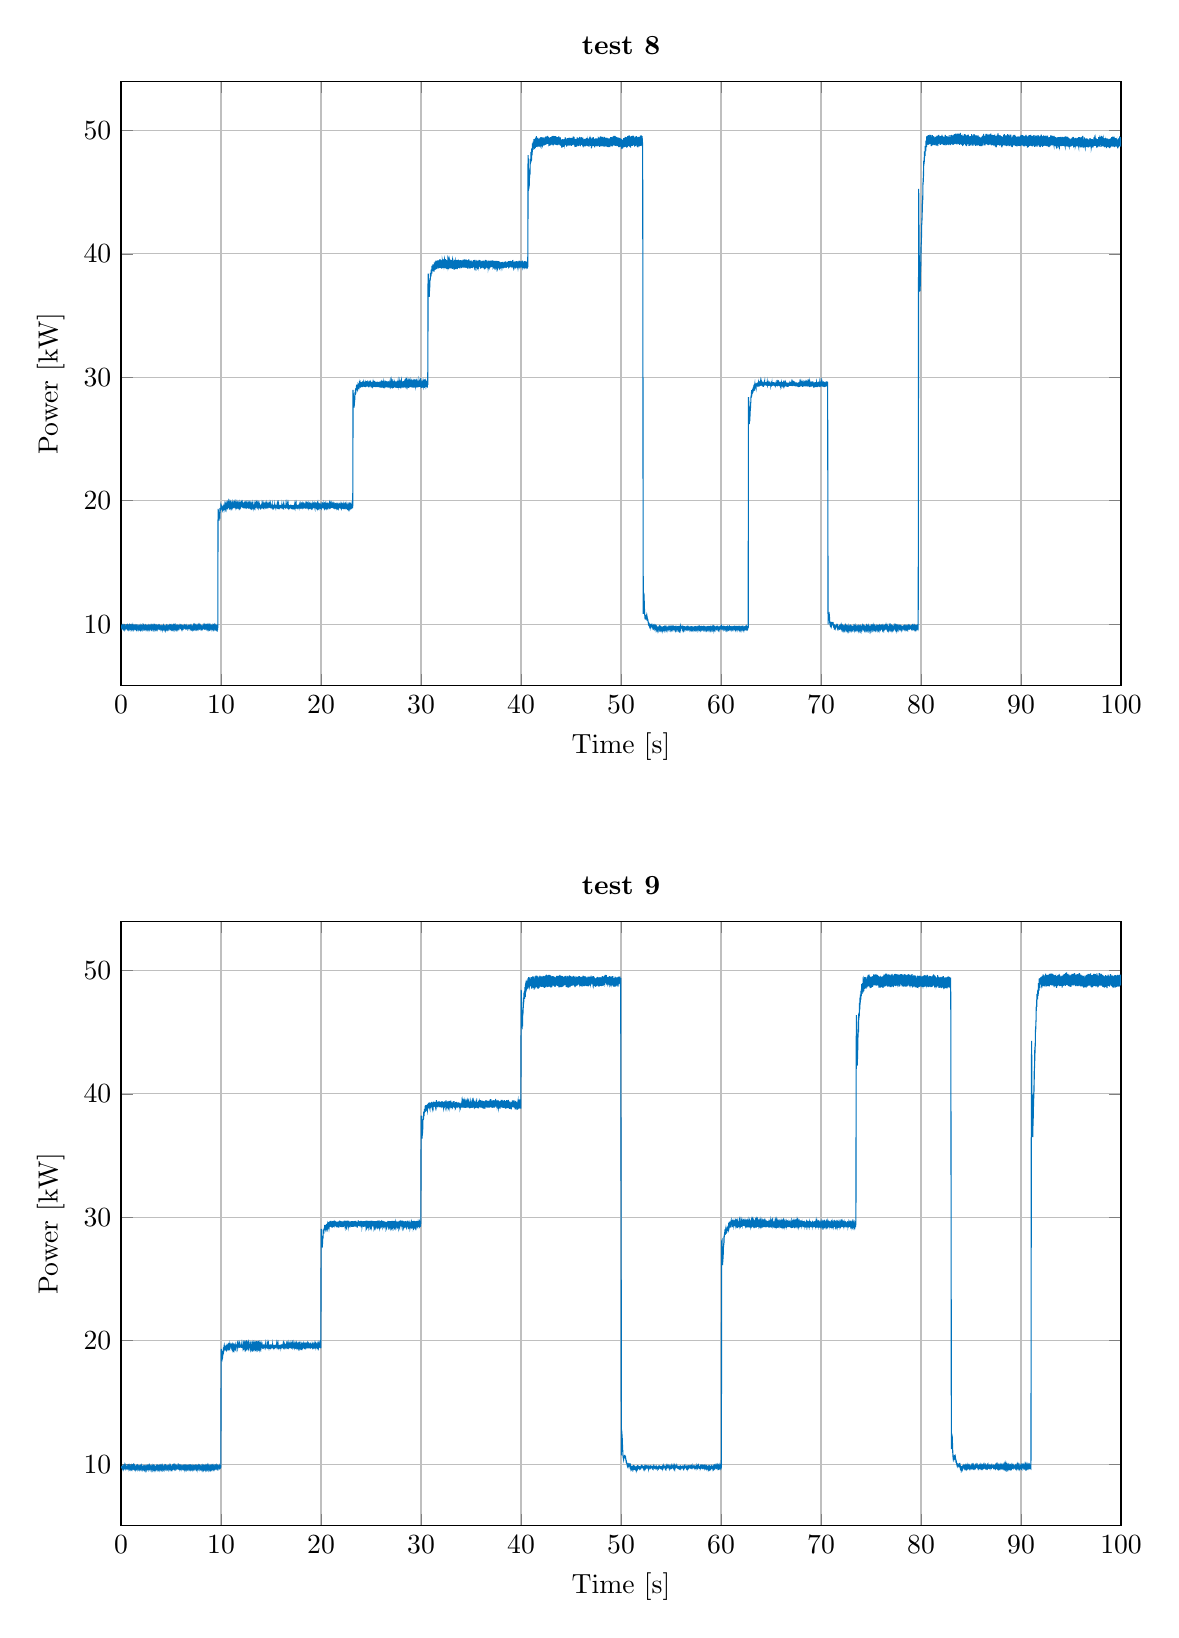
\begin{tikzpicture}

\begin{axis}[%
width=5in,
height=3.024in,
at={(1.152in,5.175in)},
scale only axis,
xmin=0,
xmax=100,
ymajorgrids,
xmajorgrids,
xlabel={Time [s]},
ymin=5,
ymax=54,
ylabel={Power [kW]},
axis background/.style={fill=white},
title style={font=\bfseries},
title={test 8}
]
\addplot [color=mycolor1,solid,forget plot]
  table[row sep=crcr]{%
0.016	9.76688251612963\\
0.032	9.80126670822115\\
0.048	9.75754409936056\\
0.064	9.70734152980283\\
0.08	9.81035307268007\\
0.096	9.77197516949088\\
0.112	9.82776676724335\\
0.128	9.77231516972259\\
0.144	9.73229128412661\\
0.16	9.82487445464699\\
0.176	9.78121176471566\\
0.192	9.82353595822829\\
0.208	9.78278890556803\\
0.224	9.72003175400604\\
0.24	9.83170083430224\\
0.256	9.80153627339916\\
0.272	9.81505225550282\\
0.288	9.78314345285466\\
0.304	9.70955782811555\\
0.32	9.83550955424742\\
0.336	9.78827835250462\\
0.352	9.81294536163614\\
0.368	9.78120880301125\\
0.384	9.71339826999873\\
0.4	9.80834016262594\\
0.416	9.77166295243651\\
0.432	9.8002435242936\\
0.448	9.76943041554963\\
0.464	9.72151443552917\\
0.48	9.79855334724726\\
0.496	9.77391001444423\\
0.512	9.8279339699553\\
0.528	9.77057714673259\\
0.544	9.72482586870899\\
0.56	9.79848660447882\\
0.576	9.78453037301712\\
0.592	9.83413532335956\\
0.608	9.78619483448377\\
0.624	9.71519771140912\\
0.64	9.81173960930456\\
0.656	9.76376725537683\\
0.672	9.82783104364907\\
0.688	9.77260383293134\\
0.704	9.70428941312654\\
0.72	9.81604776854289\\
0.736	9.79042537056004\\
0.752	9.82240878930782\\
0.768	9.79557212028888\\
0.784	9.72285870648236\\
0.8	9.81018152194638\\
0.816	9.77416705198651\\
0.832	9.84920029076297\\
0.848	9.79111508172688\\
0.864	9.72408968380842\\
0.88	9.8214510304392\\
0.896	9.77746848875694\\
0.912	9.82542675285464\\
0.928	9.75862301617776\\
0.944	9.68777655601492\\
0.96	9.7801950957921\\
0.976	9.74501803267333\\
0.992	9.82254302306233\\
1.008	9.78939277502938\\
1.024	9.71000208111662\\
1.04	9.80167259398623\\
1.056	9.7821073437088\\
1.072	9.84995152948031\\
1.088	9.79652131487928\\
1.104	9.7027657528374\\
1.12	9.79152442215694\\
1.136	9.75161468517418\\
1.152	9.8395035812992\\
1.168	9.76238919467365\\
1.184	9.70329614435497\\
1.2	9.79170983676165\\
1.216	9.75739544644562\\
1.232	9.8242151324909\\
1.248	9.76710640650664\\
1.264	9.68851332106347\\
1.28	9.78697878108676\\
1.296	9.77143910786893\\
1.312	9.82363711662156\\
1.328	9.76850704579906\\
1.344	9.71046875968203\\
1.36	9.80942769278896\\
1.376	9.78568868690533\\
1.392	9.82911585960516\\
1.408	9.76165178881501\\
1.424	9.70753066876593\\
1.44	9.79805186742755\\
1.456	9.76643406487604\\
1.472	9.81442456592497\\
1.488	9.73961660358693\\
1.504	9.68572108964297\\
1.52	9.79677130757456\\
1.536	9.78313874872454\\
1.552	9.83128169680672\\
1.568	9.78612073863349\\
1.584	9.69681212275362\\
1.6	9.81376664850239\\
1.616	9.78101755359582\\
1.632	9.82236034712568\\
1.648	9.74430483328607\\
1.664	9.69255045160363\\
1.68	9.79923139516197\\
1.696	9.78461599673483\\
1.712	9.81685240176827\\
1.728	9.75610600555322\\
1.744	9.68348686042403\\
1.76	9.81797863944677\\
1.776	9.79231457937574\\
1.792	9.81431513736696\\
1.808	9.74202853541923\\
1.824	9.69056272191575\\
1.84	9.79330969315986\\
1.856	9.77612768591282\\
1.872	9.82109292529563\\
1.888	9.77071969962261\\
1.904	9.69448526245878\\
1.92	9.80256521428901\\
1.936	9.73557657861913\\
1.952	9.80041075603538\\
1.968	9.76108450577979\\
1.984	9.68158541475999\\
2	9.77985976207856\\
2.016	9.75000760094089\\
2.032	9.82156250439172\\
2.048	9.79192905383481\\
2.064	9.71112709473945\\
2.08	9.78265965777364\\
2.096	9.71295620591759\\
2.112	9.81537983619642\\
2.128	9.7923624022294\\
2.144	9.68849873317481\\
2.16	9.76237018314975\\
2.176	9.74207358611414\\
2.192	9.85031211882443\\
2.208	9.80231862507264\\
2.224	9.71792675931678\\
2.24	9.78590051266873\\
2.256	9.7619206168263\\
2.272	9.85695343382533\\
2.288	9.80765004946975\\
2.304	9.71092975509773\\
2.32	9.78000438493982\\
2.336	9.74228805965951\\
2.352	9.82662109325454\\
2.368	9.79059247717394\\
2.384	9.70969223608576\\
2.4	9.77653861803379\\
2.416	9.74661779962059\\
2.432	9.82632855488625\\
2.448	9.77700342853195\\
2.464	9.70023333500084\\
2.48	9.78906536492014\\
2.496	9.75305200128796\\
2.512	9.82972021319082\\
2.528	9.79551372389316\\
2.544	9.69683646292411\\
2.56	9.77520602732169\\
2.576	9.7465627913762\\
2.592	9.82568826590802\\
2.608	9.7992950007759\\
2.624	9.70106894843558\\
2.64	9.76595437388665\\
2.656	9.7406119309273\\
2.672	9.81020866944342\\
2.688	9.77171851739345\\
2.704	9.67476172527606\\
2.72	9.77569241846723\\
2.736	9.74020793630512\\
2.752	9.82411375213276\\
2.768	9.77054218510168\\
2.784	9.7103193173811\\
2.8	9.80840006684069\\
2.816	9.7790545907307\\
2.832	9.82637138832808\\
2.848	9.77724473084057\\
2.864	9.70111488771154\\
2.88	9.80643308415018\\
2.896	9.77234533693603\\
2.912	9.8146079408256\\
2.928	9.76882991393454\\
2.944	9.71282515266007\\
2.96	9.82938492888433\\
2.976	9.78632563211893\\
2.992	9.80200680461029\\
3.008	9.75740984195725\\
3.024	9.68834992261044\\
3.04	9.80741541321671\\
3.056	9.75688390846573\\
3.072	9.79177253273646\\
3.088	9.74536630164004\\
3.104	9.68193342290925\\
3.12	9.78463698881434\\
3.136	9.73436360628003\\
3.152	9.78302609733207\\
3.168	9.7410932947323\\
3.184	9.6952888304763\\
3.2	9.80220848410441\\
3.216	9.75435770388276\\
3.232	9.82721503138204\\
3.248	9.76628204896475\\
3.264	9.690655540739\\
3.28	9.80605556143578\\
3.296	9.80083131850831\\
3.312	9.84526048200756\\
3.328	9.77879348136343\\
3.344	9.70008482667929\\
3.36	9.82642078239947\\
3.376	9.77738423031076\\
3.392	9.82508491650095\\
3.408	9.74327184502647\\
3.424	9.67925309527153\\
3.44	9.80146247054961\\
3.456	9.77319058303399\\
3.472	9.81205848267756\\
3.488	9.7566813911602\\
3.504	9.69548603796856\\
3.52	9.79855365917004\\
3.536	9.76036216421865\\
3.552	9.80189389522019\\
3.568	9.74251282176624\\
3.584	9.68197954569568\\
3.6	9.7969127656754\\
3.616	9.75308157128876\\
3.632	9.8064860720332\\
3.648	9.77875597695449\\
3.664	9.71327596447374\\
3.68	9.81011953248196\\
3.696	9.78048372493744\\
3.712	9.82664313896267\\
3.728	9.75265690503257\\
3.744	9.71516714697245\\
3.76	9.81651797446624\\
3.776	9.79960198647121\\
3.792	9.84106269229566\\
3.808	9.76956086467702\\
3.824	9.72510598771532\\
3.84	9.81940050473573\\
3.856	9.77725467787175\\
3.872	9.81672185499601\\
3.888	9.76122134624576\\
3.904	9.69144022612012\\
3.92	9.79896596095587\\
3.936	9.77451529228301\\
3.952	9.80232035909631\\
3.968	9.7259302217713\\
3.984	9.68511632090091\\
4	9.80052011297973\\
4.016	9.7887693543718\\
4.032	9.81929483419097\\
4.048	9.72840732593049\\
4.064	9.67560817800935\\
4.08	9.79064611123195\\
4.096	9.76212072030235\\
4.112	9.7866501904994\\
4.128	9.72426213688009\\
4.144	9.64354841727051\\
4.16	9.77193631947375\\
4.176	9.76515496575586\\
4.192	9.81145761922846\\
4.208	9.75349530728531\\
4.224	9.70132510349215\\
4.24	9.80404640043288\\
4.256	9.76941646602596\\
4.272	9.84369677136705\\
4.288	9.78347862167858\\
4.304	9.70425492671778\\
4.32	9.79998708390627\\
4.336	9.78020603272278\\
4.352	9.80982083124049\\
4.368	9.75817185077296\\
4.384	9.6887732630391\\
4.4	9.80291081987669\\
4.416	9.79095793049135\\
4.432	9.81825946268903\\
4.448	9.76828336223027\\
4.464	9.66921649558806\\
4.48	9.7925440210439\\
4.496	9.76765941687199\\
4.512	9.80439564125334\\
4.528	9.73928538394185\\
4.544	9.67848348025197\\
4.56	9.79038901883677\\
4.576	9.74079559635201\\
4.592	9.80809234668353\\
4.608	9.74881494823721\\
4.624	9.68073946086242\\
4.64	9.79603405279541\\
4.656	9.77277798888705\\
4.672	9.81499315279527\\
4.688	9.75366502794014\\
4.704	9.69127182823601\\
4.72	9.79450797528226\\
4.736	9.76231665516159\\
4.752	9.7984346605633\\
4.768	9.75363103646665\\
4.784	9.70430019834568\\
4.8	9.80615882889224\\
4.816	9.78061729243072\\
4.832	9.82827211751004\\
4.848	9.75938592778989\\
4.864	9.71245852701746\\
4.88	9.80190451859849\\
4.896	9.7469261957526\\
4.912	9.81350092422272\\
4.928	9.76629746754966\\
4.944	9.70428195043099\\
4.96	9.80222466464911\\
4.976	9.75899273608029\\
4.992	9.81127590756678\\
5.008	9.74449972089937\\
5.024	9.67908029635132\\
5.04	9.76778575885026\\
5.056	9.74320981886255\\
5.072	9.80653430798869\\
5.088	9.74653931568599\\
5.104	9.6713618318613\\
5.12	9.76669056705391\\
5.136	9.73219254851773\\
5.152	9.81804561154221\\
5.168	9.77250121672183\\
5.184	9.70037081330083\\
5.2	9.76973235178209\\
5.216	9.7797163680518\\
5.232	9.85203395482931\\
5.248	9.79392002967617\\
5.264	9.6895634223441\\
5.28	9.77691945863985\\
5.296	9.75978995922362\\
5.312	9.82518884964704\\
5.328	9.76445754447953\\
5.344	9.68090151034198\\
5.36	9.77991352907235\\
5.376	9.77638906193726\\
5.392	9.84294242645283\\
5.408	9.77479387101572\\
5.424	9.69879340917481\\
5.44	9.77328736182207\\
5.456	9.76310949074869\\
5.472	9.82570029841911\\
5.488	9.73997544192055\\
5.504	9.66755398658826\\
5.52	9.76872311569184\\
5.536	9.76043962340791\\
5.552	9.80110319792727\\
5.568	9.73669414036534\\
5.584	9.67616617620101\\
5.6	9.80123843089499\\
5.616	9.77322129153768\\
5.632	9.82091493586857\\
5.648	9.75312365516402\\
5.664	9.69289743809424\\
5.68	9.79509040127161\\
5.696	9.7604546006725\\
5.712	9.79012769481976\\
5.728	9.74657429140615\\
5.744	9.68873609629255\\
5.76	9.77971320293428\\
5.776	9.74380981457722\\
5.792	9.79840743330833\\
5.808	9.74559467559975\\
5.824	9.70713939635414\\
5.84	9.82127514890113\\
5.856	9.797146264514\\
5.872	9.84691758751472\\
5.888	9.76632469934486\\
5.904	9.74228195057239\\
5.92	9.81851866813034\\
5.936	9.77806170892652\\
5.952	9.80785323146045\\
5.968	9.7542222749021\\
5.984	9.71366565561235\\
6	9.81672946240342\\
6.016	9.76036929778663\\
6.032	9.80007410725964\\
6.048	9.75949610995725\\
6.064	9.69257884515835\\
6.08	9.78343671683136\\
6.096	9.73881307235757\\
6.112	9.78261056044925\\
6.128	9.73818195184761\\
6.144	9.67327661579843\\
6.16	9.77425623950975\\
6.176	9.74391500203547\\
6.192	9.79799470687659\\
6.208	9.74550322869018\\
6.224	9.69839848234612\\
6.24	9.77387623998187\\
6.256	9.74714991951616\\
6.272	9.78455603496245\\
6.288	9.74264569469411\\
6.304	9.7180916783729\\
6.32	9.81662014200345\\
6.336	9.77129733986349\\
6.352	9.81139736270958\\
6.368	9.7365553154118\\
6.384	9.7159671680735\\
6.4	9.80985466914098\\
6.416	9.76739658309823\\
6.432	9.79974212368258\\
6.448	9.74229997184372\\
6.464	9.70388074971741\\
6.48	9.80716185550202\\
6.496	9.77125365344607\\
6.512	9.80702066926406\\
6.528	9.74017946416627\\
6.544	9.71203169520501\\
6.56	9.82407302073712\\
6.576	9.78023292989196\\
6.592	9.78305631812564\\
6.608	9.70661211844461\\
6.624	9.66130077427859\\
6.64	9.76451793135915\\
6.656	9.74304619743482\\
6.672	9.78735974726903\\
6.688	9.70996138450967\\
6.704	9.69808051339184\\
6.72	9.79049264498001\\
6.736	9.75855559513832\\
6.752	9.79813814383427\\
6.768	9.72341940348779\\
6.784	9.67506521729586\\
6.8	9.78304274038547\\
6.816	9.77706358990241\\
6.832	9.81976145870388\\
6.848	9.76129008930748\\
6.864	9.7366096750752\\
6.88	9.83227996911402\\
6.896	9.80955428841037\\
6.912	9.84365765875086\\
6.928	9.76334213112197\\
6.944	9.70002458018841\\
6.96	9.79666133075056\\
6.976	9.74374253436015\\
6.992	9.77326182603045\\
7.008	9.73276386813553\\
7.024	9.67934195463415\\
7.04	9.77878952111631\\
7.056	9.72145570957657\\
7.072	9.77615624711614\\
7.088	9.74011990410727\\
7.104	9.67004435842929\\
7.12	9.74205069533246\\
7.136	9.71519627530518\\
7.152	9.78485625937745\\
7.168	9.75532593586363\\
7.184	9.67120591818673\\
7.2	9.75632906688399\\
7.216	9.76221155914391\\
7.232	9.84134950009938\\
7.248	9.76433942809071\\
7.264	9.6872168782831\\
7.28	9.75598058790699\\
7.296	9.76956687135316\\
7.312	9.84041996440623\\
7.328	9.77956548850719\\
7.344	9.6842782038533\\
7.36	9.74119294477434\\
7.376	9.74725441802156\\
7.392	9.84626658828865\\
7.408	9.78736156972949\\
7.424	9.70210416700046\\
7.44	9.76372071612322\\
7.456	9.74836928382424\\
7.472	9.8298511360898\\
7.488	9.77467577607693\\
7.504	9.69016292881792\\
7.52	9.75423066303624\\
7.536	9.73545501782726\\
7.552	9.8206847002786\\
7.568	9.76844273188235\\
7.584	9.68461035551239\\
7.6	9.74242997422935\\
7.616	9.71531564316562\\
7.632	9.80423265589424\\
7.648	9.7601362491047\\
7.664	9.68524992012837\\
7.68	9.74883212151302\\
7.696	9.74516208522349\\
7.712	9.84279867524755\\
7.728	9.77592100616309\\
7.744	9.69745241624789\\
7.76	9.76255443207022\\
7.776	9.75205712370546\\
7.792	9.84359694790883\\
7.808	9.79514192261784\\
7.824	9.73735497424194\\
7.84	9.78873987008067\\
7.856	9.75129896827352\\
7.872	9.84954354196145\\
7.888	9.78453466066247\\
7.904	9.71840909483098\\
7.92	9.77053135085391\\
7.936	9.74432412277822\\
7.952	9.81645881696442\\
7.968	9.75480726167704\\
7.984	9.68680430963\\
8	9.74564849429033\\
8.016	9.72963300599273\\
8.032	9.78002802461357\\
8.048	9.73105319866537\\
8.064	9.65861088804358\\
8.08	9.71475402490073\\
8.096	9.71747528468786\\
8.112	9.78754131944816\\
8.128	9.75556093572932\\
8.144	9.69542523766653\\
8.16	9.78591319391143\\
8.176	9.77902238622146\\
8.192	9.83673968170622\\
8.208	9.77506823248632\\
8.224	9.7310024551208\\
8.24	9.79916959345902\\
8.256	9.80173458158947\\
8.272	9.85852188353803\\
8.288	9.77301543239039\\
8.304	9.72996946251236\\
8.32	9.79808957105316\\
8.336	9.76646373842016\\
8.352	9.84389624851249\\
8.368	9.75801138546834\\
8.384	9.70464668570813\\
8.4	9.75798608739132\\
8.416	9.74989570919216\\
8.432	9.82280775717672\\
8.448	9.76012750598798\\
8.464	9.70812308917231\\
8.48	9.76778296063748\\
8.496	9.74239142398628\\
8.512	9.81829875988872\\
8.528	9.75211514524405\\
8.544	9.69211822604231\\
8.56	9.7715340165887\\
8.576	9.74640431083974\\
8.592	9.82413777379314\\
8.608	9.76888929477717\\
8.624	9.69355141397877\\
8.64	9.74896285710672\\
8.656	9.75258568404599\\
8.672	9.83635571353037\\
8.688	9.76404901937397\\
8.704	9.66616068900808\\
8.72	9.73638194270896\\
8.736	9.75395826825594\\
8.752	9.83395426252902\\
8.768	9.75790294481092\\
8.784	9.68619681084743\\
8.8	9.77573248945661\\
8.816	9.76776569737985\\
8.832	9.83865234408207\\
8.848	9.75097468694615\\
8.864	9.67448233275514\\
8.88	9.74661462877006\\
8.896	9.7480681717903\\
8.912	9.82112144348608\\
8.928	9.74416030298056\\
8.944	9.68682372764344\\
8.96	9.76258616784435\\
8.976	9.74274741066447\\
8.992	9.80403781434619\\
9.008	9.75351316538191\\
9.024	9.67177265010664\\
9.04	9.7430959406787\\
9.056	9.72352304307748\\
9.072	9.80129626460071\\
9.088	9.75413487450805\\
9.104	9.70784220801071\\
9.12	9.77636924164898\\
9.136	9.75930128389941\\
9.152	9.83531501407649\\
9.168	9.77544464459319\\
9.184	9.69253849943213\\
9.2	9.77396336941764\\
9.216	9.77657079740341\\
9.232	9.84036377615081\\
9.248	9.77408589037318\\
9.264	9.68898340664181\\
9.28	9.78128308805702\\
9.296	9.80009987017374\\
9.312	9.85389943521063\\
9.328	9.75297627636813\\
9.344	9.6924441162298\\
9.36	9.80042581507418\\
9.376	9.79419356937403\\
9.392	9.84911388558142\\
9.408	9.73538716911256\\
9.424	9.68425789442589\\
9.44	9.77332839586099\\
9.456	9.78468442262044\\
9.472	9.82204112920362\\
9.488	9.74708632954697\\
9.504	9.68354969802562\\
9.52	9.78186841557426\\
9.536	9.77530953850123\\
9.552	9.81073245751794\\
9.568	9.73755476282816\\
9.584	9.67108144673591\\
9.6	9.77511156508012\\
9.616	9.77898638671404\\
9.632	9.82504959924993\\
9.648	9.75260269110732\\
9.664	9.67702293244075\\
9.68	9.77519126551318\\
9.696	17.8560997486441\\
9.712	19.3317559612937\\
9.728	19.1307270208216\\
9.744	18.9409069267782\\
9.76	18.8875421407511\\
9.776	18.7431518739233\\
9.792	18.6580033244411\\
9.808	18.3880309921695\\
9.824	18.6904882202812\\
9.84	18.7552111350607\\
9.856	18.7955140106475\\
9.872	19.0129382783991\\
9.888	18.9343650319984\\
9.904	19.2210665076048\\
9.92	19.2167144913738\\
9.936	19.4156547464794\\
9.952	19.2952832794037\\
9.968	19.2975176801068\\
9.984	19.5123085054123\\
10	19.4323669564606\\
10.016	19.4672267169912\\
10.032	19.3332590014944\\
10.048	19.5231456527388\\
10.064	19.4749948692252\\
10.08	19.4606409614458\\
10.096	19.3865656131167\\
10.112	19.3338865446942\\
10.128	19.4837888446628\\
10.144	19.4718180724555\\
10.16	19.4574234805144\\
10.176	19.4898686216038\\
10.192	19.3912814881103\\
10.208	19.5304982161064\\
10.224	19.520292915643\\
10.24	19.4725882575859\\
10.256	19.4924317464003\\
10.272	19.4371649821043\\
10.288	19.5355148706309\\
10.304	19.4864288899243\\
10.32	19.4939135331753\\
10.336	19.5182580959949\\
10.352	19.4590322056096\\
10.368	19.5826072302575\\
10.384	19.4582154847345\\
10.4	19.5858643622985\\
10.416	19.5227667828497\\
10.432	19.4517002419738\\
10.448	19.6268633227837\\
10.464	19.4888295559736\\
10.48	19.6631153925414\\
10.496	19.5968587468867\\
10.512	19.4964849877434\\
10.528	19.6724098941325\\
10.544	19.5575016738631\\
10.56	19.6629322751402\\
10.576	19.5551643953683\\
10.592	19.5138548618743\\
10.608	19.6250402299791\\
10.624	19.5745755904395\\
10.64	19.681491232703\\
10.656	19.5684888503774\\
10.672	19.5122630143226\\
10.688	19.6276248844025\\
10.704	19.6130119087638\\
10.72	19.7350838075075\\
10.736	19.6007978260301\\
10.752	19.561846992996\\
10.768	19.6128060413643\\
10.784	19.573915831523\\
10.8	19.7072299021751\\
10.816	19.58911378232\\
10.832	19.5234992085348\\
10.848	19.6161510835108\\
10.864	19.551376240204\\
10.88	19.6661859252241\\
10.896	19.5269185791918\\
10.912	19.4886353326526\\
10.928	19.5865038645685\\
10.944	19.5855779971464\\
10.96	19.698898756217\\
10.976	19.5795941146611\\
10.992	19.4861067370652\\
11.008	19.5840073018299\\
11.024	19.5292688925877\\
11.04	19.6283827177278\\
11.056	19.507475499928\\
11.072	19.461910622677\\
11.088	19.5979196594629\\
11.104	19.5823815857835\\
11.12	19.6950969284291\\
11.136	19.5586570784222\\
11.152	19.5201750954123\\
11.168	19.6434464050416\\
11.184	19.583192879939\\
11.2	19.6747972052404\\
11.216	19.5357851371188\\
11.232	19.5167691679337\\
11.248	19.6142828594775\\
11.264	19.6037949665122\\
11.28	19.6713079437157\\
11.296	19.5200100783074\\
11.312	19.5106695966919\\
11.328	19.6032265095905\\
11.344	19.5656769226009\\
11.36	19.6776852831439\\
11.376	19.5289110140086\\
11.392	19.5111452030148\\
11.408	19.6221473093952\\
11.424	19.6129697425636\\
11.44	19.711909239006\\
11.456	19.5532015819063\\
11.472	19.4822177885451\\
11.488	19.5787550250619\\
11.504	19.5553175497245\\
11.52	19.6739093631977\\
11.536	19.5511498936116\\
11.552	19.5080224374094\\
11.568	19.5973231153856\\
11.584	19.5600795025129\\
11.6	19.6525601985617\\
11.616	19.5524923998165\\
11.632	19.5226895699395\\
11.648	19.639260245484\\
11.664	19.5825400379335\\
11.68	19.6802942073984\\
11.696	19.5318485951422\\
11.712	19.4993715106933\\
11.728	19.6069631893714\\
11.744	19.5537921300152\\
11.76	19.6405243739622\\
11.776	19.5288528771684\\
11.792	19.4669409608843\\
11.808	19.5937955271306\\
11.824	19.5711907487375\\
11.84	19.6754483297699\\
11.856	19.5289863641404\\
11.872	19.4862689051193\\
11.888	19.6062050234846\\
11.904	19.587885466394\\
11.92	19.6589015502865\\
11.936	19.5010336138662\\
11.952	19.4744080898206\\
11.968	19.6043225051702\\
11.984	19.5910853919544\\
12	19.672382408826\\
12.016	19.5200487760239\\
12.032	19.5205630258831\\
12.048	19.6223714241767\\
12.064	19.611413995818\\
12.08	19.6992905490012\\
12.096	19.5468508580322\\
12.112	19.5308026163444\\
12.128	19.6273050339974\\
12.144	19.5892211167947\\
12.16	19.6748762350713\\
12.176	19.5060983628349\\
12.192	19.5041347039843\\
12.208	19.6008771335158\\
12.224	19.55848684593\\
12.24	19.6209926051874\\
12.256	19.4852256355425\\
12.272	19.4937433099324\\
12.288	19.6064941867014\\
12.304	19.572975231874\\
12.32	19.656281728281\\
12.336	19.5078378620517\\
12.352	19.5380050598309\\
12.368	19.6419075107899\\
12.384	19.5989431206645\\
12.4	19.6750907225319\\
12.416	19.5368091940055\\
12.432	19.5386014376538\\
12.448	19.6459784394303\\
12.464	19.5785197039265\\
12.48	19.6598308847315\\
12.496	19.5078728401608\\
12.512	19.4758065406186\\
12.528	19.5752925472198\\
12.544	19.5480927060288\\
12.56	19.6386938257075\\
12.576	19.5004487893156\\
12.592	19.4903830374599\\
12.608	19.6116946241194\\
12.624	19.5720961587077\\
12.64	19.6654818363827\\
12.656	19.5371030450688\\
12.672	19.5151788101613\\
12.688	19.5926319230257\\
12.704	19.5544333140548\\
12.72	19.6513397496621\\
12.736	19.5156351045116\\
12.752	19.4923562362176\\
12.768	19.6294256128449\\
12.784	19.6386774675081\\
12.8	19.7092439181343\\
12.816	19.5662680609522\\
12.832	19.5195954010938\\
12.848	19.5801607648747\\
12.864	19.5475393976938\\
12.88	19.6359911887\\
12.896	19.5149523729434\\
12.912	19.4740082179797\\
12.928	19.5932285859381\\
12.944	19.5618940391613\\
12.96	19.6454075288095\\
12.976	19.5124456128073\\
12.992	19.4730629826039\\
13.008	19.5863715166506\\
13.024	19.5426738296929\\
13.04	19.624951295834\\
13.056	19.5043189979892\\
13.072	19.4500709195317\\
13.088	19.5598227612299\\
13.104	19.5646176010872\\
13.12	19.6720954862148\\
13.136	19.5384045313751\\
13.152	19.4990986045345\\
13.168	19.5964140280584\\
13.184	19.5791962158861\\
13.2	19.6566785219443\\
13.216	19.531189010192\\
13.232	19.4607916294034\\
13.248	19.5853520105484\\
13.264	19.5514870793847\\
13.28	19.6761621481474\\
13.296	19.5119529004054\\
13.312	19.468899731698\\
13.328	19.5906246208865\\
13.344	19.6041776483315\\
13.36	19.6824758310643\\
13.376	19.5160360939668\\
13.392	19.4589681964386\\
13.408	19.5786670004494\\
13.424	19.5690402292059\\
13.44	19.6627080953876\\
13.456	19.4989469086582\\
13.472	19.4848818747218\\
13.488	19.5628875216242\\
13.504	19.6120985299705\\
13.52	19.6972662226957\\
13.536	19.5192240913212\\
13.552	19.5136958099265\\
13.568	19.6124508964528\\
13.584	19.561117203315\\
13.6	19.6557562459571\\
13.616	19.4905705271867\\
13.632	19.473130551684\\
13.648	19.5874916106852\\
13.664	19.5852424057335\\
13.68	19.6605584225488\\
13.696	19.4958239449974\\
13.712	19.4452827818446\\
13.728	19.5671716341752\\
13.744	19.543107471729\\
13.76	19.6288144730102\\
13.776	19.4924967961416\\
13.792	19.4748402825493\\
13.808	19.5748644348764\\
13.824	19.559908769748\\
13.84	19.6418491984805\\
13.856	19.5072430892063\\
13.872	19.4849058242673\\
13.888	19.5805883440512\\
13.904	19.5365486176239\\
13.92	19.6609615481818\\
13.936	19.5245564961773\\
13.952	19.4787163753994\\
13.968	19.5755036527465\\
13.984	19.5579133480232\\
14	19.6727757537855\\
14.016	19.519050649704\\
14.032	19.488407468797\\
14.048	19.6080661509109\\
14.064	19.590394077618\\
14.08	19.6833247322471\\
14.096	19.531510452274\\
14.112	19.5029142513868\\
14.128	19.5961720420617\\
14.144	19.5688507497196\\
14.16	19.651118566181\\
14.176	19.5120822867722\\
14.192	19.4862725676921\\
14.208	19.5876772824666\\
14.224	19.5515612506378\\
14.24	19.6441706961489\\
14.256	19.4915293531808\\
14.272	19.4564398407227\\
14.288	19.5766848356784\\
14.304	19.5559648676418\\
14.32	19.6205070777992\\
14.336	19.5184541759484\\
14.352	19.4993838469862\\
14.368	19.5906173999031\\
14.384	19.5400467675075\\
14.4	19.6358527968791\\
14.416	19.5223937376867\\
14.432	19.498294721895\\
14.448	19.5880281096334\\
14.464	19.5515341301811\\
14.48	19.6322974209872\\
14.496	19.5046894679693\\
14.512	19.481655721186\\
14.528	19.5758905897904\\
14.544	19.548647878004\\
14.56	19.6467508790424\\
14.576	19.4782338027442\\
14.592	19.4719305702637\\
14.608	19.5699346587275\\
14.624	19.5580657212684\\
14.64	19.6283099548544\\
14.656	19.4775553078864\\
14.672	19.4547080811013\\
14.688	19.5546157270249\\
14.704	19.5369782531269\\
14.72	19.6159006107127\\
14.736	19.4751412332119\\
14.752	19.4854274002926\\
14.768	19.602611646761\\
14.784	19.5894531247944\\
14.8	19.6384550021822\\
14.816	19.509480221073\\
14.832	19.4993492245234\\
14.848	19.6022379518609\\
14.864	19.5834353961422\\
14.88	19.6818718968413\\
14.896	19.5185776136251\\
14.912	19.4960400458506\\
14.928	19.5734568081457\\
14.944	19.5478861470968\\
14.96	19.6347140029187\\
14.976	19.4857538645777\\
14.992	19.4702494015433\\
15.008	19.5622246570293\\
15.024	19.5334525962067\\
15.04	19.6808101850009\\
15.056	19.5154382291845\\
15.072	19.50020530156\\
15.088	19.5785307064857\\
15.104	19.5710321245109\\
15.12	19.6642030792386\\
15.136	19.4875606771992\\
15.152	19.4428331960114\\
15.168	19.5187019420891\\
15.184	19.5156296334776\\
15.2	19.6254244198166\\
15.216	19.4484628252316\\
15.232	19.418831202899\\
15.248	19.5307871184043\\
15.264	19.546466825207\\
15.28	19.6743005801131\\
15.296	19.4864042461646\\
15.312	19.4711810969641\\
15.328	19.5653353826864\\
15.344	19.5701213476621\\
15.36	19.6602834328498\\
15.376	19.482691232016\\
15.392	19.4721343290953\\
15.408	19.5520537124773\\
15.424	19.558140337063\\
15.44	19.691012316124\\
15.456	19.4825902106126\\
15.472	19.4303631337399\\
15.488	19.5424638817892\\
15.504	19.5339217068344\\
15.52	19.6531556330811\\
15.536	19.4565517896621\\
15.552	19.4480399440251\\
15.568	19.5346201173981\\
15.584	19.5482929810556\\
15.6	19.6335571718879\\
15.616	19.460816477236\\
15.632	19.4395309034935\\
15.648	19.5488288000156\\
15.664	19.5420275958798\\
15.68	19.6341750007665\\
15.696	19.4698866196253\\
15.712	19.4460113477953\\
15.728	19.5553866092216\\
15.744	19.5718174280794\\
15.76	19.6587916240787\\
15.776	19.4984795471067\\
15.792	19.4623312587082\\
15.808	19.5682917811016\\
15.824	19.5492414076569\\
15.84	19.6611530234308\\
15.856	19.48610035612\\
15.872	19.4632047289923\\
15.888	19.5595191327298\\
15.904	19.5502169945856\\
15.92	19.6578305164654\\
15.936	19.481989857318\\
15.952	19.4716666750204\\
15.968	19.5518841166836\\
15.984	19.5434158768066\\
16	19.6717717135769\\
16.016	19.4929434549386\\
16.032	19.4712217642828\\
16.048	19.5684731931761\\
16.064	19.5734145045483\\
16.08	19.6772983274082\\
16.096	19.5277862713285\\
16.112	19.4959865638916\\
16.128	19.5834170826514\\
16.144	19.5846574110183\\
16.16	19.6960954439298\\
16.176	19.4880914761207\\
16.192	19.4491158145389\\
16.208	19.537779445166\\
16.224	19.562544476193\\
16.24	19.6480929599977\\
16.256	19.4615280451448\\
16.272	19.4330847038225\\
16.288	19.551616315607\\
16.304	19.5387945871763\\
16.32	19.6584506997202\\
16.336	19.4840258294573\\
16.352	19.4846314998896\\
16.368	19.5760467663056\\
16.384	19.5728475487713\\
16.4	19.6597423867315\\
16.416	19.4616085661511\\
16.432	19.4488717160099\\
16.448	19.5576640804058\\
16.464	19.5432403587039\\
16.48	19.6439668029809\\
16.496	19.4291165895437\\
16.512	19.4426695467173\\
16.528	19.5789206805508\\
16.544	19.5984762781472\\
16.56	19.6919653404311\\
16.576	19.5127616492533\\
16.592	19.4921101643266\\
16.608	19.5859045521868\\
16.624	19.5899300549006\\
16.64	19.6796765403637\\
16.656	19.4753669849318\\
16.672	19.4547057665381\\
16.688	19.5544250940342\\
16.704	19.5483089919141\\
16.72	19.6522302294964\\
16.736	19.4892205495694\\
16.752	19.4474953766536\\
16.768	19.5510352075772\\
16.784	19.4982099442659\\
16.8	19.6327790822239\\
16.816	19.4596141133744\\
16.832	19.4397045720277\\
16.848	19.5241291385489\\
16.864	19.5049996838157\\
16.88	19.6485316076398\\
16.896	19.4891940278241\\
16.912	19.4726220034083\\
16.928	19.5606577689492\\
16.944	19.5435741639413\\
16.96	19.6788974047797\\
16.976	19.506326977516\\
16.992	19.4834332287929\\
17.008	19.5673599640364\\
17.024	19.5493971287919\\
17.04	19.6507284410949\\
17.056	19.4733946507159\\
17.072	19.4430376073537\\
17.088	19.5392499795136\\
17.104	19.5163900944432\\
17.12	19.6363497100307\\
17.136	19.4420605521202\\
17.152	19.4197147853296\\
17.168	19.5338197331131\\
17.184	19.541760927746\\
17.2	19.6480325547452\\
17.216	19.4432228366682\\
17.232	19.4177226546512\\
17.248	19.5589287875212\\
17.264	19.554555315252\\
17.28	19.6627451212798\\
17.296	19.4620992423539\\
17.312	19.4373461372115\\
17.328	19.5981363749286\\
17.344	19.5972953026494\\
17.36	19.6727910121237\\
17.376	19.4677826356176\\
17.392	19.4117468137087\\
17.408	19.5465135823328\\
17.424	19.5345550717387\\
17.44	19.6292170897189\\
17.456	19.4401969492418\\
17.472	19.4285586187896\\
17.488	19.5896816425881\\
17.504	19.5905788415306\\
17.52	19.6742549869105\\
17.536	19.4685176107769\\
17.552	19.4541769144032\\
17.568	19.5915525024144\\
17.584	19.5608624473552\\
17.6	19.6546208410602\\
17.616	19.4411720297858\\
17.632	19.423349074808\\
17.648	19.5702467401925\\
17.664	19.5540718378542\\
17.68	19.6494619809121\\
17.696	19.4171940162001\\
17.712	19.4221096371347\\
17.728	19.5805005430432\\
17.744	19.6013461788467\\
17.76	19.6915343386432\\
17.776	19.4597745088527\\
17.792	19.4223141675345\\
17.808	19.5896554747374\\
17.824	19.5779307063423\\
17.84	19.6322741830941\\
17.856	19.4306835874427\\
17.872	19.4228306272526\\
17.888	19.6324604094733\\
17.904	19.6082366097888\\
17.92	19.6673656305616\\
17.936	19.4857629321996\\
17.952	19.4652133186003\\
17.968	19.6440771536201\\
17.984	19.6004160673624\\
18	19.6432937570118\\
18.016	19.4528992543355\\
18.032	19.4556940678986\\
18.048	19.6367587672507\\
18.064	19.5897544162763\\
18.08	19.6419347267954\\
18.096	19.4425251115125\\
18.112	19.4520841680347\\
18.128	19.6167624521379\\
18.144	19.5607955408082\\
18.16	19.6260174071373\\
18.176	19.4069305272216\\
18.192	19.4224351943523\\
18.208	19.6227451590131\\
18.224	19.5767870866212\\
18.24	19.6277915628889\\
18.256	19.4125315760427\\
18.272	19.4150106636086\\
18.288	19.605800843366\\
18.304	19.5695193162469\\
18.32	19.6119086456511\\
18.336	19.4249499311369\\
18.352	19.4233824260443\\
18.368	19.6198645421091\\
18.384	19.5995128802492\\
18.4	19.658407757832\\
18.416	19.4523590868446\\
18.432	19.4400986860985\\
18.448	19.6157986420487\\
18.464	19.5798795282131\\
18.48	19.6321672441278\\
18.496	19.4601875230618\\
18.512	19.4467580330739\\
18.528	19.6322913530076\\
18.544	19.5661990835522\\
18.56	19.6354653965978\\
18.576	19.4797462921646\\
18.592	19.4688494144013\\
18.608	19.6141177971529\\
18.624	19.5489355512325\\
18.64	19.6232768136876\\
18.656	19.4543972042696\\
18.672	19.4421860702344\\
18.688	19.5847591493319\\
18.704	19.5406152760105\\
18.72	19.6250590197105\\
18.736	19.4435203177556\\
18.752	19.4047146739066\\
18.768	19.5329855472509\\
18.784	19.510665564001\\
18.8	19.5781078902379\\
18.816	19.4414995508044\\
18.832	19.4260571333117\\
18.848	19.6110888950271\\
18.864	19.583302321546\\
18.88	19.6480986506497\\
18.896	19.4972518216664\\
18.912	19.4721527160252\\
18.928	19.6216310741394\\
18.944	19.5609674382707\\
18.96	19.6065709558143\\
18.976	19.4621511991191\\
18.992	19.4295414290635\\
19.008	19.5782489688939\\
19.024	19.5325369750955\\
19.04	19.5912664969863\\
19.056	19.4625916935951\\
19.072	19.4316983011858\\
19.088	19.5803919968637\\
19.104	19.5502319416978\\
19.12	19.6447765670825\\
19.136	19.5093557796971\\
19.152	19.475698158319\\
19.168	19.6371300223433\\
19.184	19.5829863344606\\
19.2	19.6339661886413\\
19.216	19.4486274060438\\
19.232	19.4482343197725\\
19.248	19.6065416845847\\
19.264	19.5743906435587\\
19.28	19.6379348470856\\
19.296	19.4728763021347\\
19.312	19.4750042844557\\
19.328	19.6265055396142\\
19.344	19.6092321580651\\
19.36	19.6654465355462\\
19.376	19.4667954443762\\
19.392	19.407037561367\\
19.408	19.5922208392443\\
19.424	19.5723075269128\\
19.44	19.6296591166391\\
19.456	19.4778499322882\\
19.472	19.4599707476182\\
19.488	19.6213909530008\\
19.504	19.6174265182007\\
19.52	19.658856812839\\
19.536	19.4752036435493\\
19.552	19.4417509052717\\
19.568	19.6244049832556\\
19.584	19.5896643312036\\
19.6	19.6497059523624\\
19.616	19.4636790920773\\
19.632	19.4150949363182\\
19.648	19.5933679996792\\
19.664	19.5676900265511\\
19.68	19.6608200466611\\
19.696	19.4726240212225\\
19.712	19.4396591728644\\
19.728	19.6021381616351\\
19.744	19.5808470621479\\
19.76	19.6352592825034\\
19.776	19.4511033222695\\
19.792	19.4171266743624\\
19.808	19.6042192638725\\
19.824	19.5720541263318\\
19.84	19.5981879545034\\
19.856	19.4180826775867\\
19.872	19.4106476402165\\
19.888	19.6107039483278\\
19.904	19.57453002234\\
19.92	19.6149362637561\\
19.936	19.4516294936352\\
19.952	19.4358433080802\\
19.968	19.617484164026\\
19.984	19.5713952567739\\
20	19.6160953990141\\
20.016	19.4536345104013\\
20.032	19.4210570054218\\
20.048	19.6053750484413\\
20.064	19.5792030887232\\
20.08	19.6096022316682\\
20.096	19.431954379602\\
20.112	19.449389770585\\
20.128	19.6670925880246\\
20.144	19.6245372838026\\
20.16	19.6368995966808\\
20.176	19.4726762737455\\
20.192	19.4647093831468\\
20.208	19.6741921336252\\
20.224	19.6379877861359\\
20.24	19.6320189114516\\
20.256	19.4646016405484\\
20.272	19.4405727556992\\
20.288	19.6483383089807\\
20.304	19.5619779848623\\
20.32	19.6135015043946\\
20.336	19.4316463566703\\
20.352	19.3948349741692\\
20.368	19.5631435239702\\
20.384	19.5448686752028\\
20.4	19.6146338647967\\
20.416	19.4184440509155\\
20.432	19.404258234404\\
20.448	19.5955017036964\\
20.464	19.597937484597\\
20.48	19.6563364891802\\
20.496	19.4617830760564\\
20.512	19.4282376094884\\
20.528	19.6146090254822\\
20.544	19.5944957598248\\
20.56	19.6308395902516\\
20.576	19.4485936448392\\
20.592	19.4263275065091\\
20.608	19.619080099836\\
20.624	19.5803091743845\\
20.64	19.6286651291017\\
20.656	19.4804447396877\\
20.672	19.4486171351122\\
20.688	19.6515626622447\\
20.704	19.6020603336137\\
20.72	19.6338981809254\\
20.736	19.4770948666223\\
20.752	19.4651431002749\\
20.768	19.6680719542739\\
20.784	19.630386595458\\
20.8	19.6523544477341\\
20.816	19.5115406689524\\
20.832	19.4836039684853\\
20.848	19.6920502754955\\
20.864	19.6185045775877\\
20.88	19.6060097326467\\
20.896	19.4846792249029\\
20.912	19.470559972091\\
20.928	19.6784387964593\\
20.944	19.6246772477603\\
20.96	19.5863520934537\\
20.976	19.454162291094\\
20.992	19.472479286641\\
21.008	19.6869627225995\\
21.024	19.624574146095\\
21.04	19.5991353635354\\
21.056	19.4816682134469\\
21.072	19.4778387922413\\
21.088	19.6679290978751\\
21.104	19.5958697667718\\
21.12	19.5840860654181\\
21.136	19.4601007987699\\
21.152	19.46401129344\\
21.168	19.6439307688765\\
21.184	19.5879837105829\\
21.2	19.5821099888266\\
21.216	19.4552828625777\\
21.232	19.4434233598525\\
21.248	19.6421132910989\\
21.264	19.5848953364313\\
21.28	19.5943458101279\\
21.296	19.4853227365401\\
21.312	19.4585815260469\\
21.328	19.643185050621\\
21.344	19.6056328844718\\
21.36	19.616167794337\\
21.376	19.4586228630096\\
21.392	19.4398383438246\\
21.408	19.6463212006192\\
21.424	19.6067862407205\\
21.44	19.6056367192861\\
21.456	19.4450467479706\\
21.472	19.4321730802574\\
21.488	19.6403554109918\\
21.504	19.6058823124757\\
21.52	19.5947400143637\\
21.536	19.4509336837198\\
21.552	19.4163294302888\\
21.568	19.6598485838867\\
21.584	19.6238452506577\\
21.6	19.5944462466909\\
21.616	19.4363888316667\\
21.632	19.4314931893633\\
21.648	19.6668367843339\\
21.664	19.631789568091\\
21.68	19.5775236207163\\
21.696	19.4021206523474\\
21.712	19.4290497829178\\
21.728	19.597201534314\\
21.744	19.5618636439849\\
21.76	19.5579230184323\\
21.776	19.413466771714\\
21.792	19.454490997284\\
21.808	19.63933758136\\
21.824	19.6057088488138\\
21.84	19.6112370620763\\
21.856	19.4773868053213\\
21.872	19.4684945108578\\
21.888	19.6518409337467\\
21.904	19.6135066359927\\
21.92	19.6214457532101\\
21.936	19.4888594771678\\
21.952	19.4628801738617\\
21.968	19.6579307979669\\
21.984	19.603544510224\\
22	19.607478116558\\
22.016	19.4709832616674\\
22.032	19.4265757321094\\
22.048	19.6110948218962\\
22.064	19.5509966602567\\
22.08	19.5597700732948\\
22.096	19.4226833588308\\
22.112	19.4139165321416\\
22.128	19.6267452579725\\
22.144	19.5887694151755\\
22.16	19.5737302829306\\
22.176	19.417432846685\\
22.192	19.4032143242165\\
22.208	19.6099395389783\\
22.224	19.5702013368647\\
22.24	19.564989125311\\
22.256	19.4428732156054\\
22.272	19.4245787035737\\
22.288	19.6536016263125\\
22.304	19.5945565495118\\
22.32	19.5615770073079\\
22.336	19.4387193607347\\
22.352	19.4326571591067\\
22.368	19.6475124077131\\
22.384	19.6054184167013\\
22.4	19.6001397533848\\
22.416	19.4554347501795\\
22.432	19.4832569786434\\
22.448	19.6660116041161\\
22.464	19.6227631718251\\
22.48	19.5859698731364\\
22.496	19.4279589880713\\
22.512	19.4515492520911\\
22.528	19.6394429924068\\
22.544	19.5675089461646\\
22.56	19.5306952813493\\
22.576	19.3981498223191\\
22.592	19.4127893046124\\
22.608	19.5789718300862\\
22.624	19.5504476608097\\
22.64	19.5406095756423\\
22.656	19.4209330232577\\
22.672	19.465173108231\\
22.688	19.6241763237433\\
22.704	19.5747529868425\\
22.72	19.5464159686985\\
22.736	19.4072282234558\\
22.752	19.4674948558793\\
22.768	19.6276928971113\\
22.784	19.5793013975323\\
22.8	19.5716863540524\\
22.816	19.4267792785959\\
22.832	19.4743279342126\\
22.848	19.6226520097678\\
22.864	19.5643646655368\\
22.88	19.5905356011738\\
22.896	19.4181676702095\\
22.912	19.4723024770242\\
22.928	19.6166807938514\\
22.944	19.5586499703198\\
22.96	19.5632114127112\\
22.976	19.4480058637613\\
22.992	19.4778439457058\\
23.008	19.6264618004139\\
23.024	19.5879129191768\\
23.04	19.5799448168693\\
23.056	19.4603349714707\\
23.072	19.4875726738282\\
23.088	19.6225686243623\\
23.104	19.5513562891487\\
23.12	19.5466569544383\\
23.136	19.436101107066\\
23.152	19.4431076049509\\
23.168	19.5784412715981\\
23.184	21.3271738170601\\
23.2	28.9761812280174\\
23.216	28.7034278635087\\
23.232	28.5879460551656\\
23.248	28.4689722606493\\
23.264	27.9422153243289\\
23.28	27.74196239121\\
23.296	27.5475518431057\\
23.312	27.8094526619361\\
23.328	27.700451078608\\
23.344	28.0021873474322\\
23.36	28.1808232239084\\
23.376	28.2051026394195\\
23.392	28.7277446770833\\
23.408	28.7452680232531\\
23.424	28.7755464588241\\
23.44	28.5881047495842\\
23.456	29.1021845964438\\
23.472	28.9497847837278\\
23.488	28.9135475878345\\
23.504	29.0930110020825\\
23.52	28.9534582222064\\
23.536	29.3074396419981\\
23.552	29.0977608738619\\
23.568	29.4035225066672\\
23.584	29.2497786733592\\
23.6	29.0681985504099\\
23.616	29.3735896485135\\
23.632	29.2599496412232\\
23.648	29.3611252693687\\
23.664	29.0924857432147\\
23.68	29.1502677533941\\
23.696	29.340864523982\\
23.712	29.2872040180088\\
23.728	29.3931148406819\\
23.744	29.0691069343713\\
23.76	29.156643460951\\
23.776	29.4811143805685\\
23.792	29.37827020368\\
23.808	29.4571453035838\\
23.824	29.2101074478716\\
23.84	29.2572389570849\\
23.856	29.6100636459803\\
23.872	29.4481465300031\\
23.888	29.4958172091512\\
23.904	29.2663091073369\\
23.92	29.2493906245267\\
23.936	29.5971101065909\\
23.952	29.3857721142585\\
23.968	29.4215450533514\\
23.984	29.2086116270507\\
24	29.328170239195\\
24.016	29.627315872157\\
24.032	29.4640791462457\\
24.048	29.4519030432502\\
24.064	29.2013285919211\\
24.08	29.3597309312137\\
24.096	29.6173736433362\\
24.112	29.4283947035307\\
24.128	29.4549720998017\\
24.144	29.2098043042457\\
24.16	29.4610402018116\\
24.176	29.6626361915609\\
24.192	29.5046951199298\\
24.208	29.5605709195911\\
24.224	29.3253326991344\\
24.24	29.5257523517466\\
24.256	29.6634959849433\\
24.272	29.4559710076124\\
24.288	29.494564036522\\
24.304	29.2548280353941\\
24.32	29.4725092890054\\
24.336	29.606714253325\\
24.352	29.4302103710441\\
24.368	29.4618787105569\\
24.384	29.2312031997243\\
24.4	29.4537569858665\\
24.416	29.6162033258584\\
24.432	29.4405651754057\\
24.448	29.4944422738692\\
24.464	29.2268600760824\\
24.48	29.4790852412078\\
24.496	29.6472091335788\\
24.512	29.4587329742119\\
24.528	29.4726123541534\\
24.544	29.2441559635418\\
24.56	29.4897672421324\\
24.576	29.6911878997582\\
24.592	29.4935302483806\\
24.608	29.5332937429689\\
24.624	29.2722242436429\\
24.64	29.5067204631821\\
24.656	29.666511031211\\
24.672	29.4842861894421\\
24.688	29.4975155179796\\
24.704	29.2584262901394\\
24.72	29.4676441596279\\
24.736	29.6587750065477\\
24.752	29.4584550046005\\
24.768	29.5036152189178\\
24.784	29.1947652175148\\
24.8	29.428026963411\\
24.816	29.6013256429514\\
24.832	29.4378624674673\\
24.848	29.4801727953723\\
24.864	29.2416533362681\\
24.88	29.4949158551085\\
24.896	29.6789031651815\\
24.912	29.5178929519904\\
24.928	29.5604351846232\\
24.944	29.3049745763599\\
24.96	29.5042702596805\\
24.976	29.6446709765497\\
24.992	29.4223884693646\\
25.008	29.4308900176188\\
25.024	29.1860016621515\\
25.04	29.4043502792146\\
25.056	29.6018221733937\\
25.072	29.4095182670484\\
25.088	29.4420319579254\\
25.104	29.1619034743373\\
25.12	29.4625624513762\\
25.136	29.6184955178272\\
25.152	29.4228758258205\\
25.168	29.4935733607827\\
25.184	29.2179489328206\\
25.2	29.5186517832885\\
25.216	29.6909937310951\\
25.232	29.4473942682431\\
25.248	29.4970538544955\\
25.264	29.2197965720642\\
25.28	29.5459606533496\\
25.296	29.7167185506597\\
25.312	29.4809526450029\\
25.328	29.5120695809606\\
25.344	29.2279516220808\\
25.36	29.4835329359249\\
25.376	29.6220914503873\\
25.392	29.4083491577685\\
25.408	29.4364700160061\\
25.424	29.2123311446766\\
25.44	29.5053017363494\\
25.456	29.6473902083525\\
25.472	29.438684909583\\
25.488	29.4557866316733\\
25.504	29.2365893752164\\
25.52	29.4586283698051\\
25.536	29.6341707106287\\
25.552	29.4112903359052\\
25.568	29.4413071320589\\
25.584	29.2160853816861\\
25.6	29.4437381899055\\
25.616	29.6202240311145\\
25.632	29.4233813010915\\
25.648	29.4589386312163\\
25.664	29.2358769963237\\
25.68	29.4170349965684\\
25.696	29.6351437727817\\
25.712	29.4363726490517\\
25.728	29.4487122658258\\
25.744	29.2045315018038\\
25.76	29.3925937362083\\
25.776	29.6269527150606\\
25.792	29.4351994154038\\
25.808	29.4099515408106\\
25.824	29.2082340811629\\
25.84	29.429257745232\\
25.856	29.6562041485452\\
25.872	29.4375501268908\\
25.888	29.4265211599121\\
25.904	29.160277766916\\
25.92	29.4268760886205\\
25.936	29.6580826113337\\
25.952	29.4833835071099\\
25.968	29.5243262439104\\
25.984	29.2402322122282\\
26	29.5267034595137\\
26.016	29.6902988641544\\
26.032	29.4586583391152\\
26.048	29.5116105950572\\
26.064	29.1754681992333\\
26.08	29.5352103304659\\
26.096	29.6531798938637\\
26.112	29.4368990340049\\
26.128	29.4884216026876\\
26.144	29.2029201552661\\
26.16	29.5677130276873\\
26.176	29.685208646606\\
26.192	29.4346585160104\\
26.208	29.4742646874202\\
26.224	29.1499230311345\\
26.24	29.541989420329\\
26.256	29.6094604266519\\
26.272	29.4036753631393\\
26.288	29.4338521715679\\
26.304	29.114232676981\\
26.32	29.4858773593082\\
26.336	29.6507320424194\\
26.352	29.4261091535841\\
26.368	29.4620532987719\\
26.384	29.1656103425163\\
26.4	29.5554702742668\\
26.416	29.7231164821786\\
26.432	29.4910241267143\\
26.448	29.4718740916746\\
26.464	29.1954965856704\\
26.48	29.4943150231371\\
26.496	29.6947492847567\\
26.512	29.4639453750199\\
26.528	29.4683335643679\\
26.544	29.2006511687785\\
26.56	29.501978541615\\
26.576	29.666555594122\\
26.592	29.4390641824899\\
26.608	29.4592079395061\\
26.624	29.1860826298154\\
26.64	29.5072285564055\\
26.656	29.6774865752895\\
26.672	29.4332245457345\\
26.688	29.4724307111036\\
26.704	29.1729064212038\\
26.72	29.5464742553925\\
26.736	29.659937177996\\
26.752	29.4204215902019\\
26.768	29.460093585823\\
26.784	29.1773134984552\\
26.8	29.5049297446532\\
26.816	29.610692973042\\
26.832	29.3923987250113\\
26.848	29.4851589977078\\
26.864	29.1718858659192\\
26.88	29.5538446605208\\
26.896	29.6277372621368\\
26.912	29.4175289291243\\
26.928	29.490939478243\\
26.944	29.1652869612265\\
26.96	29.5484484276675\\
26.976	29.6550801948032\\
26.992	29.4262082431191\\
27.008	29.5016432897874\\
27.024	29.1728005739131\\
27.04	29.5380746661095\\
27.056	29.6307929126049\\
27.072	29.4359804099415\\
27.088	29.4962065044839\\
27.104	29.1512771792832\\
27.12	29.5326870878015\\
27.136	29.6422874324036\\
27.152	29.4206282087608\\
27.168	29.4877782795226\\
27.184	29.1675599217065\\
27.2	29.5086011770382\\
27.216	29.6159681941651\\
27.232	29.4018934131922\\
27.248	29.4489547487222\\
27.264	29.1544723447464\\
27.28	29.5103863809196\\
27.296	29.6605678263485\\
27.312	29.4629656585395\\
27.328	29.5257000781859\\
27.344	29.2314875848801\\
27.36	29.5560340839748\\
27.376	29.6526658647445\\
27.392	29.4336381191526\\
27.408	29.4632638919827\\
27.424	29.1851468962855\\
27.44	29.4695797785302\\
27.456	29.6626386886528\\
27.472	29.4251384955891\\
27.488	29.441430435014\\
27.504	29.1462085678045\\
27.52	29.510257578279\\
27.536	29.638501896566\\
27.552	29.4514858133067\\
27.568	29.4911805750337\\
27.584	29.1750037255912\\
27.6	29.5331269753182\\
27.616	29.6674021497853\\
27.632	29.4558068606158\\
27.648	29.5077874356762\\
27.664	29.1403777159135\\
27.68	29.5447919504651\\
27.696	29.6299783980113\\
27.712	29.4106847598135\\
27.728	29.4660278761382\\
27.744	29.1553723048933\\
27.76	29.5391620013294\\
27.776	29.6579073184635\\
27.792	29.4056714357567\\
27.808	29.4885487770938\\
27.824	29.1681262487785\\
27.84	29.5428268515123\\
27.856	29.6273816813407\\
27.872	29.4343357563502\\
27.888	29.4798281793723\\
27.904	29.1494327906194\\
27.92	29.5233483940872\\
27.936	29.6200021701822\\
27.952	29.3954137294178\\
27.968	29.4516126649397\\
27.984	29.1322421124656\\
28	29.5787415639712\\
28.016	29.6635811602907\\
28.032	29.4466461541976\\
28.048	29.5121809899651\\
28.064	29.1856830459182\\
28.08	29.56859297968\\
28.096	29.6593346525922\\
28.112	29.4182749825913\\
28.128	29.530801304364\\
28.144	29.1742644988947\\
28.16	29.5795781212191\\
28.176	29.5965205821964\\
28.192	29.4021835286181\\
28.208	29.5067629517815\\
28.224	29.1745547779651\\
28.24	29.5726748445078\\
28.256	29.6886152617581\\
28.272	29.4741695756394\\
28.288	29.5899680912343\\
28.304	29.2236976725414\\
28.32	29.5989377258104\\
28.336	29.634285918878\\
28.352	29.4250637225018\\
28.368	29.5270020382906\\
28.384	29.1758331895904\\
28.4	29.5685085648503\\
28.416	29.6363574758639\\
28.432	29.4280422577218\\
28.448	29.5360692773079\\
28.464	29.1650519159091\\
28.48	29.5751359839687\\
28.496	29.6373843791839\\
28.512	29.4546626335827\\
28.528	29.5353767665109\\
28.544	29.1808617272183\\
28.56	29.5720013775435\\
28.576	29.6551998231612\\
28.592	29.4489700338986\\
28.608	29.5348096202514\\
28.624	29.1861335304816\\
28.64	29.5757274615416\\
28.656	29.6271282161883\\
28.672	29.4196310512029\\
28.688	29.5046157465958\\
28.704	29.1406974449896\\
28.72	29.5383820955435\\
28.736	29.6078854306412\\
28.752	29.3752921307144\\
28.768	29.4797298631557\\
28.784	29.1487582285931\\
28.8	29.5738205827566\\
28.816	29.6263441975822\\
28.832	29.4093806014315\\
28.848	29.5213364731303\\
28.864	29.2250991508848\\
28.88	29.6110710404561\\
28.896	29.67368638552\\
28.912	29.4181475220467\\
28.928	29.52236933214\\
28.944	29.2072593671472\\
28.96	29.6234483105293\\
28.976	29.6599201972387\\
28.992	29.4224968723579\\
29.008	29.5238668595099\\
29.024	29.2248670639798\\
29.04	29.6273359189405\\
29.056	29.6646592499103\\
29.072	29.367042651155\\
29.088	29.497701321106\\
29.104	29.1772677242347\\
29.12	29.6150193425409\\
29.136	29.6392977986934\\
29.152	29.4010278959116\\
29.168	29.5255165997802\\
29.184	29.1812909054138\\
29.2	29.5964022590995\\
29.216	29.6397408581071\\
29.232	29.3826688497321\\
29.248	29.4957987980682\\
29.264	29.1607081128388\\
29.28	29.5759147709069\\
29.296	29.6219617334158\\
29.312	29.3812339771804\\
29.328	29.4912344647844\\
29.344	29.1813261634444\\
29.36	29.608986336113\\
29.376	29.650151740476\\
29.392	29.4063558450966\\
29.408	29.5032208028625\\
29.424	29.1710714076388\\
29.44	29.5443126806331\\
29.456	29.5897003285013\\
29.472	29.352027675048\\
29.488	29.4346008382836\\
29.504	29.1695776683345\\
29.52	29.570080359218\\
29.536	29.6160273605029\\
29.552	29.3511016698829\\
29.568	29.4768679058169\\
29.584	29.2057276713289\\
29.6	29.6336517398219\\
29.616	29.6511518581276\\
29.632	29.3933577803969\\
29.648	29.4968915711386\\
29.664	29.1973464150105\\
29.68	29.5973744862271\\
29.696	29.6802413357355\\
29.712	29.4300285322573\\
29.728	29.525026069002\\
29.744	29.217317266989\\
29.76	29.616609470073\\
29.776	29.6304567848748\\
29.792	29.3877852903727\\
29.808	29.4942637380197\\
29.824	29.2210208896501\\
29.84	29.6552654954614\\
29.856	29.6996615460481\\
29.872	29.4452434016766\\
29.888	29.543907640496\\
29.904	29.2381206572316\\
29.92	29.6974830384827\\
29.936	29.736010800202\\
29.952	29.4736271991649\\
29.968	29.5441239162902\\
29.984	29.2300041264682\\
30	29.6227479524045\\
30.016	29.6404610002091\\
30.032	29.3945939297975\\
30.048	29.4857323312292\\
30.064	29.1459706963918\\
30.08	29.5775941377823\\
30.096	29.5957857404505\\
30.112	29.3660784201831\\
30.128	29.4617837779809\\
30.144	29.1577265954925\\
30.16	29.5483210927577\\
30.176	29.614059443821\\
30.192	29.4086363756863\\
30.208	29.5249531421738\\
30.224	29.1937992208752\\
30.24	29.60629536893\\
30.256	29.6484308126304\\
30.272	29.4057391415188\\
30.288	29.4902809779546\\
30.304	29.150894849733\\
30.32	29.5180703937708\\
30.336	29.5685875953455\\
30.352	29.3332455879012\\
30.368	29.4700996575894\\
30.384	29.1738840573934\\
30.4	29.6095268031999\\
30.416	29.6453647632967\\
30.432	29.4183151749128\\
30.448	29.4972206973919\\
30.464	29.229194427805\\
30.48	29.6081208841464\\
30.496	29.6348465677989\\
30.512	29.400534547486\\
30.528	29.500641553029\\
30.544	29.223979435104\\
30.56	29.6427341285581\\
30.576	29.6352831863279\\
30.592	29.4143684299468\\
30.608	29.4743152494635\\
30.624	29.1700140348811\\
30.64	29.5930475917908\\
30.656	29.6234828121684\\
30.672	29.3840917511074\\
30.688	32.3507883514548\\
30.704	38.1220285620402\\
30.72	38.4088835912484\\
30.736	37.6727688725507\\
30.752	37.1132800226009\\
30.768	36.8634335805264\\
30.784	36.5653588063833\\
30.8	36.7575995830564\\
30.816	36.5175281165323\\
30.832	37.1127566713377\\
30.848	36.9951916911949\\
30.864	37.146143340967\\
30.88	38.0038043740518\\
30.896	37.812353248168\\
30.912	38.0308609375993\\
30.928	37.9146546811912\\
30.944	38.4653558517458\\
30.96	38.154581950345\\
30.976	38.2017823942871\\
30.992	38.4559762206029\\
31.008	38.2338806623908\\
31.024	38.7342292262225\\
31.04	38.4672931595979\\
31.056	38.739444184513\\
31.072	38.4034971944473\\
31.088	38.5992684979664\\
31.104	39.046570279834\\
31.12	38.8575720821428\\
31.136	38.8675835569183\\
31.152	38.6295397416272\\
31.168	38.7946227462433\\
31.184	39.1543944725754\\
31.2	38.8101103737152\\
31.216	38.8009567471922\\
31.232	38.584347801451\\
31.248	38.9723429528036\\
31.264	39.090942559004\\
31.28	38.7693349337707\\
31.296	38.8590551606917\\
31.312	38.5619946240107\\
31.328	39.1777527463532\\
31.344	39.1553385303522\\
31.36	38.9001402405042\\
31.376	39.0249122057352\\
31.392	38.7111688779087\\
31.408	39.3650285266821\\
31.424	39.2524509629077\\
31.44	38.9547136692704\\
31.456	39.1783885515091\\
31.472	38.8262945997279\\
31.488	39.4499481515828\\
31.504	39.2650454261117\\
31.52	38.9327192855002\\
31.536	39.1023273577299\\
31.552	38.7735064236951\\
31.568	39.3791357994247\\
31.584	39.288758482838\\
31.6	39.0148402326884\\
31.616	39.2202702489604\\
31.632	38.887032364547\\
31.648	39.4796482919537\\
31.664	39.2963660247172\\
31.68	38.9610013726176\\
31.696	39.0948419403629\\
31.712	38.8188284049458\\
31.728	39.4444427542085\\
31.744	39.3503517596198\\
31.76	39.0389930826964\\
31.776	39.1874946195829\\
31.792	38.8442451523174\\
31.808	39.5000489944146\\
31.824	39.3477200570998\\
31.84	39.0079006271946\\
31.856	39.2042263873675\\
31.872	38.9032072261867\\
31.888	39.5751222117921\\
31.904	39.4746545579479\\
31.92	39.1081958498781\\
31.936	39.2428182968856\\
31.952	38.8733946850385\\
31.968	39.5011020342526\\
31.984	39.3609899422205\\
32	39.0451980302526\\
32.016	39.1632046184308\\
32.032	38.8118232571152\\
32.048	39.4718399843816\\
32.064	39.38367237625\\
32.08	39.056442910818\\
32.096	39.2195689818693\\
32.112	38.8258404429622\\
32.128	39.4573455879424\\
32.144	39.3885015545951\\
32.16	39.0652761667864\\
32.176	39.1929097296981\\
32.192	38.8625798164391\\
32.208	39.5607235276013\\
32.224	39.4868809046263\\
32.24	39.1278541658036\\
32.256	39.2554381161375\\
32.272	38.8394573053181\\
32.288	39.5291121471239\\
32.304	39.436295070895\\
32.32	39.123823442348\\
32.336	39.2025253237886\\
32.352	38.8566490122056\\
32.368	39.4924135910256\\
32.384	39.4322435849582\\
32.4	39.1089022140225\\
32.416	39.232096047738\\
32.432	38.8587450738041\\
32.448	39.5673701535025\\
32.464	39.4199326362811\\
32.48	39.0770415432101\\
32.496	39.1726708480794\\
32.512	38.8075226000662\\
32.528	39.4907162671158\\
32.544	39.4087870033041\\
32.56	39.0715167300747\\
32.576	39.175260598153\\
32.592	38.7696261199989\\
32.608	39.4703861216346\\
32.624	39.3632467240091\\
32.64	39.0399526248977\\
32.656	39.1784981348184\\
32.672	38.8234040831913\\
32.688	39.4851992503692\\
32.704	39.4156344289926\\
32.72	39.0365014187217\\
32.736	39.1136110594038\\
32.752	38.7606860023692\\
32.768	39.4464606862287\\
32.784	39.3859697928686\\
32.8	39.0800021259261\\
32.816	39.1982685123412\\
32.832	38.8455323043895\\
32.848	39.5053958929572\\
32.864	39.4467238429125\\
32.88	39.0868239466889\\
32.896	39.201129400907\\
32.912	38.8270704530438\\
32.928	39.538651844083\\
32.944	39.3887975337745\\
32.96	39.0513264046246\\
32.976	39.1669267615739\\
32.992	38.828192739303\\
33.008	39.4930670341389\\
33.024	39.4051312909491\\
33.04	39.0507138539846\\
33.056	39.2046867634513\\
33.072	38.8387371015661\\
33.088	39.5117817230684\\
33.104	39.4011659741733\\
33.12	39.0585808646446\\
33.136	39.1614543844126\\
33.152	38.7982577993152\\
33.168	39.4548318673347\\
33.184	39.3927337137812\\
33.2	39.0584077553891\\
33.216	39.2248214587328\\
33.232	38.8097247001341\\
33.248	39.4474217179122\\
33.264	39.3191915093587\\
33.28	38.9680237975396\\
33.296	39.0652272746199\\
33.312	38.7055660790294\\
33.328	39.3784470592545\\
33.344	39.3382657892205\\
33.36	38.9765929285517\\
33.376	39.125071693116\\
33.392	38.7880755779163\\
33.408	39.4955775656971\\
33.424	39.3728025586653\\
33.44	39.0384161744766\\
33.456	39.1325569880429\\
33.472	38.762308894789\\
33.488	39.3886646883062\\
33.504	39.3316558693696\\
33.52	39.018336354294\\
33.536	39.1429694958917\\
33.552	38.8100678722954\\
33.568	39.4853383342215\\
33.584	39.3742083706927\\
33.6	39.0286779726247\\
33.616	39.1322517393259\\
33.632	38.7681325033283\\
33.648	39.4426749470323\\
33.664	39.3462400668469\\
33.68	39.0133385722726\\
33.696	39.217081138437\\
33.712	38.8759489323543\\
33.728	39.5359226010866\\
33.744	39.3881284398206\\
33.76	39.0607248632215\\
33.776	39.2060947679479\\
33.792	38.877147872121\\
33.808	39.4953030498293\\
33.824	39.3534658881931\\
33.84	39.0151797230516\\
33.856	39.1284396926798\\
33.872	38.8354959889181\\
33.888	39.4559147836803\\
33.904	39.2713998461365\\
33.92	38.9846168065506\\
33.936	39.1214681579227\\
33.952	38.9254877474105\\
33.968	39.487535168723\\
33.984	39.3224811199623\\
34	39.0114381627505\\
34.016	39.1335015259606\\
34.032	38.8589623951074\\
34.048	39.4368856420106\\
34.064	39.2733856485397\\
34.08	38.9987672879977\\
34.096	39.1610377166636\\
34.112	38.9121889250194\\
34.128	39.4797967683562\\
34.144	39.3591045945968\\
34.16	39.0565328580028\\
34.176	39.2037209408625\\
34.192	38.8835085100089\\
34.208	39.5255710199926\\
34.224	39.3789153810946\\
34.24	39.0854587830797\\
34.256	39.2267630922703\\
34.272	38.9039379445209\\
34.288	39.540119345928\\
34.304	39.4156495464115\\
34.32	39.1016090972254\\
34.336	39.2672926549658\\
34.352	38.8844692959604\\
34.368	39.5504980280663\\
34.384	39.3643477796587\\
34.4	39.0206658759243\\
34.416	39.1940908821922\\
34.432	38.8863816851158\\
34.448	39.5077371540469\\
34.464	39.3415394036762\\
34.48	39.0033828246343\\
34.496	39.1696545796701\\
34.512	38.8752158359588\\
34.528	39.5362875663799\\
34.544	39.388669057943\\
34.56	39.0725444061787\\
34.576	39.1956801517911\\
34.592	38.8827859849144\\
34.608	39.4961839937372\\
34.624	39.3640574003653\\
34.64	38.9480324634967\\
34.656	39.0973475783801\\
34.672	38.8018073334554\\
34.688	39.4659429654201\\
34.704	39.3176244852781\\
34.72	39.0091288914867\\
34.736	39.2020008232772\\
34.752	38.9020933971644\\
34.768	39.5458340076919\\
34.784	39.4314456763849\\
34.8	39.0613818050526\\
34.816	39.1953721638538\\
34.832	38.828692227137\\
34.848	39.4515033374958\\
34.864	39.3039537291085\\
34.88	38.9705039447595\\
34.896	39.0757077574943\\
34.912	38.8184324322779\\
34.928	39.4111064012248\\
34.944	39.2582679426891\\
34.96	38.9505712470489\\
34.976	39.1141819701588\\
34.992	38.8741358911268\\
35.008	39.4785448001875\\
35.024	39.2568283304706\\
35.04	38.9546784328\\
35.056	39.1003262959357\\
35.072	38.8942357312451\\
35.088	39.3876311556223\\
35.104	39.1894473889018\\
35.12	38.882594715271\\
35.136	39.0210673122091\\
35.152	38.8514049155631\\
35.168	39.3913246043826\\
35.184	39.1790323565614\\
35.2	38.9289920368388\\
35.216	39.0752110674614\\
35.232	38.9804163681939\\
35.248	39.498388913468\\
35.264	39.2610659505223\\
35.28	39.0113832981384\\
35.296	39.1176430688757\\
35.312	39.0537561372907\\
35.328	39.5135010398713\\
35.344	39.1806908227316\\
35.36	38.9573086028341\\
35.376	39.0100297809458\\
35.392	38.9834958560541\\
35.408	39.4027583418809\\
35.424	39.1481675339676\\
35.44	38.9993820706042\\
35.456	39.0930350318918\\
35.472	39.0591946061773\\
35.488	39.5120288697491\\
35.504	39.2421112568515\\
35.52	39.1084219719486\\
35.536	39.0947215238565\\
35.552	39.0432201231425\\
35.568	39.433448881861\\
35.584	39.1881174172487\\
35.6	38.982102697957\\
35.616	39.0477527646125\\
35.632	39.0157215438563\\
35.648	39.4506908565363\\
35.664	39.2135149107087\\
35.68	39.0147016137108\\
35.696	39.0696787464616\\
35.712	38.9907976560461\\
35.728	39.4447428165443\\
35.744	39.2642103757206\\
35.76	39.0405218462706\\
35.776	39.1257478238192\\
35.792	38.9947878345904\\
35.808	39.517094947545\\
35.824	39.2854503330872\\
35.84	39.0297214694222\\
35.856	39.1193293276997\\
35.872	38.9785462321436\\
35.888	39.4840831048188\\
35.904	39.270893721784\\
35.92	38.9326917698754\\
35.936	39.0251158585423\\
35.952	38.8148960553353\\
35.968	39.3645109500694\\
35.984	39.1693698492348\\
36	38.9146289847181\\
36.016	39.0242488357088\\
36.032	38.8754622250523\\
36.048	39.3855970251627\\
36.064	39.2502247694472\\
36.08	38.9355873272603\\
36.096	39.040864795296\\
36.112	38.8434784474967\\
36.128	39.4046303263842\\
36.144	39.2554025868477\\
36.16	38.9840669377963\\
36.176	39.0777723374896\\
36.192	38.9149769109548\\
36.208	39.4558227143768\\
36.224	39.2735869837323\\
36.24	38.9495037726953\\
36.256	39.0321635459398\\
36.272	38.8627488895537\\
36.288	39.4468472587904\\
36.304	39.1848679837487\\
36.32	38.8183087326164\\
36.336	38.8997908256134\\
36.352	38.7448495553989\\
36.368	39.2983966289033\\
36.384	39.1130170730888\\
36.4	38.7960691403935\\
36.416	38.9953975734292\\
36.432	38.8398511064553\\
36.448	39.5102938128194\\
36.464	39.3229762315647\\
36.48	38.9810405694019\\
36.496	39.0911601154476\\
36.512	38.9238694093015\\
36.528	39.4651355965429\\
36.544	39.2635557199406\\
36.56	38.9179633540605\\
36.576	39.0545175526877\\
36.592	38.8523291461611\\
36.608	39.4482284550702\\
36.624	39.2202367289822\\
36.64	38.9006418877106\\
36.656	38.9894195034851\\
36.672	38.8548759486613\\
36.688	39.3734749047262\\
36.704	39.1967903718127\\
36.72	38.8779524492292\\
36.736	38.9552799792704\\
36.752	38.8643369998112\\
36.768	39.4507992393093\\
36.784	39.2350082841265\\
36.8	38.9948325191663\\
36.816	39.0308651162553\\
36.832	38.9409367660482\\
36.848	39.4413340392444\\
36.864	39.2586852042835\\
36.88	38.9792205428884\\
36.896	39.0271467150433\\
36.912	38.9179625138856\\
36.928	39.4340789061178\\
36.944	39.2494193783691\\
36.96	39.0286096718992\\
36.976	39.0539681426828\\
36.992	38.9778072328004\\
37.008	39.4820986924404\\
37.024	39.2972084411892\\
37.04	39.0245717200405\\
37.056	39.0248218843382\\
37.072	38.9337575450029\\
37.088	39.4221097863187\\
37.104	39.2112462550638\\
37.12	39.0444984713956\\
37.136	39.0527620301017\\
37.152	39.0287426136763\\
37.168	39.4665857031113\\
37.184	39.2545824539859\\
37.2	39.0260076821261\\
37.216	39.0832502772654\\
37.232	38.9498309299612\\
37.248	39.4063724430302\\
37.264	39.184600067928\\
37.28	38.9785667990858\\
37.296	39.0074610434082\\
37.312	38.9331443414751\\
37.328	39.4317940228282\\
37.344	39.2294160230215\\
37.36	38.9919878108367\\
37.376	39.0452490590999\\
37.392	38.9275482488848\\
37.408	39.4254516634133\\
37.424	39.2156728778388\\
37.44	38.9940834174907\\
37.456	39.045871292215\\
37.472	38.9451707869983\\
37.488	39.4329059469965\\
37.504	39.2394330988595\\
37.52	38.9714278488241\\
37.536	39.0171373287227\\
37.552	38.9363372352942\\
37.568	39.4326791276548\\
37.584	39.201476906269\\
37.6	38.9643724647576\\
37.616	39.0392422676823\\
37.632	38.9862834036065\\
37.648	39.4143215006068\\
37.664	39.1850915355193\\
37.68	38.9366019568433\\
37.696	39.0040403279861\\
37.712	38.9284034725776\\
37.728	39.4074563601372\\
37.744	39.1650599687108\\
37.76	38.9654787204399\\
37.776	38.9747336733213\\
37.792	38.937126858449\\
37.808	39.3876512994926\\
37.824	39.1485080997141\\
37.84	38.9580307482252\\
37.856	38.9765874603317\\
37.872	38.9245084531716\\
37.888	39.360258338074\\
37.904	39.0977135576942\\
37.92	38.9341502289813\\
37.936	38.8902076573264\\
37.952	38.9134525944259\\
37.968	39.3010425753559\\
37.984	39.0557607004215\\
38	38.9412071213916\\
38.016	38.8871525533014\\
38.032	38.8906362921633\\
38.048	39.3258745269931\\
38.064	39.0597522183654\\
38.08	38.980766957333\\
38.096	38.8809425962707\\
38.112	38.957507249214\\
38.128	39.349156433601\\
38.144	39.0724748418601\\
38.16	38.9594375573643\\
38.176	38.9218470579157\\
38.192	38.932758066483\\
38.208	39.3561705230208\\
38.224	39.0520212492886\\
38.24	38.9433155439036\\
38.256	38.8855055097314\\
38.272	38.8911899788659\\
38.288	39.2648566434524\\
38.304	39.0337802242245\\
38.32	38.9570042907292\\
38.336	38.9294278626505\\
38.352	38.9309264000209\\
38.368	39.3515025652539\\
38.384	39.0534772028757\\
38.4	38.9899343157972\\
38.416	38.9802419782047\\
38.432	39.0233505300468\\
38.448	39.3867721467221\\
38.464	39.0646896944725\\
38.48	38.9176275308619\\
38.496	38.9040150928003\\
38.512	38.9099467516443\\
38.528	39.2857458514133\\
38.544	39.0344643157299\\
38.56	38.993700169063\\
38.576	38.9733731895227\\
38.592	38.9980371658343\\
38.608	39.3461569008342\\
38.624	39.0979492793825\\
38.64	39.0113891566155\\
38.656	38.9959719705299\\
38.672	38.9971719242942\\
38.688	39.3819370925232\\
38.704	39.118926772821\\
38.72	38.9984209914625\\
38.736	38.9543704102346\\
38.752	39.0022460421425\\
38.768	39.4074591186527\\
38.784	39.1292491383157\\
38.8	38.9720902001147\\
38.816	38.9846777954212\\
38.832	38.9729455278523\\
38.848	39.3840258688901\\
38.864	39.1031377060757\\
38.88	39.0117400652122\\
38.896	38.9783728677393\\
38.912	39.0038008297576\\
38.928	39.4340532333435\\
38.944	39.210895817394\\
38.96	39.0806879224076\\
38.976	39.050531751523\\
38.992	39.0298291352921\\
39.008	39.4149611349451\\
39.024	39.0811990405139\\
39.04	38.9648259831014\\
39.056	38.9650238979104\\
39.072	38.9931652660659\\
39.088	39.3891532537258\\
39.104	39.1431382005918\\
39.12	39.0280223214145\\
39.136	39.0662012719938\\
39.152	39.0791242404081\\
39.168	39.5041509898339\\
39.184	39.2529830445447\\
39.2	39.1146405691893\\
39.216	39.0030455203168\\
39.232	38.9497768522029\\
39.248	39.3479847507971\\
39.264	39.0827401112429\\
39.28	38.9542513829514\\
39.296	38.9718002135391\\
39.312	38.959513250495\\
39.328	39.3782532971752\\
39.344	39.0987228385343\\
39.36	39.0294861938533\\
39.376	38.9580759002984\\
39.392	39.0188664111427\\
39.408	39.3879831812032\\
39.424	39.0832281185867\\
39.44	38.98825113835\\
39.456	38.9421793286006\\
39.472	38.980228582522\\
39.488	39.3951330384167\\
39.504	39.0711595645525\\
39.52	39.052507961493\\
39.536	39.0103279146334\\
39.552	39.0343607773367\\
39.568	39.4232692977714\\
39.584	39.0682701172451\\
39.6	38.9586647901107\\
39.616	38.8900570634021\\
39.632	38.8921396739994\\
39.648	39.2903826357452\\
39.664	38.9535318183574\\
39.68	38.932127654824\\
39.696	38.8520410879615\\
39.712	38.9415327386009\\
39.728	39.400768399462\\
39.744	39.0989165454174\\
39.76	39.0509932427316\\
39.776	38.9993719073835\\
39.792	39.0242987363164\\
39.808	39.4484634444912\\
39.824	39.1245287241594\\
39.84	39.1127623305466\\
39.856	38.9965437517333\\
39.872	39.0421136762732\\
39.888	39.4134536738795\\
39.904	39.0790066179442\\
39.92	39.0523669579267\\
39.936	38.9793234086294\\
39.952	38.9973568923753\\
39.968	39.3882430171156\\
39.984	39.0488009234648\\
40	39.0556461466694\\
40.016	38.9758552753576\\
40.032	39.0099306172365\\
40.048	39.3880439758097\\
40.064	39.0822701033687\\
40.08	39.0662059512192\\
40.096	39.0227598221845\\
40.112	39.0387546403651\\
40.128	39.4511092685288\\
40.144	39.0557444815663\\
40.16	38.972690037212\\
40.176	38.8853680174377\\
40.192	38.9379593501541\\
40.208	39.309029154077\\
40.224	39.0072111628192\\
40.24	38.9834015194198\\
40.256	38.9497615105197\\
40.272	38.9870137167594\\
40.288	39.398754482375\\
40.304	39.0442921772431\\
40.32	39.0211554699457\\
40.336	38.9589165988516\\
40.352	39.0288634681478\\
40.368	39.4106748484993\\
40.384	39.0667366651616\\
40.4	39.0110424806801\\
40.416	38.9810039250252\\
40.432	39.0231373825272\\
40.448	39.3949696653348\\
40.464	39.045258892755\\
40.48	39.0010901322902\\
40.496	38.9476987144954\\
40.512	38.9824765449115\\
40.528	39.3733312167001\\
40.544	39.0590509498919\\
40.56	38.9643743346363\\
40.576	38.9196978388388\\
40.592	38.9661951733917\\
40.608	39.332254893116\\
40.624	39.0065854719113\\
40.64	39.0000330056769\\
40.656	38.9442896665449\\
40.672	38.9783896354664\\
40.688	41.2978284534968\\
40.704	47.9929472503775\\
40.72	47.6738190307726\\
40.736	47.0609812801745\\
40.752	46.3960385668663\\
40.768	46.3785059021049\\
40.784	45.5473457934362\\
40.8	45.7616622620457\\
40.816	45.524103848115\\
40.832	45.6043828950495\\
40.848	46.4752717165229\\
40.864	46.3727056625158\\
40.88	46.4351531348534\\
40.896	46.4833091303381\\
40.912	47.707803556809\\
40.928	47.2892914203898\\
40.944	47.3965683469461\\
40.96	47.6644408705848\\
40.976	47.4248403393385\\
40.992	48.2626615742331\\
41.008	47.9381213411157\\
41.024	47.9773642333031\\
41.04	47.5250460334631\\
41.056	48.3043751683031\\
41.072	48.5169171470674\\
41.088	47.9644956611792\\
41.104	48.2058850913389\\
41.12	48.2568569325432\\
41.136	48.9515813156737\\
41.152	48.4957478598312\\
41.168	48.5010681616608\\
41.184	48.7944320936071\\
41.2	48.4369596524744\\
41.216	49.0897459747431\\
41.232	48.5799543863284\\
41.248	48.9750088588145\\
41.264	48.8055582248958\\
41.28	48.5464193115349\\
41.296	49.300922156118\\
41.312	48.6653817723916\\
41.328	49.1425370225463\\
41.344	48.7687722188269\\
41.36	48.4844641444414\\
41.376	49.324152358638\\
41.392	48.6350214550147\\
41.408	49.202593085456\\
41.424	48.8602784587096\\
41.44	48.5974682496596\\
41.456	49.4266062432109\\
41.472	48.707695097148\\
41.488	49.2356620121912\\
41.504	48.884755453913\\
41.52	48.6716472869057\\
41.536	49.5464026288743\\
41.552	48.8721617063946\\
41.568	49.3753181461739\\
41.584	49.0115874283828\\
41.6	48.7008941079675\\
41.616	49.4165211524875\\
41.632	48.8999179760452\\
41.648	49.2287738383106\\
41.664	49.0724608635199\\
41.68	48.6899391939282\\
41.696	49.3179885203791\\
41.712	48.9017468328818\\
41.728	48.9424984434456\\
41.744	49.0152460500126\\
41.76	48.692849215118\\
41.776	49.3241100201983\\
41.792	48.9783964447865\\
41.808	48.9344032297057\\
41.824	49.1401915033668\\
41.84	48.7018401623785\\
41.856	49.3662489101383\\
41.872	48.893595896562\\
41.888	48.8921315167007\\
41.904	49.1568101048654\\
41.92	48.776492688748\\
41.936	49.4314043659678\\
41.952	48.9596894408704\\
41.968	49.0265059654831\\
41.984	49.2020639084303\\
42	48.8390631088736\\
42.016	49.4536651493048\\
42.032	48.9660751009307\\
42.048	49.0163533980249\\
42.064	49.0505184612856\\
42.08	48.835930340501\\
42.096	49.3888023417642\\
42.112	48.9054676056902\\
42.128	48.9698557859391\\
42.144	49.0640991102677\\
42.16	48.8468138204933\\
42.176	49.4436263989268\\
42.192	48.9890835971507\\
42.208	49.0609949458161\\
42.224	49.0743663181223\\
42.24	48.8998156700772\\
42.256	49.42053106804\\
42.272	48.9270616416261\\
42.288	48.9477390516098\\
42.304	49.080480075535\\
42.32	48.7924157602473\\
42.336	49.3687076167259\\
42.352	48.9066994504617\\
42.368	49.0163498284249\\
42.384	49.1951441980053\\
42.4	48.8439541869268\\
42.416	49.4566588768984\\
42.432	48.9676669766432\\
42.448	48.9856884969546\\
42.464	49.2131667673939\\
42.48	48.8642407773787\\
42.496	49.5269718940021\\
42.512	49.0641461334\\
42.528	49.0645425919189\\
42.544	49.3241601666553\\
42.56	48.8879870122295\\
42.576	49.4971263998248\\
42.592	49.0883035137789\\
42.608	49.1136687369989\\
42.624	49.3418005150465\\
42.64	48.9219439328937\\
42.656	49.5555416114942\\
42.672	49.1358598118479\\
42.688	49.128789909083\\
42.704	49.3484951658037\\
42.72	48.9233470178237\\
42.736	49.4790714418304\\
42.752	49.099001345662\\
42.768	49.0239017830836\\
42.784	49.1860185880314\\
42.8	48.7534271757457\\
42.816	49.3773736652886\\
42.832	48.9970954566997\\
42.848	48.9884944389814\\
42.864	49.2044909803122\\
42.88	48.7882178968533\\
42.896	49.4400676051907\\
42.912	49.0472459872329\\
42.928	49.043807655802\\
42.944	49.263641511143\\
42.96	48.801528390199\\
42.976	49.4670940680564\\
42.992	49.0342031259418\\
43.008	49.0165846309249\\
43.024	49.2659314153158\\
43.04	48.8556968027006\\
43.056	49.4921493302575\\
43.072	49.0246386552945\\
43.088	48.999994266043\\
43.104	49.2698366379233\\
43.12	48.8648466738456\\
43.136	49.5387830091633\\
43.152	49.0624586109053\\
43.168	49.0105857952898\\
43.184	49.235008582202\\
43.2	48.8663030973642\\
43.216	49.5542946818206\\
43.232	49.0570765320625\\
43.248	49.015930655658\\
43.264	49.2691478039158\\
43.28	48.8247432249403\\
43.296	49.4480972075606\\
43.312	48.9672648019118\\
43.328	48.9642784975336\\
43.344	49.2427533272826\\
43.36	48.8932983409518\\
43.376	49.550579218124\\
43.392	49.0977445940511\\
43.408	49.0722708769557\\
43.424	49.3460377094535\\
43.44	48.9158262195222\\
43.456	49.5360206724756\\
43.472	49.0150646194511\\
43.488	49.0363430381735\\
43.504	49.3055603546791\\
43.52	48.842543966781\\
43.536	49.4862985849665\\
43.552	49.0087620117522\\
43.568	48.9978558763159\\
43.584	49.2601267729373\\
43.6	48.8942952662208\\
43.616	49.4629514836975\\
43.632	48.9208940821699\\
43.648	48.9397841684259\\
43.664	49.180610369244\\
43.68	48.8186003387076\\
43.696	49.4656029549134\\
43.712	48.9739526675067\\
43.728	48.9751944718889\\
43.744	49.247305741729\\
43.76	48.882888202623\\
43.776	49.5140593288761\\
43.792	48.9857045770112\\
43.808	48.9851969534194\\
43.824	49.2336647291871\\
43.84	48.8617891012723\\
43.856	49.4414316253247\\
43.872	48.945019615842\\
43.888	48.9214421869176\\
43.904	49.2024732195837\\
43.92	48.7852622067658\\
43.936	49.430863693936\\
43.952	48.9359999204342\\
43.968	48.9202913324807\\
43.984	49.1937226403205\\
44	48.7644809377203\\
44.016	49.2791959599739\\
44.032	48.8299049396776\\
44.048	48.8132612553295\\
44.064	49.0809682826835\\
44.08	48.5815243049966\\
44.096	49.2236512672637\\
44.112	48.848018990726\\
44.128	48.87722424805\\
44.144	49.1180322831645\\
44.16	48.6660473529711\\
44.176	49.3058871318084\\
44.192	48.9139879819688\\
44.208	48.918248749063\\
44.224	49.1373818880353\\
44.24	48.675148942913\\
44.256	49.2538225527775\\
44.272	48.8654179010894\\
44.288	48.8899215759045\\
44.304	49.1387015049762\\
44.32	48.7309113314651\\
44.336	49.3079440097249\\
44.352	48.9526263094437\\
44.368	49.0284608673053\\
44.384	49.25573863327\\
44.4	48.8392870009796\\
44.416	49.4498063657707\\
44.432	49.043219806269\\
44.448	49.0517358385083\\
44.464	49.2497306579646\\
44.48	48.7945001313666\\
44.496	49.3506919530967\\
44.512	48.9814883807547\\
44.528	48.9940983413288\\
44.544	49.1677297844195\\
44.56	48.6992142156384\\
44.576	49.2784615053882\\
44.592	48.9597369371352\\
44.608	48.996680151104\\
44.624	49.1904633081415\\
44.64	48.7691952622963\\
44.656	49.3751043634586\\
44.672	48.96123383504\\
44.688	48.9529573682926\\
44.704	49.1905818967403\\
44.72	48.794801282477\\
44.736	49.3738218799211\\
44.752	48.9822066882006\\
44.768	49.0216674555404\\
44.784	49.2258098303252\\
44.8	48.8102142698029\\
44.816	49.4160579302206\\
44.832	49.0254941213589\\
44.848	48.9834021977387\\
44.864	49.1593179627309\\
44.88	48.7700621534103\\
44.896	49.4037611410063\\
44.912	49.0132372690283\\
44.928	49.0087135943663\\
44.944	49.1973109922723\\
44.96	48.8373060786198\\
44.976	49.3775384484508\\
44.992	48.9304402434187\\
45.008	48.9356458039511\\
45.024	49.088129263759\\
45.04	48.7597345514574\\
45.056	49.3906053006821\\
45.072	49.006274147797\\
45.088	49.0325852294116\\
45.104	49.2090683097021\\
45.12	48.8138375438802\\
45.136	49.3803359217482\\
45.152	48.9749414975353\\
45.168	48.9968867178247\\
45.184	49.2284757029726\\
45.2	48.8177844366102\\
45.216	49.5106856019536\\
45.232	49.114278156462\\
45.248	49.1340756633452\\
45.264	49.3412569113118\\
45.28	48.9291296102784\\
45.296	49.4789763591985\\
45.312	49.0342656682749\\
45.328	48.9744839111315\\
45.344	49.2426861983036\\
45.36	48.7957637484823\\
45.376	49.3153107885281\\
45.392	48.8131919812911\\
45.408	48.8147859740322\\
45.424	49.0689346190097\\
45.44	48.6706695291464\\
45.456	49.3253870202836\\
45.472	48.9669702650579\\
45.488	48.9489287487386\\
45.504	49.1656844234558\\
45.52	48.6963633663961\\
45.536	49.3041972658403\\
45.552	48.8784634370428\\
45.568	48.9105193702386\\
45.584	49.1292120705067\\
45.6	48.7775557998382\\
45.616	49.4344014661522\\
45.632	49.0227450659685\\
45.648	48.9742564107743\\
45.664	49.2081337161635\\
45.68	48.8016333765018\\
45.696	49.4002251019979\\
45.712	48.9446620647028\\
45.728	48.9366998775343\\
45.744	49.1341556837515\\
45.76	48.7620788355084\\
45.776	49.359257705588\\
45.792	48.9553058384607\\
45.808	48.9909024853776\\
45.824	49.2751436180121\\
45.84	48.8714388992208\\
45.856	49.4810669776286\\
45.872	49.0633742347797\\
45.888	49.0956210716599\\
45.904	49.1759351319458\\
45.92	48.7546759541267\\
45.936	49.3527741933167\\
45.952	49.0043583662989\\
45.968	49.0593213874757\\
45.984	49.2529790303766\\
46	48.8398984942478\\
46.016	49.4574693441969\\
46.032	49.0157667045658\\
46.048	48.9887450961836\\
46.064	49.1829983098234\\
46.08	48.8351641075905\\
46.096	49.3658982638666\\
46.112	48.9831882454037\\
46.128	48.9309531339052\\
46.144	49.1828185641509\\
46.16	48.7897512247037\\
46.176	49.4116129149889\\
46.192	48.9550142697707\\
46.208	48.9225401120326\\
46.224	49.1333071194138\\
46.24	48.7285661922164\\
46.256	49.2731416203479\\
46.272	48.8312176342139\\
46.288	48.8676970243839\\
46.304	49.1577693898884\\
46.32	48.7141561993386\\
46.336	49.2978063338712\\
46.352	48.870705732158\\
46.368	48.8481168289248\\
46.384	49.1048584683708\\
46.4	48.7144809275162\\
46.416	49.3421942401134\\
46.432	48.971576961489\\
46.448	48.9600341678332\\
46.464	49.1560192717663\\
46.48	48.7481047734117\\
46.496	49.2888650628795\\
46.512	48.889794479366\\
46.528	48.9802018998897\\
46.544	49.0926380418961\\
46.56	48.78536447791\\
46.576	49.4035806924744\\
46.592	48.9871602716201\\
46.608	49.0968237592759\\
46.624	49.1658891086136\\
46.64	48.7278026050166\\
46.656	49.3326504699207\\
46.672	48.8491054126753\\
46.688	49.0176138546169\\
46.704	49.0664674560828\\
46.72	48.7431094662341\\
46.736	49.3233845380983\\
46.752	48.8791976670641\\
46.768	49.0103298155604\\
46.784	49.0710990063399\\
46.8	48.6852122586716\\
46.816	49.3417265767145\\
46.832	48.9222136313188\\
46.848	49.2214448293398\\
46.864	49.1055088466126\\
46.88	48.8008401510497\\
46.896	49.4817854467714\\
46.912	49.0217605836722\\
46.928	49.2477614690213\\
46.944	49.1801119109307\\
46.96	48.7444836955509\\
46.976	49.3358510655681\\
46.992	48.7938005042793\\
47.008	49.0259554616583\\
47.024	48.9514235919265\\
47.04	48.5454384893041\\
47.056	49.2487361560496\\
47.072	48.8500788915347\\
47.088	49.0997588049811\\
47.104	49.0400392235215\\
47.12	48.7292076814082\\
47.136	49.4076420963086\\
47.152	48.8822104508492\\
47.168	49.1989740974152\\
47.184	49.0566612322832\\
47.2	48.7439494515764\\
47.216	49.4551486202992\\
47.232	48.9496052379402\\
47.248	49.2508684732967\\
47.264	49.0878117004657\\
47.28	48.731331486523\\
47.296	49.3341166110806\\
47.312	48.7361895816812\\
47.328	49.0125978104855\\
47.344	48.9267795347478\\
47.36	48.6283668228101\\
47.376	49.3069327135338\\
47.392	48.8630955442872\\
47.408	49.083851548161\\
47.424	49.0762500291225\\
47.44	48.7326125840164\\
47.456	49.3592476671357\\
47.472	48.8408648632433\\
47.488	49.0698836961032\\
47.504	49.0567090700218\\
47.52	48.7615238247595\\
47.536	49.3564105120474\\
47.552	48.8950018625465\\
47.568	49.0559293243195\\
47.584	49.0978069140405\\
47.6	48.7116701449277\\
47.616	49.3161797988624\\
47.632	48.9071621689616\\
47.648	49.1091547186421\\
47.664	49.1356034456781\\
47.68	48.7521892171417\\
47.696	49.3554749522428\\
47.712	48.9425663258875\\
47.728	49.2178149940632\\
47.744	49.1567238475922\\
47.76	48.764956599627\\
47.776	49.4353680052722\\
47.792	48.8888912838792\\
47.808	49.2539198080322\\
47.824	49.015573463877\\
47.84	48.6685647147629\\
47.856	49.4027310101625\\
47.872	48.837403636265\\
47.888	49.302563233284\\
47.904	49.0094074196301\\
47.92	48.7142890252157\\
47.936	49.5144867580038\\
47.952	48.8587260087892\\
47.968	49.3621480830128\\
47.984	49.0560503395021\\
48	48.7604512950637\\
48.016	49.4960076168055\\
48.032	48.8413847474755\\
48.048	49.3291821932552\\
48.064	49.0701537212376\\
48.08	48.7186636452093\\
48.096	49.4860105905734\\
48.112	48.9110066917872\\
48.128	49.3856807899233\\
48.144	49.0642147961713\\
48.16	48.7588578144925\\
48.176	49.473313794534\\
48.192	48.9392266847642\\
48.208	49.3692769768767\\
48.224	49.1060694186518\\
48.24	48.7228780636476\\
48.256	49.3715645137489\\
48.272	48.7701273681946\\
48.288	49.2297996167113\\
48.304	48.9779015710385\\
48.32	48.6926492523419\\
48.336	49.4715564197516\\
48.352	48.9422299024608\\
48.368	49.3423750734973\\
48.384	49.1198869699251\\
48.4	48.7517570374966\\
48.416	49.4150945380577\\
48.432	48.8396642850722\\
48.448	49.2499267130865\\
48.464	49.0431449403544\\
48.48	48.6909589820478\\
48.496	49.3639707954781\\
48.512	48.8677282973066\\
48.528	49.2052136213193\\
48.544	49.0468051116225\\
48.56	48.7311924004342\\
48.576	49.4097800960969\\
48.592	48.8955178745778\\
48.608	49.2050628535822\\
48.624	49.0495447982058\\
48.64	48.6699032945289\\
48.656	49.3078745284013\\
48.672	48.8116927452151\\
48.688	49.0921788369184\\
48.704	49.0457565657913\\
48.72	48.6490945407826\\
48.736	49.3533413514596\\
48.752	48.8326777604256\\
48.768	49.1190457502621\\
48.784	49.0336139696065\\
48.8	48.674955068795\\
48.816	49.3673327856189\\
48.832	48.8835972083382\\
48.848	49.1740814537662\\
48.864	49.0150271132775\\
48.88	48.6497717035045\\
48.896	49.3571471658658\\
48.912	48.8270706929029\\
48.928	49.2553398715647\\
48.944	49.1156684105257\\
48.96	48.7819359992293\\
48.976	49.4617595399204\\
48.992	48.8756524702109\\
49.008	49.2655393861708\\
49.024	49.0826794472143\\
49.04	48.7401892557983\\
49.056	49.4686852532553\\
49.072	48.8771192648667\\
49.088	49.3340767937626\\
49.104	49.0514669736441\\
49.12	48.7056842045561\\
49.136	49.4445907106698\\
49.152	48.837587602549\\
49.168	49.2956690310819\\
49.184	49.0875186197251\\
49.2	48.7698407884824\\
49.216	49.5297335614168\\
49.232	48.8846487050858\\
49.248	49.4129997934431\\
49.264	49.119281462958\\
49.28	48.8262670754567\\
49.296	49.5616561537861\\
49.312	48.8808466419503\\
49.328	49.3646613878558\\
49.344	49.0608434708526\\
49.36	48.7846908837615\\
49.376	49.5717594667688\\
49.392	48.8730864559491\\
49.408	49.3979296926666\\
49.424	49.0441213414509\\
49.44	48.7448108658888\\
49.456	49.5260421446826\\
49.472	48.8938383269303\\
49.488	49.3493372471847\\
49.504	49.0987882995954\\
49.52	48.7726311178399\\
49.536	49.4553839216566\\
49.552	48.816150091429\\
49.568	49.2746497850564\\
49.584	49.0331266529064\\
49.6	48.7367966012262\\
49.616	49.4411207085729\\
49.632	48.9045079630764\\
49.648	49.3353762806894\\
49.664	49.1043599132179\\
49.68	48.7607988407014\\
49.696	49.4346447795411\\
49.712	48.7948937424714\\
49.728	49.2238706574817\\
49.744	48.9790106082925\\
49.76	48.6570350309185\\
49.776	49.3868343664628\\
49.792	48.8698872120855\\
49.808	49.2645437842953\\
49.824	49.0436902217654\\
49.84	48.6608777393415\\
49.856	49.4015662991471\\
49.872	48.8534828919787\\
49.888	49.2413242125226\\
49.904	49.0320919786759\\
49.92	48.7090666486428\\
49.936	49.3617111804008\\
49.952	48.8833325433729\\
49.968	49.185759105436\\
49.984	49.0468085740726\\
50	48.6645379568148\\
50.016	49.3172231311941\\
50.032	48.76274574313\\
50.048	48.9834048560838\\
50.064	48.8359896702582\\
50.08	48.4905634685802\\
50.096	49.1525285715979\\
50.112	48.7431442356779\\
50.128	49.0690761218501\\
50.144	48.9642346756993\\
50.16	48.5529793528561\\
50.176	49.2607252010052\\
50.192	48.7790843515459\\
50.208	49.1595692301169\\
50.224	48.9772580755877\\
50.24	48.6237197426124\\
50.256	49.3743737272292\\
50.272	48.8742374882889\\
50.288	49.2254369916931\\
50.304	49.0007729276376\\
50.32	48.64344222783\\
50.336	49.3694640541059\\
50.352	48.7930199978344\\
50.368	49.2837426878242\\
50.384	48.9544896301653\\
50.4	48.6797742980026\\
50.416	49.4745048564254\\
50.432	48.8448621065972\\
50.448	49.3410671136706\\
50.464	49.0215237747988\\
50.48	48.6903892956254\\
50.496	49.460229639219\\
50.512	48.7683421266526\\
50.528	49.272025953661\\
50.544	48.8855426115673\\
50.56	48.6166041762074\\
50.576	49.4471902759749\\
50.592	48.7771905621185\\
50.608	49.3048353391709\\
50.624	48.9680394160062\\
50.64	48.649479057133\\
50.656	49.5440503806418\\
50.672	48.8452945082332\\
50.688	49.3644124000349\\
50.704	48.9618275761046\\
50.72	48.7319763830206\\
50.736	49.57122189711\\
50.752	48.9068894249716\\
50.768	49.4248242442574\\
50.784	49.09708129119\\
50.8	48.7911279982984\\
50.816	49.6071517151522\\
50.832	48.8240120773234\\
50.848	49.3171139201997\\
50.864	48.9422246990107\\
50.88	48.6812524330119\\
50.896	49.5152751249837\\
50.912	48.7734941899368\\
50.928	49.2558879963078\\
50.944	48.9034193926627\\
50.96	48.618790894138\\
50.976	49.4759135852721\\
50.992	48.7538839243385\\
51.008	49.3524327536252\\
51.024	49.0189277361361\\
51.04	48.755242272506\\
51.056	49.5495998680667\\
51.072	48.88059074818\\
51.088	49.3733270689146\\
51.104	49.0460823111239\\
51.12	48.7556565844909\\
51.136	49.5603697863142\\
51.152	48.8706852360403\\
51.168	49.3433985838979\\
51.184	49.0230230247612\\
51.2	48.8001055919447\\
51.216	49.5738737927373\\
51.232	48.9385623334664\\
51.248	49.4057538419733\\
51.264	49.1578622828125\\
51.28	48.7955137511534\\
51.296	49.4982417575361\\
51.312	48.828795958808\\
51.328	49.2549413140828\\
51.344	48.997502571128\\
51.36	48.6879959653366\\
51.376	49.4054698077903\\
51.392	48.8418416171777\\
51.408	49.2589101891459\\
51.424	49.0656708842688\\
51.44	48.7454254429033\\
51.456	49.5021745544929\\
51.472	48.9009279894915\\
51.488	49.3573673944734\\
51.504	49.0797520694097\\
51.52	48.8254891177965\\
51.536	49.5407904061232\\
51.552	48.9164978512342\\
51.568	49.4041012734405\\
51.584	49.0920981126789\\
51.6	48.7163253099998\\
51.616	49.4758621783935\\
51.632	48.7694467173887\\
51.648	49.2637321586722\\
51.664	48.9046265062344\\
51.68	48.6268948828817\\
51.696	49.4112309703115\\
51.712	48.8033094548951\\
51.728	49.3793073059896\\
51.744	49.0595895725994\\
51.76	48.7124925446549\\
51.776	49.485419289979\\
51.792	48.7894589010254\\
51.808	49.3744289931421\\
51.824	48.9998526039343\\
51.84	48.7039229141404\\
51.856	49.4796778834927\\
51.872	48.7981968578261\\
51.888	49.3300609285672\\
51.904	49.0042553104719\\
51.92	48.7507695260466\\
51.936	49.5916074061564\\
51.952	48.8886221925351\\
51.968	49.4389423677683\\
51.984	49.0584932429553\\
52	48.7950769636247\\
52.016	49.6006973106134\\
52.032	48.9216358664819\\
52.048	49.4315905383818\\
52.064	49.0365062171654\\
52.08	48.7340790446211\\
52.096	49.5408244550168\\
52.112	48.8108722162346\\
52.128	49.3610641888634\\
52.144	48.9699300488961\\
52.16	48.6851693054089\\
52.176	42.1896055194856\\
52.192	29.6391442690796\\
52.208	17.4061260527896\\
52.224	10.8454277316002\\
52.24	11.3917822783096\\
52.256	12.0902655967483\\
52.272	12.4988837780916\\
52.288	12.4668012010825\\
52.304	12.2019261784565\\
52.32	11.8080260166184\\
52.336	11.3377018613142\\
52.352	11.0314266727299\\
52.368	10.770957547222\\
52.384	10.6720791863803\\
52.4	10.4936585004037\\
52.416	10.4423063620685\\
52.432	10.4501306899826\\
52.448	10.4235828117714\\
52.464	10.428135775883\\
52.48	10.6486133567073\\
52.496	10.6786615303812\\
52.512	10.6992155711045\\
52.528	10.6365360949875\\
52.544	10.5616320747563\\
52.56	10.658093368739\\
52.576	10.7299661269566\\
52.592	10.6548723186293\\
52.608	10.5904827473734\\
52.624	10.4839557280502\\
52.64	10.3931392345789\\
52.656	10.4159468112669\\
52.672	10.3978715457745\\
52.688	10.3001128335324\\
52.704	10.2606398698784\\
52.72	10.1612217010941\\
52.736	10.0758845284196\\
52.752	10.127014181502\\
52.768	10.1129165829184\\
52.784	10.0850804823855\\
52.8	10.0673538853798\\
52.816	9.95180196892617\\
52.832	9.8967414280182\\
52.848	9.98704746925522\\
52.864	9.985360598062\\
52.88	9.98685304076431\\
52.896	9.89926944148228\\
52.912	9.81572702355126\\
52.928	9.934842790373\\
52.944	9.95867272960641\\
52.96	9.95146601060655\\
52.976	9.88952530427732\\
52.992	9.83676780314892\\
53.008	9.92224321507843\\
53.024	9.96068945932651\\
53.04	9.96612280716447\\
53.056	9.92492708030495\\
53.072	9.85328891321493\\
53.088	9.87457706938206\\
53.104	9.94318460647274\\
53.12	9.91134596999997\\
53.136	9.89905684719209\\
53.152	9.76627902896019\\
53.168	9.72107859888972\\
53.184	9.79893572180445\\
53.2	9.77216922590819\\
53.216	9.8156311313186\\
53.232	9.72475101140077\\
53.248	9.68560882675938\\
53.264	9.77215527611179\\
53.28	9.74674320604248\\
53.296	9.81814354160649\\
53.312	9.76981720425158\\
53.328	9.70333028815132\\
53.344	9.81406284383742\\
53.36	9.80008227434268\\
53.376	9.85459968113531\\
53.392	9.80245359372258\\
53.408	9.74901663867218\\
53.424	9.8374235770084\\
53.44	9.82340576878566\\
53.456	9.85010142948912\\
53.472	9.82444495429531\\
53.488	9.70655866326442\\
53.504	9.82615201138492\\
53.52	9.7898376916258\\
53.536	9.81241843058366\\
53.552	9.76445539729912\\
53.568	9.67283436340877\\
53.584	9.76983663360582\\
53.6	9.77714612465992\\
53.616	9.76298997616599\\
53.632	9.70858565513602\\
53.648	9.60909106937996\\
53.664	9.73094693559097\\
53.68	9.74410808931599\\
53.696	9.73809473233844\\
53.712	9.70168140318441\\
53.728	9.61210492460277\\
53.744	9.7335938955521\\
53.76	9.75740069780171\\
53.776	9.77967845625081\\
53.792	9.75382081030809\\
53.808	9.6873492668739\\
53.824	9.81760952410011\\
53.84	9.83593027484933\\
53.856	9.8555453227451\\
53.872	9.81213896548404\\
53.888	9.71635945569496\\
53.904	9.82507610506005\\
53.92	9.83632509926968\\
53.936	9.80641234235284\\
53.952	9.77899142550802\\
53.968	9.6699752250687\\
53.984	9.76062780826478\\
54	9.75516616360608\\
54.016	9.77772790855606\\
54.032	9.77026163781028\\
54.048	9.64213786580116\\
54.064	9.7193349287812\\
54.08	9.74007182307863\\
54.096	9.73467117498306\\
54.112	9.73592352206309\\
54.128	9.61669511542732\\
54.144	9.73996269287082\\
54.16	9.75572256290835\\
54.176	9.76994111386167\\
54.192	9.76438635513565\\
54.208	9.66592701693149\\
54.224	9.74977781637563\\
54.24	9.79347635644033\\
54.256	9.78929938733376\\
54.272	9.77506531262442\\
54.288	9.68395426129314\\
54.304	9.77216950974685\\
54.32	9.79571313374703\\
54.336	9.81384456858679\\
54.352	9.78703357848078\\
54.368	9.67779922236678\\
54.384	9.78906372086443\\
54.4	9.80572257101678\\
54.416	9.80995350779078\\
54.432	9.79515803243817\\
54.448	9.67516228573204\\
54.464	9.76593744402926\\
54.48	9.77272887176008\\
54.496	9.81281623140305\\
54.512	9.77771240097017\\
54.528	9.66164073333393\\
54.544	9.73653603582039\\
54.56	9.76337866209989\\
54.576	9.76379563922994\\
54.592	9.74844934280001\\
54.608	9.6382469464282\\
54.624	9.74725629691824\\
54.64	9.74736519223666\\
54.656	9.75914505867975\\
54.672	9.74951889848826\\
54.688	9.68760871505385\\
54.704	9.77308790584537\\
54.72	9.77546724471502\\
54.736	9.78503901518343\\
54.752	9.78903283213734\\
54.768	9.70995781319205\\
54.784	9.80283816524073\\
54.8	9.83655182878794\\
54.816	9.81641156610939\\
54.832	9.78095320944372\\
54.848	9.69411332239886\\
54.864	9.78459852687901\\
54.88	9.80579529729124\\
54.896	9.80106686592185\\
54.912	9.79806073653942\\
54.928	9.68261010769795\\
54.944	9.765377797808\\
54.96	9.77167948379661\\
54.976	9.80207260450921\\
54.992	9.74562915279264\\
55.008	9.65440071539421\\
55.024	9.73458237870467\\
55.04	9.74909430611296\\
55.056	9.77846667022747\\
55.072	9.74917390925721\\
55.088	9.66591636476519\\
55.104	9.76694791394644\\
55.12	9.80573223536179\\
55.136	9.78930181903057\\
55.152	9.77389315837381\\
55.168	9.70467687462902\\
55.184	9.80591566411004\\
55.2	9.82637891157128\\
55.216	9.79859412313542\\
55.232	9.79456193640098\\
55.248	9.7155505624116\\
55.264	9.8188875076097\\
55.28	9.81314534135874\\
55.296	9.80881259546451\\
55.312	9.78322016071709\\
55.328	9.69223444325734\\
55.344	9.75271863575092\\
55.36	9.77701184610799\\
55.376	9.78622992218028\\
55.392	9.75615898289815\\
55.408	9.65582423965809\\
55.424	9.75293584027003\\
55.44	9.77274459229855\\
55.456	9.78960158960874\\
55.472	9.75484209530311\\
55.488	9.64508539075477\\
55.504	9.74802041986352\\
55.52	9.76609909946701\\
55.536	9.76988849654245\\
55.552	9.75341802805428\\
55.568	9.67858727640115\\
55.584	9.78549360662362\\
55.6	9.77311156763252\\
55.616	9.78061473177521\\
55.632	9.77529015268221\\
55.648	9.68465509290784\\
55.664	9.77700931185383\\
55.68	9.80067002643283\\
55.696	9.80331801588454\\
55.712	9.78051835993746\\
55.728	9.68864304951718\\
55.744	9.80841452336114\\
55.76	9.80365045268276\\
55.776	9.80149697963749\\
55.792	9.77076255331866\\
55.808	9.6677449318044\\
55.824	9.77707054528385\\
55.84	9.8124061290733\\
55.856	9.81952718187986\\
55.872	9.78096620728006\\
55.888	9.64335779856041\\
55.904	9.72115663177018\\
55.92	9.75031916712158\\
55.936	9.81816562704774\\
55.952	9.71904696651404\\
55.968	9.62889431067935\\
55.984	9.75330892456746\\
56	9.7959132268682\\
56.016	9.79973418291159\\
56.032	9.76084879402523\\
56.048	9.63510747378186\\
56.064	9.77987332031498\\
56.08	9.81525184305654\\
56.096	9.79861843219664\\
56.112	9.77682983568788\\
56.128	9.69516701808772\\
56.144	9.7891711644552\\
56.16	9.81900448273728\\
56.176	9.83406214593426\\
56.192	9.80248266047312\\
56.208	9.67275024000219\\
56.224	9.77703985912606\\
56.24	9.79806862196803\\
56.256	9.79551589810246\\
56.272	9.76860140739854\\
56.288	9.65390776479935\\
56.304	9.7391855103591\\
56.32	9.76174612489031\\
56.336	9.77818683642659\\
56.352	9.7619297499569\\
56.368	9.68447027879006\\
56.384	9.76727471734375\\
56.4	9.78311162413921\\
56.416	9.76930671875568\\
56.432	9.7597675140305\\
56.448	9.67780537137177\\
56.464	9.7510687458397\\
56.48	9.76240925065032\\
56.496	9.76377786950634\\
56.512	9.75014478640012\\
56.528	9.68780475123043\\
56.544	9.77796564832579\\
56.56	9.7811995920404\\
56.576	9.80762994594751\\
56.592	9.79934349901308\\
56.608	9.71283734512583\\
56.624	9.78724961480669\\
56.64	9.79313183225249\\
56.656	9.79071648152496\\
56.672	9.81520872639857\\
56.688	9.71574035005238\\
56.704	9.79126430019223\\
56.72	9.77416112168276\\
56.736	9.78156475785558\\
56.752	9.76919480513195\\
56.768	9.6922535154593\\
56.784	9.76104452471745\\
56.8	9.76368450083013\\
56.816	9.75546223463326\\
56.832	9.76121373350804\\
56.848	9.67048816808173\\
56.864	9.75683679021556\\
56.88	9.76551772003737\\
56.896	9.77866072406404\\
56.912	9.77351883137447\\
56.928	9.68375594876044\\
56.944	9.78125150227673\\
56.96	9.78255597674329\\
56.976	9.79010756625488\\
56.992	9.75880051862151\\
57.008	9.68346557547273\\
57.024	9.77652872190104\\
57.04	9.79974134349115\\
57.056	9.79585676150013\\
57.072	9.77782583504258\\
57.088	9.67515792367055\\
57.104	9.75443107953069\\
57.12	9.76652292522615\\
57.136	9.77009713595402\\
57.152	9.75533693060962\\
57.168	9.66417901027217\\
57.184	9.75006736055739\\
57.2	9.77519622533505\\
57.216	9.76699036586393\\
57.232	9.753321207257\\
57.248	9.66550036257254\\
57.264	9.75779238048225\\
57.28	9.75971120308016\\
57.296	9.7551302294496\\
57.312	9.75704518462293\\
57.328	9.66783908749421\\
57.344	9.76228908218564\\
57.36	9.7833175921115\\
57.376	9.79863424624269\\
57.392	9.80246007301664\\
57.408	9.7100847927316\\
57.424	9.79540758019266\\
57.44	9.79944982167978\\
57.456	9.79337410392815\\
57.472	9.78099881401272\\
57.488	9.67580067466341\\
57.504	9.74927373263825\\
57.52	9.77253318285754\\
57.536	9.77331388051987\\
57.552	9.75884835383823\\
57.568	9.66789744258632\\
57.584	9.75965650916512\\
57.6	9.78659895929888\\
57.616	9.77743329004732\\
57.632	9.76233567483662\\
57.648	9.66362344142047\\
57.664	9.7589411996432\\
57.68	9.78336231797108\\
57.696	9.80312665134768\\
57.712	9.76803973257091\\
57.728	9.6820505684056\\
57.744	9.78919463062268\\
57.76	9.80806681578115\\
57.776	9.79029104355963\\
57.792	9.76514580138821\\
57.808	9.70050100125421\\
57.824	9.79491746538407\\
57.84	9.82155753920838\\
57.856	9.79417185763212\\
57.872	9.76538691887928\\
57.888	9.67351490853748\\
57.904	9.77932397859165\\
57.92	9.80249918225894\\
57.936	9.79398227540619\\
57.952	9.74754170982581\\
57.968	9.66468076402857\\
57.984	9.75777493337098\\
58	9.77644688586844\\
58.016	9.75440827519951\\
58.032	9.71156307356035\\
58.048	9.65346181901179\\
58.064	9.76631764094646\\
58.08	9.79108090167137\\
58.096	9.76908804929712\\
58.112	9.75436500108496\\
58.128	9.69254231269132\\
58.144	9.79099028632981\\
58.16	9.79394361175102\\
58.176	9.78648975501664\\
58.192	9.75606281625203\\
58.208	9.68903203290678\\
58.224	9.79980113620983\\
58.24	9.81851604408401\\
58.256	9.80680784550585\\
58.272	9.77423803303558\\
58.288	9.69428326172971\\
58.304	9.77708935848299\\
58.32	9.79529792522815\\
58.336	9.77926729140901\\
58.352	9.74938747943111\\
58.368	9.66764020313881\\
58.384	9.75677690819394\\
58.4	9.79676202379403\\
58.416	9.79080526929146\\
58.432	9.75198382213381\\
58.448	9.64101869423676\\
58.464	9.71176500288929\\
58.48	9.74795204732502\\
58.496	9.75374879261896\\
58.512	9.74074831054601\\
58.528	9.65341314566745\\
58.544	9.76605899559031\\
58.56	9.77943472491092\\
58.576	9.78914505677259\\
58.592	9.77391669978839\\
58.608	9.68145388513852\\
58.624	9.7787893792592\\
58.64	9.77963135575227\\
58.656	9.80315686365733\\
58.672	9.79390242615332\\
58.688	9.70574542165416\\
58.704	9.77770629584912\\
58.72	9.79985692386648\\
58.736	9.8054323074053\\
58.752	9.78963264885058\\
58.768	9.6782198364834\\
58.784	9.76216726412504\\
58.8	9.78202066212446\\
58.816	9.80272670314077\\
58.832	9.79441013816719\\
58.848	9.66104374040929\\
58.864	9.73575438172995\\
58.88	9.77197558214294\\
58.896	9.78304655801658\\
58.912	9.7577872190305\\
58.928	9.65834949381738\\
58.944	9.75083432727254\\
58.96	9.76712747948485\\
58.976	9.7948408620969\\
58.992	9.75003584907177\\
59.008	9.6481925137542\\
59.024	9.73787851595953\\
59.04	9.77323444345688\\
59.056	9.77643927093705\\
59.072	9.77867463291422\\
59.088	9.69859962587502\\
59.104	9.80347928117122\\
59.12	9.81811023727079\\
59.136	9.80312142872982\\
59.152	9.75522658114247\\
59.168	9.67703010066286\\
59.184	9.79092302421552\\
59.2	9.8326862973727\\
59.216	9.79302126670196\\
59.232	9.76335159993613\\
59.248	9.64488334925544\\
59.264	9.76045566706587\\
59.28	9.7955537394553\\
59.296	9.77327482461476\\
59.312	9.7307500141211\\
59.328	9.6432948906603\\
59.344	9.74654727503592\\
59.36	9.77838123397911\\
59.376	9.74367921616368\\
59.392	9.73529538508746\\
59.408	9.66164826417727\\
59.424	9.76628098751253\\
59.44	9.76963684278597\\
59.456	9.75555327209415\\
59.472	9.73100855950227\\
59.488	9.6842251460362\\
59.504	9.78765124009107\\
59.52	9.8042297248887\\
59.536	9.79227047190039\\
59.552	9.77709577341429\\
59.568	9.72158021622725\\
59.584	9.81521972156532\\
59.6	9.8217651737162\\
59.616	9.79066876394153\\
59.632	9.77177566809785\\
59.648	9.70554467849331\\
59.664	9.82088613539633\\
59.68	9.81424337434352\\
59.696	9.77637033399669\\
59.712	9.75042701334566\\
59.728	9.6540537578057\\
59.744	9.73438628632751\\
59.76	9.75177326239514\\
59.776	9.74232670224114\\
59.792	9.71172011717727\\
59.808	9.62936273110527\\
59.824	9.72666185957162\\
59.84	9.75046978499596\\
59.856	9.73366325931297\\
59.872	9.73516286814225\\
59.888	9.6895626179286\\
59.904	9.7997525785678\\
59.92	9.80028772875941\\
59.936	9.79300438901906\\
59.952	9.76905519670639\\
59.968	9.73815044238357\\
59.984	9.83279991097529\\
60	9.82809688895881\\
60.016	9.80457543519212\\
60.032	9.78774240199593\\
60.048	9.73492032960395\\
60.064	9.83567223925348\\
60.08	9.79528773318721\\
60.096	9.76452551268324\\
60.112	9.75378793935378\\
60.128	9.7135301461802\\
60.144	9.7949530761789\\
60.16	9.78974093830268\\
60.176	9.77130827671097\\
60.192	9.7561284569198\\
60.208	9.67486992881304\\
60.224	9.76179536902538\\
60.24	9.7419531647738\\
60.256	9.74069072726197\\
60.272	9.74818187015977\\
60.288	9.69543753967775\\
60.304	9.79308425244965\\
60.32	9.77777134510655\\
60.336	9.77279880189781\\
60.352	9.7817112637693\\
60.368	9.71215172065119\\
60.384	9.78246604442619\\
60.4	9.77087129771421\\
60.416	9.78313095597159\\
60.432	9.77962774112428\\
60.448	9.68831644935368\\
60.464	9.77439969979238\\
60.48	9.77905287253983\\
60.496	9.79266573714115\\
60.512	9.78708398907303\\
60.528	9.66627202320584\\
60.544	9.74651825088418\\
60.56	9.76672592154298\\
60.576	9.79378802990432\\
60.592	9.78589177588902\\
60.608	9.68097101488551\\
60.624	9.74604016061361\\
60.64	9.75237639402726\\
60.656	9.79237151345138\\
60.672	9.76323326583122\\
60.688	9.66662017552917\\
60.704	9.73993010629676\\
60.72	9.75484942259264\\
60.736	9.78235479426522\\
60.752	9.79424734593674\\
60.768	9.68885957351961\\
60.784	9.75415266513515\\
60.8	9.7518501939751\\
60.816	9.78959750945571\\
60.832	9.81111048799758\\
60.848	9.69693749575853\\
60.864	9.75973248030415\\
60.88	9.77044659142083\\
60.896	9.79269498941435\\
60.912	9.78917370221043\\
60.928	9.69353827391282\\
60.944	9.74921137930311\\
60.96	9.77242590282763\\
60.976	9.79173654876714\\
60.992	9.79855355333895\\
61.008	9.68316742252459\\
61.024	9.7410835622929\\
61.04	9.76005333891018\\
61.056	9.78234587819856\\
61.072	9.77387352059984\\
61.088	9.66454490738322\\
61.104	9.7385800347686\\
61.12	9.75531164509932\\
61.136	9.77567568964678\\
61.152	9.75697132277527\\
61.168	9.68494869622582\\
61.184	9.76014782830049\\
61.2	9.78288950371426\\
61.216	9.78122246163304\\
61.232	9.77906292188946\\
61.248	9.70089949997395\\
61.264	9.79989827060658\\
61.28	9.79457590114755\\
61.296	9.79871825509338\\
61.312	9.78924919835737\\
61.328	9.72501955776709\\
61.344	9.8030210221721\\
61.36	9.78633318500023\\
61.376	9.79437810818777\\
61.392	9.76467124665479\\
61.408	9.67494353468626\\
61.424	9.76119033972495\\
61.44	9.78941366393428\\
61.456	9.7679952696588\\
61.472	9.75031057188053\\
61.488	9.66249581244825\\
61.504	9.77342211012897\\
61.52	9.79659947523845\\
61.536	9.79207850258932\\
61.552	9.75652227939732\\
61.568	9.69956469931182\\
61.584	9.80133835382723\\
61.6	9.8252810334149\\
61.616	9.82140685017726\\
61.632	9.78544290811884\\
61.648	9.69017946758542\\
61.664	9.79802372836556\\
61.68	9.80139136244487\\
61.696	9.79908603310009\\
61.712	9.77202799873638\\
61.728	9.70093324416874\\
61.744	9.77380586352515\\
61.76	9.78158500825436\\
61.776	9.80038903864928\\
61.792	9.76919438918653\\
61.808	9.67818694920249\\
61.824	9.77778800683506\\
61.84	9.8031824119187\\
61.856	9.81110152909311\\
61.872	9.75908778644588\\
61.888	9.67397378855105\\
61.904	9.76796605225916\\
61.92	9.78419052816528\\
61.936	9.7831701389901\\
61.952	9.76146420394634\\
61.968	9.67152229357557\\
61.984	9.77621058832972\\
62	9.79978949587722\\
62.016	9.7838058000698\\
62.032	9.76988848017609\\
62.048	9.67231227242216\\
62.064	9.78405295155286\\
62.08	9.81150200741977\\
62.096	9.81555849483051\\
62.112	9.78823920116488\\
62.128	9.71114777100301\\
62.144	9.80716743073167\\
62.16	9.83054895303744\\
62.176	9.83726891264488\\
62.192	9.78092578094514\\
62.208	9.6774281724789\\
62.224	9.77092792204879\\
62.24	9.77969557083961\\
62.256	9.77308958711048\\
62.272	9.7408469699091\\
62.288	9.65539393834209\\
62.304	9.77292884041912\\
62.32	9.77996296779443\\
62.336	9.76518533195758\\
62.352	9.75020604588454\\
62.368	9.69461281393642\\
62.384	9.794466486941\\
62.4	9.79105934440343\\
62.416	9.78146290906739\\
62.432	9.77126561739585\\
62.448	9.71273844516906\\
62.464	9.81636805845619\\
62.48	9.80386929214739\\
62.496	9.80731397580026\\
62.512	9.79719663080392\\
62.528	9.72210994615579\\
62.544	9.81596533588078\\
62.56	9.78502563447474\\
62.576	9.78493549905544\\
62.592	9.77691023906257\\
62.608	9.70148260012845\\
62.624	9.77634264318724\\
62.64	9.7879022336264\\
62.656	9.77977128042043\\
62.672	9.7648151509692\\
62.688	9.6901396962717\\
62.704	9.74038979046063\\
62.72	9.7492616903368\\
62.736	25.4424576838972\\
62.752	28.4030812265324\\
62.768	28.0512974574802\\
62.784	27.8010409884802\\
62.8	27.0415707603226\\
62.816	26.7026546432169\\
62.832	26.2041597908499\\
62.848	26.5575942219516\\
62.864	26.4369945576032\\
62.88	26.6989089818192\\
62.896	26.8926754373254\\
62.912	27.1468354407678\\
62.928	27.6583831072402\\
62.944	27.5043271301642\\
62.96	27.900996439155\\
62.976	27.9527889501383\\
62.992	28.3541747320209\\
63.008	28.4907682174809\\
63.024	28.5120939933974\\
63.04	28.3856129052861\\
63.056	28.9524282511375\\
63.072	28.8081585184558\\
63.088	28.7483381809843\\
63.104	28.905481715845\\
63.12	28.6800866284995\\
63.136	29.0020205106714\\
63.152	28.7782866123935\\
63.168	29.0727341493215\\
63.184	28.8046589429982\\
63.2	28.8257888133401\\
63.216	29.1149239833679\\
63.232	29.1139417602266\\
63.248	29.1584718905294\\
63.264	28.9154164754809\\
63.28	29.006078349897\\
63.296	29.3836390854167\\
63.312	29.1864246414532\\
63.328	29.2383962976695\\
63.344	28.9202606806184\\
63.36	29.3463976952537\\
63.376	29.4319772305846\\
63.392	29.2112293404929\\
63.408	29.2725547680265\\
63.424	29.0785854051154\\
63.44	29.4400044201875\\
63.456	29.3455890829416\\
63.472	29.3036305583498\\
63.488	29.2837435864349\\
63.504	29.2063267344127\\
63.52	29.5079909499352\\
63.536	29.3345083090404\\
63.552	29.3441397916537\\
63.568	29.4508054083579\\
63.584	29.2752825781022\\
63.6	29.5467355838559\\
63.616	29.4360991514081\\
63.632	29.3969423492984\\
63.648	29.5406038475086\\
63.664	29.2943890831923\\
63.68	29.5917181960155\\
63.696	29.399432225\\
63.712	29.4290987431804\\
63.728	29.5045651393465\\
63.744	29.2499244511976\\
63.76	29.5662627353893\\
63.776	29.37473398179\\
63.792	29.5399700373706\\
63.808	29.4911540181884\\
63.824	29.2601683766641\\
63.84	29.6054356313395\\
63.856	29.3840322848672\\
63.872	29.5704600731767\\
63.888	29.5474422190815\\
63.904	29.3143258674411\\
63.92	29.6516569959687\\
63.936	29.393987742812\\
63.952	29.6317973517037\\
63.968	29.5569289358525\\
63.984	29.3377742993044\\
64	29.6642123877236\\
64.016	29.4221982121193\\
};
\addplot [color=mycolor1,solid,forget plot]
  table[row sep=crcr]{%
64.016	29.4221982121193\\
64.032	29.6282036290282\\
64.048	29.5612752385971\\
64.064	29.3254805251186\\
64.08	29.6674777366102\\
64.096	29.3936279518144\\
64.112	29.5652369029726\\
64.128	29.5330770714278\\
64.144	29.2930696807847\\
64.16	29.5968548728842\\
64.176	29.3539344983163\\
64.192	29.5026217067053\\
64.208	29.4807962803559\\
64.224	29.2386174288628\\
64.24	29.5445505920612\\
64.256	29.3944475160126\\
64.272	29.5350412847845\\
64.288	29.5747243212297\\
64.304	29.3878540308554\\
64.32	29.6273456065745\\
64.336	29.4873352828332\\
64.352	29.5284305671893\\
64.368	29.6135952328337\\
64.384	29.3777800198276\\
64.4	29.6136399523779\\
64.416	29.4488772583948\\
64.432	29.4626574004579\\
64.448	29.5991290350355\\
64.464	29.3463741268256\\
64.48	29.579615320415\\
64.496	29.4385026286765\\
64.512	29.421411664522\\
64.528	29.5541760571084\\
64.544	29.3261169549347\\
64.56	29.6118409642409\\
64.576	29.4914871023668\\
64.592	29.5160245810406\\
64.608	29.5992617394831\\
64.624	29.3650341613984\\
64.64	29.6163251518874\\
64.656	29.4217392121384\\
64.672	29.4830391980551\\
64.688	29.5242267741672\\
64.704	29.3178472328788\\
64.72	29.6178690407913\\
64.736	29.4251410340685\\
64.752	29.5300703457067\\
64.768	29.5512935220016\\
64.784	29.3089473697174\\
64.8	29.655932831374\\
64.816	29.4068659122512\\
64.832	29.5306915145075\\
64.848	29.5340324167963\\
64.864	29.3277865707745\\
64.88	29.6459872372287\\
64.896	29.4169691460078\\
64.912	29.5350645806725\\
64.928	29.518162416223\\
64.944	29.2799604964217\\
64.96	29.5748895237599\\
64.976	29.3566422876824\\
64.992	29.4250935765415\\
65.008	29.4646898720277\\
65.024	29.2646055458259\\
65.04	29.5676225153171\\
65.056	29.3974266452909\\
65.072	29.424832263675\\
65.088	29.515634827489\\
65.104	29.3052925624618\\
65.12	29.5993258921811\\
65.136	29.4331758895492\\
65.152	29.4359668300624\\
65.168	29.546338850776\\
65.184	29.3253182901372\\
65.2	29.6051735201033\\
65.216	29.4490077727368\\
65.232	29.4435927048444\\
65.248	29.5658449069235\\
65.264	29.3341500829149\\
65.28	29.6117283456641\\
65.296	29.4586144240593\\
65.312	29.4500581258103\\
65.328	29.5405354350247\\
65.344	29.3114592161008\\
65.36	29.5679569710786\\
65.376	29.4099880700959\\
65.392	29.4048243705117\\
65.408	29.4966842795925\\
65.424	29.2522421768449\\
65.44	29.5544084469235\\
65.456	29.4228733300727\\
65.472	29.4882479161847\\
65.488	29.5330781058448\\
65.504	29.2895251671099\\
65.52	29.5833324517992\\
65.536	29.3694488840922\\
65.552	29.5139969341535\\
65.568	29.5321630104613\\
65.584	29.3136716650141\\
65.6	29.6180910994428\\
65.616	29.4027742470083\\
65.632	29.561024647458\\
65.648	29.5210753735335\\
65.664	29.2713605725245\\
65.68	29.6449576466619\\
65.696	29.4431711679488\\
65.712	29.6211717992393\\
65.728	29.5896859522896\\
65.744	29.3503979067393\\
65.76	29.683265691304\\
65.776	29.432215800833\\
65.792	29.6193916063601\\
65.808	29.5906515527549\\
65.824	29.3023228326687\\
65.84	29.6084187873388\\
65.856	29.3863514375134\\
65.872	29.5354427783965\\
65.888	29.5248636314303\\
65.904	29.2650453100917\\
65.92	29.6016395032933\\
65.936	29.4044351219014\\
65.952	29.4978810535944\\
65.968	29.5263159177721\\
65.984	29.3032167933981\\
66	29.6091526155851\\
66.016	29.4204320788529\\
66.032	29.4644785713092\\
66.048	29.5262742379397\\
66.064	29.2955410838096\\
66.08	29.5950193600954\\
66.096	29.4182082626757\\
66.112	29.4898431192964\\
66.128	29.5954465702564\\
66.144	29.3635093967662\\
66.16	29.6153903129703\\
66.176	29.4332550647021\\
66.192	29.4734240225393\\
66.208	29.5167113290967\\
66.224	29.2814574791344\\
66.24	29.5831068969865\\
66.256	29.3829923618253\\
66.272	29.4444718035093\\
66.288	29.4902745623402\\
66.304	29.2830557299378\\
66.32	29.5544279978235\\
66.336	29.3831322571551\\
66.352	29.4376988092526\\
66.368	29.4800682691751\\
66.384	29.24000294536\\
66.4	29.5327376840819\\
66.416	29.3647572722249\\
66.432	29.4855443929038\\
66.448	29.5331860921207\\
66.464	29.3017697093757\\
66.48	29.6160652148372\\
66.496	29.3978327427574\\
66.512	29.5317053307372\\
66.528	29.5069679761862\\
66.544	29.2596200677945\\
66.56	29.5710278760959\\
66.576	29.3296311932666\\
66.592	29.4625051536733\\
66.608	29.4555734383149\\
66.624	29.2265855348048\\
66.64	29.559749618143\\
66.656	29.3398245658487\\
66.672	29.4665050649583\\
66.688	29.4705402671964\\
66.704	29.231690837057\\
66.72	29.5411779550411\\
66.736	29.3446527158494\\
66.752	29.5154614811272\\
66.768	29.5096975373942\\
66.784	29.2857077792798\\
66.8	29.5315632377061\\
66.816	29.3281937929493\\
66.832	29.4648258927516\\
66.848	29.5040458021715\\
66.864	29.3028546423764\\
66.88	29.6406855639664\\
66.896	29.4273342464646\\
66.912	29.5530637083984\\
66.928	29.5478196579837\\
66.944	29.3127975889737\\
66.96	29.6005937271464\\
66.976	29.383569715361\\
66.992	29.5556423385197\\
67.008	29.557505016439\\
67.024	29.3279350673638\\
67.04	29.6424465161695\\
67.056	29.3839625859746\\
67.072	29.5693353100937\\
67.088	29.5141591698465\\
67.104	29.2896639896223\\
67.12	29.6290732817777\\
67.136	29.3703535583622\\
67.152	29.5625872738605\\
67.168	29.5144759112841\\
67.184	29.288157091809\\
67.2	29.6329863957405\\
67.216	29.3728117021563\\
67.232	29.5803109673876\\
67.248	29.5560328963186\\
67.264	29.3377041379329\\
67.28	29.6522436569219\\
67.296	29.3757416573566\\
67.312	29.5985531490226\\
67.328	29.5808713820087\\
67.344	29.3103030968606\\
67.36	29.6461719673276\\
67.376	29.3705901009994\\
67.392	29.5122268270589\\
67.408	29.5195148277747\\
67.424	29.2778149441807\\
67.44	29.5927514027921\\
67.456	29.3469479955502\\
67.472	29.5058911546199\\
67.488	29.5124970418695\\
67.504	29.2696541090347\\
67.52	29.5852715635099\\
67.536	29.3137751120577\\
67.552	29.4823871933205\\
67.568	29.4983460705392\\
67.584	29.2692674430687\\
67.6	29.5446392175302\\
67.616	29.3414710774484\\
67.632	29.48692590159\\
67.648	29.4905259968497\\
67.664	29.2522678331663\\
67.68	29.5412370722891\\
67.696	29.3097952390516\\
67.712	29.4609486053841\\
67.728	29.4684396529699\\
67.744	29.2126024038037\\
67.76	29.5550945378513\\
67.776	29.3367506018256\\
67.792	29.5035469338575\\
67.808	29.4833267493349\\
67.824	29.2290625492786\\
67.84	29.5747996172241\\
67.856	29.3428320246958\\
67.872	29.5517900894204\\
67.888	29.4984732952711\\
67.904	29.2511646518902\\
67.92	29.6139229600858\\
67.936	29.4060865808818\\
67.952	29.6261366327635\\
67.968	29.5806182378537\\
67.984	29.3123448952115\\
68	29.6318051333884\\
68.016	29.3916720936104\\
68.032	29.5592762321779\\
68.048	29.5289643180677\\
68.064	29.2918594073638\\
68.08	29.6255699383898\\
68.096	29.3865660977503\\
68.112	29.5743622340944\\
68.128	29.5183575610584\\
68.144	29.2329875189164\\
68.16	29.5566343461357\\
68.176	29.31826270136\\
68.192	29.5295529322118\\
68.208	29.5003416424238\\
68.224	29.2709792002695\\
68.24	29.6124398853566\\
68.256	29.3913426075045\\
68.272	29.5748557678615\\
68.288	29.5363030857946\\
68.304	29.2631773731344\\
68.32	29.5728616394183\\
68.336	29.3381238829843\\
68.352	29.5391594550321\\
68.368	29.5082231641733\\
68.384	29.2832748450359\\
68.4	29.6134732002933\\
68.416	29.3499415655689\\
68.432	29.5475078005436\\
68.448	29.5140172633895\\
68.464	29.2667525777667\\
68.48	29.6080652936553\\
68.496	29.3333730751868\\
68.512	29.5509097815201\\
68.528	29.4998914093642\\
68.544	29.2724029422699\\
68.56	29.6122580683689\\
68.576	29.3660719455748\\
68.592	29.5625397576996\\
68.608	29.5182348983017\\
68.624	29.2670036406956\\
68.64	29.6324357535811\\
68.656	29.3479947462884\\
68.672	29.5313504165549\\
68.688	29.4722005060768\\
68.704	29.2577826967431\\
68.72	29.6383948905288\\
68.736	29.3734444179682\\
68.752	29.569342570062\\
68.768	29.5110115164908\\
68.784	29.2960891678324\\
68.8	29.6764264837893\\
68.816	29.3958469299592\\
68.832	29.5838517521844\\
68.848	29.4918267333766\\
68.864	29.2139827315348\\
68.88	29.6154730341353\\
68.896	29.3473316379218\\
68.912	29.5201311568817\\
68.928	29.460525593182\\
68.944	29.2391360819234\\
68.96	29.6323202908004\\
68.976	29.3528077632615\\
68.992	29.5811958738746\\
69.008	29.4582726234913\\
69.024	29.2512485823934\\
69.04	29.6474247336248\\
69.056	29.3657334589815\\
69.072	29.6000195081181\\
69.088	29.4909710106986\\
69.104	29.2652071099329\\
69.12	29.6650304876241\\
69.136	29.3563797681255\\
69.152	29.5826408289\\
69.168	29.4772488810361\\
69.184	29.2654207536688\\
69.2	29.6503509174395\\
69.216	29.3332557999357\\
69.232	29.5295842513665\\
69.248	29.4150579277347\\
69.264	29.1754559622437\\
69.28	29.5731959430103\\
69.296	29.3025248444954\\
69.312	29.5487722950337\\
69.328	29.4365575873518\\
69.344	29.1874655723153\\
69.36	29.5902172079595\\
69.376	29.3381200900777\\
69.392	29.5706392391217\\
69.408	29.4740939568286\\
69.424	29.2184300843775\\
69.44	29.6099236326206\\
69.456	29.3352153909825\\
69.472	29.5785571009002\\
69.488	29.4678697475647\\
69.504	29.2231152150402\\
69.52	29.6090404506012\\
69.536	29.3470883657409\\
69.552	29.5352024093287\\
69.568	29.4495738101349\\
69.584	29.2077064952991\\
69.6	29.5896729640965\\
69.616	29.3071326494973\\
69.632	29.5232297496103\\
69.648	29.4157545826386\\
69.664	29.2190116639868\\
69.68	29.6316051637554\\
69.696	29.3818868751215\\
69.712	29.6010920010869\\
69.728	29.5023451590976\\
69.744	29.2634991036334\\
69.76	29.6546919791483\\
69.776	29.3328301699807\\
69.792	29.587518545331\\
69.808	29.489852943431\\
69.824	29.2464961342735\\
69.84	29.6411171733214\\
69.856	29.2890670031217\\
69.872	29.5312365172386\\
69.888	29.4450740484097\\
69.904	29.206936688029\\
69.92	29.5947027166732\\
69.936	29.2860202735639\\
69.952	29.6005092856115\\
69.968	29.5071526614101\\
69.984	29.265919023217\\
70	29.6516513779736\\
70.016	29.3165035699625\\
70.032	29.5873134382145\\
70.048	29.5086832802647\\
70.064	29.2793925100861\\
70.08	29.6385424321815\\
70.096	29.3147844771418\\
70.112	29.5479080733244\\
70.128	29.4678369963577\\
70.144	29.2473394950681\\
70.16	29.6309189913194\\
70.176	29.309865765588\\
70.192	29.6074250762455\\
70.208	29.5012631013027\\
70.224	29.2775287055088\\
70.24	29.6625588362516\\
70.256	29.3372783759061\\
70.272	29.5269125052089\\
70.288	29.4175218852985\\
70.304	29.2065756024229\\
70.32	29.6298381210204\\
70.336	29.3264505088021\\
70.352	29.5598884297517\\
70.368	29.4553829568637\\
70.384	29.2192844151775\\
70.4	29.5984889418085\\
70.416	29.2911176219633\\
70.432	29.5692558042925\\
70.448	29.4778607013805\\
70.464	29.256284387104\\
70.48	29.6514449174611\\
70.496	29.3724488811984\\
70.512	29.6139118561643\\
70.528	29.5158638255081\\
70.544	29.2691278979298\\
70.56	29.6732579104016\\
70.576	29.3741516264928\\
70.592	29.6421156319847\\
70.608	29.5218875635328\\
70.624	29.2977564324957\\
70.64	29.6551564942198\\
70.656	29.3830939969455\\
70.672	24.9920275210812\\
70.688	17.0000252173968\\
70.704	9.98646654974362\\
70.72	10.3834507555418\\
70.736	10.6472186037046\\
70.752	10.8556328877947\\
70.768	10.8692921142769\\
70.784	10.7828108544014\\
70.8	10.7943762079663\\
70.816	10.8262374265161\\
70.832	10.6803041354101\\
70.848	10.4989674049928\\
70.864	10.2701230640006\\
70.88	10.0617652924882\\
70.896	10.0041873526731\\
70.912	10.1222889281998\\
70.928	10.091103124665\\
70.944	10.088017486148\\
70.96	10.0264473381291\\
70.976	9.95791944422699\\
70.992	10.0669279724467\\
71.008	10.1151761448533\\
71.024	10.1076290923101\\
71.04	10.0320896753149\\
71.056	9.9073944761298\\
71.072	9.97647692418527\\
71.088	10.0943210995803\\
71.104	10.1322549291518\\
71.12	10.1158374227534\\
71.136	9.98657255334438\\
71.152	10.0005471667375\\
71.168	10.1104165123031\\
71.184	10.1073043020609\\
71.2	10.1138753684415\\
71.216	9.98244288269062\\
71.232	9.9213482903407\\
71.248	9.97939746239318\\
71.264	9.95103800311557\\
71.28	9.94191574085885\\
71.296	9.85141265959159\\
71.312	9.76593650163972\\
71.328	9.82562774622287\\
71.344	9.83894209510931\\
71.36	9.86500420928919\\
71.376	9.80859718601713\\
71.392	9.72331117992514\\
71.408	9.76124384150068\\
71.424	9.82949984750175\\
71.44	9.81439642987967\\
71.456	9.83098152635933\\
71.472	9.73839458093282\\
71.488	9.80819436962835\\
71.504	9.87065308102541\\
71.52	9.85552369591993\\
71.536	9.89038643267811\\
71.552	9.80191350153679\\
71.568	9.80114768783096\\
71.584	9.8706456939828\\
71.6	9.84617277513387\\
71.616	9.87749197235384\\
71.632	9.80850055107922\\
71.648	9.73102579024033\\
71.664	9.81559537937446\\
71.68	9.7517105292253\\
71.696	9.81317495143488\\
71.712	9.76517202173629\\
71.728	9.70247900771949\\
71.744	9.71962981451845\\
71.76	9.67426783871507\\
71.776	9.75908480855078\\
71.792	9.74396619788852\\
71.808	9.68786623339218\\
71.824	9.72262466822789\\
71.84	9.69056787243624\\
71.856	9.79770156052036\\
71.872	9.76410681662037\\
71.888	9.71646209612745\\
71.904	9.76308376784946\\
71.92	9.73439554129191\\
71.936	9.84876974919218\\
71.952	9.8127395726313\\
71.968	9.73547417534364\\
71.984	9.78264949373611\\
72	9.77485091256299\\
72.016	9.87299570812618\\
72.032	9.79452672821948\\
72.048	9.68367350334949\\
72.064	9.75659146815681\\
72.08	9.7637438524288\\
72.096	9.83721192384028\\
72.112	9.77892864214568\\
72.128	9.6804319100714\\
72.144	9.7588097636054\\
72.16	9.75678538370832\\
72.176	9.8157505775806\\
72.192	9.76265796288699\\
72.208	9.63414446194346\\
72.224	9.71051881225011\\
72.24	9.6848371315318\\
72.256	9.77033445400183\\
72.272	9.73762171348075\\
72.288	9.63110641042605\\
72.304	9.72627302000772\\
72.32	9.72815714415374\\
72.336	9.8253375587776\\
72.352	9.80042927912156\\
72.368	9.67890495180798\\
72.384	9.77772521688829\\
72.4	9.76521029712228\\
72.416	9.84741295834\\
72.432	9.78382754578321\\
72.448	9.68610381358609\\
72.464	9.79412538343312\\
72.48	9.74614378098682\\
72.496	9.82652970636232\\
72.512	9.7770970048682\\
72.528	9.68480441841898\\
72.544	9.78865706637713\\
72.56	9.76053294393943\\
72.576	9.801738211175\\
72.592	9.77134239611706\\
72.608	9.66005862104826\\
72.624	9.78048828832614\\
72.64	9.74599563443664\\
72.656	9.79251284862919\\
72.672	9.75453043974749\\
72.688	9.64715516427226\\
72.704	9.76406245458093\\
72.72	9.74758230192375\\
72.736	9.78994326723286\\
72.752	9.77283194156017\\
72.768	9.66166993389774\\
72.784	9.79699004816663\\
72.8	9.73697483253743\\
72.816	9.78847831751753\\
72.832	9.75213087591516\\
72.848	9.65714155385828\\
72.864	9.77039668639393\\
72.88	9.73924557429156\\
72.896	9.78730307743933\\
72.912	9.7731493430044\\
72.928	9.69245270019641\\
72.944	9.80855469459741\\
72.96	9.77384307285288\\
72.976	9.84053187626157\\
72.992	9.81957611501233\\
73.008	9.68469243227936\\
73.024	9.77456815546815\\
73.04	9.7439435269848\\
73.056	9.79088084608371\\
73.072	9.77711598156163\\
73.088	9.66088597765283\\
73.104	9.75392194210684\\
73.12	9.72304966369797\\
73.136	9.79040439940331\\
73.152	9.79475717801222\\
73.168	9.67880413324131\\
73.184	9.75447808971285\\
73.2	9.72879504583155\\
73.216	9.79371006512173\\
73.232	9.78297880140937\\
73.248	9.69127785007202\\
73.264	9.78418001426777\\
73.28	9.72604137805449\\
73.296	9.78941301682877\\
73.312	9.80145794490933\\
73.328	9.67883475361\\
73.344	9.79638222974106\\
73.36	9.75119521230905\\
73.376	9.79927619087885\\
73.392	9.81692358735813\\
73.408	9.71113427892714\\
73.424	9.80542654711819\\
73.44	9.73415348320177\\
73.456	9.79915135764337\\
73.472	9.79939389205991\\
73.488	9.68444525070007\\
73.504	9.75666956940005\\
73.52	9.72511684327032\\
73.536	9.78838178309539\\
73.552	9.78701172820208\\
73.568	9.68553413513778\\
73.584	9.78014321057865\\
73.6	9.73681546202943\\
73.616	9.80722785944472\\
73.632	9.81869308000453\\
73.648	9.68220004183662\\
73.664	9.76232888586645\\
73.68	9.73910208747568\\
73.696	9.81493992469307\\
73.712	9.7943654022129\\
73.728	9.66519079382971\\
73.744	9.78096081991982\\
73.76	9.76423697132269\\
73.776	9.82348453913897\\
73.792	9.77473123310356\\
73.808	9.66493514107152\\
73.824	9.76296667283788\\
73.84	9.75990031857374\\
73.856	9.80162845996119\\
73.872	9.76386977306947\\
73.888	9.66605668456007\\
73.904	9.79525041738591\\
73.92	9.77817877004955\\
73.936	9.82937764752786\\
73.952	9.78156605331081\\
73.968	9.6706539908536\\
73.984	9.796483843013\\
74	9.7750503866622\\
74.016	9.79227521163768\\
74.032	9.75035870560584\\
74.048	9.63512244310522\\
74.064	9.76794089594856\\
74.08	9.73944716864824\\
74.096	9.76994876730392\\
74.112	9.74417015784846\\
74.128	9.68324426332657\\
74.144	9.81041133985501\\
74.16	9.7519291463215\\
74.176	9.80129359478112\\
74.192	9.7513923937019\\
74.208	9.69994031871562\\
74.224	9.80740686862668\\
74.24	9.78378507307118\\
74.256	9.83324025636418\\
74.272	9.775487168028\\
74.288	9.70118181872288\\
74.304	9.81817621263654\\
74.32	9.79099603459041\\
74.336	9.81671439852002\\
74.352	9.76773032820525\\
74.368	9.65957812484429\\
74.384	9.75568748399566\\
74.4	9.72946989229793\\
74.416	9.76147505380206\\
74.432	9.72083997572101\\
74.448	9.63377134187895\\
74.464	9.76417232754538\\
74.48	9.73469015443094\\
74.496	9.77758793384678\\
74.512	9.7667613674785\\
74.528	9.6671329168738\\
74.544	9.77684137902517\\
74.56	9.72816138448056\\
74.576	9.80763983379996\\
74.592	9.7425215679915\\
74.608	9.65225715789434\\
74.624	9.75736213195668\\
74.64	9.74752249889728\\
74.656	9.8095089733823\\
74.672	9.76730434245666\\
74.688	9.67913057401921\\
74.704	9.80064459939503\\
74.72	9.78670211828484\\
74.736	9.84904219155335\\
74.752	9.78225601219632\\
74.768	9.6836036568532\\
74.784	9.80111064339935\\
74.8	9.77041969771397\\
74.816	9.79246781679183\\
74.832	9.75509961814553\\
74.848	9.63965859947512\\
74.864	9.77399587308225\\
74.88	9.74609730088504\\
74.896	9.77441822762665\\
74.912	9.72013256268776\\
74.928	9.61305532154996\\
74.944	9.76946054133539\\
74.96	9.74721069214633\\
74.976	9.77815305704157\\
74.992	9.73132728871536\\
75.008	9.65263752596138\\
75.024	9.80065078342161\\
75.04	9.75853027728234\\
75.056	9.81014608011546\\
75.072	9.74474293758668\\
75.088	9.67770182559026\\
75.104	9.80585071325756\\
75.12	9.7808738902584\\
75.136	9.83318165010373\\
75.152	9.7970880359057\\
75.168	9.70453171430125\\
75.184	9.82231229432671\\
75.2	9.77679517914364\\
75.216	9.8202270693873\\
75.232	9.78053492532791\\
75.248	9.69582537513721\\
75.264	9.82078518669728\\
75.28	9.75234356368061\\
75.296	9.78068134849403\\
75.312	9.7499007698488\\
75.328	9.66967861313777\\
75.344	9.76936333029275\\
75.36	9.7036635139761\\
75.376	9.75371314442594\\
75.392	9.7323865766193\\
75.408	9.66134131967144\\
75.424	9.77054304993092\\
75.44	9.73028015462003\\
75.456	9.78134027502454\\
75.472	9.77467413374325\\
75.488	9.67986700074377\\
75.504	9.79004440690061\\
75.52	9.77870100739447\\
75.536	9.8248479820528\\
75.552	9.76103886412485\\
75.568	9.69455526554688\\
75.584	9.80299128044711\\
75.6	9.80428562494314\\
75.616	9.83144622510707\\
75.632	9.74754737345756\\
75.648	9.65451108256268\\
75.664	9.77688498858039\\
75.68	9.78428238293479\\
75.696	9.81308471180168\\
75.712	9.76040370124742\\
75.728	9.67033158347764\\
75.744	9.78800337987316\\
75.76	9.76386629594575\\
75.776	9.79960511319792\\
75.792	9.7381839628757\\
75.808	9.63666115206095\\
75.824	9.7614365513623\\
75.84	9.69602215955959\\
75.856	9.73146644368778\\
75.872	9.70741513102414\\
75.888	9.65141712806621\\
75.904	9.77866003934331\\
75.92	9.73514371658308\\
75.936	9.79486036188471\\
75.952	9.76787712718168\\
75.968	9.70663553512562\\
75.984	9.80762033599006\\
76	9.77713208196982\\
76.016	9.81959750360122\\
76.032	9.77214746988436\\
76.048	9.72933614025647\\
76.064	9.8118606989979\\
76.08	9.77418056029395\\
76.096	9.81800788637367\\
76.112	9.78656452850165\\
76.128	9.68584570684539\\
76.144	9.79794098629801\\
76.16	9.74719942852509\\
76.176	9.78973984822758\\
76.192	9.73497916050557\\
76.208	9.64611854309416\\
76.224	9.75834107797775\\
76.24	9.71943158162309\\
76.256	9.76620356472563\\
76.272	9.75708791981588\\
76.288	9.66922809208908\\
76.304	9.79215550746519\\
76.32	9.74004031068404\\
76.336	9.78217259442698\\
76.352	9.73644358229688\\
76.368	9.68703040237668\\
76.384	9.76536349416946\\
76.4	9.74195114402328\\
76.416	9.81627585436871\\
76.432	9.75575664782698\\
76.448	9.71666424242296\\
76.464	9.80021923217384\\
76.48	9.78769619310574\\
76.496	9.86778116701344\\
76.512	9.78154059557421\\
76.528	9.71660068699895\\
76.544	9.76860658328613\\
76.56	9.75842932922903\\
76.576	9.82822472972015\\
76.592	9.77594628307922\\
76.608	9.68635533264395\\
76.624	9.77939800372135\\
76.64	9.75947466014903\\
76.656	9.83080585261835\\
76.672	9.77911291896335\\
76.688	9.6610658721567\\
76.704	9.74103752482742\\
76.72	9.70732474555569\\
76.736	9.76659153551218\\
76.752	9.75097651126556\\
76.768	9.61865851147013\\
76.784	9.70502949821228\\
76.8	9.71453429139291\\
76.816	9.82541567505004\\
76.832	9.76075124366561\\
76.848	9.68053303390058\\
76.864	9.77736240917315\\
76.88	9.77244692995842\\
76.896	9.84207192497179\\
76.912	9.77378838279295\\
76.928	9.6804356563933\\
76.944	9.76714061432084\\
76.96	9.79264455655863\\
76.976	9.85504453001034\\
76.992	9.79782254926585\\
77.008	9.69181826459842\\
77.024	9.78073731051357\\
77.04	9.77020130154261\\
77.056	9.83154961023026\\
77.072	9.78578826850759\\
77.088	9.66644575681789\\
77.104	9.78032945703787\\
77.12	9.75422764116247\\
77.136	9.79997121867869\\
77.152	9.76048294159277\\
77.168	9.66105022515356\\
77.184	9.75275106494168\\
77.2	9.72115207800189\\
77.216	9.76866314343164\\
77.232	9.74679982124412\\
77.248	9.67145208235734\\
77.264	9.77340670881252\\
77.28	9.75726482546063\\
77.296	9.83041369241222\\
77.312	9.77257055815626\\
77.328	9.72218733332734\\
77.344	9.78345971083909\\
77.36	9.79465088843671\\
77.376	9.85652588001524\\
77.392	9.79054055648951\\
77.408	9.69485394210263\\
77.424	9.77815788381212\\
77.44	9.77875828416838\\
77.456	9.84105884247859\\
77.472	9.75943722587626\\
77.488	9.67251336302269\\
77.504	9.77673962832353\\
77.52	9.76833625981944\\
77.536	9.82693275118242\\
77.552	9.76762594570579\\
77.568	9.64266249753049\\
77.584	9.76179684002192\\
77.6	9.72616574228318\\
77.616	9.8032004851868\\
77.632	9.76072783933008\\
77.648	9.66450661986877\\
77.664	9.75656967250515\\
77.68	9.7424854306153\\
77.696	9.81765804239003\\
77.712	9.77157318797316\\
77.728	9.6754986689986\\
77.744	9.77548016714625\\
77.76	9.77332647721475\\
77.776	9.81480671393392\\
77.792	9.72483229381639\\
77.808	9.68695291712998\\
77.824	9.78740083667892\\
77.84	9.79536370606272\\
77.856	9.82426173984398\\
77.872	9.75589269442136\\
77.888	9.68927231347979\\
77.904	9.80612058859014\\
77.92	9.80390464563661\\
77.936	9.83797809038056\\
77.952	9.77418844557217\\
77.968	9.71350823561168\\
77.984	9.78956890784539\\
78	9.78072690329669\\
78.016	9.80210028108216\\
78.032	9.72713470315343\\
78.048	9.64135648624906\\
78.064	9.75823056540732\\
78.08	9.72680624731431\\
78.096	9.75305616846451\\
78.112	9.7138432650198\\
78.128	9.66359255027422\\
78.144	9.77202674806983\\
78.16	9.78094699541004\\
78.176	9.80160813640371\\
78.192	9.7404858475561\\
78.208	9.69947673314946\\
78.224	9.80061563429043\\
78.24	9.79909944617475\\
78.256	9.81767424574681\\
78.272	9.75476138513344\\
78.288	9.70324406341333\\
78.304	9.79602360707313\\
78.32	9.79000354312513\\
78.336	9.82916103882273\\
78.352	9.75663360201751\\
78.368	9.68860095582503\\
78.384	9.78232048511912\\
78.4	9.77020376103277\\
78.416	9.80954125053133\\
78.432	9.73035855348681\\
78.448	9.66500513595917\\
78.464	9.77009443315714\\
78.48	9.74691724122366\\
78.496	9.78214846846535\\
78.512	9.72857283475022\\
78.528	9.66619358873427\\
78.544	9.75881483511168\\
78.56	9.73290052974316\\
78.576	9.78783633432962\\
78.592	9.73930670383059\\
78.608	9.6708583706666\\
78.624	9.76774758048321\\
78.64	9.76772077043088\\
78.656	9.81455208727746\\
78.672	9.76142298607486\\
78.688	9.6876174493006\\
78.704	9.79204652907579\\
78.72	9.76942936728247\\
78.736	9.82708493195921\\
78.752	9.76319670783496\\
78.768	9.72432904621484\\
78.784	9.81341533327243\\
78.8	9.78038438323653\\
78.816	9.82240386664564\\
78.832	9.7828164283573\\
78.848	9.72828213621995\\
78.864	9.79650032111194\\
78.88	9.7422726315605\\
78.896	9.79774401234335\\
78.912	9.76328968110548\\
78.928	9.73528605876303\\
78.944	9.77939974055028\\
78.96	9.73674765295132\\
78.976	9.78803896607872\\
78.992	9.76962620516128\\
79.008	9.71946394044347\\
79.024	9.76949261884677\\
79.04	9.69877666733318\\
79.056	9.77850694723071\\
79.072	9.7405555458813\\
79.088	9.70097450018026\\
79.104	9.77317146370776\\
79.12	9.73964837747018\\
79.136	9.82849332423913\\
79.152	9.78133582710107\\
79.168	9.7111477234112\\
79.184	9.78792788874014\\
79.2	9.73914585545593\\
79.216	9.8223551811962\\
79.232	9.78495352462434\\
79.248	9.70593143994362\\
79.264	9.76540779471945\\
79.28	9.75123746335274\\
79.296	9.82460372293481\\
79.312	9.75549020826748\\
79.328	9.67277955073607\\
79.344	9.75128993440664\\
79.36	9.74223881680296\\
79.376	9.80414066016264\\
79.392	9.73706515115672\\
79.408	9.66969783326603\\
79.424	9.75581971379841\\
79.44	9.74867429988068\\
79.456	9.80398972396029\\
79.472	9.74576855574223\\
79.488	9.66093674660821\\
79.504	9.75405419626636\\
79.52	9.74644250959093\\
79.536	9.80403146357427\\
79.552	9.7598300280428\\
79.568	9.69991032858631\\
79.584	9.78421818447449\\
79.6	9.76994919375942\\
79.616	9.81300125829778\\
79.632	9.76241375096214\\
79.648	9.70694817066605\\
79.664	9.80180199212224\\
79.68	9.76590604645792\\
79.696	9.81697900878376\\
79.712	9.76656845038326\\
79.728	14.9987228522858\\
79.744	31.0741547918999\\
79.76	45.2743640585935\\
79.776	44.3934694080188\\
79.792	42.2426168979348\\
79.808	40.9870018811951\\
79.824	38.8422828948872\\
79.84	38.0994944872162\\
79.856	36.9350725132218\\
79.872	37.4820777231701\\
79.888	36.9825994130418\\
79.904	37.0667117836692\\
79.92	37.4712443901036\\
79.936	38.4625024928484\\
79.952	38.6705352592546\\
79.968	39.0632014444107\\
79.984	39.5881484453769\\
80	40.5495482785925\\
80.016	40.7669849763984\\
80.032	40.9929285674189\\
80.048	41.5611292299107\\
80.064	42.3562284348487\\
80.08	42.5020160204764\\
80.096	42.8197886712259\\
80.112	43.0929501371591\\
80.128	44.1369826009975\\
80.144	44.0368675398091\\
80.16	44.7236351541416\\
80.176	44.3758867037075\\
80.192	45.7665322915113\\
80.208	45.6223379902661\\
80.224	46.0568213533774\\
80.24	46.4985476178232\\
80.256	46.4708068146594\\
80.272	47.5366481815678\\
80.288	47.230394526633\\
80.304	47.5590778862989\\
80.32	47.4659099408739\\
80.336	48.3022570346181\\
80.352	47.8060383990858\\
80.368	48.1632814966005\\
80.384	48.1534787174076\\
80.4	47.9505260531079\\
80.416	48.6099860673819\\
80.432	48.5909057798202\\
80.448	48.5208387017471\\
80.464	48.3031370889523\\
80.48	48.8244371643094\\
80.496	49.1828018807803\\
80.512	48.7192586960188\\
80.528	49.0235389829339\\
80.544	48.6614363797249\\
80.56	49.517867411849\\
80.576	49.2558166935807\\
80.592	48.8598635367213\\
80.608	49.1045422784807\\
80.624	48.8766257184439\\
80.64	49.5435274399768\\
80.656	49.312379903089\\
80.672	48.9291987277488\\
80.688	49.2065307380126\\
80.704	48.8329794796576\\
80.72	49.6208329640349\\
80.736	49.4360053202471\\
80.752	49.0164607029061\\
80.768	49.2844991602751\\
80.784	48.8669671391196\\
80.8	49.5957734161775\\
80.816	49.5247955937043\\
80.832	49.0389642328848\\
80.848	49.1235458066073\\
80.864	48.902661451523\\
80.88	49.253840432808\\
80.896	49.6523695684563\\
80.912	49.0893242972765\\
80.928	49.1847404598315\\
80.944	48.9103946944094\\
80.96	49.1118599679289\\
80.976	49.6513452094202\\
80.992	49.2310759024487\\
81.008	49.2671583371182\\
81.024	48.73853829712\\
81.04	48.9747424766801\\
81.056	49.4192692155636\\
81.072	49.0634293353339\\
81.088	49.251324283601\\
81.104	48.918656241811\\
81.12	48.7948480278641\\
81.136	49.6268796585319\\
81.152	48.8336843947131\\
81.168	49.3597495228428\\
81.184	48.9990071997576\\
81.2	48.8107353129842\\
81.216	49.5398572475844\\
81.232	48.9342050590027\\
81.248	49.3886919094541\\
81.264	49.1477412487965\\
81.28	48.8481562279965\\
81.296	49.5095056216094\\
81.312	48.8996206865821\\
81.328	49.1986955218005\\
81.344	49.0866023365198\\
81.36	48.8176280640413\\
81.376	49.4242788320324\\
81.392	48.9381305575258\\
81.408	49.2247845360366\\
81.424	49.2184484917353\\
81.44	48.8596507896001\\
81.456	49.4673711374916\\
81.472	48.9266288506245\\
81.488	49.1946577966766\\
81.504	49.1252321277427\\
81.52	48.7825132778131\\
81.536	49.4416243529283\\
81.552	49.0033343072342\\
81.568	49.3456865909196\\
81.584	49.3212614837959\\
81.6	48.938100432362\\
81.616	49.5851867403416\\
81.632	49.0141945275597\\
81.648	49.2891060387813\\
81.664	49.1231408757666\\
81.68	48.7434017437153\\
81.696	49.3951857840362\\
81.712	48.9739456606087\\
81.728	49.3356777783098\\
81.744	49.2462711812361\\
81.76	48.9182809109194\\
81.776	49.6344954646937\\
81.792	49.1146823847599\\
81.808	49.4501444618545\\
81.824	49.3064956267539\\
81.84	48.9499511281664\\
81.856	49.5110553162071\\
81.872	48.9842735453557\\
81.888	49.3385537705558\\
81.904	49.1795996845099\\
81.92	48.8394839575264\\
81.936	49.5424516444754\\
81.952	48.9842708540683\\
81.968	49.370320053245\\
81.984	49.2153509550065\\
82	48.9233305889842\\
82.016	49.5485741438548\\
82.032	49.0352926185709\\
82.048	49.3043406534716\\
82.064	49.2450771990217\\
82.08	48.8827554084617\\
82.096	49.5231315524777\\
82.112	49.0291641139663\\
82.128	49.2952997326295\\
82.144	49.2148933938154\\
82.16	48.9085364241074\\
82.176	49.5035578713032\\
82.192	48.9771408002356\\
82.208	49.2326383219461\\
82.224	49.1640785770539\\
82.24	48.8356277391801\\
82.256	49.4920451655002\\
82.272	48.942402289251\\
82.288	49.2724499496182\\
82.304	49.1643639213427\\
82.32	48.8192925137146\\
82.336	49.4891460879534\\
82.352	48.9694902303345\\
82.368	49.3244023096491\\
82.384	49.2277357169948\\
82.4	48.924586983942\\
82.416	49.6407088115663\\
82.432	49.0809435447776\\
82.448	49.4049332353731\\
82.464	49.1524076206736\\
82.48	48.8039852758227\\
82.496	49.4962999488782\\
82.512	48.9772244439137\\
82.528	49.2797687592029\\
82.544	49.1547219338308\\
82.56	48.8394776763226\\
82.576	49.5467576829386\\
82.592	48.9984459302956\\
82.608	49.3155640650108\\
82.624	49.1871807271766\\
82.64	48.8804506511466\\
82.656	49.500255504458\\
82.672	49.0089280539908\\
82.688	49.239319749632\\
82.704	49.1936664565495\\
82.72	48.8497382088638\\
82.736	49.4680414740605\\
82.752	48.9604357396128\\
82.768	49.2255608830788\\
82.784	49.149956241108\\
82.8	48.8243223189509\\
82.816	49.4638905083007\\
82.832	48.9786923020124\\
82.848	49.382627768358\\
82.864	49.2520489303412\\
82.88	48.9176868004346\\
82.896	49.6291164960422\\
82.912	49.0265091293344\\
82.928	49.3928553700373\\
82.944	49.1334464575363\\
82.96	48.8097083313117\\
82.976	49.478104815759\\
82.992	48.9090283590424\\
83.008	49.3223484999115\\
83.024	49.1619128581507\\
83.04	48.9116805148512\\
83.056	49.64608960843\\
83.072	49.0283057608668\\
83.088	49.4301006224012\\
83.104	49.2146500916376\\
83.12	48.902344005732\\
83.136	49.5744731902798\\
83.152	49.0345959962863\\
83.168	49.4183238598659\\
83.184	49.1981971348387\\
83.2	48.8422547331928\\
83.216	49.5922672060812\\
83.232	48.9647117401211\\
83.248	49.3842884680717\\
83.264	49.1103641690331\\
83.28	48.8686725632038\\
83.296	49.6567665725586\\
83.312	49.0665279340045\\
83.328	49.5003951977168\\
83.344	49.2258842144645\\
83.36	48.9249281384678\\
83.376	49.6955892655455\\
83.392	48.9912574280868\\
83.408	49.4816648788887\\
83.424	49.1971147784256\\
83.44	48.9291729564553\\
83.456	49.7483778796619\\
83.472	49.0487103499213\\
83.488	49.5139502970291\\
83.504	49.1985960971194\\
83.52	48.8896970029662\\
83.536	49.6914831774181\\
83.552	48.9540094101129\\
83.568	49.4844210806329\\
83.584	49.1142188207025\\
83.6	48.8762790302622\\
83.616	49.7473481293097\\
83.632	49.0267679034759\\
83.648	49.5388207269534\\
83.664	49.2009533179652\\
83.68	48.932614954306\\
83.696	49.7420771234868\\
83.712	48.9758459653846\\
83.728	49.4951815968016\\
83.744	49.1123915333452\\
83.76	48.9126757840877\\
83.776	49.7443047112205\\
83.792	49.0414820725425\\
83.808	49.5022755304829\\
83.824	49.1180278857593\\
83.84	48.834564641102\\
83.856	49.7004807244487\\
83.872	49.0647644892874\\
83.888	49.579477674639\\
83.904	49.1960568580383\\
83.92	48.9794706871907\\
83.936	49.7994236463644\\
83.952	49.0892458974444\\
83.968	49.5002906263267\\
83.984	49.1570109793485\\
84	48.8663294417506\\
84.016	49.635313076739\\
84.032	48.9093376162642\\
84.048	49.4341340738161\\
84.064	49.0821744883829\\
84.08	48.8413020775781\\
84.096	49.6529739272074\\
84.112	48.971269317323\\
84.128	49.4108378260638\\
84.144	49.0666171860276\\
84.16	48.7435796672338\\
84.176	49.5436262273499\\
84.192	48.9032895598397\\
84.208	49.4423247002676\\
84.224	49.0896099686132\\
84.24	48.8173875981148\\
84.256	49.5907559969659\\
84.272	48.9715705730518\\
84.288	49.4839365950036\\
84.304	49.1673448992687\\
84.32	48.9015147461981\\
84.336	49.7052086800882\\
84.352	49.0099449476758\\
84.368	49.5282097120525\\
84.384	49.1597570772004\\
84.4	48.8881142980373\\
84.416	49.6746500641349\\
84.432	49.0001047807376\\
84.448	49.5169399009348\\
84.464	49.0906303295472\\
84.48	48.7716989618192\\
84.496	49.5859536728994\\
84.512	48.890242312609\\
84.528	49.3869489388133\\
84.544	49.008847220718\\
84.56	48.7295271122842\\
84.576	49.5934611532884\\
84.592	48.9559555827312\\
84.608	49.437921299037\\
84.624	49.1077090286739\\
84.64	48.8712908435063\\
84.656	49.6340637233054\\
84.672	48.9766126133768\\
84.688	49.5512723252717\\
84.704	49.1579816730598\\
84.72	48.9109480310885\\
84.736	49.6668668131473\\
84.752	49.0229663967197\\
84.768	49.5008722331327\\
84.784	49.1222185576173\\
84.8	48.754012443462\\
84.816	49.5063468868563\\
84.832	48.8843619391953\\
84.848	49.4163285754768\\
84.864	49.1006517886893\\
84.88	48.7713006836875\\
84.896	49.5418601175801\\
84.912	48.9242948167432\\
84.928	49.4454371840353\\
84.944	49.1095268007336\\
84.96	48.8175368548126\\
84.976	49.5492718719877\\
84.992	48.8985730283264\\
85.008	49.4700538252556\\
85.024	49.1894996920141\\
85.04	48.9289943617265\\
85.056	49.6948654356789\\
85.072	49.0358543687125\\
85.088	49.5541041739346\\
85.104	49.1322280991511\\
85.12	48.7732699034076\\
85.136	49.5801038698166\\
85.152	48.8679496663478\\
85.168	49.4254788313253\\
85.184	49.0508754412087\\
85.2	48.7666225772606\\
85.216	49.6042159589739\\
85.232	48.9237907916791\\
85.248	49.4752988346217\\
85.264	49.1206492205927\\
85.28	48.8828562958581\\
85.296	49.703335061775\\
85.312	48.9821325166778\\
85.328	49.5229016719351\\
85.344	49.1410152212016\\
85.36	48.8644910835578\\
85.376	49.6380605702342\\
85.392	48.9671698492827\\
85.408	49.4940107073684\\
85.424	49.0879096612727\\
85.44	48.7625927791287\\
85.456	49.5830340368285\\
85.472	48.8890364997885\\
85.488	49.4523425490187\\
85.504	49.0932092477746\\
85.52	48.8416715357062\\
85.536	49.5998736752733\\
85.552	48.9167767264639\\
85.568	49.4214919769531\\
85.584	49.057117890333\\
85.6	48.7797920484278\\
85.616	49.5520693311943\\
85.632	48.9262390152453\\
85.648	49.4482708537979\\
85.664	49.0983880487283\\
85.68	48.8074703821501\\
85.696	49.5997318703546\\
85.712	48.9582334901897\\
85.728	49.4590976068515\\
85.744	49.1149477901377\\
85.76	48.8200788507037\\
85.776	49.5044186555833\\
85.792	48.865040154214\\
85.808	49.3041855246322\\
85.824	49.0126493203799\\
85.84	48.7603603185348\\
85.856	49.4732543745182\\
85.872	48.9069695242389\\
85.888	49.2934106018519\\
85.904	49.0626076352915\\
85.92	48.7381658043461\\
85.936	49.4035347871063\\
85.952	48.9318864725346\\
85.968	49.2673229550687\\
85.984	49.0671917412568\\
86	48.7369701727725\\
86.016	49.442412386443\\
86.032	48.8841126170493\\
86.048	49.2554768831835\\
86.064	49.0812136715874\\
86.08	48.7366228424962\\
86.096	49.5063767609043\\
86.112	48.9024421991139\\
86.128	49.3786931780379\\
86.144	49.0601032905876\\
86.16	48.8040054818026\\
86.176	49.5873643430072\\
86.192	48.9799383402026\\
86.208	49.5460589606319\\
86.224	49.2381655959263\\
86.24	48.9583136806543\\
86.256	49.7287543437214\\
86.272	48.995811537951\\
86.288	49.4605956873651\\
86.304	49.1093751504364\\
86.32	48.7995074897264\\
86.336	49.5384072567495\\
86.352	48.9016825984627\\
86.368	49.3784320493781\\
86.384	49.0432329135153\\
86.4	48.7884945222055\\
86.416	49.5754224597364\\
86.432	48.9251243867546\\
86.448	49.4337717478199\\
86.464	49.0997495176579\\
86.48	48.9436562125899\\
86.496	49.7263723461171\\
86.512	49.0161901689952\\
86.528	49.5080137792991\\
86.544	49.1933385940954\\
86.56	48.9010612025473\\
86.576	49.7178811263566\\
86.592	48.9631637410135\\
86.608	49.4723294149367\\
86.624	49.103341486998\\
86.64	48.8569078400664\\
86.656	49.6371993112456\\
86.672	48.9251561728556\\
86.688	49.4332348837251\\
86.704	49.0928079208695\\
86.72	48.8238551433789\\
86.736	49.6646868008894\\
86.752	48.9288773813568\\
86.768	49.4564448287678\\
86.784	49.0557612286863\\
86.8	48.8468515419184\\
86.816	49.6874282694573\\
86.832	48.9658305749361\\
86.848	49.4829602198452\\
86.864	49.1042482794641\\
86.88	48.8614694285103\\
86.896	49.6869194702063\\
86.912	48.9557345845388\\
86.928	49.4883863697381\\
86.944	49.1177537668001\\
86.96	48.8671026905846\\
86.976	49.7456120126377\\
86.992	49.0132013590339\\
87.008	49.4514389181917\\
87.024	49.0629946254512\\
87.04	48.7872061065422\\
87.056	49.6287774623556\\
87.072	48.9045565465459\\
87.088	49.3867918602587\\
87.104	49.0185294519114\\
87.12	48.8150614557994\\
87.136	49.6397552037028\\
87.152	48.9460832414665\\
87.168	49.4777647482189\\
87.184	49.0760396037879\\
87.2	48.8206357482343\\
87.216	49.6199931499081\\
87.232	48.8937059753068\\
87.248	49.4342037627669\\
87.264	49.0514130378084\\
87.28	48.7644292528598\\
87.296	49.6270230183022\\
87.312	48.9476172528747\\
87.328	49.4834566447923\\
87.344	49.0846808676123\\
87.36	48.785061723709\\
87.376	49.6630858510862\\
87.392	48.957804377333\\
87.408	49.4924839555718\\
87.424	49.0179897491011\\
87.44	48.6880500280876\\
87.456	49.5363723583662\\
87.472	48.8590722127022\\
87.488	49.3549728539189\\
87.504	48.9345721769949\\
87.52	48.6421886062995\\
87.536	49.5412677975779\\
87.552	48.9039537705109\\
87.568	49.4794634274048\\
87.584	49.0519234989787\\
87.6	48.8019726722567\\
87.616	49.6413626363275\\
87.632	48.952710476231\\
87.648	49.4724672603512\\
87.664	49.0880141243635\\
87.68	48.8406041921876\\
87.696	49.7546719197821\\
87.712	49.0504552759844\\
87.728	49.5692339181412\\
87.744	49.1544732391105\\
87.76	48.8256034312301\\
87.776	49.6156016028076\\
87.792	48.857835775194\\
87.808	49.3678631306867\\
87.824	49.016192084247\\
87.84	48.7651139946396\\
87.856	49.6078024760184\\
87.872	48.9376266871474\\
87.888	49.4447870300248\\
87.904	49.0562037550616\\
87.92	48.7904029961639\\
87.936	49.6107225737604\\
87.952	48.9729587547847\\
87.968	49.4591999950096\\
87.984	49.1085935178896\\
88	48.7957218663231\\
88.016	49.5369092244194\\
88.032	48.8818637192855\\
88.048	49.285992389364\\
88.064	48.9312951564038\\
88.08	48.6274657541409\\
88.096	49.3929860723835\\
88.112	48.8298053789804\\
88.128	49.3220423620356\\
88.144	49.03302726343\\
88.16	48.7430048559823\\
88.176	49.5061170584719\\
88.192	48.8959379948987\\
88.208	49.4103644207173\\
88.224	49.0332046263283\\
88.24	48.8056900753143\\
88.256	49.6430555638009\\
88.272	48.9587233476856\\
88.288	49.4800741075277\\
88.304	49.0979247816311\\
88.32	48.8427442520084\\
88.336	49.7046261743842\\
88.352	49.017980145386\\
88.368	49.5563938829299\\
88.384	49.0999221778453\\
88.4	48.7721497925282\\
88.416	49.6024870557337\\
88.432	48.9190254390616\\
88.448	49.4106803377544\\
88.464	49.0359981038237\\
88.48	48.7673834695228\\
88.496	49.5467808563413\\
88.512	48.8437374560986\\
88.528	49.3837439640695\\
88.544	48.9933006038006\\
88.56	48.7305364490793\\
88.576	49.5963585632447\\
88.592	48.9094146448021\\
88.608	49.4241637540466\\
88.624	49.0285931363183\\
88.64	48.7735671692579\\
88.656	49.700579625945\\
88.672	49.0211034813999\\
88.688	49.5392867251551\\
88.704	49.1585648411931\\
88.72	48.8790275889965\\
88.736	49.6511788993899\\
88.752	48.9151352523829\\
88.768	49.4078869744368\\
88.784	49.01964149993\\
88.8	48.7373923505859\\
88.816	49.5451617041877\\
88.832	48.822697398065\\
88.848	49.3023583081646\\
88.864	48.9328653335529\\
88.88	48.761692442111\\
88.896	49.6718634597579\\
88.912	48.984423801557\\
88.928	49.4489240645459\\
88.944	49.0790788943167\\
88.96	48.8351625475689\\
88.976	49.6628781847774\\
88.992	48.899554405462\\
89.008	49.3621815926014\\
89.024	48.9414181631351\\
89.04	48.6954395158431\\
89.056	49.4289574789703\\
89.072	48.7163577458641\\
89.088	49.1742097086652\\
89.104	48.807482177713\\
89.12	48.6469934990363\\
89.136	49.4982338605045\\
89.152	48.7654030507757\\
89.168	49.2582488187988\\
89.184	48.958413266655\\
89.2	48.8210876049823\\
89.216	49.6008150788\\
89.232	48.9073847858127\\
89.248	49.3773105814353\\
89.264	49.0195331785451\\
89.28	48.7904811872625\\
89.296	49.6335117443659\\
89.312	48.8876362540347\\
89.328	49.4113369556413\\
89.344	49.0267503758935\\
89.36	48.8131698661814\\
89.376	49.6386973644988\\
89.392	48.8748696331024\\
89.408	49.355855639135\\
89.424	48.9916836444023\\
89.44	48.7513997014465\\
89.456	49.5439505284875\\
89.472	48.852159813361\\
89.488	49.3388822604489\\
89.504	48.9971318688912\\
89.52	48.7303931709693\\
89.536	49.4746807230628\\
89.552	48.7992960732052\\
89.568	49.2894906003278\\
89.584	48.9830798511975\\
89.6	48.7132255868432\\
89.616	49.4826244347061\\
89.632	48.8091687702463\\
89.648	49.3081822919423\\
89.664	49.0322803002774\\
89.68	48.7726905049607\\
89.696	49.5269196452283\\
89.712	48.9465061036062\\
89.728	49.44169522544\\
89.744	49.0955466898537\\
89.76	48.7528111397164\\
89.776	49.5097548942157\\
89.792	48.8384970840527\\
89.808	49.319855356066\\
89.824	49.005637922936\\
89.84	48.7500958919982\\
89.856	49.5007152244334\\
89.872	48.8520152035908\\
89.888	49.3373732283257\\
89.904	49.007934436406\\
89.92	48.7289019431443\\
89.936	49.5592173332042\\
89.952	48.8920764081065\\
89.968	49.4466194450773\\
89.984	49.0794949711944\\
90	48.8227317930777\\
90.016	49.6331948280894\\
90.032	48.9099139441434\\
90.048	49.4274787017547\\
90.064	49.0254683191058\\
90.08	48.7673026842867\\
90.096	49.6018735675489\\
90.112	48.8817054583631\\
90.128	49.3824744180736\\
90.144	49.0434222964119\\
90.16	48.8184974501754\\
90.176	49.6200690480042\\
90.192	48.9357475936233\\
90.208	49.3984074787272\\
90.224	48.9758986671842\\
90.24	48.7252405654684\\
90.256	49.5466387211532\\
90.272	48.8710572508715\\
90.288	49.303940018885\\
90.304	48.8923053451602\\
90.32	48.7108038680953\\
90.336	49.5214354477429\\
90.352	48.9016158520241\\
90.368	49.3216449247342\\
90.384	48.9049414408579\\
90.4	48.7377314705016\\
90.416	49.5528725713739\\
90.432	48.929274013813\\
90.448	49.3805125680837\\
90.464	48.9661697808704\\
90.48	48.8020874838988\\
90.496	49.6471135022782\\
90.512	49.0056864313229\\
90.528	49.4459169487045\\
90.544	49.0574597251607\\
90.56	48.7551921943618\\
90.576	49.5411647258053\\
90.592	48.7994660606808\\
90.608	49.190441509832\\
90.624	48.8124242501065\\
90.64	48.6088350282484\\
90.656	49.4549308420043\\
90.672	48.7317023842449\\
90.688	49.2243894468187\\
90.704	48.8743205751617\\
90.72	48.6512301717614\\
90.736	49.5652386037995\\
90.752	48.8455862600937\\
90.768	49.4050215668079\\
90.784	49.017316934862\\
90.8	48.7367973647127\\
90.816	49.6272868743383\\
90.832	48.9155863144529\\
90.848	49.4184080506519\\
90.864	49.0466230282115\\
90.88	48.7593203793118\\
90.896	49.6205860974542\\
90.912	48.89465712406\\
90.928	49.3919543731239\\
90.944	49.0214804656564\\
90.96	48.7937833828409\\
90.976	49.6352570972649\\
90.992	48.9040637613877\\
91.008	49.3751138891707\\
91.024	49.0040046184528\\
91.04	48.7466935199051\\
91.056	49.5324899042862\\
91.072	48.8405353827622\\
91.088	49.3404837186603\\
91.104	48.9548281851526\\
91.12	48.707509326221\\
91.136	49.5503955553989\\
91.152	48.9244115041825\\
91.168	49.4044439003213\\
91.184	48.9819637700367\\
91.2	48.7387537256242\\
91.216	49.5728140098945\\
91.232	48.8776174303421\\
91.248	49.3446465916255\\
91.264	49.0375371668137\\
91.28	48.8193199183883\\
91.296	49.6168181352119\\
91.312	48.9060426076112\\
91.328	49.384127626164\\
91.344	48.9647149698721\\
91.36	48.6825125715049\\
91.376	49.5027389423962\\
91.392	48.7602702362306\\
91.408	49.2466144718856\\
91.424	48.8910670813195\\
91.44	48.7229811589563\\
91.456	49.5757315220633\\
91.472	48.8521808378319\\
91.488	49.3698896038112\\
91.504	49.0303221011968\\
91.52	48.780288480417\\
91.536	49.583099279805\\
91.552	48.7995037780684\\
91.568	49.3068440645785\\
91.584	48.944301816444\\
91.6	48.6959467850263\\
91.616	49.5235075299429\\
91.632	48.8118345949929\\
91.648	49.3881821284813\\
91.664	49.0615204104561\\
91.68	48.7967984359241\\
91.696	49.6316002278034\\
91.712	48.9323817124878\\
91.728	49.4379622658573\\
91.744	49.0633204509148\\
91.76	48.7954928272577\\
91.776	49.5694152235921\\
91.792	48.8667271498792\\
91.808	49.3952158555425\\
91.824	48.9940157453184\\
91.84	48.6949853476075\\
91.856	49.4807982421745\\
91.872	48.7425749320519\\
91.888	49.2807776686879\\
91.904	48.9021642873756\\
91.92	48.6562798876554\\
91.936	49.5532950393231\\
91.952	48.8519373350232\\
91.968	49.3844210652796\\
91.984	49.0323432128877\\
92	48.7795040783642\\
92.016	49.6586029492558\\
92.032	48.9572301222756\\
92.048	49.4624871728952\\
92.064	49.0454017902582\\
92.08	48.7401202554061\\
92.096	49.5445851835799\\
92.112	48.834043101727\\
92.128	49.3640340756465\\
92.144	48.9647426273072\\
92.16	48.6697390382094\\
92.176	49.5309167215345\\
92.192	48.8288882414287\\
92.208	49.3768017705791\\
92.224	48.9862375641181\\
92.24	48.7476047242632\\
92.256	49.5947920996651\\
92.272	48.9053209894008\\
92.288	49.4433270409257\\
92.304	49.0849041447163\\
92.32	48.7903015494709\\
92.336	49.5513459826384\\
92.352	48.8103548215798\\
92.368	49.3327105808234\\
92.384	48.9784643912537\\
92.4	48.7544265092957\\
92.416	49.5629892388273\\
92.432	48.8609889207053\\
92.448	49.3754984960399\\
92.464	49.0200872080877\\
92.48	48.7730142984021\\
92.496	49.5791918279671\\
92.512	48.8431296562321\\
92.528	49.3420116755712\\
92.544	48.9718860959225\\
92.56	48.7269647472319\\
92.576	49.5168497866405\\
92.592	48.7922302665456\\
92.608	49.2750943323365\\
92.624	48.9406568611541\\
92.64	48.7448055678682\\
92.656	49.5802792969697\\
92.672	48.8612885765795\\
92.688	49.3148333134236\\
92.704	48.8857603326835\\
92.72	48.6855808876703\\
92.736	49.4128478934139\\
92.752	48.7480312603381\\
92.768	49.1618672713825\\
92.784	48.7723884257096\\
92.8	48.6591342806175\\
92.816	49.4563501347589\\
92.832	48.845378898001\\
92.848	49.2294548059644\\
92.864	48.8543778799579\\
92.88	48.7185371167773\\
92.896	49.4537383255873\\
92.912	48.8072377901283\\
92.928	49.2115944102822\\
92.944	48.8416724062117\\
92.96	48.7705139583094\\
92.976	49.6051606354392\\
92.992	48.992635198937\\
93.008	49.4121201208099\\
93.024	49.003964867511\\
93.04	48.8304468326053\\
93.056	49.5892628797651\\
93.072	48.9513597670874\\
93.088	49.3250934998116\\
93.104	48.8901314628746\\
93.12	48.7923211598321\\
93.136	49.5662975770506\\
93.152	48.9856722746875\\
93.168	49.3326387431193\\
93.184	48.9112730410964\\
93.2	48.8292408107398\\
93.216	49.5116687418633\\
93.232	48.9498644680876\\
93.248	49.3074479884035\\
93.264	48.8962499926556\\
93.28	48.835827081655\\
93.296	49.5709141243664\\
93.312	48.8925328738514\\
93.328	49.1994508256087\\
93.344	48.8147729686503\\
93.36	48.7399516368219\\
93.376	49.4897725173115\\
93.392	48.9625951645304\\
93.408	49.2918556909836\\
93.424	48.867318388504\\
93.44	48.7565419772728\\
93.456	49.4604056973271\\
93.472	48.8981262686117\\
93.488	49.1611473697832\\
93.504	48.7442423171897\\
93.52	48.7089693744312\\
93.536	49.427143415826\\
93.552	48.8464444824116\\
93.568	49.1515781156836\\
93.584	48.7304635346853\\
93.6	48.7082292612388\\
93.616	49.4142348882989\\
93.632	48.9325127846514\\
93.648	49.2946919788914\\
93.664	48.8925924106715\\
93.68	48.871881587367\\
93.696	49.4613290406505\\
93.712	48.8901234900558\\
93.728	49.158256843284\\
93.744	48.7701169228864\\
93.76	48.736838349126\\
93.776	49.4521163205978\\
93.792	48.9177591907045\\
93.808	49.2244282372795\\
93.824	48.8266054083655\\
93.84	48.7635428592414\\
93.856	49.4551984613544\\
93.872	48.878936589407\\
93.888	49.2208699640748\\
93.904	48.8427369959819\\
93.92	48.7434473177278\\
93.936	49.4771116749339\\
93.952	48.8719790867669\\
93.968	49.2570958667056\\
93.984	48.8607442574108\\
94	48.7277413298433\\
94.016	49.4451552548994\\
94.032	48.8914214630162\\
94.048	49.2856638520944\\
94.064	48.8799291920516\\
94.08	48.7441835662174\\
94.096	49.4707957153114\\
94.112	48.9185836208516\\
94.128	49.2552863543278\\
94.144	48.8443517912714\\
94.16	48.750020720016\\
94.176	49.4775776017591\\
94.192	48.9179725689048\\
94.208	49.2554710146973\\
94.224	48.8408913805447\\
94.24	48.7643483109642\\
94.256	49.4458203701486\\
94.272	48.9152497147651\\
94.288	49.2718724721623\\
94.304	48.8450269964766\\
94.32	48.7367145409025\\
94.336	49.4556990104456\\
94.352	48.919635592155\\
94.368	49.2712027761211\\
94.384	48.8345102369121\\
94.4	48.7745567619312\\
94.416	49.5160047649956\\
94.432	48.9499926625042\\
94.448	49.2895099156749\\
94.464	48.8569035010773\\
94.48	48.7217109779354\\
94.496	49.5004044700544\\
94.512	48.9090703452479\\
94.528	49.2529075202224\\
94.544	48.8581834555897\\
94.56	48.7117250464432\\
94.576	49.504358281739\\
94.592	48.9133822404627\\
94.608	49.2685823657854\\
94.624	48.8602341527053\\
94.64	48.711668068562\\
94.656	49.4798281735859\\
94.672	48.9138833515453\\
94.688	49.2564342652831\\
94.704	48.8104383188558\\
94.72	48.7038387128455\\
94.736	49.4128525199654\\
94.752	48.903459429039\\
94.768	49.2196044122306\\
94.784	48.7872573426368\\
94.8	48.7424142731615\\
94.816	49.3666281329111\\
94.832	48.9428944596468\\
94.848	49.1868269567925\\
94.864	48.7545706945371\\
94.88	48.7754770257004\\
94.896	49.3440764668952\\
94.912	49.0055974666343\\
94.928	49.1475539250001\\
94.944	48.6946545596286\\
94.96	48.7780426295385\\
94.976	49.2703647556508\\
94.992	48.964880440938\\
95.008	49.1386634610858\\
95.024	48.7289729913182\\
95.04	48.895910327681\\
95.056	49.3626756235934\\
95.072	49.0895964096902\\
95.088	49.225302770346\\
95.104	48.7518182732551\\
95.12	48.9181718578489\\
95.136	49.4431358946027\\
95.152	49.1440568121214\\
95.168	49.2528998503143\\
95.184	48.8027142793682\\
95.2	48.9169159425157\\
95.216	49.4711609320868\\
95.232	49.1765924601705\\
95.248	49.2785184691621\\
95.264	48.7818502872471\\
95.28	48.8128761799004\\
95.296	49.3967272399054\\
95.312	49.0117828157904\\
95.328	49.1689869286221\\
95.344	48.6829365081741\\
95.36	48.7606605054864\\
95.376	49.3378057327796\\
95.392	49.0538924825823\\
95.408	49.1918168749737\\
95.424	48.7199553213296\\
95.44	48.7723130081125\\
95.456	49.391938989311\\
95.472	49.0570191671905\\
95.488	49.2401681429142\\
95.504	48.7110985313382\\
95.52	48.7926462231276\\
95.536	49.3447911445513\\
95.552	49.0202555636442\\
95.568	49.1660668060222\\
95.584	48.7197518161754\\
95.6	48.822803846657\\
95.616	49.3983070303577\\
95.632	49.0673116411687\\
95.648	49.2257835521203\\
95.664	48.7615766031382\\
95.68	48.7574966083637\\
95.696	49.3317087139867\\
95.712	48.9714462119601\\
95.728	49.2260705951942\\
95.744	48.7920608838722\\
95.76	48.7237936174884\\
95.776	49.4608008233448\\
95.792	48.9226990261324\\
95.808	49.2843880498206\\
95.824	48.8880028519777\\
95.84	48.7253481633173\\
95.856	49.456100650448\\
95.872	48.8443937605783\\
95.888	49.2146022058689\\
95.904	48.8089196231539\\
95.92	48.6255836962541\\
95.936	49.4248043900812\\
95.952	48.8356597412645\\
95.968	49.1936339345745\\
95.984	48.718156192271\\
96	48.6422491916227\\
96.016	49.4401907695201\\
96.032	48.9455625837364\\
96.048	49.2070173467337\\
96.064	48.7803345750934\\
96.08	48.7596426901292\\
96.096	49.4728815113288\\
96.112	49.0558382566769\\
96.128	49.3651577088054\\
96.144	48.9194268896726\\
96.16	48.9047346348863\\
96.176	49.5709063825005\\
96.192	49.0704186908165\\
96.208	49.2429632198796\\
96.224	48.7167228982012\\
96.24	48.6262095356904\\
96.256	49.2790847048794\\
96.272	48.8687073431061\\
96.288	49.1140375488022\\
96.304	48.7389895675655\\
96.32	48.7656562135073\\
96.336	49.4395727491797\\
96.352	48.9748628360991\\
96.368	49.2133185511289\\
96.384	48.7805238792871\\
96.4	48.7092702590772\\
96.416	49.318392846122\\
96.432	48.8328108269558\\
96.448	49.1344345810788\\
96.464	48.7052011144986\\
96.48	48.7229333123975\\
96.496	49.3618288089338\\
96.512	48.8905114122507\\
96.528	49.1576558837707\\
96.544	48.7304314900378\\
96.56	48.7364199789737\\
96.576	49.3646295773709\\
96.592	48.8944917994966\\
96.608	49.1157523551959\\
96.624	48.6599310637091\\
96.64	48.7418517816443\\
96.656	49.3231744176355\\
96.672	48.9405823970205\\
96.688	49.0839994955173\\
96.704	48.6248299493074\\
96.72	48.7512020421979\\
96.736	49.2656946819506\\
96.752	48.9369009034101\\
96.768	49.102082616231\\
96.784	48.6502068225813\\
96.8	48.7611912146071\\
96.816	49.2685006932895\\
96.832	49.000428056735\\
96.848	49.1395993962701\\
96.864	48.7336133805406\\
96.88	48.8691680661012\\
96.896	49.3839836271513\\
96.912	49.0670153401759\\
96.928	49.1855714956404\\
96.944	48.7006423824218\\
96.96	48.7862889624764\\
96.976	49.3110803963557\\
96.992	48.9555988419462\\
97.008	49.0871975785008\\
97.024	48.6269702039443\\
97.04	48.7013738209361\\
97.056	49.3023759685656\\
97.072	48.9684100815247\\
97.088	49.145270308862\\
97.104	48.678476484653\\
97.12	48.7727441269488\\
97.136	49.3036395928071\\
97.152	48.982225656087\\
97.168	49.0826170988707\\
97.184	48.6117490075515\\
97.2	48.7886286015829\\
97.216	49.2600878785493\\
97.232	49.0162458140282\\
97.248	49.1936057597059\\
97.264	48.7319750319208\\
97.28	48.9581411741491\\
97.296	49.4407688094857\\
97.312	49.2018879378864\\
97.328	49.2638256098032\\
97.344	48.7899809623146\\
97.36	48.9520737274545\\
97.376	49.4344083943384\\
97.392	49.1789851124156\\
97.408	49.2507275739041\\
97.424	48.7458757597837\\
97.44	48.9870942995046\\
97.456	49.3937505482977\\
97.472	49.1286808317635\\
97.488	49.2277306537757\\
97.504	48.7772037664568\\
97.52	48.9240350666994\\
97.536	49.3422918395864\\
97.552	49.0134436209535\\
97.568	49.0903636219714\\
97.584	48.6337904110519\\
97.6	48.8091577157475\\
97.616	49.2876663020809\\
97.632	49.0161200670485\\
97.648	49.094531626241\\
97.664	48.6507585697951\\
97.68	48.8488242774659\\
97.696	49.3019604495523\\
97.712	49.0715996111862\\
97.728	49.2262098656236\\
97.744	48.8299406146719\\
97.76	49.0052468889299\\
97.776	49.4694478107982\\
97.792	49.2119180241121\\
97.808	49.2683328064612\\
97.824	48.7313913402462\\
97.84	48.8877150262746\\
97.856	49.3436784910242\\
97.872	49.0485782185724\\
97.888	49.107674808698\\
97.904	48.6706962483595\\
97.92	48.9928214822057\\
97.936	49.4519081334943\\
97.952	49.2167572410371\\
97.968	49.277886274885\\
97.984	48.8275721914882\\
98	49.0953757031754\\
98.016	49.5398738734014\\
98.032	49.1486384075311\\
98.048	49.1710029989616\\
98.064	48.6913508795153\\
98.08	48.993717726012\\
98.096	49.4445830609285\\
98.112	49.1447438127986\\
98.128	49.2002407694314\\
98.144	48.7245132347695\\
98.16	49.0190172791444\\
98.176	49.4764285395056\\
98.192	49.213715143477\\
98.208	49.2746407096694\\
98.224	48.7237258779047\\
98.24	48.9446447010473\\
98.256	49.3836389744555\\
98.272	49.1254926126799\\
98.288	49.1516284339832\\
98.304	48.6958668355251\\
98.32	48.8827405102147\\
98.336	49.3181903325145\\
98.352	49.0401088032307\\
98.368	49.1210396250856\\
98.384	48.6731690237303\\
98.4	48.9145732849382\\
98.416	49.3726646826044\\
98.432	49.0693076297195\\
98.448	49.1325926303326\\
98.464	48.6941313853832\\
98.48	48.8518964916377\\
98.496	49.3141925546959\\
98.512	48.9856226168041\\
98.528	49.0610837058184\\
98.544	48.5768910670259\\
98.56	48.7743332851785\\
98.576	49.3518885294576\\
98.592	49.0998355238811\\
98.608	49.1758158324165\\
98.624	48.6818306296018\\
98.64	48.840764234177\\
98.656	49.347633780119\\
98.672	49.0078635744195\\
98.688	49.1455399545079\\
98.704	48.6793536393358\\
98.72	48.7858104758143\\
98.736	49.2846583067628\\
98.752	48.9375033037419\\
98.768	49.0319290168068\\
98.784	48.6307841154906\\
98.8	48.7757339756749\\
98.816	49.3120167848692\\
98.832	48.9914656171059\\
98.848	49.0684927137835\\
98.864	48.5819104756538\\
98.88	48.7260390858782\\
98.896	49.2425948264256\\
98.912	49.0569265178603\\
98.928	49.1387034373997\\
98.944	48.6592191756261\\
98.96	48.872451118545\\
98.976	49.3533682828332\\
98.992	49.0924522320623\\
99.008	49.2065440243904\\
99.024	48.7148600832066\\
99.04	48.9972608349433\\
99.056	49.4505327727174\\
99.072	49.1884111207442\\
99.088	49.2368886215121\\
99.104	48.7110863742029\\
99.12	48.969161249841\\
99.136	49.4368644190722\\
99.152	49.1017520279031\\
99.168	49.1849524686809\\
99.184	48.7029378790154\\
99.2	49.0052546592715\\
99.216	49.4877810355087\\
99.232	49.1496744066063\\
99.248	49.1966078703841\\
99.264	48.7134497275858\\
99.28	49.0446627765676\\
99.296	49.5094087295456\\
99.312	49.1485615984717\\
99.328	49.1807975654167\\
99.344	48.6515182565162\\
99.36	48.9481919801272\\
99.376	49.3985010872212\\
99.392	49.1134131672072\\
99.408	49.1957174891243\\
99.424	48.7417667751254\\
99.44	48.9446471610392\\
99.456	49.3732952803975\\
99.472	49.1175908801222\\
99.488	49.218655379805\\
99.504	48.6930315443052\\
99.52	48.913986267114\\
99.536	49.3501439250362\\
99.552	49.1027252438383\\
99.568	49.1572496892941\\
99.584	48.7045541696997\\
99.6	48.8487794088324\\
99.616	49.2736383022121\\
99.632	48.9872576742901\\
99.648	49.0792022219259\\
99.664	48.5609177563177\\
99.68	48.6949474145373\\
99.696	49.1335999191092\\
99.712	48.9036372424397\\
99.728	49.0394397488535\\
99.744	48.6600621041034\\
99.76	48.9164984300971\\
99.776	49.3624592350366\\
99.792	49.1154919908692\\
99.808	49.2201303572779\\
99.824	48.747072946247\\
99.84	49.0463248296012\\
99.856	49.5129340741296\\
99.872	49.2262962080218\\
99.888	49.2279310464573\\
99.904	48.7139578091517\\
99.92	48.9732716500302\\
99.936	49.4585046696504\\
99.952	49.1551641887937\\
99.968	49.1720252901511\\
99.984	48.6921194184808\\
100	48.9557469284448\\
};
\end{axis}

\begin{axis}[%
width=5in,
height=3.024in,
at={(1.152in,0.975in)},
scale only axis,
xmin=0,
xmax=100,
xlabel={Time [s]},
ymajorgrids,
xmajorgrids,
ymin=5,
ymax=54,
ylabel={Power [kW]},
axis background/.style={fill=white},
title style={font=\bfseries},
title={test 9}
]
\addplot [color=mycolor1,solid,forget plot]
  table[row sep=crcr]{%
0.016	9.6740518466951\\
0.032	9.75487322014104\\
0.048	9.77637176749106\\
0.064	9.77883966124841\\
0.08	9.75615183335874\\
0.096	9.71719237541502\\
0.112	9.79017836763686\\
0.128	9.77369737273615\\
0.144	9.79610478369023\\
0.16	9.76984607656331\\
0.176	9.70912670325318\\
0.192	9.80814323073217\\
0.208	9.77886391646129\\
0.224	9.79538173447317\\
0.24	9.75828620118429\\
0.256	9.69767854424266\\
0.272	9.81363636318792\\
0.288	9.77717768935783\\
0.304	9.81813962680932\\
0.32	9.77849013890345\\
0.336	9.73850676807595\\
0.352	9.85387005456326\\
0.368	9.78413356522833\\
0.384	9.81206697915151\\
0.4	9.7641339086207\\
0.416	9.71021193206784\\
0.432	9.83031266809929\\
0.448	9.77079346797331\\
0.464	9.80058994551686\\
0.48	9.73944560003523\\
0.496	9.71276196693128\\
0.512	9.78180152952994\\
0.528	9.76847409548863\\
0.544	9.77501857863988\\
0.56	9.73859311748089\\
0.576	9.69792368222746\\
0.592	9.79745701490969\\
0.608	9.76359129100318\\
0.624	9.78755367065126\\
0.64	9.74255000385891\\
0.656	9.70958527462338\\
0.672	9.81206428492702\\
0.688	9.77055942248905\\
0.704	9.80789853587111\\
0.72	9.78595706883349\\
0.736	9.7161103881024\\
0.752	9.83799704799118\\
0.768	9.80354285990283\\
0.784	9.84917253655985\\
0.8	9.79229215302439\\
0.816	9.72729641641103\\
0.832	9.83047252180886\\
0.848	9.77889863728031\\
0.864	9.80893392681162\\
0.88	9.75637621845\\
0.896	9.69277725626242\\
0.912	9.77684251157383\\
0.928	9.76182058434698\\
0.944	9.80385784416623\\
0.96	9.74435065784654\\
0.976	9.68319319591534\\
0.992	9.78832240891385\\
1.008	9.74687308449208\\
1.024	9.78509206892196\\
1.04	9.75425025885834\\
1.056	9.69604879843027\\
1.072	9.80311743665729\\
1.088	9.74003808423693\\
1.104	9.77604785344985\\
1.12	9.75237802187027\\
1.136	9.69267300894696\\
1.152	9.80193846873725\\
1.168	9.76723462562222\\
1.184	9.83132568119177\\
1.2	9.79109086240142\\
1.216	9.73975265008492\\
1.232	9.83246790905594\\
1.248	9.77398810557366\\
1.264	9.83254130083774\\
1.28	9.77784887032439\\
1.296	9.72182557534135\\
1.312	9.82493527324662\\
1.328	9.75945913659033\\
1.344	9.80880115089502\\
1.36	9.76335771676163\\
1.376	9.69510312346408\\
1.392	9.78382482159234\\
1.408	9.74138831428014\\
1.424	9.78405202363495\\
1.44	9.78088956110889\\
1.456	9.68039868624725\\
1.472	9.77307847726205\\
1.488	9.75601728812127\\
1.504	9.79778921553447\\
1.52	9.75944413151771\\
1.536	9.70116798556061\\
1.552	9.79499089285342\\
1.568	9.75711031108711\\
1.584	9.82622285204777\\
1.6	9.79576675373809\\
1.616	9.71557536921814\\
1.632	9.82457283237264\\
1.648	9.78971125223741\\
1.664	9.8370098791267\\
1.68	9.77335595660526\\
1.696	9.70769859658915\\
1.712	9.78755532904754\\
1.728	9.76658960554613\\
1.744	9.79353799872336\\
1.76	9.76534481999486\\
1.776	9.69665978034484\\
1.792	9.77868890073074\\
1.808	9.73972162328018\\
1.824	9.76829585285517\\
1.84	9.72939250409289\\
1.856	9.66349131850333\\
1.872	9.76531467430662\\
1.888	9.73750189483458\\
1.904	9.78610814774348\\
1.92	9.75765056765075\\
1.936	9.69404230678249\\
1.952	9.7840003446574\\
1.968	9.73380247819519\\
1.984	9.80895346914753\\
2	9.79296102563917\\
2.016	9.71690024215999\\
2.032	9.82230364654912\\
2.048	9.77051747904799\\
2.064	9.80369791136279\\
2.08	9.78382589007553\\
2.096	9.7134517443769\\
2.112	9.80835549375414\\
2.128	9.76531104119849\\
2.144	9.78931714955394\\
2.16	9.7724878849318\\
2.176	9.67777542211841\\
2.192	9.7503433882493\\
2.208	9.7436444736465\\
2.224	9.78079946834503\\
2.24	9.74271776947958\\
2.256	9.67397665519435\\
2.272	9.75735730555859\\
2.288	9.7428822973122\\
2.304	9.80962186378475\\
2.32	9.77056635762334\\
2.336	9.67992255350365\\
2.352	9.78051954505155\\
2.368	9.75974897298229\\
2.384	9.81738500028626\\
2.4	9.79256129031044\\
2.416	9.68541766225082\\
2.432	9.7940457577395\\
2.448	9.78412912449458\\
2.464	9.82536372385801\\
2.48	9.7944736529758\\
2.496	9.69313840834851\\
2.512	9.79909723559423\\
2.528	9.77503160862757\\
2.544	9.81302707126814\\
2.56	9.75826513592882\\
2.576	9.67458275896321\\
2.592	9.78482096021378\\
2.608	9.76247600239298\\
2.624	9.8061011899067\\
2.64	9.75887469069498\\
2.656	9.70647697705409\\
2.672	9.78827022952077\\
2.688	9.75694534065017\\
2.704	9.81456207378187\\
2.72	9.74131212849014\\
2.736	9.67182435483821\\
2.752	9.77692227078874\\
2.768	9.74873861872179\\
2.784	9.80006635158792\\
2.8	9.77072115199635\\
2.816	9.70922302581184\\
2.832	9.82524955708365\\
2.848	9.77325914627038\\
2.864	9.85221417807847\\
2.88	9.80995381223663\\
2.896	9.73338636224667\\
2.912	9.78251707865724\\
2.928	9.78129018676549\\
2.944	9.82644333857372\\
2.96	9.79049213653444\\
2.976	9.68181859609255\\
2.992	9.75260218673303\\
3.008	9.75490302091634\\
3.024	9.80698730109052\\
3.04	9.74704783959585\\
3.056	9.64886189069879\\
3.072	9.73946140722725\\
3.088	9.73430493457049\\
3.104	9.80119120893427\\
3.12	9.7897596730705\\
3.136	9.68189036421667\\
3.152	9.78877467474817\\
3.168	9.76472495382577\\
3.184	9.8379302651075\\
3.2	9.78660675513769\\
3.216	9.70548544632308\\
3.232	9.7874187121446\\
3.248	9.78226512316265\\
3.264	9.82778357747853\\
3.28	9.7663695889225\\
3.296	9.67332033543425\\
3.312	9.78546777806425\\
3.328	9.76139328531438\\
3.344	9.80645810827726\\
3.36	9.7517992382321\\
3.376	9.67843708435649\\
3.392	9.77501779030787\\
3.408	9.74912886154526\\
3.424	9.77916781681676\\
3.44	9.75264480872883\\
3.456	9.66581175319475\\
3.472	9.76476456975716\\
3.488	9.74660158249019\\
3.504	9.789968296453\\
3.52	9.72952973396114\\
3.536	9.67471954062763\\
3.552	9.78926154459707\\
3.568	9.76618794082673\\
3.584	9.82390290782587\\
3.6	9.76566282975146\\
3.616	9.69238983231819\\
3.632	9.81038594420141\\
3.648	9.77398209835449\\
3.664	9.81224060635375\\
3.68	9.74924792961353\\
3.696	9.68589453632211\\
3.712	9.79437303658333\\
3.728	9.75808321153739\\
3.744	9.79913487043798\\
3.76	9.75707767886379\\
3.776	9.68484600009372\\
3.792	9.77334546725696\\
3.808	9.74451329432322\\
3.824	9.80046286370636\\
3.84	9.73224886990799\\
3.856	9.65840559013574\\
3.872	9.78078238071276\\
3.888	9.76383515797588\\
3.904	9.81165037844309\\
3.92	9.76348851898883\\
3.936	9.68463972306353\\
3.952	9.77454925893302\\
3.968	9.74554717028843\\
3.984	9.82216786566284\\
4	9.77577971086275\\
4.016	9.70071449706874\\
4.032	9.78822116756291\\
4.048	9.76943833920791\\
4.064	9.84058966968539\\
4.08	9.79383504236418\\
4.096	9.68905847092736\\
4.112	9.77833591796135\\
4.128	9.74977778740189\\
4.144	9.83650741654489\\
4.16	9.77725818363489\\
4.176	9.69351695274721\\
4.192	9.7937075319984\\
4.208	9.77401325091228\\
4.224	9.8079256476437\\
4.24	9.76638882312964\\
4.256	9.68316057018076\\
4.272	9.77002393902187\\
4.288	9.74436976403597\\
4.304	9.77969194380091\\
4.32	9.76082761474949\\
4.336	9.68260231892394\\
4.352	9.79451279626695\\
4.368	9.76385521404349\\
4.384	9.82706949281645\\
4.4	9.77097203252484\\
4.416	9.70815058219711\\
4.432	9.78145698061117\\
4.448	9.76771296124289\\
4.464	9.83295681273748\\
4.48	9.77739008346783\\
4.496	9.70782178195284\\
4.512	9.79332785882661\\
4.528	9.76279971528794\\
4.544	9.7914070274067\\
4.56	9.76306447583078\\
4.576	9.69715604050808\\
4.592	9.79641795519806\\
4.608	9.76331151998268\\
4.624	9.79677975891275\\
4.64	9.75215343838315\\
4.656	9.68860419089113\\
4.672	9.76319429373598\\
4.688	9.73918439253313\\
4.704	9.79743627815287\\
4.72	9.7611248500094\\
4.736	9.67647152252175\\
4.752	9.78115225894565\\
4.768	9.75080203966074\\
4.784	9.81476752576379\\
4.8	9.77490368098433\\
4.816	9.71755738200969\\
4.832	9.78634825803477\\
4.848	9.76269576920727\\
4.864	9.84267243515171\\
4.88	9.77862178946868\\
4.896	9.69512751836554\\
4.912	9.77901604697901\\
4.928	9.74546353574683\\
4.944	9.81175283834451\\
4.96	9.73796681258976\\
4.976	9.67824506482383\\
4.992	9.78582658856046\\
5.008	9.74067398398537\\
5.024	9.7669105731749\\
5.04	9.73046599592583\\
5.056	9.66283637508956\\
5.072	9.75690143912745\\
5.088	9.73592402530165\\
5.104	9.79098474033029\\
5.12	9.7675836870526\\
5.136	9.69656455227226\\
5.152	9.7942493488219\\
5.168	9.74293638194363\\
5.184	9.81534516037515\\
5.2	9.77417744861323\\
5.216	9.72395610938476\\
5.232	9.80496252759675\\
5.248	9.76412991696767\\
5.264	9.83129972019536\\
5.28	9.76748687031936\\
5.296	9.71955566274564\\
5.312	9.82798441236343\\
5.328	9.77225304661255\\
5.344	9.79018254831793\\
5.36	9.75387159590231\\
5.376	9.69648491525929\\
5.392	9.81268455479686\\
5.408	9.76302860792021\\
5.424	9.78265969127186\\
5.44	9.73619918996906\\
5.456	9.69186109230017\\
5.472	9.80874960387579\\
5.488	9.75971565156443\\
5.504	9.77351319263855\\
5.52	9.71151246229497\\
5.536	9.67568874199626\\
5.552	9.78034463070352\\
5.568	9.73577358618865\\
5.584	9.78770845247263\\
5.6	9.7456413156339\\
5.616	9.70866352096088\\
5.632	9.78243491480445\\
5.648	9.75981132846253\\
5.664	9.81967360069839\\
5.68	9.75978618057335\\
5.696	9.72460317930008\\
5.712	9.82861984780098\\
5.728	9.7745622181609\\
5.744	9.80095343054103\\
5.76	9.7387280896391\\
5.776	9.70730887834968\\
5.792	9.81589327083264\\
5.808	9.75808321823427\\
5.824	9.77332273034182\\
5.84	9.71516558210313\\
5.856	9.66268083209523\\
5.872	9.79404377635605\\
5.888	9.7511226205861\\
5.904	9.76730099279571\\
5.92	9.7214796604143\\
5.936	9.67222840678766\\
5.952	9.78266039257391\\
5.968	9.73261241326026\\
5.984	9.78228514081137\\
6	9.73264246787061\\
6.016	9.67242975689991\\
6.032	9.78279999917534\\
6.048	9.7548660164497\\
6.064	9.79884226352987\\
6.08	9.73756925718863\\
6.096	9.69839790310926\\
6.112	9.79106405662089\\
6.128	9.77688656032298\\
6.144	9.81361117558329\\
6.16	9.76444923490058\\
6.176	9.71898329868529\\
6.192	9.8222059678834\\
6.208	9.79895225203857\\
6.224	9.83690774028113\\
6.24	9.77091093917331\\
6.256	9.70608397980515\\
6.272	9.78485657560373\\
6.288	9.75925178716554\\
6.304	9.80358685736194\\
6.32	9.73471603817779\\
6.336	9.65896446700376\\
6.352	9.78433237724885\\
6.368	9.75424614714854\\
6.384	9.80162527833933\\
6.4	9.73795295407887\\
6.416	9.67448085871074\\
6.432	9.77874228963509\\
6.448	9.74713723843868\\
6.464	9.81082062139253\\
6.48	9.75026994483957\\
6.496	9.68090348160158\\
6.512	9.76830342892594\\
6.528	9.74698065717473\\
6.544	9.80650498168643\\
6.56	9.75023556922893\\
6.576	9.67018194952011\\
6.592	9.7597997728775\\
6.608	9.74000879612977\\
6.624	9.80433730437983\\
6.64	9.7704974183967\\
6.656	9.69401935476845\\
6.672	9.76263294783167\\
6.688	9.7268065387429\\
6.704	9.79443831998957\\
6.72	9.73734998861938\\
6.736	9.673800733779\\
6.752	9.75485601739526\\
6.768	9.76123808549201\\
6.784	9.80751466663412\\
6.8	9.73983498035827\\
6.816	9.68554244337432\\
6.832	9.79502701124152\\
6.848	9.76450158284576\\
6.864	9.81356088634344\\
6.88	9.74871026647072\\
6.896	9.67894493271908\\
6.912	9.77536517572521\\
6.928	9.74322769013164\\
6.944	9.80867843542448\\
6.96	9.76306185631042\\
6.976	9.69361703915573\\
6.992	9.795874401156\\
7.008	9.752721763483\\
7.024	9.80789546986023\\
7.04	9.76793664828387\\
7.056	9.69009703188623\\
7.072	9.76167606661773\\
7.088	9.71541587262743\\
7.104	9.78524732596249\\
7.12	9.7536177316698\\
7.136	9.66929260636476\\
7.152	9.75940074983805\\
7.168	9.73459255319766\\
7.184	9.81146780660469\\
7.2	9.759282879778\\
7.216	9.68856843441496\\
7.232	9.75614069380747\\
7.248	9.73351544876661\\
7.264	9.80124211233306\\
7.28	9.75763066368061\\
7.296	9.68001074792674\\
7.312	9.74939304471396\\
7.328	9.74766263735427\\
7.344	9.81598649415654\\
7.36	9.78599035931092\\
7.376	9.72014544716231\\
7.392	9.77908589789142\\
7.408	9.74510329885079\\
7.424	9.80971510600123\\
7.44	9.76668756571346\\
7.456	9.69958766496786\\
7.472	9.77556325041639\\
7.488	9.73652101001756\\
7.504	9.81045447254957\\
7.52	9.76638856462259\\
7.536	9.68147719805204\\
7.552	9.75120953615482\\
7.568	9.7469486916721\\
7.584	9.8159541137837\\
7.6	9.77943055638037\\
7.616	9.65976209610959\\
7.632	9.75804407770082\\
7.648	9.72873599219341\\
7.664	9.812852047169\\
7.68	9.78070656020044\\
7.696	9.71407664847133\\
7.712	9.78597268169617\\
7.728	9.76884108005267\\
7.744	9.84252463727089\\
7.76	9.78770461340973\\
7.776	9.71248012472777\\
7.792	9.77321180958578\\
7.808	9.7473802590902\\
7.824	9.82645496513852\\
7.84	9.78449349577982\\
7.856	9.69629444414798\\
7.872	9.78647583430716\\
7.888	9.73841337291638\\
7.904	9.80077917878036\\
7.92	9.76396074163108\\
7.936	9.68289527452509\\
7.952	9.73526303780456\\
7.968	9.72065588525982\\
7.984	9.80401987537387\\
8	9.77455980956155\\
8.016	9.6891245353067\\
8.032	9.74850588594003\\
8.048	9.73247740505911\\
8.064	9.80584656819856\\
8.08	9.74966857276095\\
8.096	9.66257724720227\\
8.112	9.75706964731905\\
8.128	9.75203248363421\\
8.144	9.82787393738183\\
8.16	9.76727994910076\\
8.176	9.68404793480051\\
8.192	9.79892157389564\\
8.208	9.76934296929806\\
8.224	9.82040586974151\\
8.24	9.76177867952647\\
8.256	9.67621054948863\\
8.272	9.78787767325953\\
8.288	9.7653856559662\\
8.304	9.81390999835988\\
8.32	9.76045969976729\\
8.336	9.69003248742979\\
8.352	9.77438312624095\\
8.368	9.74689693283582\\
8.384	9.7906109882305\\
8.4	9.73133763384857\\
8.416	9.65306279142667\\
8.432	9.76198809775097\\
8.448	9.75469823906295\\
8.464	9.81637501073637\\
8.48	9.74323477875392\\
8.496	9.67038354950566\\
8.512	9.7670750458952\\
8.528	9.74887771003741\\
8.544	9.81414365345413\\
8.56	9.76196653972569\\
8.576	9.68104709100838\\
8.592	9.76057113853341\\
8.608	9.76828941272382\\
8.624	9.84554465234105\\
8.64	9.77568426876871\\
8.656	9.68856839262992\\
8.672	9.78211702210765\\
8.688	9.79282763157842\\
8.704	9.84932152380704\\
8.72	9.76987578345548\\
8.736	9.67398527238001\\
8.752	9.77849113255372\\
8.768	9.76454843649496\\
8.784	9.80717313639743\\
8.8	9.7340708638727\\
8.816	9.66821419615198\\
8.832	9.77880216824842\\
8.848	9.74897141617535\\
8.864	9.78985812707744\\
8.88	9.72334302126858\\
8.896	9.6611734810934\\
8.912	9.79603855746224\\
8.928	9.77780766883233\\
8.944	9.8236600361889\\
8.96	9.75175539235443\\
8.976	9.68319344441284\\
8.992	9.80870054013532\\
9.008	9.78140485841425\\
9.024	9.82790627068804\\
9.04	9.74519420356465\\
9.056	9.68386892050514\\
9.072	9.77437161542454\\
9.088	9.77259010970526\\
9.104	9.81497782157875\\
9.12	9.74696291956406\\
9.136	9.68338352652898\\
9.152	9.77518749396712\\
9.168	9.7708149095931\\
9.184	9.82727087031026\\
9.2	9.74138666031298\\
9.216	9.68172771849144\\
9.232	9.78710832419624\\
9.248	9.73590710253517\\
9.264	9.77502994871854\\
9.28	9.71993741524369\\
9.296	9.65827670681918\\
9.312	9.75524055336617\\
9.328	9.73370539967002\\
9.344	9.78776160503113\\
9.36	9.74526909205542\\
9.376	9.69628302530623\\
9.392	9.78941351155842\\
9.408	9.74530282530331\\
9.424	9.80436130623611\\
9.44	9.74360972633863\\
9.456	9.70974600268397\\
9.472	9.80239808310478\\
9.488	9.76040164474041\\
9.504	9.80451108163316\\
9.52	9.75280503308151\\
9.536	9.71434176307404\\
9.552	9.80473474997841\\
9.568	9.73371947667523\\
9.584	9.79664633049767\\
9.6	9.75125205702361\\
9.616	9.69728256713734\\
9.632	9.78081120563811\\
9.648	9.72911103196904\\
9.664	9.76069109837258\\
9.68	9.70669331614757\\
9.696	9.66345952848307\\
9.712	9.753249588588\\
9.728	9.69883844294637\\
9.744	9.75943771077503\\
9.76	9.74137490069078\\
9.776	9.72506972170002\\
9.792	9.78318790576061\\
9.808	9.74651859985038\\
9.824	9.78806882866656\\
9.84	9.75149849693554\\
9.856	9.71497628196481\\
9.872	9.81269833444726\\
9.888	9.75133415271535\\
9.904	9.8008509990596\\
9.92	9.77501756567714\\
9.936	9.74549265202241\\
9.952	9.81737252413874\\
9.968	9.75037935032895\\
9.984	9.7668687468647\\
10	15.5446293570716\\
10.016	19.1428483549108\\
10.032	19.3395075116513\\
10.048	19.0789632517411\\
10.064	18.9950185100708\\
10.08	18.6573875398207\\
10.096	18.539570101772\\
10.112	18.6913133104028\\
10.128	18.5561583000633\\
10.144	18.6135950731512\\
10.16	18.6271663393191\\
10.176	19.0040004177516\\
10.192	18.9831294600532\\
10.208	19.0992896815256\\
10.224	19.2210834643754\\
10.24	19.1713318793275\\
10.256	19.3510416866135\\
10.272	19.3512718128576\\
10.288	19.4341727943185\\
10.304	19.2821290959791\\
10.32	19.3380187075818\\
10.336	19.4797795304048\\
10.352	19.3665793778717\\
10.368	19.3851224044896\\
10.384	19.2278966519456\\
10.4	19.4216824810838\\
10.416	19.4673079344623\\
10.432	19.3731720619797\\
10.448	19.368118209495\\
10.464	19.3373937615391\\
10.48	19.5044968609124\\
10.496	19.4924406059497\\
10.512	19.4739710827107\\
10.528	19.3986697651543\\
10.544	19.3472717149574\\
10.56	19.491337232937\\
10.576	19.4334623426203\\
10.592	19.4285939916584\\
10.608	19.4138756661582\\
10.624	19.3761166500475\\
10.64	19.5351973723236\\
10.656	19.4971294040317\\
10.672	19.4952887604201\\
10.688	19.5548479013493\\
10.704	19.4894061246147\\
10.72	19.5945800610412\\
10.736	19.5318842812369\\
10.752	19.497929219753\\
10.768	19.5592883891434\\
10.784	19.4757777009216\\
10.8	19.5628215955071\\
10.816	19.4854158722045\\
10.832	19.5642547376548\\
10.848	19.5753630132049\\
10.864	19.515136057647\\
10.88	19.6379239296188\\
10.896	19.5308001655047\\
10.912	19.6349397635418\\
10.928	19.6091140313288\\
10.944	19.4801475731814\\
10.96	19.6210915007628\\
10.976	19.4773164772398\\
10.992	19.6329182902361\\
11.008	19.6016386370109\\
11.024	19.5189128581363\\
11.04	19.6453926428354\\
11.056	19.5062552267036\\
11.072	19.6337948480406\\
11.088	19.5985871637322\\
11.104	19.4694759529201\\
11.12	19.6344646441589\\
11.136	19.5010056600944\\
11.152	19.6235703018208\\
11.168	19.5608998763236\\
11.184	19.4613934051609\\
11.2	19.6144116530277\\
11.216	19.4823418321009\\
11.232	19.6078833844869\\
11.248	19.560517060277\\
11.264	19.4668628824997\\
11.28	19.62187541403\\
11.296	19.469136382854\\
11.312	19.5953232626741\\
11.328	19.556450242134\\
11.344	19.4787682899254\\
11.36	19.6145094829103\\
11.376	19.477555968219\\
11.392	19.5900038444707\\
11.408	19.5527800969042\\
11.424	19.4814532605605\\
11.44	19.6450624208517\\
11.456	19.4729518444822\\
11.472	19.6230297974097\\
11.488	19.5617547872651\\
11.504	19.4679066319098\\
11.52	19.6158824678861\\
11.536	19.4674717286468\\
11.552	19.6086704044808\\
11.568	19.5895396183913\\
11.584	19.4779958706679\\
11.6	19.6551180258722\\
11.616	19.5140537705196\\
11.632	19.6883453859425\\
11.648	19.6291325575914\\
11.664	19.5014852541641\\
11.68	19.6249289188855\\
11.696	19.5052119464302\\
11.712	19.6655240494987\\
11.728	19.6110829874751\\
11.744	19.4625405988544\\
11.76	19.6218434623367\\
11.776	19.4765396994612\\
11.792	19.6665717591197\\
11.808	19.5875864712813\\
11.824	19.4367102691024\\
11.84	19.6255626783569\\
11.856	19.504565302418\\
11.872	19.6742166818423\\
11.888	19.5890398860699\\
11.904	19.4497105677574\\
11.92	19.6483622081294\\
11.936	19.4896713468958\\
11.952	19.6740711569875\\
11.968	19.5693326996238\\
11.984	19.4411963186095\\
12	19.6168526870486\\
12.016	19.4967812548504\\
12.032	19.6673428075204\\
12.048	19.5685362501937\\
12.064	19.4254520154133\\
12.08	19.6485523509844\\
12.096	19.5173829028733\\
12.112	19.6879746495824\\
12.128	19.5534977990005\\
12.144	19.4456216182877\\
12.16	19.6418013147459\\
12.176	19.5367875301655\\
12.192	19.669491327934\\
12.208	19.5604663877634\\
12.224	19.4269537081659\\
12.24	19.6463145897298\\
12.256	19.5451423953356\\
12.272	19.6662400268847\\
12.288	19.5623874162277\\
12.304	19.4300820143885\\
12.32	19.6040257974195\\
12.336	19.5082275082924\\
12.352	19.6496372247522\\
12.368	19.5771703933226\\
12.384	19.4422596386143\\
12.4	19.6208700689539\\
12.416	19.5266715697056\\
12.432	19.6623215694881\\
12.448	19.5735369102324\\
12.464	19.4811697141736\\
12.48	19.6513715991479\\
12.496	19.5902139870252\\
12.512	19.6865664464682\\
12.528	19.5840329076963\\
12.544	19.5135787135764\\
12.56	19.6600578146496\\
12.576	19.5582974760888\\
12.592	19.6567361757311\\
12.608	19.5323953133325\\
12.624	19.5004785282404\\
12.64	19.612606110834\\
12.656	19.5284295286328\\
12.672	19.6411109276649\\
12.688	19.5679374096194\\
12.704	19.4925671364577\\
12.72	19.6424745669571\\
12.736	19.5732350608329\\
12.752	19.6925204061834\\
12.768	19.5758872174083\\
12.784	19.5061535424533\\
12.8	19.6472224147239\\
12.816	19.5349866166657\\
12.832	19.6294245942634\\
12.848	19.5855113515485\\
12.864	19.4679800469508\\
12.88	19.6356201263834\\
12.896	19.4765615413456\\
12.912	19.6054733641549\\
12.928	19.5332006260976\\
12.944	19.4362215854725\\
12.96	19.5853004707737\\
12.976	19.4811206459633\\
12.992	19.599703800547\\
13.008	19.5616072761493\\
13.024	19.4776944049993\\
13.04	19.6500780097526\\
13.056	19.5226739234201\\
13.072	19.6583695082041\\
13.088	19.5820886572891\\
13.104	19.4883049306045\\
13.12	19.6098030219845\\
13.136	19.5124836601122\\
13.152	19.6502039118947\\
13.168	19.6011468778146\\
13.184	19.5062685894305\\
13.2	19.6592053557212\\
13.216	19.5561425086275\\
13.232	19.6840224613909\\
13.248	19.590594391827\\
13.264	19.4948860000846\\
13.28	19.583895462227\\
13.296	19.5241419090369\\
13.312	19.6347569684303\\
13.328	19.5527056740962\\
13.344	19.4697087745205\\
13.36	19.6112275060868\\
13.376	19.5561915197814\\
13.392	19.6747963368811\\
13.408	19.5621450130583\\
13.424	19.4690113262303\\
13.44	19.6101103078343\\
13.456	19.5459551793674\\
13.472	19.6472757735262\\
13.488	19.5615078278019\\
13.504	19.4671823783157\\
13.52	19.6220381345024\\
13.536	19.5448944116359\\
13.552	19.653873457305\\
13.568	19.5725831783333\\
13.584	19.4973126175747\\
13.6	19.6464874867328\\
13.616	19.5746899463403\\
13.632	19.6607596155656\\
13.648	19.5616278887626\\
13.664	19.4701419442889\\
13.68	19.614935942544\\
13.696	19.5269068547567\\
13.712	19.6422906822587\\
13.728	19.5539107931107\\
13.744	19.4795564876333\\
13.76	19.6274045740986\\
13.776	19.5379273544947\\
13.792	19.6374529782181\\
13.808	19.5467427917207\\
13.824	19.4422471286128\\
13.84	19.5848048442956\\
13.856	19.5358624661048\\
13.872	19.6557207908019\\
13.888	19.5433035607833\\
13.904	19.4607306357769\\
13.92	19.5966162318412\\
13.936	19.5417244109218\\
13.952	19.6359426062065\\
13.968	19.4986393614643\\
13.984	19.4332020328073\\
14	19.5943344000584\\
14.016	19.5561041752404\\
14.032	19.6408269088006\\
14.048	19.4695078342333\\
14.064	19.4745423825905\\
14.08	19.5862810391427\\
14.096	19.5406569065267\\
14.112	19.6106982040212\\
14.128	19.491744335905\\
14.144	19.4714829971309\\
14.16	19.5623421485599\\
14.176	19.5207181670632\\
14.192	19.6622917278204\\
14.208	19.5384620157237\\
14.224	19.5117867163422\\
14.24	19.5915931695603\\
14.256	19.583723039598\\
14.272	19.7076696676384\\
14.288	19.5501025577453\\
14.304	19.4976331293488\\
14.32	19.5780564855654\\
14.336	19.5661543795686\\
14.352	19.6915601328894\\
14.368	19.5018796158729\\
14.384	19.4862799883892\\
14.4	19.5921568281004\\
14.416	19.5913362968628\\
14.432	19.6870797012326\\
14.448	19.5185653503985\\
14.464	19.4628210049661\\
14.48	19.5572453146479\\
14.496	19.523395057706\\
14.512	19.6339731419148\\
14.528	19.4559679751342\\
14.544	19.4609862596454\\
14.56	19.5741128024666\\
14.576	19.5823650492713\\
14.592	19.6847245389773\\
14.608	19.5211429338355\\
14.624	19.4893223815971\\
14.64	19.5867145940705\\
14.656	19.5405658518703\\
14.672	19.6220576218128\\
14.688	19.4467777730798\\
14.704	19.4363269810543\\
14.72	19.575475229802\\
14.736	19.5553295353983\\
14.752	19.6653322185998\\
14.768	19.5131127568673\\
14.784	19.4490368353285\\
14.8	19.5510867627964\\
14.816	19.5323938402536\\
14.832	19.6492410628333\\
14.848	19.4882669371271\\
14.864	19.4600552862506\\
14.88	19.5466308957409\\
14.896	19.5715913278695\\
14.912	19.6967710742787\\
14.928	19.5383193486855\\
14.944	19.4870832802725\\
14.96	19.5788738270489\\
14.976	19.581615814047\\
14.992	19.6955679366377\\
15.008	19.4933225194551\\
15.024	19.470863063623\\
15.04	19.5594604986071\\
15.056	19.5822320146072\\
15.072	19.6793674784027\\
15.088	19.4780232643369\\
15.104	19.4676033752979\\
15.12	19.583326139476\\
15.136	19.576101418618\\
15.152	19.6706950747029\\
15.168	19.4704757628883\\
15.184	19.454181707975\\
15.2	19.5611138100228\\
15.216	19.5599087794067\\
15.232	19.6570724177087\\
15.248	19.4602757090314\\
15.264	19.4242277072606\\
15.28	19.5589588757459\\
15.296	19.5441660414722\\
15.312	19.6630603486119\\
15.328	19.4457851438721\\
15.344	19.4331383260088\\
15.36	19.5422664729083\\
15.376	19.5352615744007\\
15.392	19.6650702574466\\
15.408	19.4542645049774\\
15.424	19.4477918714864\\
15.44	19.5618715908735\\
15.456	19.5598959212985\\
15.472	19.6917764836458\\
15.488	19.511738607198\\
15.504	19.5018617230432\\
15.52	19.5881775735523\\
15.536	19.5784233746062\\
15.552	19.68281771675\\
15.568	19.5161661892003\\
15.584	19.4740540680588\\
15.6	19.5671132317504\\
15.616	19.5604229031689\\
15.632	19.6575527005402\\
15.648	19.5017517071369\\
15.664	19.4800520090762\\
15.68	19.5573553457206\\
15.696	19.5489731911846\\
15.712	19.6519828538061\\
15.728	19.5102432086668\\
15.744	19.4605565141136\\
15.76	19.5549716541781\\
15.776	19.5254692610156\\
15.792	19.6412594950958\\
15.808	19.4614699877475\\
15.824	19.4493315412807\\
15.84	19.5527410262357\\
15.856	19.5575200258851\\
15.872	19.6699637507695\\
15.888	19.4887114180422\\
15.904	19.427633951926\\
15.92	19.5484442670069\\
15.936	19.5473102086142\\
15.952	19.6749176703342\\
15.968	19.4502297155042\\
15.984	19.4299770396647\\
16	19.5465298432511\\
16.016	19.5399970199232\\
16.032	19.6445251803907\\
16.048	19.4552982497261\\
16.064	19.468182137872\\
16.08	19.6085851632412\\
16.096	19.5911797805367\\
16.112	19.7074135116367\\
16.128	19.4799082783376\\
16.144	19.4674209374775\\
16.16	19.5867084914399\\
16.176	19.5862981306251\\
16.192	19.6626140415005\\
16.208	19.4760053213933\\
16.224	19.4510261568988\\
16.24	19.614035825414\\
16.256	19.5846219183719\\
16.272	19.6718968621668\\
16.288	19.4764749087595\\
16.304	19.4424648034949\\
16.32	19.5611744649192\\
16.336	19.5561706120386\\
16.352	19.6111136938181\\
16.368	19.4432577724513\\
16.384	19.455320708776\\
16.4	19.5822422957405\\
16.416	19.5627765200694\\
16.432	19.6617285197741\\
16.448	19.455658103731\\
16.464	19.4329154711563\\
16.48	19.5542577235104\\
16.496	19.5127179787692\\
16.512	19.5963966129488\\
16.528	19.4391418121443\\
16.544	19.4609777833052\\
16.56	19.6021239605306\\
16.576	19.5855914423338\\
16.592	19.6636953953688\\
16.608	19.4676078940417\\
16.624	19.4467162729598\\
16.64	19.5262891767802\\
16.656	19.5007919377242\\
16.672	19.5828534570956\\
16.688	19.4434474824609\\
16.704	19.4629849914138\\
16.72	19.5901588319345\\
16.736	19.5630586902291\\
16.752	19.6510778401785\\
16.768	19.4290687589918\\
16.784	19.447750748567\\
16.8	19.5880663837792\\
16.816	19.5603810403242\\
16.832	19.6281751985716\\
16.848	19.4444543748949\\
16.864	19.4502688822884\\
16.88	19.6308849374049\\
16.896	19.5854286964478\\
16.912	19.6685135154857\\
16.928	19.4967193836731\\
16.944	19.5000704832388\\
16.96	19.6355886649016\\
16.976	19.5787634531566\\
16.992	19.6286616123841\\
17.008	19.4705679623762\\
17.024	19.4565417276069\\
17.04	19.6108494682515\\
17.056	19.5655426934453\\
17.072	19.6519117724401\\
17.088	19.4507399096144\\
17.104	19.4260884667868\\
17.12	19.5896086464906\\
17.136	19.5700262606078\\
17.152	19.6514730816879\\
17.168	19.4558050393296\\
17.184	19.4538968581841\\
17.2	19.6078775974154\\
17.216	19.5552510313973\\
17.232	19.6516545284128\\
17.248	19.4588013848938\\
17.264	19.4563606305092\\
17.28	19.6005320764993\\
17.296	19.5639380215045\\
17.312	19.631540642373\\
17.328	19.473705116412\\
17.344	19.4375783229383\\
17.36	19.6107668027669\\
17.376	19.565115804265\\
17.392	19.6427556437177\\
17.408	19.4707984144176\\
17.424	19.4503101037614\\
17.44	19.6162068853484\\
17.456	19.5853490189479\\
17.472	19.6413475637939\\
17.488	19.4982772159573\\
17.504	19.4607092025107\\
17.52	19.6193620769614\\
17.536	19.5625700876361\\
17.552	19.6571820330484\\
17.568	19.5072351263465\\
17.584	19.4819324982512\\
17.6	19.643718283408\\
17.616	19.6023274518803\\
17.632	19.6579374674793\\
17.648	19.5530127762831\\
17.664	19.5050562206317\\
17.68	19.6560637500966\\
17.696	19.6279041864596\\
17.712	19.6804833484398\\
17.728	19.5259844762617\\
17.744	19.465933310163\\
17.76	19.6359880025123\\
17.776	19.6030195341765\\
17.792	19.6574674482956\\
17.808	19.4965383308855\\
17.824	19.4447595978671\\
17.84	19.6332070885691\\
17.856	19.586322320502\\
17.872	19.6521764218289\\
17.888	19.4616714090629\\
17.904	19.4273641999615\\
17.92	19.6169639587573\\
17.936	19.5863518923032\\
17.952	19.6112404723004\\
17.968	19.4563769113134\\
17.984	19.4279731860191\\
18	19.618707314025\\
18.016	19.5644748661707\\
18.032	19.6182645479664\\
18.048	19.4362031513599\\
18.064	19.4029215347507\\
18.08	19.6447026470405\\
18.096	19.5947849819804\\
18.112	19.6315548653591\\
18.128	19.4721271233184\\
18.144	19.4449230615444\\
18.16	19.6571831146555\\
18.176	19.6218513857228\\
18.192	19.6275436717692\\
18.208	19.4783737915623\\
18.224	19.4665503528464\\
18.24	19.6835204277381\\
18.256	19.6297227569184\\
18.272	19.623244182143\\
18.288	19.4647024697246\\
18.304	19.4446134070446\\
18.32	19.6604259453459\\
18.336	19.6115780864593\\
18.352	19.6456932539215\\
18.368	19.5116730480609\\
18.384	19.4783856984523\\
18.4	19.6939182345005\\
18.416	19.6666737704681\\
18.432	19.6574198619125\\
18.448	19.5278978633189\\
18.464	19.4983710209929\\
18.48	19.7046012485589\\
18.496	19.6713062256131\\
18.512	19.6359494137036\\
18.528	19.4873674184284\\
18.544	19.4740929973276\\
18.56	19.6645105771656\\
18.576	19.6266827107153\\
18.592	19.6185980042707\\
18.608	19.497921183106\\
18.624	19.480145216093\\
18.64	19.6938767608429\\
18.656	19.6346168282624\\
18.672	19.6343212316351\\
18.688	19.4428968187173\\
18.704	19.4466688030029\\
18.72	19.6276028229192\\
18.736	19.555434609779\\
18.752	19.5649262971669\\
18.768	19.433044391688\\
18.784	19.4366029203837\\
18.8	19.6318510580414\\
18.816	19.5882382639034\\
18.832	19.5861827487702\\
18.848	19.4467467103361\\
18.864	19.4563138494828\\
18.88	19.6325297168222\\
18.896	19.595299171492\\
18.912	19.5881285924628\\
18.928	19.4542772946722\\
18.944	19.4396965435364\\
18.96	19.6394384411796\\
18.976	19.5915842100159\\
18.992	19.5841170417464\\
19.008	19.4642455963783\\
19.024	19.4662391701854\\
19.04	19.6552807452216\\
19.056	19.6337064130135\\
19.072	19.6287989947002\\
19.088	19.4959291504137\\
19.104	19.4641513396701\\
19.12	19.6483437364613\\
19.136	19.5798541990859\\
19.152	19.5794075868736\\
19.168	19.4495818086531\\
19.184	19.434650545676\\
19.2	19.6145409469759\\
19.216	19.5747719137971\\
19.232	19.5615636682158\\
19.248	19.4827934419023\\
19.264	19.4636564164556\\
19.28	19.6556421050154\\
19.296	19.6131453666208\\
19.312	19.6302888016731\\
19.328	19.4781425657558\\
19.344	19.5014286419054\\
19.36	19.6534248013804\\
19.376	19.5713029584536\\
19.392	19.5659047512953\\
19.408	19.4503519483947\\
19.424	19.4608966799986\\
19.44	19.6162864084448\\
19.456	19.5276366808905\\
19.472	19.542139947425\\
19.488	19.4368358226213\\
19.504	19.4857827690819\\
19.52	19.642889281146\\
19.536	19.6003420323905\\
19.552	19.5943884190088\\
19.568	19.4987557956077\\
19.584	19.477653892213\\
19.6	19.6438410411232\\
19.616	19.6039955823916\\
19.632	19.6261767762666\\
19.648	19.5068953881005\\
19.664	19.4647661402278\\
19.68	19.6601027089037\\
19.696	19.6046161868338\\
19.712	19.6208671789626\\
19.728	19.5085923999741\\
19.744	19.4636766789229\\
19.76	19.6727399484437\\
19.776	19.6009148083797\\
19.792	19.6024860980546\\
19.808	19.5062457290135\\
19.824	19.4942537539881\\
19.84	19.6646075390331\\
19.856	19.6025056291149\\
19.872	19.6068841300065\\
19.888	19.5094857840514\\
19.904	19.4915276052623\\
19.92	19.6682503007674\\
19.936	19.5872707260384\\
19.952	19.6130696119581\\
19.968	19.4836393308965\\
19.984	19.4761857302346\\
20	25.281738771017\\
20.016	29.0659190572832\\
20.032	28.9004919507762\\
20.048	28.2694997724295\\
20.064	28.2562412659055\\
20.08	28.0568266012932\\
20.096	27.7493068003828\\
20.112	27.7862007294398\\
20.128	27.7459948605958\\
20.144	28.0656140830703\\
20.16	28.0350766543516\\
20.176	28.4909764684018\\
20.192	28.3171803366919\\
20.208	28.4542483828152\\
20.224	29.003236426465\\
20.24	28.7880793528529\\
20.256	28.8049783345782\\
20.272	28.6869542065433\\
20.288	29.0789395412715\\
20.304	28.9697590899987\\
20.32	29.0102099271242\\
20.336	29.1808558453904\\
20.352	28.97411725732\\
20.368	29.359048270105\\
20.384	29.0946285047516\\
20.4	29.3783900063533\\
20.416	29.1967036576009\\
20.432	28.9951094718122\\
20.448	29.3230615442837\\
20.464	29.1956331432741\\
20.48	29.321019502214\\
20.496	29.0543674168753\\
20.512	29.0740753169138\\
20.528	29.3234199017003\\
20.544	29.3297863307067\\
20.56	29.4700647678764\\
20.576	29.1241505704278\\
20.592	29.1758585257745\\
20.608	29.4614386139367\\
20.624	29.3577572811228\\
20.64	29.4112744709178\\
20.656	29.1635401773564\\
20.672	29.2253448471353\\
20.688	29.6017274559061\\
20.704	29.3660571726517\\
20.72	29.4027470473163\\
20.736	29.2074681137843\\
20.752	29.2452131982447\\
20.768	29.5906251798363\\
20.784	29.3917842865582\\
20.8	29.4134752328405\\
20.816	29.2217281522022\\
20.832	29.3148196565072\\
20.848	29.6562109660622\\
20.864	29.4744088470325\\
20.88	29.4742179354122\\
20.896	29.2356657280041\\
20.912	29.434934888061\\
20.928	29.7051235679176\\
20.944	29.4963687602772\\
20.96	29.4846932494865\\
20.976	29.248612277845\\
20.992	29.4579606774929\\
21.008	29.7070973197171\\
21.024	29.4809668798537\\
21.04	29.4540715298829\\
21.056	29.1919330285217\\
21.072	29.4589116458453\\
21.088	29.653407289022\\
21.104	29.4293886142608\\
21.12	29.42881201719\\
21.136	29.1713986476534\\
21.152	29.4684808250572\\
21.168	29.6896887338005\\
21.184	29.4844193766\\
21.2	29.5166424813642\\
21.216	29.2137963549068\\
21.232	29.5457262162831\\
21.248	29.7027784757262\\
21.264	29.4909108040929\\
21.28	29.5249344859394\\
21.296	29.2761738447562\\
21.312	29.5402875162426\\
21.328	29.6682970104379\\
21.344	29.4330388272392\\
21.36	29.4888530357118\\
21.376	29.2628260115736\\
21.392	29.4871379039859\\
21.408	29.6957459957548\\
21.424	29.5163145912019\\
21.44	29.5371039092056\\
21.456	29.302484770226\\
21.472	29.3954470904006\\
21.488	29.6358003277697\\
21.504	29.426516085221\\
21.52	29.4118719935113\\
21.536	29.2003525870132\\
21.552	29.3236989166107\\
21.568	29.6517680547304\\
21.584	29.4570533877079\\
21.6	29.4172270442249\\
21.616	29.1994511736129\\
21.632	29.3227417202854\\
21.648	29.6523609781355\\
21.664	29.4897574139711\\
21.68	29.5115588506655\\
21.696	29.2560977411667\\
21.712	29.3790994385165\\
21.728	29.6375986689143\\
21.744	29.4381952986168\\
21.76	29.4139689929173\\
21.776	29.1777602835137\\
21.792	29.3803461096417\\
21.808	29.6807740615429\\
21.824	29.4938249750955\\
21.84	29.5334019217926\\
21.856	29.2870896432577\\
21.872	29.4826843987727\\
21.888	29.7210757273362\\
21.904	29.5301965634193\\
21.92	29.4911431679326\\
21.936	29.2315591415346\\
21.952	29.4147301834832\\
21.968	29.6838590621859\\
21.984	29.4809549219531\\
22	29.4465453331174\\
22.016	29.2027923944449\\
22.032	29.4043295292174\\
22.048	29.6197230125912\\
22.064	29.4552075157098\\
22.08	29.4495757101725\\
22.096	29.2166912299232\\
22.112	29.3728202218203\\
22.128	29.6726508795555\\
22.144	29.4574349790007\\
22.16	29.4418489062074\\
22.176	29.2089322971019\\
22.192	29.3375046381564\\
22.208	29.6417560088949\\
22.224	29.4443550884074\\
22.24	29.4186848941258\\
22.256	29.2380509529579\\
22.272	29.3918647397656\\
22.288	29.7174475022651\\
22.304	29.4930000383724\\
22.32	29.4922713853846\\
22.336	29.3020646767547\\
22.352	29.4169739998272\\
22.368	29.7258457196066\\
22.384	29.5255073757601\\
22.4	29.5120959006784\\
22.416	29.2945270884137\\
22.432	29.3428157279892\\
22.448	29.711238232014\\
22.464	29.4999548411715\\
22.48	29.503488941909\\
22.496	29.2767621895375\\
22.512	29.3534769071585\\
22.528	29.7147105286881\\
22.544	29.5095429105834\\
22.56	29.4923662436494\\
22.576	29.271551791032\\
22.592	29.324583798214\\
22.608	29.7296796109218\\
22.624	29.5238219374837\\
22.64	29.5092866897239\\
22.656	29.266773485257\\
22.672	29.3722329587848\\
22.688	29.7293996136528\\
22.704	29.5392587899738\\
22.72	29.5034402304002\\
22.736	29.2532678129386\\
22.752	29.3299494864552\\
22.768	29.7059998415693\\
22.784	29.4903844827658\\
22.8	29.4764398975181\\
22.816	29.2202212895381\\
22.832	29.3369501947388\\
22.848	29.6493269992924\\
22.864	29.465628098824\\
22.88	29.4256961156816\\
22.896	29.1907966198123\\
22.912	29.3535099686966\\
22.928	29.6537538849875\\
22.944	29.5137551776158\\
22.96	29.5312567252159\\
22.976	29.3009917871728\\
22.992	29.4380989019936\\
23.008	29.683839540161\\
23.024	29.4728146367054\\
23.04	29.462287865334\\
23.056	29.2304724923611\\
23.072	29.3711565154849\\
23.088	29.6938014530245\\
23.104	29.4800720135832\\
23.12	29.4726002584185\\
23.136	29.2361745002338\\
23.152	29.3531401971822\\
23.168	29.6897740622715\\
23.184	29.4753941406419\\
23.2	29.4439339903873\\
23.216	29.2370953562167\\
23.232	29.3423841997204\\
23.248	29.6630213312501\\
23.264	29.4432543219668\\
23.28	29.4413894804318\\
23.296	29.2486478921835\\
23.312	29.3642541399535\\
23.328	29.6829828138914\\
23.344	29.4659887989296\\
23.36	29.4680153497842\\
23.376	29.2788474995186\\
23.392	29.3995830909535\\
23.408	29.7167041770418\\
23.424	29.4949733480101\\
23.44	29.4652940309299\\
23.456	29.2478855338465\\
23.472	29.4032477347252\\
23.488	29.7046608870887\\
23.504	29.483497948612\\
23.52	29.4666388218843\\
23.536	29.2542249696333\\
23.552	29.3673306577874\\
23.568	29.639251134813\\
23.584	29.3987430913234\\
23.6	29.3896184063222\\
23.616	29.1599150368842\\
23.632	29.3343175729058\\
23.648	29.638729631219\\
23.664	29.4691067608605\\
23.68	29.4644591627248\\
23.696	29.2898805307263\\
23.712	29.4409976437192\\
23.728	29.7427164268661\\
23.744	29.5332406055399\\
23.76	29.5255020921087\\
23.776	29.3077555315407\\
23.792	29.4653492275284\\
23.808	29.6796131531515\\
23.824	29.4626243231626\\
23.84	29.4712070545249\\
23.856	29.2739193524415\\
23.872	29.3844103373025\\
23.888	29.6964697087759\\
23.904	29.4792120960275\\
23.92	29.5112563189616\\
23.936	29.2842324626567\\
23.952	29.4111568926124\\
23.968	29.7091468047603\\
23.984	29.5133045141611\\
24	29.5270279380554\\
24.016	29.3366428320268\\
24.032	29.3642262698354\\
24.048	29.7046708477826\\
24.064	29.4787998878566\\
24.08	29.5034198813494\\
24.096	29.2624553173498\\
24.112	29.3475348298968\\
24.128	29.668148874955\\
24.144	29.4765939194851\\
24.16	29.4588694238307\\
24.176	29.2555745865971\\
24.192	29.3736165472091\\
24.208	29.6935086936868\\
24.224	29.4757014210685\\
24.24	29.4594037260083\\
24.256	29.2235014190376\\
24.272	29.3942739499664\\
24.288	29.6815773537889\\
24.304	29.4648975735428\\
24.32	29.4501148730881\\
24.336	29.2450721198562\\
24.352	29.404423968494\\
24.368	29.6990826470816\\
24.384	29.5034954403484\\
24.4	29.4928210063589\\
24.416	29.26091784725\\
24.432	29.3952081528613\\
24.448	29.7104738986048\\
24.464	29.5157480353417\\
24.48	29.4993426394281\\
24.496	29.2834878824247\\
24.512	29.3746508837599\\
24.528	29.726403587194\\
24.544	29.526994998403\\
24.56	29.5387795169389\\
24.576	29.3194736193888\\
24.592	29.3972082220104\\
24.608	29.72165033353\\
24.624	29.4798597087779\\
24.64	29.4678519578665\\
24.656	29.3029962988635\\
24.672	29.3418541200428\\
24.688	29.6919611124776\\
24.704	29.4483406487216\\
24.72	29.4478407392504\\
24.736	29.2679582848727\\
24.752	29.3535306813778\\
24.768	29.7044342671964\\
24.784	29.5049444354855\\
24.8	29.5038951990258\\
24.816	29.3139944460786\\
24.832	29.3416935399762\\
24.848	29.7038350730206\\
24.864	29.4606531847976\\
24.88	29.4807673307166\\
24.896	29.2870472195989\\
24.912	29.3489778762737\\
24.928	29.6924115591442\\
24.944	29.4647010413433\\
24.96	29.4640163205284\\
24.976	29.2800174259406\\
24.992	29.3419734526262\\
25.008	29.7350420603985\\
25.024	29.4930426090088\\
25.04	29.5020482888349\\
25.056	29.2913178166025\\
25.072	29.3774979205261\\
25.088	29.7160514321193\\
25.104	29.5086788667244\\
25.12	29.4773725947061\\
25.136	29.2737611463114\\
25.152	29.3685637849858\\
25.168	29.7099971388203\\
25.184	29.4836118728363\\
25.2	29.4900685101835\\
25.216	29.2745888834435\\
25.232	29.4065401055614\\
25.248	29.665729399064\\
25.264	29.4460260335376\\
25.28	29.4374133459474\\
25.296	29.2437500597881\\
25.312	29.333165338226\\
25.328	29.6934708749714\\
25.344	29.4783170148525\\
25.36	29.480572829145\\
25.376	29.2865136870188\\
25.392	29.3589638678085\\
25.408	29.6992115945848\\
25.424	29.5023253810741\\
25.44	29.4707496457464\\
25.456	29.2738529631555\\
25.472	29.3406567710234\\
25.488	29.690428972212\\
25.504	29.4321768378736\\
25.52	29.4697483569061\\
25.536	29.2973363802006\\
25.552	29.3339740622183\\
25.568	29.6434411543232\\
25.584	29.3954953822025\\
25.6	29.4211360527159\\
25.616	29.306628008104\\
25.632	29.3709489342178\\
25.648	29.7267036542297\\
25.664	29.4896900410667\\
25.68	29.5004556270153\\
25.696	29.3222380891049\\
25.712	29.3785918857067\\
25.728	29.7185353625932\\
25.744	29.4698489596164\\
25.76	29.4892666150257\\
25.776	29.3243481608473\\
25.792	29.3736156573387\\
25.808	29.7487337899198\\
25.824	29.4907060377542\\
25.84	29.4791622744562\\
25.856	29.2484912604409\\
25.872	29.3296925252377\\
25.888	29.6662837258739\\
25.904	29.4364919491782\\
25.92	29.471655392183\\
25.936	29.2837231506285\\
25.952	29.3231891802155\\
25.968	29.6919287679378\\
25.984	29.5235984990997\\
26	29.5611559069335\\
26.016	29.3546064904403\\
26.032	29.4129011491734\\
26.048	29.7498699055829\\
26.064	29.5347347048585\\
26.08	29.5065828737473\\
26.096	29.3009378511836\\
26.112	29.3198243167914\\
26.128	29.6883246693285\\
26.144	29.4823293682617\\
26.16	29.5000564334355\\
26.176	29.3000825397988\\
26.192	29.3676819594585\\
26.208	29.7123091894649\\
26.224	29.5129372541162\\
26.24	29.5123897415398\\
26.256	29.2911315374186\\
26.272	29.3143400230385\\
26.288	29.6623782807334\\
26.304	29.4468425627293\\
26.32	29.4775344393372\\
26.336	29.2785407827931\\
26.352	29.315403220209\\
26.368	29.6653534526469\\
26.384	29.4390378405648\\
26.4	29.4720632623062\\
26.416	29.2537038528757\\
26.432	29.2524924284121\\
26.448	29.6116925398991\\
26.464	29.3508604572854\\
26.48	29.3718648159102\\
26.496	29.1844232959222\\
26.512	29.256697422219\\
26.528	29.6027015486217\\
26.544	29.4269625938332\\
26.56	29.4450240156056\\
26.576	29.2486450959367\\
26.592	29.3039592893412\\
26.608	29.6470985352547\\
26.624	29.4695646715608\\
26.64	29.5027757944906\\
26.656	29.2595996275422\\
26.672	29.372308817957\\
26.688	29.7014599604091\\
26.704	29.479302690344\\
26.72	29.4794305483902\\
26.736	29.2950830137307\\
26.752	29.3549016347447\\
26.768	29.6937043974282\\
26.784	29.4688784895845\\
26.8	29.5021652436304\\
26.816	29.2726393507899\\
26.832	29.3214441918375\\
26.848	29.6075072263466\\
26.864	29.4083890737451\\
26.88	29.4218140493601\\
26.896	29.2606435459035\\
26.912	29.3064502245463\\
26.928	29.6996633047018\\
26.944	29.4762399763374\\
26.96	29.4702681392536\\
26.976	29.2485462268959\\
26.992	29.3164396517402\\
27.008	29.6872561583251\\
27.024	29.4795308697454\\
27.04	29.4794758149344\\
27.056	29.2609069685092\\
27.072	29.3228197263404\\
27.088	29.7200700927059\\
27.104	29.4866470388034\\
27.12	29.4747890556503\\
27.136	29.2581223150612\\
27.152	29.3313700012505\\
27.168	29.7188426055759\\
27.184	29.4965900530781\\
27.2	29.4822746016449\\
27.216	29.2376655677479\\
27.232	29.2630611330926\\
27.248	29.6589495118462\\
27.264	29.4739165003431\\
27.28	29.4950266868671\\
27.296	29.2500486577393\\
27.312	29.3143757769006\\
27.328	29.7012433018731\\
27.344	29.4826015110819\\
27.36	29.4615470229857\\
27.376	29.2302351406872\\
27.392	29.2687557521814\\
27.408	29.6615273219666\\
27.424	29.4227983137271\\
27.44	29.5020312874074\\
27.456	29.2678935979022\\
27.472	29.3292333330589\\
27.488	29.7137000268881\\
27.504	29.4924473295791\\
27.52	29.5011769925893\\
27.536	29.2625486717098\\
27.552	29.278089035936\\
27.568	29.6552177466111\\
27.584	29.4423034254276\\
27.6	29.4768644034302\\
27.616	29.215977622748\\
27.632	29.2532104600605\\
27.648	29.6462024987666\\
27.664	29.4938040986937\\
27.68	29.4928554216519\\
27.696	29.243789350876\\
27.712	29.2689122386764\\
27.728	29.649150717921\\
27.744	29.4022188856756\\
27.76	29.447372835\\
27.776	29.2256760217143\\
27.792	29.315108843359\\
27.808	29.6931233592815\\
27.824	29.482680246095\\
27.84	29.4713905755453\\
27.856	29.2902687483946\\
27.872	29.3628312300401\\
27.888	29.7398003678775\\
27.904	29.5059391570091\\
27.92	29.5473045159212\\
27.936	29.3350925531796\\
27.952	29.4375623065794\\
27.968	29.7320280019306\\
27.984	29.4772174057667\\
28	29.5032956317229\\
28.016	29.3256613369006\\
28.032	29.3934512197422\\
28.048	29.7362359898677\\
28.064	29.469944904922\\
28.08	29.4948209357664\\
28.096	29.2773660060098\\
28.112	29.382578458199\\
28.128	29.7308737463047\\
28.144	29.4903900581413\\
28.16	29.4616069945815\\
28.176	29.2493312275592\\
28.192	29.3241279385571\\
28.208	29.7147844458857\\
28.224	29.4328304743345\\
28.24	29.4510362212569\\
28.256	29.2327844362996\\
28.272	29.29104395654\\
28.288	29.660107883131\\
28.304	29.4460194355248\\
28.32	29.4578572242717\\
28.336	29.2950694756864\\
28.352	29.3190362652729\\
28.368	29.6764731315185\\
28.384	29.4328725419383\\
28.4	29.4769777906543\\
28.416	29.2765497108708\\
28.432	29.3131900442431\\
28.448	29.6809179598308\\
28.464	29.4512514350824\\
28.48	29.4870236302677\\
28.496	29.2762878987443\\
28.512	29.2421790488535\\
28.528	29.6246751486744\\
28.544	29.4238978916964\\
28.56	29.4654311902786\\
28.576	29.2179704798438\\
28.592	29.2607291403564\\
28.608	29.6510719946661\\
28.624	29.4844514025325\\
28.64	29.5024834886834\\
28.656	29.3214495557619\\
28.672	29.3431574072529\\
28.688	29.7312976397687\\
28.704	29.4801492747503\\
28.72	29.4719488542378\\
28.736	29.2573420126774\\
28.752	29.3046917789008\\
28.768	29.6340003749349\\
28.784	29.4527877564598\\
28.8	29.4984499711449\\
28.816	29.2590620479429\\
28.832	29.2909980235583\\
28.848	29.6518428310414\\
28.864	29.3713660550327\\
28.88	29.3932818526057\\
28.896	29.1348815783315\\
28.912	29.1947162157334\\
28.928	29.591154332406\\
28.944	29.4253489228846\\
28.96	29.4715627880898\\
28.976	29.2343762211789\\
28.992	29.257367624145\\
29.008	29.6477908519129\\
29.024	29.4602836018971\\
29.04	29.5227425394681\\
29.056	29.2765175564079\\
29.072	29.3132887085799\\
29.088	29.6729448038455\\
29.104	29.4762102047806\\
29.12	29.4817128487599\\
29.136	29.2798201277527\\
29.152	29.3125255668568\\
29.168	29.6962509405528\\
29.184	29.442405765922\\
29.2	29.4730406894579\\
29.216	29.2435662909061\\
29.232	29.3244889919582\\
29.248	29.7035094980585\\
29.264	29.4828413228856\\
29.28	29.4648363450623\\
29.296	29.2745044774062\\
29.312	29.3325112510697\\
29.328	29.705035056432\\
29.344	29.4438810384003\\
29.36	29.4574207535976\\
29.376	29.2823656033441\\
29.392	29.325425347315\\
29.408	29.6838007921575\\
29.424	29.4688224647317\\
29.44	29.453710148573\\
29.456	29.2366244623443\\
29.472	29.293821178617\\
29.488	29.6791679208389\\
29.504	29.4661336391692\\
29.52	29.50486305541\\
29.536	29.2677842007258\\
29.552	29.3322345691775\\
29.568	29.6955131518026\\
29.584	29.4849861777699\\
29.6	29.5005858456927\\
29.616	29.2637555990839\\
29.632	29.2501163292089\\
29.648	29.6317619337389\\
29.664	29.4317121540822\\
29.68	29.5028405057132\\
29.696	29.277719157032\\
29.712	29.2748485538919\\
29.728	29.638169437663\\
29.744	29.4596191064187\\
29.76	29.5087424830983\\
29.776	29.2895714206373\\
29.792	29.2846344209218\\
29.808	29.6571751172921\\
29.824	29.4370672533532\\
29.84	29.5057556105586\\
29.856	29.2478545913644\\
29.872	29.2700810661899\\
29.888	29.6355657141717\\
29.904	29.4791453110185\\
29.92	29.5269455700421\\
29.936	29.2782396060331\\
29.952	29.2895985972774\\
29.968	29.6535032063202\\
29.984	29.4699368346346\\
30	35.0027792568644\\
30.016	38.2477268980784\\
30.032	38.009386339557\\
30.048	37.9465814788326\\
30.064	37.1408785086478\\
30.08	36.8727122903534\\
30.096	36.3821655295922\\
30.112	36.8596051913343\\
30.128	36.6280532007832\\
30.144	36.8255992877574\\
30.16	37.3033887675506\\
30.176	37.1360304936205\\
30.192	37.8875314059043\\
30.208	37.9475482926332\\
30.224	38.2064108295261\\
30.24	37.9063424233036\\
30.256	38.3293595461292\\
30.272	38.5440298945629\\
30.288	38.1847446742017\\
30.304	38.3374072517654\\
30.32	38.4627867279623\\
30.336	38.7831415996197\\
30.352	38.5656817861405\\
30.368	38.598391500922\\
30.384	38.7516681376571\\
30.4	38.5326345782116\\
30.416	39.0069606040768\\
30.432	38.6814724218739\\
30.448	39.0627235376108\\
30.464	38.778283667058\\
30.48	38.5758981034426\\
30.496	39.0821980037281\\
30.512	38.7234576144511\\
30.528	39.0807812988907\\
30.544	38.8185770540135\\
30.56	38.6426204508291\\
30.576	39.1152026884546\\
30.592	38.8047155041769\\
30.608	39.0673673887768\\
30.624	38.7521439304432\\
30.64	38.6845100888744\\
30.656	39.1601662388308\\
30.672	38.935287914218\\
30.688	39.1406391703425\\
30.704	38.8543558556124\\
30.72	38.8673887399195\\
30.736	39.2601828427339\\
30.752	39.0205380978109\\
30.768	39.1835452516919\\
30.784	38.9149754618104\\
30.8	38.9079880922464\\
30.816	39.3104992403839\\
30.832	39.0666468790086\\
30.848	39.1869324598381\\
30.864	38.8671342774886\\
30.88	38.8184744497253\\
30.896	39.2680811974401\\
30.912	39.0412017884097\\
30.928	39.2040941002785\\
30.944	38.9141590364857\\
30.96	38.9064568478444\\
30.976	39.2851993803867\\
30.992	39.0682336058326\\
31.008	39.2655470846121\\
31.024	38.9868862673109\\
31.04	38.9853807314013\\
31.056	39.3536920646563\\
31.072	39.1033280339109\\
31.088	39.2845878951741\\
31.104	38.969323747572\\
31.12	38.8963944938355\\
31.136	39.2439941919427\\
31.152	38.9951090161301\\
31.168	39.2108541108249\\
31.184	38.9564748821829\\
31.2	38.8989726441673\\
31.216	39.3204618879792\\
31.232	39.1114136596079\\
31.248	39.3679020494846\\
31.264	39.0424422219452\\
31.28	38.9495850247849\\
31.296	39.3409172546497\\
31.312	39.0820403731628\\
31.328	39.3370974203104\\
31.344	39.0559660878036\\
31.36	38.9755106692304\\
31.376	39.3594570336217\\
31.392	39.0929724997755\\
31.408	39.312159536496\\
31.424	39.0264877817347\\
31.44	38.9682592571823\\
31.456	39.3544322020426\\
31.472	39.0950749885816\\
31.488	39.3576302404172\\
31.504	39.1069622563039\\
31.52	39.0387160092697\\
31.536	39.4911891058334\\
31.552	39.1754349537072\\
31.568	39.3944517351619\\
31.584	39.0663127201939\\
31.6	38.9562411694787\\
31.616	39.3579429343816\\
31.632	39.1063569990793\\
31.648	39.2982077690857\\
31.664	39.0026208267746\\
31.68	38.91470227149\\
31.696	39.3179020858088\\
31.712	39.1030612231364\\
31.728	39.2868987058784\\
31.744	39.0248630168355\\
31.76	39.0245377297801\\
31.776	39.3835435818732\\
31.792	39.1870998621046\\
31.808	39.3333298154664\\
31.824	39.0267777568427\\
31.84	39.0114714182818\\
31.856	39.3822469510539\\
31.872	39.187999548271\\
31.888	39.3149582528262\\
31.904	38.9926675584843\\
31.92	38.9867401539793\\
31.936	39.3372516030062\\
31.952	39.1162994545317\\
31.968	39.249263134782\\
31.984	38.982304435405\\
32	38.9649388138842\\
32.016	39.3478149353534\\
32.032	39.1579493341312\\
32.048	39.2998152158587\\
32.064	39.0018969905541\\
32.08	38.9958186155189\\
32.096	39.408599469183\\
32.112	39.1496063242254\\
32.128	39.2899324048932\\
32.144	39.0108209413874\\
32.16	38.9180430531725\\
32.176	39.352295681613\\
32.192	39.0671137021874\\
32.208	39.2699394578873\\
32.224	38.9592373235357\\
32.24	38.8951502397716\\
32.256	39.3281061273945\\
32.272	39.0231236492246\\
32.288	39.2226997717661\\
32.304	38.9506361263736\\
32.32	38.941574725211\\
32.336	39.3921274201774\\
32.352	39.1258927353942\\
32.368	39.2963506035569\\
32.384	38.9977409162322\\
32.4	38.9373667265231\\
32.416	39.3341870011793\\
32.432	39.1452264532784\\
32.448	39.3792993046615\\
32.464	39.126488735097\\
32.48	39.1005754192361\\
32.496	39.4780390949865\\
32.512	39.2145289660465\\
32.528	39.3513690553803\\
32.544	38.993184932801\\
32.56	38.9306402151506\\
32.576	39.2839713543447\\
32.592	39.0562910767107\\
32.608	39.215620760499\\
32.624	38.9531767196028\\
32.64	38.9357326904756\\
32.656	39.3874867283531\\
32.672	39.1036578997842\\
32.688	39.2857699431717\\
32.704	39.0012250690206\\
32.72	38.9507749614656\\
32.736	39.3977049830645\\
32.752	39.1691682021578\\
32.768	39.3391022188036\\
32.784	39.0503751330999\\
32.8	38.9761469018961\\
32.816	39.4341431499613\\
32.832	39.0939704405513\\
32.848	39.3240478601404\\
32.864	39.0079409675847\\
32.88	38.8981403788624\\
32.896	39.3607068001659\\
32.912	39.0583113619243\\
32.928	39.3149496381043\\
32.944	39.0628077850615\\
32.96	39.0174897013791\\
32.976	39.4484414211514\\
32.992	39.1395411794987\\
33.008	39.3234234638607\\
33.024	38.9858452909366\\
33.04	38.8777473631405\\
33.056	39.2991930802495\\
33.072	39.0596333692873\\
33.088	39.2223695731672\\
33.104	38.9279290999975\\
33.12	38.9022428233312\\
33.136	39.3141819798559\\
33.152	39.089593014698\\
33.168	39.276647298928\\
33.184	38.9480942035134\\
33.2	38.9471930119068\\
33.216	39.3964264307792\\
33.232	39.1747412759604\\
33.248	39.3201561037037\\
33.264	39.0357022987987\\
33.28	39.0427919404489\\
33.296	39.419930071823\\
33.312	39.1848255555468\\
33.328	39.2797190474734\\
33.344	38.9386188429647\\
33.36	38.9212065431305\\
33.376	39.2644085504703\\
33.392	39.0896069135907\\
33.408	39.2195048914663\\
33.424	38.9455709132277\\
33.44	39.004444788704\\
33.456	39.3342518830527\\
33.472	39.1674896998326\\
33.488	39.3053513053396\\
33.504	39.0000618556891\\
33.52	39.0462902311636\\
33.536	39.3486660284748\\
33.552	39.1618690059712\\
33.568	39.2802082763111\\
33.584	38.9731134192401\\
33.6	38.9848996099223\\
33.616	39.2948432197696\\
33.632	39.1206228413142\\
33.648	39.2950004461628\\
33.664	38.9912599318953\\
33.68	39.0123550026418\\
33.696	39.3148229241956\\
33.712	39.1508496938753\\
33.728	39.2722527556605\\
33.744	38.9918704369363\\
33.76	38.9874804799639\\
33.776	39.3029402488045\\
33.792	39.1359656626981\\
33.808	39.2754492478085\\
33.824	38.9369232178234\\
33.84	38.9506940226245\\
33.856	39.2478978534919\\
33.872	39.1032430855977\\
33.888	39.196538985422\\
33.904	38.8600024900067\\
33.92	38.9210570754267\\
33.936	39.2020716516144\\
33.952	39.0915148222211\\
33.968	39.2103314446563\\
33.984	38.9077751301358\\
34	39.0800709223784\\
34.016	39.2974748870857\\
34.032	39.1976935365851\\
34.048	39.2773908838051\\
34.064	38.894006661822\\
34.08	39.0473476110184\\
34.096	39.3240570529784\\
34.112	39.2479651723651\\
34.128	39.3191563097443\\
34.144	38.8892963710709\\
34.16	39.0799767791241\\
34.176	39.3690275435575\\
34.192	39.2917991827772\\
34.208	39.3403675983713\\
34.224	38.9820713468772\\
34.24	39.1592860810617\\
34.256	39.4185385175559\\
34.272	39.2564291902713\\
34.288	39.2502870132654\\
34.304	38.8684054093069\\
34.32	39.0662677782376\\
34.336	39.308526250109\\
34.352	39.2257899837667\\
34.368	39.2808982087321\\
34.384	38.8828433749208\\
34.4	39.069967921987\\
34.416	39.3513024741143\\
34.432	39.2225681103341\\
34.448	39.2736952531901\\
34.464	38.8666012131109\\
34.48	39.0542809060282\\
34.496	39.2937471919938\\
34.512	39.1950664880891\\
34.528	39.2603743163358\\
34.544	38.9005637611724\\
34.56	39.0699363428194\\
34.576	39.3277781753077\\
34.592	39.2282831352073\\
34.608	39.300658026777\\
34.624	38.9203137991102\\
34.64	39.1319387316763\\
34.656	39.3577358156203\\
34.672	39.2315646034171\\
34.688	39.2899985339226\\
34.704	38.8976595643518\\
34.72	39.0938615194678\\
34.736	39.3771320716261\\
34.752	39.2620955931592\\
34.768	39.3152700777917\\
34.784	38.8957153322816\\
34.8	39.0281485343472\\
34.816	39.2842709897547\\
34.832	39.1967000883455\\
34.848	39.2298103563524\\
34.864	38.825981930696\\
34.88	38.984180705467\\
34.896	39.2515060182908\\
34.912	39.1327953053819\\
34.928	39.2067056054664\\
34.944	38.8618139830938\\
34.96	39.0627846936645\\
34.976	39.3003784865174\\
34.992	39.2192667115907\\
35.008	39.3056047371528\\
35.024	38.8996435874058\\
35.04	39.0559182929306\\
35.056	39.3165534279574\\
35.072	39.2171694692406\\
35.088	39.2828785880973\\
35.104	38.8658495612541\\
35.12	39.0477933718076\\
35.136	39.2836196533511\\
35.152	39.2039061272192\\
35.168	39.2754357187813\\
35.184	38.88701078786\\
35.2	39.0685814790388\\
35.216	39.3373409128553\\
35.232	39.2281488337865\\
35.248	39.2962522920511\\
35.264	38.910187874961\\
35.28	39.0924589249569\\
35.296	39.3443305471659\\
35.312	39.1477302587834\\
35.328	39.1887992422219\\
35.344	38.8120652427089\\
35.36	39.0200043353856\\
35.376	39.3032117267674\\
35.392	39.1467929862412\\
35.408	39.2450903508192\\
35.424	38.8620719078155\\
35.44	39.1056059466705\\
35.456	39.3624726068553\\
35.472	39.2205924071762\\
35.488	39.2867315906127\\
35.504	38.9176755132678\\
35.52	39.1008391637172\\
35.536	39.375314177252\\
35.552	39.198501643341\\
35.568	39.2623134014383\\
35.584	38.8657505924264\\
35.6	39.0359982455294\\
35.616	39.2998649522546\\
35.632	39.1516301438074\\
35.648	39.177884481822\\
35.664	38.8582654833223\\
35.68	39.0357964386115\\
35.696	39.3615453482195\\
35.712	39.1708195560791\\
35.728	39.2179649651127\\
35.744	38.8290704993862\\
35.76	39.0235432753296\\
35.776	39.4092736572014\\
35.792	39.2204951314177\\
35.808	39.2834831262699\\
35.824	38.9526309939421\\
35.84	39.1068712172825\\
35.856	39.502856315989\\
35.872	39.2513876245351\\
35.888	39.2597142210155\\
35.904	38.9173761916709\\
35.92	39.0604286449774\\
35.936	39.4852724448205\\
35.952	39.1887166735141\\
35.968	39.2262170929047\\
35.984	38.894470950395\\
36	39.0163080056643\\
36.016	39.4331578321826\\
36.032	39.1851315043101\\
36.048	39.2202490528908\\
36.064	38.8848437469393\\
36.08	39.0535563017823\\
36.096	39.4450112526471\\
36.112	39.2052137741154\\
36.128	39.2040332793435\\
36.144	38.8743821066761\\
36.16	39.0245173660553\\
36.176	39.434746582283\\
36.192	39.1736877724483\\
36.208	39.1730281489899\\
36.224	38.8168300144123\\
36.24	39.0151222613307\\
36.256	39.4102108908353\\
36.272	39.1559243876702\\
36.288	39.1705802830299\\
36.304	38.8432823054741\\
36.32	38.9703641095455\\
36.336	39.3816422583354\\
36.352	39.0949340048432\\
36.368	39.1130900594917\\
36.384	38.7955029141292\\
36.4	39.0238417046418\\
36.416	39.4417059838493\\
36.432	39.2148059326319\\
36.448	39.2535046513055\\
36.464	38.9539205178687\\
36.48	39.1060848454097\\
36.496	39.503014856602\\
36.512	39.2366562449671\\
36.528	39.2552612849354\\
36.544	38.9206301081895\\
36.56	39.0641461317945\\
36.576	39.4412961789529\\
36.592	39.1655606886859\\
36.608	39.2057855080075\\
36.624	38.8992709391927\\
36.64	39.0364143075562\\
36.656	39.4301626728936\\
36.672	39.1520024145403\\
36.688	39.1968345471612\\
36.704	38.8944081899036\\
36.72	39.0335607186537\\
36.736	39.3849917213691\\
36.752	39.0956117754976\\
36.768	39.1230877300856\\
36.784	38.8886062194389\\
36.8	39.0215340698365\\
36.816	39.4124270960838\\
36.832	39.122958375444\\
36.848	39.1506503350985\\
36.864	38.8965082074307\\
36.88	39.1070831086397\\
36.896	39.543768993269\\
36.912	39.2097307032167\\
36.928	39.2326684547847\\
36.944	38.9605692805146\\
36.96	39.1018030123611\\
36.976	39.5662429974475\\
36.992	39.2070736362872\\
37.008	39.1959636500123\\
37.024	38.9309987233908\\
37.04	39.052694992927\\
37.056	39.4570627755362\\
37.072	39.1075809923716\\
37.088	39.0979850273787\\
37.104	38.8787739590564\\
37.12	39.0238026368143\\
37.136	39.4334493524\\
37.152	39.0779006989423\\
37.168	39.1048389534519\\
37.184	38.8941204124103\\
37.2	39.0572479011976\\
37.216	39.4964792891498\\
37.232	39.148506812924\\
37.248	39.1720879765262\\
37.264	38.9376529369381\\
37.28	39.0517524890223\\
37.296	39.4777896424243\\
37.312	39.1032583997225\\
37.328	39.1340147533883\\
37.344	38.8832701017188\\
37.36	39.0774466623412\\
37.376	39.4786334635074\\
37.392	39.1712272975028\\
37.408	39.1623700789468\\
37.424	38.9675612329634\\
37.44	39.1308531516356\\
37.456	39.5996777803172\\
37.472	39.237270717796\\
37.488	39.2322131564479\\
37.504	38.9705881527828\\
37.52	39.1008023289414\\
37.536	39.4711957615484\\
37.552	39.0974818982535\\
37.568	39.101491390373\\
37.584	38.8673808297108\\
37.6	38.97751326023\\
37.616	39.4377042589164\\
37.632	39.0818622918736\\
37.648	39.1534575348177\\
37.664	38.9590840824064\\
37.68	39.0802228300161\\
37.696	39.4930312279914\\
37.712	39.130801244538\\
37.728	39.1052772193821\\
37.744	38.9026748247062\\
37.76	38.9844193277438\\
37.776	39.4234326971007\\
37.792	39.0483561128615\\
37.808	39.0320486844575\\
37.824	38.8411118046044\\
37.84	38.9759228776794\\
37.856	39.381410995001\\
37.872	39.0265907205796\\
37.888	39.0223075005484\\
37.904	38.8115474904337\\
37.92	38.9721484645662\\
37.936	39.4091197045368\\
37.952	39.1012882364133\\
37.968	39.1250246010464\\
37.984	38.943007399233\\
38	39.1273790804677\\
38.016	39.507351281645\\
38.032	39.1135685561877\\
38.048	39.0843480519909\\
38.064	38.9216271057535\\
38.08	39.086581966815\\
38.096	39.5061386933732\\
38.112	39.0781893393313\\
38.128	39.0933447291703\\
38.144	38.8941961694057\\
38.16	39.0544164499835\\
38.176	39.4500693210112\\
38.192	39.1026350066535\\
38.208	39.0891287021708\\
38.224	38.8645169279856\\
38.24	38.9699816625078\\
38.256	39.4263307161111\\
38.272	39.0974376282704\\
38.288	39.1295109454966\\
38.304	38.8912282574507\\
38.32	39.0512140625304\\
38.336	39.4960306238185\\
38.352	39.1225278052564\\
38.368	39.1109791035716\\
38.384	38.855345415367\\
38.4	38.9671175741671\\
38.416	39.4242273306219\\
38.432	39.051159521356\\
38.448	39.0458018241945\\
38.464	38.8011299776048\\
38.48	38.9273110505972\\
38.496	39.3760744516835\\
38.512	39.0669685368282\\
38.528	39.1002227915414\\
38.544	38.950541195292\\
38.56	39.0737295873657\\
38.576	39.4848913759824\\
38.592	39.0771901601851\\
38.608	39.0862544891234\\
38.624	38.8516870370445\\
38.64	39.0544196984185\\
38.656	39.4480900069353\\
38.672	39.0734915903905\\
38.688	39.0416034934725\\
38.704	38.8734662921811\\
38.72	39.1703887237457\\
38.736	39.5100874143985\\
38.752	39.0761781705177\\
38.768	39.0260651293046\\
38.784	38.8403308073696\\
38.8	39.1518334444788\\
38.816	39.384999744163\\
38.832	39.0317239832214\\
38.848	38.9728478887997\\
38.864	38.7950902749136\\
38.88	39.1213868747858\\
38.896	39.3773071725362\\
38.912	39.022069583374\\
38.928	39.010801457452\\
38.944	38.8033123198313\\
38.96	39.1307844541562\\
38.976	39.2948422965413\\
38.992	38.9622738065031\\
39.008	38.9245165062045\\
39.024	38.7397610347955\\
39.04	39.0488836886469\\
39.056	39.3521479598864\\
39.072	39.0498704537381\\
39.088	39.0633271137825\\
39.104	38.9206268408156\\
39.12	39.1642362578513\\
39.136	39.4748629219472\\
39.152	39.1278521579992\\
39.168	39.1061413793412\\
39.184	38.9393893947072\\
39.2	39.1230978910786\\
39.216	39.4811786672818\\
39.232	39.1019837950852\\
39.248	39.1113482040808\\
39.264	38.9129919047101\\
39.28	39.1505572714593\\
39.296	39.4663859813643\\
39.312	39.0975545192508\\
39.328	39.0677319715964\\
39.344	38.8829972523085\\
39.36	39.1138556668526\\
39.376	39.3411298484049\\
39.392	38.9333357957815\\
39.408	38.9386411958427\\
39.424	38.7442107333102\\
39.44	39.1558305120007\\
39.456	39.4237816419746\\
39.472	39.115597363651\\
39.488	39.0615135078896\\
39.504	38.8521572236979\\
39.52	39.2122298498239\\
39.536	39.3495827881152\\
39.552	38.9828825747652\\
39.568	38.9667788337032\\
39.584	38.7277487547338\\
39.6	39.1933860590347\\
39.616	39.3120530976057\\
39.632	38.9992183549557\\
39.648	39.0509252712297\\
39.664	38.8117180312549\\
39.68	39.3225347655057\\
39.696	39.4008078776825\\
39.712	39.047890572626\\
39.728	39.099826706243\\
39.744	38.808251381803\\
39.76	39.3647439246081\\
39.776	39.3986144509373\\
39.792	39.0800695299027\\
39.808	39.1402593376835\\
39.824	38.8489415902989\\
39.84	39.4422042137824\\
39.856	39.4532213914578\\
39.872	39.0762193868276\\
39.888	39.1031478876923\\
39.904	38.814805220443\\
39.92	39.4069031816318\\
39.936	39.4376244109237\\
39.952	39.0880959943518\\
39.968	39.039248112493\\
39.984	38.8064377604335\\
40	44.099738983591\\
40.016	48.4189906383941\\
40.032	47.3788802327897\\
40.048	46.778172676322\\
40.064	45.7739421337619\\
40.08	46.2342768138171\\
40.096	45.4541102927374\\
40.112	45.4209302998728\\
40.128	45.6466222218855\\
40.144	45.4740092366158\\
40.16	46.5184317816815\\
40.176	46.3561600892903\\
40.192	46.8045467123484\\
40.208	46.5258542843183\\
40.224	47.3509366276498\\
40.24	47.807042091978\\
40.256	47.2600401687991\\
40.272	47.5283706884958\\
40.288	47.6098754997116\\
40.304	48.2180528763904\\
40.32	47.755729667244\\
40.336	48.3299976408664\\
40.352	47.7071923496876\\
40.368	47.9020780171937\\
40.384	48.6497044170826\\
40.4	48.1967003003206\\
40.416	48.1839681657318\\
40.432	47.8519738727675\\
40.448	48.8298141237524\\
40.464	48.8916443425237\\
40.48	48.4000980004466\\
40.496	48.6986064598599\\
40.512	48.4446924875794\\
40.528	49.1696940979228\\
40.544	48.7084808624788\\
40.56	48.5809943937504\\
40.576	48.6739685301351\\
40.592	48.649544695461\\
40.608	49.1845124285581\\
40.624	48.7029477094668\\
40.64	48.7859862161165\\
40.656	48.817397461607\\
40.672	48.7841813994213\\
40.688	49.3641507559289\\
40.704	48.8555954121368\\
40.72	48.9111086181275\\
40.736	48.9277054582452\\
40.752	48.8494966143881\\
40.768	49.4566493766976\\
40.784	48.925121243645\\
40.8	48.9878939942235\\
40.816	48.878992018107\\
40.832	48.8121870817406\\
40.848	49.4145901599559\\
40.864	48.899437284972\\
40.88	48.8361213770869\\
40.896	48.8000331537413\\
40.912	48.7240753474837\\
40.928	49.3256012848323\\
40.944	48.9842985113072\\
40.96	48.8293832618908\\
40.976	49.0000661019471\\
40.992	48.8128347786239\\
41.008	49.4544596665934\\
41.024	49.1255896451435\\
41.04	48.7039145738355\\
41.056	48.9270056980748\\
41.072	48.5380310857453\\
41.088	49.4639487637534\\
41.104	49.281084084961\\
41.12	48.8323763628567\\
41.136	49.1569839837637\\
41.152	48.6373160420227\\
41.168	49.5268655808502\\
41.184	49.3316441337109\\
41.2	48.8627289117392\\
41.216	49.1377584105911\\
41.232	48.5943231077482\\
41.248	49.5037292417081\\
41.264	49.3373170392993\\
41.28	48.8435191817643\\
41.296	49.0375813671902\\
41.312	48.4468306961557\\
41.328	49.366998570664\\
41.344	49.2236695864775\\
41.36	48.8035124873272\\
41.376	49.1227252661862\\
41.392	48.5477694051544\\
41.408	49.5153134161183\\
41.424	49.3202913789668\\
41.44	48.8543583754286\\
41.456	49.1555857981871\\
41.472	48.6448789132256\\
41.488	49.5724476463382\\
41.504	49.3486620208636\\
41.52	48.8960338986448\\
41.536	49.2012602067504\\
41.552	48.6552406810012\\
41.568	49.5846743211034\\
41.584	49.3636555167402\\
41.6	48.9084884851888\\
41.616	49.1573816257077\\
41.632	48.5703606374812\\
41.648	49.5239056334283\\
41.664	49.3189221916061\\
41.68	48.8300805293604\\
41.696	49.0804774933847\\
41.712	48.5163421966984\\
41.728	49.4141932650679\\
41.744	49.2373594417614\\
41.76	48.8238670713629\\
41.776	49.1220139469627\\
41.792	48.592514438109\\
41.808	49.5048782138206\\
41.824	49.2668497121748\\
41.84	48.8194451809032\\
41.856	49.1842588419032\\
41.872	48.6912256504037\\
41.888	49.5816358702896\\
41.904	49.3140893232349\\
41.92	48.8571306387875\\
41.936	49.1502360060008\\
41.952	48.6914279113804\\
41.968	49.5294775056149\\
41.984	49.2152013724005\\
42	48.7863064703323\\
42.016	49.0896309063937\\
42.032	48.6761589355776\\
42.048	49.5127761782596\\
42.064	49.2260806013955\\
42.08	48.8362600088889\\
42.096	49.1109626292036\\
42.112	48.6969851492938\\
42.128	49.4771571783358\\
42.144	49.2081267244425\\
42.16	48.8213009590379\\
42.176	49.1052887861438\\
42.192	48.6815489198751\\
42.208	49.559260048204\\
42.224	49.3015917299659\\
42.24	48.893692333761\\
42.256	49.1714836630727\\
42.272	48.6603388072452\\
42.288	49.5413789075182\\
42.304	49.3325359171469\\
42.32	48.8652942996375\\
42.336	49.1569626581896\\
42.352	48.5819030545511\\
42.368	49.5258516181354\\
42.384	49.289241926112\\
42.4	48.8221369627666\\
42.416	49.1604422071285\\
42.432	48.6561790800811\\
42.448	49.5778720253221\\
42.464	49.4050591011899\\
42.48	48.9379437818563\\
42.496	49.2498837701248\\
42.512	48.7414650753076\\
42.528	49.6582205615229\\
42.544	49.4198379972598\\
42.56	48.947480105812\\
42.576	49.1946121664636\\
42.592	48.6500092990901\\
42.608	49.5637898699087\\
42.624	49.3036502941568\\
42.64	48.8710444812838\\
42.656	49.162885446979\\
42.672	48.6794639666109\\
42.688	49.6277920762048\\
42.704	49.3665443562031\\
42.72	48.8947160590192\\
42.736	49.1731569475354\\
42.752	48.7013111817017\\
42.768	49.649292588754\\
42.784	49.3991761796801\\
42.8	48.9051905065787\\
42.816	49.2115644851169\\
42.832	48.7107900502144\\
42.848	49.649598135139\\
42.864	49.3419611789445\\
42.88	48.8816487465599\\
42.896	49.1703257942903\\
42.912	48.668766625792\\
42.928	49.6060660696677\\
42.944	49.3508508187028\\
42.96	48.8541477735819\\
42.976	49.1174404901705\\
42.992	48.6215522564405\\
43.008	49.5581235190714\\
43.024	49.2839118895715\\
43.04	48.8358414660091\\
43.056	49.0723908322742\\
43.072	48.6495120710582\\
43.088	49.5018770965742\\
43.104	49.2181245259256\\
43.12	48.8451905838614\\
43.136	49.1189457607099\\
43.152	48.7689934481202\\
43.168	49.5371855972745\\
43.184	49.2501924378502\\
43.2	48.8985088311171\\
43.216	49.101288769085\\
43.232	48.7832011125868\\
43.248	49.5131194454116\\
43.264	49.2004901272515\\
43.28	48.7859751919426\\
43.296	48.9768410186462\\
43.312	48.7311557570889\\
43.328	49.4748738541629\\
43.344	49.1712167662175\\
43.36	48.7778668082443\\
43.376	48.9420424904378\\
43.392	48.664496986423\\
43.408	49.4225669553928\\
43.424	49.0916447392503\\
43.44	48.7445874431412\\
43.456	48.9734677355414\\
43.472	48.764243124937\\
43.488	49.4825142595911\\
43.504	49.178686905898\\
43.52	48.9081480363939\\
43.536	49.119691015445\\
43.552	48.8157078377747\\
43.568	49.5533741586483\\
43.584	49.2360563682386\\
43.6	48.8641851305038\\
43.616	49.0843938142098\\
43.632	48.761331672968\\
43.648	49.5675641924269\\
43.664	49.2874061665059\\
43.68	48.8965127261289\\
43.696	49.1727338453751\\
43.712	48.7406598116549\\
43.728	49.5426143245114\\
43.744	49.2589574678254\\
43.76	48.8034921264827\\
43.776	49.1057150688815\\
43.792	48.6347821277132\\
43.808	49.586752146366\\
43.824	49.3560392896069\\
43.84	48.8680400797855\\
43.856	49.1987006807025\\
43.872	48.6899065438211\\
43.888	49.6431714700514\\
43.904	49.383755736384\\
43.92	48.8675708020274\\
43.936	49.1169484088602\\
43.952	48.6430048775035\\
43.968	49.5637022251186\\
43.984	49.2776786848494\\
44	48.7953694080599\\
44.016	49.0621281056906\\
44.032	48.6502835941988\\
44.048	49.5629948064481\\
44.064	49.2661319305979\\
44.08	48.8137659795872\\
44.096	49.0641197420758\\
44.112	48.6802669385708\\
44.128	49.5486041150093\\
44.144	49.230342769039\\
44.16	48.7961131001147\\
44.176	49.0280333652775\\
44.192	48.7033812051605\\
44.208	49.4857270521006\\
44.224	49.1642963583213\\
44.24	48.7956968603842\\
44.256	49.025007379567\\
44.272	48.7754628408812\\
44.288	49.5085304839591\\
44.304	49.1843860698582\\
44.32	48.8607406910584\\
44.336	49.0396528693983\\
44.352	48.8097815406599\\
44.368	49.5271504780852\\
44.384	49.1762939659991\\
44.4	48.8465181589327\\
44.416	49.0376082934812\\
44.432	48.8087446207649\\
44.448	49.5669178681089\\
44.464	49.2585396391471\\
44.48	48.8960281809222\\
44.496	49.0523289554537\\
44.512	48.6652230706177\\
44.528	49.4397769304563\\
44.544	49.193888382553\\
44.56	48.7826741294937\\
44.576	49.0710077765166\\
44.592	48.6516855469118\\
44.608	49.5562676732269\\
44.624	49.3235823529539\\
44.64	48.8628982849767\\
44.656	49.1370850995388\\
44.672	48.625991104765\\
44.688	49.5218395850952\\
44.704	49.3088545541866\\
44.72	48.8410378350681\\
44.736	49.1040315480035\\
44.752	48.6104042525646\\
44.768	49.5178165333529\\
44.784	49.2752544241285\\
44.8	48.8116828594356\\
44.816	49.1019480423978\\
44.832	48.6834821242224\\
44.848	49.5923320486986\\
44.864	49.31198829497\\
44.88	48.8315489861808\\
44.896	49.0591646351512\\
44.912	48.6606037187555\\
44.928	49.5459848439628\\
44.944	49.2473703944996\\
44.96	48.8249170183246\\
44.976	49.0459502098311\\
44.992	48.7616026595752\\
45.008	49.5184642728767\\
45.024	49.1846435475987\\
45.04	48.8268567796677\\
45.056	48.9890355819927\\
45.072	48.7667331513075\\
45.088	49.4719922437564\\
45.104	49.1596170398338\\
45.12	48.8551263318645\\
45.136	48.9869846693649\\
45.152	48.7716246041128\\
45.168	49.4913317220563\\
45.184	49.1592086401136\\
45.2	48.8814283163892\\
45.216	49.0897589159757\\
45.232	48.8407907514929\\
45.248	49.5532188674258\\
45.264	49.2415693461735\\
45.28	48.87354277642\\
45.296	49.0387674128757\\
45.312	48.7687149199861\\
45.328	49.5063502954459\\
45.344	49.1717477089676\\
45.36	48.7581585117505\\
45.376	48.9535901163769\\
45.392	48.6520460168394\\
45.408	49.4195605686402\\
45.424	49.2007969650102\\
45.44	48.8606701870634\\
45.456	48.9695161018322\\
45.472	48.7293113561114\\
45.488	49.5279380929491\\
45.504	49.2036885620785\\
45.52	48.8793106634571\\
45.536	48.9736263224754\\
45.552	48.7838147719071\\
45.568	49.4713177029615\\
45.584	49.1251547555478\\
45.6	48.8477423113361\\
45.616	48.9728252934632\\
45.632	48.8015678650119\\
45.648	49.4398164200432\\
45.664	49.1218914638813\\
45.68	48.8886665213603\\
45.696	49.0177503680025\\
45.712	48.8489534990405\\
45.728	49.5165956531019\\
45.744	49.1742139219134\\
45.76	48.9436412625123\\
45.776	49.0622221559404\\
45.792	48.9040488393557\\
45.808	49.5338679176405\\
45.824	49.2700912969782\\
45.84	49.034497072575\\
45.856	49.1142024686166\\
45.872	48.8705080700126\\
45.888	49.4967049555105\\
45.904	49.1182809158462\\
45.92	48.8090566692675\\
45.936	49.012253047825\\
45.952	48.7434694198059\\
45.968	49.4664241652488\\
45.984	49.192099075822\\
46	48.8604500757393\\
46.016	49.0631825143598\\
46.032	48.7254922482021\\
46.048	49.4712326559439\\
46.064	49.2011947919315\\
46.08	48.8052160543232\\
46.096	49.0409775590059\\
46.112	48.6900128806151\\
46.128	49.506154156717\\
46.144	49.2175790493192\\
46.16	48.8408166983707\\
46.176	49.1280697936313\\
46.192	48.7688731025573\\
46.208	49.5822147206612\\
46.224	49.2882021898093\\
46.24	48.8726196476128\\
46.256	49.1358599917967\\
46.272	48.7307519758948\\
46.288	49.5505860478079\\
46.304	49.2094543039503\\
46.32	48.8134980268258\\
46.336	49.0418161244304\\
46.352	48.7288823624817\\
46.368	49.5125039851262\\
46.384	49.1580975739141\\
46.4	48.8365632305198\\
46.416	49.0833342734047\\
46.432	48.8045271690012\\
46.448	49.526489008261\\
46.464	49.1669711789615\\
46.48	48.8225778683765\\
46.496	49.0254529959808\\
46.512	48.7514985640797\\
46.528	49.4363482740867\\
46.544	49.120208951716\\
46.56	48.7839192353869\\
46.576	48.9691245270466\\
46.592	48.7300783894004\\
46.608	49.4266525180633\\
46.624	49.1210286711667\\
46.64	48.7983809311579\\
46.656	49.0126512354509\\
46.672	48.7842402425667\\
46.688	49.5026792096819\\
46.704	49.1450861428591\\
46.72	48.7803090311831\\
46.736	48.9675066025757\\
46.752	48.7236294905094\\
46.768	49.5085858660562\\
46.784	49.1572600060617\\
46.8	48.8236120719569\\
46.816	48.9530488167671\\
46.832	48.7904081066637\\
46.848	49.5100959237792\\
46.864	49.1242848913059\\
46.88	48.8282692412675\\
46.896	48.9485472679547\\
46.912	48.8436037565292\\
46.928	49.4715477178886\\
46.944	49.0889032067338\\
46.96	48.9206679488881\\
46.976	48.9897598668222\\
46.992	48.9779705272184\\
47.008	49.576444744657\\
47.024	49.1657706604391\\
47.04	49.0670830053801\\
47.056	49.0484049814902\\
47.072	48.9374132224829\\
47.088	49.469120517709\\
47.104	49.0812230504455\\
47.12	48.9894735640419\\
47.136	48.9635333933365\\
47.152	48.8873072944314\\
47.168	49.5157543893841\\
47.184	49.1180727481939\\
47.2	48.9389682975968\\
47.216	48.9963317270551\\
47.232	48.9449870286283\\
47.248	49.5467134811314\\
47.264	49.1111651442162\\
47.28	48.8856435480963\\
47.296	48.9696556577417\\
47.312	48.868903678831\\
47.328	49.4457595689893\\
47.344	49.1014374054149\\
47.36	48.8292909942913\\
47.376	48.9622886844993\\
47.392	48.7494023121393\\
47.408	49.3705739119015\\
47.424	49.0026819026372\\
47.44	48.7267666200624\\
47.456	48.879997991278\\
47.472	48.6835234554512\\
47.488	49.3442341324632\\
47.504	49.0872010088512\\
47.52	48.8605078380869\\
47.536	48.9607014369067\\
47.552	48.7554297329632\\
47.568	49.4198400689745\\
47.584	49.076524466412\\
47.6	48.8654519155815\\
47.616	49.0310698016562\\
47.632	48.8198655966733\\
47.648	49.480847759346\\
47.664	49.145277655446\\
47.68	48.8582362441323\\
47.696	48.9823280367398\\
47.712	48.7331669813806\\
47.728	49.4443631446523\\
47.744	49.1218996983512\\
47.76	48.7967345696328\\
47.776	48.8969709144774\\
47.792	48.690494464122\\
47.808	49.4143047122997\\
47.824	49.0742676834658\\
47.84	48.7915514734458\\
47.856	48.9531279121127\\
47.872	48.7660168792567\\
47.888	49.4688842580001\\
47.904	49.1435260542038\\
47.92	48.8059846636183\\
47.936	48.9422541156142\\
47.952	48.7587094356728\\
47.968	49.446862117591\\
47.984	49.1061978755178\\
48	48.8357830944091\\
48.016	49.0086574881728\\
48.032	48.7291238875094\\
48.048	49.4400763600915\\
48.064	49.1365835197779\\
48.08	48.8717210949799\\
48.096	49.0251790630949\\
48.112	48.7720116702217\\
48.128	49.5446901780284\\
48.144	49.2631844850208\\
48.16	48.8906943039095\\
48.176	49.0614900129976\\
48.192	48.7632063569326\\
48.208	49.4883186953155\\
48.224	49.211559291462\\
48.24	48.9185419741024\\
48.256	49.0303580002623\\
48.272	48.8379544759298\\
48.288	49.5180737700837\\
48.304	49.1930892156968\\
48.32	48.9160475105209\\
48.336	49.0229688212655\\
48.352	48.8533497728714\\
48.368	49.5831882915431\\
48.384	49.217677001403\\
48.4	49.0114079982535\\
48.416	49.0760455204777\\
48.432	48.9783580023489\\
48.448	49.6487920665936\\
48.464	49.2479809105962\\
48.48	48.9926825891134\\
48.496	49.096884027693\\
48.512	49.0139745936903\\
48.528	49.6177759399352\\
48.544	49.2678982929367\\
48.56	49.0162927575463\\
48.576	49.0433960393751\\
48.592	48.88757583567\\
48.608	49.4592737889852\\
48.624	49.1197606097342\\
48.64	48.9326470032368\\
48.656	48.9835021183369\\
48.672	48.8707733873901\\
48.688	49.4716671853684\\
48.704	49.1005151266259\\
48.72	48.9508744263611\\
48.736	48.9521258025477\\
48.752	48.8642603643262\\
48.768	49.4665246342395\\
48.784	49.124162371558\\
48.8	48.9720700477325\\
48.816	49.0062685968533\\
48.832	48.8955199778931\\
48.848	49.5354445863365\\
48.864	49.0729392284397\\
48.88	48.8534131297773\\
48.896	48.8932978251443\\
48.912	48.8677001428622\\
48.928	49.4604214048082\\
48.944	49.1079144077738\\
48.96	48.9573854711478\\
48.976	49.0128877659787\\
48.992	48.9274577369832\\
49.008	49.5173750396016\\
49.024	49.123802136758\\
49.04	48.9451467404207\\
49.056	49.0083953969398\\
49.072	48.8937780661211\\
49.088	49.481041013706\\
49.104	49.103887544239\\
49.12	48.8015528185439\\
49.136	48.9625943439134\\
49.152	48.8341323252798\\
49.168	49.5408530556118\\
49.184	49.1827115714814\\
49.2	48.812460568112\\
49.216	48.9351168692809\\
49.232	48.7199746953137\\
49.248	49.3714563545465\\
49.264	49.0213649603019\\
49.28	48.747911373813\\
49.296	48.9169248375534\\
49.312	48.6781702931818\\
49.328	49.3941952709885\\
49.344	49.0438181375931\\
49.36	48.7375345967795\\
49.376	48.9529751799975\\
49.392	48.7946779306183\\
49.408	49.4915978635314\\
49.424	49.1201822431484\\
49.44	48.7862259495321\\
49.456	48.9421840915712\\
49.472	48.70347600159\\
49.488	49.4383041862763\\
49.504	49.1378529786283\\
49.52	48.8462360895104\\
49.536	49.0242310906072\\
49.552	48.7686701563478\\
49.568	49.4431842542744\\
49.584	49.0826949054837\\
49.6	48.7974118664347\\
49.616	48.9235983456615\\
49.632	48.7907757475178\\
49.648	49.397124369554\\
49.664	49.0402531812592\\
49.68	48.9337982027902\\
49.696	48.9994886571989\\
49.712	48.9520490406099\\
49.728	49.4932439219101\\
49.744	49.0920578931625\\
49.76	48.9990968898818\\
49.776	49.0445076902947\\
49.792	48.9580211682302\\
49.808	49.4543119805799\\
49.824	49.0025115801288\\
49.84	48.9897845283348\\
49.856	49.0110967889757\\
49.872	48.9948754442913\\
49.888	49.5246812692077\\
49.904	49.0283667059096\\
49.92	48.9271153231685\\
49.936	48.9738472486202\\
49.952	48.886331271379\\
49.968	49.4036525352507\\
49.984	41.6170419823985\\
50	34.1959981587607\\
50.016	25.4526144365388\\
50.032	10.7160992188925\\
50.048	11.2876422038713\\
50.064	11.9550392250216\\
50.08	12.261265973303\\
50.096	12.3638442250084\\
50.112	12.2050076987081\\
50.128	11.8851141257187\\
50.144	11.5259541700897\\
50.16	11.2139828900154\\
50.176	11.0306908804755\\
50.192	10.7355730739739\\
50.208	10.6163524685762\\
50.224	10.5301060777113\\
50.24	10.4534496741731\\
50.256	10.3848212005821\\
50.272	10.5043804613222\\
50.288	10.5560723448987\\
50.304	10.5704504892233\\
50.32	10.6024226771619\\
50.336	10.5468213095297\\
50.352	10.5580483927568\\
50.368	10.703795484899\\
50.384	10.7054280510947\\
50.4	10.6756858278884\\
50.416	10.6003922561425\\
50.432	10.4782981161471\\
50.448	10.4522513708122\\
50.464	10.4845479438016\\
50.48	10.3819659694568\\
50.496	10.3261575967686\\
50.512	10.2359434149587\\
50.528	10.1140032579348\\
50.544	10.0960207421461\\
50.56	10.1435565985375\\
50.576	10.0859694698402\\
50.592	10.0626617961426\\
50.608	9.96408085635851\\
50.624	9.90977195257771\\
50.64	9.9828165846281\\
50.656	9.98230235271927\\
50.672	9.96149465403765\\
50.688	9.93626376016517\\
50.704	9.8563388324237\\
50.72	9.92989175895325\\
50.736	10.0008553050698\\
50.752	9.97708819920659\\
50.768	9.96188206476859\\
50.784	9.86040605018689\\
50.8	9.87733521436597\\
50.816	9.97976481027674\\
50.832	9.98560222185481\\
50.848	9.99923864294004\\
50.864	9.93195734450165\\
50.88	9.85761360581789\\
50.896	9.94013113810276\\
50.912	9.92666255535793\\
50.928	9.94836280534677\\
50.944	9.86825143290018\\
50.96	9.74294268743944\\
50.976	9.82690888118142\\
50.992	9.76452101795562\\
51.008	9.79888730878937\\
51.024	9.76763526422081\\
51.04	9.68068646906558\\
51.056	9.74464252437281\\
51.072	9.75926475073558\\
51.088	9.7792550167707\\
51.104	9.76790397965947\\
51.12	9.67863969622579\\
51.136	9.76077477379423\\
51.152	9.79952222363202\\
51.168	9.81726004682256\\
51.184	9.83631146094162\\
51.2	9.73978712869128\\
51.216	9.85634269027488\\
51.232	9.85819373398665\\
51.248	9.86958258105178\\
51.264	9.84738084913902\\
51.28	9.75033209987679\\
51.296	9.80948241466555\\
51.312	9.81638271878305\\
51.328	9.78953228106112\\
51.344	9.78511144826493\\
51.36	9.66581270476419\\
51.376	9.69312246909939\\
51.392	9.76871412950726\\
51.408	9.74130035341403\\
51.424	9.75190158776002\\
51.44	9.62747383643393\\
51.456	9.65823264863109\\
51.472	9.74182902025638\\
51.488	9.75124056221884\\
51.504	9.74039438385295\\
51.52	9.60999833245861\\
51.536	9.69759132414116\\
51.552	9.77805655306529\\
51.568	9.7874042728983\\
51.584	9.80630777738985\\
51.6	9.66390550961506\\
51.616	9.7266750625251\\
51.632	9.84469714568904\\
51.648	9.84200573010952\\
51.664	9.84505030994884\\
51.68	9.70796988872221\\
51.696	9.75917266757954\\
51.712	9.84422061593478\\
51.728	9.83171480082745\\
51.744	9.81999054982033\\
51.76	9.67684754168791\\
51.776	9.68873917689973\\
51.792	9.77448056749409\\
51.808	9.78821322551062\\
51.824	9.79175841021768\\
51.84	9.65717928456695\\
51.856	9.63137677319806\\
51.872	9.73561760014464\\
51.888	9.74577020533451\\
51.904	9.75493411874404\\
51.92	9.65987748562842\\
51.936	9.65994505759101\\
51.952	9.75659627828239\\
51.968	9.797781652192\\
51.984	9.81822207998591\\
52	9.68014736933464\\
52.016	9.70444045767485\\
52.032	9.80858147198083\\
52.048	9.84292275840239\\
52.064	9.8643907458672\\
52.08	9.74448345983816\\
52.096	9.74608417283148\\
52.112	9.83935939492296\\
52.128	9.86102423031759\\
52.144	9.85714877118887\\
52.16	9.73636423882203\\
52.176	9.7147631670146\\
52.192	9.78755414915099\\
52.208	9.82717321593304\\
52.224	9.820761195497\\
52.24	9.69798217090507\\
52.256	9.65304544422461\\
52.272	9.74063411435373\\
52.288	9.74192048684385\\
52.304	9.76359685658465\\
52.32	9.66103447104582\\
52.336	9.61662578897273\\
52.352	9.71402264958947\\
52.368	9.73429354148536\\
52.384	9.78809850723509\\
52.4	9.67646511367608\\
52.416	9.69481410132368\\
52.432	9.81194341575578\\
52.448	9.83977434334237\\
52.464	9.85164918312737\\
52.48	9.71554761608876\\
52.496	9.76000602268825\\
52.512	9.84433265293055\\
52.528	9.83692280071649\\
52.544	9.84602115081836\\
52.56	9.70603172473639\\
52.576	9.7168950346847\\
52.592	9.82323452563489\\
52.608	9.81814324505908\\
52.624	9.82830154137173\\
52.64	9.70057373184482\\
52.656	9.69121248975095\\
52.672	9.77784412273495\\
52.688	9.78845202769297\\
52.704	9.81236649546148\\
52.72	9.70205297071255\\
52.736	9.63063565829383\\
52.752	9.74066111829314\\
52.768	9.76040633747023\\
52.784	9.77917915303419\\
52.8	9.65771707863493\\
52.816	9.64674977918484\\
52.832	9.7546056867409\\
52.848	9.78324979908579\\
52.864	9.79619330861868\\
52.88	9.67694060587337\\
52.896	9.67760454313661\\
52.912	9.82436925276994\\
52.928	9.84116760802577\\
52.944	9.8503138721832\\
52.96	9.73214616726995\\
52.976	9.76202278260867\\
52.992	9.84855395361367\\
53.008	9.84785871868349\\
53.024	9.8420770129812\\
53.04	9.70692216794473\\
53.056	9.69992870138729\\
53.072	9.77918908700092\\
53.088	9.76990311080411\\
53.104	9.78259712817543\\
53.12	9.70089798167483\\
53.136	9.67150889602727\\
53.152	9.75385369843555\\
53.168	9.78200892279351\\
53.184	9.79778203800258\\
53.2	9.6851086817334\\
53.216	9.65558578965653\\
53.232	9.767176458331\\
53.248	9.78853021098659\\
53.264	9.8300922300894\\
53.28	9.71162409644595\\
53.296	9.71772348537635\\
53.312	9.80963040895887\\
53.328	9.82987106189704\\
53.344	9.83091478137433\\
53.36	9.71220341057516\\
53.376	9.72579706823143\\
53.392	9.82364089970764\\
53.408	9.82818722474256\\
53.424	9.82772354667079\\
53.44	9.69327290044801\\
53.456	9.71813485728403\\
53.472	9.79295237302573\\
53.488	9.80723625430643\\
53.504	9.82944981367739\\
53.52	9.71705179515506\\
53.536	9.69051526691544\\
53.552	9.7903106344496\\
53.568	9.78808235163899\\
53.584	9.78252627214049\\
53.6	9.67022688629354\\
53.616	9.62578525915499\\
53.632	9.72159465347134\\
53.648	9.75719370510634\\
53.664	9.76564956956116\\
53.68	9.66527115768785\\
53.696	9.66245887053096\\
53.712	9.79244792626933\\
53.728	9.81417215298766\\
53.744	9.82700981576164\\
53.76	9.68651554859441\\
53.776	9.71986209279213\\
53.792	9.85352789123156\\
53.808	9.86663404959755\\
53.824	9.86211204238052\\
53.84	9.69910513943755\\
53.856	9.70721917078692\\
53.872	9.83071684914495\\
53.888	9.836404697468\\
53.904	9.82049256075921\\
53.92	9.68872603622692\\
53.936	9.67499262808637\\
53.952	9.78237380766497\\
53.968	9.79899413367349\\
53.984	9.79742913391248\\
54	9.67232146630011\\
54.016	9.65885228187032\\
54.032	9.76090219871031\\
54.048	9.7677786222213\\
54.064	9.78309229426304\\
54.08	9.67446253430379\\
54.096	9.69467504868661\\
54.112	9.77587880573076\\
54.128	9.79015432768287\\
54.144	9.81767086561781\\
54.16	9.67479282978\\
54.176	9.72767056997765\\
54.192	9.83828284372585\\
54.208	9.83357112957687\\
54.224	9.8714950224903\\
54.24	9.72896662628816\\
54.256	9.76128991093854\\
54.272	9.85249651336787\\
54.288	9.84645878240165\\
54.304	9.84049231652155\\
54.32	9.73507987914337\\
54.336	9.73448006733908\\
54.352	9.81558871841109\\
54.368	9.81415253477189\\
54.384	9.83519068717589\\
54.4	9.70993949389299\\
54.416	9.66145863409174\\
54.432	9.73749447926284\\
54.448	9.72603356228892\\
54.464	9.74578859367778\\
54.48	9.64127523219458\\
54.496	9.61335324365293\\
54.512	9.74608506448958\\
54.528	9.78360625037434\\
54.544	9.83054170784183\\
54.56	9.70477208110359\\
54.576	9.73026432952613\\
54.592	9.80962484377556\\
54.608	9.83053097858896\\
54.624	9.86138665964632\\
54.64	9.72659733228014\\
54.656	9.73772185446447\\
54.672	9.82308738896189\\
54.688	9.825855066165\\
54.704	9.85493887806807\\
54.72	9.72146536360073\\
54.736	9.72351198253852\\
54.752	9.81547600460266\\
54.768	9.84568161636076\\
54.784	9.84834574107897\\
54.8	9.71386110327088\\
54.816	9.66196147016991\\
54.832	9.76255529106456\\
54.848	9.77302626791745\\
54.864	9.80812911056408\\
54.88	9.65763199022101\\
54.896	9.64418058028315\\
54.912	9.74961273582643\\
54.928	9.79820555794914\\
54.944	9.81369624035927\\
54.96	9.67946487684581\\
54.976	9.67157555555273\\
54.992	9.78948821287918\\
55.008	9.83281255085418\\
55.024	9.87107240291345\\
55.04	9.70560582314078\\
55.056	9.72654260140936\\
55.072	9.84787573061596\\
55.088	9.85317964489314\\
55.104	9.84753100204285\\
55.12	9.71483232098889\\
55.136	9.72674066171444\\
55.152	9.81294467646564\\
55.168	9.82013897916645\\
55.184	9.8639190337499\\
55.2	9.70739971742801\\
55.216	9.68950972349215\\
55.232	9.76585207024109\\
55.248	9.80604472640341\\
55.264	9.82951772808504\\
55.28	9.71346091654794\\
55.296	9.65701366728785\\
55.312	9.74097813792437\\
55.328	9.76982711433957\\
55.344	9.82542058807528\\
55.36	9.68806784395055\\
55.376	9.63793570806157\\
55.392	9.75405825020323\\
55.408	9.78971782473535\\
55.424	9.81411501409913\\
55.44	9.70273496791907\\
55.456	9.71943080202709\\
55.472	9.80770758797697\\
55.488	9.83337683897841\\
55.504	9.87446172728737\\
55.52	9.73430949474767\\
55.536	9.74093305177691\\
55.552	9.81712384375621\\
55.568	9.83342951297101\\
55.584	9.85456046574049\\
55.6	9.71312572492945\\
55.616	9.70878409439664\\
55.632	9.80544719137951\\
55.648	9.82278660166326\\
55.664	9.8148299291174\\
55.68	9.6659642897945\\
55.696	9.66893006801986\\
55.712	9.77683915079504\\
55.728	9.81134463349997\\
55.744	9.79836042302968\\
55.76	9.67049447666719\\
55.776	9.68164781165364\\
55.792	9.79912219619929\\
55.808	9.80355013197875\\
55.824	9.80903295748795\\
55.84	9.67825815407634\\
55.856	9.70578972464683\\
55.872	9.80083915310747\\
55.888	9.80954475529162\\
55.904	9.82717387987653\\
55.92	9.69323903130158\\
55.936	9.72153887488157\\
55.952	9.83565237409348\\
55.968	9.82574710003084\\
55.984	9.82552445895775\\
56	9.68079076374197\\
56.016	9.71524866521586\\
56.032	9.8106642911838\\
56.048	9.81985367460704\\
56.064	9.81660818396549\\
56.08	9.69199003861096\\
56.096	9.68970591001649\\
56.112	9.76674121715143\\
56.128	9.77643891418525\\
56.144	9.7949137957092\\
56.16	9.69047970887373\\
56.176	9.68813472990383\\
56.192	9.7826034504517\\
56.208	9.77669183668576\\
56.224	9.79104014484241\\
56.24	9.66575172287504\\
56.256	9.70609167162982\\
56.272	9.79490067806886\\
56.288	9.77857940139545\\
56.304	9.80909866452213\\
56.32	9.69402864740188\\
56.336	9.73206262419649\\
56.352	9.81566102536029\\
56.368	9.80591855921893\\
56.384	9.8437558354709\\
56.4	9.72024442097315\\
56.416	9.73300053608351\\
56.432	9.81816006803145\\
56.448	9.80691744478527\\
56.464	9.8146140170738\\
56.48	9.7039124944949\\
56.496	9.70070966535334\\
56.512	9.77446454740534\\
56.528	9.78866258240194\\
56.544	9.80076056461955\\
56.56	9.67743139194917\\
56.576	9.71069932388118\\
56.592	9.79695752919222\\
56.608	9.77329666351211\\
56.624	9.77150468028831\\
56.64	9.66892945623321\\
56.656	9.72651974840505\\
56.672	9.79558851645603\\
56.688	9.77431146433304\\
56.704	9.79280628526273\\
56.72	9.70645438216607\\
56.736	9.73796490080101\\
56.752	9.80925810147991\\
56.768	9.78539254682997\\
56.784	9.81125715269109\\
56.8	9.7134629985532\\
56.816	9.73648389606482\\
56.832	9.81441416567047\\
56.848	9.82574751050094\\
56.864	9.83535440635597\\
56.88	9.72369720317758\\
56.896	9.71439609956584\\
56.912	9.79527588925103\\
56.928	9.7786794773427\\
56.944	9.80205000030989\\
56.96	9.68427228367438\\
56.976	9.68021633941298\\
56.992	9.75422854685399\\
57.008	9.76151825081215\\
57.024	9.79692268319438\\
57.04	9.69887805844949\\
57.056	9.71009112260334\\
57.072	9.7862420592995\\
57.088	9.78805342930698\\
57.104	9.83709119816915\\
57.12	9.70554534215344\\
57.136	9.73434572124851\\
57.152	9.80359359346714\\
57.168	9.82263743780877\\
57.184	9.82986657592277\\
57.2	9.70525228037342\\
57.216	9.70333754247107\\
57.232	9.7991515104456\\
57.248	9.81422352631335\\
57.264	9.83592728858153\\
57.28	9.71296113322632\\
57.296	9.71341103549393\\
57.312	9.79780194447461\\
57.328	9.81229820736523\\
57.344	9.8238391949397\\
57.36	9.68350384172492\\
57.376	9.65602033309824\\
57.392	9.7473851029257\\
57.408	9.78227737632028\\
57.424	9.78511620896134\\
57.44	9.66563946300438\\
57.456	9.6776926064935\\
57.472	9.78777683650211\\
57.488	9.77720302147947\\
57.504	9.83166967692987\\
57.52	9.69810338878149\\
57.536	9.71049262117259\\
57.552	9.80399899500904\\
57.568	9.80335873803239\\
57.584	9.82474503962551\\
57.6	9.702157863213\\
57.616	9.74573550264094\\
57.632	9.82444283781124\\
57.648	9.82440508640828\\
57.664	9.84926796219253\\
57.68	9.69735977373288\\
57.696	9.71610898872821\\
57.712	9.80330427323916\\
57.728	9.805656073724\\
57.744	9.84811509687725\\
57.76	9.70017003915941\\
57.776	9.69455560083138\\
57.792	9.78214570773873\\
57.808	9.77754120856907\\
57.824	9.78752703975189\\
57.84	9.67740150255665\\
57.856	9.66664993769402\\
57.872	9.77176091174512\\
57.888	9.77358711911614\\
57.904	9.80941754805299\\
57.92	9.67808193833748\\
57.936	9.7250364309675\\
57.952	9.79504161468294\\
57.968	9.78924031066162\\
57.984	9.82140324180711\\
58	9.70531544944052\\
58.016	9.72554667850983\\
58.032	9.84253741260836\\
58.048	9.84065008161627\\
58.064	9.86344594143937\\
58.08	9.6943544587035\\
58.096	9.6987609763814\\
58.112	9.7790037648734\\
58.128	9.78505929195956\\
58.144	9.81434620162338\\
58.16	9.67504556035079\\
58.176	9.68678313087107\\
58.192	9.76269728353846\\
58.208	9.80618280080944\\
58.224	9.83331429481883\\
58.24	9.67961551957235\\
58.256	9.68209235289297\\
58.272	9.77331169276773\\
58.288	9.79377271511324\\
58.304	9.82173121644734\\
58.32	9.68760968980079\\
58.336	9.71185233517793\\
58.352	9.78799401450777\\
58.368	9.79834956701604\\
58.384	9.83477486316787\\
58.4	9.69890149861631\\
58.416	9.73822306579893\\
58.432	9.82797474912628\\
58.448	9.81580398974258\\
58.464	9.82880879343284\\
58.48	9.69236264553082\\
58.496	9.71454118679159\\
58.512	9.79860017158511\\
58.528	9.79254382327895\\
58.544	9.81808057847261\\
58.56	9.68515623921934\\
58.576	9.7308855232642\\
58.592	9.81489791779824\\
58.608	9.80212254419292\\
58.624	9.80323256288691\\
58.64	9.66300115986317\\
58.656	9.68526370109999\\
58.672	9.77259474181059\\
58.688	9.75977775076319\\
58.704	9.79132311342721\\
58.72	9.64053851306458\\
58.736	9.68664169156381\\
58.752	9.78273512546864\\
58.768	9.77227101422345\\
58.784	9.79084115051066\\
58.8	9.65268855842759\\
58.816	9.70377522737524\\
58.832	9.80699451461878\\
58.848	9.8086918651357\\
58.864	9.83552992206892\\
58.88	9.68690268167235\\
58.896	9.73859454729294\\
58.912	9.80864215081795\\
58.928	9.80290256715267\\
58.944	9.80049916801367\\
58.96	9.6631351016122\\
58.976	9.70508167151439\\
58.992	9.79255549904596\\
59.008	9.79336471562348\\
59.024	9.82314671249568\\
59.04	9.67738380653283\\
59.056	9.68567012090439\\
59.072	9.79958793946625\\
59.088	9.8106227593297\\
59.104	9.8159582004506\\
59.12	9.67380693687661\\
59.136	9.692308281093\\
59.152	9.79543542987872\\
59.168	9.79755374093338\\
59.184	9.80149631459607\\
59.2	9.66392740557911\\
59.216	9.71879564567856\\
59.232	9.83845242635916\\
59.248	9.81325223204118\\
59.264	9.82177026276632\\
59.28	9.68887253761135\\
59.296	9.74142549545497\\
59.312	9.81609959698493\\
59.328	9.77456747354342\\
59.344	9.81280411407535\\
59.36	9.68078883197513\\
59.376	9.71092261710437\\
59.392	9.79139545897146\\
59.408	9.79645240908508\\
59.424	9.83857815650203\\
59.44	9.69694035985969\\
59.456	9.69988838384454\\
59.472	9.7713336116406\\
59.488	9.767296606143\\
59.504	9.81521857435708\\
59.52	9.68180445814722\\
59.536	9.70628084900754\\
59.552	9.76918402217485\\
59.568	9.76026419342027\\
59.584	9.814735766219\\
59.6	9.69937635066331\\
59.616	9.71031104828939\\
59.632	9.77396018913691\\
59.648	9.78190163185319\\
59.664	9.83987370134339\\
59.68	9.69315730052108\\
59.696	9.72514650034718\\
59.712	9.77974954576155\\
59.728	9.79340277340327\\
59.744	9.83109076945134\\
59.76	9.68924257845507\\
59.776	9.72478868049501\\
59.792	9.8000004310984\\
59.808	9.79544160356501\\
59.824	9.84839949654731\\
59.84	9.67547991222688\\
59.856	9.69891352689129\\
59.872	9.77191113302587\\
59.888	9.79364774824906\\
59.904	9.83046450908575\\
59.92	9.67848524333447\\
59.936	9.69720813426661\\
59.952	9.77238885899345\\
59.968	9.76983260631697\\
59.984	9.80673831123351\\
60	9.65902520229586\\
60.016	9.68971757893537\\
60.032	10.6202440044004\\
60.048	19.201204127116\\
60.064	28.0053121291423\\
60.08	28.1119536476022\\
60.096	28.139654302488\\
60.112	27.4644747117544\\
60.128	26.8455948971027\\
60.144	26.5705374470559\\
60.16	26.1278736670319\\
60.176	26.7509422209034\\
60.192	26.6456186551507\\
60.208	26.8503038854632\\
60.224	27.082099430318\\
60.24	27.563638238526\\
60.256	27.6793031887683\\
60.272	27.8868317622428\\
60.288	27.7792436326451\\
60.304	28.5151353748245\\
60.32	28.4219643142107\\
60.336	28.5076319974809\\
60.352	28.68007265252\\
60.368	28.5712305881366\\
60.384	28.9668912894253\\
60.4	28.9805900884536\\
60.416	28.8827283439303\\
60.432	28.5905371777735\\
60.448	28.9413449052658\\
60.464	29.0158237368058\\
60.48	28.7485143167428\\
60.496	28.7340042993349\\
60.512	28.7491623125027\\
60.528	29.0978083640804\\
60.544	28.9573809307397\\
60.56	28.9095683218067\\
60.576	29.0563148935222\\
60.592	28.8948098067157\\
60.608	29.2191566768574\\
60.624	28.9874745477057\\
60.64	29.2244518854559\\
60.656	29.118550336913\\
60.672	28.9189278900851\\
60.688	29.2571261969677\\
60.704	29.1117948166092\\
60.72	29.3166446368119\\
60.736	29.0482353552077\\
60.752	29.1098569036696\\
60.768	29.4072803034994\\
60.784	29.38383806944\\
60.8	29.4847556799203\\
60.816	29.1928623475422\\
60.832	29.2516441679205\\
60.848	29.6427534192358\\
60.864	29.4581388137093\\
60.88	29.4410686266165\\
60.896	29.1659667179931\\
60.912	29.4253764741135\\
60.928	29.5930516827475\\
60.944	29.3809368300893\\
60.96	29.5076928154705\\
60.976	29.1922838405192\\
60.992	29.6543395459543\\
61.008	29.7130707290745\\
61.024	29.4973082187796\\
61.04	29.6207592956794\\
61.056	29.3628866793826\\
61.072	29.7190795906285\\
61.088	29.7178485767204\\
61.104	29.4742177186607\\
61.12	29.4802058664745\\
61.136	29.2050798910151\\
61.152	29.5907062023019\\
61.168	29.5466549089682\\
61.184	29.3739347478495\\
61.2	29.4790975028306\\
61.216	29.2949604491671\\
61.232	29.6486661336913\\
61.248	29.6278142923026\\
61.264	29.4257317785391\\
61.28	29.5173210663207\\
61.296	29.3016359871941\\
61.312	29.679485938853\\
61.328	29.6591128372316\\
61.344	29.446823902641\\
61.36	29.5507308532147\\
61.376	29.2871234151963\\
61.392	29.7048450886474\\
61.408	29.7262465286027\\
61.424	29.5150067061152\\
61.44	29.5795970625079\\
61.456	29.2651200566891\\
61.472	29.6670213325794\\
61.488	29.6914694357739\\
61.504	29.4480692451274\\
61.52	29.5326526756523\\
61.536	29.1982785689392\\
61.552	29.6082526906032\\
61.568	29.6615960155017\\
61.584	29.4110205670457\\
61.6	29.5086034219066\\
61.616	29.1342902047037\\
61.632	29.5287771626533\\
61.648	29.5881514989694\\
61.664	29.3989037016848\\
61.68	29.512144065463\\
61.696	29.1918956869594\\
61.712	29.5644980456455\\
61.728	29.6639789231395\\
61.744	29.4437590888439\\
61.76	29.5447387918769\\
61.776	29.2370232934586\\
61.792	29.6389490268731\\
61.808	29.7137196913698\\
61.824	29.484599699811\\
61.84	29.5311207829756\\
61.856	29.1894542045338\\
61.872	29.5932642013882\\
61.888	29.6678444040215\\
61.904	29.4106675641748\\
61.92	29.484428063441\\
61.936	29.1624155507597\\
61.952	29.6055983138457\\
61.968	29.7014276535192\\
61.984	29.4504382697124\\
62	29.5177564463993\\
62.016	29.2189524902785\\
62.032	29.6375187153706\\
62.048	29.6993477174029\\
62.064	29.4327935865505\\
62.08	29.5379189777939\\
62.096	29.2782350624971\\
62.112	29.7079187239768\\
62.128	29.7201889315053\\
62.144	29.4790267720531\\
62.16	29.5603730647194\\
62.176	29.3135389691055\\
62.192	29.7418537673449\\
62.208	29.7427327777273\\
62.224	29.4527755272595\\
62.24	29.5564686172039\\
62.256	29.3073570619227\\
62.272	29.7184352099775\\
62.288	29.6878162237011\\
62.304	29.4522506347008\\
62.32	29.5562096241723\\
62.336	29.2931758153702\\
62.352	29.7243803956941\\
62.368	29.7551034657381\\
62.384	29.4911382183888\\
62.4	29.5924545437538\\
62.416	29.2594528995431\\
62.432	29.6812036001244\\
62.448	29.7051550257163\\
62.464	29.4225966401398\\
62.48	29.4873994695809\\
62.496	29.1711163860222\\
62.512	29.5692416966141\\
62.528	29.6112450906935\\
62.544	29.353821839182\\
62.56	29.4852399602489\\
62.576	29.1948407353739\\
62.592	29.6163018700023\\
62.608	29.6528241063833\\
62.624	29.4028120058896\\
62.64	29.4947928503952\\
62.656	29.1843483760542\\
62.672	29.591864436284\\
62.688	29.6673995080891\\
62.704	29.4045719502449\\
62.72	29.5024375548261\\
62.736	29.1942844364505\\
62.752	29.6147154528313\\
62.768	29.6493556967077\\
62.784	29.4165161820126\\
62.8	29.5093428871449\\
62.816	29.198820731567\\
62.832	29.5869522407072\\
62.848	29.6500468883609\\
62.864	29.4023134082743\\
62.88	29.4893672406896\\
62.896	29.1707976105019\\
62.912	29.5885011324825\\
62.928	29.6157432478528\\
62.944	29.3860246915394\\
62.96	29.4742551414396\\
62.976	29.161210251206\\
62.992	29.5888759397016\\
63.008	29.6691711537893\\
63.024	29.4263133701044\\
63.04	29.5159030183342\\
63.056	29.2008259051285\\
63.072	29.639248026548\\
63.088	29.7069553035071\\
63.104	29.4838089378024\\
63.12	29.5663808351895\\
63.136	29.2541477023128\\
63.152	29.6732943983402\\
63.168	29.7310899296151\\
63.184	29.4792362264558\\
63.2	29.5672581255748\\
63.216	29.2334875250745\\
63.232	29.6435943521693\\
63.248	29.6836993127274\\
63.264	29.4173698253318\\
63.28	29.4632049302996\\
63.296	29.1222440566319\\
63.312	29.5183840613204\\
63.328	29.6507306773207\\
63.344	29.4477513836091\\
63.36	29.5099774124075\\
63.376	29.1767376162292\\
63.392	29.5845201204003\\
63.408	29.6494164013297\\
63.424	29.4031786228278\\
63.44	29.5181384389865\\
63.456	29.1693754760267\\
63.472	29.549138993839\\
63.488	29.6316577880738\\
63.504	29.3790079711434\\
63.52	29.4724932530894\\
63.536	29.1623270647319\\
63.552	29.5872365422062\\
63.568	29.6676485817239\\
63.584	29.4470712626239\\
63.6	29.5424312592057\\
63.616	29.2335507836666\\
63.632	29.6338725356455\\
63.648	29.6958363057954\\
63.664	29.4478896931074\\
63.68	29.5614175719812\\
63.696	29.2297571395344\\
63.712	29.6503690840918\\
63.728	29.6844099199159\\
63.744	29.4672126736394\\
63.76	29.5532819601685\\
63.776	29.2366567938842\\
63.792	29.6084337298279\\
63.808	29.6566544652416\\
63.824	29.4216816485763\\
63.84	29.5486856280604\\
63.856	29.1715116206072\\
63.872	29.5710121884675\\
63.888	29.6169047909546\\
63.904	29.4321351462618\\
63.92	29.5110955489798\\
63.936	29.1769088644281\\
63.952	29.5601435918002\\
63.968	29.6495640513878\\
63.984	29.4337065099146\\
64	29.5156606618933\\
64.016	29.1808974789221\\
};
\addplot [color=mycolor1,solid,forget plot]
  table[row sep=crcr]{%
64.016	29.1808974789221\\
64.032	29.5804040233411\\
64.048	29.6406511982241\\
64.064	29.4167547571342\\
64.08	29.4812704060284\\
64.096	29.1761096955653\\
64.112	29.5796932323405\\
64.128	29.6342224156579\\
64.144	29.3934237510386\\
64.16	29.5243686342737\\
64.176	29.1942471428994\\
64.192	29.5802961739516\\
64.208	29.6240230114516\\
64.224	29.4249811614819\\
64.24	29.5535515639502\\
64.256	29.2298831191251\\
64.272	29.6184107809501\\
64.288	29.6591905611698\\
64.304	29.4217302570078\\
64.32	29.534462449931\\
64.336	29.2027342582437\\
64.352	29.6276322945427\\
64.368	29.6712820950286\\
64.384	29.4175598986232\\
64.4	29.5222823318385\\
64.416	29.2006104105283\\
64.432	29.598896285212\\
64.448	29.6334974677509\\
64.464	29.3924890244616\\
64.48	29.50944553759\\
64.496	29.1864901647662\\
64.512	29.5946168918637\\
64.528	29.6183891164494\\
64.544	29.4311685273649\\
64.56	29.5588276755236\\
64.576	29.2217833021162\\
64.592	29.6218858180408\\
64.608	29.7130334749956\\
64.624	29.4800501086838\\
64.64	29.57570039135\\
64.656	29.2467939466066\\
64.672	29.6435401089787\\
64.688	29.6363533807488\\
64.704	29.3887275872223\\
64.72	29.4932618405632\\
64.736	29.182216535803\\
64.752	29.5943869265846\\
64.768	29.6347980808737\\
64.784	29.4077349151565\\
64.8	29.5185648706862\\
64.816	29.1763358557688\\
64.832	29.6086094962895\\
64.848	29.6332732451419\\
64.864	29.3943852604107\\
64.88	29.5006875174196\\
64.896	29.1779097511117\\
64.912	29.5736697060066\\
64.928	29.6622468609787\\
64.944	29.4432180803732\\
64.96	29.5748335888035\\
64.976	29.2173841937005\\
64.992	29.5992294435919\\
65.008	29.6361119505774\\
65.024	29.3874457835081\\
65.04	29.484484775771\\
65.056	29.1736271537281\\
65.072	29.5975923941444\\
65.088	29.66600115705\\
65.104	29.4637859980482\\
65.12	29.5800886717427\\
65.136	29.2504054124814\\
65.152	29.6448991262029\\
65.168	29.6960241517551\\
65.184	29.4821684418154\\
65.2	29.5731726235192\\
65.216	29.1950899999745\\
65.232	29.5712173064133\\
65.248	29.662394036574\\
65.264	29.4424358479242\\
65.28	29.5509523566955\\
65.296	29.1734206470871\\
65.312	29.5779299950589\\
65.328	29.6742185374233\\
65.344	29.4641730190703\\
65.36	29.5346230706188\\
65.376	29.1605413959465\\
65.392	29.5571678716732\\
65.408	29.6380738786206\\
65.424	29.4071324593983\\
65.44	29.4967209745403\\
65.456	29.1469849990829\\
65.472	29.5303184481713\\
65.488	29.6179838793758\\
65.504	29.4144219706066\\
65.52	29.4976316332606\\
65.536	29.1408169771941\\
65.552	29.5333468021784\\
65.568	29.6261908949983\\
65.584	29.4196760792687\\
65.6	29.4949875339726\\
65.616	29.1558648625655\\
65.632	29.561030625965\\
65.648	29.6002676634085\\
65.664	29.348784903064\\
65.68	29.4507345023885\\
65.696	29.1706417753228\\
65.712	29.5972239964347\\
65.728	29.6316758746746\\
65.744	29.3937214468244\\
65.76	29.5122723794115\\
65.776	29.2458842127461\\
65.792	29.6811423447907\\
65.808	29.7020400566239\\
65.824	29.4870309014206\\
65.84	29.5742798040813\\
65.856	29.249830861357\\
65.872	29.6252555779208\\
65.888	29.6441716505409\\
65.904	29.3711222051487\\
65.92	29.5135379870536\\
65.936	29.1645037928798\\
65.952	29.5698968038255\\
65.968	29.6256513788794\\
65.984	29.3622282901501\\
66	29.4642978864798\\
66.016	29.1389367801496\\
66.032	29.5376178662402\\
66.048	29.5881165458489\\
66.064	29.3522242736976\\
66.08	29.4664004144111\\
66.096	29.1022424370667\\
66.112	29.5126688391816\\
66.128	29.574206937281\\
66.144	29.3825097951024\\
66.16	29.4993408616348\\
66.176	29.1627097013038\\
66.192	29.5895684130152\\
66.208	29.6554051331683\\
66.224	29.4058398284573\\
66.24	29.4790051448515\\
66.256	29.1449380356112\\
66.272	29.5858494854769\\
66.288	29.6297949968957\\
66.304	29.3839019602374\\
66.32	29.4371893811029\\
66.336	29.1561442159573\\
66.352	29.6006433505697\\
66.368	29.6306710618287\\
66.384	29.379745479789\\
66.4	29.4619956492049\\
66.416	29.1894088253621\\
66.432	29.62505754918\\
66.448	29.6375230200521\\
66.464	29.3956753981951\\
66.48	29.4484317132468\\
66.496	29.2346003776735\\
66.512	29.6549246081196\\
66.528	29.6762173417945\\
66.544	29.4267550453257\\
66.56	29.5099828156886\\
66.576	29.3130011194453\\
66.592	29.7242502239951\\
66.608	29.7190334058251\\
66.624	29.425080078236\\
66.64	29.4701585168949\\
66.656	29.2088787056029\\
66.672	29.6251391163146\\
66.688	29.6522642137532\\
66.704	29.3956967267132\\
66.72	29.5068352999442\\
66.736	29.2014933342695\\
66.752	29.6300777266621\\
66.768	29.6090559959105\\
66.784	29.3609322998286\\
66.8	29.4650674764142\\
66.816	29.2016593641705\\
66.832	29.6331158957575\\
66.848	29.6519361467991\\
66.864	29.3808151146131\\
66.88	29.4938699123055\\
66.896	29.203057242885\\
66.912	29.6149064640427\\
66.928	29.6123059493101\\
66.944	29.3656423854106\\
66.96	29.4643944353935\\
66.976	29.1707405208678\\
66.992	29.5907230452598\\
67.008	29.653150433804\\
67.024	29.37677068707\\
67.04	29.4645652237905\\
67.056	29.1371531154591\\
67.072	29.5575384127592\\
67.088	29.5845120557602\\
67.104	29.3094484294516\\
67.12	29.4116678902985\\
67.136	29.138025894643\\
67.152	29.5484993198494\\
67.168	29.6025278639254\\
67.184	29.3861370313\\
67.2	29.5143241287679\\
67.216	29.2029141333653\\
67.232	29.6110939343964\\
67.248	29.6464855609029\\
67.264	29.397289254344\\
67.28	29.4867263440715\\
67.296	29.1689955481735\\
67.312	29.5719921620223\\
67.328	29.6234183573898\\
67.344	29.3830213325435\\
67.36	29.4900974450116\\
67.376	29.1169264783053\\
67.392	29.551039140144\\
67.408	29.6036275938624\\
67.424	29.3705595152595\\
67.44	29.4776879636982\\
67.456	29.1782802928396\\
67.472	29.6065555722766\\
67.488	29.6406469811324\\
67.504	29.4192254113806\\
67.52	29.5322838302209\\
67.536	29.190249289055\\
67.552	29.6280663980819\\
67.568	29.6982243128516\\
67.584	29.467908923791\\
67.6	29.5386082605904\\
67.616	29.1873417509718\\
67.632	29.5919202585699\\
67.648	29.6446868714321\\
67.664	29.4079338311906\\
67.68	29.4800800389401\\
67.696	29.1576950141827\\
67.712	29.5564086544406\\
67.728	29.6101542770708\\
67.744	29.3751641371453\\
67.76	29.4593493841236\\
67.776	29.1298458325161\\
67.792	29.5523465908729\\
67.808	29.6033033723615\\
67.824	29.385816828996\\
67.84	29.5112486314028\\
67.856	29.2013758982942\\
67.872	29.6081419343443\\
67.888	29.6294052460399\\
67.904	29.3841871885569\\
67.92	29.4837691546604\\
67.936	29.2082793575971\\
67.952	29.6388277606697\\
67.968	29.6484247136887\\
67.984	29.4207745033688\\
68	29.5400614292742\\
68.016	29.2297792573566\\
68.032	29.6691162210938\\
68.048	29.655178967331\\
68.064	29.4108080879354\\
68.08	29.4848180728283\\
68.096	29.2421081225617\\
68.112	29.6324404711072\\
68.128	29.6239759355629\\
68.144	29.387527247292\\
68.16	29.4951415907529\\
68.176	29.2673174085578\\
68.192	29.657722977174\\
68.208	29.6523292919329\\
68.224	29.4111218156627\\
68.24	29.4536760618628\\
68.256	29.2009323383128\\
68.272	29.6100117585688\\
68.288	29.6084600966993\\
68.304	29.3744256135702\\
68.32	29.4780556098684\\
68.336	29.23710239888\\
68.352	29.6329336419554\\
68.368	29.6189689707181\\
68.384	29.4050595851455\\
68.4	29.4935134133387\\
68.416	29.2190451580348\\
68.432	29.5783801789768\\
68.448	29.5723415384675\\
68.464	29.3400827210781\\
68.48	29.4353684239181\\
68.496	29.1742789229304\\
68.512	29.5890071930609\\
68.528	29.6270673373724\\
68.544	29.4104605293423\\
68.56	29.4979733240407\\
68.576	29.198953455619\\
68.592	29.5981079069989\\
68.608	29.6183313910459\\
68.624	29.3821174471809\\
68.64	29.4951725299819\\
68.656	29.1898337313352\\
68.672	29.587775942391\\
68.688	29.6038362285214\\
68.704	29.4028848448952\\
68.72	29.4941748132752\\
68.736	29.2051627521154\\
68.752	29.6007361932097\\
68.768	29.6116053398166\\
68.784	29.3547557837434\\
68.8	29.4581590901124\\
68.816	29.1587958112568\\
68.832	29.5704205479333\\
68.848	29.6230463080377\\
68.864	29.4031459815513\\
68.88	29.4939306496667\\
68.896	29.2156158235349\\
68.912	29.6188811860868\\
68.928	29.6144759433826\\
68.944	29.3687162096371\\
68.96	29.4800647060252\\
68.976	29.2051378487211\\
68.992	29.5890250150686\\
69.008	29.5729985031156\\
69.024	29.3108814898205\\
69.04	29.4182389626065\\
69.056	29.1821060881277\\
69.072	29.576708303569\\
69.088	29.5893399446088\\
69.104	29.3580147190024\\
69.12	29.4696603957621\\
69.136	29.2277440457066\\
69.152	29.6300750525658\\
69.168	29.6119342239054\\
69.184	29.386784446553\\
69.2	29.4745892668603\\
69.216	29.2023075244083\\
69.232	29.6039480090116\\
69.248	29.6102193660914\\
69.264	29.375756614749\\
69.28	29.4900451552352\\
69.296	29.2107602293851\\
69.312	29.6119058943644\\
69.328	29.6206852720454\\
69.344	29.3823870456981\\
69.36	29.5122704778082\\
69.376	29.1995812218286\\
69.392	29.6061354120823\\
69.408	29.6215198267284\\
69.424	29.3605875710697\\
69.44	29.4637026269491\\
69.456	29.1442521614856\\
69.472	29.5790109327327\\
69.488	29.6535424838793\\
69.504	29.3978495333407\\
69.52	29.4703111625082\\
69.536	29.1604592024258\\
69.552	29.6091276595678\\
69.568	29.6513391697615\\
69.584	29.3821678896114\\
69.6	29.4878529259796\\
69.616	29.1582554650697\\
69.632	29.5449103210227\\
69.648	29.5835753402257\\
69.664	29.3667934181609\\
69.68	29.4849063465769\\
69.696	29.1766987522248\\
69.712	29.5886102755469\\
69.728	29.6197680148347\\
69.744	29.4198790719118\\
69.76	29.5090385205199\\
69.776	29.1714478427572\\
69.792	29.5578113105772\\
69.808	29.5831425200694\\
69.824	29.3563003387571\\
69.84	29.4486811835175\\
69.856	29.1578662473458\\
69.872	29.5923949458122\\
69.888	29.5979765720033\\
69.904	29.3847813895988\\
69.92	29.5079287548942\\
69.936	29.2097041816645\\
69.952	29.5977765008586\\
69.968	29.6338807486223\\
69.984	29.4078554096921\\
70	29.4855462335604\\
70.016	29.191328474305\\
70.032	29.6021912837272\\
70.048	29.6108380237902\\
70.064	29.3932173556269\\
70.08	29.4651423224005\\
70.096	29.1633839408406\\
70.112	29.530678508747\\
70.128	29.5610721124597\\
70.144	29.3414168108168\\
70.16	29.4060829734126\\
70.176	29.1823393106976\\
70.192	29.5863380686278\\
70.208	29.5705028457664\\
70.224	29.3603968138244\\
70.24	29.4319571705717\\
70.256	29.2329242305649\\
70.272	29.6071087273806\\
70.288	29.5790734398938\\
70.304	29.3770713026517\\
70.32	29.4550089653684\\
70.336	29.2749522311768\\
70.352	29.6200457710264\\
70.368	29.5892101809076\\
70.384	29.380864157956\\
70.4	29.4348277605007\\
70.416	29.2211674695168\\
70.432	29.5676307246286\\
70.448	29.5376122067714\\
70.464	29.344509807651\\
70.48	29.4115741472299\\
70.496	29.2187934198876\\
70.512	29.5949098037003\\
70.528	29.5857134509683\\
70.544	29.3998363273384\\
70.56	29.4810972529564\\
70.576	29.2868598430221\\
70.592	29.6412315116223\\
70.608	29.6122843608627\\
70.624	29.4133096481612\\
70.64	29.486261301751\\
70.656	29.2883031182191\\
70.672	29.6224254001269\\
70.688	29.5644067858826\\
70.704	29.3833906398985\\
70.72	29.449228069169\\
70.736	29.2142524327819\\
70.752	29.5851913482681\\
70.768	29.5728887191355\\
70.784	29.3866225658298\\
70.8	29.4103352142118\\
70.816	29.1825802706873\\
70.832	29.5825007839923\\
70.848	29.5644951419629\\
70.864	29.3544210653403\\
70.88	29.4232519311309\\
70.896	29.1869398237649\\
70.912	29.6116117399736\\
70.928	29.5995034775667\\
70.944	29.3608850305584\\
70.96	29.4051537429286\\
70.976	29.1600896908003\\
70.992	29.5735528510041\\
71.008	29.6043648450081\\
71.024	29.3688407493391\\
71.04	29.4051400621058\\
71.056	29.1536244450191\\
71.072	29.5810719702758\\
71.088	29.6255377438377\\
71.104	29.3745095492667\\
71.12	29.432908948253\\
71.136	29.1882438181278\\
71.152	29.5815270515058\\
71.168	29.5982036868871\\
71.184	29.3709131007669\\
71.2	29.433123411301\\
71.216	29.1814976588228\\
71.232	29.5301140737854\\
71.248	29.5341807723464\\
71.264	29.3317650120124\\
71.28	29.4095739700133\\
71.296	29.2346316725555\\
71.312	29.5900145338956\\
71.328	29.599959885269\\
71.344	29.4300296586648\\
71.36	29.4660033252054\\
71.376	29.2604193520729\\
71.392	29.5653192743122\\
71.408	29.5219207385521\\
71.424	29.3592398253261\\
71.44	29.4260257970819\\
71.456	29.2176383228127\\
71.472	29.5529666773635\\
71.488	29.5366879478486\\
71.504	29.3331459620538\\
71.52	29.4045790317996\\
71.536	29.1985489800909\\
71.552	29.5849268024386\\
71.568	29.6051898631489\\
71.584	29.4483789167427\\
71.6	29.5515660335825\\
71.616	29.2675324635243\\
71.632	29.6121259577885\\
71.648	29.5776170630116\\
71.664	29.3366257442306\\
71.68	29.4170644364619\\
71.696	29.1456766668476\\
71.712	29.5314979830739\\
71.728	29.5575267964812\\
71.744	29.3494700536428\\
71.76	29.4434843082174\\
71.776	29.1635875181319\\
71.792	29.5542735509761\\
71.808	29.5905425864765\\
71.824	29.3563403351902\\
71.84	29.4560352351213\\
71.856	29.1604192034045\\
71.872	29.5417638423848\\
71.888	29.5625902121977\\
71.904	29.3387275748606\\
71.92	29.4126979280068\\
71.936	29.133889181294\\
71.952	29.5255478712228\\
71.968	29.5747700144195\\
71.984	29.3988918878265\\
72	29.4560338698405\\
72.016	29.215734722603\\
72.032	29.5705693863644\\
72.048	29.5432593276327\\
72.064	29.3714320146456\\
72.08	29.4040273517591\\
72.096	29.2456111497886\\
72.112	29.5569419338722\\
72.128	29.5058162651203\\
72.144	29.3737247473341\\
72.16	29.4007497183622\\
72.176	29.2297796298848\\
72.192	29.5397144407633\\
72.208	29.4796210359506\\
72.224	29.37319356764\\
72.24	29.4246279710603\\
72.256	29.2167124303699\\
72.272	29.552675384072\\
72.288	29.5192561865465\\
72.304	29.3499211266759\\
72.32	29.429508579882\\
72.336	29.2083474117818\\
72.352	29.5590957111177\\
72.368	29.5711741867977\\
72.384	29.3814661057544\\
72.4	29.514792923942\\
72.416	29.2454245191089\\
72.432	29.6335525654178\\
72.448	29.640945882918\\
72.464	29.3760667423513\\
72.48	29.4788125266208\\
72.496	29.1820395022022\\
72.512	29.547248258129\\
72.528	29.5409308168918\\
72.544	29.3383255591999\\
72.56	29.45601105321\\
72.576	29.1945822343053\\
72.592	29.571691951681\\
72.608	29.5823204182755\\
72.624	29.3763241722368\\
72.64	29.4761054881773\\
72.656	29.2143611937573\\
72.672	29.6236027010987\\
72.688	29.6156931917361\\
72.704	29.3490916167804\\
72.72	29.4319920887857\\
72.736	29.1964915707908\\
72.752	29.5700426554601\\
72.768	29.5812960315928\\
72.784	29.3676691080617\\
72.8	29.4641202316336\\
72.816	29.2139026606753\\
72.832	29.623968242987\\
72.848	29.6374337167534\\
72.864	29.4034794883187\\
72.88	29.4989087448544\\
72.896	29.22138701007\\
72.912	29.6321014345767\\
72.928	29.6105181666216\\
72.944	29.3891529639909\\
72.96	29.4457698754015\\
72.976	29.1982404046237\\
72.992	29.587564026856\\
73.008	29.5929232403694\\
73.024	29.3491127247875\\
73.04	29.4060441767035\\
73.056	29.1590158869722\\
73.072	29.5186010518416\\
73.088	29.5062858539583\\
73.104	29.3186464060627\\
73.12	29.406228651901\\
73.136	29.1734902603532\\
73.152	29.5560569834713\\
73.168	29.5662635897014\\
73.184	29.3877060329463\\
73.2	29.4616700275587\\
73.216	29.2427172757986\\
73.232	29.5779591602271\\
73.248	29.5410059778332\\
73.264	29.3255451683629\\
73.28	29.3983429501074\\
73.296	29.1729226932862\\
73.312	29.5296410655702\\
73.328	29.5225250386666\\
73.344	29.3208956679076\\
73.36	29.3956085952939\\
73.376	29.1663527643592\\
73.392	29.5475440703667\\
73.408	29.5591510288062\\
73.424	29.3717423098307\\
73.44	29.4447228089743\\
73.456	29.214478815214\\
73.472	29.5780189358199\\
73.488	29.5519973433093\\
73.504	37.4671417090432\\
73.52	43.4031447990291\\
73.536	46.3842248073813\\
73.552	45.9395391511731\\
73.568	44.2566449153382\\
73.584	43.4352837869724\\
73.6	42.5990610354096\\
73.616	42.2981371881454\\
73.632	43.2314864985936\\
73.648	42.8135813247251\\
73.664	43.4831119758994\\
73.68	43.9421782371148\\
73.696	44.8575329417421\\
73.712	44.8975653289114\\
73.728	45.246889079378\\
73.744	45.2148422180836\\
73.76	46.4984866684654\\
73.776	46.0028516744185\\
73.792	46.3105825836809\\
73.808	46.1784565987382\\
73.824	46.4394215190833\\
73.84	47.3663273063149\\
73.856	46.7686348105219\\
73.872	46.9308850235067\\
73.888	47.0830317703059\\
73.904	47.8576839667287\\
73.92	47.4149020711183\\
73.936	47.7966774972287\\
73.952	47.7563540198693\\
73.968	47.6440269679527\\
73.984	48.3553821701992\\
74	48.1818158102376\\
74.016	48.325317449687\\
74.032	47.9179403093051\\
74.048	48.3785011833575\\
74.064	48.8956999155652\\
74.08	48.3162235472615\\
74.096	48.3920532583084\\
74.112	48.1035533054126\\
74.128	48.8775198652501\\
74.144	48.9606610639663\\
74.16	48.4855792336681\\
74.176	48.6742507885375\\
74.192	48.2352740426307\\
74.208	49.0774389636622\\
74.224	49.0156539240636\\
74.24	48.5920492410111\\
74.256	48.780557469661\\
74.272	48.3279895620684\\
74.288	49.2666308375377\\
74.304	49.2201467777135\\
74.32	48.7518829802954\\
74.336	48.9582582926528\\
74.352	48.5013606093014\\
74.368	49.4530187706747\\
74.384	49.3826453078175\\
74.4	48.9592094526832\\
74.416	49.095092494218\\
74.432	48.6035992906148\\
74.448	49.390146086557\\
74.464	49.3785609406076\\
74.48	48.8617369604711\\
74.496	48.9091927255981\\
74.512	48.5415305511437\\
74.528	49.0738416303755\\
74.544	49.3215851743142\\
74.56	48.8437824979766\\
74.576	48.8961788460477\\
74.592	48.6396916650296\\
74.608	49.0230644835874\\
74.624	49.479236010302\\
74.64	48.8450256649736\\
74.656	48.964572266485\\
74.672	48.7155763234493\\
74.688	49.0222913622601\\
74.704	49.6346407796616\\
74.72	49.021103614694\\
74.736	49.1422629292319\\
74.752	48.752616313942\\
74.768	49.0891287326328\\
74.784	49.6642510765979\\
74.8	49.172038379269\\
74.816	49.2439668531784\\
74.832	48.6944350148374\\
74.848	49.1131827135957\\
74.864	49.5442050503397\\
74.88	49.153644429487\\
74.896	49.1856531080146\\
74.912	48.5761401807526\\
74.928	48.9575463052103\\
74.944	49.457020531958\\
74.96	49.1528203561873\\
74.976	49.2514801834472\\
74.992	48.601555883771\\
75.008	49.0176991938654\\
75.024	49.4728281421887\\
75.04	49.1618799586601\\
75.056	49.259933618062\\
75.072	48.684682050478\\
75.088	49.0831181109114\\
75.104	49.5222584389752\\
75.12	49.1862938270968\\
75.136	49.2660869592126\\
75.152	48.6670599225678\\
75.168	49.0547336130764\\
75.184	49.5451496141178\\
75.2	49.219268380291\\
75.216	49.3386579902501\\
75.232	48.7962379865704\\
75.248	49.1550177815162\\
75.264	49.6733464060076\\
75.28	49.2669336382836\\
75.296	49.3833208671832\\
75.312	48.8079210253473\\
75.328	49.140362557875\\
75.344	49.6183368155404\\
75.36	49.236021090328\\
75.376	49.3225728376753\\
75.392	48.79711428851\\
75.408	49.188745833938\\
75.424	49.6742988131322\\
75.44	49.2516379306024\\
75.456	49.378987167022\\
75.472	48.8090349207297\\
75.488	49.152209429876\\
75.504	49.6383840351801\\
75.52	49.2233415285566\\
75.536	49.2930387704323\\
75.552	48.7749225609387\\
75.568	49.1507332695022\\
75.584	49.6562209959138\\
75.6	49.2322498451969\\
75.616	49.3851589445243\\
75.632	48.8416467502284\\
75.648	49.1805518069475\\
75.664	49.6200239360508\\
75.68	49.2063562473429\\
75.696	49.3073252069333\\
75.712	48.7830503960745\\
75.728	49.1240421928597\\
75.744	49.5374894379174\\
75.76	49.1479238704251\\
75.776	49.2276497604667\\
75.792	48.6071119370012\\
75.808	48.9696728470448\\
75.824	49.4187597789625\\
75.84	49.1770845934049\\
75.856	49.2494377344107\\
75.872	48.6782270223208\\
75.888	49.0736954408022\\
75.904	49.5232933786076\\
75.92	49.1934404994077\\
75.936	49.249727594475\\
75.952	48.6089258756286\\
75.968	49.0150246610144\\
75.984	49.5050702941174\\
76	49.2208594931321\\
76.016	49.2555885752016\\
76.032	48.6686378362794\\
76.048	48.9892865376691\\
76.064	49.4312286565536\\
76.08	49.1480823125929\\
76.096	49.2454066747711\\
76.112	48.6609068112527\\
76.128	49.0319226659372\\
76.144	49.5061311342482\\
76.16	49.1770634347455\\
76.176	49.1885719351275\\
76.192	48.5878373914272\\
76.208	49.0102030446398\\
76.224	49.540545848877\\
76.24	49.221810988942\\
76.256	49.3374334853011\\
76.272	48.7749518268842\\
76.288	49.1839716819062\\
76.304	49.6878435779439\\
76.32	49.29198239155\\
76.336	49.2833579896206\\
76.352	48.6960252380487\\
76.368	49.0294502060091\\
76.384	49.6164653047971\\
76.4	49.1836613250864\\
76.416	49.2603305046474\\
76.432	48.7383344180748\\
76.448	49.1417278766617\\
76.464	49.734756726799\\
76.48	49.2732230604333\\
76.496	49.3089211380624\\
76.512	48.807850524821\\
76.528	49.1911466204379\\
76.544	49.7483278638603\\
76.56	49.23013633052\\
76.576	49.2770253594126\\
76.592	48.7423521969893\\
76.608	49.0584769908789\\
76.624	49.6181032110944\\
76.64	49.1298481053446\\
76.656	49.201949755861\\
76.672	48.689980291129\\
76.688	49.0356353665737\\
76.704	49.6832978020993\\
76.72	49.1421163847564\\
76.736	49.2263482409087\\
76.752	48.7065824918607\\
76.768	49.1052982106375\\
76.784	49.6884362855104\\
76.8	49.1743518381352\\
76.816	49.1999501311309\\
76.832	48.7123946586313\\
76.848	49.0628717317885\\
76.864	49.6479918670735\\
76.88	49.1573971923384\\
76.896	49.2047098385002\\
76.912	48.6470559509644\\
76.928	48.975189497365\\
76.944	49.5366916435621\\
76.96	49.0851487458889\\
76.976	49.1383355501568\\
76.992	48.6557684733929\\
77.008	49.0533972628716\\
77.024	49.6600700609608\\
77.04	49.1953589827153\\
77.056	49.3384191580069\\
77.072	48.8055501412341\\
77.088	49.1987142412524\\
77.104	49.7145478001189\\
77.12	49.2389276738261\\
77.136	49.240285978877\\
77.152	48.7085725509641\\
77.168	49.0197218475243\\
77.184	49.6063418910924\\
77.2	49.1366929989413\\
77.216	49.1949941603678\\
77.232	48.6557752584159\\
77.248	49.0230751543095\\
77.264	49.6034861484152\\
77.28	49.1266956068906\\
77.296	49.2394615183369\\
77.312	48.8115261422576\\
77.328	49.0798093722721\\
77.344	49.7007708715164\\
77.36	49.0962077547524\\
77.376	49.2084024224824\\
77.392	48.7540579848218\\
77.408	49.1030510616911\\
77.424	49.7150958166137\\
77.44	49.0930768832664\\
77.456	49.1324818145119\\
77.472	48.7876967967636\\
77.488	49.0890105495813\\
77.504	49.7080097338825\\
77.52	49.0489446604649\\
77.536	49.1137855334716\\
77.552	48.7671974842762\\
77.568	49.1197665590597\\
77.584	49.6761009938454\\
77.6	49.0566450445984\\
77.616	49.0759357725328\\
77.632	48.8107043754319\\
77.648	49.1646857287812\\
77.664	49.6858000128217\\
77.68	49.0315622482498\\
77.696	49.099556258816\\
77.712	48.8213990286502\\
77.728	49.1540233899065\\
77.744	49.6606179704447\\
77.76	49.0566670106614\\
77.776	49.0528764851102\\
77.792	48.6979966534357\\
77.808	49.0226768813174\\
77.824	49.53172468238\\
77.84	48.9221317783069\\
77.856	49.0073357120414\\
77.872	48.7329452796778\\
77.888	49.1514240265937\\
77.904	49.683199028755\\
77.92	49.1366808448372\\
77.936	49.1866627015071\\
77.952	48.90667965793\\
77.968	49.2063479053112\\
77.984	49.7013624442894\\
78	49.0321979134332\\
78.016	49.1398456871036\\
78.032	48.8185519006755\\
78.048	49.133581459283\\
78.064	49.708760292883\\
78.08	49.0582220893329\\
78.096	49.1485628440492\\
78.112	48.7198315192169\\
78.128	49.029721034678\\
78.144	49.6646188878516\\
78.16	49.0344570922871\\
78.176	49.1264930779808\\
78.192	48.7100150628983\\
78.208	49.0185280085288\\
78.224	49.5959331130445\\
78.24	49.0187647539585\\
78.256	49.1442508143882\\
78.272	48.7008213265793\\
78.288	49.018165542654\\
78.304	49.6747545002299\\
78.32	49.1173843526849\\
78.336	49.2025945940412\\
78.352	48.7535376718999\\
78.368	49.120714737071\\
78.384	49.6944556287564\\
78.4	49.1229003482592\\
78.416	49.146283430181\\
78.432	48.6948839155773\\
78.448	49.000816605618\\
78.464	49.6341560174302\\
78.48	49.0904519458414\\
78.496	49.1635651953982\\
78.512	48.6895944784616\\
78.528	49.0132991011653\\
78.544	49.578758540958\\
78.56	49.0392071034101\\
78.576	49.1345864090544\\
78.592	48.7152677635604\\
78.608	49.0031433916558\\
78.624	49.6409892806672\\
78.64	49.0603144447679\\
78.656	49.1588634438056\\
78.672	48.7757884938073\\
78.688	49.1062901853955\\
78.704	49.6883830374215\\
78.72	49.0948260698444\\
78.736	49.1817919380558\\
78.752	48.8535753640815\\
78.768	49.1071540533775\\
78.784	49.6990881057082\\
78.8	49.0677111352119\\
78.816	49.1432541435255\\
78.832	48.7361255805095\\
78.848	49.0331932473238\\
78.864	49.6229005666982\\
78.88	49.0036539500971\\
78.896	49.0637338849427\\
78.912	48.7266664396611\\
78.928	48.984535933152\\
78.944	49.5906359491234\\
78.96	48.9995945443683\\
78.976	49.0615905774126\\
78.992	48.7361368611848\\
79.008	49.0762739795531\\
79.024	49.6647639374606\\
79.04	49.0558520852401\\
79.056	49.1072517906191\\
79.072	48.7999602360523\\
79.088	49.1181952846497\\
79.104	49.7117090603127\\
79.12	49.0296016019286\\
79.136	49.0048985422548\\
79.152	48.6305343670784\\
79.168	48.9625883262137\\
79.184	49.5434242302025\\
79.2	48.9399585796833\\
79.216	48.9929211579407\\
79.232	48.7000465032076\\
79.248	49.0051405032063\\
79.264	49.6079891137308\\
79.28	48.9806724645533\\
79.296	49.0137531438299\\
79.312	48.7136493114974\\
79.328	49.0386645257339\\
79.344	49.6030421538184\\
79.36	49.0033682055488\\
79.376	49.0122668951335\\
79.392	48.6955105712254\\
79.408	49.0067560419021\\
79.424	49.5797907687842\\
79.44	48.9153795191847\\
79.456	48.9622218548477\\
79.472	48.6527876466839\\
79.488	48.9883797776283\\
79.504	49.5223448654791\\
79.52	48.9198543238891\\
79.536	48.955201289397\\
79.552	48.6364496456274\\
79.568	48.9181262455545\\
79.584	49.4082785972955\\
79.6	48.7902549541161\\
79.616	48.8715159030021\\
79.632	48.5923223709899\\
79.648	49.0179941408741\\
79.664	49.5759259380214\\
79.68	49.001989102145\\
79.696	49.0141629758106\\
79.712	48.7320527150867\\
79.728	49.0424777701604\\
79.744	49.5344951821762\\
79.76	48.9307712126744\\
79.776	48.9928049243604\\
79.792	48.675050756989\\
79.808	49.0616456419428\\
79.824	49.5641027785411\\
79.84	48.9487248279067\\
79.856	48.9837487685263\\
79.872	48.6882983799493\\
79.888	48.9685603494343\\
79.904	49.5726942673966\\
79.92	49.0001079866889\\
79.936	49.043398985806\\
79.952	48.7192282802153\\
79.968	49.0302081643363\\
79.984	49.5136351692448\\
80	48.9379708150047\\
80.016	48.9657038786482\\
80.032	48.7054441501787\\
80.048	49.0788016393029\\
80.064	49.529735636057\\
80.08	48.9316968515663\\
80.096	48.9750827757083\\
80.112	48.6610034982649\\
80.128	49.032846845775\\
80.144	49.5298958201397\\
80.16	48.9835174398374\\
80.176	49.0099587916136\\
80.192	48.7090767879989\\
80.208	49.0604001128322\\
80.224	49.5708320755604\\
80.24	48.9500931384504\\
80.256	49.0195769464053\\
80.272	48.6802406949405\\
80.288	49.1071536198247\\
80.304	49.5964233044737\\
80.32	48.9972757273039\\
80.336	48.9764811728442\\
80.352	48.6834971108065\\
80.368	49.0586703048708\\
80.384	49.6204419845945\\
80.4	48.994764054194\\
80.416	49.0249246898836\\
80.432	48.706515684583\\
80.448	49.0498681985449\\
80.464	49.5863208501972\\
80.48	48.9789666880099\\
80.496	49.022577019318\\
80.512	48.7053260689754\\
80.528	48.9989381040933\\
80.544	49.5517344399037\\
80.56	48.9543245404915\\
80.576	49.0187429047416\\
80.592	48.6906544689892\\
80.608	49.1376030320846\\
80.624	49.6433512363209\\
80.64	49.0805694321642\\
80.656	49.071980578315\\
80.672	48.7444976320352\\
80.688	49.1621914423725\\
80.704	49.5544142234137\\
80.72	48.9945388959739\\
80.736	49.0201247070911\\
80.752	48.6596136904456\\
80.768	49.1355520684646\\
80.784	49.4681901789558\\
80.8	48.9276287362088\\
80.816	48.9619034766548\\
80.832	48.6921236966994\\
80.848	49.1375535408263\\
80.864	49.5655758529817\\
80.88	48.9802548425203\\
80.896	49.021254619341\\
80.912	48.7004870930906\\
80.928	49.1166327344266\\
80.944	49.5456702481824\\
80.96	48.9487291712063\\
80.976	48.9447748460003\\
80.992	48.6512241133085\\
81.008	48.9901772144798\\
81.024	49.4926346280097\\
81.04	48.8903678998709\\
81.056	48.9680197603628\\
81.072	48.6811980080782\\
81.088	49.0440470361854\\
81.104	49.511607158432\\
81.12	48.905675177675\\
81.136	48.9905016808791\\
81.152	48.7154596688405\\
81.168	49.1131844326143\\
81.184	49.6088061856279\\
81.2	49.0048542311065\\
81.216	49.0854190041788\\
81.232	48.7777903659698\\
81.248	49.2158626943705\\
81.264	49.6764826592942\\
81.28	49.0575351926052\\
81.296	49.0678576274216\\
81.312	48.7947986530867\\
81.328	49.147544305352\\
81.344	49.6108316836957\\
81.36	48.9750715398647\\
81.376	49.0394300556439\\
81.392	48.6616307071651\\
81.408	49.0710508588929\\
81.424	49.5111445598245\\
81.44	48.93909601427\\
81.456	48.9511130031445\\
81.472	48.7033527778305\\
81.488	49.0177848276818\\
81.504	49.4391888927795\\
81.52	48.8643003647637\\
81.536	48.9290332812338\\
81.552	48.6341429493157\\
81.568	49.003218127634\\
81.584	49.4303265371791\\
81.6	48.8572712074312\\
81.616	48.9553876329232\\
81.632	48.7152079187305\\
81.648	49.1039225833755\\
81.664	49.613911823289\\
81.68	49.0091280234353\\
81.696	49.0459187887361\\
81.712	48.7236646293698\\
81.728	49.1219846796327\\
81.744	49.4786587026403\\
81.76	48.8999586403414\\
81.776	48.9094522836749\\
81.792	48.598391676673\\
81.808	49.0488587140233\\
81.824	49.4337663132692\\
81.84	48.9103501178299\\
81.856	48.9947206065665\\
81.872	48.6284842370209\\
81.888	49.1332708195265\\
81.904	49.4303844073005\\
81.92	48.9358536912316\\
81.936	48.9875152897378\\
81.952	48.6568795370532\\
81.968	49.1430803351593\\
81.984	49.4754053535606\\
82	48.9256239864553\\
82.016	48.9789186786601\\
82.032	48.5700501453535\\
82.048	49.1386989061653\\
82.064	49.4415117617464\\
82.08	48.8991265471255\\
82.096	48.9086026631982\\
82.112	48.6141012541098\\
82.128	49.1381106124835\\
82.144	49.4729104674461\\
82.16	48.95191941135\\
82.176	48.989437276571\\
82.192	48.6298207469321\\
82.208	49.1733923934267\\
82.224	49.5389125586401\\
82.24	48.9965388226363\\
82.256	48.9268761291363\\
82.272	48.5307497652767\\
82.288	48.9958689919978\\
82.304	49.3942897270258\\
82.32	48.8329493533936\\
82.336	48.9005368391285\\
82.352	48.5503557418845\\
82.368	49.0640394617442\\
82.384	49.4332272742864\\
82.4	48.9199738570131\\
82.416	48.908338756003\\
82.432	48.5932770135265\\
82.448	49.0656092311762\\
82.464	49.4348440217365\\
82.48	48.8903692098924\\
82.496	48.9214665408598\\
82.512	48.5797321487886\\
82.528	49.1139369065544\\
82.544	49.4145579112074\\
82.56	48.9031152627231\\
82.576	48.8985274464066\\
82.592	48.555885219591\\
82.608	49.1231997327598\\
82.624	49.4593696285183\\
82.64	48.9491114306066\\
82.656	48.9950106835319\\
82.672	48.63036111298\\
82.688	49.2211998518663\\
82.704	49.5129799932707\\
82.72	48.9800242434099\\
82.736	48.9692378740358\\
82.752	48.6315846667139\\
82.768	49.174733672633\\
82.784	49.4906341639313\\
82.8	48.9600743059099\\
82.816	48.9820143894839\\
82.832	48.6224865351296\\
82.848	49.2539593894066\\
82.864	49.4676362512532\\
82.88	48.9390469406125\\
82.896	48.9223610025142\\
82.912	48.5642991537967\\
82.928	49.1652976981492\\
82.944	49.4118984599257\\
82.96	48.8883105990812\\
82.976	47.3493988197289\\
82.992	38.1214357123202\\
83.008	30.5392741572807\\
83.024	16.538854679283\\
83.04	11.2257480136199\\
83.056	11.490758369082\\
83.072	11.8440417398987\\
83.088	12.0978262987735\\
83.104	12.2812832120452\\
83.12	12.2204378889884\\
83.136	11.8483679022088\\
83.152	11.3995417367774\\
83.168	11.0923609503269\\
83.184	10.7685278940939\\
83.2	10.5901921552544\\
83.216	10.4766859081327\\
83.232	10.5602856369314\\
83.248	10.562828521583\\
83.264	10.5226578876493\\
83.28	10.5474208334704\\
83.296	10.4721306265407\\
83.312	10.5467356879462\\
83.328	10.6723876987196\\
83.344	10.6543842332978\\
83.36	10.6678195026918\\
83.376	10.615345688351\\
83.392	10.5374126477628\\
83.408	10.5770924634332\\
83.424	10.614933080578\\
83.44	10.5165753011699\\
83.456	10.4687479698865\\
83.472	10.3687071364269\\
83.488	10.2546945027909\\
83.504	10.2874072886651\\
83.52	10.2502681899342\\
83.536	10.1991924012975\\
83.552	10.1391141455462\\
83.568	10.0288293216412\\
83.584	9.97558604572095\\
83.6	10.0409437176337\\
83.616	10.0281745009038\\
83.632	10.000981411744\\
83.648	9.93676264786531\\
83.664	9.86017058493936\\
83.68	9.90177166277988\\
83.696	9.98080464532324\\
83.712	9.96746896536315\\
83.728	9.97134406946402\\
83.744	9.84090725467919\\
83.76	9.85751662591224\\
83.776	9.98524266728689\\
83.792	9.97961177923112\\
83.808	9.99998239582083\\
83.824	9.92000645173263\\
83.84	9.87840655305031\\
83.856	9.98378475682283\\
83.872	9.98214758977912\\
83.888	9.99817505503589\\
83.904	9.90338156588737\\
83.92	9.79182721642124\\
83.936	9.86796570080631\\
83.952	9.85072456178257\\
83.968	9.80632974125123\\
83.984	9.78005568097506\\
84	9.66249558760008\\
84.016	9.76149980235251\\
84.032	9.80557268624364\\
84.048	9.80406778854526\\
84.064	9.7361198797728\\
84.08	9.63229104129656\\
84.096	9.70645341133506\\
84.112	9.79843428551507\\
84.128	9.80506684279293\\
84.144	9.80961466445882\\
84.16	9.68698085358917\\
84.176	9.75456525971658\\
84.192	9.85502925500321\\
84.208	9.84583301924118\\
84.224	9.87639202294407\\
84.24	9.74616196130535\\
84.256	9.77971610425641\\
84.272	9.86699984736917\\
84.288	9.85466026018712\\
84.304	9.87090129624164\\
84.32	9.76356874348836\\
84.336	9.710715897286\\
84.352	9.78412763813074\\
84.368	9.78570423277586\\
84.384	9.82508465564451\\
84.4	9.70201388924381\\
84.416	9.66081599008836\\
84.432	9.72369151101778\\
84.448	9.72003273921267\\
84.464	9.78538601742894\\
84.48	9.69884271085739\\
84.496	9.65887838075011\\
84.512	9.71935650510317\\
84.528	9.71457595057858\\
84.544	9.79568134254179\\
84.56	9.7261194924092\\
84.576	9.6631599257853\\
84.592	9.74805842806152\\
84.608	9.77565894872383\\
84.624	9.85810965734426\\
84.64	9.78178064386519\\
84.656	9.73924455203937\\
84.672	9.81858935773962\\
84.688	9.80172750648918\\
84.704	9.84489547129924\\
84.72	9.7729565908527\\
84.736	9.73489018172061\\
84.752	9.79807222569433\\
84.768	9.77515713487096\\
84.784	9.8306645433618\\
84.8	9.76230319596992\\
84.816	9.70814899904872\\
84.832	9.74849857934787\\
84.848	9.72066457782337\\
84.864	9.7846053436633\\
84.88	9.70688724619748\\
84.896	9.63682564349224\\
84.912	9.68483630436675\\
84.928	9.67847782222654\\
84.944	9.75167262679798\\
84.96	9.70790314628675\\
84.976	9.68719672350282\\
84.992	9.75343137310797\\
85.008	9.76631509065068\\
85.024	9.84112393384944\\
85.04	9.78773627986545\\
85.056	9.74496283769528\\
85.072	9.82166890773184\\
85.088	9.81265420337103\\
85.104	9.87731160206293\\
85.12	9.79290569610824\\
85.136	9.74552658995032\\
85.152	9.82069282053456\\
85.168	9.81447267600563\\
85.184	9.86403525700193\\
85.2	9.76653894479716\\
85.216	9.7186367089371\\
85.232	9.76861820009348\\
85.248	9.77105119425948\\
85.264	9.83135455651721\\
85.28	9.71648944951258\\
85.296	9.66432417663015\\
85.312	9.7220451205589\\
85.328	9.72020021660434\\
85.344	9.75867508870633\\
85.36	9.69020915403881\\
85.376	9.66745620571641\\
85.392	9.76136513254817\\
85.408	9.76590437070681\\
85.424	9.82823298697447\\
85.44	9.74418698417159\\
85.456	9.72065250455691\\
85.472	9.80373224585727\\
85.488	9.79759232135899\\
85.504	9.86093587758266\\
85.52	9.75969536007914\\
85.536	9.75113355755132\\
85.552	9.81302875335\\
85.568	9.79514683452306\\
85.584	9.84560963882995\\
85.6	9.7604259688175\\
85.616	9.7441312675505\\
85.632	9.80479249077272\\
85.648	9.77131251851374\\
85.664	9.82932042372647\\
85.68	9.73787753857213\\
85.696	9.68795849241362\\
85.712	9.74056713830715\\
85.728	9.73266709524046\\
85.744	9.77890171754135\\
85.76	9.71452099725933\\
85.776	9.67462970969043\\
85.792	9.75080358283759\\
85.808	9.76530354994121\\
85.824	9.82106525178444\\
85.84	9.76598149711579\\
85.856	9.73797801909062\\
85.872	9.79580394841549\\
85.888	9.78619600053228\\
85.904	9.86549930166504\\
85.92	9.77611402824237\\
85.936	9.72175175012514\\
85.952	9.7814362267932\\
85.968	9.76709452556865\\
85.984	9.8247731933478\\
86	9.75596515919141\\
86.016	9.70912600113803\\
86.032	9.75739905936038\\
86.048	9.7589530941601\\
86.064	9.82673133721685\\
86.08	9.75013802030881\\
86.096	9.67894239002617\\
86.112	9.74483641771759\\
86.128	9.71321512140873\\
86.144	9.7994720442777\\
86.16	9.74155648307304\\
86.176	9.7071286631055\\
86.192	9.74873142093843\\
86.208	9.7482435339199\\
86.224	9.84825578740998\\
86.24	9.78603769472835\\
86.256	9.73486003044222\\
86.272	9.77903244950897\\
86.288	9.7995982008571\\
86.304	9.88017780093478\\
86.32	9.78442231863849\\
86.336	9.75272144130953\\
86.352	9.8034608265135\\
86.368	9.81067812456643\\
86.384	9.85582680199547\\
86.4	9.76467809074401\\
86.416	9.72388250781868\\
86.432	9.79248552609959\\
86.448	9.78559925813114\\
86.464	9.84359788687536\\
86.48	9.76079083863777\\
86.496	9.71514152694451\\
86.512	9.76280401399712\\
86.528	9.74407045371188\\
86.544	9.78854126224315\\
86.56	9.71157007370244\\
86.576	9.6727156957441\\
86.592	9.74639860752263\\
86.608	9.7549699727506\\
86.624	9.82829839693378\\
86.64	9.73475304885096\\
86.656	9.69918791709636\\
86.672	9.76921808569908\\
86.688	9.78324821425384\\
86.704	9.85860899545617\\
86.72	9.7586312891877\\
86.736	9.73885632287904\\
86.752	9.8389310818378\\
86.768	9.82661104604543\\
86.784	9.85817215541606\\
86.8	9.75448475936284\\
86.816	9.72764775900663\\
86.832	9.7938286730143\\
86.848	9.77311421226695\\
86.864	9.81047197606936\\
86.88	9.72867076151013\\
86.896	9.68529107253168\\
86.912	9.78418944627847\\
86.928	9.75507042148989\\
86.944	9.80797924097877\\
86.96	9.72753987020211\\
86.976	9.71662409798064\\
86.992	9.76712742483131\\
87.008	9.73780258277996\\
87.024	9.81322465234723\\
87.04	9.74208785205652\\
87.056	9.71656420287037\\
87.072	9.75858122187095\\
87.088	9.77316674158007\\
87.104	9.83239649565899\\
87.12	9.75904165410993\\
87.136	9.75581309272534\\
87.152	9.83249518934558\\
87.168	9.83820821881023\\
87.184	9.85382208946795\\
87.2	9.76766805889452\\
87.216	9.7291157892284\\
87.232	9.79664737531947\\
87.248	9.78638290213337\\
87.264	9.82340000863844\\
87.28	9.73411858219386\\
87.296	9.70428908005593\\
87.312	9.77020293092726\\
87.328	9.77333863127084\\
87.344	9.81012649901044\\
87.36	9.73901605848852\\
87.376	9.71188550933933\\
87.392	9.79305590850879\\
87.408	9.77371282400912\\
87.424	9.83378600128627\\
87.44	9.74038387562497\\
87.456	9.6907772049141\\
87.472	9.7677321666963\\
87.488	9.78523658951148\\
87.504	9.84676464675431\\
87.52	9.72657346229363\\
87.536	9.70397922768949\\
87.552	9.79002518014247\\
87.568	9.79832663881288\\
87.584	9.86763525452593\\
87.6	9.76704411228185\\
87.616	9.72134169911488\\
87.632	9.80332473549159\\
87.648	9.82929918266577\\
87.664	9.88484871136519\\
87.68	9.75196182570281\\
87.696	9.69480577805202\\
87.712	9.77538039646644\\
87.728	9.79800260288372\\
87.744	9.8417232083041\\
87.76	9.73438190900079\\
87.776	9.68112707978479\\
87.792	9.75375930486042\\
87.808	9.76934920427944\\
87.824	9.82373957903348\\
87.84	9.75368325721735\\
87.856	9.70732858612377\\
87.872	9.78044696753662\\
87.888	9.7622218043271\\
87.904	9.84141052569676\\
87.92	9.74595925281831\\
87.936	9.7038465785907\\
87.952	9.78545297498497\\
87.968	9.78299009962387\\
87.984	9.84000623880295\\
88	9.76863255741383\\
88.016	9.73434502538766\\
88.032	9.80911535656667\\
88.048	9.77060888723081\\
88.064	9.84690809222822\\
88.08	9.77815291774444\\
88.096	9.72524913473064\\
88.112	9.78544682079544\\
88.128	9.76126364289554\\
88.144	9.8353077227622\\
88.16	9.76629340808096\\
88.176	9.71542787810103\\
88.192	9.75520028923135\\
88.208	9.74963281778714\\
88.224	9.83561071533941\\
88.24	9.77265057086322\\
88.256	9.68539511264684\\
88.272	9.72967647023246\\
88.288	9.75898648393194\\
88.304	9.85946168828349\\
88.32	9.77639325952957\\
88.336	9.68523122550889\\
88.352	9.73901179259436\\
88.368	9.7658613698713\\
88.384	9.876937974503\\
88.4	9.76383872473796\\
88.416	9.68696922727761\\
88.432	9.75786878206989\\
88.448	9.79749375236704\\
88.464	9.90118121244698\\
88.48	9.7736905548701\\
88.496	9.68079700309254\\
88.512	9.76260644168595\\
88.528	9.80547293855527\\
88.544	9.88562856804479\\
88.56	9.76475051070119\\
88.576	9.67264392755584\\
88.592	9.75114247650305\\
88.608	9.78592494114109\\
88.624	9.84074907442318\\
88.64	9.71264106426521\\
88.656	9.64257329464807\\
88.672	9.72757141823825\\
88.688	9.79077017566697\\
88.704	9.84598756467787\\
88.72	9.7215315112772\\
88.736	9.66834317838753\\
88.752	9.77680197516459\\
88.768	9.82910351516394\\
88.784	9.87307649858745\\
88.8	9.7398628830111\\
88.816	9.69921411483741\\
88.832	9.82100838869472\\
88.848	9.83028520263094\\
88.864	9.85561990421851\\
88.88	9.73963781188995\\
88.896	9.69204401048403\\
88.912	9.79788148735283\\
88.928	9.82149087868621\\
88.944	9.8577390823899\\
88.96	9.74429638090253\\
88.976	9.69155601803211\\
88.992	9.76447610083126\\
89.008	9.76848639237344\\
89.024	9.83131401248531\\
89.04	9.69610501591298\\
89.056	9.65540072581902\\
89.072	9.72135909697519\\
89.088	9.75972434505192\\
89.104	9.80890895982625\\
89.12	9.72762485561639\\
89.136	9.70419675876327\\
89.152	9.76753735031549\\
89.168	9.76550607368488\\
89.184	9.83957546664779\\
89.2	9.75388688970321\\
89.216	9.71835125614297\\
89.232	9.80841105583987\\
89.248	9.80433885370265\\
89.264	9.84271354573842\\
89.28	9.77600951025371\\
89.296	9.74867561367521\\
89.312	9.83177611978515\\
89.328	9.80908787455493\\
89.344	9.82831684157227\\
89.36	9.73048287412758\\
89.376	9.71975531035673\\
89.392	9.78496863791255\\
89.408	9.77174390128082\\
89.424	9.81518342311167\\
89.44	9.71427849446066\\
89.456	9.67034479049036\\
89.472	9.71754439590637\\
89.488	9.706846979561\\
89.504	9.78807026458987\\
89.52	9.717723866724\\
89.536	9.66465462024431\\
89.552	9.74821707912576\\
89.568	9.78033793310824\\
89.584	9.84769955020689\\
89.6	9.74395147909738\\
89.616	9.71488706829515\\
89.632	9.79215843322052\\
89.648	9.80165301140618\\
89.664	9.88530086874063\\
89.68	9.78630738034024\\
89.696	9.71815391340552\\
89.712	9.79498873784489\\
89.728	9.79642066829919\\
89.744	9.86468835558435\\
89.76	9.74360540291431\\
89.776	9.70076845479916\\
89.792	9.77445871735151\\
89.808	9.78479745728755\\
89.824	9.83544303583464\\
89.84	9.70199340527387\\
89.856	9.65309023286977\\
89.872	9.75476051336788\\
89.888	9.76059648258714\\
89.904	9.79501889098715\\
89.92	9.68468345773656\\
89.936	9.67202685413078\\
89.952	9.77564971773701\\
89.968	9.78812680229216\\
89.984	9.83839628037866\\
90	9.74457969366507\\
90.016	9.70288984352132\\
90.032	9.80353823176603\\
90.048	9.80974587199874\\
90.064	9.86021492066896\\
90.08	9.73292427276783\\
90.096	9.68296022875699\\
90.112	9.79352493139695\\
90.128	9.79750942052709\\
90.144	9.84968761437973\\
90.16	9.75083244254954\\
90.176	9.74000656188177\\
90.192	9.81601354160514\\
90.208	9.7919349977244\\
90.224	9.85072144752607\\
90.24	9.73561474037376\\
90.256	9.69399381961968\\
90.272	9.73994178332462\\
90.288	9.7461514565168\\
90.304	9.81180521385356\\
90.32	9.74171479116818\\
90.336	9.70391377056239\\
90.352	9.75344114207319\\
90.368	9.77008176675043\\
90.384	9.86479839912296\\
90.4	9.74747007408321\\
90.416	9.68264518769738\\
90.432	9.74840756700289\\
90.448	9.77781887035075\\
90.464	9.86832334413693\\
90.48	9.76505199306912\\
90.496	9.69910971569469\\
90.512	9.78208117231414\\
90.528	9.80703882907878\\
90.544	9.87986281958523\\
90.56	9.75790838536584\\
90.576	9.69794408494797\\
90.592	9.77446131810724\\
90.608	9.77578367214405\\
90.624	9.8566159084288\\
90.64	9.74832790240577\\
90.656	9.70422125772753\\
90.672	9.75966170316238\\
90.688	9.75827903509441\\
90.704	9.82083356353975\\
90.72	9.72813754467939\\
90.736	9.69055427745129\\
90.752	9.74982953952944\\
90.768	9.76727682178055\\
90.784	9.84335194980047\\
90.8	9.74783070782192\\
90.816	9.71132100103294\\
90.832	9.7696657189728\\
90.848	9.78123235102598\\
90.864	9.84412147650539\\
90.88	9.75457204397727\\
90.896	9.72788527231356\\
90.912	9.83424362653407\\
90.928	9.80421366184103\\
90.944	9.8515608489148\\
90.96	9.72850551982064\\
90.976	9.70152048230964\\
90.992	10.3294340171875\\
91.008	19.1944501101119\\
91.024	35.6709087570807\\
91.04	40.2781194465096\\
91.056	44.2890954553868\\
91.072	42.5168695355984\\
91.088	40.2754982705915\\
91.104	38.7027477709053\\
91.12	37.7091953336589\\
91.136	37.2554385487108\\
91.152	36.8241724093697\\
91.168	36.4925050315707\\
91.184	37.5466894323198\\
91.2	37.413865516009\\
91.216	38.1721693929602\\
91.232	38.1544532722348\\
91.248	39.5980229916109\\
91.264	39.5407336914697\\
91.28	40.2204180579232\\
91.296	40.2242086597046\\
91.312	41.5271953461624\\
91.328	41.4809503242433\\
91.344	42.2199222530034\\
91.36	42.1231900411933\\
91.376	43.5461578500464\\
91.392	43.3089069468841\\
91.408	44.1249145653788\\
91.424	43.8516920048469\\
91.44	44.9743727294785\\
91.456	45.3019672259098\\
91.472	45.2999654953558\\
91.488	45.899209574146\\
91.504	45.8952915481544\\
91.52	46.9941913830487\\
91.536	47.0945741537896\\
91.552	47.1464825380522\\
91.568	47.0445873737489\\
91.584	48.1120542496079\\
91.6	47.685315958879\\
91.616	47.7801546362221\\
91.632	47.9031086606709\\
91.648	47.6540391461223\\
91.664	48.3817232340378\\
91.68	48.20912696512\\
91.696	48.3181601176492\\
91.712	47.9472173172413\\
91.728	48.5532041438508\\
91.744	48.9792842514156\\
91.76	48.4932256476553\\
91.776	48.7839035104386\\
91.792	48.3996903254185\\
91.808	49.3489055528521\\
91.824	48.9013557394647\\
91.84	48.7197206196792\\
91.856	48.798224145428\\
91.872	48.770690766448\\
91.888	49.3765317462585\\
91.904	48.9152279770916\\
91.92	48.9938016630102\\
91.936	48.9548556631577\\
91.952	48.8615033905653\\
91.968	49.436450941825\\
91.984	48.9306021331172\\
92	49.0753213399429\\
92.016	48.9935118858675\\
92.032	48.9304030535534\\
92.048	49.4772029719594\\
92.064	49.0300391683276\\
92.08	49.099081130677\\
92.096	49.0456321682215\\
92.112	48.9864883158197\\
92.128	49.5563005892848\\
92.144	49.1875887376944\\
92.16	49.0335141652823\\
92.176	49.1442184799801\\
92.192	48.8998660230576\\
92.208	49.6849782314763\\
92.224	49.440108106854\\
92.24	48.998807469394\\
92.256	49.2900020380559\\
92.272	48.7385278896083\\
92.288	49.6078962183094\\
92.304	49.5295459748347\\
92.32	49.0706196732594\\
92.336	49.0637991417848\\
92.352	48.7109508377294\\
92.368	49.1216518090669\\
92.384	49.5184565279308\\
92.4	48.9518510310115\\
92.416	49.0746832178632\\
92.432	48.7932974888919\\
92.448	49.1224941336088\\
92.464	49.7422139894827\\
92.48	49.1500286513089\\
92.496	49.204477722146\\
92.512	48.6964744125092\\
92.528	49.0255349570117\\
92.544	49.5838766452116\\
92.56	49.1519588020696\\
92.576	49.2691838980146\\
92.592	48.749637902525\\
92.608	49.1300766147348\\
92.624	49.6310379282381\\
92.64	49.2460816144552\\
92.656	49.3254577395908\\
92.672	48.7409301948663\\
92.688	49.1408756729875\\
92.704	49.6700098033573\\
92.72	49.2068282508305\\
92.736	49.2458390386689\\
92.752	48.7246946261058\\
92.768	49.0866393647319\\
92.784	49.6551382341736\\
92.8	49.1586805631763\\
92.816	49.2196493797743\\
92.832	48.7061392857316\\
92.848	49.0860966678099\\
92.864	49.7253638716565\\
92.88	49.2527611706095\\
92.896	49.3284920411758\\
92.912	48.8140661244379\\
92.928	49.1512032042904\\
92.944	49.7482173170621\\
92.96	49.249342379859\\
92.976	49.3222097674592\\
92.992	48.8355795099588\\
93.008	49.1643743594377\\
93.024	49.7451440713364\\
93.04	49.2426679342959\\
93.056	49.3080269027074\\
93.072	48.8038946777494\\
93.088	49.1755421354778\\
93.104	49.7474311579793\\
93.12	49.2436930099567\\
93.136	49.2752826610274\\
93.152	48.7882313235178\\
93.168	49.1805040431296\\
93.184	49.704308351017\\
93.2	49.2287284253595\\
93.216	49.3053119348289\\
93.232	48.7748524512056\\
93.248	49.1596029549873\\
93.264	49.6433439712969\\
93.28	49.1890237357782\\
93.296	49.2258687736287\\
93.312	48.6571196003821\\
93.328	49.0168195466605\\
93.344	49.5946299585217\\
93.36	49.2349379059158\\
93.376	49.3675618978969\\
93.392	48.8081338803464\\
93.408	49.1589705379274\\
93.424	49.6319697584045\\
93.44	49.2656448980275\\
93.456	49.3311692363535\\
93.472	48.7313942418609\\
93.488	49.0951760718708\\
93.504	49.5405848105877\\
93.52	49.1486052890695\\
93.536	49.2046339267325\\
93.552	48.60128120957\\
93.568	48.9640870816754\\
93.584	49.5013687726472\\
93.6	49.2005164084335\\
93.616	49.2835186881721\\
93.632	48.7396873483586\\
93.648	49.0963176108334\\
93.664	49.5987205606937\\
93.68	49.2499137652187\\
93.696	49.335351446912\\
93.712	48.7699667640067\\
93.728	49.1543386252888\\
93.744	49.6450328045251\\
93.76	49.2623888528497\\
93.776	49.3343429726513\\
93.792	48.8121237618785\\
93.808	49.1698529694127\\
93.824	49.6849476542556\\
93.84	49.2751946947717\\
93.856	49.2865034941449\\
93.872	48.7258478415365\\
93.888	49.0624973065116\\
93.904	49.5070095857022\\
93.92	49.1452622586306\\
93.936	49.2849867417026\\
93.952	48.7484193990656\\
93.968	49.1229594469525\\
93.984	49.5795964725211\\
94	49.2490281117097\\
94.016	49.3725715769913\\
94.032	48.7465902571619\\
94.048	49.1139616046119\\
94.064	49.5194700387123\\
94.08	49.1672922494888\\
94.096	49.2133540781482\\
94.112	48.6165494865995\\
94.128	49.0254635260534\\
94.144	49.5569361601917\\
94.16	49.2585958489202\\
94.176	49.3679615316211\\
94.192	48.7565347843678\\
94.208	49.0893310637539\\
94.224	49.6410569976837\\
94.24	49.2577929155237\\
94.256	49.3184994184753\\
94.272	48.783385473169\\
94.288	49.1316950291775\\
94.304	49.7003802582389\\
94.32	49.2173711212011\\
94.336	49.2824325285145\\
94.352	48.842960628488\\
94.368	49.1512205585899\\
94.384	49.7327185428459\\
94.4	49.0760467303137\\
94.416	49.1062669746842\\
94.432	48.7542909808809\\
94.448	49.1428314618814\\
94.464	49.778815950551\\
94.48	49.1690926335113\\
94.496	49.2915336660333\\
94.512	48.9215463895698\\
94.528	49.234670349723\\
94.544	49.8387424903173\\
94.56	49.2763504946691\\
94.576	49.3477233607905\\
94.592	48.8179164898362\\
94.608	49.123066604305\\
94.624	49.7027863246871\\
94.64	49.2239097516605\\
94.656	49.3328679248261\\
94.672	48.8578992096108\\
94.688	49.2390422339027\\
94.704	49.721402136215\\
94.72	49.2314311042632\\
94.736	49.3340969676911\\
94.752	48.7429440498301\\
94.768	49.1179333938411\\
94.784	49.6286410658207\\
94.8	49.2239301719133\\
94.816	49.2940129207678\\
94.832	48.7334962177609\\
94.848	49.075223765948\\
94.864	49.547439377487\\
94.88	49.1762444445727\\
94.896	49.2381953275574\\
94.912	48.6635127487529\\
94.928	49.0116621206484\\
94.944	49.5851371372301\\
94.96	49.1729323966485\\
94.976	49.2290617669004\\
94.992	48.6864959133463\\
95.008	49.1001964128641\\
95.024	49.6694458843733\\
95.04	49.2875994186087\\
95.056	49.3211859813425\\
95.072	48.8138736353269\\
95.088	49.1873639009361\\
95.104	49.7206775721315\\
95.12	49.2838769826065\\
95.136	49.3422642755305\\
95.152	48.8031442221124\\
95.168	49.1597138371492\\
95.184	49.6982297837622\\
95.2	49.2244613605218\\
95.216	49.3117441810009\\
95.232	48.8035169203091\\
95.248	49.1620229039251\\
95.264	49.7304918594277\\
95.28	49.2408670743134\\
95.296	49.3431179194142\\
95.312	48.8621963430521\\
95.328	49.2123397441047\\
95.344	49.7909809397572\\
95.36	49.2317456821992\\
95.376	49.286880306633\\
95.392	48.7930517026465\\
95.408	49.079314915661\\
95.424	49.6245585912884\\
95.44	49.1225301026776\\
95.456	49.200746751623\\
95.472	48.7246653813994\\
95.488	49.0904136630614\\
95.504	49.6901017996366\\
95.52	49.1720898687294\\
95.536	49.2307856242129\\
95.552	48.7901928461703\\
95.568	49.1280388916721\\
95.584	49.6632387662224\\
95.6	49.1305213866086\\
95.616	49.2066207149734\\
95.632	48.7266023210316\\
95.648	49.0928551188135\\
95.664	49.6999060156811\\
95.68	49.1284009543298\\
95.696	49.1735810895711\\
95.712	48.7351709676884\\
95.728	49.0809786552104\\
95.744	49.690828738127\\
95.76	49.11811886326\\
95.776	49.2189535516171\\
95.792	48.7722723360446\\
95.808	49.1551915981185\\
95.824	49.7788748770696\\
95.84	49.2882544799013\\
95.856	49.3545403767809\\
95.872	48.8275459016078\\
95.888	49.1056041501844\\
95.904	49.6375495657175\\
95.92	49.1534722888416\\
95.936	49.2274269398103\\
95.952	48.7151135082019\\
95.968	49.0737302093139\\
95.984	49.6677500161975\\
96	49.1977199787108\\
96.016	49.2487748776379\\
96.032	48.7059328430009\\
96.048	49.0254582995122\\
96.064	49.5958952803349\\
96.08	49.1417240325032\\
96.096	49.2310176318418\\
96.112	48.7347963981599\\
96.128	49.0693142714923\\
96.144	49.5823941624478\\
96.16	49.1609631970172\\
96.176	49.2407413325296\\
96.192	48.6963781414955\\
96.208	49.021108324412\\
96.224	49.5587778826095\\
96.24	49.1609994006597\\
96.256	49.2394091169533\\
96.272	48.6082931811912\\
96.288	48.9435443792864\\
96.304	49.4319302212941\\
96.32	49.0698327292881\\
96.336	49.201075523188\\
96.352	48.6446577330675\\
96.368	49.0391227408924\\
96.384	49.5780088764179\\
96.4	49.2174527349294\\
96.416	49.2585069597024\\
96.432	48.6820984818631\\
96.448	48.9742332985768\\
96.464	49.4712920984744\\
96.48	49.0846090372833\\
96.496	49.1782531869512\\
96.512	48.6127023312499\\
96.528	48.9550140097372\\
96.544	49.6297055526359\\
96.56	49.1259959238174\\
96.576	49.2055525938187\\
96.592	48.7124898294196\\
96.608	49.0555493524083\\
96.624	49.671436907197\\
96.64	49.0727593856765\\
96.656	49.1645407376965\\
96.672	48.8080356874429\\
96.688	49.1112638205258\\
96.704	49.7238781933231\\
96.72	49.1008087807714\\
96.736	49.1699009339124\\
96.752	48.7686651698452\\
96.768	49.0928426455679\\
96.784	49.7021987168986\\
96.8	49.1113224974785\\
96.816	49.2054576647187\\
96.832	48.771924604615\\
96.848	49.049907510184\\
96.864	49.6764841876341\\
96.88	49.1323850005821\\
96.896	49.2272625689333\\
96.912	48.7863415396565\\
96.928	49.1363288536659\\
96.944	49.7661875752466\\
96.96	49.2566065286136\\
96.976	49.2789282086284\\
96.992	48.6982815308562\\
97.008	49.045898489815\\
97.024	49.6180050777353\\
97.04	49.1602207745736\\
97.056	49.2007924670995\\
97.072	48.6389201417149\\
97.088	49.0093056154316\\
97.104	49.6262262095543\\
97.12	49.1724676445035\\
97.136	49.2041995710846\\
97.152	48.65589687826\\
97.168	49.0189086201575\\
97.184	49.6398036407984\\
97.2	49.1358880046364\\
97.216	49.1826927153867\\
97.232	48.7350179037566\\
97.248	49.1050089091219\\
97.264	49.7233582467855\\
97.28	49.1798641652802\\
97.296	49.2256185406542\\
97.312	48.7457922967682\\
97.328	49.0974317763976\\
97.344	49.7284726820431\\
97.36	49.1459287720905\\
97.376	49.1991171893355\\
97.392	48.7442833708667\\
97.408	49.0685101088824\\
97.424	49.700976182456\\
97.44	49.0836881131919\\
97.456	49.1411711488535\\
97.472	48.7087988209261\\
97.488	49.0201882780301\\
97.504	49.6225447406566\\
97.52	49.1023393046559\\
97.536	49.2115063923584\\
97.552	48.8166312098152\\
97.568	49.1634227334486\\
97.584	49.7689927849353\\
97.6	49.1489797656423\\
97.616	49.2202198475107\\
97.632	48.7210897008068\\
97.648	48.9584424627918\\
97.664	49.5951862411674\\
97.68	49.0077498354785\\
97.696	49.0754104484434\\
97.712	48.6524791604733\\
97.728	48.9535198643416\\
97.744	49.5712857326648\\
97.76	48.9852815464415\\
97.776	49.1115457907744\\
97.792	48.7830216144035\\
97.808	49.1575881992285\\
97.824	49.7914298028666\\
97.84	49.1895791513852\\
97.856	49.2670243082692\\
97.872	48.8143475496352\\
97.888	49.1244349009252\\
97.904	49.6886300018877\\
97.92	49.0978012183795\\
97.936	49.1871717310956\\
97.952	48.7731664386455\\
97.968	49.1512601683365\\
97.984	49.7429790801758\\
98	49.16427895742\\
98.016	49.2707165027924\\
98.032	48.7855448027589\\
98.048	49.1119921693539\\
98.064	49.6975568781453\\
98.08	49.2023175629569\\
98.096	49.2591833147013\\
98.112	48.7511231045884\\
98.128	49.1216701089368\\
98.144	49.6296239912716\\
98.16	49.1210640253421\\
98.176	49.1866279146145\\
98.192	48.6677804412058\\
98.208	49.0056353046016\\
98.224	49.5822159215715\\
98.24	49.1700723748698\\
98.256	49.1992565829921\\
98.272	48.657687304736\\
98.288	48.95881649165\\
98.304	49.4906866228168\\
98.32	48.9886693261816\\
98.336	49.078613631658\\
98.352	48.6206429094614\\
98.368	48.9570314048992\\
98.384	49.5672852414281\\
98.4	49.1158687072058\\
98.416	49.1763137735166\\
98.432	48.6769523671726\\
98.448	49.0441387730755\\
98.464	49.6270630387981\\
98.48	49.0997240472825\\
98.496	49.1577212472155\\
98.512	48.6845162395864\\
98.528	48.9947439061576\\
98.544	49.557772434082\\
98.56	48.9506791617893\\
98.576	48.99039304619\\
98.592	48.5648617389217\\
98.608	48.9033504290114\\
98.624	49.5291926879171\\
98.64	48.9871672869966\\
98.656	49.1008868652674\\
98.672	48.7907049440646\\
98.688	49.0951098780784\\
98.704	49.667666109066\\
98.72	49.01227047769\\
98.736	49.0485675286259\\
98.752	48.7445081091665\\
98.768	49.0677689308038\\
98.784	49.5867930385012\\
98.8	49.0154479812512\\
98.816	49.0246279867382\\
98.832	48.6832704515207\\
98.848	49.0355068293643\\
98.864	49.5280184441082\\
98.88	48.9752012739212\\
98.896	49.0774119678334\\
98.912	48.8626922576522\\
98.928	49.1950039139924\\
98.944	49.7120306215997\\
98.96	49.1317629525901\\
98.976	49.1210153973437\\
98.992	48.7775751823779\\
99.008	48.9977704638025\\
99.024	49.5842069105659\\
99.04	48.9758654903038\\
99.056	49.0505887355878\\
99.072	48.7433528641373\\
99.088	49.0163108241048\\
99.104	49.6118560743953\\
99.12	49.0030635530435\\
99.136	49.0991591405325\\
99.152	48.6762432371955\\
99.168	48.9717990605177\\
99.184	49.5546624400255\\
99.2	48.9527064636404\\
99.216	49.0171801869806\\
99.232	48.6075361854923\\
99.248	48.9328951060874\\
99.264	49.5184456303802\\
99.28	48.9789452849029\\
99.296	49.1076562747212\\
99.312	48.7160272409438\\
99.328	48.9893989667337\\
99.344	49.6062263151115\\
99.36	48.993675520073\\
99.376	49.0348937678198\\
99.392	48.6104008285701\\
99.408	48.9664540357763\\
99.424	49.6129910076075\\
99.44	49.0081009654987\\
99.456	49.0549712004684\\
99.472	48.6577969375258\\
99.488	48.9638599745532\\
99.504	49.5993066520422\\
99.52	48.9352752910687\\
99.536	49.0074909120244\\
99.552	48.6767176613306\\
99.568	48.9948162482215\\
99.584	49.5890194627844\\
99.6	48.9831203612053\\
99.616	49.0281732473101\\
99.632	48.7307707250542\\
99.648	49.0667897359018\\
99.664	49.6523516626092\\
99.68	49.0553508648062\\
99.696	49.0914584974036\\
99.712	48.7026451455391\\
99.728	49.0297787414744\\
99.744	49.6081316278707\\
99.76	48.994015045724\\
99.776	49.0330365646396\\
99.792	48.7207152880037\\
99.808	49.0335858212516\\
99.824	49.640878417875\\
99.84	49.0374751489733\\
99.856	49.1164828143554\\
99.872	48.7880834422566\\
99.888	49.1067533396759\\
99.904	49.6691990405673\\
99.92	49.0840069494871\\
99.936	49.1482448372479\\
99.952	48.803087665011\\
99.968	49.1032284043556\\
99.984	49.6617027593618\\
100	49.0123647552143\\
};
\end{axis}
\end{tikzpicture}%
\caption{Figure showing various combinations of load steps between 10 and 50 kW.}
\label{fig:test8-9power}
\end{figure}



\begin{figure}[H]
\centering
% This file was created by matlab2tikz.
%
%The latest updates can be retrieved from
%  http://www.mathworks.com/matlabcentral/fileexchange/22022-matlab2tikz-matlab2tikz
%where you can also make suggestions and rate matlab2tikz.
%
\definecolor{mycolor1}{rgb}{0.00000,0.44700,0.74100}%
%
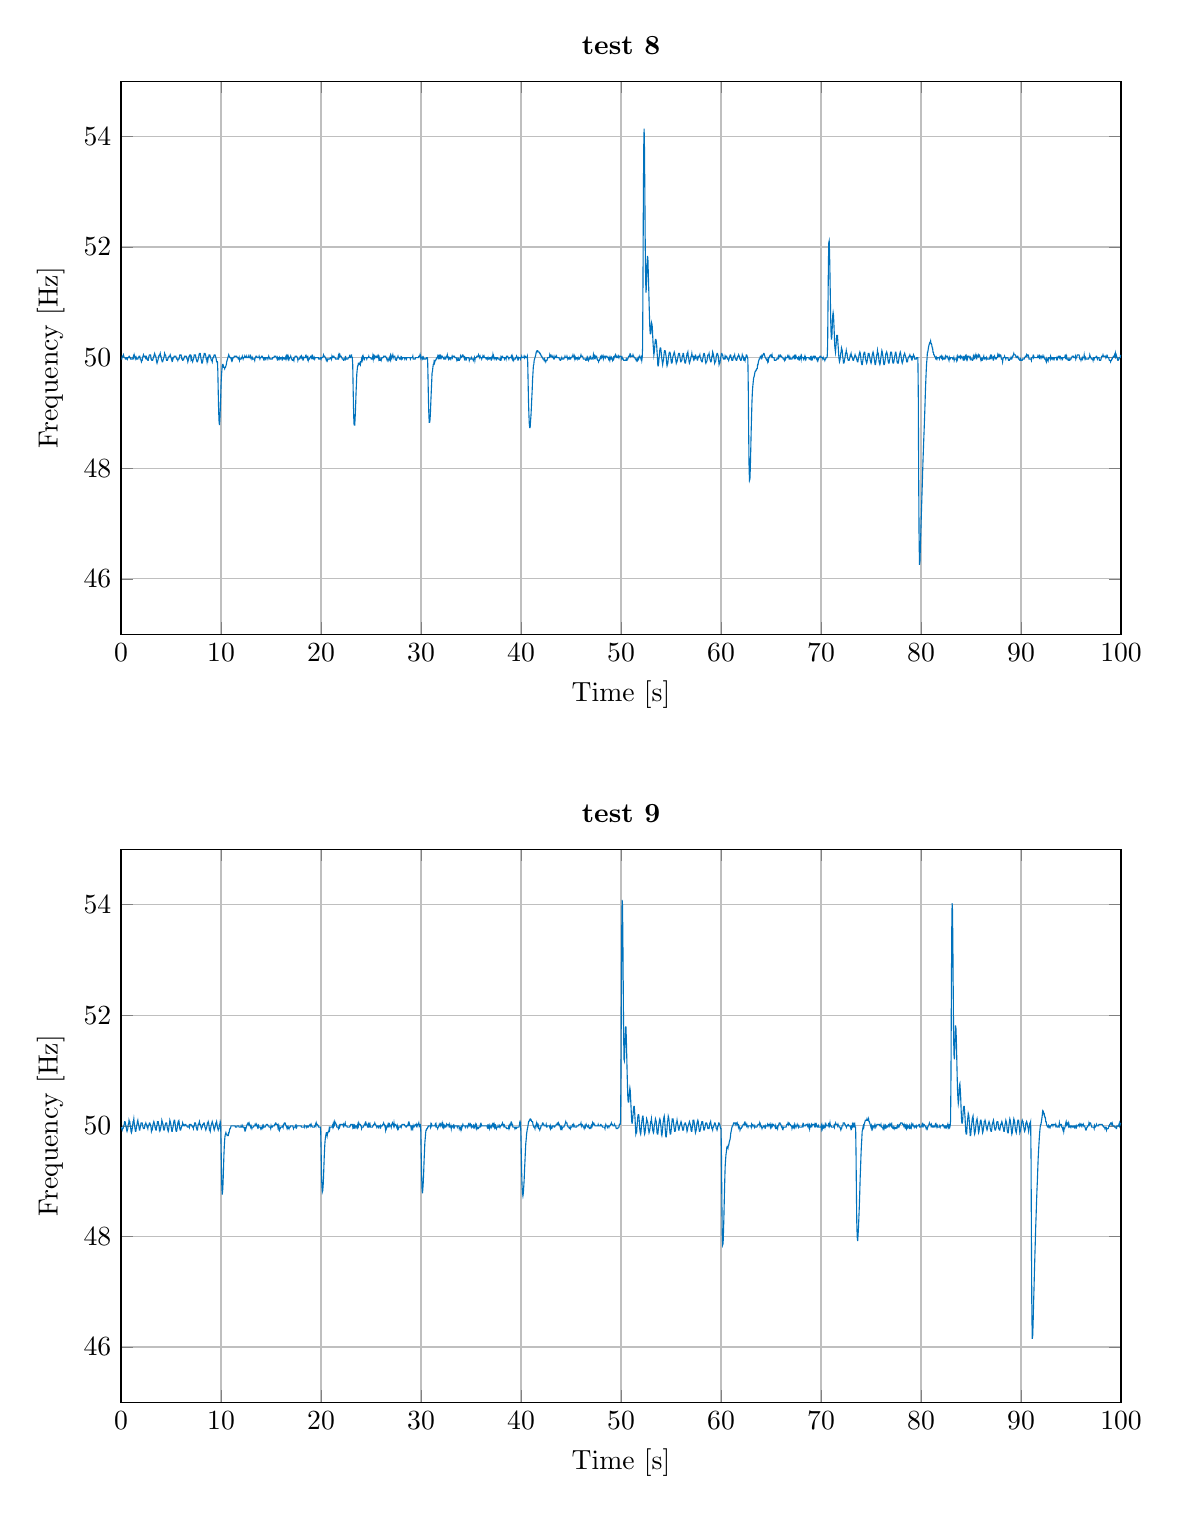
\begin{tikzpicture}

\begin{axis}[%
width=5in,
height=2.765in,
at={(1.139in,4.732in)},
scale only axis,
xmin=0,
xmax=100,
xlabel={Time [s]},
ymajorgrids,
xmajorgrids,
ymin=45,
ymax=55,
ylabel={Frequency [Hz]},
axis background/.style={fill=white},
title style={font=\bfseries},
title={test 8}
]
\addplot [color=mycolor1,solid,forget plot]
  table[row sep=crcr]{%
0.03982	49.9750124937531\\
0.07984	49.9750124937531\\
0.11986	50.0250125062531\\
0.15984	50.0250125062531\\
0.19982	50.0250125062531\\
0.2398	50.0500500500501\\
0.27976	50.0250125062531\\
0.31974	50\\
0.35974	50\\
0.39974	50\\
0.43974	49.9750124937531\\
0.47976	49.9750124937532\\
0.51978	49.9750124937531\\
0.5598	50\\
0.5998	50.0000000000001\\
0.6398	49.9750124937531\\
0.67982	50.0000000000001\\
0.71982	50\\
0.75982	50\\
0.79982	50.0250125062532\\
0.8398	50.0250125062531\\
0.87978	50\\
0.91978	50\\
0.95978	49.9750124937532\\
0.9998	49.9750124937531\\
1.03982	49.9750124937532\\
1.07984	49.9750124937532\\
1.11986	49.9750124937532\\
1.15988	49.9750124937529\\
1.1999	50\\
1.2399	50.0250125062532\\
1.27988	50\\
1.31988	50.0500500500501\\
1.35984	50.0250125062532\\
1.39982	50.025012506253\\
1.4398	50.0000000000002\\
1.4798	49.9750124937529\\
1.51982	50.0000000000002\\
1.55982	49.9750124937529\\
1.59984	49.9750124937532\\
1.63986	49.9750124937532\\
1.67988	49.9750124937532\\
1.7199	50\\
1.7599	50\\
1.7999	50.0250125062532\\
1.83988	50.025012506253\\
1.87986	50.0250125062532\\
1.91984	49.9750124937529\\
1.95986	49.9750124937532\\
1.99988	49.9500499500499\\
2.03992	49.9251123315028\\
2.07998	49.9500499500501\\
2.12002	49.9500499500501\\
2.16006	50\\
2.20006	50.0250125062532\\
2.24004	50.0500500500498\\
2.28	50.0250125062532\\
2.31998	50.0250125062532\\
2.35996	50.0250125062527\\
2.39994	50.0250125062532\\
2.43992	50\\
2.47992	50.0250125062532\\
2.5199	50.0250125062532\\
2.55988	49.9750124937529\\
2.5999	49.9750124937535\\
2.63992	49.9750124937529\\
2.67994	49.9500499500501\\
2.71998	49.9500499500496\\
2.76002	50\\
2.80002	50.0250125062532\\
2.84	50.0500500500503\\
2.87996	50.0500500500498\\
2.91992	50.0500500500503\\
2.95988	50.0500500500498\\
2.99984	49.9750124937535\\
3.03986	49.9750124937529\\
3.07988	49.9500499500501\\
3.11992	49.9500499500496\\
3.15996	49.9500499500501\\
3.2	49.9750124937529\\
3.24002	50.0000000000005\\
3.28002	50.0250125062527\\
3.32	50.0500500500503\\
3.35996	50.0751126690034\\
3.3999	50.0500500500498\\
3.43986	50.0250125062532\\
3.47984	50.0250125062532\\
3.51982	49.9750124937529\\
3.55984	49.9251123315028\\
3.5999	49.9001996007988\\
3.63998	49.9251123315028\\
3.68004	49.9500499500496\\
3.72008	49.9750124937535\\
3.7601	50.0250125062532\\
3.80008	50.0250125062527\\
3.84006	50.0500500500503\\
3.88002	50.0500500500498\\
3.91998	50.075112669004\\
3.95992	50.0250125062527\\
3.9999	50.0250125062538\\
4.03988	49.9750124937529\\
4.0799	49.9500499500496\\
4.11994	49.9251123315033\\
4.16	49.9251123315022\\
4.20006	49.9500499500496\\
4.2401	49.975012493754\\
4.28012	50\\
4.32012	50.0250125062532\\
4.3601	50.0751126690028\\
4.40004	50.0500500500503\\
4.44	50.0500500500503\\
4.47996	50.0250125062532\\
4.51994	49.9750124937529\\
4.55996	49.9500499500496\\
4.6	49.9500499500496\\
4.64004	49.9500499500507\\
4.68008	49.9750124937529\\
4.7201	50\\
4.7601	50\\
4.8001	50.0250125062532\\
4.84008	50.0250125062532\\
4.88006	50.0250125062532\\
4.92004	50.0500500500492\\
4.96	50.0250125062532\\
4.99998	50\\
5.03998	49.975012493754\\
5.08	49.9500499500496\\
5.12004	49.9750124937529\\
5.16006	49.9500499500496\\
5.2001	49.975012493754\\
5.24012	50\\
5.28012	50\\
5.32012	50.0250125062532\\
5.3601	50.0250125062532\\
5.40008	50.0250125062521\\
5.44006	50.0250125062532\\
5.48004	50.0250125062532\\
5.52002	50\\
5.56002	49.9750124937529\\
5.60004	49.975012493754\\
5.64006	49.9750124937529\\
5.68008	49.9500499500496\\
5.72012	49.9750124937529\\
5.76014	49.975012493754\\
5.80016	49.9750124937529\\
5.84018	50\\
5.88018	50.0500500500503\\
5.92014	50.0500500500492\\
5.9601	50.0500500500503\\
6.00006	50.0500500500503\\
6.04002	50.0250125062532\\
6.08	49.9750124937529\\
6.12002	49.9750124937529\\
6.16004	49.9500499500496\\
6.20008	49.9500499500507\\
6.24012	49.9750124937529\\
6.28014	49.9750124937529\\
6.32016	50\\
6.36016	50.0250125062532\\
6.40014	50.0250125062532\\
6.44012	50.0250125062532\\
6.4801	50.0250125062532\\
6.52008	50.0250125062532\\
6.56006	50\\
6.60006	49.9750124937529\\
6.64008	49.9750124937529\\
6.6801	49.9251123315033\\
6.72016	49.9500499500496\\
6.7602	49.9750124937529\\
6.80022	50.0250125062532\\
6.8402	50.0250125062532\\
6.88018	50.0500500500503\\
6.92014	50.0500500500492\\
6.9601	50.0500500500503\\
7.00006	49.9750124937529\\
7.04008	50\\
7.08008	49.9500499500507\\
7.12012	49.9500499500496\\
7.16016	49.9251123315033\\
7.20022	49.9500499500496\\
7.24026	49.9750124937529\\
7.28028	50\\
7.32028	50.0500500500503\\
7.36024	50.0500500500503\\
7.4002	50.0500500500492\\
7.44016	50.0500500500503\\
7.48012	50\\
7.52012	49.9750124937529\\
7.56014	49.9500499500507\\
7.60018	49.9251123315022\\
7.64024	49.9251123315033\\
7.6803	49.9500499500496\\
7.72034	49.9750124937529\\
7.76036	50\\
7.80036	50.0500500500503\\
7.84032	50.075112669004\\
7.88026	50.0751126690028\\
7.9202	50.075112669004\\
7.96014	50.0250125062532\\
8.00012	49.9750124937529\\
8.04014	49.9500499500507\\
8.08018	49.9001996007966\\
8.12026	49.9001996007988\\
8.16034	49.9251123315022\\
8.2004	49.9750124937551\\
8.24042	50.0250125062532\\
8.2804	50.025012506251\\
8.32038	50.075112669004\\
8.36032	50.075112669004\\
8.40026	50.075112669004\\
8.4402	50.0500500500492\\
8.48016	50.0250125062532\\
8.52014	49.9750124937529\\
8.56016	49.9750124937529\\
8.60018	49.9251123315044\\
8.64024	49.9750124937529\\
8.68026	49.9500499500485\\
8.7203	50.0000000000011\\
8.7603	49.9999999999988\\
8.8003	50.0500500500514\\
8.84026	50.0500500500492\\
8.88022	50.0500500500514\\
8.92018	50.0250125062532\\
8.96016	49.9999999999988\\
9.00016	49.9750124937529\\
9.04018	49.9500499500507\\
9.08022	49.9500499500485\\
9.12026	49.9251123315044\\
9.16032	49.9750124937529\\
9.20034	49.9999999999988\\
9.24034	50.0000000000011\\
9.28034	50.0250125062532\\
9.32032	50.0500500500492\\
9.36028	50.0500500500514\\
9.40024	50.0500500500492\\
9.4402	50.0250125062532\\
9.48018	49.9999999999988\\
9.52018	49.9750124937529\\
9.5602	49.9251123315044\\
9.60026	49.9251123315022\\
9.64032	49.9251123315022\\
9.68038	49.751243781094\\
9.72058	49.382716049383\\
9.76108	49.0436488474745\\
9.80186	48.8519785051305\\
9.8428	48.7804878048776\\
9.8838	48.8758553274684\\
9.92472	49.0677134445528\\
9.96548	49.2610837438429\\
10.00608	49.5294700346697\\
10.04646	49.6770988574268\\
10.08672	49.776007964162\\
10.1269	49.850448654038\\
10.16702	49.8753117206974\\
10.20712	49.8753117206996\\
10.24722	49.8256103637258\\
10.28736	49.825610363728\\
10.3275	49.8256103637258\\
10.36764	49.8007968127488\\
10.4078	49.825610363728\\
10.44794	49.825610363728\\
10.48808	49.850448654038\\
10.5282	49.8753117206974\\
10.5683	49.9251123315022\\
10.60836	49.9500499500507\\
10.6484	49.9750124937529\\
10.68842	49.9999999999988\\
10.72842	50.0250125062532\\
10.7684	50.0500500500514\\
10.80836	50.0250125062532\\
10.84834	50.0250125062532\\
10.88832	49.9999999999988\\
10.92832	50.0000000000011\\
10.96832	49.9999999999988\\
11.00832	49.9750124937529\\
11.04834	49.9500499500507\\
11.08838	49.9750124937529\\
11.1284	49.9500499500507\\
11.16844	49.9750124937529\\
11.20846	49.9999999999988\\
11.24846	50.0000000000011\\
11.28846	49.9999999999988\\
11.32846	50.0250125062532\\
11.36844	50.0250125062532\\
11.40842	50.0250125062532\\
11.4484	50.0250125062532\\
11.48838	50.0250125062532\\
11.52836	50.0250125062532\\
11.56834	50.0250125062532\\
11.60832	50.0000000000011\\
11.64832	49.9999999999988\\
11.68832	50.0000000000011\\
11.72832	49.9750124937529\\
11.76834	49.9750124937529\\
11.80836	49.9999999999988\\
11.84836	49.9500499500507\\
11.8884	49.9750124937529\\
11.92842	49.9750124937529\\
11.96844	49.9750124937529\\
12.00846	49.9750124937529\\
12.04848	50.0000000000011\\
12.08848	49.9999999999988\\
12.12848	50.0250125062532\\
12.16846	50.0000000000011\\
12.20846	49.9750124937529\\
12.24848	50.0000000000011\\
12.28848	49.9999999999988\\
12.32848	50.0000000000011\\
12.36848	50.0250125062532\\
12.40846	49.9999999999988\\
12.44846	50.0000000000011\\
12.48846	49.9999999999988\\
12.52846	50.0250125062532\\
12.56844	50.0000000000011\\
12.60844	49.9999999999988\\
12.64844	50.0000000000011\\
12.68844	49.9999999999988\\
12.72844	50.0250125062532\\
12.76842	50.0000000000011\\
12.80842	49.9999999999988\\
12.84842	50.0000000000011\\
12.88842	50.0250125062532\\
12.9284	49.9999999999988\\
12.9684	50.0250125062532\\
13.00838	50.0000000000011\\
13.04838	49.9999999999988\\
13.08838	49.9750124937529\\
13.1284	50.0000000000011\\
13.1684	49.9750124937529\\
13.20842	49.9750124937529\\
13.24844	49.9750124937529\\
13.28846	49.9750124937529\\
13.32848	49.9750124937529\\
13.3685	49.9500499500507\\
13.40854	49.9999999999988\\
13.44854	50.0000000000011\\
13.48854	50.0250125062532\\
13.52852	50.0250125062532\\
13.5685	50.0250125062532\\
13.60848	49.9999999999988\\
13.64848	50.0000000000011\\
13.68848	49.9999999999988\\
13.72848	50.0000000000011\\
13.76848	49.9999999999988\\
13.80848	50.0250125062532\\
13.84846	50.0000000000011\\
13.88846	49.9750124937529\\
13.92848	49.9999999999988\\
13.96848	50.0000000000011\\
14.00848	49.9999999999988\\
14.04848	50.0250125062532\\
14.08846	50.0250125062532\\
14.12844	50.0250125062532\\
14.16842	50.0000000000011\\
14.20842	49.9999999999988\\
14.24842	49.9750124937529\\
14.28844	50.0000000000011\\
14.32844	50.0000000000011\\
14.36844	49.9750124937529\\
14.40846	49.9999999999988\\
14.44846	50.0000000000011\\
14.48846	49.9750124937529\\
14.52848	49.9999999999988\\
14.56848	50.0000000000011\\
14.60848	49.9999999999988\\
14.64848	50.0000000000011\\
14.68848	49.9750124937529\\
14.7285	49.9999999999988\\
14.7685	50.0250125062532\\
14.80848	50.0000000000011\\
14.84848	49.9999999999988\\
14.88848	49.9750124937551\\
14.9285	49.9750124937529\\
14.96852	49.9750124937529\\
15.00854	49.9750124937529\\
15.04856	49.9750124937529\\
15.08858	49.9750124937529\\
15.1286	49.9750124937529\\
15.16862	50.0000000000011\\
15.20862	49.9999999999988\\
15.24862	50.0000000000011\\
15.28862	49.9999999999988\\
15.32862	50.0250125062532\\
15.3686	50.0250125062532\\
15.40858	50.0250125062532\\
15.44856	50.0250125062532\\
15.48854	50.0250125062532\\
15.52852	49.9999999999988\\
15.56852	50.0000000000011\\
15.60852	49.9750124937529\\
15.64854	50.0000000000011\\
15.68854	49.9750124937529\\
15.72856	49.9999999999988\\
15.76856	50.0000000000011\\
15.80856	49.9750124937529\\
15.84858	49.9999999999988\\
15.88858	49.9750124937529\\
15.9286	49.9750124937551\\
15.96862	50.0000000000011\\
16.00862	49.9999999999966\\
16.04862	50.0000000000011\\
16.08862	49.9750124937551\\
16.12864	49.9999999999966\\
16.16864	49.9750124937551\\
16.20866	50.0000000000011\\
16.24866	49.9999999999966\\
16.28866	50.0000000000011\\
16.32866	49.9750124937551\\
16.36868	49.9750124937507\\
16.4087	49.9750124937551\\
16.44872	50.0000000000011\\
16.48872	49.9750124937507\\
16.52874	50.0250125062532\\
16.56872	50.0000000000011\\
16.60872	50.0250125062532\\
16.6487	50.0000000000011\\
16.6887	50.0250125062532\\
16.72868	49.9750124937507\\
16.7687	50.0000000000011\\
16.8087	49.9750124937507\\
16.84872	50.0000000000011\\
16.88872	50.0000000000011\\
16.92872	50.0000000000011\\
16.96872	50.0250125062532\\
17.0087	49.9999999999966\\
17.0487	49.9750124937551\\
17.08872	49.9750124937551\\
17.12874	49.9500499500485\\
17.16878	49.9500499500485\\
17.20882	49.9500499500529\\
17.24886	49.9750124937507\\
17.28888	49.9500499500485\\
17.32892	50.0000000000011\\
17.36892	50.0000000000011\\
17.40892	50.0250125062532\\
17.4489	50.0250125062532\\
17.48888	50.0250125062532\\
17.52886	50.0250125062532\\
17.56884	50.0250125062532\\
17.60882	50.0000000000011\\
17.64882	49.9999999999966\\
17.68882	49.9500499500529\\
17.72886	49.9750124937507\\
17.76888	49.9750124937551\\
17.8089	49.9750124937507\\
17.84892	49.9750124937551\\
17.88894	50.0000000000011\\
17.92894	50.0250125062532\\
17.96892	50.0250125062532\\
18.0089	49.9999999999966\\
18.0489	50.0250125062532\\
18.08888	50.0000000000011\\
18.12888	50.0000000000011\\
18.16888	49.9750124937507\\
18.2089	50.0000000000011\\
18.2489	49.9750124937551\\
18.28892	49.9999999999966\\
18.32892	50.0000000000011\\
18.36892	50.0000000000011\\
18.40892	50.0000000000011\\
18.44892	50.0250125062532\\
18.4889	49.9999999999966\\
18.5289	50.0000000000011\\
18.5689	50.0250125062532\\
18.60888	50.0000000000011\\
18.64888	49.9750124937551\\
18.6889	49.9999999999966\\
18.7289	49.9500499500529\\
18.76894	49.9750124937507\\
18.80896	49.9750124937551\\
18.84898	49.9750124937507\\
18.889	50.0000000000011\\
18.929	50.0000000000011\\
18.969	50.0250125062532\\
19.00898	50.0250125062532\\
19.04896	50.0000000000011\\
19.08896	50.0250125062488\\
19.12894	50.0000000000011\\
19.16894	50.0250125062532\\
19.20892	50.0000000000011\\
19.24892	49.9750124937551\\
19.28894	49.9750124937507\\
19.32896	50.0000000000011\\
19.36896	49.9750124937507\\
19.40898	50.0000000000011\\
19.44898	50.0000000000011\\
19.48898	50.0000000000011\\
19.52898	49.9999999999966\\
19.56898	50.0000000000011\\
19.60898	50.0000000000011\\
19.64898	50.0000000000011\\
19.68898	49.9999999999966\\
19.72898	50.0000000000011\\
19.76898	49.9750124937551\\
19.809	49.9750124937507\\
19.84902	49.9750124937551\\
19.88904	49.9750124937507\\
19.92906	50.0000000000011\\
19.96906	50.0000000000011\\
20.00906	49.9750124937507\\
20.04908	50.0000000000011\\
20.08908	50.0000000000011\\
20.12908	50.0000000000011\\
20.16908	50.0000000000011\\
20.20908	50.0250125062532\\
20.24906	50.0500500500492\\
20.28902	50.0250125062532\\
20.329	50.0250125062532\\
20.36898	50.0250125062532\\
20.40896	49.9999999999966\\
20.44896	50.0000000000011\\
20.48896	49.9750124937551\\
20.52898	49.9500499500485\\
20.56902	49.9750124937551\\
20.60904	49.9750124937507\\
20.64906	49.9500499500485\\
20.6891	49.9750124937551\\
20.72912	49.9750124937551\\
20.76914	49.9750124937507\\
20.80916	49.9750124937551\\
20.84918	49.9750124937507\\
20.8892	49.9750124937551\\
20.92922	50.0000000000011\\
20.96922	49.9999999999966\\
21.00922	50.0000000000011\\
21.04922	49.9750124937551\\
21.08924	50.0250125062532\\
21.12922	49.9999999999966\\
21.16922	50.0000000000011\\
21.20922	50.0250125062532\\
21.2492	50.0250125062532\\
21.28918	50.0250125062532\\
21.32916	50.0000000000011\\
21.36916	50.0000000000011\\
21.40916	49.9999999999966\\
21.44916	49.9750124937551\\
21.48918	49.9750124937507\\
21.5292	49.9750124937551\\
21.56922	49.9750124937507\\
21.60924	49.9750124937551\\
21.64926	49.9750124937551\\
21.68928	49.9750124937507\\
21.7293	50.0250125062532\\
21.76928	50.0000000000011\\
21.80928	50.0500500500492\\
21.84924	50.0250125062532\\
21.88922	50.0500500500492\\
21.92918	50.0250125062532\\
21.96916	50.0250125062532\\
22.00914	50.0250125062532\\
22.04912	50.0000000000011\\
22.08912	50.0000000000011\\
22.12912	49.9750124937507\\
22.16914	49.9750124937551\\
22.20916	49.9750124937507\\
22.24918	49.9500499500529\\
22.28922	49.9500499500485\\
22.32926	49.9750124937551\\
22.36928	49.9750124937507\\
22.4093	50.0000000000011\\
22.4493	49.9750124937507\\
22.48932	50.0000000000011\\
22.52932	49.9750124937551\\
22.56934	49.9750124937507\\
22.60936	49.9750124937551\\
22.64938	49.9750124937507\\
22.6894	49.9750124937551\\
22.72942	50.0000000000011\\
22.76942	49.9999999999966\\
22.80942	50.0000000000011\\
22.84942	50.0250125062532\\
22.8894	50.0000000000011\\
22.9294	50.0000000000011\\
22.9694	50.0250125062532\\
23.00938	50.0500500500492\\
23.04934	50.0500500500492\\
23.0893	50.0000000000011\\
23.1293	50.0000000000011\\
23.1693	49.8753117206952\\
23.2094	49.4559841740848\\
23.24984	49.0918016691218\\
23.29058	48.8042947779391\\
23.33156	48.7804878048818\\
23.37256	48.7804878048776\\
23.41356	48.9236790606637\\
23.45444	49.0918016691218\\
23.49518	49.3339911198816\\
23.53572	49.5049504950473\\
23.57612	49.701789264417\\
23.61636	49.7760079641576\\
23.65654	49.8504486540402\\
23.69666	49.8504486540358\\
23.73678	49.9001996007988\\
23.77686	49.9001996007988\\
23.81694	49.8753117206996\\
23.85704	49.8753117206996\\
23.89714	49.9001996007988\\
23.93722	49.8753117206952\\
23.97732	49.9251123315022\\
24.01738	49.9251123315066\\
24.05744	49.9750124937507\\
24.09746	49.9500499500485\\
24.1375	50.0000000000011\\
24.1775	49.9750124937551\\
24.21752	50.0250125062532\\
24.2575	49.9999999999966\\
24.2975	50.0000000000011\\
24.3375	49.9750124937551\\
24.37752	50.0000000000011\\
24.41752	49.9999999999966\\
24.45752	50.0000000000011\\
24.49752	50.0000000000011\\
24.53752	50.0000000000011\\
24.57752	49.9750124937507\\
24.61754	50.0000000000011\\
24.65754	50.0000000000011\\
24.69754	49.9999999999966\\
24.73754	50.0000000000011\\
24.77754	50.0250125062532\\
24.81752	50.0000000000011\\
24.85752	50.0000000000011\\
24.89752	49.9999999999966\\
24.93752	50.0000000000011\\
24.97752	50.0000000000011\\
25.01752	49.9750124937507\\
25.05754	49.9750124937551\\
25.09756	49.9750124937551\\
25.13758	49.9750124937507\\
25.1776	50.0250125062532\\
25.21758	49.9750124937551\\
25.2576	50.0250125062532\\
25.29758	49.9999999999966\\
25.33758	50.0250125062532\\
25.37756	50.0000000000011\\
25.41756	50.0250125062532\\
25.45754	50.0250125062532\\
25.49752	50.0250125062532\\
25.5375	50.0000000000011\\
25.5775	50.0000000000011\\
25.6175	50.0250125062532\\
25.65748	49.9999999999966\\
25.69748	50.0000000000011\\
25.73748	50.0250125062532\\
25.77746	49.9750124937551\\
25.81748	49.9999999999966\\
25.85748	49.9500499500529\\
25.89752	49.9500499500485\\
25.93756	49.9500499500485\\
25.9776	49.9750124937551\\
26.01762	49.9500499500485\\
26.05766	49.9750124937551\\
26.09768	50.0000000000011\\
26.13768	49.9999999999966\\
26.17768	50.0000000000011\\
26.21768	50.0000000000011\\
26.25768	50.0250125062532\\
26.29766	50.0250125062532\\
26.33764	50.0250125062532\\
26.37762	50.0250125062532\\
26.4176	50.0250125062532\\
26.45758	50.0250125062532\\
26.49756	49.9999999999966\\
26.53756	50.0000000000011\\
26.57756	49.9750124937551\\
26.61758	49.9500499500485\\
26.65762	49.9750124937551\\
26.69764	49.9750124937507\\
26.73766	49.9750124937551\\
26.77768	49.9500499500485\\
26.81772	49.9750124937551\\
26.85774	49.9999999999966\\
26.89774	49.9750124937551\\
26.93776	50.0250125062532\\
26.97774	49.9750124937507\\
27.01776	50.0250125062532\\
27.05774	50.0000000000011\\
27.09774	50.0250125062532\\
27.13772	50.0250125062532\\
27.1777	50.0500500500492\\
27.21766	50.0000000000011\\
27.25766	50.0250125062532\\
27.29764	50.0250125062532\\
27.33762	50.0250125062532\\
27.3776	50.0250125062532\\
27.41758	49.9750124937507\\
27.4576	49.9750124937551\\
27.49762	49.9500499500485\\
27.53766	49.9500499500529\\
27.5777	49.9750124937507\\
27.61772	50.0000000000011\\
27.65772	50.0000000000011\\
27.69772	50.0250125062532\\
27.7377	50.0000000000011\\
27.7777	49.9999999999966\\
27.8177	50.0000000000011\\
27.8577	49.9750124937551\\
27.89772	49.9750124937507\\
27.93774	49.9750124937551\\
27.97776	49.9999999999966\\
28.01776	49.9750124937551\\
28.05778	50.0000000000011\\
28.09778	49.9750124937507\\
28.1378	49.9750124937551\\
28.17782	50.0000000000011\\
28.21782	49.9999999999966\\
28.25782	50.0000000000011\\
28.29782	50.0000000000011\\
28.33782	50.0000000000011\\
28.37782	49.9750124937507\\
28.41784	50.0000000000011\\
28.45784	50.0000000000011\\
28.49784	49.9999999999966\\
28.53784	49.9750124937551\\
28.57786	50.0000000000011\\
28.61786	50.0000000000011\\
28.65786	49.9999999999966\\
28.69786	50.0000000000011\\
28.73786	50.0000000000011\\
28.77786	50.0000000000011\\
28.81786	49.9999999999966\\
28.85786	50.0000000000011\\
28.89786	50.0000000000011\\
28.93786	49.9750124937507\\
28.97788	50.0000000000011\\
29.01788	50.0000000000011\\
29.05788	50.0000000000011\\
29.09788	49.9999999999966\\
29.13788	50.0000000000011\\
29.17788	50.0250125062532\\
29.21786	49.9750124937551\\
29.25788	49.9750124937507\\
29.2979	49.9750124937551\\
29.33792	49.9750124937507\\
29.37794	49.9750124937551\\
29.41796	49.9750124937507\\
29.45798	50.0000000000011\\
29.49798	50.0000000000011\\
29.53798	50.0000000000011\\
29.57798	50.0000000000011\\
29.61798	49.9999999999966\\
29.65798	50.0000000000011\\
29.69798	50.0000000000011\\
29.73798	50.0000000000011\\
29.77798	50.0250125062532\\
29.81796	50.0250125062532\\
29.85794	50.0250125062532\\
29.89792	50.0500500500492\\
29.93788	49.9999999999966\\
29.97788	50.0250125062532\\
30.01786	50.0000000000011\\
30.05786	50.0000000000011\\
30.09786	49.9750124937507\\
30.13788	50.0000000000011\\
30.17788	49.9750124937551\\
30.2179	49.9750124937507\\
30.25792	50.0000000000011\\
30.29792	49.9750124937551\\
30.33794	49.9750124937507\\
30.37796	49.9750124937551\\
30.41798	49.9750124937507\\
30.458	49.9750124937551\\
30.49802	49.9750124937507\\
30.53804	50.0000000000011\\
30.57804	50.0000000000011\\
30.61804	50.0000000000011\\
30.65804	49.9750124937507\\
30.69806	49.6524329692165\\
30.73834	49.2610837438408\\
30.77894	48.9955903968642\\
30.81976	48.828125000002\\
30.86072	48.8281249999978\\
30.90168	48.8758553274684\\
30.9426	49.0196078431405\\
30.9834	49.2125984251971\\
31.02404	49.3827160493808\\
31.06454	49.5540138751242\\
31.1049	49.726504226751\\
31.14512	49.7512437810962\\
31.18532	49.8256103637258\\
31.22546	49.8753117206996\\
31.26556	49.8753117206996\\
31.30566	49.9251123315022\\
31.34572	49.9001996007988\\
31.3858	49.9251123315022\\
31.42586	49.9500499500485\\
31.4659	49.9500499500485\\
31.50594	49.9750124937551\\
31.54596	49.9750124937551\\
31.58598	49.9999999999966\\
31.62598	50.0000000000011\\
31.66598	50.0250125062532\\
31.70596	50.0000000000011\\
31.74596	50.0250125062532\\
31.78594	50.0000000000011\\
31.82594	50.0250125062532\\
31.86592	49.9999999999966\\
31.90592	50.0250125062532\\
31.9459	50.0000000000011\\
31.9859	50.0250125062577\\
32.02588	49.9999999999922\\
32.06588	50.0250125062532\\
32.10586	50.0250125062532\\
32.14584	50.0250125062532\\
32.18582	50.0000000000011\\
32.22582	50.0000000000011\\
32.26582	49.9750124937551\\
32.30584	49.9750124937551\\
32.34586	49.9750124937463\\
32.38588	50.0000000000011\\
32.42588	49.9750124937551\\
32.4659	49.9750124937551\\
32.50592	50.0000000000011\\
32.54592	50.0250125062532\\
32.5859	50.0250125062532\\
32.62588	50.0500500500492\\
32.66584	50.0000000000011\\
32.70584	50.0000000000011\\
32.74584	49.9750124937463\\
32.78586	50.0000000000011\\
32.82586	49.9750124937551\\
32.86588	49.9750124937551\\
32.9059	50.0000000000011\\
32.9459	50.0000000000011\\
32.9859	49.9750124937463\\
33.02592	50.0000000000011\\
33.06592	50.0000000000011\\
33.10592	50.0250125062532\\
33.1459	50.0000000000011\\
33.1859	50.0250125062532\\
33.22588	50.0250125062532\\
33.26586	50.0250125062532\\
33.30584	50.0250125062532\\
33.34582	50.0250125062532\\
33.3858	50.0000000000011\\
33.4258	50.0000000000011\\
33.4658	50.0000000000011\\
33.5058	49.9999999999922\\
33.5458	49.9750124937551\\
33.58582	49.9500499500529\\
33.62586	49.9750124937551\\
33.66588	49.950049950044\\
33.70592	49.9500499500529\\
33.74596	49.9750124937551\\
33.78598	49.950049950044\\
33.82602	49.9500499500529\\
33.86606	49.9750124937551\\
33.90608	49.9750124937551\\
33.9461	50.0250125062532\\
33.98608	49.9999999999922\\
34.02608	50.0000000000011\\
34.06608	50.0250125062532\\
34.10606	50.0250125062532\\
34.14604	50.0500500500492\\
34.186	50.0500500500581\\
34.22596	50.0250125062444\\
34.26594	50.0250125062532\\
34.30592	50.0000000000011\\
34.34592	49.9750124937551\\
34.38594	50.0000000000011\\
34.42594	49.9750124937551\\
34.46596	50.0000000000011\\
34.50596	50.0000000000011\\
34.54596	49.9750124937463\\
34.58598	50.0000000000011\\
34.62598	50.0000000000011\\
34.66598	50.0000000000011\\
34.70598	50.0000000000011\\
34.74598	50.0000000000011\\
34.78598	50.0000000000011\\
34.82598	49.950049950044\\
34.86602	49.9750124937551\\
34.90604	49.9750124937551\\
34.94606	49.9750124937551\\
34.98608	49.9750124937463\\
35.0261	50.0000000000011\\
35.0661	49.9750124937551\\
35.10612	49.9750124937551\\
35.14614	49.9750124937551\\
35.18616	49.9750124937463\\
35.22618	49.9500499500529\\
35.26622	49.9750124937551\\
35.30624	49.9750124937551\\
35.34626	49.9999999999922\\
35.38626	49.9500499500529\\
35.4263	50.0000000000011\\
35.4663	50.0000000000011\\
35.5063	50.0000000000011\\
35.5463	50.0000000000011\\
35.5863	50.0250125062532\\
35.62628	50.0250125062532\\
35.66626	50.0250125062532\\
35.70624	50.0250125062532\\
35.74622	50.0500500500492\\
35.78618	50.0250125062532\\
35.82616	50.0250125062532\\
35.86614	50.0000000000011\\
35.90614	50.0250125062532\\
35.94612	49.9999999999922\\
35.98612	50.0000000000011\\
36.02612	50.0000000000011\\
36.06612	49.9750124937551\\
36.10614	50.0000000000011\\
36.14614	50.0000000000011\\
36.18614	50.0250125062532\\
36.22612	50.0000000000011\\
36.26612	49.9999999999922\\
36.30612	50.0250125062532\\
36.3461	50.0000000000011\\
36.3861	50.0000000000011\\
36.4261	50.0000000000011\\
36.4661	50.0000000000011\\
36.5061	49.9750124937551\\
36.54612	49.9750124937463\\
36.58614	50.0000000000011\\
36.62614	50.0000000000011\\
36.66614	49.9750124937551\\
36.70616	50.0000000000011\\
36.74616	49.9750124937551\\
36.78618	49.9750124937463\\
36.8262	49.9750124937551\\
36.86622	50.0000000000011\\
36.90622	50.0000000000011\\
36.94622	50.0000000000011\\
36.98622	49.9750124937551\\
37.02624	50.0000000000011\\
37.06624	49.9750124937463\\
37.10626	50.0000000000011\\
37.14626	50.0000000000011\\
37.18626	50.0500500500492\\
37.22622	50.0000000000011\\
37.26622	50.0250125062532\\
37.3062	50.0000000000011\\
37.3462	50.0000000000011\\
37.3862	49.9750124937551\\
37.42622	49.9999999999922\\
37.46622	50.0000000000011\\
37.50622	50.0000000000011\\
37.54622	49.9750124937551\\
37.58624	50.0000000000011\\
37.62624	50.0000000000011\\
37.66624	50.0000000000011\\
37.70624	49.9750124937463\\
37.74626	49.9750124937551\\
37.78628	49.9750124937551\\
37.8263	49.9750124937551\\
37.86632	49.9750124937463\\
37.90634	49.9500499500529\\
37.94638	49.9500499500529\\
37.98642	50.0000000000011\\
38.02642	49.9750124937463\\
38.06644	50.0000000000011\\
38.10644	50.0250125062532\\
38.14642	50.0250125062532\\
38.1864	50.0000000000011\\
38.2264	50.0000000000011\\
38.2664	50.0000000000011\\
38.3064	50.0000000000011\\
38.3464	49.9750124937551\\
38.38642	50.0000000000011\\
38.42642	49.9999999999922\\
38.46642	50.0000000000011\\
38.50642	49.9750124937551\\
38.54644	50.0250125062532\\
38.58642	50.0250125062532\\
38.6264	50.0250125062532\\
38.66638	50.0250125062532\\
38.70636	50.0000000000011\\
38.74636	50.0000000000011\\
38.78636	49.9750124937551\\
38.82638	49.9999999999922\\
38.86638	50.0000000000011\\
38.90638	50.0000000000011\\
38.94638	50.0000000000011\\
38.98638	50.0000000000011\\
39.02638	50.0250125062532\\
39.06636	50.0000000000011\\
39.10636	50.0250125062532\\
39.14634	49.9750124937551\\
39.18636	49.9999999999922\\
39.22636	49.9750124937551\\
39.26638	49.9500499500529\\
39.30642	49.9750124937551\\
39.34644	49.9750124937463\\
39.38646	49.9750124937551\\
39.42648	49.9750124937551\\
39.4665	50.0000000000011\\
39.5065	50.0000000000011\\
39.5465	50.0250125062532\\
39.58648	50.0000000000011\\
39.62648	49.9999999999922\\
39.66648	49.9750124937551\\
39.7065	50.0000000000011\\
39.7465	49.9750124937551\\
39.78652	50.0000000000011\\
39.82652	50.0000000000011\\
39.86652	50.0000000000011\\
39.90652	49.9999999999922\\
39.94652	49.9750124937551\\
39.98654	50.0000000000011\\
40.02654	50.0000000000011\\
40.06654	50.0250125062532\\
40.10652	50.0000000000011\\
40.14652	50.0000000000011\\
40.18652	50.0000000000011\\
40.22652	49.9999999999922\\
40.26652	50.0000000000011\\
40.30652	50.0250125062532\\
40.3465	50.0000000000011\\
40.3865	50.0250125062532\\
40.42648	50.0250125062532\\
40.46646	50.0000000000011\\
40.50646	50.0000000000011\\
40.54646	50.0000000000011\\
40.58646	50.0000000000011\\
40.62646	50.0250125062532\\
40.66644	49.9251123314978\\
40.7065	49.5785820525527\\
40.74684	49.2125984252014\\
40.78748	48.9715964740416\\
40.82832	48.8042947779433\\
40.8693	48.7329434697827\\
40.91034	48.7329434697912\\
40.95138	48.8519785051221\\
40.99232	48.947626040143\\
41.03318	49.0918016691218\\
41.07392	49.2610837438365\\
41.11452	49.4071146245118\\
41.155	49.6031746031731\\
41.19532	49.7265042267554\\
41.23554	49.8504486540358\\
41.27566	49.8753117206952\\
41.31576	49.9500499500529\\
41.3558	49.9750124937551\\
41.39582	49.9999999999922\\
41.43582	50.0250125062532\\
41.4758	50.0500500500581\\
41.51576	50.1002004007989\\
41.55568	50.1002004007989\\
41.5956	50.1253132832133\\
41.6355	50.1253132832043\\
41.6754	50.1253132832043\\
41.7153	50.1002004008078\\
41.75522	50.1002004007989\\
41.79514	50.1002004007989\\
41.83506	50.1002004008078\\
41.87498	50.0751126690017\\
41.91492	50.0751126690017\\
41.95486	50.0500500500492\\
41.99482	50.0500500500492\\
42.03478	50.0250125062532\\
42.07476	50.0250125062532\\
42.11474	50.0000000000011\\
42.15474	50.0000000000011\\
42.19474	49.9750124937551\\
42.23476	49.9750124937463\\
42.27478	49.9750124937551\\
42.3148	49.9500499500529\\
42.35484	49.9750124937551\\
42.39486	49.950049950044\\
42.4349	49.9500499500529\\
42.47494	49.9251123315066\\
42.515	49.950049950044\\
42.55504	49.9500499500529\\
42.59508	49.9500499500529\\
42.63512	49.9750124937463\\
42.67514	50.0000000000011\\
42.71514	50.0000000000011\\
42.75514	50.0000000000011\\
42.79514	50.0000000000011\\
42.83514	50.0000000000011\\
42.87514	50.0500500500492\\
42.9151	50.0250125062532\\
42.95508	50.0500500500492\\
42.99504	50.0500500500492\\
43.035	50.0250125062532\\
43.07498	50.0250125062532\\
43.11496	50.0000000000011\\
43.15496	50.0000000000011\\
43.19496	50.0250125062532\\
43.23494	50.0000000000011\\
43.27494	49.9750124937463\\
43.31496	49.9750124937551\\
43.35498	50.0000000000011\\
43.39498	50.0250125062532\\
43.43496	50.0000000000011\\
43.47496	50.0000000000011\\
43.51496	50.0000000000011\\
43.55496	50.0250125062532\\
43.59494	50.0000000000011\\
43.63494	49.9999999999922\\
43.67494	50.0000000000011\\
43.71494	50.0000000000011\\
43.75494	50.0000000000011\\
43.79494	50.0000000000011\\
43.83494	49.9750124937551\\
43.87496	49.9750124937551\\
43.91498	49.950049950044\\
43.95502	49.9500499500529\\
43.99506	49.9750124937551\\
44.03508	49.9750124937463\\
44.0751	50.0000000000011\\
44.1151	49.9750124937551\\
44.15512	49.9750124937551\\
44.19514	49.9750124937551\\
44.23516	49.9750124937463\\
44.27518	49.9750124937551\\
44.3152	50.0000000000011\\
44.3552	50.0000000000011\\
44.3952	50.0250125062532\\
44.43518	50.0000000000011\\
44.47518	50.0000000000011\\
44.51518	50.0000000000011\\
44.55518	49.9999999999922\\
44.59518	50.0250125062532\\
44.63516	50.0000000000011\\
44.67516	49.9750124937551\\
44.71518	50.0000000000011\\
44.75518	50.0000000000011\\
44.79518	49.9750124937551\\
44.8352	49.9750124937463\\
44.87522	50.0000000000011\\
44.91522	49.9750124937551\\
44.95524	49.9750124937551\\
44.99526	50.0000000000011\\
45.03526	50.0000000000011\\
45.07526	49.9999999999922\\
45.11526	50.0250125062532\\
45.15524	50.0250125062532\\
45.19522	50.0500500500581\\
45.23518	50.0250125062532\\
45.27516	50.0250125062444\\
45.31514	50.0000000000011\\
45.35514	50.0250125062532\\
45.39512	49.9750124937551\\
45.43514	50.0000000000011\\
45.47514	49.9750124937551\\
45.51516	49.9750124937551\\
45.55518	49.9999999999922\\
45.59518	50.0000000000011\\
45.63518	50.0000000000011\\
45.67518	49.9750124937551\\
45.7152	50.0000000000011\\
45.7552	49.9750124937551\\
45.79522	49.9750124937463\\
45.83524	49.9750124937551\\
45.87526	50.0000000000011\\
45.91526	50.0000000000011\\
45.95526	50.0250125062532\\
45.99524	50.0500500500492\\
46.0352	50.0250125062532\\
46.07518	50.0250125062532\\
46.11516	50.0250125062532\\
46.15514	50.0250125062532\\
46.19512	50.0000000000011\\
46.23512	49.9750124937551\\
46.27514	49.9750124937463\\
46.31516	49.9750124937551\\
46.35518	49.9750124937551\\
46.3952	49.9750124937551\\
46.43522	49.9750124937463\\
46.47524	49.9500499500529\\
46.51528	49.9500499500529\\
46.55532	49.9750124937551\\
46.59534	49.9999999999922\\
46.63534	49.9750124937551\\
46.67536	50.0000000000011\\
46.71536	49.9750124937551\\
46.75538	49.9500499500529\\
46.79542	49.9750124937463\\
46.83544	49.9750124937551\\
46.87546	50.0000000000011\\
46.91546	50.0250125062532\\
46.95544	50.0250125062532\\
46.99542	49.9750124937551\\
47.03544	49.9750124937551\\
47.07546	49.9750124937463\\
47.11548	49.9750124937551\\
47.1555	50.0000000000011\\
47.1955	50.0000000000011\\
47.2355	50.0500500500492\\
47.27546	50.0000000000011\\
47.31546	50.0250125062532\\
47.35544	50.0000000000011\\
47.39544	50.0250125062532\\
47.43542	50.0000000000011\\
47.47542	50.0250125062532\\
47.5154	50.0250125062532\\
47.55538	50.0250125062532\\
47.59536	49.9750124937463\\
47.63538	49.9750124937551\\
47.6754	49.9500499500529\\
47.71544	49.950049950044\\
47.75548	49.9251123315066\\
47.79554	49.9500499500529\\
47.83558	49.950049950044\\
47.87562	49.9750124937551\\
47.91564	49.9750124937551\\
47.95566	50.0250125062532\\
47.99564	50.0250125062532\\
48.03562	50.0000000000011\\
48.07562	50.0250125062532\\
48.1156	50.0000000000011\\
48.1556	49.9999999999922\\
48.1956	50.0250125062532\\
48.23558	49.9750124937551\\
48.2756	50.0000000000011\\
48.3156	50.0250125062532\\
48.35558	50.0250125062532\\
48.39556	50.0250125062532\\
48.43554	50.0000000000011\\
48.47554	50.0250125062532\\
48.51552	50.0250125062532\\
48.5555	50.0250125062532\\
48.59548	50.0250125062532\\
48.63546	50.0000000000011\\
48.67546	50.0000000000011\\
48.71546	50.0000000000011\\
48.75546	49.9750124937463\\
48.79548	50.0000000000011\\
48.83548	49.9750124937551\\
48.8755	49.9500499500529\\
48.91554	49.9999999999922\\
48.95554	49.9750124937551\\
48.99556	49.9750124937551\\
49.03558	50.0000000000011\\
49.07558	49.9750124937551\\
49.1156	49.9750124937463\\
49.15562	49.9500499500529\\
49.19566	49.9750124937551\\
49.23568	50.0000000000011\\
49.27568	49.9750124937551\\
49.3157	49.9999999999922\\
49.3557	50.0250125062532\\
49.39568	50.0250125062532\\
49.43566	50.0500500500581\\
49.47562	50.0250125062444\\
49.5156	50.0000000000011\\
49.5556	50.0000000000011\\
49.5956	50.0250125062532\\
49.63558	50.0000000000011\\
49.67558	50.0000000000011\\
49.71558	50.0000000000011\\
49.75558	50.0250125062532\\
49.79556	50.0000000000011\\
49.83556	50.0250125062532\\
49.87554	50.0250125062532\\
49.91552	50.0250125062532\\
49.9555	50.0250125062532\\
49.99548	50.0250125062532\\
50.03546	50.0000000000011\\
50.07546	49.9750124937551\\
50.11548	50.0000000000011\\
50.15548	49.9750124937551\\
50.1955	49.9750124937551\\
50.23552	49.9750124937463\\
50.27554	49.9500499500529\\
50.31558	49.9500499500529\\
50.35562	49.950049950044\\
50.39566	49.9500499500529\\
50.4357	49.9500499500529\\
50.47574	49.950049950044\\
50.51578	49.9750124937551\\
50.5558	49.9500499500529\\
50.59584	49.950049950044\\
50.63588	49.9750124937551\\
50.6759	49.9750124937551\\
50.71592	50.0000000000011\\
50.75592	50.0250125062532\\
50.7959	50.0250125062532\\
50.83588	50.0250125062532\\
50.87586	50.0500500500492\\
50.91582	50.0250125062532\\
50.9558	50.0500500500492\\
50.99576	50.0250125062532\\
51.03574	50.0250125062532\\
51.07572	50.0250125062532\\
51.1157	50.0250125062532\\
51.15568	50.0250125062532\\
51.19566	50.0500500500492\\
51.23562	50.0250125062532\\
51.2756	50.0250125062532\\
51.31558	50.0000000000011\\
51.35558	50.0000000000011\\
51.39558	50.0000000000011\\
51.43558	49.9750124937463\\
51.4756	49.9750124937551\\
51.51562	49.9500499500529\\
51.55566	49.9750124937551\\
51.59568	49.9750124937463\\
51.6357	49.9500499500529\\
51.67574	49.9750124937551\\
51.71576	50.0000000000011\\
51.75576	49.9750124937463\\
51.79578	50.0000000000011\\
51.83578	50.0000000000011\\
51.87578	50.0250125062532\\
51.91576	50.0000000000011\\
51.95576	50.0000000000011\\
51.99576	49.9750124937551\\
52.03578	50.0000000000011\\
52.07578	49.950049950044\\
52.11582	50.0000000000011\\
52.15582	50.1756146512828\\
52.19568	51.387461459398\\
52.2346	52.9100529100569\\
52.2724	53.8213132400429\\
52.30956	54.1418516513246\\
52.3465	53.7634408602171\\
52.3837	52.9380624669166\\
52.42148	52.0291363163353\\
52.45992	51.4138817480744\\
52.49882	51.1770726714359\\
52.5379	51.2820512820587\\
52.5769	51.519835136526\\
52.61572	51.7598343685288\\
52.65436	51.8403317781191\\
52.69294	51.7598343685383\\
52.73158	51.4933058702363\\
52.77042	51.2557662737048\\
52.80944	50.9683995922535\\
52.84868	50.7099391480743\\
52.88812	50.5050505050504\\
52.92772	50.4286434694844\\
52.96738	50.4286434694935\\
53.00704	50.5305709954512\\
53.04662	50.6329113924092\\
53.08612	50.6072874493887\\
53.12564	50.5561172901901\\
53.1652	50.4032258064554\\
53.20488	50.2512562814075\\
53.24468	50.1504513540575\\
53.28456	50.0500500500492\\
53.32452	50.1002004008078\\
53.36444	50.1756146512739\\
53.4043	50.2765208647557\\
53.44408	50.3271263210937\\
53.48382	50.3271263210847\\
53.52356	50.3018108651897\\
53.56332	50.2260170768472\\
53.60314	50.1002004007989\\
53.64306	50.0000000000011\\
53.68306	49.8504486540358\\
53.72318	49.8504486540446\\
53.7633	49.9001996007944\\
53.80338	50.0000000000011\\
53.84338	50.0500500500492\\
53.88334	50.1504513540665\\
53.92322	50.1756146512739\\
53.96308	50.1756146512828\\
54.00294	50.1253132832043\\
54.04284	50.0500500500492\\
54.0828	49.9750124937551\\
54.12282	49.9251123315066\\
54.16288	49.8753117206952\\
54.20298	49.9251123315066\\
54.24304	49.950049950044\\
54.28308	50.0250125062532\\
54.32306	50.1002004007989\\
54.36298	50.1253132832133\\
54.40288	50.1253132832043\\
54.44278	50.1002004008078\\
54.4827	50.0500500500492\\
54.52266	50.0000000000011\\
54.56266	49.9001996007944\\
54.60274	49.8504486540358\\
54.64286	49.875311720704\\
54.68296	49.9001996007944\\
54.72304	49.9750124937551\\
54.76306	50.0250125062532\\
54.80304	50.0751126690017\\
54.84298	50.1002004007989\\
54.8829	50.1002004008078\\
54.92282	50.0751126690017\\
54.96276	50.0250125062532\\
55.00274	49.9500499500529\\
55.04278	49.9001996007944\\
55.08286	49.9001996007944\\
55.12294	49.9251123315066\\
55.163	50.0000000000011\\
55.203	50.0250125062532\\
55.24298	50.0500500500492\\
55.28294	50.0751126690017\\
55.32288	50.1002004007989\\
55.3628	50.0751126690106\\
55.40274	50.0250125062532\\
55.44272	50.0000000000011\\
55.48272	49.950049950044\\
55.52276	49.9001996008032\\
55.56284	49.9251123314978\\
55.6029	49.9251123315066\\
55.64296	49.9750124937551\\
55.68298	49.9999999999922\\
55.72298	50.0500500500581\\
55.76294	50.0751126690017\\
55.80288	50.0751126690017\\
55.84282	50.0751126690017\\
55.88276	50.0250125062532\\
55.92274	49.9750124937551\\
55.96276	49.9251123314978\\
56.00282	49.9251123315066\\
56.04288	49.9500499500529\\
56.08292	49.950049950044\\
56.12296	50.0250125062532\\
56.16294	50.0250125062532\\
56.20292	50.0751126690106\\
56.24286	50.0751126690017\\
56.2828	50.0250125062532\\
56.32278	49.9750124937463\\
56.3628	49.9251123315066\\
56.40286	49.9001996007944\\
56.44294	49.9001996008032\\
56.48302	49.9500499500529\\
56.52306	49.9750124937463\\
56.56308	50.0250125062532\\
56.60306	50.0751126690106\\
56.643	50.0751126690017\\
56.68294	50.1002004007989\\
56.72286	50.0250125062532\\
56.76284	50.0000000000011\\
56.80284	49.9251123314978\\
56.8429	49.9001996008032\\
56.88298	49.9251123315066\\
56.92304	49.950049950044\\
56.96308	49.9750124937551\\
57.0031	50.0250125062532\\
57.04308	50.0250125062532\\
57.08306	50.0751126690017\\
57.123	50.0250125062532\\
57.16298	50.0250125062532\\
57.20296	50.0250125062532\\
57.24294	49.9750124937551\\
57.28296	50.0000000000011\\
57.32296	49.9750124937551\\
57.36298	49.9999999999922\\
57.40298	50.0250125062532\\
57.44296	50.0000000000011\\
57.48296	50.0250125062532\\
57.52294	50.0000000000011\\
57.56294	50.0000000000011\\
57.60294	49.9750124937551\\
57.64296	50.0000000000011\\
57.68296	49.9750124937463\\
57.72298	50.0000000000011\\
57.76298	50.0250125062532\\
57.80296	50.0250125062532\\
57.84294	50.0250125062532\\
57.88292	50.0500500500492\\
57.92288	50.0000000000011\\
57.96288	50.0000000000011\\
58.00288	49.9500499500529\\
58.04292	49.950049950044\\
58.08296	49.9251123315066\\
58.12302	49.9251123315066\\
58.16308	49.9750124937463\\
58.2031	50.0000000000011\\
58.2431	50.0500500500492\\
58.28306	50.0751126690106\\
58.323	50.0751126690017\\
58.36294	50.0500500500492\\
58.4029	50.0000000000011\\
58.4429	49.9251123314978\\
58.48296	49.9001996008032\\
58.52304	49.9251123314978\\
58.5631	49.9251123315066\\
58.60316	49.9500499500529\\
58.6432	49.9999999999922\\
58.6832	50.0500500500492\\
58.72316	50.0500500500581\\
58.76312	50.0500500500492\\
58.80308	50.0751126690017\\
58.84302	50.0250125062532\\
58.883	49.9750124937551\\
58.92302	49.950049950044\\
58.96306	49.9251123315066\\
59.00312	49.9251123314978\\
59.04318	49.9500499500529\\
59.08322	50.0250125062532\\
59.1232	50.0250125062532\\
59.16318	50.1002004007989\\
59.2031	50.0751126690106\\
59.24304	50.0500500500492\\
59.283	50.0000000000011\\
59.323	49.950049950044\\
59.36304	49.9001996008032\\
59.40312	49.9251123314978\\
59.44318	49.9251123315066\\
59.48324	49.950049950044\\
59.52328	50.0250125062532\\
59.56326	50.0500500500581\\
59.60322	50.0751126690017\\
59.64316	50.0751126690017\\
59.6831	50.0500500500492\\
59.72306	50.0250125062532\\
59.76304	49.9500499500529\\
59.80308	49.8753117206952\\
59.84318	49.9001996007944\\
59.88326	49.9001996008032\\
59.92334	49.9500499500529\\
59.96338	49.9999999999922\\
60.00338	50.0250125062532\\
60.04336	50.0751126690106\\
60.0833	50.0751126690017\\
60.12324	50.0500500500492\\
60.1632	50.0500500500492\\
60.20316	50.0000000000011\\
60.24316	49.9750124937551\\
60.28318	49.9750124937551\\
60.3232	49.9750124937463\\
60.36322	49.9750124937551\\
60.40324	50.0250125062532\\
60.44322	50.0000000000011\\
60.48322	50.0250125062532\\
60.5232	50.0250125062532\\
60.56318	50.0250125062532\\
60.60316	50.0000000000011\\
60.64316	49.9750124937551\\
60.68318	49.9750124937463\\
60.7232	49.9750124937551\\
60.76322	49.9500499500529\\
60.80326	49.9750124937551\\
60.84328	49.9999999999922\\
60.88328	50.0250125062532\\
60.92326	50.0500500500492\\
60.96322	50.0500500500581\\
61.00318	49.9999999999922\\
61.04318	50.0000000000011\\
61.08318	49.9500499500529\\
61.12322	49.9500499500529\\
61.16326	49.950049950044\\
61.2033	49.9750124937551\\
61.24332	50.0250125062532\\
61.2833	50.0250125062532\\
61.32328	50.0250125062532\\
61.36326	50.0500500500492\\
61.40322	50.0000000000011\\
61.44322	49.9750124937551\\
61.48324	49.9750124937551\\
61.52326	49.950049950044\\
61.5633	49.9500499500529\\
61.60334	49.9750124937551\\
61.64336	50.0000000000011\\
61.68336	50.0250125062532\\
61.72334	50.0250125062532\\
61.76332	50.0500500500492\\
61.80328	50.0250125062532\\
61.84326	50.0250125062532\\
61.88324	49.9750124937463\\
61.92326	49.9750124937551\\
61.96328	49.9500499500529\\
62.00332	49.9500499500529\\
62.04336	49.9750124937463\\
62.08338	50.0000000000011\\
62.12338	50.0500500500492\\
62.16334	50.0250125062532\\
62.20332	50.0250125062532\\
62.2433	50.0000000000011\\
62.2833	49.9500499500529\\
62.32334	49.950049950044\\
62.36338	49.9750124937551\\
62.4034	49.9500499500529\\
62.44344	50.0000000000011\\
62.48344	50.0000000000011\\
62.52344	50.0500500500492\\
62.5634	50.0500500500492\\
62.60336	50.0250125062532\\
62.64334	50.0000000000011\\
62.68334	49.9750124937463\\
62.72336	49.4804552201911\\
62.76378	48.6381322957206\\
62.8049	48.0076812289963\\
62.84656	47.7783086478741\\
62.88842	47.8011472275328\\
62.93026	48.0076812289963\\
62.97192	48.3325277912074\\
63.0133	48.6618004866178\\
63.0544	48.9476260401345\\
63.09526	49.2125984251928\\
63.1359	49.3827160493895\\
63.1764	49.4804552201824\\
63.21682	49.5540138751242\\
63.25718	49.6277915632817\\
63.29748	49.6524329692121\\
63.33776	49.6770988574224\\
63.37802	49.7265042267554\\
63.41824	49.7512437810962\\
63.45844	49.7512437810962\\
63.49864	49.776007964162\\
63.53882	49.776007964162\\
63.579	49.8007968127488\\
63.61916	49.8007968127488\\
63.65932	49.8753117206952\\
63.69942	49.8753117206952\\
63.73952	49.9251123315066\\
63.77958	49.9500499500529\\
63.81962	49.9750124937463\\
63.85964	49.9750124937551\\
63.89966	50.0000000000011\\
63.93966	50.0250125062532\\
63.97964	50.0250125062532\\
64.01962	49.9999999999922\\
64.05962	50.025012506271\\
64.0996	49.9999999999922\\
64.1396	50.0250125062532\\
64.17958	50.0500500500403\\
64.21954	50.0500500500581\\
64.2595	50.0751126690017\\
64.29944	50.0751126690017\\
64.33938	50.0500500500581\\
64.37934	50.0250125062355\\
64.41932	50.0000000000099\\
64.45932	50.0000000000099\\
64.49932	49.9750124937551\\
64.53934	49.9750124937551\\
64.57936	49.950049950044\\
64.6194	49.950049950044\\
64.65944	49.9251123315066\\
64.6995	49.9750124937374\\
64.73952	49.9500499500618\\
64.77956	49.9999999999922\\
64.81956	50.0000000000099\\
64.85956	50.0250125062532\\
64.89954	50.0250125062532\\
64.93952	50.0500500500403\\
64.97948	50.0500500500581\\
65.01944	50.0500500500581\\
65.0594	50.0250125062355\\
65.09938	50.0500500500581\\
65.13934	49.9999999999922\\
65.17934	50.0000000000099\\
65.21934	50.0000000000099\\
65.25934	49.9999999999922\\
65.29934	49.9999999999922\\
65.33934	49.950049950044\\
65.37938	49.9500499500618\\
65.41942	49.9500499500618\\
65.45946	49.950049950044\\
65.4995	49.950049950044\\
65.53954	49.9750124937551\\
65.57956	49.9750124937551\\
65.61958	49.9750124937551\\
65.6596	49.9750124937551\\
65.69962	49.9999999999922\\
65.73962	50.0250125062532\\
65.7796	50.0000000000099\\
65.8196	50.0250125062355\\
65.85958	50.025012506271\\
65.89956	50.0500500500403\\
65.93952	50.0500500500403\\
65.97948	50.025012506271\\
66.01946	50.0250125062355\\
66.05944	50.025012506271\\
66.09942	49.9999999999922\\
66.13942	49.9999999999922\\
66.17942	50.0000000000099\\
66.21942	49.9750124937551\\
66.25944	49.9750124937551\\
66.29946	49.9750124937551\\
66.33948	49.950049950044\\
66.37952	49.9750124937551\\
66.41954	49.9999999999922\\
66.45954	49.9750124937551\\
66.49956	49.9999999999922\\
66.53956	50.0000000000099\\
66.57956	50.0000000000099\\
66.61956	49.9999999999744\\
66.65956	50.025012506271\\
66.69954	49.9999999999922\\
66.73954	49.9999999999922\\
66.77954	50.025012506271\\
66.81952	49.9750124937551\\
66.85954	49.9750124937551\\
66.89956	49.9999999999922\\
66.93956	49.9750124937374\\
66.97958	49.9750124937551\\
67.0196	49.9750124937551\\
67.05962	49.9750124937551\\
67.09964	49.9750124937551\\
67.13966	50.0000000000099\\
67.17966	49.9999999999922\\
67.21966	50.0250125062532\\
67.25964	50.0250125062532\\
67.29962	49.9999999999922\\
67.33962	50.025012506271\\
67.3796	49.9999999999922\\
67.4196	50.0250125062532\\
67.45958	50.0000000000099\\
67.49958	50.0250125062355\\
67.53956	50.0000000000099\\
67.57956	50.0000000000099\\
67.61956	49.9999999999744\\
67.65956	49.9750124937551\\
67.69958	49.9750124937551\\
67.7396	50.0000000000099\\
67.7796	49.9750124937551\\
67.81962	50.0000000000099\\
67.85962	49.9750124937374\\
67.89964	49.9999999999922\\
67.93964	50.0000000000099\\
67.97964	50.0250125062532\\
68.01962	49.9750124937551\\
68.05964	50.0250125062532\\
68.09962	49.9999999999922\\
68.13962	50.0000000000099\\
68.17962	49.9999999999922\\
68.21962	50.0000000000099\\
68.25962	49.9750124937551\\
68.29964	49.9999999999922\\
68.33964	49.9999999999922\\
68.37964	50.025012506271\\
68.41962	49.9750124937374\\
68.45964	50.0000000000099\\
68.49964	49.9750124937551\\
68.53966	49.9999999999922\\
68.57966	50.0000000000099\\
68.61966	49.9999999999922\\
68.65966	49.9999999999922\\
68.69966	50.0000000000099\\
68.73966	49.9999999999922\\
68.77966	50.0000000000099\\
68.81966	49.9750124937374\\
68.85968	49.9750124937551\\
68.8997	49.9750124937551\\
68.93972	50.0000000000099\\
68.97972	49.9750124937551\\
69.01974	49.9999999999922\\
69.05974	49.9750124937551\\
69.09976	49.9999999999922\\
69.13976	49.9750124937551\\
69.17978	50.0000000000099\\
69.21978	49.9999999999922\\
69.25978	50.0250125062532\\
69.29976	50.0250125062532\\
69.33974	50.0000000000099\\
69.37974	50.0250125062532\\
69.41972	50.0250125062532\\
69.4597	49.9999999999922\\
69.4997	50.0000000000099\\
69.5397	49.9750124937551\\
69.57972	49.9750124937374\\
69.61974	49.9500499500618\\
69.65978	49.9750124937551\\
69.6998	49.950049950044\\
69.73984	49.9750124937551\\
69.77986	49.9999999999922\\
69.81986	50.0000000000099\\
69.85986	49.9999999999922\\
69.89986	50.0250125062532\\
69.93984	50.0250125062532\\
69.97982	50.0250125062532\\
70.0198	49.9999999999922\\
70.0598	50.0000000000099\\
70.0998	50.0000000000099\\
70.1398	49.9999999999922\\
70.1798	49.9750124937551\\
70.21982	49.9999999999922\\
70.25982	49.9750124937551\\
70.29984	49.9750124937551\\
70.33986	49.9750124937551\\
70.37988	49.950049950044\\
70.41992	49.9750124937551\\
70.45994	49.9750124937551\\
70.49996	49.9999999999922\\
70.53996	50.0000000000099\\
70.57996	49.9999999999922\\
70.61996	50.0250125062532\\
70.65994	50.2260170768562\\
70.69976	50.9943906170318\\
70.73898	51.7063081695975\\
70.77766	52.0833333333198\\
70.81606	52.1104742053296\\
70.85444	51.8941359626204\\
70.89298	51.5198351365448\\
70.9318	51.0725229826228\\
70.97096	50.6585612968624\\
71.01044	50.4032258064463\\
71.05012	50.3271263210937\\
71.08986	50.4032258064463\\
71.12954	50.5816894284421\\
71.16908	50.7614213197962\\
71.20848	50.8130081300603\\
71.24784	50.7614213197962\\
71.28724	50.6072874493978\\
71.32676	50.4286434694935\\
71.36642	50.2260170768383\\
71.40624	50.1504513540665\\
71.44612	50.1002004008078\\
71.48604	50.2008032128538\\
71.52588	50.2765208647647\\
71.56566	50.4032258064463\\
71.60534	50.4032258064463\\
71.64502	50.4032258064463\\
71.6847	50.2765208647647\\
71.72448	50.1756146512739\\
71.76434	50.0500500500581\\
71.8043	49.9750124937551\\
71.84432	49.9251123314889\\
71.88438	49.9500499500618\\
71.92442	49.9999999999922\\
71.96442	50.0751126690017\\
72.00436	50.1002004008078\\
72.04428	50.1756146512739\\
72.08414	50.1504513540665\\
72.12402	50.1253132832043\\
72.16392	50.0250125062532\\
72.2039	49.9750124937551\\
72.24392	49.9001996007944\\
72.284	49.9001996008121\\
72.32408	49.9251123314889\\
72.36414	49.9750124937551\\
72.40416	50.0000000000099\\
72.44416	50.0751126690017\\
72.4841	50.0751126690017\\
72.52404	50.1253132832043\\
72.56394	50.0751126690017\\
72.60388	50.0751126690017\\
72.64382	50.0000000000099\\
72.68382	49.9750124937374\\
72.72384	49.9500499500618\\
72.76388	49.950049950044\\
72.80392	49.9500499500618\\
72.84396	49.9750124937551\\
72.88398	49.9999999999922\\
72.92398	50.0500500500581\\
72.96394	50.0500500500403\\
73.0039	50.0751126690017\\
73.04384	50.0250125062532\\
73.08382	50.0250125062532\\
73.1238	50.0000000000099\\
73.1638	49.9750124937374\\
73.20382	49.9500499500618\\
73.24386	49.950049950044\\
73.2839	49.9750124937551\\
73.32392	49.9999999999922\\
73.36392	50.0250125062532\\
73.4039	50.0500500500581\\
73.44386	50.0250125062532\\
73.48384	50.0250125062532\\
73.52382	49.9999999999922\\
73.56382	49.9750124937551\\
73.60384	49.950049950044\\
73.64388	49.9251123315066\\
73.68394	49.9251123315066\\
73.724	49.9750124937551\\
73.76402	50.0000000000099\\
73.80402	50.0500500500403\\
73.84398	50.0751126690017\\
73.88392	50.1002004008078\\
73.92384	50.0751126690017\\
73.96378	50.0250125062532\\
74.00376	49.950049950044\\
74.0438	49.9001996007944\\
74.08388	49.875311720704\\
74.12398	49.875311720704\\
74.16408	49.9251123314889\\
74.20414	49.9750124937551\\
74.24416	50.0500500500581\\
74.28412	50.0751126690017\\
74.32406	50.1002004008078\\
74.36398	50.10020040079\\
74.4039	50.0500500500581\\
74.44386	49.9750124937551\\
74.48388	49.950049950044\\
74.52392	49.9251123315066\\
74.56398	49.9001996007944\\
74.60406	49.9251123315066\\
74.64412	49.9750124937551\\
74.68414	50.0250125062532\\
74.72412	50.0751126690017\\
74.76406	50.0751126690017\\
74.804	50.0751126690017\\
74.84394	50.0250125062532\\
74.88392	50.0000000000099\\
74.92392	49.950049950044\\
74.96396	49.9251123315066\\
75.00402	49.9001996007944\\
75.0441	49.9251123315066\\
75.08416	49.9999999999922\\
75.12416	50.0500500500581\\
75.16412	50.0751126690017\\
75.20406	50.10020040079\\
75.24398	50.0751126690017\\
75.28392	50.025012506271\\
75.3239	49.9750124937374\\
75.36392	49.9251123315066\\
75.40398	49.875311720704\\
75.44408	49.875311720704\\
75.48418	49.9251123314889\\
75.52424	49.9750124937551\\
75.56426	50.0500500500581\\
75.60422	50.0500500500403\\
75.64418	50.1253132832043\\
75.68408	50.0751126690017\\
75.72402	50.0751126690195\\
75.76396	49.9999999999922\\
75.80396	49.9251123315066\\
75.84402	49.9001996007944\\
75.8841	49.875311720704\\
75.9242	49.9001996007944\\
75.96428	49.9750124937551\\
76.0043	50.0250125062532\\
76.04428	50.0751126690017\\
76.08422	50.1253132832043\\
76.12412	50.1002004008078\\
76.16404	50.0500500500581\\
76.204	49.9999999999922\\
76.244	49.9251123315066\\
76.28406	49.8753117206863\\
76.32416	49.875311720704\\
76.36426	49.9001996007944\\
76.40434	49.950049950044\\
76.44438	50.0000000000099\\
76.48438	50.0751126690017\\
76.52432	50.0751126690017\\
76.56426	50.1002004008078\\
76.60418	50.0751126690017\\
76.64412	50.0500500500403\\
76.68408	49.9750124937551\\
76.7241	49.9251123315066\\
76.76416	49.9001996007944\\
76.80424	49.9001996008121\\
76.84432	49.950049950044\\
76.88436	49.9750124937551\\
76.92438	50.0500500500403\\
76.96434	50.1002004008078\\
77.00426	50.1002004008078\\
77.04418	50.10020040079\\
77.0841	50.0500500500581\\
77.12406	49.9999999999922\\
77.16406	49.9251123315066\\
77.20412	49.9001996007944\\
77.2442	49.9001996007944\\
77.28428	49.9251123315066\\
77.32434	49.9750124937551\\
77.36436	50.0250125062532\\
77.40434	50.0500500500581\\
77.4443	50.10020040079\\
77.48422	50.1002004008078\\
77.52414	50.0500500500403\\
77.5641	50.0000000000099\\
77.6041	49.9251123315066\\
77.64416	49.9001996007944\\
77.68424	49.9001996007944\\
77.72432	49.9001996007944\\
77.7644	49.9500499500618\\
77.80444	49.9999999999922\\
77.84444	50.0500500500581\\
77.8844	50.0751126690017\\
77.92434	50.10020040079\\
77.96426	50.0751126690195\\
78.0042	50.0250125062532\\
78.04418	49.9750124937551\\
78.0842	49.9251123314889\\
78.12426	49.9001996008121\\
78.16434	49.9251123314889\\
78.2044	49.9500499500618\\
78.24444	49.9999999999922\\
78.28444	50.0500500500581\\
78.3244	50.0500500500403\\
78.36436	50.0751126690017\\
78.4043	50.0500500500581\\
78.44426	50.0250125062532\\
78.48424	49.9999999999922\\
78.52424	49.9750124937551\\
78.56426	49.9251123315066\\
78.60432	49.9251123315066\\
78.64438	49.9251123314889\\
78.68444	49.9750124937551\\
78.72446	50.0000000000099\\
78.76446	49.9999999999922\\
78.80446	50.0250125062532\\
78.84444	50.0250125062532\\
78.88442	50.0500500500581\\
78.92438	50.0250125062532\\
78.96436	50.0250125062532\\
79.00434	49.9999999999922\\
79.04434	49.9750124937551\\
79.08436	49.9999999999922\\
79.12436	49.9750124937551\\
79.16438	50.0000000000099\\
79.20438	50.0250125062532\\
79.24436	50.0500500500581\\
79.28432	50.0250125062355\\
79.3243	50.025012506271\\
79.36428	49.9750124937374\\
79.4043	49.9750124937551\\
79.44432	49.9750124937551\\
79.48434	49.9750124937551\\
79.52436	49.9750124937551\\
79.56438	49.9999999999922\\
79.60438	50.0000000000099\\
79.64438	49.9999999999922\\
79.68438	50.0000000000099\\
79.72438	49.3827160493722\\
79.76488	47.8240076518397\\
79.8067	46.6853408029898\\
79.84954	46.2534690101787\\
79.89278	46.3177396942958\\
79.93596	46.5983224603967\\
79.97888	46.8384074941491\\
80.02158	47.10315591144\\
80.06404	47.3484848484933\\
80.10628	47.5963826749077\\
80.1483	47.8468899521589\\
80.1901	48.1000481000525\\
80.23168	48.3091787439496\\
80.27308	48.5201358563856\\
80.3143	48.7092060399396\\
80.35536	48.9236790606637\\
80.39624	49.1400491400479\\
80.43694	49.3827160493895\\
80.47744	49.5785820525527\\
80.51778	49.7512437810962\\
80.55798	49.9001996007944\\
80.59806	49.9750124937551\\
80.63808	50.1002004008078\\
80.678	50.10020040079\\
80.71792	50.1504513540665\\
80.7578	50.2008032128538\\
80.79764	50.2260170768383\\
80.83746	50.2512562814075\\
80.87726	50.2765208647647\\
80.91704	50.2765208647467\\
80.95682	50.3018108651897\\
80.99658	50.2512562814255\\
81.03638	50.2512562813896\\
81.07618	50.2260170768562\\
81.116	50.1756146512739\\
81.15586	50.1756146512739\\
81.19572	50.1002004008078\\
81.23564	50.1002004008078\\
81.27556	50.0500500500403\\
81.31552	50.0500500500581\\
81.35548	50.0250125062532\\
81.39546	50.0250125062532\\
81.43544	49.9999999999922\\
81.47544	49.9750124937551\\
81.51546	49.9750124937551\\
81.55548	50.0000000000099\\
81.59548	49.9750124937551\\
81.6355	49.9999999999922\\
81.6755	49.9999999999922\\
81.7155	50.0000000000099\\
81.7555	49.9999999999922\\
81.7955	49.9999999999922\\
81.8355	49.9750124937551\\
81.87552	50.0000000000099\\
81.91552	50.0250125062532\\
81.9555	50.0250125062532\\
81.99548	50.0250125062532\\
82.03546	49.9999999999922\\
82.07546	50.0250125062532\\
82.11544	50.0000000000099\\
82.15544	49.9750124937551\\
82.19546	49.9999999999922\\
82.23546	49.9750124937551\\
82.27548	49.9750124937551\\
82.3155	49.9750124937551\\
82.35552	49.9750124937551\\
82.39554	49.9999999999922\\
82.43554	50.0250125062532\\
82.47552	50.0000000000099\\
82.51552	50.0250125062355\\
82.5555	50.025012506271\\
82.59548	50.0250125062355\\
82.63546	50.025012506271\\
82.67544	49.9999999999922\\
82.71544	49.9750124937551\\
82.75546	49.9750124937551\\
82.79548	49.950049950044\\
82.83552	49.9999999999922\\
82.87552	49.9750124937551\\
82.91554	49.9750124937551\\
82.95556	50.0000000000099\\
82.99556	49.9999999999922\\
83.03556	49.9999999999922\\
83.07556	50.0000000000099\\
83.11556	50.0000000000099\\
83.15556	49.9750124937374\\
83.19558	49.9750124937551\\
83.2356	49.9750124937551\\
83.27562	49.9999999999922\\
83.31562	49.9500499500618\\
83.35566	49.9750124937551\\
83.39568	49.9750124937551\\
83.4357	49.9750124937374\\
83.47572	49.9750124937551\\
83.51574	49.9750124937551\\
83.55576	49.9500499500618\\
83.5958	49.9999999999922\\
83.6358	49.9750124937551\\
83.67582	50.0250125062532\\
83.7158	49.9999999999922\\
83.7558	50.0000000000099\\
83.7958	49.9999999999922\\
83.8358	50.0250125062532\\
83.87578	50.0250125062532\\
83.91576	50.0000000000099\\
83.95576	50.0250125062532\\
83.99574	49.9999999999922\\
84.03574	50.0250125062532\\
84.07572	50.0250125062532\\
84.1157	50.0000000000099\\
84.1557	49.9999999999922\\
84.1957	49.9750124937551\\
84.23572	49.9999999999922\\
84.27572	49.9750124937551\\
84.31574	50.0000000000099\\
84.35574	49.9750124937551\\
84.39576	49.9999999999922\\
84.43576	50.0250125062532\\
84.47574	49.9999999999922\\
84.51574	50.025012506271\\
84.55572	49.9750124937374\\
84.59574	50.0000000000099\\
84.63574	49.9750124937551\\
84.67576	50.0250125062532\\
84.71574	50.0250125062532\\
84.75572	50.0250125062532\\
84.7957	50.0250125062532\\
84.83568	49.9999999999922\\
84.87568	50.0000000000099\\
84.91568	49.9750124937374\\
84.9557	50.0000000000099\\
84.9957	49.9750124937551\\
85.03572	49.9750124937551\\
85.07574	49.9750124937374\\
85.11576	49.9500499500618\\
85.1558	49.950049950044\\
85.19584	49.9750124937551\\
85.23586	50.0250125062532\\
85.27584	50.0000000000099\\
85.31584	50.0250125062355\\
85.35582	50.0000000000099\\
85.39582	50.0250125062532\\
85.4358	50.0250125062532\\
85.47578	50.0500500500403\\
85.51574	50.0000000000099\\
85.55574	50.0250125062532\\
85.59572	49.9999999999922\\
85.63572	50.0250125062532\\
85.6757	50.0250125062532\\
85.71568	50.0500500500581\\
85.75564	50.0250125062532\\
85.79562	50.0500500500403\\
85.83558	50.0500500500581\\
85.87554	50.0250125062532\\
85.91552	49.9999999999922\\
85.95552	49.9750124937551\\
85.99554	49.9500499500618\\
86.03558	49.9750124937551\\
86.0756	49.950049950044\\
86.11564	49.950049950044\\
86.15568	49.9750124937551\\
86.1957	50.0000000000099\\
86.2357	49.9999999999922\\
86.2757	50.0250125062532\\
86.31568	49.9750124937551\\
86.3557	49.9750124937551\\
86.39572	49.9999999999922\\
86.43572	50.0000000000099\\
86.47572	49.9999999999922\\
86.51572	49.9750124937551\\
86.55574	49.9999999999922\\
86.59574	49.9750124937551\\
86.63576	49.9750124937551\\
86.67578	49.9750124937551\\
86.7158	49.9750124937551\\
86.75582	49.9750124937551\\
86.79584	49.9750124937551\\
86.83586	49.9750124937551\\
86.87588	49.9999999999922\\
86.91588	50.0250125062532\\
86.95586	49.9999999999922\\
86.99586	50.025012506271\\
87.03584	49.9999999999922\\
87.07584	50.0250125062532\\
87.11582	49.9999999999922\\
87.15582	50.0000000000099\\
87.19582	49.9750124937551\\
87.23584	49.9999999999922\\
87.27584	49.9750124937551\\
87.31586	49.9999999999922\\
87.35586	50.0250125062532\\
87.39584	50.0000000000099\\
87.43584	49.9999999999922\\
87.47584	49.9750124937551\\
87.51586	49.9750124937551\\
87.55588	49.9999999999922\\
87.59588	50.0000000000099\\
87.63588	49.9999999999922\\
87.67588	50.0500500500581\\
87.71584	50.0250125062532\\
87.75582	50.0250125062532\\
87.7958	50.0500500500403\\
87.83576	50.025012506271\\
87.87574	50.0250125062355\\
87.91572	50.0500500500581\\
87.95568	50.0500500500581\\
87.99564	50.0250125062355\\
88.03562	49.9750124937551\\
88.07564	49.9750124937551\\
88.11566	49.9750124937551\\
88.15568	49.9251123315066\\
88.19574	49.9750124937551\\
88.23576	49.9999999999922\\
88.27576	50.0000000000099\\
88.31576	49.9999999999922\\
88.35576	50.0250125062532\\
88.39574	50.0000000000099\\
88.43574	49.9999999999922\\
88.47574	49.9750124937551\\
88.51576	49.9999999999922\\
88.55576	50.0000000000099\\
88.59576	49.9999999999922\\
88.63576	50.0000000000099\\
88.67576	49.9999999999922\\
88.71576	49.9750124937551\\
88.75578	49.950049950044\\
88.79582	49.9500499500618\\
88.83586	49.950049950044\\
88.8759	49.9750124937551\\
88.91592	49.9750124937551\\
88.95594	49.9750124937551\\
88.99596	49.9999999999922\\
89.03596	49.9750124937551\\
89.07598	49.9750124937551\\
89.116	49.9999999999922\\
89.156	50.0250125062532\\
89.19598	50.0250125062532\\
89.23596	50.0500500500581\\
89.27592	50.0751126690017\\
89.31586	50.0500500500403\\
89.35582	50.0500500500581\\
89.39578	50.0500500500581\\
89.43574	50.0500500500403\\
89.4757	50.0250125062532\\
89.51568	50.0000000000099\\
89.55568	49.9999999999922\\
89.59568	50.0000000000099\\
89.63568	50.0250125062355\\
89.67566	50.025012506271\\
89.71564	49.9999999999922\\
89.75564	49.9750124937551\\
89.79566	49.9750124937551\\
89.83568	49.9750124937551\\
89.8757	49.950049950044\\
89.91574	49.950049950044\\
89.95578	49.9750124937551\\
89.9958	49.9500499500618\\
90.03584	49.950049950044\\
90.07588	49.950049950044\\
90.11592	49.950049950044\\
90.15596	49.9750124937551\\
90.19598	49.9750124937551\\
90.236	49.9750124937551\\
90.27602	49.9750124937551\\
90.31604	49.9750124937551\\
90.35606	49.9999999999922\\
90.39606	50.0000000000099\\
90.43606	50.0250125062532\\
90.47604	50.0250125062532\\
90.51602	50.0250125062532\\
90.556	50.0500500500403\\
90.59596	50.0250125062532\\
90.63594	50.0500500500581\\
90.6759	50.0500500500403\\
90.71586	50.0500500500581\\
90.75582	50.0250125062532\\
90.7958	49.9750124937551\\
90.83582	49.9750124937551\\
90.87584	49.9750124937551\\
90.91586	49.9750124937551\\
90.95588	49.9750124937374\\
90.9959	49.9750124937551\\
91.03592	49.9500499500618\\
91.07596	49.9999999999922\\
91.11596	49.9999999999922\\
91.15596	50.0000000000099\\
91.19596	50.0250125062532\\
91.23594	49.9999999999922\\
91.27594	50.0250125062532\\
91.31592	50.0000000000099\\
91.35592	49.9999999999922\\
91.39592	50.0000000000099\\
91.43592	49.9999999999922\\
91.47592	49.9999999999922\\
91.51592	50.0000000000099\\
91.55592	49.9999999999922\\
91.59592	50.0000000000099\\
91.63592	49.9999999999922\\
91.67592	50.0250125062532\\
91.7159	50.0000000000099\\
91.7559	49.9999999999922\\
91.7959	50.0250125062532\\
91.83588	50.0000000000099\\
91.87588	50.0250125062532\\
91.91586	49.9999999999922\\
91.95586	50.0250125062532\\
91.99584	50.0250125062532\\
92.03582	50.0250125062532\\
92.0758	49.9999999999922\\
92.1158	50.0250125062532\\
92.15578	50.0000000000099\\
92.19578	49.9999999999922\\
92.23578	50.0000000000099\\
92.27578	50.0250125062532\\
92.31576	49.9999999999922\\
92.35576	49.9750124937551\\
92.39578	49.9750124937551\\
92.4358	49.9750124937551\\
92.47582	49.950049950044\\
92.51586	49.9750124937551\\
92.55588	49.9251123315066\\
92.59594	49.950049950044\\
92.63598	49.9750124937551\\
92.676	49.9750124937551\\
92.71602	49.950049950044\\
92.75606	50.0000000000099\\
92.79606	49.9999999999922\\
92.83606	50.0000000000099\\
92.87606	49.9999999999922\\
92.91606	49.9750124937551\\
92.95608	50.0250125062532\\
92.99606	49.9999999999922\\
93.03606	49.9750124937551\\
93.07608	49.9750124937551\\
93.1161	50.0000000000099\\
93.1561	49.9999999999922\\
93.1961	49.9750124937551\\
93.23612	49.9999999999922\\
93.27612	50.0000000000099\\
93.31612	49.9750124937551\\
93.35614	49.9999999999922\\
93.39614	50.0000000000099\\
93.43614	49.9999999999922\\
93.47614	49.9999999999922\\
93.51614	50.0000000000099\\
93.55614	49.9750124937551\\
93.59616	49.9999999999922\\
93.63616	49.9750124937551\\
93.67618	50.0000000000099\\
93.71618	49.9999999999922\\
93.75618	50.0250125062532\\
93.79616	50.0250125062532\\
93.83614	49.9999999999922\\
93.87614	50.0250125062532\\
93.91612	50.0250125062532\\
93.9561	50.0000000000099\\
93.9961	49.9750124937551\\
94.03612	49.9999999999922\\
94.07612	50.0000000000099\\
94.11612	49.9999999999922\\
94.15612	49.9750124937551\\
94.19614	49.9999999999922\\
94.23614	50.0000000000099\\
94.27614	49.9999999999922\\
94.31614	50.0000000000099\\
94.35614	49.9999999999922\\
94.39614	50.0250125062532\\
94.43612	50.0000000000099\\
94.47612	50.0250125062532\\
94.5161	49.9999999999922\\
94.5561	50.0250125062532\\
94.59608	49.9750124937551\\
94.6361	49.9750124937551\\
94.67612	49.9750124937551\\
94.71614	49.950049950044\\
94.75618	49.950049950044\\
94.79622	49.9750124937551\\
94.83624	49.9500499500618\\
94.87628	49.950049950044\\
94.91632	49.9750124937551\\
94.95634	49.9750124937551\\
94.99636	49.9750124937551\\
95.03638	49.9999999999922\\
95.07638	49.9999999999922\\
95.11638	50.0250125062532\\
95.15636	50.0250125062532\\
95.19634	50.0250125062532\\
95.23632	50.0250125062532\\
95.2763	50.0000000000099\\
95.3163	49.9999999999922\\
95.3563	50.0000000000099\\
95.3963	49.9999999999922\\
95.4363	50.0250125062532\\
95.47628	49.9750124937551\\
95.5163	49.9999999999922\\
95.5563	50.0000000000099\\
95.5963	50.0250125062532\\
95.63628	50.0500500500581\\
95.67624	50.0500500500403\\
95.7162	50.0500500500581\\
95.75616	50.0500500500403\\
95.79612	50.0500500500581\\
95.83608	50.0250125062532\\
95.87606	49.9750124937551\\
95.91608	49.9750124937374\\
95.9561	49.9750124937551\\
95.99612	49.9500499500618\\
96.03616	49.9750124937551\\
96.07618	49.9750124937374\\
96.1162	50.0000000000099\\
96.1562	49.9750124937551\\
96.19622	49.9999999999922\\
96.23622	50.0000000000099\\
96.27622	49.9999999999922\\
96.31622	50.0500500500581\\
96.35618	49.9999999999922\\
96.39618	49.9750124937551\\
96.4362	49.9999999999922\\
96.4762	49.9750124937551\\
96.51622	49.9750124937551\\
96.55624	49.9750124937551\\
96.59626	49.9750124937551\\
96.63628	49.9750124937551\\
96.6763	49.9750124937551\\
96.71632	49.9750124937551\\
96.75634	49.9750124937374\\
96.79636	50.0000000000099\\
96.83636	49.9999999999922\\
96.87636	50.0500500500581\\
96.91632	50.0250125062532\\
96.9563	49.9999999999922\\
96.9963	50.0000000000099\\
97.0363	49.9750124937551\\
97.07632	49.9750124937551\\
97.11634	49.9750124937374\\
97.15636	49.9750124937551\\
97.19638	49.9500499500618\\
97.23642	49.9999999999922\\
97.27642	50.0000000000099\\
97.31642	49.9750124937374\\
97.35644	50.0000000000099\\
97.39644	49.9999999999922\\
97.43644	50.0000000000099\\
97.47644	49.9999999999922\\
97.51644	50.0250125062532\\
97.55642	50.0250125062532\\
97.5964	50.0000000000099\\
97.6364	49.9750124937551\\
97.67642	49.9999999999922\\
97.71642	49.9999999999922\\
97.75642	50.0000000000099\\
97.79642	49.9999999999922\\
97.83642	49.9500499500618\\
97.87646	49.950049950044\\
97.9165	49.950049950044\\
97.95654	49.9500499500618\\
97.99658	49.9750124937374\\
98.0366	50.0000000000099\\
98.0766	50.0250125062532\\
98.11658	50.0250125062532\\
98.15656	50.0250125062532\\
98.19654	50.0500500500403\\
98.2365	50.0250125062532\\
98.27648	50.0250125062532\\
98.31646	50.0250125062532\\
98.35644	50.0250125062532\\
98.39642	50.0250125062532\\
98.4364	50.0250125062532\\
98.47638	50.0000000000099\\
98.51638	50.0250125062532\\
98.55636	49.9999999999922\\
98.59636	50.0000000000099\\
98.63636	50.0250125062532\\
98.67634	49.9999999999922\\
98.71634	50.0000000000099\\
98.75634	49.9999999999922\\
98.79634	49.9750124937551\\
98.83636	49.950049950044\\
98.8764	49.9500499500618\\
98.91644	49.950049950044\\
98.95648	49.9251123315066\\
98.99654	49.950049950044\\
99.03658	49.950049950044\\
99.07662	49.9750124937551\\
99.11664	49.9750124937551\\
99.15666	50.0000000000099\\
99.19666	49.9999999999922\\
99.23666	50.0250125062532\\
99.27664	50.0250125062532\\
99.31662	50.0250125062532\\
99.3566	50.0500500500581\\
99.39656	50.0250125062532\\
99.43654	50.0751126690017\\
99.47648	50.0250125062532\\
99.51646	50.0500500500403\\
99.55642	50.0250125062532\\
99.5964	50.0000000000099\\
99.6364	49.9750124937551\\
99.67642	49.950049950044\\
99.71646	49.950049950044\\
99.7565	49.9750124937551\\
99.79652	49.9750124937551\\
99.83654	49.9999999999922\\
99.87654	50.0000000000099\\
99.91654	49.9999999999922\\
99.95654	50.0500500500581\\
};
\end{axis}

\begin{axis}[%
width=5in,
height=2.765in,
at={(1.139in,0.891in)},
scale only axis,
xmin=0,
xmax=100,
xlabel={Time [s]},
ymajorgrids,
xmajorgrids,
ymin=45,
ymax=55,
ylabel={Frequency [Hz]},
axis background/.style={fill=white},
title style={font=\bfseries},
title={test 9}
]
\addplot [color=mycolor1,solid,forget plot]
  table[row sep=crcr]{%
0.03998	49.9750124937531\\
0.08	49.9500499500499\\
0.12004	49.9251123315027\\
0.1601	49.95004995005\\
0.20014	49.95004995005\\
0.24018	49.9750124937532\\
0.2802	50\\
0.3202	50.0250125062532\\
0.36018	50.0751126690035\\
0.40012	50.0751126690035\\
0.44006	50.0500500500501\\
0.48002	50\\
0.52002	49.9750124937531\\
0.56004	49.9251123315028\\
0.6001	49.9001996007984\\
0.64018	49.9251123315028\\
0.68024	49.95004995005\\
0.72028	50.0250125062531\\
0.76026	50.0250125062531\\
0.80024	50.1002004008017\\
0.84016	50.0751126690035\\
0.8801	50.0751126690034\\
0.92004	50.0000000000001\\
0.96004	49.9750124937531\\
1.00006	49.9001996007985\\
1.04014	49.8753117206982\\
1.08024	49.9001996007983\\
1.12032	49.9500499500501\\
1.16036	50\\
1.20036	50.0751126690034\\
1.2403	50.0751126690037\\
1.28024	50.125313283208\\
1.32014	50.0500500500501\\
1.3601	50\\
1.4001	49.9500499500499\\
1.44014	49.9001996007985\\
1.48022	49.9001996007985\\
1.5203	49.9500499500499\\
1.56034	50\\
1.60034	50.0250125062532\\
1.64032	50.0751126690034\\
1.68026	50.1002004008017\\
1.72018	50.0500500500501\\
1.76014	50.025012506253\\
1.80012	49.9750124937532\\
1.84014	49.9251123315028\\
1.8802	49.9251123315028\\
1.92026	49.9750124937532\\
1.96028	50.0000000000002\\
2.00028	50.0500500500498\\
2.04024	50.0500500500503\\
2.0802	50.0500500500498\\
2.12016	50.0500500500503\\
2.16012	50\\
2.20012	49.9750124937529\\
2.24014	49.9500499500501\\
2.28018	49.9500499500496\\
2.32022	49.9500499500501\\
2.36026	49.9750124937529\\
2.40028	50.0250125062532\\
2.44026	50.0250125062532\\
2.48024	50.0500500500498\\
2.5202	50.0250125062532\\
2.56018	50.0250125062532\\
2.60016	49.9750124937529\\
2.64018	49.9750124937535\\
2.6802	49.9500499500501\\
2.72024	50\\
2.76024	50\\
2.80024	50.0250125062527\\
2.84022	50.0500500500503\\
2.88018	50.0500500500498\\
2.92014	50.0250125062532\\
2.96012	50\\
3.00012	49.9750124937535\\
3.04014	49.9001996007983\\
3.08022	49.9251123315028\\
3.12028	49.9251123315028\\
3.16034	49.9750124937529\\
3.20036	50.0250125062532\\
3.24034	50.0500500500503\\
3.2803	50.0751126690034\\
3.32024	50.0500500500498\\
3.3602	50.0250125062532\\
3.40018	49.9750124937535\\
3.4402	49.9500499500496\\
3.48024	49.9251123315028\\
3.5203	49.9251123315028\\
3.56036	50\\
3.60036	50\\
3.64036	50.075112669004\\
3.6803	50.0751126690034\\
3.72024	50.0751126690034\\
3.76018	50.0250125062532\\
3.80016	50\\
3.84016	49.9251123315028\\
3.88022	49.9500499500496\\
3.92026	49.9251123315028\\
3.96032	49.9500499500501\\
4.00036	50\\
4.04036	50.0250125062532\\
4.08034	50.1002004008011\\
4.12026	50.075112669004\\
4.1602	50.0500500500503\\
4.20016	50.0250125062532\\
4.24014	49.9500499500496\\
4.28018	49.9251123315033\\
4.32024	49.9251123315022\\
4.3603	49.9500499500496\\
4.40034	50\\
4.44034	50.0250125062532\\
4.48032	50.0500500500503\\
4.52028	50.0500500500503\\
4.56024	50.0500500500503\\
4.6002	50\\
4.6402	49.9500499500496\\
4.68024	49.9251123315022\\
4.7203	49.9001996007988\\
4.76038	49.9251123315033\\
4.80044	50\\
4.84044	50.0250125062521\\
4.88042	50.1002004008022\\
4.92034	50.075112669004\\
4.96028	50.0500500500492\\
5.00024	50\\
5.04024	49.9500499500507\\
5.08028	49.9001996007977\\
5.12036	49.9001996007988\\
5.16044	49.9500499500496\\
5.20048	49.9750124937529\\
5.2405	50.0250125062532\\
5.28048	50.075112669004\\
5.32042	50.1002004008011\\
5.36034	50.1002004008022\\
5.40026	50.0500500500503\\
5.44022	50\\
5.48022	49.9251123315022\\
5.52028	49.9001996007988\\
5.56036	49.9001996007977\\
5.60044	49.9500499500507\\
5.64048	49.9750124937529\\
5.6805	50.0500500500503\\
5.72046	50.0751126690028\\
5.7604	50.0500500500503\\
5.80036	50.075112669004\\
5.8403	50.0250125062532\\
5.88028	49.9500499500496\\
5.92032	49.9251123315022\\
5.96038	49.9251123315033\\
6.00044	49.9500499500496\\
6.04048	49.9750124937529\\
6.0805	50\\
6.1205	50\\
6.1605	50.0500500500503\\
6.20046	50.0250125062532\\
6.24044	50.0250125062532\\
6.28042	50\\
6.32042	50\\
6.36042	50\\
6.40042	50.0250125062532\\
6.4404	50.0250125062532\\
6.48038	50.0250125062532\\
6.52036	50\\
6.56036	50\\
6.60036	50\\
6.64036	49.9750124937529\\
6.68038	49.9750124937529\\
6.7204	49.975012493754\\
6.76042	49.9750124937529\\
6.80044	50\\
6.84044	49.9750124937529\\
6.88046	50.0250125062532\\
6.92044	50.0250125062532\\
6.96042	50.0250125062532\\
7.0004	50.0250125062532\\
7.04038	50\\
7.08038	50\\
7.12038	50\\
7.16038	49.9750124937529\\
7.2004	49.9750124937529\\
7.24042	49.9500499500496\\
7.28046	50\\
7.32046	50\\
7.36046	50.0500500500503\\
7.40042	50.0500500500503\\
7.44038	50.0500500500503\\
7.48034	50.0250125062532\\
7.52032	49.9750124937529\\
7.56034	49.9500499500496\\
7.60038	49.9251123315033\\
7.64044	49.9251123315022\\
7.6805	49.9750124937529\\
7.72052	50.0250125062532\\
7.7605	50.0250125062532\\
7.80048	50.0500500500503\\
7.84044	50.0751126690028\\
7.88038	50.0250125062532\\
7.92036	50.0250125062532\\
7.96034	50\\
8.00034	49.9750124937529\\
8.04036	49.9500499500507\\
8.0804	49.9750124937529\\
8.12042	49.9750124937529\\
8.16044	50.0250125062532\\
8.20042	50.0250125062532\\
8.2404	50.0250125062532\\
8.28038	50.0500500500492\\
8.32034	50.0500500500514\\
8.3603	49.9999999999988\\
8.4003	49.9750124937529\\
8.44032	49.9500499500507\\
8.48036	49.9251123315022\\
8.52042	49.9500499500507\\
8.56046	49.9750124937529\\
8.60048	50.0000000000011\\
8.64048	50.0500500500492\\
8.68044	50.0500500500492\\
8.7204	50.075112669004\\
8.76034	50.0500500500492\\
8.8003	50.0000000000011\\
8.8403	49.9251123315022\\
8.88036	49.9251123315022\\
8.92042	49.9001996007988\\
8.9605	49.9500499500507\\
9.00054	49.9999999999988\\
9.04054	50.0250125062532\\
9.08052	50.0500500500514\\
9.12048	50.075112669004\\
9.16042	50.0500500500492\\
9.20038	50.0250125062532\\
9.24036	49.9999999999988\\
9.28036	49.9500499500507\\
9.3204	49.9251123315022\\
9.36046	49.9500499500507\\
9.4005	49.9750124937529\\
9.44052	50.0000000000011\\
9.48052	50.0500500500492\\
9.52048	50.0500500500492\\
9.56044	50.075112669004\\
9.60038	50.0250125062532\\
9.64036	49.9750124937529\\
9.68038	49.9500499500507\\
9.72042	49.9251123315022\\
9.76048	49.9500499500507\\
9.80052	49.9500499500485\\
9.84056	50.0250125062532\\
9.88054	50.0250125062532\\
9.92052	50.075112669004\\
9.96046	50.0500500500514\\
10.00042	49.7017892644126\\
10.04066	49.2368291482022\\
10.08128	48.8997555012239\\
10.12218	48.7567040468048\\
10.1632	48.8281249999999\\
10.20416	48.9715964740459\\
10.245	49.2125984251971\\
10.28564	49.4559841740848\\
10.32608	49.6277915632752\\
10.36638	49.751243781094\\
10.40658	49.825610363728\\
10.44672	49.850448654038\\
10.48684	49.8753117206974\\
10.52694	49.850448654038\\
10.56706	49.850448654038\\
10.60718	49.825610363728\\
10.64732	49.8256103637258\\
10.68746	49.825610363728\\
10.7276	49.8256103637258\\
10.76774	49.8753117206996\\
10.80784	49.8753117206974\\
10.84794	49.9251123315022\\
10.888	49.9500499500507\\
10.92804	49.9500499500507\\
10.96808	49.9750124937529\\
11.0081	49.9999999999988\\
11.0481	50.0000000000011\\
11.0881	49.9999999999988\\
11.1281	50.0000000000011\\
11.1681	50.0000000000011\\
11.2081	49.9999999999988\\
11.2481	50.0000000000011\\
11.2881	49.9999999999988\\
11.3281	50.0000000000011\\
11.3681	49.9999999999988\\
11.4081	50.0000000000011\\
11.4481	49.9750124937529\\
11.48812	49.9750124937529\\
11.52814	49.9750124937529\\
11.56816	49.9750124937529\\
11.60818	50.0000000000011\\
11.64818	49.9999999999988\\
11.68818	50.0000000000011\\
11.72818	49.9999999999988\\
11.76818	50.0000000000011\\
11.80818	49.9750124937529\\
11.8482	49.9750124937529\\
11.88822	49.9750124937529\\
11.92824	49.9750124937529\\
11.96826	49.9750124937529\\
12.00828	50.0000000000011\\
12.04828	49.9750124937529\\
12.0883	49.9750124937529\\
12.12832	49.9750124937529\\
12.16834	49.9999999999988\\
12.20834	49.9750124937551\\
12.24836	49.9750124937529\\
12.28838	49.9750124937529\\
12.3284	49.9500499500485\\
12.36844	49.9251123315044\\
12.4085	49.9500499500485\\
12.44854	49.9251123315044\\
12.4886	49.9500499500485\\
12.52864	49.9750124937529\\
12.56866	50.0000000000011\\
12.60866	50.0250125062532\\
12.64864	50.0250125062532\\
12.68862	50.0500500500492\\
12.72858	50.0500500500514\\
12.76854	50.025012506251\\
12.80852	50.0500500500514\\
12.84848	50.0250125062532\\
12.88846	49.9999999999988\\
12.92846	50.0000000000011\\
12.96846	49.9750124937529\\
13.00848	49.9999999999988\\
13.04848	49.9750124937551\\
13.0885	49.9500499500485\\
13.12854	49.9750124937529\\
13.16856	49.9750124937529\\
13.20858	49.9750124937529\\
13.2486	49.9750124937551\\
13.28862	49.9999999999988\\
13.32862	50.0000000000011\\
13.36862	49.9999999999988\\
13.40862	50.0250125062532\\
13.4486	50.0000000000011\\
13.4886	49.9999999999988\\
13.5286	50.0250125062532\\
13.56858	50.0000000000011\\
13.60858	49.9999999999988\\
13.64858	49.9750124937529\\
13.6886	50.0000000000011\\
13.7286	49.9750124937529\\
13.76862	49.9999999999988\\
13.80862	49.9750124937529\\
13.84864	49.9750124937551\\
13.88866	49.9750124937529\\
13.92868	49.9750124937529\\
13.9687	49.9500499500485\\
14.00874	49.9750124937551\\
14.04876	49.9750124937529\\
14.08878	49.9500499500485\\
14.12882	49.9750124937529\\
14.16884	50.0000000000011\\
14.20884	49.9750124937529\\
14.24886	50.0000000000011\\
14.28886	49.9750124937529\\
14.32888	49.9750124937529\\
14.3689	49.9750124937529\\
14.40892	49.9750124937529\\
14.44894	49.9999999999988\\
14.48894	50.0000000000011\\
14.52894	50.0250125062532\\
14.56892	50.0250125062532\\
14.6089	50.0250125062532\\
14.64888	50.0250125062532\\
14.68886	49.9999999999988\\
14.72886	50.0000000000011\\
14.76886	49.9999999999988\\
14.80886	49.9750124937529\\
14.84888	49.9750124937529\\
14.8889	49.9750124937551\\
14.92892	49.9750124937529\\
14.96894	49.9500499500485\\
15.00898	50.0000000000011\\
15.04898	49.9750124937529\\
15.089	49.9750124937529\\
15.12902	49.9750124937529\\
15.16904	50.0000000000011\\
15.20904	49.9999999999988\\
15.24904	50.0000000000011\\
15.28904	49.9999999999988\\
15.32904	50.0000000000011\\
15.36904	50.0250125062532\\
15.40902	50.0250125062532\\
15.449	50.0500500500492\\
15.48896	50.0500500500492\\
15.52892	50.0250125062532\\
15.5689	50.0250125062532\\
15.60888	50.0250125062532\\
15.64886	50.0250125062532\\
15.68884	49.9750124937529\\
15.72886	50.0000000000011\\
15.76886	49.9500499500507\\
15.8089	49.9750124937529\\
15.84892	49.9251123315022\\
15.88898	49.9500499500507\\
15.92902	49.9500499500485\\
15.96906	49.9750124937551\\
16.00908	49.9750124937507\\
16.0491	49.9750124937551\\
16.08912	49.9750124937507\\
16.12914	50.0000000000011\\
16.16914	50.0000000000011\\
16.20914	49.9750124937507\\
16.24916	50.0250125062532\\
16.28914	50.0250125062532\\
16.32912	50.0500500500492\\
16.36908	50.0500500500537\\
16.40904	50.0500500500492\\
16.449	50.0250125062532\\
16.48898	50.0000000000011\\
16.52898	49.9999999999966\\
16.56898	49.9750124937551\\
16.609	49.9500499500485\\
16.64904	49.9750124937551\\
16.68906	49.9500499500485\\
16.7291	49.9500499500485\\
16.76914	49.9750124937551\\
16.80916	49.9500499500485\\
16.8492	49.9750124937551\\
16.88922	49.9750124937507\\
16.92924	49.9750124937551\\
16.96926	50.0000000000011\\
17.00926	50.0000000000011\\
17.04926	49.9999999999966\\
17.08926	50.0000000000011\\
17.12926	50.0000000000011\\
17.16926	50.0000000000011\\
17.20926	49.9750124937507\\
17.24928	49.9500499500485\\
17.28932	49.9750124937551\\
17.32934	49.9750124937551\\
17.36936	49.9750124937507\\
17.40938	49.9750124937551\\
17.4494	49.9999999999966\\
17.4894	49.9750124937551\\
17.52942	50.0000000000011\\
17.56942	49.9750124937507\\
17.60944	50.0000000000011\\
17.64944	50.0000000000011\\
17.68944	50.0000000000011\\
17.72944	49.9999999999966\\
17.76944	50.0000000000011\\
17.80944	50.0000000000011\\
17.84944	50.0000000000011\\
17.88944	49.9999999999966\\
17.92944	50.0000000000011\\
17.96944	50.0000000000011\\
18.00944	50.0000000000011\\
18.04944	49.9750124937507\\
18.08946	49.9750124937551\\
18.12948	49.9750124937507\\
18.1695	49.9750124937551\\
18.20952	49.9750124937507\\
18.24954	49.9750124937551\\
18.28956	49.9750124937507\\
18.32958	50.0000000000011\\
18.36958	49.9750124937551\\
18.4096	50.0000000000011\\
18.4496	49.9999999999966\\
18.4896	50.0000000000011\\
18.5296	50.0000000000011\\
18.5696	49.9750124937507\\
18.60962	50.0000000000011\\
18.64962	50.0000000000011\\
18.68962	49.9750124937507\\
18.72964	49.9750124937551\\
18.76966	50.0000000000011\\
18.80966	49.9999999999966\\
18.84966	50.0000000000011\\
18.88966	50.0250125062532\\
18.92964	50.0250125062532\\
18.96962	50.0000000000011\\
19.00962	50.0250125062532\\
19.0496	50.0000000000011\\
19.0896	49.9999999999966\\
19.1296	49.9750124937551\\
19.16962	49.9750124937551\\
19.20964	49.9750124937507\\
19.24966	49.9750124937551\\
19.28968	49.9750124937507\\
19.3297	49.9750124937551\\
19.36972	50.0000000000011\\
19.40972	49.9999999999966\\
19.44972	50.0250125062532\\
19.4897	50.0000000000011\\
19.5297	50.0500500500492\\
19.56966	50.0250125062532\\
19.60964	50.0250125062532\\
19.64962	50.0250125062532\\
19.6896	50.0000000000011\\
19.7296	50.0000000000011\\
19.7696	49.9750124937507\\
19.80962	49.9750124937551\\
19.84964	49.9750124937507\\
19.88966	49.9750124937551\\
19.92968	49.9750124937507\\
19.9697	49.9001996007988\\
20.00978	49.5540138751242\\
20.05014	49.1159135559918\\
20.09086	48.8997555012218\\
20.13176	48.8042947779433\\
20.17274	48.8281249999978\\
20.2137	48.923679060668\\
20.25458	49.0918016691218\\
20.29532	49.3096646942767\\
20.33588	49.5049504950517\\
20.37628	49.6524329692165\\
20.41656	49.7512437810918\\
20.45676	49.8007968127488\\
20.49692	49.8504486540402\\
20.53704	49.8753117206996\\
20.57714	49.8753117206952\\
20.61724	49.8256103637258\\
20.65738	49.8753117206996\\
20.69748	49.8753117206996\\
20.73758	49.9001996007988\\
20.77766	49.9001996007988\\
20.81774	49.9500499500485\\
20.85778	49.9251123315022\\
20.89784	49.9750124937551\\
20.93786	49.9750124937507\\
20.97788	49.9750124937551\\
21.0179	49.9750124937507\\
21.05792	49.9750124937551\\
21.09794	49.9750124937507\\
21.13796	50.0000000000011\\
21.17796	49.9750124937551\\
21.21798	50.0250125062532\\
21.25796	49.9999999999966\\
21.29796	50.0500500500537\\
21.33792	50.0250125062532\\
21.3779	50.0751126690017\\
21.41784	50.0500500500492\\
21.4578	50.0500500500492\\
21.49776	50.0250125062532\\
21.53774	50.0250125062532\\
21.57772	49.9750124937551\\
21.61774	49.9750124937507\\
21.65776	49.9750124937551\\
21.69778	49.9750124937551\\
21.7378	49.9500499500485\\
21.77784	49.9750124937507\\
21.81786	50.0000000000011\\
21.85786	49.9750124937551\\
21.89788	49.9999999999966\\
21.93788	50.0250125062532\\
21.97786	50.0250125062532\\
22.01784	50.0250125062532\\
22.05782	50.0250125062532\\
22.0978	50.0250125062532\\
22.13778	50.0250125062532\\
22.17776	50.0250125062532\\
22.21774	50.0000000000011\\
22.25774	50.0250125062532\\
22.29772	50.0000000000011\\
22.33772	50.0250125062532\\
22.3777	50.0250125062532\\
22.41768	50.0500500500492\\
22.45764	50.0000000000011\\
22.49764	49.9999999999966\\
22.53764	50.0000000000011\\
22.57764	50.0000000000011\\
22.61764	49.9750124937551\\
22.65766	49.9750124937507\\
22.69768	49.9750124937551\\
22.7377	49.9750124937507\\
22.77772	49.9750124937551\\
22.81774	49.9750124937507\\
22.85776	49.9750124937551\\
22.89778	50.0000000000011\\
22.93778	49.9999999999966\\
22.97778	50.0250125062532\\
23.01776	50.0250125062532\\
23.05774	50.0250125062532\\
23.09772	50.0250125062532\\
23.1377	50.0250125062532\\
23.17768	49.9750124937551\\
23.2177	50.0000000000011\\
23.2577	49.9750124937507\\
23.29772	50.0000000000011\\
23.33772	49.9750124937507\\
23.37774	50.0000000000011\\
23.41774	49.9750124937551\\
23.45776	49.9999999999966\\
23.49776	50.0000000000011\\
23.53776	50.0000000000011\\
23.57776	49.9750124937551\\
23.61778	49.9999999999966\\
23.65778	49.9750124937551\\
23.6978	50.0250125062532\\
23.73778	50.0000000000011\\
23.77778	50.0500500500492\\
23.81774	50.0250125062532\\
23.85772	50.0250125062532\\
23.8977	50.0250125062532\\
23.93768	50.0250125062532\\
23.97766	49.9999999999966\\
24.01766	50.0000000000011\\
24.05766	49.9500499500529\\
24.0977	49.9750124937507\\
24.13772	49.9750124937551\\
24.17774	49.9750124937507\\
24.21776	49.9750124937551\\
24.25778	49.9999999999966\\
24.29778	50.0000000000011\\
24.33778	50.0250125062532\\
24.37776	50.0250125062532\\
24.41774	50.0500500500492\\
24.4577	50.0250125062532\\
24.49768	50.0500500500537\\
24.53764	50.0250125062488\\
24.57762	50.0250125062532\\
24.6176	50.0000000000011\\
24.6576	49.9750124937551\\
24.69762	49.9750124937507\\
24.73764	50.0250125062532\\
24.77762	50.0000000000011\\
24.81762	50.0250125062532\\
24.8576	50.0000000000011\\
24.8976	50.0250125062532\\
24.93758	49.9750124937507\\
24.9776	49.9750124937551\\
25.01762	49.9750124937507\\
25.05764	49.9750124937551\\
25.09766	49.9750124937551\\
25.13768	49.9750124937507\\
25.1777	50.0000000000011\\
25.2177	50.0000000000011\\
25.2577	50.0250125062532\\
25.29768	50.0250125062532\\
25.33766	50.0250125062488\\
25.37764	50.0500500500537\\
25.4176	50.0250125062532\\
25.45758	50.0250125062532\\
25.49756	49.9999999999966\\
25.53756	50.0000000000011\\
25.57756	49.9750124937551\\
25.61758	49.9999999999966\\
25.65758	50.0000000000011\\
25.69758	50.0000000000011\\
25.73758	49.9750124937551\\
25.7776	49.9999999999966\\
25.8176	50.0000000000011\\
25.8576	50.0000000000011\\
25.8976	49.9750124937507\\
25.93762	50.0000000000011\\
25.97762	49.9750124937551\\
26.01764	49.9999999999966\\
26.05764	50.0000000000011\\
26.09764	50.0000000000011\\
26.13764	50.0000000000011\\
26.17764	50.0250125062532\\
26.21762	50.0250125062532\\
26.2576	50.0500500500492\\
26.29756	50.0250125062532\\
26.33754	50.0250125062532\\
26.37752	50.0000000000011\\
26.41752	49.9750124937507\\
26.45754	49.9251123315022\\
26.4976	49.9750124937551\\
26.53762	49.9500499500485\\
26.57766	49.9750124937551\\
26.61768	49.9750124937507\\
26.6577	50.0000000000011\\
26.6977	50.0250125062532\\
26.73768	50.0000000000011\\
26.77768	50.0250125062532\\
26.81766	49.9999999999966\\
26.85766	50.0250125062532\\
26.89764	50.0000000000011\\
26.93764	50.0000000000011\\
26.97764	50.0000000000011\\
27.01764	49.9750124937507\\
27.05766	50.0250125062532\\
27.09764	50.0250125062532\\
27.13762	50.0500500500492\\
27.17758	50.0250125062532\\
27.21756	50.0250125062532\\
27.25754	50.0000000000011\\
27.29754	50.0500500500492\\
27.3375	50.0000000000011\\
27.3775	50.0250125062532\\
27.41748	50.0250125062532\\
27.45746	50.0250125062532\\
27.49744	50.0000000000011\\
27.53744	49.9999999999966\\
27.57744	49.9750124937551\\
27.61746	50.0000000000011\\
27.65746	49.9500499500485\\
27.6975	49.9750124937551\\
27.73752	49.9500499500485\\
27.77756	49.9750124937551\\
27.81758	49.9750124937507\\
27.8576	49.9750124937551\\
27.89762	49.9750124937507\\
27.93764	50.0000000000011\\
27.97764	50.0000000000011\\
28.01764	49.9750124937507\\
28.05766	50.0000000000011\\
28.09766	50.0250125062532\\
28.13764	50.0250125062532\\
28.17762	50.0250125062532\\
28.2176	50.0250125062532\\
28.25758	50.0250125062532\\
28.29756	50.0250125062532\\
28.33754	50.0250125062532\\
28.37752	50.0000000000011\\
28.41752	49.9999999999966\\
28.45752	50.0000000000011\\
28.49752	49.9750124937551\\
28.53754	49.9750124937507\\
28.57756	50.0000000000011\\
28.61756	50.0000000000011\\
28.65756	50.0000000000011\\
28.69756	50.0250125062488\\
28.73754	50.0500500500537\\
28.7775	50.0250125062532\\
28.81748	50.0500500500492\\
28.85744	50.0250125062532\\
28.89742	50.0000000000011\\
28.93742	49.9999999999966\\
28.97742	50.0000000000011\\
29.01742	49.9500499500485\\
29.05746	49.9750124937551\\
29.09748	49.9500499500485\\
29.13752	49.9750124937551\\
29.17754	49.9500499500485\\
29.21758	50.0000000000011\\
29.25758	49.9750124937507\\
29.2976	49.9750124937551\\
29.33762	50.0000000000011\\
29.37762	50.0000000000011\\
29.41762	50.0250125062532\\
29.4576	50.0250125062532\\
29.49758	50.0250125062488\\
29.53756	50.0000000000011\\
29.57756	50.0250125062532\\
29.61754	50.0000000000011\\
29.65754	50.0250125062532\\
29.69752	50.0250125062532\\
29.7375	50.0250125062532\\
29.77748	50.0500500500492\\
29.81744	50.0000000000011\\
29.85744	50.0250125062532\\
29.89742	50.0250125062532\\
29.9374	50.0250125062532\\
29.97738	49.9001996007988\\
30.01746	49.5049504950473\\
30.05786	49.1159135559918\\
30.09858	48.8758553274684\\
30.1395	48.7804878048776\\
30.1805	48.8519785051305\\
30.22144	48.9715964740459\\
30.26228	49.1400491400479\\
30.30298	49.3583415597226\\
30.3435	49.5294700346719\\
30.38388	49.7017892644126\\
30.42412	49.776007964162\\
30.4643	49.8753117206996\\
30.5044	49.9251123315022\\
30.54446	49.9251123315022\\
30.58452	49.9500499500485\\
30.62456	49.9500499500529\\
30.6646	49.9750124937507\\
30.70462	49.9750124937551\\
30.74464	50.0000000000011\\
30.78464	49.9999999999966\\
30.82464	50.0000000000011\\
30.86464	50.0000000000011\\
30.90464	50.0000000000011\\
30.94464	49.9750124937507\\
30.98466	50.0250125062532\\
31.02464	50.0000000000011\\
31.06464	50.0250125062532\\
31.10462	50.0000000000011\\
31.14462	49.9999999999966\\
31.18462	50.0000000000011\\
31.22462	50.0000000000011\\
31.26462	50.0000000000011\\
31.30462	50.0000000000011\\
31.34462	49.9999999999966\\
31.38462	50.0000000000011\\
31.42462	50.0250125062532\\
31.4646	50.0000000000011\\
31.5046	50.0250125062532\\
31.54458	49.9750124937507\\
31.5846	49.9750124937551\\
31.62462	49.9750124937507\\
31.66464	49.9500499500529\\
31.70468	49.9750124937507\\
31.7447	49.9750124937551\\
31.78472	50.0000000000011\\
31.82472	50.0250125062532\\
31.8647	49.9999999999966\\
31.9047	50.0000000000011\\
31.9447	50.0250125062532\\
31.98468	50.0000000000011\\
32.02468	50.0250125062532\\
32.06466	50.0250125062532\\
32.10464	50.0500500500492\\
32.1446	50.0000000000011\\
32.1846	50.0250125062532\\
32.22458	49.9750124937551\\
32.2646	49.9999999999922\\
32.3046	49.9750124937551\\
32.34462	50.0000000000011\\
32.38462	49.9750124937551\\
32.42464	49.9750124937551\\
32.46466	50.0000000000011\\
32.50466	49.9999999999922\\
32.54466	50.0250125062532\\
32.58464	50.0000000000011\\
32.62464	50.0250125062532\\
32.66462	50.0250125062532\\
32.7046	50.0250125062532\\
32.74458	50.0250125062532\\
32.78456	50.0000000000011\\
32.82456	50.0250125062532\\
32.86454	49.9750124937551\\
32.90456	49.9750124937551\\
32.94458	49.9750124937463\\
32.9846	50.0000000000011\\
33.0246	49.9500499500529\\
33.06464	50.0000000000011\\
33.10464	50.0000000000011\\
33.14464	49.9750124937551\\
33.18466	49.9750124937463\\
33.22468	50.0000000000011\\
33.26468	49.9750124937551\\
33.3047	50.0000000000011\\
33.3447	49.9750124937551\\
33.38472	50.0000000000011\\
33.42472	49.9999999999922\\
33.46472	50.0000000000011\\
33.50472	50.0000000000011\\
33.54472	50.0000000000011\\
33.58472	50.0000000000011\\
33.62472	49.9750124937551\\
33.66474	50.0000000000011\\
33.70474	49.9999999999922\\
33.74474	50.0000000000011\\
33.78474	50.0000000000011\\
33.82474	49.9500499500529\\
33.86478	49.9750124937551\\
33.9048	49.9750124937463\\
33.94482	49.9500499500529\\
33.98486	49.9251123315066\\
34.02492	49.9750124937463\\
34.06494	49.9500499500529\\
34.10498	49.9750124937551\\
34.145	50.0000000000011\\
34.185	50.0250125062532\\
34.22498	50.0000000000011\\
34.26498	49.9999999999922\\
34.30498	50.0000000000011\\
34.34498	50.0000000000011\\
34.38498	50.0000000000011\\
34.42498	49.9750124937551\\
34.465	50.0000000000011\\
34.505	50.0000000000011\\
34.545	50.0000000000011\\
34.585	49.9999999999922\\
34.625	49.9750124937551\\
34.66502	50.0000000000011\\
34.70502	50.0000000000011\\
34.74502	50.0250125062532\\
34.785	50.0000000000011\\
34.825	50.0250125062532\\
34.86498	50.0000000000011\\
34.90498	50.0000000000011\\
34.94498	50.0250125062532\\
34.98496	49.9999999999922\\
35.02496	49.9750124937551\\
35.06498	50.0000000000011\\
35.10498	49.9750124937551\\
35.145	49.9750124937551\\
35.18502	49.9750124937463\\
35.22504	50.0000000000011\\
35.26504	49.9750124937551\\
35.30506	50.0000000000011\\
35.34506	49.9750124937551\\
35.38508	50.0000000000011\\
35.42508	49.9999999999922\\
35.46508	50.0250125062532\\
35.50506	49.9750124937551\\
35.54508	50.0000000000011\\
35.58508	49.9500499500529\\
35.62512	49.9750124937551\\
35.66514	49.9750124937463\\
35.70516	49.9500499500529\\
35.7452	49.9500499500529\\
35.78524	49.9750124937463\\
35.82526	49.9750124937551\\
35.86528	49.9750124937551\\
35.9053	50.0000000000011\\
35.9453	50.0250125062532\\
35.98528	50.0000000000011\\
36.02528	50.0250125062532\\
36.06526	50.0000000000011\\
36.10526	50.0000000000011\\
36.14526	49.9999999999922\\
36.18526	50.0000000000011\\
36.22526	50.0000000000011\\
36.26526	50.0000000000011\\
36.30526	50.0000000000011\\
36.34526	50.0000000000011\\
36.38526	50.0000000000011\\
36.42526	50.0000000000011\\
36.46526	49.9999999999922\\
36.50526	50.0000000000011\\
36.54526	50.0000000000011\\
36.58526	50.0000000000011\\
36.62526	49.9750124937551\\
36.66528	50.0000000000011\\
36.70528	49.9750124937463\\
36.7453	50.0000000000011\\
36.7853	49.9750124937551\\
36.82532	50.0000000000011\\
36.86532	49.9500499500529\\
36.90536	49.9750124937463\\
36.94538	49.9750124937551\\
36.9854	50.0000000000011\\
37.0254	49.9750124937551\\
37.06542	50.0000000000011\\
37.10542	50.0000000000011\\
37.14542	50.0250125062532\\
37.1854	50.0000000000011\\
37.2254	50.0250125062532\\
37.26538	49.9999999999922\\
37.30538	50.0250125062532\\
37.34536	49.9750124937551\\
37.38538	50.0000000000011\\
37.42538	49.9750124937551\\
37.4654	50.0000000000011\\
37.5054	49.9750124937463\\
37.54542	49.9500499500529\\
37.58546	49.9750124937551\\
37.62548	49.9750124937551\\
37.6655	49.9750124937463\\
37.70552	50.0000000000011\\
37.74552	49.9750124937551\\
37.78554	49.9750124937551\\
37.82556	49.9750124937551\\
37.86558	50.0000000000011\\
37.90558	49.9750124937463\\
37.9456	50.0000000000011\\
37.9856	50.0000000000011\\
38.0256	50.0000000000011\\
38.0656	50.0250125062532\\
38.10558	50.0250125062532\\
38.14556	50.0500500500492\\
38.18552	50.0250125062532\\
38.2255	50.0000000000011\\
38.2655	50.0250125062532\\
38.30548	50.0250125062532\\
38.34546	50.0000000000011\\
38.38546	49.9750124937551\\
38.42548	49.9750124937463\\
38.4655	49.9750124937551\\
38.50552	49.9750124937551\\
38.54554	49.9500499500529\\
38.58558	49.950049950044\\
38.62562	49.9500499500529\\
38.66566	49.9500499500529\\
38.7057	49.950049950044\\
38.74574	49.9750124937551\\
38.78576	49.9500499500529\\
38.8258	49.9999999999922\\
38.8658	49.9750124937551\\
38.90582	50.0000000000011\\
38.94582	50.0250125062532\\
38.9858	50.0500500500492\\
39.02576	50.0250125062532\\
39.06574	50.0500500500492\\
39.1057	50.0250125062532\\
39.14568	50.0250125062532\\
39.18566	49.9750124937551\\
39.22568	49.9750124937551\\
39.2657	49.9750124937551\\
39.30572	49.9750124937463\\
39.34574	49.9750124937551\\
39.38576	49.9500499500529\\
39.4258	49.9750124937551\\
39.46582	49.9750124937463\\
39.50584	49.9500499500529\\
39.54588	49.9500499500529\\
39.58592	49.9750124937463\\
39.62594	49.9750124937551\\
39.66596	49.9750124937551\\
39.70598	49.9750124937551\\
39.746	49.9750124937551\\
39.78602	49.9750124937463\\
39.82604	50.0000000000011\\
39.86604	50.0500500500492\\
39.906	50.0250125062532\\
39.94598	50.0500500500492\\
39.98594	49.875311720704\\
40.02604	49.5049504950517\\
40.06644	49.1400491400479\\
40.10714	48.8997555012218\\
40.14804	48.7804878048734\\
40.18904	48.7329434697912\\
40.23008	48.7804878048734\\
40.27108	48.8997555012218\\
40.31198	49.0196078431405\\
40.35278	49.2125984251928\\
40.39342	49.3583415597226\\
40.43394	49.5294700346719\\
40.47432	49.6770988574312\\
40.51458	49.7512437810962\\
40.55478	49.8504486540358\\
40.5949	49.9001996007944\\
40.63498	49.9500499500529\\
40.67502	49.9750124937551\\
40.71504	50.0250125062532\\
40.75502	50.0751126690017\\
40.79496	50.0751126690017\\
40.8349	50.1002004007989\\
40.87482	50.1002004008078\\
40.91474	50.1253132832043\\
40.95464	50.1253132832133\\
40.99454	50.1002004007989\\
41.03446	50.1002004007989\\
41.07438	50.0751126690017\\
41.11432	50.0751126690106\\
41.15426	50.0751126690017\\
41.1942	50.0250125062532\\
41.23418	50.0000000000011\\
41.27418	49.9750124937463\\
41.3142	49.9750124937551\\
41.35422	49.9750124937551\\
41.39424	49.9500499500529\\
41.43428	50.0000000000011\\
41.47428	49.9999999999922\\
41.51428	50.0250125062532\\
41.55426	50.0500500500581\\
41.59422	49.9999999999922\\
41.63422	50.0250125062532\\
41.6742	50.0000000000011\\
41.7142	49.9750124937551\\
41.75422	50.0000000000011\\
41.79422	49.9500499500529\\
41.83426	49.950049950044\\
41.8743	49.9251123315066\\
41.91436	49.950049950044\\
41.9544	49.9500499500529\\
41.99444	50.0000000000011\\
42.03444	50.0000000000011\\
42.07444	50.0000000000011\\
42.11444	50.0250125062532\\
42.15442	50.0500500500492\\
42.19438	50.0500500500492\\
42.23434	50.0250125062532\\
42.27432	50.0250125062532\\
42.3143	50.0000000000011\\
42.3543	50.0000000000011\\
42.3943	50.0000000000011\\
42.4343	49.9999999999922\\
42.4743	50.0000000000011\\
42.5143	50.0250125062532\\
42.55428	49.9750124937551\\
42.5943	49.9750124937551\\
42.63432	50.0000000000011\\
42.67432	50.0000000000011\\
42.71432	50.0000000000011\\
42.75432	49.9999999999922\\
42.79432	50.0000000000011\\
42.83432	50.0000000000011\\
42.87432	49.9750124937551\\
42.91434	50.0000000000011\\
42.95434	49.950049950044\\
42.99438	49.9750124937551\\
43.0344	49.9500499500529\\
43.07444	49.9500499500529\\
43.11448	49.9750124937463\\
43.1545	50.0000000000011\\
43.1945	50.0000000000011\\
43.2345	50.0000000000011\\
43.2745	50.0000000000011\\
43.3145	49.9750124937551\\
43.35452	49.9750124937463\\
43.39454	50.0000000000011\\
43.43454	50.0000000000011\\
43.47454	50.0000000000011\\
43.51454	50.0250125062532\\
43.55452	50.0250125062532\\
43.5945	50.0250125062532\\
43.63448	50.0500500500492\\
43.67444	50.0500500500492\\
43.7144	50.0250125062532\\
43.75438	50.0500500500492\\
43.79434	50.0250125062532\\
43.83432	50.0250125062532\\
43.8743	50.0000000000011\\
43.9143	49.9750124937551\\
43.95432	49.9500499500529\\
43.99436	49.9750124937463\\
44.03438	49.9500499500529\\
44.07442	49.9750124937551\\
44.11444	49.950049950044\\
44.15448	49.9750124937551\\
44.1945	49.9750124937551\\
44.23452	49.9750124937551\\
44.27454	49.9750124937551\\
44.31456	49.9999999999922\\
44.35456	50.0000000000011\\
44.39456	50.0250125062532\\
44.43454	50.0500500500492\\
44.4745	50.0751126690106\\
44.51444	50.0500500500492\\
44.5544	50.0500500500492\\
44.59436	50.0500500500492\\
44.63432	50.0000000000011\\
44.67432	50.0000000000011\\
44.71432	49.9750124937463\\
44.75434	49.9750124937551\\
44.79436	49.9750124937551\\
44.83438	49.9500499500529\\
44.87442	49.950049950044\\
44.91446	49.9750124937551\\
44.95448	49.9500499500529\\
44.99452	49.9750124937551\\
45.03454	49.9750124937463\\
45.07456	49.9750124937551\\
45.11458	50.0000000000011\\
45.15458	50.0250125062532\\
45.19456	50.0250125062532\\
45.23454	50.0000000000011\\
45.27454	50.0250125062532\\
45.31452	50.0000000000011\\
45.35452	50.0000000000011\\
45.39452	49.9750124937463\\
45.43454	49.9750124937551\\
45.47456	49.9750124937551\\
45.51458	49.9750124937551\\
45.5546	49.9750124937463\\
45.59462	50.0000000000011\\
45.63462	50.0000000000011\\
45.67462	50.0000000000011\\
45.71462	50.0000000000011\\
45.75462	50.0000000000011\\
45.79462	50.0250125062532\\
45.8346	50.0250125062532\\
45.87458	50.0250125062532\\
45.91456	50.0250125062532\\
45.95454	50.0250125062532\\
45.99452	50.0500500500492\\
46.03448	50.0000000000011\\
46.07448	50.0250125062532\\
46.11446	50.0250125062532\\
46.15444	50.0000000000011\\
46.19444	49.9999999999922\\
46.23444	49.9750124937551\\
46.27446	49.9750124937551\\
46.31448	49.9500499500529\\
46.35452	49.9750124937463\\
46.39454	50.0000000000011\\
46.43454	49.9750124937551\\
46.47456	50.0000000000011\\
46.51456	50.0250125062532\\
46.55454	50.0000000000011\\
46.59454	50.0000000000011\\
46.63454	50.0000000000011\\
46.67454	49.9750124937463\\
46.71456	49.9750124937551\\
46.75458	50.0000000000011\\
46.79458	49.9750124937551\\
46.8346	49.950049950044\\
46.87464	49.9500499500529\\
46.91468	49.9500499500529\\
46.95472	49.9750124937551\\
46.99474	49.9750124937463\\
47.03476	50.0000000000011\\
47.07476	49.9750124937551\\
47.11478	50.0000000000011\\
47.15478	50.0500500500492\\
47.19474	50.0250125062532\\
47.23472	50.0500500500492\\
47.27468	50.0500500500492\\
47.31464	50.0250125062532\\
47.35462	50.0250125062532\\
47.3946	50.0000000000011\\
47.4346	50.0000000000011\\
47.4746	50.0000000000011\\
47.5146	50.0000000000011\\
47.5546	50.0000000000011\\
47.5946	49.9999999999922\\
47.6346	50.0000000000011\\
47.6746	50.0000000000011\\
47.7146	50.0250125062532\\
47.75458	50.0000000000011\\
47.79458	50.0000000000011\\
47.83458	50.0000000000011\\
47.87458	50.0000000000011\\
47.91458	50.0000000000011\\
47.95458	50.0250125062532\\
47.99456	50.0250125062532\\
48.03454	49.9999999999922\\
48.07454	50.0000000000011\\
48.11454	50.0000000000011\\
48.15454	49.9750124937551\\
48.19456	49.9750124937551\\
48.23458	49.9750124937551\\
48.2746	49.9750124937463\\
48.31462	49.9750124937551\\
48.35464	49.9750124937551\\
48.39466	49.9500499500529\\
48.4347	49.9999999999922\\
48.4747	50.0250125062532\\
48.51468	50.0000000000011\\
48.55468	50.0000000000011\\
48.59468	50.0000000000011\\
48.63468	49.9750124937551\\
48.6747	50.0000000000011\\
48.7147	50.0000000000011\\
48.7547	49.9999999999922\\
48.7947	49.9750124937551\\
48.83472	50.0000000000011\\
48.87472	50.0000000000011\\
48.91472	50.0000000000011\\
48.95472	50.0250125062532\\
48.9947	50.0250125062532\\
49.03468	50.0500500500492\\
49.07464	50.0250125062532\\
49.11462	50.0250125062532\\
49.1546	50.0250125062532\\
49.19458	50.0000000000011\\
49.23458	50.0000000000011\\
49.27458	50.0000000000011\\
49.31458	49.9999999999922\\
49.35458	50.0250125062532\\
49.39456	50.0000000000011\\
49.43456	50.0000000000011\\
49.47456	50.0000000000011\\
49.51456	49.9500499500529\\
49.5546	49.950049950044\\
49.59464	49.9500499500529\\
49.63468	49.9500499500529\\
49.67472	49.950049950044\\
49.71476	49.9750124937551\\
49.75478	49.9750124937551\\
49.7948	49.9750124937551\\
49.83482	50.0250125062532\\
49.8748	50.0250125062532\\
49.91478	50.0250125062532\\
49.95476	50.1002004007989\\
49.99468	50.9164969450128\\
50.03396	52.4109014675083\\
50.07212	53.561863952865\\
50.10946	54.0832882639268\\
50.14644	53.995680345576\\
50.18348	53.4188034187981\\
50.22092	52.5210084033603\\
50.259	51.6795865633093\\
50.2977	51.2032770097297\\
50.33676	51.1770726714452\\
50.37584	51.3610683102159\\
50.41478	51.6262261228743\\
50.45352	51.7866390471236\\
50.49214	51.7866390471332\\
50.53076	51.5729757606978\\
50.56954	51.2820512820493\\
50.60854	50.9683995922535\\
50.64778	50.7099391480743\\
50.68722	50.47955577991\\
50.72684	50.4286434694844\\
50.7665	50.4286434694935\\
50.80616	50.5050505050504\\
50.84576	50.6329113924092\\
50.88526	50.6842372022232\\
50.92472	50.6329113924092\\
50.96422	50.47955577991\\
51.00384	50.3271263210847\\
51.04358	50.1756146512828\\
51.08344	50.0500500500492\\
51.1234	50.0500500500492\\
51.16336	50.1253132832043\\
51.20326	50.2008032128538\\
51.2431	50.3018108651897\\
51.28286	50.3524672709019\\
51.32258	50.3524672708929\\
51.3623	50.2512562814075\\
51.4021	50.1253132832043\\
51.442	49.9750124937551\\
51.48202	49.8504486540358\\
51.52214	49.875311720704\\
51.56224	49.8753117206952\\
51.60234	50.0000000000011\\
51.64234	50.0751126690017\\
51.68228	50.1756146512828\\
51.72214	50.2008032128538\\
51.76198	50.2008032128448\\
51.80182	50.1504513540665\\
51.8417	50.0250125062532\\
51.88168	49.9251123314978\\
51.92174	49.875311720704\\
51.96184	49.8504486540358\\
52.00196	49.9001996007944\\
52.04204	50.0000000000011\\
52.08204	50.0751126690106\\
52.12198	50.1253132832043\\
52.16188	50.1756146512828\\
52.20174	50.1756146512739\\
52.2416	50.0751126690017\\
52.28154	49.9750124937551\\
52.32156	49.9001996008032\\
52.36164	49.8504486540358\\
52.40176	49.8753117206952\\
52.44186	49.9500499500529\\
52.4819	50.0250125062532\\
52.52188	50.0500500500492\\
52.56184	50.1253132832043\\
52.60174	50.1002004008078\\
52.64166	50.0751126690017\\
52.6816	50.0500500500492\\
52.72156	49.9500499500529\\
52.7616	49.9251123314978\\
52.80166	49.875311720704\\
52.84176	49.9001996007944\\
52.88184	49.9251123315066\\
52.9219	49.9999999999922\\
52.9619	50.0751126690106\\
53.00184	50.0751126690017\\
53.04178	50.1253132832043\\
53.08168	50.0500500500492\\
53.12164	50.0250125062532\\
53.16162	49.9251123315066\\
53.20168	49.9001996007944\\
53.24176	49.875311720704\\
53.28186	49.9001996007944\\
53.32194	50.0000000000011\\
53.36194	50.0250125062532\\
53.40192	50.0751126690017\\
53.44186	50.1253132832133\\
53.48176	50.1002004007989\\
53.52168	50.0751126690017\\
53.56162	49.9750124937551\\
53.60164	49.8753117206952\\
53.64174	49.8504486540358\\
53.68186	49.8504486540446\\
53.72198	49.9251123314978\\
53.76204	50.0000000000011\\
53.80204	50.0500500500492\\
53.842	50.1002004008078\\
53.88192	50.1253132832043\\
53.92182	50.1002004007989\\
53.96174	50.0250125062532\\
54.00172	49.9750124937551\\
54.04174	49.8504486540358\\
54.08186	49.8256103637258\\
54.122	49.875311720704\\
54.1621	49.950049950044\\
54.20214	50.0500500500581\\
54.2421	50.1002004007989\\
54.28202	50.1504513540575\\
54.3219	50.1756146512828\\
54.36176	50.1002004007989\\
54.40168	50.0000000000011\\
54.44168	49.875311720704\\
54.48178	49.8007968127488\\
54.52194	49.8007968127488\\
54.5621	49.8753117206952\\
54.6022	49.9500499500529\\
54.64224	50.0751126690017\\
54.68218	50.1002004007989\\
54.7221	50.1756146512828\\
54.76196	50.1504513540575\\
54.80184	50.1002004008078\\
54.84176	49.9999999999922\\
54.88176	49.9001996008032\\
54.92184	49.8504486540358\\
54.96196	49.8504486540358\\
55.00208	49.9001996008032\\
55.04216	49.9750124937551\\
55.08218	50.0500500500492\\
55.12214	50.1253132832043\\
55.16204	50.1253132832133\\
55.20194	50.1253132832043\\
55.24184	50.0751126690017\\
55.28178	50.0000000000011\\
55.32178	49.9500499500529\\
55.36182	49.9001996007944\\
55.4019	49.9001996008032\\
55.44198	49.9251123314978\\
55.48204	50.0000000000011\\
55.52204	50.0500500500492\\
55.562	50.0500500500492\\
55.60196	50.1002004008078\\
55.64188	50.0500500500492\\
55.68184	50.0250125062532\\
55.72182	49.9750124937463\\
55.76184	49.9251123315066\\
55.8019	49.9251123314978\\
55.84196	49.9750124937551\\
55.88198	50.0000000000011\\
55.92198	50.0250125062532\\
55.96196	50.0500500500492\\
56.00192	50.0751126690017\\
56.04186	50.0500500500581\\
56.08182	49.9999999999922\\
56.12182	49.9750124937551\\
56.16184	49.9251123315066\\
56.2019	49.9251123314978\\
56.24196	49.9251123315066\\
56.28202	49.9750124937551\\
56.32204	50.0250125062532\\
56.36202	50.0250125062532\\
56.402	50.0500500500492\\
56.44196	50.0500500500492\\
56.48192	50.0250125062532\\
56.5219	50.0000000000011\\
56.5619	49.950049950044\\
56.60194	49.9001996008032\\
56.64202	49.9251123314978\\
56.68208	49.9750124937551\\
56.7221	50.0000000000011\\
56.7621	50.0250125062532\\
56.80208	50.0500500500492\\
56.84204	50.0751126690017\\
56.88198	50.0500500500492\\
56.92194	50.0250125062532\\
56.96192	50.0000000000011\\
57.00192	49.9251123315066\\
57.04198	49.9001996007944\\
57.08206	49.9001996008032\\
57.12214	49.9750124937463\\
57.16216	50.0000000000011\\
57.20216	50.1002004008078\\
57.24208	50.1002004007989\\
57.282	50.1002004007989\\
57.32192	50.0500500500492\\
57.36188	50.0000000000011\\
57.40188	49.9251123315066\\
57.44194	49.8753117206952\\
57.48204	49.9001996008032\\
57.52212	49.9251123314978\\
57.56218	50.0000000000011\\
57.60218	50.0500500500492\\
57.64214	50.0751126690017\\
57.68208	50.1002004008078\\
57.722	50.0751126690017\\
57.76194	50.0000000000011\\
57.80194	49.950049950044\\
57.84198	49.9001996008032\\
57.88206	49.9001996007944\\
57.92214	49.9251123315066\\
57.9622	49.9500499500529\\
58.00224	50.0250125062532\\
58.04222	50.0250125062532\\
58.0822	50.0751126690017\\
58.12214	50.0751126690017\\
58.16208	50.0751126690017\\
58.20202	50.0250125062532\\
58.242	49.9750124937551\\
58.28202	49.9251123314978\\
58.32208	49.9251123315066\\
58.36214	49.9500499500529\\
58.40218	49.9750124937463\\
58.4422	50.0250125062532\\
58.48218	50.0500500500581\\
58.52214	50.0500500500492\\
58.5621	50.0500500500492\\
58.60206	50.0250125062532\\
58.64204	50.0000000000011\\
58.68204	49.950049950044\\
58.72208	49.9500499500529\\
58.76212	49.9500499500529\\
58.80216	49.950049950044\\
58.8422	50.0000000000011\\
58.8822	50.0500500500492\\
58.92216	50.0500500500492\\
58.96212	50.0751126690106\\
59.00206	50.0250125062532\\
59.04204	49.9999999999922\\
59.08204	49.9500499500529\\
59.12208	49.9500499500529\\
59.16212	49.9251123314978\\
59.20218	49.9750124937551\\
59.2422	49.9750124937551\\
59.28222	50.0000000000011\\
59.32222	50.0250125062532\\
59.3622	50.0500500500492\\
59.40216	50.0500500500492\\
59.44212	50.0250125062532\\
59.4821	50.0000000000011\\
59.5221	49.950049950044\\
59.56214	49.9500499500529\\
59.60218	49.9251123315066\\
59.64224	49.950049950044\\
59.68228	50.0000000000011\\
59.72228	50.0000000000011\\
59.76228	50.0500500500492\\
59.80224	50.0500500500492\\
59.8422	50.0250125062532\\
59.88218	50.0250125062532\\
59.92216	49.9750124937551\\
59.96218	49.9500499500529\\
60.00222	49.950049950044\\
60.04226	49.4559841740891\\
60.0827	48.6618004866178\\
60.1238	48.0307396733898\\
60.16544	47.8468899521508\\
60.20724	47.86979415989\\
60.24902	48.1000481000443\\
60.2906	48.3792936623147\\
60.33194	48.7092060399396\\
60.373	49.0196078431405\\
60.4138	49.2610837438365\\
60.4544	49.3827160493895\\
60.4949	49.4804552201824\\
60.53532	49.5294700346719\\
60.5757	49.6031746031731\\
60.61602	49.6277915632817\\
60.65632	49.627791563273\\
60.69662	49.6031746031731\\
60.73694	49.6524329692121\\
60.77722	49.6524329692209\\
60.8175	49.7017892644082\\
60.85774	49.7265042267554\\
60.89796	49.7512437810962\\
60.93816	49.8007968127488\\
60.97832	49.8753117206952\\
61.01842	49.9001996008032\\
61.0585	49.950049950044\\
61.09854	49.9750124937551\\
61.13856	50.0000000000011\\
61.17856	50.0000000000011\\
61.21856	50.0250125062532\\
61.25854	50.0500500500492\\
61.2985	50.0500500500492\\
61.33846	50.0500500500492\\
61.37842	50.0500500500492\\
61.41838	50.0250125062532\\
61.45836	50.0500500500492\\
61.49832	50.0500500500581\\
61.53828	50.0500500500492\\
61.57824	50.0250125062532\\
61.61822	50.0500500500492\\
61.65818	50.0250125062532\\
61.69816	50.0250125062532\\
61.73814	49.9750124937463\\
61.77816	50.0000000000011\\
61.81816	49.9750124937551\\
61.85818	49.9750124937551\\
61.8982	49.9251123314978\\
61.93826	49.9500499500529\\
61.9783	49.9500499500529\\
62.01834	49.950049950044\\
62.05838	49.9750124937551\\
62.0984	49.9750124937551\\
62.13842	50.0000000000011\\
62.17842	50.0000000000011\\
62.21842	50.0250125062532\\
62.2584	50.0250125062532\\
62.29838	50.0250125062532\\
62.33836	50.0500500500492\\
62.37832	50.0250125062532\\
62.4183	50.0500500500492\\
62.45826	50.0250125062532\\
62.49824	50.0250125062532\\
62.53822	50.0000000000011\\
62.57822	50.0250125062532\\
62.6182	50.0000000000011\\
62.6582	50.0000000000011\\
62.6982	49.9750124937463\\
62.73822	50.0000000000011\\
62.77822	50.0000000000011\\
62.81822	50.0000000000011\\
62.85822	50.0000000000011\\
62.89822	50.0000000000011\\
62.93822	50.0000000000011\\
62.97822	49.9999999999922\\
63.01822	49.9750124937551\\
63.05824	50.0250125062532\\
63.09822	50.0000000000011\\
63.13822	50.0250125062532\\
63.1782	50.0250125062532\\
63.21818	50.0000000000011\\
63.25818	50.0000000000011\\
63.29818	50.0000000000011\\
63.33818	49.9750124937463\\
63.3782	50.0000000000011\\
63.4182	49.9750124937551\\
63.45822	49.9750124937551\\
63.49824	49.9750124937551\\
63.53826	49.9750124937463\\
63.57828	49.9750124937551\\
63.6183	50.0000000000011\\
63.6583	50.0000000000011\\
63.6983	50.0250125062532\\
63.73828	50.0250125062532\\
63.77826	50.0250125062532\\
63.81824	50.0250125062532\\
63.85822	50.0500500500492\\
63.89818	50.0000000000011\\
63.93818	50.0250125062532\\
63.97816	49.9999999999922\\
64.01816	50.0000000000099\\
64.05816	49.9750124937551\\
64.09818	49.950049950044\\
64.13822	49.9750124937551\\
64.17824	49.9750124937551\\
64.21826	49.9750124937551\\
64.25828	49.9999999999922\\
64.29828	49.9999999999922\\
64.33828	50.0000000000099\\
64.37828	49.9750124937551\\
64.4183	50.0000000000099\\
64.4583	49.9750124937551\\
64.49832	49.9999999999744\\
64.53832	50.0000000000099\\
64.57832	50.0000000000099\\
64.61832	49.9999999999922\\
64.65832	50.0250125062532\\
64.6983	50.0000000000099\\
64.7383	50.0250125062355\\
64.77828	50.025012506271\\
64.81826	49.9999999999922\\
64.85826	49.9999999999922\\
64.89826	50.025012506271\\
64.93824	49.9750124937374\\
64.97826	49.9999999999922\\
65.01826	49.9750124937551\\
65.05828	50.0000000000099\\
65.09828	50.0250125062532\\
65.13826	49.9999999999922\\
65.17826	50.025012506271\\
65.21824	50.0250125062355\\
65.25822	50.025012506271\\
65.2982	49.9999999999922\\
65.3382	49.9999999999922\\
65.3782	50.0000000000099\\
65.4182	49.9750124937551\\
65.45822	49.9999999999922\\
65.49822	49.9500499500618\\
65.53826	49.950049950044\\
65.5783	49.950049950044\\
65.61834	49.9750124937551\\
65.65836	49.950049950044\\
65.6984	50.0000000000099\\
65.7384	49.9999999999922\\
65.7784	50.0250125062532\\
65.81838	50.0500500500403\\
65.85834	50.0500500500581\\
65.8983	50.0500500500581\\
65.93826	50.0250125062532\\
65.97824	50.0250125062532\\
66.01822	49.9999999999922\\
66.05822	49.9750124937551\\
66.09824	49.9750124937551\\
66.13826	49.9500499500618\\
66.1783	49.9750124937374\\
66.21832	49.9500499500618\\
66.25836	49.9750124937551\\
66.29838	49.9750124937551\\
66.3384	49.9750124937374\\
66.37842	49.9750124937551\\
66.41844	49.9750124937551\\
66.45846	49.9750124937551\\
66.49848	49.9750124937374\\
66.5385	50.0000000000099\\
66.5785	50.0250125062532\\
66.61848	50.0250125062532\\
66.65846	50.0250125062532\\
66.69844	50.0500500500581\\
66.7384	50.0250125062355\\
66.77838	50.0500500500581\\
66.81834	50.0500500500581\\
66.8583	50.0250125062532\\
66.89828	50.0250125062532\\
66.93826	50.0250125062532\\
66.97824	49.9999999999922\\
67.01824	50.0000000000099\\
67.05824	49.9999999999922\\
67.09824	49.9500499500618\\
67.13828	49.9750124937551\\
67.1783	49.9999999999744\\
67.2183	50.0000000000099\\
67.2583	49.9750124937551\\
67.29832	50.0000000000099\\
67.33832	49.9750124937551\\
67.37834	50.0250125062355\\
67.41832	50.0000000000099\\
67.45832	50.0000000000099\\
67.49832	49.9750124937374\\
67.53834	49.9999999999922\\
67.57834	50.0000000000099\\
67.61834	50.0250125062532\\
67.65832	49.9999999999922\\
67.69832	50.0000000000099\\
67.73832	49.9750124937551\\
67.77834	49.9999999999922\\
67.81834	49.9750124937551\\
67.85836	49.9750124937551\\
67.89838	49.9750124937551\\
67.9384	49.9750124937551\\
67.97842	49.9750124937551\\
68.01844	49.9750124937374\\
68.05846	49.9750124937551\\
68.09848	49.9750124937551\\
68.1385	50.0000000000099\\
68.1785	50.0250125062532\\
68.21848	49.9999999999922\\
68.25848	50.0250125062532\\
68.29846	50.0000000000099\\
68.33846	49.9999999999922\\
68.37846	50.0000000000099\\
68.41846	49.9999999999922\\
68.45846	49.9999999999922\\
68.49846	50.025012506271\\
68.53844	50.0250125062355\\
68.57842	50.025012506271\\
68.6184	50.0250125062355\\
68.65838	50.0000000000099\\
68.69838	50.0250125062532\\
68.73836	49.9999999999922\\
68.77836	49.9750124937551\\
68.81838	50.0000000000099\\
68.85838	49.950049950044\\
68.89842	49.9999999999922\\
68.93842	49.9750124937551\\
68.97844	49.9750124937551\\
69.01846	49.9999999999922\\
69.05846	50.025012506271\\
69.09844	49.9999999999922\\
69.13844	50.0250125062532\\
69.17842	50.0250125062532\\
69.2184	50.0250125062532\\
69.25838	50.0250125062532\\
69.29836	50.0250125062532\\
69.33834	50.0000000000099\\
69.37834	50.0250125062355\\
69.41832	50.0000000000099\\
69.45832	50.0250125062532\\
69.4983	49.9999999999922\\
69.5383	50.0250125062532\\
69.57828	50.0000000000099\\
69.61828	49.9999999999922\\
69.65828	49.9750124937551\\
69.6983	49.9750124937551\\
69.73832	49.9999999999922\\
69.77832	49.9750124937551\\
69.81834	49.9750124937551\\
69.85836	49.9750124937551\\
69.89838	49.9750124937551\\
69.9384	49.9750124937551\\
69.97842	49.9750124937551\\
70.01844	49.9999999999922\\
70.05844	49.950049950044\\
70.09848	50.0000000000099\\
70.13848	49.950049950044\\
70.17852	49.9750124937551\\
70.21854	50.0000000000099\\
70.25854	49.9750124937551\\
70.29856	49.9999999999922\\
70.33856	49.9999999999922\\
70.37856	49.9750124937551\\
70.41858	50.0250125062532\\
70.45856	50.0000000000099\\
70.49856	50.0250125062532\\
70.53854	49.9999999999922\\
70.57854	49.9999999999922\\
70.61854	50.0000000000099\\
70.65854	50.0000000000099\\
70.69854	49.9999999999922\\
70.73854	50.0250125062532\\
70.77852	49.9999999999922\\
70.81852	50.0250125062532\\
70.8585	50.0000000000099\\
70.8985	50.0500500500403\\
70.93846	50.0000000000099\\
70.97846	49.9999999999922\\
71.01846	49.9999999999922\\
71.05846	49.9750124937551\\
71.09848	49.9750124937551\\
71.1385	49.9750124937551\\
71.17852	49.9750124937551\\
71.21854	49.9750124937551\\
71.25856	49.9750124937551\\
71.29858	49.9999999999922\\
71.33858	49.9750124937551\\
71.3786	50.0250125062532\\
71.41858	50.0250125062532\\
71.45856	50.0500500500581\\
71.49852	50.0250125062532\\
71.5385	50.0250125062532\\
71.57848	50.0250125062532\\
71.61846	50.0250125062532\\
71.65844	49.9999999999922\\
71.69844	50.0250125062532\\
71.73842	50.0000000000099\\
71.77842	49.9999999999922\\
71.81842	49.9750124937551\\
71.85844	49.9750124937551\\
71.89846	49.9750124937551\\
71.93848	49.950049950044\\
71.97852	49.9251123315066\\
72.01858	49.950049950044\\
72.05862	49.950049950044\\
72.09866	50.0000000000099\\
72.13866	50.0000000000099\\
72.17866	49.9999999999922\\
72.21866	50.0500500500403\\
72.25862	50.0500500500581\\
72.29858	50.0500500500403\\
72.33854	50.0500500500581\\
72.3785	50.0250125062532\\
72.41848	50.0250125062532\\
72.45846	49.9999999999922\\
72.49846	50.0000000000099\\
72.53846	49.9750124937551\\
72.57848	49.9999999999922\\
72.61848	50.0000000000099\\
72.65848	49.9999999999922\\
72.69848	50.0250125062532\\
72.73846	50.0250125062532\\
72.77844	50.0000000000099\\
72.81844	49.9999999999922\\
72.85844	49.9999999999922\\
72.89844	50.0000000000099\\
72.93844	49.9750124937551\\
72.97846	49.950049950044\\
73.0185	49.9750124937551\\
73.05852	49.950049950044\\
73.09856	49.9750124937551\\
73.13858	50.0250125062532\\
73.17856	49.9999999999922\\
73.21856	50.025012506271\\
73.25854	49.9999999999922\\
73.29854	50.0250125062532\\
73.33852	50.0000000000099\\
73.37852	50.0250125062355\\
73.4185	49.9750124937551\\
73.45852	49.9750124937551\\
73.49854	49.5294700346719\\
73.53892	48.7804878048818\\
73.57992	48.1927710843383\\
73.62142	47.9846449136282\\
73.6631	47.9156684235695\\
73.70484	48.0307396733898\\
73.74648	48.1695568400871\\
73.788	48.3558994197322\\
73.82936	48.5436893203843\\
73.87056	48.7804878048818\\
73.91156	49.0436488474595\\
73.95234	49.2368291482151\\
73.99296	49.4559841740804\\
74.0334	49.627791563273\\
74.0737	49.7512437810962\\
74.1139	49.9001996007944\\
74.15398	49.9251123315066\\
74.19404	49.9750124937551\\
74.23406	49.9999999999922\\
74.27406	49.9750124937551\\
74.31408	50.0250125062532\\
74.35406	50.0500500500581\\
74.39402	50.0751126690017\\
74.43396	50.1002004008078\\
74.47388	50.10020040079\\
74.5138	50.1002004008078\\
74.55372	50.10020040079\\
74.59364	50.1253132832222\\
74.63354	50.10020040079\\
74.67346	50.1002004008078\\
74.71338	50.10020040079\\
74.7533	50.1253132832222\\
74.7932	50.0751126690017\\
74.83314	50.0751126690017\\
74.87308	50.0500500500403\\
74.91304	50.025012506271\\
74.95302	49.9999999999922\\
74.99302	49.9750124937551\\
75.03304	49.9999999999922\\
75.07304	49.950049950044\\
75.11308	49.9750124937551\\
75.1531	49.9500499500618\\
75.19314	49.9999999999922\\
75.23314	50.0000000000099\\
75.27314	49.9999999999922\\
75.31314	49.9750124937551\\
75.35316	49.9999999999922\\
75.39316	50.025012506271\\
75.43314	49.9999999999922\\
75.47314	49.9750124937551\\
75.51316	49.9999999999922\\
75.55316	50.0000000000099\\
75.59316	50.0250125062532\\
75.63314	50.0250125062532\\
75.67312	50.0250125062532\\
75.7131	50.0250125062532\\
75.75308	50.0250125062532\\
75.79306	50.0250125062532\\
75.83304	50.0250125062532\\
75.87302	49.9999999999922\\
75.91302	50.0000000000099\\
75.95302	49.9999999999922\\
75.99302	50.0250125062532\\
76.033	49.9750124937551\\
76.07302	49.9750124937551\\
76.11304	49.9750124937551\\
76.15306	49.9750124937551\\
76.19308	49.950049950044\\
76.23312	49.9750124937551\\
76.27314	49.9999999999922\\
76.31314	49.9500499500618\\
76.35318	49.9750124937374\\
76.3932	50.0000000000099\\
76.4332	49.9750124937551\\
76.47322	49.9999999999922\\
76.51322	49.9750124937551\\
76.55324	50.0000000000099\\
76.59324	49.9999999999922\\
76.63324	49.9750124937551\\
76.67326	49.9750124937551\\
76.71328	49.9999999999922\\
76.75328	50.0250125062532\\
76.79326	50.0250125062532\\
76.83324	50.0000000000099\\
76.87324	50.0250125062355\\
76.91322	50.0000000000099\\
76.95322	50.0000000000099\\
76.99322	50.0250125062355\\
77.0332	50.0000000000099\\
77.0732	50.0250125062532\\
77.11318	49.9750124937551\\
77.1532	49.9750124937374\\
77.19322	49.9500499500618\\
77.23326	49.950049950044\\
77.2733	49.9750124937551\\
77.31332	49.9500499500618\\
77.35336	49.9750124937551\\
77.39338	49.9750124937374\\
77.4334	49.9500499500618\\
77.47344	49.950049950044\\
77.51348	49.950049950044\\
77.55352	49.9750124937551\\
77.59354	49.9750124937551\\
77.63356	50.0000000000099\\
77.67356	49.9750124937551\\
77.71358	49.9999999999922\\
77.75358	49.9750124937551\\
77.7936	49.9750124937374\\
77.83362	50.0000000000099\\
77.87362	50.0250125062532\\
77.9136	50.0250125062532\\
77.95358	50.0500500500403\\
77.99354	50.0500500500581\\
78.0335	50.0500500500581\\
78.07346	50.0500500500403\\
78.11342	50.0500500500581\\
78.15338	50.0250125062532\\
78.19336	50.0250125062532\\
78.23334	50.0250125062532\\
78.27332	49.9999999999922\\
78.31332	50.0250125062532\\
78.3533	50.0000000000099\\
78.3933	49.9750124937551\\
78.43332	49.9999999999922\\
78.47332	49.9750124937551\\
78.51334	49.9999999999922\\
78.55334	49.950049950044\\
78.59338	49.9750124937551\\
78.6334	50.0000000000099\\
78.6734	49.9750124937551\\
78.71342	49.9999999999922\\
78.75342	50.0000000000099\\
78.79342	49.9750124937374\\
78.83344	50.0000000000099\\
78.87344	49.950049950044\\
78.91348	49.9500499500618\\
78.95352	49.9750124937374\\
78.99354	50.0000000000099\\
79.03354	49.9750124937551\\
79.07356	50.0250125062532\\
79.11354	49.9999999999922\\
79.15354	50.0000000000099\\
79.19354	50.0250125062532\\
79.23352	49.9999999999922\\
79.27352	50.0000000000099\\
79.31352	49.9750124937551\\
79.35354	49.9999999999922\\
79.39354	49.9999999999922\\
79.43354	49.9750124937551\\
79.47356	49.9750124937551\\
79.51358	50.0000000000099\\
79.55358	49.9750124937551\\
79.5936	49.9999999999922\\
79.6336	49.9999999999922\\
79.6736	50.0000000000099\\
79.7136	49.9999999999922\\
79.7536	50.0000000000099\\
79.7936	50.0250125062532\\
79.83358	50.0250125062532\\
79.87356	49.9750124937374\\
79.91358	49.9750124937551\\
79.9536	49.9750124937551\\
79.99362	49.9750124937551\\
80.03364	50.0000000000099\\
80.07364	49.9999999999922\\
80.11364	50.0250125062532\\
80.15362	50.0000000000099\\
80.19362	50.0250125062355\\
80.2336	50.0000000000099\\
80.2736	50.0250125062532\\
80.31358	50.0250125062532\\
80.35356	50.0000000000099\\
80.39356	49.9999999999922\\
80.43356	49.9999999999922\\
80.47356	49.9750124937551\\
80.51358	49.950049950044\\
80.55362	49.9750124937551\\
80.59364	49.9750124937551\\
80.63366	49.9500499500618\\
80.6737	49.9750124937374\\
80.71372	50.0000000000099\\
80.75372	50.0000000000099\\
80.79372	50.0250125062355\\
80.8337	50.0500500500581\\
80.87366	50.0250125062532\\
80.91364	50.0250125062532\\
80.95362	50.0250125062532\\
80.9936	49.9999999999922\\
81.0336	50.0250125062532\\
81.07358	50.0000000000099\\
81.11358	49.9750124937551\\
81.1536	49.9750124937551\\
81.19362	49.9999999999922\\
81.23362	49.9999999999922\\
81.27362	49.9750124937551\\
81.31364	49.9750124937551\\
81.35366	50.0000000000099\\
81.39366	49.9999999999922\\
81.43366	50.0250125062532\\
81.47364	50.0000000000099\\
81.51364	50.0250125062355\\
81.55362	50.0000000000099\\
81.59362	49.9750124937551\\
81.63364	49.9999999999922\\
81.67364	49.9750124937551\\
81.71366	49.9750124937551\\
81.75368	49.9750124937551\\
81.7937	49.9750124937551\\
81.83372	49.9750124937551\\
81.87374	49.9999999999922\\
81.91374	49.9750124937551\\
81.95376	50.0000000000099\\
81.99376	49.9999999999922\\
82.03376	49.9999999999922\\
82.07376	50.0000000000099\\
82.11376	49.9999999999922\\
82.15376	50.0250125062532\\
82.19374	50.0250125062532\\
82.23372	50.0000000000099\\
82.27372	49.9999999999922\\
82.31372	49.9750124937551\\
82.35374	50.0000000000099\\
82.39374	49.9999999999922\\
82.43374	49.9750124937551\\
82.47376	49.9999999999922\\
82.51376	50.0000000000099\\
82.55376	49.9750124937551\\
82.59378	49.9999999999922\\
82.63378	49.9999999999922\\
82.67378	50.025012506271\\
82.71376	49.9750124937374\\
82.75378	50.0000000000099\\
82.79378	49.9750124937551\\
82.8338	49.9999999999922\\
82.8738	49.9750124937551\\
82.91382	50.0000000000099\\
82.95382	50.10020040079\\
82.99374	50.864699898266\\
83.03306	52.3560209424038\\
83.07126	53.5331905781692\\
83.10862	54.0248514316611\\
83.14564	53.9083557951345\\
83.18274	53.3049040511718\\
83.22026	52.4383848977472\\
83.2584	51.5995872033072\\
83.29716	51.2820512820493\\
83.33616	51.203277009739\\
83.37522	51.4138817480744\\
83.41412	51.6528925619863\\
83.45284	51.8134715025874\\
83.49144	51.7598343685288\\
83.53008	51.5729757606978\\
83.56886	51.2557662736955\\
83.60788	50.9424350484154\\
83.64714	50.6585612968441\\
83.68662	50.5050505050595\\
83.72622	50.4032258064463\\
83.7659	50.4540867810401\\
83.80554	50.5816894284057\\
83.84508	50.7356671740328\\
83.8845	50.7614213197962\\
83.9239	50.6585612968624\\
83.96338	50.5305709954512\\
84.00296	50.3271263210937\\
84.0427	50.1504513540486\\
84.08258	50.0500500500581\\
84.12254	50.0500500500403\\
84.1625	50.1002004008078\\
84.20242	50.2260170768562\\
84.24224	50.3271263210757\\
84.28198	50.3524672708929\\
84.3217	50.3524672709109\\
84.36142	50.2512562813896\\
84.40122	50.1504513540665\\
84.4411	50.0000000000099\\
84.4811	49.8753117206863\\
84.5212	49.8504486540358\\
84.56132	49.8504486540534\\
84.60144	49.9750124937374\\
84.64146	50.0751126690195\\
84.6814	50.1504513540486\\
84.72128	50.2260170768562\\
84.7611	50.2008032128538\\
84.80094	50.1504513540665\\
84.84082	50.0250125062355\\
84.8808	49.9251123315066\\
84.92086	49.8256103637346\\
84.961	49.825610363717\\
85.00114	49.9001996008121\\
85.04122	49.9750124937551\\
85.08124	50.0500500500403\\
85.1212	50.1253132832043\\
85.1611	50.1504513540665\\
85.20098	50.1756146512739\\
85.24084	50.0751126690017\\
85.28078	50.0000000000099\\
85.32078	49.9001996007944\\
85.36086	49.8504486540358\\
85.40098	49.875311720704\\
85.44108	49.9251123315066\\
85.48114	49.9999999999922\\
85.52114	50.0751126690017\\
85.56108	50.1002004008078\\
85.601	50.1253132832043\\
85.6409	50.0751126690017\\
85.68084	50.0250125062532\\
85.72082	49.9251123315066\\
85.76088	49.875311720704\\
85.80098	49.9001996007944\\
85.84106	49.9750124937551\\
85.88108	49.9999999999922\\
85.92108	50.0751126690017\\
85.96102	50.1002004008078\\
86.00094	50.1002004008078\\
86.04086	50.0500500500403\\
86.08082	50.0000000000099\\
86.12082	49.9251123314889\\
86.16088	49.875311720704\\
86.20098	49.9001996007944\\
86.24106	49.9500499500618\\
86.2811	49.9999999999922\\
86.3211	50.0751126690017\\
86.36104	50.0751126690017\\
86.40098	50.1002004008078\\
86.4409	50.0751126690017\\
86.48084	50.0250125062532\\
86.52082	49.9750124937551\\
86.56084	49.950049950044\\
86.60088	49.9251123315066\\
86.64094	49.950049950044\\
86.68098	50.0000000000099\\
86.72098	50.0250125062532\\
86.76096	50.0500500500403\\
86.80092	50.0751126690017\\
86.84086	50.0500500500581\\
86.88082	50.0250125062532\\
86.9208	49.950049950044\\
86.96084	49.9251123315066\\
87.0009	49.9001996007944\\
87.04098	49.9001996008121\\
87.08106	49.950049950044\\
87.1211	50.0250125062532\\
87.16108	50.0500500500403\\
87.20104	50.0751126690195\\
87.24098	50.10020040079\\
87.2809	50.0500500500581\\
87.32086	49.9999999999922\\
87.36086	49.950049950044\\
87.4009	49.9251123315066\\
87.44096	49.9251123315066\\
87.48102	49.950049950044\\
87.52106	49.9750124937551\\
87.56108	50.0500500500581\\
87.60104	50.0751126690017\\
87.64098	50.0751126690017\\
87.68092	50.0751126690017\\
87.72086	50.0250125062532\\
87.76084	49.950049950044\\
87.80088	49.9500499500618\\
87.84092	49.9251123314889\\
87.88098	49.9251123315066\\
87.92104	49.9750124937551\\
87.96106	50.0250125062532\\
88.00104	50.0250125062532\\
88.04102	50.0500500500581\\
88.08098	50.0751126690017\\
88.12092	50.0500500500403\\
88.16088	50.0000000000099\\
88.20088	49.9750124937551\\
88.2409	49.950049950044\\
88.28094	49.9001996007944\\
88.32102	49.9001996007944\\
88.3611	49.9500499500618\\
88.40114	50.0250125062532\\
88.44112	50.0500500500403\\
88.48108	50.1002004008078\\
88.521	50.0751126690017\\
88.56094	50.0500500500581\\
88.6009	49.950049950044\\
88.64094	49.9001996007944\\
88.68102	49.875311720704\\
88.72112	49.875311720704\\
88.76122	49.950049950044\\
88.80126	50.0250125062532\\
88.84124	50.0751126690017\\
88.88118	50.1253132832043\\
88.92108	50.1002004008078\\
88.961	50.0500500500403\\
89.00096	49.9750124937551\\
89.04098	49.9001996008121\\
89.08106	49.8504486540358\\
89.12118	49.8753117206863\\
89.16128	49.9500499500618\\
89.20132	49.9999999999922\\
89.24132	50.0751126690017\\
89.28126	50.1253132832043\\
89.32116	50.1002004008078\\
89.36108	50.0751126690017\\
89.40102	50.0000000000099\\
89.44102	49.9251123314889\\
89.48108	49.9001996008121\\
89.52116	49.8753117206863\\
89.56126	49.9251123315066\\
89.60132	49.9750124937551\\
89.64134	50.0500500500403\\
89.6813	50.1002004008078\\
89.72122	50.1002004008078\\
89.76114	50.10020040079\\
89.80106	50.0250125062532\\
89.84104	49.9500499500618\\
89.88108	49.8753117206863\\
89.92118	49.9001996008121\\
89.96126	49.9251123314889\\
90.00132	49.9750124937551\\
90.04134	50.0250125062532\\
90.08132	50.0751126690017\\
90.12126	50.1002004008078\\
90.16118	50.0751126690017\\
90.20112	50.0751126690017\\
90.24106	50.0000000000099\\
90.28106	49.9750124937551\\
90.32108	49.9251123314889\\
90.36114	49.9001996008121\\
90.40122	49.9251123314889\\
90.44128	49.9500499500618\\
90.48132	50.0500500500403\\
90.52128	50.0500500500581\\
90.56124	50.0751126690017\\
90.60118	50.0500500500581\\
90.64114	50.0250125062355\\
90.68112	49.9750124937551\\
90.72114	49.9500499500618\\
90.76118	49.9001996007944\\
90.80126	49.950049950044\\
90.8413	50.0000000000099\\
90.8813	50.0500500500403\\
90.92126	50.0500500500581\\
90.96122	50.0751126690017\\
91.00116	49.4315373208156\\
91.04162	47.8697941598819\\
91.0834	46.5766185374925\\
91.12634	46.1467466543602\\
91.16968	46.2107208872504\\
91.21296	46.4684014869836\\
91.256	46.7945718296734\\
91.29874	47.0588235294074\\
91.34124	47.3709142586448\\
91.38346	47.6417341591288\\
91.42544	47.8927203065012\\
91.4672	48.1695568400871\\
91.50872	48.3792936623064\\
91.55006	48.6144871171625\\
91.5912	48.828125000002\\
91.63216	48.9955903968685\\
91.67298	49.2125984251842\\
91.71362	49.4071146245031\\
91.7541	49.5540138751329\\
91.79446	49.6770988574224\\
91.83472	49.8007968127488\\
91.87488	49.9001996008121\\
91.91496	49.9750124937374\\
91.95498	50.0250125062532\\
91.99496	50.0250125062532\\
92.03494	50.0751126690195\\
92.07488	50.1253132832043\\
92.11478	50.1756146512739\\
92.15464	50.2512562814075\\
92.19444	50.2260170768383\\
92.23426	50.2512562814075\\
92.27406	50.2260170768562\\
92.31388	50.2260170768383\\
92.3537	50.1756146512918\\
92.39356	50.1504513540486\\
92.43344	50.1504513540665\\
92.47332	50.0751126690017\\
92.51326	50.0751126690017\\
92.5532	50.0250125062532\\
92.59318	50.0000000000099\\
92.63318	49.9999999999922\\
92.67318	49.9750124937551\\
92.7132	49.9750124937551\\
92.75322	49.9999999999922\\
92.79322	49.9750124937551\\
92.83324	50.0000000000099\\
92.87324	49.9999999999922\\
92.91324	49.9750124937551\\
92.95326	49.9999999999922\\
92.99326	50.0000000000099\\
93.03326	49.9999999999922\\
93.07326	50.0250125062532\\
93.11324	50.0250125062532\\
93.15322	50.0250125062532\\
93.1932	50.0000000000099\\
93.2332	50.0250125062532\\
93.27318	50.0250125062532\\
93.31316	50.0250125062532\\
93.35314	50.0250125062532\\
93.39312	50.0250125062532\\
93.4331	49.9999999999922\\
93.4731	50.0250125062532\\
93.51308	50.0000000000099\\
93.55308	49.9999999999922\\
93.59308	49.9750124937551\\
93.6331	49.9750124937551\\
93.67312	49.9750124937551\\
93.71314	49.9750124937551\\
93.75316	49.9999999999922\\
93.79316	49.9999999999922\\
93.83316	50.0500500500581\\
93.87312	49.9999999999922\\
93.91312	50.0250125062532\\
93.9531	50.0250125062532\\
93.99308	50.0250125062532\\
94.03306	50.0250125062532\\
94.07304	49.9750124937551\\
94.11306	49.9750124937551\\
94.15308	49.950049950044\\
94.19312	49.9251123315066\\
94.23318	49.9500499500618\\
94.27322	49.9001996007944\\
94.3133	49.950049950044\\
94.35334	49.9500499500618\\
94.39338	49.9750124937374\\
94.4334	50.0000000000099\\
94.4734	50.0500500500403\\
94.51336	50.0751126690195\\
94.5533	50.0250125062355\\
94.59328	50.0500500500581\\
94.63324	50.0500500500581\\
94.6732	50.0250125062532\\
94.71318	50.0500500500403\\
94.75314	50.0000000000099\\
94.79314	50.0250125062532\\
94.83312	49.9750124937374\\
94.87314	49.9750124937551\\
94.91316	50.0000000000099\\
94.95316	49.9999999999922\\
94.99316	49.9750124937551\\
95.03318	50.0000000000099\\
95.07318	49.9999999999922\\
95.11318	49.9999999999922\\
95.15318	49.9750124937551\\
95.1932	49.9750124937551\\
95.23322	49.9750124937551\\
95.27324	50.0000000000099\\
95.31324	49.9999999999922\\
95.35324	49.9750124937551\\
95.39326	49.9999999999922\\
95.43326	50.0000000000099\\
95.47326	49.9750124937551\\
95.51328	49.9999999999922\\
95.55328	49.9750124937551\\
95.5933	49.9999999999922\\
95.6333	50.0000000000099\\
95.6733	49.9999999999922\\
95.7133	50.0000000000099\\
95.7533	50.0250125062532\\
95.79328	50.0250125062532\\
95.83326	49.9999999999922\\
95.87326	50.0250125062532\\
95.91324	50.0000000000099\\
95.95324	49.9999999999922\\
95.99324	50.0250125062532\\
96.03322	49.9999999999922\\
96.07322	50.0250125062532\\
96.1132	50.0250125062532\\
96.15318	50.0250125062532\\
96.19316	50.0000000000099\\
96.23316	50.0250125062532\\
96.27314	49.9999999999922\\
96.31314	50.0000000000099\\
96.35314	49.9999999999922\\
96.39314	49.9750124937551\\
96.43316	49.950049950044\\
96.4732	49.9251123315066\\
96.51326	49.9251123315066\\
96.55332	49.950049950044\\
96.59336	49.9750124937551\\
96.63338	49.9750124937551\\
96.6734	49.9999999999922\\
96.7134	50.0000000000099\\
96.7534	49.9999999999922\\
96.7934	50.0500500500581\\
96.83336	50.0250125062532\\
96.87334	50.0500500500403\\
96.9133	50.0500500500581\\
96.95326	50.0500500500581\\
96.99322	50.0250125062532\\
97.0332	49.9999999999922\\
97.0732	49.9750124937551\\
97.11322	49.9750124937551\\
97.15324	49.9750124937551\\
97.19326	49.9750124937551\\
97.23328	49.9750124937374\\
97.2733	49.9750124937551\\
97.31332	49.9500499500618\\
97.35336	49.9999999999922\\
97.39336	49.9750124937551\\
97.43338	49.9750124937551\\
97.4734	49.9999999999922\\
97.5134	50.0000000000099\\
97.5534	50.0250125062532\\
97.59338	49.9999999999922\\
97.63338	50.0000000000099\\
97.67338	49.9999999999922\\
97.71338	49.9999999999922\\
97.75338	50.0000000000099\\
97.79338	50.0250125062532\\
97.83336	50.0250125062532\\
97.87334	50.0250125062532\\
97.91332	50.0250125062532\\
97.9533	50.0250125062532\\
97.99328	50.0250125062532\\
98.03326	50.0250125062532\\
98.07324	50.0250125062532\\
98.11322	50.0250125062532\\
98.1532	49.9999999999922\\
98.1932	50.0000000000099\\
98.2332	49.9999999999922\\
98.2732	49.9750124937551\\
98.31322	49.9750124937551\\
98.35324	49.9750124937551\\
98.39326	49.950049950044\\
98.4333	49.9750124937551\\
98.47332	49.9750124937551\\
98.51334	49.9750124937551\\
98.55336	49.9251123315066\\
98.59342	49.950049950044\\
98.63346	49.950049950044\\
98.6735	49.9500499500618\\
98.71354	49.950049950044\\
98.75358	49.9750124937551\\
98.7936	49.9999999999922\\
98.8336	50.0000000000099\\
98.8736	50.0250125062532\\
98.91358	50.0250125062532\\
98.95356	50.0500500500403\\
98.99352	50.0500500500581\\
99.03348	50.0500500500403\\
99.07344	50.0250125062532\\
99.11342	50.0500500500581\\
99.15338	50.0250125062532\\
99.19336	49.9999999999922\\
99.23336	50.0000000000099\\
99.27336	49.9999999999922\\
99.31336	50.0000000000099\\
99.35336	49.9750124937551\\
99.39338	49.9750124937374\\
99.4334	49.9750124937551\\
99.47342	49.9750124937551\\
99.51344	49.9500499500618\\
99.55348	49.950049950044\\
99.59352	49.9999999999922\\
99.63352	50.0000000000099\\
99.67352	49.9999999999922\\
99.71352	50.0000000000099\\
99.75352	49.9999999999922\\
99.79352	50.0250125062532\\
99.8335	49.9999999999922\\
99.8735	50.0500500500581\\
99.91346	50.0250125062532\\
99.95344	50.0500500500581\\
};
\end{axis}
\end{tikzpicture}%
\caption{Figure showing frequency disturbance during the various combinations of load steps between 10 and 50 kW shown on \figref{fig:test8-9power}.}
\label{fig:test8-9freq}
\end{figure}


\begin{figure}[H]
\centering
% This file was created by matlab2tikz.
%
%The latest updates can be retrieved from
%  http://www.mathworks.com/matlabcentral/fileexchange/22022-matlab2tikz-matlab2tikz
%where you can also make suggestions and rate matlab2tikz.
%
\definecolor{mycolor1}{rgb}{0.00000,0.44700,0.74100}%
%
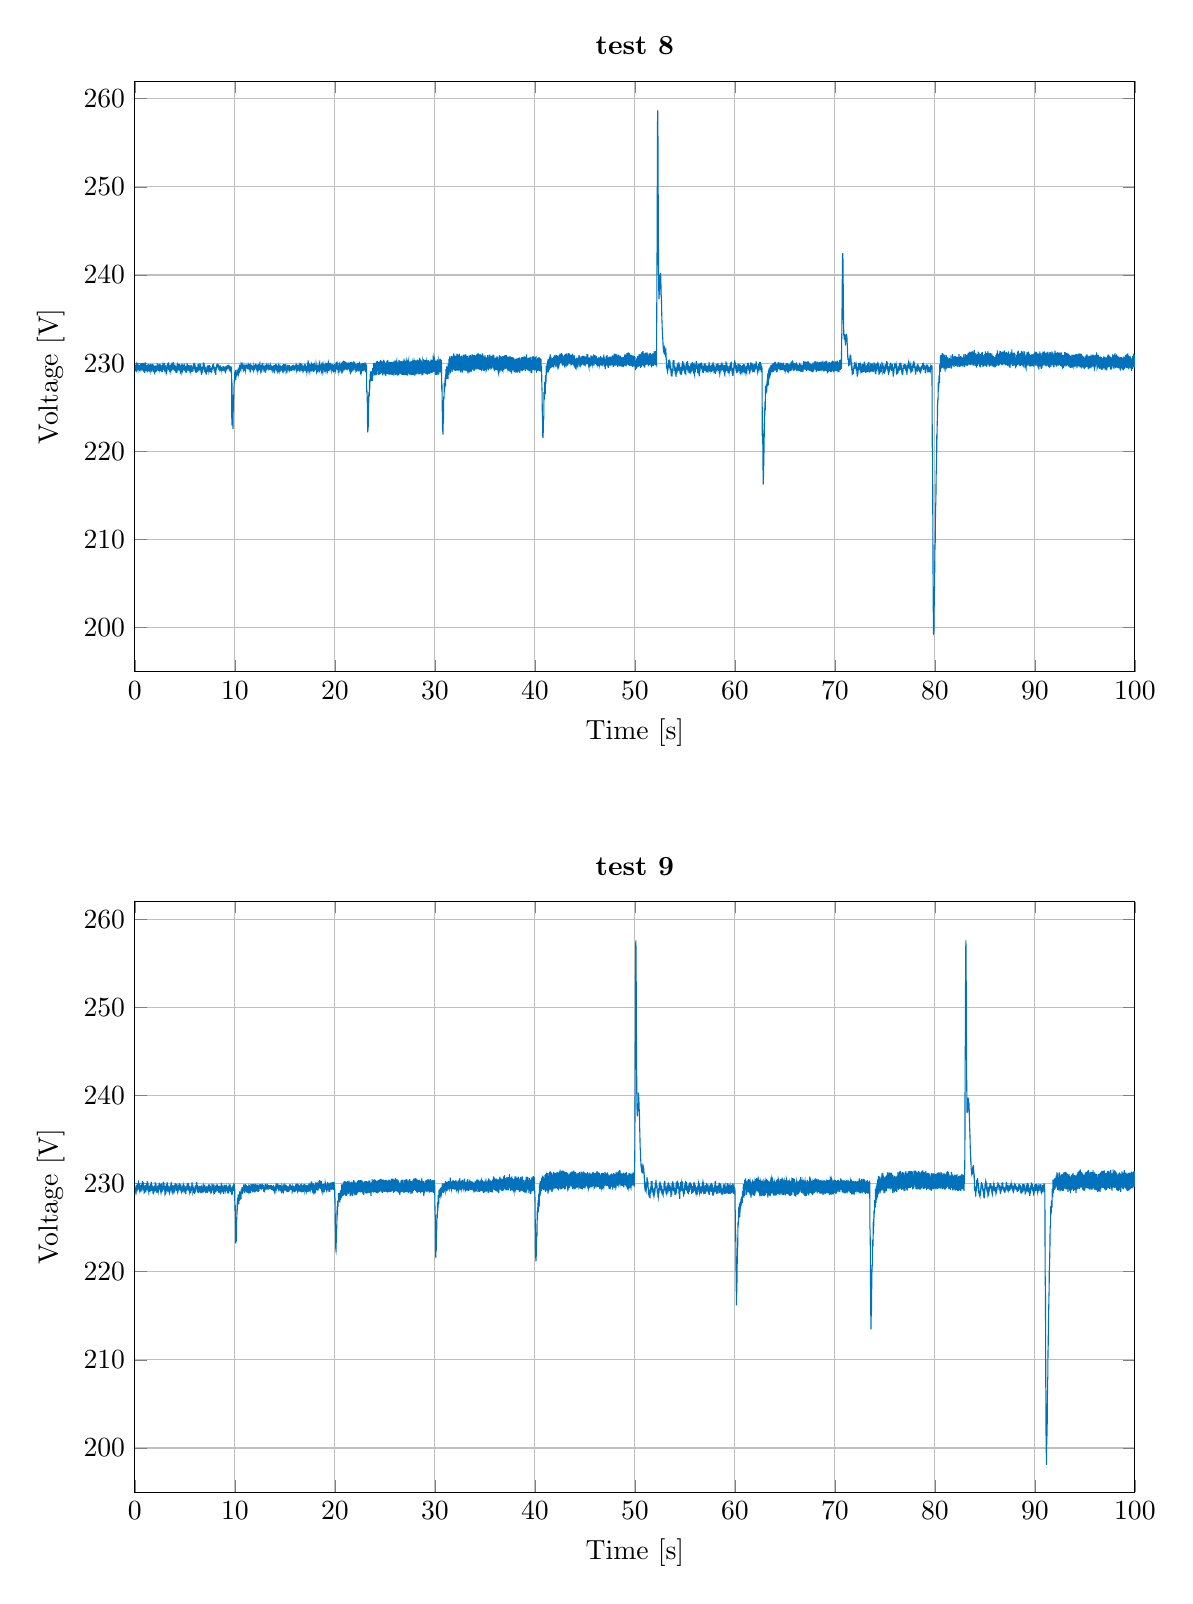
\begin{tikzpicture}

\begin{axis}[%
width=5in,
height=2.953in,
at={(1.142in,5.054in)},
scale only axis,
xmin=0,
xmax=100,
xlabel={Time [s]},
ymajorgrids,
xmajorgrids,
ymin=195,
ymax=262,
ylabel={Voltage [V]},
axis background/.style={fill=white},
title style={font=\bfseries},
title={test 8}
]
\addplot [color=mycolor1,solid,forget plot]
  table[row sep=crcr]{%
0.016	229.064427655595\\
0.032	229.268992563583\\
0.048	229.200886990589\\
0.064	229.186170117703\\
0.08	229.841385961772\\
0.096	229.230004252802\\
0.112	229.446623614044\\
0.128	229.472701103133\\
0.144	229.38574115055\\
0.16	230.049999474053\\
0.176	229.332871976809\\
0.192	229.607088494542\\
0.208	229.475571411335\\
0.224	229.412792198357\\
0.24	230.029175437358\\
0.256	229.406538046104\\
0.272	229.536019802206\\
0.288	229.457833236643\\
0.304	229.320947226006\\
0.32	229.942528182233\\
0.336	229.283078054249\\
0.352	229.452813096162\\
0.368	229.379819565047\\
0.384	229.305551020167\\
0.4	229.791578503032\\
0.416	229.235740715538\\
0.432	229.296078584379\\
0.448	229.301161273303\\
0.464	229.274147703777\\
0.48	229.812952606634\\
0.496	229.144430953118\\
0.512	229.327891644817\\
0.528	229.266448814618\\
0.544	229.379769137625\\
0.56	229.925353828985\\
0.576	229.289177919983\\
0.592	229.483070241715\\
0.608	229.487774000021\\
0.624	229.433263672927\\
0.64	229.976058149762\\
0.656	229.253745134704\\
0.672	229.471452893126\\
0.688	229.416554970101\\
0.704	229.38824469363\\
0.72	229.932055519867\\
0.736	229.308868483167\\
0.752	229.48240563656\\
0.768	229.486837287086\\
0.784	229.407664805459\\
0.8	230.027789970771\\
0.816	229.372401228744\\
0.832	229.584889649888\\
0.848	229.489088541718\\
0.864	229.541522605604\\
0.88	230.046507453993\\
0.896	229.310924074602\\
0.912	229.34702065724\\
0.928	229.141345681057\\
0.944	228.995970913945\\
0.96	229.588988228108\\
0.976	228.909763228592\\
0.992	229.215660906661\\
1.008	229.298135833643\\
1.024	229.4197809169\\
1.04	230.104092357186\\
1.056	229.478568649218\\
1.072	229.626366075717\\
1.088	229.555188675072\\
1.104	229.304307937754\\
1.12	229.796268454199\\
1.136	229.06428619795\\
1.152	229.326496594784\\
1.168	229.26484103821\\
1.184	229.231667674679\\
1.2	229.790473072533\\
1.216	229.07788720938\\
1.232	229.286121615709\\
1.248	229.296738048819\\
1.264	229.238628615591\\
1.28	229.847095359705\\
1.296	229.111592249107\\
1.312	229.42007250242\\
1.328	229.351910470775\\
1.344	229.313566543391\\
1.36	229.923125622851\\
1.376	229.259114881277\\
1.392	229.438856306793\\
1.408	229.416015767817\\
1.424	229.302411307644\\
1.44	229.842011365517\\
1.456	229.104413650349\\
1.472	229.299754670142\\
1.488	229.166366004794\\
1.504	229.098751495271\\
1.52	229.697441565087\\
1.536	229.269326464527\\
1.552	229.516365966359\\
1.568	229.448735382719\\
1.584	229.368082443392\\
1.6	229.911869669167\\
1.616	229.146879944844\\
1.632	229.429133576289\\
1.648	229.374372638137\\
1.664	229.260295620547\\
1.68	229.817961372184\\
1.696	229.037519762624\\
1.712	229.276177010435\\
1.728	229.305895328691\\
1.744	229.191752995775\\
1.76	229.890090318109\\
1.776	229.188370977064\\
1.792	229.418356073531\\
1.808	229.280984571422\\
1.824	229.240524941216\\
1.84	229.844348808725\\
1.856	229.186988006938\\
1.872	229.322251369125\\
1.888	229.259745439836\\
1.904	229.177261384152\\
1.92	229.712164555557\\
1.936	228.997691202164\\
1.952	229.227358834196\\
1.968	229.11807531442\\
1.984	229.059572384378\\
2	229.693437722317\\
2.016	229.1339271031\\
2.032	229.443709648304\\
2.048	229.468714533518\\
2.064	229.203630023444\\
2.08	229.762586525112\\
2.096	228.969824989802\\
2.112	229.305476589894\\
2.128	229.273743217598\\
2.144	229.138070735502\\
2.16	229.67421867951\\
2.176	229.074386009092\\
2.192	229.461410140927\\
2.208	229.502460982403\\
2.224	229.387015834455\\
2.24	229.977097258963\\
2.256	229.280125285415\\
2.272	229.647483232962\\
2.288	229.520553728726\\
2.304	229.329649387974\\
2.32	229.867736428206\\
2.336	229.090273758978\\
2.352	229.356760550568\\
2.368	229.326754645978\\
2.384	229.180976743819\\
2.4	229.804584329657\\
2.416	229.088203325551\\
2.432	229.483340855259\\
2.448	229.422115406266\\
2.464	229.332748803986\\
2.48	229.94975774933\\
2.496	229.239291447515\\
2.512	229.452421971485\\
2.528	229.463463003037\\
2.544	229.343779617582\\
2.56	229.87706874785\\
2.576	229.129357249424\\
2.592	229.485826955706\\
2.608	229.447304396066\\
2.624	229.309054480792\\
2.64	229.750382787535\\
2.656	229.011802106961\\
2.672	229.258123351292\\
2.688	229.216631488512\\
2.704	229.039890849123\\
2.72	229.707421308946\\
2.736	228.986192983928\\
2.752	229.36115015887\\
2.768	229.419396859991\\
2.784	229.411006082004\\
2.8	230.023119931966\\
2.816	229.369681827834\\
2.832	229.674013085734\\
2.848	229.564462456677\\
2.864	229.285794962907\\
2.88	229.923992874292\\
2.896	229.207737203383\\
2.912	229.546636062593\\
2.928	229.531091969805\\
2.944	229.430346359641\\
2.96	230.001630072266\\
2.976	229.320417613643\\
2.992	229.494742106281\\
3.008	229.346227829263\\
3.024	229.1435236893\\
3.04	229.743696815765\\
3.056	229.020467259944\\
3.072	229.241136934574\\
3.088	229.155121294884\\
3.104	229.064333392062\\
3.12	229.557200140512\\
3.136	228.798992839063\\
3.152	229.090214613431\\
3.168	229.236815813733\\
3.184	229.164479250309\\
3.2	229.806376471517\\
3.216	229.078642298574\\
3.232	229.463036957679\\
3.248	229.485707357013\\
3.264	229.351013917212\\
3.28	229.974043990031\\
3.296	229.336200224898\\
3.312	229.655733275619\\
3.328	229.659772600434\\
3.344	229.506579944012\\
3.36	230.084639293135\\
3.376	229.230552839906\\
3.392	229.435479615159\\
3.408	229.275643220109\\
3.424	229.23433822935\\
3.44	229.8461519995\\
3.456	229.16640888968\\
3.472	229.383074693003\\
3.488	229.335824207081\\
3.504	229.237282371725\\
3.52	229.764099916261\\
3.536	229.074684655995\\
3.552	229.350543045979\\
3.568	229.240121357751\\
3.584	229.188982925782\\
3.6	229.717444862678\\
3.616	229.106144168299\\
3.632	229.404342383352\\
3.648	229.569118356455\\
3.664	229.41863187076\\
3.68	229.883210027551\\
3.696	229.17118746773\\
3.712	229.578273245292\\
3.728	229.526591325951\\
3.744	229.498541818714\\
3.76	229.989608253154\\
3.776	229.415116016426\\
3.792	229.811072313502\\
3.808	229.78035336516\\
3.824	229.686940162664\\
3.84	230.147012434497\\
3.856	229.272503724728\\
3.872	229.565782355264\\
3.888	229.493931919431\\
3.904	229.277955070592\\
3.92	229.839054375423\\
3.936	229.185490867854\\
3.952	229.382476073471\\
3.968	229.316620667495\\
3.984	229.199344430631\\
4	229.845089626701\\
4.016	229.108154544852\\
4.032	229.337306316279\\
4.048	229.21909981101\\
4.064	229.175028145282\\
4.08	229.72765916127\\
4.096	228.94346715271\\
4.112	229.141698252073\\
4.128	229.086592205384\\
4.144	228.891096702992\\
4.16	229.539589773474\\
4.176	228.927567107321\\
4.192	229.444459351568\\
4.208	229.415874355435\\
4.224	229.350912764681\\
4.24	229.947605465271\\
4.256	229.371683891881\\
4.272	229.770080459263\\
4.288	229.705471128722\\
4.304	229.529514791928\\
4.32	229.876134005518\\
4.336	229.174397015554\\
4.352	229.439492343087\\
4.368	229.352709776683\\
4.384	229.379969107527\\
4.4	229.943145384196\\
4.416	229.299381150698\\
4.432	229.464603295204\\
4.448	229.386389081574\\
4.464	229.247657679501\\
4.48	229.849159103118\\
4.496	229.071281893723\\
4.512	229.351208616023\\
4.528	229.234377021463\\
4.544	229.143666117659\\
4.56	229.697238205908\\
4.576	228.947402732576\\
4.592	229.285855438678\\
4.608	229.234778464806\\
4.624	229.143293474419\\
4.64	229.835840746861\\
4.656	229.186683241919\\
4.672	229.521609009181\\
4.688	229.442610644395\\
4.704	229.352689572463\\
4.72	229.79118712959\\
4.736	229.208012769987\\
4.752	229.527315749968\\
4.768	229.439730276759\\
4.784	229.350721563552\\
4.8	229.87386275335\\
4.816	229.297094961862\\
4.832	229.740189034963\\
4.848	229.591404442217\\
4.864	229.32221974023\\
4.88	229.77987520829\\
4.896	229.197265144314\\
4.912	229.567711118273\\
4.928	229.539019112472\\
4.944	229.385152787029\\
4.96	229.928765439307\\
4.976	229.147902073855\\
4.992	229.423365306433\\
5.008	229.301524502981\\
5.024	229.0912153979\\
5.04	229.656625169261\\
5.056	228.959832173375\\
5.072	229.341384231898\\
5.088	229.300098583624\\
5.104	229.080473717489\\
5.12	229.560624461295\\
5.136	228.922175675451\\
5.152	229.411539138412\\
5.168	229.446923385499\\
5.184	229.354972880064\\
5.2	229.842770908417\\
5.216	229.256561896778\\
5.232	229.684754975306\\
5.248	229.607353725382\\
5.264	229.386819909145\\
5.28	229.760391307605\\
5.296	229.165905668138\\
5.312	229.442399493084\\
5.328	229.335719540336\\
5.344	229.300470449942\\
5.36	229.786375650945\\
5.376	229.219661154471\\
5.392	229.584776492977\\
5.408	229.545116706476\\
5.424	229.371665293611\\
5.44	229.745616738851\\
5.456	229.096096702613\\
5.472	229.458841669808\\
5.488	229.243268805715\\
5.504	228.993927295684\\
5.52	229.582970303046\\
5.536	228.908602412743\\
5.552	229.239852084743\\
5.568	229.155896856753\\
5.584	229.062693287762\\
5.6	229.794197694347\\
5.616	229.156931530704\\
5.632	229.557123404506\\
5.648	229.419134828248\\
5.664	229.234734510544\\
5.68	229.668502486651\\
5.696	229.009267764456\\
5.712	229.390051734771\\
5.728	229.322540374843\\
5.744	229.192626701306\\
5.76	229.570614778756\\
5.776	229.033669134698\\
5.792	229.492153053831\\
5.808	229.365689612917\\
5.824	229.328715917087\\
5.84	229.814418271884\\
5.856	229.428743437498\\
5.872	229.889051932059\\
5.888	229.774677063228\\
5.904	229.740741964928\\
5.92	230.047294801451\\
5.936	229.342619051404\\
5.952	229.667632936269\\
5.968	229.459548337818\\
5.984	229.392508465476\\
6	229.94526748273\\
6.016	229.190347117459\\
6.032	229.458535575629\\
6.048	229.399532121354\\
6.064	229.232067747244\\
6.08	229.713029649796\\
6.096	228.966892600863\\
6.112	229.270592925351\\
6.128	229.180626589129\\
6.144	228.917674742062\\
6.16	229.480153017486\\
6.176	228.996271035131\\
6.192	229.422924539713\\
6.208	229.286280050125\\
6.224	229.127397307656\\
6.24	229.563171412504\\
6.256	228.97883786168\\
6.272	229.441208327697\\
6.288	229.454032066099\\
6.304	229.485534547499\\
6.32	229.895543572315\\
6.336	229.354954113106\\
6.352	229.688996773316\\
6.368	229.52221438675\\
6.384	229.436114856138\\
6.4	229.801375797199\\
6.416	229.194378707467\\
6.432	229.540761683888\\
6.448	229.454640135741\\
6.464	229.306593072637\\
6.48	229.743678145171\\
6.496	229.187359617138\\
6.512	229.555473192726\\
6.528	229.464037744485\\
6.544	229.445120582738\\
6.56	229.952918653365\\
6.576	229.257182711305\\
6.592	229.473174129013\\
6.608	229.150610558354\\
6.624	228.916583934022\\
6.64	229.32623410883\\
6.656	228.689681763651\\
6.672	229.234960008348\\
6.688	229.261846230261\\
6.704	229.205903684475\\
6.72	229.60867777027\\
6.736	229.027526881539\\
6.752	229.463283446909\\
6.768	229.304933448574\\
6.784	229.232902375633\\
6.8	229.641221453795\\
6.816	229.222044042396\\
6.832	229.657516374666\\
6.848	229.580201443819\\
6.864	229.644933041904\\
6.88	230.10120100302\\
6.896	229.602165714518\\
6.912	229.970825992309\\
6.928	229.636856550933\\
6.944	229.375313675663\\
6.96	229.729793251697\\
6.976	229.018243826426\\
6.992	229.347957829565\\
7.008	229.23137167407\\
7.024	229.067581451552\\
7.04	229.563535397593\\
7.056	228.883194630574\\
7.072	229.246709653438\\
7.088	229.101717416914\\
7.104	228.931308626287\\
7.12	229.296991250605\\
7.136	228.695444224666\\
7.152	229.086325707182\\
7.168	229.062099001779\\
7.184	229.051588430937\\
7.2	229.551365151024\\
7.216	229.232967665545\\
7.232	229.664847182513\\
7.248	229.452791819712\\
7.264	229.379000198049\\
7.28	229.732783821998\\
7.296	229.331990349059\\
7.312	229.73842808398\\
7.328	229.394485205905\\
7.344	229.265990614332\\
7.36	229.55440539639\\
7.376	229.127366610731\\
7.392	229.601315962859\\
7.408	229.474388516231\\
7.424	229.372091451947\\
7.44	229.777882035668\\
7.456	229.238480159337\\
7.472	229.564302383041\\
7.488	229.38640112434\\
7.504	229.266887732554\\
7.52	229.650705981375\\
7.536	229.007936152844\\
7.552	229.41166197508\\
7.568	229.285704140466\\
7.584	229.134573411268\\
7.6	229.447947284895\\
7.616	228.967851465346\\
7.632	229.38190952986\\
7.648	229.187226666622\\
7.664	229.122235576255\\
7.68	229.451203153207\\
7.696	229.056869488589\\
7.712	229.585192688382\\
7.728	229.383644023313\\
7.744	229.374775413933\\
7.76	229.593521223451\\
7.776	229.324735051008\\
7.792	229.830602600388\\
7.808	229.626765505407\\
7.824	229.640006240118\\
7.84	229.95849188002\\
7.856	229.564113216433\\
7.872	229.835141447604\\
7.888	229.577689709799\\
7.904	229.400018182566\\
7.92	229.633855481169\\
7.936	229.095911014751\\
7.952	229.464032133166\\
7.968	229.283114917035\\
7.984	229.208040522275\\
8	229.513744834145\\
8.016	228.900656563765\\
8.032	229.279624145659\\
8.048	229.081441387915\\
8.064	228.904879920009\\
8.08	229.124942195694\\
8.096	228.669087387695\\
8.112	229.298905706788\\
8.128	229.262748089459\\
8.144	229.333917841673\\
8.16	229.702259190522\\
8.176	229.33390587737\\
8.192	229.821824545826\\
8.208	229.664993874368\\
8.224	229.706312610552\\
8.24	229.930224078385\\
8.256	229.636677926694\\
8.272	229.944945328503\\
8.288	229.647435230488\\
8.304	229.642911955852\\
8.32	229.804934522768\\
8.336	229.463741837706\\
8.352	229.854596940071\\
8.368	229.485971639765\\
8.384	229.323062944073\\
8.4	229.63508886211\\
8.416	229.229892158922\\
8.432	229.604185113324\\
8.448	229.392263022183\\
8.464	229.327400981701\\
8.48	229.728193747875\\
8.496	229.149698598966\\
8.512	229.49968498515\\
8.528	229.30571750782\\
8.544	229.184181435447\\
8.56	229.736610963314\\
8.576	229.215530733814\\
8.592	229.572150603428\\
8.608	229.398504661232\\
8.624	229.268854718724\\
8.64	229.560367691362\\
8.656	229.105493701278\\
8.672	229.5317557452\\
8.688	229.27914938689\\
8.704	229.120129391208\\
8.72	229.47134056995\\
8.736	229.111576911684\\
8.752	229.533916321481\\
8.768	229.305713186958\\
8.784	229.292747150921\\
8.8	229.64067665739\\
8.816	229.245573444196\\
8.832	229.651073276237\\
8.848	229.413934473195\\
8.864	229.182271094187\\
8.88	229.545190997241\\
8.896	229.097129337999\\
8.912	229.484743032199\\
8.928	229.323106704037\\
8.944	229.206918033804\\
8.96	229.608650028152\\
8.976	229.080863365453\\
8.992	229.438996476506\\
9.008	229.232692707784\\
9.024	229.077455090573\\
9.04	229.388349957731\\
9.056	228.849963887813\\
9.072	229.329103353785\\
9.088	229.291756820116\\
9.104	229.356279551998\\
9.12	229.65797994039\\
9.136	229.208854110434\\
9.152	229.680896994914\\
9.168	229.472913309757\\
9.184	229.410630632502\\
9.2	229.690715335454\\
9.216	229.32701959224\\
9.232	229.738831127096\\
9.248	229.531921207839\\
9.264	229.499778977419\\
9.28	229.748666228288\\
9.296	229.402335901126\\
9.312	229.778648637495\\
9.328	229.552587262574\\
9.344	229.520188995313\\
9.36	229.844554733724\\
9.376	229.451218952181\\
9.392	229.745264506417\\
9.408	229.376655402668\\
9.424	229.338926191208\\
9.44	229.714703147942\\
9.456	229.259034065655\\
9.472	229.633664557694\\
9.488	229.410466278477\\
9.504	229.320376277629\\
9.52	229.656627794122\\
9.536	229.047379988031\\
9.552	229.413341060431\\
9.568	229.215095147076\\
9.584	229.193362053371\\
9.6	229.617002774202\\
9.616	229.197764611183\\
9.632	229.596344664625\\
9.648	229.475804245851\\
9.664	229.391211353035\\
9.68	229.605324675344\\
9.696	222.947772817164\\
9.712	227.724009479168\\
9.728	226.688114047742\\
9.744	225.788274293474\\
9.76	225.22795799241\\
9.776	224.538086593297\\
9.792	223.631745354665\\
9.808	222.519419171351\\
9.824	224.288439164994\\
9.84	224.570635868611\\
9.856	224.601547790095\\
9.872	225.719076936514\\
9.888	225.950982357793\\
9.904	227.273086249086\\
9.92	227.358468008874\\
9.936	228.05377214986\\
9.952	227.869386718192\\
9.968	227.983388011283\\
9.984	228.971409444748\\
10	228.466537252619\\
10.016	228.421633478975\\
10.032	228.405105547057\\
10.048	229.221100314441\\
10.064	228.760825869602\\
10.08	228.532696847045\\
10.096	228.090022424992\\
10.112	228.463376899668\\
10.128	229.018342404364\\
10.144	228.759899013698\\
10.16	228.509443801909\\
10.176	228.725843657976\\
10.192	228.834304108031\\
10.208	229.257753846356\\
10.224	229.063706554168\\
10.24	228.643485490637\\
10.256	228.841323528064\\
10.272	229.04374567414\\
10.288	229.192320686901\\
10.304	228.895262954532\\
10.32	228.794609741371\\
10.336	229.111513022069\\
10.352	229.034101520775\\
10.368	229.420721670777\\
10.384	228.766136598018\\
10.4	229.275727071853\\
10.416	229.164062383815\\
10.432	229.028226167243\\
10.448	229.628097612003\\
10.464	228.915640051849\\
10.48	229.614763071499\\
10.496	229.582950272004\\
10.512	229.370278682605\\
10.528	229.834532589427\\
10.544	229.354844610515\\
10.56	229.711731772298\\
10.576	229.39070999571\\
10.592	229.449556565817\\
10.608	229.662014487451\\
10.624	229.530935945904\\
10.64	229.755691703703\\
10.656	229.424708576421\\
10.672	229.437684006142\\
10.688	229.686379524498\\
10.704	229.712631146526\\
10.72	230.079258905402\\
10.736	229.672015641485\\
10.752	229.696901553342\\
10.768	229.645777435992\\
10.784	229.560341540848\\
10.8	229.859435328326\\
10.816	229.55989778995\\
10.832	229.512689965262\\
10.848	229.698840715079\\
10.864	229.371954240125\\
10.88	229.654924984385\\
10.896	229.2947825531\\
10.912	229.356347948928\\
10.928	229.577444423169\\
10.944	229.442725901894\\
10.96	229.813756351569\\
10.976	229.569979919468\\
10.992	229.408801163032\\
11.008	229.447101175542\\
11.024	229.145527089646\\
11.04	229.443546184263\\
11.056	229.1574752057\\
11.072	229.258036890033\\
11.088	229.497220705871\\
11.104	229.483568806696\\
11.12	229.859586306746\\
11.136	229.506542493657\\
11.152	229.513041286626\\
11.168	229.720058906553\\
11.184	229.533129909852\\
11.2	229.829820100242\\
11.216	229.403163795558\\
11.232	229.548606841975\\
11.248	229.65709065265\\
11.264	229.604812583615\\
11.28	229.753778675755\\
11.296	229.291097744418\\
11.312	229.422488199705\\
11.328	229.610765164278\\
11.344	229.472493171246\\
11.36	229.737158830792\\
11.376	229.303233686802\\
11.392	229.498380954304\\
11.408	229.655063746236\\
11.424	229.66626063156\\
11.44	229.929589063192\\
11.456	229.477204685177\\
11.472	229.375856823907\\
11.488	229.510764814287\\
11.504	229.399636110155\\
11.52	229.724659854149\\
11.536	229.36654440335\\
11.552	229.418751891406\\
11.568	229.593564382283\\
11.584	229.479247883539\\
11.6	229.672368530792\\
11.616	229.394789176272\\
11.632	229.479205056294\\
11.648	229.840953335016\\
11.664	229.563198514071\\
11.68	229.812745090211\\
11.696	229.430460460626\\
11.712	229.396725970643\\
11.728	229.585344875221\\
11.744	229.401700821865\\
11.76	229.617640357257\\
11.776	229.265020988468\\
11.792	229.270818667958\\
11.808	229.582649410633\\
11.824	229.45089423014\\
11.84	229.72020646208\\
11.856	229.362384553258\\
11.872	229.471336209228\\
11.888	229.650714537396\\
11.904	229.509221295579\\
11.92	229.69290343948\\
11.936	229.314183112596\\
11.952	229.320373841297\\
11.968	229.536516482596\\
11.984	229.479130970876\\
12	229.795501798809\\
12.016	229.338918767167\\
12.032	229.522175622486\\
12.048	229.657943170422\\
12.064	229.679382936229\\
12.08	229.943205077002\\
12.096	229.559027126838\\
12.112	229.589907613865\\
12.128	229.635281790919\\
12.144	229.547549234745\\
12.16	229.841144516788\\
12.176	229.26410711835\\
12.192	229.373279077127\\
12.208	229.462163285366\\
12.224	229.365530558835\\
12.24	229.587397029621\\
12.256	229.21256003735\\
12.272	229.328949592192\\
12.288	229.546184469914\\
12.304	229.484713177742\\
12.32	229.81739438526\\
12.336	229.388660010418\\
12.352	229.565362074789\\
12.368	229.721229447935\\
12.384	229.717749408731\\
12.4	229.914681683179\\
12.416	229.503632974924\\
12.432	229.594635097423\\
12.448	229.733155829848\\
12.464	229.565457776844\\
12.48	229.780237683196\\
12.496	229.281558857126\\
12.512	229.266574421158\\
12.528	229.428625907684\\
12.544	229.417366369585\\
12.56	229.645296389353\\
12.576	229.259356906071\\
12.592	229.374042277722\\
12.608	229.644855405841\\
12.624	229.528479157966\\
12.64	229.827520969543\\
12.656	229.38605488548\\
12.672	229.488379505456\\
12.688	229.550806371644\\
12.704	229.485290782731\\
12.72	229.703229722902\\
12.736	229.341520895567\\
12.752	229.419572997273\\
12.768	229.77922017273\\
12.784	229.806649988293\\
12.8	230.04172866853\\
12.816	229.566569373997\\
12.832	229.567797985895\\
12.848	229.498948495748\\
12.864	229.412736601276\\
12.88	229.655872020853\\
12.896	229.323234632462\\
12.912	229.356024442031\\
12.928	229.588794185134\\
12.944	229.418525179485\\
12.96	229.688609997748\\
12.976	229.286553835239\\
12.992	229.342457000299\\
13.008	229.504339406468\\
13.024	229.399862346196\\
13.04	229.59803677247\\
13.056	229.2340810874\\
13.072	229.176965664918\\
13.088	229.424194323219\\
13.104	229.407892570879\\
13.12	229.819331186574\\
13.136	229.409399720435\\
13.152	229.554398503198\\
13.168	229.677041593998\\
13.184	229.567572203653\\
13.2	229.738200806105\\
13.216	229.33390756904\\
13.232	229.332200613581\\
13.248	229.47623823984\\
13.264	229.341547434551\\
13.28	229.713018871674\\
13.296	229.369597028075\\
13.312	229.494679977371\\
13.328	229.643951658667\\
13.344	229.553707175047\\
13.36	229.754468920664\\
13.376	229.32566618179\\
13.392	229.447109261994\\
13.408	229.550128371837\\
13.424	229.403814636556\\
13.44	229.714113230977\\
13.456	229.217872384689\\
13.472	229.488518162302\\
13.488	229.515602320612\\
13.504	229.581773705065\\
13.52	229.822447442449\\
13.536	229.405488901679\\
13.552	229.581002816517\\
13.568	229.679910922131\\
13.584	229.442050160906\\
13.6	229.72868148717\\
13.616	229.248337156256\\
13.632	229.40981248917\\
13.648	229.541634689195\\
13.664	229.525028447761\\
13.68	229.753005038916\\
13.696	229.285795274663\\
13.712	229.205639701436\\
13.728	229.392727707142\\
13.744	229.370748351914\\
13.76	229.675706144266\\
13.776	229.213019937314\\
13.792	229.350446549647\\
13.808	229.505814420353\\
13.824	229.488066611932\\
13.84	229.688468250866\\
13.856	229.278916482042\\
13.872	229.35890900276\\
13.888	229.491927588225\\
13.904	229.403175924969\\
13.92	229.772185984114\\
13.936	229.284920742371\\
13.952	229.414166410609\\
13.968	229.511170121651\\
13.984	229.51856825301\\
14	229.775788442974\\
14.016	229.360360930855\\
14.032	229.470606319556\\
14.048	229.658044372697\\
14.064	229.611894241221\\
14.08	229.907739085564\\
14.096	229.45952135007\\
14.112	229.503591453493\\
14.128	229.583817781762\\
14.144	229.565090426878\\
14.16	229.762009012863\\
14.176	229.372349419061\\
14.192	229.420333100438\\
14.208	229.566736163267\\
14.224	229.449647518623\\
14.24	229.699506071768\\
14.256	229.250260981703\\
14.272	229.339248063721\\
14.288	229.480620636834\\
14.304	229.485229866626\\
14.32	229.711546217971\\
14.336	229.32705434973\\
14.352	229.425986552671\\
14.368	229.6042982859\\
14.384	229.476345236679\\
14.4	229.751775212175\\
14.416	229.30137169114\\
14.432	229.430418052354\\
14.448	229.559216475421\\
14.464	229.493258224456\\
14.48	229.688639935051\\
14.496	229.268514433968\\
14.512	229.36955776355\\
14.528	229.565036674425\\
14.544	229.46824623405\\
14.56	229.731005526493\\
14.576	229.166523580414\\
14.592	229.345091799542\\
14.608	229.420498197953\\
14.624	229.425532350674\\
14.64	229.68239422444\\
14.656	229.24635438798\\
14.672	229.248315642051\\
14.688	229.393583967491\\
14.704	229.329546723581\\
14.72	229.636696283645\\
14.736	229.194015315582\\
14.752	229.44514014659\\
14.768	229.608478569125\\
14.784	229.57314243202\\
14.8	229.773655014747\\
14.816	229.373554127799\\
14.832	229.465066942759\\
14.848	229.671655940556\\
14.864	229.651424133997\\
14.88	229.923881554365\\
14.896	229.393262256557\\
14.912	229.499677158266\\
14.928	229.562268806499\\
14.944	229.44637615355\\
14.96	229.656636751516\\
14.976	229.161567623648\\
14.992	229.308973282657\\
15.008	229.50140384355\\
15.024	229.455385729137\\
15.04	229.87707007031\\
15.056	229.325694729425\\
15.072	229.503752405583\\
15.088	229.572497061006\\
15.104	229.594831983071\\
15.12	229.824548639786\\
15.136	229.117744193272\\
15.152	229.20271914894\\
15.168	229.325788040516\\
15.184	229.249511448441\\
15.2	229.541117143257\\
15.216	228.944590398317\\
15.232	229.167674323654\\
15.248	229.272639128129\\
15.264	229.461061544632\\
15.28	229.810399924265\\
15.296	229.211295258662\\
15.312	229.366179384734\\
15.328	229.559298584848\\
15.344	229.508321641058\\
15.36	229.775955708277\\
15.376	229.166139191115\\
15.392	229.395989253236\\
15.408	229.521357123303\\
15.424	229.516836874544\\
15.44	229.782658274832\\
15.456	229.180149509075\\
15.472	229.227653875675\\
15.488	229.376978686189\\
15.504	229.359519139049\\
15.52	229.659305809841\\
15.536	229.147567818242\\
15.552	229.30553032737\\
15.568	229.390504597791\\
15.584	229.380610712188\\
15.6	229.616418006046\\
15.616	229.135695081816\\
15.632	229.26688490523\\
15.648	229.413053573755\\
15.664	229.386055528849\\
15.68	229.678600609246\\
15.696	229.111768663695\\
15.712	229.308999504352\\
15.728	229.426438657973\\
15.744	229.52281353114\\
15.76	229.771149450573\\
15.776	229.276921601024\\
15.792	229.395582681562\\
15.808	229.54088225887\\
15.824	229.489194490043\\
15.84	229.794391884371\\
15.856	229.212319881464\\
15.872	229.382805260206\\
15.888	229.492245451779\\
15.904	229.485094068408\\
15.92	229.703906668972\\
15.936	229.158905074434\\
15.952	229.340437877026\\
15.968	229.468671483312\\
15.984	229.47577311125\\
16	229.747764917413\\
16.016	229.202097671063\\
16.032	229.447264379146\\
16.048	229.639833167079\\
16.064	229.624378103627\\
16.08	229.829526216775\\
16.096	229.36931189007\\
16.112	229.606640930366\\
16.128	229.743937728405\\
16.144	229.648852360133\\
16.16	229.92796591696\\
16.176	229.238689146222\\
16.192	229.309776541767\\
16.208	229.42883895079\\
16.224	229.470559081125\\
16.24	229.693869956391\\
16.256	229.084853015457\\
16.272	229.237680824828\\
16.288	229.445213069737\\
16.304	229.415632878551\\
16.32	229.809394040461\\
16.336	229.261412900115\\
16.352	229.512352274408\\
16.368	229.639228542252\\
16.384	229.626057641209\\
16.4	229.825322342351\\
16.416	229.150644472529\\
16.432	229.306420332347\\
16.448	229.523981907933\\
16.464	229.390424667206\\
16.48	229.681839712937\\
16.496	229.018117399985\\
16.512	229.229134862539\\
16.528	229.649489726587\\
16.544	229.74773176454\\
16.56	230.017445314501\\
16.576	229.411575708936\\
16.592	229.528238515668\\
16.608	229.740061352485\\
16.624	229.719689796953\\
16.64	229.920021624182\\
16.656	229.16098350016\\
16.672	229.343803515092\\
16.688	229.580397312564\\
16.704	229.572140583894\\
16.72	229.780402093034\\
16.736	229.132841649702\\
16.752	229.280316104305\\
16.768	229.476349896087\\
16.784	229.362945515121\\
16.8	229.647307062151\\
16.816	228.946570524169\\
16.832	229.128245077703\\
16.848	229.374757900179\\
16.864	229.467846181672\\
16.88	229.732550163718\\
16.896	229.072708860277\\
16.912	229.30312026311\\
16.928	229.629433145539\\
16.944	229.628920365875\\
16.96	229.89737616652\\
16.976	229.219416863\\
16.992	229.415514861949\\
17.008	229.637972795358\\
17.024	229.604073335165\\
17.04	229.76287789842\\
17.056	229.120991875563\\
17.072	229.255667651726\\
17.088	229.495425997032\\
17.104	229.406337292685\\
17.12	229.645176231842\\
17.136	228.926703281165\\
17.152	229.121926226774\\
17.168	229.422427618031\\
17.184	229.479904580017\\
17.2	229.695640052398\\
17.216	229.024508501292\\
17.232	229.123335020614\\
17.248	229.623613629181\\
17.264	229.53070641334\\
17.28	229.730509646627\\
17.296	229.12338554379\\
17.312	229.264904396214\\
17.328	229.810525668865\\
17.344	229.707968396289\\
17.36	229.808686830622\\
17.376	229.243007357199\\
17.392	229.145712076619\\
17.408	229.539766185013\\
17.424	229.299220741722\\
17.44	229.524575493104\\
17.456	229.081414268917\\
17.472	229.227603005656\\
17.488	229.718306435054\\
17.504	229.660731129491\\
17.52	229.858188951339\\
17.536	229.250121788062\\
17.552	229.350486443651\\
17.568	229.687433903611\\
17.584	229.514848787569\\
17.6	229.737776928869\\
17.616	229.098047751783\\
17.632	229.264754525069\\
17.648	229.641279330117\\
17.664	229.551458600189\\
17.68	229.682871930177\\
17.696	229.045322458249\\
17.712	229.21701365979\\
17.728	229.71999164492\\
17.744	229.645075711799\\
17.76	229.890068456541\\
17.776	229.24380826771\\
17.792	229.241078345201\\
17.808	229.69435112335\\
17.824	229.509136477359\\
17.84	229.587842059346\\
17.856	229.031154016096\\
17.872	229.217044117579\\
17.888	229.971463897572\\
17.904	229.813097234189\\
17.92	229.93111902249\\
17.936	229.357253690559\\
17.952	229.426175568343\\
17.968	229.899023493452\\
17.984	229.75064863216\\
18	229.848632516908\\
18.016	229.298991802523\\
18.032	229.334086034727\\
18.048	229.828895340918\\
18.064	229.69659790269\\
18.08	229.84159370696\\
18.096	229.202181938104\\
18.112	229.312672945269\\
18.128	229.711382611653\\
18.144	229.565206654831\\
18.16	229.696082851384\\
18.176	229.104746723361\\
18.192	229.176471482389\\
18.208	229.694636257702\\
18.224	229.58714772377\\
18.24	229.756465903559\\
18.256	229.074494676953\\
18.272	229.10518307263\\
18.288	229.663755705628\\
18.304	229.552453080423\\
18.32	229.666997807276\\
18.336	229.101446981142\\
18.352	229.219210648734\\
18.368	229.828094635179\\
18.384	229.664509446345\\
18.4	229.793195912753\\
18.416	229.206085752003\\
18.432	229.259363076183\\
18.448	229.798164402552\\
18.464	229.70367789883\\
18.48	229.80425789208\\
18.496	229.221840382836\\
18.512	229.276667545772\\
18.528	229.84776383847\\
18.544	229.710601718102\\
18.56	229.855427657671\\
18.576	229.22887900902\\
18.592	229.334325817175\\
18.608	229.840814955422\\
18.624	229.612314157717\\
18.64	229.69039161276\\
18.656	229.084380992475\\
18.672	229.161708670317\\
18.688	229.705365433294\\
18.704	229.55583937321\\
18.72	229.652459639231\\
18.736	229.024169793628\\
18.752	228.987986212418\\
18.768	229.50247151936\\
18.784	229.393265644367\\
18.8	229.44980294715\\
18.816	229.048145326559\\
18.832	229.144578406534\\
18.848	229.907859817533\\
18.864	229.730834452144\\
18.88	229.821361337407\\
18.896	229.421126529428\\
18.912	229.418983965409\\
18.928	229.876229015357\\
18.944	229.605326840058\\
18.96	229.635010312279\\
18.976	229.154758335429\\
18.992	229.108827048047\\
19.008	229.759215136127\\
19.024	229.558417820965\\
19.04	229.617445964687\\
19.056	229.072767758253\\
19.072	229.088937912406\\
19.088	229.716773628696\\
19.104	229.647876376208\\
19.12	229.863894512925\\
19.136	229.46106993411\\
19.152	229.434374594626\\
19.168	230.017594438207\\
19.184	229.831419286958\\
19.2	229.813315434618\\
19.216	229.212450392252\\
19.232	229.287383358408\\
19.248	229.814766720141\\
19.264	229.680766455234\\
19.28	229.765450528719\\
19.296	229.328676999632\\
19.312	229.439478145031\\
19.328	229.991983730727\\
19.344	229.821062196908\\
19.36	229.91814522277\\
19.376	229.311225009836\\
19.392	229.145668376813\\
19.408	229.779280665631\\
19.424	229.644828249581\\
19.44	229.68699119908\\
19.456	229.327358115206\\
19.472	229.379957136189\\
19.488	230.043600944698\\
19.504	229.859246228914\\
19.52	229.886710400804\\
19.536	229.362906579084\\
19.552	229.365533486805\\
19.568	229.980192851294\\
19.584	229.811741665279\\
19.6	229.800923458371\\
19.616	229.248173964557\\
19.632	229.174049019052\\
19.648	229.824919164653\\
19.664	229.648766076768\\
19.68	229.821323991299\\
19.696	229.290312931277\\
19.712	229.277023178489\\
19.728	229.919507748966\\
19.744	229.713383963186\\
19.76	229.7149381216\\
19.776	229.181681974241\\
19.792	229.141678320907\\
19.808	229.82133953106\\
19.824	229.600563018124\\
19.84	229.579093284501\\
19.856	229.095140100066\\
19.872	229.086710515229\\
19.888	229.765300779551\\
19.904	229.649144543891\\
19.92	229.681562145665\\
19.936	229.254599858005\\
19.952	229.219648527861\\
19.968	229.927345595334\\
19.984	229.702931824722\\
20	229.654155779275\\
20.016	229.234136750795\\
20.032	229.188795793271\\
20.048	229.865816711006\\
20.064	229.689096006644\\
20.08	229.618111536715\\
20.096	229.246253835151\\
20.112	229.328943008835\\
20.128	230.110353008795\\
20.144	229.933910865039\\
20.16	229.846811456315\\
20.176	229.481688246933\\
20.192	229.455237019473\\
20.208	230.188846622373\\
20.224	229.999214289841\\
20.24	229.788167810888\\
20.256	229.370902057155\\
20.272	229.324979748398\\
20.288	230.009005682256\\
20.304	229.700267874339\\
20.32	229.598034922001\\
20.336	229.009712112936\\
20.352	229.025212327305\\
20.368	229.665637652103\\
20.384	229.50009598028\\
20.4	229.563668882997\\
20.416	229.034828532201\\
20.432	229.127667800807\\
20.448	229.895911793575\\
20.464	229.862241523781\\
20.48	229.9170532065\\
20.496	229.316030718278\\
20.512	229.311927790738\\
20.528	229.950228869639\\
20.544	229.762776969761\\
20.56	229.723026911546\\
20.576	229.252786813489\\
20.592	229.196293911482\\
20.608	229.89200269918\\
20.624	229.696827295496\\
20.64	229.724026017851\\
20.656	229.430572037422\\
20.672	229.345330398124\\
20.688	230.063962585226\\
20.704	229.919795105855\\
20.72	229.813746318625\\
20.736	229.458300846339\\
20.752	229.372722222039\\
20.768	230.159344197348\\
20.784	230.046968398841\\
20.8	229.923684832683\\
20.816	229.607936478398\\
20.832	229.512573766374\\
20.848	230.291327857743\\
20.864	229.971338363668\\
20.88	229.639284919161\\
20.896	229.469873639984\\
20.912	229.418378120615\\
20.928	230.245398318942\\
20.944	230.026218592274\\
20.96	229.61696746226\\
20.976	229.400123893594\\
20.992	229.383786642413\\
21.008	230.187592536841\\
21.024	230.043588007127\\
21.04	229.708436755607\\
21.056	229.467317233277\\
21.072	229.448880976213\\
21.088	230.126131756457\\
21.104	229.907397274226\\
21.12	229.618630639067\\
21.136	229.395975767351\\
21.152	229.288689596796\\
21.168	230.053868882592\\
21.184	229.889053155454\\
21.2	229.650172360778\\
21.216	229.337044494334\\
21.232	229.184113272409\\
21.248	230.004091243242\\
21.264	229.848968244868\\
21.28	229.662522082739\\
21.296	229.480418108416\\
21.312	229.33944515457\\
21.328	230.090272342465\\
21.344	229.91067597076\\
21.36	229.691951527395\\
21.376	229.412833881393\\
21.392	229.304204112202\\
21.408	230.046298945938\\
21.424	229.83991258359\\
21.44	229.643786264302\\
21.456	229.356418061273\\
21.472	229.272497158959\\
21.488	230.034886019116\\
21.504	229.789365096454\\
21.52	229.53838220526\\
21.536	229.30581411992\\
21.552	229.215233166257\\
21.568	230.106546833677\\
21.584	229.880368122564\\
21.6	229.591942728085\\
21.616	229.360380542696\\
21.632	229.290944296984\\
21.648	230.132426703553\\
21.664	229.916572407841\\
21.68	229.507688795889\\
21.696	229.119062651678\\
21.712	229.155002233946\\
21.728	229.830738051472\\
21.744	229.613195298295\\
21.76	229.354651969126\\
21.776	229.172196587898\\
21.792	229.389639780499\\
21.808	230.142278887164\\
21.824	229.956051274281\\
21.84	229.700611383682\\
21.856	229.53742302078\\
21.872	229.465287925485\\
21.888	230.197874792576\\
21.904	230.014855216014\\
21.92	229.81841497698\\
21.936	229.568963985172\\
21.952	229.426686159529\\
21.968	230.155129954625\\
21.984	229.915249868482\\
22	229.725314006109\\
22.016	229.463553906153\\
22.032	229.205503087655\\
22.048	229.93770798296\\
22.064	229.626456354628\\
22.08	229.448160744905\\
22.096	229.153246818689\\
22.112	229.209218983295\\
22.128	229.931233171841\\
22.144	229.715172465945\\
22.16	229.540663702262\\
22.176	229.175218317412\\
22.192	229.050669823727\\
22.208	229.794643972295\\
22.224	229.65063086888\\
22.24	229.526410425768\\
22.256	229.306181520136\\
22.272	229.171721619358\\
22.288	230.020560115469\\
22.304	229.822496942737\\
22.32	229.528142606215\\
22.336	229.293579274092\\
22.352	229.250613589879\\
22.368	230.015014216204\\
22.384	229.840823867977\\
22.4	229.600609458207\\
22.416	229.433887617836\\
22.432	229.502942610927\\
22.448	230.163208294933\\
22.464	229.9329165476\\
22.48	229.586470307329\\
22.496	229.308267245532\\
22.512	229.355634324307\\
22.528	229.975390270262\\
22.544	229.656746986083\\
22.56	229.332649084037\\
22.576	229.02916441322\\
22.592	229.112340095023\\
22.608	229.753413048748\\
22.624	229.519399183431\\
22.64	229.283354979114\\
22.656	229.155632726197\\
22.672	229.409269407331\\
22.688	229.985173537134\\
22.704	229.755318920515\\
22.72	229.391086306003\\
22.736	229.061197123596\\
22.752	229.365101671121\\
22.768	230.011535543695\\
22.784	229.78433670103\\
22.8	229.459418407522\\
22.816	229.194499736557\\
22.832	229.439490935963\\
22.848	229.998152282658\\
22.864	229.759008327834\\
22.88	229.453105950486\\
22.896	229.12665921109\\
22.912	229.383571980158\\
22.928	229.95528632413\\
22.944	229.755793228974\\
22.96	229.471176350049\\
22.976	229.223916811137\\
22.992	229.450675310923\\
23.008	230.095133045459\\
23.024	229.908738814126\\
23.04	229.601377967914\\
23.056	229.362692002392\\
23.072	229.447839011785\\
23.088	229.979719521194\\
23.104	229.709497238476\\
23.12	229.35447493813\\
23.136	229.129044012428\\
23.152	229.151018521351\\
23.168	229.835229873847\\
23.184	226.739456710433\\
23.2	227.076652901712\\
23.216	226.621736785808\\
23.232	226.267135392901\\
23.248	225.331035521847\\
23.264	223.392136305783\\
23.28	222.285649841967\\
23.296	222.143981201873\\
23.312	222.972574249643\\
23.328	222.423906218219\\
23.344	223.465708954518\\
23.36	224.261390871722\\
23.376	224.811410086885\\
23.392	226.39378987966\\
23.408	226.711368418361\\
23.424	226.425221308128\\
23.44	226.240385743222\\
23.456	228.141464294356\\
23.472	227.340281442321\\
23.488	227.27651231268\\
23.504	227.795544408403\\
23.52	227.859997296007\\
23.536	228.759392523974\\
23.552	228.05813240013\\
23.568	229.076055509652\\
23.584	228.581911683237\\
23.6	228.250240475284\\
23.616	229.009836870942\\
23.632	228.700243731579\\
23.648	228.905071515245\\
23.664	227.996712525699\\
23.68	228.520954672748\\
23.696	228.905408835514\\
23.712	228.878605539116\\
23.728	228.941630373706\\
23.744	227.99589017644\\
23.76	228.574544995099\\
23.776	229.424321372088\\
23.792	229.209562164554\\
23.808	229.275315688313\\
23.824	228.526334060035\\
23.84	228.972585818592\\
23.856	229.992668916109\\
23.872	229.552908623312\\
23.888	229.352421759234\\
23.904	228.788025526098\\
23.92	228.961862509787\\
23.936	229.968964958511\\
23.952	229.26993568248\\
23.968	229.053001927011\\
23.984	228.627036490637\\
24	229.245265921995\\
24.016	230.063177722537\\
24.032	229.599759201865\\
24.048	229.215392681505\\
24.064	228.63317962675\\
24.08	229.316909651675\\
24.096	229.984674859096\\
24.112	229.481345336619\\
24.128	229.262980942599\\
24.144	228.632891151849\\
24.16	229.654450646327\\
24.176	230.211952810946\\
24.192	229.808758139791\\
24.208	229.600333375737\\
24.224	229.099669125591\\
24.24	229.914271820836\\
24.256	230.245498948148\\
24.272	229.624515241211\\
24.288	229.36378459628\\
24.304	228.799285275565\\
24.32	229.715668006143\\
24.336	230.064822815609\\
24.352	229.497208474902\\
24.368	229.166641486987\\
24.384	228.682880836958\\
24.4	229.660663396228\\
24.416	230.127240550322\\
24.432	229.537017288117\\
24.448	229.336196342122\\
24.464	228.738103493305\\
24.48	229.77533622273\\
24.496	230.194386247114\\
24.512	229.614321774269\\
24.528	229.281738179364\\
24.544	228.789853134609\\
24.56	229.784109608172\\
24.576	230.349825994116\\
24.592	229.739693032621\\
24.608	229.501680617981\\
24.624	228.883594559245\\
24.64	229.880357174041\\
24.656	230.269234415649\\
24.672	229.694756301554\\
24.688	229.38761371397\\
24.704	228.863060592665\\
24.72	229.7885292486\\
24.736	230.201317784605\\
24.752	229.58338864003\\
24.768	229.355882957416\\
24.784	228.610851691358\\
24.8	229.610917260346\\
24.816	230.007230149982\\
24.832	229.528222362182\\
24.848	229.292868744226\\
24.864	228.802975851939\\
24.88	229.863670229343\\
24.896	230.404225249665\\
24.912	229.82011088978\\
24.928	229.606750796352\\
24.944	229.026146908659\\
24.96	229.926721648429\\
24.976	230.196504086922\\
24.992	229.462143472648\\
25.008	229.124638993524\\
25.024	228.607791658258\\
25.04	229.531384440665\\
25.056	230.034002237939\\
25.072	229.37898902935\\
25.088	229.147790159789\\
25.104	228.545262801536\\
25.12	229.721537484445\\
25.136	230.046832867409\\
25.152	229.495376979801\\
25.168	229.371078085441\\
25.184	228.775049833452\\
25.2	229.934442615864\\
25.216	230.291153836497\\
25.232	229.58660911682\\
25.248	229.437619711306\\
25.264	228.773048774187\\
25.28	229.998797491315\\
25.296	230.368371274505\\
25.312	229.750825322978\\
25.328	229.50583993811\\
25.344	228.794552554726\\
25.36	229.702953897657\\
25.376	230.078262735494\\
25.392	229.445601401081\\
25.408	229.271026539571\\
25.424	228.67195704983\\
25.44	229.820016681104\\
25.456	230.152850943207\\
25.472	229.592850038769\\
25.488	229.294424123797\\
25.504	228.751203079201\\
25.52	229.647063103007\\
25.536	230.128349466368\\
25.552	229.504444853003\\
25.568	229.276078849304\\
25.584	228.709725831456\\
25.6	229.642560366372\\
25.616	230.12208733411\\
25.632	229.560628523238\\
25.648	229.227250820156\\
25.664	228.73090004437\\
25.68	229.593904389879\\
25.696	230.142482834352\\
25.712	229.536729334777\\
25.728	229.231775598469\\
25.744	228.678376580766\\
25.76	229.530416064251\\
25.776	230.081173035413\\
25.792	229.506573988006\\
25.808	229.108062666506\\
25.824	228.728805928706\\
25.84	229.644249145134\\
25.856	230.174097863217\\
25.872	229.485619327716\\
25.888	229.206468084654\\
25.904	228.589147944812\\
25.92	229.654871620914\\
25.936	230.212511295602\\
25.952	229.682119134575\\
25.968	229.540094382044\\
25.984	228.932915866676\\
26	230.016939978006\\
26.016	230.319953454918\\
26.032	229.593701062246\\
26.048	229.503898468478\\
26.064	228.680706915173\\
26.08	230.010927557841\\
26.096	230.139741895135\\
26.112	229.514543960678\\
26.128	229.492075574654\\
26.144	228.795890303662\\
26.16	230.146266733805\\
26.176	230.225813292665\\
26.192	229.486199657382\\
26.208	229.438929239744\\
26.224	228.66735789413\\
26.24	230.047441266544\\
26.256	229.994313286387\\
26.272	229.336750457637\\
26.288	229.232846045569\\
26.304	228.534633940943\\
26.32	229.856410522602\\
26.336	230.092100771852\\
26.352	229.420627313291\\
26.368	229.337630622454\\
26.384	228.67837739864\\
26.4	230.108398114999\\
26.416	230.384383430934\\
26.432	229.760329460818\\
26.448	229.449184856085\\
26.464	228.81158330712\\
26.48	229.876581881571\\
26.496	230.271803942793\\
26.512	229.627428750456\\
26.528	229.424186426401\\
26.544	228.811515254872\\
26.56	229.9014546384\\
26.576	230.196429869535\\
26.592	229.580406759678\\
26.608	229.359002476543\\
26.624	228.776170737518\\
26.64	229.887176932013\\
26.656	230.226428693805\\
26.672	229.540700132353\\
26.688	229.432379126659\\
26.704	228.672017628985\\
26.72	230.032562022643\\
26.736	230.197028442676\\
26.752	229.51712370952\\
26.768	229.362464964578\\
26.784	228.669773828869\\
26.8	229.942662021192\\
26.816	230.03544474999\\
26.832	229.338245873708\\
26.848	229.43420704752\\
26.864	228.700648103888\\
26.88	230.163973902576\\
26.896	230.143176668584\\
26.912	229.463481944178\\
26.928	229.418742496735\\
26.944	228.648859745535\\
26.96	230.169585273373\\
26.976	230.231973856645\\
26.992	229.469354763132\\
27.008	229.496307680022\\
27.024	228.634754656642\\
27.04	230.146258112746\\
27.056	230.15128427043\\
27.072	229.4640495572\\
27.088	229.411185335505\\
27.104	228.654780635253\\
27.12	230.091072994115\\
27.136	230.186619923754\\
27.152	229.470434442354\\
27.168	229.477273240413\\
27.184	228.656430162875\\
27.2	229.985156369043\\
27.216	230.060813623724\\
27.232	229.428627180736\\
27.248	229.291027249699\\
27.264	228.590082064299\\
27.28	229.904774430632\\
27.296	230.277526591686\\
27.312	229.693666824797\\
27.328	229.616568794012\\
27.344	228.885248008597\\
27.36	230.15816070824\\
27.376	230.261055959743\\
27.392	229.587644590939\\
27.408	229.364312335245\\
27.424	228.74721842548\\
27.44	229.84670963365\\
27.456	230.161797489442\\
27.472	229.458812689826\\
27.488	229.318999187899\\
27.504	228.64136097046\\
27.52	229.922654848816\\
27.536	230.119467873246\\
27.552	229.552695901742\\
27.568	229.459809944633\\
27.584	228.754157290294\\
27.6	230.113776815739\\
27.616	230.263030930312\\
27.632	229.574526791566\\
27.648	229.574716298302\\
27.664	228.64790762092\\
27.68	230.129659477411\\
27.696	230.135412305581\\
27.712	229.461309299234\\
27.728	229.416916118778\\
27.744	228.680927462897\\
27.76	230.119291596554\\
27.776	230.197987806235\\
27.792	229.45025896258\\
27.808	229.513410101831\\
27.824	228.683691628249\\
27.84	230.080517482882\\
27.856	230.125568464404\\
27.872	229.523284549046\\
27.888	229.456431911978\\
27.904	228.652177267776\\
27.92	230.006876479975\\
27.936	230.08915830414\\
27.952	229.351947456077\\
27.968	229.38122835873\\
27.984	228.58350766634\\
28	230.270120972443\\
28.016	230.262315138593\\
28.032	229.557144400276\\
28.048	229.541036510491\\
28.064	228.75213721456\\
28.08	230.233635603747\\
28.096	230.240426077588\\
28.112	229.482423047125\\
28.128	229.575255635361\\
28.144	228.72239652592\\
28.16	230.261472905052\\
28.176	230.06208826996\\
28.192	229.370533530853\\
28.208	229.484043550068\\
28.224	228.763788281488\\
28.24	230.252688232468\\
28.256	230.392559344641\\
28.272	229.682598867136\\
28.288	229.811482560674\\
28.304	228.93594405397\\
28.32	230.375053897318\\
28.336	230.207559030152\\
28.352	229.554624826719\\
28.368	229.5988401796\\
28.384	228.719271662339\\
28.4	230.236558728296\\
28.416	230.235271753536\\
28.432	229.483596944167\\
28.448	229.572001588709\\
28.464	228.750564409868\\
28.48	230.298489260166\\
28.496	230.244334127497\\
28.512	229.530903988431\\
28.528	229.616898138167\\
28.544	228.824163591103\\
28.56	230.294492772578\\
28.576	230.248081341741\\
28.592	229.509693525369\\
28.608	229.659951606413\\
28.624	228.829676219761\\
28.64	230.314215673083\\
28.656	230.125621888945\\
28.672	229.460306938745\\
28.688	229.536321347345\\
28.704	228.629234080929\\
28.72	230.066582725982\\
28.736	230.055619889259\\
28.752	229.305588010573\\
28.768	229.475006807758\\
28.784	228.659428600684\\
28.8	230.249436262634\\
28.816	230.156047999505\\
28.832	229.466697146916\\
28.848	229.656428827647\\
28.864	228.930221463487\\
28.88	230.340485805302\\
28.896	230.320909191273\\
28.912	229.541554728837\\
28.928	229.671084903307\\
28.944	228.839400555954\\
28.96	230.364502647183\\
28.976	230.268259035179\\
28.992	229.553606820961\\
29.008	229.652071469906\\
29.024	228.914546095504\\
29.04	230.364521335861\\
29.056	230.230458469489\\
29.072	229.402999388548\\
29.088	229.578375507914\\
29.104	228.784823393608\\
29.12	230.33551656184\\
29.136	230.236508433932\\
29.152	229.540689429806\\
29.168	229.65123491823\\
29.184	228.762842160475\\
29.2	230.258178084414\\
29.216	230.188098693202\\
29.232	229.390217316209\\
29.248	229.525048117062\\
29.264	228.696898530101\\
29.28	230.222875293319\\
29.296	230.101092142756\\
29.312	229.398481761162\\
29.328	229.554149078892\\
29.344	228.833150450649\\
29.36	230.338239124634\\
29.376	230.235174082714\\
29.392	229.425965459325\\
29.408	229.559265593323\\
29.424	228.792638634319\\
29.44	230.135376525779\\
29.456	229.94219450794\\
29.472	229.209049237513\\
29.488	229.38292104546\\
29.504	228.803665238984\\
29.52	230.230923459492\\
29.536	230.115984922409\\
29.552	229.290560508836\\
29.568	229.503929392379\\
29.584	228.91977263586\\
29.6	230.423501885845\\
29.616	230.233581907843\\
29.632	229.448253270138\\
29.648	229.514351027579\\
29.664	228.871634614272\\
29.68	230.322018390824\\
29.696	230.321584641798\\
29.712	229.568575468025\\
29.728	229.686956545635\\
29.744	228.93469033075\\
29.76	230.374667659564\\
29.776	230.195406339921\\
29.792	229.45934339347\\
29.808	229.578223715117\\
29.824	229.010358484235\\
29.84	230.503892521813\\
29.856	230.432010003218\\
29.872	229.641767494276\\
29.888	229.81686778318\\
29.904	229.057727238026\\
29.92	230.66192187681\\
29.936	230.567357028015\\
29.952	229.791537644857\\
29.968	229.8042501119\\
29.984	229.002084063501\\
30	230.398901348363\\
30.016	230.208966675007\\
30.032	229.458639700601\\
30.048	229.526007812503\\
30.064	228.68481314895\\
30.08	230.213788102316\\
30.096	230.092385731796\\
30.112	229.378080662134\\
30.128	229.467096288622\\
30.144	228.681991448146\\
30.16	230.135845423164\\
30.176	230.172209172349\\
30.192	229.476941403285\\
30.208	229.626820744654\\
30.224	228.832220708436\\
30.24	230.412584349082\\
30.256	230.279404206535\\
30.272	229.531042742327\\
30.288	229.553979593962\\
30.304	228.651886107534\\
30.32	230.05357361655\\
30.336	229.993669904286\\
30.352	229.270476704834\\
30.368	229.40003416493\\
30.384	228.729238250473\\
30.4	230.35053326485\\
30.416	230.2654273441\\
30.432	229.553999729631\\
30.448	229.582891931627\\
30.464	228.982381676217\\
30.48	230.405511036624\\
30.496	230.250499041306\\
30.512	229.524127922526\\
30.528	229.626745259629\\
30.544	228.994109740708\\
30.56	230.493554570247\\
30.576	230.239365382339\\
30.592	229.467019636074\\
30.608	229.445985334137\\
30.624	228.804098161708\\
30.64	230.335867372133\\
30.656	230.199655200381\\
30.672	229.388701296818\\
30.688	227.143107224995\\
30.704	226.745300127748\\
30.72	227.576269305694\\
30.736	225.420274520019\\
30.752	223.697493867594\\
30.768	222.490069816341\\
30.784	222.23215568522\\
30.8	222.516009271008\\
30.816	221.892694361707\\
30.832	223.42601611976\\
30.848	223.140260487021\\
30.864	223.97797669063\\
30.88	226.201423481396\\
30.896	225.840131186253\\
30.912	226.010870122005\\
30.928	226.223263065195\\
30.944	227.730295027672\\
30.96	226.825629484651\\
30.976	226.845952954025\\
30.992	227.429713465462\\
31.008	227.302183477153\\
31.024	228.399174713349\\
31.04	227.809761179058\\
31.056	228.293164135935\\
31.072	227.435853723954\\
31.088	228.378112026771\\
31.104	229.324913533539\\
31.12	229.022295324092\\
31.136	228.675827718037\\
31.152	228.301557791796\\
31.168	228.859011578407\\
31.184	229.647944864702\\
31.2	228.870892118427\\
31.216	228.414113504177\\
31.232	228.240002640459\\
31.248	229.342065739726\\
31.264	229.50898971969\\
31.28	228.748154232615\\
31.296	228.598247239957\\
31.312	228.207246379709\\
31.328	229.948140023373\\
31.344	229.680095369508\\
31.36	229.133530480935\\
31.376	229.090460678273\\
31.392	228.6682992077\\
31.408	230.468545865262\\
31.424	229.982792698532\\
31.44	229.241651626479\\
31.456	229.51381474684\\
31.472	228.989696398494\\
31.488	230.778040004072\\
31.504	230.078138973001\\
31.52	229.182933089854\\
31.536	229.309792148912\\
31.552	228.857969765669\\
31.568	230.583783080977\\
31.584	230.16908661079\\
31.6	229.460609516256\\
31.616	229.7051272413\\
31.632	229.20859636961\\
31.648	230.818432365109\\
31.664	230.159337092542\\
31.68	229.308198756217\\
31.696	229.314529154426\\
31.712	229.010088309026\\
31.728	230.71987923814\\
31.744	230.264891285615\\
31.76	229.51171883036\\
31.776	229.631029309893\\
31.792	229.145547910893\\
31.808	230.866906138655\\
31.824	230.261936011243\\
31.84	229.466290902364\\
31.856	229.690678833023\\
31.872	229.332389862263\\
31.888	231.112635716361\\
31.904	230.564099354654\\
31.92	229.721927592725\\
31.936	229.841845754877\\
31.952	229.23132739793\\
31.968	230.852632850027\\
31.984	230.269282635281\\
32	229.507324809836\\
32.016	229.561473486473\\
32.032	229.097425673036\\
32.048	230.842246710692\\
32.064	230.372239174047\\
32.08	229.585297527207\\
32.096	229.706898712043\\
32.112	229.119661821145\\
32.128	230.856137244166\\
32.144	230.358967351133\\
32.16	229.590155569482\\
32.176	229.650993472035\\
32.192	229.244573421722\\
32.208	231.070529523768\\
32.224	230.645481981368\\
32.24	229.786372951373\\
32.256	229.801314302602\\
32.272	229.163535029118\\
32.288	230.988523814323\\
32.304	230.518844458954\\
32.32	229.739980300256\\
32.336	229.729511851887\\
32.352	229.178222307581\\
32.368	230.904257980709\\
32.384	230.467505074953\\
32.4	229.722435928666\\
32.416	229.822242629718\\
32.432	229.252952119771\\
32.448	231.093437847172\\
32.464	230.439339594977\\
32.48	229.61616540904\\
32.496	229.636310180681\\
32.512	229.108718604408\\
32.528	230.811220297232\\
32.544	230.369209876657\\
32.56	229.569076794687\\
32.576	229.684339271838\\
32.592	228.965255834394\\
32.608	230.729725057307\\
32.624	230.249196348702\\
32.64	229.551471793731\\
32.656	229.709572489058\\
32.672	229.150712443887\\
32.688	230.858956346478\\
32.704	230.401030545331\\
32.72	229.534376592341\\
32.736	229.523197312031\\
32.752	228.923632310195\\
32.768	230.71806283074\\
32.784	230.338830779634\\
32.8	229.635205049179\\
32.816	229.756809206232\\
32.832	229.209545699927\\
32.848	230.946888819191\\
32.864	230.503340760712\\
32.88	229.655503435116\\
32.896	229.765862799726\\
32.912	229.15266688596\\
32.928	230.991562004419\\
32.944	230.374011020781\\
32.96	229.570960053888\\
32.976	229.635375164717\\
32.992	229.153372943331\\
33.008	230.878087395437\\
33.024	230.404475398954\\
33.04	229.558177019718\\
33.056	229.697774917463\\
33.072	229.181498552221\\
33.088	230.98992361351\\
33.104	230.4137365154\\
33.12	229.590440124057\\
33.136	229.608958338756\\
33.152	229.090248126613\\
33.168	230.826149373222\\
33.184	230.366506328678\\
33.2	229.604690042802\\
33.216	229.782869489617\\
33.232	229.138112499621\\
33.248	230.832923804086\\
33.264	230.131156056356\\
33.28	229.318004461862\\
33.296	229.355498938059\\
33.312	228.835188103803\\
33.328	230.604543317428\\
33.344	230.186194244532\\
33.36	229.378859022557\\
33.376	229.517741769315\\
33.392	229.027856390646\\
33.408	230.859524437982\\
33.424	230.356533583983\\
33.44	229.615805850585\\
33.456	229.530859805878\\
33.472	228.944692263905\\
33.488	230.640177210434\\
33.504	230.241779239344\\
33.52	229.477634744659\\
33.536	229.535095757091\\
33.552	229.071802984699\\
33.568	230.902446443896\\
33.584	230.349282709175\\
33.6	229.537965601323\\
33.616	229.504599873747\\
33.632	228.987505613866\\
33.648	230.77521246034\\
33.664	230.301424750466\\
33.68	229.498883867334\\
33.696	229.780097925808\\
33.712	229.294078850398\\
33.728	231.033600279961\\
33.744	230.440953976912\\
33.76	229.658920110473\\
33.776	229.700546910982\\
33.792	229.281610466912\\
33.808	230.92789146459\\
33.824	230.349819921364\\
33.84	229.498658433557\\
33.856	229.548186200844\\
33.872	229.189157154812\\
33.888	230.780581081055\\
33.904	230.14413377471\\
33.92	229.417818325206\\
33.936	229.46688369288\\
33.952	229.45250645649\\
33.968	230.900004778214\\
33.984	230.292633198243\\
34	229.461489631521\\
34.016	229.534120176855\\
34.032	229.267563609593\\
34.048	230.795428525012\\
34.064	230.159691478937\\
34.08	229.429001907365\\
34.096	229.593888905187\\
34.112	229.412131813256\\
34.128	230.913497399613\\
34.144	230.354070539005\\
34.16	229.572490373664\\
34.176	229.708802751966\\
34.192	229.323719225547\\
34.208	231.06573349533\\
34.224	230.480914225496\\
34.24	229.734264162007\\
34.256	229.810153186953\\
34.272	229.341219210351\\
34.288	231.097338031214\\
34.304	230.589956337617\\
34.32	229.76206335552\\
34.336	229.904950643152\\
34.352	229.312212145582\\
34.368	231.104781938103\\
34.384	230.433328112001\\
34.4	229.602421816397\\
34.416	229.718729721119\\
34.432	229.301585144535\\
34.448	230.951791724332\\
34.464	230.326583711084\\
34.48	229.532448471662\\
34.496	229.707993528656\\
34.512	229.234471472589\\
34.528	231.033488002896\\
34.544	230.442974339181\\
34.56	229.694840240379\\
34.576	229.748038811727\\
34.592	229.343201511884\\
34.608	230.944733236566\\
34.624	230.36039289203\\
34.64	229.331985864114\\
34.656	229.492037793348\\
34.672	229.109930005728\\
34.688	230.879856015933\\
34.704	230.28702868028\\
34.72	229.507061236155\\
34.736	229.723423717811\\
34.752	229.358136008321\\
34.768	231.099501640048\\
34.784	230.606035404788\\
34.8	229.705206832136\\
34.816	229.719330217397\\
34.832	229.188860990811\\
34.848	230.852765013264\\
34.864	230.235050122976\\
34.88	229.429670229777\\
34.896	229.42384092118\\
34.912	229.128412383877\\
34.928	230.706552121768\\
34.944	230.106184567985\\
34.96	229.34102952787\\
34.976	229.486798081526\\
34.992	229.289871651295\\
35.008	230.89850188542\\
35.024	230.138314435737\\
35.04	229.403546737792\\
35.056	229.439286475832\\
35.072	229.320875339214\\
35.088	230.650539099357\\
35.104	229.993860693885\\
35.12	229.173964536794\\
35.136	229.221975186427\\
35.152	229.217473975895\\
35.168	230.63697856776\\
35.184	229.936300122217\\
35.2	229.315566371398\\
35.216	229.354077863995\\
35.232	229.614481714265\\
35.248	230.912613229422\\
35.264	230.191336452062\\
35.28	229.559879808729\\
35.296	229.513464789571\\
35.312	229.793914005952\\
35.328	230.951143966108\\
35.344	229.979255581523\\
35.36	229.435371831159\\
35.376	229.199140219695\\
35.392	229.553811300971\\
35.408	230.652206464061\\
35.424	229.914323567947\\
35.44	229.524456153414\\
35.456	229.402052127513\\
35.472	229.830658915829\\
35.488	230.963264506254\\
35.504	230.151879582711\\
35.52	229.813788176651\\
35.536	229.474724750537\\
35.552	229.818843993785\\
35.568	230.742381359253\\
35.584	229.994441634548\\
35.6	229.43647613328\\
35.616	229.290005103145\\
35.632	229.687684149077\\
35.648	230.834501558999\\
35.664	230.02382929387\\
35.68	229.56070905821\\
35.696	229.382377620435\\
35.712	229.683746902991\\
35.728	230.814064240113\\
35.744	230.161578665081\\
35.76	229.579498700175\\
35.776	229.57909307917\\
35.792	229.67781884848\\
35.808	230.980476768034\\
35.824	230.262379730023\\
35.84	229.641481712458\\
35.856	229.571797597421\\
35.872	229.632112145898\\
35.888	230.929922316455\\
35.904	230.206273429789\\
35.92	229.31995766424\\
35.936	229.286120288761\\
35.952	229.168680781859\\
35.968	230.581503175353\\
35.984	229.890735519248\\
36	229.265589414764\\
36.016	229.296350662968\\
36.032	229.29086238657\\
36.048	230.620751672782\\
36.064	230.124660429797\\
36.08	229.382195049195\\
36.096	229.356075925845\\
36.112	229.250127462754\\
36.128	230.644846816885\\
36.144	230.115945711368\\
36.16	229.526702282375\\
36.176	229.473807769373\\
36.192	229.470575585994\\
36.208	230.777149573609\\
36.224	230.185023460398\\
36.24	229.391667455046\\
36.256	229.420272662533\\
36.272	229.32346095781\\
36.288	230.725848434977\\
36.304	229.895336006054\\
36.32	229.048451247772\\
36.336	229.019149483571\\
36.352	228.938665854591\\
36.368	230.301411591718\\
36.384	229.686146585262\\
36.4	229.044470385053\\
36.416	229.284745404456\\
36.432	229.215375411416\\
36.448	230.909894220954\\
36.464	230.338725928666\\
36.48	229.544444067775\\
36.496	229.547917319212\\
36.512	229.460450840887\\
36.528	230.818471719298\\
36.544	230.175487080518\\
36.56	229.349091289376\\
36.576	229.384430832959\\
36.592	229.28470522211\\
36.608	230.72931505403\\
36.624	229.997949376978\\
36.64	229.276411107836\\
36.656	229.26125329057\\
36.672	229.264546619808\\
36.688	230.531526026742\\
36.704	229.931524189475\\
36.72	229.198509004707\\
36.736	229.173986006671\\
36.752	229.343706387608\\
36.768	230.798072068997\\
36.784	230.051401806618\\
36.8	229.457912688875\\
36.816	229.353977855725\\
36.832	229.615957261868\\
36.848	230.771318395462\\
36.864	230.097586267943\\
36.88	229.397383302305\\
36.896	229.369517752545\\
36.912	229.569534940809\\
36.928	230.820765598854\\
36.944	230.061021238692\\
36.96	229.551671152022\\
36.976	229.415975758199\\
36.992	229.738009829633\\
37.008	230.925482762726\\
37.024	230.196936970281\\
37.04	229.530096733611\\
37.056	229.34308990118\\
37.072	229.608685841245\\
37.088	230.771106326742\\
37.104	230.011317074653\\
37.12	229.626765335506\\
37.136	229.395076648646\\
37.152	229.872958983262\\
37.168	230.915171483461\\
37.184	230.162267588283\\
37.2	229.532648727172\\
37.216	229.485478073813\\
37.232	229.610382938328\\
37.248	230.700747092452\\
37.264	229.93591919706\\
37.28	229.409659872104\\
37.296	229.317126998832\\
37.312	229.559418605595\\
37.328	230.734627001851\\
37.344	230.085052729564\\
37.36	229.481382649725\\
37.376	229.418215816826\\
37.392	229.512804729967\\
37.408	230.732580577571\\
37.424	229.966474744005\\
37.44	229.485179468382\\
37.456	229.387919268901\\
37.472	229.596061864375\\
37.488	230.771469644301\\
37.504	230.096012194922\\
37.52	229.445295524411\\
37.536	229.359344530488\\
37.552	229.565987995997\\
37.568	230.776234742932\\
37.584	229.998753640127\\
37.6	229.471899545249\\
37.616	229.357180920218\\
37.632	229.694492813244\\
37.648	230.68937585774\\
37.664	229.945815675566\\
37.68	229.373743597525\\
37.696	229.266771314768\\
37.712	229.529907092649\\
37.728	230.693352995743\\
37.744	229.910412002284\\
37.76	229.443601512754\\
37.776	229.188177513411\\
37.792	229.595856911845\\
37.808	230.654984624167\\
37.824	229.864086559169\\
37.84	229.377546592904\\
37.856	229.183114685363\\
37.872	229.554676659008\\
37.888	230.589172029726\\
37.904	229.684437115096\\
37.92	229.339663048231\\
37.936	228.975991646088\\
37.952	229.558729837764\\
37.968	230.399891266998\\
37.984	229.54967244646\\
38	229.310704462553\\
38.016	228.948316699181\\
38.032	229.493794137973\\
38.048	230.463885400193\\
38.064	229.554478643471\\
38.08	229.421591365581\\
38.096	228.923564372338\\
38.112	229.684726131654\\
38.128	230.503990474977\\
38.144	229.610669205954\\
38.16	229.37477139549\\
38.176	228.995010951056\\
38.192	229.618191706487\\
38.208	230.540799637172\\
38.224	229.590983013887\\
38.24	229.36746447383\\
38.256	228.925466436492\\
38.272	229.470357009843\\
38.288	230.29372681615\\
38.304	229.508667886123\\
38.32	229.380814440019\\
38.336	229.056160142468\\
38.352	229.568406982933\\
38.368	230.577743475683\\
38.384	229.638210573238\\
38.4	229.47058531235\\
38.416	229.160378741124\\
38.432	229.844406557928\\
38.448	230.650768330805\\
38.464	229.614281849607\\
38.48	229.287263175352\\
38.496	228.912875664388\\
38.512	229.50198424327\\
38.528	230.399345921628\\
38.544	229.554018507211\\
38.56	229.499569923223\\
38.576	229.160779421263\\
38.592	229.74062935805\\
38.608	230.590052166509\\
38.624	229.799010173424\\
38.64	229.538639081633\\
38.656	229.191735094208\\
38.672	229.719107182221\\
38.688	230.680730704741\\
38.704	229.81651017135\\
38.72	229.530259124315\\
38.736	229.13059949841\\
38.752	229.754289339852\\
38.768	230.696566368055\\
38.784	229.863560442784\\
38.8	229.493545198693\\
38.816	229.193415439781\\
38.832	229.688303497815\\
38.848	230.652680171075\\
38.864	229.765527740056\\
38.88	229.566151995155\\
38.896	229.204915411578\\
38.912	229.817843334139\\
38.928	230.801164300721\\
38.944	230.054763929054\\
38.96	229.784052461272\\
38.976	229.420709334915\\
38.992	229.817231304058\\
39.008	230.715885931469\\
39.024	229.746068999568\\
39.04	229.456976017923\\
39.056	229.138720332309\\
39.072	229.765098002652\\
39.088	230.681500291104\\
39.104	229.903402478707\\
39.12	229.584856230585\\
39.136	229.435995203013\\
39.152	230.018326561045\\
39.168	230.991593132511\\
39.184	230.135977059717\\
39.2	229.865297889892\\
39.216	229.31646726575\\
39.232	229.691443012522\\
39.248	230.523394525831\\
39.264	229.676320888783\\
39.28	229.396372388125\\
39.296	229.175920898319\\
39.312	229.698545802251\\
39.328	230.638118270646\\
39.344	229.728040470091\\
39.36	229.644495088092\\
39.376	229.160648681212\\
39.392	229.803113078478\\
39.408	230.606878669546\\
39.424	229.696752228217\\
39.44	229.508618992837\\
39.456	229.07838866377\\
39.472	229.730768493179\\
39.488	230.637131099763\\
39.504	229.652961195727\\
39.52	229.711204667235\\
39.536	229.248491781057\\
39.552	229.893485534319\\
39.568	230.714068771282\\
39.584	229.661693513799\\
39.6	229.405677895414\\
39.616	228.930063698661\\
39.632	229.469863609364\\
39.648	230.343372846111\\
39.664	229.354924226146\\
39.68	229.303500104376\\
39.696	228.843922628104\\
39.712	229.646278586951\\
39.728	230.67959552849\\
39.744	229.764420128356\\
39.76	229.641622615848\\
39.776	229.212303249346\\
39.792	229.899511257649\\
39.808	230.811023297839\\
39.824	229.803919814524\\
39.84	229.816573093917\\
39.856	229.268602203551\\
39.872	229.924564920391\\
39.888	230.737877769646\\
39.904	229.727185374924\\
39.92	229.62423940682\\
39.936	229.218677888105\\
39.952	229.828980538259\\
39.968	230.638082738127\\
39.984	229.603470877899\\
40	229.676312165151\\
40.016	229.194592404445\\
40.032	229.851083466585\\
40.048	230.683399215717\\
40.064	229.717636105113\\
40.08	229.717555812167\\
40.096	229.339976231566\\
40.112	229.960646379741\\
40.128	230.807328790924\\
40.144	229.631249700769\\
40.16	229.462615543965\\
40.176	228.938668111253\\
40.192	229.618403762577\\
40.208	230.420002788047\\
40.224	229.498332285925\\
40.24	229.522259121853\\
40.256	229.118940303696\\
40.272	229.708381977131\\
40.288	230.607899346396\\
40.304	229.623700816022\\
40.32	229.662708842184\\
40.336	229.166611847126\\
40.352	229.830851260776\\
40.368	230.657161294545\\
40.384	229.676077579585\\
40.4	229.604519145093\\
40.416	229.214052887828\\
40.432	229.788124695872\\
40.448	230.660675877931\\
40.464	229.679216679488\\
40.48	229.576084955171\\
40.496	229.066190243604\\
40.512	229.713818042475\\
40.528	230.580372275807\\
40.544	229.701273828344\\
40.56	229.495895048248\\
40.576	229.036403827056\\
40.592	229.637823982224\\
40.608	230.478811857926\\
40.624	229.539215778015\\
40.64	229.557790416363\\
40.656	229.089090106648\\
40.672	229.725508041513\\
40.688	228.145404594434\\
40.704	227.371152330307\\
40.72	226.850369040369\\
40.736	225.067260056974\\
40.752	223.969460856129\\
40.768	223.461404083249\\
40.784	221.699266485029\\
40.8	222.131570394474\\
40.816	221.530826099908\\
40.832	221.974286665762\\
40.848	223.568702949398\\
40.864	223.819907384035\\
40.88	223.523161500473\\
40.896	224.085725173237\\
40.912	226.756008260959\\
40.928	225.783312586139\\
40.944	226.100211841222\\
40.96	226.568356565034\\
40.976	226.385444461583\\
40.992	227.867735253133\\
41.008	227.524076886023\\
41.024	227.301463433923\\
41.04	226.498090893529\\
41.056	228.259296523205\\
41.072	228.646499768057\\
41.088	227.618236175859\\
41.104	227.759826442425\\
41.12	228.391244177568\\
41.136	229.671443016876\\
41.152	228.71908324782\\
41.168	228.758127040357\\
41.184	229.227832642985\\
41.2	228.861627154676\\
41.216	229.887350830736\\
41.232	229.023929878925\\
41.248	229.795685136493\\
41.264	229.33118494774\\
41.28	229.09859024179\\
41.296	230.418491386258\\
41.312	229.223790810989\\
41.328	230.158365041501\\
41.344	229.247936698356\\
41.36	228.96640471732\\
41.376	230.46316409959\\
41.392	229.169599832963\\
41.408	230.287782796537\\
41.424	229.5132729945\\
41.44	229.262262303371\\
41.456	230.718135437436\\
41.472	229.330288803874\\
41.488	230.372353530648\\
41.504	229.57082589941\\
41.52	229.450031842589\\
41.536	230.992507802526\\
41.552	229.728135735208\\
41.568	230.680071665386\\
41.584	229.808742431885\\
41.6	229.481185974456\\
41.616	230.683176108015\\
41.632	229.776887479283\\
41.648	230.377988366188\\
41.664	229.949136633382\\
41.68	229.538143098871\\
41.696	230.515476007127\\
41.712	229.722096121419\\
41.728	229.743854409472\\
41.744	229.842070558922\\
41.76	229.569977799717\\
41.776	230.580894916615\\
41.792	229.882361673683\\
41.808	229.705823301768\\
41.824	230.096546979126\\
41.84	229.609340151519\\
41.856	230.676442997835\\
41.872	229.704401024046\\
41.888	229.647048799177\\
41.904	230.053889011409\\
41.92	229.780108104251\\
41.936	230.87219186443\\
41.952	229.85321463451\\
41.968	229.994507238923\\
41.984	230.153481093022\\
42	229.902072460373\\
42.016	230.950176514592\\
42.032	229.857294790684\\
42.048	229.969607424457\\
42.064	229.822524975388\\
42.08	229.900858393728\\
42.096	230.793576168335\\
42.112	229.707585385976\\
42.128	229.889868297599\\
42.144	229.817159821739\\
42.16	229.913663481962\\
42.176	230.901801716387\\
42.192	229.878122964753\\
42.208	230.057795538475\\
42.224	229.846409929028\\
42.24	230.056527835258\\
42.256	230.868996986354\\
42.272	229.752694692572\\
42.288	229.843738763543\\
42.304	229.887960583974\\
42.32	229.811367251382\\
42.336	230.739337163475\\
42.352	229.716234091412\\
42.368	229.98479013125\\
42.384	230.172405573965\\
42.4	229.961369708567\\
42.416	230.892717029205\\
42.432	229.840822133191\\
42.448	229.920944330145\\
42.464	230.255961366124\\
42.48	229.978071735042\\
42.496	231.070184973428\\
42.512	230.083005885533\\
42.528	230.094402442603\\
42.544	230.499105920214\\
42.56	230.025540059084\\
42.576	231.015828394836\\
42.592	230.168587627074\\
42.608	230.175829985308\\
42.624	230.581729643294\\
42.64	230.110195235147\\
42.656	231.142424813531\\
42.672	230.315903269201\\
42.688	230.205354602101\\
42.704	230.584942725863\\
42.72	230.11997745197\\
42.736	230.993983899969\\
42.752	230.222780324098\\
42.768	229.93188976717\\
42.784	230.191471882111\\
42.8	229.736809339101\\
42.816	230.748687278125\\
42.832	229.976251075503\\
42.848	229.852643580553\\
42.864	230.230123165196\\
42.88	229.850326503323\\
42.896	230.874081245495\\
42.912	230.112790717253\\
42.928	229.997113699432\\
42.944	230.382105496403\\
42.96	229.843650828059\\
42.976	230.948657242364\\
42.992	230.074390604351\\
43.008	229.975074395859\\
43.024	230.359043301586\\
43.04	229.979824446672\\
43.056	231.020390021413\\
43.072	230.008880485803\\
43.088	229.94785111975\\
43.104	230.383529993506\\
43.12	230.001317844534\\
43.136	231.092148888229\\
43.152	230.060422773141\\
43.168	229.987359241053\\
43.184	230.337716570468\\
43.2	229.9992108496\\
43.216	231.114988418558\\
43.232	230.062253339032\\
43.248	230.027120760196\\
43.264	230.414577135058\\
43.28	229.919126729395\\
43.296	230.882137370938\\
43.312	229.859553014492\\
43.328	229.889647806143\\
43.344	230.341836180569\\
43.36	230.032820798761\\
43.376	231.13201472607\\
43.392	230.181544826889\\
43.408	230.154461895653\\
43.424	230.588521331336\\
43.44	230.098387874525\\
43.456	231.069919982177\\
43.472	230.073471470561\\
43.488	230.091800683482\\
43.504	230.460610375018\\
43.52	229.942314102944\\
43.536	230.953939180858\\
43.552	230.017214195462\\
43.568	229.976936014738\\
43.584	230.353485927\\
43.6	230.005047563651\\
43.616	230.978472396485\\
43.632	229.832720940359\\
43.648	229.864066158204\\
43.664	230.160548831388\\
43.68	229.829527956829\\
43.696	230.940427741294\\
43.712	229.979045025618\\
43.728	229.960209834216\\
43.744	230.329611854063\\
43.76	229.970104691418\\
43.776	231.079580268709\\
43.792	229.997714461698\\
43.808	229.98090086181\\
43.824	230.312352408114\\
43.84	229.972639645895\\
43.856	230.894485098095\\
43.872	229.906247442798\\
43.888	229.845753973681\\
43.904	230.199322683262\\
43.92	229.769157589812\\
43.936	230.878409089282\\
43.952	229.886472218986\\
43.968	229.819991858692\\
43.984	230.185198622521\\
44	229.742823658623\\
44.016	230.575677322795\\
44.032	229.634507030898\\
44.048	229.498784035022\\
44.064	229.887256056659\\
44.08	229.340487898633\\
44.096	230.445040131317\\
44.112	229.709873743866\\
44.128	229.633331138472\\
44.144	230.01983081796\\
44.16	229.555125469314\\
44.176	230.627731311927\\
44.192	229.887122410291\\
44.208	229.747321957822\\
44.224	230.059827091354\\
44.24	229.56271035951\\
44.256	230.50624092611\\
44.272	229.738662005017\\
44.288	229.66833299835\\
44.304	230.069060040371\\
44.32	229.686011570365\\
44.336	230.653585009976\\
44.352	229.967134222061\\
44.368	230.003649754338\\
44.384	230.363753361439\\
44.4	229.963967563951\\
44.416	230.952227945522\\
44.432	230.145170933203\\
44.448	230.043976963823\\
44.464	230.314252758158\\
44.48	229.86033527016\\
44.496	230.764341719609\\
44.512	230.021161389273\\
44.528	229.903555749489\\
44.544	230.15521744089\\
44.56	229.641493949253\\
44.576	230.604013598247\\
44.592	229.94932407267\\
44.608	229.909415915047\\
44.624	230.216191467933\\
44.64	229.79004826639\\
44.656	230.750822207022\\
44.672	229.945453096357\\
44.688	229.815044586299\\
44.704	230.254027614021\\
44.72	229.87572530586\\
44.736	230.793262856627\\
44.752	229.977634793442\\
44.768	229.99707657745\\
44.784	230.353502286233\\
44.8	229.899290896253\\
44.816	230.846315230852\\
44.832	230.110979685952\\
44.848	229.949766564235\\
44.864	230.228152247245\\
44.88	229.760491078498\\
44.896	230.798761338959\\
44.912	230.081985470875\\
44.928	230.030980938037\\
44.944	230.287263598555\\
44.96	229.921593416485\\
44.976	230.741805963142\\
44.992	229.909832305128\\
45.008	229.856484202687\\
45.024	230.059572376582\\
45.04	229.735915564045\\
45.056	230.766456527371\\
45.072	230.063187463867\\
45.088	230.091359139027\\
45.104	230.314078369002\\
45.12	229.870589333917\\
45.136	230.72734561205\\
45.152	230.009570015938\\
45.168	230.012255375849\\
45.184	230.343468817283\\
45.2	229.891158044794\\
45.216	231.06087167846\\
45.232	230.381950997674\\
45.248	230.298836811761\\
45.264	230.607297527501\\
45.28	230.154346049718\\
45.296	230.993521792836\\
45.312	230.162050480415\\
45.328	229.970783023751\\
45.344	230.364066147508\\
45.36	229.858473126026\\
45.376	230.620264688873\\
45.392	229.64492484413\\
45.408	229.547832260122\\
45.424	229.960529101533\\
45.44	229.566450905806\\
45.456	230.664585423297\\
45.472	229.993551324532\\
45.488	229.833597506243\\
45.504	230.185203084462\\
45.52	229.618496892828\\
45.536	230.589607215497\\
45.552	229.790348286529\\
45.568	229.782281133431\\
45.584	230.117163664082\\
45.6	229.800879090934\\
45.616	230.878650804185\\
45.632	230.13655368816\\
45.648	229.947267963802\\
45.664	230.299195273676\\
45.68	229.827862444618\\
45.696	230.794778538136\\
45.712	229.975396744712\\
45.728	229.870033163721\\
45.744	230.147767560936\\
45.76	229.752518965722\\
45.776	230.702938273816\\
45.792	230.027337458377\\
45.808	229.977273982872\\
45.824	230.42715644661\\
45.84	230.014820347888\\
45.856	231.003705313051\\
45.872	230.268171844687\\
45.888	230.214679183794\\
45.904	230.243266031726\\
45.92	229.756226370172\\
45.936	230.726821596184\\
45.952	230.102221373155\\
45.968	230.13820942399\\
45.984	230.427463047029\\
46	229.954021212886\\
46.016	230.950151926663\\
46.032	230.128247573704\\
46.048	229.983912752905\\
46.064	230.294619603446\\
46.08	229.915161547337\\
46.096	230.716465869953\\
46.112	230.031738573769\\
46.128	229.903623475891\\
46.144	230.301418656247\\
46.16	229.819235576538\\
46.176	230.817605340681\\
46.192	229.970219768011\\
46.208	229.878718746239\\
46.224	230.163209079242\\
46.24	229.658120643506\\
46.256	230.520137539156\\
46.272	229.739190981445\\
46.288	229.732569448263\\
46.304	230.223419739496\\
46.32	229.657950091713\\
46.336	230.595976342717\\
46.352	229.800223747754\\
46.368	229.675257532034\\
46.384	230.086976184882\\
46.4	229.657870440913\\
46.416	230.722693642231\\
46.432	230.029019532227\\
46.448	229.900165763874\\
46.464	230.196783565311\\
46.48	229.724424551654\\
46.496	230.571537654842\\
46.512	229.829936629331\\
46.528	229.936991231896\\
46.544	230.083098202304\\
46.56	229.839323471846\\
46.576	230.821071237332\\
46.592	230.094545009788\\
46.608	230.225664745784\\
46.624	230.275686523904\\
46.64	229.73347248252\\
46.656	230.663724946708\\
46.672	229.774106020158\\
46.688	230.002621857592\\
46.704	230.050828479235\\
46.72	229.744498249919\\
46.736	230.613430791425\\
46.752	229.81216585239\\
46.768	230.004260400348\\
46.784	230.059119285218\\
46.8	229.638708123303\\
46.816	230.661581884892\\
46.832	229.90218534702\\
46.848	230.455229758041\\
46.864	230.182825608229\\
46.88	229.900758575245\\
46.896	230.98891809487\\
46.912	230.136417155246\\
46.928	230.530452966682\\
46.944	230.311468634463\\
46.96	229.763981341584\\
46.976	230.650320274123\\
46.992	229.617783346099\\
47.008	229.985352291171\\
47.024	229.785497263225\\
47.04	229.321496083438\\
47.056	230.44798847309\\
47.072	229.757991357373\\
47.088	230.205464682218\\
47.104	229.999125267729\\
47.12	229.735981629284\\
47.136	230.8022186379\\
47.152	229.829414427987\\
47.168	230.422710346798\\
47.184	230.022105626264\\
47.2	229.733097865222\\
47.216	230.900471742189\\
47.232	230.005587644768\\
47.248	230.521566442276\\
47.264	230.136366741289\\
47.28	229.759011814554\\
47.296	230.671343560239\\
47.312	229.513782957285\\
47.328	229.966998310355\\
47.344	229.716608061843\\
47.36	229.466882548888\\
47.376	230.600391681619\\
47.392	229.808415850609\\
47.408	230.172200542102\\
47.424	230.059969017288\\
47.44	229.727540061203\\
47.456	230.741880604169\\
47.472	229.79257801643\\
47.488	230.130031935143\\
47.504	230.019163233253\\
47.52	229.782621373945\\
47.536	230.746939327765\\
47.552	229.925682459877\\
47.568	230.080917085394\\
47.584	230.085924891962\\
47.6	229.669951107997\\
47.616	230.681033087576\\
47.632	229.914767530653\\
47.648	230.201965635721\\
47.664	230.16373129471\\
47.68	229.809115755521\\
47.696	230.775683421315\\
47.712	229.998957426175\\
47.728	230.438455442866\\
47.744	230.25766841188\\
47.76	229.786249644888\\
47.776	230.880530752959\\
47.792	229.880552175476\\
47.808	230.555555063471\\
47.824	229.91681184069\\
47.84	229.577149866126\\
47.856	230.822545528803\\
47.872	229.775028968712\\
47.888	230.6350513216\\
47.904	229.924483224404\\
47.92	229.665197675109\\
47.936	231.089672846344\\
47.952	229.828737482031\\
47.968	230.770877797064\\
47.984	230.030118176258\\
48	229.815307817602\\
48.016	231.067252499162\\
48.032	229.780617492717\\
48.048	230.682774568129\\
48.064	230.048765198654\\
48.08	229.725092614335\\
48.096	231.058365395655\\
48.112	229.911014332743\\
48.128	230.767311170501\\
48.144	230.078243576981\\
48.16	229.810345324355\\
48.176	231.005409426188\\
48.192	229.995347971789\\
48.208	230.77364993169\\
48.224	230.169930950947\\
48.24	229.735056008584\\
48.256	230.794933843362\\
48.272	229.577347284998\\
48.288	230.468136483353\\
48.304	229.870290039947\\
48.32	229.64132251192\\
48.336	230.982560822118\\
48.352	229.995725878992\\
48.368	230.742301578319\\
48.384	230.173135291038\\
48.4	229.817056048996\\
48.416	230.891674384806\\
48.432	229.784728733911\\
48.448	230.511679724661\\
48.464	229.983676827447\\
48.48	229.630512617758\\
48.496	230.772711159444\\
48.512	229.816785040375\\
48.528	230.405722628894\\
48.544	230.003589227215\\
48.56	229.719570782156\\
48.576	230.856489881839\\
48.592	229.872313945636\\
48.608	230.415339027888\\
48.624	230.027743392923\\
48.64	229.629024038951\\
48.656	230.624679777612\\
48.672	229.68241593067\\
48.688	230.185791269979\\
48.704	230.041756918633\\
48.72	229.593701132725\\
48.736	230.672411629639\\
48.752	229.702901776166\\
48.768	230.235495592046\\
48.784	229.993707354641\\
48.8	229.633162012863\\
48.816	230.715131044806\\
48.832	229.85119022964\\
48.848	230.367010983472\\
48.864	230.006873168933\\
48.88	229.557109347157\\
48.896	230.689796918461\\
48.912	229.720499601088\\
48.928	230.560557106916\\
48.944	230.195070095891\\
48.96	229.844325399419\\
48.976	230.959092208104\\
48.992	229.859080749253\\
49.008	230.585558365131\\
49.024	230.078885233555\\
49.04	229.738093072123\\
49.056	231.007668111241\\
49.072	229.884630063767\\
49.088	230.742059906686\\
49.104	230.008573446796\\
49.12	229.651658883466\\
49.136	230.949309178815\\
49.152	229.84673573891\\
49.168	230.699501842223\\
49.184	230.089001657866\\
49.2	229.77038568383\\
49.216	231.133876054976\\
49.232	229.938969095659\\
49.248	230.944622047232\\
49.264	230.181719806721\\
49.28	229.936404543554\\
49.296	231.192875987946\\
49.312	229.925384281411\\
49.328	230.8353409836\\
49.344	230.083143762957\\
49.36	229.823462151707\\
49.376	231.211633386152\\
49.392	229.916941210823\\
49.408	230.901838942736\\
49.424	230.004954624926\\
49.44	229.695090316981\\
49.456	231.103371149277\\
49.472	229.978739469858\\
49.488	230.824822250392\\
49.504	230.154135160992\\
49.52	229.768757185333\\
49.536	230.962591151004\\
49.552	229.797098198965\\
49.568	230.662037488799\\
49.584	229.992744107614\\
49.6	229.701434195288\\
49.616	230.946290877592\\
49.632	229.976614031903\\
49.648	230.748956482589\\
49.664	230.148730020964\\
49.68	229.759857381028\\
49.696	230.918045482616\\
49.712	229.690354795145\\
49.728	230.512038628702\\
49.744	229.858345267471\\
49.76	229.578071010752\\
49.776	230.816105107704\\
49.792	229.870568559133\\
49.808	230.566295740717\\
49.824	230.041097818902\\
49.84	229.65348792875\\
49.856	230.865404909622\\
49.872	229.802251686205\\
49.888	230.507142949446\\
49.904	229.994030501172\\
49.92	229.726324257575\\
49.936	230.789606148377\\
49.952	229.854933060785\\
49.968	230.392161338932\\
49.984	230.008889969378\\
50	229.586460366477\\
50.016	230.684295676791\\
50.032	229.632069364174\\
50.048	229.91483934873\\
50.064	229.518110370655\\
50.08	229.220123117505\\
50.096	230.295740503186\\
50.112	229.534566025958\\
50.128	230.115251305203\\
50.144	229.829180727505\\
50.16	229.379203432796\\
50.176	230.542100972831\\
50.192	229.656806779512\\
50.208	230.320353985133\\
50.224	229.870792229217\\
50.24	229.544905181137\\
50.256	230.816231649938\\
50.272	229.850700968521\\
50.288	230.452601047442\\
50.304	229.949978903221\\
50.32	229.596241521941\\
50.336	230.78440687518\\
50.352	229.660231653486\\
50.368	230.591223089954\\
50.384	229.860665697853\\
50.4	229.657492563987\\
50.416	230.989984489136\\
50.432	229.793481359953\\
50.448	230.759385101129\\
50.464	230.007548611539\\
50.48	229.668749423813\\
50.496	231.014768421515\\
50.512	229.664218389251\\
50.528	230.6301575238\\
50.544	229.696231817792\\
50.56	229.473018296997\\
50.576	230.995738466004\\
50.592	229.720794768011\\
50.608	230.656938684815\\
50.624	229.923982473942\\
50.64	229.582672223091\\
50.656	231.194430472957\\
50.672	229.853590518204\\
50.688	230.801149702003\\
50.704	229.924350088997\\
50.72	229.73263615314\\
50.736	231.27070238397\\
50.752	229.993758649545\\
50.768	230.973327026041\\
50.784	230.223677870723\\
50.8	229.883053235576\\
50.816	231.357795507106\\
50.832	229.841545303223\\
50.848	230.696840065805\\
50.864	229.859065863944\\
50.88	229.638399935618\\
50.896	231.130352163457\\
50.912	229.65919941669\\
50.928	230.564558359493\\
50.944	229.76282275921\\
50.96	229.510628348647\\
50.976	230.99362020027\\
50.992	229.640508004659\\
51.008	230.807370611125\\
51.024	230.037802695384\\
51.04	229.800840026932\\
51.056	231.187466341758\\
51.072	229.921336671034\\
51.088	230.869516661054\\
51.104	230.092502039102\\
51.12	229.806330706367\\
51.136	231.181937292864\\
51.152	229.885301237499\\
51.168	230.845551074974\\
51.184	230.074094142016\\
51.2	229.893092767142\\
51.216	231.214249206592\\
51.232	230.063696835831\\
51.248	230.962777249984\\
51.264	230.31707324678\\
51.28	229.902286018586\\
51.296	231.075528482131\\
51.312	229.818073694232\\
51.328	230.592644933216\\
51.344	229.936654333251\\
51.36	229.654764878997\\
51.376	230.851280733292\\
51.392	229.835030409239\\
51.408	230.629987992329\\
51.424	230.098423460663\\
51.44	229.799750756116\\
51.456	231.077587305896\\
51.472	229.956231977309\\
51.488	230.826576262597\\
51.504	230.151647534474\\
51.52	229.954706837022\\
51.536	231.169464548746\\
51.552	230.003976931587\\
51.568	230.922301786916\\
51.584	230.148299521372\\
51.6	229.728279264015\\
51.616	231.065574987199\\
51.632	229.675381811539\\
51.648	230.598783280068\\
51.664	229.708607490362\\
51.68	229.532542556813\\
51.696	230.936732779869\\
51.712	229.771592019148\\
51.728	230.799750165026\\
51.744	230.041330364312\\
51.76	229.727924555831\\
51.776	231.115031297492\\
51.792	229.746840166115\\
51.808	230.831414157179\\
51.824	229.949793791506\\
51.84	229.690450668246\\
51.856	231.103183885909\\
51.872	229.754178033062\\
51.888	230.721292650257\\
51.904	229.988683821589\\
51.92	229.808102455342\\
51.936	231.338356801129\\
51.952	229.967843114256\\
51.968	230.973310142737\\
51.984	230.086469727026\\
52	229.911597282125\\
52.016	231.35637618068\\
52.032	230.046169368334\\
52.048	230.961997851653\\
52.064	230.095489962333\\
52.08	229.765260183157\\
52.096	231.208092129492\\
52.112	229.7922661647\\
52.128	230.814064255677\\
52.144	229.944910441015\\
52.16	229.883598057349\\
52.176	233.103467163448\\
52.192	236.530896273647\\
52.208	240.021860695048\\
52.224	243.801682128524\\
52.24	248.731677695758\\
52.256	254.478148537729\\
52.272	258.224784507178\\
52.288	258.665174278522\\
52.304	256.659488709315\\
52.32	252.939340831829\\
52.336	248.227608071287\\
52.352	244.619485865675\\
52.368	241.19758579741\\
52.384	239.259614817024\\
52.4	237.498010698501\\
52.416	237.257731659172\\
52.432	237.731298844162\\
52.448	237.970638039872\\
52.464	237.941856834171\\
52.48	239.466331220637\\
52.496	239.620885846535\\
52.512	239.999990928963\\
52.528	239.821526506901\\
52.544	239.462628297451\\
52.56	240.109557249938\\
52.576	240.242117387954\\
52.592	239.510929707029\\
52.608	238.920280619444\\
52.624	238.086298639956\\
52.64	237.503104705747\\
52.656	237.300468781156\\
52.672	236.529651571272\\
52.688	235.543776901736\\
52.704	235.010909443344\\
52.72	234.539558134396\\
52.736	233.896425074278\\
52.752	233.851329821898\\
52.768	233.198130571621\\
52.784	232.92053290154\\
52.8	232.575370060116\\
52.816	232.170346665768\\
52.832	231.65951379833\\
52.848	231.948154675142\\
52.864	231.599760681354\\
52.88	231.656180393033\\
52.896	231.378613068686\\
52.912	231.157809510803\\
52.928	231.68595414062\\
52.944	231.153990520613\\
52.96	231.173382603832\\
52.976	230.977492430834\\
52.992	231.224912752624\\
53.008	231.633311214377\\
53.024	231.561547700245\\
53.04	231.364258555558\\
53.056	231.113114876892\\
53.072	231.2020942548\\
53.088	231.247928779617\\
53.104	231.326413913924\\
53.12	230.817680460893\\
53.136	230.564485048448\\
53.152	230.093414316384\\
53.168	229.390855752201\\
53.184	229.811000915172\\
53.2	229.376405503898\\
53.216	229.593306743617\\
53.232	229.243149798697\\
53.248	229.149792698853\\
53.264	229.519048274897\\
53.28	229.238618465897\\
53.296	229.644715453057\\
53.312	229.625147435141\\
53.328	229.548649779037\\
53.344	230.057688398832\\
53.36	229.735864211732\\
53.376	230.073039975016\\
53.392	230.030205687935\\
53.408	229.921347451039\\
53.424	230.436152749929\\
53.44	229.973507771887\\
53.456	230.086564490068\\
53.472	230.10370520467\\
53.488	229.511759127843\\
53.504	230.326505452506\\
53.52	229.549444943934\\
53.536	229.533276804256\\
53.552	229.412062165267\\
53.568	229.198188299745\\
53.584	229.741706802242\\
53.6	229.388141880478\\
53.616	228.88619994636\\
53.632	228.769188538355\\
53.648	228.577489685904\\
53.664	229.296312186225\\
53.68	228.938590382745\\
53.696	228.599468196721\\
53.712	228.621323564953\\
53.728	228.604941351347\\
53.744	229.389469411606\\
53.76	229.177272157488\\
53.776	228.927849130193\\
53.792	229.310455615037\\
53.808	229.566693866833\\
53.824	230.341240869525\\
53.84	229.954899319145\\
53.856	229.841166078019\\
53.872	229.938612966906\\
53.888	229.891242645201\\
53.904	230.348673237045\\
53.92	230.002715509057\\
53.936	229.569190083158\\
53.952	229.464669897167\\
53.968	229.122214228278\\
53.984	229.726229138092\\
54	229.458109848735\\
54.016	229.246034149286\\
54.032	229.04848835729\\
54.048	228.712901721797\\
54.064	229.387334477315\\
54.08	229.046145108351\\
54.096	228.728657800801\\
54.112	228.59098098919\\
54.128	228.453625284899\\
54.144	229.521766260385\\
54.16	229.273952551101\\
54.176	229.022459324464\\
54.192	229.019017057087\\
54.208	229.054685690744\\
54.224	229.873497591545\\
54.24	229.653671710802\\
54.256	229.185907770745\\
54.272	229.256056430547\\
54.288	229.24254824272\\
54.304	230.028271346373\\
54.32	229.718454860114\\
54.336	229.512122556494\\
54.352	229.413946321353\\
54.368	229.278215622874\\
54.384	230.099639936817\\
54.4	229.955875293369\\
54.416	229.600842968453\\
54.432	229.486735582664\\
54.448	229.092547677552\\
54.464	229.856814822662\\
54.48	229.598604751737\\
54.496	229.531490740381\\
54.512	229.065534372111\\
54.528	228.795393618225\\
54.544	229.577074631841\\
54.56	229.438941919748\\
54.576	229.19952650603\\
54.592	228.851305232271\\
54.608	228.658238909471\\
54.624	229.573026850493\\
54.64	229.296844056838\\
54.656	229.045585324722\\
54.672	229.058838899138\\
54.688	229.188134960177\\
54.704	229.873682868522\\
54.72	229.639635051875\\
54.736	229.317727452657\\
54.752	229.437505240182\\
54.768	229.392310747624\\
54.784	230.220307731751\\
54.8	229.99099704348\\
54.816	229.554236401277\\
54.832	229.405549911892\\
54.848	229.268077311032\\
54.864	230.051301197698\\
54.88	229.851524680708\\
54.896	229.594245397411\\
54.912	229.544520518958\\
54.928	229.159969871753\\
54.944	229.83440557547\\
54.96	229.531025955466\\
54.976	229.377934041659\\
54.992	228.982934567101\\
55.008	228.760317053296\\
55.024	229.445830331401\\
55.04	229.225009935553\\
55.056	229.119728425187\\
55.072	229.023398442873\\
55.088	228.93624525775\\
55.104	229.871793734221\\
55.12	229.652996785193\\
55.136	229.323730484497\\
55.152	229.332254401594\\
55.168	229.385804851187\\
55.184	230.11619007344\\
55.2	229.943514646402\\
55.216	229.585480124653\\
55.232	229.592227216447\\
55.248	229.502450316754\\
55.264	230.2235300474\\
55.28	230.00762885921\\
55.296	229.635603501365\\
55.312	229.44305377819\\
55.328	229.178734877737\\
55.344	229.790983557372\\
55.36	229.506839379473\\
55.376	229.344406511186\\
55.392	229.133082222915\\
55.408	228.874751985389\\
55.424	229.665055339523\\
55.44	229.379766216632\\
55.456	229.408488740745\\
55.472	229.092814255219\\
55.488	228.85700493189\\
55.504	229.587867791646\\
55.52	229.29740098884\\
55.536	229.193880785578\\
55.552	229.155423400933\\
55.568	229.097055259866\\
55.584	229.851346775994\\
55.6	229.459535841422\\
55.616	229.244533359885\\
55.632	229.316282977085\\
55.648	229.26998337996\\
55.664	229.972626876448\\
55.68	229.781108665707\\
55.696	229.446352521448\\
55.712	229.477329196702\\
55.728	229.412978866221\\
55.744	230.157360482941\\
55.76	229.781754132888\\
55.776	229.424044301662\\
55.792	229.309882141249\\
55.808	229.18896820188\\
55.824	230.034591106151\\
55.84	229.84067923902\\
55.856	229.607717961054\\
55.872	229.281720011495\\
55.888	228.825899474869\\
55.904	229.50997985386\\
55.92	229.186813481206\\
55.936	229.047344622491\\
55.952	228.796971696222\\
55.968	228.707773191229\\
55.984	229.581312418493\\
56	229.49525786677\\
56.016	229.27673672296\\
56.032	229.157118503019\\
56.048	228.973932269288\\
56.064	229.873955626291\\
56.08	229.706929852999\\
56.096	229.438479498393\\
56.112	229.471425614247\\
56.128	229.482803297317\\
56.144	230.233944538018\\
56.16	230.062712573234\\
56.176	229.687869516204\\
56.192	229.640047790958\\
56.208	229.32930791359\\
56.224	229.979302205396\\
56.24	229.578724114106\\
56.256	229.328263554678\\
56.272	229.124377502031\\
56.288	228.861999560906\\
56.304	229.538103627144\\
56.32	229.287630945409\\
56.336	229.212496998461\\
56.352	229.14998088502\\
56.368	229.051179345252\\
56.384	229.911155377286\\
56.4	229.606135414599\\
56.416	229.256915456557\\
56.432	229.1331631081\\
56.448	229.042034105161\\
56.464	229.677362595847\\
56.48	229.430999588696\\
56.496	229.065005304525\\
56.512	229.154940112758\\
56.528	229.170501363618\\
56.544	230.014465167953\\
56.56	229.81874123217\\
56.576	229.586245326046\\
56.592	229.615515644951\\
56.608	229.404683101188\\
56.624	230.0845810981\\
56.64	229.952411866864\\
56.656	229.590439460951\\
56.672	229.573863660295\\
56.688	229.314590721263\\
56.704	229.949329162477\\
56.72	229.648448688837\\
56.736	229.417036667728\\
56.752	229.208554859895\\
56.768	228.970599150084\\
56.784	229.678472942455\\
56.8	229.363446389056\\
56.816	229.090610887099\\
56.832	228.986376766746\\
56.848	228.86875658788\\
56.864	229.700579054541\\
56.88	229.487599959291\\
56.896	229.293008554054\\
56.912	229.310392985271\\
56.928	229.281820847156\\
56.944	229.951285980932\\
56.96	229.702227928226\\
56.976	229.247423660893\\
56.992	229.224370329267\\
57.008	229.210131402118\\
57.024	229.993931281537\\
57.04	229.769043054239\\
57.056	229.469727013216\\
57.072	229.37263200643\\
57.088	229.177218803257\\
57.104	229.777215092426\\
57.12	229.505462839723\\
57.136	229.154821347111\\
57.152	229.118084331862\\
57.168	228.973450072048\\
57.184	229.703269364185\\
57.2	229.477075146807\\
57.216	229.215744229276\\
57.232	229.178824606589\\
57.248	229.032551488206\\
57.264	229.700189023146\\
57.28	229.432696415173\\
57.296	229.094263449849\\
57.312	229.106830320336\\
57.328	228.934603893627\\
57.344	229.76581222563\\
57.36	229.618525483555\\
57.376	229.471624561108\\
57.392	229.493117790034\\
57.408	229.419840045581\\
57.424	230.137054920236\\
57.44	229.864362104921\\
57.456	229.34292553666\\
57.472	229.335764798841\\
57.488	229.082223190886\\
57.504	229.719185043829\\
57.52	229.466538674919\\
57.536	229.216789953522\\
57.552	229.159178262603\\
57.568	229.044426726894\\
57.584	229.715440425633\\
57.6	229.450553238219\\
57.616	229.137448555946\\
57.632	229.203394544987\\
57.648	229.022790382423\\
57.664	229.763356381948\\
57.68	229.542687122722\\
57.696	229.379864185055\\
57.712	229.386265755997\\
57.728	229.257888864613\\
57.744	229.948847345465\\
57.76	229.771047357913\\
57.776	229.414798322284\\
57.792	229.469774018153\\
57.808	229.377037886024\\
57.824	230.132957897928\\
57.84	229.854753823995\\
57.856	229.506574465505\\
57.872	229.342406391807\\
57.888	229.174995610166\\
57.904	229.844769531099\\
57.92	229.618320356607\\
57.936	229.345524218066\\
57.952	229.225573697789\\
57.968	228.941782048324\\
57.984	229.608250768708\\
58	229.259700960516\\
58.016	228.938263786246\\
58.032	228.850148333734\\
58.048	228.842205198635\\
58.064	229.619444443287\\
58.08	229.450788748139\\
58.096	229.123429972639\\
58.112	229.307498070215\\
58.128	229.282629899222\\
58.144	229.924948685476\\
58.16	229.624925781465\\
58.176	229.303117288751\\
58.192	229.349682447479\\
58.208	229.297969929687\\
58.224	229.917760943433\\
58.24	229.793165241813\\
58.256	229.537841413997\\
58.272	229.619995337157\\
58.288	229.415551087223\\
58.304	230.010516356084\\
58.32	229.628690158227\\
58.336	229.291752512704\\
58.352	229.288087124056\\
58.368	229.13462712537\\
58.384	229.78275784986\\
58.4	229.536634777209\\
58.416	229.199193743172\\
58.432	229.097936183378\\
58.448	228.79433138663\\
58.464	229.388183995296\\
58.48	229.063377912073\\
58.496	228.804928218331\\
58.512	228.914703510738\\
58.528	228.977234422371\\
58.544	229.764453542493\\
58.56	229.637607663339\\
58.576	229.265092822498\\
58.592	229.316858191998\\
58.608	229.288502603969\\
58.624	229.98125470224\\
58.64	229.630280869623\\
58.656	229.311469913615\\
58.672	229.358169216957\\
58.688	229.393892985343\\
58.704	230.098978774621\\
58.72	229.801898119029\\
58.736	229.371496754998\\
58.752	229.357140676388\\
58.768	229.209968229969\\
58.784	229.872704785638\\
58.8	229.617304629725\\
58.816	229.34302324736\\
58.832	229.355326302326\\
58.848	229.088642691862\\
58.864	229.614970253423\\
58.88	229.424252885193\\
58.896	229.066845817146\\
58.912	229.056031295432\\
58.928	228.972109193085\\
58.944	229.765196059387\\
58.96	229.472084375358\\
58.976	229.110054658142\\
58.992	229.064139650646\\
59.008	228.967754153199\\
59.024	229.647377508219\\
59.04	229.343648532511\\
59.056	229.016726488948\\
59.072	229.324195831591\\
59.088	229.520748851991\\
59.104	230.207780644726\\
59.12	229.76272461651\\
59.136	229.330631012314\\
59.152	229.388820218154\\
59.168	229.361587568793\\
59.184	230.059668198786\\
59.2	229.733010799084\\
59.216	229.32316980748\\
59.232	229.330070731601\\
59.248	229.092057985522\\
59.264	229.731128603086\\
59.28	229.46409144103\\
59.296	229.131849159592\\
59.312	229.032409439423\\
59.328	228.864078232361\\
59.344	229.479848633105\\
59.36	229.262099140356\\
59.376	228.964067290359\\
59.392	229.101614562086\\
59.408	229.004424720382\\
59.424	229.674455958354\\
59.44	229.333211481826\\
59.456	229.054392670504\\
59.472	229.14352050332\\
59.488	229.233484438151\\
59.504	229.834376110958\\
59.52	229.674464436784\\
59.536	229.392469737416\\
59.552	229.552425411177\\
59.568	229.582972737047\\
59.584	230.070523899713\\
59.6	229.701648969829\\
59.616	229.457892148629\\
59.632	229.520797399417\\
59.648	229.501028217467\\
59.664	230.161122287554\\
59.68	229.730752223778\\
59.696	229.218389272216\\
59.712	229.152071444795\\
59.728	228.807050224505\\
59.744	229.427161242556\\
59.76	229.107124980777\\
59.776	228.748980966954\\
59.792	228.772778358048\\
59.808	228.576392232957\\
59.824	229.252902254104\\
59.84	229.092049876601\\
59.856	228.855284030689\\
59.872	229.088352728092\\
59.888	229.240987504617\\
59.904	229.989869639806\\
59.92	229.737412280898\\
59.936	229.418538658398\\
59.952	229.565770908502\\
59.968	229.702693488241\\
59.984	230.31763728242\\
60	229.950535620928\\
60.016	229.695421753196\\
60.032	229.71338077309\\
60.048	229.567424484692\\
60.064	230.079783079833\\
60.08	229.675618808745\\
60.096	229.316240413254\\
60.112	229.341486787802\\
60.128	229.277615212937\\
60.144	229.770658733497\\
60.16	229.504666308922\\
60.176	229.165615732452\\
60.192	229.224810642224\\
60.208	228.957002934501\\
60.224	229.555268834941\\
60.24	229.190968145264\\
60.256	228.935475493516\\
60.272	229.145765439801\\
60.288	229.212508737369\\
60.304	229.95388822073\\
60.32	229.655559106903\\
60.336	229.258990922532\\
60.352	229.322458881196\\
60.368	229.336394113356\\
60.384	229.942317380775\\
60.4	229.601053249817\\
60.416	229.219857825237\\
60.432	229.240916740857\\
60.448	229.266401608556\\
60.464	229.846030304168\\
60.48	229.555427113387\\
60.496	229.216275727047\\
60.512	229.286342807706\\
60.528	229.185608549954\\
60.544	229.840598970152\\
60.56	229.547452048196\\
60.576	229.223142275538\\
60.592	229.261069216194\\
60.608	229.132456271906\\
60.624	229.715442926726\\
60.64	229.404682310698\\
60.656	229.035951139354\\
60.672	229.098325899487\\
60.688	228.955415548186\\
60.704	229.649722313915\\
60.72	229.468763764542\\
60.736	229.213336672148\\
60.752	229.23572211296\\
60.768	229.197203540827\\
60.784	229.772668844059\\
60.8	229.428829649595\\
60.816	229.129025619991\\
60.832	229.225728983063\\
60.848	229.237603692266\\
60.864	229.904965392214\\
60.88	229.6026937559\\
60.896	229.209026011463\\
60.912	229.254637745348\\
60.928	229.236902953676\\
60.944	229.8637403795\\
60.96	229.581658042664\\
60.976	229.172355139423\\
60.992	229.244317793482\\
61.008	229.119944493915\\
61.024	229.707295319318\\
61.04	229.395291724756\\
61.056	229.052075209829\\
61.072	229.060512039823\\
61.088	228.95400517094\\
61.104	229.507221599767\\
61.12	229.208817813577\\
61.136	228.934917931781\\
61.152	229.114176390246\\
61.168	229.082854795348\\
61.184	229.718624191814\\
61.2	229.427284853382\\
61.216	229.214762683956\\
61.232	229.371423127813\\
61.248	229.44566707828\\
61.264	230.034606443881\\
61.28	229.733480210728\\
61.296	229.440305529651\\
61.312	229.610928942068\\
61.328	229.609234503006\\
61.344	230.020250767758\\
61.36	229.587296403504\\
61.376	229.325413628359\\
61.392	229.335195143047\\
61.408	229.174477393299\\
61.424	229.650024056883\\
61.44	229.328960955715\\
61.456	228.99044835147\\
61.472	229.026663774177\\
61.488	229.070882697222\\
61.504	229.801009090195\\
61.52	229.441821047171\\
61.536	229.182726797277\\
61.552	229.293180356226\\
61.568	229.451747499411\\
61.584	230.100875300362\\
61.6	229.690717368808\\
61.616	229.398777773184\\
61.632	229.575850344288\\
61.648	229.514082546896\\
61.664	230.008906159942\\
61.68	229.50726682881\\
61.696	229.272889376573\\
61.712	229.42312409129\\
61.728	229.467522130363\\
61.744	229.933299737523\\
61.76	229.568819391428\\
61.776	229.259740698721\\
61.792	229.317167613223\\
61.808	229.320446955062\\
61.824	229.900000274732\\
61.84	229.565662086854\\
61.856	229.255511436962\\
61.872	229.30217286287\\
61.888	229.257162989686\\
61.904	229.746832831207\\
61.92	229.36535142765\\
61.936	229.004031980739\\
61.952	229.243074990445\\
61.968	229.379161453534\\
61.984	229.890558682525\\
62	229.479046690834\\
62.016	229.185633323483\\
62.032	229.338132879022\\
62.048	229.377373306744\\
62.064	229.956762926566\\
62.08	229.592015684822\\
62.096	229.411588265907\\
62.112	229.594727992966\\
62.128	229.615196413171\\
62.144	230.213377615676\\
62.16	229.852479255318\\
62.176	229.553732577357\\
62.192	229.537269354513\\
62.208	229.345046875546\\
62.224	229.725507217347\\
62.24	229.315407592785\\
62.256	229.028542728986\\
62.272	229.13417007239\\
62.288	229.092356277574\\
62.304	229.689292646503\\
62.32	229.319087394273\\
62.336	229.107198631681\\
62.352	229.36959689254\\
62.368	229.350172797869\\
62.384	229.93312301055\\
62.4	229.538286564938\\
62.416	229.324395479383\\
62.432	229.545976407677\\
62.448	229.544559159836\\
62.464	230.12367529198\\
62.48	229.642512728361\\
62.496	229.498868246285\\
62.512	229.702588597543\\
62.528	229.574619936048\\
62.544	230.136854075852\\
62.56	229.579989937926\\
62.576	229.258147846907\\
62.592	229.413127527778\\
62.608	229.356185773331\\
62.624	229.892265760718\\
62.64	229.482946288382\\
62.656	229.180526443337\\
62.672	229.204926425921\\
62.688	229.102727549518\\
62.704	229.610307802559\\
62.72	229.174935671793\\
62.736	221.709055121235\\
62.752	225.042889654615\\
62.768	223.693742739873\\
62.784	222.312337966928\\
62.8	219.737111301504\\
62.816	218.135832728703\\
62.832	216.219990029645\\
62.848	217.518725289499\\
62.864	217.104328673835\\
62.88	218.205217912633\\
62.896	218.895717878678\\
62.912	220.115682840976\\
62.928	222.002437079772\\
62.944	221.634098080408\\
62.96	222.858354647522\\
62.976	223.491272371455\\
62.992	224.782820376149\\
63.008	225.605509712803\\
63.024	225.280724417904\\
63.04	225.198981467051\\
63.056	227.400989720526\\
63.072	226.685114916778\\
63.088	226.477754005055\\
63.104	226.90086030033\\
63.12	226.577219901382\\
63.136	227.451319611723\\
63.152	226.690721137574\\
63.168	227.61871936839\\
63.184	226.783061361905\\
63.2	227.150724816589\\
63.216	227.817501689076\\
63.232	227.997178120578\\
63.248	227.910721302698\\
63.264	227.373401552932\\
63.28	227.862224821798\\
63.296	228.873671817738\\
63.312	228.293683374237\\
63.328	228.19198431806\\
63.344	227.514215751999\\
63.36	229.126832674173\\
63.376	229.165362868006\\
63.392	228.323425124451\\
63.408	228.316990491593\\
63.424	228.155343288027\\
63.44	229.399969348535\\
63.456	228.83878989871\\
63.472	228.634165775055\\
63.488	228.372885168603\\
63.504	228.708744859072\\
63.52	229.613564180708\\
63.536	228.793146218121\\
63.552	228.774100602073\\
63.568	229.044310766135\\
63.584	229.011423352536\\
63.6	229.780603415159\\
63.616	229.2130159682\\
63.632	229.026417903691\\
63.648	229.534066284656\\
63.664	229.184342353975\\
63.68	229.841213549734\\
63.696	229.118906092006\\
63.712	229.134568453853\\
63.728	229.433616132365\\
63.744	228.946847382733\\
63.76	229.7714533255\\
63.776	229.007050397077\\
63.792	229.516493338042\\
63.808	229.42651516427\\
63.824	229.003623676831\\
63.84	229.911117219095\\
63.856	229.045036227191\\
63.872	229.682739678841\\
63.888	229.632459038019\\
63.904	229.182671788473\\
63.92	230.057249496333\\
63.936	229.161428376955\\
63.952	229.878865653294\\
63.968	229.711675476866\\
63.984	229.29938053865\\
64	230.147404700738\\
64.016	229.24501901992\\
};
\addplot [color=mycolor1,solid,forget plot]
  table[row sep=crcr]{%
64.016	229.24501901992\\
64.032	229.850749783567\\
64.048	229.707689950738\\
64.064	229.251633480232\\
64.08	230.127085410466\\
64.096	229.129455422576\\
64.112	229.670498082441\\
64.128	229.575415343853\\
64.144	229.128742266934\\
64.16	229.889241479371\\
64.176	228.984460195173\\
64.192	229.398301418887\\
64.208	229.372782124806\\
64.224	228.964554911992\\
64.24	229.742044834757\\
64.256	229.1628518817\\
64.272	229.545997367827\\
64.288	229.766820990679\\
64.304	229.498382473315\\
64.32	230.111084121357\\
64.336	229.498257792409\\
64.352	229.549667821145\\
64.368	229.83580446416\\
64.384	229.473797189338\\
64.4	230.100651282534\\
64.416	229.478537111242\\
64.432	229.351147761448\\
64.448	229.725436093145\\
64.464	229.349525269222\\
64.48	229.957365412308\\
64.496	229.332734633645\\
64.512	229.182039083193\\
64.528	229.57778958664\\
64.544	229.314740464289\\
64.56	230.071194134476\\
64.576	229.584576938158\\
64.592	229.518346152737\\
64.608	229.808437633691\\
64.624	229.434567865076\\
64.64	230.0237977572\\
64.656	229.306452866703\\
64.672	229.445571317313\\
64.688	229.627953950978\\
64.704	229.229848390519\\
64.72	229.907565487354\\
64.736	229.276963561227\\
64.752	229.663132612269\\
64.768	229.69229144192\\
64.784	229.233802067945\\
64.8	230.03797021007\\
64.816	229.2364289216\\
64.832	229.668665604022\\
64.848	229.68224891551\\
64.864	229.235223872188\\
64.88	230.052968807101\\
64.896	229.293314144619\\
64.912	229.697083978776\\
64.928	229.682949648531\\
64.944	229.097990994504\\
64.96	229.754616311513\\
64.976	229.063549100146\\
64.992	229.228176660363\\
65.008	229.394604158698\\
65.024	229.069357394373\\
65.04	229.784458016121\\
65.056	229.17925222148\\
65.072	229.256635253237\\
65.088	229.572643482354\\
65.104	229.266496247673\\
65.12	229.968091068618\\
65.136	229.341226119961\\
65.152	229.299659047643\\
65.168	229.697673528912\\
65.184	229.358136752822\\
65.2	229.991032612356\\
65.216	229.383851721074\\
65.232	229.311998118398\\
65.248	229.739218435578\\
65.264	229.386129580269\\
65.28	230.009838668086\\
65.296	229.441102564941\\
65.312	229.338585788697\\
65.328	229.679490797231\\
65.344	229.30557992804\\
65.36	229.875795342498\\
65.376	229.231137796181\\
65.392	229.177279960979\\
65.408	229.470654729738\\
65.424	229.103414465843\\
65.44	229.81264995773\\
65.456	229.275042008676\\
65.472	229.480916710183\\
65.488	229.640155198049\\
65.504	229.215957486826\\
65.52	229.930838486902\\
65.536	229.126943755687\\
65.552	229.514049471703\\
65.568	229.612755296117\\
65.584	229.306388550423\\
65.6	230.093508988063\\
65.616	229.224340992128\\
65.632	229.703416170524\\
65.648	229.604766281355\\
65.664	229.172233991007\\
65.68	230.172982203163\\
65.696	229.402572599048\\
65.712	229.988648648293\\
65.728	229.855519225846\\
65.744	229.445045926215\\
65.76	230.316585771354\\
65.776	229.432416397034\\
65.792	230.021558983872\\
65.808	229.867097821683\\
65.824	229.239256831158\\
65.84	229.999468289465\\
65.856	229.19646246948\\
65.872	229.714651127971\\
65.888	229.625913179519\\
65.904	229.130647758658\\
65.92	229.977440884072\\
65.936	229.258695908974\\
65.952	229.573100322768\\
65.968	229.648078011084\\
65.984	229.223057097586\\
66	229.961923235484\\
66.016	229.306841580619\\
66.032	229.458472863693\\
66.048	229.65355938503\\
66.064	229.28896959477\\
66.08	229.968744861324\\
66.096	229.357073591859\\
66.112	229.616587595017\\
66.128	229.889673732515\\
66.144	229.500598183052\\
66.16	230.081088442743\\
66.176	229.404148866401\\
66.192	229.466185467621\\
66.208	229.604054926087\\
66.224	229.215098329057\\
66.24	229.854692083514\\
66.256	229.182837195288\\
66.272	229.338292584332\\
66.288	229.54703784828\\
66.304	229.165720551145\\
66.32	229.83448605128\\
66.336	229.119740188453\\
66.352	229.370160632295\\
66.368	229.518144143369\\
66.384	229.088612994055\\
66.4	229.80542005549\\
66.416	229.091049743604\\
66.432	229.545696284787\\
66.448	229.704219703925\\
66.464	229.319802663594\\
66.48	230.070466104959\\
66.496	229.256711357632\\
66.512	229.702405241013\\
66.528	229.680791708481\\
66.544	229.110652980848\\
66.56	229.862243850301\\
66.576	229.03282136979\\
66.592	229.479477610621\\
66.608	229.455097653914\\
66.624	229.005839249637\\
66.64	229.845793795437\\
66.656	229.041292015392\\
66.672	229.445670774549\\
66.688	229.467190307982\\
66.704	229.034038917095\\
66.72	229.813755636798\\
66.736	229.133050325929\\
66.752	229.575101218232\\
66.768	229.615217839275\\
66.784	229.147534501101\\
66.8	229.787642084386\\
66.816	229.006808604284\\
66.832	229.434116875288\\
66.848	229.545602127054\\
66.864	229.267784000265\\
66.88	230.219756759825\\
66.896	229.422510594965\\
66.912	229.814149245158\\
66.928	229.760997573807\\
66.944	229.294363808747\\
66.96	230.065739862189\\
66.976	229.258197068037\\
66.992	229.814919627878\\
67.008	229.758477195429\\
67.024	229.286610481882\\
67.04	230.179438090558\\
67.056	229.284722436438\\
67.072	229.878160593094\\
67.088	229.646117983926\\
67.104	229.21357193705\\
67.12	230.157595992817\\
67.136	229.268756118577\\
67.152	229.895844677337\\
67.168	229.613609766648\\
67.184	229.13278084298\\
67.2	230.161634187151\\
67.216	229.25665495306\\
67.232	229.958998469523\\
67.248	229.785782030038\\
67.264	229.312362656441\\
67.28	230.195962552396\\
67.296	229.332278553979\\
67.312	229.968334587434\\
67.328	229.847064853063\\
67.344	229.281930045779\\
67.36	230.207498926139\\
67.376	229.222558591778\\
67.392	229.686872113263\\
67.408	229.601927326027\\
67.424	229.166898564979\\
67.44	230.013554822098\\
67.456	229.18945743092\\
67.472	229.678614693067\\
67.488	229.621900530122\\
67.504	229.116758082267\\
67.52	229.957407850044\\
67.536	229.153813580798\\
67.552	229.623717898513\\
67.568	229.538581581556\\
67.584	229.100359354894\\
67.6	229.895388200741\\
67.616	229.174958166734\\
67.632	229.579376640386\\
67.648	229.540801591673\\
67.664	229.060146150014\\
67.68	229.860745747312\\
67.696	229.004430244492\\
67.712	229.479268737459\\
67.728	229.421854783807\\
67.744	228.963993171048\\
67.76	229.88507816622\\
67.776	229.05376576155\\
67.792	229.588297133451\\
67.808	229.493581881723\\
67.824	229.004387089104\\
67.84	229.982526144672\\
67.856	229.139191382417\\
67.872	229.776607620601\\
67.888	229.585862956263\\
67.904	229.133237667993\\
67.92	230.13002498905\\
67.936	229.360088223344\\
67.952	230.061306531215\\
67.968	229.909595923557\\
67.984	229.413118710504\\
68	230.235024380314\\
68.016	229.309438400013\\
68.032	229.861660860093\\
68.048	229.720508389206\\
68.064	229.269024192902\\
68.08	230.209822078609\\
68.096	229.33091203535\\
68.112	229.907216712584\\
68.128	229.6328023644\\
68.144	229.017256810609\\
68.16	229.943071873015\\
68.176	229.071079039386\\
68.192	229.685915724495\\
68.208	229.567185324667\\
68.224	229.206095250308\\
68.24	230.167855356648\\
68.256	229.352780028855\\
68.272	229.923277263698\\
68.288	229.75330171191\\
68.304	229.194729913367\\
68.32	230.020519361501\\
68.336	229.128993314707\\
68.352	229.782970775532\\
68.368	229.638522338847\\
68.384	229.186878374551\\
68.4	230.110949186991\\
68.416	229.223021784752\\
68.432	229.783610417267\\
68.448	229.638448372546\\
68.464	229.139579587418\\
68.48	230.119570694722\\
68.496	229.206363045691\\
68.512	229.815333897479\\
68.528	229.598361927583\\
68.544	229.163947291373\\
68.56	230.136337504357\\
68.576	229.216053454384\\
68.592	229.908166012107\\
68.608	229.719982089099\\
68.624	229.15483989728\\
68.64	230.161729386715\\
68.656	229.166369445974\\
68.672	229.810694625518\\
68.688	229.555214061855\\
68.704	229.148427364806\\
68.72	230.142630641666\\
68.736	229.22175020889\\
68.752	229.926125179088\\
68.768	229.74288005143\\
68.784	229.319215109159\\
68.8	230.296665449156\\
68.816	229.348679856156\\
68.832	230.002822557963\\
68.848	229.686624731718\\
68.864	229.079427648845\\
68.88	230.040875450912\\
68.896	229.083193702459\\
68.912	229.805229570458\\
68.928	229.573838321092\\
68.944	229.093107033127\\
68.96	230.143190612421\\
68.976	229.142494616716\\
68.992	229.953984008672\\
69.008	229.637016881876\\
69.024	229.186990764608\\
69.04	230.196602400433\\
69.056	229.188086330239\\
69.072	230.009084840728\\
69.088	229.717453752498\\
69.104	229.201869677256\\
69.12	230.27756528612\\
69.136	229.139413139766\\
69.152	229.989980912018\\
69.168	229.655455062331\\
69.184	229.191102942257\\
69.2	230.244570255109\\
69.216	229.1134514474\\
69.232	229.740976487192\\
69.248	229.349699549926\\
69.264	228.851720495581\\
69.28	229.949934579435\\
69.296	228.955008028013\\
69.312	229.825519192284\\
69.328	229.464887450135\\
69.344	229.023283843334\\
69.36	230.056472017214\\
69.376	229.067755071246\\
69.392	229.887326655273\\
69.408	229.604971504379\\
69.424	229.106233333351\\
69.44	230.124670487138\\
69.456	229.085803047483\\
69.472	229.875049045827\\
69.488	229.585445720573\\
69.504	229.120339309398\\
69.52	230.090817322469\\
69.536	229.1280223632\\
69.552	229.828436737971\\
69.568	229.520925018243\\
69.584	229.006854390484\\
69.6	230.008699737568\\
69.616	228.986493273201\\
69.632	229.781611376025\\
69.648	229.440547524506\\
69.664	228.99511060298\\
69.68	230.163655984639\\
69.696	229.264898163337\\
69.712	230.10094956424\\
69.728	229.73548810219\\
69.744	229.186776196499\\
69.76	230.278784243635\\
69.776	229.173124458238\\
69.792	230.019406645996\\
69.808	229.64006412412\\
69.824	229.134230588209\\
69.84	230.209000555794\\
69.856	229.051792594695\\
69.872	229.845516457736\\
69.888	229.49664521091\\
69.904	228.955733483425\\
69.92	230.069223678096\\
69.936	229.111123093837\\
69.952	230.054282029017\\
69.968	229.68815518753\\
69.984	229.201399293178\\
70	230.210100095894\\
70.016	229.218964026271\\
70.032	230.045769412612\\
70.048	229.688733362324\\
70.064	229.159235674406\\
70.08	230.211094966649\\
70.096	229.097613494257\\
70.112	229.968606508197\\
70.128	229.577571226152\\
70.144	229.11194144451\\
70.16	230.156992663545\\
70.176	229.124356930949\\
70.192	229.994595008883\\
70.208	229.713088733651\\
70.224	229.183288454885\\
70.24	230.283914184654\\
70.256	229.17321008028\\
70.272	229.848711887246\\
70.288	229.415501001945\\
70.304	228.962303532386\\
70.32	230.147194082731\\
70.336	229.174041175165\\
70.352	229.971649561112\\
70.368	229.56735060494\\
70.384	229.012450141686\\
70.4	230.088048249678\\
70.416	229.029315076592\\
70.432	229.981781299263\\
70.448	229.651714215749\\
70.464	229.232776923701\\
70.48	230.333663731481\\
70.496	229.312691886905\\
70.512	230.096760391349\\
70.528	229.782166131951\\
70.544	229.247809082663\\
70.56	230.405766751452\\
70.576	229.3736790537\\
70.592	230.18791441636\\
70.608	229.844248057847\\
70.624	229.339650761808\\
70.64	230.355599003336\\
70.656	229.392463605985\\
70.672	232.008494710059\\
70.688	233.064713713482\\
70.704	233.823935780978\\
70.72	236.470469837852\\
70.736	238.327108382255\\
70.752	240.849202764501\\
70.768	242.214936396033\\
70.784	242.479567468333\\
70.8	242.176921211431\\
70.816	241.386707004919\\
70.832	239.091219317859\\
70.848	237.278412402314\\
70.864	235.286123172682\\
70.88	233.948098201889\\
70.896	233.036727568775\\
70.912	233.325450151421\\
70.928	232.66447099724\\
70.944	232.836279635853\\
70.96	232.828746373366\\
70.976	232.780752321319\\
70.992	233.283293852179\\
71.008	233.034672903378\\
71.024	232.846677854936\\
71.04	232.420813596048\\
71.056	232.000626003591\\
71.072	232.571651522899\\
71.088	233.05142992326\\
71.104	232.925421792261\\
71.12	233.186875635103\\
71.136	232.826868066113\\
71.152	233.044548899212\\
71.168	233.323358985614\\
71.184	233.01075189755\\
71.2	233.128087457904\\
71.216	232.629929578112\\
71.232	232.273525229769\\
71.248	232.198238261992\\
71.264	231.341289841242\\
71.28	231.123534109129\\
71.296	230.564924551554\\
71.312	230.389160538526\\
71.328	230.614734724832\\
71.344	230.363971599131\\
71.36	230.321380199815\\
71.376	229.827900674802\\
71.392	229.643692897855\\
71.408	229.904249165215\\
71.424	230.222627837801\\
71.44	230.05115232524\\
71.456	229.901232560696\\
71.472	229.779074748124\\
71.488	230.270925741428\\
71.504	230.883105851931\\
71.52	230.560564957743\\
71.536	230.641107310895\\
71.552	230.150450758635\\
71.568	230.302623055159\\
71.584	230.874381251296\\
71.6	230.640135711151\\
71.616	230.353643190267\\
71.632	230.176591779646\\
71.648	229.531936515538\\
71.664	230.106193357828\\
71.68	229.621860160159\\
71.696	229.696867275187\\
71.712	229.256949359099\\
71.728	228.976320480031\\
71.744	229.076454365559\\
71.76	228.699889890661\\
71.776	229.01392384342\\
71.792	229.058722866849\\
71.808	228.874107171785\\
71.824	229.26348247402\\
71.84	228.778355536885\\
71.856	229.263087281959\\
71.872	229.356947449609\\
71.888	229.349742702888\\
71.904	229.723855197899\\
71.92	229.326123247943\\
71.936	229.719652816113\\
71.952	229.80634575462\\
71.968	229.742490343529\\
71.984	230.136124092246\\
72	229.621256444709\\
72.016	229.845423420652\\
72.032	229.652260881311\\
72.048	229.378906341697\\
72.064	229.832730912325\\
72.08	229.377830289923\\
72.096	229.506880849778\\
72.112	229.621975777651\\
72.128	229.214250484366\\
72.144	229.956781285911\\
72.16	229.120343652609\\
72.176	229.23854722411\\
72.192	229.313093292238\\
72.208	228.790285526898\\
72.224	229.404786260119\\
72.24	228.471432126148\\
72.256	228.666806811994\\
72.272	229.06893177452\\
72.288	228.735356130113\\
72.304	229.577402752554\\
72.32	228.882116777882\\
72.336	229.311226533011\\
72.352	229.640835597799\\
72.368	229.428482104981\\
72.384	230.004209215632\\
72.4	229.359904246284\\
72.416	229.534992178805\\
72.432	229.575753699171\\
72.448	229.303902703365\\
72.464	229.899610215316\\
72.48	229.213025209401\\
72.496	229.496961770151\\
72.512	229.615792272753\\
72.528	229.34130945955\\
72.544	230.029155447058\\
72.56	229.257970871139\\
72.576	229.354597775488\\
72.592	229.568425288778\\
72.608	229.070592895473\\
72.624	229.881218503848\\
72.64	229.042851053345\\
72.656	229.180820583646\\
72.672	229.315283504751\\
72.688	228.873682537254\\
72.704	229.694677987227\\
72.72	228.964855448717\\
72.736	229.144171214531\\
72.752	229.469723801553\\
72.768	229.01252264562\\
72.784	229.890593752634\\
72.8	229.038635540238\\
72.816	229.178228479487\\
72.832	229.401034614694\\
72.848	229.062228246932\\
72.864	229.776776111395\\
72.88	229.014879381191\\
72.896	229.237400616665\\
72.912	229.570460923463\\
72.928	229.300509311591\\
72.944	230.185194552948\\
72.96	229.473011655297\\
72.976	229.718209691852\\
72.992	229.856744143352\\
73.008	229.280484324332\\
73.024	229.934073388892\\
73.04	229.096954456353\\
73.056	229.104553246822\\
73.072	229.324848226261\\
73.088	228.909157357183\\
73.104	229.697842058299\\
73.12	229.037984118054\\
73.136	229.283415478271\\
73.152	229.459535637275\\
73.168	229.079948026834\\
73.184	229.759175313971\\
73.2	228.98913764457\\
73.216	229.161292518111\\
73.232	229.499576256562\\
73.248	229.143780075431\\
73.264	229.908008362482\\
73.28	229.012909374903\\
73.296	229.202033513969\\
73.312	229.567347521867\\
73.328	229.26028746331\\
73.344	230.086575277086\\
73.36	229.35712279796\\
73.376	229.505551066519\\
73.392	229.811349142824\\
73.408	229.384366013086\\
73.424	230.159258579718\\
73.44	229.226564096915\\
73.456	229.301483674515\\
73.472	229.478654435525\\
73.488	229.074737820778\\
73.504	229.699378504869\\
73.52	228.953403993991\\
73.536	229.094491156661\\
73.552	229.390414444371\\
73.568	229.151165816142\\
73.584	229.981427752899\\
73.6	229.201988596198\\
73.616	229.414984182795\\
73.632	229.623404838279\\
73.648	229.206980894847\\
73.664	229.870906560369\\
73.68	229.041869926844\\
73.696	229.293668745741\\
73.712	229.639520357213\\
73.728	229.249738525438\\
73.744	229.976588696996\\
73.76	229.138814686173\\
73.776	229.383956848815\\
73.792	229.539038141912\\
73.808	229.168965099467\\
73.824	229.750858794954\\
73.84	229.008175887914\\
73.856	229.21217035613\\
73.872	229.576788674171\\
73.888	229.224721292963\\
73.904	230.097585966147\\
73.92	229.363162680108\\
73.936	229.58985430273\\
73.952	229.70818899509\\
73.968	229.317682277848\\
73.984	230.001301981482\\
74	229.187412973578\\
74.016	229.218098864235\\
74.032	229.360246251061\\
74.048	228.877468755223\\
74.064	229.631303561026\\
74.08	228.747884306631\\
74.096	228.992177471291\\
74.112	229.380835628186\\
74.128	229.172290416875\\
74.144	229.882131418048\\
74.16	229.088946288421\\
74.176	229.33557421501\\
74.192	229.606692220572\\
74.208	229.313449744017\\
74.224	229.993456640491\\
74.24	229.403415716229\\
74.256	229.736071278932\\
74.272	229.720784792753\\
74.288	229.506824727189\\
74.304	230.182310344675\\
74.32	229.465423286604\\
74.336	229.6023144499\\
74.352	229.653297905593\\
74.368	229.077702998011\\
74.384	229.627802600062\\
74.4	228.70295599628\\
74.416	228.939619124436\\
74.432	229.161206378767\\
74.448	228.725773172436\\
74.464	229.572964624437\\
74.48	228.911986803736\\
74.496	229.113063090493\\
74.512	229.537481738807\\
74.528	229.154976215024\\
74.544	229.88653315055\\
74.56	228.936690122808\\
74.576	229.182676013144\\
74.592	229.392657017043\\
74.608	229.090370851509\\
74.624	229.70886587138\\
74.64	229.020405774385\\
74.656	229.329134437739\\
74.672	229.623832728856\\
74.688	229.415766286509\\
74.704	230.157201995189\\
74.72	229.522385651718\\
74.736	229.899864883773\\
74.752	229.893287504788\\
74.768	229.429097439701\\
74.784	229.980302357353\\
74.8	229.196349719722\\
74.816	229.296869603525\\
74.832	229.474662610961\\
74.848	228.934166380725\\
74.864	229.712551733373\\
74.88	228.895556478024\\
74.896	229.050359101202\\
74.912	229.195935186684\\
74.928	228.79831352356\\
74.944	229.511031313515\\
74.96	228.823408884377\\
74.976	229.053960443828\\
74.992	229.390263515953\\
75.008	229.070731647873\\
75.024	229.857423078423\\
75.04	229.058389162935\\
75.056	229.369121790405\\
75.072	229.520393153897\\
75.088	229.238309258219\\
75.104	229.895913570638\\
75.12	229.372556082126\\
75.136	229.736671429289\\
75.152	229.955038921628\\
75.168	229.605361662842\\
75.184	230.229606654341\\
75.2	229.419691244525\\
75.216	229.67739215585\\
75.232	229.790593001655\\
75.248	229.347449215545\\
75.264	230.098759974681\\
75.28	229.241920116427\\
75.296	229.250360135807\\
75.312	229.456215249668\\
75.328	228.9362034613\\
75.344	229.628509841352\\
75.36	228.664259205246\\
75.376	228.871400601707\\
75.392	229.205904209714\\
75.408	228.924980897571\\
75.424	229.625390012439\\
75.44	228.96765704164\\
75.456	229.348023477783\\
75.472	229.654130244202\\
75.488	229.292577288143\\
75.504	229.877406333462\\
75.52	229.260062351116\\
75.536	229.644034079786\\
75.552	229.677179330462\\
75.568	229.546258850149\\
75.584	230.051384641372\\
75.6	229.515100722959\\
75.616	229.677046491077\\
75.632	229.637321224431\\
75.648	229.142209371639\\
75.664	229.756097269533\\
75.68	229.209267193041\\
75.696	229.581307894824\\
75.712	229.695847414141\\
75.728	229.242728642539\\
75.744	229.900345066629\\
75.76	229.16856220493\\
75.776	229.332721470159\\
75.792	229.488077193544\\
75.808	228.810595805821\\
75.824	229.433275532492\\
75.84	228.481959024903\\
75.856	228.767281080999\\
75.872	229.080100113216\\
75.888	228.868111038961\\
75.904	229.566445905662\\
75.92	229.068812349646\\
75.936	229.460981542643\\
75.952	229.685094565335\\
75.968	229.465499821828\\
75.984	229.942642569205\\
76	229.475889289636\\
76.016	229.762051374669\\
76.032	229.704930543029\\
76.048	229.5483518642\\
76.064	229.91777472551\\
76.08	229.443567539081\\
76.096	229.718305582917\\
76.112	229.804155293572\\
76.128	229.244017123458\\
76.144	229.947460458483\\
76.16	229.13590198362\\
76.176	229.228431061957\\
76.192	229.169375748234\\
76.208	228.720763418195\\
76.224	229.450322554421\\
76.24	228.798770766483\\
76.256	229.080959548385\\
76.272	229.451473037905\\
76.288	229.096683554851\\
76.304	229.734955497215\\
76.32	228.868410515629\\
76.336	229.246657397679\\
76.352	229.297243051129\\
76.368	229.168786190851\\
76.384	229.579635203116\\
76.4	229.118456410571\\
76.416	229.4929906898\\
76.432	229.535523930097\\
76.448	229.487298604897\\
76.464	229.928079503021\\
76.48	229.563378193281\\
76.496	230.046758609035\\
76.512	229.829301588894\\
76.528	229.550991791239\\
76.544	229.823677848701\\
76.56	229.268965865933\\
76.576	229.524372057877\\
76.592	229.619920997117\\
76.608	229.255448620746\\
76.624	229.989155040824\\
76.64	229.357046815693\\
76.656	229.628931648147\\
76.672	229.643599225392\\
76.688	229.022146269005\\
76.704	229.478950744186\\
76.72	228.726886144648\\
76.736	228.929883673104\\
76.752	229.091082500412\\
76.768	228.653218742226\\
76.784	229.28610046366\\
76.8	228.754883296146\\
76.816	229.272927881227\\
76.832	229.386019020399\\
76.848	229.434250318169\\
76.864	229.831872200297\\
76.88	229.360969984375\\
76.896	229.561786808734\\
76.912	229.57610507117\\
76.928	229.453083885225\\
76.944	229.835148546956\\
76.96	229.488725955414\\
76.976	229.875912858478\\
76.992	229.753787755068\\
77.008	229.486549036015\\
77.024	229.890763142523\\
77.04	229.326452160558\\
77.056	229.521226999876\\
77.072	229.63943246346\\
77.088	229.162369817659\\
77.104	229.804497080248\\
77.12	229.068191849877\\
77.136	229.3377054802\\
77.152	229.380789622859\\
77.168	228.945504429419\\
77.184	229.436990802758\\
77.2	228.686155354744\\
77.216	228.966271648491\\
77.232	229.304410387062\\
77.248	229.086135049629\\
77.264	229.767061897998\\
77.28	229.248550503674\\
77.296	229.607293643851\\
77.312	229.56720016314\\
77.328	229.564030786222\\
77.344	229.960269350703\\
77.36	229.600431253744\\
77.376	229.935708029764\\
77.392	229.821772866289\\
77.408	229.461604535425\\
77.424	229.818307991141\\
77.44	229.436188094051\\
77.456	229.733354499322\\
77.472	229.616905799898\\
77.488	229.324365414265\\
77.504	229.89156561732\\
77.52	229.266409735422\\
77.536	229.457321368073\\
77.552	229.562660844854\\
77.568	229.071898102239\\
77.584	229.697525811509\\
77.6	228.834528412219\\
77.616	229.198165959165\\
77.632	229.443580416994\\
77.648	229.148118444926\\
77.664	229.597578371364\\
77.68	228.974409378892\\
77.696	229.403320825441\\
77.712	229.583276839875\\
77.728	229.405480394866\\
77.744	229.714883731928\\
77.76	229.074728493526\\
77.776	229.440665077427\\
77.792	229.409569014528\\
77.808	229.439562943662\\
77.824	229.748034522558\\
77.84	229.484122354853\\
77.856	229.719444613821\\
77.872	229.612566699504\\
77.888	229.491225755371\\
77.904	229.935418753552\\
77.92	229.538150530574\\
77.936	229.991334584455\\
77.952	229.923301186939\\
77.968	229.55041033362\\
77.984	229.829732963787\\
78	229.229112489661\\
78.016	229.421203689692\\
78.032	229.426676313365\\
78.048	228.90688563425\\
78.064	229.432472453941\\
78.08	228.700089044487\\
78.096	229.048186968338\\
78.112	229.191610822918\\
78.128	229.068273820988\\
78.144	229.561119353663\\
78.16	229.092012676943\\
78.176	229.468855739959\\
78.192	229.502285805329\\
78.208	229.434695986663\\
78.224	229.806784844479\\
78.24	229.358426937283\\
78.256	229.71896557426\\
78.272	229.68860334319\\
78.288	229.538648664498\\
78.304	229.750525744022\\
78.32	229.360383185895\\
78.336	229.735124791241\\
78.352	229.705554407317\\
78.368	229.326566478383\\
78.384	229.655425484182\\
78.4	229.221924115099\\
78.416	229.535146852966\\
78.432	229.403637408733\\
78.448	229.108742537069\\
78.464	229.516661447087\\
78.48	228.991792509356\\
78.496	229.244908313818\\
78.512	229.381197935635\\
78.528	229.010079280206\\
78.544	229.38293938154\\
78.56	228.813880951919\\
78.576	229.246248649329\\
78.592	229.292216456845\\
78.608	229.253612062015\\
78.624	229.658295349949\\
78.64	229.166920392622\\
78.656	229.482123203514\\
78.672	229.501146324164\\
78.688	229.363915217095\\
78.704	229.752582882745\\
78.72	229.30959173093\\
78.736	229.711242254794\\
78.752	229.725811481906\\
78.768	229.698304149928\\
78.784	229.994046373788\\
78.8	229.665869142727\\
78.816	229.871117767695\\
78.832	229.698109431547\\
78.848	229.452820662023\\
78.864	229.745598423413\\
78.88	229.255328897584\\
78.896	229.661285704442\\
78.912	229.581788299991\\
78.928	229.414622307884\\
78.944	229.708716572303\\
78.96	229.322022814119\\
78.976	229.573935801441\\
78.992	229.526099891113\\
79.008	229.289795611146\\
79.024	229.579693063869\\
79.04	228.91691274602\\
79.056	229.294919503901\\
79.072	229.22428990661\\
79.088	229.143965940525\\
79.104	229.641814883065\\
79.12	229.318506414884\\
79.136	229.68947138668\\
79.152	229.668573478925\\
79.168	229.45192678533\\
79.184	229.817249913045\\
79.2	229.300662365379\\
79.216	229.685879959826\\
79.232	229.640803892063\\
79.248	229.487096203124\\
79.264	229.702745734574\\
79.28	229.224755500342\\
79.296	229.479198058243\\
79.312	229.406058670905\\
79.328	229.094115531369\\
79.344	229.516390349634\\
79.36	228.957990464594\\
79.376	229.305289947812\\
79.392	229.207295866153\\
79.408	229.044698737108\\
79.424	229.552215032356\\
79.44	229.093173481372\\
79.456	229.365444481206\\
79.472	229.360050489918\\
79.488	229.088103707959\\
79.504	229.452881358327\\
79.52	228.968342398354\\
79.536	229.450565800706\\
79.552	229.520700264437\\
79.568	229.396824364227\\
79.584	229.697588662013\\
79.6	229.342446225986\\
79.616	229.687603871069\\
79.632	229.648963970161\\
79.648	229.417109656277\\
79.664	229.775048662789\\
79.68	229.346572272139\\
79.696	229.759771788246\\
79.712	229.579489894458\\
79.728	224.166683275968\\
79.744	220.323078042144\\
79.76	220.51488807548\\
79.776	218.48859294015\\
79.792	213.097056926378\\
79.808	209.326250079888\\
79.824	204.23394924644\\
79.84	202.387616443055\\
79.856	199.236538671744\\
79.872	200.197086581226\\
79.888	199.360223093882\\
79.904	199.393968827004\\
79.92	200.755066487199\\
79.936	202.845008119863\\
79.952	203.922817418315\\
79.968	204.610064217666\\
79.984	206.381584972091\\
80	208.366334458204\\
80.016	209.405680095814\\
80.032	209.573219125046\\
80.048	211.538918643058\\
80.064	213.057416510617\\
80.08	213.841368232295\\
80.096	214.220410909275\\
80.112	215.420471962649\\
80.128	217.635222316228\\
80.144	217.610849862975\\
80.16	218.99947324587\\
80.176	218.456108818699\\
80.192	221.80051097794\\
80.208	221.375582741985\\
80.224	222.40236730584\\
80.24	223.3610991746\\
80.256	223.74865889665\\
80.272	225.845535692629\\
80.288	225.432811742824\\
80.304	225.718600525298\\
80.32	226.153342379993\\
80.336	227.822907559961\\
80.352	226.751880994861\\
80.368	227.392037876646\\
80.384	227.320494139324\\
80.4	227.375033546624\\
80.416	228.456796489274\\
80.432	228.701598887519\\
80.448	228.062682537166\\
80.464	228.017059160967\\
80.48	229.317319154584\\
80.496	229.897751313276\\
80.512	229.017707383381\\
80.528	229.260238715856\\
80.544	229.007378834563\\
80.56	230.88631343687\\
80.576	230.152355869361\\
80.592	229.312388332828\\
80.608	229.487458914991\\
80.624	229.560333976115\\
80.64	230.940951910252\\
80.656	230.275903182037\\
80.672	229.53504801812\\
80.688	229.807115784903\\
80.704	229.442907417126\\
80.72	231.126139595811\\
80.736	230.556559377302\\
80.752	229.77159684046\\
80.768	229.946252628044\\
80.784	229.498929173621\\
80.8	231.097202348574\\
80.816	230.752574673764\\
80.832	229.835511045872\\
80.848	229.621391218738\\
80.864	229.577933725082\\
80.88	230.361899109622\\
80.896	230.996097042733\\
80.912	230.002656532987\\
80.928	229.835385346012\\
80.944	229.526888388817\\
80.96	230.066657994349\\
80.976	230.920500268308\\
80.992	230.330564245024\\
81.008	230.075391148365\\
81.024	229.047961555549\\
81.04	229.772196165414\\
81.056	230.413688202068\\
81.072	229.975050472752\\
81.088	230.120319997252\\
81.104	229.410967305444\\
81.12	229.397806383957\\
81.136	230.903698875236\\
81.152	229.406708330034\\
81.168	230.404927461002\\
81.184	229.543076425023\\
81.2	229.418213861341\\
81.216	230.727655098938\\
81.232	229.573485806519\\
81.248	230.486760115983\\
81.264	229.832110062916\\
81.28	229.528360069307\\
81.296	230.647447510388\\
81.312	229.522640552517\\
81.328	230.065546662592\\
81.344	229.67630268522\\
81.36	229.474037100658\\
81.376	230.461602024439\\
81.392	229.618700123496\\
81.408	230.13860020353\\
81.424	229.979963399801\\
81.44	229.572585611487\\
81.456	230.574480340884\\
81.472	229.593411660184\\
81.488	230.053736566077\\
81.504	229.759861369435\\
81.52	229.42408478484\\
81.536	230.512760294191\\
81.552	229.782015983938\\
81.568	230.414438417279\\
81.584	230.244519625274\\
81.6	229.795719540163\\
81.616	230.893069582097\\
81.632	229.820500759135\\
81.648	230.277381470516\\
81.664	229.769759724742\\
81.68	229.378613875605\\
81.696	230.475798422958\\
81.712	229.701427174059\\
81.728	230.381851150365\\
81.744	230.064777074274\\
81.76	229.780488393556\\
81.776	231.033545753215\\
81.792	230.064140204669\\
81.808	230.626071062184\\
81.824	230.219508080867\\
81.84	229.869812934846\\
81.856	230.732660137659\\
81.872	229.737624091536\\
81.888	230.376715723524\\
81.904	229.968935049333\\
81.92	229.573714681049\\
81.936	230.759932283951\\
81.952	229.790099623262\\
81.968	230.447409650881\\
81.984	230.022874198276\\
82	229.788423020631\\
82.016	230.825461409523\\
82.032	229.920683845549\\
82.048	230.330356318326\\
82.064	230.087551815806\\
82.08	229.678041396375\\
82.096	230.767808806535\\
82.112	229.859049432068\\
82.128	230.313291975492\\
82.144	230.040766457269\\
82.16	229.75911559255\\
82.176	230.705527739152\\
82.192	229.756811948325\\
82.208	230.182381791054\\
82.224	229.944208544631\\
82.24	229.621071467659\\
82.256	230.714160223678\\
82.272	229.701095574344\\
82.288	230.276202327051\\
82.304	229.920568659739\\
82.32	229.562419503328\\
82.336	230.69843163922\\
82.352	229.741201893261\\
82.368	230.369065694572\\
82.384	230.125189215361\\
82.4	229.846587663669\\
82.416	231.020323557982\\
82.432	229.976463637452\\
82.448	230.592143624912\\
82.464	229.96232613021\\
82.48	229.554012823167\\
82.496	230.696118604196\\
82.512	229.742684395048\\
82.528	230.340174806063\\
82.544	229.964363775229\\
82.56	229.628401711118\\
82.576	230.813144653211\\
82.592	229.846775072631\\
82.608	230.372294393683\\
82.624	230.031327716049\\
82.64	229.752515280683\\
82.656	230.745118540216\\
82.672	229.877875558232\\
82.688	230.217616663104\\
82.704	230.031260226694\\
82.72	229.676586515523\\
82.736	230.671672232167\\
82.752	229.736117764726\\
82.768	230.223966355905\\
82.784	229.937034999539\\
82.8	229.618787116841\\
82.816	230.661073566175\\
82.832	229.8097251661\\
82.848	230.57100115421\\
82.864	230.200319750263\\
82.88	229.814582467657\\
82.896	231.025557922527\\
82.912	229.931878426541\\
82.928	230.61376924656\\
82.944	229.906872946724\\
82.96	229.554138983224\\
82.976	230.703420892747\\
82.992	229.634651006635\\
83.008	230.43860558646\\
83.024	229.999320716925\\
83.04	229.802046619096\\
83.056	231.055241714645\\
83.072	229.900803556072\\
83.088	230.704704833233\\
83.104	230.123058871934\\
83.12	229.789145770685\\
83.136	230.939217216563\\
83.152	229.972958227063\\
83.168	230.662106867114\\
83.184	230.072209238371\\
83.2	229.660129031669\\
83.216	230.941142375572\\
83.232	229.80168338714\\
83.248	230.632830682959\\
83.264	229.880390763883\\
83.28	229.726774497893\\
83.296	231.10130121585\\
83.312	230.016602744625\\
83.328	230.870654899023\\
83.344	230.185099121218\\
83.36	229.836884395606\\
83.376	231.163411449423\\
83.392	229.866893607468\\
83.408	230.847548389499\\
83.424	230.105294504673\\
83.44	229.881442957592\\
83.456	231.301417840828\\
83.472	230.032193238219\\
83.488	230.955838217773\\
83.504	230.142762519323\\
83.52	229.811816317503\\
83.536	231.210817794652\\
83.552	229.796008189312\\
83.568	230.849200376628\\
83.584	229.954516666625\\
83.6	229.777541084277\\
83.616	231.283240911067\\
83.632	229.980872952983\\
83.648	230.988596674172\\
83.664	230.207707661116\\
83.68	229.928139367939\\
83.696	231.334592665159\\
83.712	229.851754499822\\
83.728	230.897804012242\\
83.744	230.038184139496\\
83.76	229.887547976905\\
83.776	231.335862274922\\
83.792	229.977452532874\\
83.808	230.902303740447\\
83.824	230.019054737757\\
83.84	229.722858882073\\
83.856	231.236923087369\\
83.872	230.036917191771\\
83.888	231.074431516997\\
83.904	230.186883259206\\
83.92	230.051738175833\\
83.936	231.483530376083\\
83.952	230.102246994534\\
83.968	230.890246153786\\
83.984	230.059478946358\\
84	229.782396085411\\
84.016	231.090940486911\\
84.032	229.68286119112\\
84.048	230.73507751125\\
84.064	229.910762076995\\
84.08	229.724137196764\\
84.096	231.141333674467\\
84.112	229.851381794566\\
84.128	230.697152073462\\
84.144	229.858288467128\\
84.16	229.511877930362\\
84.176	230.938125695277\\
84.192	229.669421560056\\
84.208	230.77581987004\\
84.224	229.918957496405\\
84.24	229.691477140428\\
84.256	231.038700012675\\
84.272	229.804558297644\\
84.288	230.822030888924\\
84.304	230.124663731072\\
84.32	229.915186576492\\
84.336	231.315672117373\\
84.352	229.914011988501\\
84.368	230.945055419904\\
84.384	230.097770211754\\
84.4	229.873513580592\\
84.416	231.191262311077\\
84.432	229.905281242747\\
84.448	230.862458512383\\
84.464	230.018356358449\\
84.48	229.614735870978\\
84.496	230.970089866453\\
84.512	229.650211577936\\
84.528	230.647941632393\\
84.544	229.762879331765\\
84.56	229.51437543493\\
84.576	231.015944405165\\
84.592	229.782513187739\\
84.608	230.74285858295\\
84.624	230.016369569055\\
84.64	229.812981739258\\
84.656	231.175182539643\\
84.672	229.872973014804\\
84.688	230.968071300272\\
84.704	230.135487684639\\
84.72	229.973057970233\\
84.736	231.240592597211\\
84.752	229.96156792009\\
84.768	230.856848898763\\
84.784	230.008952967405\\
84.8	229.583569453117\\
84.816	230.894258012325\\
84.832	229.650542830416\\
84.848	230.685604035132\\
84.864	229.916281554475\\
84.88	229.641535958919\\
84.896	230.953483843489\\
84.912	229.778838436\\
84.928	230.768568318893\\
84.944	229.981082946765\\
84.96	229.720151441066\\
84.976	231.021907053406\\
84.992	229.746656316846\\
85.008	230.830639448226\\
85.024	230.145843464271\\
85.04	229.989563777903\\
85.056	231.336300053962\\
85.072	230.047000245324\\
85.088	230.991334784653\\
85.104	230.043738257791\\
85.12	229.639196600782\\
85.136	231.071616442852\\
85.152	229.693755839905\\
85.168	230.721185254482\\
85.184	229.833942709789\\
85.2	229.595251629011\\
85.216	231.133876936304\\
85.232	229.843192380187\\
85.248	230.819990200841\\
85.264	230.027826193279\\
85.28	229.839980400016\\
85.296	231.370587860535\\
85.312	229.955200444073\\
85.328	230.960288886025\\
85.344	230.071827705985\\
85.36	229.82941800571\\
85.376	231.195589599165\\
85.392	229.927026174657\\
85.408	230.887669018617\\
85.424	229.970906373239\\
85.44	229.614703093824\\
85.456	231.084962682751\\
85.472	229.743169264054\\
85.488	230.833642190053\\
85.504	229.976610978214\\
85.52	229.806072582459\\
85.536	231.127939386806\\
85.552	229.793279532023\\
85.568	230.737159679544\\
85.584	229.923743368122\\
85.6	229.66606322737\\
85.616	231.010189533976\\
85.632	229.77964456019\\
85.648	230.817980577642\\
85.664	229.990585529987\\
85.68	229.765812572954\\
85.696	231.118590147794\\
85.712	229.918901960823\\
85.728	230.86641044424\\
85.744	230.064456629374\\
85.76	229.772255094409\\
85.776	230.890076417929\\
85.792	229.655522871797\\
85.808	230.530786802148\\
85.824	229.81558748216\\
85.84	229.620827221332\\
85.856	230.811484544444\\
85.872	229.738086217087\\
85.888	230.441568923955\\
85.904	229.947070580384\\
85.92	229.561643552533\\
85.936	230.648883748243\\
85.952	229.78785414012\\
85.968	230.456074080062\\
85.984	229.926898329933\\
86	229.520605414562\\
86.016	230.724288391597\\
86.032	229.702583543077\\
86.048	230.414327982472\\
86.064	229.922640816053\\
86.08	229.558058810947\\
86.096	230.907666345506\\
86.112	229.744637208558\\
86.128	230.665092515818\\
86.144	229.868456949944\\
86.16	229.711429318428\\
86.176	231.111449895881\\
86.192	229.92799272253\\
86.208	231.04605700532\\
86.224	230.311556099439\\
86.24	230.071830273048\\
86.256	231.454855147934\\
86.272	230.027083773782\\
86.288	230.872304080296\\
86.304	230.014803317784\\
86.32	229.761092471115\\
86.336	230.997539706971\\
86.352	229.798610568864\\
86.368	230.729661940719\\
86.384	229.886709717096\\
86.4	229.668214673836\\
86.416	231.064506542724\\
86.432	229.808841797705\\
86.448	230.838022215811\\
86.464	230.042585250007\\
86.48	230.035099483585\\
86.496	231.407985519784\\
86.512	230.0672201631\\
86.528	231.048366590067\\
86.544	230.233352316645\\
86.56	229.930026378963\\
86.576	231.372296088272\\
86.592	229.944412506097\\
86.608	230.932688514734\\
86.624	230.058182530501\\
86.64	229.832460389376\\
86.656	231.184625402416\\
86.672	229.872300584109\\
86.688	230.848553782522\\
86.704	230.025747346968\\
86.72	229.763619799414\\
86.736	231.251709272525\\
86.752	229.891484747338\\
86.768	230.903238099205\\
86.784	229.982160956366\\
86.8	229.824369948138\\
86.816	231.325565861466\\
86.832	229.968307822402\\
86.848	230.925617729112\\
86.864	230.098322517643\\
86.88	229.884185215087\\
86.896	231.29258335967\\
86.912	229.927978506807\\
86.928	230.956829090579\\
86.944	230.152874847441\\
86.96	229.931449078874\\
86.976	231.445715349565\\
86.992	230.055951728342\\
87.008	230.898232555586\\
87.024	230.069238094318\\
87.04	229.747838144164\\
87.056	231.172935111924\\
87.072	229.773412377286\\
87.088	230.775314269051\\
87.104	229.938636435578\\
87.12	229.794260436344\\
87.136	231.245946458006\\
87.152	229.915453982503\\
87.168	230.947008108288\\
87.184	230.078865414252\\
87.2	229.807493495824\\
87.216	231.181619989414\\
87.232	229.78185322926\\
87.248	230.820900945438\\
87.264	229.968595495096\\
87.28	229.683221647068\\
87.296	231.198046702414\\
87.312	229.896231481635\\
87.328	230.875674283304\\
87.344	230.063835556531\\
87.36	229.790256962978\\
87.376	231.350558971208\\
87.392	229.947614150124\\
87.408	230.911812996098\\
87.424	229.920160057463\\
87.44	229.584494862814\\
87.456	231.057964885699\\
87.472	229.678293586527\\
87.488	230.589267244367\\
87.504	229.730468772463\\
87.52	229.466549777757\\
87.536	231.064484026567\\
87.552	229.788181637997\\
87.568	230.868532351341\\
87.584	230.021883751403\\
87.6	229.841343564321\\
87.616	231.281774296312\\
87.632	229.922857024345\\
87.648	230.893301687758\\
87.664	230.10125165028\\
87.68	229.914294303113\\
87.696	231.552232754985\\
87.712	230.155058588788\\
87.728	231.154914380202\\
87.744	230.268709226002\\
87.76	229.853717056559\\
87.776	231.167290314066\\
87.792	229.691511020723\\
87.808	230.696469100868\\
87.824	229.91202199547\\
87.84	229.726867600026\\
87.856	231.174537162057\\
87.872	229.877617712136\\
87.888	230.890844127824\\
87.904	229.999408760256\\
87.92	229.795800983163\\
87.936	231.210971696699\\
87.952	229.956680198217\\
87.968	230.921890821716\\
87.984	230.133270866599\\
88	229.852359359813\\
88.016	231.024352560449\\
88.032	229.691196301937\\
88.048	230.492669934827\\
88.064	229.73015251227\\
88.08	229.413928892604\\
88.096	230.66285127411\\
88.112	229.578894651141\\
88.128	230.603222705908\\
88.144	229.946945440744\\
88.16	229.674564153419\\
88.176	230.93705929714\\
88.192	229.774447662144\\
88.208	230.798642876335\\
88.224	229.961074885874\\
88.24	229.819852706307\\
88.256	231.270628394585\\
88.272	229.946806018664\\
88.288	230.970665743262\\
88.304	230.150793250683\\
88.32	229.929508451574\\
88.336	231.417185026934\\
88.352	230.076858985242\\
88.368	231.13120201724\\
88.384	230.13350683885\\
88.4	229.751200251169\\
88.416	231.135352792109\\
88.432	229.848709182796\\
88.448	230.809821858959\\
88.464	229.982387596194\\
88.48	229.761299107964\\
88.496	231.026224541465\\
88.512	229.683618329892\\
88.528	230.746289948093\\
88.544	229.902568427556\\
88.56	229.684328868496\\
88.576	231.148448513765\\
88.592	229.872830903569\\
88.608	230.877918466423\\
88.624	229.987465074224\\
88.64	229.775321066677\\
88.656	231.402473980576\\
88.672	230.125321923647\\
88.688	231.151444179887\\
88.704	230.261218361888\\
88.72	229.993754643849\\
88.736	231.306313990397\\
88.752	229.881369107341\\
88.768	230.837324706453\\
88.784	229.953790612543\\
88.8	229.647578751731\\
88.816	231.0352953588\\
88.832	229.663612664017\\
88.848	230.616941224983\\
88.864	229.75663943592\\
88.88	229.706774426552\\
88.896	231.366912273237\\
88.912	230.055122768165\\
88.928	230.953553076133\\
88.944	230.116326042688\\
88.96	229.873445758201\\
88.976	231.315370905463\\
88.992	229.926883096806\\
89.008	230.758687688813\\
89.024	229.753269139709\\
89.04	229.489150284829\\
89.056	230.817316414687\\
89.072	229.483909729683\\
89.088	230.269888470321\\
89.104	229.461961845085\\
89.12	229.403156119448\\
89.136	230.979869085674\\
89.152	229.625931299514\\
89.168	230.466453812772\\
89.184	229.816778909781\\
89.2	229.82956382936\\
89.216	231.235770681274\\
89.232	229.944501374933\\
89.248	230.754851470999\\
89.264	229.931013299268\\
89.28	229.741179823979\\
89.296	231.293311542578\\
89.312	229.853854011255\\
89.328	230.847216902831\\
89.344	229.981598405796\\
89.36	229.83740970973\\
89.376	231.308468893411\\
89.392	229.832183042634\\
89.408	230.762236508094\\
89.424	229.874963572245\\
89.44	229.709635489659\\
89.456	231.080445499558\\
89.472	229.76879863195\\
89.488	230.756115805448\\
89.504	229.902356266852\\
89.52	229.615534023646\\
89.536	230.912041571145\\
89.552	229.66671855318\\
89.568	230.612960444317\\
89.584	229.839194036679\\
89.6	229.607237459381\\
89.616	230.952763218114\\
89.632	229.697017061499\\
89.648	230.653513016273\\
89.664	229.927956604773\\
89.68	229.717455109907\\
89.696	231.026025349977\\
89.712	230.008494266707\\
89.728	230.936109120256\\
89.744	230.079901482628\\
89.76	229.704532024871\\
89.776	231.010098291526\\
89.792	229.732017278506\\
89.808	230.655401007121\\
89.824	229.864079912698\\
89.84	229.639649591401\\
89.856	230.988296967689\\
89.872	229.790724887221\\
89.888	230.734412088204\\
89.904	229.908223679485\\
89.92	229.626310034531\\
89.936	231.152649954456\\
89.952	229.897177058777\\
89.968	230.960070134581\\
89.984	230.066563088091\\
90	229.861893738492\\
90.016	231.313630301777\\
90.032	229.938387514304\\
90.048	230.911051491331\\
90.064	229.994731233354\\
90.08	229.733238813916\\
90.096	231.258348346345\\
90.112	229.872143023857\\
90.128	230.789603593552\\
90.144	230.033654815564\\
90.16	229.875381903219\\
90.176	231.293904971871\\
90.192	230.012302684891\\
90.208	230.804610575457\\
90.224	229.887793529819\\
90.24	229.66607234202\\
90.256	231.113640020311\\
90.272	229.84979208542\\
90.288	230.589365643155\\
90.304	229.700726154753\\
90.32	229.635545558161\\
90.336	231.067518333949\\
90.352	229.905843925301\\
90.368	230.611598145501\\
90.384	229.759052481553\\
90.4	229.690414518133\\
90.416	231.113136629811\\
90.432	229.994064478185\\
90.448	230.730410986147\\
90.464	229.918836581747\\
90.48	229.869528347215\\
90.496	231.33704721797\\
90.512	230.136243878446\\
90.528	230.898857778939\\
90.544	230.092872721095\\
90.56	229.758611487578\\
90.576	231.098483069047\\
90.592	229.665280258798\\
90.608	230.345642647314\\
90.624	229.532284836637\\
90.64	229.369018418847\\
90.656	230.89288192011\\
90.672	229.527208479489\\
90.688	230.427427866133\\
90.704	229.651663858588\\
90.72	229.486245668216\\
90.736	231.144155641113\\
90.752	229.77594548564\\
90.768	230.847977205268\\
90.784	229.994384601939\\
90.8	229.716303193578\\
90.816	231.305021328652\\
90.832	229.936119132412\\
90.848	230.913143426758\\
90.864	230.038253334939\\
90.88	229.743792644985\\
90.896	231.28497725501\\
90.912	229.905489594044\\
90.928	230.85897763543\\
90.944	230.028602827815\\
90.96	229.845634819724\\
90.976	231.330978859808\\
90.992	229.927784715727\\
91.008	230.810820952557\\
91.024	229.953897592131\\
91.04	229.73438732037\\
91.056	231.118669702253\\
91.072	229.793800047792\\
91.088	230.678749463078\\
91.104	229.825970106109\\
91.12	229.636301760317\\
91.136	231.177900049538\\
91.152	229.965949751791\\
91.168	230.790886486237\\
91.184	229.923670869153\\
91.2	229.706135322659\\
91.216	231.230255891179\\
91.232	229.83457908355\\
91.248	230.707768088306\\
91.264	230.025175352713\\
91.28	229.906546725686\\
91.296	231.324227639959\\
91.312	229.930463528681\\
91.328	230.801915646217\\
91.344	229.848123830952\\
91.36	229.567588383577\\
91.376	231.010458899104\\
91.392	229.624581876639\\
91.408	230.516756315245\\
91.424	229.701989116197\\
91.44	229.662658034937\\
91.456	231.188124401265\\
91.472	229.847976354232\\
91.488	230.828906659392\\
91.504	230.0123989621\\
91.52	229.786898987199\\
91.536	231.248015114074\\
91.552	229.735630989067\\
91.568	230.638086586543\\
91.584	229.795266078552\\
91.6	229.586705800192\\
91.616	231.090015163123\\
91.632	229.762434234465\\
91.648	230.77065207508\\
91.664	230.100989843569\\
91.68	229.854777417403\\
91.696	231.347385687442\\
91.712	229.998345778903\\
91.728	230.944697943833\\
91.744	230.095399051034\\
91.76	229.844623475295\\
91.776	231.213020450315\\
91.792	229.826165490633\\
91.808	230.812410887649\\
91.824	229.98056659174\\
91.84	229.668096470607\\
91.856	230.981395449972\\
91.872	229.535491520955\\
91.888	230.555381449061\\
91.904	229.759339854512\\
91.92	229.560782534095\\
91.936	231.151974269465\\
91.952	229.806776746919\\
91.968	230.811792368583\\
91.984	230.040882543982\\
92	229.847578101629\\
92.016	231.428913791647\\
92.032	230.065911407139\\
92.048	230.984564765014\\
92.064	230.097900903379\\
92.08	229.774313487654\\
92.096	231.175473561991\\
92.112	229.754942080285\\
92.128	230.757183133717\\
92.144	229.883285920371\\
92.16	229.606030240747\\
92.176	231.136779220013\\
92.192	229.7738398145\\
92.208	230.787372532038\\
92.224	229.926834034282\\
92.24	229.766045015811\\
92.256	231.282349519048\\
92.272	229.959237982988\\
92.288	230.975220114898\\
92.304	230.11600673858\\
92.32	229.869954947603\\
92.336	231.188888930778\\
92.352	229.71774398148\\
92.368	230.693326987344\\
92.384	229.903951388083\\
92.4	229.772898960176\\
92.416	231.182368245604\\
92.432	229.836717699811\\
92.448	230.81816407847\\
92.464	230.00686516272\\
92.48	229.813358617462\\
92.496	231.221237340781\\
92.512	229.828587230104\\
92.528	230.774520691609\\
92.544	229.897352976155\\
92.56	229.682827511752\\
92.576	231.104650225877\\
92.592	229.688294513001\\
92.608	230.586570326796\\
92.624	229.83252785414\\
92.64	229.728256157721\\
92.656	231.215571395426\\
92.672	229.900667110391\\
92.688	230.671548410158\\
92.704	229.750860039047\\
92.72	229.562005351094\\
92.736	230.842857108419\\
92.752	229.633746254356\\
92.768	230.327653882264\\
92.784	229.490690522704\\
92.8	229.517714381517\\
92.816	230.935297034187\\
92.832	229.867995873163\\
92.848	230.536700728843\\
92.864	229.680534650116\\
92.88	229.635087037285\\
92.896	230.937240405658\\
92.912	229.761343941319\\
92.928	230.426426100573\\
92.944	229.666040304485\\
92.96	229.790420661336\\
92.976	231.257697402936\\
92.992	230.168977141437\\
93.008	230.915737689508\\
93.024	230.07907589964\\
93.04	229.939453275929\\
93.056	231.236005738572\\
93.072	230.094385350093\\
93.088	230.705707034201\\
93.104	229.802838075752\\
93.12	229.831431477861\\
93.136	231.162047054986\\
93.152	230.149398038413\\
93.168	230.738155047137\\
93.184	229.844934932671\\
93.2	229.876510909648\\
93.216	231.051195174524\\
93.232	230.095373413516\\
93.248	230.678715785638\\
93.264	229.820630858035\\
93.28	229.936322252437\\
93.296	231.176907363189\\
93.312	229.987655994805\\
93.328	230.444381968743\\
93.344	229.614683759129\\
93.36	229.725494919882\\
93.376	231.013108564509\\
93.392	230.141889887864\\
93.408	230.652865734655\\
93.424	229.769712655888\\
93.44	229.742480008943\\
93.456	230.941947978907\\
93.472	229.983346563109\\
93.488	230.329717290878\\
93.504	229.48678309152\\
93.52	229.637868795233\\
93.536	230.866871773808\\
93.552	229.883065472729\\
93.568	230.341979446887\\
93.584	229.462065819559\\
93.6	229.618410681384\\
93.616	230.834364843257\\
93.632	230.066654755336\\
93.648	230.658143069205\\
93.664	229.801061932772\\
93.68	229.964443488347\\
93.696	230.957204315626\\
93.712	229.998680418973\\
93.728	230.331837758846\\
93.744	229.491986385916\\
93.76	229.687638798309\\
93.776	230.942199157426\\
93.792	230.099436727608\\
93.808	230.489234013609\\
93.824	229.62065027018\\
93.84	229.740371414856\\
93.856	230.952503093583\\
93.872	229.959527994607\\
93.888	230.469106245956\\
93.904	229.675546394151\\
93.92	229.741288040058\\
93.936	230.980285911431\\
93.952	229.945493242401\\
93.968	230.563403390961\\
93.984	229.687248019606\\
94	229.683135569335\\
94.016	230.963016944353\\
94.032	230.025912203493\\
94.048	230.614855106667\\
94.064	229.735587848349\\
94.08	229.741024979805\\
94.096	231.035537224091\\
94.112	230.049967276033\\
94.128	230.533111462135\\
94.144	229.667190236627\\
94.16	229.729248656084\\
94.176	231.013180104583\\
94.192	230.049101625523\\
94.208	230.549505055898\\
94.224	229.660633942504\\
94.24	229.780835700051\\
94.256	230.967958703317\\
94.272	230.044278062127\\
94.288	230.568398545645\\
94.304	229.703833360924\\
94.32	229.738511157259\\
94.336	231.013729119556\\
94.352	230.048304379251\\
94.368	230.561558835416\\
94.384	229.681934675508\\
94.4	229.836117932139\\
94.416	231.108074848994\\
94.432	230.104886909334\\
94.448	230.614414488832\\
94.464	229.73039559013\\
94.48	229.693260671408\\
94.496	231.065641436418\\
94.512	230.02236475365\\
94.528	230.567617178749\\
94.544	229.711070380488\\
94.56	229.685988370036\\
94.576	231.087136175955\\
94.592	230.013996240895\\
94.608	230.580086425603\\
94.624	229.714691083743\\
94.64	229.694288843331\\
94.656	231.049825680426\\
94.672	230.02029768366\\
94.688	230.560579144311\\
94.704	229.60481587874\\
94.72	229.648469833656\\
94.736	230.865664976912\\
94.752	230.014594382427\\
94.768	230.448916295855\\
94.784	229.551037528476\\
94.8	229.708087788462\\
94.816	230.760688869276\\
94.832	230.12750285502\\
94.848	230.340285318104\\
94.864	229.495509131561\\
94.88	229.786412704803\\
94.896	230.741350499259\\
94.912	230.286804079276\\
94.928	230.277868071929\\
94.944	229.31798412604\\
94.96	229.770001803458\\
94.976	230.557486859019\\
94.992	230.187063950538\\
95.008	230.221780896976\\
95.024	229.445300272564\\
95.04	230.082870916719\\
95.056	230.75931058524\\
95.072	230.454874887957\\
95.088	230.411610546469\\
95.104	229.564262996433\\
95.12	230.174888168747\\
95.136	230.933978827894\\
95.152	230.557369599122\\
95.168	230.491030434654\\
95.184	229.622506379373\\
95.2	230.196517492231\\
95.216	230.991082497468\\
95.232	230.611876152766\\
95.248	230.557465550573\\
95.264	229.591448034129\\
95.28	229.946461427994\\
95.296	230.836383468086\\
95.312	230.258998492988\\
95.328	230.246427682828\\
95.344	229.330818390765\\
95.36	229.81895798136\\
95.376	230.753279495418\\
95.392	230.327777782826\\
95.408	230.31939597235\\
95.424	229.429611350491\\
95.44	229.866575669277\\
95.456	230.839832852009\\
95.472	230.345727192581\\
95.488	230.438746131106\\
95.504	229.424771870433\\
95.52	229.882524025805\\
95.536	230.725610215918\\
95.552	230.266732350099\\
95.568	230.303349673573\\
95.584	229.445527407712\\
95.6	229.947823541242\\
95.616	230.853815774461\\
95.632	230.382463143825\\
95.648	230.468539588908\\
95.664	229.554393655417\\
95.68	229.804256169353\\
95.696	230.698769174924\\
95.712	230.141891210386\\
95.728	230.45964934559\\
95.744	229.62610496457\\
95.76	229.748540348231\\
95.776	230.976730265466\\
95.792	230.04564913444\\
95.808	230.624799587339\\
95.824	229.828881448974\\
95.84	229.786244998134\\
95.856	230.943709489917\\
95.872	229.833775577467\\
95.888	230.464930290008\\
95.904	229.638362243609\\
95.92	229.522062439713\\
95.936	230.871469232858\\
95.952	229.754805768799\\
95.968	230.412739386547\\
95.984	229.479295257409\\
96	229.548472878254\\
96.016	230.893363377957\\
96.032	230.050255494432\\
96.048	230.478581539092\\
96.064	229.611539022409\\
96.08	229.82257849986\\
96.096	230.983073290291\\
96.112	230.341060000022\\
96.128	230.805993243499\\
96.144	229.900759704263\\
96.16	230.154138111813\\
96.176	231.231430521104\\
96.192	230.42649776746\\
96.208	230.514062586367\\
96.224	229.427151224235\\
96.24	229.489020712154\\
96.256	230.532467355085\\
96.272	229.919513352207\\
96.288	230.223074439119\\
96.304	229.504451794756\\
96.32	229.823008217796\\
96.336	230.939823538277\\
96.352	230.204117382406\\
96.368	230.466920736822\\
96.384	229.561162380091\\
96.4	229.687602970749\\
96.416	230.685778028036\\
96.432	229.88135859521\\
96.448	230.249606064116\\
96.464	229.365114911117\\
96.48	229.710184844687\\
96.496	230.757643442463\\
96.512	230.036955037289\\
96.528	230.311282289971\\
96.544	229.435657319275\\
96.56	229.725585727664\\
96.576	230.745523630826\\
96.592	230.067754018112\\
96.608	230.197354514291\\
96.624	229.302950591882\\
96.64	229.770935564887\\
96.656	230.676419105174\\
96.672	230.147566824754\\
96.688	230.153945918759\\
96.704	229.229837125463\\
96.72	229.739411778677\\
96.736	230.533770927329\\
96.752	230.104025571776\\
96.768	230.116602776824\\
96.784	229.302483033589\\
96.8	229.795261925438\\
96.816	230.566384350574\\
96.832	230.249338043343\\
96.848	230.216301230481\\
96.864	229.48019649475\\
96.88	230.065638659187\\
96.896	230.833696276358\\
96.912	230.39004394468\\
96.928	230.355772098304\\
96.944	229.421454708058\\
96.96	229.872990740546\\
96.976	230.674472969228\\
96.992	230.155523847838\\
97.008	230.116787154809\\
97.024	229.21060648513\\
97.04	229.666867624719\\
97.056	230.626319196783\\
97.072	230.169021774127\\
97.088	230.221756940972\\
97.104	229.328514846035\\
97.12	229.830507037091\\
97.136	230.656773745229\\
97.152	230.198571075362\\
97.168	230.094782919575\\
97.184	229.180540274742\\
97.2	229.857905842993\\
97.216	230.578824163501\\
97.232	230.291237128396\\
97.248	230.353328191222\\
97.264	229.489535788769\\
97.28	230.264681922108\\
97.296	230.958586586412\\
97.312	230.717525158032\\
97.328	230.512270670515\\
97.344	229.58011873404\\
97.36	230.243931223783\\
97.376	230.968314349735\\
97.392	230.685388919945\\
97.408	230.490699870626\\
97.424	229.528212483751\\
97.44	230.295972213168\\
97.456	230.836678320561\\
97.472	230.583404819982\\
97.488	230.45684781196\\
97.504	229.603661634441\\
97.52	230.193710284765\\
97.536	230.724592730768\\
97.552	230.325146811617\\
97.568	230.130005718727\\
97.584	229.268242016713\\
97.6	229.911991631967\\
97.616	230.590692745517\\
97.632	230.320731605474\\
97.648	230.146811115402\\
97.664	229.29792518229\\
97.68	230.016176793857\\
97.696	230.685785288209\\
97.712	230.419711540792\\
97.728	230.447842895065\\
97.744	229.702498914569\\
97.76	230.383907869198\\
97.776	230.992903894297\\
97.792	230.734536558162\\
97.808	230.520330288711\\
97.824	229.489728469799\\
97.84	230.089105257685\\
97.856	230.72295802114\\
97.872	230.392741194663\\
97.888	230.180345717615\\
97.904	229.364435225422\\
97.92	230.289155320195\\
97.936	230.962091733231\\
97.952	230.778595630232\\
97.968	230.579889645464\\
97.984	229.72969281789\\
98	230.513813747108\\
98.016	231.101537102428\\
98.032	230.631743652046\\
98.048	230.358989847524\\
98.064	229.443818566446\\
98.08	230.284923788512\\
98.096	230.915425483869\\
98.112	230.652412552602\\
98.128	230.40023185396\\
98.144	229.52029820568\\
98.16	230.339410544389\\
98.176	230.987609287673\\
98.192	230.755825311696\\
98.208	230.554190817122\\
98.224	229.502273663513\\
98.24	230.177772079223\\
98.256	230.785524545822\\
98.272	230.551558284731\\
98.288	230.341967725705\\
98.304	229.455190146254\\
98.32	230.043353405331\\
98.336	230.606847424797\\
98.352	230.374006486968\\
98.368	230.253759596918\\
98.384	229.411348654255\\
98.4	230.112810730781\\
98.416	230.733776361589\\
98.432	230.44059434268\\
98.448	230.286077450422\\
98.464	229.439979644449\\
98.48	229.979438365376\\
98.496	230.609094067511\\
98.512	230.211301091969\\
98.528	230.089567497112\\
98.544	229.168636493939\\
98.56	229.825701889049\\
98.576	230.697278669684\\
98.592	230.508176953129\\
98.608	230.379699804627\\
98.624	229.424784379413\\
98.64	229.98916095404\\
98.656	230.698278309992\\
98.672	230.294142384314\\
98.688	230.328962822634\\
98.704	229.371013545847\\
98.72	229.850744902361\\
98.736	230.55537540238\\
98.752	230.100664896853\\
98.768	230.022716102281\\
98.784	229.280603370835\\
98.8	229.83375130692\\
98.816	230.616767599173\\
98.832	230.245426646179\\
98.848	230.111770210057\\
98.864	229.17763431729\\
98.88	229.757969573538\\
98.896	230.445806999237\\
98.912	230.38269657292\\
98.928	230.26657454995\\
98.944	229.358860771464\\
98.96	230.085536706878\\
98.976	230.724508289026\\
98.992	230.480202070853\\
99.008	230.402659065836\\
99.024	229.494808695572\\
99.04	230.351110666946\\
99.056	230.935187755209\\
99.072	230.720752743042\\
99.088	230.447663739489\\
99.104	229.495316365969\\
99.12	230.257094060196\\
99.136	230.926235870156\\
99.152	230.544697970197\\
99.168	230.339517695932\\
99.184	229.483083042721\\
99.2	230.358373645523\\
99.216	231.068403285537\\
99.232	230.652926525526\\
99.248	230.372932851883\\
99.264	229.502203301508\\
99.28	230.420079009541\\
99.296	231.100266909754\\
99.312	230.657780073595\\
99.328	230.30000885706\\
99.344	229.332024316032\\
99.36	230.232859003222\\
99.376	230.852386023758\\
99.392	230.572190226509\\
99.408	230.371929070174\\
99.424	229.515097296781\\
99.44	230.22124192176\\
99.456	230.802068831483\\
99.472	230.562480708166\\
99.488	230.387704588516\\
99.504	229.419276843008\\
99.52	230.178476832782\\
99.536	230.754729625646\\
99.552	230.528622238418\\
99.568	230.248009584889\\
99.584	229.425482566242\\
99.6	230.040788595997\\
99.616	230.58877803316\\
99.632	230.227588670475\\
99.648	230.091527921471\\
99.664	229.125434801707\\
99.68	229.68008795024\\
99.696	230.280434894291\\
99.712	230.045822614265\\
99.728	230.006544024291\\
99.744	229.351101674023\\
99.76	230.166962670231\\
99.776	230.802177326905\\
99.792	230.534667296555\\
99.808	230.442284267908\\
99.824	229.574336696553\\
99.84	230.457273079008\\
99.856	231.081195193419\\
99.872	230.80205982082\\
99.888	230.436483526313\\
99.904	229.489473264882\\
99.92	230.292800576833\\
99.936	230.981559499884\\
99.952	230.596408837647\\
99.968	230.340666383166\\
99.984	229.490020100603\\
100	230.259622033531\\
};
\end{axis}

\begin{axis}[%
width=5in,
height=2.953in,
at={(1.142in,0.952in)},
scale only axis,
xmin=0,
xmax=100,
xlabel={Time [s]},
ymajorgrids,
xmajorgrids,
ymin=195,
ymax=262,
ylabel={Voltage [V]},
axis background/.style={fill=white},
title style={font=\bfseries},
title={test 9}
]
\addplot [color=mycolor1,solid,forget plot]
  table[row sep=crcr]{%
0.016	229.083494693247\\
0.032	229.520551709844\\
0.048	229.07519046144\\
0.064	229.166924334978\\
0.08	229.33649748401\\
0.096	229.399673642941\\
0.112	229.797295831162\\
0.128	229.261072950356\\
0.144	229.460139320697\\
0.16	229.414476132906\\
0.176	229.420318322388\\
0.192	229.865868310167\\
0.208	229.229467882857\\
0.224	229.332446709228\\
0.24	229.372053124822\\
0.256	229.358860851914\\
0.272	229.94732264196\\
0.288	229.282658572025\\
0.304	229.671391747831\\
0.32	229.670642070963\\
0.336	229.721965277047\\
0.352	230.351269549669\\
0.368	229.625035502361\\
0.384	229.626866147775\\
0.4	229.548268933444\\
0.416	229.407237175951\\
0.432	230.038250144828\\
0.448	229.350238312887\\
0.464	229.408763725358\\
0.48	229.310508274522\\
0.496	229.344600090707\\
0.512	229.659382793565\\
0.528	229.114066780088\\
0.544	229.157972070571\\
0.56	229.167716281171\\
0.576	229.261069698036\\
0.592	229.844284222605\\
0.608	229.232654221141\\
0.624	229.357425487631\\
0.64	229.273384445677\\
0.656	229.337008299082\\
0.672	229.909726319687\\
0.688	229.300887276485\\
0.704	229.540074518186\\
0.72	229.672854519944\\
0.736	229.585360138851\\
0.752	230.287930650695\\
0.768	229.556744668494\\
0.784	229.890926584449\\
0.8	229.884662941708\\
0.816	229.748433228847\\
0.832	230.177853432062\\
0.848	229.427526533398\\
0.864	229.416092657822\\
0.88	229.284482449848\\
0.896	229.26701194576\\
0.912	229.830699700108\\
0.928	229.193558574064\\
0.944	229.263020510802\\
0.96	229.161625514279\\
0.976	229.217936563886\\
0.992	229.709230529955\\
1.008	229.095386595861\\
1.024	229.128664291696\\
1.04	229.194738721229\\
1.056	229.226969988416\\
1.072	229.82173820616\\
1.088	229.007321043809\\
1.104	229.225610691539\\
1.12	229.266544556989\\
1.136	229.285739802093\\
1.152	229.97774482898\\
1.168	229.338684468429\\
1.184	229.667285629675\\
1.2	229.825015618384\\
1.216	229.718858164762\\
1.232	230.289834233912\\
1.248	229.5026033771\\
1.264	229.768762275799\\
1.28	229.571538120713\\
1.296	229.580230062021\\
1.312	230.120217634541\\
1.328	229.402705405492\\
1.344	229.410210923241\\
1.36	229.239476779794\\
1.376	229.14651224585\\
1.392	229.771195174039\\
1.408	229.084320130011\\
1.424	229.142645902931\\
1.44	229.135409790818\\
1.456	229.155203688454\\
1.472	229.751533773437\\
1.488	229.107675745976\\
1.504	229.257107846016\\
1.52	229.343063183\\
1.536	229.289133306345\\
1.552	229.949192799053\\
1.568	229.188954384866\\
1.584	229.59442549165\\
1.6	229.649201775786\\
1.616	229.578687177851\\
1.632	230.235092998581\\
1.648	229.521946068067\\
1.664	229.657502051324\\
1.68	229.533159725427\\
1.696	229.285715918066\\
1.712	229.878921796005\\
1.728	229.189777974735\\
1.744	229.447179937766\\
1.76	229.367877001006\\
1.776	229.316116988304\\
1.792	229.72110406501\\
1.808	228.96097721234\\
1.824	228.944801064917\\
1.84	228.888191623918\\
1.856	228.872666151625\\
1.872	229.609697230109\\
1.888	228.968625862161\\
1.904	229.277879083154\\
1.92	229.280225299137\\
1.936	229.24372960208\\
1.952	229.780667185358\\
1.968	229.1530841168\\
1.984	229.462200365539\\
2	229.553772698895\\
2.016	229.48639814871\\
2.032	230.173166578471\\
2.048	229.320076428408\\
2.064	229.53944913047\\
2.08	229.44584690942\\
2.096	229.387115750447\\
2.112	229.990407764616\\
2.128	229.2944562751\\
2.144	229.411454632197\\
2.16	229.270606542881\\
2.176	229.010684256592\\
2.192	229.572203344093\\
2.208	228.928000406375\\
2.224	229.118927197495\\
2.24	229.121397822804\\
2.256	229.230353165601\\
2.272	229.728049673971\\
2.288	229.045013150641\\
2.304	229.250151142926\\
2.32	229.311954727022\\
2.336	229.213030339231\\
2.352	229.853695513927\\
2.368	229.099967455563\\
2.384	229.42032019125\\
2.4	229.507994643729\\
2.416	229.483824955401\\
2.432	230.118627433131\\
2.448	229.425205130078\\
2.464	229.663584694897\\
2.48	229.639668910086\\
2.496	229.470831209482\\
2.512	229.999587253086\\
2.528	229.2730566746\\
2.544	229.501799974819\\
2.56	229.270807077554\\
2.576	229.174004250721\\
2.592	229.716698053998\\
2.608	229.086381121962\\
2.624	229.262191379064\\
2.64	229.440418606563\\
2.656	229.490042145462\\
2.672	230.010253736201\\
2.688	229.268255925007\\
2.704	229.346186206638\\
2.72	229.168672845402\\
2.736	229.181962940345\\
2.752	229.744545943722\\
2.768	229.081559529125\\
2.784	229.339087803098\\
2.8	229.474527857861\\
2.816	229.588354853297\\
2.832	230.227926059187\\
2.848	229.505223842673\\
2.864	229.80228069406\\
2.88	229.777605574806\\
2.896	229.754132176001\\
2.912	230.117578779836\\
2.928	229.380875733502\\
2.944	229.369476268776\\
2.96	229.321388893981\\
2.976	229.233066846901\\
2.992	229.752478182035\\
3.008	229.030597958842\\
3.024	229.111065129794\\
3.04	228.968428960159\\
3.056	228.934706632147\\
3.072	229.373082770276\\
3.088	228.878028033086\\
3.104	229.223624695272\\
3.12	229.436372239644\\
3.136	229.375674866826\\
3.152	229.933306158894\\
3.168	229.201316988272\\
3.184	229.606234632071\\
3.2	229.647084261261\\
3.216	229.55294877397\\
3.232	230.15609767077\\
3.248	229.436246777301\\
3.264	229.544765985019\\
3.28	229.410632401919\\
3.296	229.118422008358\\
3.312	229.793412628375\\
3.328	229.099692934326\\
3.344	229.342738280646\\
3.36	229.269183831102\\
3.376	229.280898015\\
3.392	229.6705570656\\
3.408	229.001346452062\\
3.424	229.132387533013\\
3.44	229.092873276991\\
3.456	229.016778932997\\
3.472	229.652027126822\\
3.488	228.886141440448\\
3.504	229.12090614785\\
3.52	229.14630774\\
3.536	229.232872177457\\
3.552	229.879841197349\\
3.568	229.195180184908\\
3.584	229.596894805972\\
3.6	229.689202172334\\
3.616	229.475298577348\\
3.632	230.179395754065\\
3.648	229.314147222109\\
3.664	229.465671896654\\
3.68	229.276907948496\\
3.696	229.189364192946\\
3.712	229.839341294692\\
3.728	229.095826206931\\
3.744	229.280026361864\\
3.76	229.267773583028\\
3.776	229.220391176538\\
3.792	229.786210329418\\
3.808	229.039578489506\\
3.824	229.165725863623\\
3.84	229.025821378489\\
3.856	229.101918222812\\
3.872	229.742268877516\\
3.888	229.182182122399\\
3.904	229.332963901462\\
3.92	229.352661940505\\
3.936	229.275027213619\\
3.952	229.859211655531\\
3.968	229.048968012193\\
3.984	229.467255954513\\
4	229.548828245736\\
4.016	229.427869597797\\
4.032	230.043894282672\\
4.048	229.379926336508\\
4.064	229.664018101633\\
4.08	229.716742139649\\
4.096	229.429198291706\\
4.112	229.942910681018\\
4.128	229.174792968892\\
4.144	229.529698784739\\
4.16	229.489275042215\\
4.176	229.490717025386\\
4.192	229.954373452355\\
4.208	229.303157044517\\
4.224	229.41668223749\\
4.24	229.336721928751\\
4.256	229.236025155343\\
4.272	229.69845873281\\
4.288	228.936858830511\\
4.304	229.108615247753\\
4.32	229.201245862795\\
4.336	229.313942277794\\
4.352	229.862197848025\\
4.368	229.210288768319\\
4.384	229.457277343453\\
4.4	229.528625556312\\
4.416	229.382971887932\\
4.432	230.049299517338\\
4.448	229.325192803962\\
4.464	229.704568677103\\
4.48	229.674497301471\\
4.496	229.440112874421\\
4.512	229.911207483356\\
4.528	229.233397433789\\
4.544	229.420796782318\\
4.56	229.391226442888\\
4.576	229.324716866583\\
4.592	229.915586556962\\
4.608	229.175408697283\\
4.624	229.349150474859\\
4.64	229.223341748861\\
4.656	229.155596003651\\
4.672	229.582719163762\\
4.688	228.955669443074\\
4.704	229.246825770548\\
4.72	229.280758468988\\
4.736	229.151020057934\\
4.752	229.779425229834\\
4.768	229.10189825011\\
4.784	229.557980240863\\
4.8	229.546428928819\\
4.816	229.452316051418\\
4.832	229.994078584558\\
4.848	229.312911483922\\
4.864	229.635462298019\\
4.88	229.519901222646\\
4.896	229.26714025524\\
4.912	229.873648848811\\
4.928	229.122890424137\\
4.944	229.379429560076\\
4.96	229.198665134918\\
4.976	229.15180233352\\
4.992	229.699228867834\\
5.008	228.975627134023\\
5.024	229.103241272656\\
5.04	229.047010946743\\
5.056	228.900197672769\\
5.072	229.480841152883\\
5.088	228.797639652983\\
5.104	229.188218609593\\
5.12	229.327868781027\\
5.136	229.320459439217\\
5.152	229.735789916939\\
5.168	229.153679165599\\
5.184	229.60073164236\\
5.2	229.589897506828\\
5.216	229.526685296762\\
5.232	229.985721055538\\
5.248	229.325829843748\\
5.264	229.759327218759\\
5.28	229.603680132237\\
5.296	229.610622104137\\
5.312	230.07873667003\\
5.328	229.347396329758\\
5.344	229.580057718498\\
5.36	229.445891249936\\
5.376	229.264608166913\\
5.392	229.922748943384\\
5.408	229.148008233164\\
5.424	229.394639420002\\
5.44	229.299306651336\\
5.456	229.187979220457\\
5.472	229.645599941517\\
5.488	229.098373056648\\
5.504	229.28936574442\\
5.52	229.202381052902\\
5.536	229.007115706648\\
5.552	229.535476269454\\
5.568	228.878999803624\\
5.584	229.389959583691\\
5.6	229.404687915076\\
5.616	229.343979957218\\
5.632	229.756421069861\\
5.648	229.176897807742\\
5.664	229.638125304905\\
5.68	229.686831468778\\
5.696	229.635219439687\\
5.712	230.143363514056\\
5.728	229.330437563922\\
5.744	229.561028984366\\
5.76	229.421139245684\\
5.776	229.339613035\\
5.792	229.89014929693\\
5.808	229.114076104056\\
5.824	229.199912056895\\
5.84	229.167400902448\\
5.856	229.041306459654\\
5.872	229.619853595464\\
5.888	228.943839452822\\
5.904	229.214060248234\\
5.92	229.218740897153\\
5.936	229.066864665776\\
5.952	229.490343524624\\
5.968	228.802762246012\\
5.984	229.283866331789\\
6	229.364777604654\\
6.016	229.233169623681\\
6.032	229.716620837351\\
6.048	229.010010333102\\
6.064	229.447257029031\\
6.08	229.388750344659\\
6.096	229.357677088656\\
6.112	229.800422041788\\
6.128	229.27630723945\\
6.144	229.652002589315\\
6.16	229.596613897069\\
6.176	229.605507778346\\
6.192	230.192526453627\\
6.208	229.55389471089\\
6.224	229.904553834386\\
6.24	229.743547565027\\
6.256	229.519240137377\\
6.272	229.711158718312\\
6.288	228.993526327907\\
6.304	229.338633783403\\
6.32	229.328262260655\\
6.336	229.147959000495\\
6.352	229.614033555627\\
6.368	228.916424384955\\
6.384	229.339967240323\\
6.4	229.325056888435\\
6.416	229.201417735011\\
6.432	229.737847460128\\
6.448	229.09045237122\\
6.464	229.39265031555\\
6.48	229.432488830235\\
6.496	229.255771164521\\
6.512	229.772155740238\\
6.528	229.002179076344\\
6.544	229.3225616382\\
6.56	229.292939712764\\
6.576	229.154165570786\\
6.592	229.608288419612\\
6.608	228.897365862441\\
6.624	229.323662028906\\
6.64	229.445506103442\\
6.656	229.268846195169\\
6.672	229.735362317533\\
6.688	228.912993753206\\
6.704	229.262616378041\\
6.72	229.23696399848\\
6.736	229.101439299739\\
6.752	229.62309873821\\
6.768	228.996758293557\\
6.784	229.335575902928\\
6.8	229.442590905569\\
6.816	229.360282840826\\
6.832	229.936226959773\\
6.848	229.236980401762\\
6.864	229.579736650536\\
6.88	229.472100804687\\
6.896	229.215529196494\\
6.912	229.616920149088\\
6.928	229.042629579507\\
6.944	229.403346173505\\
6.96	229.424017666741\\
6.976	229.314452914219\\
6.992	229.878456583746\\
7.008	229.17101937179\\
7.024	229.523346587278\\
7.04	229.471675414352\\
7.056	229.321327859444\\
7.072	229.650954789074\\
7.088	228.912661674543\\
7.104	229.231111003506\\
7.12	229.230460650102\\
7.136	229.03022698944\\
7.152	229.617819903369\\
7.168	229.041608071368\\
7.184	229.447982921511\\
7.2	229.400826682106\\
7.216	229.225845690093\\
7.232	229.669917029572\\
7.248	228.961490722371\\
7.264	229.292398915457\\
7.28	229.30082232395\\
7.296	229.174363279106\\
7.312	229.663854952696\\
7.328	229.097824878982\\
7.344	229.653237073424\\
7.36	229.611264620198\\
7.376	229.555402340703\\
7.392	229.894775708375\\
7.408	229.135340651683\\
7.424	229.430742157995\\
7.44	229.417707413131\\
7.456	229.292656232811\\
7.472	229.895307074297\\
7.488	229.097541414824\\
7.504	229.370158138126\\
7.52	229.301310383451\\
7.536	229.220789994256\\
7.552	229.736059045238\\
7.568	229.026421719647\\
7.584	229.375720280206\\
7.6	229.407341859293\\
7.616	229.206669686684\\
7.632	229.596677501876\\
7.648	228.889633021551\\
7.664	229.412020944449\\
7.68	229.56425827944\\
7.696	229.619813919014\\
7.712	230.00110041117\\
7.728	229.498352979134\\
7.744	229.850703637201\\
7.76	229.600597940845\\
7.776	229.504323418684\\
7.792	229.85033524334\\
7.808	229.226970698147\\
7.824	229.67710327758\\
7.84	229.526033193605\\
7.856	229.342474030669\\
7.872	229.913044657399\\
7.888	229.206155325586\\
7.904	229.300704749351\\
7.92	229.174270270834\\
7.936	229.022741865461\\
7.952	229.571208217445\\
7.968	228.825811017672\\
7.984	229.296891604127\\
8	229.449825267098\\
8.016	229.330176349086\\
8.032	229.771425004591\\
8.048	229.00404241811\\
8.064	229.282508178542\\
8.08	229.27250548489\\
8.096	229.098615545896\\
8.112	229.637336262308\\
8.128	229.042601562074\\
8.144	229.519453567825\\
8.16	229.464514575683\\
8.176	229.353729934824\\
8.192	229.892400306979\\
8.208	229.243404448798\\
8.224	229.514632741799\\
8.24	229.41041817609\\
8.256	229.272413935675\\
8.272	229.90944865509\\
8.288	229.178107486805\\
8.304	229.419189301914\\
8.32	229.408368155485\\
8.336	229.257249869785\\
8.352	229.699095041128\\
8.368	228.964839270782\\
8.384	229.19245092864\\
8.4	229.160641136688\\
8.416	228.973101803223\\
8.432	229.590880034825\\
8.448	228.9737675136\\
8.464	229.353906510238\\
8.48	229.272540732312\\
8.496	229.192311749498\\
8.512	229.706591167067\\
8.528	228.993630956715\\
8.544	229.340838704043\\
8.56	229.359003808132\\
8.576	229.269638941748\\
8.592	229.729268368444\\
8.608	229.157669548105\\
8.624	229.644524140564\\
8.64	229.572046450287\\
8.656	229.476477134789\\
8.672	230.013121937169\\
8.688	229.448486662502\\
8.704	229.623971806806\\
8.72	229.453660592164\\
8.736	229.283206544393\\
8.752	229.76301860223\\
8.768	229.048781365296\\
8.784	229.352104515582\\
8.8	229.259486808496\\
8.816	229.115464566589\\
8.832	229.629621051688\\
8.848	228.8157108935\\
8.864	229.090789840172\\
8.88	229.17934832248\\
8.896	229.134757232942\\
8.912	229.784899352316\\
8.928	229.153166281658\\
8.944	229.605324202946\\
8.96	229.53895125069\\
8.976	229.470717056439\\
8.992	229.843992220291\\
9.008	229.266501980315\\
9.024	229.608831058095\\
9.04	229.482278072742\\
9.056	229.373979439296\\
9.072	229.793801985577\\
9.088	229.194053486099\\
9.104	229.478362515462\\
9.12	229.287758413082\\
9.136	229.306610027983\\
9.152	229.819248784604\\
9.168	229.217437732111\\
9.184	229.541059121892\\
9.2	229.437046889889\\
9.216	229.189123392642\\
9.232	229.695101564388\\
9.248	228.882957109803\\
9.264	229.159098509184\\
9.28	229.149543736292\\
9.296	229.026401945993\\
9.312	229.474629239754\\
9.328	228.894525944632\\
9.344	229.363078697485\\
9.36	229.377372780215\\
9.376	229.290971451459\\
9.392	229.748598856925\\
9.408	229.153196231772\\
9.424	229.560967353266\\
9.44	229.468037445326\\
9.456	229.454590542687\\
9.472	229.911006170757\\
9.488	229.274375507886\\
9.504	229.543776718558\\
9.52	229.492890816935\\
9.536	229.467821581187\\
9.552	229.795446772667\\
9.568	229.021635849397\\
9.584	229.415140784778\\
9.6	229.325503078225\\
9.616	229.09496167773\\
9.632	229.623068988749\\
9.648	228.847362680231\\
9.664	229.056163931565\\
9.68	228.997412815041\\
9.696	228.736033840157\\
9.712	229.236596572513\\
9.728	228.670522243599\\
9.744	229.178631310203\\
9.76	229.29410461216\\
9.776	229.342477882471\\
9.792	229.687545814813\\
9.808	229.1316737941\\
9.824	229.568096704931\\
9.84	229.520010644539\\
9.856	229.471511209308\\
9.872	229.873145709938\\
9.888	229.241578887697\\
9.904	229.716324118121\\
9.92	229.647679234758\\
9.936	229.603880082647\\
9.952	229.985041579959\\
9.968	229.204423335532\\
9.984	229.362049787947\\
10	227.286051449423\\
10.016	226.975659899619\\
10.032	227.615390877728\\
10.048	226.598594656399\\
10.064	225.978803325171\\
10.08	223.985557339732\\
10.096	223.193901119016\\
10.112	223.899513770813\\
10.128	223.423981032391\\
10.144	223.536199188498\\
10.16	224.031957612913\\
10.176	225.848883640993\\
10.192	225.929390347255\\
10.208	226.500713732105\\
10.224	227.330977552075\\
10.24	227.253975733515\\
10.256	227.962367955831\\
10.272	228.25153001775\\
10.288	228.315074626648\\
10.304	227.899917943474\\
10.32	228.123054967152\\
10.336	228.78552944497\\
10.352	228.215389929944\\
10.368	228.040164102252\\
10.384	227.645408756927\\
10.4	228.574047639057\\
10.416	228.77866200403\\
10.432	228.231301600194\\
10.448	228.033281980103\\
10.464	228.395149005253\\
10.48	229.107534093284\\
10.496	228.935538251964\\
10.512	228.765034175317\\
10.528	228.165476022307\\
10.544	228.499995651701\\
10.56	229.066956748066\\
10.576	228.659940243084\\
10.592	228.450590006882\\
10.608	228.243390192446\\
10.624	228.622631189628\\
10.64	229.342090047596\\
10.656	228.993840036505\\
10.672	228.819657655979\\
10.688	229.073541845342\\
10.704	229.364208086494\\
10.72	229.584240951846\\
10.736	229.3318348226\\
10.752	228.801969402338\\
10.768	229.12034546599\\
10.784	229.234219447126\\
10.8	229.510084246484\\
10.816	228.998536385059\\
10.832	229.119705311668\\
10.848	229.325682004143\\
10.864	229.424496152537\\
10.88	229.903735966784\\
10.896	229.358286582565\\
10.912	229.569909454448\\
10.928	229.519147357713\\
10.944	229.277118954856\\
10.96	229.728282250787\\
10.976	228.958218467177\\
10.992	229.52636020796\\
11.008	229.538062908048\\
11.024	229.489856320472\\
11.04	229.928292960095\\
11.056	229.173434952205\\
11.072	229.614378943307\\
11.088	229.491163320831\\
11.104	229.295902742487\\
11.12	229.845670808963\\
11.136	229.045211008723\\
11.152	229.549330198194\\
11.168	229.344519820614\\
11.184	229.223992758699\\
11.2	229.715478848324\\
11.216	228.979837377926\\
11.232	229.432463959089\\
11.248	229.359650570164\\
11.264	229.164460606275\\
11.28	229.702092497972\\
11.296	228.937468988611\\
11.312	229.458129451825\\
11.328	229.322490464546\\
11.344	229.231028265807\\
11.36	229.748471731126\\
11.376	229.041572397287\\
11.392	229.436737573572\\
11.408	229.33125647174\\
11.424	229.258494409694\\
11.44	229.886807297472\\
11.456	229.062795615996\\
11.472	229.550392193772\\
11.488	229.332161481399\\
11.504	229.210058038512\\
11.52	229.723383822923\\
11.536	228.950694195735\\
11.552	229.447197286568\\
11.568	229.429814296043\\
11.584	229.244899938999\\
11.6	229.964165476905\\
11.616	229.206629628638\\
11.632	229.839222876742\\
11.648	229.675978464941\\
11.664	229.504948230286\\
11.68	229.914760330419\\
11.696	229.124256038509\\
11.712	229.662291339363\\
11.728	229.530443112568\\
11.744	229.328763582754\\
11.76	229.937960950325\\
11.776	229.015648905361\\
11.792	229.61849980074\\
11.808	229.440217595696\\
11.824	229.286187447475\\
11.84	229.8654021203\\
11.856	229.113833488598\\
11.872	229.688098551014\\
11.888	229.54723208775\\
11.904	229.313647967539\\
11.92	229.988723508108\\
11.936	229.019548020191\\
11.952	229.653922630344\\
11.968	229.47524001792\\
11.984	229.276732535723\\
12	229.837832942572\\
12.016	229.010399539293\\
12.032	229.632082078459\\
12.048	229.520710688193\\
12.064	229.231649330471\\
12.08	229.962052784028\\
12.096	229.115598046624\\
12.112	229.744974421887\\
12.128	229.513049246646\\
12.144	229.312681851139\\
12.16	229.890197580438\\
12.176	229.123324095365\\
12.192	229.706239621023\\
12.208	229.539710627818\\
12.224	229.244088891234\\
12.24	229.889852144527\\
12.256	229.122207414607\\
12.272	229.785014813145\\
12.288	229.512227430295\\
12.304	229.177351098144\\
12.32	229.629326680043\\
12.336	229.055186810843\\
12.352	229.65693971149\\
12.368	229.597097288482\\
12.384	229.223214051969\\
12.4	229.68935075607\\
12.416	229.175023737167\\
12.432	229.774338781513\\
12.448	229.621348397346\\
12.464	229.41607824253\\
12.48	229.90079469172\\
12.496	229.587042869622\\
12.512	229.91207873876\\
12.528	229.710841342085\\
12.544	229.578047791403\\
12.56	229.933527438155\\
12.576	229.489533937684\\
12.592	229.780605232956\\
12.608	229.418942474129\\
12.624	229.395438868087\\
12.64	229.616743336933\\
12.656	229.366780585938\\
12.672	229.713444236958\\
12.688	229.562533889106\\
12.704	229.394886295959\\
12.72	229.90493829915\\
12.736	229.586008735071\\
12.752	229.981670385709\\
12.768	229.664358269995\\
12.784	229.411207181122\\
12.8	229.867534477907\\
12.816	229.406470785308\\
12.832	229.739536561577\\
12.848	229.580053717462\\
12.864	229.260553619477\\
12.88	229.827164406652\\
12.896	229.059668468887\\
12.912	229.501144166145\\
12.928	229.289781128895\\
12.944	229.050786081363\\
12.96	229.551652417353\\
12.976	229.016079139777\\
12.992	229.502881677992\\
13.008	229.486202341177\\
13.024	229.316210639906\\
13.04	229.962821030875\\
13.056	229.356925127464\\
13.072	229.823445246866\\
13.088	229.588609724598\\
13.104	229.355892611833\\
13.12	229.777399383453\\
13.136	229.325578394867\\
13.152	229.683186954166\\
13.168	229.679625681408\\
13.184	229.499662317008\\
13.2	229.979740476106\\
13.216	229.567232386298\\
13.232	229.954480519178\\
13.248	229.642126868404\\
13.264	229.43748332869\\
13.28	229.619873010007\\
13.296	229.305983930412\\
13.312	229.673754404379\\
13.328	229.49962958083\\
13.344	229.325450398568\\
13.36	229.788706975749\\
13.376	229.477081104964\\
13.392	229.82826486096\\
13.408	229.555814470309\\
13.424	229.401378892626\\
13.44	229.697196437312\\
13.456	229.404191463638\\
13.472	229.719161366203\\
13.488	229.564536357092\\
13.504	229.361076489844\\
13.52	229.800156371687\\
13.536	229.433987818694\\
13.552	229.843249494068\\
13.568	229.603008952141\\
13.584	229.467605901876\\
13.6	229.851272483058\\
13.616	229.5107483449\\
13.632	229.842945186147\\
13.648	229.637038676723\\
13.664	229.285888044868\\
13.68	229.735770736065\\
13.696	229.333617166375\\
13.712	229.754353487805\\
13.728	229.48911171539\\
13.744	229.346373786081\\
13.76	229.747966129764\\
13.776	229.437038602558\\
13.792	229.703240967394\\
13.808	229.461632982595\\
13.824	229.185106803781\\
13.84	229.572194286282\\
13.856	229.39525797166\\
13.872	229.826780393208\\
13.888	229.463698283942\\
13.904	229.352276016573\\
13.92	229.618548311911\\
13.936	229.414016952184\\
13.952	229.626890209086\\
13.968	229.289166346427\\
13.984	229.195868802259\\
14	229.627865005392\\
14.016	229.426202003786\\
14.032	229.678716528367\\
14.048	229.184373256453\\
14.064	229.324971027052\\
14.08	229.537136207695\\
14.096	229.420376371914\\
14.112	229.66472352078\\
14.128	229.247227978871\\
14.144	229.294229670463\\
14.16	229.525462526744\\
14.176	229.37752331214\\
14.192	229.743966318742\\
14.208	229.446592777736\\
14.224	229.593830060596\\
14.24	229.694305852037\\
14.256	229.717471348718\\
14.272	230.009099597452\\
14.288	229.510342933532\\
14.304	229.486678588076\\
14.32	229.623269043747\\
14.336	229.528247861366\\
14.352	229.811321572906\\
14.368	229.270462765604\\
14.384	229.514275289579\\
14.4	229.654240726266\\
14.416	229.631631982789\\
14.432	229.876544195291\\
14.448	229.370523946731\\
14.464	229.377718238309\\
14.48	229.423158882183\\
14.496	229.228098398683\\
14.512	229.553320366577\\
14.528	229.081794006535\\
14.544	229.350194501661\\
14.56	229.502770534701\\
14.576	229.574796156809\\
14.592	229.83231598781\\
14.608	229.37674755728\\
14.624	229.52175278955\\
14.64	229.624679114052\\
14.656	229.395345741985\\
14.672	229.520722279123\\
14.688	228.961323219638\\
14.704	229.217271182021\\
14.72	229.534620881777\\
14.736	229.52005491304\\
14.752	229.72280173241\\
14.768	229.271716145856\\
14.784	229.317297522966\\
14.8	229.492138784075\\
14.816	229.363479849204\\
14.832	229.621316926445\\
14.848	229.106518941978\\
14.864	229.347355681144\\
14.88	229.458059774315\\
14.896	229.58156557749\\
14.912	229.934344644221\\
14.928	229.442708207125\\
14.944	229.545054843334\\
14.96	229.721831919757\\
14.976	229.639538540947\\
14.992	229.881573298431\\
15.008	229.226305728213\\
15.024	229.458801301904\\
15.04	229.620643965869\\
15.056	229.596822731169\\
15.072	229.792023750285\\
15.088	229.214154101318\\
15.104	229.377431600642\\
15.12	229.59268681516\\
15.136	229.499585777908\\
15.152	229.800543470956\\
15.168	229.136545451866\\
15.184	229.334479025493\\
15.2	229.515120703293\\
15.216	229.49497018275\\
15.232	229.684295585706\\
15.248	229.074391977061\\
15.264	229.213293612722\\
15.28	229.475090040066\\
15.296	229.415615705035\\
15.312	229.690976296708\\
15.328	229.034471639528\\
15.344	229.256974794448\\
15.36	229.404676692492\\
15.376	229.436389306193\\
15.392	229.682027041502\\
15.408	229.095318266894\\
15.424	229.314098300709\\
15.44	229.535121628931\\
15.456	229.488813842501\\
15.472	229.900922473228\\
15.488	229.359807813518\\
15.504	229.603570982757\\
15.52	229.706286977846\\
15.536	229.72350870837\\
15.552	229.884611823636\\
15.568	229.281327061986\\
15.584	229.404419940319\\
15.6	229.652373864918\\
15.616	229.59978556885\\
15.632	229.787518615998\\
15.648	229.249598407131\\
15.664	229.432673021173\\
15.68	229.581500443818\\
15.696	229.545492599055\\
15.712	229.722957020922\\
15.728	229.273852051857\\
15.744	229.3480506332\\
15.76	229.542862132016\\
15.776	229.402832622719\\
15.792	229.654075658036\\
15.808	229.082340548799\\
15.824	229.249916071816\\
15.84	229.532960855583\\
15.856	229.515968478031\\
15.872	229.699367014913\\
15.888	229.144136801294\\
15.904	229.281660701408\\
15.92	229.495551747138\\
15.936	229.424828948558\\
15.952	229.669876435409\\
15.968	229.011641546745\\
15.984	229.215670554555\\
16	229.437153661468\\
16.016	229.411454981454\\
16.032	229.575463193989\\
16.048	229.086125825214\\
16.064	229.438123988201\\
16.08	229.842457755204\\
16.096	229.717025731972\\
16.112	229.956426477551\\
16.128	229.209457235313\\
16.144	229.39072377837\\
16.16	229.639080489993\\
16.176	229.616402697515\\
16.192	229.825070683535\\
16.208	229.202961085601\\
16.224	229.352597191744\\
16.24	229.746880605135\\
16.256	229.680479908178\\
16.272	229.966549226203\\
16.288	229.216757769757\\
16.304	229.283782162472\\
16.32	229.415746117357\\
16.336	229.412934004899\\
16.352	229.659000263241\\
16.368	229.093659106691\\
16.384	229.27745127651\\
16.4	229.569311766321\\
16.416	229.506353441413\\
16.432	229.809221862915\\
16.448	229.144674981383\\
16.464	229.266098848101\\
16.48	229.277654243908\\
16.496	229.240647723122\\
16.512	229.469182897449\\
16.528	229.021425110077\\
16.544	229.346645306142\\
16.56	229.631585818794\\
16.576	229.65003088567\\
16.592	229.921422668751\\
16.608	229.217985498211\\
16.624	229.224679291754\\
16.64	229.240550992631\\
16.656	229.268445772512\\
16.672	229.469538764338\\
16.688	228.993112358351\\
16.704	229.307676878432\\
16.72	229.657980000799\\
16.736	229.574571645751\\
16.752	229.786288619008\\
16.768	229.024354558899\\
16.784	229.206080346515\\
16.8	229.580424834895\\
16.816	229.55655542192\\
16.832	229.719610311834\\
16.848	229.071740228445\\
16.864	229.221263445546\\
16.88	229.858156957032\\
16.896	229.751989647431\\
16.912	229.964680822309\\
16.928	229.327603469935\\
16.944	229.45247948187\\
16.96	229.926017604356\\
16.976	229.759419336347\\
16.992	229.757201711076\\
17.008	229.200199869115\\
17.024	229.296814840919\\
17.04	229.823898914276\\
17.056	229.556878657032\\
17.072	229.722660013914\\
17.088	229.057944237205\\
17.104	229.168414651017\\
17.12	229.671856031109\\
17.136	229.634746209017\\
17.152	229.758370076704\\
17.168	229.15649162334\\
17.184	229.233205885163\\
17.2	229.813711617979\\
17.216	229.653100049596\\
17.232	229.785089848701\\
17.248	229.069991133692\\
17.264	229.180091380941\\
17.28	229.783014035314\\
17.296	229.658913014838\\
17.312	229.686706613769\\
17.328	229.185513985243\\
17.344	229.193283122283\\
17.36	229.898242344245\\
17.376	229.682023810577\\
17.392	229.719834115499\\
17.408	229.204866173721\\
17.424	229.224359613312\\
17.44	229.878121943709\\
17.456	229.831017114753\\
17.472	229.767558543459\\
17.488	229.270304730056\\
17.504	229.213858816027\\
17.52	229.926582322222\\
17.536	229.69415749777\\
17.552	229.839871988694\\
17.568	229.355125982812\\
17.584	229.433424312136\\
17.6	230.136948130822\\
17.616	229.944171617817\\
17.632	229.852776972935\\
17.648	229.556917901105\\
17.664	229.505005383157\\
17.68	230.251939900299\\
17.696	229.997103207344\\
17.712	229.900585421171\\
17.728	229.460901763679\\
17.744	229.359322424235\\
17.76	230.004101085105\\
17.776	229.85680375231\\
17.792	229.74417177561\\
17.808	229.353654925486\\
17.824	229.25953788486\\
17.84	230.033812083932\\
17.856	229.788364618053\\
17.872	229.729656129336\\
17.888	229.214578630417\\
17.904	229.165389469193\\
17.92	229.86682580153\\
17.936	229.696111095552\\
17.952	229.61555515321\\
17.968	229.223136414612\\
17.984	229.150115187418\\
18	229.92013328449\\
18.016	229.637183215126\\
18.032	229.585863634135\\
18.048	229.123110892088\\
18.064	229.094467303203\\
18.08	229.819677694458\\
18.096	229.752831767087\\
18.112	229.69638529079\\
18.128	229.379921480873\\
18.144	229.261446788755\\
18.16	230.093426466847\\
18.176	229.878809517012\\
18.192	229.718959229057\\
18.208	229.407404741705\\
18.224	229.391006194191\\
18.24	230.138915627164\\
18.256	229.966159996378\\
18.272	229.667072460841\\
18.288	229.351253042114\\
18.304	229.160261600299\\
18.32	230.043603785932\\
18.336	229.867818958212\\
18.352	229.796210263954\\
18.368	229.552801866506\\
18.384	229.513594418526\\
18.4	230.28499413996\\
18.416	230.133100810543\\
18.432	229.861467061914\\
18.448	229.701899926451\\
18.464	229.584266242332\\
18.48	230.402950275357\\
18.496	230.121393655459\\
18.512	229.788398668053\\
18.528	229.499302884434\\
18.544	229.485877204346\\
18.56	230.130477851428\\
18.576	229.986277034451\\
18.592	229.677548863022\\
18.608	229.528034016179\\
18.624	229.469116437441\\
18.64	230.293076772014\\
18.656	230.032395021284\\
18.672	229.701597898287\\
18.688	229.235833082818\\
18.704	229.146737552612\\
18.72	229.864099420067\\
18.736	229.63516895779\\
18.752	229.309643323188\\
18.768	229.113970396375\\
18.784	229.111702323778\\
18.8	229.93788136055\\
18.816	229.720756810036\\
18.832	229.425491388969\\
18.848	229.175758798183\\
18.864	229.252751899149\\
18.88	229.959723761806\\
18.896	229.83597170542\\
18.912	229.490997586962\\
18.928	229.219050473482\\
18.944	229.191557790757\\
18.96	229.98354409703\\
18.976	229.71654466025\\
18.992	229.481989368024\\
19.008	229.35620538243\\
19.024	229.36433294889\\
19.04	230.088803943709\\
19.056	229.998085269486\\
19.072	229.708153443094\\
19.088	229.480933652265\\
19.104	229.341537076523\\
19.12	230.020731741226\\
19.136	229.707251390638\\
19.152	229.432517453127\\
19.168	229.179679960238\\
19.184	229.141830149867\\
19.2	229.881630430655\\
19.216	229.712616714677\\
19.232	229.361256043767\\
19.248	229.282300762887\\
19.264	229.292589949444\\
19.28	230.176603846326\\
19.296	229.986034157295\\
19.312	229.641314560541\\
19.328	229.332241327343\\
19.344	229.470266894439\\
19.36	230.018576730494\\
19.376	229.735838661659\\
19.392	229.406359759537\\
19.408	229.171407510977\\
19.424	229.181528138546\\
19.44	229.847507407414\\
19.456	229.613165714149\\
19.472	229.312112972457\\
19.488	229.069920654615\\
19.504	229.33372521576\\
19.52	230.06514324614\\
19.536	229.897369487197\\
19.552	229.536006886058\\
19.568	229.383728874208\\
19.584	229.393354525184\\
19.6	230.125416078628\\
19.616	229.908924273916\\
19.632	229.658914921739\\
19.648	229.409617079333\\
19.664	229.391259026269\\
19.68	230.102466621561\\
19.696	229.960214181554\\
19.712	229.749552635651\\
19.728	229.496415703656\\
19.744	229.360656837482\\
19.76	230.16861848815\\
19.776	229.939310900804\\
19.792	229.682347927539\\
19.808	229.404833465599\\
19.824	229.388522567473\\
19.84	230.18421458013\\
19.856	229.991790001559\\
19.872	229.630158943837\\
19.888	229.441098642269\\
19.904	229.403378306477\\
19.92	230.185999540126\\
19.936	229.920341386045\\
19.952	229.592040407181\\
19.968	229.276651574678\\
19.984	229.348572863916\\
20	227.759416526836\\
20.016	227.85494067972\\
20.032	226.752504349333\\
20.048	224.846584729221\\
20.064	224.940836904541\\
20.08	223.777541864043\\
20.096	222.471406263342\\
20.112	222.37987498579\\
20.128	222.981896192199\\
20.144	223.903142720349\\
20.16	223.718183581616\\
20.176	225.250495017587\\
20.192	224.86071852923\\
20.208	225.796978581855\\
20.224	227.470114021787\\
20.24	226.754510051572\\
20.256	226.451487848465\\
20.272	226.643453516162\\
20.288	227.99868137347\\
20.304	227.408218100173\\
20.32	227.455275231168\\
20.336	228.112706337209\\
20.352	227.918545319153\\
20.368	228.920229825869\\
20.384	227.984714515952\\
20.4	228.95033834876\\
20.416	228.303606516139\\
20.432	227.974795250795\\
20.448	228.739609170838\\
20.464	228.469001567075\\
20.48	228.669415626242\\
20.496	227.844929879034\\
20.512	228.239307602771\\
20.528	228.868969466419\\
20.544	228.949464542564\\
20.56	229.186544824275\\
20.576	228.168090600283\\
20.592	228.648775620592\\
20.608	229.290126839676\\
20.624	229.110448187389\\
20.64	229.054494768427\\
20.656	228.364215311246\\
20.672	228.788233352918\\
20.688	229.897043102718\\
20.704	229.223926302149\\
20.72	228.988808237642\\
20.736	228.591951327356\\
20.752	228.855994004434\\
20.768	229.856641861004\\
20.784	229.277801565089\\
20.8	228.992092225162\\
20.816	228.621034410402\\
20.832	229.155648294293\\
20.848	230.144105091504\\
20.864	229.572085856266\\
20.88	229.245567824\\
20.896	228.728664897674\\
20.912	229.55956578043\\
20.928	230.250798097056\\
20.944	229.660404806921\\
20.96	229.315951454318\\
20.976	228.804624457392\\
20.992	229.658557869477\\
21.008	230.274643891468\\
21.024	229.568821191437\\
21.04	229.250504103683\\
21.056	228.632958184811\\
21.072	229.622772372686\\
21.088	230.035976116753\\
21.104	229.374255992523\\
21.12	229.123238451074\\
21.136	228.597986352854\\
21.152	229.660187616888\\
21.168	230.190087153875\\
21.184	229.640200627399\\
21.2	229.445080272065\\
21.216	228.755907131147\\
21.232	229.957091126554\\
21.248	230.26660324816\\
21.264	229.680364324647\\
21.28	229.471359593893\\
21.296	228.919872949752\\
21.312	229.974253346484\\
21.328	230.172025157937\\
21.344	229.510524737288\\
21.36	229.347609096079\\
21.376	228.830043750042\\
21.392	229.797299513983\\
21.408	230.331839668586\\
21.424	229.8015205084\\
21.44	229.464762289688\\
21.456	229.020284503974\\
21.472	229.478391807015\\
21.488	230.069008424827\\
21.504	229.434556834655\\
21.52	229.076118114845\\
21.536	228.592545788169\\
21.552	229.216952584218\\
21.568	230.147785103315\\
21.584	229.55312194845\\
21.6	229.110823357608\\
21.616	228.64680128155\\
21.632	229.206672938651\\
21.648	230.18513803675\\
21.664	229.673501323967\\
21.68	229.377191482465\\
21.696	228.883157822242\\
21.712	229.451238818019\\
21.728	230.107533231888\\
21.744	229.465184357839\\
21.76	229.050737475577\\
21.776	228.583114991434\\
21.792	229.467419493757\\
21.808	230.220326335081\\
21.824	229.662424037036\\
21.84	229.484698366507\\
21.856	229.011668948898\\
21.872	229.877692941873\\
21.888	230.39580840452\\
21.904	229.776739100143\\
21.92	229.358304894223\\
21.936	228.792343573169\\
21.952	229.598759738096\\
21.968	230.223653507692\\
21.984	229.606142150327\\
22	229.178506955685\\
22.016	228.677671920372\\
22.032	229.548682982875\\
22.048	230.058567439575\\
22.064	229.493602786647\\
22.08	229.193267552506\\
22.096	228.758366357857\\
22.112	229.412274382938\\
22.128	230.183760955151\\
22.144	229.565279620472\\
22.16	229.223615104938\\
22.176	228.717679069472\\
22.192	229.29397091047\\
22.208	230.056991807603\\
22.224	229.480943414719\\
22.24	229.138215643198\\
22.256	228.881672117039\\
22.272	229.511327426706\\
22.288	230.304625947945\\
22.304	229.689338811359\\
22.32	229.440927577721\\
22.336	229.044478076774\\
22.352	229.589010948406\\
22.368	230.391488217732\\
22.384	229.818549430945\\
22.4	229.505669244987\\
22.416	229.064713380884\\
22.432	229.348438876086\\
22.448	230.341549632444\\
22.464	229.696634875206\\
22.48	229.449869456613\\
22.496	229.00826404687\\
22.512	229.390488902589\\
22.528	230.390378367552\\
22.544	229.74819196121\\
22.56	229.351214550721\\
22.576	228.996177727195\\
22.592	229.305976754406\\
22.608	230.381618285714\\
22.624	229.723590095548\\
22.64	229.461774893512\\
22.656	229.025306325353\\
22.672	229.446220084895\\
22.688	230.373193405944\\
22.704	229.80978067272\\
22.72	229.471751143828\\
22.736	229.007901431648\\
22.752	229.348385803549\\
22.768	230.252843397766\\
22.784	229.608070582038\\
22.8	229.310868953066\\
22.816	228.831048777708\\
22.832	229.35704203682\\
22.848	230.118518457697\\
22.864	229.535536112984\\
22.88	229.144702758296\\
22.896	228.706638573095\\
22.912	229.357526674441\\
22.928	230.192280160469\\
22.944	229.755100056428\\
22.96	229.577966737129\\
22.976	229.129090847166\\
22.992	229.744562833884\\
23.008	230.274722192548\\
23.024	229.643112535352\\
23.04	229.296329055193\\
23.056	228.909387491723\\
23.072	229.444680679176\\
23.088	230.281844188903\\
23.104	229.663816360788\\
23.12	229.359922764415\\
23.136	228.891277784599\\
23.152	229.418487312459\\
23.168	230.271558674731\\
23.184	229.653673223111\\
23.2	229.281181596003\\
23.216	228.886209425239\\
23.232	229.308989286496\\
23.248	230.230936290656\\
23.264	229.590959238949\\
23.28	229.29374319471\\
23.296	228.88246491041\\
23.312	229.369995708793\\
23.328	230.216459745689\\
23.344	229.661176770622\\
23.36	229.396148560683\\
23.376	228.996419560204\\
23.392	229.485748145661\\
23.408	230.349232929592\\
23.424	229.741605162783\\
23.44	229.435204189526\\
23.456	228.940825635772\\
23.472	229.535879663539\\
23.488	230.337699557524\\
23.504	229.770141315686\\
23.52	229.402190589267\\
23.536	228.980597017484\\
23.552	229.357907033732\\
23.568	230.0922763926\\
23.584	229.440100764411\\
23.6	229.097990819807\\
23.616	228.56701192695\\
23.632	229.245939297454\\
23.648	230.130463178879\\
23.664	229.713560767595\\
23.68	229.401418444348\\
23.696	229.02867167634\\
23.712	229.675020336932\\
23.728	230.524304553957\\
23.744	229.911027116334\\
23.76	229.618218101856\\
23.776	229.126340076831\\
23.792	229.753347530037\\
23.808	230.342449563101\\
23.824	229.704987514548\\
23.84	229.354170612814\\
23.856	228.965350508169\\
23.872	229.488740291037\\
23.888	230.407155522187\\
23.904	229.764997743597\\
23.92	229.499024766459\\
23.936	229.066858002896\\
23.952	229.541680190199\\
23.968	230.471136137992\\
23.984	229.901324343991\\
24	229.585133417817\\
24.016	229.168591995797\\
24.032	229.439681529636\\
24.048	230.40873437842\\
24.064	229.752176422974\\
24.08	229.482356262128\\
24.096	228.971123586711\\
24.112	229.386358493423\\
24.128	230.275462026569\\
24.144	229.704568650044\\
24.16	229.35374700588\\
24.176	228.934897903918\\
24.192	229.463681125979\\
24.208	230.337589696401\\
24.224	229.696203214719\\
24.24	229.3765431823\\
24.256	228.888433785013\\
24.272	229.501757212532\\
24.288	230.241088745253\\
24.304	229.678841473423\\
24.32	229.347778074755\\
24.336	228.964047436545\\
24.352	229.546722686817\\
24.368	230.380601589777\\
24.384	229.785815593764\\
24.4	229.484580748377\\
24.416	229.044857655185\\
24.432	229.601121149629\\
24.448	230.419565021754\\
24.464	229.842064454738\\
24.48	229.426621875151\\
24.496	229.079624687395\\
24.512	229.509810251243\\
24.528	230.522393258269\\
24.544	229.888322539219\\
24.56	229.661080150106\\
24.576	229.193903070768\\
24.592	229.588159696648\\
24.608	230.530641375117\\
24.624	229.718733501807\\
24.64	229.431452462659\\
24.656	229.090124611272\\
24.672	229.328170472303\\
24.688	230.405184949382\\
24.704	229.635214197438\\
24.72	229.316363740004\\
24.736	228.939071833151\\
24.752	229.423035105657\\
24.768	230.441232590184\\
24.784	229.873500930722\\
24.8	229.57878485908\\
24.816	229.110803747819\\
24.832	229.383192251899\\
24.848	230.452167656391\\
24.864	229.75463873367\\
24.88	229.496826460402\\
24.896	229.059651785749\\
24.912	229.378431683787\\
24.928	230.368194745555\\
24.944	229.72412334369\\
24.96	229.452748903862\\
24.976	229.072434684854\\
24.992	229.321561530697\\
25.008	230.430912527393\\
25.024	229.774290297196\\
25.04	229.614558347494\\
25.056	229.150818373112\\
25.072	229.483459667265\\
25.088	230.41299410014\\
25.104	229.822620690457\\
25.12	229.471272156274\\
25.136	229.07597250432\\
25.152	229.472029383294\\
25.168	230.423133802337\\
25.184	229.769794295469\\
25.2	229.507759321367\\
25.216	229.077935165021\\
25.232	229.570790603722\\
25.248	230.266710365499\\
25.264	229.618213657596\\
25.28	229.327337648998\\
25.296	228.969419340049\\
25.312	229.360109181429\\
25.328	230.37528673024\\
25.344	229.731214438047\\
25.36	229.478611905569\\
25.376	229.050218398803\\
25.392	229.446024028332\\
25.408	230.453506449534\\
25.424	229.856237501776\\
25.44	229.488677546965\\
25.456	229.069516478139\\
25.472	229.312930509687\\
25.488	230.379774855237\\
25.504	229.682080610837\\
25.52	229.486492577132\\
25.536	229.033498175785\\
25.552	229.27953422425\\
25.568	230.205702062223\\
25.584	229.573910471045\\
25.6	229.353266687588\\
25.616	229.06241345865\\
25.632	229.440513831225\\
25.648	230.564392545695\\
25.664	229.846423744161\\
25.68	229.64020298951\\
25.696	229.162470640074\\
25.712	229.475400704704\\
25.728	230.521180190979\\
25.744	229.881113451857\\
25.76	229.590684786486\\
25.776	229.1986857862\\
25.792	229.473703829583\\
25.808	230.554304350046\\
25.824	229.865198561069\\
25.84	229.555770931744\\
25.856	228.962719551041\\
25.872	229.329796119532\\
25.888	230.325367900549\\
25.904	229.706989658666\\
25.92	229.439852560358\\
25.936	229.061263649724\\
25.952	229.337599915946\\
25.968	230.453977237061\\
25.984	229.968677478513\\
26	229.835687837113\\
26.016	229.331704070147\\
26.032	229.649766426131\\
26.048	230.649512806468\\
26.064	229.996058676601\\
26.08	229.579393277507\\
26.096	229.11327318021\\
26.112	229.326617538969\\
26.128	230.409963285219\\
26.144	229.769445231065\\
26.16	229.539858994835\\
26.176	229.127290254328\\
26.192	229.505130454072\\
26.208	230.506415753596\\
26.224	229.934545628773\\
26.24	229.575669203105\\
26.256	229.088758387242\\
26.272	229.318551109584\\
26.288	230.369339155497\\
26.304	229.692714727062\\
26.32	229.531614443153\\
26.336	229.01297876529\\
26.352	229.329621598956\\
26.368	230.349097622582\\
26.384	229.695471782447\\
26.4	229.421327422204\\
26.416	228.90945452478\\
26.432	229.064478073174\\
26.448	230.106777616189\\
26.464	229.311614538287\\
26.48	229.087888992024\\
26.496	228.699664683705\\
26.512	229.062094302671\\
26.528	230.08230337296\\
26.544	229.586607562511\\
26.56	229.363381943282\\
26.576	228.975037489792\\
26.592	229.308823494041\\
26.608	230.320723029556\\
26.624	229.734094023787\\
26.64	229.544422396245\\
26.656	229.055166065312\\
26.672	229.54289835069\\
26.688	230.420742464582\\
26.704	229.821740083276\\
26.72	229.494278846718\\
26.736	229.124987305467\\
26.752	229.448468639056\\
26.768	230.437546190237\\
26.784	229.78772483507\\
26.8	229.515360984182\\
26.816	229.070228287398\\
26.832	229.293681530763\\
26.848	230.113631982252\\
26.864	229.557034709703\\
26.88	229.266210471543\\
26.896	228.961275124922\\
26.912	229.316894807223\\
26.928	230.433326426114\\
26.944	229.771931294604\\
26.96	229.488675115594\\
26.976	228.992906951732\\
26.992	229.385151169148\\
27.008	230.382327220945\\
27.024	229.768989502239\\
27.04	229.447644890912\\
27.056	229.04823708114\\
27.072	229.391950110206\\
27.088	230.461881524211\\
27.104	229.778985488678\\
27.12	229.490706746686\\
27.136	229.069913361108\\
27.152	229.471258721091\\
27.168	230.493299149983\\
27.184	229.792885198643\\
27.2	229.483556768089\\
27.216	228.997578390226\\
27.232	229.216054874605\\
27.248	230.302811323958\\
27.264	229.63525390568\\
27.28	229.53937564587\\
27.296	229.08100991406\\
27.312	229.406900010493\\
27.328	230.418213507705\\
27.344	229.777109847034\\
27.36	229.458649014349\\
27.376	228.929383228578\\
27.392	229.189327065687\\
27.408	230.254504231916\\
27.424	229.565746014779\\
27.44	229.615973016885\\
27.456	229.055512642896\\
27.472	229.393406203574\\
27.488	230.4966594352\\
27.504	229.8360566595\\
27.52	229.625720151534\\
27.536	229.046504518821\\
27.552	229.221276754417\\
27.568	230.291756937354\\
27.584	229.656474780499\\
27.6	229.47285303361\\
27.616	228.806140119375\\
27.632	229.148582429299\\
27.648	230.286335047529\\
27.664	229.810244482161\\
27.68	229.55092837006\\
27.696	228.992864601351\\
27.712	229.170755019213\\
27.728	230.220804609\\
27.744	229.506924564606\\
27.76	229.409787181206\\
27.776	228.933598076752\\
27.792	229.325579530765\\
27.808	230.432551635378\\
27.824	229.853050124606\\
27.84	229.569939271932\\
27.856	229.189045197209\\
27.872	229.466006326625\\
27.888	230.567054398189\\
27.904	230.007980698945\\
27.92	229.796612475025\\
27.936	229.366158309185\\
27.952	229.738805011654\\
27.968	230.568072015791\\
27.984	229.920934563309\\
28	229.63332226453\\
28.016	229.298215373656\\
28.032	229.613279646241\\
28.048	230.607318165008\\
28.064	229.886427019964\\
28.08	229.597657947163\\
28.096	229.147072040075\\
28.112	229.542494163807\\
28.128	230.579684795372\\
28.144	229.940502903204\\
28.16	229.502754983067\\
28.176	229.043144561365\\
28.192	229.373403455129\\
28.208	230.484200512243\\
28.224	229.720724903682\\
28.24	229.424359762491\\
28.256	228.959180046151\\
28.272	229.26764367319\\
28.288	230.344122140831\\
28.304	229.745600284096\\
28.32	229.510064224939\\
28.336	229.143148824031\\
28.352	229.352299356354\\
28.368	230.393843722799\\
28.384	229.684484417829\\
28.4	229.533088335693\\
28.416	229.059355107853\\
28.432	229.403016839229\\
28.448	230.416328303772\\
28.464	229.751291633178\\
28.48	229.51787276235\\
28.496	229.05178633046\\
28.512	229.191688795389\\
28.528	230.273927886429\\
28.544	229.579940679599\\
28.56	229.413056607012\\
28.576	228.896901704231\\
28.592	229.225271694597\\
28.608	230.325029793622\\
28.624	229.825319253833\\
28.64	229.641919043118\\
28.656	229.265137422392\\
28.672	229.506872650606\\
28.688	230.598913410325\\
28.704	229.82971139384\\
28.72	229.518773951767\\
28.736	229.033317877643\\
28.752	229.331131736282\\
28.768	230.297846329231\\
28.784	229.731296679078\\
28.8	229.564073257738\\
28.816	229.077124492344\\
28.832	229.305980746634\\
28.848	230.292397554011\\
28.864	229.421437332361\\
28.88	229.218632614531\\
28.896	228.574823607491\\
28.912	228.915680305461\\
28.928	230.053525251211\\
28.944	229.625059485281\\
28.96	229.502599146633\\
28.976	228.968403191905\\
28.992	229.170394560103\\
29.008	230.249691034609\\
29.024	229.700231918349\\
29.04	229.714463264114\\
29.056	229.197572825573\\
29.072	229.430262425114\\
29.088	230.346481816215\\
29.104	229.796303879213\\
29.12	229.62078435002\\
29.136	229.151033101052\\
29.152	229.329602759757\\
29.168	230.434031925925\\
29.184	229.728424790976\\
29.2	229.543536364095\\
29.216	229.039481987861\\
29.232	229.389616912657\\
29.248	230.4465482418\\
29.264	229.817519361988\\
29.28	229.539137389322\\
29.296	229.162770257704\\
29.312	229.441562994725\\
29.328	230.5077748082\\
29.344	229.760975383892\\
29.36	229.493773546587\\
29.376	229.114609254066\\
29.392	229.443796618885\\
29.408	230.426810635472\\
29.424	229.828597113987\\
29.44	229.428916443887\\
29.456	228.969145475214\\
29.472	229.294816048476\\
29.488	230.415510498302\\
29.504	229.779042165368\\
29.52	229.618886919587\\
29.536	229.137650542053\\
29.552	229.445672716902\\
29.568	230.500203701383\\
29.584	229.86815318059\\
29.6	229.550412751654\\
29.616	229.030868387836\\
29.632	229.223888230525\\
29.648	230.337741763721\\
29.664	229.663436815051\\
29.68	229.521317391225\\
29.696	229.042685835345\\
29.712	229.308989733659\\
29.728	230.370116760873\\
29.744	229.795526430044\\
29.76	229.584417017999\\
29.776	229.091549739817\\
29.792	229.307204167662\\
29.808	230.380695713214\\
29.824	229.680867220302\\
29.84	229.576244213411\\
29.856	228.938552575818\\
29.872	229.268140166352\\
29.888	230.338055793315\\
29.904	229.847528607316\\
29.92	229.680868631265\\
29.936	229.078827082758\\
29.952	229.350882071998\\
29.968	230.389892486672\\
29.984	229.766323142421\\
30	227.940342777403\\
30.016	227.077343871109\\
30.032	226.448885985575\\
30.048	226.101118212574\\
30.064	223.89038508622\\
30.08	222.618877846572\\
30.096	221.553547155905\\
30.112	222.894877544843\\
30.128	222.253164694128\\
30.144	222.740413234484\\
30.16	223.956827886208\\
30.176	223.95988798573\\
30.192	225.870126478977\\
30.208	226.313808668672\\
30.224	226.577720414241\\
30.24	226.084982809343\\
30.256	227.464502226936\\
30.272	227.865417881188\\
30.288	226.926771919693\\
30.304	226.968322749942\\
30.32	227.998381213178\\
30.336	228.675881093556\\
30.352	228.011014740125\\
30.368	227.956153643949\\
30.384	228.373288585112\\
30.4	228.280399018579\\
30.416	229.223239204745\\
30.432	228.381466145794\\
30.448	229.306237835026\\
30.464	228.604478252589\\
30.48	228.40290363478\\
30.496	229.407794941672\\
30.512	228.543303573872\\
30.528	229.359545181256\\
30.544	228.734783903379\\
30.56	228.609778928685\\
30.576	229.501395610517\\
30.592	228.735758669909\\
30.608	229.329653427586\\
30.624	228.633311872326\\
30.64	228.7064659503\\
30.656	229.604570571857\\
30.672	229.13715653961\\
30.688	229.565954947215\\
30.704	228.961999926574\\
30.72	229.176603045242\\
30.736	229.902737871327\\
30.752	229.417512804737\\
30.768	229.717399080254\\
30.784	229.112052528436\\
30.8	229.38364471736\\
30.816	230.05513811187\\
30.832	229.57325060019\\
30.848	229.71103024864\\
30.864	228.915725295709\\
30.88	229.046234882522\\
30.896	229.938038432606\\
30.912	229.514415516445\\
30.928	229.764362964273\\
30.944	229.096638181729\\
30.96	229.278443092057\\
30.976	230.020122929191\\
30.992	229.617831483728\\
31.008	229.917177088066\\
31.024	229.24610821638\\
31.04	229.521425759861\\
31.056	230.271647039597\\
31.072	229.750147327924\\
31.088	229.97596108752\\
31.104	229.184680435679\\
31.12	229.274136488534\\
31.136	229.977420511054\\
31.152	229.455244173909\\
31.168	229.734254425564\\
31.184	229.149420379363\\
31.2	229.326390212345\\
31.216	230.18097980785\\
31.232	229.813301912029\\
31.248	230.216429032647\\
31.264	229.42058777267\\
31.28	229.44543913978\\
31.296	230.232675938242\\
31.312	229.732812551798\\
31.328	230.142250754066\\
31.344	229.454305072978\\
31.36	229.501814159256\\
31.376	230.279178343054\\
31.392	229.763816427932\\
31.408	230.084025100157\\
31.424	229.387267213681\\
31.44	229.495954176494\\
31.456	230.255376886406\\
31.472	229.773138660934\\
31.488	230.211292055408\\
31.504	229.609193923408\\
31.52	229.70938441582\\
31.536	230.662880528252\\
31.552	229.965938609512\\
31.568	230.307514227601\\
31.584	229.479867762933\\
31.6	229.477177408655\\
31.616	230.284531240877\\
31.632	229.786118545631\\
31.648	230.041985798919\\
31.664	229.303232050849\\
31.68	229.371091333777\\
31.696	230.169323208659\\
31.712	229.753215826509\\
31.728	229.980553517733\\
31.744	229.393830550954\\
31.76	229.711858299131\\
31.776	230.351907594152\\
31.792	230.0727893531\\
31.808	230.123245832161\\
31.824	229.406853318639\\
31.84	229.680459610959\\
31.856	230.333291557101\\
31.872	229.99602125889\\
31.888	230.098954766366\\
31.904	229.319319955442\\
31.92	229.575877328192\\
31.936	230.240110653359\\
31.952	229.791363139826\\
31.968	229.90587015764\\
31.984	229.318657137988\\
32	229.510694613672\\
32.016	230.274637009024\\
32.032	229.923017800517\\
32.048	230.088200727098\\
32.064	229.374969903103\\
32.08	229.629141582753\\
32.096	230.382951924302\\
32.112	229.886043443045\\
32.128	230.066283383749\\
32.144	229.352564607773\\
32.16	229.402278028287\\
32.176	230.244202981272\\
32.192	229.643721181\\
32.208	230.000200295167\\
32.224	229.266689797247\\
32.24	229.31891887273\\
32.256	230.133642117978\\
32.272	229.548781928452\\
32.288	229.8879736916\\
32.304	229.221769861871\\
32.32	229.417784938727\\
32.336	230.371497609537\\
32.352	229.79764562533\\
32.368	230.095441773151\\
32.384	229.33131255821\\
32.4	229.425900662562\\
32.416	230.223310941058\\
32.432	229.908308011192\\
32.448	230.327537517811\\
32.464	229.75038318106\\
32.48	229.909704942478\\
32.496	230.649827344945\\
32.512	230.106146300418\\
32.528	230.249314694191\\
32.544	229.35966175207\\
32.56	229.395385558154\\
32.576	230.017351032945\\
32.592	229.612677927806\\
32.608	229.872552199588\\
32.624	229.281245455281\\
32.64	229.449020290912\\
32.656	230.307809593512\\
32.672	229.75441025532\\
32.688	230.101857971372\\
32.704	229.442257541641\\
32.72	229.518777093953\\
32.736	230.378786497755\\
32.752	229.90493611029\\
32.768	230.253837459391\\
32.784	229.561312278946\\
32.8	229.545805188978\\
32.816	230.434880716392\\
32.832	229.72038777666\\
32.848	230.213449650647\\
32.864	229.468534515384\\
32.88	229.395914520393\\
32.896	230.237287575697\\
32.912	229.591368237228\\
32.928	230.154655483133\\
32.944	229.605124818775\\
32.96	229.680229239754\\
32.976	230.550102182969\\
32.992	229.857990251244\\
33.008	230.214686466095\\
33.024	229.378248900646\\
33.04	229.330578588105\\
33.056	230.107523763814\\
33.072	229.629725009758\\
33.088	229.890316735273\\
33.104	229.181516661005\\
33.12	229.369362927295\\
33.136	230.176953708164\\
33.152	229.774196141103\\
33.168	230.016024817959\\
33.184	229.229768273798\\
33.2	229.52115195687\\
33.216	230.37248325275\\
33.232	230.005821329268\\
33.248	230.161793449296\\
33.264	229.492213274903\\
33.28	229.822042665999\\
33.296	230.508080844832\\
33.312	230.064271096533\\
33.328	230.040427438614\\
33.344	229.177313553994\\
33.36	229.395670408987\\
33.376	230.027345719755\\
33.392	229.787368887436\\
33.408	229.877403232408\\
33.424	229.206769238938\\
33.44	229.643841900954\\
33.456	230.286217564466\\
33.472	230.019091807988\\
33.488	230.112714260056\\
33.504	229.36985093677\\
33.52	229.726657102667\\
33.536	230.282221890234\\
33.552	230.035586455697\\
33.568	230.066785595684\\
33.584	229.298839161096\\
33.6	229.582381167666\\
33.616	230.139971281249\\
33.632	229.910557051475\\
33.648	230.098030870136\\
33.664	229.289551419059\\
33.68	229.679659417604\\
33.696	230.240816811952\\
33.712	230.01487290702\\
33.728	230.029183178378\\
33.744	229.332334817418\\
33.76	229.622062127636\\
33.776	230.215174114069\\
33.792	229.95410890397\\
33.808	229.984429286293\\
33.824	229.187705265471\\
33.84	229.51339726864\\
33.856	229.991590383667\\
33.872	229.833114474372\\
33.888	229.75942291222\\
33.904	228.974642529096\\
33.92	229.390492950849\\
33.936	229.851052582397\\
33.952	229.81421995092\\
33.968	229.797378116522\\
33.984	229.088417791422\\
34	229.848892317733\\
34.016	230.153603085913\\
34.032	230.12941925502\\
34.048	229.985231335337\\
34.064	229.10190257983\\
34.08	229.783989765852\\
34.096	230.207416318529\\
34.112	230.229558585741\\
34.128	230.092684074256\\
34.144	229.105392472878\\
34.16	229.909168034023\\
34.176	230.302740461039\\
34.192	230.343568236743\\
34.208	230.202852821168\\
34.224	229.379917490292\\
34.24	230.122035775102\\
34.256	230.45672519587\\
34.272	230.248263083716\\
34.288	229.963655489462\\
34.304	229.062662188998\\
34.32	229.863944456959\\
34.336	230.146684250382\\
34.352	230.188795129187\\
34.368	230.010705852061\\
34.384	229.104446282399\\
34.4	229.833759683057\\
34.416	230.229567711128\\
34.432	230.192450584621\\
34.448	230.017686146636\\
34.464	229.067624878281\\
34.48	229.784257484834\\
34.496	230.089321041676\\
34.512	230.137910104114\\
34.528	229.985622906815\\
34.544	229.152964893498\\
34.56	229.856771602163\\
34.576	230.209736041261\\
34.592	230.196774256834\\
34.608	230.097275204903\\
34.624	229.210057287468\\
34.64	230.025935104004\\
34.656	230.291938124528\\
34.672	230.196219460124\\
34.688	230.02050442425\\
34.704	229.163311761555\\
34.72	229.922200259682\\
34.736	230.324712975975\\
34.752	230.301512380216\\
34.768	230.143256644878\\
34.784	229.10617536048\\
34.8	229.715594026568\\
34.816	230.101733847679\\
34.832	230.101568036663\\
34.848	229.860537375287\\
34.864	228.946926267949\\
34.88	229.615839866313\\
34.896	229.989290135356\\
34.912	229.933500558077\\
34.928	229.813688816248\\
34.944	229.015524267927\\
34.96	229.862611133321\\
34.976	230.154602707691\\
34.992	230.187828014275\\
35.008	230.085019430969\\
35.024	229.165239204939\\
35.04	229.868092661207\\
35.056	230.21265519589\\
35.072	230.135453262263\\
35.088	230.014863565739\\
35.104	229.06862832192\\
35.12	229.802646500252\\
35.136	230.103542099837\\
35.152	230.124416132393\\
35.168	230.033185103683\\
35.184	229.123637805436\\
35.2	229.87432770501\\
35.216	230.263697542747\\
35.232	230.20762910976\\
35.248	230.082209912505\\
35.264	229.177021179997\\
35.28	229.910449532814\\
35.296	230.230427108722\\
35.312	230.007035861163\\
35.328	229.810622071007\\
35.344	228.932561305649\\
35.36	229.677500758583\\
35.376	230.1061693597\\
35.392	230.002182505782\\
35.408	229.972573228772\\
35.424	229.060174251052\\
35.44	229.904516924508\\
35.456	230.273750651527\\
35.472	230.220603110783\\
35.488	230.109296756153\\
35.504	229.202269262495\\
35.52	229.883606374894\\
35.536	230.34801182735\\
35.552	230.181555874953\\
35.568	230.001651450619\\
35.584	229.066526570592\\
35.6	229.75424239553\\
35.616	230.137180196884\\
35.632	229.996773980532\\
35.648	229.775858637016\\
35.664	229.041352764884\\
35.68	229.801933047075\\
35.696	230.327580353568\\
35.712	230.032413437311\\
35.728	229.832035171859\\
35.744	228.99444915544\\
35.76	229.735981691885\\
35.776	230.452379949196\\
35.792	230.178336024391\\
35.808	230.018740068709\\
35.824	229.425563197503\\
35.84	229.984910153365\\
35.856	230.814447634968\\
35.872	230.284719711934\\
35.888	229.975788507351\\
35.904	229.27562446962\\
35.92	229.878821531609\\
35.936	230.677512185496\\
35.952	230.100919966543\\
35.968	229.821520046324\\
35.984	229.250188998963\\
36	229.773998561171\\
36.016	230.541479120851\\
36.032	230.054103313274\\
36.048	229.861200525767\\
36.064	229.209153825507\\
36.08	229.854705184824\\
36.096	230.561956671393\\
36.112	230.143037498324\\
36.128	229.842839637195\\
36.144	229.180663214587\\
36.16	229.743521033117\\
36.176	230.562384447368\\
36.192	230.048153139071\\
36.208	229.74256785878\\
36.224	229.05777047267\\
36.24	229.716361910033\\
36.256	230.461425085078\\
36.272	230.037928175381\\
36.288	229.751647464053\\
36.304	229.120050439311\\
36.32	229.563313315405\\
36.336	230.377593596924\\
36.352	229.879550171446\\
36.368	229.608932507185\\
36.384	228.945520477079\\
36.4	229.720780082856\\
36.416	230.534463549058\\
36.432	230.225973005235\\
36.448	230.024366391243\\
36.464	229.371876572501\\
36.48	229.959515126015\\
36.496	230.775772928234\\
36.512	230.241777452438\\
36.528	229.989536035969\\
36.544	229.318839305654\\
36.56	229.855724309254\\
36.576	230.592833113078\\
36.592	230.134495240525\\
36.608	229.850999241639\\
36.624	229.242239598719\\
36.64	229.741250096778\\
36.656	230.565427889402\\
36.672	230.071174726063\\
36.688	229.814822165205\\
36.704	229.17004507215\\
36.72	229.732567389493\\
36.736	230.44137414995\\
36.752	229.88044303575\\
36.768	229.60525328916\\
36.784	229.158608963384\\
36.8	229.717910293044\\
36.816	230.561703592774\\
36.832	229.963267955148\\
36.848	229.70498449812\\
36.864	229.250278254339\\
36.88	229.960785902245\\
36.896	230.869815393738\\
36.912	230.225904247823\\
36.928	229.90242633676\\
36.944	229.432773178407\\
36.96	229.939454113479\\
36.976	230.944590111026\\
36.992	230.197685843955\\
37.008	229.833747295167\\
37.024	229.363182133489\\
37.04	229.812407947005\\
37.056	230.621702573978\\
37.072	229.904537325706\\
37.088	229.570117690717\\
37.104	229.241385625504\\
37.12	229.6751614503\\
37.136	230.574031775051\\
37.152	229.826403845848\\
37.168	229.611987898939\\
37.184	229.25958035911\\
37.2	229.804025881252\\
37.216	230.72589601686\\
37.232	230.056535463951\\
37.248	229.781488292791\\
37.264	229.36182041776\\
37.28	229.792115906778\\
37.296	230.692703489762\\
37.312	229.91611133441\\
37.328	229.691225679011\\
37.344	229.223878670495\\
37.36	229.839109215097\\
37.376	230.732500716117\\
37.392	230.082819856557\\
37.408	229.762346192834\\
37.424	229.443668229083\\
37.44	230.021013700496\\
37.456	231.07199477925\\
37.472	230.290073239494\\
37.488	230.0109826184\\
37.504	229.491593337243\\
37.52	229.905812690272\\
37.536	230.68009366169\\
37.552	229.889989446169\\
37.568	229.551496365438\\
37.584	229.167317336389\\
37.6	229.601576205836\\
37.616	230.603641144311\\
37.632	229.823842120537\\
37.648	229.687764554455\\
37.664	229.43155742948\\
37.68	229.914255980355\\
37.696	230.816192371147\\
37.712	229.935443316084\\
37.728	229.51952938435\\
37.744	229.297190101573\\
37.76	229.647918042976\\
37.776	230.58881857882\\
37.792	229.68801087732\\
37.808	229.327374333237\\
37.824	229.143520682201\\
37.84	229.630437366619\\
37.856	230.454666383447\\
37.872	229.615464565219\\
37.888	229.247242571162\\
37.904	229.146733714397\\
37.92	229.563213795584\\
37.936	230.542769662152\\
37.952	229.837283078136\\
37.968	229.58821242075\\
37.984	229.490169051779\\
38	230.029291073599\\
38.016	230.820855266051\\
38.032	229.920096456827\\
38.048	229.503171734105\\
38.064	229.433538690947\\
38.08	229.944240421022\\
38.096	230.813292724068\\
38.112	229.797574937174\\
38.128	229.492208850752\\
38.144	229.343207791455\\
38.16	229.827865663173\\
38.176	230.648962684867\\
38.192	229.858704181631\\
38.208	229.494744683001\\
38.224	229.266259506215\\
38.24	229.656721844359\\
38.256	230.612751384765\\
38.272	229.838587616833\\
38.288	229.593375719912\\
38.304	229.302063760456\\
38.32	229.859926834218\\
38.336	230.793971028944\\
38.352	229.950300263606\\
38.368	229.56118989518\\
38.384	229.249086815821\\
38.4	229.596719982505\\
38.416	230.586355123789\\
38.432	229.693767097257\\
38.448	229.387205745284\\
38.464	229.059936027009\\
38.48	229.462844808518\\
38.496	230.435442638433\\
38.512	229.785025926228\\
38.528	229.53053821426\\
38.544	229.463852004701\\
38.56	229.902761011702\\
38.576	230.761712890989\\
38.592	229.834372863926\\
38.608	229.467317185897\\
38.624	229.214907799479\\
38.64	229.823989415606\\
38.656	230.634888557327\\
38.672	229.792298229495\\
38.688	229.341226589708\\
38.704	229.319419244445\\
38.72	230.113424117526\\
38.736	230.829434010678\\
38.752	229.872094242105\\
38.768	229.341606034327\\
38.784	229.184156221651\\
38.8	230.058221058678\\
38.816	230.407021763886\\
38.832	229.645334393696\\
38.848	229.199185420864\\
38.864	229.078079504148\\
38.88	229.943095255108\\
38.896	230.413114689103\\
38.912	229.66240489863\\
38.928	229.275622071379\\
38.944	229.078720319076\\
38.96	229.971839585874\\
38.976	230.198803493049\\
38.992	229.523803276937\\
39.008	229.040269779399\\
39.024	228.910701768982\\
39.04	229.748506244431\\
39.056	230.414797091495\\
39.072	229.782666326157\\
39.088	229.466578321459\\
39.104	229.389373226186\\
39.12	230.096839765598\\
39.136	230.761123004898\\
39.152	229.996922112268\\
39.168	229.554446005834\\
39.184	229.454352503168\\
39.2	230.006681673969\\
39.216	230.78508273343\\
39.232	229.946799513203\\
39.248	229.537309513064\\
39.264	229.361984449401\\
39.28	230.05093988765\\
39.296	230.727674727276\\
39.312	229.981202868004\\
39.328	229.457943408347\\
39.344	229.265706941956\\
39.36	229.952824002461\\
39.376	230.371241393885\\
39.392	229.451135683451\\
39.408	229.053912691045\\
39.424	228.904455485639\\
39.44	230.050832434117\\
39.456	230.607392305223\\
39.472	229.959094929757\\
39.488	229.452486363607\\
39.504	229.24500543926\\
39.52	230.208520475751\\
39.536	230.39010517338\\
39.552	229.560514056165\\
39.568	229.171333515001\\
39.584	228.84313248636\\
39.6	230.136005943727\\
39.616	230.236943642993\\
39.632	229.647734656179\\
39.648	229.429612987181\\
39.664	229.113404588829\\
39.68	230.514649678157\\
39.696	230.537903912051\\
39.712	229.747831826677\\
39.728	229.556427768241\\
39.744	229.146525644521\\
39.76	230.664163036274\\
39.776	230.534257541437\\
39.792	229.867977391768\\
39.808	229.715248657584\\
39.824	229.264563800511\\
39.84	230.844853726698\\
39.856	230.706379389396\\
39.872	229.825190440191\\
39.888	229.574582463933\\
39.904	229.163776897185\\
39.92	230.77651062658\\
39.936	230.629707450441\\
39.952	229.874903326151\\
39.968	229.416249517909\\
39.984	229.1281644127\\
40	228.688345556258\\
40.016	228.27999196345\\
40.032	226.081928469266\\
40.048	224.372488674972\\
40.064	222.488244220438\\
40.08	223.253742313141\\
40.096	221.253989669401\\
40.112	221.26248286884\\
40.128	221.705604639858\\
40.144	221.855365636593\\
40.16	223.702071910459\\
40.176	223.623774061864\\
40.192	224.433278568218\\
40.208	224.092877065539\\
40.224	226.086884836244\\
40.24	226.878634274317\\
40.256	225.829185663526\\
40.272	226.096507567223\\
40.288	226.966686140891\\
40.304	227.867436949751\\
40.32	226.97964802137\\
40.336	228.141971506431\\
40.352	226.7769395201\\
40.368	227.534187332684\\
40.384	228.813697313019\\
40.4	228.14503771849\\
40.416	227.688661053867\\
40.432	227.359233913841\\
40.448	229.585552789871\\
40.464	229.513926628282\\
40.48	228.586163372013\\
40.496	228.870867989985\\
40.512	228.83831118413\\
40.528	230.310269216242\\
40.544	229.17511573334\\
40.56	228.953637976152\\
40.576	228.831244402814\\
40.592	229.385963604811\\
40.608	230.276119774119\\
40.624	229.167196768594\\
40.64	229.459610014286\\
40.656	229.169212650093\\
40.672	229.691680941362\\
40.688	230.65442292809\\
40.704	229.556540699227\\
40.72	229.764059235822\\
40.736	229.451547462859\\
40.752	229.837073122077\\
40.768	230.908704482791\\
40.784	229.724719501226\\
40.8	229.92675603694\\
40.816	229.385956229808\\
40.832	229.78390394529\\
40.848	230.787936595628\\
40.864	229.665723761356\\
40.88	229.613062867186\\
40.896	229.234390420322\\
40.912	229.578005866144\\
40.928	230.632103632788\\
40.944	229.851415951609\\
40.96	229.634802481323\\
40.976	229.674266015328\\
40.992	229.729550177645\\
41.008	230.984447863857\\
41.024	230.193701217114\\
41.04	229.371465627647\\
41.056	229.516064480832\\
41.072	229.066558669664\\
41.088	231.061921682067\\
41.104	230.499350537393\\
41.12	229.698975439632\\
41.136	229.992595783961\\
41.152	229.292362202773\\
41.168	231.233676800333\\
41.184	230.604958165953\\
41.2	229.73942241232\\
41.216	229.940801355312\\
41.232	229.172844378739\\
41.248	231.186933479321\\
41.264	230.638211722952\\
41.28	229.67422078605\\
41.296	229.705878957886\\
41.312	228.850000383342\\
41.328	230.861874922463\\
41.344	230.39017858562\\
41.36	229.601224287484\\
41.376	229.865493389104\\
41.392	229.08208145516\\
41.408	231.182950712769\\
41.424	230.621495199074\\
41.44	229.744375403367\\
41.456	229.969372716652\\
41.472	229.308900252964\\
41.488	231.341376565234\\
41.504	230.671123915275\\
41.52	229.808541265572\\
41.536	230.098640333025\\
41.552	229.364724857439\\
41.568	231.377207373361\\
41.584	230.699089706268\\
41.6	229.837639015292\\
41.616	230.004937935723\\
41.632	229.193571502076\\
41.648	231.237378589283\\
41.664	230.584263449081\\
41.68	229.659356572836\\
41.696	229.844581265617\\
41.712	229.04320922876\\
41.728	230.993287781312\\
41.744	230.39435493446\\
41.76	229.655882659834\\
41.776	229.959054676007\\
41.792	229.231414022103\\
41.808	231.158622555522\\
41.824	230.499194874078\\
41.84	229.682359577353\\
41.856	230.085071713224\\
41.872	229.421398543759\\
41.888	231.340324510374\\
41.904	230.605492187263\\
41.92	229.743859247759\\
41.936	229.984468303713\\
41.952	229.420753398883\\
41.968	231.185402985753\\
41.984	230.389951302691\\
42	229.600889018637\\
42.016	229.879325250644\\
42.032	229.443489268788\\
42.048	231.192256767046\\
42.064	230.428312805975\\
42.08	229.685938983756\\
42.096	229.925865056738\\
42.112	229.480399066333\\
42.128	231.1221357585\\
42.144	230.40200002171\\
42.16	229.623726825713\\
42.176	229.930750437286\\
42.192	229.455963319421\\
42.208	231.31320888258\\
42.224	230.584872315875\\
42.24	229.829814999952\\
42.256	230.073384823053\\
42.272	229.380255687285\\
42.288	231.280088464537\\
42.304	230.657810184497\\
42.32	229.762852495237\\
42.336	230.012376131155\\
42.352	229.224144715799\\
42.368	231.243564515944\\
42.384	230.554642112384\\
42.4	229.66929952843\\
42.416	230.020640835503\\
42.432	229.403892494198\\
42.448	231.377177283976\\
42.464	230.813823960264\\
42.48	229.95334090182\\
42.496	230.269841252693\\
42.512	229.572195890233\\
42.528	231.568623953949\\
42.544	230.877653453612\\
42.56	229.962930447568\\
42.576	230.097204780689\\
42.592	229.334983257921\\
42.608	231.315027203539\\
42.624	230.617926357698\\
42.64	229.783768223265\\
42.656	230.060758462117\\
42.672	229.405901012751\\
42.688	231.439522838304\\
42.704	230.759603418238\\
42.72	229.87743526236\\
42.736	230.132217335598\\
42.752	229.470960668736\\
42.768	231.467710289987\\
42.784	230.780971902695\\
42.8	229.906848569524\\
42.816	230.203962803497\\
42.832	229.501759861028\\
42.848	231.467830370163\\
42.864	230.66867151962\\
42.88	229.833679275843\\
42.896	230.109538327353\\
42.912	229.450355527593\\
42.928	231.393251417504\\
42.944	230.671610582368\\
42.96	229.777829339561\\
42.976	229.992193970566\\
42.992	229.336612692407\\
43.008	231.300461590524\\
43.024	230.567032239426\\
43.04	229.685249119727\\
43.056	229.881594604692\\
43.072	229.415377508078\\
43.088	231.182318622245\\
43.104	230.401764118826\\
43.12	229.686911872206\\
43.136	229.999519114813\\
43.152	229.707020193307\\
43.168	231.295910504518\\
43.184	230.474279746075\\
43.2	229.807030472537\\
43.216	229.95263042875\\
43.232	229.740745662581\\
43.248	231.219312853128\\
43.264	230.355438170671\\
43.28	229.570720854631\\
43.296	229.657800279037\\
43.312	229.592298625555\\
43.328	231.117674961046\\
43.344	230.319728076575\\
43.36	229.590879505157\\
43.376	229.581507643899\\
43.392	229.465352904786\\
43.408	230.973138958687\\
43.424	230.143968114317\\
43.44	229.504284433604\\
43.456	229.666754894778\\
43.472	229.697658310053\\
43.488	231.119136984529\\
43.504	230.356282439312\\
43.52	229.880633544049\\
43.536	230.000422112438\\
43.552	229.852637537193\\
43.568	231.279057680602\\
43.584	230.424805292929\\
43.6	229.766445027663\\
43.616	229.907911977388\\
43.632	229.660758763409\\
43.648	231.358768074425\\
43.664	230.583492637566\\
43.68	229.844730879584\\
43.696	230.115289911502\\
43.712	229.65230540762\\
43.728	231.300104843308\\
43.744	230.472576249518\\
43.76	229.663389271253\\
43.776	229.980261003731\\
43.792	229.375918819422\\
43.808	231.372339387295\\
43.824	230.696051419057\\
43.84	229.883194215513\\
43.856	230.220127525074\\
43.872	229.501598790868\\
43.888	231.473012895951\\
43.904	230.770224657807\\
43.92	229.830132765688\\
43.936	230.045834772845\\
43.952	229.355401153743\\
43.968	231.29895746026\\
43.984	230.509167807374\\
44	229.669323101562\\
44.016	229.933997627602\\
44.032	229.396693239728\\
44.048	231.288474701991\\
44.064	230.516598196837\\
44.08	229.674504814807\\
44.096	229.892873771094\\
44.112	229.483325594258\\
44.128	231.227437747583\\
44.144	230.437111985691\\
44.16	229.677867053416\\
44.176	229.8274500724\\
44.192	229.534147825747\\
44.208	231.042380141281\\
44.224	230.279409209526\\
44.24	229.677677763906\\
44.256	229.842666394718\\
44.272	229.72828311165\\
44.288	231.151359803793\\
44.304	230.346880805329\\
44.32	229.807157817432\\
44.336	229.853743422696\\
44.352	229.835854740287\\
44.368	231.184893260491\\
44.384	230.359428245934\\
44.4	229.785520552677\\
44.416	229.870646196247\\
44.432	229.823766279047\\
44.448	231.327811356131\\
44.464	230.527845146075\\
44.48	229.871380465745\\
44.496	229.904781535191\\
44.512	229.434717200527\\
44.528	231.037593493784\\
44.544	230.370267304342\\
44.56	229.652608862203\\
44.576	229.947938976963\\
44.592	229.424692948988\\
44.608	231.344965723726\\
44.624	230.67142892741\\
44.64	229.798778597147\\
44.656	230.063587910346\\
44.672	229.389887509403\\
44.688	231.257749845537\\
44.704	230.617181034452\\
44.72	229.744467607969\\
44.736	229.992432582728\\
44.752	229.334448888668\\
44.768	231.247630799153\\
44.784	230.534021167465\\
44.8	229.685922261602\\
44.816	230.013150477779\\
44.832	229.500483299036\\
44.848	231.391874207438\\
44.864	230.643145892368\\
44.88	229.74237848616\\
44.896	229.918407729293\\
44.912	229.484697476294\\
44.928	231.30235938694\\
44.944	230.491620301955\\
44.96	229.727646960017\\
44.976	229.874572714674\\
44.992	229.741451886426\\
45.008	231.216632016648\\
45.024	230.352088984921\\
45.04	229.684206656963\\
45.056	229.752759307634\\
45.072	229.751820168585\\
45.088	231.097597233917\\
45.104	230.285574172067\\
45.12	229.766299488952\\
45.136	229.744478427283\\
45.152	229.752804469878\\
45.168	231.158125418947\\
45.184	230.332720198355\\
45.2	229.858123865896\\
45.216	229.983459258705\\
45.232	229.90574174901\\
45.248	231.301111977009\\
45.264	230.494889510815\\
45.28	229.831883163119\\
45.296	229.871653056379\\
45.312	229.743723707181\\
45.328	231.217207355275\\
45.344	230.325413057522\\
45.36	229.528142865617\\
45.376	229.628022207283\\
45.392	229.492037133033\\
45.408	231.022782381114\\
45.424	230.367081085998\\
45.44	229.751452766997\\
45.456	229.751932545591\\
45.472	229.708002211463\\
45.488	231.249261209425\\
45.504	230.366517135308\\
45.52	229.769083407331\\
45.536	229.742356349094\\
45.552	229.837325317988\\
45.568	231.114409034125\\
45.584	230.215467395263\\
45.6	229.742115602679\\
45.616	229.709665536279\\
45.632	229.860268428182\\
45.648	231.054163228651\\
45.664	230.239440323535\\
45.68	229.822643245618\\
45.696	229.792310865044\\
45.712	229.964814370046\\
45.728	231.237757612624\\
45.744	230.379176148365\\
45.76	229.938718953286\\
45.776	229.886860844924\\
45.792	230.05795868417\\
45.808	231.308620991573\\
45.824	230.609597585424\\
45.84	230.154515589108\\
45.856	229.995127160696\\
45.872	229.996991383228\\
45.888	231.229567895069\\
45.904	230.307396711471\\
45.92	229.670810870902\\
45.936	229.733890332249\\
45.952	229.680157491403\\
45.968	231.161082763619\\
45.984	230.413090556682\\
46	229.770534488995\\
46.016	229.894901422876\\
46.032	229.657165259462\\
46.048	231.17533464007\\
46.064	230.420474176535\\
46.08	229.668970044793\\
46.096	229.8671443299\\
46.112	229.550162117826\\
46.128	231.228874953491\\
46.144	230.488522026539\\
46.16	229.779148081169\\
46.176	230.064931337213\\
46.192	229.710632265817\\
46.208	231.422487198167\\
46.224	230.672343059238\\
46.24	229.863992174434\\
46.256	230.071398643616\\
46.272	229.633749844579\\
46.288	231.325970894373\\
46.304	230.498449798269\\
46.32	229.705181403444\\
46.336	229.832115913817\\
46.352	229.623453598402\\
46.368	231.20869551465\\
46.384	230.400442566132\\
46.4	229.769410138337\\
46.416	229.945280835721\\
46.432	229.824674755406\\
46.448	231.250333211711\\
46.464	230.372107680024\\
46.48	229.762946388495\\
46.496	229.832127562403\\
46.512	229.697601182139\\
46.528	231.046607673545\\
46.544	230.269376048632\\
46.56	229.681154275566\\
46.576	229.721148722693\\
46.592	229.635014452312\\
46.608	231.017475498247\\
46.624	230.264580713156\\
46.64	229.681504358603\\
46.656	229.818221276342\\
46.672	229.768714737948\\
46.688	231.17278495842\\
46.704	230.293183608863\\
46.72	229.63494832326\\
46.736	229.687351952003\\
46.752	229.635213024589\\
46.768	231.180608595965\\
46.784	230.346349862285\\
46.8	229.752510787857\\
46.816	229.711268786752\\
46.832	229.792544474199\\
46.848	231.180721972073\\
46.864	230.273115522412\\
46.88	229.762604955899\\
46.896	229.651718733446\\
46.912	229.907738835072\\
46.928	231.103358714475\\
46.944	230.171141876489\\
46.96	229.944147232329\\
46.976	229.753365494186\\
46.992	230.252607777836\\
47.008	231.33633168369\\
47.024	230.408949279473\\
47.04	230.282567010233\\
47.056	229.889721980912\\
47.072	230.181933714204\\
47.088	231.089671599515\\
47.104	230.18532124279\\
47.12	230.094794574586\\
47.136	229.726915167122\\
47.152	230.052178651563\\
47.168	231.166043599012\\
47.184	230.269492744235\\
47.2	230.009380137135\\
47.216	229.756510829615\\
47.232	230.197285092649\\
47.248	231.262127581768\\
47.264	230.258309462739\\
47.28	229.867468818473\\
47.296	229.72012434315\\
47.312	230.013708853951\\
47.328	231.098620211555\\
47.344	230.243291787725\\
47.36	229.738978292876\\
47.376	229.683519779795\\
47.392	229.705005817106\\
47.408	230.923763823327\\
47.424	229.997109306139\\
47.44	229.459248459824\\
47.456	229.455487496521\\
47.472	229.574630965036\\
47.488	230.875814743976\\
47.504	230.178503873838\\
47.52	229.773145538732\\
47.536	229.716404665372\\
47.552	229.789835922544\\
47.568	231.048582390818\\
47.584	230.145080860725\\
47.6	229.764504079246\\
47.616	229.84701817062\\
47.632	229.939757735779\\
47.648	231.159430460025\\
47.664	230.297979433567\\
47.68	229.788633654572\\
47.696	229.739997467318\\
47.712	229.743462759787\\
47.728	231.069517884546\\
47.744	230.223693547706\\
47.76	229.659857248511\\
47.776	229.55729937138\\
47.792	229.61582865118\\
47.808	230.981939748358\\
47.824	230.154495950839\\
47.84	229.638973871138\\
47.856	229.687217787036\\
47.872	229.786411766307\\
47.888	231.187111578321\\
47.904	230.293815188301\\
47.92	229.69414519034\\
47.936	229.664158150214\\
47.952	229.750161639969\\
47.968	231.082367914876\\
47.984	230.252433511972\\
48	229.75358771354\\
48.016	229.804768105139\\
48.032	229.711919509658\\
48.048	231.103689223978\\
48.064	230.288015948035\\
48.08	229.815333162698\\
48.096	229.87509596984\\
48.112	229.817862040231\\
48.128	231.337763536666\\
48.144	230.606430744049\\
48.16	229.89583927648\\
48.176	229.94430284373\\
48.192	229.832140759935\\
48.208	231.199651850259\\
48.224	230.45358602309\\
48.24	229.944355532081\\
48.256	229.896935412339\\
48.272	229.957570151574\\
48.288	231.27236063462\\
48.304	230.388068928536\\
48.32	229.917042357585\\
48.336	229.853847059202\\
48.352	230.013659003037\\
48.368	231.3865855288\\
48.384	230.491489202713\\
48.4	230.17901145774\\
48.416	229.994920093848\\
48.432	230.296333266136\\
48.448	231.538763669581\\
48.464	230.545606779654\\
48.48	230.1305287566\\
48.496	230.017096066992\\
48.512	230.385325427358\\
48.528	231.483708286687\\
48.544	230.597841589913\\
48.56	230.181962288399\\
48.576	229.907329349227\\
48.592	230.104383851983\\
48.608	231.120790363171\\
48.624	230.227424880799\\
48.64	229.930032799707\\
48.656	229.755538846926\\
48.672	230.067480939258\\
48.688	231.168097193811\\
48.704	230.18669572532\\
48.72	229.981339318734\\
48.736	229.707254484467\\
48.752	230.04750175698\\
48.768	231.135742643657\\
48.784	230.266095459438\\
48.8	230.041735292656\\
48.816	229.813579059499\\
48.832	230.118125276732\\
48.848	231.252131164685\\
48.864	230.163189874206\\
48.88	229.785882336917\\
48.896	229.577744130671\\
48.912	230.013272943532\\
48.928	231.073494548259\\
48.944	230.254164459173\\
48.96	230.050059173664\\
48.976	229.830661827466\\
48.992	230.146109341895\\
49.008	231.224934710477\\
49.024	230.277058323113\\
49.04	230.014899479294\\
49.056	229.851157325496\\
49.072	230.085726498801\\
49.088	231.160340043925\\
49.104	230.237600564905\\
49.12	229.719698058448\\
49.136	229.716391776194\\
49.152	229.931102306987\\
49.168	231.306025241757\\
49.184	230.393821269727\\
49.2	229.736003802963\\
49.216	229.650483004049\\
49.232	229.695329286744\\
49.248	230.915645434617\\
49.264	230.075414414761\\
49.28	229.563240964179\\
49.296	229.600972478403\\
49.312	229.573138829042\\
49.328	230.983064754057\\
49.344	230.124875652555\\
49.36	229.570599459232\\
49.376	229.666050208693\\
49.392	229.807020401177\\
49.408	231.181253192686\\
49.424	230.29381342878\\
49.44	229.655271068954\\
49.456	229.675280946778\\
49.472	229.633275955053\\
49.488	231.109237128952\\
49.504	230.335402033574\\
49.52	229.835022801514\\
49.536	229.828609829488\\
49.552	229.773127645266\\
49.568	231.125821009866\\
49.584	230.216290773809\\
49.6	229.702290561964\\
49.616	229.600429346489\\
49.632	229.808313659376\\
49.648	231.015157372601\\
49.664	230.155704551112\\
49.68	230.01843670837\\
49.696	229.757232179027\\
49.712	230.20326091966\\
49.728	231.229014378745\\
49.744	230.280131631129\\
49.76	230.185730696904\\
49.776	229.856217392917\\
49.792	230.212941646154\\
49.808	231.1054043136\\
49.824	230.104745152132\\
49.84	230.146786032896\\
49.856	229.797649533345\\
49.872	230.284152158071\\
49.888	231.272378010333\\
49.904	230.195003106818\\
49.92	229.994186743015\\
49.936	229.664184019925\\
49.952	230.034541030786\\
49.968	231.004727592887\\
49.984	232.608849944352\\
50	234.542371559494\\
50.016	239.344171442226\\
50.032	242.630988831072\\
50.048	247.310191396818\\
50.064	252.8064985419\\
50.08	255.89892721461\\
50.096	257.584380630543\\
50.112	256.798544553788\\
50.128	254.038529033163\\
50.144	250.466146381598\\
50.16	246.432878685962\\
50.176	243.654406905154\\
50.192	240.306935516288\\
50.208	239.06611696505\\
50.224	238.133976279832\\
50.24	237.773601754535\\
50.256	237.624646932268\\
50.272	238.165671417421\\
50.288	238.289930924149\\
50.304	238.339662964796\\
50.32	238.789008568196\\
50.336	238.92878293401\\
50.352	239.276459871103\\
50.368	240.329805615155\\
50.384	239.842440180125\\
50.4	239.563374936438\\
50.416	238.986547952747\\
50.432	238.481097948783\\
50.448	237.989302406687\\
50.464	237.599527371688\\
50.48	236.325046954431\\
50.496	235.772505061222\\
50.512	234.983580422364\\
50.528	234.166398380655\\
50.544	233.805484516584\\
50.56	233.544792562438\\
50.576	232.880372883474\\
50.592	232.626525216477\\
50.608	232.258864540254\\
50.624	231.80399841188\\
50.64	232.189772298932\\
50.656	231.805483615009\\
50.672	231.488350295455\\
50.688	231.383174339905\\
50.704	231.41654938681\\
50.72	231.866735673339\\
50.736	231.94006710884\\
50.752	231.709434112708\\
50.768	231.374492052163\\
50.784	231.172649041166\\
50.8	231.377565393569\\
50.816	232.010750710373\\
50.832	231.769129925122\\
50.848	231.849437672981\\
50.864	231.675453288543\\
50.88	231.196614582357\\
50.896	231.765866895938\\
50.912	231.145144761924\\
50.928	231.145652791359\\
50.944	230.59149741134\\
50.96	229.852527489001\\
50.976	230.429037739168\\
50.992	229.559815108241\\
51.008	229.43277253525\\
51.024	229.249882615293\\
51.04	229.138739560105\\
51.056	229.713421698643\\
51.072	229.438431317274\\
51.088	229.151796263472\\
51.104	229.13362102083\\
51.12	229.090920267695\\
51.136	229.9046016762\\
51.152	229.856070686581\\
51.168	229.702801613336\\
51.184	229.896185838471\\
51.2	229.852441008415\\
51.216	230.716376578126\\
51.232	230.522149889848\\
51.248	230.42934793112\\
51.264	229.960945365147\\
51.28	229.709781821567\\
51.296	230.282393836991\\
51.312	230.078174299614\\
51.328	229.625069639994\\
51.344	229.397321997565\\
51.36	228.695447519802\\
51.376	229.061253408045\\
51.392	229.330734168075\\
51.408	228.951130719002\\
51.424	228.969367560691\\
51.44	228.438201751168\\
51.456	228.612361785419\\
51.472	229.098785756002\\
51.488	228.877763244495\\
51.504	228.977986348081\\
51.52	228.322244918868\\
51.536	228.994442628796\\
51.552	229.56810565875\\
51.568	229.366902892308\\
51.584	229.507758655956\\
51.6	228.908140674205\\
51.616	229.632830527364\\
51.632	230.266842165893\\
51.648	229.9508868619\\
51.664	230.182432665654\\
51.68	229.401563936876\\
51.696	229.912897173159\\
51.712	230.309350476062\\
51.728	229.812241422774\\
51.744	229.679142952203\\
51.76	228.99806029594\\
51.776	229.160903754459\\
51.792	229.531456847879\\
51.808	229.400216130573\\
51.824	229.321761868886\\
51.84	228.781124855013\\
51.856	228.560687871227\\
51.872	228.878671000103\\
51.888	228.854957964966\\
51.904	228.87771121858\\
51.92	228.640737898571\\
51.936	228.753874701362\\
51.952	229.362727545287\\
51.968	229.413841872984\\
51.984	229.51891856269\\
52	228.895546463599\\
52.016	229.295659123807\\
52.032	229.957054273929\\
52.048	230.006879110885\\
52.064	230.140261348176\\
52.08	229.609732229396\\
52.096	229.914378015185\\
52.112	230.410760435854\\
52.128	230.112640994467\\
52.144	230.082488320271\\
52.16	229.446803301743\\
52.176	229.596456664391\\
52.192	229.875055641969\\
52.208	229.729741304176\\
52.224	229.606210974566\\
52.24	229.130924870261\\
52.256	228.85291426685\\
52.272	229.190092501232\\
52.288	228.937416508027\\
52.304	229.0145494333\\
52.32	228.562081732407\\
52.336	228.454140698125\\
52.352	228.845228919599\\
52.368	228.902899387152\\
52.384	229.141211654932\\
52.4	228.861221249483\\
52.416	229.005586282343\\
52.432	229.824412017743\\
52.448	229.942898792256\\
52.464	229.973541978946\\
52.48	229.415118170354\\
52.496	229.689159486862\\
52.512	230.237396766084\\
52.528	230.101121806213\\
52.544	229.894104614601\\
52.56	229.311087084957\\
52.576	229.315961210472\\
52.592	229.870430425686\\
52.608	229.739671944655\\
52.624	229.710385862911\\
52.64	229.155579782366\\
52.656	229.104743892585\\
52.672	229.556387025452\\
52.688	229.492550395946\\
52.704	229.527016491586\\
52.72	229.070198734341\\
52.736	228.743810343557\\
52.752	229.111433934492\\
52.768	228.952861723169\\
52.784	229.165539594709\\
52.8	228.724782481368\\
52.816	228.673359213009\\
52.832	229.126507407618\\
52.848	229.182489895888\\
52.864	229.347438662844\\
52.88	229.102947342287\\
52.896	229.192243241683\\
52.912	229.890533244189\\
52.928	229.987818015638\\
52.944	230.102606810822\\
52.96	229.597309249733\\
52.976	229.853879840273\\
52.992	230.299876999568\\
53.008	230.096024693098\\
53.024	229.861878327089\\
53.04	229.291855848642\\
53.056	229.155569837808\\
53.072	229.504071880383\\
53.088	229.311358079939\\
53.104	229.381332060727\\
53.12	228.938954505303\\
53.136	228.878387833572\\
53.152	229.406515491578\\
53.168	229.362864510623\\
53.184	229.299645062394\\
53.2	228.942773075431\\
53.216	228.811328117439\\
53.232	229.464553224083\\
53.248	229.578831527676\\
53.264	229.78892009121\\
53.28	229.313275988285\\
53.296	229.449033746549\\
53.312	229.910545370188\\
53.328	229.895665670711\\
53.344	229.935509059262\\
53.36	229.325067397199\\
53.376	229.40842191656\\
53.392	230.044776510422\\
53.408	229.877763248714\\
53.424	229.81985625152\\
53.44	229.164462364531\\
53.456	229.277264247225\\
53.472	229.724860759149\\
53.488	229.741469077991\\
53.504	229.751622706914\\
53.52	229.39574477398\\
53.536	229.219436879569\\
53.552	229.676674264543\\
53.568	229.420264506429\\
53.584	229.293495027503\\
53.6	228.756011394895\\
53.616	228.476150804772\\
53.632	228.788053419877\\
53.648	228.901117594197\\
53.664	229.044531254871\\
53.68	228.717570013328\\
53.696	228.953954978969\\
53.712	229.701722494085\\
53.728	229.638817772048\\
53.744	229.814185704582\\
53.76	229.193617944301\\
53.776	229.647332350699\\
53.792	230.247448184259\\
53.808	230.119540772846\\
53.824	230.062318473878\\
53.84	229.365066083551\\
53.856	229.543475693059\\
53.872	230.033109084349\\
53.888	229.786686180241\\
53.904	229.715153065278\\
53.92	229.076724053521\\
53.936	229.079405584611\\
53.952	229.480473556974\\
53.968	229.444187971884\\
53.984	229.372859673903\\
54	228.910501669422\\
54.016	228.694370578708\\
54.032	229.212217824525\\
54.048	229.229785611\\
54.064	229.286315075851\\
54.08	228.752300706814\\
54.096	229.012725184348\\
54.112	229.603553338205\\
54.128	229.510629193343\\
54.144	229.52201519976\\
54.16	228.928353542143\\
54.176	229.444609463603\\
54.192	230.202525179078\\
54.208	229.991138914563\\
54.224	230.251110899193\\
54.24	229.533660547744\\
54.256	229.86790350645\\
54.272	230.318237584764\\
54.288	230.107258955932\\
54.304	230.003281483629\\
54.32	229.389251553034\\
54.336	229.539334270521\\
54.352	230.05081500467\\
54.368	229.808931255763\\
54.384	229.689704315083\\
54.4	229.137335927369\\
54.416	228.829347055286\\
54.432	229.103260286869\\
54.448	228.917670736522\\
54.464	228.738307919069\\
54.48	228.276302620059\\
54.496	228.396803502244\\
54.512	229.284507947404\\
54.528	229.389664892426\\
54.544	229.668773299409\\
54.56	229.120752529011\\
54.576	229.670442859864\\
54.592	230.177105689845\\
54.608	229.951914629925\\
54.624	230.040544773272\\
54.64	229.257299496474\\
54.656	229.709695728913\\
54.672	230.234210167429\\
54.688	229.813476636646\\
54.704	229.869464957015\\
54.72	229.165986449901\\
54.736	229.711926902393\\
54.752	230.236712340323\\
54.768	230.030459200014\\
54.784	229.847265902895\\
54.8	229.15124509129\\
54.816	229.071979992782\\
54.832	229.466626507999\\
54.848	229.261768742178\\
54.864	229.206276618527\\
54.88	228.664239368544\\
54.896	228.695239645229\\
54.912	229.192962917815\\
54.928	229.30325828763\\
54.944	229.336786459859\\
54.96	228.832262251837\\
54.976	229.059463959165\\
54.992	229.75940720674\\
55.008	229.710522064391\\
55.024	229.948004122987\\
55.04	229.273553270934\\
55.056	229.78911713128\\
55.072	230.294179608163\\
55.088	230.022433340215\\
55.104	230.002101248411\\
55.12	229.255203764182\\
55.136	229.721987049202\\
55.152	230.196517635949\\
55.168	229.874033627498\\
55.184	229.895357354756\\
55.2	229.107049731701\\
55.216	229.28824547144\\
55.232	229.698630844669\\
55.248	229.654063841739\\
55.264	229.573224835552\\
55.28	229.08736253678\\
55.296	228.919503692878\\
55.312	229.381751486934\\
55.328	229.339029686748\\
55.344	229.440500159958\\
55.36	228.844818301945\\
55.376	228.840483303982\\
55.392	229.320726523226\\
55.408	229.33491471528\\
55.424	229.418654742345\\
55.44	229.071910897028\\
55.456	229.532133762246\\
55.472	230.093150691555\\
55.488	229.894282943668\\
55.504	230.054400316755\\
55.52	229.453365143317\\
55.536	229.781152563585\\
55.552	230.126747001305\\
55.568	229.881204334204\\
55.584	229.877376960702\\
55.6	229.301789668979\\
55.616	229.541544928021\\
55.632	229.945097607713\\
55.648	229.622394949265\\
55.664	229.454285577491\\
55.68	228.848702033548\\
55.696	229.00852329001\\
55.712	229.562376035716\\
55.728	229.495172077745\\
55.744	229.365956919655\\
55.76	228.966742334089\\
55.776	229.104272844814\\
55.792	229.711954857966\\
55.808	229.590467311757\\
55.824	229.550258095652\\
55.84	229.015831472018\\
55.856	229.31471340934\\
55.872	229.721388910089\\
55.888	229.645098803785\\
55.904	229.737792288013\\
55.92	229.209341057867\\
55.936	229.508679490324\\
55.952	230.09121064715\\
55.968	229.827545363839\\
55.984	229.798673274589\\
56	229.121378691378\\
56.016	229.360387350912\\
56.032	229.780076165376\\
56.048	229.732420537709\\
56.064	229.634831929738\\
56.08	229.027635643078\\
56.096	228.942938042319\\
56.112	229.461618714301\\
56.128	229.351134052412\\
56.144	229.380558994393\\
56.16	228.923286769433\\
56.176	229.080885409235\\
56.192	229.578118148614\\
56.208	229.46754224459\\
56.224	229.374992172683\\
56.24	228.739112042895\\
56.256	229.040359048351\\
56.272	229.740553695497\\
56.288	229.522881634868\\
56.304	229.628189112254\\
56.32	229.028658850243\\
56.336	229.445763513581\\
56.352	229.985323820637\\
56.368	229.885620641587\\
56.384	229.946102306931\\
56.4	229.270257645707\\
56.416	229.410138795804\\
56.432	230.011705427617\\
56.448	229.86758099548\\
56.464	229.850148284701\\
56.48	229.032172998953\\
56.496	229.121827344814\\
56.512	229.588316757366\\
56.528	229.504050878056\\
56.544	229.44048077891\\
56.56	228.90425623858\\
56.576	229.098013485265\\
56.592	229.661389851122\\
56.608	229.38242706661\\
56.624	229.407798217774\\
56.64	228.86488739837\\
56.656	229.272057530132\\
56.672	229.691109963939\\
56.688	229.523981853777\\
56.704	229.624005294757\\
56.72	229.068302876878\\
56.736	229.463711049501\\
56.752	229.89187211031\\
56.768	229.558660248124\\
56.784	229.749133626462\\
56.8	229.137646299846\\
56.816	229.613474147015\\
56.832	230.115639089254\\
56.848	230.026181085503\\
56.864	230.029839604529\\
56.88	229.27898253395\\
56.896	229.36313695653\\
56.912	229.764792090995\\
56.928	229.508244052343\\
56.944	229.502378639214\\
56.96	228.82567686181\\
56.976	228.970996035502\\
56.992	229.359678752387\\
57.008	229.275432944418\\
57.024	229.34029838189\\
57.04	228.858050557203\\
57.056	229.178228463518\\
57.072	229.81419152916\\
57.088	229.586384622846\\
57.104	229.752483041993\\
57.12	229.167933224922\\
57.136	229.590281316624\\
57.152	230.077855845232\\
57.168	229.798115927552\\
57.184	229.771300915394\\
57.2	229.028260111163\\
57.216	229.323808013126\\
57.232	229.830307573817\\
57.248	229.625480671772\\
57.264	229.825818313092\\
57.28	229.185221375252\\
57.296	229.558084512279\\
57.312	229.91362310166\\
57.328	229.720071821051\\
57.344	229.535363256033\\
57.36	228.93403270049\\
57.376	228.920329597457\\
57.392	229.348691523052\\
57.408	229.210269946054\\
57.424	229.295290812954\\
57.44	228.732350478506\\
57.456	229.003080415309\\
57.472	229.556836564946\\
57.488	229.540442742245\\
57.504	229.663330237701\\
57.52	229.043209155469\\
57.536	229.348575030468\\
57.552	229.902685488668\\
57.568	229.687166133086\\
57.584	229.900149614717\\
57.6	229.182431721557\\
57.616	229.649808981271\\
57.632	230.086715536461\\
57.648	229.823540242106\\
57.664	229.774477890849\\
57.68	229.053147722692\\
57.696	229.489682884548\\
57.712	229.966133465\\
57.728	229.712876129281\\
57.744	229.83519731946\\
57.76	229.096778566281\\
57.776	229.179989942939\\
57.792	229.514676883799\\
57.808	229.346293121629\\
57.824	229.258400093585\\
57.84	228.639636792915\\
57.856	228.912074566887\\
57.872	229.535272544333\\
57.888	229.321867979129\\
57.904	229.46589705146\\
57.92	228.898853023821\\
57.936	229.418084040887\\
57.952	229.84174361314\\
57.968	229.597571313361\\
57.984	229.717997363738\\
58	229.073697915463\\
58.016	229.577094950504\\
58.032	230.275050177852\\
58.048	229.97278294171\\
58.064	230.019064625608\\
58.08	229.089909806561\\
58.096	229.398460905487\\
58.112	229.7538931159\\
58.128	229.408261622317\\
58.144	229.450894999505\\
58.16	228.841351434723\\
58.176	229.200051800369\\
58.192	229.760658634305\\
58.208	229.562468875742\\
58.224	229.689536672904\\
58.24	228.935196109035\\
58.256	229.164921562389\\
58.272	229.694382403189\\
58.288	229.560368704381\\
58.304	229.464025871705\\
58.32	228.876075337511\\
58.336	229.241607814188\\
58.352	229.809975473219\\
58.368	229.629830065938\\
58.384	229.886220958727\\
58.4	229.167930368365\\
58.416	229.664519649416\\
58.432	230.102311153829\\
58.448	229.857223162947\\
58.464	229.835676758884\\
58.48	228.958554107136\\
58.496	229.305038806727\\
58.512	229.940330951512\\
58.528	229.671380397069\\
58.544	229.843269796142\\
58.56	229.141474944515\\
58.576	229.548551580735\\
58.592	229.980168507071\\
58.608	229.745733194121\\
58.624	229.678553938519\\
58.64	228.833373662872\\
58.656	228.934091535385\\
58.672	229.4788650347\\
58.688	229.267641736395\\
58.704	229.435507292478\\
58.72	228.691202430436\\
58.736	229.012881750233\\
58.752	229.417399039718\\
58.768	229.245572222179\\
58.784	229.436596074963\\
58.8	228.775783271608\\
58.816	229.235174626906\\
58.832	229.823670304237\\
58.848	229.608523864146\\
58.864	229.838542033425\\
58.88	229.094207182162\\
58.896	229.564363886932\\
58.912	229.955002929531\\
58.928	229.556945530872\\
58.944	229.476244733546\\
58.96	228.823080925894\\
58.976	229.194579252973\\
58.992	229.736011546674\\
59.008	229.509787678633\\
59.024	229.60083206679\\
59.04	228.859340526066\\
59.056	229.246452006762\\
59.072	229.63045735987\\
59.088	229.470559468211\\
59.104	229.580666162919\\
59.12	228.870345454936\\
59.136	229.210949837485\\
59.152	229.686759327165\\
59.168	229.457688375471\\
59.184	229.622606717776\\
59.2	228.886434810019\\
59.216	229.504051383763\\
59.232	230.059290621607\\
59.248	229.799051047341\\
59.264	229.969485674607\\
59.28	229.272259705377\\
59.296	229.643567194806\\
59.312	229.981311886197\\
59.328	229.464048811742\\
59.344	229.570758977846\\
59.36	228.846968324914\\
59.376	229.383070079388\\
59.392	229.834403974917\\
59.408	229.648460989298\\
59.424	229.686312543413\\
59.44	228.913254638264\\
59.456	229.286553869718\\
59.472	229.796559417205\\
59.488	229.500501375765\\
59.504	229.599892962849\\
59.52	228.810390255782\\
59.536	229.134289785191\\
59.552	229.545363347362\\
59.568	229.281680207086\\
59.584	229.382438663776\\
59.6	228.871717493101\\
59.616	229.291906496651\\
59.632	229.72351655231\\
59.648	229.383313064299\\
59.664	229.674695752572\\
59.68	228.950548702573\\
59.696	229.406652617015\\
59.712	229.830281049905\\
59.728	229.548818365956\\
59.744	229.705678765281\\
59.76	229.031533641799\\
59.776	229.486142849661\\
59.792	230.031246067245\\
59.808	229.706399067995\\
59.824	229.835234067905\\
59.84	228.853487693713\\
59.856	229.34975331251\\
59.872	229.742261133043\\
59.888	229.443750668643\\
59.904	229.532964949832\\
59.92	228.818126151269\\
59.936	229.156095323073\\
59.952	229.593535709008\\
59.968	229.263441263648\\
59.984	229.492819958433\\
60	228.675517897697\\
60.016	229.224604341866\\
60.032	226.97885027033\\
60.048	226.906704823283\\
60.064	223.428229143809\\
60.08	224.299215077781\\
60.096	223.93348291533\\
60.112	220.971045823952\\
60.128	218.752319179625\\
60.144	217.751727920317\\
60.16	216.184708863746\\
60.176	218.052750086505\\
60.192	217.97093171672\\
60.208	218.725037536144\\
60.224	220.22617158988\\
60.24	221.425128611836\\
60.256	222.15798500091\\
60.272	222.849361860589\\
60.288	222.884628358494\\
60.304	225.570542217412\\
60.32	224.992299476473\\
60.336	225.356014321455\\
60.352	226.16497805482\\
60.368	226.132298346757\\
60.384	227.081656633668\\
60.4	227.385982128329\\
60.416	226.779855237359\\
60.432	226.130103304883\\
60.448	227.416768442089\\
60.464	227.352778579793\\
60.48	226.464524102182\\
60.496	226.208605363493\\
60.512	226.868981780837\\
60.528	227.914642245227\\
60.544	227.265893598589\\
60.56	227.100735863721\\
60.576	227.613738377222\\
60.592	227.586462660756\\
60.608	228.279212550585\\
60.624	227.47206587546\\
60.64	228.268597968699\\
60.656	227.90746089875\\
60.672	227.615997711758\\
60.688	228.475941576082\\
60.704	228.012687879315\\
60.72	228.592810054214\\
60.736	227.825464584998\\
60.752	228.309751019112\\
60.768	229.015406396672\\
60.784	229.080060785229\\
60.8	229.105775471344\\
60.816	228.442461523376\\
60.832	228.859223245719\\
60.848	229.934679491115\\
60.864	229.379028330216\\
60.88	229.006182135881\\
60.896	228.415161293744\\
60.912	229.485074991823\\
60.928	229.825670378136\\
60.944	229.061400758085\\
60.96	229.270958690535\\
60.976	228.598862613499\\
60.992	230.30767772409\\
61.008	230.288307129298\\
61.024	229.603063569908\\
61.04	229.754686114486\\
61.056	229.292307914155\\
61.072	230.578326807163\\
61.088	230.297251385118\\
61.104	229.447788891894\\
61.12	229.250818579607\\
61.136	228.730088750217\\
61.152	230.046933724945\\
61.168	229.681685504117\\
61.184	229.114410551322\\
61.2	229.242929657168\\
61.216	229.048176044169\\
61.232	230.2601283451\\
61.248	229.987328953492\\
61.264	229.305997534193\\
61.28	229.423199649268\\
61.296	229.010936184071\\
61.312	230.395299965466\\
61.328	230.121134065892\\
61.344	229.443796052061\\
61.36	229.539634016319\\
61.376	229.055001162578\\
61.392	230.501709517615\\
61.408	230.39541699481\\
61.424	229.626855841631\\
61.44	229.679139045997\\
61.456	228.899434204109\\
61.472	230.359644223417\\
61.488	230.168373627216\\
61.504	229.395746628107\\
61.52	229.457596917363\\
61.536	228.660011466854\\
61.552	230.160358163816\\
61.568	230.069006744262\\
61.584	229.277012347084\\
61.6	229.387656568744\\
61.616	228.409261710933\\
61.632	229.932002956671\\
61.648	229.832854145799\\
61.664	229.242867627119\\
61.68	229.442601603592\\
61.696	228.655850148153\\
61.712	230.060791006543\\
61.728	230.120911587716\\
61.744	229.424271609457\\
61.76	229.533189636821\\
61.776	228.820903354839\\
61.792	230.308488929376\\
61.808	230.291570437549\\
61.824	229.561421718114\\
61.84	229.487122612467\\
61.856	228.690958968176\\
61.872	230.1031698807\\
61.888	230.079481593572\\
61.904	229.291921740358\\
61.92	229.352006573347\\
61.936	228.603485634507\\
61.952	230.133206256082\\
61.968	230.181857714627\\
61.984	229.479479347119\\
62	229.502074270933\\
62.016	228.786789313533\\
62.032	230.257248888434\\
62.048	230.192224530876\\
62.064	229.460456324985\\
62.08	229.619965176535\\
62.096	228.996185748533\\
62.112	230.499718227105\\
62.128	230.344837640376\\
62.144	229.617884111449\\
62.16	229.698117225651\\
62.176	229.20076614794\\
62.192	230.649448012406\\
62.208	230.419805140604\\
62.224	229.574870762176\\
62.24	229.72352582466\\
62.256	229.143002412787\\
62.272	230.511078762558\\
62.288	230.220389726947\\
62.304	229.558072666073\\
62.32	229.69998381531\\
62.336	229.070663961263\\
62.352	230.584302464192\\
62.368	230.527269585217\\
62.384	229.754575378139\\
62.4	229.835247867804\\
62.416	228.93132274509\\
62.432	230.408176214138\\
62.448	230.310033991584\\
62.464	229.441360250055\\
62.48	229.380880871825\\
62.496	228.541884905329\\
62.512	230.007388056531\\
62.528	229.961670917745\\
62.544	229.190532955118\\
62.56	229.342371420116\\
62.576	228.642392401851\\
62.592	230.21615571802\\
62.608	230.139871285008\\
62.624	229.397012564326\\
62.64	229.375619362407\\
62.656	228.565571312188\\
62.672	230.133502707445\\
62.688	230.171399640485\\
62.704	229.361512524451\\
62.72	229.436475332026\\
62.736	228.645061867338\\
62.752	230.20188063344\\
62.768	230.15333414849\\
62.784	229.406422459558\\
62.8	229.439404089055\\
62.816	228.665184368171\\
62.832	230.128668721547\\
62.848	230.124009956156\\
62.864	229.333329546961\\
62.88	229.425936268377\\
62.896	228.58911036313\\
62.912	230.111864699507\\
62.928	230.038524242123\\
62.944	229.316766649097\\
62.96	229.350690035524\\
62.976	228.586311697351\\
62.992	230.150789015376\\
63.008	230.236192651785\\
63.024	229.46363456063\\
63.04	229.546964507047\\
63.056	228.683411328978\\
63.072	230.300223649307\\
63.088	230.319184087819\\
63.104	229.667929642459\\
63.12	229.742361972308\\
63.136	228.924853102907\\
63.152	230.415701175625\\
63.168	230.436121727282\\
63.184	229.662077001935\\
63.2	229.750805935338\\
63.216	228.894893105494\\
63.232	230.384591275451\\
63.248	230.237601549398\\
63.264	229.44185600082\\
63.28	229.34830373285\\
63.296	228.421540746032\\
63.312	229.878092337989\\
63.328	230.094826648627\\
63.344	229.472594985415\\
63.36	229.539899267863\\
63.376	228.680183875838\\
63.392	230.186212095516\\
63.408	230.169614434988\\
63.424	229.437524570408\\
63.44	229.485254723616\\
63.456	228.629239268679\\
63.472	230.023976561843\\
63.488	230.045316579685\\
63.504	229.252215322547\\
63.52	229.374522319718\\
63.536	228.569513931568\\
63.552	230.163771528287\\
63.568	230.258727656579\\
63.584	229.544807882082\\
63.6	229.596819462939\\
63.616	228.858944384832\\
63.632	230.348017794131\\
63.648	230.292322881682\\
63.664	229.520333764557\\
63.68	229.649322157763\\
63.696	228.856219210966\\
63.712	230.45375158481\\
63.728	230.363256266573\\
63.744	229.598553062463\\
63.76	229.66477525301\\
63.776	228.888897619124\\
63.792	230.299146445408\\
63.808	230.215332490807\\
63.824	229.444931062788\\
63.84	229.5770390548\\
63.856	228.633753986973\\
63.872	230.145399977668\\
63.888	230.115443292876\\
63.904	229.428861775098\\
63.92	229.459197024242\\
63.936	228.663355923824\\
63.952	230.160967235821\\
63.968	230.219281466039\\
63.984	229.482348972318\\
64	229.504400461986\\
64.016	228.672653923229\\
};
\addplot [color=mycolor1,solid,forget plot]
  table[row sep=crcr]{%
64.016	228.672653923229\\
64.032	230.160062196038\\
64.048	230.156090248208\\
64.064	229.448377231991\\
64.08	229.437905623894\\
64.096	228.672106177849\\
64.112	230.160619503928\\
64.128	230.168497493398\\
64.144	229.393569858306\\
64.16	229.517024958732\\
64.176	228.691027415155\\
64.192	230.210107248497\\
64.208	230.166123999047\\
64.224	229.515431234315\\
64.24	229.640761448643\\
64.256	228.882877636742\\
64.272	230.317212986124\\
64.288	230.282265724885\\
64.304	229.493702409112\\
64.32	229.599963115347\\
64.336	228.7985984964\\
64.352	230.381294134725\\
64.368	230.290898844769\\
64.384	229.522087017437\\
64.4	229.558615102688\\
64.416	228.788444160773\\
64.432	230.247512730474\\
64.448	230.193343634543\\
64.464	229.395226230118\\
64.48	229.507189087047\\
64.496	228.727073846094\\
64.512	230.28231634433\\
64.528	230.160266067774\\
64.544	229.499968878674\\
64.56	229.636371112561\\
64.576	228.898167955708\\
64.592	230.460450678291\\
64.608	230.471954231958\\
64.624	229.6638456183\\
64.64	229.772139947255\\
64.656	228.998243493403\\
64.672	230.436843638085\\
64.688	230.157614711948\\
64.704	229.346516526292\\
64.72	229.442801030666\\
64.736	228.742618299385\\
64.752	230.257710405953\\
64.768	230.19069651546\\
64.784	229.40602566766\\
64.8	229.533953910935\\
64.816	228.712182856491\\
64.832	230.234183166578\\
64.848	230.158842693499\\
64.864	229.408908361402\\
64.88	229.491610207221\\
64.896	228.690028423476\\
64.912	230.233221573494\\
64.928	230.300126899112\\
64.944	229.582531366974\\
64.96	229.754225133906\\
64.976	228.894332401523\\
64.992	230.374832689771\\
65.008	230.138569578608\\
65.024	229.332838512779\\
65.04	229.380496029309\\
65.056	228.652965653485\\
65.072	230.279361041286\\
65.088	230.307028003019\\
65.104	229.594521718495\\
65.12	229.780384542181\\
65.136	229.016177142773\\
65.152	230.511581980481\\
65.168	230.437861679838\\
65.184	229.710683817535\\
65.2	229.72248379146\\
65.216	228.829343028805\\
65.232	230.275475749511\\
65.248	230.271757416719\\
65.264	229.4995484379\\
65.28	229.626366617983\\
65.296	228.795773205548\\
65.312	230.287810344378\\
65.328	230.295728378285\\
65.344	229.582757428925\\
65.36	229.597991792014\\
65.376	228.736578620735\\
65.392	230.214267925774\\
65.408	230.181073367548\\
65.424	229.347538097806\\
65.44	229.428216256683\\
65.456	228.624927700433\\
65.472	230.17588937765\\
65.488	230.108944090755\\
65.504	229.38889437483\\
65.52	229.448631634624\\
65.536	228.620846079341\\
65.552	230.127223478274\\
65.568	230.155880919238\\
65.584	229.413218512555\\
65.6	229.486262689923\\
65.616	228.669400491182\\
65.632	230.165534189644\\
65.648	230.020740047597\\
65.664	229.243452887167\\
65.68	229.327802933263\\
65.696	228.726744869825\\
65.712	230.261739196901\\
65.728	230.19171611965\\
65.744	229.431565279724\\
65.76	229.590005558775\\
65.776	229.026004669437\\
65.792	230.612360546452\\
65.808	230.498622012349\\
65.824	229.815864584562\\
65.84	229.806695384473\\
65.856	229.011305000551\\
65.872	230.361299561863\\
65.888	230.217006119813\\
65.904	229.380696384693\\
65.92	229.517570524618\\
65.936	228.675469906144\\
65.952	230.20001203478\\
65.968	230.130545661164\\
65.984	229.344244498884\\
66	229.391990004631\\
66.016	228.582010583708\\
66.032	230.085260627456\\
66.048	230.011791958304\\
66.064	229.287804474977\\
66.08	229.3782470785\\
66.096	228.514553744106\\
66.112	229.96424160912\\
66.128	229.946287366094\\
66.144	229.365632124571\\
66.16	229.49612523235\\
66.176	228.76497098848\\
66.192	230.288896471759\\
66.208	230.219079395545\\
66.224	229.411802435868\\
66.24	229.507377697462\\
66.256	228.743233649865\\
66.272	230.217079386488\\
66.288	230.107265763616\\
66.304	229.324552608341\\
66.32	229.406128470761\\
66.336	228.804267162927\\
66.352	230.231573703218\\
66.368	230.126369623154\\
66.384	229.330561152715\\
66.4	229.460850311973\\
66.416	228.926848637523\\
66.432	230.361314554238\\
66.448	230.141944827403\\
66.464	229.43381265426\\
66.48	229.497263643134\\
66.496	229.073870373515\\
66.512	230.470447459992\\
66.528	230.291951329021\\
66.544	229.607507249992\\
66.56	229.714989255376\\
66.576	229.27084128734\\
66.592	230.728590728105\\
66.608	230.459226651586\\
66.624	229.603210504481\\
66.64	229.52311614241\\
66.656	228.946456542312\\
66.672	230.372499512295\\
66.688	230.251513280411\\
66.704	229.523901589367\\
66.72	229.675379647791\\
66.736	228.995506387148\\
66.752	230.37225280592\\
66.768	230.123644293941\\
66.784	229.354676427119\\
66.8	229.501454823759\\
66.816	228.868470075093\\
66.832	230.348189457824\\
66.848	230.295836628262\\
66.864	229.518423050664\\
66.88	229.579925557233\\
66.896	228.756046683475\\
66.912	230.275376384839\\
66.928	230.174433111025\\
66.944	229.457806043261\\
66.96	229.485332054317\\
66.976	228.637137727032\\
66.992	230.211988028743\\
67.008	230.295154625744\\
67.024	229.448051003457\\
67.04	229.479558874188\\
67.056	228.575989716104\\
67.072	230.09421665069\\
67.088	230.013566664641\\
67.104	229.21602454438\\
67.12	229.279498478532\\
67.136	228.598418728775\\
67.152	230.118925808589\\
67.168	230.117950330946\\
67.184	229.476361272011\\
67.2	229.628246263238\\
67.216	228.887589972227\\
67.232	230.428348140763\\
67.248	230.281816291528\\
67.264	229.48707552766\\
67.28	229.521852491195\\
67.296	228.779343682723\\
67.312	230.28053529742\\
67.328	230.180725142347\\
67.344	229.383111466326\\
67.36	229.445248603743\\
67.376	228.659575662854\\
67.392	230.191839228315\\
67.408	230.051174950002\\
67.424	229.303666207666\\
67.44	229.485561308946\\
67.456	228.88964257574\\
67.472	230.350506559237\\
67.488	230.27405698333\\
67.504	229.463795541685\\
67.52	229.658861720771\\
67.536	228.934821933049\\
67.552	230.498489096329\\
67.568	230.447599568089\\
67.584	229.666893172593\\
67.6	229.718295663526\\
67.616	228.921203322355\\
67.632	230.328507308062\\
67.648	230.216209160933\\
67.664	229.402268604384\\
67.68	229.548675538746\\
67.696	228.767520875374\\
67.712	230.213904917523\\
67.728	230.083983776835\\
67.744	229.304351849195\\
67.76	229.415667385833\\
67.776	228.679846563407\\
67.792	230.16891224522\\
67.808	230.102233986014\\
67.824	229.401640783054\\
67.84	229.583003136402\\
67.856	228.871246153248\\
67.872	230.376683729284\\
67.888	230.237118178535\\
67.904	229.449108151965\\
67.92	229.511742699862\\
67.936	228.930397130653\\
67.952	230.471520563032\\
67.968	230.3579723063\\
67.984	229.579937864251\\
68	229.674558093264\\
68.016	229.087907651837\\
68.032	230.593874935366\\
68.048	230.361456781397\\
68.064	229.527463434603\\
68.08	229.549577576117\\
68.096	229.072752595621\\
68.112	230.450837300489\\
68.128	230.290095265176\\
68.144	229.481651357222\\
68.16	229.577072449128\\
68.176	229.168336023705\\
68.192	230.531197588867\\
68.208	230.343196224892\\
68.224	229.541682139088\\
68.24	229.422949294007\\
68.256	228.938854985105\\
68.272	230.349953592789\\
68.288	230.152684174169\\
68.304	229.422186537634\\
68.32	229.518404924401\\
68.336	229.047683325278\\
68.352	230.486583374471\\
68.368	230.303595708141\\
68.384	229.559188884834\\
68.4	229.565711630308\\
68.416	229.068305862815\\
68.432	230.318662757268\\
68.448	230.044524877613\\
68.464	229.23539061517\\
68.48	229.373322768251\\
68.496	228.861574250142\\
68.512	230.35742518376\\
68.528	230.232130337827\\
68.544	229.497153842096\\
68.56	229.576985280056\\
68.576	228.956737231633\\
68.592	230.399903818668\\
68.608	230.234437773259\\
68.624	229.437140904474\\
68.64	229.534415651667\\
68.656	228.864982096404\\
68.672	230.327045882356\\
68.688	230.214816955379\\
68.704	229.536745058811\\
68.72	229.599826650868\\
68.736	228.906682451185\\
68.752	230.344534501015\\
68.768	230.180848880644\\
68.784	229.362206269816\\
68.8	229.435496511197\\
68.816	228.698263759777\\
68.832	230.215857239077\\
68.848	230.212548128965\\
68.864	229.5581744069\\
68.88	229.615771246742\\
68.896	228.97623043815\\
68.912	230.390428460317\\
68.928	230.220305659517\\
68.944	229.421279402275\\
68.96	229.512088113026\\
68.976	228.897192554787\\
68.992	230.303095075193\\
69.008	229.990651084011\\
69.024	229.228056444015\\
69.04	229.307831332098\\
69.056	228.803572143882\\
69.072	230.248445951193\\
69.088	230.126538609391\\
69.104	229.40695461661\\
69.12	229.53105777346\\
69.136	229.00291843908\\
69.152	230.458639746323\\
69.168	230.277763411517\\
69.184	229.499451407103\\
69.2	229.504753226871\\
69.216	228.916097482774\\
69.232	230.375842425179\\
69.248	230.220676850574\\
69.264	229.447694535407\\
69.28	229.571190094337\\
69.296	228.899333180138\\
69.312	230.377901287287\\
69.328	230.235814746037\\
69.344	229.495310720418\\
69.36	229.678410344393\\
69.376	228.918876357223\\
69.392	230.400888715205\\
69.408	230.254165062302\\
69.424	229.430365466393\\
69.44	229.494102129828\\
69.456	228.682178361321\\
69.472	230.250107375337\\
69.488	230.300893888951\\
69.504	229.502937532002\\
69.52	229.564956634494\\
69.536	228.793593803721\\
69.552	230.416264828001\\
69.568	230.335466264616\\
69.584	229.490180961347\\
69.6	229.566795607513\\
69.616	228.73700885687\\
69.632	230.193795785053\\
69.648	230.102075057204\\
69.664	229.404159531475\\
69.68	229.523700133063\\
69.696	228.765739915772\\
69.712	230.386750304556\\
69.728	230.314982283821\\
69.744	229.516081087929\\
69.76	229.577668240308\\
69.776	228.797683203007\\
69.792	230.288461228612\\
69.808	230.17287741325\\
69.824	229.344468749682\\
69.84	229.401375009378\\
69.856	228.764806149462\\
69.872	230.371555729343\\
69.888	230.230648582793\\
69.904	229.493206551716\\
69.92	229.61201045023\\
69.936	228.94919853977\\
69.952	230.449024509958\\
69.968	230.340578883648\\
69.984	229.568901190847\\
70	229.526588062727\\
70.016	228.949588260628\\
70.032	230.419099027946\\
70.048	230.253163256253\\
70.064	229.503773468672\\
70.08	229.489667476372\\
70.096	228.808704498126\\
70.112	230.166530051451\\
70.128	229.98792331919\\
70.144	229.269860044332\\
70.16	229.303446519163\\
70.176	228.911126591991\\
70.192	230.319703461479\\
70.208	230.060953009748\\
70.224	229.365738427815\\
70.24	229.410907914069\\
70.256	229.100064938882\\
70.272	230.395184732734\\
70.288	230.103305389291\\
70.304	229.460652237341\\
70.32	229.482025162534\\
70.336	229.227714035024\\
70.352	230.410228950136\\
70.368	230.122395441114\\
70.384	229.485706497065\\
70.4	229.369269040856\\
70.416	229.033269936591\\
70.432	230.206461448932\\
70.448	229.907186583503\\
70.464	229.289855299154\\
70.48	229.27704795996\\
70.496	229.039495209038\\
70.512	230.340724594252\\
70.528	230.147710598195\\
70.544	229.551027472579\\
70.56	229.572845022853\\
70.576	229.312775017438\\
70.592	230.578942597447\\
70.608	230.247570032079\\
70.624	229.563173476035\\
70.64	229.580368163153\\
70.656	229.266080670309\\
70.672	230.436905312166\\
70.688	230.068246448337\\
70.704	229.435691711638\\
70.72	229.399878426198\\
70.736	229.02886396893\\
70.752	230.348306665572\\
70.768	230.085098825954\\
70.784	229.409220180717\\
70.8	229.35527935126\\
70.816	228.968793646384\\
70.832	230.317243970275\\
70.848	230.012696613864\\
70.864	229.35842178155\\
70.88	229.439258548021\\
70.896	229.003809731466\\
70.912	230.392171842751\\
70.928	230.109962548766\\
70.944	229.372382911576\\
70.96	229.366107555981\\
70.976	228.890916215302\\
70.992	230.271429573503\\
71.008	230.109564486832\\
71.024	229.351995394821\\
71.04	229.412895280585\\
71.056	228.891047915197\\
71.072	230.297346238015\\
71.088	230.188727527355\\
71.104	229.425182862286\\
71.12	229.431552231154\\
71.136	229.027872442891\\
71.152	230.391179988722\\
71.168	230.102967423553\\
71.184	229.394144980093\\
71.2	229.408977746625\\
71.216	228.942388124749\\
71.232	230.185645398002\\
71.248	229.871622065844\\
71.264	229.209504925019\\
71.28	229.284136433198\\
71.296	229.096213756355\\
71.312	230.410031498364\\
71.328	230.189543976314\\
71.344	229.560390840878\\
71.36	229.49452561674\\
71.376	229.183852347911\\
71.392	230.288037370539\\
71.408	229.935273118333\\
71.424	229.328077437918\\
71.44	229.321462072618\\
71.456	229.081709762038\\
71.472	230.250759132578\\
71.488	229.957897852367\\
71.504	229.286575899266\\
71.52	229.302988954334\\
71.536	228.952715814897\\
71.552	230.32987881791\\
71.568	230.251260835847\\
71.584	229.713260904694\\
71.6	229.804846559065\\
71.616	229.227394875089\\
71.632	230.463539064672\\
71.648	230.112192247812\\
71.664	229.275418599552\\
71.68	229.282067483231\\
71.696	228.749932498378\\
71.712	230.180441237745\\
71.728	230.016774972258\\
71.744	229.316406036023\\
71.76	229.428307953699\\
71.776	228.847960188579\\
71.792	230.303134084013\\
71.808	230.193806848479\\
71.824	229.342874123916\\
71.84	229.392210679092\\
71.856	228.81303666559\\
71.872	230.268144325182\\
71.888	230.017447119725\\
71.904	229.206860972031\\
71.92	229.23101737534\\
71.936	228.740715716532\\
71.952	230.193843779183\\
71.968	230.072317907157\\
71.984	229.472378445143\\
72	229.442752647188\\
72.016	229.073033898697\\
72.032	230.306922526586\\
72.048	229.958257191612\\
72.064	229.34695313692\\
72.08	229.234692687251\\
72.096	229.186122731549\\
72.112	230.29541302009\\
72.128	229.868603687385\\
72.144	229.402556998463\\
72.16	229.246702337715\\
72.176	229.091727489055\\
72.192	230.174161962579\\
72.208	229.834488112912\\
72.224	229.386389923432\\
72.24	229.263758980148\\
72.256	229.087015243878\\
72.272	230.253205549936\\
72.288	229.892926494656\\
72.304	229.313329720029\\
72.32	229.322865951416\\
72.336	229.009590938089\\
72.352	230.308002125945\\
72.368	230.102474334758\\
72.384	229.479664911936\\
72.4	229.632065729702\\
72.416	229.211291970327\\
72.432	230.587123556887\\
72.448	230.349402467664\\
72.464	229.497175404705\\
72.48	229.50095553364\\
72.496	228.859869750989\\
72.512	230.253013447928\\
72.528	230.103322482433\\
72.544	229.382429652157\\
72.56	229.415945201488\\
72.576	228.910869095553\\
72.592	230.363066161621\\
72.608	230.176966405503\\
72.624	229.455985584268\\
72.64	229.510228997949\\
72.656	229.078274995597\\
72.672	230.53339799143\\
72.688	230.283303067999\\
72.704	229.373724923903\\
72.72	229.371625216708\\
72.736	228.915369022681\\
72.752	230.343386138858\\
72.768	230.175568891052\\
72.784	229.432229550657\\
72.8	229.530931778236\\
72.816	229.030552081747\\
72.832	230.532111838826\\
72.848	230.373021111325\\
72.864	229.580467369059\\
72.88	229.651792494997\\
72.896	229.092230616072\\
72.912	230.506906288795\\
72.928	230.277229976145\\
72.944	229.518670582955\\
72.96	229.520988210855\\
72.976	228.969736026266\\
72.992	230.393376163564\\
73.008	230.122711104588\\
73.024	229.32669588555\\
73.04	229.28359794795\\
73.056	228.838345280919\\
73.072	230.190174716611\\
73.088	229.898515675003\\
73.104	229.207263947965\\
73.12	229.201674152063\\
73.136	228.948915097948\\
73.152	230.296619278984\\
73.168	230.08881782874\\
73.184	229.453138212141\\
73.2	229.444093312475\\
73.216	229.155685405403\\
73.232	230.376452082391\\
73.248	230.013379885466\\
73.264	229.204587928961\\
73.28	229.191130669724\\
73.296	228.860855786359\\
73.312	230.175864677182\\
73.328	229.923686447189\\
73.344	229.230986754771\\
73.36	229.263432155825\\
73.376	228.849919378081\\
73.392	230.224161775455\\
73.408	230.049839928295\\
73.424	229.396134633259\\
73.44	229.46076093928\\
73.456	229.022353725253\\
73.472	230.332048044231\\
73.488	230.044800858342\\
73.504	224.927464866499\\
73.52	224.884408046764\\
73.536	223.708141657088\\
73.552	222.150425952761\\
73.568	218.319040510205\\
73.584	216.367267852313\\
73.6	214.142191220624\\
73.616	213.45414158124\\
73.632	215.481599635026\\
73.648	214.943962274523\\
73.664	216.156653048496\\
73.68	217.714350719931\\
73.696	219.483393034807\\
73.712	220.09971972839\\
73.728	220.538829145089\\
73.744	220.785494294441\\
73.76	223.652883684255\\
73.776	222.549512701348\\
73.792	223.294810542244\\
73.808	222.913222087754\\
73.824	223.820715570985\\
73.84	225.643438156403\\
73.856	224.63367947825\\
73.872	224.584266291371\\
73.888	225.460061795461\\
73.904	226.94569283837\\
73.92	226.053793958853\\
73.936	226.857429647326\\
73.952	226.707516503023\\
73.968	226.805008610069\\
73.984	228.041515910127\\
74	228.032471137731\\
74.016	227.988679854463\\
74.032	227.262058833554\\
74.048	228.417974546237\\
74.064	229.396217137657\\
74.08	228.375501369798\\
74.096	228.089621376475\\
74.112	227.812931750345\\
74.128	229.571167371314\\
74.144	229.603968903817\\
74.16	228.75540989717\\
74.176	228.778409543466\\
74.192	228.170867329695\\
74.208	230.035451065626\\
74.224	229.708520288519\\
74.24	228.995705098649\\
74.256	229.032848203688\\
74.272	228.426996998871\\
74.288	230.464016701156\\
74.304	230.192636471474\\
74.32	229.389417232355\\
74.336	229.427555803702\\
74.352	228.818286648045\\
74.368	230.885415357166\\
74.384	230.578455319941\\
74.4	229.868225199485\\
74.416	229.773494103444\\
74.432	229.081130426162\\
74.448	230.797996559674\\
74.464	230.586221990946\\
74.48	229.657636146794\\
74.496	229.355147536449\\
74.512	228.899153317311\\
74.528	230.11103769607\\
74.544	230.462074470061\\
74.56	229.635967512085\\
74.576	229.33198245862\\
74.592	229.12147368663\\
74.608	230.012861474451\\
74.624	230.798413100685\\
74.64	229.649799517389\\
74.656	229.48960039651\\
74.672	229.267922469634\\
74.688	230.072589326534\\
74.704	231.148225361562\\
74.72	230.079237618721\\
74.736	229.917527667097\\
74.752	229.316956316027\\
74.768	230.243283290517\\
74.784	231.210917774583\\
74.8	230.433552595982\\
74.816	230.230845258927\\
74.832	229.200564423381\\
74.848	230.319684633485\\
74.864	230.891909937665\\
74.88	230.381717349468\\
74.896	230.090557432683\\
74.912	228.877919126924\\
74.928	229.930966580965\\
74.944	230.642754149411\\
74.96	230.391440279167\\
74.976	230.24795987615\\
74.992	228.971676624395\\
75.008	230.078045970866\\
75.024	230.737602641094\\
75.04	230.401597889948\\
75.056	230.217079321704\\
75.072	229.162176788311\\
75.088	230.245276388448\\
75.104	230.853014455471\\
75.12	230.428082286994\\
75.136	230.269202984386\\
75.152	229.107948015509\\
75.168	230.176582915287\\
75.184	230.919174420651\\
75.2	230.558323167603\\
75.216	230.427642295646\\
75.232	229.433506747334\\
75.248	230.411720880236\\
75.264	231.280471589747\\
75.28	230.713818191822\\
75.296	230.528249680349\\
75.312	229.46370527109\\
75.328	230.350205949623\\
75.344	231.14160536173\\
75.36	230.623012777186\\
75.376	230.387508263729\\
75.392	229.438844491568\\
75.408	230.455462683638\\
75.424	231.279432096849\\
75.44	230.70376674217\\
75.456	230.512425722198\\
75.472	229.45313396447\\
75.488	230.422517721141\\
75.504	231.209920498695\\
75.52	230.596347137477\\
75.536	230.319214127781\\
75.552	229.342061927318\\
75.568	230.399570324988\\
75.584	231.236187024815\\
75.6	230.655390101354\\
75.616	230.529187877205\\
75.632	229.50460294288\\
75.648	230.495948975076\\
75.664	231.202145515553\\
75.68	230.561372586904\\
75.696	230.344052811813\\
75.712	229.333383010065\\
75.728	230.362304360484\\
75.744	231.003050152469\\
75.76	230.425494727304\\
75.776	230.188751032196\\
75.792	228.96077598442\\
75.808	230.007917099268\\
75.824	230.694157587834\\
75.84	230.474245358815\\
75.856	230.208331807445\\
75.872	229.146698202693\\
75.888	230.268018480191\\
75.904	230.920845688687\\
75.92	230.498960952236\\
75.936	230.247771970613\\
75.952	229.011010085736\\
75.968	230.13135800229\\
75.984	230.854855989697\\
76	230.537681377947\\
76.016	230.265209283431\\
76.032	229.165053472985\\
76.048	230.065369778248\\
76.064	230.689891327661\\
76.08	230.390374223662\\
76.096	230.254169617726\\
76.112	229.149256195968\\
76.128	230.185941915169\\
76.144	230.798011944592\\
76.16	230.421709983293\\
76.176	230.129383350041\\
76.192	229.025758140942\\
76.208	230.124579531454\\
76.224	230.888862835687\\
76.24	230.550117864494\\
76.256	230.523394397021\\
76.272	229.461571511044\\
76.288	230.538578979588\\
76.304	231.289950837672\\
76.32	230.722543239193\\
76.336	230.359734340268\\
76.352	229.274040439071\\
76.368	230.17852061039\\
76.384	231.0901175393\\
76.4	230.463137796766\\
76.416	230.305182252043\\
76.432	229.393690537118\\
76.448	230.422170214874\\
76.464	231.367197517827\\
76.48	230.701224570064\\
76.496	230.413253247788\\
76.512	229.564127980929\\
76.528	230.534628570798\\
76.544	231.440074538483\\
76.56	230.608963180403\\
76.576	230.344053817294\\
76.592	229.420223891638\\
76.608	230.240702487896\\
76.624	231.12868037165\\
76.64	230.388028495489\\
76.656	230.142273156057\\
76.672	229.291113777389\\
76.688	230.198505065156\\
76.704	231.265416852321\\
76.72	230.393590708452\\
76.736	230.20520616389\\
76.752	229.38412470435\\
76.768	230.344934432208\\
76.784	231.292244256228\\
76.8	230.502698426757\\
76.816	230.181628583448\\
76.832	229.352413589486\\
76.848	230.257875836222\\
76.864	231.226522883561\\
76.88	230.418326986023\\
76.896	230.20735403145\\
76.912	229.189201372473\\
76.928	230.055430373178\\
76.944	230.960366089031\\
76.96	230.262247837028\\
76.976	230.027929119591\\
76.992	229.172689263825\\
77.008	230.250433675672\\
77.024	231.267277997439\\
77.04	230.563310620974\\
77.056	230.48192737023\\
77.072	229.518480730063\\
77.088	230.614470748368\\
77.104	231.411546448042\\
77.12	230.64909779275\\
77.136	230.248592822088\\
77.152	229.311012210969\\
77.168	230.193833364175\\
77.184	231.165403295419\\
77.2	230.420241191087\\
77.216	230.149787187817\\
77.232	229.211386674572\\
77.248	230.183151591287\\
77.264	231.155861348427\\
77.28	230.398767243575\\
77.296	230.254269575384\\
77.312	229.560725021361\\
77.328	230.329688893127\\
77.344	231.378236434338\\
77.36	230.348897818099\\
77.376	230.189518692018\\
77.392	229.476669837547\\
77.408	230.353319903926\\
77.424	231.425238356848\\
77.44	230.317788854824\\
77.456	230.00174094481\\
77.472	229.524174260798\\
77.488	230.318417253883\\
77.504	231.428804297737\\
77.52	230.241937323587\\
77.536	229.959606417164\\
77.552	229.512947599197\\
77.568	230.353764517596\\
77.584	231.362561491538\\
77.6	230.259437238029\\
77.616	229.872158280279\\
77.632	229.613238747225\\
77.648	230.439545036934\\
77.664	231.416519976606\\
77.68	230.248898096971\\
77.696	229.969131575122\\
77.712	229.626926759806\\
77.728	230.444695526782\\
77.744	231.362366732999\\
77.76	230.28531764128\\
77.776	229.815277799818\\
77.792	229.348280231594\\
77.808	230.147464186396\\
77.824	231.033647719082\\
77.84	229.956768450125\\
77.856	229.680635946309\\
77.872	229.439033040011\\
77.888	230.456198334603\\
77.904	231.427920937643\\
77.92	230.469470536081\\
77.936	230.115989208059\\
77.952	229.839802399392\\
77.968	230.58107510137\\
77.984	231.461132642472\\
78	230.261446258015\\
78.016	229.989676218224\\
78.032	229.594710946234\\
78.048	230.449547607528\\
78.064	231.470777470274\\
78.08	230.308556634691\\
78.096	230.005844276293\\
78.112	229.39967483853\\
78.128	230.213639997853\\
78.144	231.345421273633\\
78.16	230.238197450686\\
78.176	230.016439957456\\
78.192	229.354553887876\\
78.208	230.145834604278\\
78.224	231.174281741824\\
78.24	230.216757267955\\
78.256	230.039589608929\\
78.272	229.34135673377\\
78.288	230.161669138959\\
78.304	231.34586487989\\
78.32	230.437694739722\\
78.336	230.194268516744\\
78.352	229.435290899082\\
78.368	230.403275886709\\
78.384	231.403280016567\\
78.4	230.406871475133\\
78.416	230.074869634054\\
78.432	229.33541010082\\
78.448	230.151188831357\\
78.464	231.277150391385\\
78.48	230.356680411304\\
78.496	230.127481235139\\
78.512	229.310747049629\\
78.528	230.166495205052\\
78.544	231.167255898009\\
78.56	230.253029002003\\
78.576	230.028687429489\\
78.592	229.35942762597\\
78.608	230.154677743559\\
78.624	231.33676850057\\
78.64	230.323177087043\\
78.656	230.09893118931\\
78.672	229.480552537472\\
78.688	230.373022722938\\
78.704	231.443030473239\\
78.72	230.3800407604\\
78.736	230.129628991589\\
78.752	229.652829985706\\
78.768	230.447520911575\\
78.784	231.484459478801\\
78.8	230.309516368032\\
78.816	230.022702902677\\
78.832	229.414992054435\\
78.848	230.230825457369\\
78.864	231.295856153665\\
78.88	230.165333465775\\
78.896	229.852715931387\\
78.912	229.401480119326\\
78.928	230.09932823661\\
78.944	231.253531057107\\
78.96	230.136659353178\\
78.976	229.833878984531\\
78.992	229.474726580864\\
79.008	230.340267775201\\
79.024	231.349543620246\\
79.04	230.296453250112\\
79.056	229.97472651504\\
79.072	229.655708742444\\
79.088	230.401227697397\\
79.104	231.446322189162\\
79.12	230.200584181713\\
79.136	229.789591496578\\
79.152	229.262447610457\\
79.168	230.04838664534\\
79.184	231.062489907542\\
79.2	230.008303236048\\
79.216	229.723821153707\\
79.232	229.398620298821\\
79.248	230.163338931991\\
79.264	231.209127952964\\
79.28	230.085022267905\\
79.296	229.806916526725\\
79.312	229.469456405767\\
79.328	230.241956880845\\
79.344	231.201753014694\\
79.36	230.152913760842\\
79.376	229.77010886598\\
79.392	229.425043430199\\
79.408	230.153937950885\\
79.424	231.16173047325\\
79.44	229.946575431435\\
79.456	229.661716611357\\
79.472	229.306012260262\\
79.488	230.110644092288\\
79.504	231.012118933707\\
79.52	229.952740523891\\
79.536	229.650223635535\\
79.552	229.304634075301\\
79.568	229.944790037202\\
79.584	230.777176382738\\
79.6	229.681151960076\\
79.616	229.452025232706\\
79.632	229.184910080002\\
79.648	230.157393014008\\
79.664	231.19995009291\\
79.68	230.175611373935\\
79.696	229.764552537786\\
79.712	229.473557851868\\
79.728	230.229777810316\\
79.744	231.118446590176\\
79.76	230.02139080169\\
79.776	229.700256234457\\
79.792	229.350094110993\\
79.808	230.293669847134\\
79.824	231.156903538236\\
79.84	230.054046779489\\
79.856	229.696932838548\\
79.872	229.414060007527\\
79.888	230.093608215847\\
79.904	231.171388504857\\
79.92	230.165128015868\\
79.936	229.851764965681\\
79.952	229.450437308969\\
79.968	230.203808044986\\
79.984	231.058364805751\\
80	230.040492802346\\
80.016	229.656403700965\\
80.032	229.425750808263\\
80.048	230.301775515222\\
80.064	231.090652549612\\
80.08	230.016633052165\\
80.096	229.682434592554\\
80.112	229.35675609541\\
80.128	230.221621124681\\
80.144	231.061957352828\\
80.16	230.106179523193\\
80.176	229.74262387603\\
80.192	229.454680779542\\
80.208	230.314780994309\\
80.224	231.179190260482\\
80.24	230.039129877177\\
80.256	229.736396559849\\
80.272	229.395595241304\\
80.288	230.366839741832\\
80.304	231.245005995911\\
80.32	230.146940270825\\
80.336	229.742681577311\\
80.352	229.460079111033\\
80.368	230.281515274937\\
80.384	231.263921649643\\
80.4	230.13605589094\\
80.416	229.839591240732\\
80.432	229.473712142554\\
80.448	230.294215617385\\
80.464	231.231391740787\\
80.48	230.144720463958\\
80.496	229.786292302789\\
80.512	229.46454261515\\
80.528	230.182876045359\\
80.544	231.121902840486\\
80.56	230.051141805831\\
80.576	229.812572419617\\
80.592	229.432831220756\\
80.608	230.4915524909\\
80.624	231.317145211921\\
80.64	230.355442177903\\
80.656	229.940652691635\\
80.672	229.575621421061\\
80.688	230.521073892976\\
80.704	231.184715824136\\
80.72	230.163450905021\\
80.736	229.772367868508\\
80.752	229.378022146723\\
80.768	230.441592379889\\
80.784	230.96520586515\\
80.8	230.052565916073\\
80.816	229.675642726977\\
80.832	229.416551224552\\
80.848	230.446804997946\\
80.864	231.162931735044\\
80.88	230.184898545927\\
80.896	229.825874252781\\
80.912	229.45129735585\\
80.928	230.390651953575\\
80.944	231.154197630281\\
80.96	230.108589106182\\
80.976	229.659006006482\\
80.992	229.319337563406\\
81.008	230.126369147218\\
81.024	231.047087680061\\
81.04	229.974911836094\\
81.056	229.712746952437\\
81.072	229.380300091419\\
81.088	230.227560758272\\
81.104	231.067281588813\\
81.12	230.027304002879\\
81.136	229.74860055242\\
81.152	229.486057861224\\
81.168	230.337655203494\\
81.184	231.277231620651\\
81.2	230.238111299518\\
81.216	229.980134811884\\
81.232	229.626211218684\\
81.248	230.599199621334\\
81.264	231.425466367685\\
81.28	230.362664788169\\
81.296	229.951890534508\\
81.312	229.655868865096\\
81.328	230.513879965277\\
81.344	231.285724135704\\
81.36	230.15134555897\\
81.376	229.83605755528\\
81.392	229.388216026867\\
81.408	230.321946250676\\
81.424	231.053530896125\\
81.44	230.065677655543\\
81.456	229.684078372096\\
81.472	229.434835508601\\
81.488	230.186417025651\\
81.504	230.93023637527\\
81.52	229.877494031472\\
81.536	229.600559728765\\
81.552	229.272798543305\\
81.568	230.155790243457\\
81.584	230.888002251388\\
81.6	229.880975306257\\
81.616	229.649541467784\\
81.632	229.514712401238\\
81.648	230.41240531335\\
81.664	231.323777875339\\
81.68	230.221411023186\\
81.696	229.875017664034\\
81.712	229.513249532798\\
81.728	230.411531518004\\
81.744	231.041687876115\\
81.76	229.966504421651\\
81.776	229.530697353431\\
81.792	229.23697342923\\
81.808	230.258879564914\\
81.824	230.896249797825\\
81.84	229.989920710914\\
81.856	229.745631098923\\
81.872	229.305490693728\\
81.888	230.463699082763\\
81.904	230.914330675138\\
81.92	230.02727285762\\
81.936	229.705868512665\\
81.952	229.387090291294\\
81.968	230.497633590796\\
81.984	231.016297917021\\
82	230.065540125706\\
82.016	229.716358533301\\
82.032	229.206560674535\\
82.048	230.467652645261\\
82.064	230.917977435904\\
82.08	229.989734517275\\
82.096	229.565726114465\\
82.112	229.288578839638\\
82.128	230.472575053021\\
82.144	230.970642985083\\
82.16	230.072724098601\\
82.176	229.769277168046\\
82.192	229.413703679093\\
82.208	230.571620101619\\
82.224	231.091113428048\\
82.24	230.15148667291\\
82.256	229.621128346315\\
82.272	229.15603839034\\
82.288	230.14059013018\\
82.304	230.730919350005\\
82.32	229.778330726821\\
82.336	229.566374799874\\
82.352	229.176567636124\\
82.368	230.294188389499\\
82.384	230.875625488798\\
82.4	229.993798655041\\
82.416	229.588915461682\\
82.432	229.254882651846\\
82.448	230.307746087127\\
82.464	230.89279389779\\
82.48	229.931657791294\\
82.496	229.610381080993\\
82.512	229.220066076859\\
82.528	230.436623036445\\
82.544	230.871346543197\\
82.56	229.964987846654\\
82.576	229.533989741028\\
82.592	229.173241636432\\
82.608	230.455548502331\\
82.624	230.952576695517\\
82.64	230.060098397015\\
82.656	229.759722168691\\
82.672	229.396747788493\\
82.688	230.684443745706\\
82.704	231.064458709545\\
82.72	230.146102452799\\
82.736	229.72783873937\\
82.752	229.358532360092\\
82.768	230.550384390626\\
82.784	231.0145449634\\
82.8	230.058089419694\\
82.816	229.76135588564\\
82.832	229.368123274428\\
82.848	230.703079906794\\
82.864	230.961242845171\\
82.88	230.062742743558\\
82.896	229.62846737501\\
82.912	229.176409273939\\
82.928	230.528618201712\\
82.944	230.893932493367\\
82.96	229.989422097538\\
82.976	231.140690550289\\
82.992	232.425623757853\\
83.008	235.066418629434\\
83.024	243.287895909688\\
83.04	244.602610966057\\
83.056	249.342183574842\\
83.072	253.786926813576\\
83.088	256.652026406097\\
83.104	257.580360443468\\
83.12	255.955459257894\\
83.136	252.185263878526\\
83.152	247.747017274594\\
83.168	244.716068292254\\
83.184	241.418080866376\\
83.2	239.788738370551\\
83.216	238.060621864154\\
83.232	238.314562857621\\
83.248	238.126304925841\\
83.264	238.152118042282\\
83.28	238.509440512148\\
83.296	238.333785357814\\
83.312	239.012241203169\\
83.328	239.758529908368\\
83.344	239.451500614336\\
83.36	239.663272750814\\
83.376	239.291752343734\\
83.392	239.189848480582\\
83.408	239.131314723175\\
83.424	238.971081791642\\
83.44	237.95634830732\\
83.456	237.424792734956\\
83.472	236.696705422333\\
83.488	236.022274288426\\
83.504	235.758281360673\\
83.52	234.949891454741\\
83.536	234.247197810593\\
83.552	233.723167513584\\
83.568	233.132894170847\\
83.584	232.732114185698\\
83.6	232.760848807521\\
83.616	232.174759429819\\
83.632	231.724773153557\\
83.648	231.494709991354\\
83.664	231.340081886553\\
83.68	231.545943597827\\
83.696	231.690763658924\\
83.712	231.350302534646\\
83.728	231.454263849643\\
83.744	231.096081255756\\
83.76	231.118643139707\\
83.776	231.850545897137\\
83.792	231.589730358484\\
83.808	231.607167266924\\
83.824	231.663683135981\\
83.84	231.482059942466\\
83.856	232.104582177113\\
83.872	231.60358973216\\
83.888	231.536516105875\\
83.904	231.296936795871\\
83.92	230.632352121433\\
83.936	230.920645905722\\
83.952	229.955082545971\\
83.968	229.457685498205\\
83.984	229.363046743434\\
84	229.126608930804\\
84.016	229.742677325887\\
84.032	229.600532663025\\
84.048	229.298326710572\\
84.064	228.977066785622\\
84.08	228.517983227243\\
84.096	229.203288171126\\
84.112	229.476734569823\\
84.128	229.457673625028\\
84.144	229.499379020207\\
84.16	229.109494126108\\
84.176	229.940246359401\\
84.192	230.408179653312\\
84.208	230.123542715161\\
84.224	230.342694329269\\
84.24	229.713678365479\\
84.256	230.224305371127\\
84.272	230.606545527633\\
84.288	230.302287252251\\
84.304	230.204649586338\\
84.32	229.75277702912\\
84.336	229.437486589334\\
84.352	229.837440228003\\
84.368	229.478927441728\\
84.384	229.574494228953\\
84.4	228.933573052865\\
84.416	228.872109156331\\
84.432	229.016054161676\\
84.448	228.715294489161\\
84.464	229.051401464466\\
84.48	228.66620010207\\
84.496	228.593229367133\\
84.512	229.000045443454\\
84.528	228.815593865484\\
84.544	229.227939126284\\
84.56	228.78208822955\\
84.576	228.759394613062\\
84.592	229.432463607065\\
84.608	229.48908651201\\
84.624	229.93914065609\\
84.64	229.796493767682\\
84.656	229.653137465096\\
84.672	230.176016146143\\
84.688	229.863913272697\\
84.704	230.062374093724\\
84.72	229.56964013405\\
84.736	229.503335423644\\
84.752	229.884466111424\\
84.768	229.557782436726\\
84.784	229.740436278289\\
84.8	229.282527705424\\
84.816	229.289920723675\\
84.832	229.429065011559\\
84.848	228.947649481988\\
84.864	229.176451100581\\
84.88	228.707163243115\\
84.896	228.544394850283\\
84.912	228.580587517198\\
84.928	228.350042726941\\
84.944	228.843899881862\\
84.96	228.760649664811\\
84.976	228.996102022356\\
84.992	229.42700558432\\
85.008	229.344859651302\\
85.024	229.962178498906\\
85.04	229.704660843308\\
85.056	229.725369137132\\
85.072	230.109545844842\\
85.088	230.003414032535\\
85.104	230.333428989347\\
85.12	229.829942522528\\
85.136	229.720401888006\\
85.152	230.096648144258\\
85.168	229.7315846321\\
85.184	230.062184715007\\
85.2	229.521716998038\\
85.216	229.610401627226\\
85.232	229.607755615459\\
85.248	229.30858486228\\
85.264	229.581500043437\\
85.28	229.151840813277\\
85.296	228.872349300038\\
85.312	228.994726918504\\
85.328	228.51703823516\\
85.344	228.917134922294\\
85.36	228.678791867389\\
85.376	228.896889953608\\
85.392	229.219811890214\\
85.408	229.154614195862\\
85.424	229.717632014371\\
85.44	229.505865785237\\
85.456	229.445568168271\\
85.472	229.724418395534\\
85.488	229.533818424561\\
85.504	230.056348837306\\
85.52	229.682998466501\\
85.536	229.738925563445\\
85.552	230.018760924528\\
85.568	229.764075899446\\
85.584	230.020235531343\\
85.6	229.58247416773\\
85.616	229.622677888449\\
85.632	229.79543083679\\
85.648	229.39621689782\\
85.664	229.692860663731\\
85.68	229.169926293037\\
85.696	229.065343446883\\
85.712	229.160345293159\\
85.728	228.801943617698\\
85.744	229.0910627819\\
85.76	228.913773865306\\
85.776	229.067105182362\\
85.792	229.302130260322\\
85.808	229.133873824238\\
85.824	229.801546830866\\
85.84	229.534162463826\\
85.856	229.589083778715\\
85.872	229.784367083599\\
85.888	229.629617030519\\
85.904	230.078296886707\\
85.92	229.659789345547\\
85.936	229.522091052144\\
85.952	229.730635864725\\
85.968	229.292565080115\\
85.984	229.602956005765\\
86	229.213561255482\\
86.016	229.367604660528\\
86.032	229.545482056274\\
86.048	229.329364277164\\
86.064	229.60564730757\\
86.08	229.19076248184\\
86.096	229.024389979183\\
86.112	229.162551260244\\
86.128	228.790990423003\\
86.144	229.273716144132\\
86.16	229.032997651474\\
86.176	229.23398426883\\
86.192	229.372387682162\\
86.208	229.258697784627\\
86.224	229.85352894394\\
86.24	229.601761803581\\
86.256	229.59926362815\\
86.272	229.866426673687\\
86.288	229.65908912628\\
86.304	230.151498538252\\
86.32	229.683603424664\\
86.336	229.829773287232\\
86.352	229.970097763863\\
86.368	229.616160321871\\
86.384	229.947255945094\\
86.4	229.510661593336\\
86.416	229.556496335707\\
86.432	229.808713476218\\
86.448	229.496015208238\\
86.464	229.815264733924\\
86.48	229.452007462634\\
86.496	229.460454924824\\
86.512	229.313853723542\\
86.528	228.986642602293\\
86.544	229.30601399827\\
86.56	228.959537670102\\
86.576	228.989551331377\\
86.592	229.231112301095\\
86.608	229.098583907975\\
86.624	229.65534362694\\
86.64	229.240924317603\\
86.656	229.307579514976\\
86.672	229.509579844275\\
86.688	229.482734294277\\
86.704	230.105891770777\\
86.72	229.832078823221\\
86.736	229.832074284541\\
86.752	230.125587874253\\
86.768	229.83850364251\\
86.784	230.127201816792\\
86.8	229.573331652033\\
86.816	229.592077358162\\
86.832	229.616370945776\\
86.848	229.344639757724\\
86.864	229.623671146851\\
86.88	229.27202357598\\
86.896	229.220319272245\\
86.912	229.379253805618\\
86.928	229.070251582635\\
86.944	229.573661811005\\
86.96	229.297741851384\\
86.976	229.350499272043\\
86.992	229.301417275439\\
87.008	228.990204537379\\
87.024	229.549197064943\\
87.04	229.325960064289\\
87.056	229.308322143497\\
87.072	229.445644781535\\
87.088	229.24103732293\\
87.104	229.849944581957\\
87.12	229.62102010548\\
87.136	229.833786602928\\
87.152	230.179412788934\\
87.168	229.922611963776\\
87.184	230.118720675832\\
87.2	229.696786518499\\
87.216	229.589207618283\\
87.232	229.714237863535\\
87.248	229.328404874755\\
87.264	229.817466171504\\
87.28	229.35991979395\\
87.296	229.368457454817\\
87.312	229.331691042807\\
87.328	229.071804845246\\
87.344	229.483599563269\\
87.36	229.320498129169\\
87.376	229.420174075484\\
87.392	229.52792020005\\
87.408	229.157450575371\\
87.424	229.732072138879\\
87.44	229.347480305337\\
87.456	229.318401793567\\
87.472	229.409973883421\\
87.488	229.233296294182\\
87.504	229.660440832005\\
87.52	229.328639354236\\
87.536	229.361701218358\\
87.552	229.679492616639\\
87.568	229.48911524346\\
87.584	229.988801032316\\
87.6	229.643079851888\\
87.616	229.77118670048\\
87.632	229.906472514923\\
87.648	229.707728615199\\
87.664	230.045313683813\\
87.68	229.502244296533\\
87.696	229.503769264466\\
87.712	229.691211542973\\
87.728	229.378262556908\\
87.744	229.738545293586\\
87.76	229.336780938218\\
87.776	229.274996726103\\
87.792	229.402296089104\\
87.808	229.181394238776\\
87.824	229.541589639756\\
87.84	229.329268149651\\
87.856	229.455323700599\\
87.872	229.611301969756\\
87.888	229.315207765055\\
87.904	229.780069632016\\
87.92	229.357322606861\\
87.936	229.432349048574\\
87.952	229.6186124336\\
87.968	229.453233970967\\
87.984	229.886535212311\\
88	229.536268469986\\
88.016	229.543987890247\\
88.032	229.837144643561\\
88.048	229.475582760986\\
88.064	229.958619496833\\
88.08	229.514175539871\\
88.096	229.53768551113\\
88.112	229.729695510518\\
88.128	229.384495669798\\
88.144	229.676508621053\\
88.16	229.339468462182\\
88.176	229.341986101421\\
88.192	229.519346377103\\
88.208	229.225976656629\\
88.224	229.591609599151\\
88.24	229.153129839636\\
88.256	229.174249591271\\
88.272	229.284956892107\\
88.288	229.14182700363\\
88.304	229.588985687847\\
88.32	229.318733690151\\
88.336	229.363247258283\\
88.352	229.484047811715\\
88.368	229.254073445313\\
88.384	229.755428725612\\
88.4	229.3639254638\\
88.416	229.396609786697\\
88.432	229.813422281359\\
88.448	229.593214350365\\
88.464	229.933755128697\\
88.48	229.496575727574\\
88.496	229.464129945697\\
88.512	229.70326375866\\
88.528	229.455354279358\\
88.544	229.822152419182\\
88.56	229.359067225827\\
88.576	229.428396217581\\
88.592	229.482304508505\\
88.608	229.147601748659\\
88.624	229.4074236749\\
88.64	228.950467150947\\
88.656	228.971243996067\\
88.672	229.17877632449\\
88.688	228.974029358777\\
88.704	229.566381511782\\
88.72	229.241901425698\\
88.736	229.302228687443\\
88.752	229.50022099236\\
88.768	229.414719353725\\
88.784	229.951493505744\\
88.8	229.599305101377\\
88.816	229.51187810124\\
88.832	229.954462211985\\
88.848	229.613073047445\\
88.864	229.925698960677\\
88.88	229.457647137123\\
88.896	229.529558107737\\
88.912	229.88643745001\\
88.928	229.612605854157\\
88.944	229.790513588535\\
88.96	229.352268259838\\
88.976	229.364757109298\\
88.992	229.470427572117\\
89.008	229.082567966084\\
89.024	229.409407038714\\
89.04	228.876900143303\\
89.056	228.915548581229\\
89.072	229.032238789087\\
89.088	228.916304085457\\
89.104	229.447540107002\\
89.12	229.118136311853\\
89.136	229.158449902389\\
89.152	229.639999939287\\
89.168	229.454733856197\\
89.184	229.853110531701\\
89.2	229.477772324846\\
89.216	229.417638551034\\
89.232	230.009771240264\\
89.248	229.781795663084\\
89.264	230.049607557048\\
89.28	229.736938088985\\
89.296	229.574936176927\\
89.312	229.995970535401\\
89.328	229.65235037022\\
89.344	229.888615450428\\
89.36	229.316218282514\\
89.376	229.374473825466\\
89.392	229.507457093663\\
89.408	229.224016218253\\
89.424	229.533439603736\\
89.44	229.023631835886\\
89.456	228.881134632781\\
89.472	228.930946661143\\
89.488	228.622006101383\\
89.504	229.150097160844\\
89.52	228.818538573756\\
89.536	228.94882779682\\
89.552	229.376292609959\\
89.568	229.341539527553\\
89.584	229.752270487178\\
89.6	229.453208288108\\
89.616	229.320151461353\\
89.632	229.880578230489\\
89.648	229.70426458155\\
89.664	230.123825165704\\
89.68	229.744151344907\\
89.696	229.531338496525\\
89.712	229.90615266931\\
89.728	229.645578341362\\
89.744	229.949870266564\\
89.76	229.426176491559\\
89.776	229.467710264396\\
89.792	229.613826758548\\
89.808	229.195247895235\\
89.824	229.556978695832\\
89.84	229.044019267645\\
89.856	228.943343411502\\
89.872	229.031642600668\\
89.888	228.898824927776\\
89.904	229.287064621902\\
89.92	228.952410212858\\
89.936	229.012995376323\\
89.952	229.486258815294\\
89.968	229.415404534125\\
89.984	229.814872975307\\
90	229.429043794125\\
90.016	229.308960823894\\
90.032	229.783783941663\\
90.048	229.667864754516\\
90.064	229.932961159157\\
90.08	229.427053350374\\
90.096	229.159391679352\\
90.112	229.764819169172\\
90.128	229.534832523061\\
90.144	229.971273451373\\
90.16	229.549393375405\\
90.176	229.599937894282\\
90.192	229.848867200182\\
90.208	229.645731540285\\
90.224	229.91978586349\\
90.24	229.274662744117\\
90.256	229.098344273582\\
90.272	229.261217837583\\
90.288	228.953825867961\\
90.304	229.493474231164\\
90.32	229.205082838813\\
90.336	229.261910396283\\
90.352	229.470069747148\\
90.368	229.331571881805\\
90.384	229.740571225745\\
90.4	229.287206634502\\
90.416	229.161097216407\\
90.432	229.519847249581\\
90.448	229.35211021199\\
90.464	229.77416202665\\
90.48	229.413135043345\\
90.496	229.40001902513\\
90.512	229.946404497269\\
90.528	229.65978204077\\
90.544	229.865755072423\\
90.56	229.445599080904\\
90.576	229.346073780445\\
90.592	229.747360435403\\
90.608	229.530835253204\\
90.624	229.906617679419\\
90.64	229.279885527819\\
90.656	229.1638069099\\
90.672	229.395496865447\\
90.688	229.183143821593\\
90.704	229.492929263405\\
90.72	229.040573721439\\
90.736	229.052151648396\\
90.752	229.395052543857\\
90.768	229.361157538977\\
90.784	229.829769185874\\
90.8	229.299787244518\\
90.816	229.246428263452\\
90.832	229.640102555432\\
90.848	229.480770613746\\
90.864	229.845707054349\\
90.88	229.530562164752\\
90.896	229.480630981366\\
90.912	230.03172235702\\
90.928	229.696031922476\\
90.944	229.96314193775\\
90.96	229.372536572399\\
90.976	229.3297360825\\
90.992	229.215302713319\\
91.008	226.963832541795\\
91.024	220.467235322238\\
91.04	218.598825682068\\
91.056	217.893632860326\\
91.072	213.326297155245\\
91.088	208.227103886479\\
91.104	204.029746437911\\
91.12	201.096966634873\\
91.136	199.774274191778\\
91.152	199.032670428037\\
91.168	198.104092818777\\
91.184	200.623114432456\\
91.2	200.38655290713\\
91.216	202.453276311569\\
91.232	202.616627611329\\
91.248	206.067434869404\\
91.264	206.118550928287\\
91.28	207.731173044932\\
91.296	208.095911625309\\
91.312	211.076481915259\\
91.328	211.132337448481\\
91.344	212.841552608525\\
91.36	212.954757087085\\
91.376	216.28893249289\\
91.392	215.703859310008\\
91.408	217.66918869457\\
91.424	217.233663904765\\
91.44	220.011057934528\\
91.456	220.527568232543\\
91.472	220.679798664899\\
91.488	222.018833700305\\
91.504	222.457964482789\\
91.52	224.551077399255\\
91.536	225.215489801447\\
91.552	224.909784367477\\
91.568	225.222247733354\\
91.584	227.440086605033\\
91.6	226.425127856681\\
91.616	226.71543207285\\
91.632	226.876434546932\\
91.648	226.712485705759\\
91.664	227.923198650111\\
91.68	227.901267664865\\
91.696	227.801327769422\\
91.712	227.261995173327\\
91.728	228.672516254149\\
91.744	229.440877977736\\
91.76	228.578964328346\\
91.776	228.831976224303\\
91.792	228.460707379874\\
91.808	230.423373952154\\
91.824	229.342080393606\\
91.84	229.076036557327\\
91.856	228.927774861029\\
91.872	229.43462176171\\
91.888	230.441727343144\\
91.904	229.451722622811\\
91.92	229.687808425104\\
91.936	229.2875902933\\
91.952	229.585849988952\\
91.968	230.57724134508\\
91.984	229.523963915939\\
92	229.907005279141\\
92.016	229.41383766512\\
92.032	229.766379435536\\
92.048	230.658739401349\\
92.064	229.717094524013\\
92.08	229.981812609017\\
92.096	229.551166494147\\
92.112	229.947441187526\\
92.128	230.939678114845\\
92.144	230.098693983905\\
92.16	229.866347035292\\
92.176	229.828316200853\\
92.192	229.726521002138\\
92.208	231.28235571423\\
92.224	230.634271501089\\
92.24	229.850620005289\\
92.256	230.139554570276\\
92.272	229.284346439451\\
92.288	231.165094235168\\
92.304	230.786993812641\\
92.32	230.017429560391\\
92.336	229.638041689364\\
92.352	229.222835271267\\
92.368	230.131244374888\\
92.384	230.741195520874\\
92.4	229.786939751641\\
92.416	229.702557484902\\
92.432	229.336335627287\\
92.448	230.180943977162\\
92.464	231.273803153628\\
92.48	230.268207922941\\
92.496	229.973835934622\\
92.512	229.110035060332\\
92.528	229.960494038725\\
92.544	230.894756834307\\
92.56	230.254654519607\\
92.576	230.143001370258\\
92.592	229.223141716534\\
92.608	230.223714853964\\
92.624	230.997450145944\\
92.64	230.478235555569\\
92.656	230.286036774805\\
92.672	229.245616615885\\
92.688	230.225441803379\\
92.704	231.075969730301\\
92.72	230.389768167954\\
92.736	230.162636730316\\
92.752	229.179806863289\\
92.768	230.119651996722\\
92.784	231.039576262448\\
92.8	230.304168090122\\
92.816	230.036613614327\\
92.832	229.178790923111\\
92.848	230.143438081877\\
92.864	231.248432170302\\
92.88	230.517644622922\\
92.896	230.344285058519\\
92.912	229.42374899851\\
92.928	230.299472378688\\
92.944	231.266137878868\\
92.96	230.500319107604\\
92.976	230.297150098387\\
92.992	229.465242216764\\
93.008	230.316296197003\\
93.024	231.302694342147\\
93.04	230.516145638439\\
93.056	230.320751492886\\
93.072	229.368343194695\\
93.088	230.332619924618\\
93.104	231.317477575951\\
93.12	230.538123100008\\
93.136	230.233072745776\\
93.152	229.336029988815\\
93.168	230.329963113756\\
93.184	231.226968311204\\
93.2	230.492230799281\\
93.216	230.271493664244\\
93.232	229.33218073269\\
93.248	230.337952692106\\
93.264	231.083023262814\\
93.28	230.397658506804\\
93.296	230.076043762423\\
93.312	229.047632442053\\
93.328	230.020983909271\\
93.344	230.958600746186\\
93.36	230.509349927908\\
93.376	230.432857005316\\
93.392	229.387948555893\\
93.408	230.389486599222\\
93.424	231.093968763772\\
93.44	230.575595298099\\
93.456	230.307211484674\\
93.472	229.201519201469\\
93.488	230.197835919535\\
93.504	230.858642052155\\
93.52	230.307196946204\\
93.536	230.061515290202\\
93.552	228.907015332101\\
93.568	229.94034080344\\
93.584	230.738778134479\\
93.6	230.444780243207\\
93.616	230.252040513569\\
93.632	229.221396712906\\
93.648	230.203300535898\\
93.664	230.97072477558\\
93.68	230.600698244711\\
93.696	230.404519021794\\
93.712	229.306253408087\\
93.728	230.316560592164\\
93.744	231.11203044806\\
93.76	230.623860361445\\
93.776	230.393383604719\\
93.792	229.419613147868\\
93.808	230.379997199034\\
93.824	231.225944856803\\
93.84	230.650180543551\\
93.856	230.315391280718\\
93.872	229.180739581463\\
93.888	230.123520898146\\
93.904	230.837943300639\\
93.92	230.385043350855\\
93.936	230.246534386494\\
93.952	229.280774854234\\
93.968	230.282354372908\\
93.984	230.987737134593\\
94	230.587509024518\\
94.016	230.435759979767\\
94.032	229.245491935968\\
94.048	230.290960842478\\
94.064	230.834301467739\\
94.08	230.41405789608\\
94.096	230.106127288332\\
94.112	228.941570105178\\
94.128	230.075786171901\\
94.144	230.918522322693\\
94.16	230.629392953812\\
94.176	230.480021741124\\
94.192	229.329423936834\\
94.208	230.262304862475\\
94.224	231.116135551925\\
94.24	230.621717166395\\
94.256	230.365295965381\\
94.272	229.393393772337\\
94.288	230.319943894271\\
94.304	231.29987769681\\
94.32	230.497630249703\\
94.336	230.253957088964\\
94.352	229.543742545934\\
94.368	230.366607767334\\
94.384	231.365934057327\\
94.4	230.20198751616\\
94.416	229.889182499514\\
94.432	229.386075028515\\
94.448	230.33236291846\\
94.464	231.46654731391\\
94.48	230.420595418008\\
94.496	230.318364277406\\
94.512	229.762827276346\\
94.528	230.5508016586\\
94.544	231.610718290698\\
94.56	230.666814846358\\
94.576	230.45252833579\\
94.592	229.536386102602\\
94.608	230.31307527359\\
94.624	231.316517981717\\
94.64	230.58604350232\\
94.656	230.450705345587\\
94.672	229.586825056664\\
94.688	230.586249410133\\
94.704	231.330006456524\\
94.72	230.59569543973\\
94.736	230.39166132202\\
94.752	229.333084428572\\
94.768	230.321743733874\\
94.784	231.119030038518\\
94.8	230.556076765954\\
94.816	230.343436541564\\
94.832	229.28099072058\\
94.848	230.221124053433\\
94.864	230.931882043286\\
94.88	230.422673121272\\
94.896	230.183971256583\\
94.912	229.163987609142\\
94.928	230.092189412471\\
94.944	231.010009532676\\
94.96	230.413400614478\\
94.976	230.18209065017\\
94.992	229.222923925709\\
95.008	230.306335496788\\
95.024	231.200873980694\\
95.04	230.682341902356\\
95.056	230.428323074034\\
95.072	229.476556506445\\
95.088	230.495492906094\\
95.104	231.329546320264\\
95.12	230.713780964391\\
95.136	230.479033218583\\
95.152	229.473949194531\\
95.168	230.465947249146\\
95.184	231.307920263362\\
95.2	230.626432208086\\
95.216	230.370938090726\\
95.232	229.446595510222\\
95.248	230.414089884337\\
95.264	231.40879877789\\
95.28	230.669773801162\\
95.296	230.459024844679\\
95.312	229.592895516473\\
95.328	230.538243245493\\
95.344	231.545320479466\\
95.36	230.67158676298\\
95.376	230.327056333312\\
95.392	229.442359257643\\
95.408	230.24149289125\\
95.424	231.143168077376\\
95.44	230.350058310091\\
95.456	230.14409365679\\
95.472	229.315616775067\\
95.488	230.240738296099\\
95.504	231.305046232156\\
95.52	230.482718595445\\
95.536	230.249287399154\\
95.552	229.457122126781\\
95.568	230.336630885991\\
95.584	231.26867371557\\
95.6	230.393944277984\\
95.616	230.119290784655\\
95.632	229.328311699721\\
95.648	230.248525397136\\
95.664	231.340822473566\\
95.68	230.424657682398\\
95.696	230.083249750434\\
95.712	229.327601958564\\
95.728	230.258152257959\\
95.744	231.294562846039\\
95.76	230.399745684282\\
95.776	230.194223040998\\
95.792	229.427117970883\\
95.808	230.436853269385\\
95.824	231.523543706142\\
95.84	230.750661630322\\
95.856	230.497331521594\\
95.872	229.539008418811\\
95.888	230.345337626771\\
95.904	231.235743468768\\
95.92	230.416207567337\\
95.936	230.192292107843\\
95.952	229.317409046389\\
95.968	230.286572816811\\
95.984	231.283484374704\\
96	230.529679839684\\
96.016	230.246735334702\\
96.032	229.290039108849\\
96.048	230.161682235079\\
96.064	231.11194655976\\
96.08	230.418172284528\\
96.096	230.218060823927\\
96.112	229.331356156035\\
96.128	230.260375090717\\
96.144	231.080221038957\\
96.16	230.482779651001\\
96.176	230.248690944675\\
96.192	229.231778354109\\
96.208	230.169463880997\\
96.224	231.031090762267\\
96.24	230.459993194278\\
96.256	230.203099617224\\
96.272	229.030078572534\\
96.288	229.997019035145\\
96.304	230.74566009476\\
96.32	230.267934743369\\
96.336	230.119131287048\\
96.352	229.116960717165\\
96.368	230.223774182936\\
96.384	231.103759122886\\
96.4	230.613001591372\\
96.416	230.283848573896\\
96.432	229.188040939302\\
96.448	230.05946679839\\
96.464	230.857700520284\\
96.48	230.290566156833\\
96.496	230.050411922627\\
96.512	229.066934740957\\
96.528	230.032757220045\\
96.544	231.241594275686\\
96.56	230.416563335622\\
96.576	230.122631130154\\
96.592	229.338768768156\\
96.608	230.251627958701\\
96.624	231.352176934985\\
96.64	230.256086538792\\
96.656	230.058431542065\\
96.672	229.583372731537\\
96.688	230.393833300062\\
96.704	231.443720722375\\
96.72	230.32733382627\\
96.736	230.086222826596\\
96.752	229.493951392355\\
96.768	230.307885355646\\
96.784	231.434336637786\\
96.8	230.37057398827\\
96.816	230.146075110346\\
96.832	229.514045036102\\
96.848	230.226081049853\\
96.864	231.332212865047\\
96.88	230.37505684898\\
96.896	230.223498244855\\
96.912	229.562438315275\\
96.928	230.444251243748\\
96.944	231.507655027359\\
96.96	230.669433397478\\
96.976	230.383730348534\\
96.992	229.344369376121\\
97.008	230.268254799317\\
97.024	231.176089400166\\
97.04	230.421735439423\\
97.056	230.180978138701\\
97.072	229.241812862643\\
97.088	230.215923806592\\
97.104	231.126756610511\\
97.12	230.439575981211\\
97.136	230.184199473391\\
97.152	229.283420411579\\
97.168	230.221902668218\\
97.184	231.220284903167\\
97.2	230.402972039212\\
97.216	230.139217798373\\
97.232	229.45329682328\\
97.248	230.382563198698\\
97.264	231.419051102836\\
97.28	230.526785594867\\
97.296	230.263796676516\\
97.312	229.491408529765\\
97.328	230.366300992888\\
97.344	231.436873927387\\
97.36	230.445760952272\\
97.376	230.158110188039\\
97.392	229.478335197767\\
97.408	230.283814881506\\
97.424	231.370412714069\\
97.44	230.286618898301\\
97.456	230.020820926103\\
97.472	229.394387438605\\
97.488	230.16927984616\\
97.504	231.24361050188\\
97.52	230.319142763633\\
97.536	230.21751984567\\
97.552	229.644516600011\\
97.568	230.508098428448\\
97.584	231.568652262167\\
97.6	230.4915972848\\
97.616	230.201016600332\\
97.632	229.408404967609\\
97.648	230.063117080596\\
97.664	231.151380447289\\
97.68	230.131238786536\\
97.696	229.890290821352\\
97.712	229.216055772092\\
97.728	230.029558559502\\
97.744	231.12473679045\\
97.76	230.114941444932\\
97.776	229.987965951725\\
97.792	229.549634017212\\
97.808	230.52744381007\\
97.824	231.620051519926\\
97.84	230.620219519643\\
97.856	230.374330432102\\
97.872	229.601616362803\\
97.888	230.419955084043\\
97.904	231.366646093103\\
97.92	230.401009912868\\
97.936	230.16032440201\\
97.952	229.504892067132\\
97.968	230.475972521752\\
97.984	231.50601124732\\
98	230.562070267694\\
98.016	230.397476291433\\
98.032	229.561565488089\\
98.048	230.394827735923\\
98.064	231.383341024012\\
98.08	230.629888867802\\
98.096	230.350659648093\\
98.112	229.472544166951\\
98.128	230.444743652971\\
98.144	231.249675895789\\
98.16	230.408713544373\\
98.176	230.203618369156\\
98.192	229.264785677674\\
98.208	230.165046758697\\
98.224	231.123033327964\\
98.24	230.539783567463\\
98.256	230.242381234764\\
98.272	229.215213191873\\
98.288	230.05908925217\\
98.304	230.919708008544\\
98.32	230.164693177266\\
98.336	229.923348697077\\
98.352	229.147424765041\\
98.368	230.081462940273\\
98.384	231.129467911968\\
98.4	230.403014293912\\
98.416	230.141102451926\\
98.432	229.294711277894\\
98.448	230.261034164143\\
98.464	231.283138526331\\
98.48	230.376127744255\\
98.496	230.09464407256\\
98.512	229.326501035214\\
98.528	230.15748232138\\
98.544	231.116586359024\\
98.56	230.011670342397\\
98.576	229.67255980771\\
98.592	229.065622456171\\
98.608	229.968057986923\\
98.624	231.065216535499\\
98.64	230.112695520652\\
98.656	229.943034516756\\
98.672	229.593937862641\\
98.688	230.372785778277\\
98.704	231.386668256775\\
98.72	230.179664304527\\
98.736	229.819658990973\\
98.752	229.461753951226\\
98.768	230.281827211743\\
98.784	231.253323180563\\
98.8	230.21447291983\\
98.816	229.752294084257\\
98.832	229.336733913059\\
98.848	230.221419721188\\
98.864	231.11105695079\\
98.88	230.107849605623\\
98.896	229.866944065895\\
98.912	229.762896533961\\
98.928	230.60600429743\\
98.944	231.534579259094\\
98.96	230.452224052793\\
98.976	230.013841274812\\
98.992	229.55711866329\\
99.008	230.155702105514\\
99.024	231.1834888942\\
99.04	230.096250811788\\
99.056	229.887943590328\\
99.072	229.464986729137\\
99.088	230.204133212601\\
99.104	231.273404763351\\
99.12	230.204001819661\\
99.136	229.965250589659\\
99.152	229.313447949566\\
99.168	230.076963826742\\
99.184	231.142988389513\\
99.2	230.081892850306\\
99.216	229.827287196922\\
99.232	229.141336476624\\
99.248	229.969739942709\\
99.264	231.028522919993\\
99.28	230.126062441865\\
99.296	230.053259474907\\
99.312	229.426099616958\\
99.328	230.136564906951\\
99.344	231.21636660329\\
99.36	230.1792765523\\
99.376	229.880628147884\\
99.392	229.205204196123\\
99.408	230.082474583832\\
99.424	231.210190506075\\
99.44	230.202250457008\\
99.456	229.91219963263\\
99.472	229.303482653553\\
99.488	230.079924221689\\
99.504	231.233201531093\\
99.52	230.033281518443\\
99.536	229.775812583309\\
99.552	229.359955109306\\
99.568	230.199047480553\\
99.584	231.219778989046\\
99.6	230.096847544867\\
99.616	229.822799376238\\
99.632	229.509814636804\\
99.648	230.340625441768\\
99.664	231.363027075607\\
99.68	230.267853010328\\
99.696	229.972574034451\\
99.712	229.463037736632\\
99.728	230.215515148164\\
99.744	231.229113650573\\
99.76	230.150413597022\\
99.776	229.868607997588\\
99.792	229.498306630842\\
99.808	230.265940550633\\
99.824	231.336082830026\\
99.84	230.244119629473\\
99.856	230.031558378228\\
99.872	229.670421336761\\
99.888	230.425105927506\\
99.904	231.420377211122\\
99.92	230.338578079072\\
99.936	230.11686187966\\
99.952	229.662338432694\\
99.968	230.434510112556\\
99.984	231.387617484128\\
100	230.226930580554\\
};
\end{axis}
\end{tikzpicture}%
\caption{Figure showing Voltage disturbance during the various combinations of load steps between 10 and 50 kW shown on \figref{fig:test8-9power}.}
\label{fig:test8-9volt}
\end{figure}

\subsection*{Steady state measurements}
\subsubsection*{Frequency}
\begin{figure}[H]
\centering
% This file was created by matlab2tikz.
%
%The latest updates can be retrieved from
%  http://www.mathworks.com/matlabcentral/fileexchange/22022-matlab2tikz-matlab2tikz
%where you can also make suggestions and rate matlab2tikz.
%
\definecolor{mycolor1}{rgb}{0.00000,0.44700,0.74100}%
%
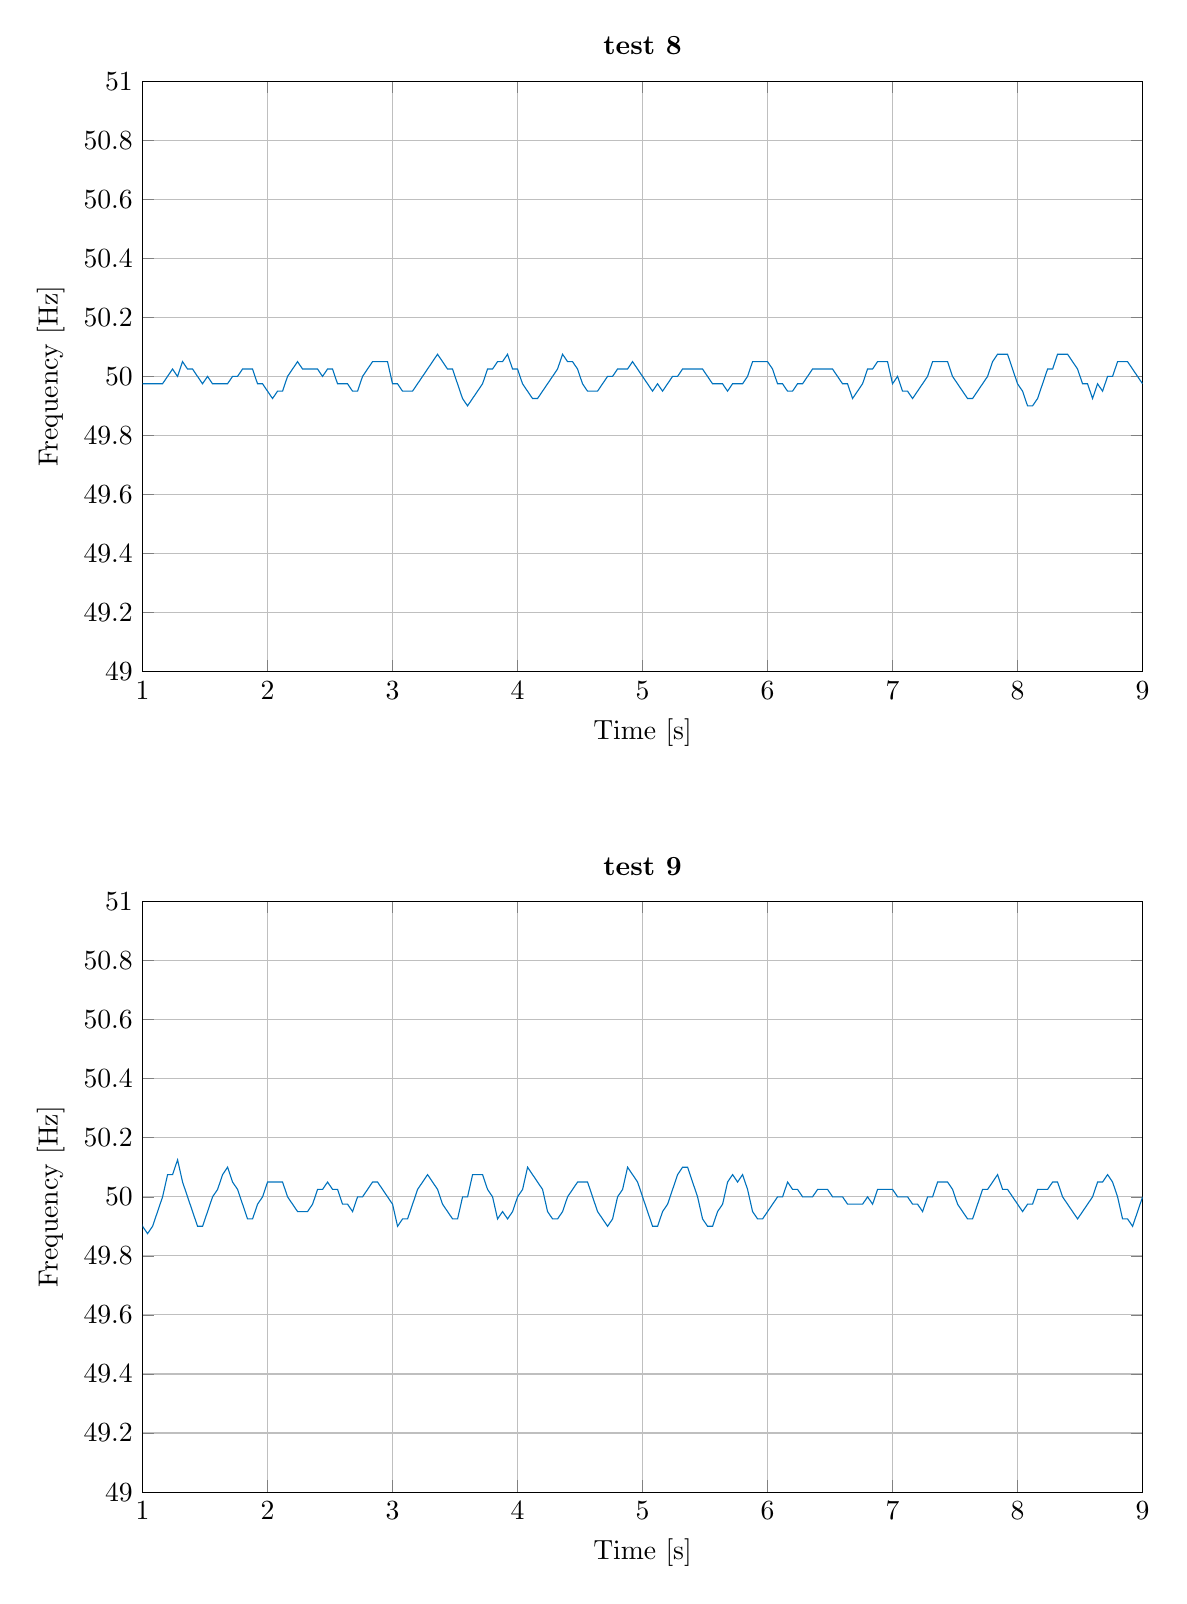
\begin{tikzpicture}

\begin{axis}[%
width=5in,
height=2.953in,
at={(1.142in,5.054in)},
scale only axis,
xmin=1,
xmax=9,
xlabel={Time [s]},
xmajorgrids,
ymin=49,
ymax=51,
ylabel={Frequency [Hz]},
ymajorgrids,
axis background/.style={fill=white},
title style={font=\bfseries},
title={test 8}
]
\addplot [color=mycolor1,solid,forget plot]
  table[row sep=crcr]{%
0.9998	49.9750124937531\\
1.03982	49.9750124937532\\
1.07984	49.9750124937532\\
1.11986	49.9750124937532\\
1.15988	49.9750124937529\\
1.1999	50\\
1.2399	50.0250125062532\\
1.27988	50\\
1.31988	50.0500500500501\\
1.35984	50.0250125062532\\
1.39982	50.025012506253\\
1.4398	50.0000000000002\\
1.4798	49.9750124937529\\
1.51982	50.0000000000002\\
1.55982	49.9750124937529\\
1.59984	49.9750124937532\\
1.63986	49.9750124937532\\
1.67988	49.9750124937532\\
1.7199	50\\
1.7599	50\\
1.7999	50.0250125062532\\
1.83988	50.025012506253\\
1.87986	50.0250125062532\\
1.91984	49.9750124937529\\
1.95986	49.9750124937532\\
1.99988	49.9500499500499\\
2.03992	49.9251123315028\\
2.07998	49.9500499500501\\
2.12002	49.9500499500501\\
2.16006	50\\
2.20006	50.0250125062532\\
2.24004	50.0500500500498\\
2.28	50.0250125062532\\
2.31998	50.0250125062532\\
2.35996	50.0250125062527\\
2.39994	50.0250125062532\\
2.43992	50\\
2.47992	50.0250125062532\\
2.5199	50.0250125062532\\
2.55988	49.9750124937529\\
2.5999	49.9750124937535\\
2.63992	49.9750124937529\\
2.67994	49.9500499500501\\
2.71998	49.9500499500496\\
2.76002	50\\
2.80002	50.0250125062532\\
2.84	50.0500500500503\\
2.87996	50.0500500500498\\
2.91992	50.0500500500503\\
2.95988	50.0500500500498\\
2.99984	49.9750124937535\\
3.03986	49.9750124937529\\
3.07988	49.9500499500501\\
3.11992	49.9500499500496\\
3.15996	49.9500499500501\\
3.2	49.9750124937529\\
3.24002	50.0000000000005\\
3.28002	50.0250125062527\\
3.32	50.0500500500503\\
3.35996	50.0751126690034\\
3.3999	50.0500500500498\\
3.43986	50.0250125062532\\
3.47984	50.0250125062532\\
3.51982	49.9750124937529\\
3.55984	49.9251123315028\\
3.5999	49.9001996007988\\
3.63998	49.9251123315028\\
3.68004	49.9500499500496\\
3.72008	49.9750124937535\\
3.7601	50.0250125062532\\
3.80008	50.0250125062527\\
3.84006	50.0500500500503\\
3.88002	50.0500500500498\\
3.91998	50.075112669004\\
3.95992	50.0250125062527\\
3.9999	50.0250125062538\\
4.03988	49.9750124937529\\
4.0799	49.9500499500496\\
4.11994	49.9251123315033\\
4.16	49.9251123315022\\
4.20006	49.9500499500496\\
4.2401	49.975012493754\\
4.28012	50\\
4.32012	50.0250125062532\\
4.3601	50.0751126690028\\
4.40004	50.0500500500503\\
4.44	50.0500500500503\\
4.47996	50.0250125062532\\
4.51994	49.9750124937529\\
4.55996	49.9500499500496\\
4.6	49.9500499500496\\
4.64004	49.9500499500507\\
4.68008	49.9750124937529\\
4.7201	50\\
4.7601	50\\
4.8001	50.0250125062532\\
4.84008	50.0250125062532\\
4.88006	50.0250125062532\\
4.92004	50.0500500500492\\
4.96	50.0250125062532\\
4.99998	50\\
5.03998	49.975012493754\\
5.08	49.9500499500496\\
5.12004	49.9750124937529\\
5.16006	49.9500499500496\\
5.2001	49.975012493754\\
5.24012	50\\
5.28012	50\\
5.32012	50.0250125062532\\
5.3601	50.0250125062532\\
5.40008	50.0250125062521\\
5.44006	50.0250125062532\\
5.48004	50.0250125062532\\
5.52002	50\\
5.56002	49.9750124937529\\
5.60004	49.975012493754\\
5.64006	49.9750124937529\\
5.68008	49.9500499500496\\
5.72012	49.9750124937529\\
5.76014	49.975012493754\\
5.80016	49.9750124937529\\
5.84018	50\\
5.88018	50.0500500500503\\
5.92014	50.0500500500492\\
5.9601	50.0500500500503\\
6.00006	50.0500500500503\\
6.04002	50.0250125062532\\
6.08	49.9750124937529\\
6.12002	49.9750124937529\\
6.16004	49.9500499500496\\
6.20008	49.9500499500507\\
6.24012	49.9750124937529\\
6.28014	49.9750124937529\\
6.32016	50\\
6.36016	50.0250125062532\\
6.40014	50.0250125062532\\
6.44012	50.0250125062532\\
6.4801	50.0250125062532\\
6.52008	50.0250125062532\\
6.56006	50\\
6.60006	49.9750124937529\\
6.64008	49.9750124937529\\
6.6801	49.9251123315033\\
6.72016	49.9500499500496\\
6.7602	49.9750124937529\\
6.80022	50.0250125062532\\
6.8402	50.0250125062532\\
6.88018	50.0500500500503\\
6.92014	50.0500500500492\\
6.9601	50.0500500500503\\
7.00006	49.9750124937529\\
7.04008	50\\
7.08008	49.9500499500507\\
7.12012	49.9500499500496\\
7.16016	49.9251123315033\\
7.20022	49.9500499500496\\
7.24026	49.9750124937529\\
7.28028	50\\
7.32028	50.0500500500503\\
7.36024	50.0500500500503\\
7.4002	50.0500500500492\\
7.44016	50.0500500500503\\
7.48012	50\\
7.52012	49.9750124937529\\
7.56014	49.9500499500507\\
7.60018	49.9251123315022\\
7.64024	49.9251123315033\\
7.6803	49.9500499500496\\
7.72034	49.9750124937529\\
7.76036	50\\
7.80036	50.0500500500503\\
7.84032	50.075112669004\\
7.88026	50.0751126690028\\
7.9202	50.075112669004\\
7.96014	50.0250125062532\\
8.00012	49.9750124937529\\
8.04014	49.9500499500507\\
8.08018	49.9001996007966\\
8.12026	49.9001996007988\\
8.16034	49.9251123315022\\
8.2004	49.9750124937551\\
8.24042	50.0250125062532\\
8.2804	50.025012506251\\
8.32038	50.075112669004\\
8.36032	50.075112669004\\
8.40026	50.075112669004\\
8.4402	50.0500500500492\\
8.48016	50.0250125062532\\
8.52014	49.9750124937529\\
8.56016	49.9750124937529\\
8.60018	49.9251123315044\\
8.64024	49.9750124937529\\
8.68026	49.9500499500485\\
8.7203	50.0000000000011\\
8.7603	49.9999999999988\\
8.8003	50.0500500500514\\
8.84026	50.0500500500492\\
8.88022	50.0500500500514\\
8.92018	50.0250125062532\\
8.96016	49.9999999999988\\
9.00016	49.9750124937529\\
};
\end{axis}

\begin{axis}[%
width=5in,
height=2.953in,
at={(1.142in,0.952in)},
scale only axis,
xmin=1,
xmax=9,
xlabel={Time [s]},
xmajorgrids,
ymin=49,
ymax=51,
ylabel={Frequency [Hz]},
ymajorgrids,
axis background/.style={fill=white},
title style={font=\bfseries},
title={test 9}
]
\addplot [color=mycolor1,solid,forget plot]
  table[row sep=crcr]{%
0.96004	49.9750124937531\\
1.00006	49.9001996007985\\
1.04014	49.8753117206982\\
1.08024	49.9001996007983\\
1.12032	49.9500499500501\\
1.16036	50\\
1.20036	50.0751126690034\\
1.2403	50.0751126690037\\
1.28024	50.125313283208\\
1.32014	50.0500500500501\\
1.3601	50\\
1.4001	49.9500499500499\\
1.44014	49.9001996007985\\
1.48022	49.9001996007985\\
1.5203	49.9500499500499\\
1.56034	50\\
1.60034	50.0250125062532\\
1.64032	50.0751126690034\\
1.68026	50.1002004008017\\
1.72018	50.0500500500501\\
1.76014	50.025012506253\\
1.80012	49.9750124937532\\
1.84014	49.9251123315028\\
1.8802	49.9251123315028\\
1.92026	49.9750124937532\\
1.96028	50.0000000000002\\
2.00028	50.0500500500498\\
2.04024	50.0500500500503\\
2.0802	50.0500500500498\\
2.12016	50.0500500500503\\
2.16012	50\\
2.20012	49.9750124937529\\
2.24014	49.9500499500501\\
2.28018	49.9500499500496\\
2.32022	49.9500499500501\\
2.36026	49.9750124937529\\
2.40028	50.0250125062532\\
2.44026	50.0250125062532\\
2.48024	50.0500500500498\\
2.5202	50.0250125062532\\
2.56018	50.0250125062532\\
2.60016	49.9750124937529\\
2.64018	49.9750124937535\\
2.6802	49.9500499500501\\
2.72024	50\\
2.76024	50\\
2.80024	50.0250125062527\\
2.84022	50.0500500500503\\
2.88018	50.0500500500498\\
2.92014	50.0250125062532\\
2.96012	50\\
3.00012	49.9750124937535\\
3.04014	49.9001996007983\\
3.08022	49.9251123315028\\
3.12028	49.9251123315028\\
3.16034	49.9750124937529\\
3.20036	50.0250125062532\\
3.24034	50.0500500500503\\
3.2803	50.0751126690034\\
3.32024	50.0500500500498\\
3.3602	50.0250125062532\\
3.40018	49.9750124937535\\
3.4402	49.9500499500496\\
3.48024	49.9251123315028\\
3.5203	49.9251123315028\\
3.56036	50\\
3.60036	50\\
3.64036	50.075112669004\\
3.6803	50.0751126690034\\
3.72024	50.0751126690034\\
3.76018	50.0250125062532\\
3.80016	50\\
3.84016	49.9251123315028\\
3.88022	49.9500499500496\\
3.92026	49.9251123315028\\
3.96032	49.9500499500501\\
4.00036	50\\
4.04036	50.0250125062532\\
4.08034	50.1002004008011\\
4.12026	50.075112669004\\
4.1602	50.0500500500503\\
4.20016	50.0250125062532\\
4.24014	49.9500499500496\\
4.28018	49.9251123315033\\
4.32024	49.9251123315022\\
4.3603	49.9500499500496\\
4.40034	50\\
4.44034	50.0250125062532\\
4.48032	50.0500500500503\\
4.52028	50.0500500500503\\
4.56024	50.0500500500503\\
4.6002	50\\
4.6402	49.9500499500496\\
4.68024	49.9251123315022\\
4.7203	49.9001996007988\\
4.76038	49.9251123315033\\
4.80044	50\\
4.84044	50.0250125062521\\
4.88042	50.1002004008022\\
4.92034	50.075112669004\\
4.96028	50.0500500500492\\
5.00024	50\\
5.04024	49.9500499500507\\
5.08028	49.9001996007977\\
5.12036	49.9001996007988\\
5.16044	49.9500499500496\\
5.20048	49.9750124937529\\
5.2405	50.0250125062532\\
5.28048	50.075112669004\\
5.32042	50.1002004008011\\
5.36034	50.1002004008022\\
5.40026	50.0500500500503\\
5.44022	50\\
5.48022	49.9251123315022\\
5.52028	49.9001996007988\\
5.56036	49.9001996007977\\
5.60044	49.9500499500507\\
5.64048	49.9750124937529\\
5.6805	50.0500500500503\\
5.72046	50.0751126690028\\
5.7604	50.0500500500503\\
5.80036	50.075112669004\\
5.8403	50.0250125062532\\
5.88028	49.9500499500496\\
5.92032	49.9251123315022\\
5.96038	49.9251123315033\\
6.00044	49.9500499500496\\
6.04048	49.9750124937529\\
6.0805	50\\
6.1205	50\\
6.1605	50.0500500500503\\
6.20046	50.0250125062532\\
6.24044	50.0250125062532\\
6.28042	50\\
6.32042	50\\
6.36042	50\\
6.40042	50.0250125062532\\
6.4404	50.0250125062532\\
6.48038	50.0250125062532\\
6.52036	50\\
6.56036	50\\
6.60036	50\\
6.64036	49.9750124937529\\
6.68038	49.9750124937529\\
6.7204	49.975012493754\\
6.76042	49.9750124937529\\
6.80044	50\\
6.84044	49.9750124937529\\
6.88046	50.0250125062532\\
6.92044	50.0250125062532\\
6.96042	50.0250125062532\\
7.0004	50.0250125062532\\
7.04038	50\\
7.08038	50\\
7.12038	50\\
7.16038	49.9750124937529\\
7.2004	49.9750124937529\\
7.24042	49.9500499500496\\
7.28046	50\\
7.32046	50\\
7.36046	50.0500500500503\\
7.40042	50.0500500500503\\
7.44038	50.0500500500503\\
7.48034	50.0250125062532\\
7.52032	49.9750124937529\\
7.56034	49.9500499500496\\
7.60038	49.9251123315033\\
7.64044	49.9251123315022\\
7.6805	49.9750124937529\\
7.72052	50.0250125062532\\
7.7605	50.0250125062532\\
7.80048	50.0500500500503\\
7.84044	50.0751126690028\\
7.88038	50.0250125062532\\
7.92036	50.0250125062532\\
7.96034	50\\
8.00034	49.9750124937529\\
8.04036	49.9500499500507\\
8.0804	49.9750124937529\\
8.12042	49.9750124937529\\
8.16044	50.0250125062532\\
8.20042	50.0250125062532\\
8.2404	50.0250125062532\\
8.28038	50.0500500500492\\
8.32034	50.0500500500514\\
8.3603	49.9999999999988\\
8.4003	49.9750124937529\\
8.44032	49.9500499500507\\
8.48036	49.9251123315022\\
8.52042	49.9500499500507\\
8.56046	49.9750124937529\\
8.60048	50.0000000000011\\
8.64048	50.0500500500492\\
8.68044	50.0500500500492\\
8.7204	50.075112669004\\
8.76034	50.0500500500492\\
8.8003	50.0000000000011\\
8.8403	49.9251123315022\\
8.88036	49.9251123315022\\
8.92042	49.9001996007988\\
8.9605	49.9500499500507\\
9.00054	49.9999999999988\\
};
\end{axis}
\end{tikzpicture}%
\caption{Steady state frequency output of the genset at 10 kW load.}
\label{fig:test8-9steadyfrequency10kw}
\end{figure}

\begin{figure}[H]
\centering
% This file was created by matlab2tikz.
%
%The latest updates can be retrieved from
%  http://www.mathworks.com/matlabcentral/fileexchange/22022-matlab2tikz-matlab2tikz
%where you can also make suggestions and rate matlab2tikz.
%
\definecolor{mycolor1}{rgb}{0.00000,0.44700,0.74100}%
%
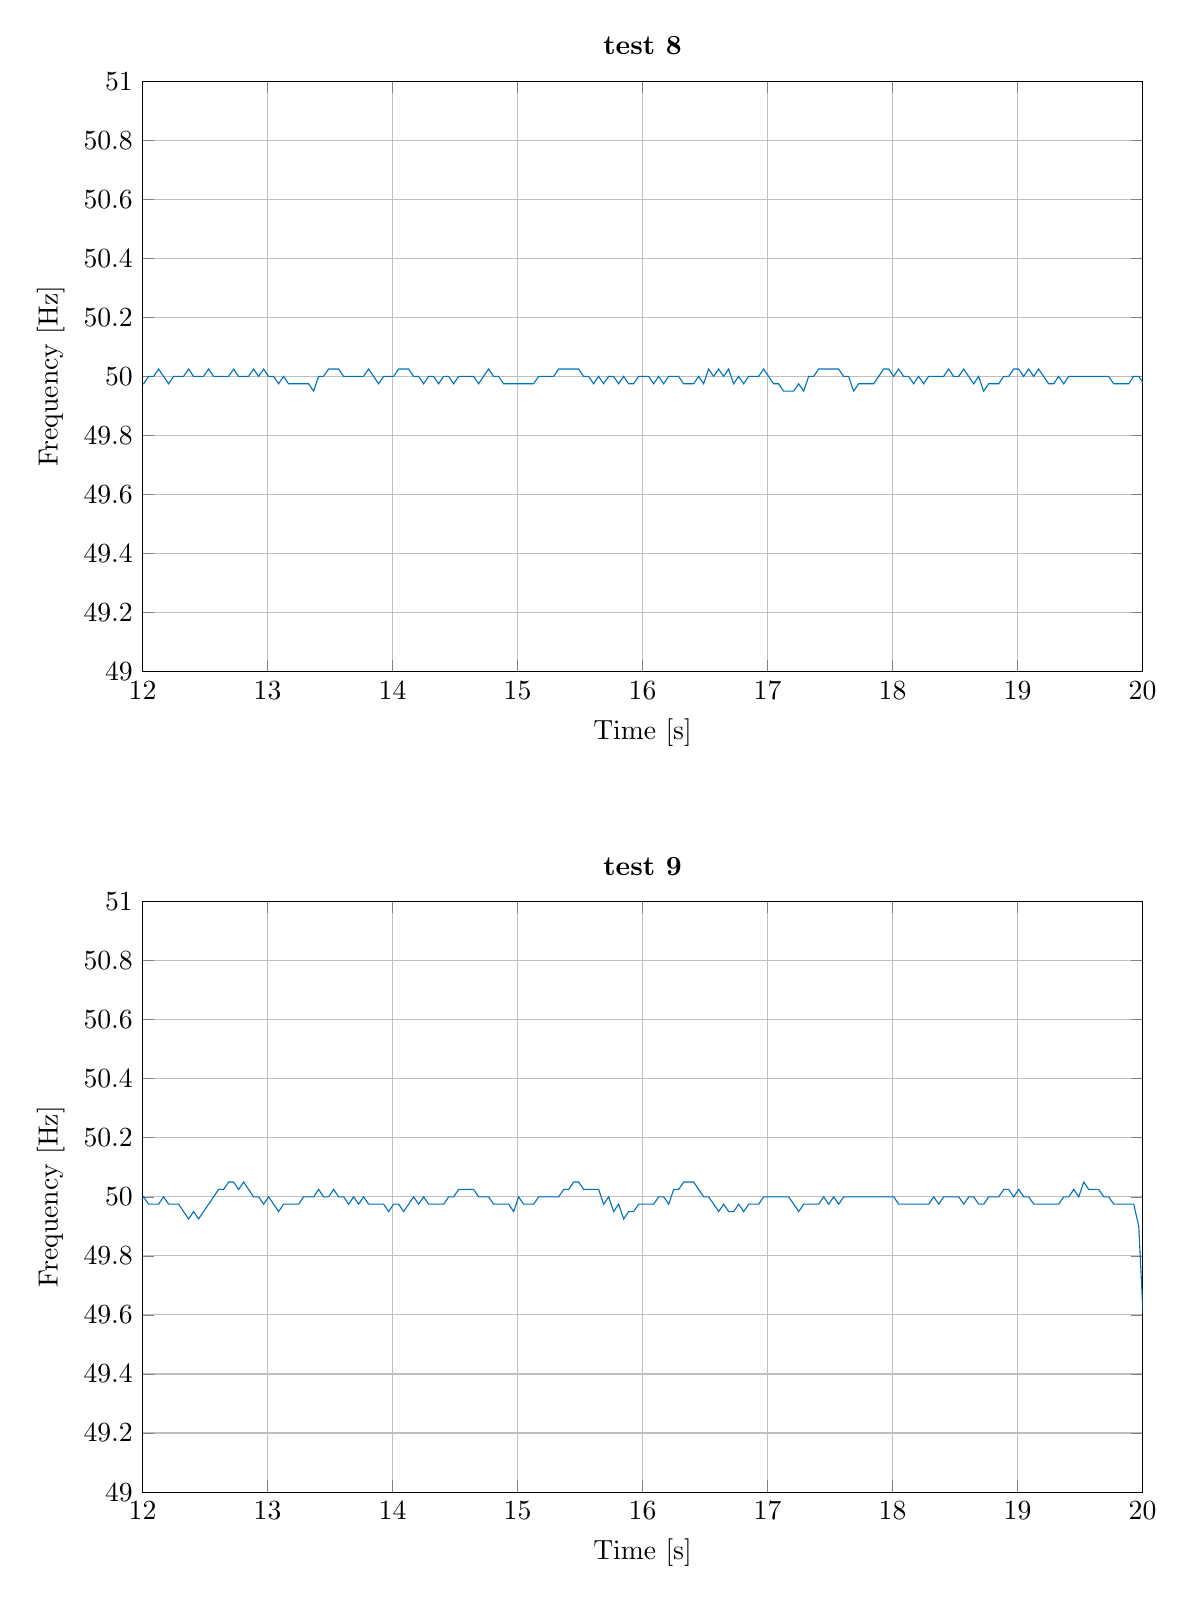
\begin{tikzpicture}

\begin{axis}[%
width=5in,
height=2.953in,
at={(1.142in,5.054in)},
scale only axis,
xmin=12,
xmax=20,
xlabel={Time [s]},
xmajorgrids,
ymin=49,
ymax=51,
ylabel={Frequency [Hz]},
ymajorgrids,
axis background/.style={fill=white},
title style={font=\bfseries},
title={test 8}
]
\addplot [color=mycolor1,solid,forget plot]
  table[row sep=crcr]{%
11.96844	49.9750124937529\\
12.00846	49.9750124937529\\
12.04848	50.0000000000011\\
12.08848	49.9999999999988\\
12.12848	50.0250125062532\\
12.16846	50.0000000000011\\
12.20846	49.9750124937529\\
12.24848	50.0000000000011\\
12.28848	49.9999999999988\\
12.32848	50.0000000000011\\
12.36848	50.0250125062532\\
12.40846	49.9999999999988\\
12.44846	50.0000000000011\\
12.48846	49.9999999999988\\
12.52846	50.0250125062532\\
12.56844	50.0000000000011\\
12.60844	49.9999999999988\\
12.64844	50.0000000000011\\
12.68844	49.9999999999988\\
12.72844	50.0250125062532\\
12.76842	50.0000000000011\\
12.80842	49.9999999999988\\
12.84842	50.0000000000011\\
12.88842	50.0250125062532\\
12.9284	49.9999999999988\\
12.9684	50.0250125062532\\
13.00838	50.0000000000011\\
13.04838	49.9999999999988\\
13.08838	49.9750124937529\\
13.1284	50.0000000000011\\
13.1684	49.9750124937529\\
13.20842	49.9750124937529\\
13.24844	49.9750124937529\\
13.28846	49.9750124937529\\
13.32848	49.9750124937529\\
13.3685	49.9500499500507\\
13.40854	49.9999999999988\\
13.44854	50.0000000000011\\
13.48854	50.0250125062532\\
13.52852	50.0250125062532\\
13.5685	50.0250125062532\\
13.60848	49.9999999999988\\
13.64848	50.0000000000011\\
13.68848	49.9999999999988\\
13.72848	50.0000000000011\\
13.76848	49.9999999999988\\
13.80848	50.0250125062532\\
13.84846	50.0000000000011\\
13.88846	49.9750124937529\\
13.92848	49.9999999999988\\
13.96848	50.0000000000011\\
14.00848	49.9999999999988\\
14.04848	50.0250125062532\\
14.08846	50.0250125062532\\
14.12844	50.0250125062532\\
14.16842	50.0000000000011\\
14.20842	49.9999999999988\\
14.24842	49.9750124937529\\
14.28844	50.0000000000011\\
14.32844	50.0000000000011\\
14.36844	49.9750124937529\\
14.40846	49.9999999999988\\
14.44846	50.0000000000011\\
14.48846	49.9750124937529\\
14.52848	49.9999999999988\\
14.56848	50.0000000000011\\
14.60848	49.9999999999988\\
14.64848	50.0000000000011\\
14.68848	49.9750124937529\\
14.7285	49.9999999999988\\
14.7685	50.0250125062532\\
14.80848	50.0000000000011\\
14.84848	49.9999999999988\\
14.88848	49.9750124937551\\
14.9285	49.9750124937529\\
14.96852	49.9750124937529\\
15.00854	49.9750124937529\\
15.04856	49.9750124937529\\
15.08858	49.9750124937529\\
15.1286	49.9750124937529\\
15.16862	50.0000000000011\\
15.20862	49.9999999999988\\
15.24862	50.0000000000011\\
15.28862	49.9999999999988\\
15.32862	50.0250125062532\\
15.3686	50.0250125062532\\
15.40858	50.0250125062532\\
15.44856	50.0250125062532\\
15.48854	50.0250125062532\\
15.52852	49.9999999999988\\
15.56852	50.0000000000011\\
15.60852	49.9750124937529\\
15.64854	50.0000000000011\\
15.68854	49.9750124937529\\
15.72856	49.9999999999988\\
15.76856	50.0000000000011\\
15.80856	49.9750124937529\\
15.84858	49.9999999999988\\
15.88858	49.9750124937529\\
15.9286	49.9750124937551\\
15.96862	50.0000000000011\\
16.00862	49.9999999999966\\
16.04862	50.0000000000011\\
16.08862	49.9750124937551\\
16.12864	49.9999999999966\\
16.16864	49.9750124937551\\
16.20866	50.0000000000011\\
16.24866	49.9999999999966\\
16.28866	50.0000000000011\\
16.32866	49.9750124937551\\
16.36868	49.9750124937507\\
16.4087	49.9750124937551\\
16.44872	50.0000000000011\\
16.48872	49.9750124937507\\
16.52874	50.0250125062532\\
16.56872	50.0000000000011\\
16.60872	50.0250125062532\\
16.6487	50.0000000000011\\
16.6887	50.0250125062532\\
16.72868	49.9750124937507\\
16.7687	50.0000000000011\\
16.8087	49.9750124937507\\
16.84872	50.0000000000011\\
16.88872	50.0000000000011\\
16.92872	50.0000000000011\\
16.96872	50.0250125062532\\
17.0087	49.9999999999966\\
17.0487	49.9750124937551\\
17.08872	49.9750124937551\\
17.12874	49.9500499500485\\
17.16878	49.9500499500485\\
17.20882	49.9500499500529\\
17.24886	49.9750124937507\\
17.28888	49.9500499500485\\
17.32892	50.0000000000011\\
17.36892	50.0000000000011\\
17.40892	50.0250125062532\\
17.4489	50.0250125062532\\
17.48888	50.0250125062532\\
17.52886	50.0250125062532\\
17.56884	50.0250125062532\\
17.60882	50.0000000000011\\
17.64882	49.9999999999966\\
17.68882	49.9500499500529\\
17.72886	49.9750124937507\\
17.76888	49.9750124937551\\
17.8089	49.9750124937507\\
17.84892	49.9750124937551\\
17.88894	50.0000000000011\\
17.92894	50.0250125062532\\
17.96892	50.0250125062532\\
18.0089	49.9999999999966\\
18.0489	50.0250125062532\\
18.08888	50.0000000000011\\
18.12888	50.0000000000011\\
18.16888	49.9750124937507\\
18.2089	50.0000000000011\\
18.2489	49.9750124937551\\
18.28892	49.9999999999966\\
18.32892	50.0000000000011\\
18.36892	50.0000000000011\\
18.40892	50.0000000000011\\
18.44892	50.0250125062532\\
18.4889	49.9999999999966\\
18.5289	50.0000000000011\\
18.5689	50.0250125062532\\
18.60888	50.0000000000011\\
18.64888	49.9750124937551\\
18.6889	49.9999999999966\\
18.7289	49.9500499500529\\
18.76894	49.9750124937507\\
18.80896	49.9750124937551\\
18.84898	49.9750124937507\\
18.889	50.0000000000011\\
18.929	50.0000000000011\\
18.969	50.0250125062532\\
19.00898	50.0250125062532\\
19.04896	50.0000000000011\\
19.08896	50.0250125062488\\
19.12894	50.0000000000011\\
19.16894	50.0250125062532\\
19.20892	50.0000000000011\\
19.24892	49.9750124937551\\
19.28894	49.9750124937507\\
19.32896	50.0000000000011\\
19.36896	49.9750124937507\\
19.40898	50.0000000000011\\
19.44898	50.0000000000011\\
19.48898	50.0000000000011\\
19.52898	49.9999999999966\\
19.56898	50.0000000000011\\
19.60898	50.0000000000011\\
19.64898	50.0000000000011\\
19.68898	49.9999999999966\\
19.72898	50.0000000000011\\
19.76898	49.9750124937551\\
19.809	49.9750124937507\\
19.84902	49.9750124937551\\
19.88904	49.9750124937507\\
19.92906	50.0000000000011\\
19.96906	50.0000000000011\\
20.00906	49.9750124937507\\
};
\end{axis}

\begin{axis}[%
width=5in,
height=2.953in,
at={(1.142in,0.952in)},
scale only axis,
xmin=12,
xmax=20,
xlabel={Time [s]},
xmajorgrids,
ymin=49,
ymax=51,
ylabel={Frequency [Hz]},
ymajorgrids,
axis background/.style={fill=white},
title style={font=\bfseries},
title={test 9}
]
\addplot [color=mycolor1,solid,forget plot]
  table[row sep=crcr]{%
11.96826	49.9750124937529\\
12.00828	50.0000000000011\\
12.04828	49.9750124937529\\
12.0883	49.9750124937529\\
12.12832	49.9750124937529\\
12.16834	49.9999999999988\\
12.20834	49.9750124937551\\
12.24836	49.9750124937529\\
12.28838	49.9750124937529\\
12.3284	49.9500499500485\\
12.36844	49.9251123315044\\
12.4085	49.9500499500485\\
12.44854	49.9251123315044\\
12.4886	49.9500499500485\\
12.52864	49.9750124937529\\
12.56866	50.0000000000011\\
12.60866	50.0250125062532\\
12.64864	50.0250125062532\\
12.68862	50.0500500500492\\
12.72858	50.0500500500514\\
12.76854	50.025012506251\\
12.80852	50.0500500500514\\
12.84848	50.0250125062532\\
12.88846	49.9999999999988\\
12.92846	50.0000000000011\\
12.96846	49.9750124937529\\
13.00848	49.9999999999988\\
13.04848	49.9750124937551\\
13.0885	49.9500499500485\\
13.12854	49.9750124937529\\
13.16856	49.9750124937529\\
13.20858	49.9750124937529\\
13.2486	49.9750124937551\\
13.28862	49.9999999999988\\
13.32862	50.0000000000011\\
13.36862	49.9999999999988\\
13.40862	50.0250125062532\\
13.4486	50.0000000000011\\
13.4886	49.9999999999988\\
13.5286	50.0250125062532\\
13.56858	50.0000000000011\\
13.60858	49.9999999999988\\
13.64858	49.9750124937529\\
13.6886	50.0000000000011\\
13.7286	49.9750124937529\\
13.76862	49.9999999999988\\
13.80862	49.9750124937529\\
13.84864	49.9750124937551\\
13.88866	49.9750124937529\\
13.92868	49.9750124937529\\
13.9687	49.9500499500485\\
14.00874	49.9750124937551\\
14.04876	49.9750124937529\\
14.08878	49.9500499500485\\
14.12882	49.9750124937529\\
14.16884	50.0000000000011\\
14.20884	49.9750124937529\\
14.24886	50.0000000000011\\
14.28886	49.9750124937529\\
14.32888	49.9750124937529\\
14.3689	49.9750124937529\\
14.40892	49.9750124937529\\
14.44894	49.9999999999988\\
14.48894	50.0000000000011\\
14.52894	50.0250125062532\\
14.56892	50.0250125062532\\
14.6089	50.0250125062532\\
14.64888	50.0250125062532\\
14.68886	49.9999999999988\\
14.72886	50.0000000000011\\
14.76886	49.9999999999988\\
14.80886	49.9750124937529\\
14.84888	49.9750124937529\\
14.8889	49.9750124937551\\
14.92892	49.9750124937529\\
14.96894	49.9500499500485\\
15.00898	50.0000000000011\\
15.04898	49.9750124937529\\
15.089	49.9750124937529\\
15.12902	49.9750124937529\\
15.16904	50.0000000000011\\
15.20904	49.9999999999988\\
15.24904	50.0000000000011\\
15.28904	49.9999999999988\\
15.32904	50.0000000000011\\
15.36904	50.0250125062532\\
15.40902	50.0250125062532\\
15.449	50.0500500500492\\
15.48896	50.0500500500492\\
15.52892	50.0250125062532\\
15.5689	50.0250125062532\\
15.60888	50.0250125062532\\
15.64886	50.0250125062532\\
15.68884	49.9750124937529\\
15.72886	50.0000000000011\\
15.76886	49.9500499500507\\
15.8089	49.9750124937529\\
15.84892	49.9251123315022\\
15.88898	49.9500499500507\\
15.92902	49.9500499500485\\
15.96906	49.9750124937551\\
16.00908	49.9750124937507\\
16.0491	49.9750124937551\\
16.08912	49.9750124937507\\
16.12914	50.0000000000011\\
16.16914	50.0000000000011\\
16.20914	49.9750124937507\\
16.24916	50.0250125062532\\
16.28914	50.0250125062532\\
16.32912	50.0500500500492\\
16.36908	50.0500500500537\\
16.40904	50.0500500500492\\
16.449	50.0250125062532\\
16.48898	50.0000000000011\\
16.52898	49.9999999999966\\
16.56898	49.9750124937551\\
16.609	49.9500499500485\\
16.64904	49.9750124937551\\
16.68906	49.9500499500485\\
16.7291	49.9500499500485\\
16.76914	49.9750124937551\\
16.80916	49.9500499500485\\
16.8492	49.9750124937551\\
16.88922	49.9750124937507\\
16.92924	49.9750124937551\\
16.96926	50.0000000000011\\
17.00926	50.0000000000011\\
17.04926	49.9999999999966\\
17.08926	50.0000000000011\\
17.12926	50.0000000000011\\
17.16926	50.0000000000011\\
17.20926	49.9750124937507\\
17.24928	49.9500499500485\\
17.28932	49.9750124937551\\
17.32934	49.9750124937551\\
17.36936	49.9750124937507\\
17.40938	49.9750124937551\\
17.4494	49.9999999999966\\
17.4894	49.9750124937551\\
17.52942	50.0000000000011\\
17.56942	49.9750124937507\\
17.60944	50.0000000000011\\
17.64944	50.0000000000011\\
17.68944	50.0000000000011\\
17.72944	49.9999999999966\\
17.76944	50.0000000000011\\
17.80944	50.0000000000011\\
17.84944	50.0000000000011\\
17.88944	49.9999999999966\\
17.92944	50.0000000000011\\
17.96944	50.0000000000011\\
18.00944	50.0000000000011\\
18.04944	49.9750124937507\\
18.08946	49.9750124937551\\
18.12948	49.9750124937507\\
18.1695	49.9750124937551\\
18.20952	49.9750124937507\\
18.24954	49.9750124937551\\
18.28956	49.9750124937507\\
18.32958	50.0000000000011\\
18.36958	49.9750124937551\\
18.4096	50.0000000000011\\
18.4496	49.9999999999966\\
18.4896	50.0000000000011\\
18.5296	50.0000000000011\\
18.5696	49.9750124937507\\
18.60962	50.0000000000011\\
18.64962	50.0000000000011\\
18.68962	49.9750124937507\\
18.72964	49.9750124937551\\
18.76966	50.0000000000011\\
18.80966	49.9999999999966\\
18.84966	50.0000000000011\\
18.88966	50.0250125062532\\
18.92964	50.0250125062532\\
18.96962	50.0000000000011\\
19.00962	50.0250125062532\\
19.0496	50.0000000000011\\
19.0896	49.9999999999966\\
19.1296	49.9750124937551\\
19.16962	49.9750124937551\\
19.20964	49.9750124937507\\
19.24966	49.9750124937551\\
19.28968	49.9750124937507\\
19.3297	49.9750124937551\\
19.36972	50.0000000000011\\
19.40972	49.9999999999966\\
19.44972	50.0250125062532\\
19.4897	50.0000000000011\\
19.5297	50.0500500500492\\
19.56966	50.0250125062532\\
19.60964	50.0250125062532\\
19.64962	50.0250125062532\\
19.6896	50.0000000000011\\
19.7296	50.0000000000011\\
19.7696	49.9750124937507\\
19.80962	49.9750124937551\\
19.84964	49.9750124937507\\
19.88966	49.9750124937551\\
19.92968	49.9750124937507\\
19.9697	49.9001996007988\\
20.00978	49.5540138751242\\
};
\end{axis}
\end{tikzpicture}%
\caption{Steady state frequency output of the genset at 20 kW load.}
\label{fig:test8-9steadyfrequency20kw}
\end{figure}

\begin{figure}[H]
\centering
% This file was created by matlab2tikz.
%
%The latest updates can be retrieved from
%  http://www.mathworks.com/matlabcentral/fileexchange/22022-matlab2tikz-matlab2tikz
%where you can also make suggestions and rate matlab2tikz.
%
\definecolor{mycolor1}{rgb}{0.00000,0.44700,0.74100}%
%
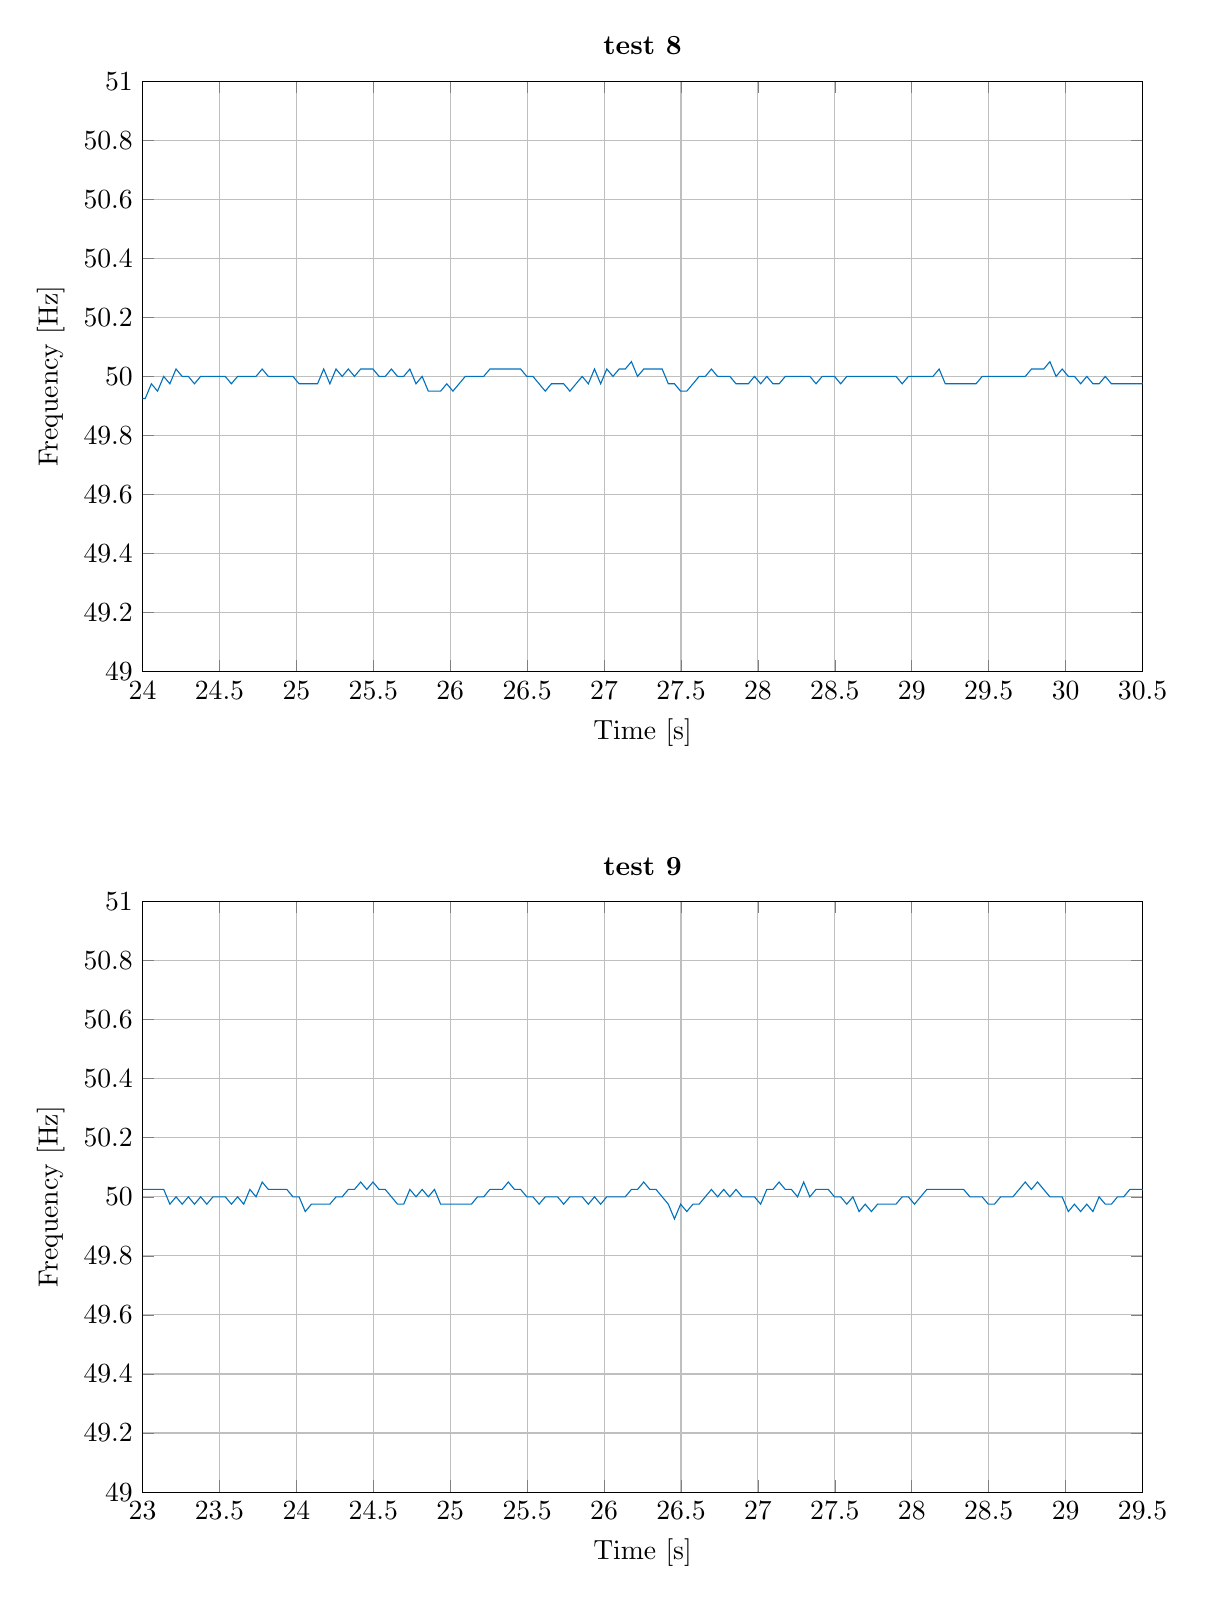
\begin{tikzpicture}

\begin{axis}[%
width=5in,
height=2.953in,
at={(1.142in,5.054in)},
scale only axis,
xmin=24,
xmax=30.5,
xlabel={Time [s]},
xmajorgrids,
ymin=49,
ymax=51,
ylabel={Frequency [Hz]},
ymajorgrids,
axis background/.style={fill=white},
title style={font=\bfseries},
title={test 8}
]
\addplot [color=mycolor1,solid,forget plot]
  table[row sep=crcr]{%
23.97732	49.9251123315022\\
24.01738	49.9251123315066\\
24.05744	49.9750124937507\\
24.09746	49.9500499500485\\
24.1375	50.0000000000011\\
24.1775	49.9750124937551\\
24.21752	50.0250125062532\\
24.2575	49.9999999999966\\
24.2975	50.0000000000011\\
24.3375	49.9750124937551\\
24.37752	50.0000000000011\\
24.41752	49.9999999999966\\
24.45752	50.0000000000011\\
24.49752	50.0000000000011\\
24.53752	50.0000000000011\\
24.57752	49.9750124937507\\
24.61754	50.0000000000011\\
24.65754	50.0000000000011\\
24.69754	49.9999999999966\\
24.73754	50.0000000000011\\
24.77754	50.0250125062532\\
24.81752	50.0000000000011\\
24.85752	50.0000000000011\\
24.89752	49.9999999999966\\
24.93752	50.0000000000011\\
24.97752	50.0000000000011\\
25.01752	49.9750124937507\\
25.05754	49.9750124937551\\
25.09756	49.9750124937551\\
25.13758	49.9750124937507\\
25.1776	50.0250125062532\\
25.21758	49.9750124937551\\
25.2576	50.0250125062532\\
25.29758	49.9999999999966\\
25.33758	50.0250125062532\\
25.37756	50.0000000000011\\
25.41756	50.0250125062532\\
25.45754	50.0250125062532\\
25.49752	50.0250125062532\\
25.5375	50.0000000000011\\
25.5775	50.0000000000011\\
25.6175	50.0250125062532\\
25.65748	49.9999999999966\\
25.69748	50.0000000000011\\
25.73748	50.0250125062532\\
25.77746	49.9750124937551\\
25.81748	49.9999999999966\\
25.85748	49.9500499500529\\
25.89752	49.9500499500485\\
25.93756	49.9500499500485\\
25.9776	49.9750124937551\\
26.01762	49.9500499500485\\
26.05766	49.9750124937551\\
26.09768	50.0000000000011\\
26.13768	49.9999999999966\\
26.17768	50.0000000000011\\
26.21768	50.0000000000011\\
26.25768	50.0250125062532\\
26.29766	50.0250125062532\\
26.33764	50.0250125062532\\
26.37762	50.0250125062532\\
26.4176	50.0250125062532\\
26.45758	50.0250125062532\\
26.49756	49.9999999999966\\
26.53756	50.0000000000011\\
26.57756	49.9750124937551\\
26.61758	49.9500499500485\\
26.65762	49.9750124937551\\
26.69764	49.9750124937507\\
26.73766	49.9750124937551\\
26.77768	49.9500499500485\\
26.81772	49.9750124937551\\
26.85774	49.9999999999966\\
26.89774	49.9750124937551\\
26.93776	50.0250125062532\\
26.97774	49.9750124937507\\
27.01776	50.0250125062532\\
27.05774	50.0000000000011\\
27.09774	50.0250125062532\\
27.13772	50.0250125062532\\
27.1777	50.0500500500492\\
27.21766	50.0000000000011\\
27.25766	50.0250125062532\\
27.29764	50.0250125062532\\
27.33762	50.0250125062532\\
27.3776	50.0250125062532\\
27.41758	49.9750124937507\\
27.4576	49.9750124937551\\
27.49762	49.9500499500485\\
27.53766	49.9500499500529\\
27.5777	49.9750124937507\\
27.61772	50.0000000000011\\
27.65772	50.0000000000011\\
27.69772	50.0250125062532\\
27.7377	50.0000000000011\\
27.7777	49.9999999999966\\
27.8177	50.0000000000011\\
27.8577	49.9750124937551\\
27.89772	49.9750124937507\\
27.93774	49.9750124937551\\
27.97776	49.9999999999966\\
28.01776	49.9750124937551\\
28.05778	50.0000000000011\\
28.09778	49.9750124937507\\
28.1378	49.9750124937551\\
28.17782	50.0000000000011\\
28.21782	49.9999999999966\\
28.25782	50.0000000000011\\
28.29782	50.0000000000011\\
28.33782	50.0000000000011\\
28.37782	49.9750124937507\\
28.41784	50.0000000000011\\
28.45784	50.0000000000011\\
28.49784	49.9999999999966\\
28.53784	49.9750124937551\\
28.57786	50.0000000000011\\
28.61786	50.0000000000011\\
28.65786	49.9999999999966\\
28.69786	50.0000000000011\\
28.73786	50.0000000000011\\
28.77786	50.0000000000011\\
28.81786	49.9999999999966\\
28.85786	50.0000000000011\\
28.89786	50.0000000000011\\
28.93786	49.9750124937507\\
28.97788	50.0000000000011\\
29.01788	50.0000000000011\\
29.05788	50.0000000000011\\
29.09788	49.9999999999966\\
29.13788	50.0000000000011\\
29.17788	50.0250125062532\\
29.21786	49.9750124937551\\
29.25788	49.9750124937507\\
29.2979	49.9750124937551\\
29.33792	49.9750124937507\\
29.37794	49.9750124937551\\
29.41796	49.9750124937507\\
29.45798	50.0000000000011\\
29.49798	50.0000000000011\\
29.53798	50.0000000000011\\
29.57798	50.0000000000011\\
29.61798	49.9999999999966\\
29.65798	50.0000000000011\\
29.69798	50.0000000000011\\
29.73798	50.0000000000011\\
29.77798	50.0250125062532\\
29.81796	50.0250125062532\\
29.85794	50.0250125062532\\
29.89792	50.0500500500492\\
29.93788	49.9999999999966\\
29.97788	50.0250125062532\\
30.01786	50.0000000000011\\
30.05786	50.0000000000011\\
30.09786	49.9750124937507\\
30.13788	50.0000000000011\\
30.17788	49.9750124937551\\
30.2179	49.9750124937507\\
30.25792	50.0000000000011\\
30.29792	49.9750124937551\\
30.33794	49.9750124937507\\
30.37796	49.9750124937551\\
30.41798	49.9750124937507\\
30.458	49.9750124937551\\
30.49802	49.9750124937507\\
30.53804	50.0000000000011\\
};
\end{axis}

\begin{axis}[%
width=5in,
height=2.953in,
at={(1.142in,0.952in)},
scale only axis,
xmin=23,
xmax=29.5,
xlabel={Time [s]},
xmajorgrids,
ymin=49,
ymax=51,
ylabel={Frequency [Hz]},
ymajorgrids,
axis background/.style={fill=white},
title style={font=\bfseries},
title={test 9}
]
\addplot [color=mycolor1,solid,forget plot]
  table[row sep=crcr]{%
22.97778	50.0250125062532\\
23.01776	50.0250125062532\\
23.05774	50.0250125062532\\
23.09772	50.0250125062532\\
23.1377	50.0250125062532\\
23.17768	49.9750124937551\\
23.2177	50.0000000000011\\
23.2577	49.9750124937507\\
23.29772	50.0000000000011\\
23.33772	49.9750124937507\\
23.37774	50.0000000000011\\
23.41774	49.9750124937551\\
23.45776	49.9999999999966\\
23.49776	50.0000000000011\\
23.53776	50.0000000000011\\
23.57776	49.9750124937551\\
23.61778	49.9999999999966\\
23.65778	49.9750124937551\\
23.6978	50.0250125062532\\
23.73778	50.0000000000011\\
23.77778	50.0500500500492\\
23.81774	50.0250125062532\\
23.85772	50.0250125062532\\
23.8977	50.0250125062532\\
23.93768	50.0250125062532\\
23.97766	49.9999999999966\\
24.01766	50.0000000000011\\
24.05766	49.9500499500529\\
24.0977	49.9750124937507\\
24.13772	49.9750124937551\\
24.17774	49.9750124937507\\
24.21776	49.9750124937551\\
24.25778	49.9999999999966\\
24.29778	50.0000000000011\\
24.33778	50.0250125062532\\
24.37776	50.0250125062532\\
24.41774	50.0500500500492\\
24.4577	50.0250125062532\\
24.49768	50.0500500500537\\
24.53764	50.0250125062488\\
24.57762	50.0250125062532\\
24.6176	50.0000000000011\\
24.6576	49.9750124937551\\
24.69762	49.9750124937507\\
24.73764	50.0250125062532\\
24.77762	50.0000000000011\\
24.81762	50.0250125062532\\
24.8576	50.0000000000011\\
24.8976	50.0250125062532\\
24.93758	49.9750124937507\\
24.9776	49.9750124937551\\
25.01762	49.9750124937507\\
25.05764	49.9750124937551\\
25.09766	49.9750124937551\\
25.13768	49.9750124937507\\
25.1777	50.0000000000011\\
25.2177	50.0000000000011\\
25.2577	50.0250125062532\\
25.29768	50.0250125062532\\
25.33766	50.0250125062488\\
25.37764	50.0500500500537\\
25.4176	50.0250125062532\\
25.45758	50.0250125062532\\
25.49756	49.9999999999966\\
25.53756	50.0000000000011\\
25.57756	49.9750124937551\\
25.61758	49.9999999999966\\
25.65758	50.0000000000011\\
25.69758	50.0000000000011\\
25.73758	49.9750124937551\\
25.7776	49.9999999999966\\
25.8176	50.0000000000011\\
25.8576	50.0000000000011\\
25.8976	49.9750124937507\\
25.93762	50.0000000000011\\
25.97762	49.9750124937551\\
26.01764	49.9999999999966\\
26.05764	50.0000000000011\\
26.09764	50.0000000000011\\
26.13764	50.0000000000011\\
26.17764	50.0250125062532\\
26.21762	50.0250125062532\\
26.2576	50.0500500500492\\
26.29756	50.0250125062532\\
26.33754	50.0250125062532\\
26.37752	50.0000000000011\\
26.41752	49.9750124937507\\
26.45754	49.9251123315022\\
26.4976	49.9750124937551\\
26.53762	49.9500499500485\\
26.57766	49.9750124937551\\
26.61768	49.9750124937507\\
26.6577	50.0000000000011\\
26.6977	50.0250125062532\\
26.73768	50.0000000000011\\
26.77768	50.0250125062532\\
26.81766	49.9999999999966\\
26.85766	50.0250125062532\\
26.89764	50.0000000000011\\
26.93764	50.0000000000011\\
26.97764	50.0000000000011\\
27.01764	49.9750124937507\\
27.05766	50.0250125062532\\
27.09764	50.0250125062532\\
27.13762	50.0500500500492\\
27.17758	50.0250125062532\\
27.21756	50.0250125062532\\
27.25754	50.0000000000011\\
27.29754	50.0500500500492\\
27.3375	50.0000000000011\\
27.3775	50.0250125062532\\
27.41748	50.0250125062532\\
27.45746	50.0250125062532\\
27.49744	50.0000000000011\\
27.53744	49.9999999999966\\
27.57744	49.9750124937551\\
27.61746	50.0000000000011\\
27.65746	49.9500499500485\\
27.6975	49.9750124937551\\
27.73752	49.9500499500485\\
27.77756	49.9750124937551\\
27.81758	49.9750124937507\\
27.8576	49.9750124937551\\
27.89762	49.9750124937507\\
27.93764	50.0000000000011\\
27.97764	50.0000000000011\\
28.01764	49.9750124937507\\
28.05766	50.0000000000011\\
28.09766	50.0250125062532\\
28.13764	50.0250125062532\\
28.17762	50.0250125062532\\
28.2176	50.0250125062532\\
28.25758	50.0250125062532\\
28.29756	50.0250125062532\\
28.33754	50.0250125062532\\
28.37752	50.0000000000011\\
28.41752	49.9999999999966\\
28.45752	50.0000000000011\\
28.49752	49.9750124937551\\
28.53754	49.9750124937507\\
28.57756	50.0000000000011\\
28.61756	50.0000000000011\\
28.65756	50.0000000000011\\
28.69756	50.0250125062488\\
28.73754	50.0500500500537\\
28.7775	50.0250125062532\\
28.81748	50.0500500500492\\
28.85744	50.0250125062532\\
28.89742	50.0000000000011\\
28.93742	49.9999999999966\\
28.97742	50.0000000000011\\
29.01742	49.9500499500485\\
29.05746	49.9750124937551\\
29.09748	49.9500499500485\\
29.13752	49.9750124937551\\
29.17754	49.9500499500485\\
29.21758	50.0000000000011\\
29.25758	49.9750124937507\\
29.2976	49.9750124937551\\
29.33762	50.0000000000011\\
29.37762	50.0000000000011\\
29.41762	50.0250125062532\\
29.4576	50.0250125062532\\
29.49758	50.0250125062488\\
29.53756	50.0000000000011\\
};
\end{axis}
\end{tikzpicture}%
\caption{Steady state frequency output of the genset at 30 kW load.}
\label{fig:test8-9steadyfrequency30kw}
\end{figure}

\begin{figure}[H]
\centering
% This file was created by matlab2tikz.
%
%The latest updates can be retrieved from
%  http://www.mathworks.com/matlabcentral/fileexchange/22022-matlab2tikz-matlab2tikz
%where you can also make suggestions and rate matlab2tikz.
%
\definecolor{mycolor1}{rgb}{0.00000,0.44700,0.74100}%
%
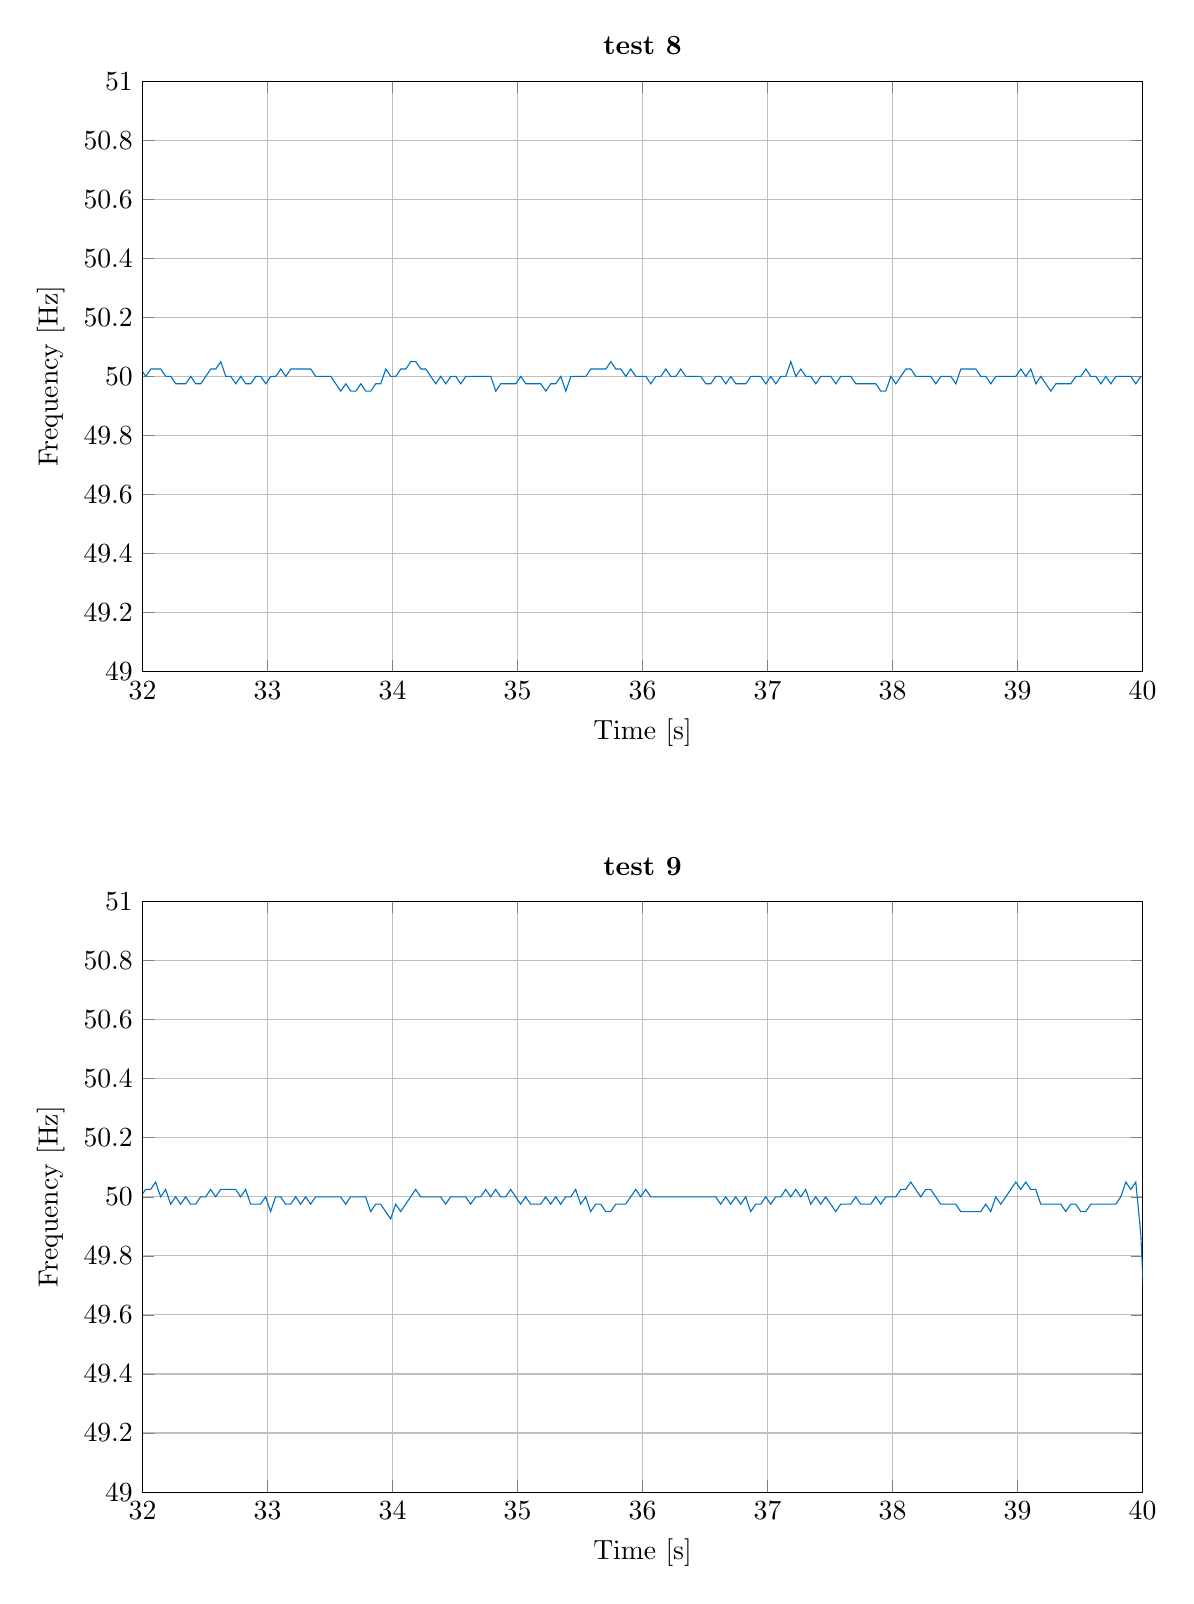
\begin{tikzpicture}

\begin{axis}[%
width=5in,
height=2.953in,
at={(1.142in,5.054in)},
scale only axis,
xmin=32,
xmax=40,
xlabel={Time [s]},
xmajorgrids,
ymin=49,
ymax=51,
ylabel={Frequency [Hz]},
ymajorgrids,
axis background/.style={fill=white},
title style={font=\bfseries},
title={test 8}
]
\addplot [color=mycolor1,solid,forget plot]
  table[row sep=crcr]{%
31.9859	50.0250125062577\\
32.02588	49.9999999999922\\
32.06588	50.0250125062532\\
32.10586	50.0250125062532\\
32.14584	50.0250125062532\\
32.18582	50.0000000000011\\
32.22582	50.0000000000011\\
32.26582	49.9750124937551\\
32.30584	49.9750124937551\\
32.34586	49.9750124937463\\
32.38588	50.0000000000011\\
32.42588	49.9750124937551\\
32.4659	49.9750124937551\\
32.50592	50.0000000000011\\
32.54592	50.0250125062532\\
32.5859	50.0250125062532\\
32.62588	50.0500500500492\\
32.66584	50.0000000000011\\
32.70584	50.0000000000011\\
32.74584	49.9750124937463\\
32.78586	50.0000000000011\\
32.82586	49.9750124937551\\
32.86588	49.9750124937551\\
32.9059	50.0000000000011\\
32.9459	50.0000000000011\\
32.9859	49.9750124937463\\
33.02592	50.0000000000011\\
33.06592	50.0000000000011\\
33.10592	50.0250125062532\\
33.1459	50.0000000000011\\
33.1859	50.0250125062532\\
33.22588	50.0250125062532\\
33.26586	50.0250125062532\\
33.30584	50.0250125062532\\
33.34582	50.0250125062532\\
33.3858	50.0000000000011\\
33.4258	50.0000000000011\\
33.4658	50.0000000000011\\
33.5058	49.9999999999922\\
33.5458	49.9750124937551\\
33.58582	49.9500499500529\\
33.62586	49.9750124937551\\
33.66588	49.950049950044\\
33.70592	49.9500499500529\\
33.74596	49.9750124937551\\
33.78598	49.950049950044\\
33.82602	49.9500499500529\\
33.86606	49.9750124937551\\
33.90608	49.9750124937551\\
33.9461	50.0250125062532\\
33.98608	49.9999999999922\\
34.02608	50.0000000000011\\
34.06608	50.0250125062532\\
34.10606	50.0250125062532\\
34.14604	50.0500500500492\\
34.186	50.0500500500581\\
34.22596	50.0250125062444\\
34.26594	50.0250125062532\\
34.30592	50.0000000000011\\
34.34592	49.9750124937551\\
34.38594	50.0000000000011\\
34.42594	49.9750124937551\\
34.46596	50.0000000000011\\
34.50596	50.0000000000011\\
34.54596	49.9750124937463\\
34.58598	50.0000000000011\\
34.62598	50.0000000000011\\
34.66598	50.0000000000011\\
34.70598	50.0000000000011\\
34.74598	50.0000000000011\\
34.78598	50.0000000000011\\
34.82598	49.950049950044\\
34.86602	49.9750124937551\\
34.90604	49.9750124937551\\
34.94606	49.9750124937551\\
34.98608	49.9750124937463\\
35.0261	50.0000000000011\\
35.0661	49.9750124937551\\
35.10612	49.9750124937551\\
35.14614	49.9750124937551\\
35.18616	49.9750124937463\\
35.22618	49.9500499500529\\
35.26622	49.9750124937551\\
35.30624	49.9750124937551\\
35.34626	49.9999999999922\\
35.38626	49.9500499500529\\
35.4263	50.0000000000011\\
35.4663	50.0000000000011\\
35.5063	50.0000000000011\\
35.5463	50.0000000000011\\
35.5863	50.0250125062532\\
35.62628	50.0250125062532\\
35.66626	50.0250125062532\\
35.70624	50.0250125062532\\
35.74622	50.0500500500492\\
35.78618	50.0250125062532\\
35.82616	50.0250125062532\\
35.86614	50.0000000000011\\
35.90614	50.0250125062532\\
35.94612	49.9999999999922\\
35.98612	50.0000000000011\\
36.02612	50.0000000000011\\
36.06612	49.9750124937551\\
36.10614	50.0000000000011\\
36.14614	50.0000000000011\\
36.18614	50.0250125062532\\
36.22612	50.0000000000011\\
36.26612	49.9999999999922\\
36.30612	50.0250125062532\\
36.3461	50.0000000000011\\
36.3861	50.0000000000011\\
36.4261	50.0000000000011\\
36.4661	50.0000000000011\\
36.5061	49.9750124937551\\
36.54612	49.9750124937463\\
36.58614	50.0000000000011\\
36.62614	50.0000000000011\\
36.66614	49.9750124937551\\
36.70616	50.0000000000011\\
36.74616	49.9750124937551\\
36.78618	49.9750124937463\\
36.8262	49.9750124937551\\
36.86622	50.0000000000011\\
36.90622	50.0000000000011\\
36.94622	50.0000000000011\\
36.98622	49.9750124937551\\
37.02624	50.0000000000011\\
37.06624	49.9750124937463\\
37.10626	50.0000000000011\\
37.14626	50.0000000000011\\
37.18626	50.0500500500492\\
37.22622	50.0000000000011\\
37.26622	50.0250125062532\\
37.3062	50.0000000000011\\
37.3462	50.0000000000011\\
37.3862	49.9750124937551\\
37.42622	49.9999999999922\\
37.46622	50.0000000000011\\
37.50622	50.0000000000011\\
37.54622	49.9750124937551\\
37.58624	50.0000000000011\\
37.62624	50.0000000000011\\
37.66624	50.0000000000011\\
37.70624	49.9750124937463\\
37.74626	49.9750124937551\\
37.78628	49.9750124937551\\
37.8263	49.9750124937551\\
37.86632	49.9750124937463\\
37.90634	49.9500499500529\\
37.94638	49.9500499500529\\
37.98642	50.0000000000011\\
38.02642	49.9750124937463\\
38.06644	50.0000000000011\\
38.10644	50.0250125062532\\
38.14642	50.0250125062532\\
38.1864	50.0000000000011\\
38.2264	50.0000000000011\\
38.2664	50.0000000000011\\
38.3064	50.0000000000011\\
38.3464	49.9750124937551\\
38.38642	50.0000000000011\\
38.42642	49.9999999999922\\
38.46642	50.0000000000011\\
38.50642	49.9750124937551\\
38.54644	50.0250125062532\\
38.58642	50.0250125062532\\
38.6264	50.0250125062532\\
38.66638	50.0250125062532\\
38.70636	50.0000000000011\\
38.74636	50.0000000000011\\
38.78636	49.9750124937551\\
38.82638	49.9999999999922\\
38.86638	50.0000000000011\\
38.90638	50.0000000000011\\
38.94638	50.0000000000011\\
38.98638	50.0000000000011\\
39.02638	50.0250125062532\\
39.06636	50.0000000000011\\
39.10636	50.0250125062532\\
39.14634	49.9750124937551\\
39.18636	49.9999999999922\\
39.22636	49.9750124937551\\
39.26638	49.9500499500529\\
39.30642	49.9750124937551\\
39.34644	49.9750124937463\\
39.38646	49.9750124937551\\
39.42648	49.9750124937551\\
39.4665	50.0000000000011\\
39.5065	50.0000000000011\\
39.5465	50.0250125062532\\
39.58648	50.0000000000011\\
39.62648	49.9999999999922\\
39.66648	49.9750124937551\\
39.7065	50.0000000000011\\
39.7465	49.9750124937551\\
39.78652	50.0000000000011\\
39.82652	50.0000000000011\\
39.86652	50.0000000000011\\
39.90652	49.9999999999922\\
39.94652	49.9750124937551\\
39.98654	50.0000000000011\\
40.02654	50.0000000000011\\
};
\end{axis}

\begin{axis}[%
width=5in,
height=2.953in,
at={(1.142in,0.952in)},
scale only axis,
xmin=32,
xmax=40,
xlabel={Time [s]},
xmajorgrids,
ymin=49,
ymax=51,
ylabel={Frequency [Hz]},
ymajorgrids,
axis background/.style={fill=white},
title style={font=\bfseries},
title={test 9 }
]
\addplot [color=mycolor1,solid,forget plot]
  table[row sep=crcr]{%
31.98468	50.0000000000011\\
32.02468	50.0250125062532\\
32.06466	50.0250125062532\\
32.10464	50.0500500500492\\
32.1446	50.0000000000011\\
32.1846	50.0250125062532\\
32.22458	49.9750124937551\\
32.2646	49.9999999999922\\
32.3046	49.9750124937551\\
32.34462	50.0000000000011\\
32.38462	49.9750124937551\\
32.42464	49.9750124937551\\
32.46466	50.0000000000011\\
32.50466	49.9999999999922\\
32.54466	50.0250125062532\\
32.58464	50.0000000000011\\
32.62464	50.0250125062532\\
32.66462	50.0250125062532\\
32.7046	50.0250125062532\\
32.74458	50.0250125062532\\
32.78456	50.0000000000011\\
32.82456	50.0250125062532\\
32.86454	49.9750124937551\\
32.90456	49.9750124937551\\
32.94458	49.9750124937463\\
32.9846	50.0000000000011\\
33.0246	49.9500499500529\\
33.06464	50.0000000000011\\
33.10464	50.0000000000011\\
33.14464	49.9750124937551\\
33.18466	49.9750124937463\\
33.22468	50.0000000000011\\
33.26468	49.9750124937551\\
33.3047	50.0000000000011\\
33.3447	49.9750124937551\\
33.38472	50.0000000000011\\
33.42472	49.9999999999922\\
33.46472	50.0000000000011\\
33.50472	50.0000000000011\\
33.54472	50.0000000000011\\
33.58472	50.0000000000011\\
33.62472	49.9750124937551\\
33.66474	50.0000000000011\\
33.70474	49.9999999999922\\
33.74474	50.0000000000011\\
33.78474	50.0000000000011\\
33.82474	49.9500499500529\\
33.86478	49.9750124937551\\
33.9048	49.9750124937463\\
33.94482	49.9500499500529\\
33.98486	49.9251123315066\\
34.02492	49.9750124937463\\
34.06494	49.9500499500529\\
34.10498	49.9750124937551\\
34.145	50.0000000000011\\
34.185	50.0250125062532\\
34.22498	50.0000000000011\\
34.26498	49.9999999999922\\
34.30498	50.0000000000011\\
34.34498	50.0000000000011\\
34.38498	50.0000000000011\\
34.42498	49.9750124937551\\
34.465	50.0000000000011\\
34.505	50.0000000000011\\
34.545	50.0000000000011\\
34.585	49.9999999999922\\
34.625	49.9750124937551\\
34.66502	50.0000000000011\\
34.70502	50.0000000000011\\
34.74502	50.0250125062532\\
34.785	50.0000000000011\\
34.825	50.0250125062532\\
34.86498	50.0000000000011\\
34.90498	50.0000000000011\\
34.94498	50.0250125062532\\
34.98496	49.9999999999922\\
35.02496	49.9750124937551\\
35.06498	50.0000000000011\\
35.10498	49.9750124937551\\
35.145	49.9750124937551\\
35.18502	49.9750124937463\\
35.22504	50.0000000000011\\
35.26504	49.9750124937551\\
35.30506	50.0000000000011\\
35.34506	49.9750124937551\\
35.38508	50.0000000000011\\
35.42508	49.9999999999922\\
35.46508	50.0250125062532\\
35.50506	49.9750124937551\\
35.54508	50.0000000000011\\
35.58508	49.9500499500529\\
35.62512	49.9750124937551\\
35.66514	49.9750124937463\\
35.70516	49.9500499500529\\
35.7452	49.9500499500529\\
35.78524	49.9750124937463\\
35.82526	49.9750124937551\\
35.86528	49.9750124937551\\
35.9053	50.0000000000011\\
35.9453	50.0250125062532\\
35.98528	50.0000000000011\\
36.02528	50.0250125062532\\
36.06526	50.0000000000011\\
36.10526	50.0000000000011\\
36.14526	49.9999999999922\\
36.18526	50.0000000000011\\
36.22526	50.0000000000011\\
36.26526	50.0000000000011\\
36.30526	50.0000000000011\\
36.34526	50.0000000000011\\
36.38526	50.0000000000011\\
36.42526	50.0000000000011\\
36.46526	49.9999999999922\\
36.50526	50.0000000000011\\
36.54526	50.0000000000011\\
36.58526	50.0000000000011\\
36.62526	49.9750124937551\\
36.66528	50.0000000000011\\
36.70528	49.9750124937463\\
36.7453	50.0000000000011\\
36.7853	49.9750124937551\\
36.82532	50.0000000000011\\
36.86532	49.9500499500529\\
36.90536	49.9750124937463\\
36.94538	49.9750124937551\\
36.9854	50.0000000000011\\
37.0254	49.9750124937551\\
37.06542	50.0000000000011\\
37.10542	50.0000000000011\\
37.14542	50.0250125062532\\
37.1854	50.0000000000011\\
37.2254	50.0250125062532\\
37.26538	49.9999999999922\\
37.30538	50.0250125062532\\
37.34536	49.9750124937551\\
37.38538	50.0000000000011\\
37.42538	49.9750124937551\\
37.4654	50.0000000000011\\
37.5054	49.9750124937463\\
37.54542	49.9500499500529\\
37.58546	49.9750124937551\\
37.62548	49.9750124937551\\
37.6655	49.9750124937463\\
37.70552	50.0000000000011\\
37.74552	49.9750124937551\\
37.78554	49.9750124937551\\
37.82556	49.9750124937551\\
37.86558	50.0000000000011\\
37.90558	49.9750124937463\\
37.9456	50.0000000000011\\
37.9856	50.0000000000011\\
38.0256	50.0000000000011\\
38.0656	50.0250125062532\\
38.10558	50.0250125062532\\
38.14556	50.0500500500492\\
38.18552	50.0250125062532\\
38.2255	50.0000000000011\\
38.2655	50.0250125062532\\
38.30548	50.0250125062532\\
38.34546	50.0000000000011\\
38.38546	49.9750124937551\\
38.42548	49.9750124937463\\
38.4655	49.9750124937551\\
38.50552	49.9750124937551\\
38.54554	49.9500499500529\\
38.58558	49.950049950044\\
38.62562	49.9500499500529\\
38.66566	49.9500499500529\\
38.7057	49.950049950044\\
38.74574	49.9750124937551\\
38.78576	49.9500499500529\\
38.8258	49.9999999999922\\
38.8658	49.9750124937551\\
38.90582	50.0000000000011\\
38.94582	50.0250125062532\\
38.9858	50.0500500500492\\
39.02576	50.0250125062532\\
39.06574	50.0500500500492\\
39.1057	50.0250125062532\\
39.14568	50.0250125062532\\
39.18566	49.9750124937551\\
39.22568	49.9750124937551\\
39.2657	49.9750124937551\\
39.30572	49.9750124937463\\
39.34574	49.9750124937551\\
39.38576	49.9500499500529\\
39.4258	49.9750124937551\\
39.46582	49.9750124937463\\
39.50584	49.9500499500529\\
39.54588	49.9500499500529\\
39.58592	49.9750124937463\\
39.62594	49.9750124937551\\
39.66596	49.9750124937551\\
39.70598	49.9750124937551\\
39.746	49.9750124937551\\
39.78602	49.9750124937463\\
39.82604	50.0000000000011\\
39.86604	50.0500500500492\\
39.906	50.0250125062532\\
39.94598	50.0500500500492\\
39.98594	49.875311720704\\
40.02604	49.5049504950517\\
};
\end{axis}
\end{tikzpicture}%
\caption{Steady state frequency output of the genset at 40 kW load.}
\label{fig:test8-9steadyfrequency40kw}
\end{figure}

\begin{figure}[H]
\centering
% This file was created by matlab2tikz.
%
%The latest updates can be retrieved from
%  http://www.mathworks.com/matlabcentral/fileexchange/22022-matlab2tikz-matlab2tikz
%where you can also make suggestions and rate matlab2tikz.
%
\definecolor{mycolor1}{rgb}{0.00000,0.44700,0.74100}%
%
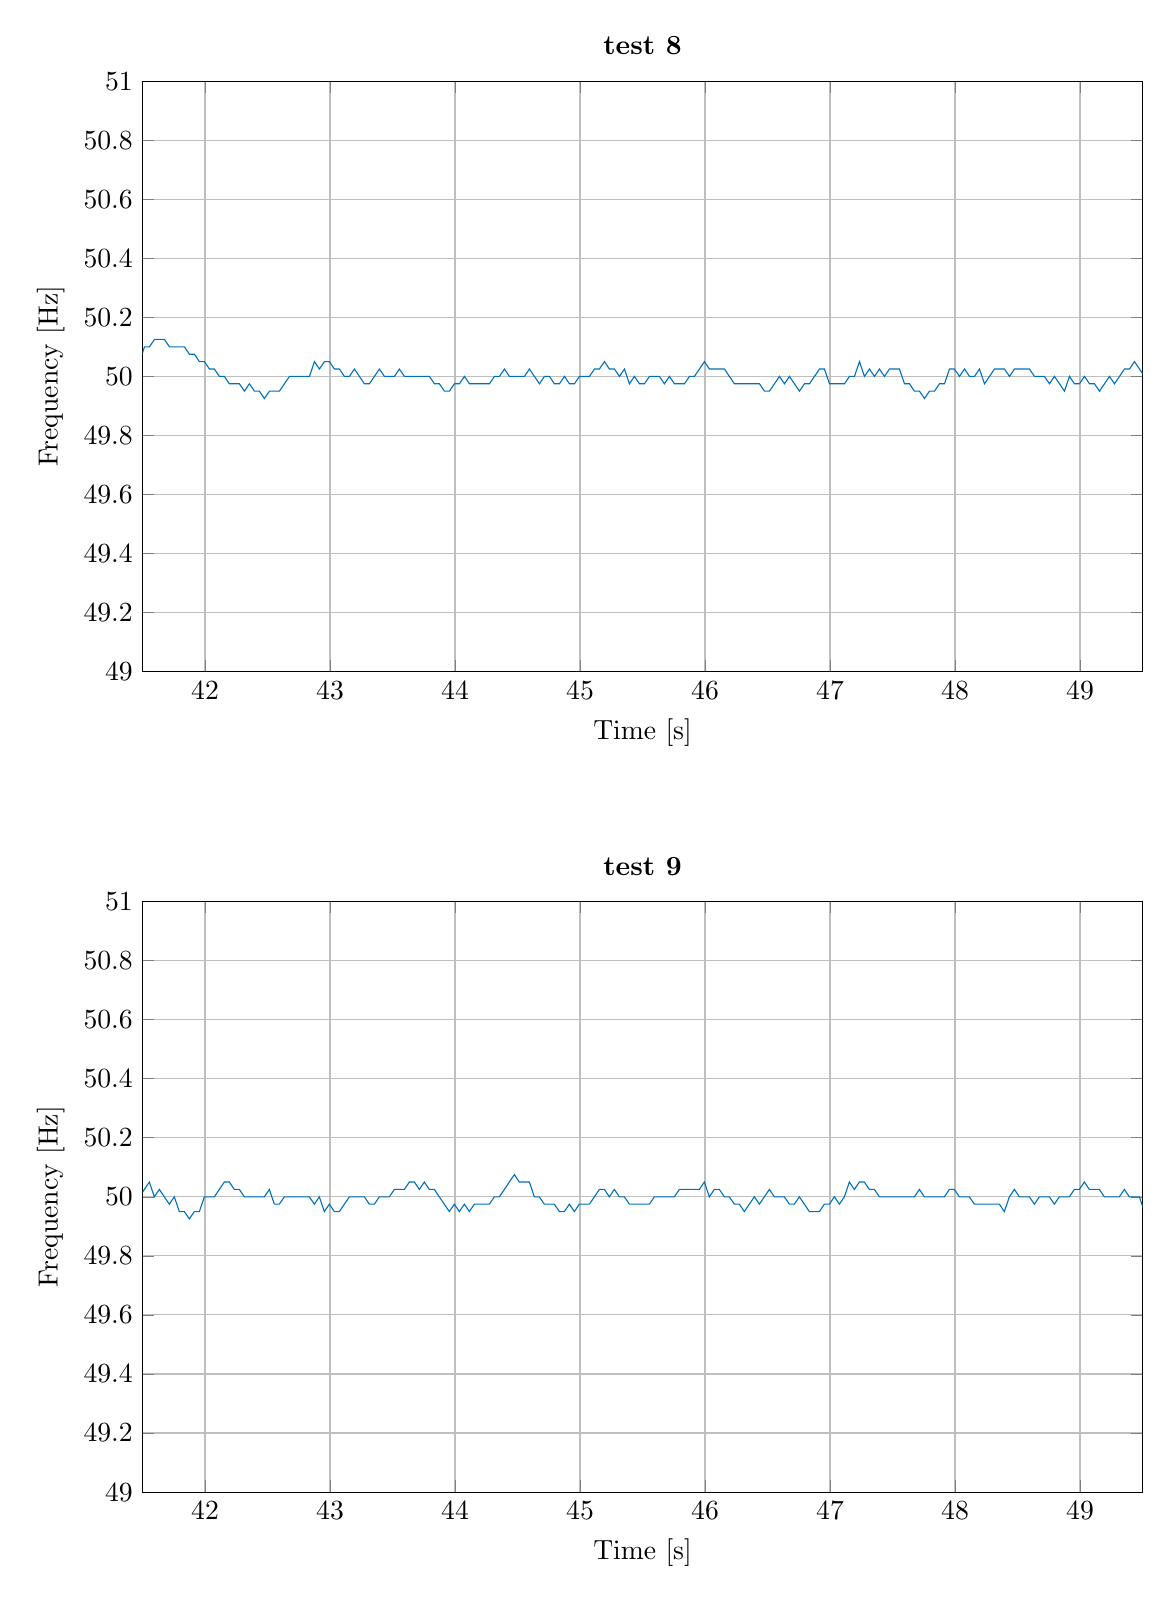
\begin{tikzpicture}

\begin{axis}[%
width=5in,
height=2.953in,
at={(1.142in,5.054in)},
scale only axis,
xmin=41.5,
xmax=49.5,
xlabel={Time [s]},
xmajorgrids,
ymin=49,
ymax=51,
ylabel={Frequency [Hz]},
ymajorgrids,
axis background/.style={fill=white},
title style={font=\bfseries},
title={test 8}
]
\addplot [color=mycolor1,solid,forget plot]
  table[row sep=crcr]{%
41.4758	50.0500500500581\\
41.51576	50.1002004007989\\
41.55568	50.1002004007989\\
41.5956	50.1253132832133\\
41.6355	50.1253132832043\\
41.6754	50.1253132832043\\
41.7153	50.1002004008078\\
41.75522	50.1002004007989\\
41.79514	50.1002004007989\\
41.83506	50.1002004008078\\
41.87498	50.0751126690017\\
41.91492	50.0751126690017\\
41.95486	50.0500500500492\\
41.99482	50.0500500500492\\
42.03478	50.0250125062532\\
42.07476	50.0250125062532\\
42.11474	50.0000000000011\\
42.15474	50.0000000000011\\
42.19474	49.9750124937551\\
42.23476	49.9750124937463\\
42.27478	49.9750124937551\\
42.3148	49.9500499500529\\
42.35484	49.9750124937551\\
42.39486	49.950049950044\\
42.4349	49.9500499500529\\
42.47494	49.9251123315066\\
42.515	49.950049950044\\
42.55504	49.9500499500529\\
42.59508	49.9500499500529\\
42.63512	49.9750124937463\\
42.67514	50.0000000000011\\
42.71514	50.0000000000011\\
42.75514	50.0000000000011\\
42.79514	50.0000000000011\\
42.83514	50.0000000000011\\
42.87514	50.0500500500492\\
42.9151	50.0250125062532\\
42.95508	50.0500500500492\\
42.99504	50.0500500500492\\
43.035	50.0250125062532\\
43.07498	50.0250125062532\\
43.11496	50.0000000000011\\
43.15496	50.0000000000011\\
43.19496	50.0250125062532\\
43.23494	50.0000000000011\\
43.27494	49.9750124937463\\
43.31496	49.9750124937551\\
43.35498	50.0000000000011\\
43.39498	50.0250125062532\\
43.43496	50.0000000000011\\
43.47496	50.0000000000011\\
43.51496	50.0000000000011\\
43.55496	50.0250125062532\\
43.59494	50.0000000000011\\
43.63494	49.9999999999922\\
43.67494	50.0000000000011\\
43.71494	50.0000000000011\\
43.75494	50.0000000000011\\
43.79494	50.0000000000011\\
43.83494	49.9750124937551\\
43.87496	49.9750124937551\\
43.91498	49.950049950044\\
43.95502	49.9500499500529\\
43.99506	49.9750124937551\\
44.03508	49.9750124937463\\
44.0751	50.0000000000011\\
44.1151	49.9750124937551\\
44.15512	49.9750124937551\\
44.19514	49.9750124937551\\
44.23516	49.9750124937463\\
44.27518	49.9750124937551\\
44.3152	50.0000000000011\\
44.3552	50.0000000000011\\
44.3952	50.0250125062532\\
44.43518	50.0000000000011\\
44.47518	50.0000000000011\\
44.51518	50.0000000000011\\
44.55518	49.9999999999922\\
44.59518	50.0250125062532\\
44.63516	50.0000000000011\\
44.67516	49.9750124937551\\
44.71518	50.0000000000011\\
44.75518	50.0000000000011\\
44.79518	49.9750124937551\\
44.8352	49.9750124937463\\
44.87522	50.0000000000011\\
44.91522	49.9750124937551\\
44.95524	49.9750124937551\\
44.99526	50.0000000000011\\
45.03526	50.0000000000011\\
45.07526	49.9999999999922\\
45.11526	50.0250125062532\\
45.15524	50.0250125062532\\
45.19522	50.0500500500581\\
45.23518	50.0250125062532\\
45.27516	50.0250125062444\\
45.31514	50.0000000000011\\
45.35514	50.0250125062532\\
45.39512	49.9750124937551\\
45.43514	50.0000000000011\\
45.47514	49.9750124937551\\
45.51516	49.9750124937551\\
45.55518	49.9999999999922\\
45.59518	50.0000000000011\\
45.63518	50.0000000000011\\
45.67518	49.9750124937551\\
45.7152	50.0000000000011\\
45.7552	49.9750124937551\\
45.79522	49.9750124937463\\
45.83524	49.9750124937551\\
45.87526	50.0000000000011\\
45.91526	50.0000000000011\\
45.95526	50.0250125062532\\
45.99524	50.0500500500492\\
46.0352	50.0250125062532\\
46.07518	50.0250125062532\\
46.11516	50.0250125062532\\
46.15514	50.0250125062532\\
46.19512	50.0000000000011\\
46.23512	49.9750124937551\\
46.27514	49.9750124937463\\
46.31516	49.9750124937551\\
46.35518	49.9750124937551\\
46.3952	49.9750124937551\\
46.43522	49.9750124937463\\
46.47524	49.9500499500529\\
46.51528	49.9500499500529\\
46.55532	49.9750124937551\\
46.59534	49.9999999999922\\
46.63534	49.9750124937551\\
46.67536	50.0000000000011\\
46.71536	49.9750124937551\\
46.75538	49.9500499500529\\
46.79542	49.9750124937463\\
46.83544	49.9750124937551\\
46.87546	50.0000000000011\\
46.91546	50.0250125062532\\
46.95544	50.0250125062532\\
46.99542	49.9750124937551\\
47.03544	49.9750124937551\\
47.07546	49.9750124937463\\
47.11548	49.9750124937551\\
47.1555	50.0000000000011\\
47.1955	50.0000000000011\\
47.2355	50.0500500500492\\
47.27546	50.0000000000011\\
47.31546	50.0250125062532\\
47.35544	50.0000000000011\\
47.39544	50.0250125062532\\
47.43542	50.0000000000011\\
47.47542	50.0250125062532\\
47.5154	50.0250125062532\\
47.55538	50.0250125062532\\
47.59536	49.9750124937463\\
47.63538	49.9750124937551\\
47.6754	49.9500499500529\\
47.71544	49.950049950044\\
47.75548	49.9251123315066\\
47.79554	49.9500499500529\\
47.83558	49.950049950044\\
47.87562	49.9750124937551\\
47.91564	49.9750124937551\\
47.95566	50.0250125062532\\
47.99564	50.0250125062532\\
48.03562	50.0000000000011\\
48.07562	50.0250125062532\\
48.1156	50.0000000000011\\
48.1556	49.9999999999922\\
48.1956	50.0250125062532\\
48.23558	49.9750124937551\\
48.2756	50.0000000000011\\
48.3156	50.0250125062532\\
48.35558	50.0250125062532\\
48.39556	50.0250125062532\\
48.43554	50.0000000000011\\
48.47554	50.0250125062532\\
48.51552	50.0250125062532\\
48.5555	50.0250125062532\\
48.59548	50.0250125062532\\
48.63546	50.0000000000011\\
48.67546	50.0000000000011\\
48.71546	50.0000000000011\\
48.75546	49.9750124937463\\
48.79548	50.0000000000011\\
48.83548	49.9750124937551\\
48.8755	49.9500499500529\\
48.91554	49.9999999999922\\
48.95554	49.9750124937551\\
48.99556	49.9750124937551\\
49.03558	50.0000000000011\\
49.07558	49.9750124937551\\
49.1156	49.9750124937463\\
49.15562	49.9500499500529\\
49.19566	49.9750124937551\\
49.23568	50.0000000000011\\
49.27568	49.9750124937551\\
49.3157	49.9999999999922\\
49.3557	50.0250125062532\\
49.39568	50.0250125062532\\
49.43566	50.0500500500581\\
49.47562	50.0250125062444\\
49.5156	50.0000000000011\\
};
\end{axis}

\begin{axis}[%
width=5in,
height=2.953in,
at={(1.142in,0.952in)},
scale only axis,
xmin=41.5,
xmax=49.5,
xlabel={Time [s]},
xmajorgrids,
ymin=49,
ymax=51,
ylabel={Frequency [Hz]},
ymajorgrids,
axis background/.style={fill=white},
title style={font=\bfseries},
title={test 9}
]
\addplot [color=mycolor1,solid,forget plot]
  table[row sep=crcr]{%
41.47428	49.9999999999922\\
41.51428	50.0250125062532\\
41.55426	50.0500500500581\\
41.59422	49.9999999999922\\
41.63422	50.0250125062532\\
41.6742	50.0000000000011\\
41.7142	49.9750124937551\\
41.75422	50.0000000000011\\
41.79422	49.9500499500529\\
41.83426	49.950049950044\\
41.8743	49.9251123315066\\
41.91436	49.950049950044\\
41.9544	49.9500499500529\\
41.99444	50.0000000000011\\
42.03444	50.0000000000011\\
42.07444	50.0000000000011\\
42.11444	50.0250125062532\\
42.15442	50.0500500500492\\
42.19438	50.0500500500492\\
42.23434	50.0250125062532\\
42.27432	50.0250125062532\\
42.3143	50.0000000000011\\
42.3543	50.0000000000011\\
42.3943	50.0000000000011\\
42.4343	49.9999999999922\\
42.4743	50.0000000000011\\
42.5143	50.0250125062532\\
42.55428	49.9750124937551\\
42.5943	49.9750124937551\\
42.63432	50.0000000000011\\
42.67432	50.0000000000011\\
42.71432	50.0000000000011\\
42.75432	49.9999999999922\\
42.79432	50.0000000000011\\
42.83432	50.0000000000011\\
42.87432	49.9750124937551\\
42.91434	50.0000000000011\\
42.95434	49.950049950044\\
42.99438	49.9750124937551\\
43.0344	49.9500499500529\\
43.07444	49.9500499500529\\
43.11448	49.9750124937463\\
43.1545	50.0000000000011\\
43.1945	50.0000000000011\\
43.2345	50.0000000000011\\
43.2745	50.0000000000011\\
43.3145	49.9750124937551\\
43.35452	49.9750124937463\\
43.39454	50.0000000000011\\
43.43454	50.0000000000011\\
43.47454	50.0000000000011\\
43.51454	50.0250125062532\\
43.55452	50.0250125062532\\
43.5945	50.0250125062532\\
43.63448	50.0500500500492\\
43.67444	50.0500500500492\\
43.7144	50.0250125062532\\
43.75438	50.0500500500492\\
43.79434	50.0250125062532\\
43.83432	50.0250125062532\\
43.8743	50.0000000000011\\
43.9143	49.9750124937551\\
43.95432	49.9500499500529\\
43.99436	49.9750124937463\\
44.03438	49.9500499500529\\
44.07442	49.9750124937551\\
44.11444	49.950049950044\\
44.15448	49.9750124937551\\
44.1945	49.9750124937551\\
44.23452	49.9750124937551\\
44.27454	49.9750124937551\\
44.31456	49.9999999999922\\
44.35456	50.0000000000011\\
44.39456	50.0250125062532\\
44.43454	50.0500500500492\\
44.4745	50.0751126690106\\
44.51444	50.0500500500492\\
44.5544	50.0500500500492\\
44.59436	50.0500500500492\\
44.63432	50.0000000000011\\
44.67432	50.0000000000011\\
44.71432	49.9750124937463\\
44.75434	49.9750124937551\\
44.79436	49.9750124937551\\
44.83438	49.9500499500529\\
44.87442	49.950049950044\\
44.91446	49.9750124937551\\
44.95448	49.9500499500529\\
44.99452	49.9750124937551\\
45.03454	49.9750124937463\\
45.07456	49.9750124937551\\
45.11458	50.0000000000011\\
45.15458	50.0250125062532\\
45.19456	50.0250125062532\\
45.23454	50.0000000000011\\
45.27454	50.0250125062532\\
45.31452	50.0000000000011\\
45.35452	50.0000000000011\\
45.39452	49.9750124937463\\
45.43454	49.9750124937551\\
45.47456	49.9750124937551\\
45.51458	49.9750124937551\\
45.5546	49.9750124937463\\
45.59462	50.0000000000011\\
45.63462	50.0000000000011\\
45.67462	50.0000000000011\\
45.71462	50.0000000000011\\
45.75462	50.0000000000011\\
45.79462	50.0250125062532\\
45.8346	50.0250125062532\\
45.87458	50.0250125062532\\
45.91456	50.0250125062532\\
45.95454	50.0250125062532\\
45.99452	50.0500500500492\\
46.03448	50.0000000000011\\
46.07448	50.0250125062532\\
46.11446	50.0250125062532\\
46.15444	50.0000000000011\\
46.19444	49.9999999999922\\
46.23444	49.9750124937551\\
46.27446	49.9750124937551\\
46.31448	49.9500499500529\\
46.35452	49.9750124937463\\
46.39454	50.0000000000011\\
46.43454	49.9750124937551\\
46.47456	50.0000000000011\\
46.51456	50.0250125062532\\
46.55454	50.0000000000011\\
46.59454	50.0000000000011\\
46.63454	50.0000000000011\\
46.67454	49.9750124937463\\
46.71456	49.9750124937551\\
46.75458	50.0000000000011\\
46.79458	49.9750124937551\\
46.8346	49.950049950044\\
46.87464	49.9500499500529\\
46.91468	49.9500499500529\\
46.95472	49.9750124937551\\
46.99474	49.9750124937463\\
47.03476	50.0000000000011\\
47.07476	49.9750124937551\\
47.11478	50.0000000000011\\
47.15478	50.0500500500492\\
47.19474	50.0250125062532\\
47.23472	50.0500500500492\\
47.27468	50.0500500500492\\
47.31464	50.0250125062532\\
47.35462	50.0250125062532\\
47.3946	50.0000000000011\\
47.4346	50.0000000000011\\
47.4746	50.0000000000011\\
47.5146	50.0000000000011\\
47.5546	50.0000000000011\\
47.5946	49.9999999999922\\
47.6346	50.0000000000011\\
47.6746	50.0000000000011\\
47.7146	50.0250125062532\\
47.75458	50.0000000000011\\
47.79458	50.0000000000011\\
47.83458	50.0000000000011\\
47.87458	50.0000000000011\\
47.91458	50.0000000000011\\
47.95458	50.0250125062532\\
47.99456	50.0250125062532\\
48.03454	49.9999999999922\\
48.07454	50.0000000000011\\
48.11454	50.0000000000011\\
48.15454	49.9750124937551\\
48.19456	49.9750124937551\\
48.23458	49.9750124937551\\
48.2746	49.9750124937463\\
48.31462	49.9750124937551\\
48.35464	49.9750124937551\\
48.39466	49.9500499500529\\
48.4347	49.9999999999922\\
48.4747	50.0250125062532\\
48.51468	50.0000000000011\\
48.55468	50.0000000000011\\
48.59468	50.0000000000011\\
48.63468	49.9750124937551\\
48.6747	50.0000000000011\\
48.7147	50.0000000000011\\
48.7547	49.9999999999922\\
48.7947	49.9750124937551\\
48.83472	50.0000000000011\\
48.87472	50.0000000000011\\
48.91472	50.0000000000011\\
48.95472	50.0250125062532\\
48.9947	50.0250125062532\\
49.03468	50.0500500500492\\
49.07464	50.0250125062532\\
49.11462	50.0250125062532\\
49.1546	50.0250125062532\\
49.19458	50.0000000000011\\
49.23458	50.0000000000011\\
49.27458	50.0000000000011\\
49.31458	49.9999999999922\\
49.35458	50.0250125062532\\
49.39456	50.0000000000011\\
49.43456	50.0000000000011\\
49.47456	50.0000000000011\\
49.51456	49.9500499500529\\
};
\end{axis}
\end{tikzpicture}%
\caption{Steady state frequency output of the genset at 50 kW load.}
\label{fig:test8-9steadyfrequency50kw}
\end{figure}

% \subsubsection*{Power}
% \begin{figure}[H]
% \centering
% % This file was created by matlab2tikz.
%
%The latest updates can be retrieved from
%  http://www.mathworks.com/matlabcentral/fileexchange/22022-matlab2tikz-matlab2tikz
%where you can also make suggestions and rate matlab2tikz.
%
\definecolor{mycolor1}{rgb}{0.00000,0.44700,0.74100}%
%
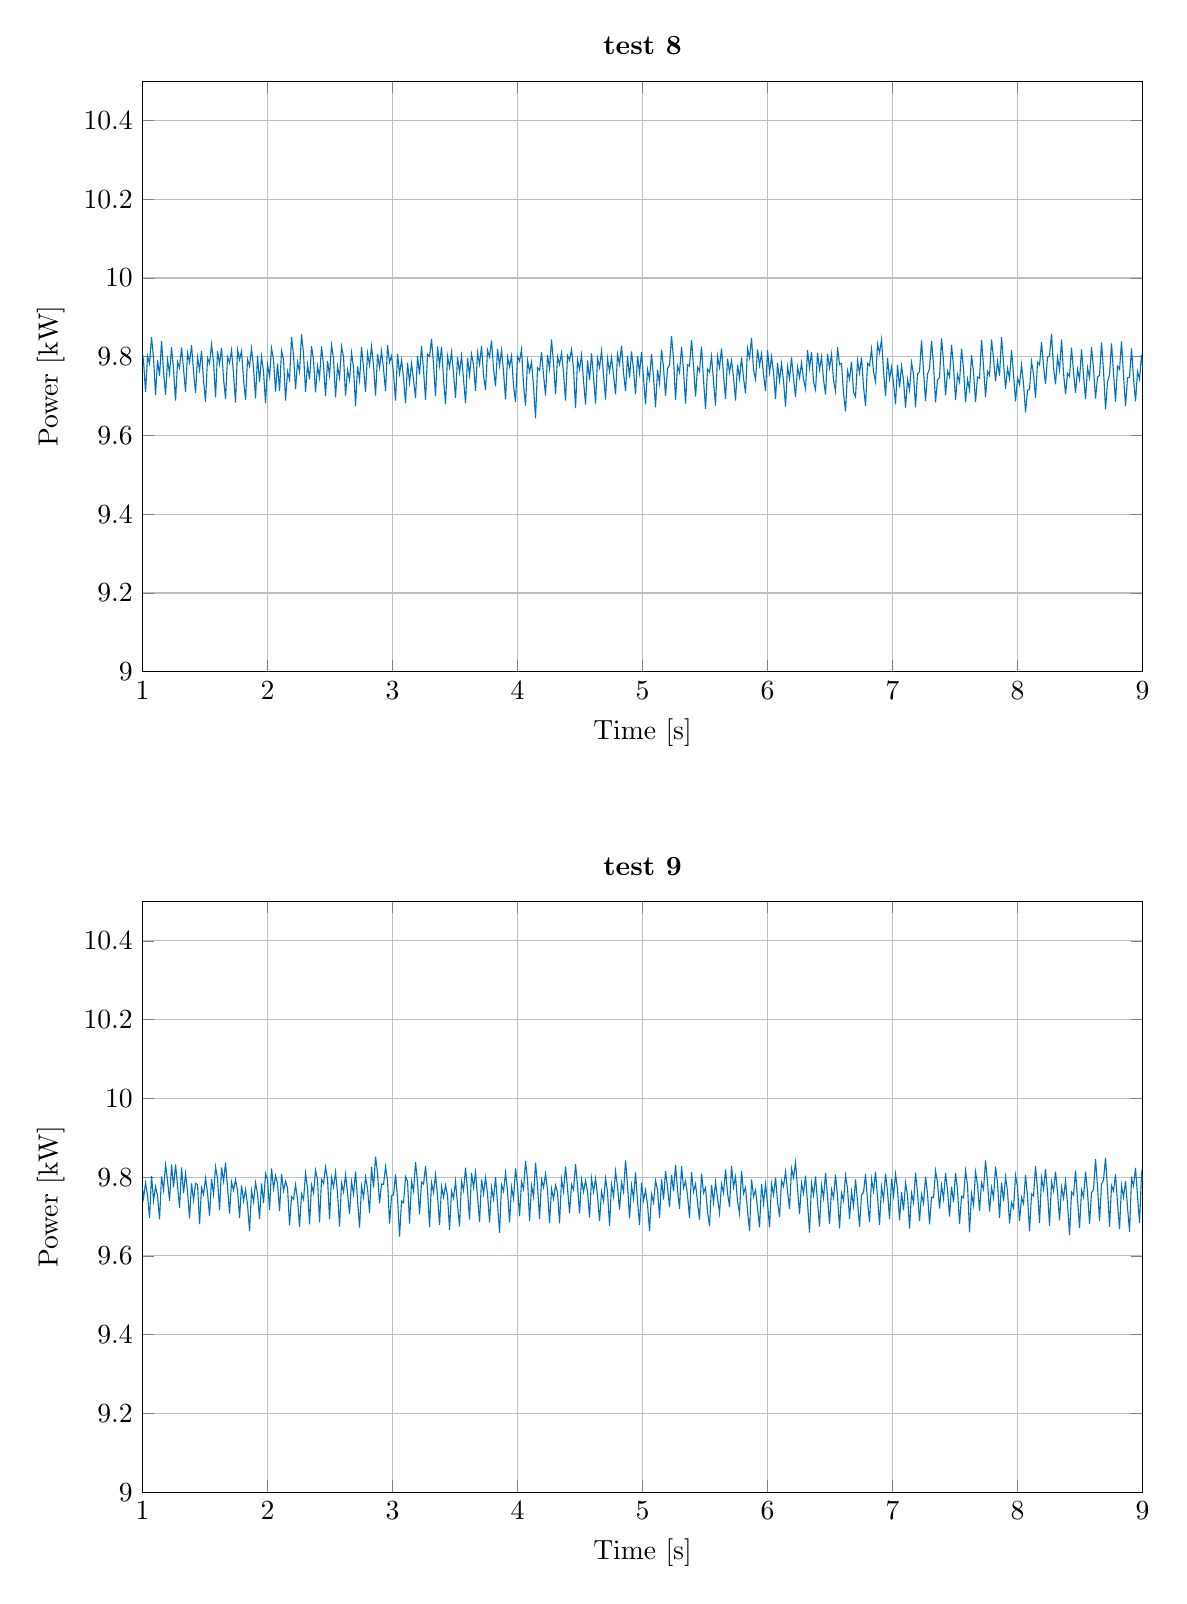
\begin{tikzpicture}

\begin{axis}[%
width=5in,
height=2.953in,
at={(1.142in,5.054in)},
scale only axis,
xmin=1,
xmax=9,
xlabel={Time [s]},
xmajorgrids,
ymin=9,
ymax=10.5,
ylabel={Power [kW]},
ymajorgrids,
axis background/.style={fill=white},
title style={font=\bfseries},
title={test 8}
]
\addplot [color=mycolor1,solid,forget plot]
  table[row sep=crcr]{%
0.992	9.82254302306233\\
1.008	9.78939277502938\\
1.024	9.71000208111662\\
1.04	9.80167259398623\\
1.056	9.7821073437088\\
1.072	9.84995152948031\\
1.088	9.79652131487928\\
1.104	9.7027657528374\\
1.12	9.79152442215694\\
1.136	9.75161468517418\\
1.152	9.8395035812992\\
1.168	9.76238919467365\\
1.184	9.70329614435497\\
1.2	9.79170983676165\\
1.216	9.75739544644562\\
1.232	9.8242151324909\\
1.248	9.76710640650664\\
1.264	9.68851332106347\\
1.28	9.78697878108676\\
1.296	9.77143910786893\\
1.312	9.82363711662156\\
1.328	9.76850704579906\\
1.344	9.71046875968203\\
1.36	9.80942769278896\\
1.376	9.78568868690533\\
1.392	9.82911585960516\\
1.408	9.76165178881501\\
1.424	9.70753066876593\\
1.44	9.79805186742755\\
1.456	9.76643406487604\\
1.472	9.81442456592497\\
1.488	9.73961660358693\\
1.504	9.68572108964297\\
1.52	9.79677130757456\\
1.536	9.78313874872454\\
1.552	9.83128169680672\\
1.568	9.78612073863349\\
1.584	9.69681212275362\\
1.6	9.81376664850239\\
1.616	9.78101755359582\\
1.632	9.82236034712568\\
1.648	9.74430483328607\\
1.664	9.69255045160363\\
1.68	9.79923139516197\\
1.696	9.78461599673483\\
1.712	9.81685240176827\\
1.728	9.75610600555322\\
1.744	9.68348686042403\\
1.76	9.81797863944677\\
1.776	9.79231457937574\\
1.792	9.81431513736696\\
1.808	9.74202853541923\\
1.824	9.69056272191575\\
1.84	9.79330969315986\\
1.856	9.77612768591282\\
1.872	9.82109292529563\\
1.888	9.77071969962261\\
1.904	9.69448526245878\\
1.92	9.80256521428901\\
1.936	9.73557657861913\\
1.952	9.80041075603538\\
1.968	9.76108450577979\\
1.984	9.68158541475999\\
2	9.77985976207856\\
2.016	9.75000760094089\\
2.032	9.82156250439172\\
2.048	9.79192905383481\\
2.064	9.71112709473945\\
2.08	9.78265965777364\\
2.096	9.71295620591759\\
2.112	9.81537983619642\\
2.128	9.7923624022294\\
2.144	9.68849873317481\\
2.16	9.76237018314975\\
2.176	9.74207358611414\\
2.192	9.85031211882443\\
2.208	9.80231862507264\\
2.224	9.71792675931678\\
2.24	9.78590051266873\\
2.256	9.7619206168263\\
2.272	9.85695343382533\\
2.288	9.80765004946975\\
2.304	9.71092975509773\\
2.32	9.78000438493982\\
2.336	9.74228805965951\\
2.352	9.82662109325454\\
2.368	9.79059247717394\\
2.384	9.70969223608576\\
2.4	9.77653861803379\\
2.416	9.74661779962059\\
2.432	9.82632855488625\\
2.448	9.77700342853195\\
2.464	9.70023333500084\\
2.48	9.78906536492014\\
2.496	9.75305200128796\\
2.512	9.82972021319082\\
2.528	9.79551372389316\\
2.544	9.69683646292411\\
2.56	9.77520602732169\\
2.576	9.7465627913762\\
2.592	9.82568826590802\\
2.608	9.7992950007759\\
2.624	9.70106894843558\\
2.64	9.76595437388665\\
2.656	9.7406119309273\\
2.672	9.81020866944342\\
2.688	9.77171851739345\\
2.704	9.67476172527606\\
2.72	9.77569241846723\\
2.736	9.74020793630512\\
2.752	9.82411375213276\\
2.768	9.77054218510168\\
2.784	9.7103193173811\\
2.8	9.80840006684069\\
2.816	9.7790545907307\\
2.832	9.82637138832808\\
2.848	9.77724473084057\\
2.864	9.70111488771154\\
2.88	9.80643308415018\\
2.896	9.77234533693603\\
2.912	9.8146079408256\\
2.928	9.76882991393454\\
2.944	9.71282515266007\\
2.96	9.82938492888433\\
2.976	9.78632563211893\\
2.992	9.80200680461029\\
3.008	9.75740984195725\\
3.024	9.68834992261044\\
3.04	9.80741541321671\\
3.056	9.75688390846573\\
3.072	9.79177253273646\\
3.088	9.74536630164004\\
3.104	9.68193342290925\\
3.12	9.78463698881434\\
3.136	9.73436360628003\\
3.152	9.78302609733207\\
3.168	9.7410932947323\\
3.184	9.6952888304763\\
3.2	9.80220848410441\\
3.216	9.75435770388276\\
3.232	9.82721503138204\\
3.248	9.76628204896475\\
3.264	9.690655540739\\
3.28	9.80605556143578\\
3.296	9.80083131850831\\
3.312	9.84526048200756\\
3.328	9.77879348136343\\
3.344	9.70008482667929\\
3.36	9.82642078239947\\
3.376	9.77738423031076\\
3.392	9.82508491650095\\
3.408	9.74327184502647\\
3.424	9.67925309527153\\
3.44	9.80146247054961\\
3.456	9.77319058303399\\
3.472	9.81205848267756\\
3.488	9.7566813911602\\
3.504	9.69548603796856\\
3.52	9.79855365917004\\
3.536	9.76036216421865\\
3.552	9.80189389522019\\
3.568	9.74251282176624\\
3.584	9.68197954569568\\
3.6	9.7969127656754\\
3.616	9.75308157128876\\
3.632	9.8064860720332\\
3.648	9.77875597695449\\
3.664	9.71327596447374\\
3.68	9.81011953248196\\
3.696	9.78048372493744\\
3.712	9.82664313896267\\
3.728	9.75265690503257\\
3.744	9.71516714697245\\
3.76	9.81651797446624\\
3.776	9.79960198647121\\
3.792	9.84106269229566\\
3.808	9.76956086467702\\
3.824	9.72510598771532\\
3.84	9.81940050473573\\
3.856	9.77725467787175\\
3.872	9.81672185499601\\
3.888	9.76122134624576\\
3.904	9.69144022612012\\
3.92	9.79896596095587\\
3.936	9.77451529228301\\
3.952	9.80232035909631\\
3.968	9.7259302217713\\
3.984	9.68511632090091\\
4	9.80052011297973\\
4.016	9.7887693543718\\
4.032	9.81929483419097\\
4.048	9.72840732593049\\
4.064	9.67560817800935\\
4.08	9.79064611123195\\
4.096	9.76212072030235\\
4.112	9.7866501904994\\
4.128	9.72426213688009\\
4.144	9.64354841727051\\
4.16	9.77193631947375\\
4.176	9.76515496575586\\
4.192	9.81145761922846\\
4.208	9.75349530728531\\
4.224	9.70132510349215\\
4.24	9.80404640043288\\
4.256	9.76941646602596\\
4.272	9.84369677136705\\
4.288	9.78347862167858\\
4.304	9.70425492671778\\
4.32	9.79998708390627\\
4.336	9.78020603272278\\
4.352	9.80982083124049\\
4.368	9.75817185077296\\
4.384	9.6887732630391\\
4.4	9.80291081987669\\
4.416	9.79095793049135\\
4.432	9.81825946268903\\
4.448	9.76828336223027\\
4.464	9.66921649558806\\
4.48	9.7925440210439\\
4.496	9.76765941687199\\
4.512	9.80439564125334\\
4.528	9.73928538394185\\
4.544	9.67848348025197\\
4.56	9.79038901883677\\
4.576	9.74079559635201\\
4.592	9.80809234668353\\
4.608	9.74881494823721\\
4.624	9.68073946086242\\
4.64	9.79603405279541\\
4.656	9.77277798888705\\
4.672	9.81499315279527\\
4.688	9.75366502794014\\
4.704	9.69127182823601\\
4.72	9.79450797528226\\
4.736	9.76231665516159\\
4.752	9.7984346605633\\
4.768	9.75363103646665\\
4.784	9.70430019834568\\
4.8	9.80615882889224\\
4.816	9.78061729243072\\
4.832	9.82827211751004\\
4.848	9.75938592778989\\
4.864	9.71245852701746\\
4.88	9.80190451859849\\
4.896	9.7469261957526\\
4.912	9.81350092422272\\
4.928	9.76629746754966\\
4.944	9.70428195043099\\
4.96	9.80222466464911\\
4.976	9.75899273608029\\
4.992	9.81127590756678\\
5.008	9.74449972089937\\
5.024	9.67908029635132\\
5.04	9.76778575885026\\
5.056	9.74320981886255\\
5.072	9.80653430798869\\
5.088	9.74653931568599\\
5.104	9.6713618318613\\
5.12	9.76669056705391\\
5.136	9.73219254851773\\
5.152	9.81804561154221\\
5.168	9.77250121672183\\
5.184	9.70037081330083\\
5.2	9.76973235178209\\
5.216	9.7797163680518\\
5.232	9.85203395482931\\
5.248	9.79392002967617\\
5.264	9.6895634223441\\
5.28	9.77691945863985\\
5.296	9.75978995922362\\
5.312	9.82518884964704\\
5.328	9.76445754447953\\
5.344	9.68090151034198\\
5.36	9.77991352907235\\
5.376	9.77638906193726\\
5.392	9.84294242645283\\
5.408	9.77479387101572\\
5.424	9.69879340917481\\
5.44	9.77328736182207\\
5.456	9.76310949074869\\
5.472	9.82570029841911\\
5.488	9.73997544192055\\
5.504	9.66755398658826\\
5.52	9.76872311569184\\
5.536	9.76043962340791\\
5.552	9.80110319792727\\
5.568	9.73669414036534\\
5.584	9.67616617620101\\
5.6	9.80123843089499\\
5.616	9.77322129153768\\
5.632	9.82091493586857\\
5.648	9.75312365516402\\
5.664	9.69289743809424\\
5.68	9.79509040127161\\
5.696	9.7604546006725\\
5.712	9.79012769481976\\
5.728	9.74657429140615\\
5.744	9.68873609629255\\
5.76	9.77971320293428\\
5.776	9.74380981457722\\
5.792	9.79840743330833\\
5.808	9.74559467559975\\
5.824	9.70713939635414\\
5.84	9.82127514890113\\
5.856	9.797146264514\\
5.872	9.84691758751472\\
5.888	9.76632469934486\\
5.904	9.74228195057239\\
5.92	9.81851866813034\\
5.936	9.77806170892652\\
5.952	9.80785323146045\\
5.968	9.7542222749021\\
5.984	9.71366565561235\\
6	9.81672946240342\\
6.016	9.76036929778663\\
6.032	9.80007410725964\\
6.048	9.75949610995725\\
6.064	9.69257884515835\\
6.08	9.78343671683136\\
6.096	9.73881307235757\\
6.112	9.78261056044925\\
6.128	9.73818195184761\\
6.144	9.67327661579843\\
6.16	9.77425623950975\\
6.176	9.74391500203547\\
6.192	9.79799470687659\\
6.208	9.74550322869018\\
6.224	9.69839848234612\\
6.24	9.77387623998187\\
6.256	9.74714991951616\\
6.272	9.78455603496245\\
6.288	9.74264569469411\\
6.304	9.7180916783729\\
6.32	9.81662014200345\\
6.336	9.77129733986349\\
6.352	9.81139736270958\\
6.368	9.7365553154118\\
6.384	9.7159671680735\\
6.4	9.80985466914098\\
6.416	9.76739658309823\\
6.432	9.79974212368258\\
6.448	9.74229997184372\\
6.464	9.70388074971741\\
6.48	9.80716185550202\\
6.496	9.77125365344607\\
6.512	9.80702066926406\\
6.528	9.74017946416627\\
6.544	9.71203169520501\\
6.56	9.82407302073712\\
6.576	9.78023292989196\\
6.592	9.78305631812564\\
6.608	9.70661211844461\\
6.624	9.66130077427859\\
6.64	9.76451793135915\\
6.656	9.74304619743482\\
6.672	9.78735974726903\\
6.688	9.70996138450967\\
6.704	9.69808051339184\\
6.72	9.79049264498001\\
6.736	9.75855559513832\\
6.752	9.79813814383427\\
6.768	9.72341940348779\\
6.784	9.67506521729586\\
6.8	9.78304274038547\\
6.816	9.77706358990241\\
6.832	9.81976145870388\\
6.848	9.76129008930748\\
6.864	9.7366096750752\\
6.88	9.83227996911402\\
6.896	9.80955428841037\\
6.912	9.84365765875086\\
6.928	9.76334213112197\\
6.944	9.70002458018841\\
6.96	9.79666133075056\\
6.976	9.74374253436015\\
6.992	9.77326182603045\\
7.008	9.73276386813553\\
7.024	9.67934195463415\\
7.04	9.77878952111631\\
7.056	9.72145570957657\\
7.072	9.77615624711614\\
7.088	9.74011990410727\\
7.104	9.67004435842929\\
7.12	9.74205069533246\\
7.136	9.71519627530518\\
7.152	9.78485625937745\\
7.168	9.75532593586363\\
7.184	9.67120591818673\\
7.2	9.75632906688399\\
7.216	9.76221155914391\\
7.232	9.84134950009938\\
7.248	9.76433942809071\\
7.264	9.6872168782831\\
7.28	9.75598058790699\\
7.296	9.76956687135316\\
7.312	9.84041996440623\\
7.328	9.77956548850719\\
7.344	9.6842782038533\\
7.36	9.74119294477434\\
7.376	9.74725441802156\\
7.392	9.84626658828865\\
7.408	9.78736156972949\\
7.424	9.70210416700046\\
7.44	9.76372071612322\\
7.456	9.74836928382424\\
7.472	9.8298511360898\\
7.488	9.77467577607693\\
7.504	9.69016292881792\\
7.52	9.75423066303624\\
7.536	9.73545501782726\\
7.552	9.8206847002786\\
7.568	9.76844273188235\\
7.584	9.68461035551239\\
7.6	9.74242997422935\\
7.616	9.71531564316562\\
7.632	9.80423265589424\\
7.648	9.7601362491047\\
7.664	9.68524992012837\\
7.68	9.74883212151302\\
7.696	9.74516208522349\\
7.712	9.84279867524755\\
7.728	9.77592100616309\\
7.744	9.69745241624789\\
7.76	9.76255443207022\\
7.776	9.75205712370546\\
7.792	9.84359694790883\\
7.808	9.79514192261784\\
7.824	9.73735497424194\\
7.84	9.78873987008067\\
7.856	9.75129896827352\\
7.872	9.84954354196145\\
7.888	9.78453466066247\\
7.904	9.71840909483098\\
7.92	9.77053135085391\\
7.936	9.74432412277822\\
7.952	9.81645881696442\\
7.968	9.75480726167704\\
7.984	9.68680430963\\
8	9.74564849429033\\
8.016	9.72963300599273\\
8.032	9.78002802461357\\
8.048	9.73105319866537\\
8.064	9.65861088804358\\
8.08	9.71475402490073\\
8.096	9.71747528468786\\
8.112	9.78754131944816\\
8.128	9.75556093572932\\
8.144	9.69542523766653\\
8.16	9.78591319391143\\
8.176	9.77902238622146\\
8.192	9.83673968170622\\
8.208	9.77506823248632\\
8.224	9.7310024551208\\
8.24	9.79916959345902\\
8.256	9.80173458158947\\
8.272	9.85852188353803\\
8.288	9.77301543239039\\
8.304	9.72996946251236\\
8.32	9.79808957105316\\
8.336	9.76646373842016\\
8.352	9.84389624851249\\
8.368	9.75801138546834\\
8.384	9.70464668570813\\
8.4	9.75798608739132\\
8.416	9.74989570919216\\
8.432	9.82280775717672\\
8.448	9.76012750598798\\
8.464	9.70812308917231\\
8.48	9.76778296063748\\
8.496	9.74239142398628\\
8.512	9.81829875988872\\
8.528	9.75211514524405\\
8.544	9.69211822604231\\
8.56	9.7715340165887\\
8.576	9.74640431083974\\
8.592	9.82413777379314\\
8.608	9.76888929477717\\
8.624	9.69355141397877\\
8.64	9.74896285710672\\
8.656	9.75258568404599\\
8.672	9.83635571353037\\
8.688	9.76404901937397\\
8.704	9.66616068900808\\
8.72	9.73638194270896\\
8.736	9.75395826825594\\
8.752	9.83395426252902\\
8.768	9.75790294481092\\
8.784	9.68619681084743\\
8.8	9.77573248945661\\
8.816	9.76776569737985\\
8.832	9.83865234408207\\
8.848	9.75097468694615\\
8.864	9.67448233275514\\
8.88	9.74661462877006\\
8.896	9.7480681717903\\
8.912	9.82112144348608\\
8.928	9.74416030298056\\
8.944	9.68682372764344\\
8.96	9.76258616784435\\
8.976	9.74274741066447\\
8.992	9.80403781434619\\
9.008	9.75351316538191\\
};
\end{axis}

\begin{axis}[%
width=5in,
height=2.953in,
at={(1.142in,0.952in)},
scale only axis,
xmin=1,
xmax=9,
xlabel={Time [s]},
xmajorgrids,
ymin=9,
ymax=10.5,
ylabel={Power [kW]},
ymajorgrids,
axis background/.style={fill=white},
title style={font=\bfseries},
title={test 9}
]
\addplot [color=mycolor1,solid,forget plot]
  table[row sep=crcr]{%
0.992	9.78832240891385\\
1.008	9.74687308449208\\
1.024	9.78509206892196\\
1.04	9.75425025885834\\
1.056	9.69604879843027\\
1.072	9.80311743665729\\
1.088	9.74003808423693\\
1.104	9.77604785344985\\
1.12	9.75237802187027\\
1.136	9.69267300894696\\
1.152	9.80193846873725\\
1.168	9.76723462562222\\
1.184	9.83132568119177\\
1.2	9.79109086240142\\
1.216	9.73975265008492\\
1.232	9.83246790905594\\
1.248	9.77398810557366\\
1.264	9.83254130083774\\
1.28	9.77784887032439\\
1.296	9.72182557534135\\
1.312	9.82493527324662\\
1.328	9.75945913659033\\
1.344	9.80880115089502\\
1.36	9.76335771676163\\
1.376	9.69510312346408\\
1.392	9.78382482159234\\
1.408	9.74138831428014\\
1.424	9.78405202363495\\
1.44	9.78088956110889\\
1.456	9.68039868624725\\
1.472	9.77307847726205\\
1.488	9.75601728812127\\
1.504	9.79778921553447\\
1.52	9.75944413151771\\
1.536	9.70116798556061\\
1.552	9.79499089285342\\
1.568	9.75711031108711\\
1.584	9.82622285204777\\
1.6	9.79576675373809\\
1.616	9.71557536921814\\
1.632	9.82457283237264\\
1.648	9.78971125223741\\
1.664	9.8370098791267\\
1.68	9.77335595660526\\
1.696	9.70769859658915\\
1.712	9.78755532904754\\
1.728	9.76658960554613\\
1.744	9.79353799872336\\
1.76	9.76534481999486\\
1.776	9.69665978034484\\
1.792	9.77868890073074\\
1.808	9.73972162328018\\
1.824	9.76829585285517\\
1.84	9.72939250409289\\
1.856	9.66349131850333\\
1.872	9.76531467430662\\
1.888	9.73750189483458\\
1.904	9.78610814774348\\
1.92	9.75765056765075\\
1.936	9.69404230678249\\
1.952	9.7840003446574\\
1.968	9.73380247819519\\
1.984	9.80895346914753\\
2	9.79296102563917\\
2.016	9.71690024215999\\
2.032	9.82230364654912\\
2.048	9.77051747904799\\
2.064	9.80369791136279\\
2.08	9.78382589007553\\
2.096	9.7134517443769\\
2.112	9.80835549375414\\
2.128	9.76531104119849\\
2.144	9.78931714955394\\
2.16	9.7724878849318\\
2.176	9.67777542211841\\
2.192	9.7503433882493\\
2.208	9.7436444736465\\
2.224	9.78079946834503\\
2.24	9.74271776947958\\
2.256	9.67397665519435\\
2.272	9.75735730555859\\
2.288	9.7428822973122\\
2.304	9.80962186378475\\
2.32	9.77056635762334\\
2.336	9.67992255350365\\
2.352	9.78051954505155\\
2.368	9.75974897298229\\
2.384	9.81738500028626\\
2.4	9.79256129031044\\
2.416	9.68541766225082\\
2.432	9.7940457577395\\
2.448	9.78412912449458\\
2.464	9.82536372385801\\
2.48	9.7944736529758\\
2.496	9.69313840834851\\
2.512	9.79909723559423\\
2.528	9.77503160862757\\
2.544	9.81302707126814\\
2.56	9.75826513592882\\
2.576	9.67458275896321\\
2.592	9.78482096021378\\
2.608	9.76247600239298\\
2.624	9.8061011899067\\
2.64	9.75887469069498\\
2.656	9.70647697705409\\
2.672	9.78827022952077\\
2.688	9.75694534065017\\
2.704	9.81456207378187\\
2.72	9.74131212849014\\
2.736	9.67182435483821\\
2.752	9.77692227078874\\
2.768	9.74873861872179\\
2.784	9.80006635158792\\
2.8	9.77072115199635\\
2.816	9.70922302581184\\
2.832	9.82524955708365\\
2.848	9.77325914627038\\
2.864	9.85221417807847\\
2.88	9.80995381223663\\
2.896	9.73338636224667\\
2.912	9.78251707865724\\
2.928	9.78129018676549\\
2.944	9.82644333857372\\
2.96	9.79049213653444\\
2.976	9.68181859609255\\
2.992	9.75260218673303\\
3.008	9.75490302091634\\
3.024	9.80698730109052\\
3.04	9.74704783959585\\
3.056	9.64886189069879\\
3.072	9.73946140722725\\
3.088	9.73430493457049\\
3.104	9.80119120893427\\
3.12	9.7897596730705\\
3.136	9.68189036421667\\
3.152	9.78877467474817\\
3.168	9.76472495382577\\
3.184	9.8379302651075\\
3.2	9.78660675513769\\
3.216	9.70548544632308\\
3.232	9.7874187121446\\
3.248	9.78226512316265\\
3.264	9.82778357747853\\
3.28	9.7663695889225\\
3.296	9.67332033543425\\
3.312	9.78546777806425\\
3.328	9.76139328531438\\
3.344	9.80645810827726\\
3.36	9.7517992382321\\
3.376	9.67843708435649\\
3.392	9.77501779030787\\
3.408	9.74912886154526\\
3.424	9.77916781681676\\
3.44	9.75264480872883\\
3.456	9.66581175319475\\
3.472	9.76476456975716\\
3.488	9.74660158249019\\
3.504	9.789968296453\\
3.52	9.72952973396114\\
3.536	9.67471954062763\\
3.552	9.78926154459707\\
3.568	9.76618794082673\\
3.584	9.82390290782587\\
3.6	9.76566282975146\\
3.616	9.69238983231819\\
3.632	9.81038594420141\\
3.648	9.77398209835449\\
3.664	9.81224060635375\\
3.68	9.74924792961353\\
3.696	9.68589453632211\\
3.712	9.79437303658333\\
3.728	9.75808321153739\\
3.744	9.79913487043798\\
3.76	9.75707767886379\\
3.776	9.68484600009372\\
3.792	9.77334546725696\\
3.808	9.74451329432322\\
3.824	9.80046286370636\\
3.84	9.73224886990799\\
3.856	9.65840559013574\\
3.872	9.78078238071276\\
3.888	9.76383515797588\\
3.904	9.81165037844309\\
3.92	9.76348851898883\\
3.936	9.68463972306353\\
3.952	9.77454925893302\\
3.968	9.74554717028843\\
3.984	9.82216786566284\\
4	9.77577971086275\\
4.016	9.70071449706874\\
4.032	9.78822116756291\\
4.048	9.76943833920791\\
4.064	9.84058966968539\\
4.08	9.79383504236418\\
4.096	9.68905847092736\\
4.112	9.77833591796135\\
4.128	9.74977778740189\\
4.144	9.83650741654489\\
4.16	9.77725818363489\\
4.176	9.69351695274721\\
4.192	9.7937075319984\\
4.208	9.77401325091228\\
4.224	9.8079256476437\\
4.24	9.76638882312964\\
4.256	9.68316057018076\\
4.272	9.77002393902187\\
4.288	9.74436976403597\\
4.304	9.77969194380091\\
4.32	9.76082761474949\\
4.336	9.68260231892394\\
4.352	9.79451279626695\\
4.368	9.76385521404349\\
4.384	9.82706949281645\\
4.4	9.77097203252484\\
4.416	9.70815058219711\\
4.432	9.78145698061117\\
4.448	9.76771296124289\\
4.464	9.83295681273748\\
4.48	9.77739008346783\\
4.496	9.70782178195284\\
4.512	9.79332785882661\\
4.528	9.76279971528794\\
4.544	9.7914070274067\\
4.56	9.76306447583078\\
4.576	9.69715604050808\\
4.592	9.79641795519806\\
4.608	9.76331151998268\\
4.624	9.79677975891275\\
4.64	9.75215343838315\\
4.656	9.68860419089113\\
4.672	9.76319429373598\\
4.688	9.73918439253313\\
4.704	9.79743627815287\\
4.72	9.7611248500094\\
4.736	9.67647152252175\\
4.752	9.78115225894565\\
4.768	9.75080203966074\\
4.784	9.81476752576379\\
4.8	9.77490368098433\\
4.816	9.71755738200969\\
4.832	9.78634825803477\\
4.848	9.76269576920727\\
4.864	9.84267243515171\\
4.88	9.77862178946868\\
4.896	9.69512751836554\\
4.912	9.77901604697901\\
4.928	9.74546353574683\\
4.944	9.81175283834451\\
4.96	9.73796681258976\\
4.976	9.67824506482383\\
4.992	9.78582658856046\\
5.008	9.74067398398537\\
5.024	9.7669105731749\\
5.04	9.73046599592583\\
5.056	9.66283637508956\\
5.072	9.75690143912745\\
5.088	9.73592402530165\\
5.104	9.79098474033029\\
5.12	9.7675836870526\\
5.136	9.69656455227226\\
5.152	9.7942493488219\\
5.168	9.74293638194363\\
5.184	9.81534516037515\\
5.2	9.77417744861323\\
5.216	9.72395610938476\\
5.232	9.80496252759675\\
5.248	9.76412991696767\\
5.264	9.83129972019536\\
5.28	9.76748687031936\\
5.296	9.71955566274564\\
5.312	9.82798441236343\\
5.328	9.77225304661255\\
5.344	9.79018254831793\\
5.36	9.75387159590231\\
5.376	9.69648491525929\\
5.392	9.81268455479686\\
5.408	9.76302860792021\\
5.424	9.78265969127186\\
5.44	9.73619918996906\\
5.456	9.69186109230017\\
5.472	9.80874960387579\\
5.488	9.75971565156443\\
5.504	9.77351319263855\\
5.52	9.71151246229497\\
5.536	9.67568874199626\\
5.552	9.78034463070352\\
5.568	9.73577358618865\\
5.584	9.78770845247263\\
5.6	9.7456413156339\\
5.616	9.70866352096088\\
5.632	9.78243491480445\\
5.648	9.75981132846253\\
5.664	9.81967360069839\\
5.68	9.75978618057335\\
5.696	9.72460317930008\\
5.712	9.82861984780098\\
5.728	9.7745622181609\\
5.744	9.80095343054103\\
5.76	9.7387280896391\\
5.776	9.70730887834968\\
5.792	9.81589327083264\\
5.808	9.75808321823427\\
5.824	9.77332273034182\\
5.84	9.71516558210313\\
5.856	9.66268083209523\\
5.872	9.79404377635605\\
5.888	9.7511226205861\\
5.904	9.76730099279571\\
5.92	9.7214796604143\\
5.936	9.67222840678766\\
5.952	9.78266039257391\\
5.968	9.73261241326026\\
5.984	9.78228514081137\\
6	9.73264246787061\\
6.016	9.67242975689991\\
6.032	9.78279999917534\\
6.048	9.7548660164497\\
6.064	9.79884226352987\\
6.08	9.73756925718863\\
6.096	9.69839790310926\\
6.112	9.79106405662089\\
6.128	9.77688656032298\\
6.144	9.81361117558329\\
6.16	9.76444923490058\\
6.176	9.71898329868529\\
6.192	9.8222059678834\\
6.208	9.79895225203857\\
6.224	9.83690774028113\\
6.24	9.77091093917331\\
6.256	9.70608397980515\\
6.272	9.78485657560373\\
6.288	9.75925178716554\\
6.304	9.80358685736194\\
6.32	9.73471603817779\\
6.336	9.65896446700376\\
6.352	9.78433237724885\\
6.368	9.75424614714854\\
6.384	9.80162527833933\\
6.4	9.73795295407887\\
6.416	9.67448085871074\\
6.432	9.77874228963509\\
6.448	9.74713723843868\\
6.464	9.81082062139253\\
6.48	9.75026994483957\\
6.496	9.68090348160158\\
6.512	9.76830342892594\\
6.528	9.74698065717473\\
6.544	9.80650498168643\\
6.56	9.75023556922893\\
6.576	9.67018194952011\\
6.592	9.7597997728775\\
6.608	9.74000879612977\\
6.624	9.80433730437983\\
6.64	9.7704974183967\\
6.656	9.69401935476845\\
6.672	9.76263294783167\\
6.688	9.7268065387429\\
6.704	9.79443831998957\\
6.72	9.73734998861938\\
6.736	9.673800733779\\
6.752	9.75485601739526\\
6.768	9.76123808549201\\
6.784	9.80751466663412\\
6.8	9.73983498035827\\
6.816	9.68554244337432\\
6.832	9.79502701124152\\
6.848	9.76450158284576\\
6.864	9.81356088634344\\
6.88	9.74871026647072\\
6.896	9.67894493271908\\
6.912	9.77536517572521\\
6.928	9.74322769013164\\
6.944	9.80867843542448\\
6.96	9.76306185631042\\
6.976	9.69361703915573\\
6.992	9.795874401156\\
7.008	9.752721763483\\
7.024	9.80789546986023\\
7.04	9.76793664828387\\
7.056	9.69009703188623\\
7.072	9.76167606661773\\
7.088	9.71541587262743\\
7.104	9.78524732596249\\
7.12	9.7536177316698\\
7.136	9.66929260636476\\
7.152	9.75940074983805\\
7.168	9.73459255319766\\
7.184	9.81146780660469\\
7.2	9.759282879778\\
7.216	9.68856843441496\\
7.232	9.75614069380747\\
7.248	9.73351544876661\\
7.264	9.80124211233306\\
7.28	9.75763066368061\\
7.296	9.68001074792674\\
7.312	9.74939304471396\\
7.328	9.74766263735427\\
7.344	9.81598649415654\\
7.36	9.78599035931092\\
7.376	9.72014544716231\\
7.392	9.77908589789142\\
7.408	9.74510329885079\\
7.424	9.80971510600123\\
7.44	9.76668756571346\\
7.456	9.69958766496786\\
7.472	9.77556325041639\\
7.488	9.73652101001756\\
7.504	9.81045447254957\\
7.52	9.76638856462259\\
7.536	9.68147719805204\\
7.552	9.75120953615482\\
7.568	9.7469486916721\\
7.584	9.8159541137837\\
7.6	9.77943055638037\\
7.616	9.65976209610959\\
7.632	9.75804407770082\\
7.648	9.72873599219341\\
7.664	9.812852047169\\
7.68	9.78070656020044\\
7.696	9.71407664847133\\
7.712	9.78597268169617\\
7.728	9.76884108005267\\
7.744	9.84252463727089\\
7.76	9.78770461340973\\
7.776	9.71248012472777\\
7.792	9.77321180958578\\
7.808	9.7473802590902\\
7.824	9.82645496513852\\
7.84	9.78449349577982\\
7.856	9.69629444414798\\
7.872	9.78647583430716\\
7.888	9.73841337291638\\
7.904	9.80077917878036\\
7.92	9.76396074163108\\
7.936	9.68289527452509\\
7.952	9.73526303780456\\
7.968	9.72065588525982\\
7.984	9.80401987537387\\
8	9.77455980956155\\
8.016	9.6891245353067\\
8.032	9.74850588594003\\
8.048	9.73247740505911\\
8.064	9.80584656819856\\
8.08	9.74966857276095\\
8.096	9.66257724720227\\
8.112	9.75706964731905\\
8.128	9.75203248363421\\
8.144	9.82787393738183\\
8.16	9.76727994910076\\
8.176	9.68404793480051\\
8.192	9.79892157389564\\
8.208	9.76934296929806\\
8.224	9.82040586974151\\
8.24	9.76177867952647\\
8.256	9.67621054948863\\
8.272	9.78787767325953\\
8.288	9.7653856559662\\
8.304	9.81390999835988\\
8.32	9.76045969976729\\
8.336	9.69003248742979\\
8.352	9.77438312624095\\
8.368	9.74689693283582\\
8.384	9.7906109882305\\
8.4	9.73133763384857\\
8.416	9.65306279142667\\
8.432	9.76198809775097\\
8.448	9.75469823906295\\
8.464	9.81637501073637\\
8.48	9.74323477875392\\
8.496	9.67038354950566\\
8.512	9.7670750458952\\
8.528	9.74887771003741\\
8.544	9.81414365345413\\
8.56	9.76196653972569\\
8.576	9.68104709100838\\
8.592	9.76057113853341\\
8.608	9.76828941272382\\
8.624	9.84554465234105\\
8.64	9.77568426876871\\
8.656	9.68856839262992\\
8.672	9.78211702210765\\
8.688	9.79282763157842\\
8.704	9.84932152380704\\
8.72	9.76987578345548\\
8.736	9.67398527238001\\
8.752	9.77849113255372\\
8.768	9.76454843649496\\
8.784	9.80717313639743\\
8.8	9.7340708638727\\
8.816	9.66821419615198\\
8.832	9.77880216824842\\
8.848	9.74897141617535\\
8.864	9.78985812707744\\
8.88	9.72334302126858\\
8.896	9.6611734810934\\
8.912	9.79603855746224\\
8.928	9.77780766883233\\
8.944	9.8236600361889\\
8.96	9.75175539235443\\
8.976	9.68319344441284\\
8.992	9.80870054013532\\
9.008	9.78140485841425\\
};
\end{axis}
\end{tikzpicture}%
% \caption{Steady state power output of the genset at 10 kW load.}
% \label{fig:test8-9steadypower10kw}
% \end{figure}

% \begin{figure}[H]
% \centering
% % This file was created by matlab2tikz.
%
%The latest updates can be retrieved from
%  http://www.mathworks.com/matlabcentral/fileexchange/22022-matlab2tikz-matlab2tikz
%where you can also make suggestions and rate matlab2tikz.
%
\definecolor{mycolor1}{rgb}{0.00000,0.44700,0.74100}%
%
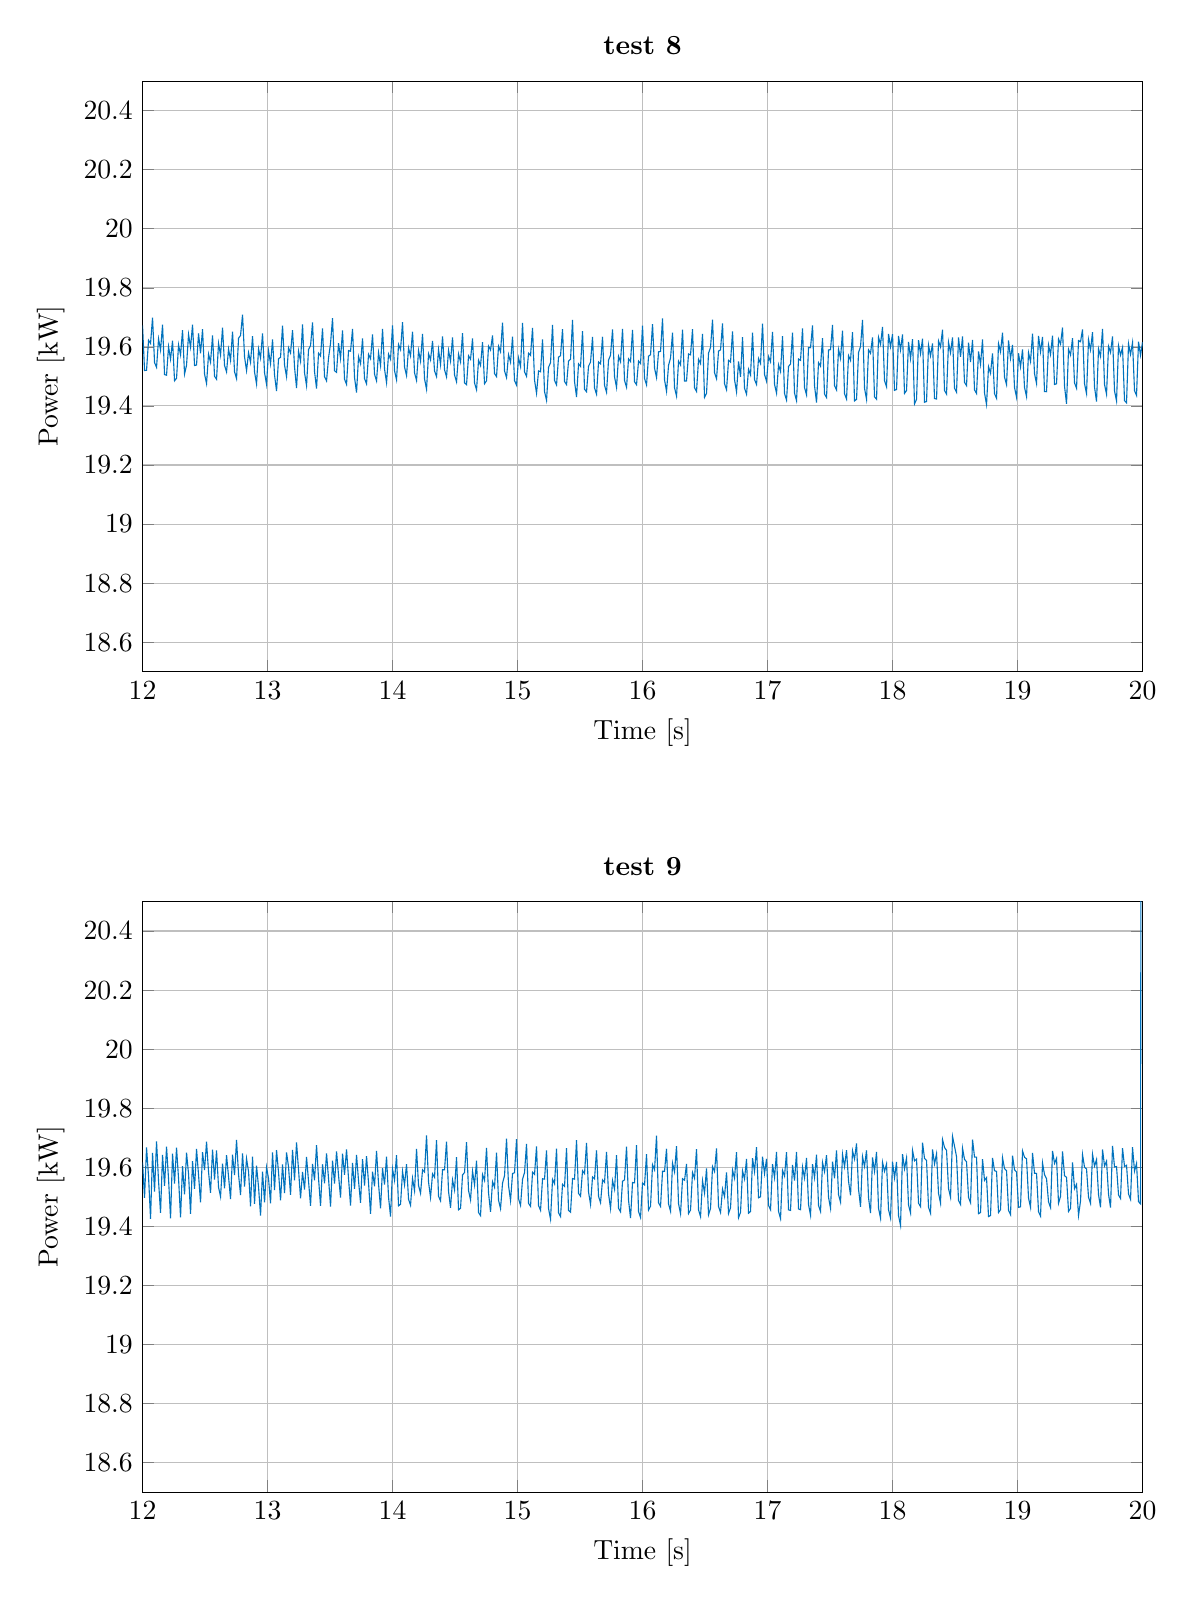
\begin{tikzpicture}

\begin{axis}[%
width=5in,
height=2.953in,
at={(1.142in,5.054in)},
scale only axis,
xmin=12,
xmax=20,
xlabel={Time [s]},
xmajorgrids,
ymin=18.5,
ymax=20.5,
ylabel={Power [kW]},
ymajorgrids,
axis background/.style={fill=white},
title style={font=\bfseries},
title={test 8}
]
\addplot [color=mycolor1,solid,forget plot]
  table[row sep=crcr]{%
12	19.672382408826\\
12.016	19.5200487760239\\
12.032	19.5205630258831\\
12.048	19.6223714241767\\
12.064	19.611413995818\\
12.08	19.6992905490012\\
12.096	19.5468508580322\\
12.112	19.5308026163444\\
12.128	19.6273050339974\\
12.144	19.5892211167947\\
12.16	19.6748762350713\\
12.176	19.5060983628349\\
12.192	19.5041347039843\\
12.208	19.6008771335158\\
12.224	19.55848684593\\
12.24	19.6209926051874\\
12.256	19.4852256355425\\
12.272	19.4937433099324\\
12.288	19.6064941867014\\
12.304	19.572975231874\\
12.32	19.656281728281\\
12.336	19.5078378620517\\
12.352	19.5380050598309\\
12.368	19.6419075107899\\
12.384	19.5989431206645\\
12.4	19.6750907225319\\
12.416	19.5368091940055\\
12.432	19.5386014376538\\
12.448	19.6459784394303\\
12.464	19.5785197039265\\
12.48	19.6598308847315\\
12.496	19.5078728401608\\
12.512	19.4758065406186\\
12.528	19.5752925472198\\
12.544	19.5480927060288\\
12.56	19.6386938257075\\
12.576	19.5004487893156\\
12.592	19.4903830374599\\
12.608	19.6116946241194\\
12.624	19.5720961587077\\
12.64	19.6654818363827\\
12.656	19.5371030450688\\
12.672	19.5151788101613\\
12.688	19.5926319230257\\
12.704	19.5544333140548\\
12.72	19.6513397496621\\
12.736	19.5156351045116\\
12.752	19.4923562362176\\
12.768	19.6294256128449\\
12.784	19.6386774675081\\
12.8	19.7092439181343\\
12.816	19.5662680609522\\
12.832	19.5195954010938\\
12.848	19.5801607648747\\
12.864	19.5475393976938\\
12.88	19.6359911887\\
12.896	19.5149523729434\\
12.912	19.4740082179797\\
12.928	19.5932285859381\\
12.944	19.5618940391613\\
12.96	19.6454075288095\\
12.976	19.5124456128073\\
12.992	19.4730629826039\\
13.008	19.5863715166506\\
13.024	19.5426738296929\\
13.04	19.624951295834\\
13.056	19.5043189979892\\
13.072	19.4500709195317\\
13.088	19.5598227612299\\
13.104	19.5646176010872\\
13.12	19.6720954862148\\
13.136	19.5384045313751\\
13.152	19.4990986045345\\
13.168	19.5964140280584\\
13.184	19.5791962158861\\
13.2	19.6566785219443\\
13.216	19.531189010192\\
13.232	19.4607916294034\\
13.248	19.5853520105484\\
13.264	19.5514870793847\\
13.28	19.6761621481474\\
13.296	19.5119529004054\\
13.312	19.468899731698\\
13.328	19.5906246208865\\
13.344	19.6041776483315\\
13.36	19.6824758310643\\
13.376	19.5160360939668\\
13.392	19.4589681964386\\
13.408	19.5786670004494\\
13.424	19.5690402292059\\
13.44	19.6627080953876\\
13.456	19.4989469086582\\
13.472	19.4848818747218\\
13.488	19.5628875216242\\
13.504	19.6120985299705\\
13.52	19.6972662226957\\
13.536	19.5192240913212\\
13.552	19.5136958099265\\
13.568	19.6124508964528\\
13.584	19.561117203315\\
13.6	19.6557562459571\\
13.616	19.4905705271867\\
13.632	19.473130551684\\
13.648	19.5874916106852\\
13.664	19.5852424057335\\
13.68	19.6605584225488\\
13.696	19.4958239449974\\
13.712	19.4452827818446\\
13.728	19.5671716341752\\
13.744	19.543107471729\\
13.76	19.6288144730102\\
13.776	19.4924967961416\\
13.792	19.4748402825493\\
13.808	19.5748644348764\\
13.824	19.559908769748\\
13.84	19.6418491984805\\
13.856	19.5072430892063\\
13.872	19.4849058242673\\
13.888	19.5805883440512\\
13.904	19.5365486176239\\
13.92	19.6609615481818\\
13.936	19.5245564961773\\
13.952	19.4787163753994\\
13.968	19.5755036527465\\
13.984	19.5579133480232\\
14	19.6727757537855\\
14.016	19.519050649704\\
14.032	19.488407468797\\
14.048	19.6080661509109\\
14.064	19.590394077618\\
14.08	19.6833247322471\\
14.096	19.531510452274\\
14.112	19.5029142513868\\
14.128	19.5961720420617\\
14.144	19.5688507497196\\
14.16	19.651118566181\\
14.176	19.5120822867722\\
14.192	19.4862725676921\\
14.208	19.5876772824666\\
14.224	19.5515612506378\\
14.24	19.6441706961489\\
14.256	19.4915293531808\\
14.272	19.4564398407227\\
14.288	19.5766848356784\\
14.304	19.5559648676418\\
14.32	19.6205070777992\\
14.336	19.5184541759484\\
14.352	19.4993838469862\\
14.368	19.5906173999031\\
14.384	19.5400467675075\\
14.4	19.6358527968791\\
14.416	19.5223937376867\\
14.432	19.498294721895\\
14.448	19.5880281096334\\
14.464	19.5515341301811\\
14.48	19.6322974209872\\
14.496	19.5046894679693\\
14.512	19.481655721186\\
14.528	19.5758905897904\\
14.544	19.548647878004\\
14.56	19.6467508790424\\
14.576	19.4782338027442\\
14.592	19.4719305702637\\
14.608	19.5699346587275\\
14.624	19.5580657212684\\
14.64	19.6283099548544\\
14.656	19.4775553078864\\
14.672	19.4547080811013\\
14.688	19.5546157270249\\
14.704	19.5369782531269\\
14.72	19.6159006107127\\
14.736	19.4751412332119\\
14.752	19.4854274002926\\
14.768	19.602611646761\\
14.784	19.5894531247944\\
14.8	19.6384550021822\\
14.816	19.509480221073\\
14.832	19.4993492245234\\
14.848	19.6022379518609\\
14.864	19.5834353961422\\
14.88	19.6818718968413\\
14.896	19.5185776136251\\
14.912	19.4960400458506\\
14.928	19.5734568081457\\
14.944	19.5478861470968\\
14.96	19.6347140029187\\
14.976	19.4857538645777\\
14.992	19.4702494015433\\
15.008	19.5622246570293\\
15.024	19.5334525962067\\
15.04	19.6808101850009\\
15.056	19.5154382291845\\
15.072	19.50020530156\\
15.088	19.5785307064857\\
15.104	19.5710321245109\\
15.12	19.6642030792386\\
15.136	19.4875606771992\\
15.152	19.4428331960114\\
15.168	19.5187019420891\\
15.184	19.5156296334776\\
15.2	19.6254244198166\\
15.216	19.4484628252316\\
15.232	19.418831202899\\
15.248	19.5307871184043\\
15.264	19.546466825207\\
15.28	19.6743005801131\\
15.296	19.4864042461646\\
15.312	19.4711810969641\\
15.328	19.5653353826864\\
15.344	19.5701213476621\\
15.36	19.6602834328498\\
15.376	19.482691232016\\
15.392	19.4721343290953\\
15.408	19.5520537124773\\
15.424	19.558140337063\\
15.44	19.691012316124\\
15.456	19.4825902106126\\
15.472	19.4303631337399\\
15.488	19.5424638817892\\
15.504	19.5339217068344\\
15.52	19.6531556330811\\
15.536	19.4565517896621\\
15.552	19.4480399440251\\
15.568	19.5346201173981\\
15.584	19.5482929810556\\
15.6	19.6335571718879\\
15.616	19.460816477236\\
15.632	19.4395309034935\\
15.648	19.5488288000156\\
15.664	19.5420275958798\\
15.68	19.6341750007665\\
15.696	19.4698866196253\\
15.712	19.4460113477953\\
15.728	19.5553866092216\\
15.744	19.5718174280794\\
15.76	19.6587916240787\\
15.776	19.4984795471067\\
15.792	19.4623312587082\\
15.808	19.5682917811016\\
15.824	19.5492414076569\\
15.84	19.6611530234308\\
15.856	19.48610035612\\
15.872	19.4632047289923\\
15.888	19.5595191327298\\
15.904	19.5502169945856\\
15.92	19.6578305164654\\
15.936	19.481989857318\\
15.952	19.4716666750204\\
15.968	19.5518841166836\\
15.984	19.5434158768066\\
16	19.6717717135769\\
16.016	19.4929434549386\\
16.032	19.4712217642828\\
16.048	19.5684731931761\\
16.064	19.5734145045483\\
16.08	19.6772983274082\\
16.096	19.5277862713285\\
16.112	19.4959865638916\\
16.128	19.5834170826514\\
16.144	19.5846574110183\\
16.16	19.6960954439298\\
16.176	19.4880914761207\\
16.192	19.4491158145389\\
16.208	19.537779445166\\
16.224	19.562544476193\\
16.24	19.6480929599977\\
16.256	19.4615280451448\\
16.272	19.4330847038225\\
16.288	19.551616315607\\
16.304	19.5387945871763\\
16.32	19.6584506997202\\
16.336	19.4840258294573\\
16.352	19.4846314998896\\
16.368	19.5760467663056\\
16.384	19.5728475487713\\
16.4	19.6597423867315\\
16.416	19.4616085661511\\
16.432	19.4488717160099\\
16.448	19.5576640804058\\
16.464	19.5432403587039\\
16.48	19.6439668029809\\
16.496	19.4291165895437\\
16.512	19.4426695467173\\
16.528	19.5789206805508\\
16.544	19.5984762781472\\
16.56	19.6919653404311\\
16.576	19.5127616492533\\
16.592	19.4921101643266\\
16.608	19.5859045521868\\
16.624	19.5899300549006\\
16.64	19.6796765403637\\
16.656	19.4753669849318\\
16.672	19.4547057665381\\
16.688	19.5544250940342\\
16.704	19.5483089919141\\
16.72	19.6522302294964\\
16.736	19.4892205495694\\
16.752	19.4474953766536\\
16.768	19.5510352075772\\
16.784	19.4982099442659\\
16.8	19.6327790822239\\
16.816	19.4596141133744\\
16.832	19.4397045720277\\
16.848	19.5241291385489\\
16.864	19.5049996838157\\
16.88	19.6485316076398\\
16.896	19.4891940278241\\
16.912	19.4726220034083\\
16.928	19.5606577689492\\
16.944	19.5435741639413\\
16.96	19.6788974047797\\
16.976	19.506326977516\\
16.992	19.4834332287929\\
17.008	19.5673599640364\\
17.024	19.5493971287919\\
17.04	19.6507284410949\\
17.056	19.4733946507159\\
17.072	19.4430376073537\\
17.088	19.5392499795136\\
17.104	19.5163900944432\\
17.12	19.6363497100307\\
17.136	19.4420605521202\\
17.152	19.4197147853296\\
17.168	19.5338197331131\\
17.184	19.541760927746\\
17.2	19.6480325547452\\
17.216	19.4432228366682\\
17.232	19.4177226546512\\
17.248	19.5589287875212\\
17.264	19.554555315252\\
17.28	19.6627451212798\\
17.296	19.4620992423539\\
17.312	19.4373461372115\\
17.328	19.5981363749286\\
17.344	19.5972953026494\\
17.36	19.6727910121237\\
17.376	19.4677826356176\\
17.392	19.4117468137087\\
17.408	19.5465135823328\\
17.424	19.5345550717387\\
17.44	19.6292170897189\\
17.456	19.4401969492418\\
17.472	19.4285586187896\\
17.488	19.5896816425881\\
17.504	19.5905788415306\\
17.52	19.6742549869105\\
17.536	19.4685176107769\\
17.552	19.4541769144032\\
17.568	19.5915525024144\\
17.584	19.5608624473552\\
17.6	19.6546208410602\\
17.616	19.4411720297858\\
17.632	19.423349074808\\
17.648	19.5702467401925\\
17.664	19.5540718378542\\
17.68	19.6494619809121\\
17.696	19.4171940162001\\
17.712	19.4221096371347\\
17.728	19.5805005430432\\
17.744	19.6013461788467\\
17.76	19.6915343386432\\
17.776	19.4597745088527\\
17.792	19.4223141675345\\
17.808	19.5896554747374\\
17.824	19.5779307063423\\
17.84	19.6322741830941\\
17.856	19.4306835874427\\
17.872	19.4228306272526\\
17.888	19.6324604094733\\
17.904	19.6082366097888\\
17.92	19.6673656305616\\
17.936	19.4857629321996\\
17.952	19.4652133186003\\
17.968	19.6440771536201\\
17.984	19.6004160673624\\
18	19.6432937570118\\
18.016	19.4528992543355\\
18.032	19.4556940678986\\
18.048	19.6367587672507\\
18.064	19.5897544162763\\
18.08	19.6419347267954\\
18.096	19.4425251115125\\
18.112	19.4520841680347\\
18.128	19.6167624521379\\
18.144	19.5607955408082\\
18.16	19.6260174071373\\
18.176	19.4069305272216\\
18.192	19.4224351943523\\
18.208	19.6227451590131\\
18.224	19.5767870866212\\
18.24	19.6277915628889\\
18.256	19.4125315760427\\
18.272	19.4150106636086\\
18.288	19.605800843366\\
18.304	19.5695193162469\\
18.32	19.6119086456511\\
18.336	19.4249499311369\\
18.352	19.4233824260443\\
18.368	19.6198645421091\\
18.384	19.5995128802492\\
18.4	19.658407757832\\
18.416	19.4523590868446\\
18.432	19.4400986860985\\
18.448	19.6157986420487\\
18.464	19.5798795282131\\
18.48	19.6321672441278\\
18.496	19.4601875230618\\
18.512	19.4467580330739\\
18.528	19.6322913530076\\
18.544	19.5661990835522\\
18.56	19.6354653965978\\
18.576	19.4797462921646\\
18.592	19.4688494144013\\
18.608	19.6141177971529\\
18.624	19.5489355512325\\
18.64	19.6232768136876\\
18.656	19.4543972042696\\
18.672	19.4421860702344\\
18.688	19.5847591493319\\
18.704	19.5406152760105\\
18.72	19.6250590197105\\
18.736	19.4435203177556\\
18.752	19.4047146739066\\
18.768	19.5329855472509\\
18.784	19.510665564001\\
18.8	19.5781078902379\\
18.816	19.4414995508044\\
18.832	19.4260571333117\\
18.848	19.6110888950271\\
18.864	19.583302321546\\
18.88	19.6480986506497\\
18.896	19.4972518216664\\
18.912	19.4721527160252\\
18.928	19.6216310741394\\
18.944	19.5609674382707\\
18.96	19.6065709558143\\
18.976	19.4621511991191\\
18.992	19.4295414290635\\
19.008	19.5782489688939\\
19.024	19.5325369750955\\
19.04	19.5912664969863\\
19.056	19.4625916935951\\
19.072	19.4316983011858\\
19.088	19.5803919968637\\
19.104	19.5502319416978\\
19.12	19.6447765670825\\
19.136	19.5093557796971\\
19.152	19.475698158319\\
19.168	19.6371300223433\\
19.184	19.5829863344606\\
19.2	19.6339661886413\\
19.216	19.4486274060438\\
19.232	19.4482343197725\\
19.248	19.6065416845847\\
19.264	19.5743906435587\\
19.28	19.6379348470856\\
19.296	19.4728763021347\\
19.312	19.4750042844557\\
19.328	19.6265055396142\\
19.344	19.6092321580651\\
19.36	19.6654465355462\\
19.376	19.4667954443762\\
19.392	19.407037561367\\
19.408	19.5922208392443\\
19.424	19.5723075269128\\
19.44	19.6296591166391\\
19.456	19.4778499322882\\
19.472	19.4599707476182\\
19.488	19.6213909530008\\
19.504	19.6174265182007\\
19.52	19.658856812839\\
19.536	19.4752036435493\\
19.552	19.4417509052717\\
19.568	19.6244049832556\\
19.584	19.5896643312036\\
19.6	19.6497059523624\\
19.616	19.4636790920773\\
19.632	19.4150949363182\\
19.648	19.5933679996792\\
19.664	19.5676900265511\\
19.68	19.6608200466611\\
19.696	19.4726240212225\\
19.712	19.4396591728644\\
19.728	19.6021381616351\\
19.744	19.5808470621479\\
19.76	19.6352592825034\\
19.776	19.4511033222695\\
19.792	19.4171266743624\\
19.808	19.6042192638725\\
19.824	19.5720541263318\\
19.84	19.5981879545034\\
19.856	19.4180826775867\\
19.872	19.4106476402165\\
19.888	19.6107039483278\\
19.904	19.57453002234\\
19.92	19.6149362637561\\
19.936	19.4516294936352\\
19.952	19.4358433080802\\
19.968	19.617484164026\\
19.984	19.5713952567739\\
20	19.6160953990141\\
20	19.6160953990141\\
};
\end{axis}

\begin{axis}[%
width=5in,
height=2.953in,
at={(1.142in,0.952in)},
scale only axis,
xmin=12,
xmax=20,
xlabel={Time [s]},
xmajorgrids,
ymin=18.5,
ymax=20.5,
ylabel={Power [kW]},
ymajorgrids,
axis background/.style={fill=white},
title style={font=\bfseries},
title={test 9}
]
\addplot [color=mycolor1,solid,forget plot]
  table[row sep=crcr]{%
12	19.6168526870486\\
12.016	19.4967812548504\\
12.032	19.6673428075204\\
12.048	19.5685362501937\\
12.064	19.4254520154133\\
12.08	19.6485523509844\\
12.096	19.5173829028733\\
12.112	19.6879746495824\\
12.128	19.5534977990005\\
12.144	19.4456216182877\\
12.16	19.6418013147459\\
12.176	19.5367875301655\\
12.192	19.669491327934\\
12.208	19.5604663877634\\
12.224	19.4269537081659\\
12.24	19.6463145897298\\
12.256	19.5451423953356\\
12.272	19.6662400268847\\
12.288	19.5623874162277\\
12.304	19.4300820143885\\
12.32	19.6040257974195\\
12.336	19.5082275082924\\
12.352	19.6496372247522\\
12.368	19.5771703933226\\
12.384	19.4422596386143\\
12.4	19.6208700689539\\
12.416	19.5266715697056\\
12.432	19.6623215694881\\
12.448	19.5735369102324\\
12.464	19.4811697141736\\
12.48	19.6513715991479\\
12.496	19.5902139870252\\
12.512	19.6865664464682\\
12.528	19.5840329076963\\
12.544	19.5135787135764\\
12.56	19.6600578146496\\
12.576	19.5582974760888\\
12.592	19.6567361757311\\
12.608	19.5323953133325\\
12.624	19.5004785282404\\
12.64	19.612606110834\\
12.656	19.5284295286328\\
12.672	19.6411109276649\\
12.688	19.5679374096194\\
12.704	19.4925671364577\\
12.72	19.6424745669571\\
12.736	19.5732350608329\\
12.752	19.6925204061834\\
12.768	19.5758872174083\\
12.784	19.5061535424533\\
12.8	19.6472224147239\\
12.816	19.5349866166657\\
12.832	19.6294245942634\\
12.848	19.5855113515485\\
12.864	19.4679800469508\\
12.88	19.6356201263834\\
12.896	19.4765615413456\\
12.912	19.6054733641549\\
12.928	19.5332006260976\\
12.944	19.4362215854725\\
12.96	19.5853004707737\\
12.976	19.4811206459633\\
12.992	19.599703800547\\
13.008	19.5616072761493\\
13.024	19.4776944049993\\
13.04	19.6500780097526\\
13.056	19.5226739234201\\
13.072	19.6583695082041\\
13.088	19.5820886572891\\
13.104	19.4883049306045\\
13.12	19.6098030219845\\
13.136	19.5124836601122\\
13.152	19.6502039118947\\
13.168	19.6011468778146\\
13.184	19.5062685894305\\
13.2	19.6592053557212\\
13.216	19.5561425086275\\
13.232	19.6840224613909\\
13.248	19.590594391827\\
13.264	19.4948860000846\\
13.28	19.583895462227\\
13.296	19.5241419090369\\
13.312	19.6347569684303\\
13.328	19.5527056740962\\
13.344	19.4697087745205\\
13.36	19.6112275060868\\
13.376	19.5561915197814\\
13.392	19.6747963368811\\
13.408	19.5621450130583\\
13.424	19.4690113262303\\
13.44	19.6101103078343\\
13.456	19.5459551793674\\
13.472	19.6472757735262\\
13.488	19.5615078278019\\
13.504	19.4671823783157\\
13.52	19.6220381345024\\
13.536	19.5448944116359\\
13.552	19.653873457305\\
13.568	19.5725831783333\\
13.584	19.4973126175747\\
13.6	19.6464874867328\\
13.616	19.5746899463403\\
13.632	19.6607596155656\\
13.648	19.5616278887626\\
13.664	19.4701419442889\\
13.68	19.614935942544\\
13.696	19.5269068547567\\
13.712	19.6422906822587\\
13.728	19.5539107931107\\
13.744	19.4795564876333\\
13.76	19.6274045740986\\
13.776	19.5379273544947\\
13.792	19.6374529782181\\
13.808	19.5467427917207\\
13.824	19.4422471286128\\
13.84	19.5848048442956\\
13.856	19.5358624661048\\
13.872	19.6557207908019\\
13.888	19.5433035607833\\
13.904	19.4607306357769\\
13.92	19.5966162318412\\
13.936	19.5417244109218\\
13.952	19.6359426062065\\
13.968	19.4986393614643\\
13.984	19.4332020328073\\
14	19.5943344000584\\
14.016	19.5561041752404\\
14.032	19.6408269088006\\
14.048	19.4695078342333\\
14.064	19.4745423825905\\
14.08	19.5862810391427\\
14.096	19.5406569065267\\
14.112	19.6106982040212\\
14.128	19.491744335905\\
14.144	19.4714829971309\\
14.16	19.5623421485599\\
14.176	19.5207181670632\\
14.192	19.6622917278204\\
14.208	19.5384620157237\\
14.224	19.5117867163422\\
14.24	19.5915931695603\\
14.256	19.583723039598\\
14.272	19.7076696676384\\
14.288	19.5501025577453\\
14.304	19.4976331293488\\
14.32	19.5780564855654\\
14.336	19.5661543795686\\
14.352	19.6915601328894\\
14.368	19.5018796158729\\
14.384	19.4862799883892\\
14.4	19.5921568281004\\
14.416	19.5913362968628\\
14.432	19.6870797012326\\
14.448	19.5185653503985\\
14.464	19.4628210049661\\
14.48	19.5572453146479\\
14.496	19.523395057706\\
14.512	19.6339731419148\\
14.528	19.4559679751342\\
14.544	19.4609862596454\\
14.56	19.5741128024666\\
14.576	19.5823650492713\\
14.592	19.6847245389773\\
14.608	19.5211429338355\\
14.624	19.4893223815971\\
14.64	19.5867145940705\\
14.656	19.5405658518703\\
14.672	19.6220576218128\\
14.688	19.4467777730798\\
14.704	19.4363269810543\\
14.72	19.575475229802\\
14.736	19.5553295353983\\
14.752	19.6653322185998\\
14.768	19.5131127568673\\
14.784	19.4490368353285\\
14.8	19.5510867627964\\
14.816	19.5323938402536\\
14.832	19.6492410628333\\
14.848	19.4882669371271\\
14.864	19.4600552862506\\
14.88	19.5466308957409\\
14.896	19.5715913278695\\
14.912	19.6967710742787\\
14.928	19.5383193486855\\
14.944	19.4870832802725\\
14.96	19.5788738270489\\
14.976	19.581615814047\\
14.992	19.6955679366377\\
15.008	19.4933225194551\\
15.024	19.470863063623\\
15.04	19.5594604986071\\
15.056	19.5822320146072\\
15.072	19.6793674784027\\
15.088	19.4780232643369\\
15.104	19.4676033752979\\
15.12	19.583326139476\\
15.136	19.576101418618\\
15.152	19.6706950747029\\
15.168	19.4704757628883\\
15.184	19.454181707975\\
15.2	19.5611138100228\\
15.216	19.5599087794067\\
15.232	19.6570724177087\\
15.248	19.4602757090314\\
15.264	19.4242277072606\\
15.28	19.5589588757459\\
15.296	19.5441660414722\\
15.312	19.6630603486119\\
15.328	19.4457851438721\\
15.344	19.4331383260088\\
15.36	19.5422664729083\\
15.376	19.5352615744007\\
15.392	19.6650702574466\\
15.408	19.4542645049774\\
15.424	19.4477918714864\\
15.44	19.5618715908735\\
15.456	19.5598959212985\\
15.472	19.6917764836458\\
15.488	19.511738607198\\
15.504	19.5018617230432\\
15.52	19.5881775735523\\
15.536	19.5784233746062\\
15.552	19.68281771675\\
15.568	19.5161661892003\\
15.584	19.4740540680588\\
15.6	19.5671132317504\\
15.616	19.5604229031689\\
15.632	19.6575527005402\\
15.648	19.5017517071369\\
15.664	19.4800520090762\\
15.68	19.5573553457206\\
15.696	19.5489731911846\\
15.712	19.6519828538061\\
15.728	19.5102432086668\\
15.744	19.4605565141136\\
15.76	19.5549716541781\\
15.776	19.5254692610156\\
15.792	19.6412594950958\\
15.808	19.4614699877475\\
15.824	19.4493315412807\\
15.84	19.5527410262357\\
15.856	19.5575200258851\\
15.872	19.6699637507695\\
15.888	19.4887114180422\\
15.904	19.427633951926\\
15.92	19.5484442670069\\
15.936	19.5473102086142\\
15.952	19.6749176703342\\
15.968	19.4502297155042\\
15.984	19.4299770396647\\
16	19.5465298432511\\
16.016	19.5399970199232\\
16.032	19.6445251803907\\
16.048	19.4552982497261\\
16.064	19.468182137872\\
16.08	19.6085851632412\\
16.096	19.5911797805367\\
16.112	19.7074135116367\\
16.128	19.4799082783376\\
16.144	19.4674209374775\\
16.16	19.5867084914399\\
16.176	19.5862981306251\\
16.192	19.6626140415005\\
16.208	19.4760053213933\\
16.224	19.4510261568988\\
16.24	19.614035825414\\
16.256	19.5846219183719\\
16.272	19.6718968621668\\
16.288	19.4764749087595\\
16.304	19.4424648034949\\
16.32	19.5611744649192\\
16.336	19.5561706120386\\
16.352	19.6111136938181\\
16.368	19.4432577724513\\
16.384	19.455320708776\\
16.4	19.5822422957405\\
16.416	19.5627765200694\\
16.432	19.6617285197741\\
16.448	19.455658103731\\
16.464	19.4329154711563\\
16.48	19.5542577235104\\
16.496	19.5127179787692\\
16.512	19.5963966129488\\
16.528	19.4391418121443\\
16.544	19.4609777833052\\
16.56	19.6021239605306\\
16.576	19.5855914423338\\
16.592	19.6636953953688\\
16.608	19.4676078940417\\
16.624	19.4467162729598\\
16.64	19.5262891767802\\
16.656	19.5007919377242\\
16.672	19.5828534570956\\
16.688	19.4434474824609\\
16.704	19.4629849914138\\
16.72	19.5901588319345\\
16.736	19.5630586902291\\
16.752	19.6510778401785\\
16.768	19.4290687589918\\
16.784	19.447750748567\\
16.8	19.5880663837792\\
16.816	19.5603810403242\\
16.832	19.6281751985716\\
16.848	19.4444543748949\\
16.864	19.4502688822884\\
16.88	19.6308849374049\\
16.896	19.5854286964478\\
16.912	19.6685135154857\\
16.928	19.4967193836731\\
16.944	19.5000704832388\\
16.96	19.6355886649016\\
16.976	19.5787634531566\\
16.992	19.6286616123841\\
17.008	19.4705679623762\\
17.024	19.4565417276069\\
17.04	19.6108494682515\\
17.056	19.5655426934453\\
17.072	19.6519117724401\\
17.088	19.4507399096144\\
17.104	19.4260884667868\\
17.12	19.5896086464906\\
17.136	19.5700262606078\\
17.152	19.6514730816879\\
17.168	19.4558050393296\\
17.184	19.4538968581841\\
17.2	19.6078775974154\\
17.216	19.5552510313973\\
17.232	19.6516545284128\\
17.248	19.4588013848938\\
17.264	19.4563606305092\\
17.28	19.6005320764993\\
17.296	19.5639380215045\\
17.312	19.631540642373\\
17.328	19.473705116412\\
17.344	19.4375783229383\\
17.36	19.6107668027669\\
17.376	19.565115804265\\
17.392	19.6427556437177\\
17.408	19.4707984144176\\
17.424	19.4503101037614\\
17.44	19.6162068853484\\
17.456	19.5853490189479\\
17.472	19.6413475637939\\
17.488	19.4982772159573\\
17.504	19.4607092025107\\
17.52	19.6193620769614\\
17.536	19.5625700876361\\
17.552	19.6571820330484\\
17.568	19.5072351263465\\
17.584	19.4819324982512\\
17.6	19.643718283408\\
17.616	19.6023274518803\\
17.632	19.6579374674793\\
17.648	19.5530127762831\\
17.664	19.5050562206317\\
17.68	19.6560637500966\\
17.696	19.6279041864596\\
17.712	19.6804833484398\\
17.728	19.5259844762617\\
17.744	19.465933310163\\
17.76	19.6359880025123\\
17.776	19.6030195341765\\
17.792	19.6574674482956\\
17.808	19.4965383308855\\
17.824	19.4447595978671\\
17.84	19.6332070885691\\
17.856	19.586322320502\\
17.872	19.6521764218289\\
17.888	19.4616714090629\\
17.904	19.4273641999615\\
17.92	19.6169639587573\\
17.936	19.5863518923032\\
17.952	19.6112404723004\\
17.968	19.4563769113134\\
17.984	19.4279731860191\\
18	19.618707314025\\
18.016	19.5644748661707\\
18.032	19.6182645479664\\
18.048	19.4362031513599\\
18.064	19.4029215347507\\
18.08	19.6447026470405\\
18.096	19.5947849819804\\
18.112	19.6315548653591\\
18.128	19.4721271233184\\
18.144	19.4449230615444\\
18.16	19.6571831146555\\
18.176	19.6218513857228\\
18.192	19.6275436717692\\
18.208	19.4783737915623\\
18.224	19.4665503528464\\
18.24	19.6835204277381\\
18.256	19.6297227569184\\
18.272	19.623244182143\\
18.288	19.4647024697246\\
18.304	19.4446134070446\\
18.32	19.6604259453459\\
18.336	19.6115780864593\\
18.352	19.6456932539215\\
18.368	19.5116730480609\\
18.384	19.4783856984523\\
18.4	19.6939182345005\\
18.416	19.6666737704681\\
18.432	19.6574198619125\\
18.448	19.5278978633189\\
18.464	19.4983710209929\\
18.48	19.7046012485589\\
18.496	19.6713062256131\\
18.512	19.6359494137036\\
18.528	19.4873674184284\\
18.544	19.4740929973276\\
18.56	19.6645105771656\\
18.576	19.6266827107153\\
18.592	19.6185980042707\\
18.608	19.497921183106\\
18.624	19.480145216093\\
18.64	19.6938767608429\\
18.656	19.6346168282624\\
18.672	19.6343212316351\\
18.688	19.4428968187173\\
18.704	19.4466688030029\\
18.72	19.6276028229192\\
18.736	19.555434609779\\
18.752	19.5649262971669\\
18.768	19.433044391688\\
18.784	19.4366029203837\\
18.8	19.6318510580414\\
18.816	19.5882382639034\\
18.832	19.5861827487702\\
18.848	19.4467467103361\\
18.864	19.4563138494828\\
18.88	19.6325297168222\\
18.896	19.595299171492\\
18.912	19.5881285924628\\
18.928	19.4542772946722\\
18.944	19.4396965435364\\
18.96	19.6394384411796\\
18.976	19.5915842100159\\
18.992	19.5841170417464\\
19.008	19.4642455963783\\
19.024	19.4662391701854\\
19.04	19.6552807452216\\
19.056	19.6337064130135\\
19.072	19.6287989947002\\
19.088	19.4959291504137\\
19.104	19.4641513396701\\
19.12	19.6483437364613\\
19.136	19.5798541990859\\
19.152	19.5794075868736\\
19.168	19.4495818086531\\
19.184	19.434650545676\\
19.2	19.6145409469759\\
19.216	19.5747719137971\\
19.232	19.5615636682158\\
19.248	19.4827934419023\\
19.264	19.4636564164556\\
19.28	19.6556421050154\\
19.296	19.6131453666208\\
19.312	19.6302888016731\\
19.328	19.4781425657558\\
19.344	19.5014286419054\\
19.36	19.6534248013804\\
19.376	19.5713029584536\\
19.392	19.5659047512953\\
19.408	19.4503519483947\\
19.424	19.4608966799986\\
19.44	19.6162864084448\\
19.456	19.5276366808905\\
19.472	19.542139947425\\
19.488	19.4368358226213\\
19.504	19.4857827690819\\
19.52	19.642889281146\\
19.536	19.6003420323905\\
19.552	19.5943884190088\\
19.568	19.4987557956077\\
19.584	19.477653892213\\
19.6	19.6438410411232\\
19.616	19.6039955823916\\
19.632	19.6261767762666\\
19.648	19.5068953881005\\
19.664	19.4647661402278\\
19.68	19.6601027089037\\
19.696	19.6046161868338\\
19.712	19.6208671789626\\
19.728	19.5085923999741\\
19.744	19.4636766789229\\
19.76	19.6727399484437\\
19.776	19.6009148083797\\
19.792	19.6024860980546\\
19.808	19.5062457290135\\
19.824	19.4942537539881\\
19.84	19.6646075390331\\
19.856	19.6025056291149\\
19.872	19.6068841300065\\
19.888	19.5094857840514\\
19.904	19.4915276052623\\
19.92	19.6682503007674\\
19.936	19.5872707260384\\
19.952	19.6130696119581\\
19.968	19.4836393308965\\
19.984	19.4761857302346\\
19.9873728101662	20.7\\
};
\end{axis}
\end{tikzpicture}%
% \caption{Steady state power output of the genset at 20 kW load.}
% \label{fig:test8-9steadypower20kw}
% \end{figure}

% \begin{figure}[H]
% \centering
% % This file was created by matlab2tikz.
%
%The latest updates can be retrieved from
%  http://www.mathworks.com/matlabcentral/fileexchange/22022-matlab2tikz-matlab2tikz
%where you can also make suggestions and rate matlab2tikz.
%
\definecolor{mycolor1}{rgb}{0.00000,0.44700,0.74100}%
%
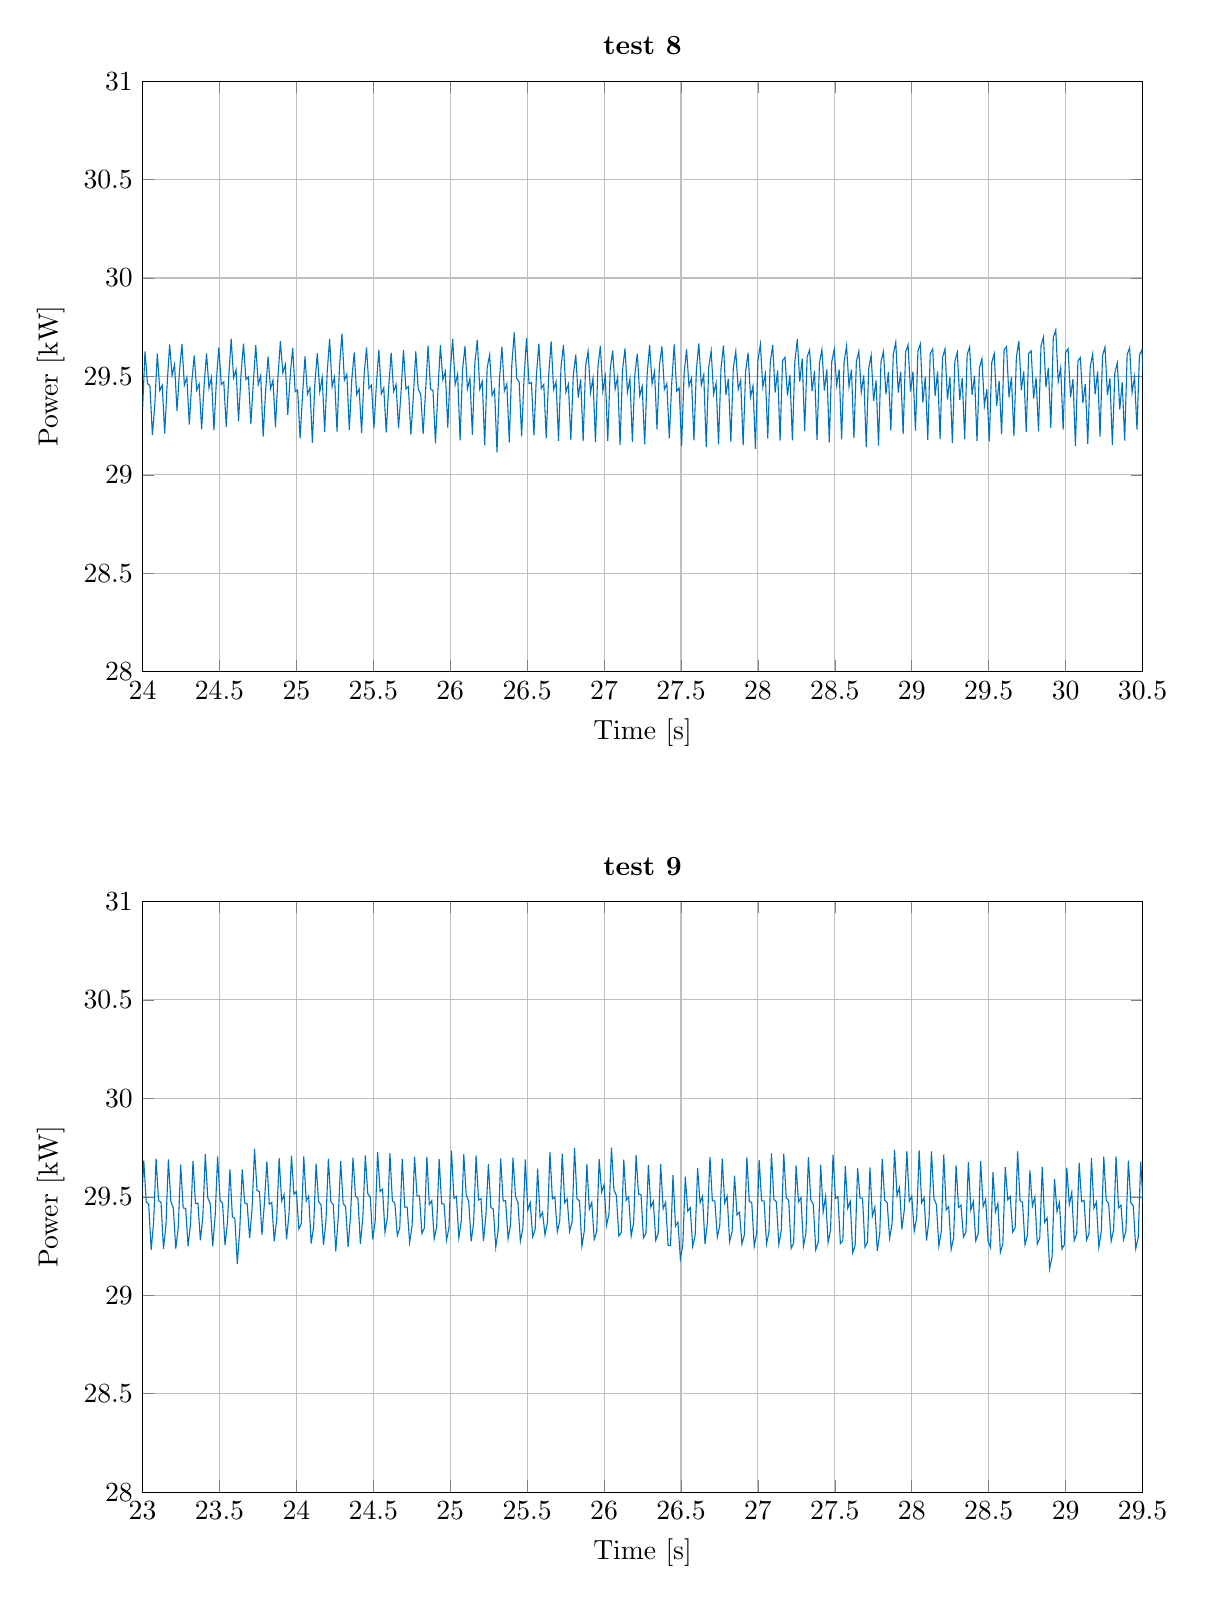
\begin{tikzpicture}

\begin{axis}[%
width=5in,
height=2.953in,
at={(1.142in,5.054in)},
scale only axis,
xmin=24,
xmax=30.5,
xlabel={Time [s]},
xmajorgrids,
ymin=28,
ymax=31,
ylabel={Power [kW]},
ymajorgrids,
axis background/.style={fill=white},
title style={font=\bfseries},
title={test 8}
]
\addplot [color=mycolor1,solid,forget plot]
  table[row sep=crcr]{%
24	29.328170239195\\
24.016	29.627315872157\\
24.032	29.4640791462457\\
24.048	29.4519030432502\\
24.064	29.2013285919211\\
24.08	29.3597309312137\\
24.096	29.6173736433362\\
24.112	29.4283947035307\\
24.128	29.4549720998017\\
24.144	29.2098043042457\\
24.16	29.4610402018116\\
24.176	29.6626361915609\\
24.192	29.5046951199298\\
24.208	29.5605709195911\\
24.224	29.3253326991344\\
24.24	29.5257523517466\\
24.256	29.6634959849433\\
24.272	29.4559710076124\\
24.288	29.494564036522\\
24.304	29.2548280353941\\
24.32	29.4725092890054\\
24.336	29.606714253325\\
24.352	29.4302103710441\\
24.368	29.4618787105569\\
24.384	29.2312031997243\\
24.4	29.4537569858665\\
24.416	29.6162033258584\\
24.432	29.4405651754057\\
24.448	29.4944422738692\\
24.464	29.2268600760824\\
24.48	29.4790852412078\\
24.496	29.6472091335788\\
24.512	29.4587329742119\\
24.528	29.4726123541534\\
24.544	29.2441559635418\\
24.56	29.4897672421324\\
24.576	29.6911878997582\\
24.592	29.4935302483806\\
24.608	29.5332937429689\\
24.624	29.2722242436429\\
24.64	29.5067204631821\\
24.656	29.666511031211\\
24.672	29.4842861894421\\
24.688	29.4975155179796\\
24.704	29.2584262901394\\
24.72	29.4676441596279\\
24.736	29.6587750065477\\
24.752	29.4584550046005\\
24.768	29.5036152189178\\
24.784	29.1947652175148\\
24.8	29.428026963411\\
24.816	29.6013256429514\\
24.832	29.4378624674673\\
24.848	29.4801727953723\\
24.864	29.2416533362681\\
24.88	29.4949158551085\\
24.896	29.6789031651815\\
24.912	29.5178929519904\\
24.928	29.5604351846232\\
24.944	29.3049745763599\\
24.96	29.5042702596805\\
24.976	29.6446709765497\\
24.992	29.4223884693646\\
25.008	29.4308900176188\\
25.024	29.1860016621515\\
25.04	29.4043502792146\\
25.056	29.6018221733937\\
25.072	29.4095182670484\\
25.088	29.4420319579254\\
25.104	29.1619034743373\\
25.12	29.4625624513762\\
25.136	29.6184955178272\\
25.152	29.4228758258205\\
25.168	29.4935733607827\\
25.184	29.2179489328206\\
25.2	29.5186517832885\\
25.216	29.6909937310951\\
25.232	29.4473942682431\\
25.248	29.4970538544955\\
25.264	29.2197965720642\\
25.28	29.5459606533496\\
25.296	29.7167185506597\\
25.312	29.4809526450029\\
25.328	29.5120695809606\\
25.344	29.2279516220808\\
25.36	29.4835329359249\\
25.376	29.6220914503873\\
25.392	29.4083491577685\\
25.408	29.4364700160061\\
25.424	29.2123311446766\\
25.44	29.5053017363494\\
25.456	29.6473902083525\\
25.472	29.438684909583\\
25.488	29.4557866316733\\
25.504	29.2365893752164\\
25.52	29.4586283698051\\
25.536	29.6341707106287\\
25.552	29.4112903359052\\
25.568	29.4413071320589\\
25.584	29.2160853816861\\
25.6	29.4437381899055\\
25.616	29.6202240311145\\
25.632	29.4233813010915\\
25.648	29.4589386312163\\
25.664	29.2358769963237\\
25.68	29.4170349965684\\
25.696	29.6351437727817\\
25.712	29.4363726490517\\
25.728	29.4487122658258\\
25.744	29.2045315018038\\
25.76	29.3925937362083\\
25.776	29.6269527150606\\
25.792	29.4351994154038\\
25.808	29.4099515408106\\
25.824	29.2082340811629\\
25.84	29.429257745232\\
25.856	29.6562041485452\\
25.872	29.4375501268908\\
25.888	29.4265211599121\\
25.904	29.160277766916\\
25.92	29.4268760886205\\
25.936	29.6580826113337\\
25.952	29.4833835071099\\
25.968	29.5243262439104\\
25.984	29.2402322122282\\
26	29.5267034595137\\
26.016	29.6902988641544\\
26.032	29.4586583391152\\
26.048	29.5116105950572\\
26.064	29.1754681992333\\
26.08	29.5352103304659\\
26.096	29.6531798938637\\
26.112	29.4368990340049\\
26.128	29.4884216026876\\
26.144	29.2029201552661\\
26.16	29.5677130276873\\
26.176	29.685208646606\\
26.192	29.4346585160104\\
26.208	29.4742646874202\\
26.224	29.1499230311345\\
26.24	29.541989420329\\
26.256	29.6094604266519\\
26.272	29.4036753631393\\
26.288	29.4338521715679\\
26.304	29.114232676981\\
26.32	29.4858773593082\\
26.336	29.6507320424194\\
26.352	29.4261091535841\\
26.368	29.4620532987719\\
26.384	29.1656103425163\\
26.4	29.5554702742668\\
26.416	29.7231164821786\\
26.432	29.4910241267143\\
26.448	29.4718740916746\\
26.464	29.1954965856704\\
26.48	29.4943150231371\\
26.496	29.6947492847567\\
26.512	29.4639453750199\\
26.528	29.4683335643679\\
26.544	29.2006511687785\\
26.56	29.501978541615\\
26.576	29.666555594122\\
26.592	29.4390641824899\\
26.608	29.4592079395061\\
26.624	29.1860826298154\\
26.64	29.5072285564055\\
26.656	29.6774865752895\\
26.672	29.4332245457345\\
26.688	29.4724307111036\\
26.704	29.1729064212038\\
26.72	29.5464742553925\\
26.736	29.659937177996\\
26.752	29.4204215902019\\
26.768	29.460093585823\\
26.784	29.1773134984552\\
26.8	29.5049297446532\\
26.816	29.610692973042\\
26.832	29.3923987250113\\
26.848	29.4851589977078\\
26.864	29.1718858659192\\
26.88	29.5538446605208\\
26.896	29.6277372621368\\
26.912	29.4175289291243\\
26.928	29.490939478243\\
26.944	29.1652869612265\\
26.96	29.5484484276675\\
26.976	29.6550801948032\\
26.992	29.4262082431191\\
27.008	29.5016432897874\\
27.024	29.1728005739131\\
27.04	29.5380746661095\\
27.056	29.6307929126049\\
27.072	29.4359804099415\\
27.088	29.4962065044839\\
27.104	29.1512771792832\\
27.12	29.5326870878015\\
27.136	29.6422874324036\\
27.152	29.4206282087608\\
27.168	29.4877782795226\\
27.184	29.1675599217065\\
27.2	29.5086011770382\\
27.216	29.6159681941651\\
27.232	29.4018934131922\\
27.248	29.4489547487222\\
27.264	29.1544723447464\\
27.28	29.5103863809196\\
27.296	29.6605678263485\\
27.312	29.4629656585395\\
27.328	29.5257000781859\\
27.344	29.2314875848801\\
27.36	29.5560340839748\\
27.376	29.6526658647445\\
27.392	29.4336381191526\\
27.408	29.4632638919827\\
27.424	29.1851468962855\\
27.44	29.4695797785302\\
27.456	29.6626386886528\\
27.472	29.4251384955891\\
27.488	29.441430435014\\
27.504	29.1462085678045\\
27.52	29.510257578279\\
27.536	29.638501896566\\
27.552	29.4514858133067\\
27.568	29.4911805750337\\
27.584	29.1750037255912\\
27.6	29.5331269753182\\
27.616	29.6674021497853\\
27.632	29.4558068606158\\
27.648	29.5077874356762\\
27.664	29.1403777159135\\
27.68	29.5447919504651\\
27.696	29.6299783980113\\
27.712	29.4106847598135\\
27.728	29.4660278761382\\
27.744	29.1553723048933\\
27.76	29.5391620013294\\
27.776	29.6579073184635\\
27.792	29.4056714357567\\
27.808	29.4885487770938\\
27.824	29.1681262487785\\
27.84	29.5428268515123\\
27.856	29.6273816813407\\
27.872	29.4343357563502\\
27.888	29.4798281793723\\
27.904	29.1494327906194\\
27.92	29.5233483940872\\
27.936	29.6200021701822\\
27.952	29.3954137294178\\
27.968	29.4516126649397\\
27.984	29.1322421124656\\
28	29.5787415639712\\
28.016	29.6635811602907\\
28.032	29.4466461541976\\
28.048	29.5121809899651\\
28.064	29.1856830459182\\
28.08	29.56859297968\\
28.096	29.6593346525922\\
28.112	29.4182749825913\\
28.128	29.530801304364\\
28.144	29.1742644988947\\
28.16	29.5795781212191\\
28.176	29.5965205821964\\
28.192	29.4021835286181\\
28.208	29.5067629517815\\
28.224	29.1745547779651\\
28.24	29.5726748445078\\
28.256	29.6886152617581\\
28.272	29.4741695756394\\
28.288	29.5899680912343\\
28.304	29.2236976725414\\
28.32	29.5989377258104\\
28.336	29.634285918878\\
28.352	29.4250637225018\\
28.368	29.5270020382906\\
28.384	29.1758331895904\\
28.4	29.5685085648503\\
28.416	29.6363574758639\\
28.432	29.4280422577218\\
28.448	29.5360692773079\\
28.464	29.1650519159091\\
28.48	29.5751359839687\\
28.496	29.6373843791839\\
28.512	29.4546626335827\\
28.528	29.5353767665109\\
28.544	29.1808617272183\\
28.56	29.5720013775435\\
28.576	29.6551998231612\\
28.592	29.4489700338986\\
28.608	29.5348096202514\\
28.624	29.1861335304816\\
28.64	29.5757274615416\\
28.656	29.6271282161883\\
28.672	29.4196310512029\\
28.688	29.5046157465958\\
28.704	29.1406974449896\\
28.72	29.5383820955435\\
28.736	29.6078854306412\\
28.752	29.3752921307144\\
28.768	29.4797298631557\\
28.784	29.1487582285931\\
28.8	29.5738205827566\\
28.816	29.6263441975822\\
28.832	29.4093806014315\\
28.848	29.5213364731303\\
28.864	29.2250991508848\\
28.88	29.6110710404561\\
28.896	29.67368638552\\
28.912	29.4181475220467\\
28.928	29.52236933214\\
28.944	29.2072593671472\\
28.96	29.6234483105293\\
28.976	29.6599201972387\\
28.992	29.4224968723579\\
29.008	29.5238668595099\\
29.024	29.2248670639798\\
29.04	29.6273359189405\\
29.056	29.6646592499103\\
29.072	29.367042651155\\
29.088	29.497701321106\\
29.104	29.1772677242347\\
29.12	29.6150193425409\\
29.136	29.6392977986934\\
29.152	29.4010278959116\\
29.168	29.5255165997802\\
29.184	29.1812909054138\\
29.2	29.5964022590995\\
29.216	29.6397408581071\\
29.232	29.3826688497321\\
29.248	29.4957987980682\\
29.264	29.1607081128388\\
29.28	29.5759147709069\\
29.296	29.6219617334158\\
29.312	29.3812339771804\\
29.328	29.4912344647844\\
29.344	29.1813261634444\\
29.36	29.608986336113\\
29.376	29.650151740476\\
29.392	29.4063558450966\\
29.408	29.5032208028625\\
29.424	29.1710714076388\\
29.44	29.5443126806331\\
29.456	29.5897003285013\\
29.472	29.352027675048\\
29.488	29.4346008382836\\
29.504	29.1695776683345\\
29.52	29.570080359218\\
29.536	29.6160273605029\\
29.552	29.3511016698829\\
29.568	29.4768679058169\\
29.584	29.2057276713289\\
29.6	29.6336517398219\\
29.616	29.6511518581276\\
29.632	29.3933577803969\\
29.648	29.4968915711386\\
29.664	29.1973464150105\\
29.68	29.5973744862271\\
29.696	29.6802413357355\\
29.712	29.4300285322573\\
29.728	29.525026069002\\
29.744	29.217317266989\\
29.76	29.616609470073\\
29.776	29.6304567848748\\
29.792	29.3877852903727\\
29.808	29.4942637380197\\
29.824	29.2210208896501\\
29.84	29.6552654954614\\
29.856	29.6996615460481\\
29.872	29.4452434016766\\
29.888	29.543907640496\\
29.904	29.2381206572316\\
29.92	29.6974830384827\\
29.936	29.736010800202\\
29.952	29.4736271991649\\
29.968	29.5441239162902\\
29.984	29.2300041264682\\
30	29.6227479524045\\
30.016	29.6404610002091\\
30.032	29.3945939297975\\
30.048	29.4857323312292\\
30.064	29.1459706963918\\
30.08	29.5775941377823\\
30.096	29.5957857404505\\
30.112	29.3660784201831\\
30.128	29.4617837779809\\
30.144	29.1577265954925\\
30.16	29.5483210927577\\
30.176	29.614059443821\\
30.192	29.4086363756863\\
30.208	29.5249531421738\\
30.224	29.1937992208752\\
30.24	29.60629536893\\
30.256	29.6484308126304\\
30.272	29.4057391415188\\
30.288	29.4902809779546\\
30.304	29.150894849733\\
30.32	29.5180703937708\\
30.336	29.5685875953455\\
30.352	29.3332455879012\\
30.368	29.4700996575894\\
30.384	29.1738840573934\\
30.4	29.6095268031999\\
30.416	29.6453647632967\\
30.432	29.4183151749128\\
30.448	29.4972206973919\\
30.464	29.229194427805\\
30.48	29.6081208841464\\
30.496	29.6348465677989\\
30.512	29.400534547486\\
};
\end{axis}

\begin{axis}[%
width=5in,
height=2.953in,
at={(1.142in,0.952in)},
scale only axis,
xmin=23,
xmax=29.5,
xlabel={Time [s]},
xmajorgrids,
ymin=28,
ymax=31,
ylabel={Power [kW]},
ymajorgrids,
axis background/.style={fill=white},
title style={font=\bfseries},
title={test 9}
]
\addplot [color=mycolor1,solid,forget plot]
  table[row sep=crcr]{%
22.992	29.4380989019936\\
23.008	29.683839540161\\
23.024	29.4728146367054\\
23.04	29.462287865334\\
23.056	29.2304724923611\\
23.072	29.3711565154849\\
23.088	29.6938014530245\\
23.104	29.4800720135832\\
23.12	29.4726002584185\\
23.136	29.2361745002338\\
23.152	29.3531401971822\\
23.168	29.6897740622715\\
23.184	29.4753941406419\\
23.2	29.4439339903873\\
23.216	29.2370953562167\\
23.232	29.3423841997204\\
23.248	29.6630213312501\\
23.264	29.4432543219668\\
23.28	29.4413894804318\\
23.296	29.2486478921835\\
23.312	29.3642541399535\\
23.328	29.6829828138914\\
23.344	29.4659887989296\\
23.36	29.4680153497842\\
23.376	29.2788474995186\\
23.392	29.3995830909535\\
23.408	29.7167041770418\\
23.424	29.4949733480101\\
23.44	29.4652940309299\\
23.456	29.2478855338465\\
23.472	29.4032477347252\\
23.488	29.7046608870887\\
23.504	29.483497948612\\
23.52	29.4666388218843\\
23.536	29.2542249696333\\
23.552	29.3673306577874\\
23.568	29.639251134813\\
23.584	29.3987430913234\\
23.6	29.3896184063222\\
23.616	29.1599150368842\\
23.632	29.3343175729058\\
23.648	29.638729631219\\
23.664	29.4691067608605\\
23.68	29.4644591627248\\
23.696	29.2898805307263\\
23.712	29.4409976437192\\
23.728	29.7427164268661\\
23.744	29.5332406055399\\
23.76	29.5255020921087\\
23.776	29.3077555315407\\
23.792	29.4653492275284\\
23.808	29.6796131531515\\
23.824	29.4626243231626\\
23.84	29.4712070545249\\
23.856	29.2739193524415\\
23.872	29.3844103373025\\
23.888	29.6964697087759\\
23.904	29.4792120960275\\
23.92	29.5112563189616\\
23.936	29.2842324626567\\
23.952	29.4111568926124\\
23.968	29.7091468047603\\
23.984	29.5133045141611\\
24	29.5270279380554\\
24.016	29.3366428320268\\
24.032	29.3642262698354\\
24.048	29.7046708477826\\
24.064	29.4787998878566\\
24.08	29.5034198813494\\
24.096	29.2624553173498\\
24.112	29.3475348298968\\
24.128	29.668148874955\\
24.144	29.4765939194851\\
24.16	29.4588694238307\\
24.176	29.2555745865971\\
24.192	29.3736165472091\\
24.208	29.6935086936868\\
24.224	29.4757014210685\\
24.24	29.4594037260083\\
24.256	29.2235014190376\\
24.272	29.3942739499664\\
24.288	29.6815773537889\\
24.304	29.4648975735428\\
24.32	29.4501148730881\\
24.336	29.2450721198562\\
24.352	29.404423968494\\
24.368	29.6990826470816\\
24.384	29.5034954403484\\
24.4	29.4928210063589\\
24.416	29.26091784725\\
24.432	29.3952081528613\\
24.448	29.7104738986048\\
24.464	29.5157480353417\\
24.48	29.4993426394281\\
24.496	29.2834878824247\\
24.512	29.3746508837599\\
24.528	29.726403587194\\
24.544	29.526994998403\\
24.56	29.5387795169389\\
24.576	29.3194736193888\\
24.592	29.3972082220104\\
24.608	29.72165033353\\
24.624	29.4798597087779\\
24.64	29.4678519578665\\
24.656	29.3029962988635\\
24.672	29.3418541200428\\
24.688	29.6919611124776\\
24.704	29.4483406487216\\
24.72	29.4478407392504\\
24.736	29.2679582848727\\
24.752	29.3535306813778\\
24.768	29.7044342671964\\
24.784	29.5049444354855\\
24.8	29.5038951990258\\
24.816	29.3139944460786\\
24.832	29.3416935399762\\
24.848	29.7038350730206\\
24.864	29.4606531847976\\
24.88	29.4807673307166\\
24.896	29.2870472195989\\
24.912	29.3489778762737\\
24.928	29.6924115591442\\
24.944	29.4647010413433\\
24.96	29.4640163205284\\
24.976	29.2800174259406\\
24.992	29.3419734526262\\
25.008	29.7350420603985\\
25.024	29.4930426090088\\
25.04	29.5020482888349\\
25.056	29.2913178166025\\
25.072	29.3774979205261\\
25.088	29.7160514321193\\
25.104	29.5086788667244\\
25.12	29.4773725947061\\
25.136	29.2737611463114\\
25.152	29.3685637849858\\
25.168	29.7099971388203\\
25.184	29.4836118728363\\
25.2	29.4900685101835\\
25.216	29.2745888834435\\
25.232	29.4065401055614\\
25.248	29.665729399064\\
25.264	29.4460260335376\\
25.28	29.4374133459474\\
25.296	29.2437500597881\\
25.312	29.333165338226\\
25.328	29.6934708749714\\
25.344	29.4783170148525\\
25.36	29.480572829145\\
25.376	29.2865136870188\\
25.392	29.3589638678085\\
25.408	29.6992115945848\\
25.424	29.5023253810741\\
25.44	29.4707496457464\\
25.456	29.2738529631555\\
25.472	29.3406567710234\\
25.488	29.690428972212\\
25.504	29.4321768378736\\
25.52	29.4697483569061\\
25.536	29.2973363802006\\
25.552	29.3339740622183\\
25.568	29.6434411543232\\
25.584	29.3954953822025\\
25.6	29.4211360527159\\
25.616	29.306628008104\\
25.632	29.3709489342178\\
25.648	29.7267036542297\\
25.664	29.4896900410667\\
25.68	29.5004556270153\\
25.696	29.3222380891049\\
25.712	29.3785918857067\\
25.728	29.7185353625932\\
25.744	29.4698489596164\\
25.76	29.4892666150257\\
25.776	29.3243481608473\\
25.792	29.3736156573387\\
25.808	29.7487337899198\\
25.824	29.4907060377542\\
25.84	29.4791622744562\\
25.856	29.2484912604409\\
25.872	29.3296925252377\\
25.888	29.6662837258739\\
25.904	29.4364919491782\\
25.92	29.471655392183\\
25.936	29.2837231506285\\
25.952	29.3231891802155\\
25.968	29.6919287679378\\
25.984	29.5235984990997\\
26	29.5611559069335\\
26.016	29.3546064904403\\
26.032	29.4129011491734\\
26.048	29.7498699055829\\
26.064	29.5347347048585\\
26.08	29.5065828737473\\
26.096	29.3009378511836\\
26.112	29.3198243167914\\
26.128	29.6883246693285\\
26.144	29.4823293682617\\
26.16	29.5000564334355\\
26.176	29.3000825397988\\
26.192	29.3676819594585\\
26.208	29.7123091894649\\
26.224	29.5129372541162\\
26.24	29.5123897415398\\
26.256	29.2911315374186\\
26.272	29.3143400230385\\
26.288	29.6623782807334\\
26.304	29.4468425627293\\
26.32	29.4775344393372\\
26.336	29.2785407827931\\
26.352	29.315403220209\\
26.368	29.6653534526469\\
26.384	29.4390378405648\\
26.4	29.4720632623062\\
26.416	29.2537038528757\\
26.432	29.2524924284121\\
26.448	29.6116925398991\\
26.464	29.3508604572854\\
26.48	29.3718648159102\\
26.496	29.1844232959222\\
26.512	29.256697422219\\
26.528	29.6027015486217\\
26.544	29.4269625938332\\
26.56	29.4450240156056\\
26.576	29.2486450959367\\
26.592	29.3039592893412\\
26.608	29.6470985352547\\
26.624	29.4695646715608\\
26.64	29.5027757944906\\
26.656	29.2595996275422\\
26.672	29.372308817957\\
26.688	29.7014599604091\\
26.704	29.479302690344\\
26.72	29.4794305483902\\
26.736	29.2950830137307\\
26.752	29.3549016347447\\
26.768	29.6937043974282\\
26.784	29.4688784895845\\
26.8	29.5021652436304\\
26.816	29.2726393507899\\
26.832	29.3214441918375\\
26.848	29.6075072263466\\
26.864	29.4083890737451\\
26.88	29.4218140493601\\
26.896	29.2606435459035\\
26.912	29.3064502245463\\
26.928	29.6996633047018\\
26.944	29.4762399763374\\
26.96	29.4702681392536\\
26.976	29.2485462268959\\
26.992	29.3164396517402\\
27.008	29.6872561583251\\
27.024	29.4795308697454\\
27.04	29.4794758149344\\
27.056	29.2609069685092\\
27.072	29.3228197263404\\
27.088	29.7200700927059\\
27.104	29.4866470388034\\
27.12	29.4747890556503\\
27.136	29.2581223150612\\
27.152	29.3313700012505\\
27.168	29.7188426055759\\
27.184	29.4965900530781\\
27.2	29.4822746016449\\
27.216	29.2376655677479\\
27.232	29.2630611330926\\
27.248	29.6589495118462\\
27.264	29.4739165003431\\
27.28	29.4950266868671\\
27.296	29.2500486577393\\
27.312	29.3143757769006\\
27.328	29.7012433018731\\
27.344	29.4826015110819\\
27.36	29.4615470229857\\
27.376	29.2302351406872\\
27.392	29.2687557521814\\
27.408	29.6615273219666\\
27.424	29.4227983137271\\
27.44	29.5020312874074\\
27.456	29.2678935979022\\
27.472	29.3292333330589\\
27.488	29.7137000268881\\
27.504	29.4924473295791\\
27.52	29.5011769925893\\
27.536	29.2625486717098\\
27.552	29.278089035936\\
27.568	29.6552177466111\\
27.584	29.4423034254276\\
27.6	29.4768644034302\\
27.616	29.215977622748\\
27.632	29.2532104600605\\
27.648	29.6462024987666\\
27.664	29.4938040986937\\
27.68	29.4928554216519\\
27.696	29.243789350876\\
27.712	29.2689122386764\\
27.728	29.649150717921\\
27.744	29.4022188856756\\
27.76	29.447372835\\
27.776	29.2256760217143\\
27.792	29.315108843359\\
27.808	29.6931233592815\\
27.824	29.482680246095\\
27.84	29.4713905755453\\
27.856	29.2902687483946\\
27.872	29.3628312300401\\
27.888	29.7398003678775\\
27.904	29.5059391570091\\
27.92	29.5473045159212\\
27.936	29.3350925531796\\
27.952	29.4375623065794\\
27.968	29.7320280019306\\
27.984	29.4772174057667\\
28	29.5032956317229\\
28.016	29.3256613369006\\
28.032	29.3934512197422\\
28.048	29.7362359898677\\
28.064	29.469944904922\\
28.08	29.4948209357664\\
28.096	29.2773660060098\\
28.112	29.382578458199\\
28.128	29.7308737463047\\
28.144	29.4903900581413\\
28.16	29.4616069945815\\
28.176	29.2493312275592\\
28.192	29.3241279385571\\
28.208	29.7147844458857\\
28.224	29.4328304743345\\
28.24	29.4510362212569\\
28.256	29.2327844362996\\
28.272	29.29104395654\\
28.288	29.660107883131\\
28.304	29.4460194355248\\
28.32	29.4578572242717\\
28.336	29.2950694756864\\
28.352	29.3190362652729\\
28.368	29.6764731315185\\
28.384	29.4328725419383\\
28.4	29.4769777906543\\
28.416	29.2765497108708\\
28.432	29.3131900442431\\
28.448	29.6809179598308\\
28.464	29.4512514350824\\
28.48	29.4870236302677\\
28.496	29.2762878987443\\
28.512	29.2421790488535\\
28.528	29.6246751486744\\
28.544	29.4238978916964\\
28.56	29.4654311902786\\
28.576	29.2179704798438\\
28.592	29.2607291403564\\
28.608	29.6510719946661\\
28.624	29.4844514025325\\
28.64	29.5024834886834\\
28.656	29.3214495557619\\
28.672	29.3431574072529\\
28.688	29.7312976397687\\
28.704	29.4801492747503\\
28.72	29.4719488542378\\
28.736	29.2573420126774\\
28.752	29.3046917789008\\
28.768	29.6340003749349\\
28.784	29.4527877564598\\
28.8	29.4984499711449\\
28.816	29.2590620479429\\
28.832	29.2909980235583\\
28.848	29.6518428310414\\
28.864	29.3713660550327\\
28.88	29.3932818526057\\
28.896	29.1348815783315\\
28.912	29.1947162157334\\
28.928	29.591154332406\\
28.944	29.4253489228846\\
28.96	29.4715627880898\\
28.976	29.2343762211789\\
28.992	29.257367624145\\
29.008	29.6477908519129\\
29.024	29.4602836018971\\
29.04	29.5227425394681\\
29.056	29.2765175564079\\
29.072	29.3132887085799\\
29.088	29.6729448038455\\
29.104	29.4762102047806\\
29.12	29.4817128487599\\
29.136	29.2798201277527\\
29.152	29.3125255668568\\
29.168	29.6962509405528\\
29.184	29.442405765922\\
29.2	29.4730406894579\\
29.216	29.2435662909061\\
29.232	29.3244889919582\\
29.248	29.7035094980585\\
29.264	29.4828413228856\\
29.28	29.4648363450623\\
29.296	29.2745044774062\\
29.312	29.3325112510697\\
29.328	29.705035056432\\
29.344	29.4438810384003\\
29.36	29.4574207535976\\
29.376	29.2823656033441\\
29.392	29.325425347315\\
29.408	29.6838007921575\\
29.424	29.4688224647317\\
29.44	29.453710148573\\
29.456	29.2366244623443\\
29.472	29.293821178617\\
29.488	29.6791679208389\\
29.504	29.4661336391692\\
};
\end{axis}
\end{tikzpicture}%
% \caption{Steady state power output of the genset at 30 kW load.}
% \label{fig:test8-9steadypower30kw}
% \end{figure}

% \begin{figure}[H]
% \centering
% % This file was created by matlab2tikz.
%
%The latest updates can be retrieved from
%  http://www.mathworks.com/matlabcentral/fileexchange/22022-matlab2tikz-matlab2tikz
%where you can also make suggestions and rate matlab2tikz.
%
\definecolor{mycolor1}{rgb}{0.00000,0.44700,0.74100}%
%
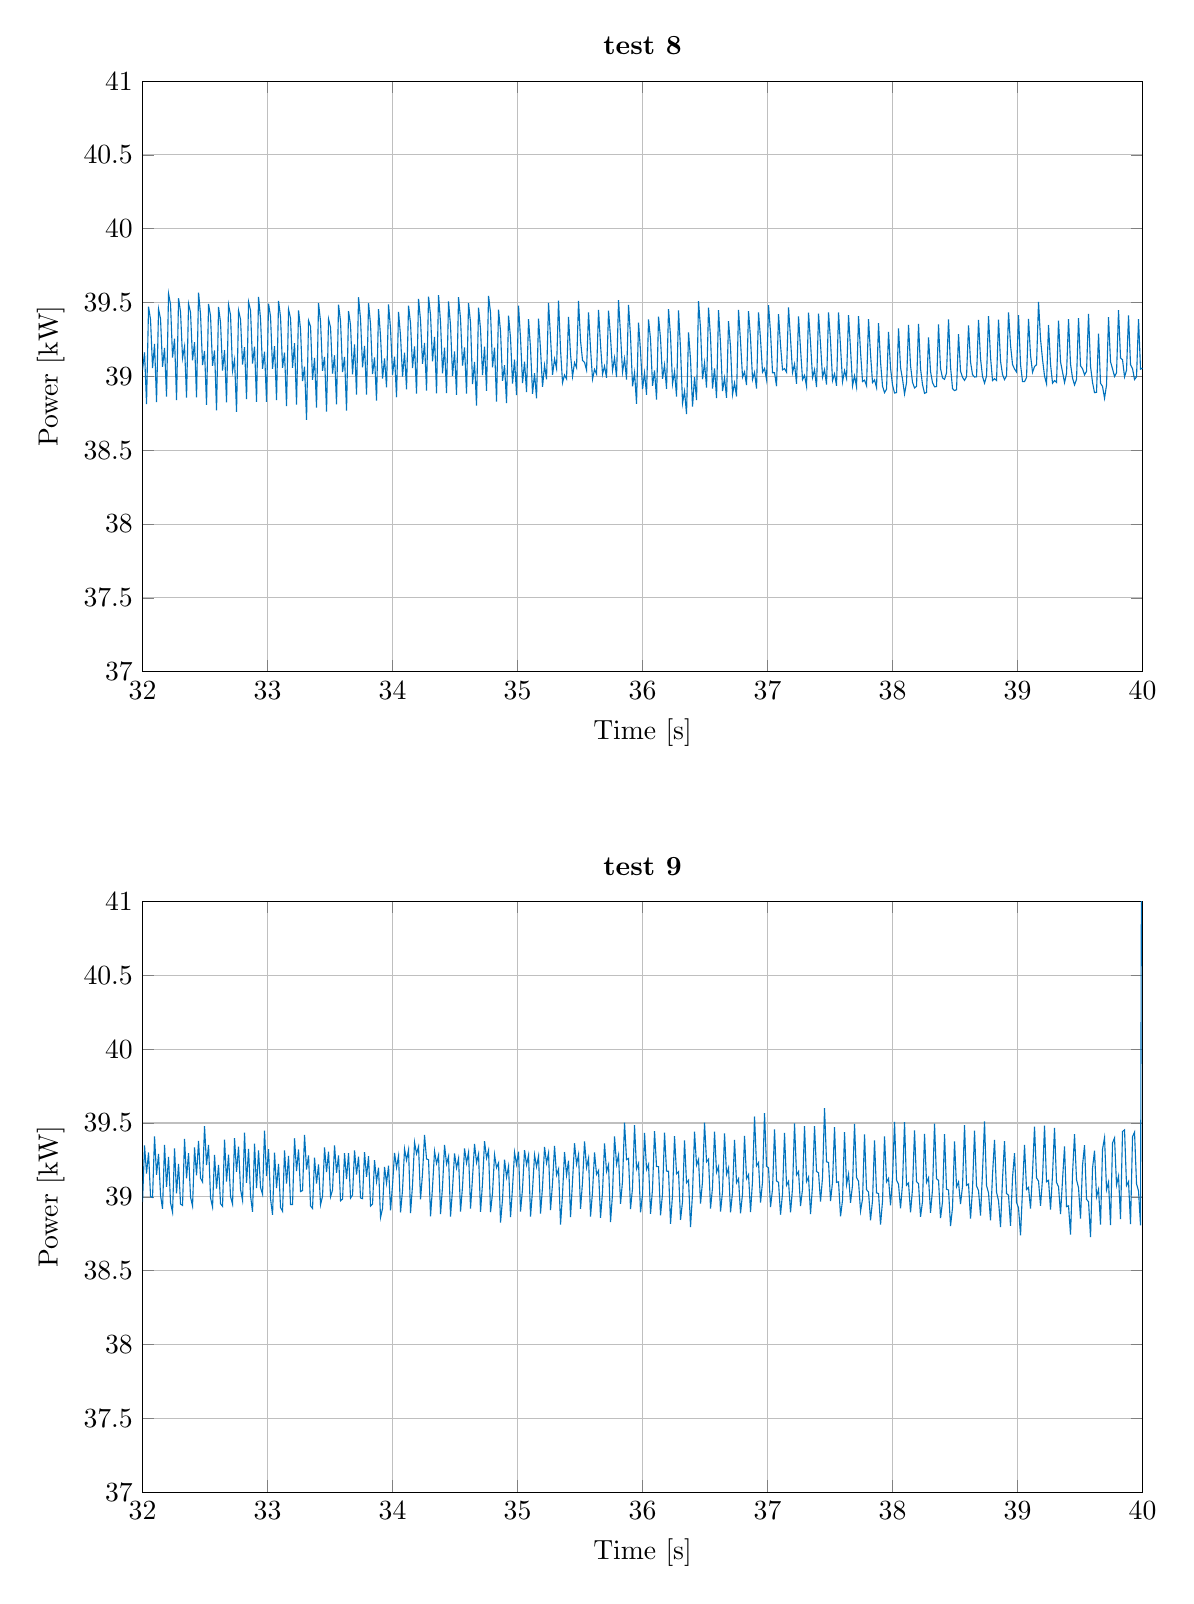
\begin{tikzpicture}

\begin{axis}[%
width=5in,
height=2.953in,
at={(1.142in,5.054in)},
scale only axis,
xmin=32,
xmax=40,
xlabel={Time [s]},
xmajorgrids,
ymin=37,
ymax=41,
ylabel={Power [kW]},
ymajorgrids,
axis background/.style={fill=white},
title style={font=\bfseries},
title={test 8}
]
\addplot [color=mycolor1,solid,forget plot]
  table[row sep=crcr]{%
32	39.0451980302526\\
32.016	39.1632046184308\\
32.032	38.8118232571152\\
32.048	39.4718399843816\\
32.064	39.38367237625\\
32.08	39.056442910818\\
32.096	39.2195689818693\\
32.112	38.8258404429622\\
32.128	39.4573455879424\\
32.144	39.3885015545951\\
32.16	39.0652761667864\\
32.176	39.1929097296981\\
32.192	38.8625798164391\\
32.208	39.5607235276013\\
32.224	39.4868809046263\\
32.24	39.1278541658036\\
32.256	39.2554381161375\\
32.272	38.8394573053181\\
32.288	39.5291121471239\\
32.304	39.436295070895\\
32.32	39.123823442348\\
32.336	39.2025253237886\\
32.352	38.8566490122056\\
32.368	39.4924135910256\\
32.384	39.4322435849582\\
32.4	39.1089022140225\\
32.416	39.232096047738\\
32.432	38.8587450738041\\
32.448	39.5673701535025\\
32.464	39.4199326362811\\
32.48	39.0770415432101\\
32.496	39.1726708480794\\
32.512	38.8075226000662\\
32.528	39.4907162671158\\
32.544	39.4087870033041\\
32.56	39.0715167300747\\
32.576	39.175260598153\\
32.592	38.7696261199989\\
32.608	39.4703861216346\\
32.624	39.3632467240091\\
32.64	39.0399526248977\\
32.656	39.1784981348184\\
32.672	38.8234040831913\\
32.688	39.4851992503692\\
32.704	39.4156344289926\\
32.72	39.0365014187217\\
32.736	39.1136110594038\\
32.752	38.7606860023692\\
32.768	39.4464606862287\\
32.784	39.3859697928686\\
32.8	39.0800021259261\\
32.816	39.1982685123412\\
32.832	38.8455323043895\\
32.848	39.5053958929572\\
32.864	39.4467238429125\\
32.88	39.0868239466889\\
32.896	39.201129400907\\
32.912	38.8270704530438\\
32.928	39.538651844083\\
32.944	39.3887975337745\\
32.96	39.0513264046246\\
32.976	39.1669267615739\\
32.992	38.828192739303\\
33.008	39.4930670341389\\
33.024	39.4051312909491\\
33.04	39.0507138539846\\
33.056	39.2046867634513\\
33.072	38.8387371015661\\
33.088	39.5117817230684\\
33.104	39.4011659741733\\
33.12	39.0585808646446\\
33.136	39.1614543844126\\
33.152	38.7982577993152\\
33.168	39.4548318673347\\
33.184	39.3927337137812\\
33.2	39.0584077553891\\
33.216	39.2248214587328\\
33.232	38.8097247001341\\
33.248	39.4474217179122\\
33.264	39.3191915093587\\
33.28	38.9680237975396\\
33.296	39.0652272746199\\
33.312	38.7055660790294\\
33.328	39.3784470592545\\
33.344	39.3382657892205\\
33.36	38.9765929285517\\
33.376	39.125071693116\\
33.392	38.7880755779163\\
33.408	39.4955775656971\\
33.424	39.3728025586653\\
33.44	39.0384161744766\\
33.456	39.1325569880429\\
33.472	38.762308894789\\
33.488	39.3886646883062\\
33.504	39.3316558693696\\
33.52	39.018336354294\\
33.536	39.1429694958917\\
33.552	38.8100678722954\\
33.568	39.4853383342215\\
33.584	39.3742083706927\\
33.6	39.0286779726247\\
33.616	39.1322517393259\\
33.632	38.7681325033283\\
33.648	39.4426749470323\\
33.664	39.3462400668469\\
33.68	39.0133385722726\\
33.696	39.217081138437\\
33.712	38.8759489323543\\
33.728	39.5359226010866\\
33.744	39.3881284398206\\
33.76	39.0607248632215\\
33.776	39.2060947679479\\
33.792	38.877147872121\\
33.808	39.4953030498293\\
33.824	39.3534658881931\\
33.84	39.0151797230516\\
33.856	39.1284396926798\\
33.872	38.8354959889181\\
33.888	39.4559147836803\\
33.904	39.2713998461365\\
33.92	38.9846168065506\\
33.936	39.1214681579227\\
33.952	38.9254877474105\\
33.968	39.487535168723\\
33.984	39.3224811199623\\
34	39.0114381627505\\
34.016	39.1335015259606\\
34.032	38.8589623951074\\
34.048	39.4368856420106\\
34.064	39.2733856485397\\
34.08	38.9987672879977\\
34.096	39.1610377166636\\
34.112	38.9121889250194\\
34.128	39.4797967683562\\
34.144	39.3591045945968\\
34.16	39.0565328580028\\
34.176	39.2037209408625\\
34.192	38.8835085100089\\
34.208	39.5255710199926\\
34.224	39.3789153810946\\
34.24	39.0854587830797\\
34.256	39.2267630922703\\
34.272	38.9039379445209\\
34.288	39.540119345928\\
34.304	39.4156495464115\\
34.32	39.1016090972254\\
34.336	39.2672926549658\\
34.352	38.8844692959604\\
34.368	39.5504980280663\\
34.384	39.3643477796587\\
34.4	39.0206658759243\\
34.416	39.1940908821922\\
34.432	38.8863816851158\\
34.448	39.5077371540469\\
34.464	39.3415394036762\\
34.48	39.0033828246343\\
34.496	39.1696545796701\\
34.512	38.8752158359588\\
34.528	39.5362875663799\\
34.544	39.388669057943\\
34.56	39.0725444061787\\
34.576	39.1956801517911\\
34.592	38.8827859849144\\
34.608	39.4961839937372\\
34.624	39.3640574003653\\
34.64	38.9480324634967\\
34.656	39.0973475783801\\
34.672	38.8018073334554\\
34.688	39.4659429654201\\
34.704	39.3176244852781\\
34.72	39.0091288914867\\
34.736	39.2020008232772\\
34.752	38.9020933971644\\
34.768	39.5458340076919\\
34.784	39.4314456763849\\
34.8	39.0613818050526\\
34.816	39.1953721638538\\
34.832	38.828692227137\\
34.848	39.4515033374958\\
34.864	39.3039537291085\\
34.88	38.9705039447595\\
34.896	39.0757077574943\\
34.912	38.8184324322779\\
34.928	39.4111064012248\\
34.944	39.2582679426891\\
34.96	38.9505712470489\\
34.976	39.1141819701588\\
34.992	38.8741358911268\\
35.008	39.4785448001875\\
35.024	39.2568283304706\\
35.04	38.9546784328\\
35.056	39.1003262959357\\
35.072	38.8942357312451\\
35.088	39.3876311556223\\
35.104	39.1894473889018\\
35.12	38.882594715271\\
35.136	39.0210673122091\\
35.152	38.8514049155631\\
35.168	39.3913246043826\\
35.184	39.1790323565614\\
35.2	38.9289920368388\\
35.216	39.0752110674614\\
35.232	38.9804163681939\\
35.248	39.498388913468\\
35.264	39.2610659505223\\
35.28	39.0113832981384\\
35.296	39.1176430688757\\
35.312	39.0537561372907\\
35.328	39.5135010398713\\
35.344	39.1806908227316\\
35.36	38.9573086028341\\
35.376	39.0100297809458\\
35.392	38.9834958560541\\
35.408	39.4027583418809\\
35.424	39.1481675339676\\
35.44	38.9993820706042\\
35.456	39.0930350318918\\
35.472	39.0591946061773\\
35.488	39.5120288697491\\
35.504	39.2421112568515\\
35.52	39.1084219719486\\
35.536	39.0947215238565\\
35.552	39.0432201231425\\
35.568	39.433448881861\\
35.584	39.1881174172487\\
35.6	38.982102697957\\
35.616	39.0477527646125\\
35.632	39.0157215438563\\
35.648	39.4506908565363\\
35.664	39.2135149107087\\
35.68	39.0147016137108\\
35.696	39.0696787464616\\
35.712	38.9907976560461\\
35.728	39.4447428165443\\
35.744	39.2642103757206\\
35.76	39.0405218462706\\
35.776	39.1257478238192\\
35.792	38.9947878345904\\
35.808	39.517094947545\\
35.824	39.2854503330872\\
35.84	39.0297214694222\\
35.856	39.1193293276997\\
35.872	38.9785462321436\\
35.888	39.4840831048188\\
35.904	39.270893721784\\
35.92	38.9326917698754\\
35.936	39.0251158585423\\
35.952	38.8148960553353\\
35.968	39.3645109500694\\
35.984	39.1693698492348\\
36	38.9146289847181\\
36.016	39.0242488357088\\
36.032	38.8754622250523\\
36.048	39.3855970251627\\
36.064	39.2502247694472\\
36.08	38.9355873272603\\
36.096	39.040864795296\\
36.112	38.8434784474967\\
36.128	39.4046303263842\\
36.144	39.2554025868477\\
36.16	38.9840669377963\\
36.176	39.0777723374896\\
36.192	38.9149769109548\\
36.208	39.4558227143768\\
36.224	39.2735869837323\\
36.24	38.9495037726953\\
36.256	39.0321635459398\\
36.272	38.8627488895537\\
36.288	39.4468472587904\\
36.304	39.1848679837487\\
36.32	38.8183087326164\\
36.336	38.8997908256134\\
36.352	38.7448495553989\\
36.368	39.2983966289033\\
36.384	39.1130170730888\\
36.4	38.7960691403935\\
36.416	38.9953975734292\\
36.432	38.8398511064553\\
36.448	39.5102938128194\\
36.464	39.3229762315647\\
36.48	38.9810405694019\\
36.496	39.0911601154476\\
36.512	38.9238694093015\\
36.528	39.4651355965429\\
36.544	39.2635557199406\\
36.56	38.9179633540605\\
36.576	39.0545175526877\\
36.592	38.8523291461611\\
36.608	39.4482284550702\\
36.624	39.2202367289822\\
36.64	38.9006418877106\\
36.656	38.9894195034851\\
36.672	38.8548759486613\\
36.688	39.3734749047262\\
36.704	39.1967903718127\\
36.72	38.8779524492292\\
36.736	38.9552799792704\\
36.752	38.8643369998112\\
36.768	39.4507992393093\\
36.784	39.2350082841265\\
36.8	38.9948325191663\\
36.816	39.0308651162553\\
36.832	38.9409367660482\\
36.848	39.4413340392444\\
36.864	39.2586852042835\\
36.88	38.9792205428884\\
36.896	39.0271467150433\\
36.912	38.9179625138856\\
36.928	39.4340789061178\\
36.944	39.2494193783691\\
36.96	39.0286096718992\\
36.976	39.0539681426828\\
36.992	38.9778072328004\\
37.008	39.4820986924404\\
37.024	39.2972084411892\\
37.04	39.0245717200405\\
37.056	39.0248218843382\\
37.072	38.9337575450029\\
37.088	39.4221097863187\\
37.104	39.2112462550638\\
37.12	39.0444984713956\\
37.136	39.0527620301017\\
37.152	39.0287426136763\\
37.168	39.4665857031113\\
37.184	39.2545824539859\\
37.2	39.0260076821261\\
37.216	39.0832502772654\\
37.232	38.9498309299612\\
37.248	39.4063724430302\\
37.264	39.184600067928\\
37.28	38.9785667990858\\
37.296	39.0074610434082\\
37.312	38.9331443414751\\
37.328	39.4317940228282\\
37.344	39.2294160230215\\
37.36	38.9919878108367\\
37.376	39.0452490590999\\
37.392	38.9275482488848\\
37.408	39.4254516634133\\
37.424	39.2156728778388\\
37.44	38.9940834174907\\
37.456	39.045871292215\\
37.472	38.9451707869983\\
37.488	39.4329059469965\\
37.504	39.2394330988595\\
37.52	38.9714278488241\\
37.536	39.0171373287227\\
37.552	38.9363372352942\\
37.568	39.4326791276548\\
37.584	39.201476906269\\
37.6	38.9643724647576\\
37.616	39.0392422676823\\
37.632	38.9862834036065\\
37.648	39.4143215006068\\
37.664	39.1850915355193\\
37.68	38.9366019568433\\
37.696	39.0040403279861\\
37.712	38.9284034725776\\
37.728	39.4074563601372\\
37.744	39.1650599687108\\
37.76	38.9654787204399\\
37.776	38.9747336733213\\
37.792	38.937126858449\\
37.808	39.3876512994926\\
37.824	39.1485080997141\\
37.84	38.9580307482252\\
37.856	38.9765874603317\\
37.872	38.9245084531716\\
37.888	39.360258338074\\
37.904	39.0977135576942\\
37.92	38.9341502289813\\
37.936	38.8902076573264\\
37.952	38.9134525944259\\
37.968	39.3010425753559\\
37.984	39.0557607004215\\
38	38.9412071213916\\
38.016	38.8871525533014\\
38.032	38.8906362921633\\
38.048	39.3258745269931\\
38.064	39.0597522183654\\
38.08	38.980766957333\\
38.096	38.8809425962707\\
38.112	38.957507249214\\
38.128	39.349156433601\\
38.144	39.0724748418601\\
38.16	38.9594375573643\\
38.176	38.9218470579157\\
38.192	38.932758066483\\
38.208	39.3561705230208\\
38.224	39.0520212492886\\
38.24	38.9433155439036\\
38.256	38.8855055097314\\
38.272	38.8911899788659\\
38.288	39.2648566434524\\
38.304	39.0337802242245\\
38.32	38.9570042907292\\
38.336	38.9294278626505\\
38.352	38.9309264000209\\
38.368	39.3515025652539\\
38.384	39.0534772028757\\
38.4	38.9899343157972\\
38.416	38.9802419782047\\
38.432	39.0233505300468\\
38.448	39.3867721467221\\
38.464	39.0646896944725\\
38.48	38.9176275308619\\
38.496	38.9040150928003\\
38.512	38.9099467516443\\
38.528	39.2857458514133\\
38.544	39.0344643157299\\
38.56	38.993700169063\\
38.576	38.9733731895227\\
38.592	38.9980371658343\\
38.608	39.3461569008342\\
38.624	39.0979492793825\\
38.64	39.0113891566155\\
38.656	38.9959719705299\\
38.672	38.9971719242942\\
38.688	39.3819370925232\\
38.704	39.118926772821\\
38.72	38.9984209914625\\
38.736	38.9543704102346\\
38.752	39.0022460421425\\
38.768	39.4074591186527\\
38.784	39.1292491383157\\
38.8	38.9720902001147\\
38.816	38.9846777954212\\
38.832	38.9729455278523\\
38.848	39.3840258688901\\
38.864	39.1031377060757\\
38.88	39.0117400652122\\
38.896	38.9783728677393\\
38.912	39.0038008297576\\
38.928	39.4340532333435\\
38.944	39.210895817394\\
38.96	39.0806879224076\\
38.976	39.050531751523\\
38.992	39.0298291352921\\
39.008	39.4149611349451\\
39.024	39.0811990405139\\
39.04	38.9648259831014\\
39.056	38.9650238979104\\
39.072	38.9931652660659\\
39.088	39.3891532537258\\
39.104	39.1431382005918\\
39.12	39.0280223214145\\
39.136	39.0662012719938\\
39.152	39.0791242404081\\
39.168	39.5041509898339\\
39.184	39.2529830445447\\
39.2	39.1146405691893\\
39.216	39.0030455203168\\
39.232	38.9497768522029\\
39.248	39.3479847507971\\
39.264	39.0827401112429\\
39.28	38.9542513829514\\
39.296	38.9718002135391\\
39.312	38.959513250495\\
39.328	39.3782532971752\\
39.344	39.0987228385343\\
39.36	39.0294861938533\\
39.376	38.9580759002984\\
39.392	39.0188664111427\\
39.408	39.3879831812032\\
39.424	39.0832281185867\\
39.44	38.98825113835\\
39.456	38.9421793286006\\
39.472	38.980228582522\\
39.488	39.3951330384167\\
39.504	39.0711595645525\\
39.52	39.052507961493\\
39.536	39.0103279146334\\
39.552	39.0343607773367\\
39.568	39.4232692977714\\
39.584	39.0682701172451\\
39.6	38.9586647901107\\
39.616	38.8900570634021\\
39.632	38.8921396739994\\
39.648	39.2903826357452\\
39.664	38.9535318183574\\
39.68	38.932127654824\\
39.696	38.8520410879615\\
39.712	38.9415327386009\\
39.728	39.400768399462\\
39.744	39.0989165454174\\
39.76	39.0509932427316\\
39.776	38.9993719073835\\
39.792	39.0242987363164\\
39.808	39.4484634444912\\
39.824	39.1245287241594\\
39.84	39.1127623305466\\
39.856	38.9965437517333\\
39.872	39.0421136762732\\
39.888	39.4134536738795\\
39.904	39.0790066179442\\
39.92	39.0523669579267\\
39.936	38.9793234086294\\
39.952	38.9973568923753\\
39.968	39.3882430171156\\
39.984	39.0488009234648\\
40	39.0556461466694\\
40	39.0556461466694\\
};
\end{axis}

\begin{axis}[%
width=5in,
height=2.953in,
at={(1.142in,0.952in)},
scale only axis,
xmin=32,
xmax=40,
xlabel={Time [s]},
xmajorgrids,
ymin=37,
ymax=41,
ylabel={Power [kW]},
ymajorgrids,
axis background/.style={fill=white},
title style={font=\bfseries},
title={test 9}
]
\addplot [color=mycolor1,solid,forget plot]
  table[row sep=crcr]{%
32	38.9649388138842\\
32.016	39.3478149353534\\
32.032	39.1579493341312\\
32.048	39.2998152158587\\
32.064	39.0018969905541\\
32.08	38.9958186155189\\
32.096	39.408599469183\\
32.112	39.1496063242254\\
32.128	39.2899324048932\\
32.144	39.0108209413874\\
32.16	38.9180430531725\\
32.176	39.352295681613\\
32.192	39.0671137021874\\
32.208	39.2699394578873\\
32.224	38.9592373235357\\
32.24	38.8951502397716\\
32.256	39.3281061273945\\
32.272	39.0231236492246\\
32.288	39.2226997717661\\
32.304	38.9506361263736\\
32.32	38.941574725211\\
32.336	39.3921274201774\\
32.352	39.1258927353942\\
32.368	39.2963506035569\\
32.384	38.9977409162322\\
32.4	38.9373667265231\\
32.416	39.3341870011793\\
32.432	39.1452264532784\\
32.448	39.3792993046615\\
32.464	39.126488735097\\
32.48	39.1005754192361\\
32.496	39.4780390949865\\
32.512	39.2145289660465\\
32.528	39.3513690553803\\
32.544	38.993184932801\\
32.56	38.9306402151506\\
32.576	39.2839713543447\\
32.592	39.0562910767107\\
32.608	39.215620760499\\
32.624	38.9531767196028\\
32.64	38.9357326904756\\
32.656	39.3874867283531\\
32.672	39.1036578997842\\
32.688	39.2857699431717\\
32.704	39.0012250690206\\
32.72	38.9507749614656\\
32.736	39.3977049830645\\
32.752	39.1691682021578\\
32.768	39.3391022188036\\
32.784	39.0503751330999\\
32.8	38.9761469018961\\
32.816	39.4341431499613\\
32.832	39.0939704405513\\
32.848	39.3240478601404\\
32.864	39.0079409675847\\
32.88	38.8981403788624\\
32.896	39.3607068001659\\
32.912	39.0583113619243\\
32.928	39.3149496381043\\
32.944	39.0628077850615\\
32.96	39.0174897013791\\
32.976	39.4484414211514\\
32.992	39.1395411794987\\
33.008	39.3234234638607\\
33.024	38.9858452909366\\
33.04	38.8777473631405\\
33.056	39.2991930802495\\
33.072	39.0596333692873\\
33.088	39.2223695731672\\
33.104	38.9279290999975\\
33.12	38.9022428233312\\
33.136	39.3141819798559\\
33.152	39.089593014698\\
33.168	39.276647298928\\
33.184	38.9480942035134\\
33.2	38.9471930119068\\
33.216	39.3964264307792\\
33.232	39.1747412759604\\
33.248	39.3201561037037\\
33.264	39.0357022987987\\
33.28	39.0427919404489\\
33.296	39.419930071823\\
33.312	39.1848255555468\\
33.328	39.2797190474734\\
33.344	38.9386188429647\\
33.36	38.9212065431305\\
33.376	39.2644085504703\\
33.392	39.0896069135907\\
33.408	39.2195048914663\\
33.424	38.9455709132277\\
33.44	39.004444788704\\
33.456	39.3342518830527\\
33.472	39.1674896998326\\
33.488	39.3053513053396\\
33.504	39.0000618556891\\
33.52	39.0462902311636\\
33.536	39.3486660284748\\
33.552	39.1618690059712\\
33.568	39.2802082763111\\
33.584	38.9731134192401\\
33.6	38.9848996099223\\
33.616	39.2948432197696\\
33.632	39.1206228413142\\
33.648	39.2950004461628\\
33.664	38.9912599318953\\
33.68	39.0123550026418\\
33.696	39.3148229241956\\
33.712	39.1508496938753\\
33.728	39.2722527556605\\
33.744	38.9918704369363\\
33.76	38.9874804799639\\
33.776	39.3029402488045\\
33.792	39.1359656626981\\
33.808	39.2754492478085\\
33.824	38.9369232178234\\
33.84	38.9506940226245\\
33.856	39.2478978534919\\
33.872	39.1032430855977\\
33.888	39.196538985422\\
33.904	38.8600024900067\\
33.92	38.9210570754267\\
33.936	39.2020716516144\\
33.952	39.0915148222211\\
33.968	39.2103314446563\\
33.984	38.9077751301358\\
34	39.0800709223784\\
34.016	39.2974748870857\\
34.032	39.1976935365851\\
34.048	39.2773908838051\\
34.064	38.894006661822\\
34.08	39.0473476110184\\
34.096	39.3240570529784\\
34.112	39.2479651723651\\
34.128	39.3191563097443\\
34.144	38.8892963710709\\
34.16	39.0799767791241\\
34.176	39.3690275435575\\
34.192	39.2917991827772\\
34.208	39.3403675983713\\
34.224	38.9820713468772\\
34.24	39.1592860810617\\
34.256	39.4185385175559\\
34.272	39.2564291902713\\
34.288	39.2502870132654\\
34.304	38.8684054093069\\
34.32	39.0662677782376\\
34.336	39.308526250109\\
34.352	39.2257899837667\\
34.368	39.2808982087321\\
34.384	38.8828433749208\\
34.4	39.069967921987\\
34.416	39.3513024741143\\
34.432	39.2225681103341\\
34.448	39.2736952531901\\
34.464	38.8666012131109\\
34.48	39.0542809060282\\
34.496	39.2937471919938\\
34.512	39.1950664880891\\
34.528	39.2603743163358\\
34.544	38.9005637611724\\
34.56	39.0699363428194\\
34.576	39.3277781753077\\
34.592	39.2282831352073\\
34.608	39.300658026777\\
34.624	38.9203137991102\\
34.64	39.1319387316763\\
34.656	39.3577358156203\\
34.672	39.2315646034171\\
34.688	39.2899985339226\\
34.704	38.8976595643518\\
34.72	39.0938615194678\\
34.736	39.3771320716261\\
34.752	39.2620955931592\\
34.768	39.3152700777917\\
34.784	38.8957153322816\\
34.8	39.0281485343472\\
34.816	39.2842709897547\\
34.832	39.1967000883455\\
34.848	39.2298103563524\\
34.864	38.825981930696\\
34.88	38.984180705467\\
34.896	39.2515060182908\\
34.912	39.1327953053819\\
34.928	39.2067056054664\\
34.944	38.8618139830938\\
34.96	39.0627846936645\\
34.976	39.3003784865174\\
34.992	39.2192667115907\\
35.008	39.3056047371528\\
35.024	38.8996435874058\\
35.04	39.0559182929306\\
35.056	39.3165534279574\\
35.072	39.2171694692406\\
35.088	39.2828785880973\\
35.104	38.8658495612541\\
35.12	39.0477933718076\\
35.136	39.2836196533511\\
35.152	39.2039061272192\\
35.168	39.2754357187813\\
35.184	38.88701078786\\
35.2	39.0685814790388\\
35.216	39.3373409128553\\
35.232	39.2281488337865\\
35.248	39.2962522920511\\
35.264	38.910187874961\\
35.28	39.0924589249569\\
35.296	39.3443305471659\\
35.312	39.1477302587834\\
35.328	39.1887992422219\\
35.344	38.8120652427089\\
35.36	39.0200043353856\\
35.376	39.3032117267674\\
35.392	39.1467929862412\\
35.408	39.2450903508192\\
35.424	38.8620719078155\\
35.44	39.1056059466705\\
35.456	39.3624726068553\\
35.472	39.2205924071762\\
35.488	39.2867315906127\\
35.504	38.9176755132678\\
35.52	39.1008391637172\\
35.536	39.375314177252\\
35.552	39.198501643341\\
35.568	39.2623134014383\\
35.584	38.8657505924264\\
35.6	39.0359982455294\\
35.616	39.2998649522546\\
35.632	39.1516301438074\\
35.648	39.177884481822\\
35.664	38.8582654833223\\
35.68	39.0357964386115\\
35.696	39.3615453482195\\
35.712	39.1708195560791\\
35.728	39.2179649651127\\
35.744	38.8290704993862\\
35.76	39.0235432753296\\
35.776	39.4092736572014\\
35.792	39.2204951314177\\
35.808	39.2834831262699\\
35.824	38.9526309939421\\
35.84	39.1068712172825\\
35.856	39.502856315989\\
35.872	39.2513876245351\\
35.888	39.2597142210155\\
35.904	38.9173761916709\\
35.92	39.0604286449774\\
35.936	39.4852724448205\\
35.952	39.1887166735141\\
35.968	39.2262170929047\\
35.984	38.894470950395\\
36	39.0163080056643\\
36.016	39.4331578321826\\
36.032	39.1851315043101\\
36.048	39.2202490528908\\
36.064	38.8848437469393\\
36.08	39.0535563017823\\
36.096	39.4450112526471\\
36.112	39.2052137741154\\
36.128	39.2040332793435\\
36.144	38.8743821066761\\
36.16	39.0245173660553\\
36.176	39.434746582283\\
36.192	39.1736877724483\\
36.208	39.1730281489899\\
36.224	38.8168300144123\\
36.24	39.0151222613307\\
36.256	39.4102108908353\\
36.272	39.1559243876702\\
36.288	39.1705802830299\\
36.304	38.8432823054741\\
36.32	38.9703641095455\\
36.336	39.3816422583354\\
36.352	39.0949340048432\\
36.368	39.1130900594917\\
36.384	38.7955029141292\\
36.4	39.0238417046418\\
36.416	39.4417059838493\\
36.432	39.2148059326319\\
36.448	39.2535046513055\\
36.464	38.9539205178687\\
36.48	39.1060848454097\\
36.496	39.503014856602\\
36.512	39.2366562449671\\
36.528	39.2552612849354\\
36.544	38.9206301081895\\
36.56	39.0641461317945\\
36.576	39.4412961789529\\
36.592	39.1655606886859\\
36.608	39.2057855080075\\
36.624	38.8992709391927\\
36.64	39.0364143075562\\
36.656	39.4301626728936\\
36.672	39.1520024145403\\
36.688	39.1968345471612\\
36.704	38.8944081899036\\
36.72	39.0335607186537\\
36.736	39.3849917213691\\
36.752	39.0956117754976\\
36.768	39.1230877300856\\
36.784	38.8886062194389\\
36.8	39.0215340698365\\
36.816	39.4124270960838\\
36.832	39.122958375444\\
36.848	39.1506503350985\\
36.864	38.8965082074307\\
36.88	39.1070831086397\\
36.896	39.543768993269\\
36.912	39.2097307032167\\
36.928	39.2326684547847\\
36.944	38.9605692805146\\
36.96	39.1018030123611\\
36.976	39.5662429974475\\
36.992	39.2070736362872\\
37.008	39.1959636500123\\
37.024	38.9309987233908\\
37.04	39.052694992927\\
37.056	39.4570627755362\\
37.072	39.1075809923716\\
37.088	39.0979850273787\\
37.104	38.8787739590564\\
37.12	39.0238026368143\\
37.136	39.4334493524\\
37.152	39.0779006989423\\
37.168	39.1048389534519\\
37.184	38.8941204124103\\
37.2	39.0572479011976\\
37.216	39.4964792891498\\
37.232	39.148506812924\\
37.248	39.1720879765262\\
37.264	38.9376529369381\\
37.28	39.0517524890223\\
37.296	39.4777896424243\\
37.312	39.1032583997225\\
37.328	39.1340147533883\\
37.344	38.8832701017188\\
37.36	39.0774466623412\\
37.376	39.4786334635074\\
37.392	39.1712272975028\\
37.408	39.1623700789468\\
37.424	38.9675612329634\\
37.44	39.1308531516356\\
37.456	39.5996777803172\\
37.472	39.237270717796\\
37.488	39.2322131564479\\
37.504	38.9705881527828\\
37.52	39.1008023289414\\
37.536	39.4711957615484\\
37.552	39.0974818982535\\
37.568	39.101491390373\\
37.584	38.8673808297108\\
37.6	38.97751326023\\
37.616	39.4377042589164\\
37.632	39.0818622918736\\
37.648	39.1534575348177\\
37.664	38.9590840824064\\
37.68	39.0802228300161\\
37.696	39.4930312279914\\
37.712	39.130801244538\\
37.728	39.1052772193821\\
37.744	38.9026748247062\\
37.76	38.9844193277438\\
37.776	39.4234326971007\\
37.792	39.0483561128615\\
37.808	39.0320486844575\\
37.824	38.8411118046044\\
37.84	38.9759228776794\\
37.856	39.381410995001\\
37.872	39.0265907205796\\
37.888	39.0223075005484\\
37.904	38.8115474904337\\
37.92	38.9721484645662\\
37.936	39.4091197045368\\
37.952	39.1012882364133\\
37.968	39.1250246010464\\
37.984	38.943007399233\\
38	39.1273790804677\\
38.016	39.507351281645\\
38.032	39.1135685561877\\
38.048	39.0843480519909\\
38.064	38.9216271057535\\
38.08	39.086581966815\\
38.096	39.5061386933732\\
38.112	39.0781893393313\\
38.128	39.0933447291703\\
38.144	38.8941961694057\\
38.16	39.0544164499835\\
38.176	39.4500693210112\\
38.192	39.1026350066535\\
38.208	39.0891287021708\\
38.224	38.8645169279856\\
38.24	38.9699816625078\\
38.256	39.4263307161111\\
38.272	39.0974376282704\\
38.288	39.1295109454966\\
38.304	38.8912282574507\\
38.32	39.0512140625304\\
38.336	39.4960306238185\\
38.352	39.1225278052564\\
38.368	39.1109791035716\\
38.384	38.855345415367\\
38.4	38.9671175741671\\
38.416	39.4242273306219\\
38.432	39.051159521356\\
38.448	39.0458018241945\\
38.464	38.8011299776048\\
38.48	38.9273110505972\\
38.496	39.3760744516835\\
38.512	39.0669685368282\\
38.528	39.1002227915414\\
38.544	38.950541195292\\
38.56	39.0737295873657\\
38.576	39.4848913759824\\
38.592	39.0771901601851\\
38.608	39.0862544891234\\
38.624	38.8516870370445\\
38.64	39.0544196984185\\
38.656	39.4480900069353\\
38.672	39.0734915903905\\
38.688	39.0416034934725\\
38.704	38.8734662921811\\
38.72	39.1703887237457\\
38.736	39.5100874143985\\
38.752	39.0761781705177\\
38.768	39.0260651293046\\
38.784	38.8403308073696\\
38.8	39.1518334444788\\
38.816	39.384999744163\\
38.832	39.0317239832214\\
38.848	38.9728478887997\\
38.864	38.7950902749136\\
38.88	39.1213868747858\\
38.896	39.3773071725362\\
38.912	39.022069583374\\
38.928	39.010801457452\\
38.944	38.8033123198313\\
38.96	39.1307844541562\\
38.976	39.2948422965413\\
38.992	38.9622738065031\\
39.008	38.9245165062045\\
39.024	38.7397610347955\\
39.04	39.0488836886469\\
39.056	39.3521479598864\\
39.072	39.0498704537381\\
39.088	39.0633271137825\\
39.104	38.9206268408156\\
39.12	39.1642362578513\\
39.136	39.4748629219472\\
39.152	39.1278521579992\\
39.168	39.1061413793412\\
39.184	38.9393893947072\\
39.2	39.1230978910786\\
39.216	39.4811786672818\\
39.232	39.1019837950852\\
39.248	39.1113482040808\\
39.264	38.9129919047101\\
39.28	39.1505572714593\\
39.296	39.4663859813643\\
39.312	39.0975545192508\\
39.328	39.0677319715964\\
39.344	38.8829972523085\\
39.36	39.1138556668526\\
39.376	39.3411298484049\\
39.392	38.9333357957815\\
39.408	38.9386411958427\\
39.424	38.7442107333102\\
39.44	39.1558305120007\\
39.456	39.4237816419746\\
39.472	39.115597363651\\
39.488	39.0615135078896\\
39.504	38.8521572236979\\
39.52	39.2122298498239\\
39.536	39.3495827881152\\
39.552	38.9828825747652\\
39.568	38.9667788337032\\
39.584	38.7277487547338\\
39.6	39.1933860590347\\
39.616	39.3120530976057\\
39.632	38.9992183549557\\
39.648	39.0509252712297\\
39.664	38.8117180312549\\
39.68	39.3225347655057\\
39.696	39.4008078776825\\
39.712	39.047890572626\\
39.728	39.099826706243\\
39.744	38.808251381803\\
39.76	39.3647439246081\\
39.776	39.3986144509373\\
39.792	39.0800695299027\\
39.808	39.1402593376835\\
39.824	38.8489415902989\\
39.84	39.4422042137824\\
39.856	39.4532213914578\\
39.872	39.0762193868276\\
39.888	39.1031478876923\\
39.904	38.814805220443\\
39.92	39.4069031816318\\
39.936	39.4376244109237\\
39.952	39.0880959943518\\
39.968	39.039248112493\\
39.984	38.8064377604335\\
39.9918395303958	41.4\\
};
\end{axis}
\end{tikzpicture}%
% \caption{Steady state power output of the genset at 40 kW load.}
% \label{fig:test8-9steadypower40kw}
% \end{figure}

% \begin{figure}[H]
% \centering
% % This file was created by matlab2tikz.
%
%The latest updates can be retrieved from
%  http://www.mathworks.com/matlabcentral/fileexchange/22022-matlab2tikz-matlab2tikz
%where you can also make suggestions and rate matlab2tikz.
%
\definecolor{mycolor1}{rgb}{0.00000,0.44700,0.74100}%
%
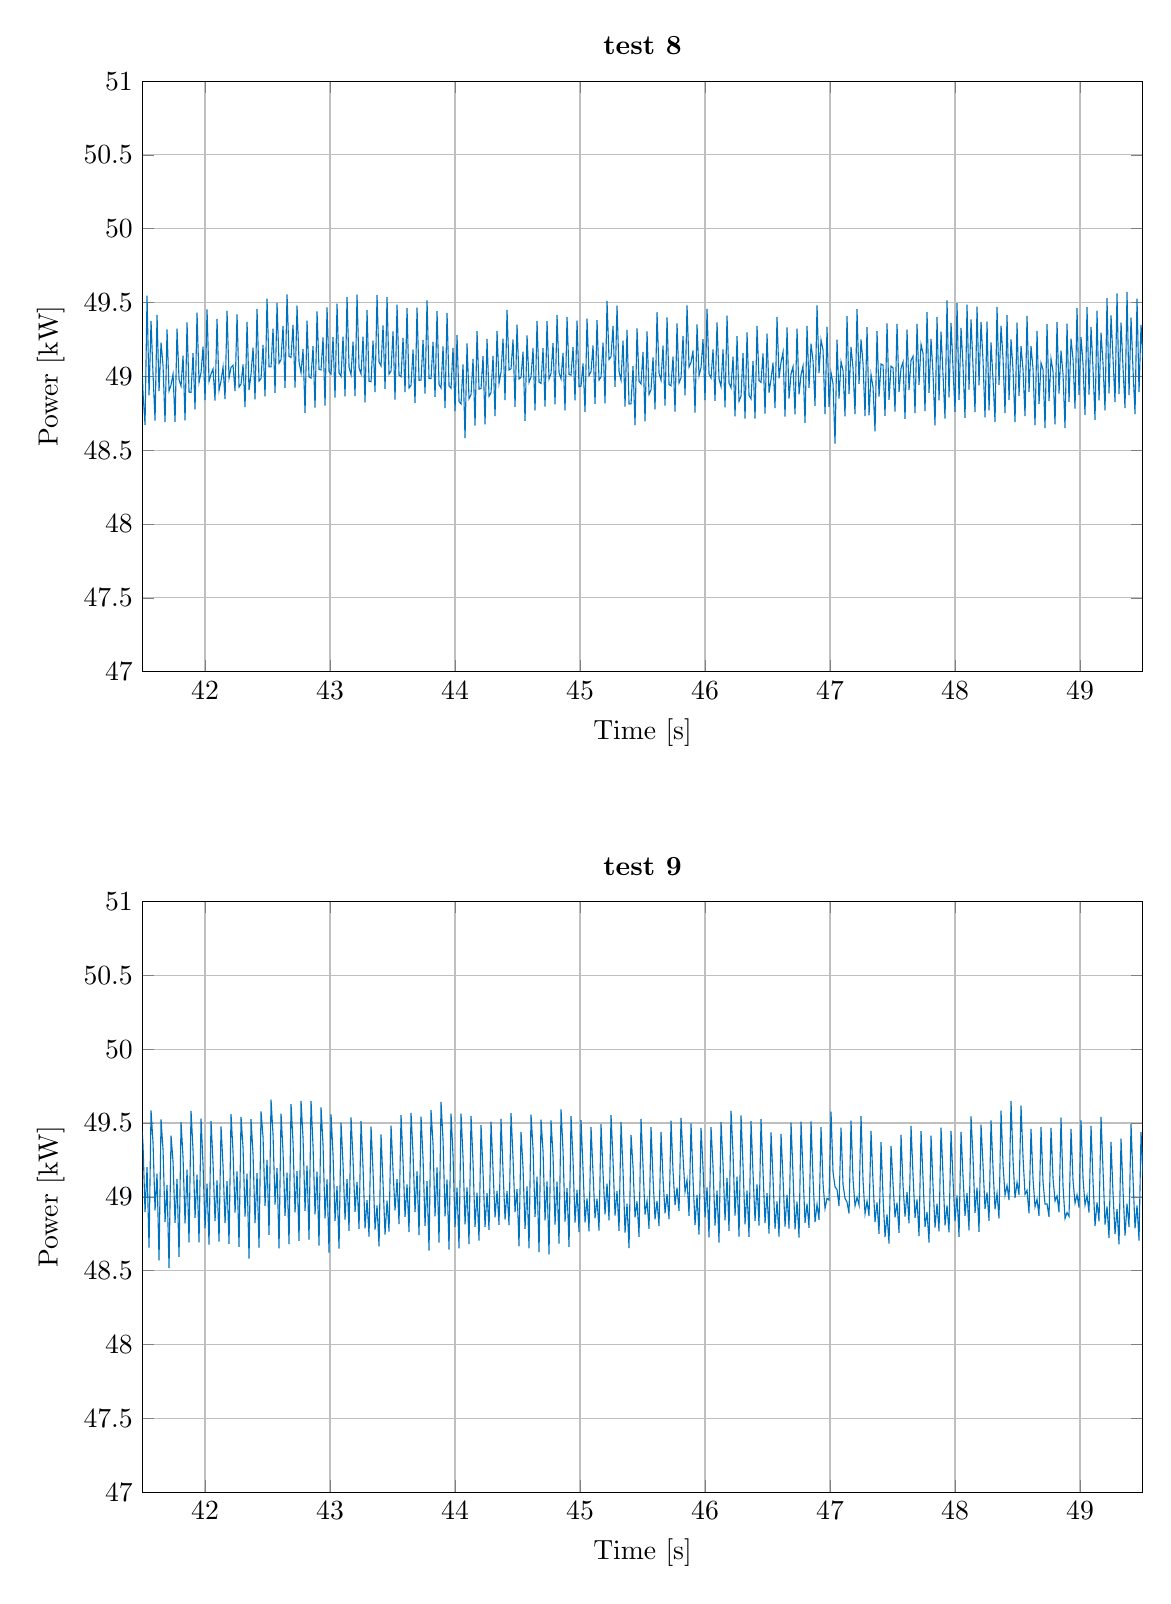
\begin{tikzpicture}

\begin{axis}[%
width=5in,
height=2.953in,
at={(1.142in,5.054in)},
scale only axis,
xmin=41.5,
xmax=49.5,
xlabel={Time [s]},
xmajorgrids,
ymin=47,
ymax=51,
ylabel={Power [kW]},
ymajorgrids,
axis background/.style={fill=white},
title style={font=\bfseries},
title={test 8}
]
\addplot [color=mycolor1,solid,forget plot]
  table[row sep=crcr]{%
41.488	49.2356620121912\\
41.504	48.884755453913\\
41.52	48.6716472869057\\
41.536	49.5464026288743\\
41.552	48.8721617063946\\
41.568	49.3753181461739\\
41.584	49.0115874283828\\
41.6	48.7008941079675\\
41.616	49.4165211524875\\
41.632	48.8999179760452\\
41.648	49.2287738383106\\
41.664	49.0724608635199\\
41.68	48.6899391939282\\
41.696	49.3179885203791\\
41.712	48.9017468328818\\
41.728	48.9424984434456\\
41.744	49.0152460500126\\
41.76	48.692849215118\\
41.776	49.3241100201983\\
41.792	48.9783964447865\\
41.808	48.9344032297057\\
41.824	49.1401915033668\\
41.84	48.7018401623785\\
41.856	49.3662489101383\\
41.872	48.893595896562\\
41.888	48.8921315167007\\
41.904	49.1568101048654\\
41.92	48.776492688748\\
41.936	49.4314043659678\\
41.952	48.9596894408704\\
41.968	49.0265059654831\\
41.984	49.2020639084303\\
42	48.8390631088736\\
42.016	49.4536651493048\\
42.032	48.9660751009307\\
42.048	49.0163533980249\\
42.064	49.0505184612856\\
42.08	48.835930340501\\
42.096	49.3888023417642\\
42.112	48.9054676056902\\
42.128	48.9698557859391\\
42.144	49.0640991102677\\
42.16	48.8468138204933\\
42.176	49.4436263989268\\
42.192	48.9890835971507\\
42.208	49.0609949458161\\
42.224	49.0743663181223\\
42.24	48.8998156700772\\
42.256	49.42053106804\\
42.272	48.9270616416261\\
42.288	48.9477390516098\\
42.304	49.080480075535\\
42.32	48.7924157602473\\
42.336	49.3687076167259\\
42.352	48.9066994504617\\
42.368	49.0163498284249\\
42.384	49.1951441980053\\
42.4	48.8439541869268\\
42.416	49.4566588768984\\
42.432	48.9676669766432\\
42.448	48.9856884969546\\
42.464	49.2131667673939\\
42.48	48.8642407773787\\
42.496	49.5269718940021\\
42.512	49.0641461334\\
42.528	49.0645425919189\\
42.544	49.3241601666553\\
42.56	48.8879870122295\\
42.576	49.4971263998248\\
42.592	49.0883035137789\\
42.608	49.1136687369989\\
42.624	49.3418005150465\\
42.64	48.9219439328937\\
42.656	49.5555416114942\\
42.672	49.1358598118479\\
42.688	49.128789909083\\
42.704	49.3484951658037\\
42.72	48.9233470178237\\
42.736	49.4790714418304\\
42.752	49.099001345662\\
42.768	49.0239017830836\\
42.784	49.1860185880314\\
42.8	48.7534271757457\\
42.816	49.3773736652886\\
42.832	48.9970954566997\\
42.848	48.9884944389814\\
42.864	49.2044909803122\\
42.88	48.7882178968533\\
42.896	49.4400676051907\\
42.912	49.0472459872329\\
42.928	49.043807655802\\
42.944	49.263641511143\\
42.96	48.801528390199\\
42.976	49.4670940680564\\
42.992	49.0342031259418\\
43.008	49.0165846309249\\
43.024	49.2659314153158\\
43.04	48.8556968027006\\
43.056	49.4921493302575\\
43.072	49.0246386552945\\
43.088	48.999994266043\\
43.104	49.2698366379233\\
43.12	48.8648466738456\\
43.136	49.5387830091633\\
43.152	49.0624586109053\\
43.168	49.0105857952898\\
43.184	49.235008582202\\
43.2	48.8663030973642\\
43.216	49.5542946818206\\
43.232	49.0570765320625\\
43.248	49.015930655658\\
43.264	49.2691478039158\\
43.28	48.8247432249403\\
43.296	49.4480972075606\\
43.312	48.9672648019118\\
43.328	48.9642784975336\\
43.344	49.2427533272826\\
43.36	48.8932983409518\\
43.376	49.550579218124\\
43.392	49.0977445940511\\
43.408	49.0722708769557\\
43.424	49.3460377094535\\
43.44	48.9158262195222\\
43.456	49.5360206724756\\
43.472	49.0150646194511\\
43.488	49.0363430381735\\
43.504	49.3055603546791\\
43.52	48.842543966781\\
43.536	49.4862985849665\\
43.552	49.0087620117522\\
43.568	48.9978558763159\\
43.584	49.2601267729373\\
43.6	48.8942952662208\\
43.616	49.4629514836975\\
43.632	48.9208940821699\\
43.648	48.9397841684259\\
43.664	49.180610369244\\
43.68	48.8186003387076\\
43.696	49.4656029549134\\
43.712	48.9739526675067\\
43.728	48.9751944718889\\
43.744	49.247305741729\\
43.76	48.882888202623\\
43.776	49.5140593288761\\
43.792	48.9857045770112\\
43.808	48.9851969534194\\
43.824	49.2336647291871\\
43.84	48.8617891012723\\
43.856	49.4414316253247\\
43.872	48.945019615842\\
43.888	48.9214421869176\\
43.904	49.2024732195837\\
43.92	48.7852622067658\\
43.936	49.430863693936\\
43.952	48.9359999204342\\
43.968	48.9202913324807\\
43.984	49.1937226403205\\
44	48.7644809377203\\
44.016	49.2791959599739\\
44.032	48.8299049396776\\
44.048	48.8132612553295\\
44.064	49.0809682826835\\
44.08	48.5815243049966\\
44.096	49.2236512672637\\
44.112	48.848018990726\\
44.128	48.87722424805\\
44.144	49.1180322831645\\
44.16	48.6660473529711\\
44.176	49.3058871318084\\
44.192	48.9139879819688\\
44.208	48.918248749063\\
44.224	49.1373818880353\\
44.24	48.675148942913\\
44.256	49.2538225527775\\
44.272	48.8654179010894\\
44.288	48.8899215759045\\
44.304	49.1387015049762\\
44.32	48.7309113314651\\
44.336	49.3079440097249\\
44.352	48.9526263094437\\
44.368	49.0284608673053\\
44.384	49.25573863327\\
44.4	48.8392870009796\\
44.416	49.4498063657707\\
44.432	49.043219806269\\
44.448	49.0517358385083\\
44.464	49.2497306579646\\
44.48	48.7945001313666\\
44.496	49.3506919530967\\
44.512	48.9814883807547\\
44.528	48.9940983413288\\
44.544	49.1677297844195\\
44.56	48.6992142156384\\
44.576	49.2784615053882\\
44.592	48.9597369371352\\
44.608	48.996680151104\\
44.624	49.1904633081415\\
44.64	48.7691952622963\\
44.656	49.3751043634586\\
44.672	48.96123383504\\
44.688	48.9529573682926\\
44.704	49.1905818967403\\
44.72	48.794801282477\\
44.736	49.3738218799211\\
44.752	48.9822066882006\\
44.768	49.0216674555404\\
44.784	49.2258098303252\\
44.8	48.8102142698029\\
44.816	49.4160579302206\\
44.832	49.0254941213589\\
44.848	48.9834021977387\\
44.864	49.1593179627309\\
44.88	48.7700621534103\\
44.896	49.4037611410063\\
44.912	49.0132372690283\\
44.928	49.0087135943663\\
44.944	49.1973109922723\\
44.96	48.8373060786198\\
44.976	49.3775384484508\\
44.992	48.9304402434187\\
45.008	48.9356458039511\\
45.024	49.088129263759\\
45.04	48.7597345514574\\
45.056	49.3906053006821\\
45.072	49.006274147797\\
45.088	49.0325852294116\\
45.104	49.2090683097021\\
45.12	48.8138375438802\\
45.136	49.3803359217482\\
45.152	48.9749414975353\\
45.168	48.9968867178247\\
45.184	49.2284757029726\\
45.2	48.8177844366102\\
45.216	49.5106856019536\\
45.232	49.114278156462\\
45.248	49.1340756633452\\
45.264	49.3412569113118\\
45.28	48.9291296102784\\
45.296	49.4789763591985\\
45.312	49.0342656682749\\
45.328	48.9744839111315\\
45.344	49.2426861983036\\
45.36	48.7957637484823\\
45.376	49.3153107885281\\
45.392	48.8131919812911\\
45.408	48.8147859740322\\
45.424	49.0689346190097\\
45.44	48.6706695291464\\
45.456	49.3253870202836\\
45.472	48.9669702650579\\
45.488	48.9489287487386\\
45.504	49.1656844234558\\
45.52	48.6963633663961\\
45.536	49.3041972658403\\
45.552	48.8784634370428\\
45.568	48.9105193702386\\
45.584	49.1292120705067\\
45.6	48.7775557998382\\
45.616	49.4344014661522\\
45.632	49.0227450659685\\
45.648	48.9742564107743\\
45.664	49.2081337161635\\
45.68	48.8016333765018\\
45.696	49.4002251019979\\
45.712	48.9446620647028\\
45.728	48.9366998775343\\
45.744	49.1341556837515\\
45.76	48.7620788355084\\
45.776	49.359257705588\\
45.792	48.9553058384607\\
45.808	48.9909024853776\\
45.824	49.2751436180121\\
45.84	48.8714388992208\\
45.856	49.4810669776286\\
45.872	49.0633742347797\\
45.888	49.0956210716599\\
45.904	49.1759351319458\\
45.92	48.7546759541267\\
45.936	49.3527741933167\\
45.952	49.0043583662989\\
45.968	49.0593213874757\\
45.984	49.2529790303766\\
46	48.8398984942478\\
46.016	49.4574693441969\\
46.032	49.0157667045658\\
46.048	48.9887450961836\\
46.064	49.1829983098234\\
46.08	48.8351641075905\\
46.096	49.3658982638666\\
46.112	48.9831882454037\\
46.128	48.9309531339052\\
46.144	49.1828185641509\\
46.16	48.7897512247037\\
46.176	49.4116129149889\\
46.192	48.9550142697707\\
46.208	48.9225401120326\\
46.224	49.1333071194138\\
46.24	48.7285661922164\\
46.256	49.2731416203479\\
46.272	48.8312176342139\\
46.288	48.8676970243839\\
46.304	49.1577693898884\\
46.32	48.7141561993386\\
46.336	49.2978063338712\\
46.352	48.870705732158\\
46.368	48.8481168289248\\
46.384	49.1048584683708\\
46.4	48.7144809275162\\
46.416	49.3421942401134\\
46.432	48.971576961489\\
46.448	48.9600341678332\\
46.464	49.1560192717663\\
46.48	48.7481047734117\\
46.496	49.2888650628795\\
46.512	48.889794479366\\
46.528	48.9802018998897\\
46.544	49.0926380418961\\
46.56	48.78536447791\\
46.576	49.4035806924744\\
46.592	48.9871602716201\\
46.608	49.0968237592759\\
46.624	49.1658891086136\\
46.64	48.7278026050166\\
46.656	49.3326504699207\\
46.672	48.8491054126753\\
46.688	49.0176138546169\\
46.704	49.0664674560828\\
46.72	48.7431094662341\\
46.736	49.3233845380983\\
46.752	48.8791976670641\\
46.768	49.0103298155604\\
46.784	49.0710990063399\\
46.8	48.6852122586716\\
46.816	49.3417265767145\\
46.832	48.9222136313188\\
46.848	49.2214448293398\\
46.864	49.1055088466126\\
46.88	48.8008401510497\\
46.896	49.4817854467714\\
46.912	49.0217605836722\\
46.928	49.2477614690213\\
46.944	49.1801119109307\\
46.96	48.7444836955509\\
46.976	49.3358510655681\\
46.992	48.7938005042793\\
47.008	49.0259554616583\\
47.024	48.9514235919265\\
47.04	48.5454384893041\\
47.056	49.2487361560496\\
47.072	48.8500788915347\\
47.088	49.0997588049811\\
47.104	49.0400392235215\\
47.12	48.7292076814082\\
47.136	49.4076420963086\\
47.152	48.8822104508492\\
47.168	49.1989740974152\\
47.184	49.0566612322832\\
47.2	48.7439494515764\\
47.216	49.4551486202992\\
47.232	48.9496052379402\\
47.248	49.2508684732967\\
47.264	49.0878117004657\\
47.28	48.731331486523\\
47.296	49.3341166110806\\
47.312	48.7361895816812\\
47.328	49.0125978104855\\
47.344	48.9267795347478\\
47.36	48.6283668228101\\
47.376	49.3069327135338\\
47.392	48.8630955442872\\
47.408	49.083851548161\\
47.424	49.0762500291225\\
47.44	48.7326125840164\\
47.456	49.3592476671357\\
47.472	48.8408648632433\\
47.488	49.0698836961032\\
47.504	49.0567090700218\\
47.52	48.7615238247595\\
47.536	49.3564105120474\\
47.552	48.8950018625465\\
47.568	49.0559293243195\\
47.584	49.0978069140405\\
47.6	48.7116701449277\\
47.616	49.3161797988624\\
47.632	48.9071621689616\\
47.648	49.1091547186421\\
47.664	49.1356034456781\\
47.68	48.7521892171417\\
47.696	49.3554749522428\\
47.712	48.9425663258875\\
47.728	49.2178149940632\\
47.744	49.1567238475922\\
47.76	48.764956599627\\
47.776	49.4353680052722\\
47.792	48.8888912838792\\
47.808	49.2539198080322\\
47.824	49.015573463877\\
47.84	48.6685647147629\\
47.856	49.4027310101625\\
47.872	48.837403636265\\
47.888	49.302563233284\\
47.904	49.0094074196301\\
47.92	48.7142890252157\\
47.936	49.5144867580038\\
47.952	48.8587260087892\\
47.968	49.3621480830128\\
47.984	49.0560503395021\\
48	48.7604512950637\\
48.016	49.4960076168055\\
48.032	48.8413847474755\\
48.048	49.3291821932552\\
48.064	49.0701537212376\\
48.08	48.7186636452093\\
48.096	49.4860105905734\\
48.112	48.9110066917872\\
48.128	49.3856807899233\\
48.144	49.0642147961713\\
48.16	48.7588578144925\\
48.176	49.473313794534\\
48.192	48.9392266847642\\
48.208	49.3692769768767\\
48.224	49.1060694186518\\
48.24	48.7228780636476\\
48.256	49.3715645137489\\
48.272	48.7701273681946\\
48.288	49.2297996167113\\
48.304	48.9779015710385\\
48.32	48.6926492523419\\
48.336	49.4715564197516\\
48.352	48.9422299024608\\
48.368	49.3423750734973\\
48.384	49.1198869699251\\
48.4	48.7517570374966\\
48.416	49.4150945380577\\
48.432	48.8396642850722\\
48.448	49.2499267130865\\
48.464	49.0431449403544\\
48.48	48.6909589820478\\
48.496	49.3639707954781\\
48.512	48.8677282973066\\
48.528	49.2052136213193\\
48.544	49.0468051116225\\
48.56	48.7311924004342\\
48.576	49.4097800960969\\
48.592	48.8955178745778\\
48.608	49.2050628535822\\
48.624	49.0495447982058\\
48.64	48.6699032945289\\
48.656	49.3078745284013\\
48.672	48.8116927452151\\
48.688	49.0921788369184\\
48.704	49.0457565657913\\
48.72	48.6490945407826\\
48.736	49.3533413514596\\
48.752	48.8326777604256\\
48.768	49.1190457502621\\
48.784	49.0336139696065\\
48.8	48.674955068795\\
48.816	49.3673327856189\\
48.832	48.8835972083382\\
48.848	49.1740814537662\\
48.864	49.0150271132775\\
48.88	48.6497717035045\\
48.896	49.3571471658658\\
48.912	48.8270706929029\\
48.928	49.2553398715647\\
48.944	49.1156684105257\\
48.96	48.7819359992293\\
48.976	49.4617595399204\\
48.992	48.8756524702109\\
49.008	49.2655393861708\\
49.024	49.0826794472143\\
49.04	48.7401892557983\\
49.056	49.4686852532553\\
49.072	48.8771192648667\\
49.088	49.3340767937626\\
49.104	49.0514669736441\\
49.12	48.7056842045561\\
49.136	49.4445907106698\\
49.152	48.837587602549\\
49.168	49.2956690310819\\
49.184	49.0875186197251\\
49.2	48.7698407884824\\
49.216	49.5297335614168\\
49.232	48.8846487050858\\
49.248	49.4129997934431\\
49.264	49.119281462958\\
49.28	48.8262670754567\\
49.296	49.5616561537861\\
49.312	48.8808466419503\\
49.328	49.3646613878558\\
49.344	49.0608434708526\\
49.36	48.7846908837615\\
49.376	49.5717594667688\\
49.392	48.8730864559491\\
49.408	49.3979296926666\\
49.424	49.0441213414509\\
49.44	48.7448108658888\\
49.456	49.5260421446826\\
49.472	48.8938383269303\\
49.488	49.3493372471847\\
49.504	49.0987882995954\\
};
\end{axis}

\begin{axis}[%
width=5in,
height=2.953in,
at={(1.142in,0.952in)},
scale only axis,
xmin=41.5,
xmax=49.5,
xlabel={Time [s]},
xmajorgrids,
ymin=47,
ymax=51,
ylabel={Power [kW]},
ymajorgrids,
axis background/.style={fill=white},
title style={font=\bfseries},
title={test 9}
]
\addplot [color=mycolor1,solid,forget plot]
  table[row sep=crcr]{%
41.488	49.5724476463382\\
41.504	49.3486620208636\\
41.52	48.8960338986448\\
41.536	49.2012602067504\\
41.552	48.6552406810012\\
41.568	49.5846743211034\\
41.584	49.3636555167402\\
41.6	48.9084884851888\\
41.616	49.1573816257077\\
41.632	48.5703606374812\\
41.648	49.5239056334283\\
41.664	49.3189221916061\\
41.68	48.8300805293604\\
41.696	49.0804774933847\\
41.712	48.5163421966984\\
41.728	49.4141932650679\\
41.744	49.2373594417614\\
41.76	48.8238670713629\\
41.776	49.1220139469627\\
41.792	48.592514438109\\
41.808	49.5048782138206\\
41.824	49.2668497121748\\
41.84	48.8194451809032\\
41.856	49.1842588419032\\
41.872	48.6912256504037\\
41.888	49.5816358702896\\
41.904	49.3140893232349\\
41.92	48.8571306387875\\
41.936	49.1502360060008\\
41.952	48.6914279113804\\
41.968	49.5294775056149\\
41.984	49.2152013724005\\
42	48.7863064703323\\
42.016	49.0896309063937\\
42.032	48.6761589355776\\
42.048	49.5127761782596\\
42.064	49.2260806013955\\
42.08	48.8362600088889\\
42.096	49.1109626292036\\
42.112	48.6969851492938\\
42.128	49.4771571783358\\
42.144	49.2081267244425\\
42.16	48.8213009590379\\
42.176	49.1052887861438\\
42.192	48.6815489198751\\
42.208	49.559260048204\\
42.224	49.3015917299659\\
42.24	48.893692333761\\
42.256	49.1714836630727\\
42.272	48.6603388072452\\
42.288	49.5413789075182\\
42.304	49.3325359171469\\
42.32	48.8652942996375\\
42.336	49.1569626581896\\
42.352	48.5819030545511\\
42.368	49.5258516181354\\
42.384	49.289241926112\\
42.4	48.8221369627666\\
42.416	49.1604422071285\\
42.432	48.6561790800811\\
42.448	49.5778720253221\\
42.464	49.4050591011899\\
42.48	48.9379437818563\\
42.496	49.2498837701248\\
42.512	48.7414650753076\\
42.528	49.6582205615229\\
42.544	49.4198379972598\\
42.56	48.947480105812\\
42.576	49.1946121664636\\
42.592	48.6500092990901\\
42.608	49.5637898699087\\
42.624	49.3036502941568\\
42.64	48.8710444812838\\
42.656	49.162885446979\\
42.672	48.6794639666109\\
42.688	49.6277920762048\\
42.704	49.3665443562031\\
42.72	48.8947160590192\\
42.736	49.1731569475354\\
42.752	48.7013111817017\\
42.768	49.649292588754\\
42.784	49.3991761796801\\
42.8	48.9051905065787\\
42.816	49.2115644851169\\
42.832	48.7107900502144\\
42.848	49.649598135139\\
42.864	49.3419611789445\\
42.88	48.8816487465599\\
42.896	49.1703257942903\\
42.912	48.668766625792\\
42.928	49.6060660696677\\
42.944	49.3508508187028\\
42.96	48.8541477735819\\
42.976	49.1174404901705\\
42.992	48.6215522564405\\
43.008	49.5581235190714\\
43.024	49.2839118895715\\
43.04	48.8358414660091\\
43.056	49.0723908322742\\
43.072	48.6495120710582\\
43.088	49.5018770965742\\
43.104	49.2181245259256\\
43.12	48.8451905838614\\
43.136	49.1189457607099\\
43.152	48.7689934481202\\
43.168	49.5371855972745\\
43.184	49.2501924378502\\
43.2	48.8985088311171\\
43.216	49.101288769085\\
43.232	48.7832011125868\\
43.248	49.5131194454116\\
43.264	49.2004901272515\\
43.28	48.7859751919426\\
43.296	48.9768410186462\\
43.312	48.7311557570889\\
43.328	49.4748738541629\\
43.344	49.1712167662175\\
43.36	48.7778668082443\\
43.376	48.9420424904378\\
43.392	48.664496986423\\
43.408	49.4225669553928\\
43.424	49.0916447392503\\
43.44	48.7445874431412\\
43.456	48.9734677355414\\
43.472	48.764243124937\\
43.488	49.4825142595911\\
43.504	49.178686905898\\
43.52	48.9081480363939\\
43.536	49.119691015445\\
43.552	48.8157078377747\\
43.568	49.5533741586483\\
43.584	49.2360563682386\\
43.6	48.8641851305038\\
43.616	49.0843938142098\\
43.632	48.761331672968\\
43.648	49.5675641924269\\
43.664	49.2874061665059\\
43.68	48.8965127261289\\
43.696	49.1727338453751\\
43.712	48.7406598116549\\
43.728	49.5426143245114\\
43.744	49.2589574678254\\
43.76	48.8034921264827\\
43.776	49.1057150688815\\
43.792	48.6347821277132\\
43.808	49.586752146366\\
43.824	49.3560392896069\\
43.84	48.8680400797855\\
43.856	49.1987006807025\\
43.872	48.6899065438211\\
43.888	49.6431714700514\\
43.904	49.383755736384\\
43.92	48.8675708020274\\
43.936	49.1169484088602\\
43.952	48.6430048775035\\
43.968	49.5637022251186\\
43.984	49.2776786848494\\
44	48.7953694080599\\
44.016	49.0621281056906\\
44.032	48.6502835941988\\
44.048	49.5629948064481\\
44.064	49.2661319305979\\
44.08	48.8137659795872\\
44.096	49.0641197420758\\
44.112	48.6802669385708\\
44.128	49.5486041150093\\
44.144	49.230342769039\\
44.16	48.7961131001147\\
44.176	49.0280333652775\\
44.192	48.7033812051605\\
44.208	49.4857270521006\\
44.224	49.1642963583213\\
44.24	48.7956968603842\\
44.256	49.025007379567\\
44.272	48.7754628408812\\
44.288	49.5085304839591\\
44.304	49.1843860698582\\
44.32	48.8607406910584\\
44.336	49.0396528693983\\
44.352	48.8097815406599\\
44.368	49.5271504780852\\
44.384	49.1762939659991\\
44.4	48.8465181589327\\
44.416	49.0376082934812\\
44.432	48.8087446207649\\
44.448	49.5669178681089\\
44.464	49.2585396391471\\
44.48	48.8960281809222\\
44.496	49.0523289554537\\
44.512	48.6652230706177\\
44.528	49.4397769304563\\
44.544	49.193888382553\\
44.56	48.7826741294937\\
44.576	49.0710077765166\\
44.592	48.6516855469118\\
44.608	49.5562676732269\\
44.624	49.3235823529539\\
44.64	48.8628982849767\\
44.656	49.1370850995388\\
44.672	48.625991104765\\
44.688	49.5218395850952\\
44.704	49.3088545541866\\
44.72	48.8410378350681\\
44.736	49.1040315480035\\
44.752	48.6104042525646\\
44.768	49.5178165333529\\
44.784	49.2752544241285\\
44.8	48.8116828594356\\
44.816	49.1019480423978\\
44.832	48.6834821242224\\
44.848	49.5923320486986\\
44.864	49.31198829497\\
44.88	48.8315489861808\\
44.896	49.0591646351512\\
44.912	48.6606037187555\\
44.928	49.5459848439628\\
44.944	49.2473703944996\\
44.96	48.8249170183246\\
44.976	49.0459502098311\\
44.992	48.7616026595752\\
45.008	49.5184642728767\\
45.024	49.1846435475987\\
45.04	48.8268567796677\\
45.056	48.9890355819927\\
45.072	48.7667331513075\\
45.088	49.4719922437564\\
45.104	49.1596170398338\\
45.12	48.8551263318645\\
45.136	48.9869846693649\\
45.152	48.7716246041128\\
45.168	49.4913317220563\\
45.184	49.1592086401136\\
45.2	48.8814283163892\\
45.216	49.0897589159757\\
45.232	48.8407907514929\\
45.248	49.5532188674258\\
45.264	49.2415693461735\\
45.28	48.87354277642\\
45.296	49.0387674128757\\
45.312	48.7687149199861\\
45.328	49.5063502954459\\
45.344	49.1717477089676\\
45.36	48.7581585117505\\
45.376	48.9535901163769\\
45.392	48.6520460168394\\
45.408	49.4195605686402\\
45.424	49.2007969650102\\
45.44	48.8606701870634\\
45.456	48.9695161018322\\
45.472	48.7293113561114\\
45.488	49.5279380929491\\
45.504	49.2036885620785\\
45.52	48.8793106634571\\
45.536	48.9736263224754\\
45.552	48.7838147719071\\
45.568	49.4713177029615\\
45.584	49.1251547555478\\
45.6	48.8477423113361\\
45.616	48.9728252934632\\
45.632	48.8015678650119\\
45.648	49.4398164200432\\
45.664	49.1218914638813\\
45.68	48.8886665213603\\
45.696	49.0177503680025\\
45.712	48.8489534990405\\
45.728	49.5165956531019\\
45.744	49.1742139219134\\
45.76	48.9436412625123\\
45.776	49.0622221559404\\
45.792	48.9040488393557\\
45.808	49.5338679176405\\
45.824	49.2700912969782\\
45.84	49.034497072575\\
45.856	49.1142024686166\\
45.872	48.8705080700126\\
45.888	49.4967049555105\\
45.904	49.1182809158462\\
45.92	48.8090566692675\\
45.936	49.012253047825\\
45.952	48.7434694198059\\
45.968	49.4664241652488\\
45.984	49.192099075822\\
46	48.8604500757393\\
46.016	49.0631825143598\\
46.032	48.7254922482021\\
46.048	49.4712326559439\\
46.064	49.2011947919315\\
46.08	48.8052160543232\\
46.096	49.0409775590059\\
46.112	48.6900128806151\\
46.128	49.506154156717\\
46.144	49.2175790493192\\
46.16	48.8408166983707\\
46.176	49.1280697936313\\
46.192	48.7688731025573\\
46.208	49.5822147206612\\
46.224	49.2882021898093\\
46.24	48.8726196476128\\
46.256	49.1358599917967\\
46.272	48.7307519758948\\
46.288	49.5505860478079\\
46.304	49.2094543039503\\
46.32	48.8134980268258\\
46.336	49.0418161244304\\
46.352	48.7288823624817\\
46.368	49.5125039851262\\
46.384	49.1580975739141\\
46.4	48.8365632305198\\
46.416	49.0833342734047\\
46.432	48.8045271690012\\
46.448	49.526489008261\\
46.464	49.1669711789615\\
46.48	48.8225778683765\\
46.496	49.0254529959808\\
46.512	48.7514985640797\\
46.528	49.4363482740867\\
46.544	49.120208951716\\
46.56	48.7839192353869\\
46.576	48.9691245270466\\
46.592	48.7300783894004\\
46.608	49.4266525180633\\
46.624	49.1210286711667\\
46.64	48.7983809311579\\
46.656	49.0126512354509\\
46.672	48.7842402425667\\
46.688	49.5026792096819\\
46.704	49.1450861428591\\
46.72	48.7803090311831\\
46.736	48.9675066025757\\
46.752	48.7236294905094\\
46.768	49.5085858660562\\
46.784	49.1572600060617\\
46.8	48.8236120719569\\
46.816	48.9530488167671\\
46.832	48.7904081066637\\
46.848	49.5100959237792\\
46.864	49.1242848913059\\
46.88	48.8282692412675\\
46.896	48.9485472679547\\
46.912	48.8436037565292\\
46.928	49.4715477178886\\
46.944	49.0889032067338\\
46.96	48.9206679488881\\
46.976	48.9897598668222\\
46.992	48.9779705272184\\
47.008	49.576444744657\\
47.024	49.1657706604391\\
47.04	49.0670830053801\\
47.056	49.0484049814902\\
47.072	48.9374132224829\\
47.088	49.469120517709\\
47.104	49.0812230504455\\
47.12	48.9894735640419\\
47.136	48.9635333933365\\
47.152	48.8873072944314\\
47.168	49.5157543893841\\
47.184	49.1180727481939\\
47.2	48.9389682975968\\
47.216	48.9963317270551\\
47.232	48.9449870286283\\
47.248	49.5467134811314\\
47.264	49.1111651442162\\
47.28	48.8856435480963\\
47.296	48.9696556577417\\
47.312	48.868903678831\\
47.328	49.4457595689893\\
47.344	49.1014374054149\\
47.36	48.8292909942913\\
47.376	48.9622886844993\\
47.392	48.7494023121393\\
47.408	49.3705739119015\\
47.424	49.0026819026372\\
47.44	48.7267666200624\\
47.456	48.879997991278\\
47.472	48.6835234554512\\
47.488	49.3442341324632\\
47.504	49.0872010088512\\
47.52	48.8605078380869\\
47.536	48.9607014369067\\
47.552	48.7554297329632\\
47.568	49.4198400689745\\
47.584	49.076524466412\\
47.6	48.8654519155815\\
47.616	49.0310698016562\\
47.632	48.8198655966733\\
47.648	49.480847759346\\
47.664	49.145277655446\\
47.68	48.8582362441323\\
47.696	48.9823280367398\\
47.712	48.7331669813806\\
47.728	49.4443631446523\\
47.744	49.1218996983512\\
47.76	48.7967345696328\\
47.776	48.8969709144774\\
47.792	48.690494464122\\
47.808	49.4143047122997\\
47.824	49.0742676834658\\
47.84	48.7915514734458\\
47.856	48.9531279121127\\
47.872	48.7660168792567\\
47.888	49.4688842580001\\
47.904	49.1435260542038\\
47.92	48.8059846636183\\
47.936	48.9422541156142\\
47.952	48.7587094356728\\
47.968	49.446862117591\\
47.984	49.1061978755178\\
48	48.8357830944091\\
48.016	49.0086574881728\\
48.032	48.7291238875094\\
48.048	49.4400763600915\\
48.064	49.1365835197779\\
48.08	48.8717210949799\\
48.096	49.0251790630949\\
48.112	48.7720116702217\\
48.128	49.5446901780284\\
48.144	49.2631844850208\\
48.16	48.8906943039095\\
48.176	49.0614900129976\\
48.192	48.7632063569326\\
48.208	49.4883186953155\\
48.224	49.211559291462\\
48.24	48.9185419741024\\
48.256	49.0303580002623\\
48.272	48.8379544759298\\
48.288	49.5180737700837\\
48.304	49.1930892156968\\
48.32	48.9160475105209\\
48.336	49.0229688212655\\
48.352	48.8533497728714\\
48.368	49.5831882915431\\
48.384	49.217677001403\\
48.4	49.0114079982535\\
48.416	49.0760455204777\\
48.432	48.9783580023489\\
48.448	49.6487920665936\\
48.464	49.2479809105962\\
48.48	48.9926825891134\\
48.496	49.096884027693\\
48.512	49.0139745936903\\
48.528	49.6177759399352\\
48.544	49.2678982929367\\
48.56	49.0162927575463\\
48.576	49.0433960393751\\
48.592	48.88757583567\\
48.608	49.4592737889852\\
48.624	49.1197606097342\\
48.64	48.9326470032368\\
48.656	48.9835021183369\\
48.672	48.8707733873901\\
48.688	49.4716671853684\\
48.704	49.1005151266259\\
48.72	48.9508744263611\\
48.736	48.9521258025477\\
48.752	48.8642603643262\\
48.768	49.4665246342395\\
48.784	49.124162371558\\
48.8	48.9720700477325\\
48.816	49.0062685968533\\
48.832	48.8955199778931\\
48.848	49.5354445863365\\
48.864	49.0729392284397\\
48.88	48.8534131297773\\
48.896	48.8932978251443\\
48.912	48.8677001428622\\
48.928	49.4604214048082\\
48.944	49.1079144077738\\
48.96	48.9573854711478\\
48.976	49.0128877659787\\
48.992	48.9274577369832\\
49.008	49.5173750396016\\
49.024	49.123802136758\\
49.04	48.9451467404207\\
49.056	49.0083953969398\\
49.072	48.8937780661211\\
49.088	49.481041013706\\
49.104	49.103887544239\\
49.12	48.8015528185439\\
49.136	48.9625943439134\\
49.152	48.8341323252798\\
49.168	49.5408530556118\\
49.184	49.1827115714814\\
49.2	48.812460568112\\
49.216	48.9351168692809\\
49.232	48.7199746953137\\
49.248	49.3714563545465\\
49.264	49.0213649603019\\
49.28	48.747911373813\\
49.296	48.9169248375534\\
49.312	48.6781702931818\\
49.328	49.3941952709885\\
49.344	49.0438181375931\\
49.36	48.7375345967795\\
49.376	48.9529751799975\\
49.392	48.7946779306183\\
49.408	49.4915978635314\\
49.424	49.1201822431484\\
49.44	48.7862259495321\\
49.456	48.9421840915712\\
49.472	48.70347600159\\
49.488	49.4383041862763\\
49.504	49.1378529786283\\
};
\end{axis}
\end{tikzpicture}%
% \caption{Steady state power output of the genset at 50 kW load.}
% \label{fig:test8-9steadypower50kw}
% \end{figure}

\subsubsection*{Volt}

\begin{figure}[H]
\centering
% This file was created by matlab2tikz.
%
%The latest updates can be retrieved from
%  http://www.mathworks.com/matlabcentral/fileexchange/22022-matlab2tikz-matlab2tikz
%where you can also make suggestions and rate matlab2tikz.
%
\definecolor{mycolor1}{rgb}{0.00000,0.44700,0.74100}%
%
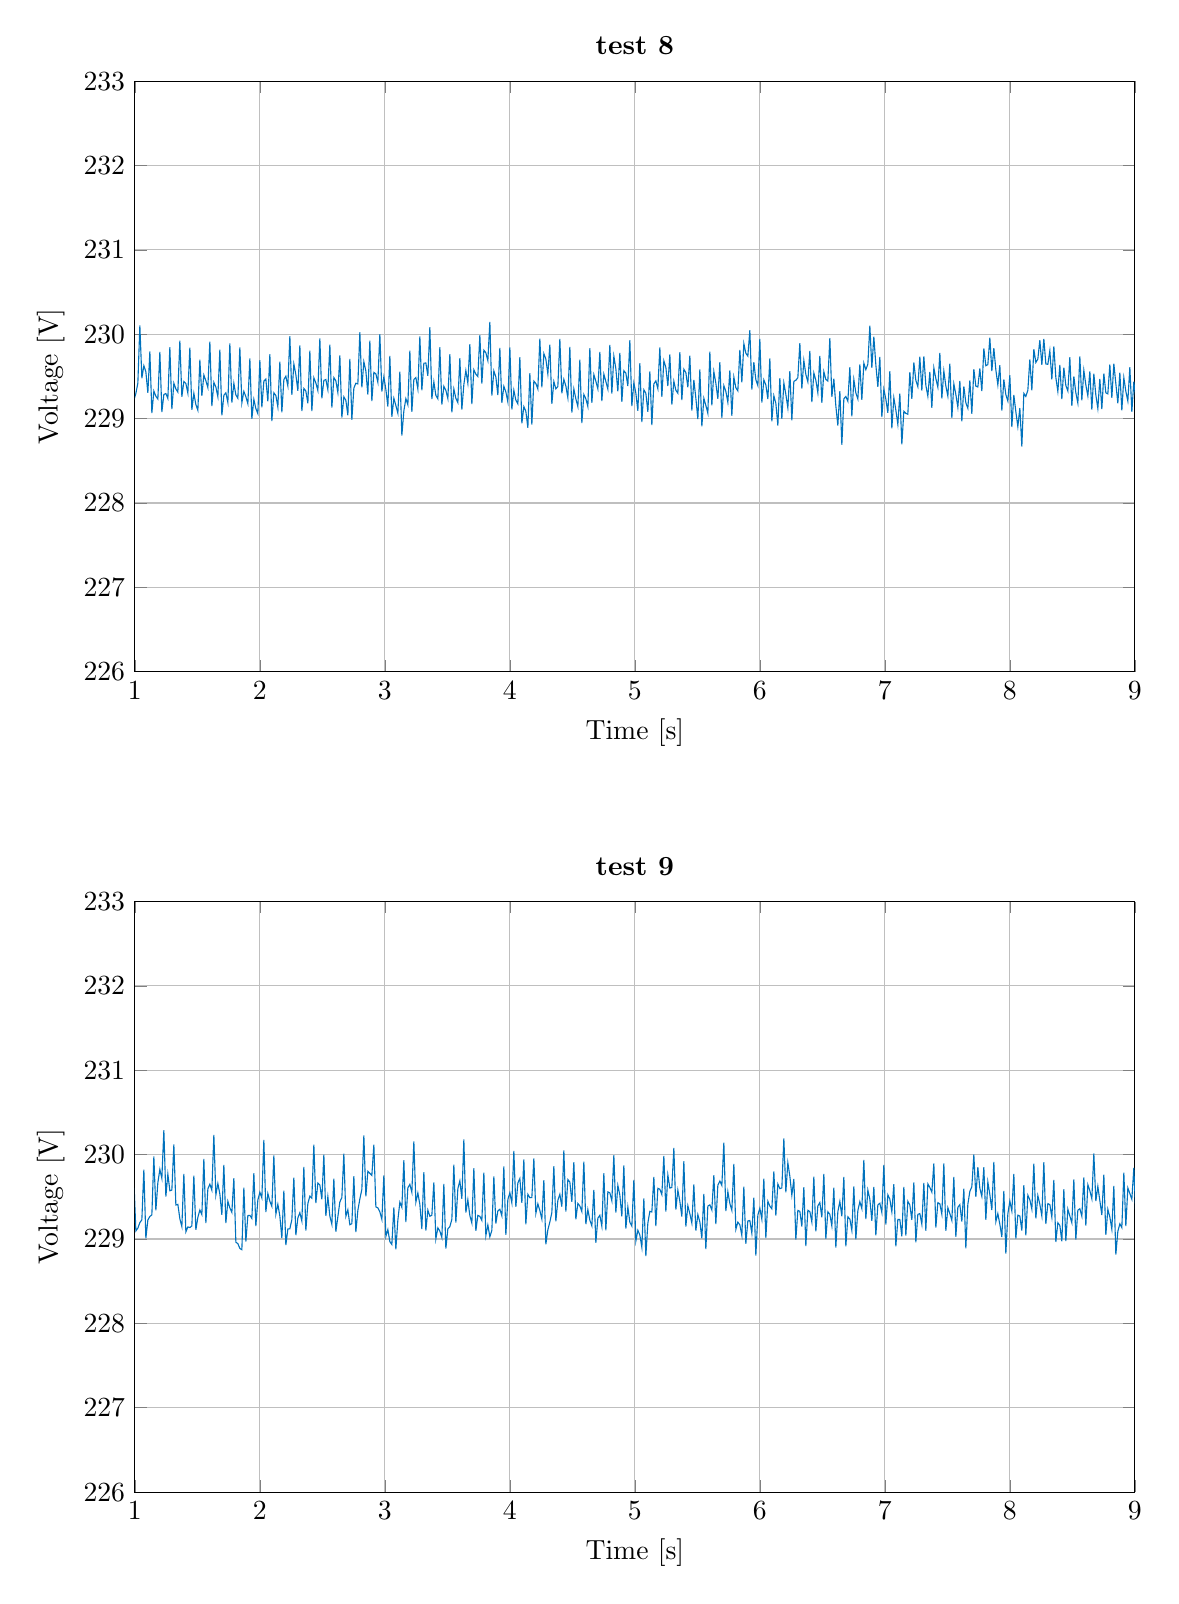
\begin{tikzpicture}

\begin{axis}[%
width=5in,
height=2.953in,
at={(1.142in,5.054in)},
scale only axis,
xmin=1,
xmax=9,
xlabel={Time [s]},
xmajorgrids,
ymin=226,
ymax=233,
ylabel={Voltage [V]},
ymajorgrids,
axis background/.style={fill=white},
title style={font=\bfseries},
title={test 8}
]
\addplot [color=mycolor1,solid,forget plot]
  table[row sep=crcr]{%
0.992	229.215660906661\\
1.008	229.298135833643\\
1.024	229.4197809169\\
1.04	230.104092357186\\
1.056	229.478568649218\\
1.072	229.626366075717\\
1.088	229.555188675072\\
1.104	229.304307937754\\
1.12	229.796268454199\\
1.136	229.06428619795\\
1.152	229.326496594784\\
1.168	229.26484103821\\
1.184	229.231667674679\\
1.2	229.790473072533\\
1.216	229.07788720938\\
1.232	229.286121615709\\
1.248	229.296738048819\\
1.264	229.238628615591\\
1.28	229.847095359705\\
1.296	229.111592249107\\
1.312	229.42007250242\\
1.328	229.351910470775\\
1.344	229.313566543391\\
1.36	229.923125622851\\
1.376	229.259114881277\\
1.392	229.438856306793\\
1.408	229.416015767817\\
1.424	229.302411307644\\
1.44	229.842011365517\\
1.456	229.104413650349\\
1.472	229.299754670142\\
1.488	229.166366004794\\
1.504	229.098751495271\\
1.52	229.697441565087\\
1.536	229.269326464527\\
1.552	229.516365966359\\
1.568	229.448735382719\\
1.584	229.368082443392\\
1.6	229.911869669167\\
1.616	229.146879944844\\
1.632	229.429133576289\\
1.648	229.374372638137\\
1.664	229.260295620547\\
1.68	229.817961372184\\
1.696	229.037519762624\\
1.712	229.276177010435\\
1.728	229.305895328691\\
1.744	229.191752995775\\
1.76	229.890090318109\\
1.776	229.188370977064\\
1.792	229.418356073531\\
1.808	229.280984571422\\
1.824	229.240524941216\\
1.84	229.844348808725\\
1.856	229.186988006938\\
1.872	229.322251369125\\
1.888	229.259745439836\\
1.904	229.177261384152\\
1.92	229.712164555557\\
1.936	228.997691202164\\
1.952	229.227358834196\\
1.968	229.11807531442\\
1.984	229.059572384378\\
2	229.693437722317\\
2.016	229.1339271031\\
2.032	229.443709648304\\
2.048	229.468714533518\\
2.064	229.203630023444\\
2.08	229.762586525112\\
2.096	228.969824989802\\
2.112	229.305476589894\\
2.128	229.273743217598\\
2.144	229.138070735502\\
2.16	229.67421867951\\
2.176	229.074386009092\\
2.192	229.461410140927\\
2.208	229.502460982403\\
2.224	229.387015834455\\
2.24	229.977097258963\\
2.256	229.280125285415\\
2.272	229.647483232962\\
2.288	229.520553728726\\
2.304	229.329649387974\\
2.32	229.867736428206\\
2.336	229.090273758978\\
2.352	229.356760550568\\
2.368	229.326754645978\\
2.384	229.180976743819\\
2.4	229.804584329657\\
2.416	229.088203325551\\
2.432	229.483340855259\\
2.448	229.422115406266\\
2.464	229.332748803986\\
2.48	229.94975774933\\
2.496	229.239291447515\\
2.512	229.452421971485\\
2.528	229.463463003037\\
2.544	229.343779617582\\
2.56	229.87706874785\\
2.576	229.129357249424\\
2.592	229.485826955706\\
2.608	229.447304396066\\
2.624	229.309054480792\\
2.64	229.750382787535\\
2.656	229.011802106961\\
2.672	229.258123351292\\
2.688	229.216631488512\\
2.704	229.039890849123\\
2.72	229.707421308946\\
2.736	228.986192983928\\
2.752	229.36115015887\\
2.768	229.419396859991\\
2.784	229.411006082004\\
2.8	230.023119931966\\
2.816	229.369681827834\\
2.832	229.674013085734\\
2.848	229.564462456677\\
2.864	229.285794962907\\
2.88	229.923992874292\\
2.896	229.207737203383\\
2.912	229.546636062593\\
2.928	229.531091969805\\
2.944	229.430346359641\\
2.96	230.001630072266\\
2.976	229.320417613643\\
2.992	229.494742106281\\
3.008	229.346227829263\\
3.024	229.1435236893\\
3.04	229.743696815765\\
3.056	229.020467259944\\
3.072	229.241136934574\\
3.088	229.155121294884\\
3.104	229.064333392062\\
3.12	229.557200140512\\
3.136	228.798992839063\\
3.152	229.090214613431\\
3.168	229.236815813733\\
3.184	229.164479250309\\
3.2	229.806376471517\\
3.216	229.078642298574\\
3.232	229.463036957679\\
3.248	229.485707357013\\
3.264	229.351013917212\\
3.28	229.974043990031\\
3.296	229.336200224898\\
3.312	229.655733275619\\
3.328	229.659772600434\\
3.344	229.506579944012\\
3.36	230.084639293135\\
3.376	229.230552839906\\
3.392	229.435479615159\\
3.408	229.275643220109\\
3.424	229.23433822935\\
3.44	229.8461519995\\
3.456	229.16640888968\\
3.472	229.383074693003\\
3.488	229.335824207081\\
3.504	229.237282371725\\
3.52	229.764099916261\\
3.536	229.074684655995\\
3.552	229.350543045979\\
3.568	229.240121357751\\
3.584	229.188982925782\\
3.6	229.717444862678\\
3.616	229.106144168299\\
3.632	229.404342383352\\
3.648	229.569118356455\\
3.664	229.41863187076\\
3.68	229.883210027551\\
3.696	229.17118746773\\
3.712	229.578273245292\\
3.728	229.526591325951\\
3.744	229.498541818714\\
3.76	229.989608253154\\
3.776	229.415116016426\\
3.792	229.811072313502\\
3.808	229.78035336516\\
3.824	229.686940162664\\
3.84	230.147012434497\\
3.856	229.272503724728\\
3.872	229.565782355264\\
3.888	229.493931919431\\
3.904	229.277955070592\\
3.92	229.839054375423\\
3.936	229.185490867854\\
3.952	229.382476073471\\
3.968	229.316620667495\\
3.984	229.199344430631\\
4	229.845089626701\\
4.016	229.108154544852\\
4.032	229.337306316279\\
4.048	229.21909981101\\
4.064	229.175028145282\\
4.08	229.72765916127\\
4.096	228.94346715271\\
4.112	229.141698252073\\
4.128	229.086592205384\\
4.144	228.891096702992\\
4.16	229.539589773474\\
4.176	228.927567107321\\
4.192	229.444459351568\\
4.208	229.415874355435\\
4.224	229.350912764681\\
4.24	229.947605465271\\
4.256	229.371683891881\\
4.272	229.770080459263\\
4.288	229.705471128722\\
4.304	229.529514791928\\
4.32	229.876134005518\\
4.336	229.174397015554\\
4.352	229.439492343087\\
4.368	229.352709776683\\
4.384	229.379969107527\\
4.4	229.943145384196\\
4.416	229.299381150698\\
4.432	229.464603295204\\
4.448	229.386389081574\\
4.464	229.247657679501\\
4.48	229.849159103118\\
4.496	229.071281893723\\
4.512	229.351208616023\\
4.528	229.234377021463\\
4.544	229.143666117659\\
4.56	229.697238205908\\
4.576	228.947402732576\\
4.592	229.285855438678\\
4.608	229.234778464806\\
4.624	229.143293474419\\
4.64	229.835840746861\\
4.656	229.186683241919\\
4.672	229.521609009181\\
4.688	229.442610644395\\
4.704	229.352689572463\\
4.72	229.79118712959\\
4.736	229.208012769987\\
4.752	229.527315749968\\
4.768	229.439730276759\\
4.784	229.350721563552\\
4.8	229.87386275335\\
4.816	229.297094961862\\
4.832	229.740189034963\\
4.848	229.591404442217\\
4.864	229.32221974023\\
4.88	229.77987520829\\
4.896	229.197265144314\\
4.912	229.567711118273\\
4.928	229.539019112472\\
4.944	229.385152787029\\
4.96	229.928765439307\\
4.976	229.147902073855\\
4.992	229.423365306433\\
5.008	229.301524502981\\
5.024	229.0912153979\\
5.04	229.656625169261\\
5.056	228.959832173375\\
5.072	229.341384231898\\
5.088	229.300098583624\\
5.104	229.080473717489\\
5.12	229.560624461295\\
5.136	228.922175675451\\
5.152	229.411539138412\\
5.168	229.446923385499\\
5.184	229.354972880064\\
5.2	229.842770908417\\
5.216	229.256561896778\\
5.232	229.684754975306\\
5.248	229.607353725382\\
5.264	229.386819909145\\
5.28	229.760391307605\\
5.296	229.165905668138\\
5.312	229.442399493084\\
5.328	229.335719540336\\
5.344	229.300470449942\\
5.36	229.786375650945\\
5.376	229.219661154471\\
5.392	229.584776492977\\
5.408	229.545116706476\\
5.424	229.371665293611\\
5.44	229.745616738851\\
5.456	229.096096702613\\
5.472	229.458841669808\\
5.488	229.243268805715\\
5.504	228.993927295684\\
5.52	229.582970303046\\
5.536	228.908602412743\\
5.552	229.239852084743\\
5.568	229.155896856753\\
5.584	229.062693287762\\
5.6	229.794197694347\\
5.616	229.156931530704\\
5.632	229.557123404506\\
5.648	229.419134828248\\
5.664	229.234734510544\\
5.68	229.668502486651\\
5.696	229.009267764456\\
5.712	229.390051734771\\
5.728	229.322540374843\\
5.744	229.192626701306\\
5.76	229.570614778756\\
5.776	229.033669134698\\
5.792	229.492153053831\\
5.808	229.365689612917\\
5.824	229.328715917087\\
5.84	229.814418271884\\
5.856	229.428743437498\\
5.872	229.889051932059\\
5.888	229.774677063228\\
5.904	229.740741964928\\
5.92	230.047294801451\\
5.936	229.342619051404\\
5.952	229.667632936269\\
5.968	229.459548337818\\
5.984	229.392508465476\\
6	229.94526748273\\
6.016	229.190347117459\\
6.032	229.458535575629\\
6.048	229.399532121354\\
6.064	229.232067747244\\
6.08	229.713029649796\\
6.096	228.966892600863\\
6.112	229.270592925351\\
6.128	229.180626589129\\
6.144	228.917674742062\\
6.16	229.480153017486\\
6.176	228.996271035131\\
6.192	229.422924539713\\
6.208	229.286280050125\\
6.224	229.127397307656\\
6.24	229.563171412504\\
6.256	228.97883786168\\
6.272	229.441208327697\\
6.288	229.454032066099\\
6.304	229.485534547499\\
6.32	229.895543572315\\
6.336	229.354954113106\\
6.352	229.688996773316\\
6.368	229.52221438675\\
6.384	229.436114856138\\
6.4	229.801375797199\\
6.416	229.194378707467\\
6.432	229.540761683888\\
6.448	229.454640135741\\
6.464	229.306593072637\\
6.48	229.743678145171\\
6.496	229.187359617138\\
6.512	229.555473192726\\
6.528	229.464037744485\\
6.544	229.445120582738\\
6.56	229.952918653365\\
6.576	229.257182711305\\
6.592	229.473174129013\\
6.608	229.150610558354\\
6.624	228.916583934022\\
6.64	229.32623410883\\
6.656	228.689681763651\\
6.672	229.234960008348\\
6.688	229.261846230261\\
6.704	229.205903684475\\
6.72	229.60867777027\\
6.736	229.027526881539\\
6.752	229.463283446909\\
6.768	229.304933448574\\
6.784	229.232902375633\\
6.8	229.641221453795\\
6.816	229.222044042396\\
6.832	229.657516374666\\
6.848	229.580201443819\\
6.864	229.644933041904\\
6.88	230.10120100302\\
6.896	229.602165714518\\
6.912	229.970825992309\\
6.928	229.636856550933\\
6.944	229.375313675663\\
6.96	229.729793251697\\
6.976	229.018243826426\\
6.992	229.347957829565\\
7.008	229.23137167407\\
7.024	229.067581451552\\
7.04	229.563535397593\\
7.056	228.883194630574\\
7.072	229.246709653438\\
7.088	229.101717416914\\
7.104	228.931308626287\\
7.12	229.296991250605\\
7.136	228.695444224666\\
7.152	229.086325707182\\
7.168	229.062099001779\\
7.184	229.051588430937\\
7.2	229.551365151024\\
7.216	229.232967665545\\
7.232	229.664847182513\\
7.248	229.452791819712\\
7.264	229.379000198049\\
7.28	229.732783821998\\
7.296	229.331990349059\\
7.312	229.73842808398\\
7.328	229.394485205905\\
7.344	229.265990614332\\
7.36	229.55440539639\\
7.376	229.127366610731\\
7.392	229.601315962859\\
7.408	229.474388516231\\
7.424	229.372091451947\\
7.44	229.777882035668\\
7.456	229.238480159337\\
7.472	229.564302383041\\
7.488	229.38640112434\\
7.504	229.266887732554\\
7.52	229.650705981375\\
7.536	229.007936152844\\
7.552	229.41166197508\\
7.568	229.285704140466\\
7.584	229.134573411268\\
7.6	229.447947284895\\
7.616	228.967851465346\\
7.632	229.38190952986\\
7.648	229.187226666622\\
7.664	229.122235576255\\
7.68	229.451203153207\\
7.696	229.056869488589\\
7.712	229.585192688382\\
7.728	229.383644023313\\
7.744	229.374775413933\\
7.76	229.593521223451\\
7.776	229.324735051008\\
7.792	229.830602600388\\
7.808	229.626765505407\\
7.824	229.640006240118\\
7.84	229.95849188002\\
7.856	229.564113216433\\
7.872	229.835141447604\\
7.888	229.577689709799\\
7.904	229.400018182566\\
7.92	229.633855481169\\
7.936	229.095911014751\\
7.952	229.464032133166\\
7.968	229.283114917035\\
7.984	229.208040522275\\
8	229.513744834145\\
8.016	228.900656563765\\
8.032	229.279624145659\\
8.048	229.081441387915\\
8.064	228.904879920009\\
8.08	229.124942195694\\
8.096	228.669087387695\\
8.112	229.298905706788\\
8.128	229.262748089459\\
8.144	229.333917841673\\
8.16	229.702259190522\\
8.176	229.33390587737\\
8.192	229.821824545826\\
8.208	229.664993874368\\
8.224	229.706312610552\\
8.24	229.930224078385\\
8.256	229.636677926694\\
8.272	229.944945328503\\
8.288	229.647435230488\\
8.304	229.642911955852\\
8.32	229.804934522768\\
8.336	229.463741837706\\
8.352	229.854596940071\\
8.368	229.485971639765\\
8.384	229.323062944073\\
8.4	229.63508886211\\
8.416	229.229892158922\\
8.432	229.604185113324\\
8.448	229.392263022183\\
8.464	229.327400981701\\
8.48	229.728193747875\\
8.496	229.149698598966\\
8.512	229.49968498515\\
8.528	229.30571750782\\
8.544	229.184181435447\\
8.56	229.736610963314\\
8.576	229.215530733814\\
8.592	229.572150603428\\
8.608	229.398504661232\\
8.624	229.268854718724\\
8.64	229.560367691362\\
8.656	229.105493701278\\
8.672	229.5317557452\\
8.688	229.27914938689\\
8.704	229.120129391208\\
8.72	229.47134056995\\
8.736	229.111576911684\\
8.752	229.533916321481\\
8.768	229.305713186958\\
8.784	229.292747150921\\
8.8	229.64067665739\\
8.816	229.245573444196\\
8.832	229.651073276237\\
8.848	229.413934473195\\
8.864	229.182271094187\\
8.88	229.545190997241\\
8.896	229.097129337999\\
8.912	229.484743032199\\
8.928	229.323106704037\\
8.944	229.206918033804\\
8.96	229.608650028152\\
8.976	229.080863365453\\
8.992	229.438996476506\\
9.008	229.232692707784\\
};
\end{axis}

\begin{axis}[%
width=5in,
height=2.953in,
at={(1.142in,0.952in)},
scale only axis,
xmin=1,
xmax=9,
xlabel={Time [s]},
xmajorgrids,
ymin=226,
ymax=233,
ylabel={Voltage [V]},
ymajorgrids,
axis background/.style={fill=white},
title style={font=\bfseries},
title={test 9}
]
\addplot [color=mycolor1,solid,forget plot]
  table[row sep=crcr]{%
0.992	229.709230529955\\
1.008	229.095386595861\\
1.024	229.128664291696\\
1.04	229.194738721229\\
1.056	229.226969988416\\
1.072	229.82173820616\\
1.088	229.007321043809\\
1.104	229.225610691539\\
1.12	229.266544556989\\
1.136	229.285739802093\\
1.152	229.97774482898\\
1.168	229.338684468429\\
1.184	229.667285629675\\
1.2	229.825015618384\\
1.216	229.718858164762\\
1.232	230.289834233912\\
1.248	229.5026033771\\
1.264	229.768762275799\\
1.28	229.571538120713\\
1.296	229.580230062021\\
1.312	230.120217634541\\
1.328	229.402705405492\\
1.344	229.410210923241\\
1.36	229.239476779794\\
1.376	229.14651224585\\
1.392	229.771195174039\\
1.408	229.084320130011\\
1.424	229.142645902931\\
1.44	229.135409790818\\
1.456	229.155203688454\\
1.472	229.751533773437\\
1.488	229.107675745976\\
1.504	229.257107846016\\
1.52	229.343063183\\
1.536	229.289133306345\\
1.552	229.949192799053\\
1.568	229.188954384866\\
1.584	229.59442549165\\
1.6	229.649201775786\\
1.616	229.578687177851\\
1.632	230.235092998581\\
1.648	229.521946068067\\
1.664	229.657502051324\\
1.68	229.533159725427\\
1.696	229.285715918066\\
1.712	229.878921796005\\
1.728	229.189777974735\\
1.744	229.447179937766\\
1.76	229.367877001006\\
1.776	229.316116988304\\
1.792	229.72110406501\\
1.808	228.96097721234\\
1.824	228.944801064917\\
1.84	228.888191623918\\
1.856	228.872666151625\\
1.872	229.609697230109\\
1.888	228.968625862161\\
1.904	229.277879083154\\
1.92	229.280225299137\\
1.936	229.24372960208\\
1.952	229.780667185358\\
1.968	229.1530841168\\
1.984	229.462200365539\\
2	229.553772698895\\
2.016	229.48639814871\\
2.032	230.173166578471\\
2.048	229.320076428408\\
2.064	229.53944913047\\
2.08	229.44584690942\\
2.096	229.387115750447\\
2.112	229.990407764616\\
2.128	229.2944562751\\
2.144	229.411454632197\\
2.16	229.270606542881\\
2.176	229.010684256592\\
2.192	229.572203344093\\
2.208	228.928000406375\\
2.224	229.118927197495\\
2.24	229.121397822804\\
2.256	229.230353165601\\
2.272	229.728049673971\\
2.288	229.045013150641\\
2.304	229.250151142926\\
2.32	229.311954727022\\
2.336	229.213030339231\\
2.352	229.853695513927\\
2.368	229.099967455563\\
2.384	229.42032019125\\
2.4	229.507994643729\\
2.416	229.483824955401\\
2.432	230.118627433131\\
2.448	229.425205130078\\
2.464	229.663584694897\\
2.48	229.639668910086\\
2.496	229.470831209482\\
2.512	229.999587253086\\
2.528	229.2730566746\\
2.544	229.501799974819\\
2.56	229.270807077554\\
2.576	229.174004250721\\
2.592	229.716698053998\\
2.608	229.086381121962\\
2.624	229.262191379064\\
2.64	229.440418606563\\
2.656	229.490042145462\\
2.672	230.010253736201\\
2.688	229.268255925007\\
2.704	229.346186206638\\
2.72	229.168672845402\\
2.736	229.181962940345\\
2.752	229.744545943722\\
2.768	229.081559529125\\
2.784	229.339087803098\\
2.8	229.474527857861\\
2.816	229.588354853297\\
2.832	230.227926059187\\
2.848	229.505223842673\\
2.864	229.80228069406\\
2.88	229.777605574806\\
2.896	229.754132176001\\
2.912	230.117578779836\\
2.928	229.380875733502\\
2.944	229.369476268776\\
2.96	229.321388893981\\
2.976	229.233066846901\\
2.992	229.752478182035\\
3.008	229.030597958842\\
3.024	229.111065129794\\
3.04	228.968428960159\\
3.056	228.934706632147\\
3.072	229.373082770276\\
3.088	228.878028033086\\
3.104	229.223624695272\\
3.12	229.436372239644\\
3.136	229.375674866826\\
3.152	229.933306158894\\
3.168	229.201316988272\\
3.184	229.606234632071\\
3.2	229.647084261261\\
3.216	229.55294877397\\
3.232	230.15609767077\\
3.248	229.436246777301\\
3.264	229.544765985019\\
3.28	229.410632401919\\
3.296	229.118422008358\\
3.312	229.793412628375\\
3.328	229.099692934326\\
3.344	229.342738280646\\
3.36	229.269183831102\\
3.376	229.280898015\\
3.392	229.6705570656\\
3.408	229.001346452062\\
3.424	229.132387533013\\
3.44	229.092873276991\\
3.456	229.016778932997\\
3.472	229.652027126822\\
3.488	228.886141440448\\
3.504	229.12090614785\\
3.52	229.14630774\\
3.536	229.232872177457\\
3.552	229.879841197349\\
3.568	229.195180184908\\
3.584	229.596894805972\\
3.6	229.689202172334\\
3.616	229.475298577348\\
3.632	230.179395754065\\
3.648	229.314147222109\\
3.664	229.465671896654\\
3.68	229.276907948496\\
3.696	229.189364192946\\
3.712	229.839341294692\\
3.728	229.095826206931\\
3.744	229.280026361864\\
3.76	229.267773583028\\
3.776	229.220391176538\\
3.792	229.786210329418\\
3.808	229.039578489506\\
3.824	229.165725863623\\
3.84	229.025821378489\\
3.856	229.101918222812\\
3.872	229.742268877516\\
3.888	229.182182122399\\
3.904	229.332963901462\\
3.92	229.352661940505\\
3.936	229.275027213619\\
3.952	229.859211655531\\
3.968	229.048968012193\\
3.984	229.467255954513\\
4	229.548828245736\\
4.016	229.427869597797\\
4.032	230.043894282672\\
4.048	229.379926336508\\
4.064	229.664018101633\\
4.08	229.716742139649\\
4.096	229.429198291706\\
4.112	229.942910681018\\
4.128	229.174792968892\\
4.144	229.529698784739\\
4.16	229.489275042215\\
4.176	229.490717025386\\
4.192	229.954373452355\\
4.208	229.303157044517\\
4.224	229.41668223749\\
4.24	229.336721928751\\
4.256	229.236025155343\\
4.272	229.69845873281\\
4.288	228.936858830511\\
4.304	229.108615247753\\
4.32	229.201245862795\\
4.336	229.313942277794\\
4.352	229.862197848025\\
4.368	229.210288768319\\
4.384	229.457277343453\\
4.4	229.528625556312\\
4.416	229.382971887932\\
4.432	230.049299517338\\
4.448	229.325192803962\\
4.464	229.704568677103\\
4.48	229.674497301471\\
4.496	229.440112874421\\
4.512	229.911207483356\\
4.528	229.233397433789\\
4.544	229.420796782318\\
4.56	229.391226442888\\
4.576	229.324716866583\\
4.592	229.915586556962\\
4.608	229.175408697283\\
4.624	229.349150474859\\
4.64	229.223341748861\\
4.656	229.155596003651\\
4.672	229.582719163762\\
4.688	228.955669443074\\
4.704	229.246825770548\\
4.72	229.280758468988\\
4.736	229.151020057934\\
4.752	229.779425229834\\
4.768	229.10189825011\\
4.784	229.557980240863\\
4.8	229.546428928819\\
4.816	229.452316051418\\
4.832	229.994078584558\\
4.848	229.312911483922\\
4.864	229.635462298019\\
4.88	229.519901222646\\
4.896	229.26714025524\\
4.912	229.873648848811\\
4.928	229.122890424137\\
4.944	229.379429560076\\
4.96	229.198665134918\\
4.976	229.15180233352\\
4.992	229.699228867834\\
5.008	228.975627134023\\
5.024	229.103241272656\\
5.04	229.047010946743\\
5.056	228.900197672769\\
5.072	229.480841152883\\
5.088	228.797639652983\\
5.104	229.188218609593\\
5.12	229.327868781027\\
5.136	229.320459439217\\
5.152	229.735789916939\\
5.168	229.153679165599\\
5.184	229.60073164236\\
5.2	229.589897506828\\
5.216	229.526685296762\\
5.232	229.985721055538\\
5.248	229.325829843748\\
5.264	229.759327218759\\
5.28	229.603680132237\\
5.296	229.610622104137\\
5.312	230.07873667003\\
5.328	229.347396329758\\
5.344	229.580057718498\\
5.36	229.445891249936\\
5.376	229.264608166913\\
5.392	229.922748943384\\
5.408	229.148008233164\\
5.424	229.394639420002\\
5.44	229.299306651336\\
5.456	229.187979220457\\
5.472	229.645599941517\\
5.488	229.098373056648\\
5.504	229.28936574442\\
5.52	229.202381052902\\
5.536	229.007115706648\\
5.552	229.535476269454\\
5.568	228.878999803624\\
5.584	229.389959583691\\
5.6	229.404687915076\\
5.616	229.343979957218\\
5.632	229.756421069861\\
5.648	229.176897807742\\
5.664	229.638125304905\\
5.68	229.686831468778\\
5.696	229.635219439687\\
5.712	230.143363514056\\
5.728	229.330437563922\\
5.744	229.561028984366\\
5.76	229.421139245684\\
5.776	229.339613035\\
5.792	229.89014929693\\
5.808	229.114076104056\\
5.824	229.199912056895\\
5.84	229.167400902448\\
5.856	229.041306459654\\
5.872	229.619853595464\\
5.888	228.943839452822\\
5.904	229.214060248234\\
5.92	229.218740897153\\
5.936	229.066864665776\\
5.952	229.490343524624\\
5.968	228.802762246012\\
5.984	229.283866331789\\
6	229.364777604654\\
6.016	229.233169623681\\
6.032	229.716620837351\\
6.048	229.010010333102\\
6.064	229.447257029031\\
6.08	229.388750344659\\
6.096	229.357677088656\\
6.112	229.800422041788\\
6.128	229.27630723945\\
6.144	229.652002589315\\
6.16	229.596613897069\\
6.176	229.605507778346\\
6.192	230.192526453627\\
6.208	229.55389471089\\
6.224	229.904553834386\\
6.24	229.743547565027\\
6.256	229.519240137377\\
6.272	229.711158718312\\
6.288	228.993526327907\\
6.304	229.338633783403\\
6.32	229.328262260655\\
6.336	229.147959000495\\
6.352	229.614033555627\\
6.368	228.916424384955\\
6.384	229.339967240323\\
6.4	229.325056888435\\
6.416	229.201417735011\\
6.432	229.737847460128\\
6.448	229.09045237122\\
6.464	229.39265031555\\
6.48	229.432488830235\\
6.496	229.255771164521\\
6.512	229.772155740238\\
6.528	229.002179076344\\
6.544	229.3225616382\\
6.56	229.292939712764\\
6.576	229.154165570786\\
6.592	229.608288419612\\
6.608	228.897365862441\\
6.624	229.323662028906\\
6.64	229.445506103442\\
6.656	229.268846195169\\
6.672	229.735362317533\\
6.688	228.912993753206\\
6.704	229.262616378041\\
6.72	229.23696399848\\
6.736	229.101439299739\\
6.752	229.62309873821\\
6.768	228.996758293557\\
6.784	229.335575902928\\
6.8	229.442590905569\\
6.816	229.360282840826\\
6.832	229.936226959773\\
6.848	229.236980401762\\
6.864	229.579736650536\\
6.88	229.472100804687\\
6.896	229.215529196494\\
6.912	229.616920149088\\
6.928	229.042629579507\\
6.944	229.403346173505\\
6.96	229.424017666741\\
6.976	229.314452914219\\
6.992	229.878456583746\\
7.008	229.17101937179\\
7.024	229.523346587278\\
7.04	229.471675414352\\
7.056	229.321327859444\\
7.072	229.650954789074\\
7.088	228.912661674543\\
7.104	229.231111003506\\
7.12	229.230460650102\\
7.136	229.03022698944\\
7.152	229.617819903369\\
7.168	229.041608071368\\
7.184	229.447982921511\\
7.2	229.400826682106\\
7.216	229.225845690093\\
7.232	229.669917029572\\
7.248	228.961490722371\\
7.264	229.292398915457\\
7.28	229.30082232395\\
7.296	229.174363279106\\
7.312	229.663854952696\\
7.328	229.097824878982\\
7.344	229.653237073424\\
7.36	229.611264620198\\
7.376	229.555402340703\\
7.392	229.894775708375\\
7.408	229.135340651683\\
7.424	229.430742157995\\
7.44	229.417707413131\\
7.456	229.292656232811\\
7.472	229.895307074297\\
7.488	229.097541414824\\
7.504	229.370158138126\\
7.52	229.301310383451\\
7.536	229.220789994256\\
7.552	229.736059045238\\
7.568	229.026421719647\\
7.584	229.375720280206\\
7.6	229.407341859293\\
7.616	229.206669686684\\
7.632	229.596677501876\\
7.648	228.889633021551\\
7.664	229.412020944449\\
7.68	229.56425827944\\
7.696	229.619813919014\\
7.712	230.00110041117\\
7.728	229.498352979134\\
7.744	229.850703637201\\
7.76	229.600597940845\\
7.776	229.504323418684\\
7.792	229.85033524334\\
7.808	229.226970698147\\
7.824	229.67710327758\\
7.84	229.526033193605\\
7.856	229.342474030669\\
7.872	229.913044657399\\
7.888	229.206155325586\\
7.904	229.300704749351\\
7.92	229.174270270834\\
7.936	229.022741865461\\
7.952	229.571208217445\\
7.968	228.825811017672\\
7.984	229.296891604127\\
8	229.449825267098\\
8.016	229.330176349086\\
8.032	229.771425004591\\
8.048	229.00404241811\\
8.064	229.282508178542\\
8.08	229.27250548489\\
8.096	229.098615545896\\
8.112	229.637336262308\\
8.128	229.042601562074\\
8.144	229.519453567825\\
8.16	229.464514575683\\
8.176	229.353729934824\\
8.192	229.892400306979\\
8.208	229.243404448798\\
8.224	229.514632741799\\
8.24	229.41041817609\\
8.256	229.272413935675\\
8.272	229.90944865509\\
8.288	229.178107486805\\
8.304	229.419189301914\\
8.32	229.408368155485\\
8.336	229.257249869785\\
8.352	229.699095041128\\
8.368	228.964839270782\\
8.384	229.19245092864\\
8.4	229.160641136688\\
8.416	228.973101803223\\
8.432	229.590880034825\\
8.448	228.9737675136\\
8.464	229.353906510238\\
8.48	229.272540732312\\
8.496	229.192311749498\\
8.512	229.706591167067\\
8.528	228.993630956715\\
8.544	229.340838704043\\
8.56	229.359003808132\\
8.576	229.269638941748\\
8.592	229.729268368444\\
8.608	229.157669548105\\
8.624	229.644524140564\\
8.64	229.572046450287\\
8.656	229.476477134789\\
8.672	230.013121937169\\
8.688	229.448486662502\\
8.704	229.623971806806\\
8.72	229.453660592164\\
8.736	229.283206544393\\
8.752	229.76301860223\\
8.768	229.048781365296\\
8.784	229.352104515582\\
8.8	229.259486808496\\
8.816	229.115464566589\\
8.832	229.629621051688\\
8.848	228.8157108935\\
8.864	229.090789840172\\
8.88	229.17934832248\\
8.896	229.134757232942\\
8.912	229.784899352316\\
8.928	229.153166281658\\
8.944	229.605324202946\\
8.96	229.53895125069\\
8.976	229.470717056439\\
8.992	229.843992220291\\
9.008	229.266501980315\\
};
\end{axis}
\end{tikzpicture}%
\caption{Steady state Voltage output of the genset at 10 kW load.}
\label{fig:test8-9steadyvolt10kw}
\end{figure}

\begin{figure}[H]
\centering
% This file was created by matlab2tikz.
%
%The latest updates can be retrieved from
%  http://www.mathworks.com/matlabcentral/fileexchange/22022-matlab2tikz-matlab2tikz
%where you can also make suggestions and rate matlab2tikz.
%
\definecolor{mycolor1}{rgb}{0.00000,0.44700,0.74100}%
%
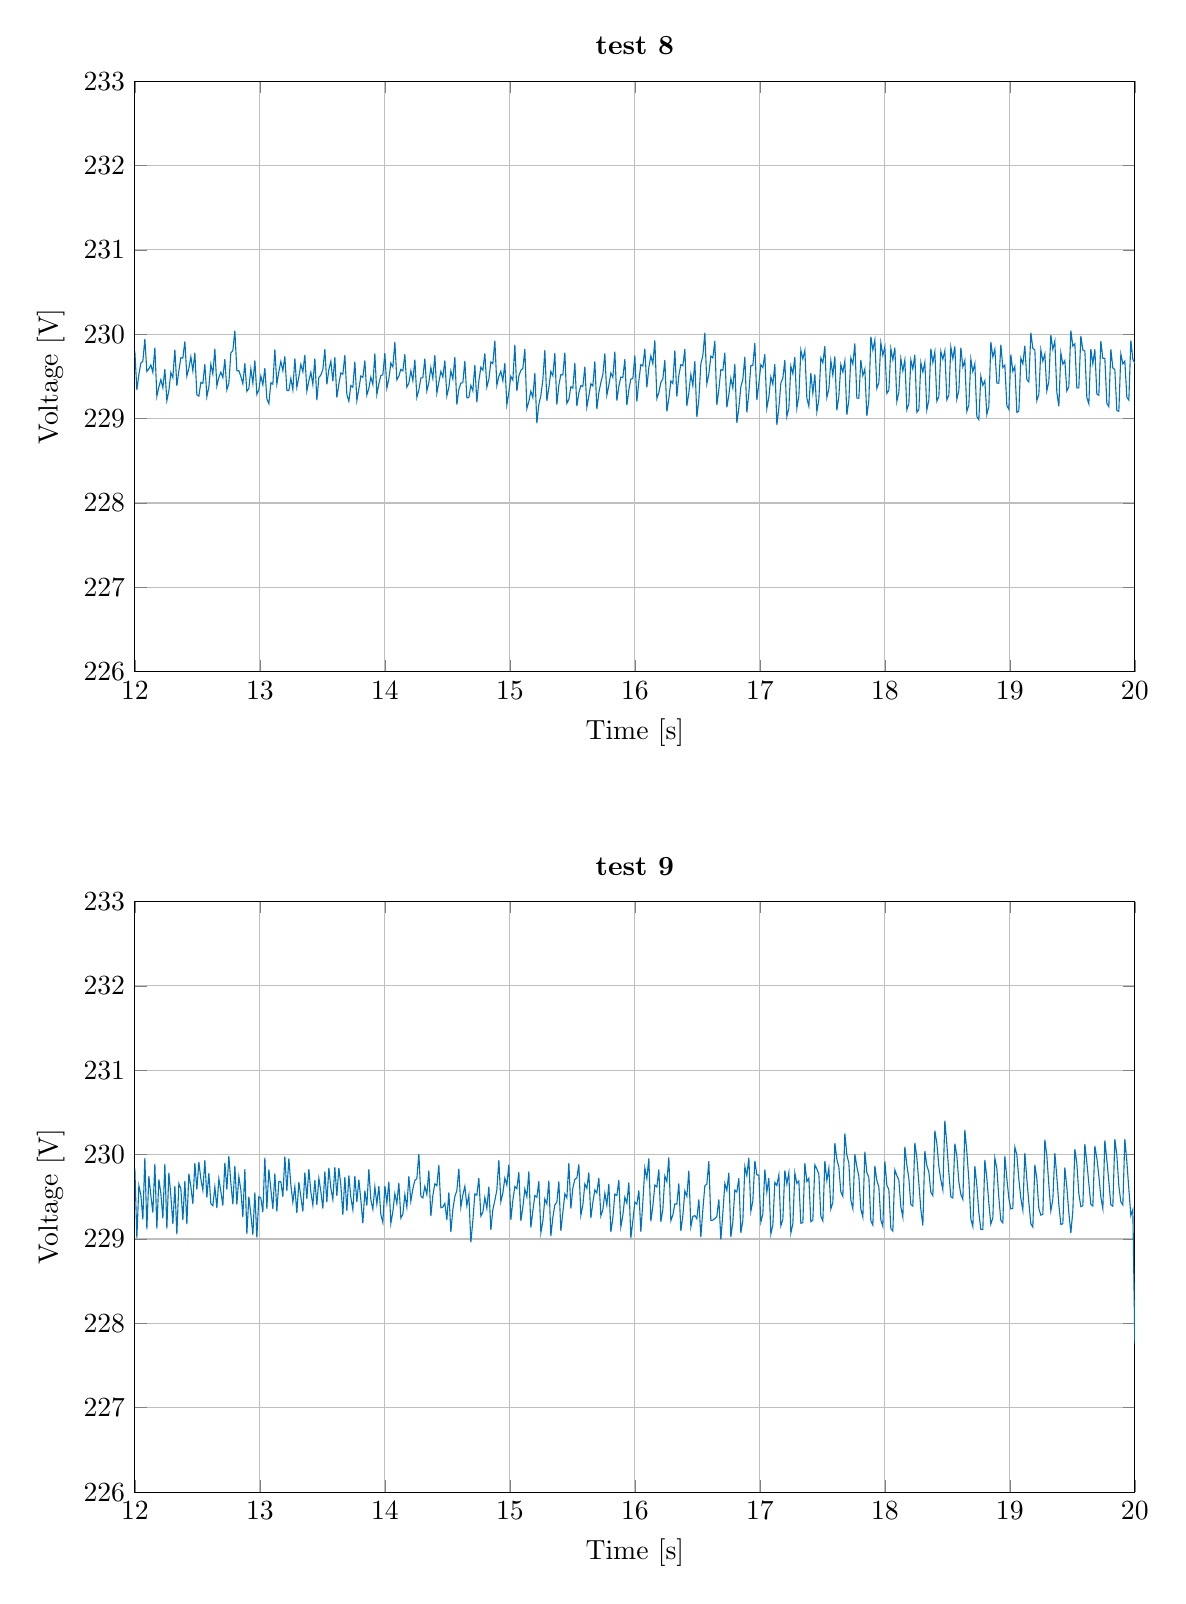
\begin{tikzpicture}

\begin{axis}[%
width=5in,
height=2.953in,
at={(1.142in,5.054in)},
scale only axis,
xmin=12,
xmax=20,
xlabel={Time [s]},
xmajorgrids,
ymin=226,
ymax=233,
ylabel={Voltage [V]},
ymajorgrids,
axis background/.style={fill=white},
title style={font=\bfseries},
title={test 8}
]
\addplot [color=mycolor1,solid,forget plot]
  table[row sep=crcr]{%
12	229.795501798809\\
12.016	229.338918767167\\
12.032	229.522175622486\\
12.048	229.657943170422\\
12.064	229.679382936229\\
12.08	229.943205077002\\
12.096	229.559027126838\\
12.112	229.589907613865\\
12.128	229.635281790919\\
12.144	229.547549234745\\
12.16	229.841144516788\\
12.176	229.26410711835\\
12.192	229.373279077127\\
12.208	229.462163285366\\
12.224	229.365530558835\\
12.24	229.587397029621\\
12.256	229.21256003735\\
12.272	229.328949592192\\
12.288	229.546184469914\\
12.304	229.484713177742\\
12.32	229.81739438526\\
12.336	229.388660010418\\
12.352	229.565362074789\\
12.368	229.721229447935\\
12.384	229.717749408731\\
12.4	229.914681683179\\
12.416	229.503632974924\\
12.432	229.594635097423\\
12.448	229.733155829848\\
12.464	229.565457776844\\
12.48	229.780237683196\\
12.496	229.281558857126\\
12.512	229.266574421158\\
12.528	229.428625907684\\
12.544	229.417366369585\\
12.56	229.645296389353\\
12.576	229.259356906071\\
12.592	229.374042277722\\
12.608	229.644855405841\\
12.624	229.528479157966\\
12.64	229.827520969543\\
12.656	229.38605488548\\
12.672	229.488379505456\\
12.688	229.550806371644\\
12.704	229.485290782731\\
12.72	229.703229722902\\
12.736	229.341520895567\\
12.752	229.419572997273\\
12.768	229.77922017273\\
12.784	229.806649988293\\
12.8	230.04172866853\\
12.816	229.566569373997\\
12.832	229.567797985895\\
12.848	229.498948495748\\
12.864	229.412736601276\\
12.88	229.655872020853\\
12.896	229.323234632462\\
12.912	229.356024442031\\
12.928	229.588794185134\\
12.944	229.418525179485\\
12.96	229.688609997748\\
12.976	229.286553835239\\
12.992	229.342457000299\\
13.008	229.504339406468\\
13.024	229.399862346196\\
13.04	229.59803677247\\
13.056	229.2340810874\\
13.072	229.176965664918\\
13.088	229.424194323219\\
13.104	229.407892570879\\
13.12	229.819331186574\\
13.136	229.409399720435\\
13.152	229.554398503198\\
13.168	229.677041593998\\
13.184	229.567572203653\\
13.2	229.738200806105\\
13.216	229.33390756904\\
13.232	229.332200613581\\
13.248	229.47623823984\\
13.264	229.341547434551\\
13.28	229.713018871674\\
13.296	229.369597028075\\
13.312	229.494679977371\\
13.328	229.643951658667\\
13.344	229.553707175047\\
13.36	229.754468920664\\
13.376	229.32566618179\\
13.392	229.447109261994\\
13.408	229.550128371837\\
13.424	229.403814636556\\
13.44	229.714113230977\\
13.456	229.217872384689\\
13.472	229.488518162302\\
13.488	229.515602320612\\
13.504	229.581773705065\\
13.52	229.822447442449\\
13.536	229.405488901679\\
13.552	229.581002816517\\
13.568	229.679910922131\\
13.584	229.442050160906\\
13.6	229.72868148717\\
13.616	229.248337156256\\
13.632	229.40981248917\\
13.648	229.541634689195\\
13.664	229.525028447761\\
13.68	229.753005038916\\
13.696	229.285795274663\\
13.712	229.205639701436\\
13.728	229.392727707142\\
13.744	229.370748351914\\
13.76	229.675706144266\\
13.776	229.213019937314\\
13.792	229.350446549647\\
13.808	229.505814420353\\
13.824	229.488066611932\\
13.84	229.688468250866\\
13.856	229.278916482042\\
13.872	229.35890900276\\
13.888	229.491927588225\\
13.904	229.403175924969\\
13.92	229.772185984114\\
13.936	229.284920742371\\
13.952	229.414166410609\\
13.968	229.511170121651\\
13.984	229.51856825301\\
14	229.775788442974\\
14.016	229.360360930855\\
14.032	229.470606319556\\
14.048	229.658044372697\\
14.064	229.611894241221\\
14.08	229.907739085564\\
14.096	229.45952135007\\
14.112	229.503591453493\\
14.128	229.583817781762\\
14.144	229.565090426878\\
14.16	229.762009012863\\
14.176	229.372349419061\\
14.192	229.420333100438\\
14.208	229.566736163267\\
14.224	229.449647518623\\
14.24	229.699506071768\\
14.256	229.250260981703\\
14.272	229.339248063721\\
14.288	229.480620636834\\
14.304	229.485229866626\\
14.32	229.711546217971\\
14.336	229.32705434973\\
14.352	229.425986552671\\
14.368	229.6042982859\\
14.384	229.476345236679\\
14.4	229.751775212175\\
14.416	229.30137169114\\
14.432	229.430418052354\\
14.448	229.559216475421\\
14.464	229.493258224456\\
14.48	229.688639935051\\
14.496	229.268514433968\\
14.512	229.36955776355\\
14.528	229.565036674425\\
14.544	229.46824623405\\
14.56	229.731005526493\\
14.576	229.166523580414\\
14.592	229.345091799542\\
14.608	229.420498197953\\
14.624	229.425532350674\\
14.64	229.68239422444\\
14.656	229.24635438798\\
14.672	229.248315642051\\
14.688	229.393583967491\\
14.704	229.329546723581\\
14.72	229.636696283645\\
14.736	229.194015315582\\
14.752	229.44514014659\\
14.768	229.608478569125\\
14.784	229.57314243202\\
14.8	229.773655014747\\
14.816	229.373554127799\\
14.832	229.465066942759\\
14.848	229.671655940556\\
14.864	229.651424133997\\
14.88	229.923881554365\\
14.896	229.393262256557\\
14.912	229.499677158266\\
14.928	229.562268806499\\
14.944	229.44637615355\\
14.96	229.656636751516\\
14.976	229.161567623648\\
14.992	229.308973282657\\
15.008	229.50140384355\\
15.024	229.455385729137\\
15.04	229.87707007031\\
15.056	229.325694729425\\
15.072	229.503752405583\\
15.088	229.572497061006\\
15.104	229.594831983071\\
15.12	229.824548639786\\
15.136	229.117744193272\\
15.152	229.20271914894\\
15.168	229.325788040516\\
15.184	229.249511448441\\
15.2	229.541117143257\\
15.216	228.944590398317\\
15.232	229.167674323654\\
15.248	229.272639128129\\
15.264	229.461061544632\\
15.28	229.810399924265\\
15.296	229.211295258662\\
15.312	229.366179384734\\
15.328	229.559298584848\\
15.344	229.508321641058\\
15.36	229.775955708277\\
15.376	229.166139191115\\
15.392	229.395989253236\\
15.408	229.521357123303\\
15.424	229.516836874544\\
15.44	229.782658274832\\
15.456	229.180149509075\\
15.472	229.227653875675\\
15.488	229.376978686189\\
15.504	229.359519139049\\
15.52	229.659305809841\\
15.536	229.147567818242\\
15.552	229.30553032737\\
15.568	229.390504597791\\
15.584	229.380610712188\\
15.6	229.616418006046\\
15.616	229.135695081816\\
15.632	229.26688490523\\
15.648	229.413053573755\\
15.664	229.386055528849\\
15.68	229.678600609246\\
15.696	229.111768663695\\
15.712	229.308999504352\\
15.728	229.426438657973\\
15.744	229.52281353114\\
15.76	229.771149450573\\
15.776	229.276921601024\\
15.792	229.395582681562\\
15.808	229.54088225887\\
15.824	229.489194490043\\
15.84	229.794391884371\\
15.856	229.212319881464\\
15.872	229.382805260206\\
15.888	229.492245451779\\
15.904	229.485094068408\\
15.92	229.703906668972\\
15.936	229.158905074434\\
15.952	229.340437877026\\
15.968	229.468671483312\\
15.984	229.47577311125\\
16	229.747764917413\\
16.016	229.202097671063\\
16.032	229.447264379146\\
16.048	229.639833167079\\
16.064	229.624378103627\\
16.08	229.829526216775\\
16.096	229.36931189007\\
16.112	229.606640930366\\
16.128	229.743937728405\\
16.144	229.648852360133\\
16.16	229.92796591696\\
16.176	229.238689146222\\
16.192	229.309776541767\\
16.208	229.42883895079\\
16.224	229.470559081125\\
16.24	229.693869956391\\
16.256	229.084853015457\\
16.272	229.237680824828\\
16.288	229.445213069737\\
16.304	229.415632878551\\
16.32	229.809394040461\\
16.336	229.261412900115\\
16.352	229.512352274408\\
16.368	229.639228542252\\
16.384	229.626057641209\\
16.4	229.825322342351\\
16.416	229.150644472529\\
16.432	229.306420332347\\
16.448	229.523981907933\\
16.464	229.390424667206\\
16.48	229.681839712937\\
16.496	229.018117399985\\
16.512	229.229134862539\\
16.528	229.649489726587\\
16.544	229.74773176454\\
16.56	230.017445314501\\
16.576	229.411575708936\\
16.592	229.528238515668\\
16.608	229.740061352485\\
16.624	229.719689796953\\
16.64	229.920021624182\\
16.656	229.16098350016\\
16.672	229.343803515092\\
16.688	229.580397312564\\
16.704	229.572140583894\\
16.72	229.780402093034\\
16.736	229.132841649702\\
16.752	229.280316104305\\
16.768	229.476349896087\\
16.784	229.362945515121\\
16.8	229.647307062151\\
16.816	228.946570524169\\
16.832	229.128245077703\\
16.848	229.374757900179\\
16.864	229.467846181672\\
16.88	229.732550163718\\
16.896	229.072708860277\\
16.912	229.30312026311\\
16.928	229.629433145539\\
16.944	229.628920365875\\
16.96	229.89737616652\\
16.976	229.219416863\\
16.992	229.415514861949\\
17.008	229.637972795358\\
17.024	229.604073335165\\
17.04	229.76287789842\\
17.056	229.120991875563\\
17.072	229.255667651726\\
17.088	229.495425997032\\
17.104	229.406337292685\\
17.12	229.645176231842\\
17.136	228.926703281165\\
17.152	229.121926226774\\
17.168	229.422427618031\\
17.184	229.479904580017\\
17.2	229.695640052398\\
17.216	229.024508501292\\
17.232	229.123335020614\\
17.248	229.623613629181\\
17.264	229.53070641334\\
17.28	229.730509646627\\
17.296	229.12338554379\\
17.312	229.264904396214\\
17.328	229.810525668865\\
17.344	229.707968396289\\
17.36	229.808686830622\\
17.376	229.243007357199\\
17.392	229.145712076619\\
17.408	229.539766185013\\
17.424	229.299220741722\\
17.44	229.524575493104\\
17.456	229.081414268917\\
17.472	229.227603005656\\
17.488	229.718306435054\\
17.504	229.660731129491\\
17.52	229.858188951339\\
17.536	229.250121788062\\
17.552	229.350486443651\\
17.568	229.687433903611\\
17.584	229.514848787569\\
17.6	229.737776928869\\
17.616	229.098047751783\\
17.632	229.264754525069\\
17.648	229.641279330117\\
17.664	229.551458600189\\
17.68	229.682871930177\\
17.696	229.045322458249\\
17.712	229.21701365979\\
17.728	229.71999164492\\
17.744	229.645075711799\\
17.76	229.890068456541\\
17.776	229.24380826771\\
17.792	229.241078345201\\
17.808	229.69435112335\\
17.824	229.509136477359\\
17.84	229.587842059346\\
17.856	229.031154016096\\
17.872	229.217044117579\\
17.888	229.971463897572\\
17.904	229.813097234189\\
17.92	229.93111902249\\
17.936	229.357253690559\\
17.952	229.426175568343\\
17.968	229.899023493452\\
17.984	229.75064863216\\
18	229.848632516908\\
18.016	229.298991802523\\
18.032	229.334086034727\\
18.048	229.828895340918\\
18.064	229.69659790269\\
18.08	229.84159370696\\
18.096	229.202181938104\\
18.112	229.312672945269\\
18.128	229.711382611653\\
18.144	229.565206654831\\
18.16	229.696082851384\\
18.176	229.104746723361\\
18.192	229.176471482389\\
18.208	229.694636257702\\
18.224	229.58714772377\\
18.24	229.756465903559\\
18.256	229.074494676953\\
18.272	229.10518307263\\
18.288	229.663755705628\\
18.304	229.552453080423\\
18.32	229.666997807276\\
18.336	229.101446981142\\
18.352	229.219210648734\\
18.368	229.828094635179\\
18.384	229.664509446345\\
18.4	229.793195912753\\
18.416	229.206085752003\\
18.432	229.259363076183\\
18.448	229.798164402552\\
18.464	229.70367789883\\
18.48	229.80425789208\\
18.496	229.221840382836\\
18.512	229.276667545772\\
18.528	229.84776383847\\
18.544	229.710601718102\\
18.56	229.855427657671\\
18.576	229.22887900902\\
18.592	229.334325817175\\
18.608	229.840814955422\\
18.624	229.612314157717\\
18.64	229.69039161276\\
18.656	229.084380992475\\
18.672	229.161708670317\\
18.688	229.705365433294\\
18.704	229.55583937321\\
18.72	229.652459639231\\
18.736	229.024169793628\\
18.752	228.987986212418\\
18.768	229.50247151936\\
18.784	229.393265644367\\
18.8	229.44980294715\\
18.816	229.048145326559\\
18.832	229.144578406534\\
18.848	229.907859817533\\
18.864	229.730834452144\\
18.88	229.821361337407\\
18.896	229.421126529428\\
18.912	229.418983965409\\
18.928	229.876229015357\\
18.944	229.605326840058\\
18.96	229.635010312279\\
18.976	229.154758335429\\
18.992	229.108827048047\\
19.008	229.759215136127\\
19.024	229.558417820965\\
19.04	229.617445964687\\
19.056	229.072767758253\\
19.072	229.088937912406\\
19.088	229.716773628696\\
19.104	229.647876376208\\
19.12	229.863894512925\\
19.136	229.46106993411\\
19.152	229.434374594626\\
19.168	230.017594438207\\
19.184	229.831419286958\\
19.2	229.813315434618\\
19.216	229.212450392252\\
19.232	229.287383358408\\
19.248	229.814766720141\\
19.264	229.680766455234\\
19.28	229.765450528719\\
19.296	229.328676999632\\
19.312	229.439478145031\\
19.328	229.991983730727\\
19.344	229.821062196908\\
19.36	229.91814522277\\
19.376	229.311225009836\\
19.392	229.145668376813\\
19.408	229.779280665631\\
19.424	229.644828249581\\
19.44	229.68699119908\\
19.456	229.327358115206\\
19.472	229.379957136189\\
19.488	230.043600944698\\
19.504	229.859246228914\\
19.52	229.886710400804\\
19.536	229.362906579084\\
19.552	229.365533486805\\
19.568	229.980192851294\\
19.584	229.811741665279\\
19.6	229.800923458371\\
19.616	229.248173964557\\
19.632	229.174049019052\\
19.648	229.824919164653\\
19.664	229.648766076768\\
19.68	229.821323991299\\
19.696	229.290312931277\\
19.712	229.277023178489\\
19.728	229.919507748966\\
19.744	229.713383963186\\
19.76	229.7149381216\\
19.776	229.181681974241\\
19.792	229.141678320907\\
19.808	229.82133953106\\
19.824	229.600563018124\\
19.84	229.579093284501\\
19.856	229.095140100066\\
19.872	229.086710515229\\
19.888	229.765300779551\\
19.904	229.649144543891\\
19.92	229.681562145665\\
19.936	229.254599858005\\
19.952	229.219648527861\\
19.968	229.927345595334\\
19.984	229.702931824722\\
20	229.654155779275\\
20	229.654155779275\\
};
\end{axis}

\begin{axis}[%
width=5in,
height=2.953in,
at={(1.142in,0.952in)},
scale only axis,
xmin=12,
xmax=20,
xlabel={Time [s]},
xmajorgrids,
ymin=226,
ymax=233,
ylabel={Voltage [V]},
ymajorgrids,
axis background/.style={fill=white},
title style={font=\bfseries},
title={test 9}
]
\addplot [color=mycolor1,solid,forget plot]
  table[row sep=crcr]{%
12	229.837832942572\\
12.016	229.010399539293\\
12.032	229.632082078459\\
12.048	229.520710688193\\
12.064	229.231649330471\\
12.08	229.962052784028\\
12.096	229.115598046624\\
12.112	229.744974421887\\
12.128	229.513049246646\\
12.144	229.312681851139\\
12.16	229.890197580438\\
12.176	229.123324095365\\
12.192	229.706239621023\\
12.208	229.539710627818\\
12.224	229.244088891234\\
12.24	229.889852144527\\
12.256	229.122207414607\\
12.272	229.785014813145\\
12.288	229.512227430295\\
12.304	229.177351098144\\
12.32	229.629326680043\\
12.336	229.055186810843\\
12.352	229.65693971149\\
12.368	229.597097288482\\
12.384	229.223214051969\\
12.4	229.68935075607\\
12.416	229.175023737167\\
12.432	229.774338781513\\
12.448	229.621348397346\\
12.464	229.41607824253\\
12.48	229.90079469172\\
12.496	229.587042869622\\
12.512	229.91207873876\\
12.528	229.710841342085\\
12.544	229.578047791403\\
12.56	229.933527438155\\
12.576	229.489533937684\\
12.592	229.780605232956\\
12.608	229.418942474129\\
12.624	229.395438868087\\
12.64	229.616743336933\\
12.656	229.366780585938\\
12.672	229.713444236958\\
12.688	229.562533889106\\
12.704	229.394886295959\\
12.72	229.90493829915\\
12.736	229.586008735071\\
12.752	229.981670385709\\
12.768	229.664358269995\\
12.784	229.411207181122\\
12.8	229.867534477907\\
12.816	229.406470785308\\
12.832	229.739536561577\\
12.848	229.580053717462\\
12.864	229.260553619477\\
12.88	229.827164406652\\
12.896	229.059668468887\\
12.912	229.501144166145\\
12.928	229.289781128895\\
12.944	229.050786081363\\
12.96	229.551652417353\\
12.976	229.016079139777\\
12.992	229.502881677992\\
13.008	229.486202341177\\
13.024	229.316210639906\\
13.04	229.962821030875\\
13.056	229.356925127464\\
13.072	229.823445246866\\
13.088	229.588609724598\\
13.104	229.355892611833\\
13.12	229.777399383453\\
13.136	229.325578394867\\
13.152	229.683186954166\\
13.168	229.679625681408\\
13.184	229.499662317008\\
13.2	229.979740476106\\
13.216	229.567232386298\\
13.232	229.954480519178\\
13.248	229.642126868404\\
13.264	229.43748332869\\
13.28	229.619873010007\\
13.296	229.305983930412\\
13.312	229.673754404379\\
13.328	229.49962958083\\
13.344	229.325450398568\\
13.36	229.788706975749\\
13.376	229.477081104964\\
13.392	229.82826486096\\
13.408	229.555814470309\\
13.424	229.401378892626\\
13.44	229.697196437312\\
13.456	229.404191463638\\
13.472	229.719161366203\\
13.488	229.564536357092\\
13.504	229.361076489844\\
13.52	229.800156371687\\
13.536	229.433987818694\\
13.552	229.843249494068\\
13.568	229.603008952141\\
13.584	229.467605901876\\
13.6	229.851272483058\\
13.616	229.5107483449\\
13.632	229.842945186147\\
13.648	229.637038676723\\
13.664	229.285888044868\\
13.68	229.735770736065\\
13.696	229.333617166375\\
13.712	229.754353487805\\
13.728	229.48911171539\\
13.744	229.346373786081\\
13.76	229.747966129764\\
13.776	229.437038602558\\
13.792	229.703240967394\\
13.808	229.461632982595\\
13.824	229.185106803781\\
13.84	229.572194286282\\
13.856	229.39525797166\\
13.872	229.826780393208\\
13.888	229.463698283942\\
13.904	229.352276016573\\
13.92	229.618548311911\\
13.936	229.414016952184\\
13.952	229.626890209086\\
13.968	229.289166346427\\
13.984	229.195868802259\\
14	229.627865005392\\
14.016	229.426202003786\\
14.032	229.678716528367\\
14.048	229.184373256453\\
14.064	229.324971027052\\
14.08	229.537136207695\\
14.096	229.420376371914\\
14.112	229.66472352078\\
14.128	229.247227978871\\
14.144	229.294229670463\\
14.16	229.525462526744\\
14.176	229.37752331214\\
14.192	229.743966318742\\
14.208	229.446592777736\\
14.224	229.593830060596\\
14.24	229.694305852037\\
14.256	229.717471348718\\
14.272	230.009099597452\\
14.288	229.510342933532\\
14.304	229.486678588076\\
14.32	229.623269043747\\
14.336	229.528247861366\\
14.352	229.811321572906\\
14.368	229.270462765604\\
14.384	229.514275289579\\
14.4	229.654240726266\\
14.416	229.631631982789\\
14.432	229.876544195291\\
14.448	229.370523946731\\
14.464	229.377718238309\\
14.48	229.423158882183\\
14.496	229.228098398683\\
14.512	229.553320366577\\
14.528	229.081794006535\\
14.544	229.350194501661\\
14.56	229.502770534701\\
14.576	229.574796156809\\
14.592	229.83231598781\\
14.608	229.37674755728\\
14.624	229.52175278955\\
14.64	229.624679114052\\
14.656	229.395345741985\\
14.672	229.520722279123\\
14.688	228.961323219638\\
14.704	229.217271182021\\
14.72	229.534620881777\\
14.736	229.52005491304\\
14.752	229.72280173241\\
14.768	229.271716145856\\
14.784	229.317297522966\\
14.8	229.492138784075\\
14.816	229.363479849204\\
14.832	229.621316926445\\
14.848	229.106518941978\\
14.864	229.347355681144\\
14.88	229.458059774315\\
14.896	229.58156557749\\
14.912	229.934344644221\\
14.928	229.442708207125\\
14.944	229.545054843334\\
14.96	229.721831919757\\
14.976	229.639538540947\\
14.992	229.881573298431\\
15.008	229.226305728213\\
15.024	229.458801301904\\
15.04	229.620643965869\\
15.056	229.596822731169\\
15.072	229.792023750285\\
15.088	229.214154101318\\
15.104	229.377431600642\\
15.12	229.59268681516\\
15.136	229.499585777908\\
15.152	229.800543470956\\
15.168	229.136545451866\\
15.184	229.334479025493\\
15.2	229.515120703293\\
15.216	229.49497018275\\
15.232	229.684295585706\\
15.248	229.074391977061\\
15.264	229.213293612722\\
15.28	229.475090040066\\
15.296	229.415615705035\\
15.312	229.690976296708\\
15.328	229.034471639528\\
15.344	229.256974794448\\
15.36	229.404676692492\\
15.376	229.436389306193\\
15.392	229.682027041502\\
15.408	229.095318266894\\
15.424	229.314098300709\\
15.44	229.535121628931\\
15.456	229.488813842501\\
15.472	229.900922473228\\
15.488	229.359807813518\\
15.504	229.603570982757\\
15.52	229.706286977846\\
15.536	229.72350870837\\
15.552	229.884611823636\\
15.568	229.281327061986\\
15.584	229.404419940319\\
15.6	229.652373864918\\
15.616	229.59978556885\\
15.632	229.787518615998\\
15.648	229.249598407131\\
15.664	229.432673021173\\
15.68	229.581500443818\\
15.696	229.545492599055\\
15.712	229.722957020922\\
15.728	229.273852051857\\
15.744	229.3480506332\\
15.76	229.542862132016\\
15.776	229.402832622719\\
15.792	229.654075658036\\
15.808	229.082340548799\\
15.824	229.249916071816\\
15.84	229.532960855583\\
15.856	229.515968478031\\
15.872	229.699367014913\\
15.888	229.144136801294\\
15.904	229.281660701408\\
15.92	229.495551747138\\
15.936	229.424828948558\\
15.952	229.669876435409\\
15.968	229.011641546745\\
15.984	229.215670554555\\
16	229.437153661468\\
16.016	229.411454981454\\
16.032	229.575463193989\\
16.048	229.086125825214\\
16.064	229.438123988201\\
16.08	229.842457755204\\
16.096	229.717025731972\\
16.112	229.956426477551\\
16.128	229.209457235313\\
16.144	229.39072377837\\
16.16	229.639080489993\\
16.176	229.616402697515\\
16.192	229.825070683535\\
16.208	229.202961085601\\
16.224	229.352597191744\\
16.24	229.746880605135\\
16.256	229.680479908178\\
16.272	229.966549226203\\
16.288	229.216757769757\\
16.304	229.283782162472\\
16.32	229.415746117357\\
16.336	229.412934004899\\
16.352	229.659000263241\\
16.368	229.093659106691\\
16.384	229.27745127651\\
16.4	229.569311766321\\
16.416	229.506353441413\\
16.432	229.809221862915\\
16.448	229.144674981383\\
16.464	229.266098848101\\
16.48	229.277654243908\\
16.496	229.240647723122\\
16.512	229.469182897449\\
16.528	229.021425110077\\
16.544	229.346645306142\\
16.56	229.631585818794\\
16.576	229.65003088567\\
16.592	229.921422668751\\
16.608	229.217985498211\\
16.624	229.224679291754\\
16.64	229.240550992631\\
16.656	229.268445772512\\
16.672	229.469538764338\\
16.688	228.993112358351\\
16.704	229.307676878432\\
16.72	229.657980000799\\
16.736	229.574571645751\\
16.752	229.786288619008\\
16.768	229.024354558899\\
16.784	229.206080346515\\
16.8	229.580424834895\\
16.816	229.55655542192\\
16.832	229.719610311834\\
16.848	229.071740228445\\
16.864	229.221263445546\\
16.88	229.858156957032\\
16.896	229.751989647431\\
16.912	229.964680822309\\
16.928	229.327603469935\\
16.944	229.45247948187\\
16.96	229.926017604356\\
16.976	229.759419336347\\
16.992	229.757201711076\\
17.008	229.200199869115\\
17.024	229.296814840919\\
17.04	229.823898914276\\
17.056	229.556878657032\\
17.072	229.722660013914\\
17.088	229.057944237205\\
17.104	229.168414651017\\
17.12	229.671856031109\\
17.136	229.634746209017\\
17.152	229.758370076704\\
17.168	229.15649162334\\
17.184	229.233205885163\\
17.2	229.813711617979\\
17.216	229.653100049596\\
17.232	229.785089848701\\
17.248	229.069991133692\\
17.264	229.180091380941\\
17.28	229.783014035314\\
17.296	229.658913014838\\
17.312	229.686706613769\\
17.328	229.185513985243\\
17.344	229.193283122283\\
17.36	229.898242344245\\
17.376	229.682023810577\\
17.392	229.719834115499\\
17.408	229.204866173721\\
17.424	229.224359613312\\
17.44	229.878121943709\\
17.456	229.831017114753\\
17.472	229.767558543459\\
17.488	229.270304730056\\
17.504	229.213858816027\\
17.52	229.926582322222\\
17.536	229.69415749777\\
17.552	229.839871988694\\
17.568	229.355125982812\\
17.584	229.433424312136\\
17.6	230.136948130822\\
17.616	229.944171617817\\
17.632	229.852776972935\\
17.648	229.556917901105\\
17.664	229.505005383157\\
17.68	230.251939900299\\
17.696	229.997103207344\\
17.712	229.900585421171\\
17.728	229.460901763679\\
17.744	229.359322424235\\
17.76	230.004101085105\\
17.776	229.85680375231\\
17.792	229.74417177561\\
17.808	229.353654925486\\
17.824	229.25953788486\\
17.84	230.033812083932\\
17.856	229.788364618053\\
17.872	229.729656129336\\
17.888	229.214578630417\\
17.904	229.165389469193\\
17.92	229.86682580153\\
17.936	229.696111095552\\
17.952	229.61555515321\\
17.968	229.223136414612\\
17.984	229.150115187418\\
18	229.92013328449\\
18.016	229.637183215126\\
18.032	229.585863634135\\
18.048	229.123110892088\\
18.064	229.094467303203\\
18.08	229.819677694458\\
18.096	229.752831767087\\
18.112	229.69638529079\\
18.128	229.379921480873\\
18.144	229.261446788755\\
18.16	230.093426466847\\
18.176	229.878809517012\\
18.192	229.718959229057\\
18.208	229.407404741705\\
18.224	229.391006194191\\
18.24	230.138915627164\\
18.256	229.966159996378\\
18.272	229.667072460841\\
18.288	229.351253042114\\
18.304	229.160261600299\\
18.32	230.043603785932\\
18.336	229.867818958212\\
18.352	229.796210263954\\
18.368	229.552801866506\\
18.384	229.513594418526\\
18.4	230.28499413996\\
18.416	230.133100810543\\
18.432	229.861467061914\\
18.448	229.701899926451\\
18.464	229.584266242332\\
18.48	230.402950275357\\
18.496	230.121393655459\\
18.512	229.788398668053\\
18.528	229.499302884434\\
18.544	229.485877204346\\
18.56	230.130477851428\\
18.576	229.986277034451\\
18.592	229.677548863022\\
18.608	229.528034016179\\
18.624	229.469116437441\\
18.64	230.293076772014\\
18.656	230.032395021284\\
18.672	229.701597898287\\
18.688	229.235833082818\\
18.704	229.146737552612\\
18.72	229.864099420067\\
18.736	229.63516895779\\
18.752	229.309643323188\\
18.768	229.113970396375\\
18.784	229.111702323778\\
18.8	229.93788136055\\
18.816	229.720756810036\\
18.832	229.425491388969\\
18.848	229.175758798183\\
18.864	229.252751899149\\
18.88	229.959723761806\\
18.896	229.83597170542\\
18.912	229.490997586962\\
18.928	229.219050473482\\
18.944	229.191557790757\\
18.96	229.98354409703\\
18.976	229.71654466025\\
18.992	229.481989368024\\
19.008	229.35620538243\\
19.024	229.36433294889\\
19.04	230.088803943709\\
19.056	229.998085269486\\
19.072	229.708153443094\\
19.088	229.480933652265\\
19.104	229.341537076523\\
19.12	230.020731741226\\
19.136	229.707251390638\\
19.152	229.432517453127\\
19.168	229.179679960238\\
19.184	229.141830149867\\
19.2	229.881630430655\\
19.216	229.712616714677\\
19.232	229.361256043767\\
19.248	229.282300762887\\
19.264	229.292589949444\\
19.28	230.176603846326\\
19.296	229.986034157295\\
19.312	229.641314560541\\
19.328	229.332241327343\\
19.344	229.470266894439\\
19.36	230.018576730494\\
19.376	229.735838661659\\
19.392	229.406359759537\\
19.408	229.171407510977\\
19.424	229.181528138546\\
19.44	229.847507407414\\
19.456	229.613165714149\\
19.472	229.312112972457\\
19.488	229.069920654615\\
19.504	229.33372521576\\
19.52	230.06514324614\\
19.536	229.897369487197\\
19.552	229.536006886058\\
19.568	229.383728874208\\
19.584	229.393354525184\\
19.6	230.125416078628\\
19.616	229.908924273916\\
19.632	229.658914921739\\
19.648	229.409617079333\\
19.664	229.391259026269\\
19.68	230.102466621561\\
19.696	229.960214181554\\
19.712	229.749552635651\\
19.728	229.496415703656\\
19.744	229.360656837482\\
19.76	230.16861848815\\
19.776	229.939310900804\\
19.792	229.682347927539\\
19.808	229.404833465599\\
19.824	229.388522567473\\
19.84	230.18421458013\\
19.856	229.991790001559\\
19.872	229.630158943837\\
19.888	229.441098642269\\
19.904	229.403378306477\\
19.92	230.185999540126\\
19.936	229.920341386045\\
19.952	229.592040407181\\
19.968	229.276651574678\\
19.984	229.348572863916\\
20	227.759416526836\\
20	227.759416526836\\
};
\end{axis}
\end{tikzpicture}%
\caption{Steady state Voltage output of the genset at 20 kW load.}
\label{fig:test8-9steadyvolt20kw}
\end{figure}

\begin{figure}[H]
\centering
% This file was created by matlab2tikz.
%
%The latest updates can be retrieved from
%  http://www.mathworks.com/matlabcentral/fileexchange/22022-matlab2tikz-matlab2tikz
%where you can also make suggestions and rate matlab2tikz.
%
\definecolor{mycolor1}{rgb}{0.00000,0.44700,0.74100}%
%
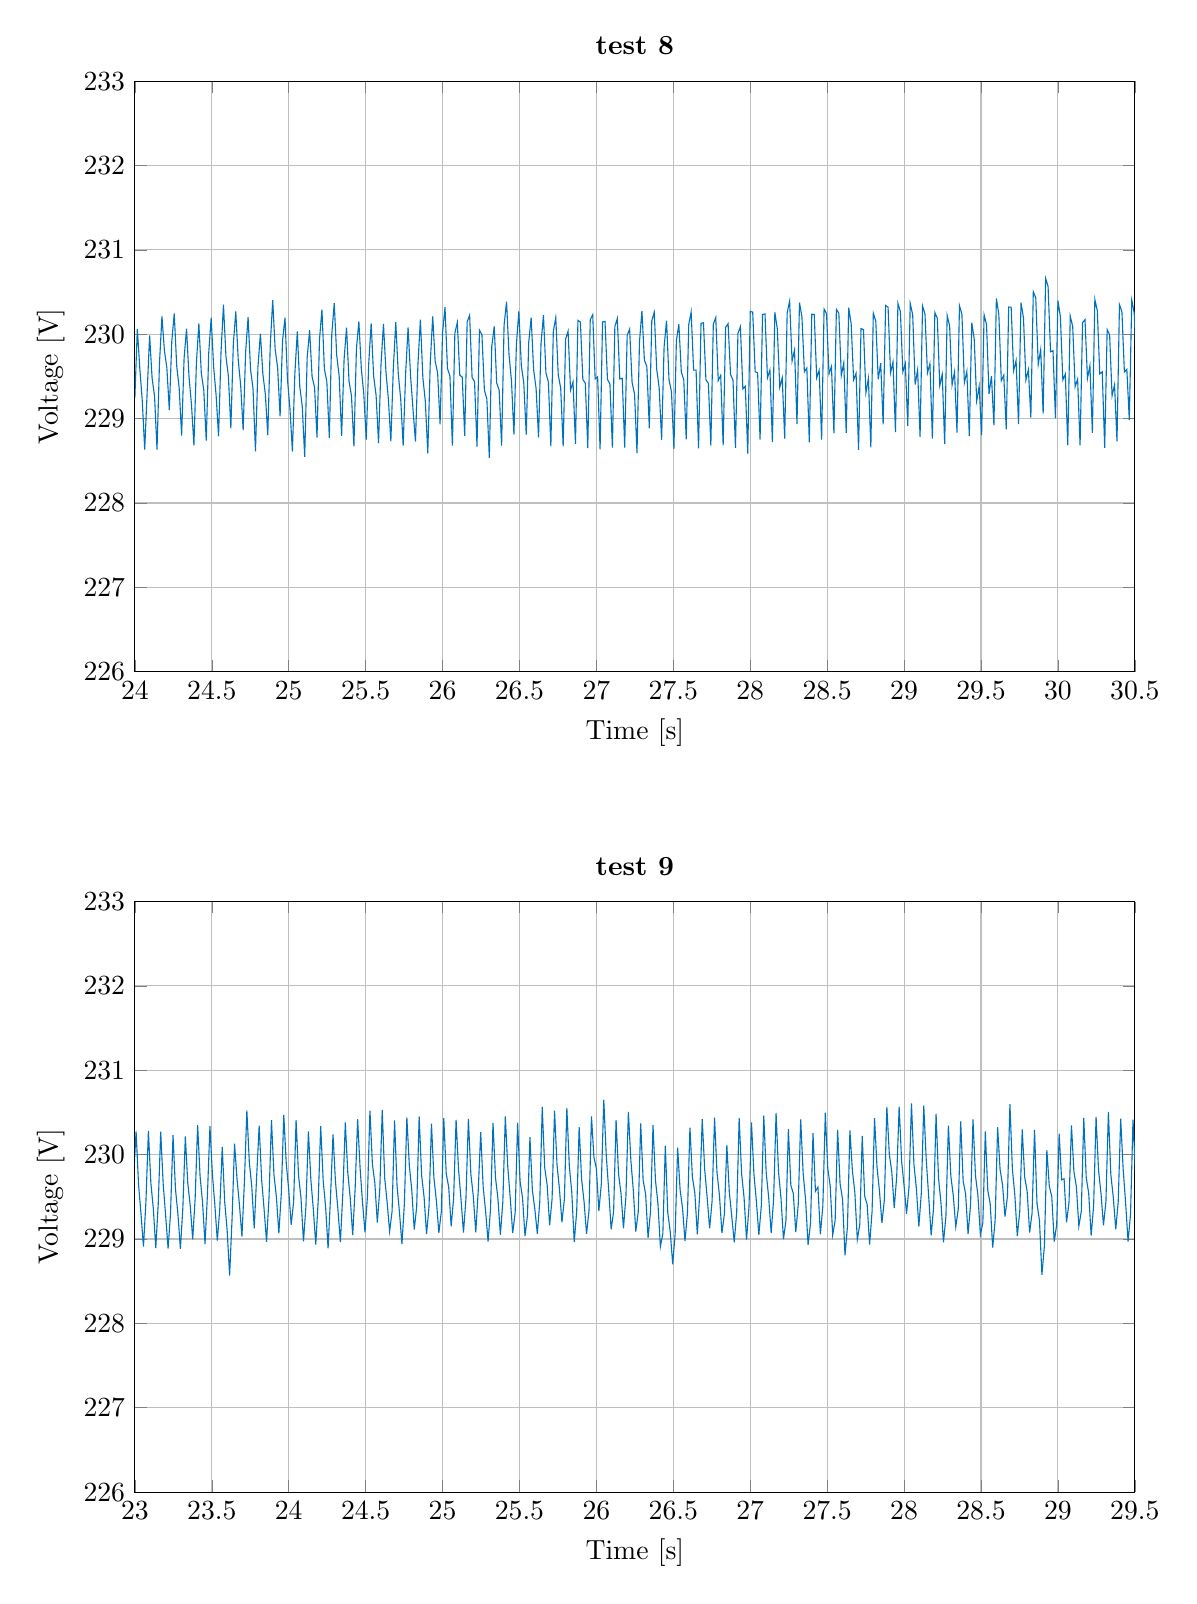
\begin{tikzpicture}

\begin{axis}[%
width=5in,
height=2.953in,
at={(1.142in,5.054in)},
scale only axis,
xmin=24,
xmax=30.5,
xlabel={Time [s]},
xmajorgrids,
ymin=226,
ymax=233,
ylabel={Voltage [V]},
ymajorgrids,
axis background/.style={fill=white},
title style={font=\bfseries},
title={test 8}
]
\addplot [color=mycolor1,solid,forget plot]
  table[row sep=crcr]{%
24	229.245265921995\\
24.016	230.063177722537\\
24.032	229.599759201865\\
24.048	229.215392681505\\
24.064	228.63317962675\\
24.08	229.316909651675\\
24.096	229.984674859096\\
24.112	229.481345336619\\
24.128	229.262980942599\\
24.144	228.632891151849\\
24.16	229.654450646327\\
24.176	230.211952810946\\
24.192	229.808758139791\\
24.208	229.600333375737\\
24.224	229.099669125591\\
24.24	229.914271820836\\
24.256	230.245498948148\\
24.272	229.624515241211\\
24.288	229.36378459628\\
24.304	228.799285275565\\
24.32	229.715668006143\\
24.336	230.064822815609\\
24.352	229.497208474902\\
24.368	229.166641486987\\
24.384	228.682880836958\\
24.4	229.660663396228\\
24.416	230.127240550322\\
24.432	229.537017288117\\
24.448	229.336196342122\\
24.464	228.738103493305\\
24.48	229.77533622273\\
24.496	230.194386247114\\
24.512	229.614321774269\\
24.528	229.281738179364\\
24.544	228.789853134609\\
24.56	229.784109608172\\
24.576	230.349825994116\\
24.592	229.739693032621\\
24.608	229.501680617981\\
24.624	228.883594559245\\
24.64	229.880357174041\\
24.656	230.269234415649\\
24.672	229.694756301554\\
24.688	229.38761371397\\
24.704	228.863060592665\\
24.72	229.7885292486\\
24.736	230.201317784605\\
24.752	229.58338864003\\
24.768	229.355882957416\\
24.784	228.610851691358\\
24.8	229.610917260346\\
24.816	230.007230149982\\
24.832	229.528222362182\\
24.848	229.292868744226\\
24.864	228.802975851939\\
24.88	229.863670229343\\
24.896	230.404225249665\\
24.912	229.82011088978\\
24.928	229.606750796352\\
24.944	229.026146908659\\
24.96	229.926721648429\\
24.976	230.196504086922\\
24.992	229.462143472648\\
25.008	229.124638993524\\
25.024	228.607791658258\\
25.04	229.531384440665\\
25.056	230.034002237939\\
25.072	229.37898902935\\
25.088	229.147790159789\\
25.104	228.545262801536\\
25.12	229.721537484445\\
25.136	230.046832867409\\
25.152	229.495376979801\\
25.168	229.371078085441\\
25.184	228.775049833452\\
25.2	229.934442615864\\
25.216	230.291153836497\\
25.232	229.58660911682\\
25.248	229.437619711306\\
25.264	228.773048774187\\
25.28	229.998797491315\\
25.296	230.368371274505\\
25.312	229.750825322978\\
25.328	229.50583993811\\
25.344	228.794552554726\\
25.36	229.702953897657\\
25.376	230.078262735494\\
25.392	229.445601401081\\
25.408	229.271026539571\\
25.424	228.67195704983\\
25.44	229.820016681104\\
25.456	230.152850943207\\
25.472	229.592850038769\\
25.488	229.294424123797\\
25.504	228.751203079201\\
25.52	229.647063103007\\
25.536	230.128349466368\\
25.552	229.504444853003\\
25.568	229.276078849304\\
25.584	228.709725831456\\
25.6	229.642560366372\\
25.616	230.12208733411\\
25.632	229.560628523238\\
25.648	229.227250820156\\
25.664	228.73090004437\\
25.68	229.593904389879\\
25.696	230.142482834352\\
25.712	229.536729334777\\
25.728	229.231775598469\\
25.744	228.678376580766\\
25.76	229.530416064251\\
25.776	230.081173035413\\
25.792	229.506573988006\\
25.808	229.108062666506\\
25.824	228.728805928706\\
25.84	229.644249145134\\
25.856	230.174097863217\\
25.872	229.485619327716\\
25.888	229.206468084654\\
25.904	228.589147944812\\
25.92	229.654871620914\\
25.936	230.212511295602\\
25.952	229.682119134575\\
25.968	229.540094382044\\
25.984	228.932915866676\\
26	230.016939978006\\
26.016	230.319953454918\\
26.032	229.593701062246\\
26.048	229.503898468478\\
26.064	228.680706915173\\
26.08	230.010927557841\\
26.096	230.139741895135\\
26.112	229.514543960678\\
26.128	229.492075574654\\
26.144	228.795890303662\\
26.16	230.146266733805\\
26.176	230.225813292665\\
26.192	229.486199657382\\
26.208	229.438929239744\\
26.224	228.66735789413\\
26.24	230.047441266544\\
26.256	229.994313286387\\
26.272	229.336750457637\\
26.288	229.232846045569\\
26.304	228.534633940943\\
26.32	229.856410522602\\
26.336	230.092100771852\\
26.352	229.420627313291\\
26.368	229.337630622454\\
26.384	228.67837739864\\
26.4	230.108398114999\\
26.416	230.384383430934\\
26.432	229.760329460818\\
26.448	229.449184856085\\
26.464	228.81158330712\\
26.48	229.876581881571\\
26.496	230.271803942793\\
26.512	229.627428750456\\
26.528	229.424186426401\\
26.544	228.811515254872\\
26.56	229.9014546384\\
26.576	230.196429869535\\
26.592	229.580406759678\\
26.608	229.359002476543\\
26.624	228.776170737518\\
26.64	229.887176932013\\
26.656	230.226428693805\\
26.672	229.540700132353\\
26.688	229.432379126659\\
26.704	228.672017628985\\
26.72	230.032562022643\\
26.736	230.197028442676\\
26.752	229.51712370952\\
26.768	229.362464964578\\
26.784	228.669773828869\\
26.8	229.942662021192\\
26.816	230.03544474999\\
26.832	229.338245873708\\
26.848	229.43420704752\\
26.864	228.700648103888\\
26.88	230.163973902576\\
26.896	230.143176668584\\
26.912	229.463481944178\\
26.928	229.418742496735\\
26.944	228.648859745535\\
26.96	230.169585273373\\
26.976	230.231973856645\\
26.992	229.469354763132\\
27.008	229.496307680022\\
27.024	228.634754656642\\
27.04	230.146258112746\\
27.056	230.15128427043\\
27.072	229.4640495572\\
27.088	229.411185335505\\
27.104	228.654780635253\\
27.12	230.091072994115\\
27.136	230.186619923754\\
27.152	229.470434442354\\
27.168	229.477273240413\\
27.184	228.656430162875\\
27.2	229.985156369043\\
27.216	230.060813623724\\
27.232	229.428627180736\\
27.248	229.291027249699\\
27.264	228.590082064299\\
27.28	229.904774430632\\
27.296	230.277526591686\\
27.312	229.693666824797\\
27.328	229.616568794012\\
27.344	228.885248008597\\
27.36	230.15816070824\\
27.376	230.261055959743\\
27.392	229.587644590939\\
27.408	229.364312335245\\
27.424	228.74721842548\\
27.44	229.84670963365\\
27.456	230.161797489442\\
27.472	229.458812689826\\
27.488	229.318999187899\\
27.504	228.64136097046\\
27.52	229.922654848816\\
27.536	230.119467873246\\
27.552	229.552695901742\\
27.568	229.459809944633\\
27.584	228.754157290294\\
27.6	230.113776815739\\
27.616	230.263030930312\\
27.632	229.574526791566\\
27.648	229.574716298302\\
27.664	228.64790762092\\
27.68	230.129659477411\\
27.696	230.135412305581\\
27.712	229.461309299234\\
27.728	229.416916118778\\
27.744	228.680927462897\\
27.76	230.119291596554\\
27.776	230.197987806235\\
27.792	229.45025896258\\
27.808	229.513410101831\\
27.824	228.683691628249\\
27.84	230.080517482882\\
27.856	230.125568464404\\
27.872	229.523284549046\\
27.888	229.456431911978\\
27.904	228.652177267776\\
27.92	230.006876479975\\
27.936	230.08915830414\\
27.952	229.351947456077\\
27.968	229.38122835873\\
27.984	228.58350766634\\
28	230.270120972443\\
28.016	230.262315138593\\
28.032	229.557144400276\\
28.048	229.541036510491\\
28.064	228.75213721456\\
28.08	230.233635603747\\
28.096	230.240426077588\\
28.112	229.482423047125\\
28.128	229.575255635361\\
28.144	228.72239652592\\
28.16	230.261472905052\\
28.176	230.06208826996\\
28.192	229.370533530853\\
28.208	229.484043550068\\
28.224	228.763788281488\\
28.24	230.252688232468\\
28.256	230.392559344641\\
28.272	229.682598867136\\
28.288	229.811482560674\\
28.304	228.93594405397\\
28.32	230.375053897318\\
28.336	230.207559030152\\
28.352	229.554624826719\\
28.368	229.5988401796\\
28.384	228.719271662339\\
28.4	230.236558728296\\
28.416	230.235271753536\\
28.432	229.483596944167\\
28.448	229.572001588709\\
28.464	228.750564409868\\
28.48	230.298489260166\\
28.496	230.244334127497\\
28.512	229.530903988431\\
28.528	229.616898138167\\
28.544	228.824163591103\\
28.56	230.294492772578\\
28.576	230.248081341741\\
28.592	229.509693525369\\
28.608	229.659951606413\\
28.624	228.829676219761\\
28.64	230.314215673083\\
28.656	230.125621888945\\
28.672	229.460306938745\\
28.688	229.536321347345\\
28.704	228.629234080929\\
28.72	230.066582725982\\
28.736	230.055619889259\\
28.752	229.305588010573\\
28.768	229.475006807758\\
28.784	228.659428600684\\
28.8	230.249436262634\\
28.816	230.156047999505\\
28.832	229.466697146916\\
28.848	229.656428827647\\
28.864	228.930221463487\\
28.88	230.340485805302\\
28.896	230.320909191273\\
28.912	229.541554728837\\
28.928	229.671084903307\\
28.944	228.839400555954\\
28.96	230.364502647183\\
28.976	230.268259035179\\
28.992	229.553606820961\\
29.008	229.652071469906\\
29.024	228.914546095504\\
29.04	230.364521335861\\
29.056	230.230458469489\\
29.072	229.402999388548\\
29.088	229.578375507914\\
29.104	228.784823393608\\
29.12	230.33551656184\\
29.136	230.236508433932\\
29.152	229.540689429806\\
29.168	229.65123491823\\
29.184	228.762842160475\\
29.2	230.258178084414\\
29.216	230.188098693202\\
29.232	229.390217316209\\
29.248	229.525048117062\\
29.264	228.696898530101\\
29.28	230.222875293319\\
29.296	230.101092142756\\
29.312	229.398481761162\\
29.328	229.554149078892\\
29.344	228.833150450649\\
29.36	230.338239124634\\
29.376	230.235174082714\\
29.392	229.425965459325\\
29.408	229.559265593323\\
29.424	228.792638634319\\
29.44	230.135376525779\\
29.456	229.94219450794\\
29.472	229.209049237513\\
29.488	229.38292104546\\
29.504	228.803665238984\\
29.52	230.230923459492\\
29.536	230.115984922409\\
29.552	229.290560508836\\
29.568	229.503929392379\\
29.584	228.91977263586\\
29.6	230.423501885845\\
29.616	230.233581907843\\
29.632	229.448253270138\\
29.648	229.514351027579\\
29.664	228.871634614272\\
29.68	230.322018390824\\
29.696	230.321584641798\\
29.712	229.568575468025\\
29.728	229.686956545635\\
29.744	228.93469033075\\
29.76	230.374667659564\\
29.776	230.195406339921\\
29.792	229.45934339347\\
29.808	229.578223715117\\
29.824	229.010358484235\\
29.84	230.503892521813\\
29.856	230.432010003218\\
29.872	229.641767494276\\
29.888	229.81686778318\\
29.904	229.057727238026\\
29.92	230.66192187681\\
29.936	230.567357028015\\
29.952	229.791537644857\\
29.968	229.8042501119\\
29.984	229.002084063501\\
30	230.398901348363\\
30.016	230.208966675007\\
30.032	229.458639700601\\
30.048	229.526007812503\\
30.064	228.68481314895\\
30.08	230.213788102316\\
30.096	230.092385731796\\
30.112	229.378080662134\\
30.128	229.467096288622\\
30.144	228.681991448146\\
30.16	230.135845423164\\
30.176	230.172209172349\\
30.192	229.476941403285\\
30.208	229.626820744654\\
30.224	228.832220708436\\
30.24	230.412584349082\\
30.256	230.279404206535\\
30.272	229.531042742327\\
30.288	229.553979593962\\
30.304	228.651886107534\\
30.32	230.05357361655\\
30.336	229.993669904286\\
30.352	229.270476704834\\
30.368	229.40003416493\\
30.384	228.729238250473\\
30.4	230.35053326485\\
30.416	230.2654273441\\
30.432	229.553999729631\\
30.448	229.582891931627\\
30.464	228.982381676217\\
30.48	230.405511036624\\
30.496	230.250499041306\\
30.512	229.524127922526\\
};
\end{axis}

\begin{axis}[%
width=5in,
height=2.953in,
at={(1.142in,0.952in)},
scale only axis,
xmin=23,
xmax=29.5,
xlabel={Time [s]},
xmajorgrids,
ymin=226,
ymax=233,
ylabel={Voltage [V]},
ymajorgrids,
axis background/.style={fill=white},
title style={font=\bfseries},
title={test 9}
]
\addplot [color=mycolor1,solid,forget plot]
  table[row sep=crcr]{%
22.992	229.744562833884\\
23.008	230.274722192548\\
23.024	229.643112535352\\
23.04	229.296329055193\\
23.056	228.909387491723\\
23.072	229.444680679176\\
23.088	230.281844188903\\
23.104	229.663816360788\\
23.12	229.359922764415\\
23.136	228.891277784599\\
23.152	229.418487312459\\
23.168	230.271558674731\\
23.184	229.653673223111\\
23.2	229.281181596003\\
23.216	228.886209425239\\
23.232	229.308989286496\\
23.248	230.230936290656\\
23.264	229.590959238949\\
23.28	229.29374319471\\
23.296	228.88246491041\\
23.312	229.369995708793\\
23.328	230.216459745689\\
23.344	229.661176770622\\
23.36	229.396148560683\\
23.376	228.996419560204\\
23.392	229.485748145661\\
23.408	230.349232929592\\
23.424	229.741605162783\\
23.44	229.435204189526\\
23.456	228.940825635772\\
23.472	229.535879663539\\
23.488	230.337699557524\\
23.504	229.770141315686\\
23.52	229.402190589267\\
23.536	228.980597017484\\
23.552	229.357907033732\\
23.568	230.0922763926\\
23.584	229.440100764411\\
23.6	229.097990819807\\
23.616	228.56701192695\\
23.632	229.245939297454\\
23.648	230.130463178879\\
23.664	229.713560767595\\
23.68	229.401418444348\\
23.696	229.02867167634\\
23.712	229.675020336932\\
23.728	230.524304553957\\
23.744	229.911027116334\\
23.76	229.618218101856\\
23.776	229.126340076831\\
23.792	229.753347530037\\
23.808	230.342449563101\\
23.824	229.704987514548\\
23.84	229.354170612814\\
23.856	228.965350508169\\
23.872	229.488740291037\\
23.888	230.407155522187\\
23.904	229.764997743597\\
23.92	229.499024766459\\
23.936	229.066858002896\\
23.952	229.541680190199\\
23.968	230.471136137992\\
23.984	229.901324343991\\
24	229.585133417817\\
24.016	229.168591995797\\
24.032	229.439681529636\\
24.048	230.40873437842\\
24.064	229.752176422974\\
24.08	229.482356262128\\
24.096	228.971123586711\\
24.112	229.386358493423\\
24.128	230.275462026569\\
24.144	229.704568650044\\
24.16	229.35374700588\\
24.176	228.934897903918\\
24.192	229.463681125979\\
24.208	230.337589696401\\
24.224	229.696203214719\\
24.24	229.3765431823\\
24.256	228.888433785013\\
24.272	229.501757212532\\
24.288	230.241088745253\\
24.304	229.678841473423\\
24.32	229.347778074755\\
24.336	228.964047436545\\
24.352	229.546722686817\\
24.368	230.380601589777\\
24.384	229.785815593764\\
24.4	229.484580748377\\
24.416	229.044857655185\\
24.432	229.601121149629\\
24.448	230.419565021754\\
24.464	229.842064454738\\
24.48	229.426621875151\\
24.496	229.079624687395\\
24.512	229.509810251243\\
24.528	230.522393258269\\
24.544	229.888322539219\\
24.56	229.661080150106\\
24.576	229.193903070768\\
24.592	229.588159696648\\
24.608	230.530641375117\\
24.624	229.718733501807\\
24.64	229.431452462659\\
24.656	229.090124611272\\
24.672	229.328170472303\\
24.688	230.405184949382\\
24.704	229.635214197438\\
24.72	229.316363740004\\
24.736	228.939071833151\\
24.752	229.423035105657\\
24.768	230.441232590184\\
24.784	229.873500930722\\
24.8	229.57878485908\\
24.816	229.110803747819\\
24.832	229.383192251899\\
24.848	230.452167656391\\
24.864	229.75463873367\\
24.88	229.496826460402\\
24.896	229.059651785749\\
24.912	229.378431683787\\
24.928	230.368194745555\\
24.944	229.72412334369\\
24.96	229.452748903862\\
24.976	229.072434684854\\
24.992	229.321561530697\\
25.008	230.430912527393\\
25.024	229.774290297196\\
25.04	229.614558347494\\
25.056	229.150818373112\\
25.072	229.483459667265\\
25.088	230.41299410014\\
25.104	229.822620690457\\
25.12	229.471272156274\\
25.136	229.07597250432\\
25.152	229.472029383294\\
25.168	230.423133802337\\
25.184	229.769794295469\\
25.2	229.507759321367\\
25.216	229.077935165021\\
25.232	229.570790603722\\
25.248	230.266710365499\\
25.264	229.618213657596\\
25.28	229.327337648998\\
25.296	228.969419340049\\
25.312	229.360109181429\\
25.328	230.37528673024\\
25.344	229.731214438047\\
25.36	229.478611905569\\
25.376	229.050218398803\\
25.392	229.446024028332\\
25.408	230.453506449534\\
25.424	229.856237501776\\
25.44	229.488677546965\\
25.456	229.069516478139\\
25.472	229.312930509687\\
25.488	230.379774855237\\
25.504	229.682080610837\\
25.52	229.486492577132\\
25.536	229.033498175785\\
25.552	229.27953422425\\
25.568	230.205702062223\\
25.584	229.573910471045\\
25.6	229.353266687588\\
25.616	229.06241345865\\
25.632	229.440513831225\\
25.648	230.564392545695\\
25.664	229.846423744161\\
25.68	229.64020298951\\
25.696	229.162470640074\\
25.712	229.475400704704\\
25.728	230.521180190979\\
25.744	229.881113451857\\
25.76	229.590684786486\\
25.776	229.1986857862\\
25.792	229.473703829583\\
25.808	230.554304350046\\
25.824	229.865198561069\\
25.84	229.555770931744\\
25.856	228.962719551041\\
25.872	229.329796119532\\
25.888	230.325367900549\\
25.904	229.706989658666\\
25.92	229.439852560358\\
25.936	229.061263649724\\
25.952	229.337599915946\\
25.968	230.453977237061\\
25.984	229.968677478513\\
26	229.835687837113\\
26.016	229.331704070147\\
26.032	229.649766426131\\
26.048	230.649512806468\\
26.064	229.996058676601\\
26.08	229.579393277507\\
26.096	229.11327318021\\
26.112	229.326617538969\\
26.128	230.409963285219\\
26.144	229.769445231065\\
26.16	229.539858994835\\
26.176	229.127290254328\\
26.192	229.505130454072\\
26.208	230.506415753596\\
26.224	229.934545628773\\
26.24	229.575669203105\\
26.256	229.088758387242\\
26.272	229.318551109584\\
26.288	230.369339155497\\
26.304	229.692714727062\\
26.32	229.531614443153\\
26.336	229.01297876529\\
26.352	229.329621598956\\
26.368	230.349097622582\\
26.384	229.695471782447\\
26.4	229.421327422204\\
26.416	228.90945452478\\
26.432	229.064478073174\\
26.448	230.106777616189\\
26.464	229.311614538287\\
26.48	229.087888992024\\
26.496	228.699664683705\\
26.512	229.062094302671\\
26.528	230.08230337296\\
26.544	229.586607562511\\
26.56	229.363381943282\\
26.576	228.975037489792\\
26.592	229.308823494041\\
26.608	230.320723029556\\
26.624	229.734094023787\\
26.64	229.544422396245\\
26.656	229.055166065312\\
26.672	229.54289835069\\
26.688	230.420742464582\\
26.704	229.821740083276\\
26.72	229.494278846718\\
26.736	229.124987305467\\
26.752	229.448468639056\\
26.768	230.437546190237\\
26.784	229.78772483507\\
26.8	229.515360984182\\
26.816	229.070228287398\\
26.832	229.293681530763\\
26.848	230.113631982252\\
26.864	229.557034709703\\
26.88	229.266210471543\\
26.896	228.961275124922\\
26.912	229.316894807223\\
26.928	230.433326426114\\
26.944	229.771931294604\\
26.96	229.488675115594\\
26.976	228.992906951732\\
26.992	229.385151169148\\
27.008	230.382327220945\\
27.024	229.768989502239\\
27.04	229.447644890912\\
27.056	229.04823708114\\
27.072	229.391950110206\\
27.088	230.461881524211\\
27.104	229.778985488678\\
27.12	229.490706746686\\
27.136	229.069913361108\\
27.152	229.471258721091\\
27.168	230.493299149983\\
27.184	229.792885198643\\
27.2	229.483556768089\\
27.216	228.997578390226\\
27.232	229.216054874605\\
27.248	230.302811323958\\
27.264	229.63525390568\\
27.28	229.53937564587\\
27.296	229.08100991406\\
27.312	229.406900010493\\
27.328	230.418213507705\\
27.344	229.777109847034\\
27.36	229.458649014349\\
27.376	228.929383228578\\
27.392	229.189327065687\\
27.408	230.254504231916\\
27.424	229.565746014779\\
27.44	229.615973016885\\
27.456	229.055512642896\\
27.472	229.393406203574\\
27.488	230.4966594352\\
27.504	229.8360566595\\
27.52	229.625720151534\\
27.536	229.046504518821\\
27.552	229.221276754417\\
27.568	230.291756937354\\
27.584	229.656474780499\\
27.6	229.47285303361\\
27.616	228.806140119375\\
27.632	229.148582429299\\
27.648	230.286335047529\\
27.664	229.810244482161\\
27.68	229.55092837006\\
27.696	228.992864601351\\
27.712	229.170755019213\\
27.728	230.220804609\\
27.744	229.506924564606\\
27.76	229.409787181206\\
27.776	228.933598076752\\
27.792	229.325579530765\\
27.808	230.432551635378\\
27.824	229.853050124606\\
27.84	229.569939271932\\
27.856	229.189045197209\\
27.872	229.466006326625\\
27.888	230.567054398189\\
27.904	230.007980698945\\
27.92	229.796612475025\\
27.936	229.366158309185\\
27.952	229.738805011654\\
27.968	230.568072015791\\
27.984	229.920934563309\\
28	229.63332226453\\
28.016	229.298215373656\\
28.032	229.613279646241\\
28.048	230.607318165008\\
28.064	229.886427019964\\
28.08	229.597657947163\\
28.096	229.147072040075\\
28.112	229.542494163807\\
28.128	230.579684795372\\
28.144	229.940502903204\\
28.16	229.502754983067\\
28.176	229.043144561365\\
28.192	229.373403455129\\
28.208	230.484200512243\\
28.224	229.720724903682\\
28.24	229.424359762491\\
28.256	228.959180046151\\
28.272	229.26764367319\\
28.288	230.344122140831\\
28.304	229.745600284096\\
28.32	229.510064224939\\
28.336	229.143148824031\\
28.352	229.352299356354\\
28.368	230.393843722799\\
28.384	229.684484417829\\
28.4	229.533088335693\\
28.416	229.059355107853\\
28.432	229.403016839229\\
28.448	230.416328303772\\
28.464	229.751291633178\\
28.48	229.51787276235\\
28.496	229.05178633046\\
28.512	229.191688795389\\
28.528	230.273927886429\\
28.544	229.579940679599\\
28.56	229.413056607012\\
28.576	228.896901704231\\
28.592	229.225271694597\\
28.608	230.325029793622\\
28.624	229.825319253833\\
28.64	229.641919043118\\
28.656	229.265137422392\\
28.672	229.506872650606\\
28.688	230.598913410325\\
28.704	229.82971139384\\
28.72	229.518773951767\\
28.736	229.033317877643\\
28.752	229.331131736282\\
28.768	230.297846329231\\
28.784	229.731296679078\\
28.8	229.564073257738\\
28.816	229.077124492344\\
28.832	229.305980746634\\
28.848	230.292397554011\\
28.864	229.421437332361\\
28.88	229.218632614531\\
28.896	228.574823607491\\
28.912	228.915680305461\\
28.928	230.053525251211\\
28.944	229.625059485281\\
28.96	229.502599146633\\
28.976	228.968403191905\\
28.992	229.170394560103\\
29.008	230.249691034609\\
29.024	229.700231918349\\
29.04	229.714463264114\\
29.056	229.197572825573\\
29.072	229.430262425114\\
29.088	230.346481816215\\
29.104	229.796303879213\\
29.12	229.62078435002\\
29.136	229.151033101052\\
29.152	229.329602759757\\
29.168	230.434031925925\\
29.184	229.728424790976\\
29.2	229.543536364095\\
29.216	229.039481987861\\
29.232	229.389616912657\\
29.248	230.4465482418\\
29.264	229.817519361988\\
29.28	229.539137389322\\
29.296	229.162770257704\\
29.312	229.441562994725\\
29.328	230.5077748082\\
29.344	229.760975383892\\
29.36	229.493773546587\\
29.376	229.114609254066\\
29.392	229.443796618885\\
29.408	230.426810635472\\
29.424	229.828597113987\\
29.44	229.428916443887\\
29.456	228.969145475214\\
29.472	229.294816048476\\
29.488	230.415510498302\\
29.504	229.779042165368\\
};
\end{axis}
\end{tikzpicture}%
\caption{Steady state Voltage output of the genset at 30 kW load.}
\label{fig:test8-9steadyvolt30kw}
\end{figure}

\begin{figure}[H]
\centering
% This file was created by matlab2tikz.
%
%The latest updates can be retrieved from
%  http://www.mathworks.com/matlabcentral/fileexchange/22022-matlab2tikz-matlab2tikz
%where you can also make suggestions and rate matlab2tikz.
%
\definecolor{mycolor1}{rgb}{0.00000,0.44700,0.74100}%
%
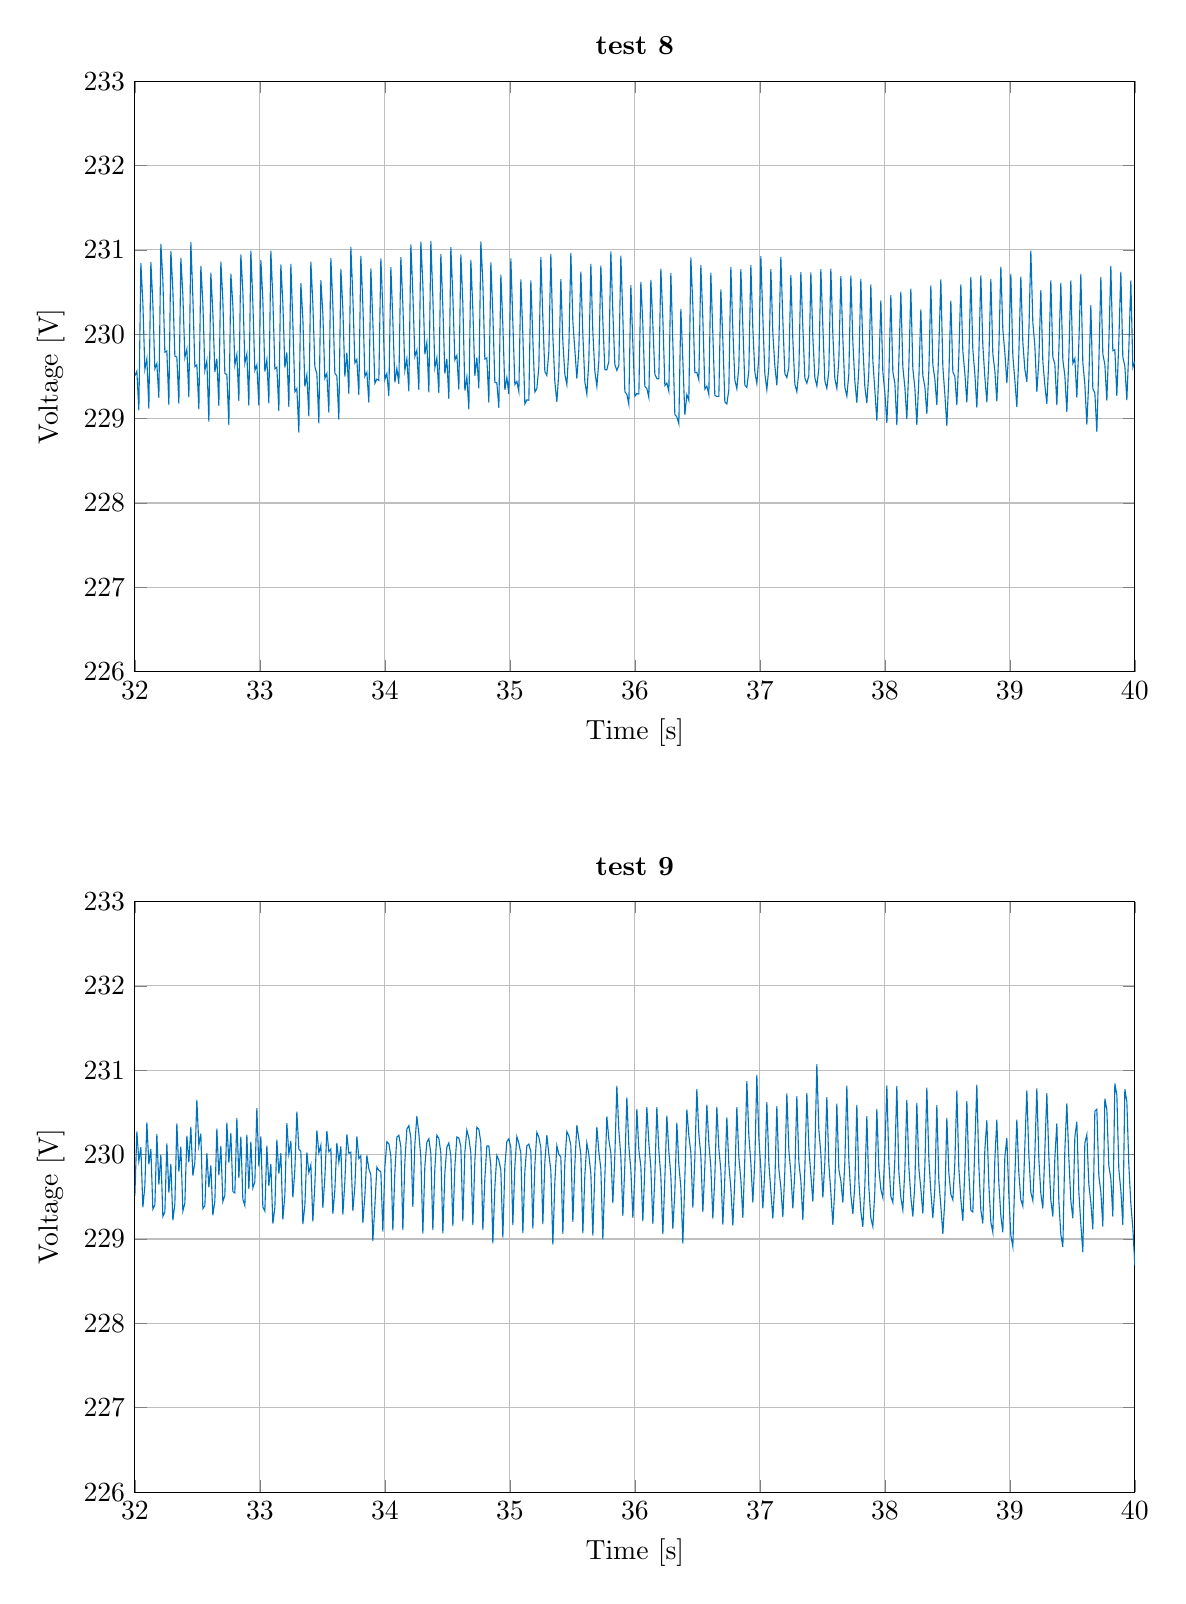
\begin{tikzpicture}

\begin{axis}[%
width=5in,
height=2.953in,
at={(1.142in,5.054in)},
scale only axis,
xmin=32,
xmax=40,
xlabel={Time [s]},
xmajorgrids,
ymin=226,
ymax=233,
ylabel={Voltage [V]},
ymajorgrids,
axis background/.style={fill=white},
title style={font=\bfseries},
title={test 8}
]
\addplot [color=mycolor1,solid,forget plot]
  table[row sep=crcr]{%
32	229.507324809836\\
32.016	229.561473486473\\
32.032	229.097425673036\\
32.048	230.842246710692\\
32.064	230.372239174047\\
32.08	229.585297527207\\
32.096	229.706898712043\\
32.112	229.119661821145\\
32.128	230.856137244166\\
32.144	230.358967351133\\
32.16	229.590155569482\\
32.176	229.650993472035\\
32.192	229.244573421722\\
32.208	231.070529523768\\
32.224	230.645481981368\\
32.24	229.786372951373\\
32.256	229.801314302602\\
32.272	229.163535029118\\
32.288	230.988523814323\\
32.304	230.518844458954\\
32.32	229.739980300256\\
32.336	229.729511851887\\
32.352	229.178222307581\\
32.368	230.904257980709\\
32.384	230.467505074953\\
32.4	229.722435928666\\
32.416	229.822242629718\\
32.432	229.252952119771\\
32.448	231.093437847172\\
32.464	230.439339594977\\
32.48	229.61616540904\\
32.496	229.636310180681\\
32.512	229.108718604408\\
32.528	230.811220297232\\
32.544	230.369209876657\\
32.56	229.569076794687\\
32.576	229.684339271838\\
32.592	228.965255834394\\
32.608	230.729725057307\\
32.624	230.249196348702\\
32.64	229.551471793731\\
32.656	229.709572489058\\
32.672	229.150712443887\\
32.688	230.858956346478\\
32.704	230.401030545331\\
32.72	229.534376592341\\
32.736	229.523197312031\\
32.752	228.923632310195\\
32.768	230.71806283074\\
32.784	230.338830779634\\
32.8	229.635205049179\\
32.816	229.756809206232\\
32.832	229.209545699927\\
32.848	230.946888819191\\
32.864	230.503340760712\\
32.88	229.655503435116\\
32.896	229.765862799726\\
32.912	229.15266688596\\
32.928	230.991562004419\\
32.944	230.374011020781\\
32.96	229.570960053888\\
32.976	229.635375164717\\
32.992	229.153372943331\\
33.008	230.878087395437\\
33.024	230.404475398954\\
33.04	229.558177019718\\
33.056	229.697774917463\\
33.072	229.181498552221\\
33.088	230.98992361351\\
33.104	230.4137365154\\
33.12	229.590440124057\\
33.136	229.608958338756\\
33.152	229.090248126613\\
33.168	230.826149373222\\
33.184	230.366506328678\\
33.2	229.604690042802\\
33.216	229.782869489617\\
33.232	229.138112499621\\
33.248	230.832923804086\\
33.264	230.131156056356\\
33.28	229.318004461862\\
33.296	229.355498938059\\
33.312	228.835188103803\\
33.328	230.604543317428\\
33.344	230.186194244532\\
33.36	229.378859022557\\
33.376	229.517741769315\\
33.392	229.027856390646\\
33.408	230.859524437982\\
33.424	230.356533583983\\
33.44	229.615805850585\\
33.456	229.530859805878\\
33.472	228.944692263905\\
33.488	230.640177210434\\
33.504	230.241779239344\\
33.52	229.477634744659\\
33.536	229.535095757091\\
33.552	229.071802984699\\
33.568	230.902446443896\\
33.584	230.349282709175\\
33.6	229.537965601323\\
33.616	229.504599873747\\
33.632	228.987505613866\\
33.648	230.77521246034\\
33.664	230.301424750466\\
33.68	229.498883867334\\
33.696	229.780097925808\\
33.712	229.294078850398\\
33.728	231.033600279961\\
33.744	230.440953976912\\
33.76	229.658920110473\\
33.776	229.700546910982\\
33.792	229.281610466912\\
33.808	230.92789146459\\
33.824	230.349819921364\\
33.84	229.498658433557\\
33.856	229.548186200844\\
33.872	229.189157154812\\
33.888	230.780581081055\\
33.904	230.14413377471\\
33.92	229.417818325206\\
33.936	229.46688369288\\
33.952	229.45250645649\\
33.968	230.900004778214\\
33.984	230.292633198243\\
34	229.461489631521\\
34.016	229.534120176855\\
34.032	229.267563609593\\
34.048	230.795428525012\\
34.064	230.159691478937\\
34.08	229.429001907365\\
34.096	229.593888905187\\
34.112	229.412131813256\\
34.128	230.913497399613\\
34.144	230.354070539005\\
34.16	229.572490373664\\
34.176	229.708802751966\\
34.192	229.323719225547\\
34.208	231.06573349533\\
34.224	230.480914225496\\
34.24	229.734264162007\\
34.256	229.810153186953\\
34.272	229.341219210351\\
34.288	231.097338031214\\
34.304	230.589956337617\\
34.32	229.76206335552\\
34.336	229.904950643152\\
34.352	229.312212145582\\
34.368	231.104781938103\\
34.384	230.433328112001\\
34.4	229.602421816397\\
34.416	229.718729721119\\
34.432	229.301585144535\\
34.448	230.951791724332\\
34.464	230.326583711084\\
34.48	229.532448471662\\
34.496	229.707993528656\\
34.512	229.234471472589\\
34.528	231.033488002896\\
34.544	230.442974339181\\
34.56	229.694840240379\\
34.576	229.748038811727\\
34.592	229.343201511884\\
34.608	230.944733236566\\
34.624	230.36039289203\\
34.64	229.331985864114\\
34.656	229.492037793348\\
34.672	229.109930005728\\
34.688	230.879856015933\\
34.704	230.28702868028\\
34.72	229.507061236155\\
34.736	229.723423717811\\
34.752	229.358136008321\\
34.768	231.099501640048\\
34.784	230.606035404788\\
34.8	229.705206832136\\
34.816	229.719330217397\\
34.832	229.188860990811\\
34.848	230.852765013264\\
34.864	230.235050122976\\
34.88	229.429670229777\\
34.896	229.42384092118\\
34.912	229.128412383877\\
34.928	230.706552121768\\
34.944	230.106184567985\\
34.96	229.34102952787\\
34.976	229.486798081526\\
34.992	229.289871651295\\
35.008	230.89850188542\\
35.024	230.138314435737\\
35.04	229.403546737792\\
35.056	229.439286475832\\
35.072	229.320875339214\\
35.088	230.650539099357\\
35.104	229.993860693885\\
35.12	229.173964536794\\
35.136	229.221975186427\\
35.152	229.217473975895\\
35.168	230.63697856776\\
35.184	229.936300122217\\
35.2	229.315566371398\\
35.216	229.354077863995\\
35.232	229.614481714265\\
35.248	230.912613229422\\
35.264	230.191336452062\\
35.28	229.559879808729\\
35.296	229.513464789571\\
35.312	229.793914005952\\
35.328	230.951143966108\\
35.344	229.979255581523\\
35.36	229.435371831159\\
35.376	229.199140219695\\
35.392	229.553811300971\\
35.408	230.652206464061\\
35.424	229.914323567947\\
35.44	229.524456153414\\
35.456	229.402052127513\\
35.472	229.830658915829\\
35.488	230.963264506254\\
35.504	230.151879582711\\
35.52	229.813788176651\\
35.536	229.474724750537\\
35.552	229.818843993785\\
35.568	230.742381359253\\
35.584	229.994441634548\\
35.6	229.43647613328\\
35.616	229.290005103145\\
35.632	229.687684149077\\
35.648	230.834501558999\\
35.664	230.02382929387\\
35.68	229.56070905821\\
35.696	229.382377620435\\
35.712	229.683746902991\\
35.728	230.814064240113\\
35.744	230.161578665081\\
35.76	229.579498700175\\
35.776	229.57909307917\\
35.792	229.67781884848\\
35.808	230.980476768034\\
35.824	230.262379730023\\
35.84	229.641481712458\\
35.856	229.571797597421\\
35.872	229.632112145898\\
35.888	230.929922316455\\
35.904	230.206273429789\\
35.92	229.31995766424\\
35.936	229.286120288761\\
35.952	229.168680781859\\
35.968	230.581503175353\\
35.984	229.890735519248\\
36	229.265589414764\\
36.016	229.296350662968\\
36.032	229.29086238657\\
36.048	230.620751672782\\
36.064	230.124660429797\\
36.08	229.382195049195\\
36.096	229.356075925845\\
36.112	229.250127462754\\
36.128	230.644846816885\\
36.144	230.115945711368\\
36.16	229.526702282375\\
36.176	229.473807769373\\
36.192	229.470575585994\\
36.208	230.777149573609\\
36.224	230.185023460398\\
36.24	229.391667455046\\
36.256	229.420272662533\\
36.272	229.32346095781\\
36.288	230.725848434977\\
36.304	229.895336006054\\
36.32	229.048451247772\\
36.336	229.019149483571\\
36.352	228.938665854591\\
36.368	230.301411591718\\
36.384	229.686146585262\\
36.4	229.044470385053\\
36.416	229.284745404456\\
36.432	229.215375411416\\
36.448	230.909894220954\\
36.464	230.338725928666\\
36.48	229.544444067775\\
36.496	229.547917319212\\
36.512	229.460450840887\\
36.528	230.818471719298\\
36.544	230.175487080518\\
36.56	229.349091289376\\
36.576	229.384430832959\\
36.592	229.28470522211\\
36.608	230.72931505403\\
36.624	229.997949376978\\
36.64	229.276411107836\\
36.656	229.26125329057\\
36.672	229.264546619808\\
36.688	230.531526026742\\
36.704	229.931524189475\\
36.72	229.198509004707\\
36.736	229.173986006671\\
36.752	229.343706387608\\
36.768	230.798072068997\\
36.784	230.051401806618\\
36.8	229.457912688875\\
36.816	229.353977855725\\
36.832	229.615957261868\\
36.848	230.771318395462\\
36.864	230.097586267943\\
36.88	229.397383302305\\
36.896	229.369517752545\\
36.912	229.569534940809\\
36.928	230.820765598854\\
36.944	230.061021238692\\
36.96	229.551671152022\\
36.976	229.415975758199\\
36.992	229.738009829633\\
37.008	230.925482762726\\
37.024	230.196936970281\\
37.04	229.530096733611\\
37.056	229.34308990118\\
37.072	229.608685841245\\
37.088	230.771106326742\\
37.104	230.011317074653\\
37.12	229.626765335506\\
37.136	229.395076648646\\
37.152	229.872958983262\\
37.168	230.915171483461\\
37.184	230.162267588283\\
37.2	229.532648727172\\
37.216	229.485478073813\\
37.232	229.610382938328\\
37.248	230.700747092452\\
37.264	229.93591919706\\
37.28	229.409659872104\\
37.296	229.317126998832\\
37.312	229.559418605595\\
37.328	230.734627001851\\
37.344	230.085052729564\\
37.36	229.481382649725\\
37.376	229.418215816826\\
37.392	229.512804729967\\
37.408	230.732580577571\\
37.424	229.966474744005\\
37.44	229.485179468382\\
37.456	229.387919268901\\
37.472	229.596061864375\\
37.488	230.771469644301\\
37.504	230.096012194922\\
37.52	229.445295524411\\
37.536	229.359344530488\\
37.552	229.565987995997\\
37.568	230.776234742932\\
37.584	229.998753640127\\
37.6	229.471899545249\\
37.616	229.357180920218\\
37.632	229.694492813244\\
37.648	230.68937585774\\
37.664	229.945815675566\\
37.68	229.373743597525\\
37.696	229.266771314768\\
37.712	229.529907092649\\
37.728	230.693352995743\\
37.744	229.910412002284\\
37.76	229.443601512754\\
37.776	229.188177513411\\
37.792	229.595856911845\\
37.808	230.654984624167\\
37.824	229.864086559169\\
37.84	229.377546592904\\
37.856	229.183114685363\\
37.872	229.554676659008\\
37.888	230.589172029726\\
37.904	229.684437115096\\
37.92	229.339663048231\\
37.936	228.975991646088\\
37.952	229.558729837764\\
37.968	230.399891266998\\
37.984	229.54967244646\\
38	229.310704462553\\
38.016	228.948316699181\\
38.032	229.493794137973\\
38.048	230.463885400193\\
38.064	229.554478643471\\
38.08	229.421591365581\\
38.096	228.923564372338\\
38.112	229.684726131654\\
38.128	230.503990474977\\
38.144	229.610669205954\\
38.16	229.37477139549\\
38.176	228.995010951056\\
38.192	229.618191706487\\
38.208	230.540799637172\\
38.224	229.590983013887\\
38.24	229.36746447383\\
38.256	228.925466436492\\
38.272	229.470357009843\\
38.288	230.29372681615\\
38.304	229.508667886123\\
38.32	229.380814440019\\
38.336	229.056160142468\\
38.352	229.568406982933\\
38.368	230.577743475683\\
38.384	229.638210573238\\
38.4	229.47058531235\\
38.416	229.160378741124\\
38.432	229.844406557928\\
38.448	230.650768330805\\
38.464	229.614281849607\\
38.48	229.287263175352\\
38.496	228.912875664388\\
38.512	229.50198424327\\
38.528	230.399345921628\\
38.544	229.554018507211\\
38.56	229.499569923223\\
38.576	229.160779421263\\
38.592	229.74062935805\\
38.608	230.590052166509\\
38.624	229.799010173424\\
38.64	229.538639081633\\
38.656	229.191735094208\\
38.672	229.719107182221\\
38.688	230.680730704741\\
38.704	229.81651017135\\
38.72	229.530259124315\\
38.736	229.13059949841\\
38.752	229.754289339852\\
38.768	230.696566368055\\
38.784	229.863560442784\\
38.8	229.493545198693\\
38.816	229.193415439781\\
38.832	229.688303497815\\
38.848	230.652680171075\\
38.864	229.765527740056\\
38.88	229.566151995155\\
38.896	229.204915411578\\
38.912	229.817843334139\\
38.928	230.801164300721\\
38.944	230.054763929054\\
38.96	229.784052461272\\
38.976	229.420709334915\\
38.992	229.817231304058\\
39.008	230.715885931469\\
39.024	229.746068999568\\
39.04	229.456976017923\\
39.056	229.138720332309\\
39.072	229.765098002652\\
39.088	230.681500291104\\
39.104	229.903402478707\\
39.12	229.584856230585\\
39.136	229.435995203013\\
39.152	230.018326561045\\
39.168	230.991593132511\\
39.184	230.135977059717\\
39.2	229.865297889892\\
39.216	229.31646726575\\
39.232	229.691443012522\\
39.248	230.523394525831\\
39.264	229.676320888783\\
39.28	229.396372388125\\
39.296	229.175920898319\\
39.312	229.698545802251\\
39.328	230.638118270646\\
39.344	229.728040470091\\
39.36	229.644495088092\\
39.376	229.160648681212\\
39.392	229.803113078478\\
39.408	230.606878669546\\
39.424	229.696752228217\\
39.44	229.508618992837\\
39.456	229.07838866377\\
39.472	229.730768493179\\
39.488	230.637131099763\\
39.504	229.652961195727\\
39.52	229.711204667235\\
39.536	229.248491781057\\
39.552	229.893485534319\\
39.568	230.714068771282\\
39.584	229.661693513799\\
39.6	229.405677895414\\
39.616	228.930063698661\\
39.632	229.469863609364\\
39.648	230.343372846111\\
39.664	229.354924226146\\
39.68	229.303500104376\\
39.696	228.843922628104\\
39.712	229.646278586951\\
39.728	230.67959552849\\
39.744	229.764420128356\\
39.76	229.641622615848\\
39.776	229.212303249346\\
39.792	229.899511257649\\
39.808	230.811023297839\\
39.824	229.803919814524\\
39.84	229.816573093917\\
39.856	229.268602203551\\
39.872	229.924564920391\\
39.888	230.737877769646\\
39.904	229.727185374924\\
39.92	229.62423940682\\
39.936	229.218677888105\\
39.952	229.828980538259\\
39.968	230.638082738127\\
39.984	229.603470877899\\
40	229.676312165151\\
40	229.676312165151\\
};
\end{axis}

\begin{axis}[%
width=5in,
height=2.953in,
at={(1.142in,0.952in)},
scale only axis,
xmin=32,
xmax=40,
xlabel={Time [s]},
xmajorgrids,
ymin=226,
ymax=233,
ylabel={Voltage [V]},
ymajorgrids,
axis background/.style={fill=white},
title style={font=\bfseries},
title={test 9}
]
\addplot [color=mycolor1,solid,forget plot]
  table[row sep=crcr]{%
32	229.510694613672\\
32.016	230.274637009024\\
32.032	229.923017800517\\
32.048	230.088200727098\\
32.064	229.374969903103\\
32.08	229.629141582753\\
32.096	230.382951924302\\
32.112	229.886043443045\\
32.128	230.066283383749\\
32.144	229.352564607773\\
32.16	229.402278028287\\
32.176	230.244202981272\\
32.192	229.643721181\\
32.208	230.000200295167\\
32.224	229.266689797247\\
32.24	229.31891887273\\
32.256	230.133642117978\\
32.272	229.548781928452\\
32.288	229.8879736916\\
32.304	229.221769861871\\
32.32	229.417784938727\\
32.336	230.371497609537\\
32.352	229.79764562533\\
32.368	230.095441773151\\
32.384	229.33131255821\\
32.4	229.425900662562\\
32.416	230.223310941058\\
32.432	229.908308011192\\
32.448	230.327537517811\\
32.464	229.75038318106\\
32.48	229.909704942478\\
32.496	230.649827344945\\
32.512	230.106146300418\\
32.528	230.249314694191\\
32.544	229.35966175207\\
32.56	229.395385558154\\
32.576	230.017351032945\\
32.592	229.612677927806\\
32.608	229.872552199588\\
32.624	229.281245455281\\
32.64	229.449020290912\\
32.656	230.307809593512\\
32.672	229.75441025532\\
32.688	230.101857971372\\
32.704	229.442257541641\\
32.72	229.518777093953\\
32.736	230.378786497755\\
32.752	229.90493611029\\
32.768	230.253837459391\\
32.784	229.561312278946\\
32.8	229.545805188978\\
32.816	230.434880716392\\
32.832	229.72038777666\\
32.848	230.213449650647\\
32.864	229.468534515384\\
32.88	229.395914520393\\
32.896	230.237287575697\\
32.912	229.591368237228\\
32.928	230.154655483133\\
32.944	229.605124818775\\
32.96	229.680229239754\\
32.976	230.550102182969\\
32.992	229.857990251244\\
33.008	230.214686466095\\
33.024	229.378248900646\\
33.04	229.330578588105\\
33.056	230.107523763814\\
33.072	229.629725009758\\
33.088	229.890316735273\\
33.104	229.181516661005\\
33.12	229.369362927295\\
33.136	230.176953708164\\
33.152	229.774196141103\\
33.168	230.016024817959\\
33.184	229.229768273798\\
33.2	229.52115195687\\
33.216	230.37248325275\\
33.232	230.005821329268\\
33.248	230.161793449296\\
33.264	229.492213274903\\
33.28	229.822042665999\\
33.296	230.508080844832\\
33.312	230.064271096533\\
33.328	230.040427438614\\
33.344	229.177313553994\\
33.36	229.395670408987\\
33.376	230.027345719755\\
33.392	229.787368887436\\
33.408	229.877403232408\\
33.424	229.206769238938\\
33.44	229.643841900954\\
33.456	230.286217564466\\
33.472	230.019091807988\\
33.488	230.112714260056\\
33.504	229.36985093677\\
33.52	229.726657102667\\
33.536	230.282221890234\\
33.552	230.035586455697\\
33.568	230.066785595684\\
33.584	229.298839161096\\
33.6	229.582381167666\\
33.616	230.139971281249\\
33.632	229.910557051475\\
33.648	230.098030870136\\
33.664	229.289551419059\\
33.68	229.679659417604\\
33.696	230.240816811952\\
33.712	230.01487290702\\
33.728	230.029183178378\\
33.744	229.332334817418\\
33.76	229.622062127636\\
33.776	230.215174114069\\
33.792	229.95410890397\\
33.808	229.984429286293\\
33.824	229.187705265471\\
33.84	229.51339726864\\
33.856	229.991590383667\\
33.872	229.833114474372\\
33.888	229.75942291222\\
33.904	228.974642529096\\
33.92	229.390492950849\\
33.936	229.851052582397\\
33.952	229.81421995092\\
33.968	229.797378116522\\
33.984	229.088417791422\\
34	229.848892317733\\
34.016	230.153603085913\\
34.032	230.12941925502\\
34.048	229.985231335337\\
34.064	229.10190257983\\
34.08	229.783989765852\\
34.096	230.207416318529\\
34.112	230.229558585741\\
34.128	230.092684074256\\
34.144	229.105392472878\\
34.16	229.909168034023\\
34.176	230.302740461039\\
34.192	230.343568236743\\
34.208	230.202852821168\\
34.224	229.379917490292\\
34.24	230.122035775102\\
34.256	230.45672519587\\
34.272	230.248263083716\\
34.288	229.963655489462\\
34.304	229.062662188998\\
34.32	229.863944456959\\
34.336	230.146684250382\\
34.352	230.188795129187\\
34.368	230.010705852061\\
34.384	229.104446282399\\
34.4	229.833759683057\\
34.416	230.229567711128\\
34.432	230.192450584621\\
34.448	230.017686146636\\
34.464	229.067624878281\\
34.48	229.784257484834\\
34.496	230.089321041676\\
34.512	230.137910104114\\
34.528	229.985622906815\\
34.544	229.152964893498\\
34.56	229.856771602163\\
34.576	230.209736041261\\
34.592	230.196774256834\\
34.608	230.097275204903\\
34.624	229.210057287468\\
34.64	230.025935104004\\
34.656	230.291938124528\\
34.672	230.196219460124\\
34.688	230.02050442425\\
34.704	229.163311761555\\
34.72	229.922200259682\\
34.736	230.324712975975\\
34.752	230.301512380216\\
34.768	230.143256644878\\
34.784	229.10617536048\\
34.8	229.715594026568\\
34.816	230.101733847679\\
34.832	230.101568036663\\
34.848	229.860537375287\\
34.864	228.946926267949\\
34.88	229.615839866313\\
34.896	229.989290135356\\
34.912	229.933500558077\\
34.928	229.813688816248\\
34.944	229.015524267927\\
34.96	229.862611133321\\
34.976	230.154602707691\\
34.992	230.187828014275\\
35.008	230.085019430969\\
35.024	229.165239204939\\
35.04	229.868092661207\\
35.056	230.21265519589\\
35.072	230.135453262263\\
35.088	230.014863565739\\
35.104	229.06862832192\\
35.12	229.802646500252\\
35.136	230.103542099837\\
35.152	230.124416132393\\
35.168	230.033185103683\\
35.184	229.123637805436\\
35.2	229.87432770501\\
35.216	230.263697542747\\
35.232	230.20762910976\\
35.248	230.082209912505\\
35.264	229.177021179997\\
35.28	229.910449532814\\
35.296	230.230427108722\\
35.312	230.007035861163\\
35.328	229.810622071007\\
35.344	228.932561305649\\
35.36	229.677500758583\\
35.376	230.1061693597\\
35.392	230.002182505782\\
35.408	229.972573228772\\
35.424	229.060174251052\\
35.44	229.904516924508\\
35.456	230.273750651527\\
35.472	230.220603110783\\
35.488	230.109296756153\\
35.504	229.202269262495\\
35.52	229.883606374894\\
35.536	230.34801182735\\
35.552	230.181555874953\\
35.568	230.001651450619\\
35.584	229.066526570592\\
35.6	229.75424239553\\
35.616	230.137180196884\\
35.632	229.996773980532\\
35.648	229.775858637016\\
35.664	229.041352764884\\
35.68	229.801933047075\\
35.696	230.327580353568\\
35.712	230.032413437311\\
35.728	229.832035171859\\
35.744	228.99444915544\\
35.76	229.735981691885\\
35.776	230.452379949196\\
35.792	230.178336024391\\
35.808	230.018740068709\\
35.824	229.425563197503\\
35.84	229.984910153365\\
35.856	230.814447634968\\
35.872	230.284719711934\\
35.888	229.975788507351\\
35.904	229.27562446962\\
35.92	229.878821531609\\
35.936	230.677512185496\\
35.952	230.100919966543\\
35.968	229.821520046324\\
35.984	229.250188998963\\
36	229.773998561171\\
36.016	230.541479120851\\
36.032	230.054103313274\\
36.048	229.861200525767\\
36.064	229.209153825507\\
36.08	229.854705184824\\
36.096	230.561956671393\\
36.112	230.143037498324\\
36.128	229.842839637195\\
36.144	229.180663214587\\
36.16	229.743521033117\\
36.176	230.562384447368\\
36.192	230.048153139071\\
36.208	229.74256785878\\
36.224	229.05777047267\\
36.24	229.716361910033\\
36.256	230.461425085078\\
36.272	230.037928175381\\
36.288	229.751647464053\\
36.304	229.120050439311\\
36.32	229.563313315405\\
36.336	230.377593596924\\
36.352	229.879550171446\\
36.368	229.608932507185\\
36.384	228.945520477079\\
36.4	229.720780082856\\
36.416	230.534463549058\\
36.432	230.225973005235\\
36.448	230.024366391243\\
36.464	229.371876572501\\
36.48	229.959515126015\\
36.496	230.775772928234\\
36.512	230.241777452438\\
36.528	229.989536035969\\
36.544	229.318839305654\\
36.56	229.855724309254\\
36.576	230.592833113078\\
36.592	230.134495240525\\
36.608	229.850999241639\\
36.624	229.242239598719\\
36.64	229.741250096778\\
36.656	230.565427889402\\
36.672	230.071174726063\\
36.688	229.814822165205\\
36.704	229.17004507215\\
36.72	229.732567389493\\
36.736	230.44137414995\\
36.752	229.88044303575\\
36.768	229.60525328916\\
36.784	229.158608963384\\
36.8	229.717910293044\\
36.816	230.561703592774\\
36.832	229.963267955148\\
36.848	229.70498449812\\
36.864	229.250278254339\\
36.88	229.960785902245\\
36.896	230.869815393738\\
36.912	230.225904247823\\
36.928	229.90242633676\\
36.944	229.432773178407\\
36.96	229.939454113479\\
36.976	230.944590111026\\
36.992	230.197685843955\\
37.008	229.833747295167\\
37.024	229.363182133489\\
37.04	229.812407947005\\
37.056	230.621702573978\\
37.072	229.904537325706\\
37.088	229.570117690717\\
37.104	229.241385625504\\
37.12	229.6751614503\\
37.136	230.574031775051\\
37.152	229.826403845848\\
37.168	229.611987898939\\
37.184	229.25958035911\\
37.2	229.804025881252\\
37.216	230.72589601686\\
37.232	230.056535463951\\
37.248	229.781488292791\\
37.264	229.36182041776\\
37.28	229.792115906778\\
37.296	230.692703489762\\
37.312	229.91611133441\\
37.328	229.691225679011\\
37.344	229.223878670495\\
37.36	229.839109215097\\
37.376	230.732500716117\\
37.392	230.082819856557\\
37.408	229.762346192834\\
37.424	229.443668229083\\
37.44	230.021013700496\\
37.456	231.07199477925\\
37.472	230.290073239494\\
37.488	230.0109826184\\
37.504	229.491593337243\\
37.52	229.905812690272\\
37.536	230.68009366169\\
37.552	229.889989446169\\
37.568	229.551496365438\\
37.584	229.167317336389\\
37.6	229.601576205836\\
37.616	230.603641144311\\
37.632	229.823842120537\\
37.648	229.687764554455\\
37.664	229.43155742948\\
37.68	229.914255980355\\
37.696	230.816192371147\\
37.712	229.935443316084\\
37.728	229.51952938435\\
37.744	229.297190101573\\
37.76	229.647918042976\\
37.776	230.58881857882\\
37.792	229.68801087732\\
37.808	229.327374333237\\
37.824	229.143520682201\\
37.84	229.630437366619\\
37.856	230.454666383447\\
37.872	229.615464565219\\
37.888	229.247242571162\\
37.904	229.146733714397\\
37.92	229.563213795584\\
37.936	230.542769662152\\
37.952	229.837283078136\\
37.968	229.58821242075\\
37.984	229.490169051779\\
38	230.029291073599\\
38.016	230.820855266051\\
38.032	229.920096456827\\
38.048	229.503171734105\\
38.064	229.433538690947\\
38.08	229.944240421022\\
38.096	230.813292724068\\
38.112	229.797574937174\\
38.128	229.492208850752\\
38.144	229.343207791455\\
38.16	229.827865663173\\
38.176	230.648962684867\\
38.192	229.858704181631\\
38.208	229.494744683001\\
38.224	229.266259506215\\
38.24	229.656721844359\\
38.256	230.612751384765\\
38.272	229.838587616833\\
38.288	229.593375719912\\
38.304	229.302063760456\\
38.32	229.859926834218\\
38.336	230.793971028944\\
38.352	229.950300263606\\
38.368	229.56118989518\\
38.384	229.249086815821\\
38.4	229.596719982505\\
38.416	230.586355123789\\
38.432	229.693767097257\\
38.448	229.387205745284\\
38.464	229.059936027009\\
38.48	229.462844808518\\
38.496	230.435442638433\\
38.512	229.785025926228\\
38.528	229.53053821426\\
38.544	229.463852004701\\
38.56	229.902761011702\\
38.576	230.761712890989\\
38.592	229.834372863926\\
38.608	229.467317185897\\
38.624	229.214907799479\\
38.64	229.823989415606\\
38.656	230.634888557327\\
38.672	229.792298229495\\
38.688	229.341226589708\\
38.704	229.319419244445\\
38.72	230.113424117526\\
38.736	230.829434010678\\
38.752	229.872094242105\\
38.768	229.341606034327\\
38.784	229.184156221651\\
38.8	230.058221058678\\
38.816	230.407021763886\\
38.832	229.645334393696\\
38.848	229.199185420864\\
38.864	229.078079504148\\
38.88	229.943095255108\\
38.896	230.413114689103\\
38.912	229.66240489863\\
38.928	229.275622071379\\
38.944	229.078720319076\\
38.96	229.971839585874\\
38.976	230.198803493049\\
38.992	229.523803276937\\
39.008	229.040269779399\\
39.024	228.910701768982\\
39.04	229.748506244431\\
39.056	230.414797091495\\
39.072	229.782666326157\\
39.088	229.466578321459\\
39.104	229.389373226186\\
39.12	230.096839765598\\
39.136	230.761123004898\\
39.152	229.996922112268\\
39.168	229.554446005834\\
39.184	229.454352503168\\
39.2	230.006681673969\\
39.216	230.78508273343\\
39.232	229.946799513203\\
39.248	229.537309513064\\
39.264	229.361984449401\\
39.28	230.05093988765\\
39.296	230.727674727276\\
39.312	229.981202868004\\
39.328	229.457943408347\\
39.344	229.265706941956\\
39.36	229.952824002461\\
39.376	230.371241393885\\
39.392	229.451135683451\\
39.408	229.053912691045\\
39.424	228.904455485639\\
39.44	230.050832434117\\
39.456	230.607392305223\\
39.472	229.959094929757\\
39.488	229.452486363607\\
39.504	229.24500543926\\
39.52	230.208520475751\\
39.536	230.39010517338\\
39.552	229.560514056165\\
39.568	229.171333515001\\
39.584	228.84313248636\\
39.6	230.136005943727\\
39.616	230.236943642993\\
39.632	229.647734656179\\
39.648	229.429612987181\\
39.664	229.113404588829\\
39.68	230.514649678157\\
39.696	230.537903912051\\
39.712	229.747831826677\\
39.728	229.556427768241\\
39.744	229.146525644521\\
39.76	230.664163036274\\
39.776	230.534257541437\\
39.792	229.867977391768\\
39.808	229.715248657584\\
39.824	229.264563800511\\
39.84	230.844853726698\\
39.856	230.706379389396\\
39.872	229.825190440191\\
39.888	229.574582463933\\
39.904	229.163776897185\\
39.92	230.77651062658\\
39.936	230.629707450441\\
39.952	229.874903326151\\
39.968	229.416249517909\\
39.984	229.1281644127\\
40	228.688345556258\\
40	228.688345556258\\
};
\end{axis}
\end{tikzpicture}%
\caption{Steady state Voltage output of the genset at 40 kW load.}
\label{fig:test8-9steadyvolt40kw}
\end{figure}

\begin{figure}[H]
\centering
% This file was created by matlab2tikz.
%
%The latest updates can be retrieved from
%  http://www.mathworks.com/matlabcentral/fileexchange/22022-matlab2tikz-matlab2tikz
%where you can also make suggestions and rate matlab2tikz.
%
\definecolor{mycolor1}{rgb}{0.00000,0.44700,0.74100}%
%
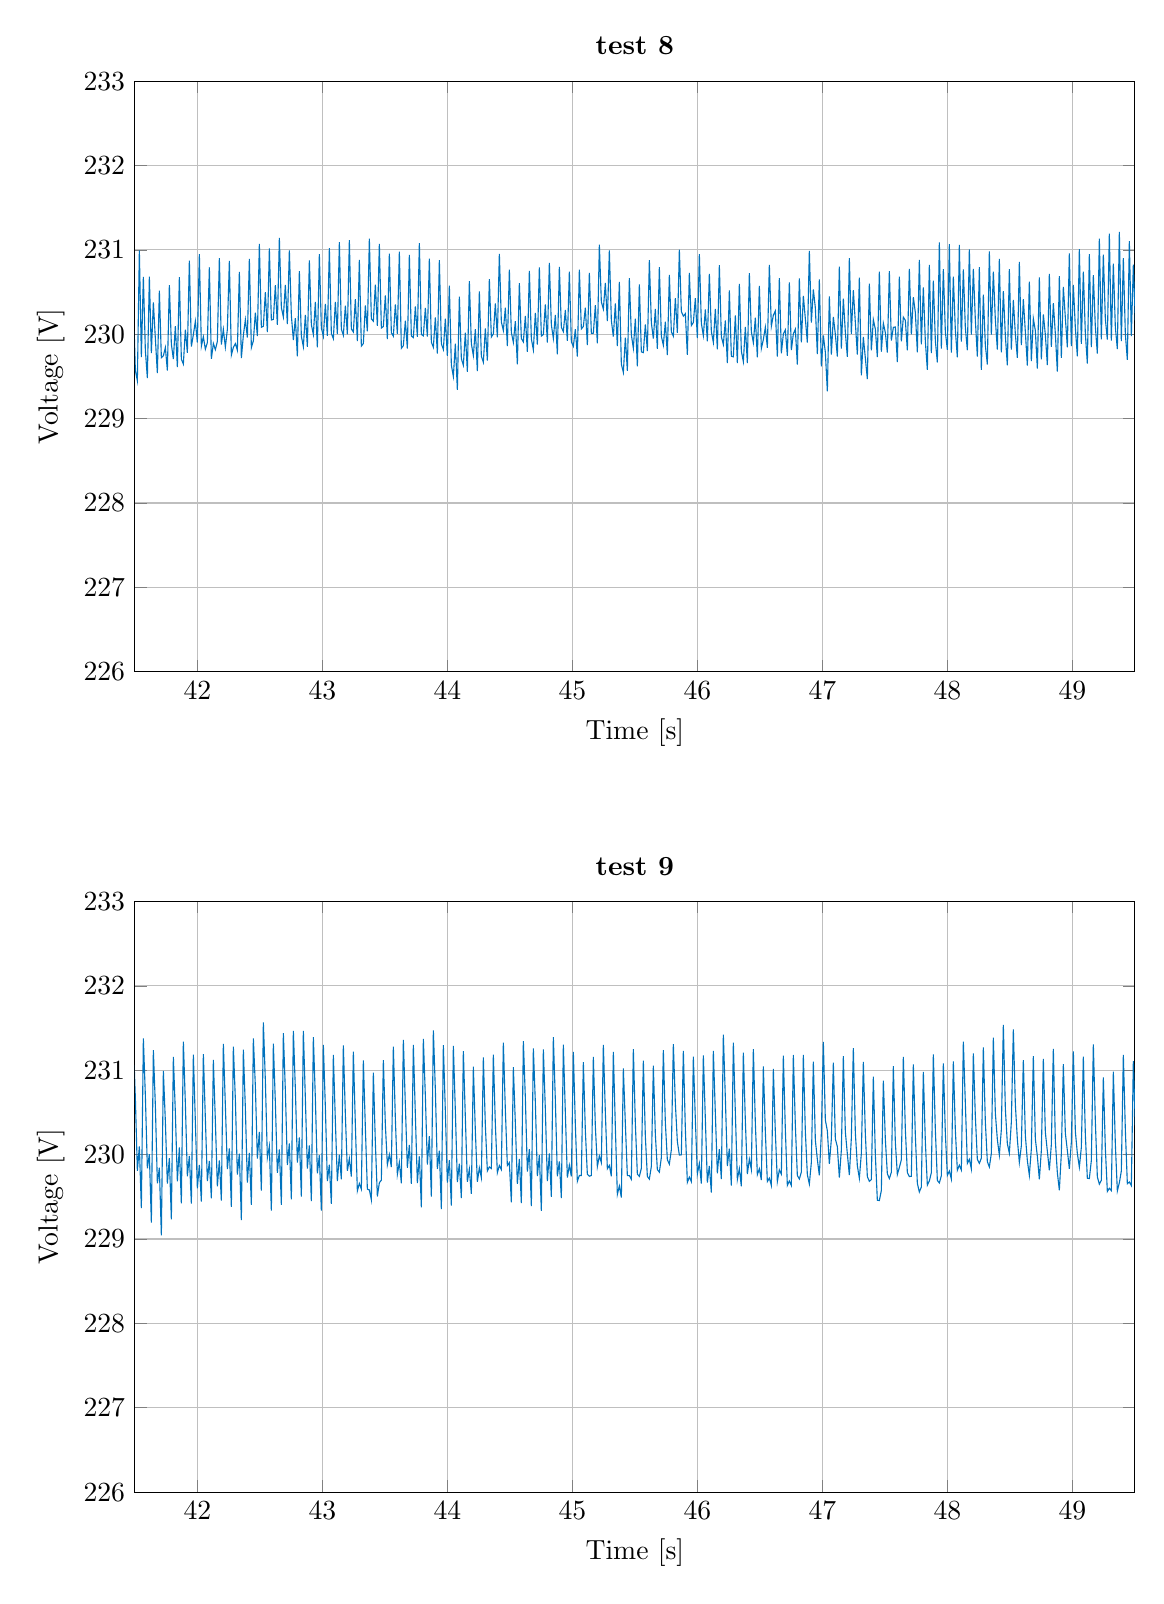
\begin{tikzpicture}

\begin{axis}[%
width=5in,
height=2.953in,
at={(1.142in,5.054in)},
scale only axis,
xmin=41.5,
xmax=49.5,
xlabel={Time [s]},
xmajorgrids,
ymin=226,
ymax=233,
ylabel={Voltage [V]},
ymajorgrids,
axis background/.style={fill=white},
title style={font=\bfseries},
title={test 8}
]
\addplot [color=mycolor1,solid,forget plot]
  table[row sep=crcr]{%
41.488	230.372353530648\\
41.504	229.57082589941\\
41.52	229.450031842589\\
41.536	230.992507802526\\
41.552	229.728135735208\\
41.568	230.680071665386\\
41.584	229.808742431885\\
41.6	229.481185974456\\
41.616	230.683176108015\\
41.632	229.776887479283\\
41.648	230.377988366188\\
41.664	229.949136633382\\
41.68	229.538143098871\\
41.696	230.515476007127\\
41.712	229.722096121419\\
41.728	229.743854409472\\
41.744	229.842070558922\\
41.76	229.569977799717\\
41.776	230.580894916615\\
41.792	229.882361673683\\
41.808	229.705823301768\\
41.824	230.096546979126\\
41.84	229.609340151519\\
41.856	230.676442997835\\
41.872	229.704401024046\\
41.888	229.647048799177\\
41.904	230.053889011409\\
41.92	229.780108104251\\
41.936	230.87219186443\\
41.952	229.85321463451\\
41.968	229.994507238923\\
41.984	230.153481093022\\
42	229.902072460373\\
42.016	230.950176514592\\
42.032	229.857294790684\\
42.048	229.969607424457\\
42.064	229.822524975388\\
42.08	229.900858393728\\
42.096	230.793576168335\\
42.112	229.707585385976\\
42.128	229.889868297599\\
42.144	229.817159821739\\
42.16	229.913663481962\\
42.176	230.901801716387\\
42.192	229.878122964753\\
42.208	230.057795538475\\
42.224	229.846409929028\\
42.24	230.056527835258\\
42.256	230.868996986354\\
42.272	229.752694692572\\
42.288	229.843738763543\\
42.304	229.887960583974\\
42.32	229.811367251382\\
42.336	230.739337163475\\
42.352	229.716234091412\\
42.368	229.98479013125\\
42.384	230.172405573965\\
42.4	229.961369708567\\
42.416	230.892717029205\\
42.432	229.840822133191\\
42.448	229.920944330145\\
42.464	230.255961366124\\
42.48	229.978071735042\\
42.496	231.070184973428\\
42.512	230.083005885533\\
42.528	230.094402442603\\
42.544	230.499105920214\\
42.56	230.025540059084\\
42.576	231.015828394836\\
42.592	230.168587627074\\
42.608	230.175829985308\\
42.624	230.581729643294\\
42.64	230.110195235147\\
42.656	231.142424813531\\
42.672	230.315903269201\\
42.688	230.205354602101\\
42.704	230.584942725863\\
42.72	230.11997745197\\
42.736	230.993983899969\\
42.752	230.222780324098\\
42.768	229.93188976717\\
42.784	230.191471882111\\
42.8	229.736809339101\\
42.816	230.748687278125\\
42.832	229.976251075503\\
42.848	229.852643580553\\
42.864	230.230123165196\\
42.88	229.850326503323\\
42.896	230.874081245495\\
42.912	230.112790717253\\
42.928	229.997113699432\\
42.944	230.382105496403\\
42.96	229.843650828059\\
42.976	230.948657242364\\
42.992	230.074390604351\\
43.008	229.975074395859\\
43.024	230.359043301586\\
43.04	229.979824446672\\
43.056	231.020390021413\\
43.072	230.008880485803\\
43.088	229.94785111975\\
43.104	230.383529993506\\
43.12	230.001317844534\\
43.136	231.092148888229\\
43.152	230.060422773141\\
43.168	229.987359241053\\
43.184	230.337716570468\\
43.2	229.9992108496\\
43.216	231.114988418558\\
43.232	230.062253339032\\
43.248	230.027120760196\\
43.264	230.414577135058\\
43.28	229.919126729395\\
43.296	230.882137370938\\
43.312	229.859553014492\\
43.328	229.889647806143\\
43.344	230.341836180569\\
43.36	230.032820798761\\
43.376	231.13201472607\\
43.392	230.181544826889\\
43.408	230.154461895653\\
43.424	230.588521331336\\
43.44	230.098387874525\\
43.456	231.069919982177\\
43.472	230.073471470561\\
43.488	230.091800683482\\
43.504	230.460610375018\\
43.52	229.942314102944\\
43.536	230.953939180858\\
43.552	230.017214195462\\
43.568	229.976936014738\\
43.584	230.353485927\\
43.6	230.005047563651\\
43.616	230.978472396485\\
43.632	229.832720940359\\
43.648	229.864066158204\\
43.664	230.160548831388\\
43.68	229.829527956829\\
43.696	230.940427741294\\
43.712	229.979045025618\\
43.728	229.960209834216\\
43.744	230.329611854063\\
43.76	229.970104691418\\
43.776	231.079580268709\\
43.792	229.997714461698\\
43.808	229.98090086181\\
43.824	230.312352408114\\
43.84	229.972639645895\\
43.856	230.894485098095\\
43.872	229.906247442798\\
43.888	229.845753973681\\
43.904	230.199322683262\\
43.92	229.769157589812\\
43.936	230.878409089282\\
43.952	229.886472218986\\
43.968	229.819991858692\\
43.984	230.185198622521\\
44	229.742823658623\\
44.016	230.575677322795\\
44.032	229.634507030898\\
44.048	229.498784035022\\
44.064	229.887256056659\\
44.08	229.340487898633\\
44.096	230.445040131317\\
44.112	229.709873743866\\
44.128	229.633331138472\\
44.144	230.01983081796\\
44.16	229.555125469314\\
44.176	230.627731311927\\
44.192	229.887122410291\\
44.208	229.747321957822\\
44.224	230.059827091354\\
44.24	229.56271035951\\
44.256	230.50624092611\\
44.272	229.738662005017\\
44.288	229.66833299835\\
44.304	230.069060040371\\
44.32	229.686011570365\\
44.336	230.653585009976\\
44.352	229.967134222061\\
44.368	230.003649754338\\
44.384	230.363753361439\\
44.4	229.963967563951\\
44.416	230.952227945522\\
44.432	230.145170933203\\
44.448	230.043976963823\\
44.464	230.314252758158\\
44.48	229.86033527016\\
44.496	230.764341719609\\
44.512	230.021161389273\\
44.528	229.903555749489\\
44.544	230.15521744089\\
44.56	229.641493949253\\
44.576	230.604013598247\\
44.592	229.94932407267\\
44.608	229.909415915047\\
44.624	230.216191467933\\
44.64	229.79004826639\\
44.656	230.750822207022\\
44.672	229.945453096357\\
44.688	229.815044586299\\
44.704	230.254027614021\\
44.72	229.87572530586\\
44.736	230.793262856627\\
44.752	229.977634793442\\
44.768	229.99707657745\\
44.784	230.353502286233\\
44.8	229.899290896253\\
44.816	230.846315230852\\
44.832	230.110979685952\\
44.848	229.949766564235\\
44.864	230.228152247245\\
44.88	229.760491078498\\
44.896	230.798761338959\\
44.912	230.081985470875\\
44.928	230.030980938037\\
44.944	230.287263598555\\
44.96	229.921593416485\\
44.976	230.741805963142\\
44.992	229.909832305128\\
45.008	229.856484202687\\
45.024	230.059572376582\\
45.04	229.735915564045\\
45.056	230.766456527371\\
45.072	230.063187463867\\
45.088	230.091359139027\\
45.104	230.314078369002\\
45.12	229.870589333917\\
45.136	230.72734561205\\
45.152	230.009570015938\\
45.168	230.012255375849\\
45.184	230.343468817283\\
45.2	229.891158044794\\
45.216	231.06087167846\\
45.232	230.381950997674\\
45.248	230.298836811761\\
45.264	230.607297527501\\
45.28	230.154346049718\\
45.296	230.993521792836\\
45.312	230.162050480415\\
45.328	229.970783023751\\
45.344	230.364066147508\\
45.36	229.858473126026\\
45.376	230.620264688873\\
45.392	229.64492484413\\
45.408	229.547832260122\\
45.424	229.960529101533\\
45.44	229.566450905806\\
45.456	230.664585423297\\
45.472	229.993551324532\\
45.488	229.833597506243\\
45.504	230.185203084462\\
45.52	229.618496892828\\
45.536	230.589607215497\\
45.552	229.790348286529\\
45.568	229.782281133431\\
45.584	230.117163664082\\
45.6	229.800879090934\\
45.616	230.878650804185\\
45.632	230.13655368816\\
45.648	229.947267963802\\
45.664	230.299195273676\\
45.68	229.827862444618\\
45.696	230.794778538136\\
45.712	229.975396744712\\
45.728	229.870033163721\\
45.744	230.147767560936\\
45.76	229.752518965722\\
45.776	230.702938273816\\
45.792	230.027337458377\\
45.808	229.977273982872\\
45.824	230.42715644661\\
45.84	230.014820347888\\
45.856	231.003705313051\\
45.872	230.268171844687\\
45.888	230.214679183794\\
45.904	230.243266031726\\
45.92	229.756226370172\\
45.936	230.726821596184\\
45.952	230.102221373155\\
45.968	230.13820942399\\
45.984	230.427463047029\\
46	229.954021212886\\
46.016	230.950151926663\\
46.032	230.128247573704\\
46.048	229.983912752905\\
46.064	230.294619603446\\
46.08	229.915161547337\\
46.096	230.716465869953\\
46.112	230.031738573769\\
46.128	229.903623475891\\
46.144	230.301418656247\\
46.16	229.819235576538\\
46.176	230.817605340681\\
46.192	229.970219768011\\
46.208	229.878718746239\\
46.224	230.163209079242\\
46.24	229.658120643506\\
46.256	230.520137539156\\
46.272	229.739190981445\\
46.288	229.732569448263\\
46.304	230.223419739496\\
46.32	229.657950091713\\
46.336	230.595976342717\\
46.352	229.800223747754\\
46.368	229.675257532034\\
46.384	230.086976184882\\
46.4	229.657870440913\\
46.416	230.722693642231\\
46.432	230.029019532227\\
46.448	229.900165763874\\
46.464	230.196783565311\\
46.48	229.724424551654\\
46.496	230.571537654842\\
46.512	229.829936629331\\
46.528	229.936991231896\\
46.544	230.083098202304\\
46.56	229.839323471846\\
46.576	230.821071237332\\
46.592	230.094545009788\\
46.608	230.225664745784\\
46.624	230.275686523904\\
46.64	229.73347248252\\
46.656	230.663724946708\\
46.672	229.774106020158\\
46.688	230.002621857592\\
46.704	230.050828479235\\
46.72	229.744498249919\\
46.736	230.613430791425\\
46.752	229.81216585239\\
46.768	230.004260400348\\
46.784	230.059119285218\\
46.8	229.638708123303\\
46.816	230.661581884892\\
46.832	229.90218534702\\
46.848	230.455229758041\\
46.864	230.182825608229\\
46.88	229.900758575245\\
46.896	230.98891809487\\
46.912	230.136417155246\\
46.928	230.530452966682\\
46.944	230.311468634463\\
46.96	229.763981341584\\
46.976	230.650320274123\\
46.992	229.617783346099\\
47.008	229.985352291171\\
47.024	229.785497263225\\
47.04	229.321496083438\\
47.056	230.44798847309\\
47.072	229.757991357373\\
47.088	230.205464682218\\
47.104	229.999125267729\\
47.12	229.735981629284\\
47.136	230.8022186379\\
47.152	229.829414427987\\
47.168	230.422710346798\\
47.184	230.022105626264\\
47.2	229.733097865222\\
47.216	230.900471742189\\
47.232	230.005587644768\\
47.248	230.521566442276\\
47.264	230.136366741289\\
47.28	229.759011814554\\
47.296	230.671343560239\\
47.312	229.513782957285\\
47.328	229.966998310355\\
47.344	229.716608061843\\
47.36	229.466882548888\\
47.376	230.600391681619\\
47.392	229.808415850609\\
47.408	230.172200542102\\
47.424	230.059969017288\\
47.44	229.727540061203\\
47.456	230.741880604169\\
47.472	229.79257801643\\
47.488	230.130031935143\\
47.504	230.019163233253\\
47.52	229.782621373945\\
47.536	230.746939327765\\
47.552	229.925682459877\\
47.568	230.080917085394\\
47.584	230.085924891962\\
47.6	229.669951107997\\
47.616	230.681033087576\\
47.632	229.914767530653\\
47.648	230.201965635721\\
47.664	230.16373129471\\
47.68	229.809115755521\\
47.696	230.775683421315\\
47.712	229.998957426175\\
47.728	230.438455442866\\
47.744	230.25766841188\\
47.76	229.786249644888\\
47.776	230.880530752959\\
47.792	229.880552175476\\
47.808	230.555555063471\\
47.824	229.91681184069\\
47.84	229.577149866126\\
47.856	230.822545528803\\
47.872	229.775028968712\\
47.888	230.6350513216\\
47.904	229.924483224404\\
47.92	229.665197675109\\
47.936	231.089672846344\\
47.952	229.828737482031\\
47.968	230.770877797064\\
47.984	230.030118176258\\
48	229.815307817602\\
48.016	231.067252499162\\
48.032	229.780617492717\\
48.048	230.682774568129\\
48.064	230.048765198654\\
48.08	229.725092614335\\
48.096	231.058365395655\\
48.112	229.911014332743\\
48.128	230.767311170501\\
48.144	230.078243576981\\
48.16	229.810345324355\\
48.176	231.005409426188\\
48.192	229.995347971789\\
48.208	230.77364993169\\
48.224	230.169930950947\\
48.24	229.735056008584\\
48.256	230.794933843362\\
48.272	229.577347284998\\
48.288	230.468136483353\\
48.304	229.870290039947\\
48.32	229.64132251192\\
48.336	230.982560822118\\
48.352	229.995725878992\\
48.368	230.742301578319\\
48.384	230.173135291038\\
48.4	229.817056048996\\
48.416	230.891674384806\\
48.432	229.784728733911\\
48.448	230.511679724661\\
48.464	229.983676827447\\
48.48	229.630512617758\\
48.496	230.772711159444\\
48.512	229.816785040375\\
48.528	230.405722628894\\
48.544	230.003589227215\\
48.56	229.719570782156\\
48.576	230.856489881839\\
48.592	229.872313945636\\
48.608	230.415339027888\\
48.624	230.027743392923\\
48.64	229.629024038951\\
48.656	230.624679777612\\
48.672	229.68241593067\\
48.688	230.185791269979\\
48.704	230.041756918633\\
48.72	229.593701132725\\
48.736	230.672411629639\\
48.752	229.702901776166\\
48.768	230.235495592046\\
48.784	229.993707354641\\
48.8	229.633162012863\\
48.816	230.715131044806\\
48.832	229.85119022964\\
48.848	230.367010983472\\
48.864	230.006873168933\\
48.88	229.557109347157\\
48.896	230.689796918461\\
48.912	229.720499601088\\
48.928	230.560557106916\\
48.944	230.195070095891\\
48.96	229.844325399419\\
48.976	230.959092208104\\
48.992	229.859080749253\\
49.008	230.585558365131\\
49.024	230.078885233555\\
49.04	229.738093072123\\
49.056	231.007668111241\\
49.072	229.884630063767\\
49.088	230.742059906686\\
49.104	230.008573446796\\
49.12	229.651658883466\\
49.136	230.949309178815\\
49.152	229.84673573891\\
49.168	230.699501842223\\
49.184	230.089001657866\\
49.2	229.77038568383\\
49.216	231.133876054976\\
49.232	229.938969095659\\
49.248	230.944622047232\\
49.264	230.181719806721\\
49.28	229.936404543554\\
49.296	231.192875987946\\
49.312	229.925384281411\\
49.328	230.8353409836\\
49.344	230.083143762957\\
49.36	229.823462151707\\
49.376	231.211633386152\\
49.392	229.916941210823\\
49.408	230.901838942736\\
49.424	230.004954624926\\
49.44	229.695090316981\\
49.456	231.103371149277\\
49.472	229.978739469858\\
49.488	230.824822250392\\
49.504	230.154135160992\\
};
\end{axis}

\begin{axis}[%
width=5in,
height=2.953in,
at={(1.142in,0.952in)},
scale only axis,
xmin=41.5,
xmax=49.5,
xlabel={Time [s]},
xmajorgrids,
ymin=226,
ymax=233,
ylabel={Voltage [V]},
ymajorgrids,
axis background/.style={fill=white},
title style={font=\bfseries},
title={test 9}
]
\addplot [color=mycolor1,solid,forget plot]
  table[row sep=crcr]{%
41.488	231.341376565234\\
41.504	230.671123915275\\
41.52	229.808541265572\\
41.536	230.098640333025\\
41.552	229.364724857439\\
41.568	231.377207373361\\
41.584	230.699089706268\\
41.6	229.837639015292\\
41.616	230.004937935723\\
41.632	229.193571502076\\
41.648	231.237378589283\\
41.664	230.584263449081\\
41.68	229.659356572836\\
41.696	229.844581265617\\
41.712	229.04320922876\\
41.728	230.993287781312\\
41.744	230.39435493446\\
41.76	229.655882659834\\
41.776	229.959054676007\\
41.792	229.231414022103\\
41.808	231.158622555522\\
41.824	230.499194874078\\
41.84	229.682359577353\\
41.856	230.085071713224\\
41.872	229.421398543759\\
41.888	231.340324510374\\
41.904	230.605492187263\\
41.92	229.743859247759\\
41.936	229.984468303713\\
41.952	229.420753398883\\
41.968	231.185402985753\\
41.984	230.389951302691\\
42	229.600889018637\\
42.016	229.879325250644\\
42.032	229.443489268788\\
42.048	231.192256767046\\
42.064	230.428312805975\\
42.08	229.685938983756\\
42.096	229.925865056738\\
42.112	229.480399066333\\
42.128	231.1221357585\\
42.144	230.40200002171\\
42.16	229.623726825713\\
42.176	229.930750437286\\
42.192	229.455963319421\\
42.208	231.31320888258\\
42.224	230.584872315875\\
42.24	229.829814999952\\
42.256	230.073384823053\\
42.272	229.380255687285\\
42.288	231.280088464537\\
42.304	230.657810184497\\
42.32	229.762852495237\\
42.336	230.012376131155\\
42.352	229.224144715799\\
42.368	231.243564515944\\
42.384	230.554642112384\\
42.4	229.66929952843\\
42.416	230.020640835503\\
42.432	229.403892494198\\
42.448	231.377177283976\\
42.464	230.813823960264\\
42.48	229.95334090182\\
42.496	230.269841252693\\
42.512	229.572195890233\\
42.528	231.568623953949\\
42.544	230.877653453612\\
42.56	229.962930447568\\
42.576	230.097204780689\\
42.592	229.334983257921\\
42.608	231.315027203539\\
42.624	230.617926357698\\
42.64	229.783768223265\\
42.656	230.060758462117\\
42.672	229.405901012751\\
42.688	231.439522838304\\
42.704	230.759603418238\\
42.72	229.87743526236\\
42.736	230.132217335598\\
42.752	229.470960668736\\
42.768	231.467710289987\\
42.784	230.780971902695\\
42.8	229.906848569524\\
42.816	230.203962803497\\
42.832	229.501759861028\\
42.848	231.467830370163\\
42.864	230.66867151962\\
42.88	229.833679275843\\
42.896	230.109538327353\\
42.912	229.450355527593\\
42.928	231.393251417504\\
42.944	230.671610582368\\
42.96	229.777829339561\\
42.976	229.992193970566\\
42.992	229.336612692407\\
43.008	231.300461590524\\
43.024	230.567032239426\\
43.04	229.685249119727\\
43.056	229.881594604692\\
43.072	229.415377508078\\
43.088	231.182318622245\\
43.104	230.401764118826\\
43.12	229.686911872206\\
43.136	229.999519114813\\
43.152	229.707020193307\\
43.168	231.295910504518\\
43.184	230.474279746075\\
43.2	229.807030472537\\
43.216	229.95263042875\\
43.232	229.740745662581\\
43.248	231.219312853128\\
43.264	230.355438170671\\
43.28	229.570720854631\\
43.296	229.657800279037\\
43.312	229.592298625555\\
43.328	231.117674961046\\
43.344	230.319728076575\\
43.36	229.590879505157\\
43.376	229.581507643899\\
43.392	229.465352904786\\
43.408	230.973138958687\\
43.424	230.143968114317\\
43.44	229.504284433604\\
43.456	229.666754894778\\
43.472	229.697658310053\\
43.488	231.119136984529\\
43.504	230.356282439312\\
43.52	229.880633544049\\
43.536	230.000422112438\\
43.552	229.852637537193\\
43.568	231.279057680602\\
43.584	230.424805292929\\
43.6	229.766445027663\\
43.616	229.907911977388\\
43.632	229.660758763409\\
43.648	231.358768074425\\
43.664	230.583492637566\\
43.68	229.844730879584\\
43.696	230.115289911502\\
43.712	229.65230540762\\
43.728	231.300104843308\\
43.744	230.472576249518\\
43.76	229.663389271253\\
43.776	229.980261003731\\
43.792	229.375918819422\\
43.808	231.372339387295\\
43.824	230.696051419057\\
43.84	229.883194215513\\
43.856	230.220127525074\\
43.872	229.501598790868\\
43.888	231.473012895951\\
43.904	230.770224657807\\
43.92	229.830132765688\\
43.936	230.045834772845\\
43.952	229.355401153743\\
43.968	231.29895746026\\
43.984	230.509167807374\\
44	229.669323101562\\
44.016	229.933997627602\\
44.032	229.396693239728\\
44.048	231.288474701991\\
44.064	230.516598196837\\
44.08	229.674504814807\\
44.096	229.892873771094\\
44.112	229.483325594258\\
44.128	231.227437747583\\
44.144	230.437111985691\\
44.16	229.677867053416\\
44.176	229.8274500724\\
44.192	229.534147825747\\
44.208	231.042380141281\\
44.224	230.279409209526\\
44.24	229.677677763906\\
44.256	229.842666394718\\
44.272	229.72828311165\\
44.288	231.151359803793\\
44.304	230.346880805329\\
44.32	229.807157817432\\
44.336	229.853743422696\\
44.352	229.835854740287\\
44.368	231.184893260491\\
44.384	230.359428245934\\
44.4	229.785520552677\\
44.416	229.870646196247\\
44.432	229.823766279047\\
44.448	231.327811356131\\
44.464	230.527845146075\\
44.48	229.871380465745\\
44.496	229.904781535191\\
44.512	229.434717200527\\
44.528	231.037593493784\\
44.544	230.370267304342\\
44.56	229.652608862203\\
44.576	229.947938976963\\
44.592	229.424692948988\\
44.608	231.344965723726\\
44.624	230.67142892741\\
44.64	229.798778597147\\
44.656	230.063587910346\\
44.672	229.389887509403\\
44.688	231.257749845537\\
44.704	230.617181034452\\
44.72	229.744467607969\\
44.736	229.992432582728\\
44.752	229.334448888668\\
44.768	231.247630799153\\
44.784	230.534021167465\\
44.8	229.685922261602\\
44.816	230.013150477779\\
44.832	229.500483299036\\
44.848	231.391874207438\\
44.864	230.643145892368\\
44.88	229.74237848616\\
44.896	229.918407729293\\
44.912	229.484697476294\\
44.928	231.30235938694\\
44.944	230.491620301955\\
44.96	229.727646960017\\
44.976	229.874572714674\\
44.992	229.741451886426\\
45.008	231.216632016648\\
45.024	230.352088984921\\
45.04	229.684206656963\\
45.056	229.752759307634\\
45.072	229.751820168585\\
45.088	231.097597233917\\
45.104	230.285574172067\\
45.12	229.766299488952\\
45.136	229.744478427283\\
45.152	229.752804469878\\
45.168	231.158125418947\\
45.184	230.332720198355\\
45.2	229.858123865896\\
45.216	229.983459258705\\
45.232	229.90574174901\\
45.248	231.301111977009\\
45.264	230.494889510815\\
45.28	229.831883163119\\
45.296	229.871653056379\\
45.312	229.743723707181\\
45.328	231.217207355275\\
45.344	230.325413057522\\
45.36	229.528142865617\\
45.376	229.628022207283\\
45.392	229.492037133033\\
45.408	231.022782381114\\
45.424	230.367081085998\\
45.44	229.751452766997\\
45.456	229.751932545591\\
45.472	229.708002211463\\
45.488	231.249261209425\\
45.504	230.366517135308\\
45.52	229.769083407331\\
45.536	229.742356349094\\
45.552	229.837325317988\\
45.568	231.114409034125\\
45.584	230.215467395263\\
45.6	229.742115602679\\
45.616	229.709665536279\\
45.632	229.860268428182\\
45.648	231.054163228651\\
45.664	230.239440323535\\
45.68	229.822643245618\\
45.696	229.792310865044\\
45.712	229.964814370046\\
45.728	231.237757612624\\
45.744	230.379176148365\\
45.76	229.938718953286\\
45.776	229.886860844924\\
45.792	230.05795868417\\
45.808	231.308620991573\\
45.824	230.609597585424\\
45.84	230.154515589108\\
45.856	229.995127160696\\
45.872	229.996991383228\\
45.888	231.229567895069\\
45.904	230.307396711471\\
45.92	229.670810870902\\
45.936	229.733890332249\\
45.952	229.680157491403\\
45.968	231.161082763619\\
45.984	230.413090556682\\
46	229.770534488995\\
46.016	229.894901422876\\
46.032	229.657165259462\\
46.048	231.17533464007\\
46.064	230.420474176535\\
46.08	229.668970044793\\
46.096	229.8671443299\\
46.112	229.550162117826\\
46.128	231.228874953491\\
46.144	230.488522026539\\
46.16	229.779148081169\\
46.176	230.064931337213\\
46.192	229.710632265817\\
46.208	231.422487198167\\
46.224	230.672343059238\\
46.24	229.863992174434\\
46.256	230.071398643616\\
46.272	229.633749844579\\
46.288	231.325970894373\\
46.304	230.498449798269\\
46.32	229.705181403444\\
46.336	229.832115913817\\
46.352	229.623453598402\\
46.368	231.20869551465\\
46.384	230.400442566132\\
46.4	229.769410138337\\
46.416	229.945280835721\\
46.432	229.824674755406\\
46.448	231.250333211711\\
46.464	230.372107680024\\
46.48	229.762946388495\\
46.496	229.832127562403\\
46.512	229.697601182139\\
46.528	231.046607673545\\
46.544	230.269376048632\\
46.56	229.681154275566\\
46.576	229.721148722693\\
46.592	229.635014452312\\
46.608	231.017475498247\\
46.624	230.264580713156\\
46.64	229.681504358603\\
46.656	229.818221276342\\
46.672	229.768714737948\\
46.688	231.17278495842\\
46.704	230.293183608863\\
46.72	229.63494832326\\
46.736	229.687351952003\\
46.752	229.635213024589\\
46.768	231.180608595965\\
46.784	230.346349862285\\
46.8	229.752510787857\\
46.816	229.711268786752\\
46.832	229.792544474199\\
46.848	231.180721972073\\
46.864	230.273115522412\\
46.88	229.762604955899\\
46.896	229.651718733446\\
46.912	229.907738835072\\
46.928	231.103358714475\\
46.944	230.171141876489\\
46.96	229.944147232329\\
46.976	229.753365494186\\
46.992	230.252607777836\\
47.008	231.33633168369\\
47.024	230.408949279473\\
47.04	230.282567010233\\
47.056	229.889721980912\\
47.072	230.181933714204\\
47.088	231.089671599515\\
47.104	230.18532124279\\
47.12	230.094794574586\\
47.136	229.726915167122\\
47.152	230.052178651563\\
47.168	231.166043599012\\
47.184	230.269492744235\\
47.2	230.009380137135\\
47.216	229.756510829615\\
47.232	230.197285092649\\
47.248	231.262127581768\\
47.264	230.258309462739\\
47.28	229.867468818473\\
47.296	229.72012434315\\
47.312	230.013708853951\\
47.328	231.098620211555\\
47.344	230.243291787725\\
47.36	229.738978292876\\
47.376	229.683519779795\\
47.392	229.705005817106\\
47.408	230.923763823327\\
47.424	229.997109306139\\
47.44	229.459248459824\\
47.456	229.455487496521\\
47.472	229.574630965036\\
47.488	230.875814743976\\
47.504	230.178503873838\\
47.52	229.773145538732\\
47.536	229.716404665372\\
47.552	229.789835922544\\
47.568	231.048582390818\\
47.584	230.145080860725\\
47.6	229.764504079246\\
47.616	229.84701817062\\
47.632	229.939757735779\\
47.648	231.159430460025\\
47.664	230.297979433567\\
47.68	229.788633654572\\
47.696	229.739997467318\\
47.712	229.743462759787\\
47.728	231.069517884546\\
47.744	230.223693547706\\
47.76	229.659857248511\\
47.776	229.55729937138\\
47.792	229.61582865118\\
47.808	230.981939748358\\
47.824	230.154495950839\\
47.84	229.638973871138\\
47.856	229.687217787036\\
47.872	229.786411766307\\
47.888	231.187111578321\\
47.904	230.293815188301\\
47.92	229.69414519034\\
47.936	229.664158150214\\
47.952	229.750161639969\\
47.968	231.082367914876\\
47.984	230.252433511972\\
48	229.75358771354\\
48.016	229.804768105139\\
48.032	229.711919509658\\
48.048	231.103689223978\\
48.064	230.288015948035\\
48.08	229.815333162698\\
48.096	229.87509596984\\
48.112	229.817862040231\\
48.128	231.337763536666\\
48.144	230.606430744049\\
48.16	229.89583927648\\
48.176	229.94430284373\\
48.192	229.832140759935\\
48.208	231.199651850259\\
48.224	230.45358602309\\
48.24	229.944355532081\\
48.256	229.896935412339\\
48.272	229.957570151574\\
48.288	231.27236063462\\
48.304	230.388068928536\\
48.32	229.917042357585\\
48.336	229.853847059202\\
48.352	230.013659003037\\
48.368	231.3865855288\\
48.384	230.491489202713\\
48.4	230.17901145774\\
48.416	229.994920093848\\
48.432	230.296333266136\\
48.448	231.538763669581\\
48.464	230.545606779654\\
48.48	230.1305287566\\
48.496	230.017096066992\\
48.512	230.385325427358\\
48.528	231.483708286687\\
48.544	230.597841589913\\
48.56	230.181962288399\\
48.576	229.907329349227\\
48.592	230.104383851983\\
48.608	231.120790363171\\
48.624	230.227424880799\\
48.64	229.930032799707\\
48.656	229.755538846926\\
48.672	230.067480939258\\
48.688	231.168097193811\\
48.704	230.18669572532\\
48.72	229.981339318734\\
48.736	229.707254484467\\
48.752	230.04750175698\\
48.768	231.135742643657\\
48.784	230.266095459438\\
48.8	230.041735292656\\
48.816	229.813579059499\\
48.832	230.118125276732\\
48.848	231.252131164685\\
48.864	230.163189874206\\
48.88	229.785882336917\\
48.896	229.577744130671\\
48.912	230.013272943532\\
48.928	231.073494548259\\
48.944	230.254164459173\\
48.96	230.050059173664\\
48.976	229.830661827466\\
48.992	230.146109341895\\
49.008	231.224934710477\\
49.024	230.277058323113\\
49.04	230.014899479294\\
49.056	229.851157325496\\
49.072	230.085726498801\\
49.088	231.160340043925\\
49.104	230.237600564905\\
49.12	229.719698058448\\
49.136	229.716391776194\\
49.152	229.931102306987\\
49.168	231.306025241757\\
49.184	230.393821269727\\
49.2	229.736003802963\\
49.216	229.650483004049\\
49.232	229.695329286744\\
49.248	230.915645434617\\
49.264	230.075414414761\\
49.28	229.563240964179\\
49.296	229.600972478403\\
49.312	229.573138829042\\
49.328	230.983064754057\\
49.344	230.124875652555\\
49.36	229.570599459232\\
49.376	229.666050208693\\
49.392	229.807020401177\\
49.408	231.181253192686\\
49.424	230.29381342878\\
49.44	229.655271068954\\
49.456	229.675280946778\\
49.472	229.633275955053\\
49.488	231.109237128952\\
49.504	230.335402033574\\
};
\end{axis}
\end{tikzpicture}%
\caption{Steady state Voltage output of the genset at 50 kW load.}
\label{fig:test8-9steadyvolt50kw}
\end{figure}


%----------------------------------------------------
\subsection*{Step measurements}
\subsubsection*{Frequency}
\begin{figure}[H]
\centering
% This file was created by matlab2tikz.
%
%The latest updates can be retrieved from
%  http://www.mathworks.com/matlabcentral/fileexchange/22022-matlab2tikz-matlab2tikz
%where you can also make suggestions and rate matlab2tikz.
%
\definecolor{mycolor1}{rgb}{0.00000,0.44700,0.74100}%
%
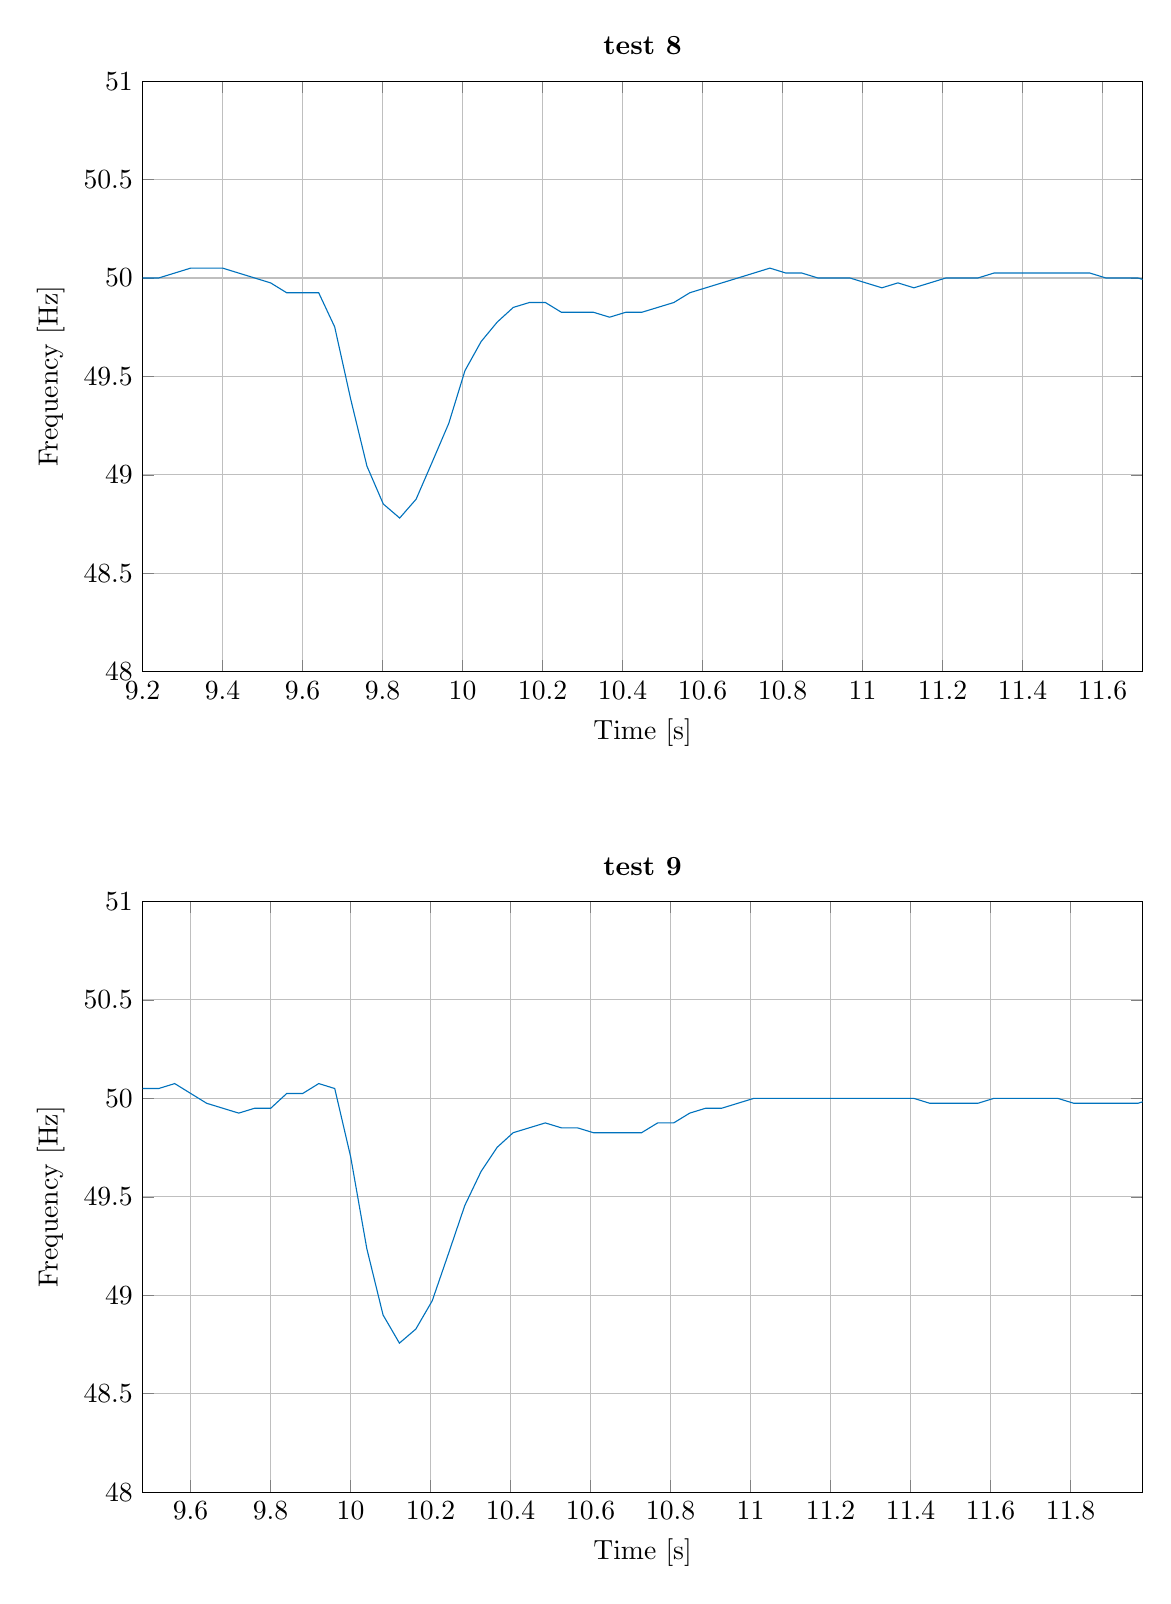
\begin{tikzpicture}

\begin{axis}[%
width=5in,
height=2.953in,
at={(1.142in,5.054in)},
scale only axis,
xmin=9.2,
xmax=11.7,
xlabel={Time [s]},
xmajorgrids,
ymin=48,
ymax=51,
ylabel={Frequency [Hz]},
ymajorgrids,
axis background/.style={fill=white},
title style={font=\bfseries},
title={test 8}
]
\addplot [color=mycolor1,solid,forget plot]
  table[row sep=crcr]{%
9.16032	49.9750124937529\\
9.20034	49.9999999999988\\
9.24034	50.0000000000011\\
9.28034	50.0250125062532\\
9.32032	50.0500500500492\\
9.36028	50.0500500500514\\
9.40024	50.0500500500492\\
9.4402	50.0250125062532\\
9.48018	49.9999999999988\\
9.52018	49.9750124937529\\
9.5602	49.9251123315044\\
9.60026	49.9251123315022\\
9.64032	49.9251123315022\\
9.68038	49.751243781094\\
9.72058	49.382716049383\\
9.76108	49.0436488474745\\
9.80186	48.8519785051305\\
9.8428	48.7804878048776\\
9.8838	48.8758553274684\\
9.92472	49.0677134445528\\
9.96548	49.2610837438429\\
10.00608	49.5294700346697\\
10.04646	49.6770988574268\\
10.08672	49.776007964162\\
10.1269	49.850448654038\\
10.16702	49.8753117206974\\
10.20712	49.8753117206996\\
10.24722	49.8256103637258\\
10.28736	49.825610363728\\
10.3275	49.8256103637258\\
10.36764	49.8007968127488\\
10.4078	49.825610363728\\
10.44794	49.825610363728\\
10.48808	49.850448654038\\
10.5282	49.8753117206974\\
10.5683	49.9251123315022\\
10.60836	49.9500499500507\\
10.6484	49.9750124937529\\
10.68842	49.9999999999988\\
10.72842	50.0250125062532\\
10.7684	50.0500500500514\\
10.80836	50.0250125062532\\
10.84834	50.0250125062532\\
10.88832	49.9999999999988\\
10.92832	50.0000000000011\\
10.96832	49.9999999999988\\
11.00832	49.9750124937529\\
11.04834	49.9500499500507\\
11.08838	49.9750124937529\\
11.1284	49.9500499500507\\
11.16844	49.9750124937529\\
11.20846	49.9999999999988\\
11.24846	50.0000000000011\\
11.28846	49.9999999999988\\
11.32846	50.0250125062532\\
11.36844	50.0250125062532\\
11.40842	50.0250125062532\\
11.4484	50.0250125062532\\
11.48838	50.0250125062532\\
11.52836	50.0250125062532\\
11.56834	50.0250125062532\\
11.60832	50.0000000000011\\
11.64832	49.9999999999988\\
11.68832	50.0000000000011\\
11.72832	49.9750124937529\\
};
\end{axis}

\begin{axis}[%
width=5in,
height=2.953in,
at={(1.142in,0.952in)},
scale only axis,
xmin=9.48,
xmax=11.98,
xlabel={Time [s]},
xmajorgrids,
ymin=48,
ymax=51,
ylabel={Frequency [Hz]},
ymajorgrids,
axis background/.style={fill=white},
title style={font=\bfseries},
title={test 9}
]
\addplot [color=mycolor1,solid,forget plot]
  table[row sep=crcr]{%
9.44052	50.0000000000011\\
9.48052	50.0500500500492\\
9.52048	50.0500500500492\\
9.56044	50.075112669004\\
9.60038	50.0250125062532\\
9.64036	49.9750124937529\\
9.68038	49.9500499500507\\
9.72042	49.9251123315022\\
9.76048	49.9500499500507\\
9.80052	49.9500499500485\\
9.84056	50.0250125062532\\
9.88054	50.0250125062532\\
9.92052	50.075112669004\\
9.96046	50.0500500500514\\
10.00042	49.7017892644126\\
10.04066	49.2368291482022\\
10.08128	48.8997555012239\\
10.12218	48.7567040468048\\
10.1632	48.8281249999999\\
10.20416	48.9715964740459\\
10.245	49.2125984251971\\
10.28564	49.4559841740848\\
10.32608	49.6277915632752\\
10.36638	49.751243781094\\
10.40658	49.825610363728\\
10.44672	49.850448654038\\
10.48684	49.8753117206974\\
10.52694	49.850448654038\\
10.56706	49.850448654038\\
10.60718	49.825610363728\\
10.64732	49.8256103637258\\
10.68746	49.825610363728\\
10.7276	49.8256103637258\\
10.76774	49.8753117206996\\
10.80784	49.8753117206974\\
10.84794	49.9251123315022\\
10.888	49.9500499500507\\
10.92804	49.9500499500507\\
10.96808	49.9750124937529\\
11.0081	49.9999999999988\\
11.0481	50.0000000000011\\
11.0881	49.9999999999988\\
11.1281	50.0000000000011\\
11.1681	50.0000000000011\\
11.2081	49.9999999999988\\
11.2481	50.0000000000011\\
11.2881	49.9999999999988\\
11.3281	50.0000000000011\\
11.3681	49.9999999999988\\
11.4081	50.0000000000011\\
11.4481	49.9750124937529\\
11.48812	49.9750124937529\\
11.52814	49.9750124937529\\
11.56816	49.9750124937529\\
11.60818	50.0000000000011\\
11.64818	49.9999999999988\\
11.68818	50.0000000000011\\
11.72818	49.9999999999988\\
11.76818	50.0000000000011\\
11.80818	49.9750124937529\\
11.8482	49.9750124937529\\
11.88822	49.9750124937529\\
11.92824	49.9750124937529\\
11.96826	49.9750124937529\\
12.00828	50.0000000000011\\
};
\end{axis}
\end{tikzpicture}%
\caption{Frequency disturbance on the output of the genset occuring from step of 10 to 20 kW load. }
\label{fig:test8-9-10to20kwstepfreq}
\end{figure}

\begin{figure}[H]
\centering
% This file was created by matlab2tikz.
%
%The latest updates can be retrieved from
%  http://www.mathworks.com/matlabcentral/fileexchange/22022-matlab2tikz-matlab2tikz
%where you can also make suggestions and rate matlab2tikz.
%
\definecolor{mycolor1}{rgb}{0.00000,0.44700,0.74100}%
%
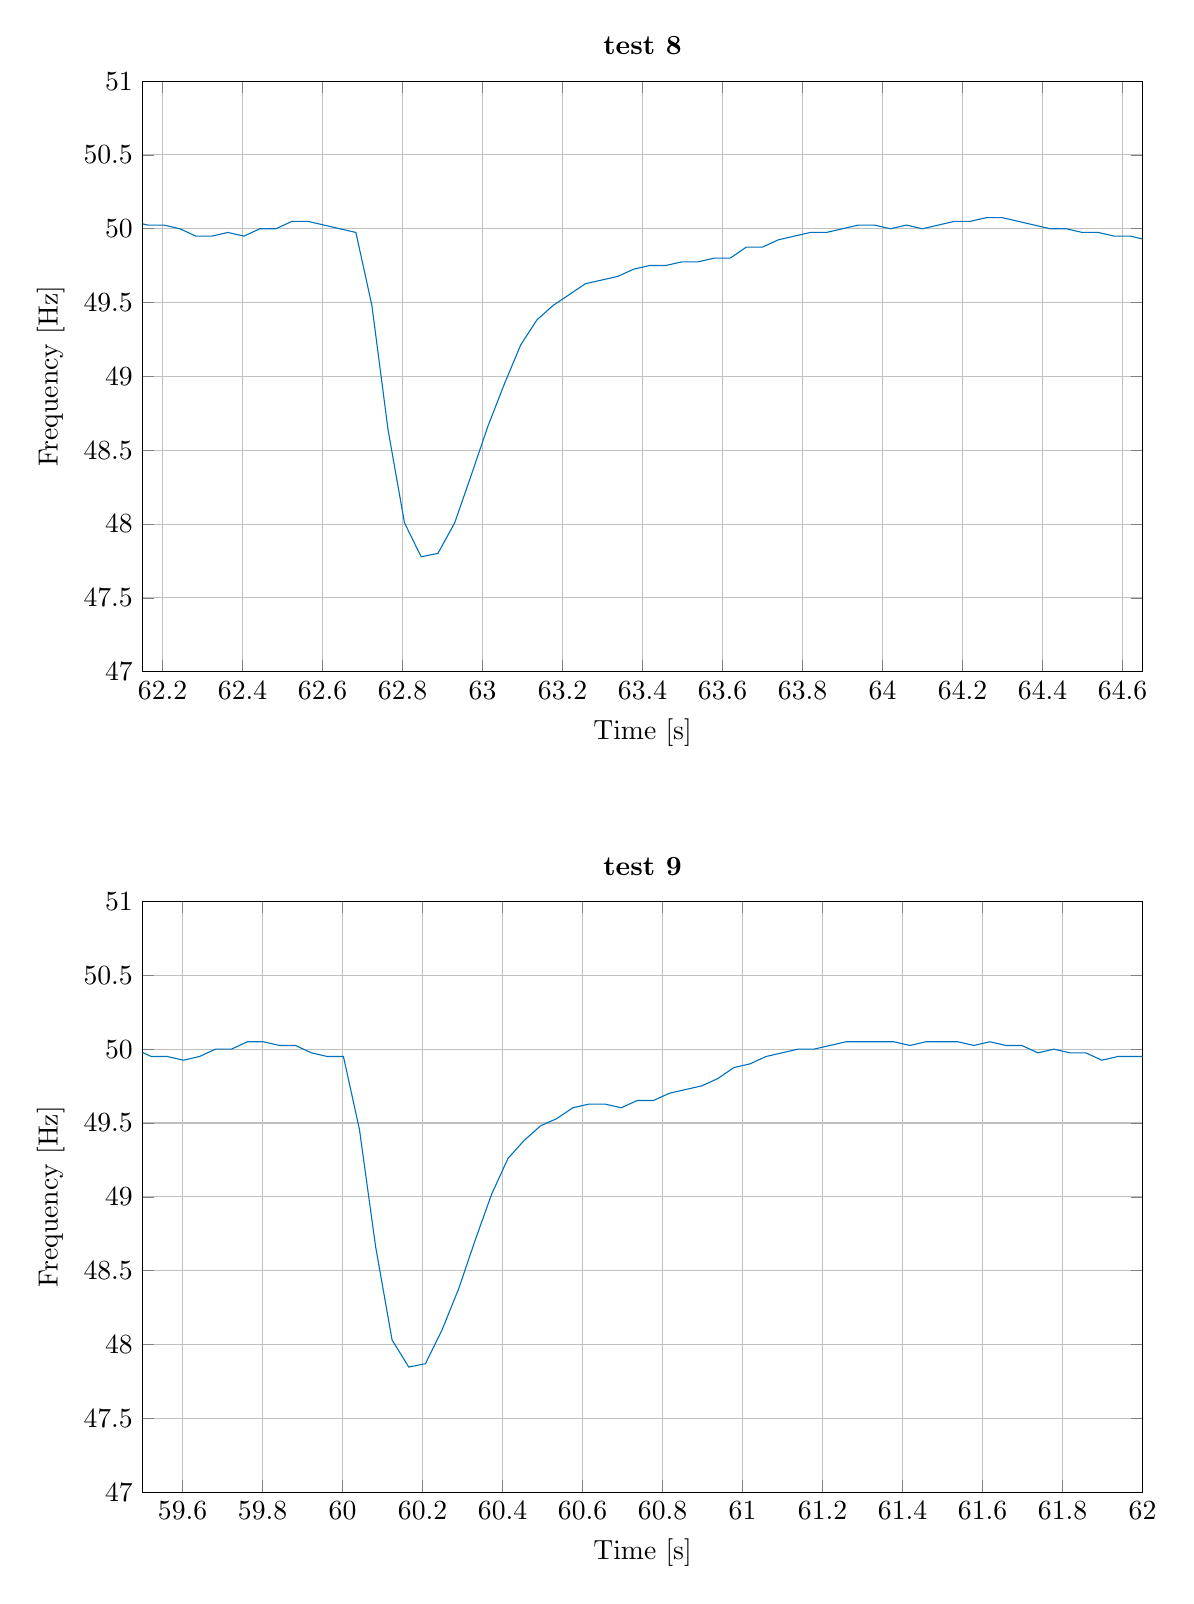
\begin{tikzpicture}

\begin{axis}[%
width=5in,
height=2.953in,
at={(1.142in,5.054in)},
scale only axis,
xmin=62.15,
xmax=64.65,
xlabel={Time [s]},
xmajorgrids,
ymin=47,
ymax=51,
ylabel={Frequency [Hz]},
ymajorgrids,
axis background/.style={fill=white},
title style={font=\bfseries},
title={test 8}
]
\addplot [color=mycolor1,solid,forget plot]
  table[row sep=crcr]{%
62.12338	50.0500500500492\\
62.16334	50.0250125062532\\
62.20332	50.0250125062532\\
62.2433	50.0000000000011\\
62.2833	49.9500499500529\\
62.32334	49.950049950044\\
62.36338	49.9750124937551\\
62.4034	49.9500499500529\\
62.44344	50.0000000000011\\
62.48344	50.0000000000011\\
62.52344	50.0500500500492\\
62.5634	50.0500500500492\\
62.60336	50.0250125062532\\
62.64334	50.0000000000011\\
62.68334	49.9750124937463\\
62.72336	49.4804552201911\\
62.76378	48.6381322957206\\
62.8049	48.0076812289963\\
62.84656	47.7783086478741\\
62.88842	47.8011472275328\\
62.93026	48.0076812289963\\
62.97192	48.3325277912074\\
63.0133	48.6618004866178\\
63.0544	48.9476260401345\\
63.09526	49.2125984251928\\
63.1359	49.3827160493895\\
63.1764	49.4804552201824\\
63.21682	49.5540138751242\\
63.25718	49.6277915632817\\
63.29748	49.6524329692121\\
63.33776	49.6770988574224\\
63.37802	49.7265042267554\\
63.41824	49.7512437810962\\
63.45844	49.7512437810962\\
63.49864	49.776007964162\\
63.53882	49.776007964162\\
63.579	49.8007968127488\\
63.61916	49.8007968127488\\
63.65932	49.8753117206952\\
63.69942	49.8753117206952\\
63.73952	49.9251123315066\\
63.77958	49.9500499500529\\
63.81962	49.9750124937463\\
63.85964	49.9750124937551\\
63.89966	50.0000000000011\\
63.93966	50.0250125062532\\
63.97964	50.0250125062532\\
64.01962	49.9999999999922\\
64.05962	50.025012506271\\
64.0996	49.9999999999922\\
64.1396	50.0250125062532\\
64.17958	50.0500500500403\\
64.21954	50.0500500500581\\
64.2595	50.0751126690017\\
64.29944	50.0751126690017\\
64.33938	50.0500500500581\\
64.37934	50.0250125062355\\
64.41932	50.0000000000099\\
64.45932	50.0000000000099\\
64.49932	49.9750124937551\\
64.53934	49.9750124937551\\
64.57936	49.950049950044\\
64.6194	49.950049950044\\
64.65944	49.9251123315066\\
};
\end{axis}

\begin{axis}[%
width=5in,
height=2.953in,
at={(1.142in,0.952in)},
scale only axis,
xmin=59.5,
xmax=62,
xlabel={Time [s]},
xmajorgrids,
ymin=47,
ymax=51,
ylabel={Frequency [Hz]},
ymajorgrids,
axis background/.style={fill=white},
title style={font=\bfseries},
title={test 9}
]
\addplot [color=mycolor1,solid,forget plot]
  table[row sep=crcr]{%
59.4821	50.0000000000011\\
59.5221	49.950049950044\\
59.56214	49.9500499500529\\
59.60218	49.9251123315066\\
59.64224	49.950049950044\\
59.68228	50.0000000000011\\
59.72228	50.0000000000011\\
59.76228	50.0500500500492\\
59.80224	50.0500500500492\\
59.8422	50.0250125062532\\
59.88218	50.0250125062532\\
59.92216	49.9750124937551\\
59.96218	49.9500499500529\\
60.00222	49.950049950044\\
60.04226	49.4559841740891\\
60.0827	48.6618004866178\\
60.1238	48.0307396733898\\
60.16544	47.8468899521508\\
60.20724	47.86979415989\\
60.24902	48.1000481000443\\
60.2906	48.3792936623147\\
60.33194	48.7092060399396\\
60.373	49.0196078431405\\
60.4138	49.2610837438365\\
60.4544	49.3827160493895\\
60.4949	49.4804552201824\\
60.53532	49.5294700346719\\
60.5757	49.6031746031731\\
60.61602	49.6277915632817\\
60.65632	49.627791563273\\
60.69662	49.6031746031731\\
60.73694	49.6524329692121\\
60.77722	49.6524329692209\\
60.8175	49.7017892644082\\
60.85774	49.7265042267554\\
60.89796	49.7512437810962\\
60.93816	49.8007968127488\\
60.97832	49.8753117206952\\
61.01842	49.9001996008032\\
61.0585	49.950049950044\\
61.09854	49.9750124937551\\
61.13856	50.0000000000011\\
61.17856	50.0000000000011\\
61.21856	50.0250125062532\\
61.25854	50.0500500500492\\
61.2985	50.0500500500492\\
61.33846	50.0500500500492\\
61.37842	50.0500500500492\\
61.41838	50.0250125062532\\
61.45836	50.0500500500492\\
61.49832	50.0500500500581\\
61.53828	50.0500500500492\\
61.57824	50.0250125062532\\
61.61822	50.0500500500492\\
61.65818	50.0250125062532\\
61.69816	50.0250125062532\\
61.73814	49.9750124937463\\
61.77816	50.0000000000011\\
61.81816	49.9750124937551\\
61.85818	49.9750124937551\\
61.8982	49.9251123314978\\
61.93826	49.9500499500529\\
61.9783	49.9500499500529\\
62.01834	49.950049950044\\
};
\end{axis}
\end{tikzpicture}%
\caption{Frequency disturbance on the output of the genset occuring from step of 10 to 30 kW load.}
\label{fig:test8-9-10to30kwstepfreq}
\end{figure}

\begin{figure}[H]
\centering
% This file was created by matlab2tikz.
%
%The latest updates can be retrieved from
%  http://www.mathworks.com/matlabcentral/fileexchange/22022-matlab2tikz-matlab2tikz
%where you can also make suggestions and rate matlab2tikz.
%
\definecolor{mycolor1}{rgb}{0.00000,0.44700,0.74100}%
%
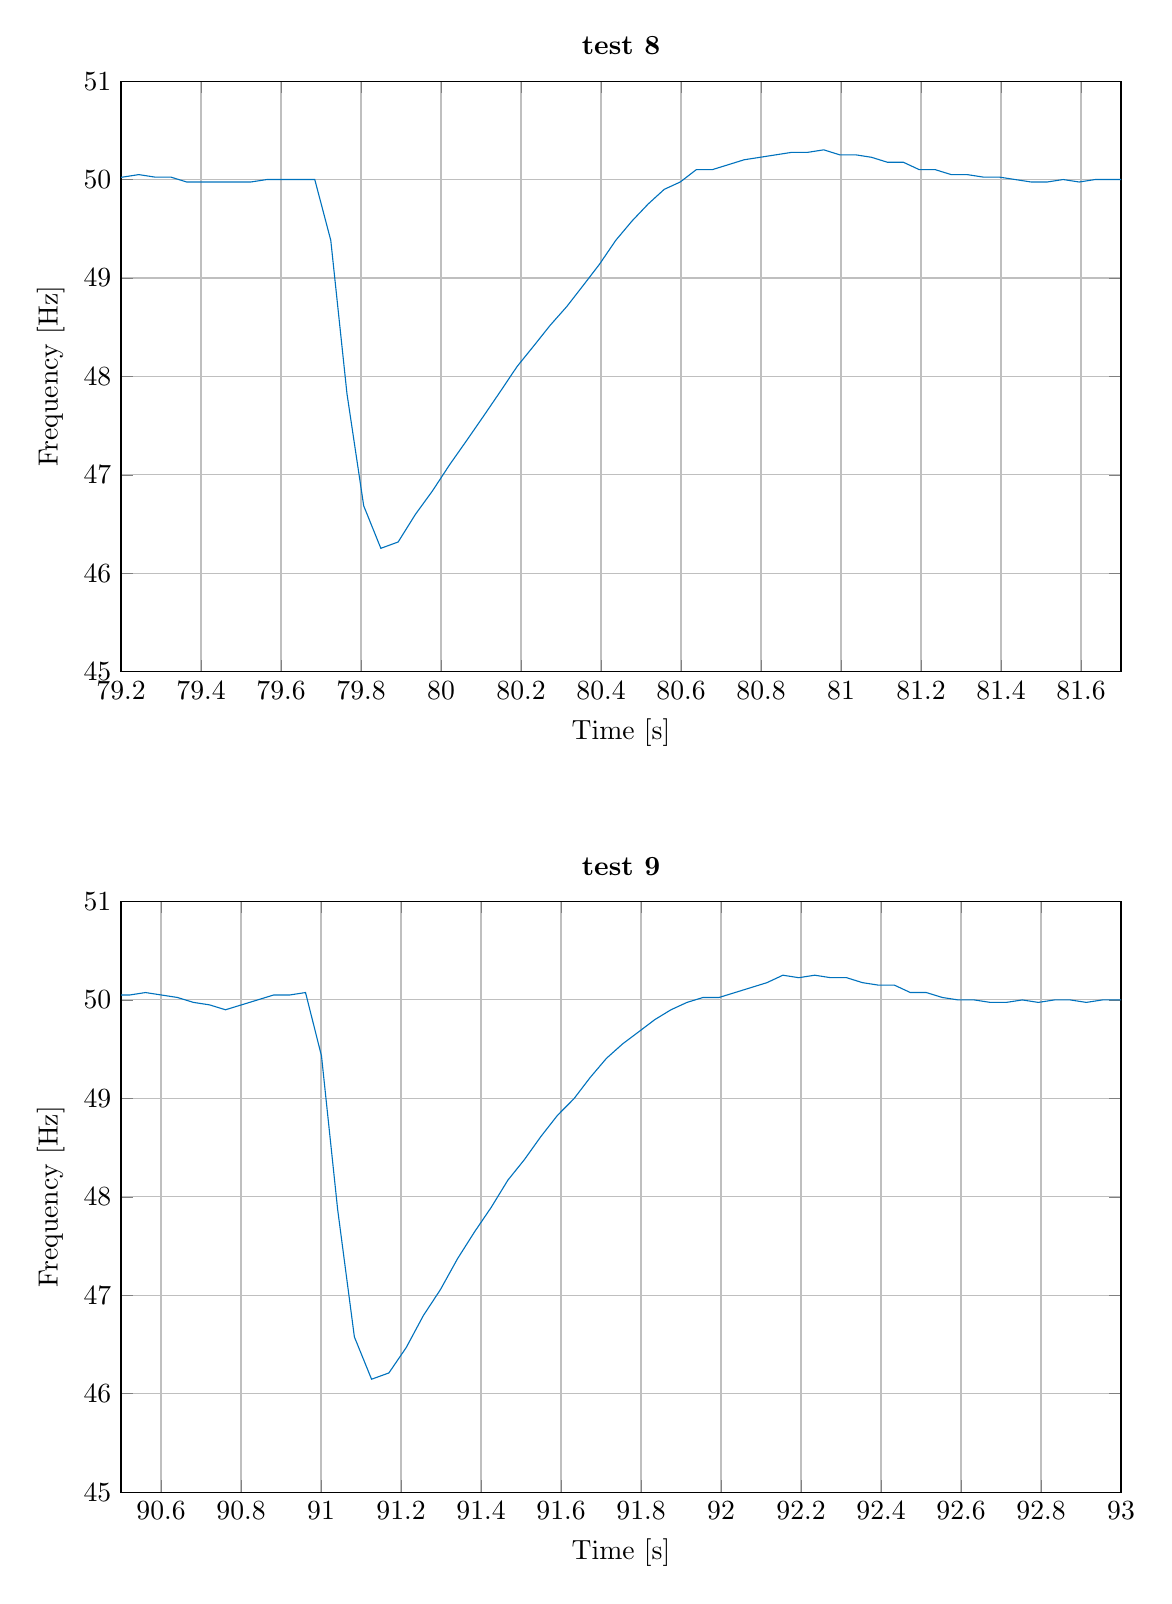
\begin{tikzpicture}

\begin{axis}[%
width=5in,
height=2.953in,
at={(1.142in,5.054in)},
scale only axis,
xmin=79.2,
xmax=81.7,
xlabel={Time [s]},
xmajorgrids,
ymin=45,
ymax=51,
ylabel={Frequency [Hz]},
ymajorgrids,
axis background/.style={fill=white},
title style={font=\bfseries},
title={test 8}
]
\addplot [color=mycolor1,solid,forget plot]
  table[row sep=crcr]{%
79.16438	50.0000000000099\\
79.20438	50.0250125062532\\
79.24436	50.0500500500581\\
79.28432	50.0250125062355\\
79.3243	50.025012506271\\
79.36428	49.9750124937374\\
79.4043	49.9750124937551\\
79.44432	49.9750124937551\\
79.48434	49.9750124937551\\
79.52436	49.9750124937551\\
79.56438	49.9999999999922\\
79.60438	50.0000000000099\\
79.64438	49.9999999999922\\
79.68438	50.0000000000099\\
79.72438	49.3827160493722\\
79.76488	47.8240076518397\\
79.8067	46.6853408029898\\
79.84954	46.2534690101787\\
79.89278	46.3177396942958\\
79.93596	46.5983224603967\\
79.97888	46.8384074941491\\
80.02158	47.10315591144\\
80.06404	47.3484848484933\\
80.10628	47.5963826749077\\
80.1483	47.8468899521589\\
80.1901	48.1000481000525\\
80.23168	48.3091787439496\\
80.27308	48.5201358563856\\
80.3143	48.7092060399396\\
80.35536	48.9236790606637\\
80.39624	49.1400491400479\\
80.43694	49.3827160493895\\
80.47744	49.5785820525527\\
80.51778	49.7512437810962\\
80.55798	49.9001996007944\\
80.59806	49.9750124937551\\
80.63808	50.1002004008078\\
80.678	50.10020040079\\
80.71792	50.1504513540665\\
80.7578	50.2008032128538\\
80.79764	50.2260170768383\\
80.83746	50.2512562814075\\
80.87726	50.2765208647647\\
80.91704	50.2765208647467\\
80.95682	50.3018108651897\\
80.99658	50.2512562814255\\
81.03638	50.2512562813896\\
81.07618	50.2260170768562\\
81.116	50.1756146512739\\
81.15586	50.1756146512739\\
81.19572	50.1002004008078\\
81.23564	50.1002004008078\\
81.27556	50.0500500500403\\
81.31552	50.0500500500581\\
81.35548	50.0250125062532\\
81.39546	50.0250125062532\\
81.43544	49.9999999999922\\
81.47544	49.9750124937551\\
81.51546	49.9750124937551\\
81.55548	50.0000000000099\\
81.59548	49.9750124937551\\
81.6355	49.9999999999922\\
81.6755	49.9999999999922\\
81.7155	50.0000000000099\\
};
\end{axis}

\begin{axis}[%
width=5in,
height=2.953in,
at={(1.142in,0.952in)},
scale only axis,
xmin=90.5,
xmax=93,
xlabel={Time [s]},
xmajorgrids,
ymin=45,
ymax=51,
ylabel={Frequency [Hz]},
ymajorgrids,
axis background/.style={fill=white},
title style={font=\bfseries},
title={test 9}
]
\addplot [color=mycolor1,solid,forget plot]
  table[row sep=crcr]{%
90.48132	50.0500500500403\\
90.52128	50.0500500500581\\
90.56124	50.0751126690017\\
90.60118	50.0500500500581\\
90.64114	50.0250125062355\\
90.68112	49.9750124937551\\
90.72114	49.9500499500618\\
90.76118	49.9001996007944\\
90.80126	49.950049950044\\
90.8413	50.0000000000099\\
90.8813	50.0500500500403\\
90.92126	50.0500500500581\\
90.96122	50.0751126690017\\
91.00116	49.4315373208156\\
91.04162	47.8697941598819\\
91.0834	46.5766185374925\\
91.12634	46.1467466543602\\
91.16968	46.2107208872504\\
91.21296	46.4684014869836\\
91.256	46.7945718296734\\
91.29874	47.0588235294074\\
91.34124	47.3709142586448\\
91.38346	47.6417341591288\\
91.42544	47.8927203065012\\
91.4672	48.1695568400871\\
91.50872	48.3792936623064\\
91.55006	48.6144871171625\\
91.5912	48.828125000002\\
91.63216	48.9955903968685\\
91.67298	49.2125984251842\\
91.71362	49.4071146245031\\
91.7541	49.5540138751329\\
91.79446	49.6770988574224\\
91.83472	49.8007968127488\\
91.87488	49.9001996008121\\
91.91496	49.9750124937374\\
91.95498	50.0250125062532\\
91.99496	50.0250125062532\\
92.03494	50.0751126690195\\
92.07488	50.1253132832043\\
92.11478	50.1756146512739\\
92.15464	50.2512562814075\\
92.19444	50.2260170768383\\
92.23426	50.2512562814075\\
92.27406	50.2260170768562\\
92.31388	50.2260170768383\\
92.3537	50.1756146512918\\
92.39356	50.1504513540486\\
92.43344	50.1504513540665\\
92.47332	50.0751126690017\\
92.51326	50.0751126690017\\
92.5532	50.0250125062532\\
92.59318	50.0000000000099\\
92.63318	49.9999999999922\\
92.67318	49.9750124937551\\
92.7132	49.9750124937551\\
92.75322	49.9999999999922\\
92.79322	49.9750124937551\\
92.83324	50.0000000000099\\
92.87324	49.9999999999922\\
92.91324	49.9750124937551\\
92.95326	49.9999999999922\\
92.99326	50.0000000000099\\
93.03326	49.9999999999922\\
};
\end{axis}
\end{tikzpicture}%
\caption{Frequency disturbance on the output of the genset occuring from step of 10 to 50 kW load.}
\label{fig:test8-9-10to50kwstepfreq}
\end{figure}

\begin{figure}[H]
\centering
% This file was created by matlab2tikz.
%
%The latest updates can be retrieved from
%  http://www.mathworks.com/matlabcentral/fileexchange/22022-matlab2tikz-matlab2tikz
%where you can also make suggestions and rate matlab2tikz.
%
\definecolor{mycolor1}{rgb}{0.00000,0.44700,0.74100}%
%
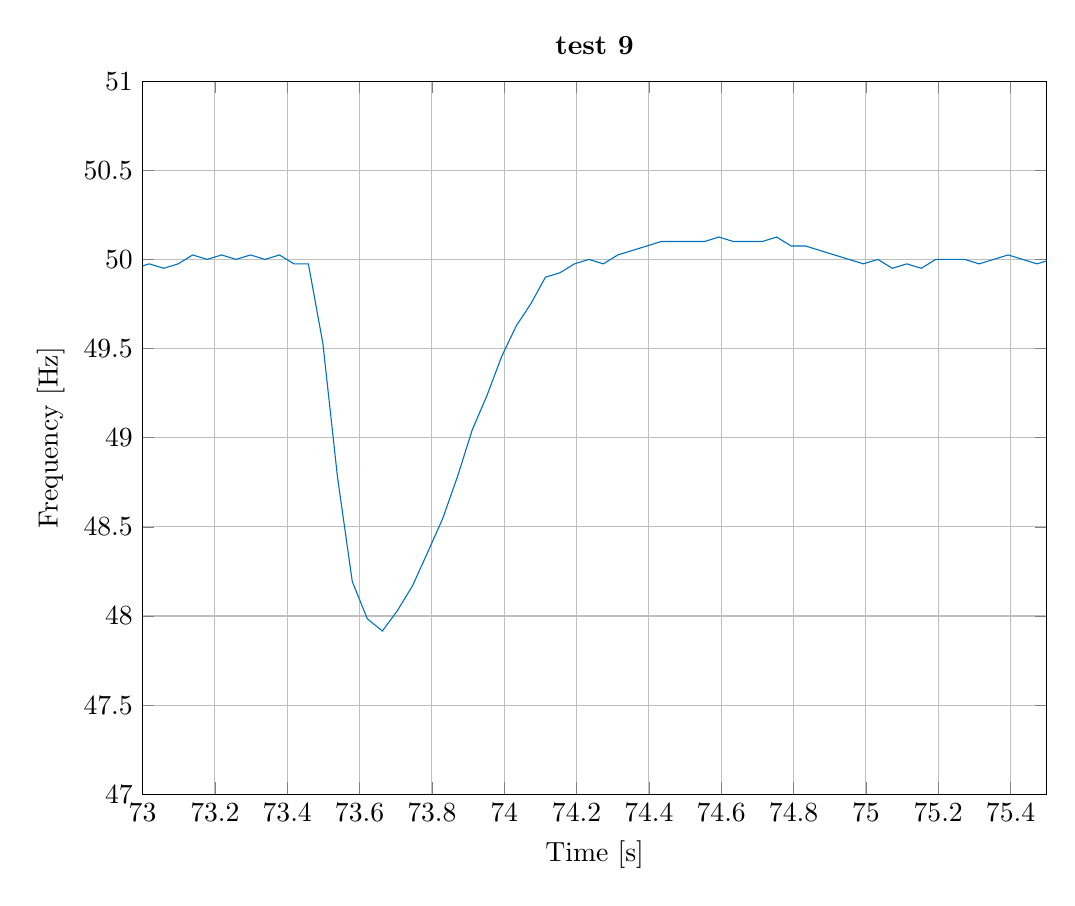
\begin{tikzpicture}

\begin{axis}[%
width=4.521in,
height=3.566in,
at={(0.758in,0.481in)},
scale only axis,
xmin=73,
xmax=75.5,
xlabel={Time [s]},
xmajorgrids,
ymin=47,
ymax=51,
ylabel={Frequency [Hz]},
ymajorgrids,
axis background/.style={fill=white},
title style={font=\bfseries},
title={test 9}
]
\addplot [color=mycolor1,solid,forget plot]
  table[row sep=crcr]{%
72.97846	49.950049950044\\
73.0185	49.9750124937551\\
73.05852	49.950049950044\\
73.09856	49.9750124937551\\
73.13858	50.0250125062532\\
73.17856	49.9999999999922\\
73.21856	50.025012506271\\
73.25854	49.9999999999922\\
73.29854	50.0250125062532\\
73.33852	50.0000000000099\\
73.37852	50.0250125062355\\
73.4185	49.9750124937551\\
73.45852	49.9750124937551\\
73.49854	49.5294700346719\\
73.53892	48.7804878048818\\
73.57992	48.1927710843383\\
73.62142	47.9846449136282\\
73.6631	47.9156684235695\\
73.70484	48.0307396733898\\
73.74648	48.1695568400871\\
73.788	48.3558994197322\\
73.82936	48.5436893203843\\
73.87056	48.7804878048818\\
73.91156	49.0436488474595\\
73.95234	49.2368291482151\\
73.99296	49.4559841740804\\
74.0334	49.627791563273\\
74.0737	49.7512437810962\\
74.1139	49.9001996007944\\
74.15398	49.9251123315066\\
74.19404	49.9750124937551\\
74.23406	49.9999999999922\\
74.27406	49.9750124937551\\
74.31408	50.0250125062532\\
74.35406	50.0500500500581\\
74.39402	50.0751126690017\\
74.43396	50.1002004008078\\
74.47388	50.10020040079\\
74.5138	50.1002004008078\\
74.55372	50.10020040079\\
74.59364	50.1253132832222\\
74.63354	50.10020040079\\
74.67346	50.1002004008078\\
74.71338	50.10020040079\\
74.7533	50.1253132832222\\
74.7932	50.0751126690017\\
74.83314	50.0751126690017\\
74.87308	50.0500500500403\\
74.91304	50.025012506271\\
74.95302	49.9999999999922\\
74.99302	49.9750124937551\\
75.03304	49.9999999999922\\
75.07304	49.950049950044\\
75.11308	49.9750124937551\\
75.1531	49.9500499500618\\
75.19314	49.9999999999922\\
75.23314	50.0000000000099\\
75.27314	49.9999999999922\\
75.31314	49.9750124937551\\
75.35316	49.9999999999922\\
75.39316	50.025012506271\\
75.43314	49.9999999999922\\
75.47314	49.9750124937551\\
75.51316	49.9999999999922\\
};
\end{axis}
\end{tikzpicture}%
\caption{Frequency disturbance on the output of the genset occuring from step of 30 to 50 kW load.}
\label{fig:test9-30to50kwstepfreq}
\end{figure}

\begin{figure}[H]
\centering
% This file was created by matlab2tikz.
%
%The latest updates can be retrieved from
%  http://www.mathworks.com/matlabcentral/fileexchange/22022-matlab2tikz-matlab2tikz
%where you can also make suggestions and rate matlab2tikz.
%
\definecolor{mycolor1}{rgb}{0.00000,0.44700,0.74100}%
%
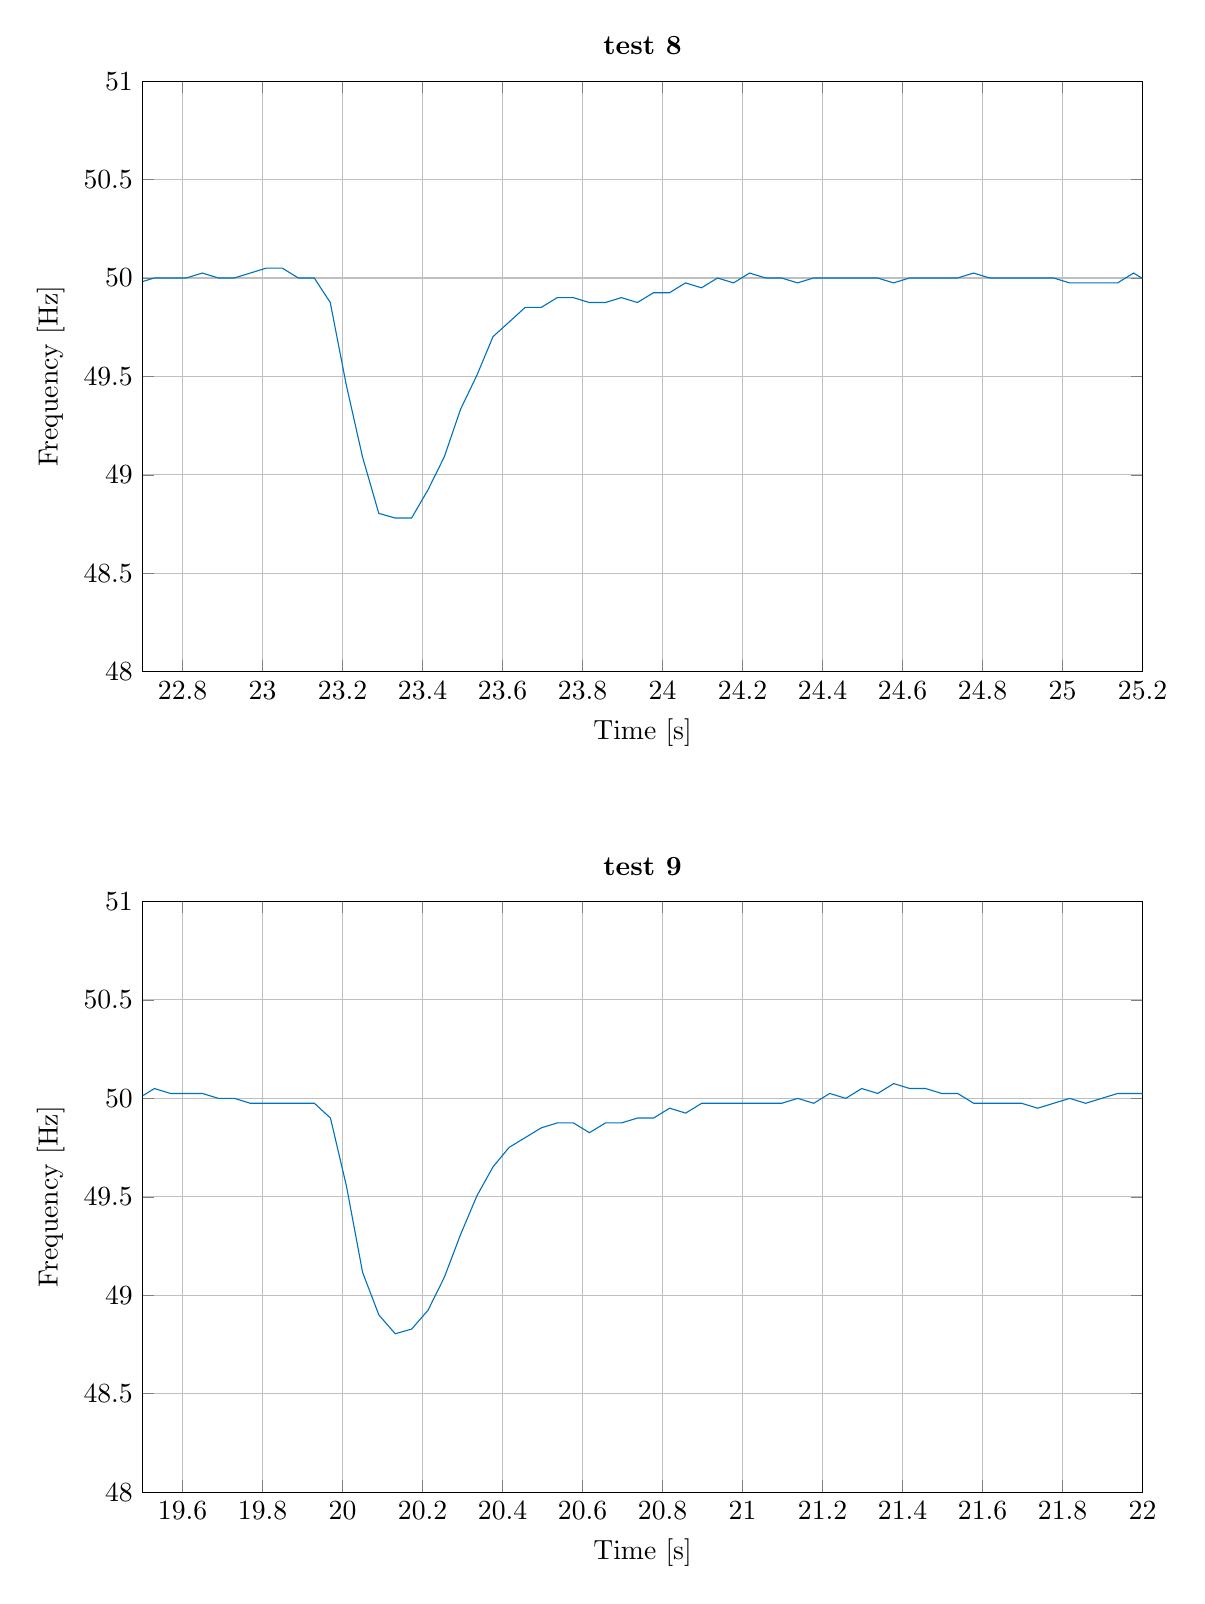
\begin{tikzpicture}

\begin{axis}[%
width=5in,
height=2.953in,
at={(1.142in,5.054in)},
scale only axis,
xmin=22.7,
xmax=25.2,
xlabel={Time [s]},
xmajorgrids,
ymin=48,
ymax=51,
ylabel={Frequency [Hz]},
ymajorgrids,
axis background/.style={fill=white},
title style={font=\bfseries},
title={test 8}
]
\addplot [color=mycolor1,solid,forget plot]
  table[row sep=crcr]{%
22.6894	49.9750124937551\\
22.72942	50.0000000000011\\
22.76942	49.9999999999966\\
22.80942	50.0000000000011\\
22.84942	50.0250125062532\\
22.8894	50.0000000000011\\
22.9294	50.0000000000011\\
22.9694	50.0250125062532\\
23.00938	50.0500500500492\\
23.04934	50.0500500500492\\
23.0893	50.0000000000011\\
23.1293	50.0000000000011\\
23.1693	49.8753117206952\\
23.2094	49.4559841740848\\
23.24984	49.0918016691218\\
23.29058	48.8042947779391\\
23.33156	48.7804878048818\\
23.37256	48.7804878048776\\
23.41356	48.9236790606637\\
23.45444	49.0918016691218\\
23.49518	49.3339911198816\\
23.53572	49.5049504950473\\
23.57612	49.701789264417\\
23.61636	49.7760079641576\\
23.65654	49.8504486540402\\
23.69666	49.8504486540358\\
23.73678	49.9001996007988\\
23.77686	49.9001996007988\\
23.81694	49.8753117206996\\
23.85704	49.8753117206996\\
23.89714	49.9001996007988\\
23.93722	49.8753117206952\\
23.97732	49.9251123315022\\
24.01738	49.9251123315066\\
24.05744	49.9750124937507\\
24.09746	49.9500499500485\\
24.1375	50.0000000000011\\
24.1775	49.9750124937551\\
24.21752	50.0250125062532\\
24.2575	49.9999999999966\\
24.2975	50.0000000000011\\
24.3375	49.9750124937551\\
24.37752	50.0000000000011\\
24.41752	49.9999999999966\\
24.45752	50.0000000000011\\
24.49752	50.0000000000011\\
24.53752	50.0000000000011\\
24.57752	49.9750124937507\\
24.61754	50.0000000000011\\
24.65754	50.0000000000011\\
24.69754	49.9999999999966\\
24.73754	50.0000000000011\\
24.77754	50.0250125062532\\
24.81752	50.0000000000011\\
24.85752	50.0000000000011\\
24.89752	49.9999999999966\\
24.93752	50.0000000000011\\
24.97752	50.0000000000011\\
25.01752	49.9750124937507\\
25.05754	49.9750124937551\\
25.09756	49.9750124937551\\
25.13758	49.9750124937507\\
25.1776	50.0250125062532\\
25.21758	49.9750124937551\\
};
\end{axis}

\begin{axis}[%
width=5in,
height=2.953in,
at={(1.142in,0.952in)},
scale only axis,
xmin=19.5,
xmax=22,
xlabel={Time [s]},
xmajorgrids,
ymin=48,
ymax=51,
ylabel={Frequency [Hz]},
ymajorgrids,
axis background/.style={fill=white},
title style={font=\bfseries},
title={test 9}
]
\addplot [color=mycolor1,solid,forget plot]
  table[row sep=crcr]{%
19.4897	50.0000000000011\\
19.5297	50.0500500500492\\
19.56966	50.0250125062532\\
19.60964	50.0250125062532\\
19.64962	50.0250125062532\\
19.6896	50.0000000000011\\
19.7296	50.0000000000011\\
19.7696	49.9750124937507\\
19.80962	49.9750124937551\\
19.84964	49.9750124937507\\
19.88966	49.9750124937551\\
19.92968	49.9750124937507\\
19.9697	49.9001996007988\\
20.00978	49.5540138751242\\
20.05014	49.1159135559918\\
20.09086	48.8997555012218\\
20.13176	48.8042947779433\\
20.17274	48.8281249999978\\
20.2137	48.923679060668\\
20.25458	49.0918016691218\\
20.29532	49.3096646942767\\
20.33588	49.5049504950517\\
20.37628	49.6524329692165\\
20.41656	49.7512437810918\\
20.45676	49.8007968127488\\
20.49692	49.8504486540402\\
20.53704	49.8753117206996\\
20.57714	49.8753117206952\\
20.61724	49.8256103637258\\
20.65738	49.8753117206996\\
20.69748	49.8753117206996\\
20.73758	49.9001996007988\\
20.77766	49.9001996007988\\
20.81774	49.9500499500485\\
20.85778	49.9251123315022\\
20.89784	49.9750124937551\\
20.93786	49.9750124937507\\
20.97788	49.9750124937551\\
21.0179	49.9750124937507\\
21.05792	49.9750124937551\\
21.09794	49.9750124937507\\
21.13796	50.0000000000011\\
21.17796	49.9750124937551\\
21.21798	50.0250125062532\\
21.25796	49.9999999999966\\
21.29796	50.0500500500537\\
21.33792	50.0250125062532\\
21.3779	50.0751126690017\\
21.41784	50.0500500500492\\
21.4578	50.0500500500492\\
21.49776	50.0250125062532\\
21.53774	50.0250125062532\\
21.57772	49.9750124937551\\
21.61774	49.9750124937507\\
21.65776	49.9750124937551\\
21.69778	49.9750124937551\\
21.7378	49.9500499500485\\
21.77784	49.9750124937507\\
21.81786	50.0000000000011\\
21.85786	49.9750124937551\\
21.89788	49.9999999999966\\
21.93788	50.0250125062532\\
21.97786	50.0250125062532\\
22.01784	50.0250125062532\\
};
\end{axis}
\end{tikzpicture}%
\caption{Frequency disturbance on the output of the genset occuring from step of 20 to 30 kW load.}
\label{fig:test8-9-20to30kwstepfreq}
\end{figure}

\begin{figure}[H]
\centering
% This file was created by matlab2tikz.
%
%The latest updates can be retrieved from
%  http://www.mathworks.com/matlabcentral/fileexchange/22022-matlab2tikz-matlab2tikz
%where you can also make suggestions and rate matlab2tikz.
%
\definecolor{mycolor1}{rgb}{0.00000,0.44700,0.74100}%
%
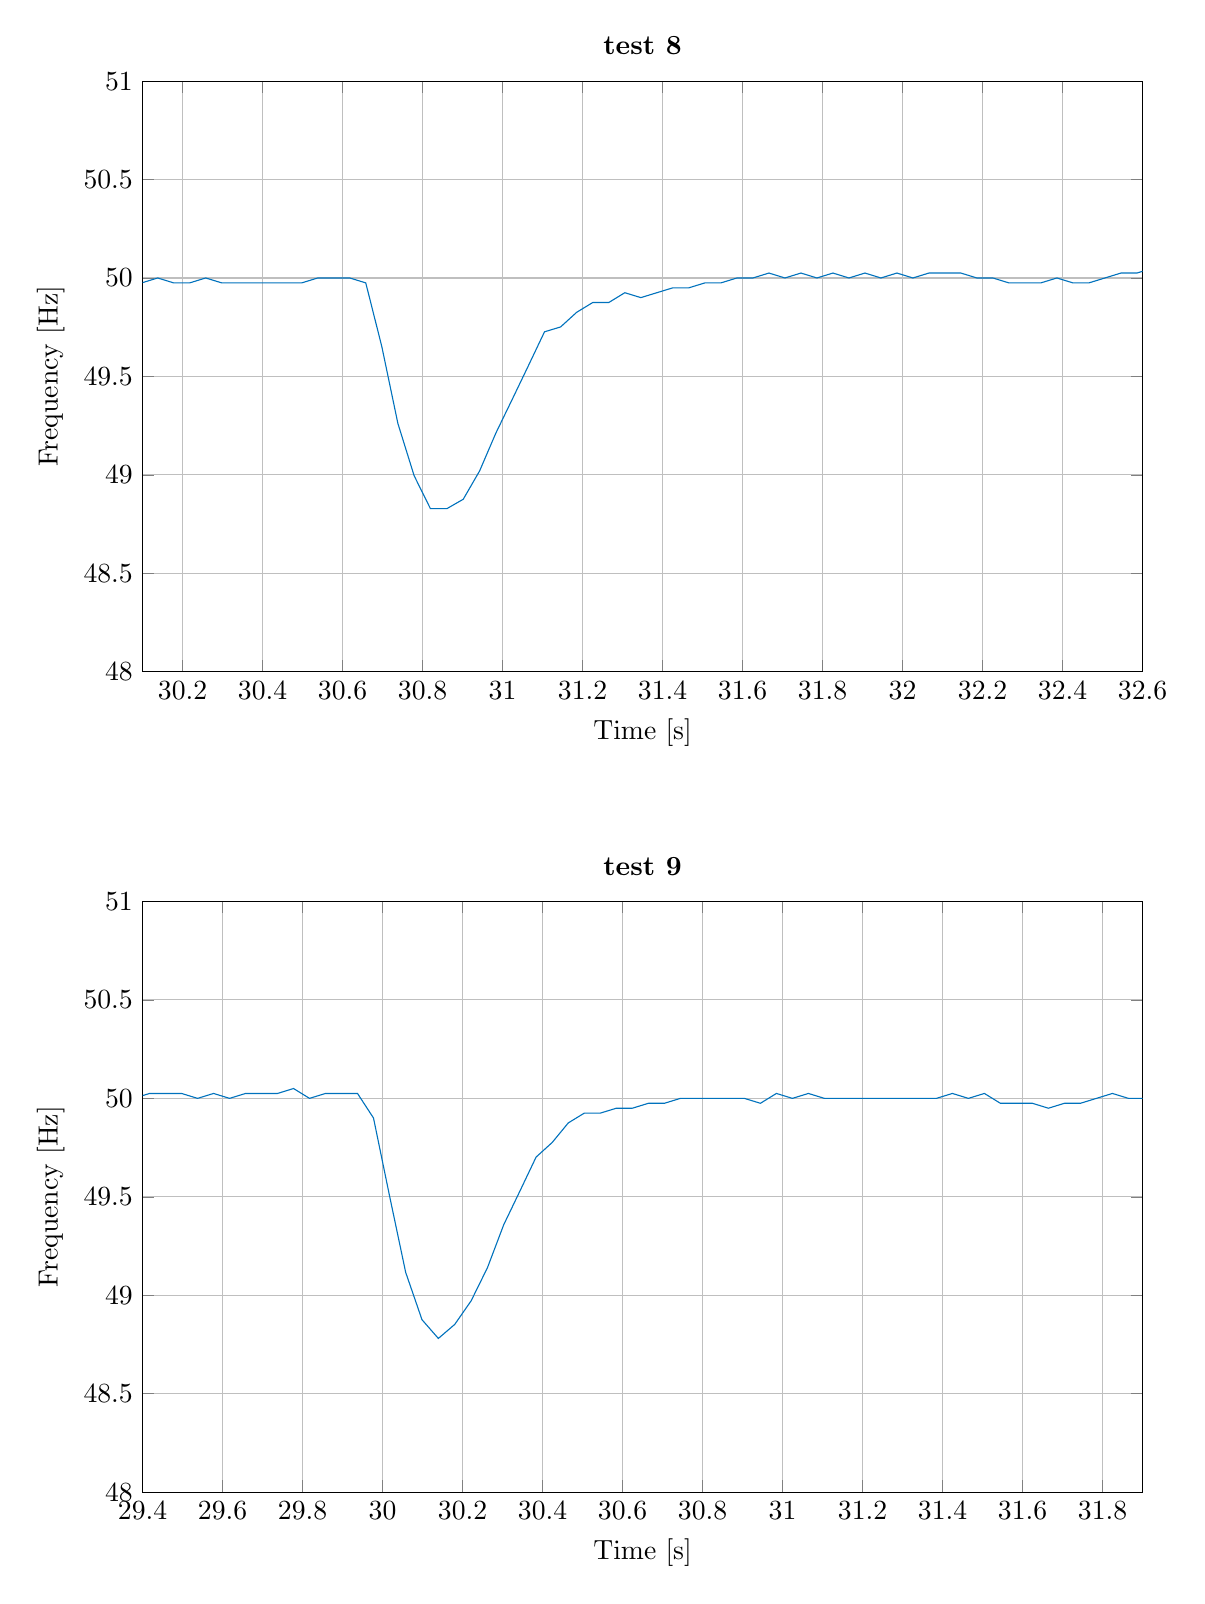
\begin{tikzpicture}

\begin{axis}[%
width=5in,
height=2.953in,
at={(1.142in,5.054in)},
scale only axis,
xmin=30.1,
xmax=32.6,
xlabel={Time [s]},
xmajorgrids,
ymin=48,
ymax=51,
ylabel={Frequency [Hz]},
ymajorgrids,
axis background/.style={fill=white},
title style={font=\bfseries},
title={test 8}
]
\addplot [color=mycolor1,solid,forget plot]
  table[row sep=crcr]{%
30.09786	49.9750124937507\\
30.13788	50.0000000000011\\
30.17788	49.9750124937551\\
30.2179	49.9750124937507\\
30.25792	50.0000000000011\\
30.29792	49.9750124937551\\
30.33794	49.9750124937507\\
30.37796	49.9750124937551\\
30.41798	49.9750124937507\\
30.458	49.9750124937551\\
30.49802	49.9750124937507\\
30.53804	50.0000000000011\\
30.57804	50.0000000000011\\
30.61804	50.0000000000011\\
30.65804	49.9750124937507\\
30.69806	49.6524329692165\\
30.73834	49.2610837438408\\
30.77894	48.9955903968642\\
30.81976	48.828125000002\\
30.86072	48.8281249999978\\
30.90168	48.8758553274684\\
30.9426	49.0196078431405\\
30.9834	49.2125984251971\\
31.02404	49.3827160493808\\
31.06454	49.5540138751242\\
31.1049	49.726504226751\\
31.14512	49.7512437810962\\
31.18532	49.8256103637258\\
31.22546	49.8753117206996\\
31.26556	49.8753117206996\\
31.30566	49.9251123315022\\
31.34572	49.9001996007988\\
31.3858	49.9251123315022\\
31.42586	49.9500499500485\\
31.4659	49.9500499500485\\
31.50594	49.9750124937551\\
31.54596	49.9750124937551\\
31.58598	49.9999999999966\\
31.62598	50.0000000000011\\
31.66598	50.0250125062532\\
31.70596	50.0000000000011\\
31.74596	50.0250125062532\\
31.78594	50.0000000000011\\
31.82594	50.0250125062532\\
31.86592	49.9999999999966\\
31.90592	50.0250125062532\\
31.9459	50.0000000000011\\
31.9859	50.0250125062577\\
32.02588	49.9999999999922\\
32.06588	50.0250125062532\\
32.10586	50.0250125062532\\
32.14584	50.0250125062532\\
32.18582	50.0000000000011\\
32.22582	50.0000000000011\\
32.26582	49.9750124937551\\
32.30584	49.9750124937551\\
32.34586	49.9750124937463\\
32.38588	50.0000000000011\\
32.42588	49.9750124937551\\
32.4659	49.9750124937551\\
32.50592	50.0000000000011\\
32.54592	50.0250125062532\\
32.5859	50.0250125062532\\
32.62588	50.0500500500492\\
};
\end{axis}

\begin{axis}[%
width=5in,
height=2.953in,
at={(1.142in,0.952in)},
scale only axis,
xmin=29.4,
xmax=31.9,
xlabel={Time [s]},
xmajorgrids,
ymin=48,
ymax=51,
ylabel={Frequency [Hz]},
ymajorgrids,
axis background/.style={fill=white},
title style={font=\bfseries},
title={test 9}
]
\addplot [color=mycolor1,solid,forget plot]
  table[row sep=crcr]{%
29.37762	50.0000000000011\\
29.41762	50.0250125062532\\
29.4576	50.0250125062532\\
29.49758	50.0250125062488\\
29.53756	50.0000000000011\\
29.57756	50.0250125062532\\
29.61754	50.0000000000011\\
29.65754	50.0250125062532\\
29.69752	50.0250125062532\\
29.7375	50.0250125062532\\
29.77748	50.0500500500492\\
29.81744	50.0000000000011\\
29.85744	50.0250125062532\\
29.89742	50.0250125062532\\
29.9374	50.0250125062532\\
29.97738	49.9001996007988\\
30.01746	49.5049504950473\\
30.05786	49.1159135559918\\
30.09858	48.8758553274684\\
30.1395	48.7804878048776\\
30.1805	48.8519785051305\\
30.22144	48.9715964740459\\
30.26228	49.1400491400479\\
30.30298	49.3583415597226\\
30.3435	49.5294700346719\\
30.38388	49.7017892644126\\
30.42412	49.776007964162\\
30.4643	49.8753117206996\\
30.5044	49.9251123315022\\
30.54446	49.9251123315022\\
30.58452	49.9500499500485\\
30.62456	49.9500499500529\\
30.6646	49.9750124937507\\
30.70462	49.9750124937551\\
30.74464	50.0000000000011\\
30.78464	49.9999999999966\\
30.82464	50.0000000000011\\
30.86464	50.0000000000011\\
30.90464	50.0000000000011\\
30.94464	49.9750124937507\\
30.98466	50.0250125062532\\
31.02464	50.0000000000011\\
31.06464	50.0250125062532\\
31.10462	50.0000000000011\\
31.14462	49.9999999999966\\
31.18462	50.0000000000011\\
31.22462	50.0000000000011\\
31.26462	50.0000000000011\\
31.30462	50.0000000000011\\
31.34462	49.9999999999966\\
31.38462	50.0000000000011\\
31.42462	50.0250125062532\\
31.4646	50.0000000000011\\
31.5046	50.0250125062532\\
31.54458	49.9750124937507\\
31.5846	49.9750124937551\\
31.62462	49.9750124937507\\
31.66464	49.9500499500529\\
31.70468	49.9750124937507\\
31.7447	49.9750124937551\\
31.78472	50.0000000000011\\
31.82472	50.0250125062532\\
31.8647	49.9999999999966\\
31.9047	50.0000000000011\\
};
\end{axis}
\end{tikzpicture}%
\caption{Frequency disturbance on the output of the genset occuring from step of 30 to 40 kW load.}
\label{fig:test8-9-30to40kwstepfreq}
\end{figure}

\begin{figure}[H]
\centering
% This file was created by matlab2tikz.
%
%The latest updates can be retrieved from
%  http://www.mathworks.com/matlabcentral/fileexchange/22022-matlab2tikz-matlab2tikz
%where you can also make suggestions and rate matlab2tikz.
%
\definecolor{mycolor1}{rgb}{0.00000,0.44700,0.74100}%
%
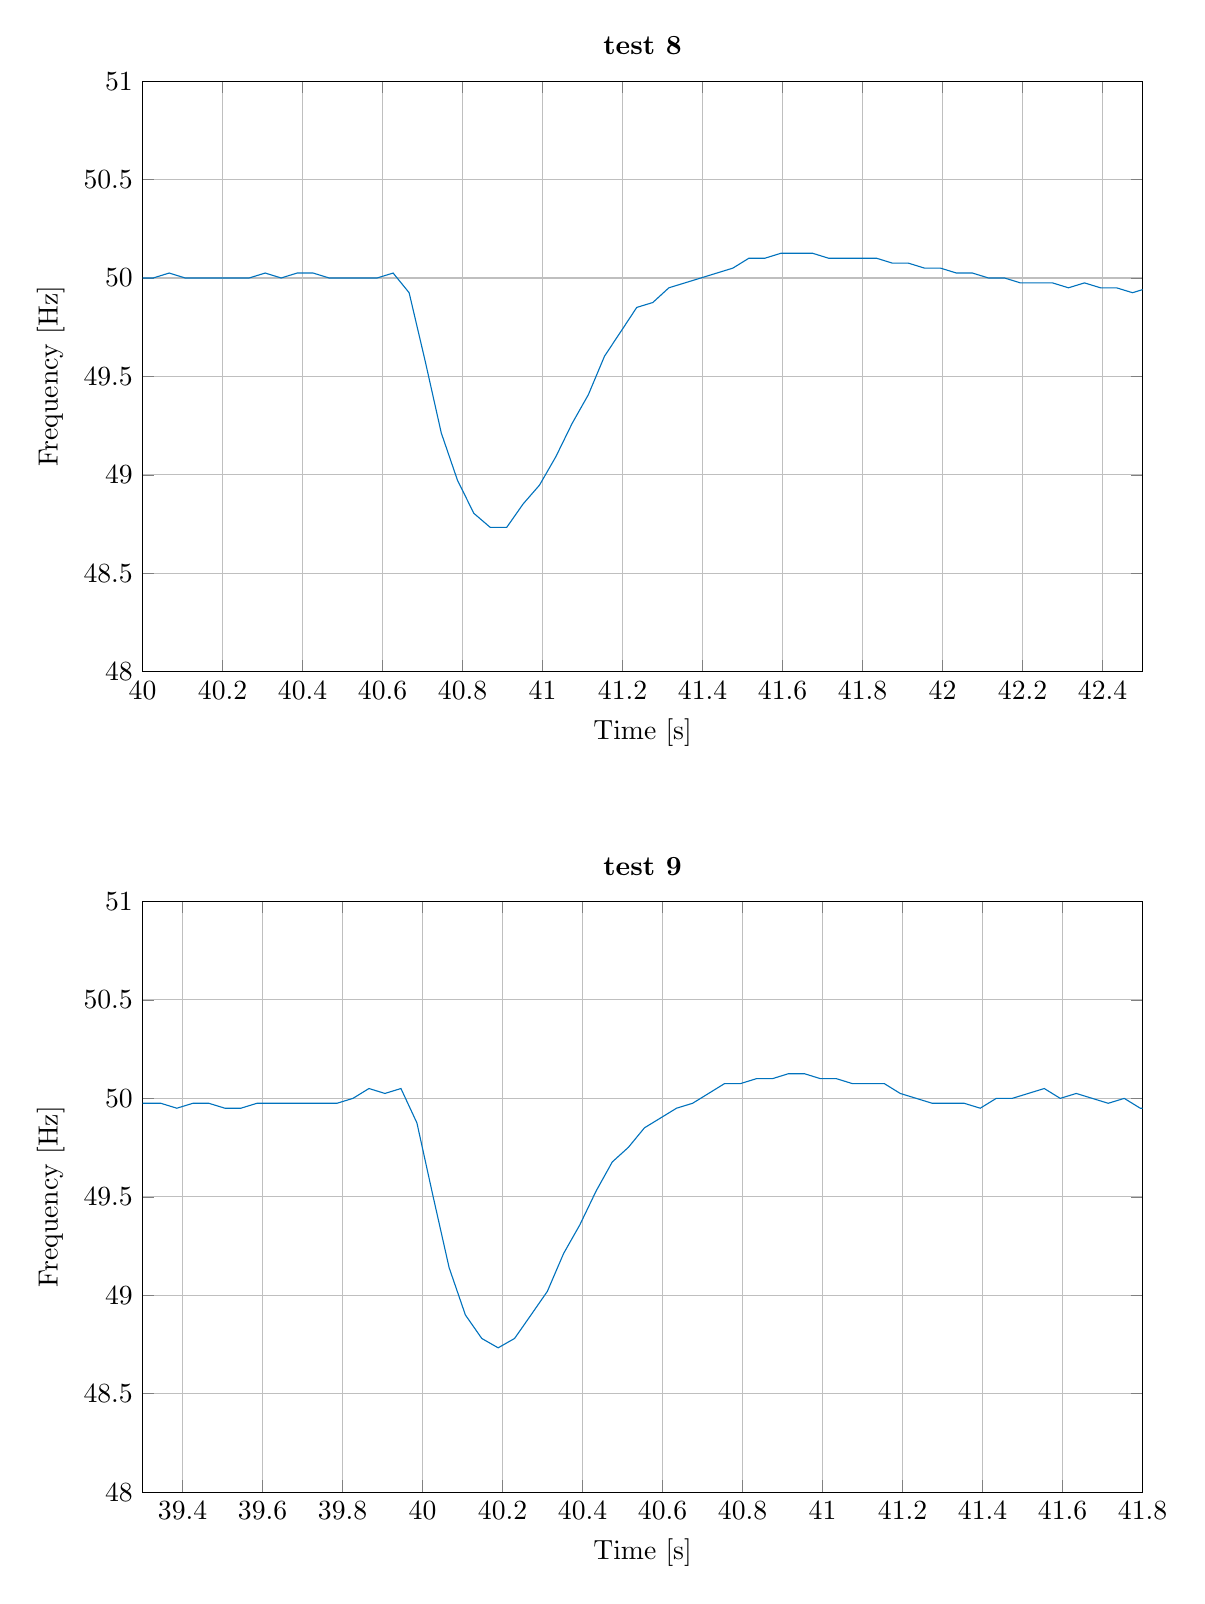
\begin{tikzpicture}

\begin{axis}[%
width=5in,
height=2.953in,
at={(1.142in,5.054in)},
scale only axis,
xmin=40,
xmax=42.5,
xlabel={Time [s]},
xmajorgrids,
ymin=48,
ymax=51,
ylabel={Frequency [Hz]},
ymajorgrids,
axis background/.style={fill=white},
title style={font=\bfseries},
title={test 8}
]
\addplot [color=mycolor1,solid,forget plot]
  table[row sep=crcr]{%
39.98654	50.0000000000011\\
40.02654	50.0000000000011\\
40.06654	50.0250125062532\\
40.10652	50.0000000000011\\
40.14652	50.0000000000011\\
40.18652	50.0000000000011\\
40.22652	49.9999999999922\\
40.26652	50.0000000000011\\
40.30652	50.0250125062532\\
40.3465	50.0000000000011\\
40.3865	50.0250125062532\\
40.42648	50.0250125062532\\
40.46646	50.0000000000011\\
40.50646	50.0000000000011\\
40.54646	50.0000000000011\\
40.58646	50.0000000000011\\
40.62646	50.0250125062532\\
40.66644	49.9251123314978\\
40.7065	49.5785820525527\\
40.74684	49.2125984252014\\
40.78748	48.9715964740416\\
40.82832	48.8042947779433\\
40.8693	48.7329434697827\\
40.91034	48.7329434697912\\
40.95138	48.8519785051221\\
40.99232	48.947626040143\\
41.03318	49.0918016691218\\
41.07392	49.2610837438365\\
41.11452	49.4071146245118\\
41.155	49.6031746031731\\
41.19532	49.7265042267554\\
41.23554	49.8504486540358\\
41.27566	49.8753117206952\\
41.31576	49.9500499500529\\
41.3558	49.9750124937551\\
41.39582	49.9999999999922\\
41.43582	50.0250125062532\\
41.4758	50.0500500500581\\
41.51576	50.1002004007989\\
41.55568	50.1002004007989\\
41.5956	50.1253132832133\\
41.6355	50.1253132832043\\
41.6754	50.1253132832043\\
41.7153	50.1002004008078\\
41.75522	50.1002004007989\\
41.79514	50.1002004007989\\
41.83506	50.1002004008078\\
41.87498	50.0751126690017\\
41.91492	50.0751126690017\\
41.95486	50.0500500500492\\
41.99482	50.0500500500492\\
42.03478	50.0250125062532\\
42.07476	50.0250125062532\\
42.11474	50.0000000000011\\
42.15474	50.0000000000011\\
42.19474	49.9750124937551\\
42.23476	49.9750124937463\\
42.27478	49.9750124937551\\
42.3148	49.9500499500529\\
42.35484	49.9750124937551\\
42.39486	49.950049950044\\
42.4349	49.9500499500529\\
42.47494	49.9251123315066\\
42.515	49.950049950044\\
};
\end{axis}

\begin{axis}[%
width=5in,
height=2.953in,
at={(1.142in,0.952in)},
scale only axis,
xmin=39.3,
xmax=41.8,
xlabel={Time [s]},
xmajorgrids,
ymin=48,
ymax=51,
ylabel={Frequency [Hz]},
ymajorgrids,
axis background/.style={fill=white},
title style={font=\bfseries},
title={test 9}
]
\addplot [color=mycolor1,solid,forget plot]
  table[row sep=crcr]{%
39.2657	49.9750124937551\\
39.30572	49.9750124937463\\
39.34574	49.9750124937551\\
39.38576	49.9500499500529\\
39.4258	49.9750124937551\\
39.46582	49.9750124937463\\
39.50584	49.9500499500529\\
39.54588	49.9500499500529\\
39.58592	49.9750124937463\\
39.62594	49.9750124937551\\
39.66596	49.9750124937551\\
39.70598	49.9750124937551\\
39.746	49.9750124937551\\
39.78602	49.9750124937463\\
39.82604	50.0000000000011\\
39.86604	50.0500500500492\\
39.906	50.0250125062532\\
39.94598	50.0500500500492\\
39.98594	49.875311720704\\
40.02604	49.5049504950517\\
40.06644	49.1400491400479\\
40.10714	48.8997555012218\\
40.14804	48.7804878048734\\
40.18904	48.7329434697912\\
40.23008	48.7804878048734\\
40.27108	48.8997555012218\\
40.31198	49.0196078431405\\
40.35278	49.2125984251928\\
40.39342	49.3583415597226\\
40.43394	49.5294700346719\\
40.47432	49.6770988574312\\
40.51458	49.7512437810962\\
40.55478	49.8504486540358\\
40.5949	49.9001996007944\\
40.63498	49.9500499500529\\
40.67502	49.9750124937551\\
40.71504	50.0250125062532\\
40.75502	50.0751126690017\\
40.79496	50.0751126690017\\
40.8349	50.1002004007989\\
40.87482	50.1002004008078\\
40.91474	50.1253132832043\\
40.95464	50.1253132832133\\
40.99454	50.1002004007989\\
41.03446	50.1002004007989\\
41.07438	50.0751126690017\\
41.11432	50.0751126690106\\
41.15426	50.0751126690017\\
41.1942	50.0250125062532\\
41.23418	50.0000000000011\\
41.27418	49.9750124937463\\
41.3142	49.9750124937551\\
41.35422	49.9750124937551\\
41.39424	49.9500499500529\\
41.43428	50.0000000000011\\
41.47428	49.9999999999922\\
41.51428	50.0250125062532\\
41.55426	50.0500500500581\\
41.59422	49.9999999999922\\
41.63422	50.0250125062532\\
41.6742	50.0000000000011\\
41.7142	49.9750124937551\\
41.75422	50.0000000000011\\
41.79422	49.9500499500529\\
41.83426	49.950049950044\\
};
\end{axis}
\end{tikzpicture}%
\caption{Frequency disturbance on the output of the genset occuring from step of 40 to 50 kW load.}
\label{fig:test8-9-40to50kwstepfreq}
\end{figure}

\begin{figure}[H]
\centering
% This file was created by matlab2tikz.
%
%The latest updates can be retrieved from
%  http://www.mathworks.com/matlabcentral/fileexchange/22022-matlab2tikz-matlab2tikz
%where you can also make suggestions and rate matlab2tikz.
%
\definecolor{mycolor1}{rgb}{0.00000,0.44700,0.74100}%
%
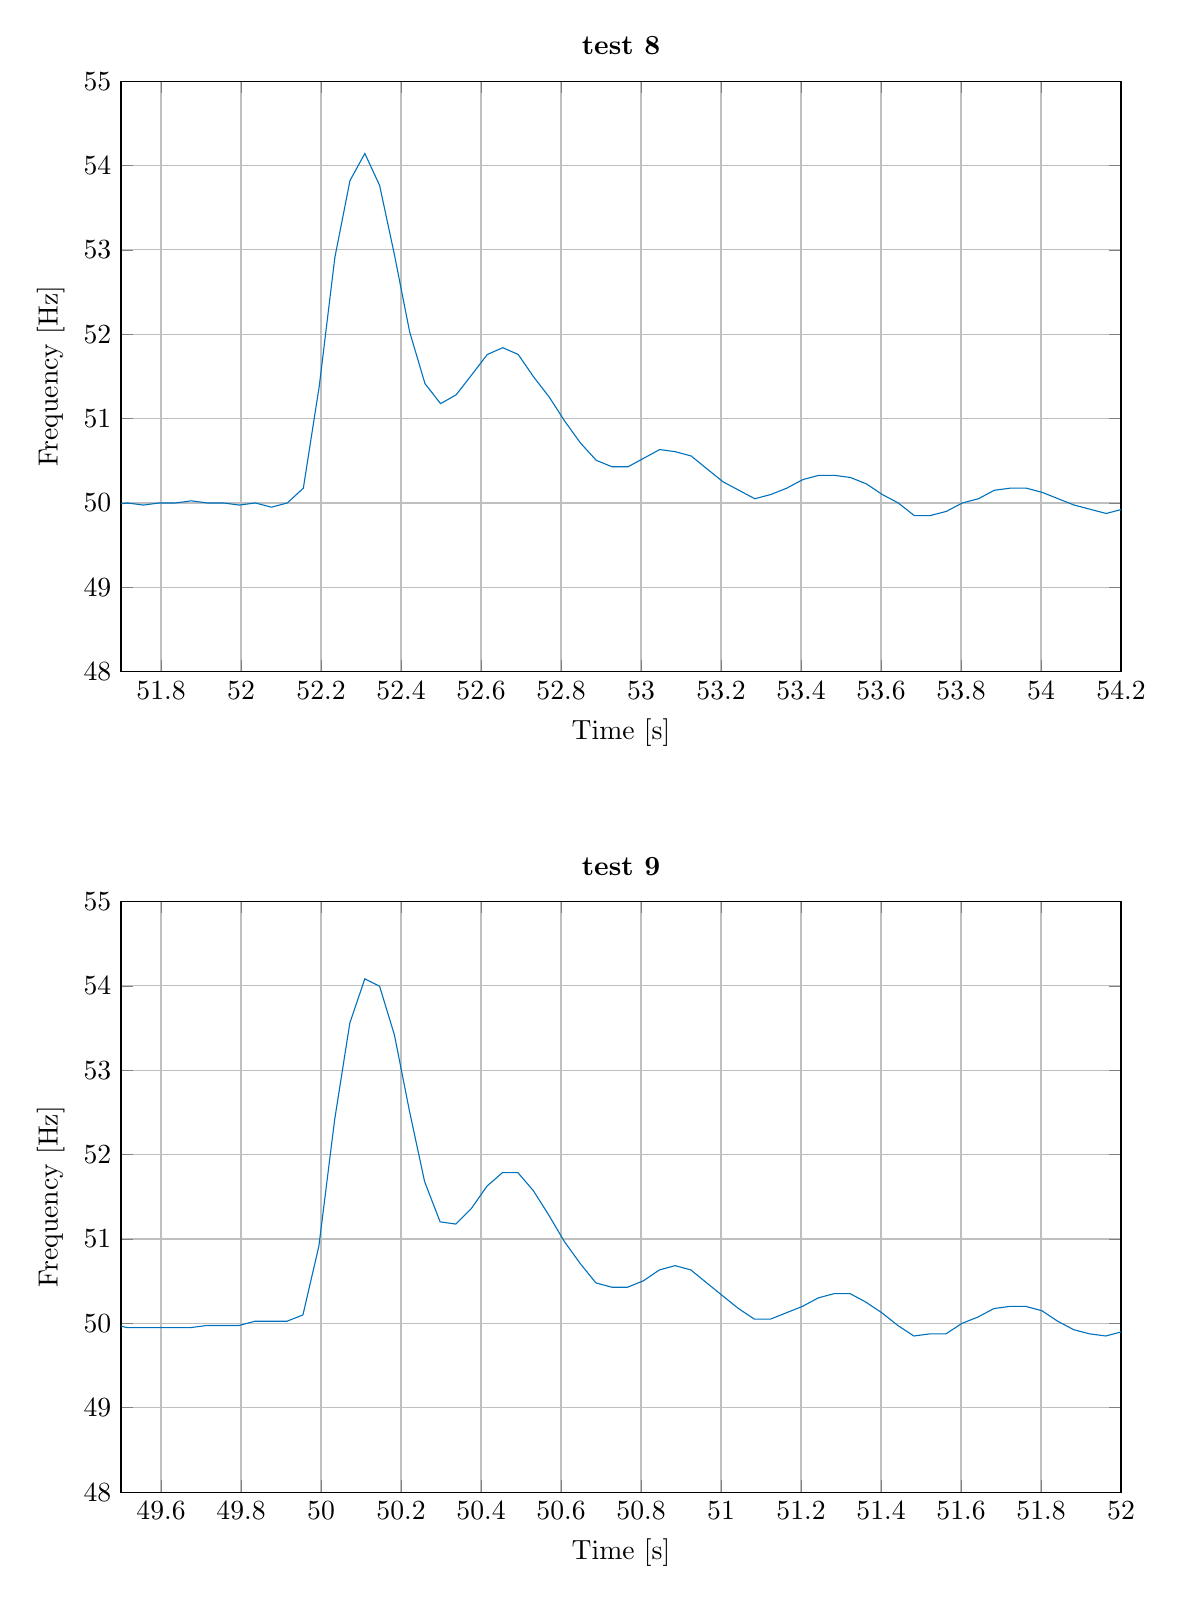
\begin{tikzpicture}

\begin{axis}[%
width=5in,
height=2.953in,
at={(1.142in,5.054in)},
scale only axis,
xmin=51.7,
xmax=54.2,
xlabel={Time [s]},
xmajorgrids,
ymin=48,
ymax=55,
ylabel={Frequency [Hz]},
ymajorgrids,
axis background/.style={fill=white},
title style={font=\bfseries},
title={test 8}
]
\addplot [color=mycolor1,solid,forget plot]
  table[row sep=crcr]{%
51.67574	49.9750124937551\\
51.71576	50.0000000000011\\
51.75576	49.9750124937463\\
51.79578	50.0000000000011\\
51.83578	50.0000000000011\\
51.87578	50.0250125062532\\
51.91576	50.0000000000011\\
51.95576	50.0000000000011\\
51.99576	49.9750124937551\\
52.03578	50.0000000000011\\
52.07578	49.950049950044\\
52.11582	50.0000000000011\\
52.15582	50.1756146512828\\
52.19568	51.387461459398\\
52.2346	52.9100529100569\\
52.2724	53.8213132400429\\
52.30956	54.1418516513246\\
52.3465	53.7634408602171\\
52.3837	52.9380624669166\\
52.42148	52.0291363163353\\
52.45992	51.4138817480744\\
52.49882	51.1770726714359\\
52.5379	51.2820512820587\\
52.5769	51.519835136526\\
52.61572	51.7598343685288\\
52.65436	51.8403317781191\\
52.69294	51.7598343685383\\
52.73158	51.4933058702363\\
52.77042	51.2557662737048\\
52.80944	50.9683995922535\\
52.84868	50.7099391480743\\
52.88812	50.5050505050504\\
52.92772	50.4286434694844\\
52.96738	50.4286434694935\\
53.00704	50.5305709954512\\
53.04662	50.6329113924092\\
53.08612	50.6072874493887\\
53.12564	50.5561172901901\\
53.1652	50.4032258064554\\
53.20488	50.2512562814075\\
53.24468	50.1504513540575\\
53.28456	50.0500500500492\\
53.32452	50.1002004008078\\
53.36444	50.1756146512739\\
53.4043	50.2765208647557\\
53.44408	50.3271263210937\\
53.48382	50.3271263210847\\
53.52356	50.3018108651897\\
53.56332	50.2260170768472\\
53.60314	50.1002004007989\\
53.64306	50.0000000000011\\
53.68306	49.8504486540358\\
53.72318	49.8504486540446\\
53.7633	49.9001996007944\\
53.80338	50.0000000000011\\
53.84338	50.0500500500492\\
53.88334	50.1504513540665\\
53.92322	50.1756146512739\\
53.96308	50.1756146512828\\
54.00294	50.1253132832043\\
54.04284	50.0500500500492\\
54.0828	49.9750124937551\\
54.12282	49.9251123315066\\
54.16288	49.8753117206952\\
54.20298	49.9251123315066\\
};
\end{axis}

\begin{axis}[%
width=5in,
height=2.953in,
at={(1.142in,0.952in)},
scale only axis,
xmin=49.5,
xmax=52,
xlabel={Time [s]},
xmajorgrids,
ymin=48,
ymax=55,
ylabel={Frequency [Hz]},
ymajorgrids,
axis background/.style={fill=white},
title style={font=\bfseries},
title={test 9}
]
\addplot [color=mycolor1,solid,forget plot]
  table[row sep=crcr]{%
49.47456	50.0000000000011\\
49.51456	49.9500499500529\\
49.5546	49.950049950044\\
49.59464	49.9500499500529\\
49.63468	49.9500499500529\\
49.67472	49.950049950044\\
49.71476	49.9750124937551\\
49.75478	49.9750124937551\\
49.7948	49.9750124937551\\
49.83482	50.0250125062532\\
49.8748	50.0250125062532\\
49.91478	50.0250125062532\\
49.95476	50.1002004007989\\
49.99468	50.9164969450128\\
50.03396	52.4109014675083\\
50.07212	53.561863952865\\
50.10946	54.0832882639268\\
50.14644	53.995680345576\\
50.18348	53.4188034187981\\
50.22092	52.5210084033603\\
50.259	51.6795865633093\\
50.2977	51.2032770097297\\
50.33676	51.1770726714452\\
50.37584	51.3610683102159\\
50.41478	51.6262261228743\\
50.45352	51.7866390471236\\
50.49214	51.7866390471332\\
50.53076	51.5729757606978\\
50.56954	51.2820512820493\\
50.60854	50.9683995922535\\
50.64778	50.7099391480743\\
50.68722	50.47955577991\\
50.72684	50.4286434694844\\
50.7665	50.4286434694935\\
50.80616	50.5050505050504\\
50.84576	50.6329113924092\\
50.88526	50.6842372022232\\
50.92472	50.6329113924092\\
50.96422	50.47955577991\\
51.00384	50.3271263210847\\
51.04358	50.1756146512828\\
51.08344	50.0500500500492\\
51.1234	50.0500500500492\\
51.16336	50.1253132832043\\
51.20326	50.2008032128538\\
51.2431	50.3018108651897\\
51.28286	50.3524672709019\\
51.32258	50.3524672708929\\
51.3623	50.2512562814075\\
51.4021	50.1253132832043\\
51.442	49.9750124937551\\
51.48202	49.8504486540358\\
51.52214	49.875311720704\\
51.56224	49.8753117206952\\
51.60234	50.0000000000011\\
51.64234	50.0751126690017\\
51.68228	50.1756146512828\\
51.72214	50.2008032128538\\
51.76198	50.2008032128448\\
51.80182	50.1504513540665\\
51.8417	50.0250125062532\\
51.88168	49.9251123314978\\
51.92174	49.875311720704\\
51.96184	49.8504486540358\\
52.00196	49.9001996007944\\
};
\end{axis}
\end{tikzpicture}%
\caption{Frequency disturbance on the output of the genset occuring from step of 50 to 10 kW load.}
\label{fig:test8-9-50to10kwstepfreq}
\end{figure}

%---------------------------------------------------
% \subsubsection*{Power}
% \begin{figure}[H]
% \centering
% % This file was created by matlab2tikz.
%
%The latest updates can be retrieved from
%  http://www.mathworks.com/matlabcentral/fileexchange/22022-matlab2tikz-matlab2tikz
%where you can also make suggestions and rate matlab2tikz.
%
\definecolor{mycolor1}{rgb}{0.00000,0.44700,0.74100}%
%
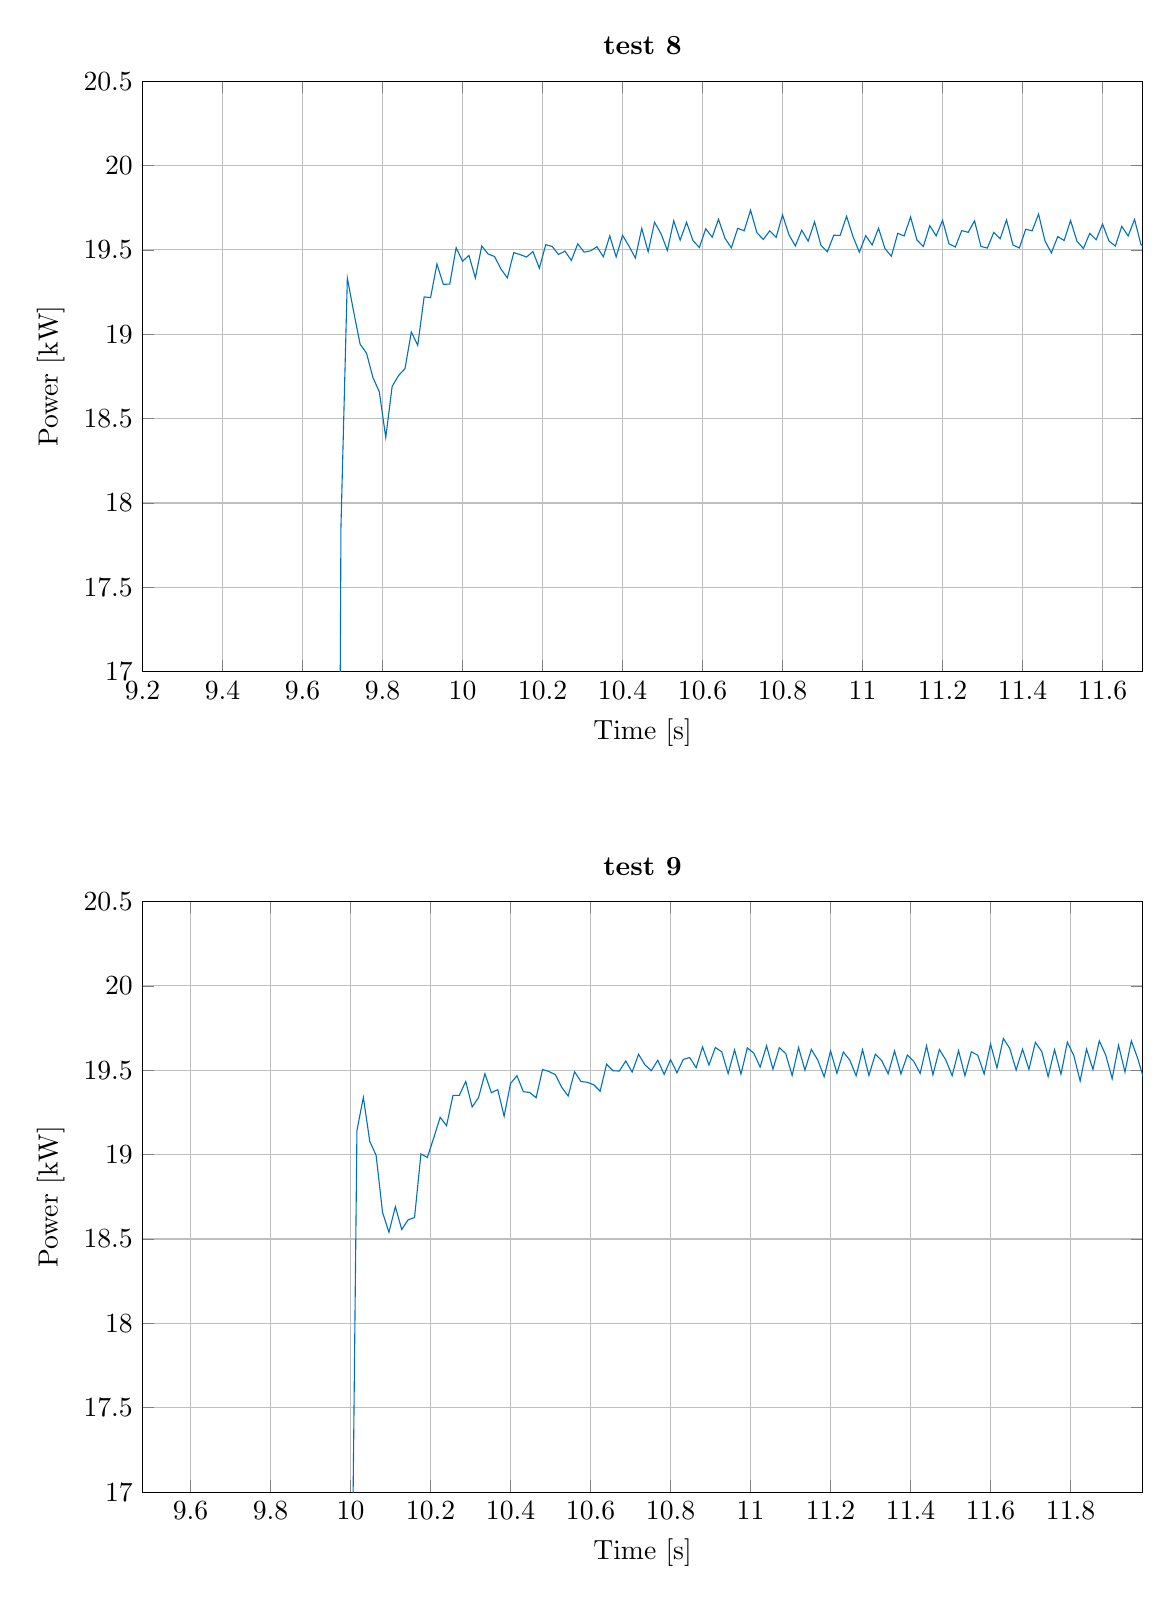
\begin{tikzpicture}

\begin{axis}[%
width=5in,
height=2.953in,
at={(1.142in,5.054in)},
scale only axis,
xmin=9.2,
xmax=11.7,
xlabel={Time [s]},
xmajorgrids,
ymin=17,
ymax=20.5,
ylabel={Power [kW]},
ymajorgrids,
axis background/.style={fill=white},
title style={font=\bfseries},
title={test 8}
]
\addplot [color=mycolor1,solid,forget plot]
  table[row sep=crcr]{%
9.69361195216867	16.65\\
9.696	17.8560997486441\\
9.712	19.3317559612937\\
9.728	19.1307270208216\\
9.744	18.9409069267782\\
9.76	18.8875421407511\\
9.776	18.7431518739233\\
9.792	18.6580033244411\\
9.808	18.3880309921695\\
9.824	18.6904882202812\\
9.84	18.7552111350607\\
9.856	18.7955140106475\\
9.872	19.0129382783991\\
9.888	18.9343650319984\\
9.904	19.2210665076048\\
9.92	19.2167144913738\\
9.936	19.4156547464794\\
9.952	19.2952832794037\\
9.968	19.2975176801068\\
9.984	19.5123085054123\\
10	19.4323669564606\\
10.016	19.4672267169912\\
10.032	19.3332590014944\\
10.048	19.5231456527388\\
10.064	19.4749948692252\\
10.08	19.4606409614458\\
10.096	19.3865656131167\\
10.112	19.3338865446942\\
10.128	19.4837888446628\\
10.144	19.4718180724555\\
10.16	19.4574234805144\\
10.176	19.4898686216038\\
10.192	19.3912814881103\\
10.208	19.5304982161064\\
10.224	19.520292915643\\
10.24	19.4725882575859\\
10.256	19.4924317464003\\
10.272	19.4371649821043\\
10.288	19.5355148706309\\
10.304	19.4864288899243\\
10.32	19.4939135331753\\
10.336	19.5182580959949\\
10.352	19.4590322056096\\
10.368	19.5826072302575\\
10.384	19.4582154847345\\
10.4	19.5858643622985\\
10.416	19.5227667828497\\
10.432	19.4517002419738\\
10.448	19.6268633227837\\
10.464	19.4888295559736\\
10.48	19.6631153925414\\
10.496	19.5968587468867\\
10.512	19.4964849877434\\
10.528	19.6724098941325\\
10.544	19.5575016738631\\
10.56	19.6629322751402\\
10.576	19.5551643953683\\
10.592	19.5138548618743\\
10.608	19.6250402299791\\
10.624	19.5745755904395\\
10.64	19.681491232703\\
10.656	19.5684888503774\\
10.672	19.5122630143226\\
10.688	19.6276248844025\\
10.704	19.6130119087638\\
10.72	19.7350838075075\\
10.736	19.6007978260301\\
10.752	19.561846992996\\
10.768	19.6128060413643\\
10.784	19.573915831523\\
10.8	19.7072299021751\\
10.816	19.58911378232\\
10.832	19.5234992085348\\
10.848	19.6161510835108\\
10.864	19.551376240204\\
10.88	19.6661859252241\\
10.896	19.5269185791918\\
10.912	19.4886353326526\\
10.928	19.5865038645685\\
10.944	19.5855779971464\\
10.96	19.698898756217\\
10.976	19.5795941146611\\
10.992	19.4861067370652\\
11.008	19.5840073018299\\
11.024	19.5292688925877\\
11.04	19.6283827177278\\
11.056	19.507475499928\\
11.072	19.461910622677\\
11.088	19.5979196594629\\
11.104	19.5823815857835\\
11.12	19.6950969284291\\
11.136	19.5586570784222\\
11.152	19.5201750954123\\
11.168	19.6434464050416\\
11.184	19.583192879939\\
11.2	19.6747972052404\\
11.216	19.5357851371188\\
11.232	19.5167691679337\\
11.248	19.6142828594775\\
11.264	19.6037949665122\\
11.28	19.6713079437157\\
11.296	19.5200100783074\\
11.312	19.5106695966919\\
11.328	19.6032265095905\\
11.344	19.5656769226009\\
11.36	19.6776852831439\\
11.376	19.5289110140086\\
11.392	19.5111452030148\\
11.408	19.6221473093952\\
11.424	19.6129697425636\\
11.44	19.711909239006\\
11.456	19.5532015819063\\
11.472	19.4822177885451\\
11.488	19.5787550250619\\
11.504	19.5553175497245\\
11.52	19.6739093631977\\
11.536	19.5511498936116\\
11.552	19.5080224374094\\
11.568	19.5973231153856\\
11.584	19.5600795025129\\
11.6	19.6525601985617\\
11.616	19.5524923998165\\
11.632	19.5226895699395\\
11.648	19.639260245484\\
11.664	19.5825400379335\\
11.68	19.6802942073984\\
11.696	19.5318485951422\\
11.712	19.4993715106933\\
};
\end{axis}

\begin{axis}[%
width=5in,
height=2.953in,
at={(1.142in,0.952in)},
scale only axis,
xmin=9.48,
xmax=11.98,
xlabel={Time [s]},
xmajorgrids,
ymin=17,
ymax=20.5,
ylabel={Power [kW]},
ymajorgrids,
axis background/.style={fill=white},
title style={font=\bfseries},
title={test 9}
]
\addplot [color=mycolor1,solid,forget plot]
  table[row sep=crcr]{%
10.0049151900697	16.65\\
10.016	19.1428483549108\\
10.032	19.3395075116513\\
10.048	19.0789632517411\\
10.064	18.9950185100708\\
10.08	18.6573875398207\\
10.096	18.539570101772\\
10.112	18.6913133104028\\
10.128	18.5561583000633\\
10.144	18.6135950731512\\
10.16	18.6271663393191\\
10.176	19.0040004177516\\
10.192	18.9831294600532\\
10.208	19.0992896815256\\
10.224	19.2210834643754\\
10.24	19.1713318793275\\
10.256	19.3510416866135\\
10.272	19.3512718128576\\
10.288	19.4341727943185\\
10.304	19.2821290959791\\
10.32	19.3380187075818\\
10.336	19.4797795304048\\
10.352	19.3665793778717\\
10.368	19.3851224044896\\
10.384	19.2278966519456\\
10.4	19.4216824810838\\
10.416	19.4673079344623\\
10.432	19.3731720619797\\
10.448	19.368118209495\\
10.464	19.3373937615391\\
10.48	19.5044968609124\\
10.496	19.4924406059497\\
10.512	19.4739710827107\\
10.528	19.3986697651543\\
10.544	19.3472717149574\\
10.56	19.491337232937\\
10.576	19.4334623426203\\
10.592	19.4285939916584\\
10.608	19.4138756661582\\
10.624	19.3761166500475\\
10.64	19.5351973723236\\
10.656	19.4971294040317\\
10.672	19.4952887604201\\
10.688	19.5548479013493\\
10.704	19.4894061246147\\
10.72	19.5945800610412\\
10.736	19.5318842812369\\
10.752	19.497929219753\\
10.768	19.5592883891434\\
10.784	19.4757777009216\\
10.8	19.5628215955071\\
10.816	19.4854158722045\\
10.832	19.5642547376548\\
10.848	19.5753630132049\\
10.864	19.515136057647\\
10.88	19.6379239296188\\
10.896	19.5308001655047\\
10.912	19.6349397635418\\
10.928	19.6091140313288\\
10.944	19.4801475731814\\
10.96	19.6210915007628\\
10.976	19.4773164772398\\
10.992	19.6329182902361\\
11.008	19.6016386370109\\
11.024	19.5189128581363\\
11.04	19.6453926428354\\
11.056	19.5062552267036\\
11.072	19.6337948480406\\
11.088	19.5985871637322\\
11.104	19.4694759529201\\
11.12	19.6344646441589\\
11.136	19.5010056600944\\
11.152	19.6235703018208\\
11.168	19.5608998763236\\
11.184	19.4613934051609\\
11.2	19.6144116530277\\
11.216	19.4823418321009\\
11.232	19.6078833844869\\
11.248	19.560517060277\\
11.264	19.4668628824997\\
11.28	19.62187541403\\
11.296	19.469136382854\\
11.312	19.5953232626741\\
11.328	19.556450242134\\
11.344	19.4787682899254\\
11.36	19.6145094829103\\
11.376	19.477555968219\\
11.392	19.5900038444707\\
11.408	19.5527800969042\\
11.424	19.4814532605605\\
11.44	19.6450624208517\\
11.456	19.4729518444822\\
11.472	19.6230297974097\\
11.488	19.5617547872651\\
11.504	19.4679066319098\\
11.52	19.6158824678861\\
11.536	19.4674717286468\\
11.552	19.6086704044808\\
11.568	19.5895396183913\\
11.584	19.4779958706679\\
11.6	19.6551180258722\\
11.616	19.5140537705196\\
11.632	19.6883453859425\\
11.648	19.6291325575914\\
11.664	19.5014852541641\\
11.68	19.6249289188855\\
11.696	19.5052119464302\\
11.712	19.6655240494987\\
11.728	19.6110829874751\\
11.744	19.4625405988544\\
11.76	19.6218434623367\\
11.776	19.4765396994612\\
11.792	19.6665717591197\\
11.808	19.5875864712813\\
11.824	19.4367102691024\\
11.84	19.6255626783569\\
11.856	19.504565302418\\
11.872	19.6742166818423\\
11.888	19.5890398860699\\
11.904	19.4497105677574\\
11.92	19.6483622081294\\
11.936	19.4896713468958\\
11.952	19.6740711569875\\
11.968	19.5693326996238\\
11.984	19.4411963186095\\
};
\end{axis}
\end{tikzpicture}%
% \caption{Power disturbance on the output of the genset occuring from step of 10 to 20 kW load.}
% \label{fig:test8-9-10to20kwsteppower}
% \end{figure}

% \begin{figure}[H]
% \centering
% % This file was created by matlab2tikz.
%
%The latest updates can be retrieved from
%  http://www.mathworks.com/matlabcentral/fileexchange/22022-matlab2tikz-matlab2tikz
%where you can also make suggestions and rate matlab2tikz.
%
\definecolor{mycolor1}{rgb}{0.00000,0.44700,0.74100}%
%
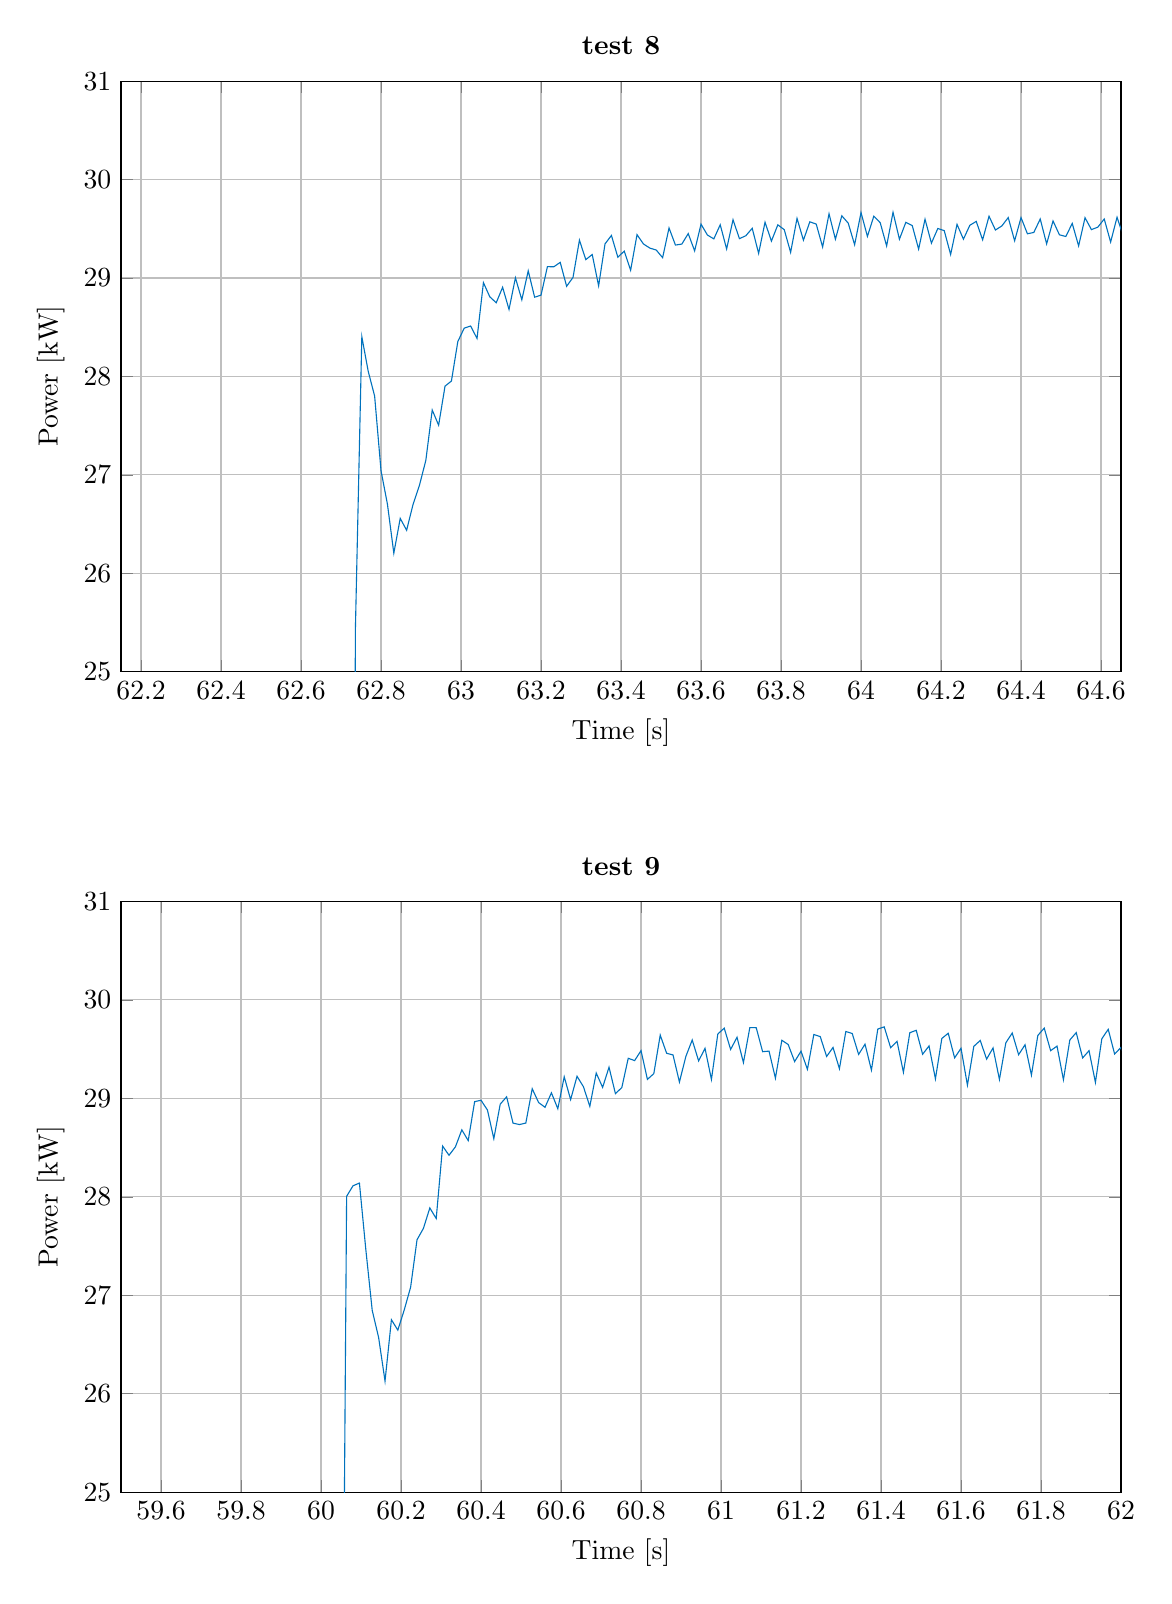
\begin{tikzpicture}

\begin{axis}[%
width=5in,
height=2.953in,
at={(1.142in,5.054in)},
scale only axis,
xmin=62.15,
xmax=64.65,
xlabel={Time [s]},
xmajorgrids,
ymin=25,
ymax=31,
ylabel={Power [kW]},
ymajorgrids,
axis background/.style={fill=white},
title style={font=\bfseries},
title={test 8}
]
\addplot [color=mycolor1,solid,forget plot]
  table[row sep=crcr]{%
62.7349371621339	24.4\\
62.736	25.4424576838972\\
62.752	28.4030812265324\\
62.768	28.0512974574802\\
62.784	27.8010409884802\\
62.8	27.0415707603226\\
62.816	26.7026546432169\\
62.832	26.2041597908499\\
62.848	26.5575942219516\\
62.864	26.4369945576032\\
62.88	26.6989089818192\\
62.896	26.8926754373254\\
62.912	27.1468354407678\\
62.928	27.6583831072402\\
62.944	27.5043271301642\\
62.96	27.900996439155\\
62.976	27.9527889501383\\
62.992	28.3541747320209\\
63.008	28.4907682174809\\
63.024	28.5120939933974\\
63.04	28.3856129052861\\
63.056	28.9524282511375\\
63.072	28.8081585184558\\
63.088	28.7483381809843\\
63.104	28.905481715845\\
63.12	28.6800866284995\\
63.136	29.0020205106714\\
63.152	28.7782866123935\\
63.168	29.0727341493215\\
63.184	28.8046589429982\\
63.2	28.8257888133401\\
63.216	29.1149239833679\\
63.232	29.1139417602266\\
63.248	29.1584718905294\\
63.264	28.9154164754809\\
63.28	29.006078349897\\
63.296	29.3836390854167\\
63.312	29.1864246414532\\
63.328	29.2383962976695\\
63.344	28.9202606806184\\
63.36	29.3463976952537\\
63.376	29.4319772305846\\
63.392	29.2112293404929\\
63.408	29.2725547680265\\
63.424	29.0785854051154\\
63.44	29.4400044201875\\
63.456	29.3455890829416\\
63.472	29.3036305583498\\
63.488	29.2837435864349\\
63.504	29.2063267344127\\
63.52	29.5079909499352\\
63.536	29.3345083090404\\
63.552	29.3441397916537\\
63.568	29.4508054083579\\
63.584	29.2752825781022\\
63.6	29.5467355838559\\
63.616	29.4360991514081\\
63.632	29.3969423492984\\
63.648	29.5406038475086\\
63.664	29.2943890831923\\
63.68	29.5917181960155\\
63.696	29.399432225\\
63.712	29.4290987431804\\
63.728	29.5045651393465\\
63.744	29.2499244511976\\
63.76	29.5662627353893\\
63.776	29.37473398179\\
63.792	29.5399700373706\\
63.808	29.4911540181884\\
63.824	29.2601683766641\\
63.84	29.6054356313395\\
63.856	29.3840322848672\\
63.872	29.5704600731767\\
63.888	29.5474422190815\\
63.904	29.3143258674411\\
63.92	29.6516569959687\\
63.936	29.393987742812\\
63.952	29.6317973517037\\
63.968	29.5569289358525\\
63.984	29.3377742993044\\
64	29.6642123877236\\
64.016	29.4221982121193\\
64.032	29.6282036290282\\
64.048	29.5612752385971\\
64.064	29.3254805251186\\
64.08	29.6674777366102\\
64.096	29.3936279518144\\
64.112	29.5652369029726\\
64.128	29.5330770714278\\
64.144	29.2930696807847\\
64.16	29.5968548728842\\
64.176	29.3539344983163\\
64.192	29.5026217067053\\
64.208	29.4807962803559\\
64.224	29.2386174288628\\
64.24	29.5445505920612\\
64.256	29.3944475160126\\
64.272	29.5350412847845\\
64.288	29.5747243212297\\
64.304	29.3878540308554\\
64.32	29.6273456065745\\
64.336	29.4873352828332\\
64.352	29.5284305671893\\
64.368	29.6135952328337\\
64.384	29.3777800198276\\
64.4	29.6136399523779\\
64.416	29.4488772583948\\
64.432	29.4626574004579\\
64.448	29.5991290350355\\
64.464	29.3463741268256\\
64.48	29.579615320415\\
64.496	29.4385026286765\\
64.512	29.421411664522\\
64.528	29.5541760571084\\
64.544	29.3261169549347\\
64.56	29.6118409642409\\
64.576	29.4914871023668\\
64.592	29.5160245810406\\
64.608	29.5992617394831\\
64.624	29.3650341613984\\
64.64	29.6163251518874\\
64.656	29.4217392121384\\
};
\end{axis}

\begin{axis}[%
width=5in,
height=2.953in,
at={(1.142in,0.952in)},
scale only axis,
xmin=59.5,
xmax=62,
xlabel={Time [s]},
xmajorgrids,
ymin=25,
ymax=31,
ylabel={Power [kW]},
ymajorgrids,
axis background/.style={fill=white},
title style={font=\bfseries},
title={test 9}
]
\addplot [color=mycolor1,solid,forget plot]
  table[row sep=crcr]{%
60.0574479456575	24.4\\
60.064	28.0053121291423\\
60.08	28.1119536476022\\
60.096	28.139654302488\\
60.112	27.4644747117544\\
60.128	26.8455948971027\\
60.144	26.5705374470559\\
60.16	26.1278736670319\\
60.176	26.7509422209034\\
60.192	26.6456186551507\\
60.208	26.8503038854632\\
60.224	27.082099430318\\
60.24	27.563638238526\\
60.256	27.6793031887683\\
60.272	27.8868317622428\\
60.288	27.7792436326451\\
60.304	28.5151353748245\\
60.32	28.4219643142107\\
60.336	28.5076319974809\\
60.352	28.68007265252\\
60.368	28.5712305881366\\
60.384	28.9668912894253\\
60.4	28.9805900884536\\
60.416	28.8827283439303\\
60.432	28.5905371777735\\
60.448	28.9413449052658\\
60.464	29.0158237368058\\
60.48	28.7485143167428\\
60.496	28.7340042993349\\
60.512	28.7491623125027\\
60.528	29.0978083640804\\
60.544	28.9573809307397\\
60.56	28.9095683218067\\
60.576	29.0563148935222\\
60.592	28.8948098067157\\
60.608	29.2191566768574\\
60.624	28.9874745477057\\
60.64	29.2244518854559\\
60.656	29.118550336913\\
60.672	28.9189278900851\\
60.688	29.2571261969677\\
60.704	29.1117948166092\\
60.72	29.3166446368119\\
60.736	29.0482353552077\\
60.752	29.1098569036696\\
60.768	29.4072803034994\\
60.784	29.38383806944\\
60.8	29.4847556799203\\
60.816	29.1928623475422\\
60.832	29.2516441679205\\
60.848	29.6427534192358\\
60.864	29.4581388137093\\
60.88	29.4410686266165\\
60.896	29.1659667179931\\
60.912	29.4253764741135\\
60.928	29.5930516827475\\
60.944	29.3809368300893\\
60.96	29.5076928154705\\
60.976	29.1922838405192\\
60.992	29.6543395459543\\
61.008	29.7130707290745\\
61.024	29.4973082187796\\
61.04	29.6207592956794\\
61.056	29.3628866793826\\
61.072	29.7190795906285\\
61.088	29.7178485767204\\
61.104	29.4742177186607\\
61.12	29.4802058664745\\
61.136	29.2050798910151\\
61.152	29.5907062023019\\
61.168	29.5466549089682\\
61.184	29.3739347478495\\
61.2	29.4790975028306\\
61.216	29.2949604491671\\
61.232	29.6486661336913\\
61.248	29.6278142923026\\
61.264	29.4257317785391\\
61.28	29.5173210663207\\
61.296	29.3016359871941\\
61.312	29.679485938853\\
61.328	29.6591128372316\\
61.344	29.446823902641\\
61.36	29.5507308532147\\
61.376	29.2871234151963\\
61.392	29.7048450886474\\
61.408	29.7262465286027\\
61.424	29.5150067061152\\
61.44	29.5795970625079\\
61.456	29.2651200566891\\
61.472	29.6670213325794\\
61.488	29.6914694357739\\
61.504	29.4480692451274\\
61.52	29.5326526756523\\
61.536	29.1982785689392\\
61.552	29.6082526906032\\
61.568	29.6615960155017\\
61.584	29.4110205670457\\
61.6	29.5086034219066\\
61.616	29.1342902047037\\
61.632	29.5287771626533\\
61.648	29.5881514989694\\
61.664	29.3989037016848\\
61.68	29.512144065463\\
61.696	29.1918956869594\\
61.712	29.5644980456455\\
61.728	29.6639789231395\\
61.744	29.4437590888439\\
61.76	29.5447387918769\\
61.776	29.2370232934586\\
61.792	29.6389490268731\\
61.808	29.7137196913698\\
61.824	29.484599699811\\
61.84	29.5311207829756\\
61.856	29.1894542045338\\
61.872	29.5932642013882\\
61.888	29.6678444040215\\
61.904	29.4106675641748\\
61.92	29.484428063441\\
61.936	29.1624155507597\\
61.952	29.6055983138457\\
61.968	29.7014276535192\\
61.984	29.4504382697124\\
62	29.5177564463993\\
62.016	29.2189524902785\\
};
\end{axis}
\end{tikzpicture}%
% \caption{Power disturbance on the output of the genset occuring from step of 10 to 30 kW load.}
% \label{fig:test8-9-10to30kwsteppower}
% \end{figure}

% \begin{figure}[H]
% \centering
% % This file was created by matlab2tikz.
%
%The latest updates can be retrieved from
%  http://www.mathworks.com/matlabcentral/fileexchange/22022-matlab2tikz-matlab2tikz
%where you can also make suggestions and rate matlab2tikz.
%
\definecolor{mycolor1}{rgb}{0.00000,0.44700,0.74100}%
%
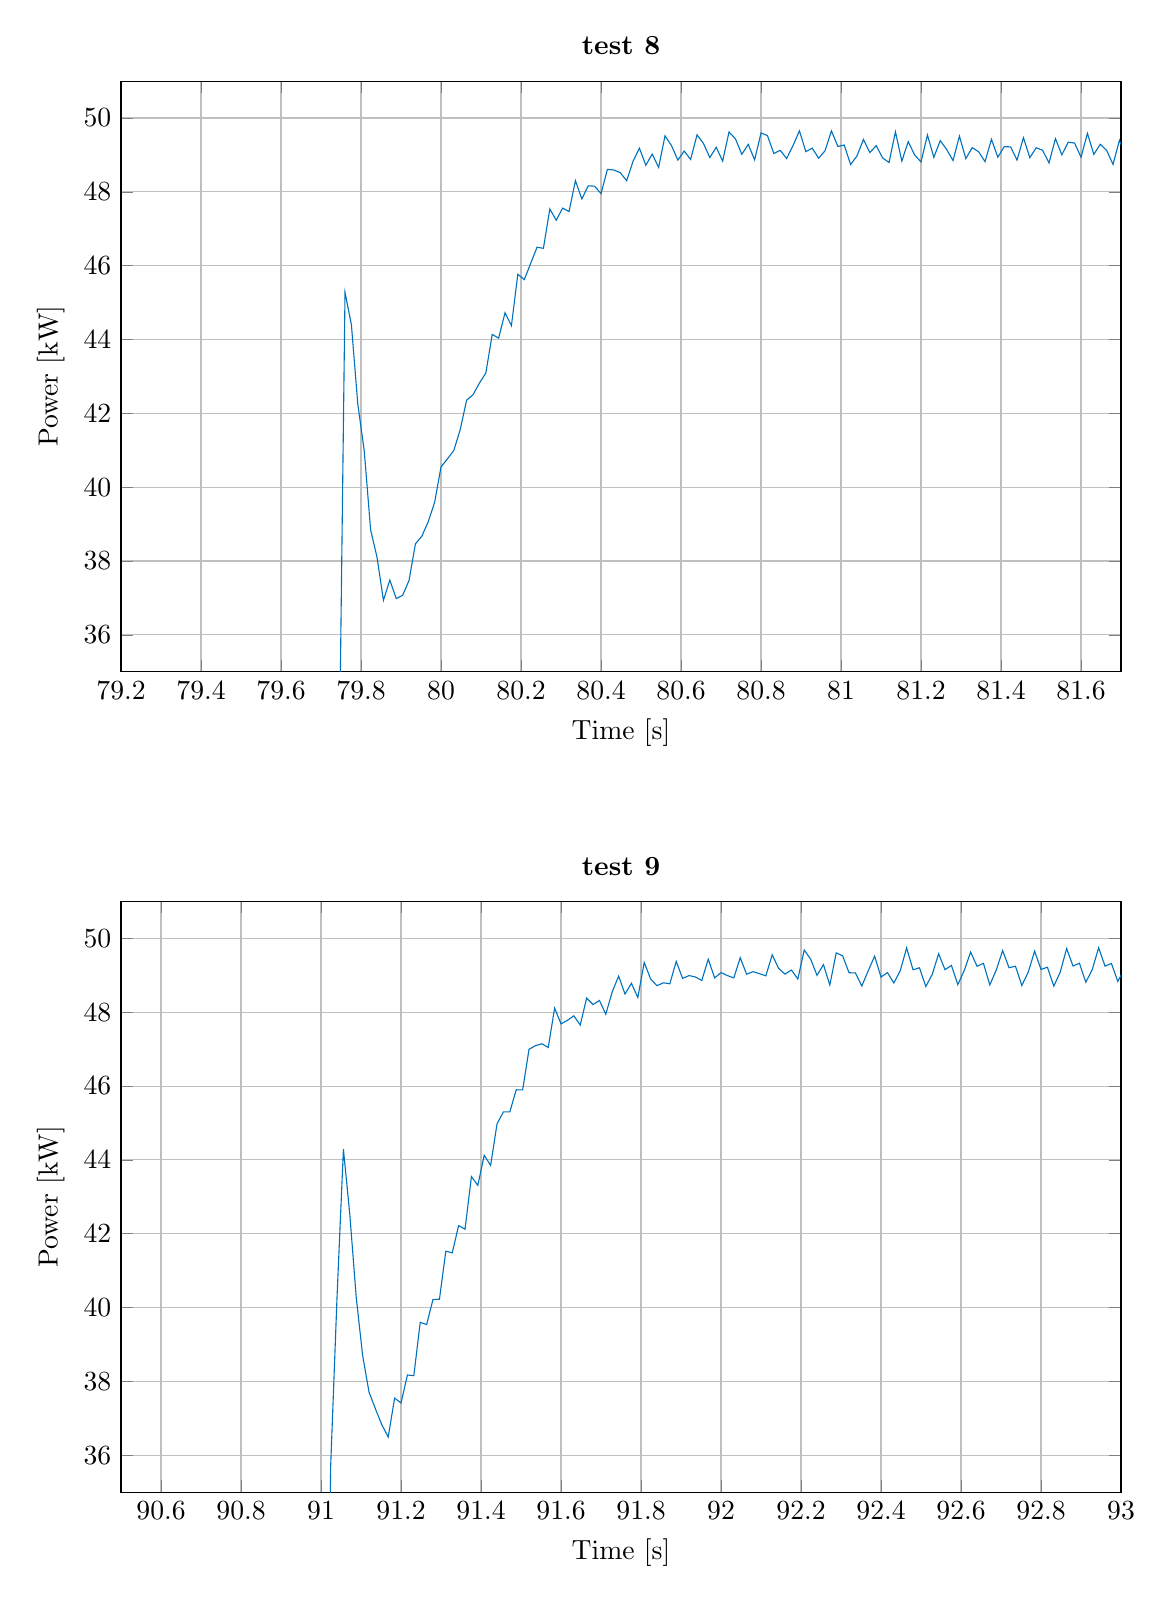
\begin{tikzpicture}

\begin{axis}[%
width=5in,
height=2.953in,
at={(1.142in,5.054in)},
scale only axis,
xmin=79.2,
xmax=81.7,
xlabel={Time [s]},
xmajorgrids,
ymin=35,
ymax=51,
ylabel={Power [kW]},
ymajorgrids,
axis background/.style={fill=white},
title style={font=\bfseries},
title={test 8}
]
\addplot [color=mycolor1,solid,forget plot]
  table[row sep=crcr]{%
79.7466206320365	33.4\\
79.76	45.2743640585935\\
79.776	44.3934694080188\\
79.792	42.2426168979348\\
79.808	40.9870018811951\\
79.824	38.8422828948872\\
79.84	38.0994944872162\\
79.856	36.9350725132218\\
79.872	37.4820777231701\\
79.888	36.9825994130418\\
79.904	37.0667117836692\\
79.92	37.4712443901036\\
79.936	38.4625024928484\\
79.952	38.6705352592546\\
79.968	39.0632014444107\\
79.984	39.5881484453769\\
80	40.5495482785925\\
80.016	40.7669849763984\\
80.032	40.9929285674189\\
80.048	41.5611292299107\\
80.064	42.3562284348487\\
80.08	42.5020160204764\\
80.096	42.8197886712259\\
80.112	43.0929501371591\\
80.128	44.1369826009975\\
80.144	44.0368675398091\\
80.16	44.7236351541416\\
80.176	44.3758867037075\\
80.192	45.7665322915113\\
80.208	45.6223379902661\\
80.224	46.0568213533774\\
80.24	46.4985476178232\\
80.256	46.4708068146594\\
80.272	47.5366481815678\\
80.288	47.230394526633\\
80.304	47.5590778862989\\
80.32	47.4659099408739\\
80.336	48.3022570346181\\
80.352	47.8060383990858\\
80.368	48.1632814966005\\
80.384	48.1534787174076\\
80.4	47.9505260531079\\
80.416	48.6099860673819\\
80.432	48.5909057798202\\
80.448	48.5208387017471\\
80.464	48.3031370889523\\
80.48	48.8244371643094\\
80.496	49.1828018807803\\
80.512	48.7192586960188\\
80.528	49.0235389829339\\
80.544	48.6614363797249\\
80.56	49.517867411849\\
80.576	49.2558166935807\\
80.592	48.8598635367213\\
80.608	49.1045422784807\\
80.624	48.8766257184439\\
80.64	49.5435274399768\\
80.656	49.312379903089\\
80.672	48.9291987277488\\
80.688	49.2065307380126\\
80.704	48.8329794796576\\
80.72	49.6208329640349\\
80.736	49.4360053202471\\
80.752	49.0164607029061\\
80.768	49.2844991602751\\
80.784	48.8669671391196\\
80.8	49.5957734161775\\
80.816	49.5247955937043\\
80.832	49.0389642328848\\
80.848	49.1235458066073\\
80.864	48.902661451523\\
80.88	49.253840432808\\
80.896	49.6523695684563\\
80.912	49.0893242972765\\
80.928	49.1847404598315\\
80.944	48.9103946944094\\
80.96	49.1118599679289\\
80.976	49.6513452094202\\
80.992	49.2310759024487\\
81.008	49.2671583371182\\
81.024	48.73853829712\\
81.04	48.9747424766801\\
81.056	49.4192692155636\\
81.072	49.0634293353339\\
81.088	49.251324283601\\
81.104	48.918656241811\\
81.12	48.7948480278641\\
81.136	49.6268796585319\\
81.152	48.8336843947131\\
81.168	49.3597495228428\\
81.184	48.9990071997576\\
81.2	48.8107353129842\\
81.216	49.5398572475844\\
81.232	48.9342050590027\\
81.248	49.3886919094541\\
81.264	49.1477412487965\\
81.28	48.8481562279965\\
81.296	49.5095056216094\\
81.312	48.8996206865821\\
81.328	49.1986955218005\\
81.344	49.0866023365198\\
81.36	48.8176280640413\\
81.376	49.4242788320324\\
81.392	48.9381305575258\\
81.408	49.2247845360366\\
81.424	49.2184484917353\\
81.44	48.8596507896001\\
81.456	49.4673711374916\\
81.472	48.9266288506245\\
81.488	49.1946577966766\\
81.504	49.1252321277427\\
81.52	48.7825132778131\\
81.536	49.4416243529283\\
81.552	49.0033343072342\\
81.568	49.3456865909196\\
81.584	49.3212614837959\\
81.6	48.938100432362\\
81.616	49.5851867403416\\
81.632	49.0141945275597\\
81.648	49.2891060387813\\
81.664	49.1231408757666\\
81.68	48.7434017437153\\
81.696	49.3951857840362\\
81.712	48.9739456606087\\
};
\end{axis}

\begin{axis}[%
width=5in,
height=2.953in,
at={(1.142in,0.952in)},
scale only axis,
xmin=90.5,
xmax=93,
xlabel={Time [s]},
xmajorgrids,
ymin=35,
ymax=51,
ylabel={Power [kW]},
ymajorgrids,
axis background/.style={fill=white},
title style={font=\bfseries},
title={test 9}
]
\addplot [color=mycolor1,solid,forget plot]
  table[row sep=crcr]{%
91.021794760337	33.4\\
91.024	35.6709087570807\\
91.04	40.2781194465096\\
91.056	44.2890954553868\\
91.072	42.5168695355984\\
91.088	40.2754982705915\\
91.104	38.7027477709053\\
91.12	37.7091953336589\\
91.136	37.2554385487108\\
91.152	36.8241724093697\\
91.168	36.4925050315707\\
91.184	37.5466894323198\\
91.2	37.413865516009\\
91.216	38.1721693929602\\
91.232	38.1544532722348\\
91.248	39.5980229916109\\
91.264	39.5407336914697\\
91.28	40.2204180579232\\
91.296	40.2242086597046\\
91.312	41.5271953461624\\
91.328	41.4809503242433\\
91.344	42.2199222530034\\
91.36	42.1231900411933\\
91.376	43.5461578500464\\
91.392	43.3089069468841\\
91.408	44.1249145653788\\
91.424	43.8516920048469\\
91.44	44.9743727294785\\
91.456	45.3019672259098\\
91.472	45.2999654953558\\
91.488	45.899209574146\\
91.504	45.8952915481544\\
91.52	46.9941913830487\\
91.536	47.0945741537896\\
91.552	47.1464825380522\\
91.568	47.0445873737489\\
91.584	48.1120542496079\\
91.6	47.685315958879\\
91.616	47.7801546362221\\
91.632	47.9031086606709\\
91.648	47.6540391461223\\
91.664	48.3817232340378\\
91.68	48.20912696512\\
91.696	48.3181601176492\\
91.712	47.9472173172413\\
91.728	48.5532041438508\\
91.744	48.9792842514156\\
91.76	48.4932256476553\\
91.776	48.7839035104386\\
91.792	48.3996903254185\\
91.808	49.3489055528521\\
91.824	48.9013557394647\\
91.84	48.7197206196792\\
91.856	48.798224145428\\
91.872	48.770690766448\\
91.888	49.3765317462585\\
91.904	48.9152279770916\\
91.92	48.9938016630102\\
91.936	48.9548556631577\\
91.952	48.8615033905653\\
91.968	49.436450941825\\
91.984	48.9306021331172\\
92	49.0753213399429\\
92.016	48.9935118858675\\
92.032	48.9304030535534\\
92.048	49.4772029719594\\
92.064	49.0300391683276\\
92.08	49.099081130677\\
92.096	49.0456321682215\\
92.112	48.9864883158197\\
92.128	49.5563005892848\\
92.144	49.1875887376944\\
92.16	49.0335141652823\\
92.176	49.1442184799801\\
92.192	48.8998660230576\\
92.208	49.6849782314763\\
92.224	49.440108106854\\
92.24	48.998807469394\\
92.256	49.2900020380559\\
92.272	48.7385278896083\\
92.288	49.6078962183094\\
92.304	49.5295459748347\\
92.32	49.0706196732594\\
92.336	49.0637991417848\\
92.352	48.7109508377294\\
92.368	49.1216518090669\\
92.384	49.5184565279308\\
92.4	48.9518510310115\\
92.416	49.0746832178632\\
92.432	48.7932974888919\\
92.448	49.1224941336088\\
92.464	49.7422139894827\\
92.48	49.1500286513089\\
92.496	49.204477722146\\
92.512	48.6964744125092\\
92.528	49.0255349570117\\
92.544	49.5838766452116\\
92.56	49.1519588020696\\
92.576	49.2691838980146\\
92.592	48.749637902525\\
92.608	49.1300766147348\\
92.624	49.6310379282381\\
92.64	49.2460816144552\\
92.656	49.3254577395908\\
92.672	48.7409301948663\\
92.688	49.1408756729875\\
92.704	49.6700098033573\\
92.72	49.2068282508305\\
92.736	49.2458390386689\\
92.752	48.7246946261058\\
92.768	49.0866393647319\\
92.784	49.6551382341736\\
92.8	49.1586805631763\\
92.816	49.2196493797743\\
92.832	48.7061392857316\\
92.848	49.0860966678099\\
92.864	49.7253638716565\\
92.88	49.2527611706095\\
92.896	49.3284920411758\\
92.912	48.8140661244379\\
92.928	49.1512032042904\\
92.944	49.7482173170621\\
92.96	49.249342379859\\
92.976	49.3222097674592\\
92.992	48.8355795099588\\
93.008	49.1643743594377\\
};
\end{axis}
\end{tikzpicture}%
% \caption{Power disturbance on the output of the genset occuring from step of 10 to 50 kW load.}
% \label{fig:test8-9-10to50kwsteppower}
% \end{figure}

% \begin{figure}[H]
% \centering
% % This file was created by matlab2tikz.
%
%The latest updates can be retrieved from
%  http://www.mathworks.com/matlabcentral/fileexchange/22022-matlab2tikz-matlab2tikz
%where you can also make suggestions and rate matlab2tikz.
%
\definecolor{mycolor1}{rgb}{0.00000,0.44700,0.74100}%
%
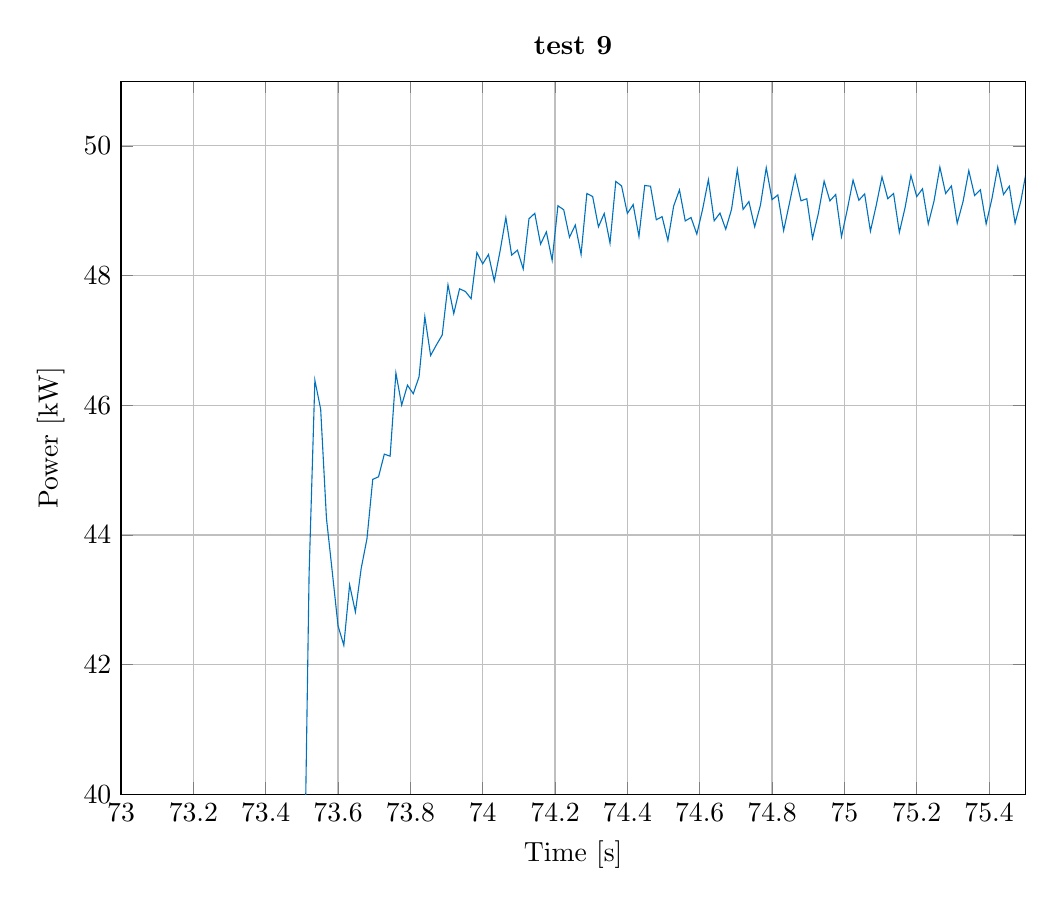
\begin{tikzpicture}

\begin{axis}[%
width=4.521in,
height=3.566in,
at={(0.758in,0.481in)},
scale only axis,
xmin=73,
xmax=75.5,
xlabel={Time [s]},
xmajorgrids,
ymin=40,
ymax=51,
ylabel={Power [kW]},
ymajorgrids,
axis background/.style={fill=white},
title style={font=\bfseries},
title={test 9}
]
\addplot [color=mycolor1,solid,forget plot]
  table[row sep=crcr]{%
73.5078621497172	38.9\\
73.52	43.4031447990291\\
73.536	46.3842248073813\\
73.552	45.9395391511731\\
73.568	44.2566449153382\\
73.584	43.4352837869724\\
73.6	42.5990610354096\\
73.616	42.2981371881454\\
73.632	43.2314864985936\\
73.648	42.8135813247251\\
73.664	43.4831119758994\\
73.68	43.9421782371148\\
73.696	44.8575329417421\\
73.712	44.8975653289114\\
73.728	45.246889079378\\
73.744	45.2148422180836\\
73.76	46.4984866684654\\
73.776	46.0028516744185\\
73.792	46.3105825836809\\
73.808	46.1784565987382\\
73.824	46.4394215190833\\
73.84	47.3663273063149\\
73.856	46.7686348105219\\
73.872	46.9308850235067\\
73.888	47.0830317703059\\
73.904	47.8576839667287\\
73.92	47.4149020711183\\
73.936	47.7966774972287\\
73.952	47.7563540198693\\
73.968	47.6440269679527\\
73.984	48.3553821701992\\
74	48.1818158102376\\
74.016	48.325317449687\\
74.032	47.9179403093051\\
74.048	48.3785011833575\\
74.064	48.8956999155652\\
74.08	48.3162235472615\\
74.096	48.3920532583084\\
74.112	48.1035533054126\\
74.128	48.8775198652501\\
74.144	48.9606610639663\\
74.16	48.4855792336681\\
74.176	48.6742507885375\\
74.192	48.2352740426307\\
74.208	49.0774389636622\\
74.224	49.0156539240636\\
74.24	48.5920492410111\\
74.256	48.780557469661\\
74.272	48.3279895620684\\
74.288	49.2666308375377\\
74.304	49.2201467777135\\
74.32	48.7518829802954\\
74.336	48.9582582926528\\
74.352	48.5013606093014\\
74.368	49.4530187706747\\
74.384	49.3826453078175\\
74.4	48.9592094526832\\
74.416	49.095092494218\\
74.432	48.6035992906148\\
74.448	49.390146086557\\
74.464	49.3785609406076\\
74.48	48.8617369604711\\
74.496	48.9091927255981\\
74.512	48.5415305511437\\
74.528	49.0738416303755\\
74.544	49.3215851743142\\
74.56	48.8437824979766\\
74.576	48.8961788460477\\
74.592	48.6396916650296\\
74.608	49.0230644835874\\
74.624	49.479236010302\\
74.64	48.8450256649736\\
74.656	48.964572266485\\
74.672	48.7155763234493\\
74.688	49.0222913622601\\
74.704	49.6346407796616\\
74.72	49.021103614694\\
74.736	49.1422629292319\\
74.752	48.752616313942\\
74.768	49.0891287326328\\
74.784	49.6642510765979\\
74.8	49.172038379269\\
74.816	49.2439668531784\\
74.832	48.6944350148374\\
74.848	49.1131827135957\\
74.864	49.5442050503397\\
74.88	49.153644429487\\
74.896	49.1856531080146\\
74.912	48.5761401807526\\
74.928	48.9575463052103\\
74.944	49.457020531958\\
74.96	49.1528203561873\\
74.976	49.2514801834472\\
74.992	48.601555883771\\
75.008	49.0176991938654\\
75.024	49.4728281421887\\
75.04	49.1618799586601\\
75.056	49.259933618062\\
75.072	48.684682050478\\
75.088	49.0831181109114\\
75.104	49.5222584389752\\
75.12	49.1862938270968\\
75.136	49.2660869592126\\
75.152	48.6670599225678\\
75.168	49.0547336130764\\
75.184	49.5451496141178\\
75.2	49.219268380291\\
75.216	49.3386579902501\\
75.232	48.7962379865704\\
75.248	49.1550177815162\\
75.264	49.6733464060076\\
75.28	49.2669336382836\\
75.296	49.3833208671832\\
75.312	48.8079210253473\\
75.328	49.140362557875\\
75.344	49.6183368155404\\
75.36	49.236021090328\\
75.376	49.3225728376753\\
75.392	48.79711428851\\
75.408	49.188745833938\\
75.424	49.6742988131322\\
75.44	49.2516379306024\\
75.456	49.378987167022\\
75.472	48.8090349207297\\
75.488	49.152209429876\\
75.504	49.6383840351801\\
};
\end{axis}
\end{tikzpicture}%
% \caption{Power disturbance on the output of the genset occuring from step of 30 to 50 kW load.}
% \label{fig:test9-30to50kwsteppower}
% \end{figure}

% \begin{figure}[H]
% \centering
% % This file was created by matlab2tikz.
%
%The latest updates can be retrieved from
%  http://www.mathworks.com/matlabcentral/fileexchange/22022-matlab2tikz-matlab2tikz
%where you can also make suggestions and rate matlab2tikz.
%
\definecolor{mycolor1}{rgb}{0.00000,0.44700,0.74100}%
%
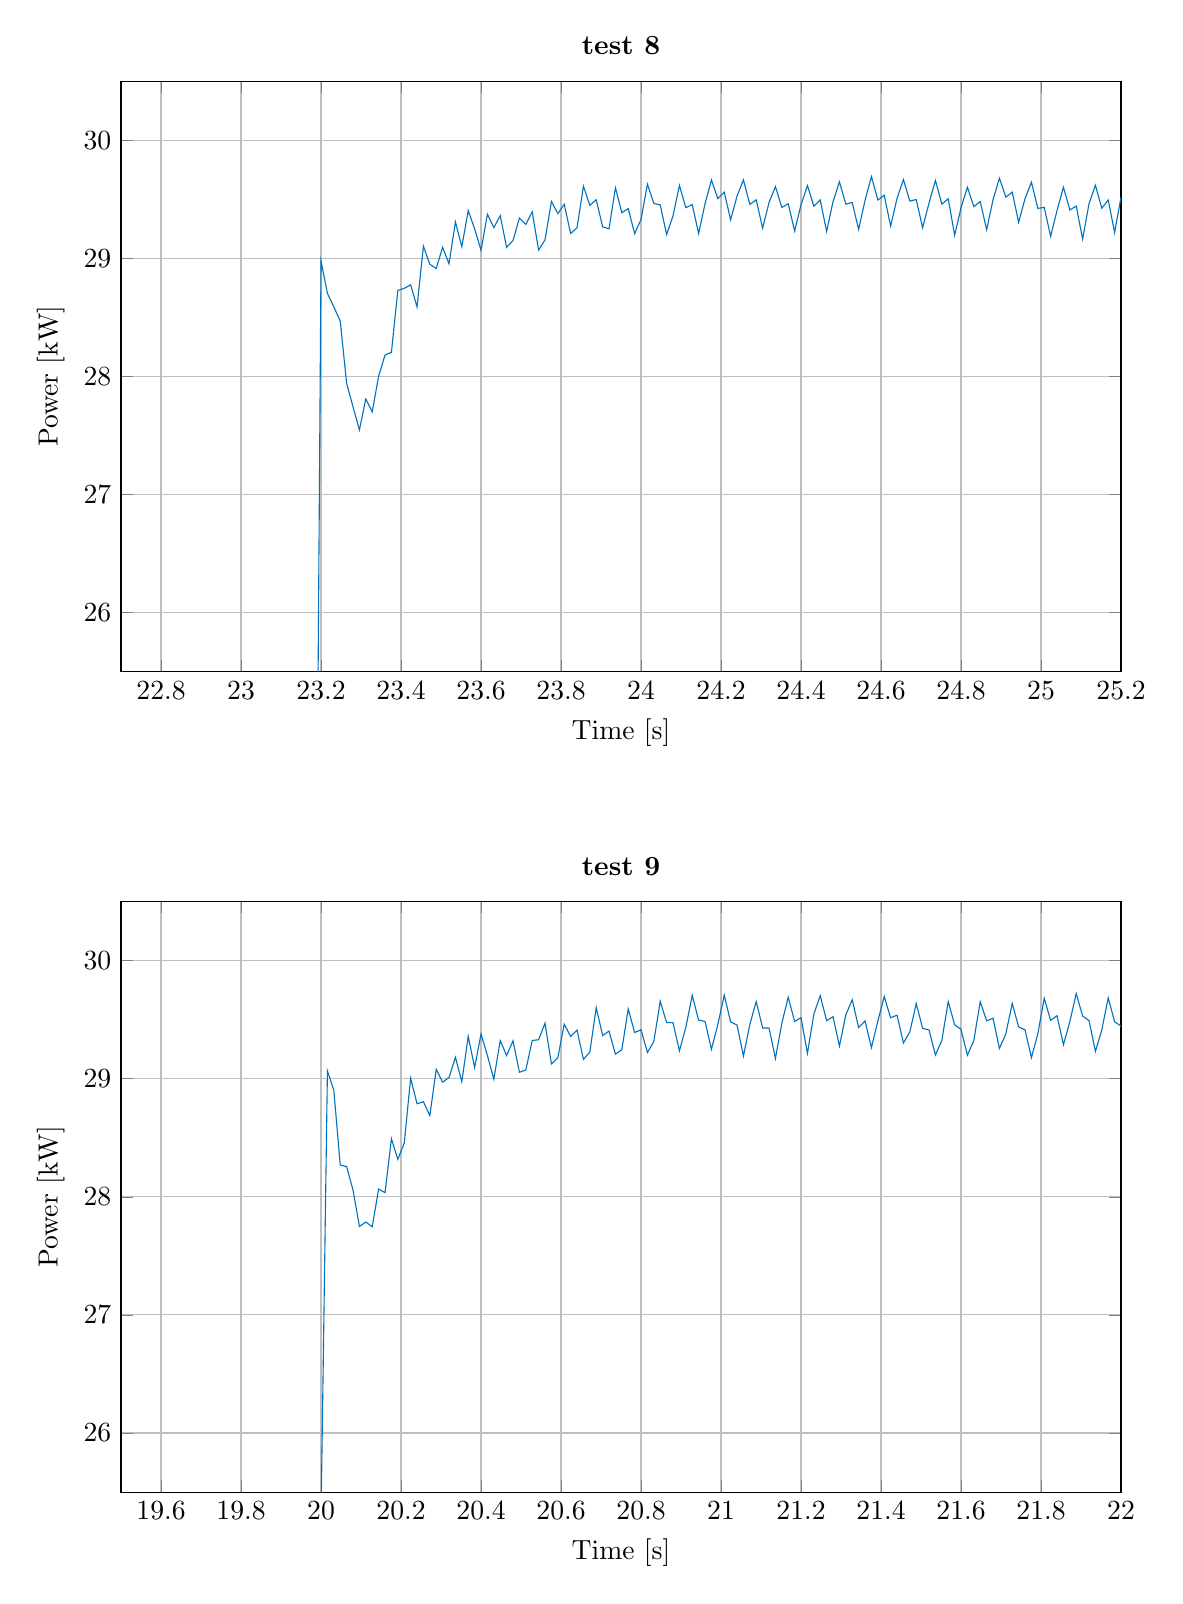
\begin{tikzpicture}

\begin{axis}[%
width=5in,
height=2.953in,
at={(1.142in,5.054in)},
scale only axis,
xmin=22.7,
xmax=25.2,
xlabel={Time [s]},
xmajorgrids,
ymin=25.5,
ymax=30.5,
ylabel={Power [kW]},
ymajorgrids,
axis background/.style={fill=white},
title style={font=\bfseries},
title={test 8}
]
\addplot [color=mycolor1,solid,forget plot]
  table[row sep=crcr]{%
23.1916827247994	25\\
23.2	28.9761812280174\\
23.216	28.7034278635087\\
23.232	28.5879460551656\\
23.248	28.4689722606493\\
23.264	27.9422153243289\\
23.28	27.74196239121\\
23.296	27.5475518431057\\
23.312	27.8094526619361\\
23.328	27.700451078608\\
23.344	28.0021873474322\\
23.36	28.1808232239084\\
23.376	28.2051026394195\\
23.392	28.7277446770833\\
23.408	28.7452680232531\\
23.424	28.7755464588241\\
23.44	28.5881047495842\\
23.456	29.1021845964438\\
23.472	28.9497847837278\\
23.488	28.9135475878345\\
23.504	29.0930110020825\\
23.52	28.9534582222064\\
23.536	29.3074396419981\\
23.552	29.0977608738619\\
23.568	29.4035225066672\\
23.584	29.2497786733592\\
23.6	29.0681985504099\\
23.616	29.3735896485135\\
23.632	29.2599496412232\\
23.648	29.3611252693687\\
23.664	29.0924857432147\\
23.68	29.1502677533941\\
23.696	29.340864523982\\
23.712	29.2872040180088\\
23.728	29.3931148406819\\
23.744	29.0691069343713\\
23.76	29.156643460951\\
23.776	29.4811143805685\\
23.792	29.37827020368\\
23.808	29.4571453035838\\
23.824	29.2101074478716\\
23.84	29.2572389570849\\
23.856	29.6100636459803\\
23.872	29.4481465300031\\
23.888	29.4958172091512\\
23.904	29.2663091073369\\
23.92	29.2493906245267\\
23.936	29.5971101065909\\
23.952	29.3857721142585\\
23.968	29.4215450533514\\
23.984	29.2086116270507\\
24	29.328170239195\\
24.016	29.627315872157\\
24.032	29.4640791462457\\
24.048	29.4519030432502\\
24.064	29.2013285919211\\
24.08	29.3597309312137\\
24.096	29.6173736433362\\
24.112	29.4283947035307\\
24.128	29.4549720998017\\
24.144	29.2098043042457\\
24.16	29.4610402018116\\
24.176	29.6626361915609\\
24.192	29.5046951199298\\
24.208	29.5605709195911\\
24.224	29.3253326991344\\
24.24	29.5257523517466\\
24.256	29.6634959849433\\
24.272	29.4559710076124\\
24.288	29.494564036522\\
24.304	29.2548280353941\\
24.32	29.4725092890054\\
24.336	29.606714253325\\
24.352	29.4302103710441\\
24.368	29.4618787105569\\
24.384	29.2312031997243\\
24.4	29.4537569858665\\
24.416	29.6162033258584\\
24.432	29.4405651754057\\
24.448	29.4944422738692\\
24.464	29.2268600760824\\
24.48	29.4790852412078\\
24.496	29.6472091335788\\
24.512	29.4587329742119\\
24.528	29.4726123541534\\
24.544	29.2441559635418\\
24.56	29.4897672421324\\
24.576	29.6911878997582\\
24.592	29.4935302483806\\
24.608	29.5332937429689\\
24.624	29.2722242436429\\
24.64	29.5067204631821\\
24.656	29.666511031211\\
24.672	29.4842861894421\\
24.688	29.4975155179796\\
24.704	29.2584262901394\\
24.72	29.4676441596279\\
24.736	29.6587750065477\\
24.752	29.4584550046005\\
24.768	29.5036152189178\\
24.784	29.1947652175148\\
24.8	29.428026963411\\
24.816	29.6013256429514\\
24.832	29.4378624674673\\
24.848	29.4801727953723\\
24.864	29.2416533362681\\
24.88	29.4949158551085\\
24.896	29.6789031651815\\
24.912	29.5178929519904\\
24.928	29.5604351846232\\
24.944	29.3049745763599\\
24.96	29.5042702596805\\
24.976	29.6446709765497\\
24.992	29.4223884693646\\
25.008	29.4308900176188\\
25.024	29.1860016621515\\
25.04	29.4043502792146\\
25.056	29.6018221733937\\
25.072	29.4095182670484\\
25.088	29.4420319579254\\
25.104	29.1619034743373\\
25.12	29.4625624513762\\
25.136	29.6184955178272\\
25.152	29.4228758258205\\
25.168	29.4935733607827\\
25.184	29.2179489328206\\
25.2	29.5186517832885\\
25.2	29.5186517832885\\
};
\end{axis}

\begin{axis}[%
width=5in,
height=2.953in,
at={(1.142in,0.952in)},
scale only axis,
xmin=19.5,
xmax=22,
xlabel={Time [s]},
xmajorgrids,
ymin=25.5,
ymax=30.5,
ylabel={Power [kW]},
ymajorgrids,
axis background/.style={fill=white},
title style={font=\bfseries},
title={test 9}
]
\addplot [color=mycolor1,solid,forget plot]
  table[row sep=crcr]{%
20	25.281738771017\\
20.016	29.0659190572832\\
20.032	28.9004919507762\\
20.048	28.2694997724295\\
20.064	28.2562412659055\\
20.08	28.0568266012932\\
20.096	27.7493068003828\\
20.112	27.7862007294398\\
20.128	27.7459948605958\\
20.144	28.0656140830703\\
20.16	28.0350766543516\\
20.176	28.4909764684018\\
20.192	28.3171803366919\\
20.208	28.4542483828152\\
20.224	29.003236426465\\
20.24	28.7880793528529\\
20.256	28.8049783345782\\
20.272	28.6869542065433\\
20.288	29.0789395412715\\
20.304	28.9697590899987\\
20.32	29.0102099271242\\
20.336	29.1808558453904\\
20.352	28.97411725732\\
20.368	29.359048270105\\
20.384	29.0946285047516\\
20.4	29.3783900063533\\
20.416	29.1967036576009\\
20.432	28.9951094718122\\
20.448	29.3230615442837\\
20.464	29.1956331432741\\
20.48	29.321019502214\\
20.496	29.0543674168753\\
20.512	29.0740753169138\\
20.528	29.3234199017003\\
20.544	29.3297863307067\\
20.56	29.4700647678764\\
20.576	29.1241505704278\\
20.592	29.1758585257745\\
20.608	29.4614386139367\\
20.624	29.3577572811228\\
20.64	29.4112744709178\\
20.656	29.1635401773564\\
20.672	29.2253448471353\\
20.688	29.6017274559061\\
20.704	29.3660571726517\\
20.72	29.4027470473163\\
20.736	29.2074681137843\\
20.752	29.2452131982447\\
20.768	29.5906251798363\\
20.784	29.3917842865582\\
20.8	29.4134752328405\\
20.816	29.2217281522022\\
20.832	29.3148196565072\\
20.848	29.6562109660622\\
20.864	29.4744088470325\\
20.88	29.4742179354122\\
20.896	29.2356657280041\\
20.912	29.434934888061\\
20.928	29.7051235679176\\
20.944	29.4963687602772\\
20.96	29.4846932494865\\
20.976	29.248612277845\\
20.992	29.4579606774929\\
21.008	29.7070973197171\\
21.024	29.4809668798537\\
21.04	29.4540715298829\\
21.056	29.1919330285217\\
21.072	29.4589116458453\\
21.088	29.653407289022\\
21.104	29.4293886142608\\
21.12	29.42881201719\\
21.136	29.1713986476534\\
21.152	29.4684808250572\\
21.168	29.6896887338005\\
21.184	29.4844193766\\
21.2	29.5166424813642\\
21.216	29.2137963549068\\
21.232	29.5457262162831\\
21.248	29.7027784757262\\
21.264	29.4909108040929\\
21.28	29.5249344859394\\
21.296	29.2761738447562\\
21.312	29.5402875162426\\
21.328	29.6682970104379\\
21.344	29.4330388272392\\
21.36	29.4888530357118\\
21.376	29.2628260115736\\
21.392	29.4871379039859\\
21.408	29.6957459957548\\
21.424	29.5163145912019\\
21.44	29.5371039092056\\
21.456	29.302484770226\\
21.472	29.3954470904006\\
21.488	29.6358003277697\\
21.504	29.426516085221\\
21.52	29.4118719935113\\
21.536	29.2003525870132\\
21.552	29.3236989166107\\
21.568	29.6517680547304\\
21.584	29.4570533877079\\
21.6	29.4172270442249\\
21.616	29.1994511736129\\
21.632	29.3227417202854\\
21.648	29.6523609781355\\
21.664	29.4897574139711\\
21.68	29.5115588506655\\
21.696	29.2560977411667\\
21.712	29.3790994385165\\
21.728	29.6375986689143\\
21.744	29.4381952986168\\
21.76	29.4139689929173\\
21.776	29.1777602835137\\
21.792	29.3803461096417\\
21.808	29.6807740615429\\
21.824	29.4938249750955\\
21.84	29.5334019217926\\
21.856	29.2870896432577\\
21.872	29.4826843987727\\
21.888	29.7210757273362\\
21.904	29.5301965634193\\
21.92	29.4911431679326\\
21.936	29.2315591415346\\
21.952	29.4147301834832\\
21.968	29.6838590621859\\
21.984	29.4809549219531\\
22	29.4465453331174\\
22.016	29.2027923944449\\
};
\end{axis}
\end{tikzpicture}%
% \caption{Power disturbance on the output of the genset occuring from step of 20 to 30 kW load.}
% \label{fig:test8-9-20to30kwsteppower}
% \end{figure}

% \begin{figure}[H]
% \centering
% % This file was created by matlab2tikz.
%
%The latest updates can be retrieved from
%  http://www.mathworks.com/matlabcentral/fileexchange/22022-matlab2tikz-matlab2tikz
%where you can also make suggestions and rate matlab2tikz.
%
\definecolor{mycolor1}{rgb}{0.00000,0.44700,0.74100}%
%
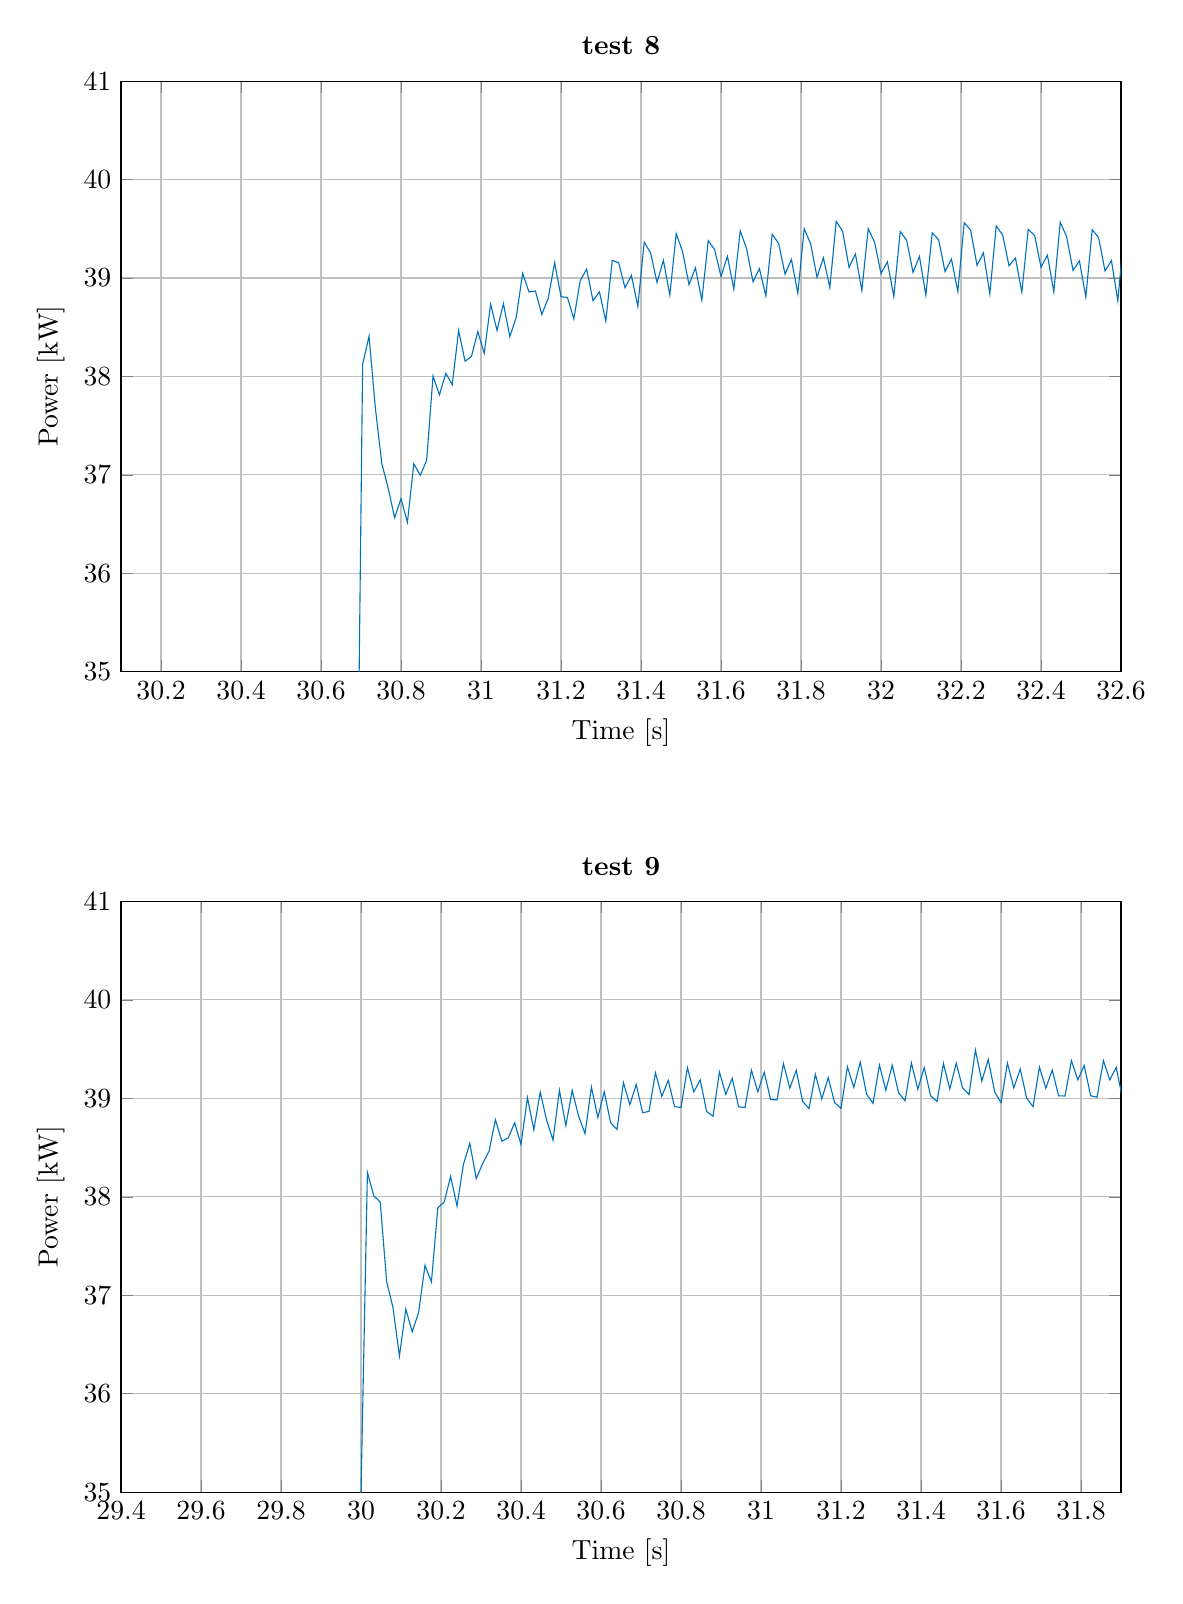
\begin{tikzpicture}

\begin{axis}[%
width=5in,
height=2.953in,
at={(1.142in,5.054in)},
scale only axis,
xmin=30.1,
xmax=32.6,
xlabel={Time [s]},
xmajorgrids,
ymin=35,
ymax=41,
ylabel={Power [kW]},
ymajorgrids,
axis background/.style={fill=white},
title style={font=\bfseries},
title={test 8}
]
\addplot [color=mycolor1,solid,forget plot]
  table[row sep=crcr]{%
30.6936811682031	34.4\\
30.704	38.1220285620402\\
30.72	38.4088835912484\\
30.736	37.6727688725507\\
30.752	37.1132800226009\\
30.768	36.8634335805264\\
30.784	36.5653588063833\\
30.8	36.7575995830564\\
30.816	36.5175281165323\\
30.832	37.1127566713377\\
30.848	36.9951916911949\\
30.864	37.146143340967\\
30.88	38.0038043740518\\
30.896	37.812353248168\\
30.912	38.0308609375993\\
30.928	37.9146546811912\\
30.944	38.4653558517458\\
30.96	38.154581950345\\
30.976	38.2017823942871\\
30.992	38.4559762206029\\
31.008	38.2338806623908\\
31.024	38.7342292262225\\
31.04	38.4672931595979\\
31.056	38.739444184513\\
31.072	38.4034971944473\\
31.088	38.5992684979664\\
31.104	39.046570279834\\
31.12	38.8575720821428\\
31.136	38.8675835569183\\
31.152	38.6295397416272\\
31.168	38.7946227462433\\
31.184	39.1543944725754\\
31.2	38.8101103737152\\
31.216	38.8009567471922\\
31.232	38.584347801451\\
31.248	38.9723429528036\\
31.264	39.090942559004\\
31.28	38.7693349337707\\
31.296	38.8590551606917\\
31.312	38.5619946240107\\
31.328	39.1777527463532\\
31.344	39.1553385303522\\
31.36	38.9001402405042\\
31.376	39.0249122057352\\
31.392	38.7111688779087\\
31.408	39.3650285266821\\
31.424	39.2524509629077\\
31.44	38.9547136692704\\
31.456	39.1783885515091\\
31.472	38.8262945997279\\
31.488	39.4499481515828\\
31.504	39.2650454261117\\
31.52	38.9327192855002\\
31.536	39.1023273577299\\
31.552	38.7735064236951\\
31.568	39.3791357994247\\
31.584	39.288758482838\\
31.6	39.0148402326884\\
31.616	39.2202702489604\\
31.632	38.887032364547\\
31.648	39.4796482919537\\
31.664	39.2963660247172\\
31.68	38.9610013726176\\
31.696	39.0948419403629\\
31.712	38.8188284049458\\
31.728	39.4444427542085\\
31.744	39.3503517596198\\
31.76	39.0389930826964\\
31.776	39.1874946195829\\
31.792	38.8442451523174\\
31.808	39.5000489944146\\
31.824	39.3477200570998\\
31.84	39.0079006271946\\
31.856	39.2042263873675\\
31.872	38.9032072261867\\
31.888	39.5751222117921\\
31.904	39.4746545579479\\
31.92	39.1081958498781\\
31.936	39.2428182968856\\
31.952	38.8733946850385\\
31.968	39.5011020342526\\
31.984	39.3609899422205\\
32	39.0451980302526\\
32.016	39.1632046184308\\
32.032	38.8118232571152\\
32.048	39.4718399843816\\
32.064	39.38367237625\\
32.08	39.056442910818\\
32.096	39.2195689818693\\
32.112	38.8258404429622\\
32.128	39.4573455879424\\
32.144	39.3885015545951\\
32.16	39.0652761667864\\
32.176	39.1929097296981\\
32.192	38.8625798164391\\
32.208	39.5607235276013\\
32.224	39.4868809046263\\
32.24	39.1278541658036\\
32.256	39.2554381161375\\
32.272	38.8394573053181\\
32.288	39.5291121471239\\
32.304	39.436295070895\\
32.32	39.123823442348\\
32.336	39.2025253237886\\
32.352	38.8566490122056\\
32.368	39.4924135910256\\
32.384	39.4322435849582\\
32.4	39.1089022140225\\
32.416	39.232096047738\\
32.432	38.8587450738041\\
32.448	39.5673701535025\\
32.464	39.4199326362811\\
32.48	39.0770415432101\\
32.496	39.1726708480794\\
32.512	38.8075226000662\\
32.528	39.4907162671158\\
32.544	39.4087870033041\\
32.56	39.0715167300747\\
32.576	39.175260598153\\
32.592	38.7696261199989\\
32.608	39.4703861216346\\
};
\end{axis}

\begin{axis}[%
width=5in,
height=2.953in,
at={(1.142in,0.952in)},
scale only axis,
xmin=29.4,
xmax=31.9,
xlabel={Time [s]},
xmajorgrids,
ymin=35,
ymax=41,
ylabel={Power [kW]},
ymajorgrids,
axis background/.style={fill=white},
title style={font=\bfseries},
title={test 9}
]
\addplot [color=mycolor1,solid,forget plot]
  table[row sep=crcr]{%
29.998256869187	34.4\\
30	35.0027792568644\\
30.016	38.2477268980784\\
30.032	38.009386339557\\
30.048	37.9465814788326\\
30.064	37.1408785086478\\
30.08	36.8727122903534\\
30.096	36.3821655295922\\
30.112	36.8596051913343\\
30.128	36.6280532007832\\
30.144	36.8255992877574\\
30.16	37.3033887675506\\
30.176	37.1360304936205\\
30.192	37.8875314059043\\
30.208	37.9475482926332\\
30.224	38.2064108295261\\
30.24	37.9063424233036\\
30.256	38.3293595461292\\
30.272	38.5440298945629\\
30.288	38.1847446742017\\
30.304	38.3374072517654\\
30.32	38.4627867279623\\
30.336	38.7831415996197\\
30.352	38.5656817861405\\
30.368	38.598391500922\\
30.384	38.7516681376571\\
30.4	38.5326345782116\\
30.416	39.0069606040768\\
30.432	38.6814724218739\\
30.448	39.0627235376108\\
30.464	38.778283667058\\
30.48	38.5758981034426\\
30.496	39.0821980037281\\
30.512	38.7234576144511\\
30.528	39.0807812988907\\
30.544	38.8185770540135\\
30.56	38.6426204508291\\
30.576	39.1152026884546\\
30.592	38.8047155041769\\
30.608	39.0673673887768\\
30.624	38.7521439304432\\
30.64	38.6845100888744\\
30.656	39.1601662388308\\
30.672	38.935287914218\\
30.688	39.1406391703425\\
30.704	38.8543558556124\\
30.72	38.8673887399195\\
30.736	39.2601828427339\\
30.752	39.0205380978109\\
30.768	39.1835452516919\\
30.784	38.9149754618104\\
30.8	38.9079880922464\\
30.816	39.3104992403839\\
30.832	39.0666468790086\\
30.848	39.1869324598381\\
30.864	38.8671342774886\\
30.88	38.8184744497253\\
30.896	39.2680811974401\\
30.912	39.0412017884097\\
30.928	39.2040941002785\\
30.944	38.9141590364857\\
30.96	38.9064568478444\\
30.976	39.2851993803867\\
30.992	39.0682336058326\\
31.008	39.2655470846121\\
31.024	38.9868862673109\\
31.04	38.9853807314013\\
31.056	39.3536920646563\\
31.072	39.1033280339109\\
31.088	39.2845878951741\\
31.104	38.969323747572\\
31.12	38.8963944938355\\
31.136	39.2439941919427\\
31.152	38.9951090161301\\
31.168	39.2108541108249\\
31.184	38.9564748821829\\
31.2	38.8989726441673\\
31.216	39.3204618879792\\
31.232	39.1114136596079\\
31.248	39.3679020494846\\
31.264	39.0424422219452\\
31.28	38.9495850247849\\
31.296	39.3409172546497\\
31.312	39.0820403731628\\
31.328	39.3370974203104\\
31.344	39.0559660878036\\
31.36	38.9755106692304\\
31.376	39.3594570336217\\
31.392	39.0929724997755\\
31.408	39.312159536496\\
31.424	39.0264877817347\\
31.44	38.9682592571823\\
31.456	39.3544322020426\\
31.472	39.0950749885816\\
31.488	39.3576302404172\\
31.504	39.1069622563039\\
31.52	39.0387160092697\\
31.536	39.4911891058334\\
31.552	39.1754349537072\\
31.568	39.3944517351619\\
31.584	39.0663127201939\\
31.6	38.9562411694787\\
31.616	39.3579429343816\\
31.632	39.1063569990793\\
31.648	39.2982077690857\\
31.664	39.0026208267746\\
31.68	38.91470227149\\
31.696	39.3179020858088\\
31.712	39.1030612231364\\
31.728	39.2868987058784\\
31.744	39.0248630168355\\
31.76	39.0245377297801\\
31.776	39.3835435818732\\
31.792	39.1870998621046\\
31.808	39.3333298154664\\
31.824	39.0267777568427\\
31.84	39.0114714182818\\
31.856	39.3822469510539\\
31.872	39.187999548271\\
31.888	39.3149582528262\\
31.904	38.9926675584843\\
};
\end{axis}
\end{tikzpicture}%
% \caption{Power disturbance on the output of the genset occuring from step of 30 to 40 kW load.}
% \label{fig:test8-9-30to40kwsteppower}
% \end{figure}

% \begin{figure}[H]
% \centering
% % This file was created by matlab2tikz.
%
%The latest updates can be retrieved from
%  http://www.mathworks.com/matlabcentral/fileexchange/22022-matlab2tikz-matlab2tikz
%where you can also make suggestions and rate matlab2tikz.
%
\definecolor{mycolor1}{rgb}{0.00000,0.44700,0.74100}%
%
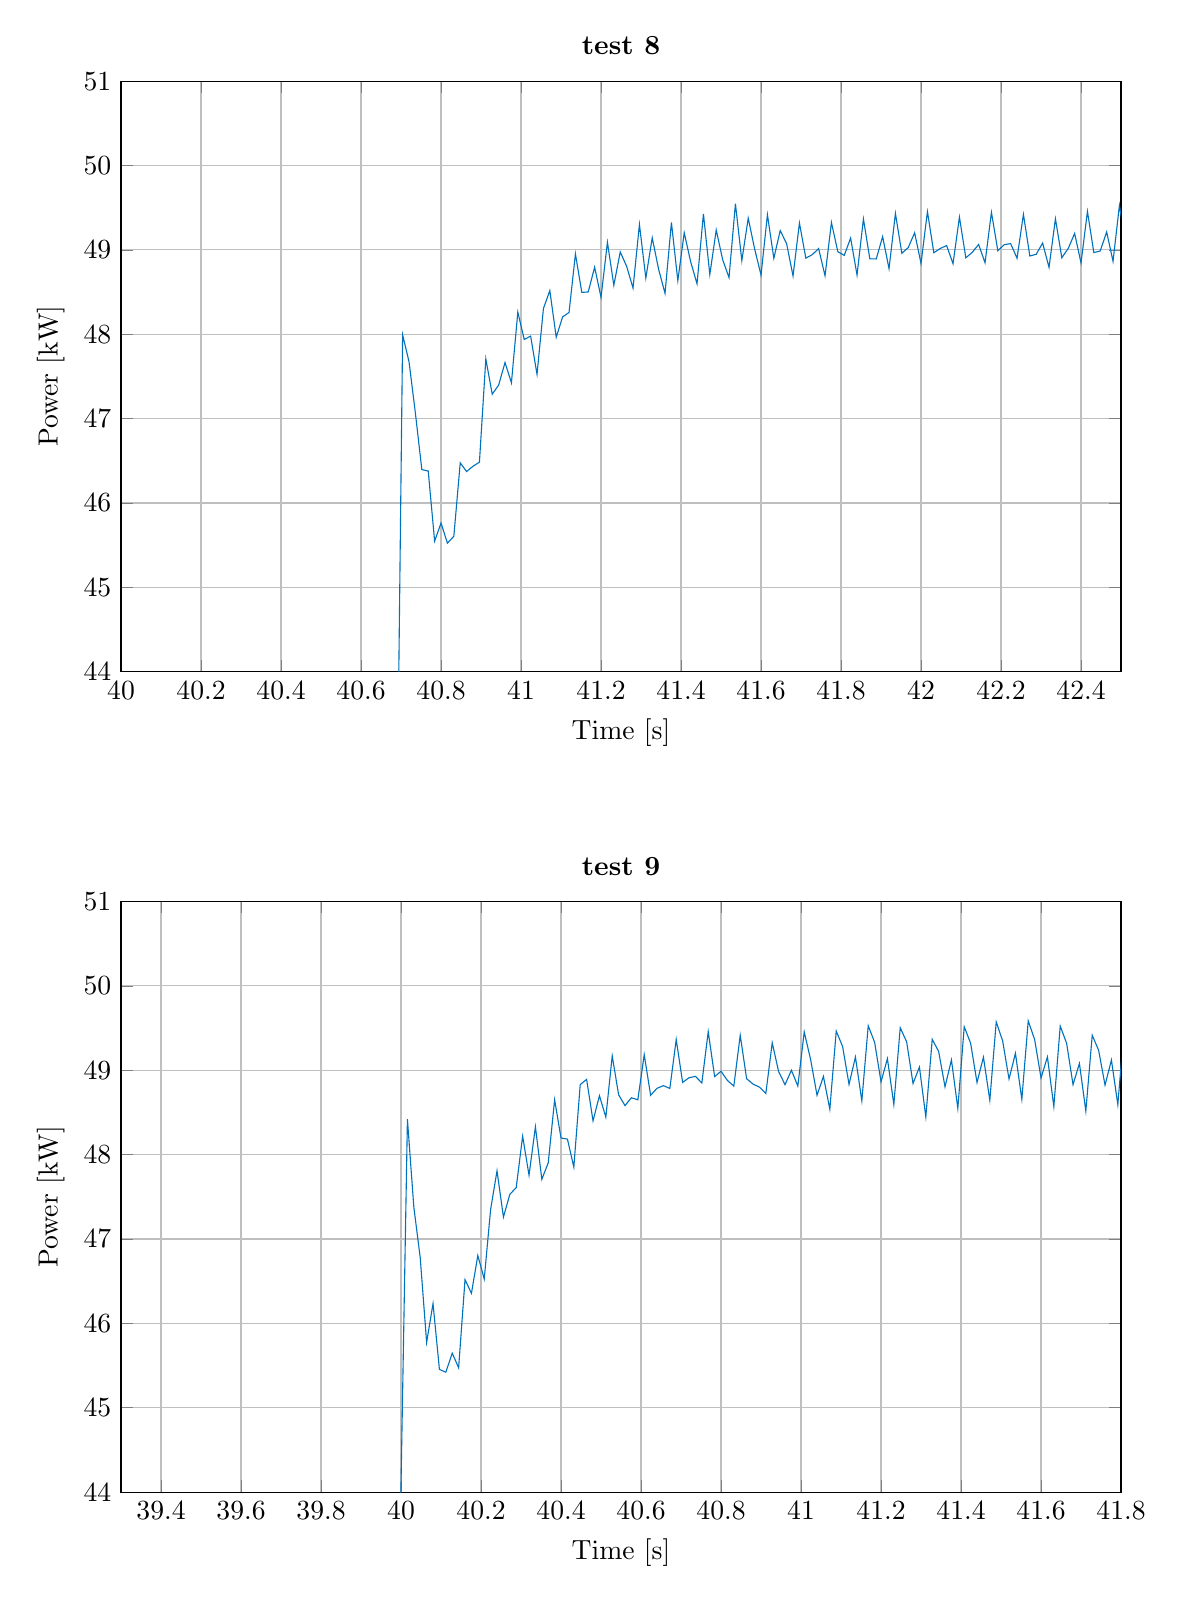
\begin{tikzpicture}

\begin{axis}[%
width=5in,
height=2.953in,
at={(1.142in,5.054in)},
scale only axis,
xmin=40,
xmax=42.5,
xlabel={Time [s]},
xmajorgrids,
ymin=44,
ymax=51,
ylabel={Power [kW]},
ymajorgrids,
axis background/.style={fill=white},
title style={font=\bfseries},
title={test 8}
]
\addplot [color=mycolor1,solid,forget plot]
  table[row sep=crcr]{%
40.6927847910867	43.3\\
40.704	47.9929472503775\\
40.72	47.6738190307726\\
40.736	47.0609812801745\\
40.752	46.3960385668663\\
40.768	46.3785059021049\\
40.784	45.5473457934362\\
40.8	45.7616622620457\\
40.816	45.524103848115\\
40.832	45.6043828950495\\
40.848	46.4752717165229\\
40.864	46.3727056625158\\
40.88	46.4351531348534\\
40.896	46.4833091303381\\
40.912	47.707803556809\\
40.928	47.2892914203898\\
40.944	47.3965683469461\\
40.96	47.6644408705848\\
40.976	47.4248403393385\\
40.992	48.2626615742331\\
41.008	47.9381213411157\\
41.024	47.9773642333031\\
41.04	47.5250460334631\\
41.056	48.3043751683031\\
41.072	48.5169171470674\\
41.088	47.9644956611792\\
41.104	48.2058850913389\\
41.12	48.2568569325432\\
41.136	48.9515813156737\\
41.152	48.4957478598312\\
41.168	48.5010681616608\\
41.184	48.7944320936071\\
41.2	48.4369596524744\\
41.216	49.0897459747431\\
41.232	48.5799543863284\\
41.248	48.9750088588145\\
41.264	48.8055582248958\\
41.28	48.5464193115349\\
41.296	49.300922156118\\
41.312	48.6653817723916\\
41.328	49.1425370225463\\
41.344	48.7687722188269\\
41.36	48.4844641444414\\
41.376	49.324152358638\\
41.392	48.6350214550147\\
41.408	49.202593085456\\
41.424	48.8602784587096\\
41.44	48.5974682496596\\
41.456	49.4266062432109\\
41.472	48.707695097148\\
41.488	49.2356620121912\\
41.504	48.884755453913\\
41.52	48.6716472869057\\
41.536	49.5464026288743\\
41.552	48.8721617063946\\
41.568	49.3753181461739\\
41.584	49.0115874283828\\
41.6	48.7008941079675\\
41.616	49.4165211524875\\
41.632	48.8999179760452\\
41.648	49.2287738383106\\
41.664	49.0724608635199\\
41.68	48.6899391939282\\
41.696	49.3179885203791\\
41.712	48.9017468328818\\
41.728	48.9424984434456\\
41.744	49.0152460500126\\
41.76	48.692849215118\\
41.776	49.3241100201983\\
41.792	48.9783964447865\\
41.808	48.9344032297057\\
41.824	49.1401915033668\\
41.84	48.7018401623785\\
41.856	49.3662489101383\\
41.872	48.893595896562\\
41.888	48.8921315167007\\
41.904	49.1568101048654\\
41.92	48.776492688748\\
41.936	49.4314043659678\\
41.952	48.9596894408704\\
41.968	49.0265059654831\\
41.984	49.2020639084303\\
42	48.8390631088736\\
42.016	49.4536651493048\\
42.032	48.9660751009307\\
42.048	49.0163533980249\\
42.064	49.0505184612856\\
42.08	48.835930340501\\
42.096	49.3888023417642\\
42.112	48.9054676056902\\
42.128	48.9698557859391\\
42.144	49.0640991102677\\
42.16	48.8468138204933\\
42.176	49.4436263989268\\
42.192	48.9890835971507\\
42.208	49.0609949458161\\
42.224	49.0743663181223\\
42.24	48.8998156700772\\
42.256	49.42053106804\\
42.272	48.9270616416261\\
42.288	48.9477390516098\\
42.304	49.080480075535\\
42.32	48.7924157602473\\
42.336	49.3687076167259\\
42.352	48.9066994504617\\
42.368	49.0163498284249\\
42.384	49.1951441980053\\
42.4	48.8439541869268\\
42.416	49.4566588768984\\
42.432	48.9676669766432\\
42.448	48.9856884969546\\
42.464	49.2131667673939\\
42.48	48.8642407773787\\
42.496	49.5269718940021\\
42.512	49.0641461334\\
};
\end{axis}

\begin{axis}[%
width=5in,
height=2.953in,
at={(1.142in,0.952in)},
scale only axis,
xmin=39.3,
xmax=41.8,
xlabel={Time [s]},
xmajorgrids,
ymin=44,
ymax=51,
ylabel={Power [kW]},
ymajorgrids,
axis background/.style={fill=white},
title style={font=\bfseries},
title={test 9}
]
\addplot [color=mycolor1,solid,forget plot]
  table[row sep=crcr]{%
39.9975826382822	43.3\\
40	44.099738983591\\
40.016	48.4189906383941\\
40.032	47.3788802327897\\
40.048	46.778172676322\\
40.064	45.7739421337619\\
40.08	46.2342768138171\\
40.096	45.4541102927374\\
40.112	45.4209302998728\\
40.128	45.6466222218855\\
40.144	45.4740092366158\\
40.16	46.5184317816815\\
40.176	46.3561600892903\\
40.192	46.8045467123484\\
40.208	46.5258542843183\\
40.224	47.3509366276498\\
40.24	47.807042091978\\
40.256	47.2600401687991\\
40.272	47.5283706884958\\
40.288	47.6098754997116\\
40.304	48.2180528763904\\
40.32	47.755729667244\\
40.336	48.3299976408664\\
40.352	47.7071923496876\\
40.368	47.9020780171937\\
40.384	48.6497044170826\\
40.4	48.1967003003206\\
40.416	48.1839681657318\\
40.432	47.8519738727675\\
40.448	48.8298141237524\\
40.464	48.8916443425237\\
40.48	48.4000980004466\\
40.496	48.6986064598599\\
40.512	48.4446924875794\\
40.528	49.1696940979228\\
40.544	48.7084808624788\\
40.56	48.5809943937504\\
40.576	48.6739685301351\\
40.592	48.649544695461\\
40.608	49.1845124285581\\
40.624	48.7029477094668\\
40.64	48.7859862161165\\
40.656	48.817397461607\\
40.672	48.7841813994213\\
40.688	49.3641507559289\\
40.704	48.8555954121368\\
40.72	48.9111086181275\\
40.736	48.9277054582452\\
40.752	48.8494966143881\\
40.768	49.4566493766976\\
40.784	48.925121243645\\
40.8	48.9878939942235\\
40.816	48.878992018107\\
40.832	48.8121870817406\\
40.848	49.4145901599559\\
40.864	48.899437284972\\
40.88	48.8361213770869\\
40.896	48.8000331537413\\
40.912	48.7240753474837\\
40.928	49.3256012848323\\
40.944	48.9842985113072\\
40.96	48.8293832618908\\
40.976	49.0000661019471\\
40.992	48.8128347786239\\
41.008	49.4544596665934\\
41.024	49.1255896451435\\
41.04	48.7039145738355\\
41.056	48.9270056980748\\
41.072	48.5380310857453\\
41.088	49.4639487637534\\
41.104	49.281084084961\\
41.12	48.8323763628567\\
41.136	49.1569839837637\\
41.152	48.6373160420227\\
41.168	49.5268655808502\\
41.184	49.3316441337109\\
41.2	48.8627289117392\\
41.216	49.1377584105911\\
41.232	48.5943231077482\\
41.248	49.5037292417081\\
41.264	49.3373170392993\\
41.28	48.8435191817643\\
41.296	49.0375813671902\\
41.312	48.4468306961557\\
41.328	49.366998570664\\
41.344	49.2236695864775\\
41.36	48.8035124873272\\
41.376	49.1227252661862\\
41.392	48.5477694051544\\
41.408	49.5153134161183\\
41.424	49.3202913789668\\
41.44	48.8543583754286\\
41.456	49.1555857981871\\
41.472	48.6448789132256\\
41.488	49.5724476463382\\
41.504	49.3486620208636\\
41.52	48.8960338986448\\
41.536	49.2012602067504\\
41.552	48.6552406810012\\
41.568	49.5846743211034\\
41.584	49.3636555167402\\
41.6	48.9084884851888\\
41.616	49.1573816257077\\
41.632	48.5703606374812\\
41.648	49.5239056334283\\
41.664	49.3189221916061\\
41.68	48.8300805293604\\
41.696	49.0804774933847\\
41.712	48.5163421966984\\
41.728	49.4141932650679\\
41.744	49.2373594417614\\
41.76	48.8238670713629\\
41.776	49.1220139469627\\
41.792	48.592514438109\\
41.808	49.5048782138206\\
};
\end{axis}
\end{tikzpicture}%
% \caption{Power disturbance on the output of the genset occuring from step of 40 to 50 kW load.}
% \label{fig:test8-9-40to50kwsteppower}
% \end{figure}

% \begin{figure}[H]
% \centering
% % This file was created by matlab2tikz.
%
%The latest updates can be retrieved from
%  http://www.mathworks.com/matlabcentral/fileexchange/22022-matlab2tikz-matlab2tikz
%where you can also make suggestions and rate matlab2tikz.
%
\definecolor{mycolor1}{rgb}{0.00000,0.44700,0.74100}%
%
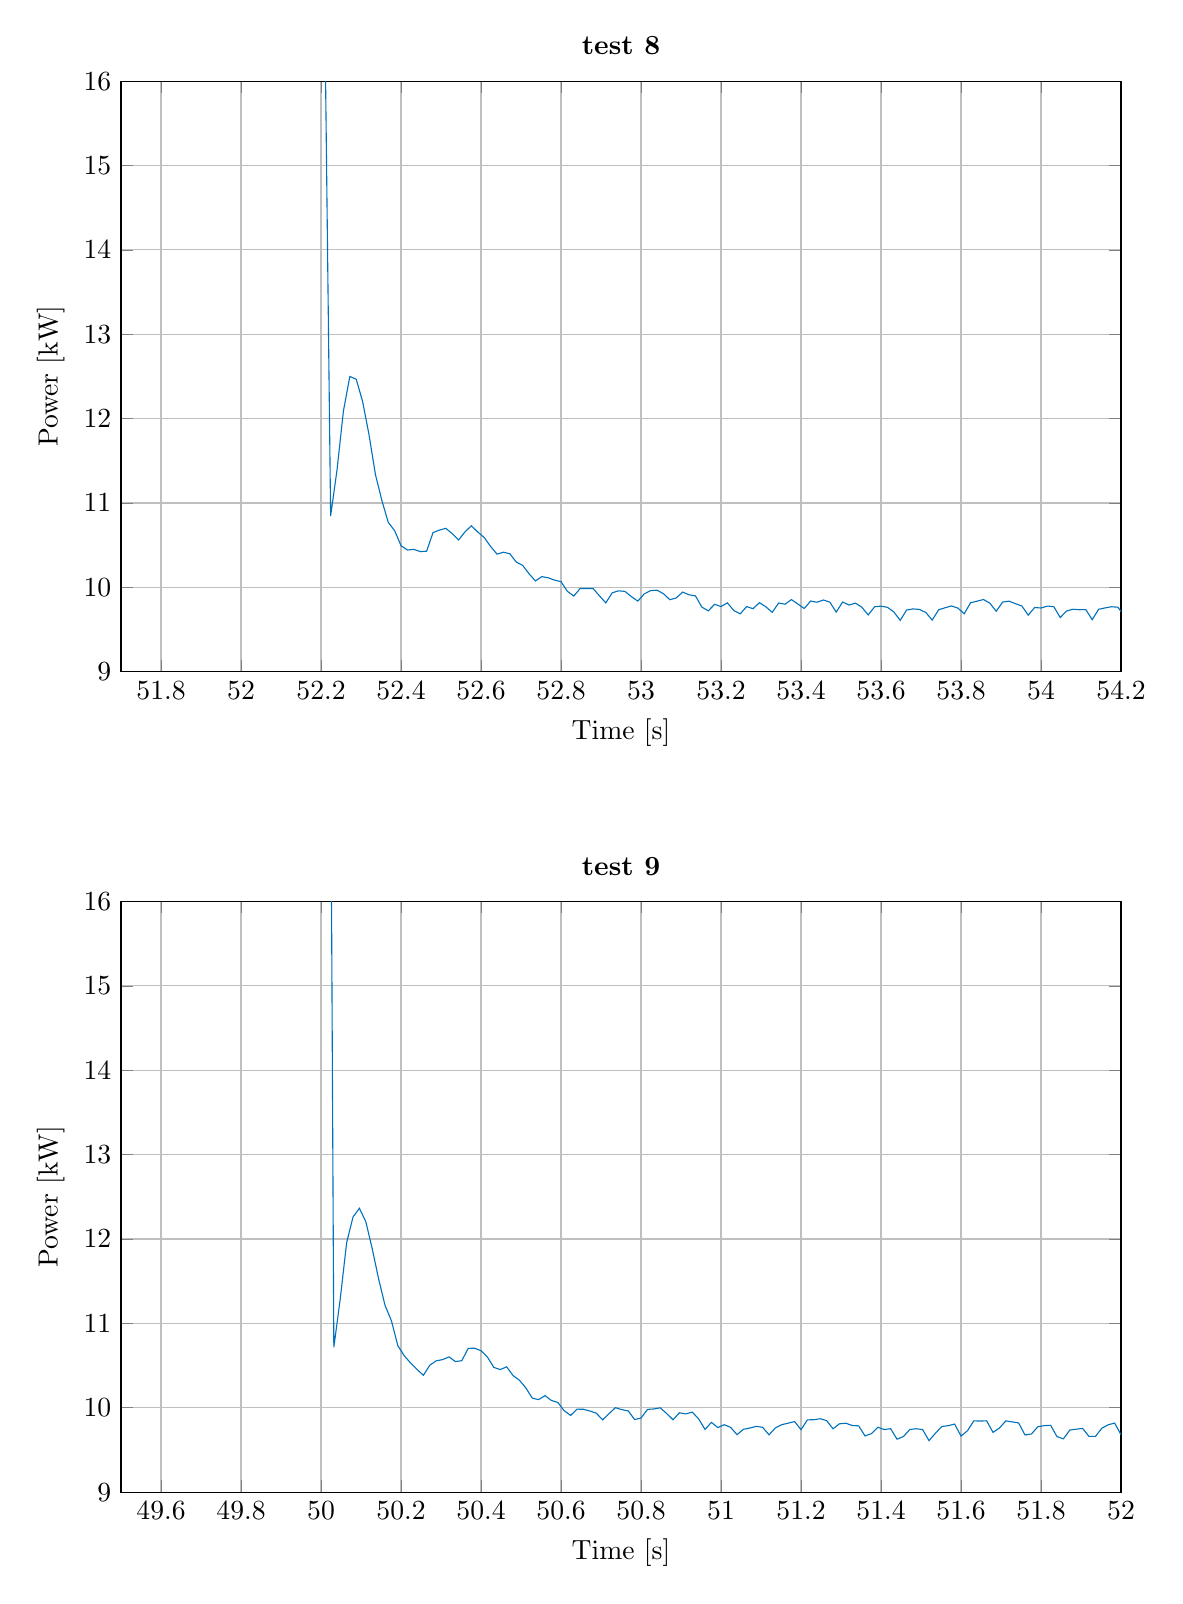
\begin{tikzpicture}

\begin{axis}[%
width=5in,
height=2.953in,
at={(1.142in,5.054in)},
scale only axis,
xmin=51.7,
xmax=54.2,
xlabel={Time [s]},
xmajorgrids,
ymin=9,
ymax=16,
ylabel={Power [kW]},
ymajorgrids,
axis background/.style={fill=white},
title style={font=\bfseries},
title={test 8}
]
\addplot [color=mycolor1,solid,forget plot]
  table[row sep=crcr]{%
52.209722075348	16.7\\
52.224	10.8454277316002\\
52.24	11.3917822783096\\
52.256	12.0902655967483\\
52.272	12.4988837780916\\
52.288	12.4668012010825\\
52.304	12.2019261784565\\
52.32	11.8080260166184\\
52.336	11.3377018613142\\
52.352	11.0314266727299\\
52.368	10.770957547222\\
52.384	10.6720791863803\\
52.4	10.4936585004037\\
52.416	10.4423063620685\\
52.432	10.4501306899826\\
52.448	10.4235828117714\\
52.464	10.428135775883\\
52.48	10.6486133567073\\
52.496	10.6786615303812\\
52.512	10.6992155711045\\
52.528	10.6365360949875\\
52.544	10.5616320747563\\
52.56	10.658093368739\\
52.576	10.7299661269566\\
52.592	10.6548723186293\\
52.608	10.5904827473734\\
52.624	10.4839557280502\\
52.64	10.3931392345789\\
52.656	10.4159468112669\\
52.672	10.3978715457745\\
52.688	10.3001128335324\\
52.704	10.2606398698784\\
52.72	10.1612217010941\\
52.736	10.0758845284196\\
52.752	10.127014181502\\
52.768	10.1129165829184\\
52.784	10.0850804823855\\
52.8	10.0673538853798\\
52.816	9.95180196892617\\
52.832	9.8967414280182\\
52.848	9.98704746925522\\
52.864	9.985360598062\\
52.88	9.98685304076431\\
52.896	9.89926944148228\\
52.912	9.81572702355126\\
52.928	9.934842790373\\
52.944	9.95867272960641\\
52.96	9.95146601060655\\
52.976	9.88952530427732\\
52.992	9.83676780314892\\
53.008	9.92224321507843\\
53.024	9.96068945932651\\
53.04	9.96612280716447\\
53.056	9.92492708030495\\
53.072	9.85328891321493\\
53.088	9.87457706938206\\
53.104	9.94318460647274\\
53.12	9.91134596999997\\
53.136	9.89905684719209\\
53.152	9.76627902896019\\
53.168	9.72107859888972\\
53.184	9.79893572180445\\
53.2	9.77216922590819\\
53.216	9.8156311313186\\
53.232	9.72475101140077\\
53.248	9.68560882675938\\
53.264	9.77215527611179\\
53.28	9.74674320604248\\
53.296	9.81814354160649\\
53.312	9.76981720425158\\
53.328	9.70333028815132\\
53.344	9.81406284383742\\
53.36	9.80008227434268\\
53.376	9.85459968113531\\
53.392	9.80245359372258\\
53.408	9.74901663867218\\
53.424	9.8374235770084\\
53.44	9.82340576878566\\
53.456	9.85010142948912\\
53.472	9.82444495429531\\
53.488	9.70655866326442\\
53.504	9.82615201138492\\
53.52	9.7898376916258\\
53.536	9.81241843058366\\
53.552	9.76445539729912\\
53.568	9.67283436340877\\
53.584	9.76983663360582\\
53.6	9.77714612465992\\
53.616	9.76298997616599\\
53.632	9.70858565513602\\
53.648	9.60909106937996\\
53.664	9.73094693559097\\
53.68	9.74410808931599\\
53.696	9.73809473233844\\
53.712	9.70168140318441\\
53.728	9.61210492460277\\
53.744	9.7335938955521\\
53.76	9.75740069780171\\
53.776	9.77967845625081\\
53.792	9.75382081030809\\
53.808	9.6873492668739\\
53.824	9.81760952410011\\
53.84	9.83593027484933\\
53.856	9.8555453227451\\
53.872	9.81213896548404\\
53.888	9.71635945569496\\
53.904	9.82507610506005\\
53.92	9.83632509926968\\
53.936	9.80641234235284\\
53.952	9.77899142550802\\
53.968	9.6699752250687\\
53.984	9.76062780826478\\
54	9.75516616360608\\
54.016	9.77772790855606\\
54.032	9.77026163781028\\
54.048	9.64213786580116\\
54.064	9.7193349287812\\
54.08	9.74007182307863\\
54.096	9.73467117498306\\
54.112	9.73592352206309\\
54.128	9.61669511542732\\
54.144	9.73996269287082\\
54.16	9.75572256290835\\
54.176	9.76994111386167\\
54.192	9.76438635513565\\
54.208	9.66592701693149\\
};
\end{axis}

\begin{axis}[%
width=5in,
height=2.953in,
at={(1.142in,0.952in)},
scale only axis,
xmin=49.5,
xmax=52,
xlabel={Time [s]},
xmajorgrids,
ymin=9,
ymax=16,
ylabel={Power [kW]},
ymajorgrids,
axis background/.style={fill=white},
title style={font=\bfseries},
title={test 9}
]
\addplot [color=mycolor1,solid,forget plot]
  table[row sep=crcr]{%
50.0255030493245	16.7\\
50.032	10.7160992188925\\
50.048	11.2876422038713\\
50.064	11.9550392250216\\
50.08	12.261265973303\\
50.096	12.3638442250084\\
50.112	12.2050076987081\\
50.128	11.8851141257187\\
50.144	11.5259541700897\\
50.16	11.2139828900154\\
50.176	11.0306908804755\\
50.192	10.7355730739739\\
50.208	10.6163524685762\\
50.224	10.5301060777113\\
50.24	10.4534496741731\\
50.256	10.3848212005821\\
50.272	10.5043804613222\\
50.288	10.5560723448987\\
50.304	10.5704504892233\\
50.32	10.6024226771619\\
50.336	10.5468213095297\\
50.352	10.5580483927568\\
50.368	10.703795484899\\
50.384	10.7054280510947\\
50.4	10.6756858278884\\
50.416	10.6003922561425\\
50.432	10.4782981161471\\
50.448	10.4522513708122\\
50.464	10.4845479438016\\
50.48	10.3819659694568\\
50.496	10.3261575967686\\
50.512	10.2359434149587\\
50.528	10.1140032579348\\
50.544	10.0960207421461\\
50.56	10.1435565985375\\
50.576	10.0859694698402\\
50.592	10.0626617961426\\
50.608	9.96408085635851\\
50.624	9.90977195257771\\
50.64	9.9828165846281\\
50.656	9.98230235271927\\
50.672	9.96149465403765\\
50.688	9.93626376016517\\
50.704	9.8563388324237\\
50.72	9.92989175895325\\
50.736	10.0008553050698\\
50.752	9.97708819920659\\
50.768	9.96188206476859\\
50.784	9.86040605018689\\
50.8	9.87733521436597\\
50.816	9.97976481027674\\
50.832	9.98560222185481\\
50.848	9.99923864294004\\
50.864	9.93195734450165\\
50.88	9.85761360581789\\
50.896	9.94013113810276\\
50.912	9.92666255535793\\
50.928	9.94836280534677\\
50.944	9.86825143290018\\
50.96	9.74294268743944\\
50.976	9.82690888118142\\
50.992	9.76452101795562\\
51.008	9.79888730878937\\
51.024	9.76763526422081\\
51.04	9.68068646906558\\
51.056	9.74464252437281\\
51.072	9.75926475073558\\
51.088	9.7792550167707\\
51.104	9.76790397965947\\
51.12	9.67863969622579\\
51.136	9.76077477379423\\
51.152	9.79952222363202\\
51.168	9.81726004682256\\
51.184	9.83631146094162\\
51.2	9.73978712869128\\
51.216	9.85634269027488\\
51.232	9.85819373398665\\
51.248	9.86958258105178\\
51.264	9.84738084913902\\
51.28	9.75033209987679\\
51.296	9.80948241466555\\
51.312	9.81638271878305\\
51.328	9.78953228106112\\
51.344	9.78511144826493\\
51.36	9.66581270476419\\
51.376	9.69312246909939\\
51.392	9.76871412950726\\
51.408	9.74130035341403\\
51.424	9.75190158776002\\
51.44	9.62747383643393\\
51.456	9.65823264863109\\
51.472	9.74182902025638\\
51.488	9.75124056221884\\
51.504	9.74039438385295\\
51.52	9.60999833245861\\
51.536	9.69759132414116\\
51.552	9.77805655306529\\
51.568	9.7874042728983\\
51.584	9.80630777738985\\
51.6	9.66390550961506\\
51.616	9.7266750625251\\
51.632	9.84469714568904\\
51.648	9.84200573010952\\
51.664	9.84505030994884\\
51.68	9.70796988872221\\
51.696	9.75917266757954\\
51.712	9.84422061593478\\
51.728	9.83171480082745\\
51.744	9.81999054982033\\
51.76	9.67684754168791\\
51.776	9.68873917689973\\
51.792	9.77448056749409\\
51.808	9.78821322551062\\
51.824	9.79175841021768\\
51.84	9.65717928456695\\
51.856	9.63137677319806\\
51.872	9.73561760014464\\
51.888	9.74577020533451\\
51.904	9.75493411874404\\
51.92	9.65987748562842\\
51.936	9.65994505759101\\
51.952	9.75659627828239\\
51.968	9.797781652192\\
51.984	9.81822207998591\\
52	9.68014736933464\\
52.016	9.70444045767485\\
};
\end{axis}
\end{tikzpicture}%
% \caption{Power disturbance on the output of the genset occuring from step of 50 to 10 kW load.}
% \label{fig:test8-9-50to10kwsteppower}
% \end{figure}

%---------------------------------------------------
\subsubsection*{Volt}
\begin{figure}[H]
\centering
% This file was created by matlab2tikz.
%
%The latest updates can be retrieved from
%  http://www.mathworks.com/matlabcentral/fileexchange/22022-matlab2tikz-matlab2tikz
%where you can also make suggestions and rate matlab2tikz.
%
\definecolor{mycolor1}{rgb}{0.00000,0.44700,0.74100}%
%
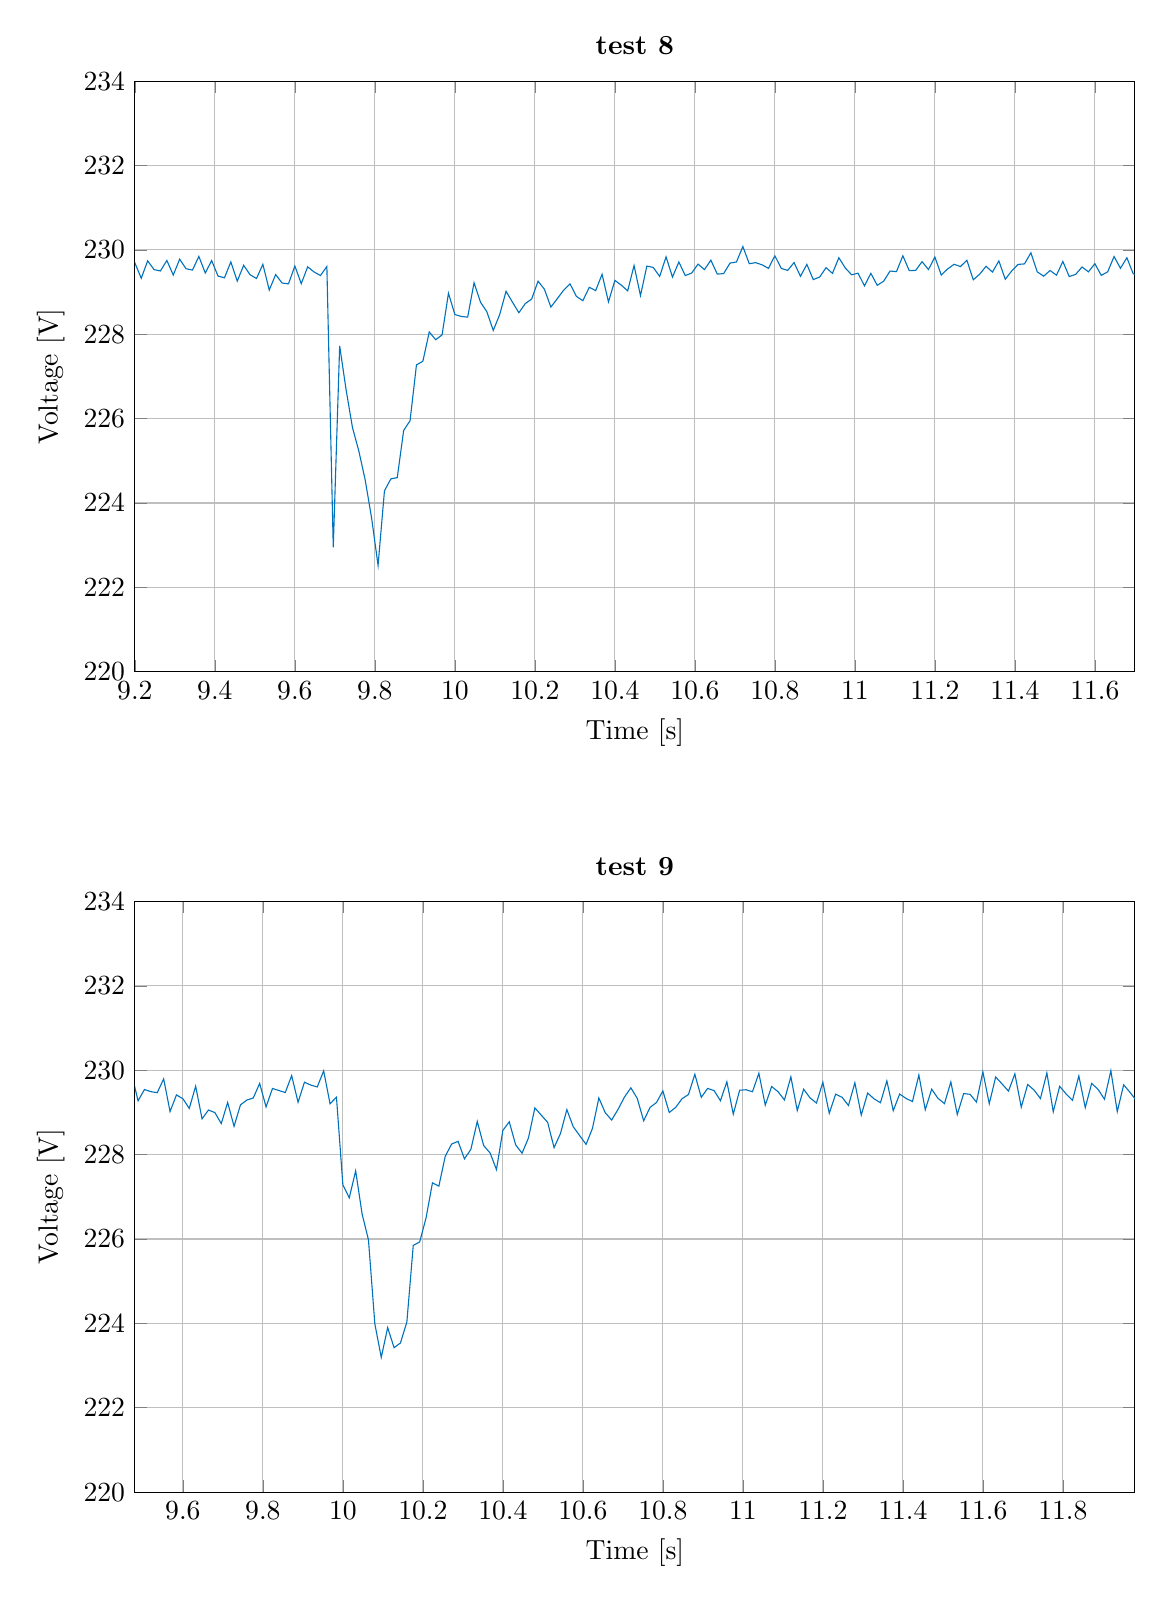
\begin{tikzpicture}

\begin{axis}[%
width=5in,
height=2.953in,
at={(1.142in,5.054in)},
scale only axis,
xmin=9.2,
xmax=11.7,
xlabel={Time [s]},
xmajorgrids,
ymin=220,
ymax=234,
ylabel={Voltage [V]},
ymajorgrids,
axis background/.style={fill=white},
title style={font=\bfseries},
title={test 8}
]
\addplot [color=mycolor1,solid,forget plot]
  table[row sep=crcr]{%
9.184	229.410630632502\\
9.2	229.690715335454\\
9.216	229.32701959224\\
9.232	229.738831127096\\
9.248	229.531921207839\\
9.264	229.499778977419\\
9.28	229.748666228288\\
9.296	229.402335901126\\
9.312	229.778648637495\\
9.328	229.552587262574\\
9.344	229.520188995313\\
9.36	229.844554733724\\
9.376	229.451218952181\\
9.392	229.745264506417\\
9.408	229.376655402668\\
9.424	229.338926191208\\
9.44	229.714703147942\\
9.456	229.259034065655\\
9.472	229.633664557694\\
9.488	229.410466278477\\
9.504	229.320376277629\\
9.52	229.656627794122\\
9.536	229.047379988031\\
9.552	229.413341060431\\
9.568	229.215095147076\\
9.584	229.193362053371\\
9.6	229.617002774202\\
9.616	229.197764611183\\
9.632	229.596344664625\\
9.648	229.475804245851\\
9.664	229.391211353035\\
9.68	229.605324675344\\
9.696	222.947772817164\\
9.712	227.724009479168\\
9.728	226.688114047742\\
9.744	225.788274293474\\
9.76	225.22795799241\\
9.776	224.538086593297\\
9.792	223.631745354665\\
9.808	222.519419171351\\
9.824	224.288439164994\\
9.84	224.570635868611\\
9.856	224.601547790095\\
9.872	225.719076936514\\
9.888	225.950982357793\\
9.904	227.273086249086\\
9.92	227.358468008874\\
9.936	228.05377214986\\
9.952	227.869386718192\\
9.968	227.983388011283\\
9.984	228.971409444748\\
10	228.466537252619\\
10.016	228.421633478975\\
10.032	228.405105547057\\
10.048	229.221100314441\\
10.064	228.760825869602\\
10.08	228.532696847045\\
10.096	228.090022424992\\
10.112	228.463376899668\\
10.128	229.018342404364\\
10.144	228.759899013698\\
10.16	228.509443801909\\
10.176	228.725843657976\\
10.192	228.834304108031\\
10.208	229.257753846356\\
10.224	229.063706554168\\
10.24	228.643485490637\\
10.256	228.841323528064\\
10.272	229.04374567414\\
10.288	229.192320686901\\
10.304	228.895262954532\\
10.32	228.794609741371\\
10.336	229.111513022069\\
10.352	229.034101520775\\
10.368	229.420721670777\\
10.384	228.766136598018\\
10.4	229.275727071853\\
10.416	229.164062383815\\
10.432	229.028226167243\\
10.448	229.628097612003\\
10.464	228.915640051849\\
10.48	229.614763071499\\
10.496	229.582950272004\\
10.512	229.370278682605\\
10.528	229.834532589427\\
10.544	229.354844610515\\
10.56	229.711731772298\\
10.576	229.39070999571\\
10.592	229.449556565817\\
10.608	229.662014487451\\
10.624	229.530935945904\\
10.64	229.755691703703\\
10.656	229.424708576421\\
10.672	229.437684006142\\
10.688	229.686379524498\\
10.704	229.712631146526\\
10.72	230.079258905402\\
10.736	229.672015641485\\
10.752	229.696901553342\\
10.768	229.645777435992\\
10.784	229.560341540848\\
10.8	229.859435328326\\
10.816	229.55989778995\\
10.832	229.512689965262\\
10.848	229.698840715079\\
10.864	229.371954240125\\
10.88	229.654924984385\\
10.896	229.2947825531\\
10.912	229.356347948928\\
10.928	229.577444423169\\
10.944	229.442725901894\\
10.96	229.813756351569\\
10.976	229.569979919468\\
10.992	229.408801163032\\
11.008	229.447101175542\\
11.024	229.145527089646\\
11.04	229.443546184263\\
11.056	229.1574752057\\
11.072	229.258036890033\\
11.088	229.497220705871\\
11.104	229.483568806696\\
11.12	229.859586306746\\
11.136	229.506542493657\\
11.152	229.513041286626\\
11.168	229.720058906553\\
11.184	229.533129909852\\
11.2	229.829820100242\\
11.216	229.403163795558\\
11.232	229.548606841975\\
11.248	229.65709065265\\
11.264	229.604812583615\\
11.28	229.753778675755\\
11.296	229.291097744418\\
11.312	229.422488199705\\
11.328	229.610765164278\\
11.344	229.472493171246\\
11.36	229.737158830792\\
11.376	229.303233686802\\
11.392	229.498380954304\\
11.408	229.655063746236\\
11.424	229.66626063156\\
11.44	229.929589063192\\
11.456	229.477204685177\\
11.472	229.375856823907\\
11.488	229.510764814287\\
11.504	229.399636110155\\
11.52	229.724659854149\\
11.536	229.36654440335\\
11.552	229.418751891406\\
11.568	229.593564382283\\
11.584	229.479247883539\\
11.6	229.672368530792\\
11.616	229.394789176272\\
11.632	229.479205056294\\
11.648	229.840953335016\\
11.664	229.563198514071\\
11.68	229.812745090211\\
11.696	229.430460460626\\
11.712	229.396725970643\\
};
\end{axis}

\begin{axis}[%
width=5in,
height=2.953in,
at={(1.142in,0.952in)},
scale only axis,
xmin=9.48,
xmax=11.98,
xlabel={Time [s]},
xmajorgrids,
ymin=220,
ymax=234,
ylabel={Voltage [V]},
ymajorgrids,
axis background/.style={fill=white},
title style={font=\bfseries},
title={test 9}
]
\addplot [color=mycolor1,solid,forget plot]
  table[row sep=crcr]{%
9.472	229.911006170757\\
9.488	229.274375507886\\
9.504	229.543776718558\\
9.52	229.492890816935\\
9.536	229.467821581187\\
9.552	229.795446772667\\
9.568	229.021635849397\\
9.584	229.415140784778\\
9.6	229.325503078225\\
9.616	229.09496167773\\
9.632	229.623068988749\\
9.648	228.847362680231\\
9.664	229.056163931565\\
9.68	228.997412815041\\
9.696	228.736033840157\\
9.712	229.236596572513\\
9.728	228.670522243599\\
9.744	229.178631310203\\
9.76	229.29410461216\\
9.776	229.342477882471\\
9.792	229.687545814813\\
9.808	229.1316737941\\
9.824	229.568096704931\\
9.84	229.520010644539\\
9.856	229.471511209308\\
9.872	229.873145709938\\
9.888	229.241578887697\\
9.904	229.716324118121\\
9.92	229.647679234758\\
9.936	229.603880082647\\
9.952	229.985041579959\\
9.968	229.204423335532\\
9.984	229.362049787947\\
10	227.286051449423\\
10.016	226.975659899619\\
10.032	227.615390877728\\
10.048	226.598594656399\\
10.064	225.978803325171\\
10.08	223.985557339732\\
10.096	223.193901119016\\
10.112	223.899513770813\\
10.128	223.423981032391\\
10.144	223.536199188498\\
10.16	224.031957612913\\
10.176	225.848883640993\\
10.192	225.929390347255\\
10.208	226.500713732105\\
10.224	227.330977552075\\
10.24	227.253975733515\\
10.256	227.962367955831\\
10.272	228.25153001775\\
10.288	228.315074626648\\
10.304	227.899917943474\\
10.32	228.123054967152\\
10.336	228.78552944497\\
10.352	228.215389929944\\
10.368	228.040164102252\\
10.384	227.645408756927\\
10.4	228.574047639057\\
10.416	228.77866200403\\
10.432	228.231301600194\\
10.448	228.033281980103\\
10.464	228.395149005253\\
10.48	229.107534093284\\
10.496	228.935538251964\\
10.512	228.765034175317\\
10.528	228.165476022307\\
10.544	228.499995651701\\
10.56	229.066956748066\\
10.576	228.659940243084\\
10.592	228.450590006882\\
10.608	228.243390192446\\
10.624	228.622631189628\\
10.64	229.342090047596\\
10.656	228.993840036505\\
10.672	228.819657655979\\
10.688	229.073541845342\\
10.704	229.364208086494\\
10.72	229.584240951846\\
10.736	229.3318348226\\
10.752	228.801969402338\\
10.768	229.12034546599\\
10.784	229.234219447126\\
10.8	229.510084246484\\
10.816	228.998536385059\\
10.832	229.119705311668\\
10.848	229.325682004143\\
10.864	229.424496152537\\
10.88	229.903735966784\\
10.896	229.358286582565\\
10.912	229.569909454448\\
10.928	229.519147357713\\
10.944	229.277118954856\\
10.96	229.728282250787\\
10.976	228.958218467177\\
10.992	229.52636020796\\
11.008	229.538062908048\\
11.024	229.489856320472\\
11.04	229.928292960095\\
11.056	229.173434952205\\
11.072	229.614378943307\\
11.088	229.491163320831\\
11.104	229.295902742487\\
11.12	229.845670808963\\
11.136	229.045211008723\\
11.152	229.549330198194\\
11.168	229.344519820614\\
11.184	229.223992758699\\
11.2	229.715478848324\\
11.216	228.979837377926\\
11.232	229.432463959089\\
11.248	229.359650570164\\
11.264	229.164460606275\\
11.28	229.702092497972\\
11.296	228.937468988611\\
11.312	229.458129451825\\
11.328	229.322490464546\\
11.344	229.231028265807\\
11.36	229.748471731126\\
11.376	229.041572397287\\
11.392	229.436737573572\\
11.408	229.33125647174\\
11.424	229.258494409694\\
11.44	229.886807297472\\
11.456	229.062795615996\\
11.472	229.550392193772\\
11.488	229.332161481399\\
11.504	229.210058038512\\
11.52	229.723383822923\\
11.536	228.950694195735\\
11.552	229.447197286568\\
11.568	229.429814296043\\
11.584	229.244899938999\\
11.6	229.964165476905\\
11.616	229.206629628638\\
11.632	229.839222876742\\
11.648	229.675978464941\\
11.664	229.504948230286\\
11.68	229.914760330419\\
11.696	229.124256038509\\
11.712	229.662291339363\\
11.728	229.530443112568\\
11.744	229.328763582754\\
11.76	229.937960950325\\
11.776	229.015648905361\\
11.792	229.61849980074\\
11.808	229.440217595696\\
11.824	229.286187447475\\
11.84	229.8654021203\\
11.856	229.113833488598\\
11.872	229.688098551014\\
11.888	229.54723208775\\
11.904	229.313647967539\\
11.92	229.988723508108\\
11.936	229.019548020191\\
11.952	229.653922630344\\
11.968	229.47524001792\\
11.984	229.276732535723\\
};
\end{axis}
\end{tikzpicture}%
\caption{Voltage disturbance on the output of the genset occuring from step of 10 to 20 kW load.}
\label{fig:test8-9-10to20kwstepvolt}
\end{figure}

\begin{figure}[H]
\centering
% This file was created by matlab2tikz.
%
%The latest updates can be retrieved from
%  http://www.mathworks.com/matlabcentral/fileexchange/22022-matlab2tikz-matlab2tikz
%where you can also make suggestions and rate matlab2tikz.
%
\definecolor{mycolor1}{rgb}{0.00000,0.44700,0.74100}%
%
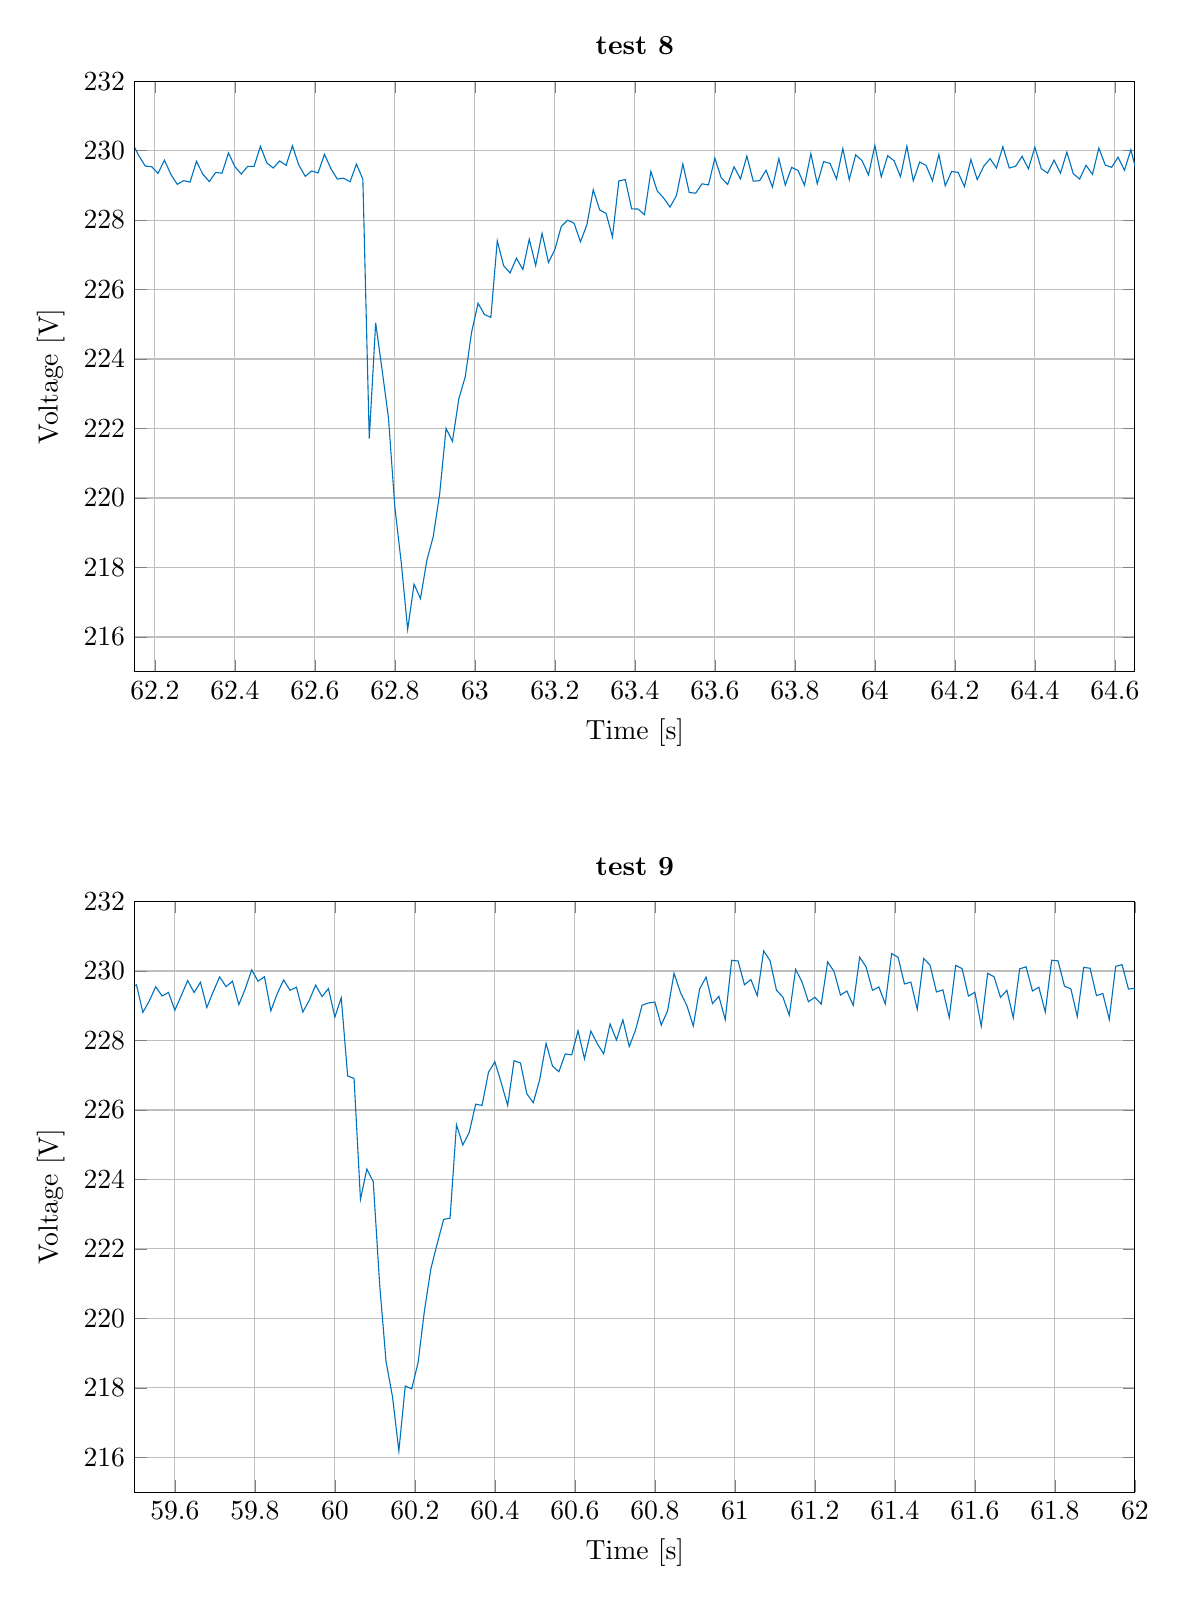
\begin{tikzpicture}

\begin{axis}[%
width=5in,
height=2.953in,
at={(1.142in,5.054in)},
scale only axis,
xmin=62.15,
xmax=64.65,
xlabel={Time [s]},
xmajorgrids,
ymin=215,
ymax=232,
ylabel={Voltage [V]},
ymajorgrids,
axis background/.style={fill=white},
title style={font=\bfseries},
title={test 8}
]
\addplot [color=mycolor1,solid,forget plot]
  table[row sep=crcr]{%
62.144	230.213377615676\\
62.16	229.852479255318\\
62.176	229.553732577357\\
62.192	229.537269354513\\
62.208	229.345046875546\\
62.224	229.725507217347\\
62.24	229.315407592785\\
62.256	229.028542728986\\
62.272	229.13417007239\\
62.288	229.092356277574\\
62.304	229.689292646503\\
62.32	229.319087394273\\
62.336	229.107198631681\\
62.352	229.36959689254\\
62.368	229.350172797869\\
62.384	229.93312301055\\
62.4	229.538286564938\\
62.416	229.324395479383\\
62.432	229.545976407677\\
62.448	229.544559159836\\
62.464	230.12367529198\\
62.48	229.642512728361\\
62.496	229.498868246285\\
62.512	229.702588597543\\
62.528	229.574619936048\\
62.544	230.136854075852\\
62.56	229.579989937926\\
62.576	229.258147846907\\
62.592	229.413127527778\\
62.608	229.356185773331\\
62.624	229.892265760718\\
62.64	229.482946288382\\
62.656	229.180526443337\\
62.672	229.204926425921\\
62.688	229.102727549518\\
62.704	229.610307802559\\
62.72	229.174935671793\\
62.736	221.709055121235\\
62.752	225.042889654615\\
62.768	223.693742739873\\
62.784	222.312337966928\\
62.8	219.737111301504\\
62.816	218.135832728703\\
62.832	216.219990029645\\
62.848	217.518725289499\\
62.864	217.104328673835\\
62.88	218.205217912633\\
62.896	218.895717878678\\
62.912	220.115682840976\\
62.928	222.002437079772\\
62.944	221.634098080408\\
62.96	222.858354647522\\
62.976	223.491272371455\\
62.992	224.782820376149\\
63.008	225.605509712803\\
63.024	225.280724417904\\
63.04	225.198981467051\\
63.056	227.400989720526\\
63.072	226.685114916778\\
63.088	226.477754005055\\
63.104	226.90086030033\\
63.12	226.577219901382\\
63.136	227.451319611723\\
63.152	226.690721137574\\
63.168	227.61871936839\\
63.184	226.783061361905\\
63.2	227.150724816589\\
63.216	227.817501689076\\
63.232	227.997178120578\\
63.248	227.910721302698\\
63.264	227.373401552932\\
63.28	227.862224821798\\
63.296	228.873671817738\\
63.312	228.293683374237\\
63.328	228.19198431806\\
63.344	227.514215751999\\
63.36	229.126832674173\\
63.376	229.165362868006\\
63.392	228.323425124451\\
63.408	228.316990491593\\
63.424	228.155343288027\\
63.44	229.399969348535\\
63.456	228.83878989871\\
63.472	228.634165775055\\
63.488	228.372885168603\\
63.504	228.708744859072\\
63.52	229.613564180708\\
63.536	228.793146218121\\
63.552	228.774100602073\\
63.568	229.044310766135\\
63.584	229.011423352536\\
63.6	229.780603415159\\
63.616	229.2130159682\\
63.632	229.026417903691\\
63.648	229.534066284656\\
63.664	229.184342353975\\
63.68	229.841213549734\\
63.696	229.118906092006\\
63.712	229.134568453853\\
63.728	229.433616132365\\
63.744	228.946847382733\\
63.76	229.7714533255\\
63.776	229.007050397077\\
63.792	229.516493338042\\
63.808	229.42651516427\\
63.824	229.003623676831\\
63.84	229.911117219095\\
63.856	229.045036227191\\
63.872	229.682739678841\\
63.888	229.632459038019\\
63.904	229.182671788473\\
63.92	230.057249496333\\
63.936	229.161428376955\\
63.952	229.878865653294\\
63.968	229.711675476866\\
63.984	229.29938053865\\
64	230.147404700738\\
64.016	229.24501901992\\
64.032	229.850749783567\\
64.048	229.707689950738\\
64.064	229.251633480232\\
64.08	230.127085410466\\
64.096	229.129455422576\\
64.112	229.670498082441\\
64.128	229.575415343853\\
64.144	229.128742266934\\
64.16	229.889241479371\\
64.176	228.984460195173\\
64.192	229.398301418887\\
64.208	229.372782124806\\
64.224	228.964554911992\\
64.24	229.742044834757\\
64.256	229.1628518817\\
64.272	229.545997367827\\
64.288	229.766820990679\\
64.304	229.498382473315\\
64.32	230.111084121357\\
64.336	229.498257792409\\
64.352	229.549667821145\\
64.368	229.83580446416\\
64.384	229.473797189338\\
64.4	230.100651282534\\
64.416	229.478537111242\\
64.432	229.351147761448\\
64.448	229.725436093145\\
64.464	229.349525269222\\
64.48	229.957365412308\\
64.496	229.332734633645\\
64.512	229.182039083193\\
64.528	229.57778958664\\
64.544	229.314740464289\\
64.56	230.071194134476\\
64.576	229.584576938158\\
64.592	229.518346152737\\
64.608	229.808437633691\\
64.624	229.434567865076\\
64.64	230.0237977572\\
64.656	229.306452866703\\
};
\end{axis}

\begin{axis}[%
width=5in,
height=2.953in,
at={(1.142in,0.952in)},
scale only axis,
xmin=59.5,
xmax=62,
xlabel={Time [s]},
xmajorgrids,
ymin=215,
ymax=232,
ylabel={Voltage [V]},
ymajorgrids,
axis background/.style={fill=white},
title style={font=\bfseries},
title={test 9}
]
\addplot [color=mycolor1,solid,forget plot]
  table[row sep=crcr]{%
59.488	229.500501375765\\
59.504	229.599892962849\\
59.52	228.810390255782\\
59.536	229.134289785191\\
59.552	229.545363347362\\
59.568	229.281680207086\\
59.584	229.382438663776\\
59.6	228.871717493101\\
59.616	229.291906496651\\
59.632	229.72351655231\\
59.648	229.383313064299\\
59.664	229.674695752572\\
59.68	228.950548702573\\
59.696	229.406652617015\\
59.712	229.830281049905\\
59.728	229.548818365956\\
59.744	229.705678765281\\
59.76	229.031533641799\\
59.776	229.486142849661\\
59.792	230.031246067245\\
59.808	229.706399067995\\
59.824	229.835234067905\\
59.84	228.853487693713\\
59.856	229.34975331251\\
59.872	229.742261133043\\
59.888	229.443750668643\\
59.904	229.532964949832\\
59.92	228.818126151269\\
59.936	229.156095323073\\
59.952	229.593535709008\\
59.968	229.263441263648\\
59.984	229.492819958433\\
60	228.675517897697\\
60.016	229.224604341866\\
60.032	226.97885027033\\
60.048	226.906704823283\\
60.064	223.428229143809\\
60.08	224.299215077781\\
60.096	223.93348291533\\
60.112	220.971045823952\\
60.128	218.752319179625\\
60.144	217.751727920317\\
60.16	216.184708863746\\
60.176	218.052750086505\\
60.192	217.97093171672\\
60.208	218.725037536144\\
60.224	220.22617158988\\
60.24	221.425128611836\\
60.256	222.15798500091\\
60.272	222.849361860589\\
60.288	222.884628358494\\
60.304	225.570542217412\\
60.32	224.992299476473\\
60.336	225.356014321455\\
60.352	226.16497805482\\
60.368	226.132298346757\\
60.384	227.081656633668\\
60.4	227.385982128329\\
60.416	226.779855237359\\
60.432	226.130103304883\\
60.448	227.416768442089\\
60.464	227.352778579793\\
60.48	226.464524102182\\
60.496	226.208605363493\\
60.512	226.868981780837\\
60.528	227.914642245227\\
60.544	227.265893598589\\
60.56	227.100735863721\\
60.576	227.613738377222\\
60.592	227.586462660756\\
60.608	228.279212550585\\
60.624	227.47206587546\\
60.64	228.268597968699\\
60.656	227.90746089875\\
60.672	227.615997711758\\
60.688	228.475941576082\\
60.704	228.012687879315\\
60.72	228.592810054214\\
60.736	227.825464584998\\
60.752	228.309751019112\\
60.768	229.015406396672\\
60.784	229.080060785229\\
60.8	229.105775471344\\
60.816	228.442461523376\\
60.832	228.859223245719\\
60.848	229.934679491115\\
60.864	229.379028330216\\
60.88	229.006182135881\\
60.896	228.415161293744\\
60.912	229.485074991823\\
60.928	229.825670378136\\
60.944	229.061400758085\\
60.96	229.270958690535\\
60.976	228.598862613499\\
60.992	230.30767772409\\
61.008	230.288307129298\\
61.024	229.603063569908\\
61.04	229.754686114486\\
61.056	229.292307914155\\
61.072	230.578326807163\\
61.088	230.297251385118\\
61.104	229.447788891894\\
61.12	229.250818579607\\
61.136	228.730088750217\\
61.152	230.046933724945\\
61.168	229.681685504117\\
61.184	229.114410551322\\
61.2	229.242929657168\\
61.216	229.048176044169\\
61.232	230.2601283451\\
61.248	229.987328953492\\
61.264	229.305997534193\\
61.28	229.423199649268\\
61.296	229.010936184071\\
61.312	230.395299965466\\
61.328	230.121134065892\\
61.344	229.443796052061\\
61.36	229.539634016319\\
61.376	229.055001162578\\
61.392	230.501709517615\\
61.408	230.39541699481\\
61.424	229.626855841631\\
61.44	229.679139045997\\
61.456	228.899434204109\\
61.472	230.359644223417\\
61.488	230.168373627216\\
61.504	229.395746628107\\
61.52	229.457596917363\\
61.536	228.660011466854\\
61.552	230.160358163816\\
61.568	230.069006744262\\
61.584	229.277012347084\\
61.6	229.387656568744\\
61.616	228.409261710933\\
61.632	229.932002956671\\
61.648	229.832854145799\\
61.664	229.242867627119\\
61.68	229.442601603592\\
61.696	228.655850148153\\
61.712	230.060791006543\\
61.728	230.120911587716\\
61.744	229.424271609457\\
61.76	229.533189636821\\
61.776	228.820903354839\\
61.792	230.308488929376\\
61.808	230.291570437549\\
61.824	229.561421718114\\
61.84	229.487122612467\\
61.856	228.690958968176\\
61.872	230.1031698807\\
61.888	230.079481593572\\
61.904	229.291921740358\\
61.92	229.352006573347\\
61.936	228.603485634507\\
61.952	230.133206256082\\
61.968	230.181857714627\\
61.984	229.479479347119\\
62	229.502074270933\\
62.016	228.786789313533\\
};
\end{axis}
\end{tikzpicture}%
\caption{Voltage disturbance on the output of the genset occuring from step of 10 to 30 kW load.}
\label{fig:test8-9-10to30kwstepvolt}
\end{figure}

\begin{figure}[H]
\centering
% This file was created by matlab2tikz.
%
%The latest updates can be retrieved from
%  http://www.mathworks.com/matlabcentral/fileexchange/22022-matlab2tikz-matlab2tikz
%where you can also make suggestions and rate matlab2tikz.
%
\definecolor{mycolor1}{rgb}{0.00000,0.44700,0.74100}%
%
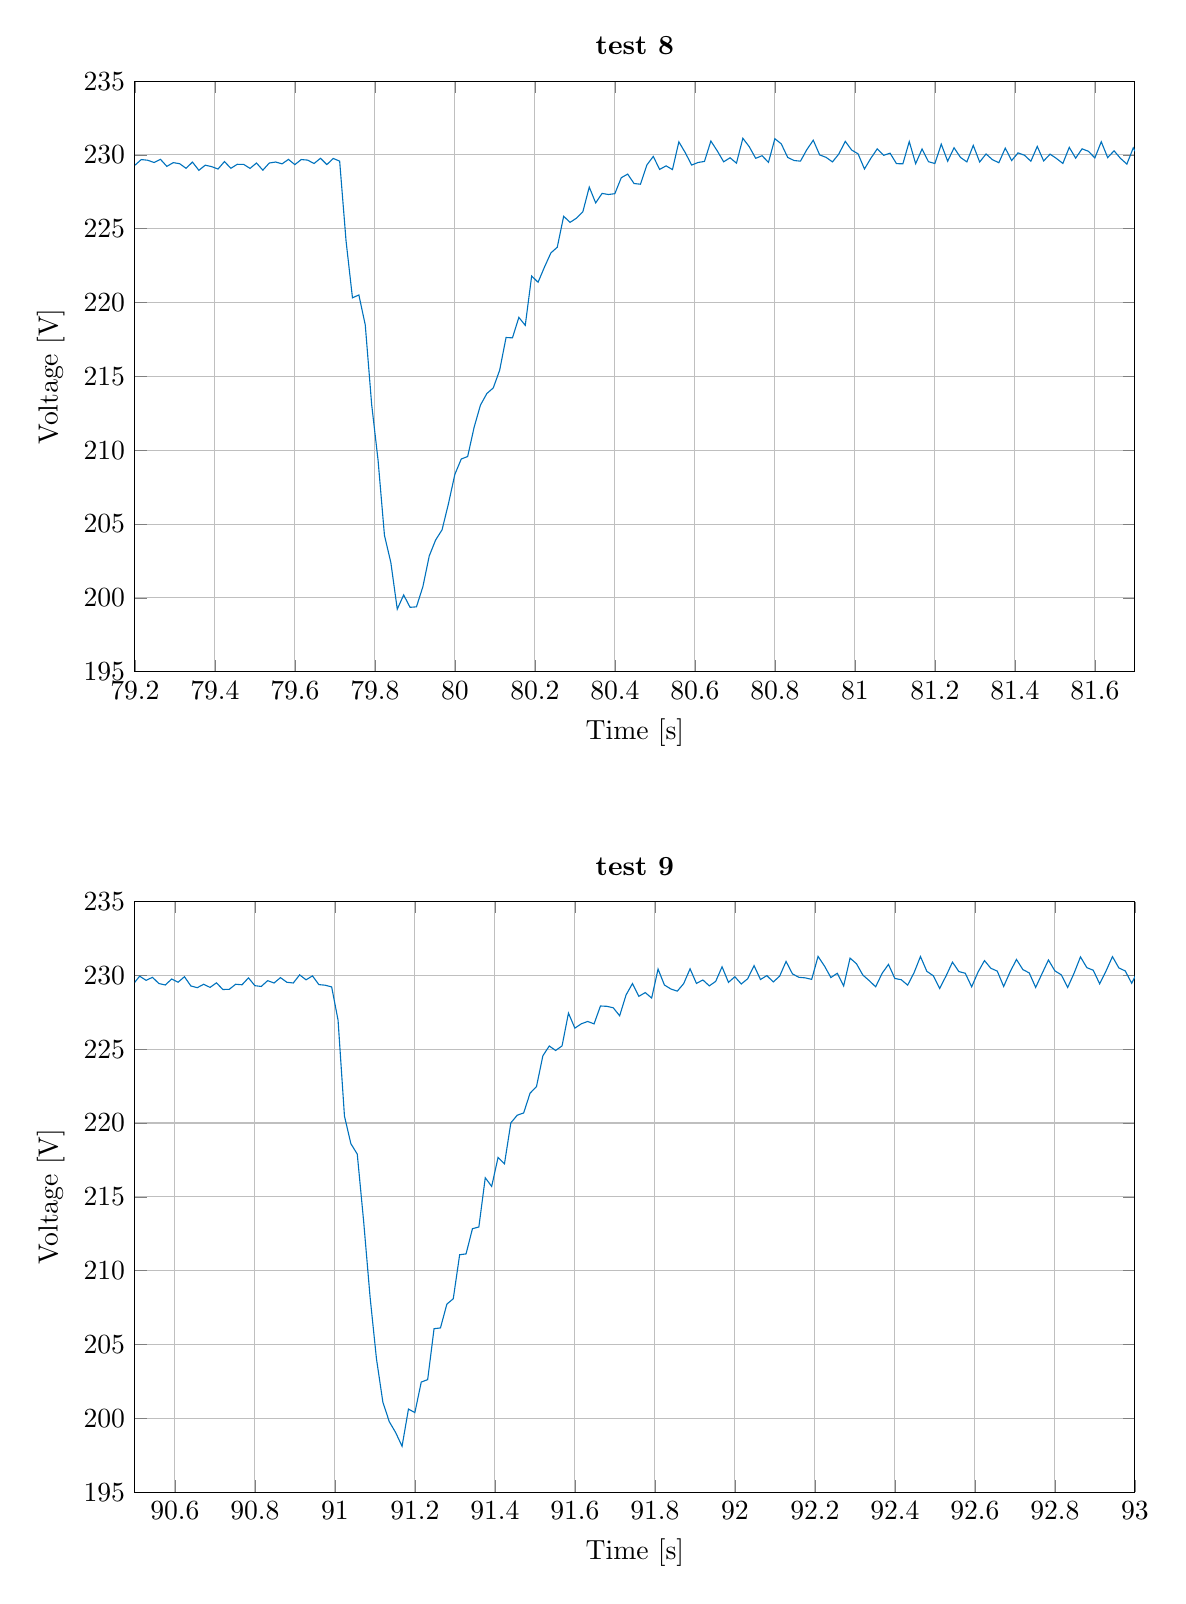
\begin{tikzpicture}

\begin{axis}[%
width=5in,
height=2.953in,
at={(1.142in,5.054in)},
scale only axis,
xmin=79.2,
xmax=81.7,
xlabel={Time [s]},
xmajorgrids,
ymin=195,
ymax=235,
ylabel={Voltage [V]},
ymajorgrids,
axis background/.style={fill=white},
title style={font=\bfseries},
title={test 8}
]
\addplot [color=mycolor1,solid,forget plot]
  table[row sep=crcr]{%
79.2	229.300662365379\\
79.216	229.685879959826\\
79.232	229.640803892063\\
79.248	229.487096203124\\
79.264	229.702745734574\\
79.28	229.224755500342\\
79.296	229.479198058243\\
79.312	229.406058670905\\
79.328	229.094115531369\\
79.344	229.516390349634\\
79.36	228.957990464594\\
79.376	229.305289947812\\
79.392	229.207295866153\\
79.408	229.044698737108\\
79.424	229.552215032356\\
79.44	229.093173481372\\
79.456	229.365444481206\\
79.472	229.360050489918\\
79.488	229.088103707959\\
79.504	229.452881358327\\
79.52	228.968342398354\\
79.536	229.450565800706\\
79.552	229.520700264437\\
79.568	229.396824364227\\
79.584	229.697588662013\\
79.6	229.342446225986\\
79.616	229.687603871069\\
79.632	229.648963970161\\
79.648	229.417109656277\\
79.664	229.775048662789\\
79.68	229.346572272139\\
79.696	229.759771788246\\
79.712	229.579489894458\\
79.728	224.166683275968\\
79.744	220.323078042144\\
79.76	220.51488807548\\
79.776	218.48859294015\\
79.792	213.097056926378\\
79.808	209.326250079888\\
79.824	204.23394924644\\
79.84	202.387616443055\\
79.856	199.236538671744\\
79.872	200.197086581226\\
79.888	199.360223093882\\
79.904	199.393968827004\\
79.92	200.755066487199\\
79.936	202.845008119863\\
79.952	203.922817418315\\
79.968	204.610064217666\\
79.984	206.381584972091\\
80	208.366334458204\\
80.016	209.405680095814\\
80.032	209.573219125046\\
80.048	211.538918643058\\
80.064	213.057416510617\\
80.08	213.841368232295\\
80.096	214.220410909275\\
80.112	215.420471962649\\
80.128	217.635222316228\\
80.144	217.610849862975\\
80.16	218.99947324587\\
80.176	218.456108818699\\
80.192	221.80051097794\\
80.208	221.375582741985\\
80.224	222.40236730584\\
80.24	223.3610991746\\
80.256	223.74865889665\\
80.272	225.845535692629\\
80.288	225.432811742824\\
80.304	225.718600525298\\
80.32	226.153342379993\\
80.336	227.822907559961\\
80.352	226.751880994861\\
80.368	227.392037876646\\
80.384	227.320494139324\\
80.4	227.375033546624\\
80.416	228.456796489274\\
80.432	228.701598887519\\
80.448	228.062682537166\\
80.464	228.017059160967\\
80.48	229.317319154584\\
80.496	229.897751313276\\
80.512	229.017707383381\\
80.528	229.260238715856\\
80.544	229.007378834563\\
80.56	230.88631343687\\
80.576	230.152355869361\\
80.592	229.312388332828\\
80.608	229.487458914991\\
80.624	229.560333976115\\
80.64	230.940951910252\\
80.656	230.275903182037\\
80.672	229.53504801812\\
80.688	229.807115784903\\
80.704	229.442907417126\\
80.72	231.126139595811\\
80.736	230.556559377302\\
80.752	229.77159684046\\
80.768	229.946252628044\\
80.784	229.498929173621\\
80.8	231.097202348574\\
80.816	230.752574673764\\
80.832	229.835511045872\\
80.848	229.621391218738\\
80.864	229.577933725082\\
80.88	230.361899109622\\
80.896	230.996097042733\\
80.912	230.002656532987\\
80.928	229.835385346012\\
80.944	229.526888388817\\
80.96	230.066657994349\\
80.976	230.920500268308\\
80.992	230.330564245024\\
81.008	230.075391148365\\
81.024	229.047961555549\\
81.04	229.772196165414\\
81.056	230.413688202068\\
81.072	229.975050472752\\
81.088	230.120319997252\\
81.104	229.410967305444\\
81.12	229.397806383957\\
81.136	230.903698875236\\
81.152	229.406708330034\\
81.168	230.404927461002\\
81.184	229.543076425023\\
81.2	229.418213861341\\
81.216	230.727655098938\\
81.232	229.573485806519\\
81.248	230.486760115983\\
81.264	229.832110062916\\
81.28	229.528360069307\\
81.296	230.647447510388\\
81.312	229.522640552517\\
81.328	230.065546662592\\
81.344	229.67630268522\\
81.36	229.474037100658\\
81.376	230.461602024439\\
81.392	229.618700123496\\
81.408	230.13860020353\\
81.424	229.979963399801\\
81.44	229.572585611487\\
81.456	230.574480340884\\
81.472	229.593411660184\\
81.488	230.053736566077\\
81.504	229.759861369435\\
81.52	229.42408478484\\
81.536	230.512760294191\\
81.552	229.782015983938\\
81.568	230.414438417279\\
81.584	230.244519625274\\
81.6	229.795719540163\\
81.616	230.893069582097\\
81.632	229.820500759135\\
81.648	230.277381470516\\
81.664	229.769759724742\\
81.68	229.378613875605\\
81.696	230.475798422958\\
81.712	229.701427174059\\
};
\end{axis}

\begin{axis}[%
width=5in,
height=2.953in,
at={(1.142in,0.952in)},
scale only axis,
xmin=90.5,
xmax=93,
xlabel={Time [s]},
xmajorgrids,
ymin=195,
ymax=235,
ylabel={Voltage [V]},
ymajorgrids,
axis background/.style={fill=white},
title style={font=\bfseries},
title={test 9}
]
\addplot [color=mycolor1,solid,forget plot]
  table[row sep=crcr]{%
90.496	229.40001902513\\
90.512	229.946404497269\\
90.528	229.65978204077\\
90.544	229.865755072423\\
90.56	229.445599080904\\
90.576	229.346073780445\\
90.592	229.747360435403\\
90.608	229.530835253204\\
90.624	229.906617679419\\
90.64	229.279885527819\\
90.656	229.1638069099\\
90.672	229.395496865447\\
90.688	229.183143821593\\
90.704	229.492929263405\\
90.72	229.040573721439\\
90.736	229.052151648396\\
90.752	229.395052543857\\
90.768	229.361157538977\\
90.784	229.829769185874\\
90.8	229.299787244518\\
90.816	229.246428263452\\
90.832	229.640102555432\\
90.848	229.480770613746\\
90.864	229.845707054349\\
90.88	229.530562164752\\
90.896	229.480630981366\\
90.912	230.03172235702\\
90.928	229.696031922476\\
90.944	229.96314193775\\
90.96	229.372536572399\\
90.976	229.3297360825\\
90.992	229.215302713319\\
91.008	226.963832541795\\
91.024	220.467235322238\\
91.04	218.598825682068\\
91.056	217.893632860326\\
91.072	213.326297155245\\
91.088	208.227103886479\\
91.104	204.029746437911\\
91.12	201.096966634873\\
91.136	199.774274191778\\
91.152	199.032670428037\\
91.168	198.104092818777\\
91.184	200.623114432456\\
91.2	200.38655290713\\
91.216	202.453276311569\\
91.232	202.616627611329\\
91.248	206.067434869404\\
91.264	206.118550928287\\
91.28	207.731173044932\\
91.296	208.095911625309\\
91.312	211.076481915259\\
91.328	211.132337448481\\
91.344	212.841552608525\\
91.36	212.954757087085\\
91.376	216.28893249289\\
91.392	215.703859310008\\
91.408	217.66918869457\\
91.424	217.233663904765\\
91.44	220.011057934528\\
91.456	220.527568232543\\
91.472	220.679798664899\\
91.488	222.018833700305\\
91.504	222.457964482789\\
91.52	224.551077399255\\
91.536	225.215489801447\\
91.552	224.909784367477\\
91.568	225.222247733354\\
91.584	227.440086605033\\
91.6	226.425127856681\\
91.616	226.71543207285\\
91.632	226.876434546932\\
91.648	226.712485705759\\
91.664	227.923198650111\\
91.68	227.901267664865\\
91.696	227.801327769422\\
91.712	227.261995173327\\
91.728	228.672516254149\\
91.744	229.440877977736\\
91.76	228.578964328346\\
91.776	228.831976224303\\
91.792	228.460707379874\\
91.808	230.423373952154\\
91.824	229.342080393606\\
91.84	229.076036557327\\
91.856	228.927774861029\\
91.872	229.43462176171\\
91.888	230.441727343144\\
91.904	229.451722622811\\
91.92	229.687808425104\\
91.936	229.2875902933\\
91.952	229.585849988952\\
91.968	230.57724134508\\
91.984	229.523963915939\\
92	229.907005279141\\
92.016	229.41383766512\\
92.032	229.766379435536\\
92.048	230.658739401349\\
92.064	229.717094524013\\
92.08	229.981812609017\\
92.096	229.551166494147\\
92.112	229.947441187526\\
92.128	230.939678114845\\
92.144	230.098693983905\\
92.16	229.866347035292\\
92.176	229.828316200853\\
92.192	229.726521002138\\
92.208	231.28235571423\\
92.224	230.634271501089\\
92.24	229.850620005289\\
92.256	230.139554570276\\
92.272	229.284346439451\\
92.288	231.165094235168\\
92.304	230.786993812641\\
92.32	230.017429560391\\
92.336	229.638041689364\\
92.352	229.222835271267\\
92.368	230.131244374888\\
92.384	230.741195520874\\
92.4	229.786939751641\\
92.416	229.702557484902\\
92.432	229.336335627287\\
92.448	230.180943977162\\
92.464	231.273803153628\\
92.48	230.268207922941\\
92.496	229.973835934622\\
92.512	229.110035060332\\
92.528	229.960494038725\\
92.544	230.894756834307\\
92.56	230.254654519607\\
92.576	230.143001370258\\
92.592	229.223141716534\\
92.608	230.223714853964\\
92.624	230.997450145944\\
92.64	230.478235555569\\
92.656	230.286036774805\\
92.672	229.245616615885\\
92.688	230.225441803379\\
92.704	231.075969730301\\
92.72	230.389768167954\\
92.736	230.162636730316\\
92.752	229.179806863289\\
92.768	230.119651996722\\
92.784	231.039576262448\\
92.8	230.304168090122\\
92.816	230.036613614327\\
92.832	229.178790923111\\
92.848	230.143438081877\\
92.864	231.248432170302\\
92.88	230.517644622922\\
92.896	230.344285058519\\
92.912	229.42374899851\\
92.928	230.299472378688\\
92.944	231.266137878868\\
92.96	230.500319107604\\
92.976	230.297150098387\\
92.992	229.465242216764\\
93.008	230.316296197003\\
};
\end{axis}
\end{tikzpicture}%
\caption{Voltage disturbance on the output of the genset occuring from step of 10 to 50 kW load.}
\label{fig:test8-9-10to50kwstepvolt}
\end{figure}

\begin{figure}[H]
\centering
% This file was created by matlab2tikz.
%
%The latest updates can be retrieved from
%  http://www.mathworks.com/matlabcentral/fileexchange/22022-matlab2tikz-matlab2tikz
%where you can also make suggestions and rate matlab2tikz.
%
\definecolor{mycolor1}{rgb}{0.00000,0.44700,0.74100}%
%
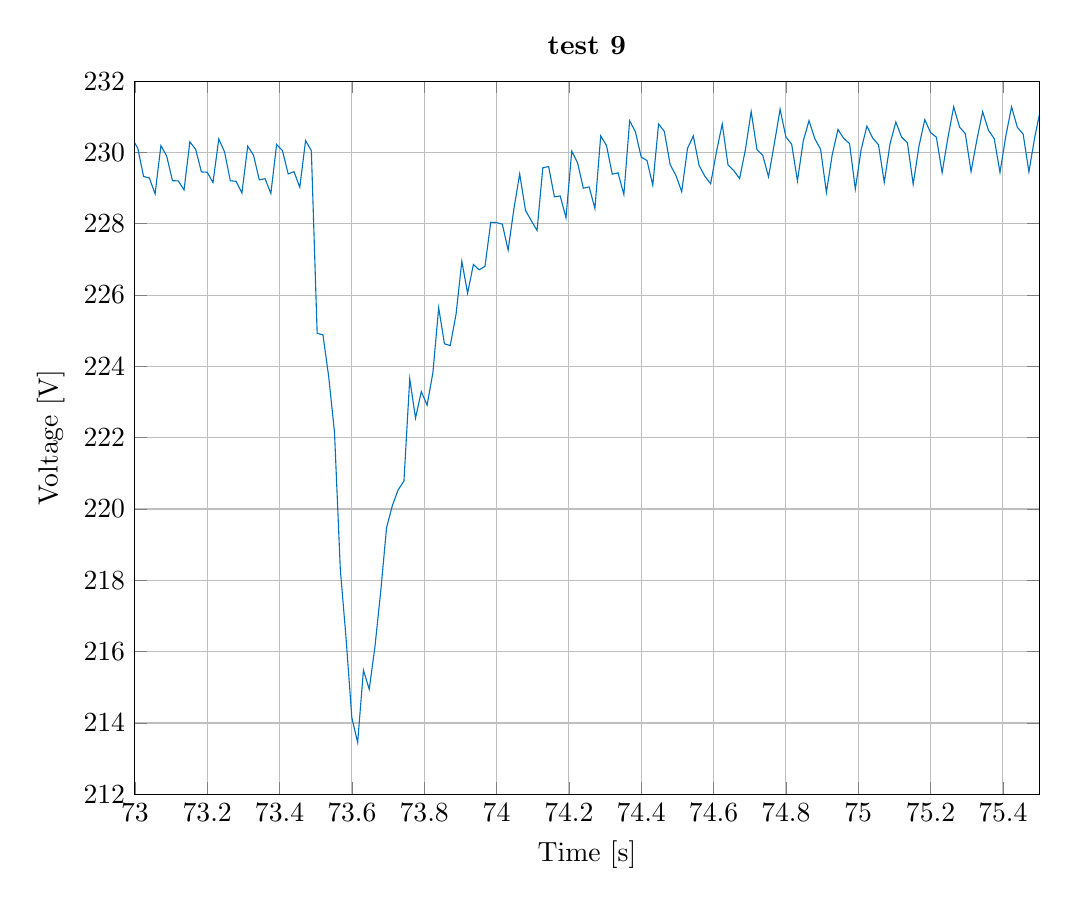
\begin{tikzpicture}

\begin{axis}[%
width=4.521in,
height=3.566in,
at={(0.758in,0.481in)},
scale only axis,
xmin=73,
xmax=75.5,
xlabel={Time [s]},
xmajorgrids,
ymin=212,
ymax=232,
ylabel={Voltage [V]},
ymajorgrids,
axis background/.style={fill=white},
title style={font=\bfseries},
title={test 9}
]
\addplot [color=mycolor1,solid,forget plot]
  table[row sep=crcr]{%
72.992	230.393376163564\\
73.008	230.122711104588\\
73.024	229.32669588555\\
73.04	229.28359794795\\
73.056	228.838345280919\\
73.072	230.190174716611\\
73.088	229.898515675003\\
73.104	229.207263947965\\
73.12	229.201674152063\\
73.136	228.948915097948\\
73.152	230.296619278984\\
73.168	230.08881782874\\
73.184	229.453138212141\\
73.2	229.444093312475\\
73.216	229.155685405403\\
73.232	230.376452082391\\
73.248	230.013379885466\\
73.264	229.204587928961\\
73.28	229.191130669724\\
73.296	228.860855786359\\
73.312	230.175864677182\\
73.328	229.923686447189\\
73.344	229.230986754771\\
73.36	229.263432155825\\
73.376	228.849919378081\\
73.392	230.224161775455\\
73.408	230.049839928295\\
73.424	229.396134633259\\
73.44	229.46076093928\\
73.456	229.022353725253\\
73.472	230.332048044231\\
73.488	230.044800858342\\
73.504	224.927464866499\\
73.52	224.884408046764\\
73.536	223.708141657088\\
73.552	222.150425952761\\
73.568	218.319040510205\\
73.584	216.367267852313\\
73.6	214.142191220624\\
73.616	213.45414158124\\
73.632	215.481599635026\\
73.648	214.943962274523\\
73.664	216.156653048496\\
73.68	217.714350719931\\
73.696	219.483393034807\\
73.712	220.09971972839\\
73.728	220.538829145089\\
73.744	220.785494294441\\
73.76	223.652883684255\\
73.776	222.549512701348\\
73.792	223.294810542244\\
73.808	222.913222087754\\
73.824	223.820715570985\\
73.84	225.643438156403\\
73.856	224.63367947825\\
73.872	224.584266291371\\
73.888	225.460061795461\\
73.904	226.94569283837\\
73.92	226.053793958853\\
73.936	226.857429647326\\
73.952	226.707516503023\\
73.968	226.805008610069\\
73.984	228.041515910127\\
74	228.032471137731\\
74.016	227.988679854463\\
74.032	227.262058833554\\
74.048	228.417974546237\\
74.064	229.396217137657\\
74.08	228.375501369798\\
74.096	228.089621376475\\
74.112	227.812931750345\\
74.128	229.571167371314\\
74.144	229.603968903817\\
74.16	228.75540989717\\
74.176	228.778409543466\\
74.192	228.170867329695\\
74.208	230.035451065626\\
74.224	229.708520288519\\
74.24	228.995705098649\\
74.256	229.032848203688\\
74.272	228.426996998871\\
74.288	230.464016701156\\
74.304	230.192636471474\\
74.32	229.389417232355\\
74.336	229.427555803702\\
74.352	228.818286648045\\
74.368	230.885415357166\\
74.384	230.578455319941\\
74.4	229.868225199485\\
74.416	229.773494103444\\
74.432	229.081130426162\\
74.448	230.797996559674\\
74.464	230.586221990946\\
74.48	229.657636146794\\
74.496	229.355147536449\\
74.512	228.899153317311\\
74.528	230.11103769607\\
74.544	230.462074470061\\
74.56	229.635967512085\\
74.576	229.33198245862\\
74.592	229.12147368663\\
74.608	230.012861474451\\
74.624	230.798413100685\\
74.64	229.649799517389\\
74.656	229.48960039651\\
74.672	229.267922469634\\
74.688	230.072589326534\\
74.704	231.148225361562\\
74.72	230.079237618721\\
74.736	229.917527667097\\
74.752	229.316956316027\\
74.768	230.243283290517\\
74.784	231.210917774583\\
74.8	230.433552595982\\
74.816	230.230845258927\\
74.832	229.200564423381\\
74.848	230.319684633485\\
74.864	230.891909937665\\
74.88	230.381717349468\\
74.896	230.090557432683\\
74.912	228.877919126924\\
74.928	229.930966580965\\
74.944	230.642754149411\\
74.96	230.391440279167\\
74.976	230.24795987615\\
74.992	228.971676624395\\
75.008	230.078045970866\\
75.024	230.737602641094\\
75.04	230.401597889948\\
75.056	230.217079321704\\
75.072	229.162176788311\\
75.088	230.245276388448\\
75.104	230.853014455471\\
75.12	230.428082286994\\
75.136	230.269202984386\\
75.152	229.107948015509\\
75.168	230.176582915287\\
75.184	230.919174420651\\
75.2	230.558323167603\\
75.216	230.427642295646\\
75.232	229.433506747334\\
75.248	230.411720880236\\
75.264	231.280471589747\\
75.28	230.713818191822\\
75.296	230.528249680349\\
75.312	229.46370527109\\
75.328	230.350205949623\\
75.344	231.14160536173\\
75.36	230.623012777186\\
75.376	230.387508263729\\
75.392	229.438844491568\\
75.408	230.455462683638\\
75.424	231.279432096849\\
75.44	230.70376674217\\
75.456	230.512425722198\\
75.472	229.45313396447\\
75.488	230.422517721141\\
75.504	231.209920498695\\
};
\end{axis}
\end{tikzpicture}%
\caption{Voltage disturbance on the output of the genset occuring from step of 30 to 50 kW load.}
\label{fig:test9-30to50kwstepvolt}
\end{figure}

\begin{figure}[H]
\centering
% This file was created by matlab2tikz.
%
%The latest updates can be retrieved from
%  http://www.mathworks.com/matlabcentral/fileexchange/22022-matlab2tikz-matlab2tikz
%where you can also make suggestions and rate matlab2tikz.
%
\definecolor{mycolor1}{rgb}{0.00000,0.44700,0.74100}%
%
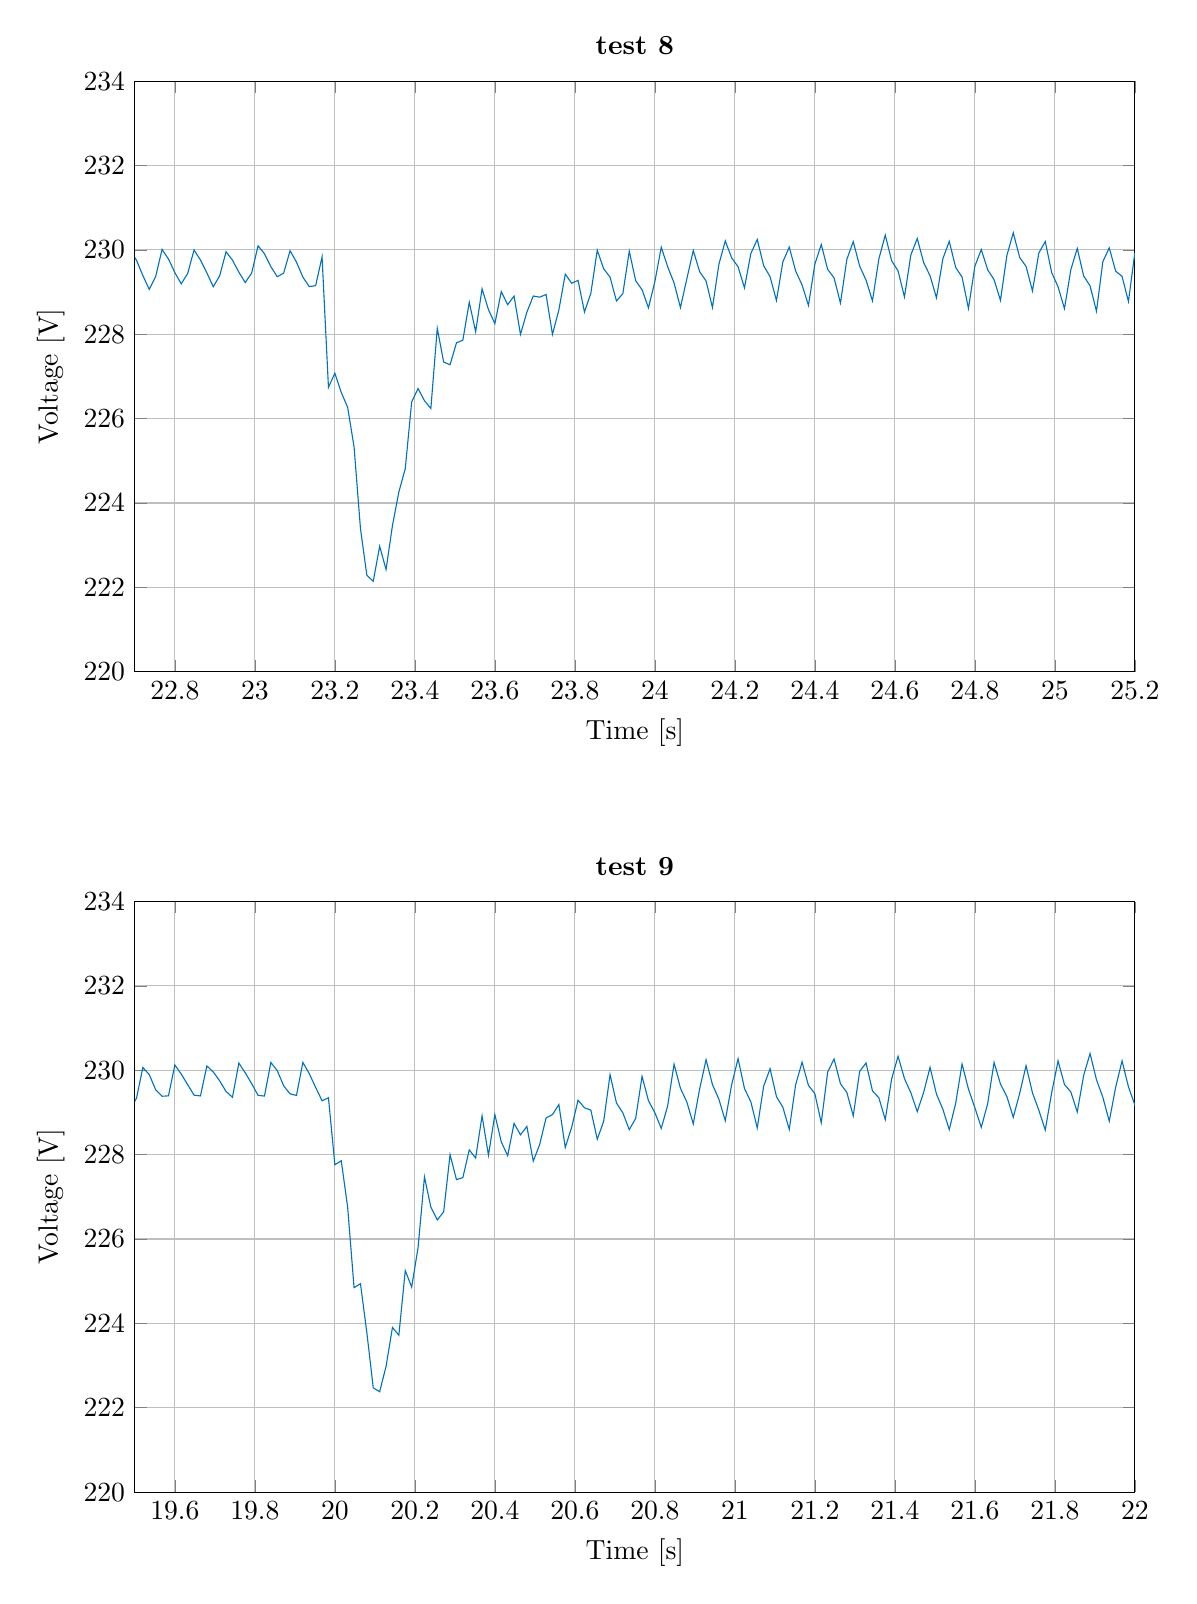
\begin{tikzpicture}

\begin{axis}[%
width=5in,
height=2.953in,
at={(1.142in,5.054in)},
scale only axis,
xmin=22.7,
xmax=25.2,
xlabel={Time [s]},
xmajorgrids,
ymin=220,
ymax=234,
ylabel={Voltage [V]},
ymajorgrids,
axis background/.style={fill=white},
title style={font=\bfseries},
title={test 8}
]
\addplot [color=mycolor1,solid,forget plot]
  table[row sep=crcr]{%
22.688	229.985173537134\\
22.704	229.755318920515\\
22.72	229.391086306003\\
22.736	229.061197123596\\
22.752	229.365101671121\\
22.768	230.011535543695\\
22.784	229.78433670103\\
22.8	229.459418407522\\
22.816	229.194499736557\\
22.832	229.439490935963\\
22.848	229.998152282658\\
22.864	229.759008327834\\
22.88	229.453105950486\\
22.896	229.12665921109\\
22.912	229.383571980158\\
22.928	229.95528632413\\
22.944	229.755793228974\\
22.96	229.471176350049\\
22.976	229.223916811137\\
22.992	229.450675310923\\
23.008	230.095133045459\\
23.024	229.908738814126\\
23.04	229.601377967914\\
23.056	229.362692002392\\
23.072	229.447839011785\\
23.088	229.979719521194\\
23.104	229.709497238476\\
23.12	229.35447493813\\
23.136	229.129044012428\\
23.152	229.151018521351\\
23.168	229.835229873847\\
23.184	226.739456710433\\
23.2	227.076652901712\\
23.216	226.621736785808\\
23.232	226.267135392901\\
23.248	225.331035521847\\
23.264	223.392136305783\\
23.28	222.285649841967\\
23.296	222.143981201873\\
23.312	222.972574249643\\
23.328	222.423906218219\\
23.344	223.465708954518\\
23.36	224.261390871722\\
23.376	224.811410086885\\
23.392	226.39378987966\\
23.408	226.711368418361\\
23.424	226.425221308128\\
23.44	226.240385743222\\
23.456	228.141464294356\\
23.472	227.340281442321\\
23.488	227.27651231268\\
23.504	227.795544408403\\
23.52	227.859997296007\\
23.536	228.759392523974\\
23.552	228.05813240013\\
23.568	229.076055509652\\
23.584	228.581911683237\\
23.6	228.250240475284\\
23.616	229.009836870942\\
23.632	228.700243731579\\
23.648	228.905071515245\\
23.664	227.996712525699\\
23.68	228.520954672748\\
23.696	228.905408835514\\
23.712	228.878605539116\\
23.728	228.941630373706\\
23.744	227.99589017644\\
23.76	228.574544995099\\
23.776	229.424321372088\\
23.792	229.209562164554\\
23.808	229.275315688313\\
23.824	228.526334060035\\
23.84	228.972585818592\\
23.856	229.992668916109\\
23.872	229.552908623312\\
23.888	229.352421759234\\
23.904	228.788025526098\\
23.92	228.961862509787\\
23.936	229.968964958511\\
23.952	229.26993568248\\
23.968	229.053001927011\\
23.984	228.627036490637\\
24	229.245265921995\\
24.016	230.063177722537\\
24.032	229.599759201865\\
24.048	229.215392681505\\
24.064	228.63317962675\\
24.08	229.316909651675\\
24.096	229.984674859096\\
24.112	229.481345336619\\
24.128	229.262980942599\\
24.144	228.632891151849\\
24.16	229.654450646327\\
24.176	230.211952810946\\
24.192	229.808758139791\\
24.208	229.600333375737\\
24.224	229.099669125591\\
24.24	229.914271820836\\
24.256	230.245498948148\\
24.272	229.624515241211\\
24.288	229.36378459628\\
24.304	228.799285275565\\
24.32	229.715668006143\\
24.336	230.064822815609\\
24.352	229.497208474902\\
24.368	229.166641486987\\
24.384	228.682880836958\\
24.4	229.660663396228\\
24.416	230.127240550322\\
24.432	229.537017288117\\
24.448	229.336196342122\\
24.464	228.738103493305\\
24.48	229.77533622273\\
24.496	230.194386247114\\
24.512	229.614321774269\\
24.528	229.281738179364\\
24.544	228.789853134609\\
24.56	229.784109608172\\
24.576	230.349825994116\\
24.592	229.739693032621\\
24.608	229.501680617981\\
24.624	228.883594559245\\
24.64	229.880357174041\\
24.656	230.269234415649\\
24.672	229.694756301554\\
24.688	229.38761371397\\
24.704	228.863060592665\\
24.72	229.7885292486\\
24.736	230.201317784605\\
24.752	229.58338864003\\
24.768	229.355882957416\\
24.784	228.610851691358\\
24.8	229.610917260346\\
24.816	230.007230149982\\
24.832	229.528222362182\\
24.848	229.292868744226\\
24.864	228.802975851939\\
24.88	229.863670229343\\
24.896	230.404225249665\\
24.912	229.82011088978\\
24.928	229.606750796352\\
24.944	229.026146908659\\
24.96	229.926721648429\\
24.976	230.196504086922\\
24.992	229.462143472648\\
25.008	229.124638993524\\
25.024	228.607791658258\\
25.04	229.531384440665\\
25.056	230.034002237939\\
25.072	229.37898902935\\
25.088	229.147790159789\\
25.104	228.545262801536\\
25.12	229.721537484445\\
25.136	230.046832867409\\
25.152	229.495376979801\\
25.168	229.371078085441\\
25.184	228.775049833452\\
25.2	229.934442615864\\
25.2	229.934442615864\\
};
\end{axis}

\begin{axis}[%
width=5in,
height=2.953in,
at={(1.142in,0.952in)},
scale only axis,
xmin=19.5,
xmax=22,
xlabel={Time [s]},
xmajorgrids,
ymin=220,
ymax=234,
ylabel={Voltage [V]},
ymajorgrids,
axis background/.style={fill=white},
title style={font=\bfseries},
title={test 9}
]
\addplot [color=mycolor1,solid,forget plot]
  table[row sep=crcr]{%
19.488	229.069920654615\\
19.504	229.33372521576\\
19.52	230.06514324614\\
19.536	229.897369487197\\
19.552	229.536006886058\\
19.568	229.383728874208\\
19.584	229.393354525184\\
19.6	230.125416078628\\
19.616	229.908924273916\\
19.632	229.658914921739\\
19.648	229.409617079333\\
19.664	229.391259026269\\
19.68	230.102466621561\\
19.696	229.960214181554\\
19.712	229.749552635651\\
19.728	229.496415703656\\
19.744	229.360656837482\\
19.76	230.16861848815\\
19.776	229.939310900804\\
19.792	229.682347927539\\
19.808	229.404833465599\\
19.824	229.388522567473\\
19.84	230.18421458013\\
19.856	229.991790001559\\
19.872	229.630158943837\\
19.888	229.441098642269\\
19.904	229.403378306477\\
19.92	230.185999540126\\
19.936	229.920341386045\\
19.952	229.592040407181\\
19.968	229.276651574678\\
19.984	229.348572863916\\
20	227.759416526836\\
20.016	227.85494067972\\
20.032	226.752504349333\\
20.048	224.846584729221\\
20.064	224.940836904541\\
20.08	223.777541864043\\
20.096	222.471406263342\\
20.112	222.37987498579\\
20.128	222.981896192199\\
20.144	223.903142720349\\
20.16	223.718183581616\\
20.176	225.250495017587\\
20.192	224.86071852923\\
20.208	225.796978581855\\
20.224	227.470114021787\\
20.24	226.754510051572\\
20.256	226.451487848465\\
20.272	226.643453516162\\
20.288	227.99868137347\\
20.304	227.408218100173\\
20.32	227.455275231168\\
20.336	228.112706337209\\
20.352	227.918545319153\\
20.368	228.920229825869\\
20.384	227.984714515952\\
20.4	228.95033834876\\
20.416	228.303606516139\\
20.432	227.974795250795\\
20.448	228.739609170838\\
20.464	228.469001567075\\
20.48	228.669415626242\\
20.496	227.844929879034\\
20.512	228.239307602771\\
20.528	228.868969466419\\
20.544	228.949464542564\\
20.56	229.186544824275\\
20.576	228.168090600283\\
20.592	228.648775620592\\
20.608	229.290126839676\\
20.624	229.110448187389\\
20.64	229.054494768427\\
20.656	228.364215311246\\
20.672	228.788233352918\\
20.688	229.897043102718\\
20.704	229.223926302149\\
20.72	228.988808237642\\
20.736	228.591951327356\\
20.752	228.855994004434\\
20.768	229.856641861004\\
20.784	229.277801565089\\
20.8	228.992092225162\\
20.816	228.621034410402\\
20.832	229.155648294293\\
20.848	230.144105091504\\
20.864	229.572085856266\\
20.88	229.245567824\\
20.896	228.728664897674\\
20.912	229.55956578043\\
20.928	230.250798097056\\
20.944	229.660404806921\\
20.96	229.315951454318\\
20.976	228.804624457392\\
20.992	229.658557869477\\
21.008	230.274643891468\\
21.024	229.568821191437\\
21.04	229.250504103683\\
21.056	228.632958184811\\
21.072	229.622772372686\\
21.088	230.035976116753\\
21.104	229.374255992523\\
21.12	229.123238451074\\
21.136	228.597986352854\\
21.152	229.660187616888\\
21.168	230.190087153875\\
21.184	229.640200627399\\
21.2	229.445080272065\\
21.216	228.755907131147\\
21.232	229.957091126554\\
21.248	230.26660324816\\
21.264	229.680364324647\\
21.28	229.471359593893\\
21.296	228.919872949752\\
21.312	229.974253346484\\
21.328	230.172025157937\\
21.344	229.510524737288\\
21.36	229.347609096079\\
21.376	228.830043750042\\
21.392	229.797299513983\\
21.408	230.331839668586\\
21.424	229.8015205084\\
21.44	229.464762289688\\
21.456	229.020284503974\\
21.472	229.478391807015\\
21.488	230.069008424827\\
21.504	229.434556834655\\
21.52	229.076118114845\\
21.536	228.592545788169\\
21.552	229.216952584218\\
21.568	230.147785103315\\
21.584	229.55312194845\\
21.6	229.110823357608\\
21.616	228.64680128155\\
21.632	229.206672938651\\
21.648	230.18513803675\\
21.664	229.673501323967\\
21.68	229.377191482465\\
21.696	228.883157822242\\
21.712	229.451238818019\\
21.728	230.107533231888\\
21.744	229.465184357839\\
21.76	229.050737475577\\
21.776	228.583114991434\\
21.792	229.467419493757\\
21.808	230.220326335081\\
21.824	229.662424037036\\
21.84	229.484698366507\\
21.856	229.011668948898\\
21.872	229.877692941873\\
21.888	230.39580840452\\
21.904	229.776739100143\\
21.92	229.358304894223\\
21.936	228.792343573169\\
21.952	229.598759738096\\
21.968	230.223653507692\\
21.984	229.606142150327\\
22	229.178506955685\\
22.016	228.677671920372\\
};
\end{axis}
\end{tikzpicture}%
\caption{Voltage disturbance on the output of the genset occuring from step of 20 to 30 kW load.}
\label{fig:test8-9-20to30kwstepvolt}
\end{figure}

\begin{figure}[H]
\centering
% This file was created by matlab2tikz.
%
%The latest updates can be retrieved from
%  http://www.mathworks.com/matlabcentral/fileexchange/22022-matlab2tikz-matlab2tikz
%where you can also make suggestions and rate matlab2tikz.
%
\definecolor{mycolor1}{rgb}{0.00000,0.44700,0.74100}%
%
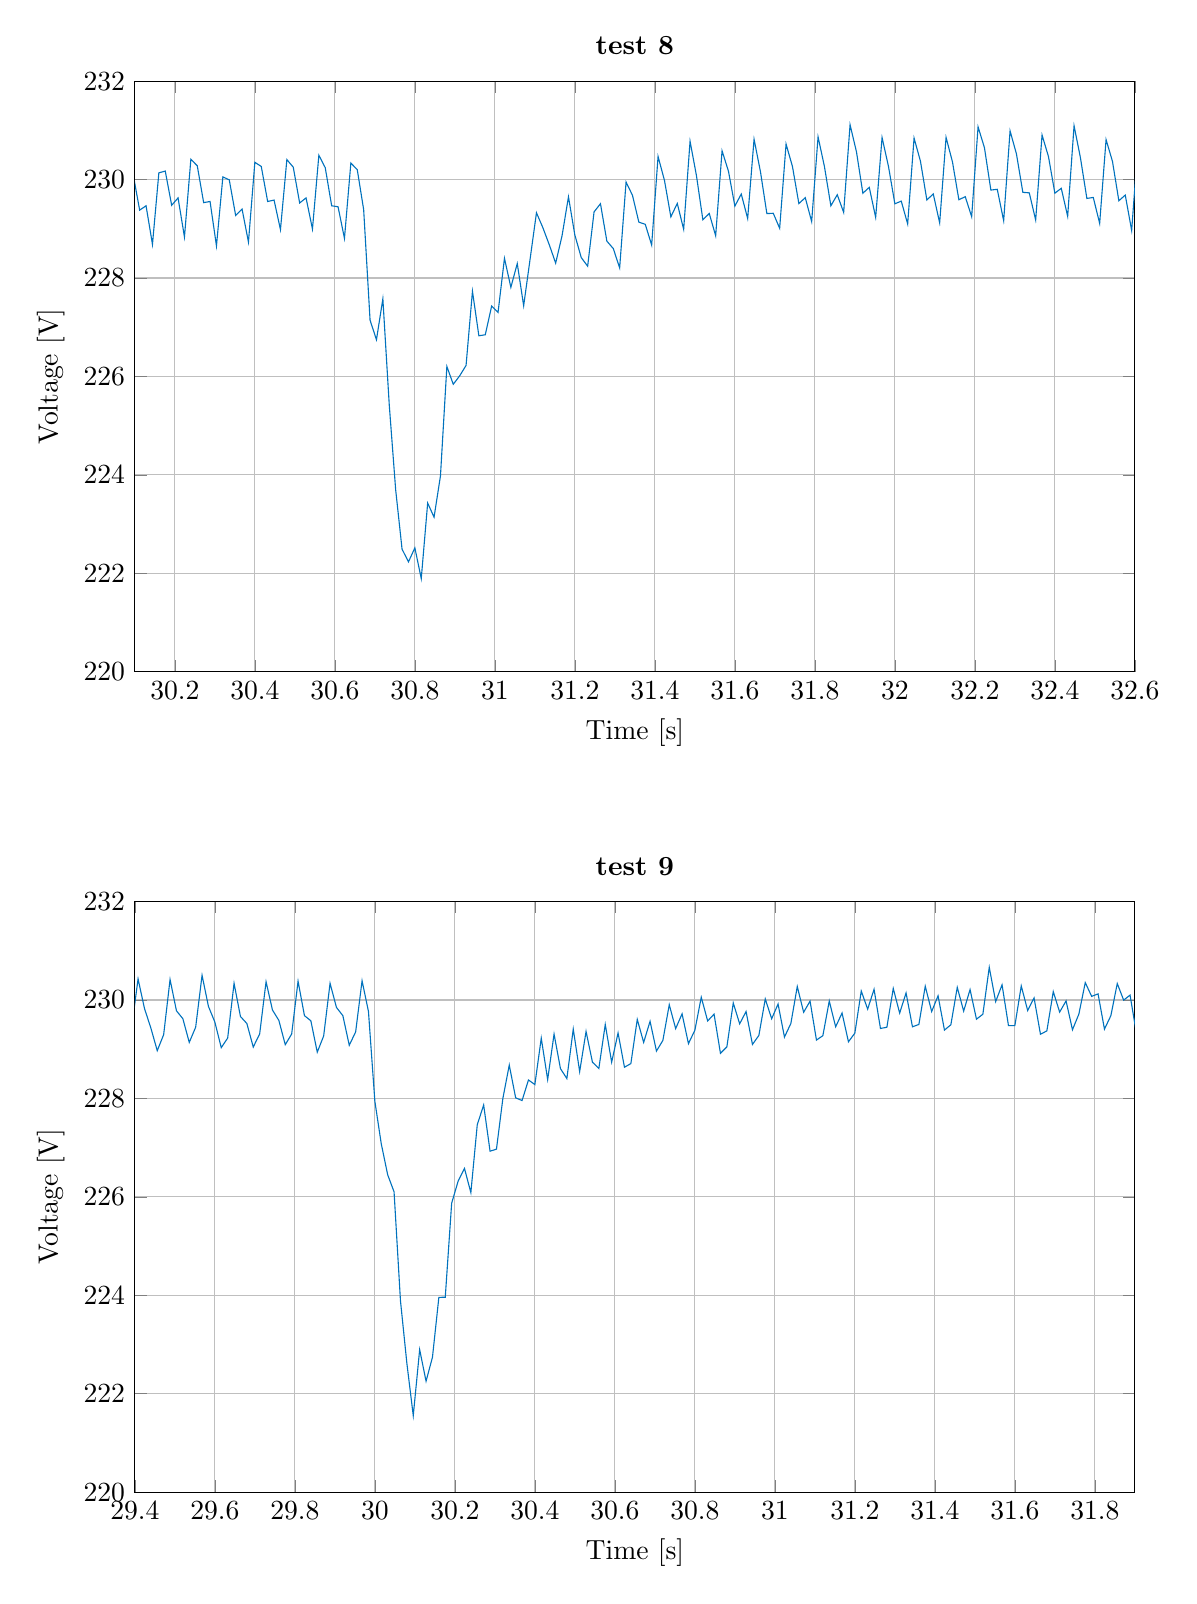
\begin{tikzpicture}

\begin{axis}[%
width=5in,
height=2.953in,
at={(1.142in,5.054in)},
scale only axis,
xmin=30.1,
xmax=32.6,
xlabel={Time [s]},
xmajorgrids,
ymin=220,
ymax=232,
ylabel={Voltage [V]},
ymajorgrids,
axis background/.style={fill=white},
title style={font=\bfseries},
title={test 8}
]
\addplot [color=mycolor1,solid,forget plot]
  table[row sep=crcr]{%
30.096	230.092385731796\\
30.112	229.378080662134\\
30.128	229.467096288622\\
30.144	228.681991448146\\
30.16	230.135845423164\\
30.176	230.172209172349\\
30.192	229.476941403285\\
30.208	229.626820744654\\
30.224	228.832220708436\\
30.24	230.412584349082\\
30.256	230.279404206535\\
30.272	229.531042742327\\
30.288	229.553979593962\\
30.304	228.651886107534\\
30.32	230.05357361655\\
30.336	229.993669904286\\
30.352	229.270476704834\\
30.368	229.40003416493\\
30.384	228.729238250473\\
30.4	230.35053326485\\
30.416	230.2654273441\\
30.432	229.553999729631\\
30.448	229.582891931627\\
30.464	228.982381676217\\
30.48	230.405511036624\\
30.496	230.250499041306\\
30.512	229.524127922526\\
30.528	229.626745259629\\
30.544	228.994109740708\\
30.56	230.493554570247\\
30.576	230.239365382339\\
30.592	229.467019636074\\
30.608	229.445985334137\\
30.624	228.804098161708\\
30.64	230.335867372133\\
30.656	230.199655200381\\
30.672	229.388701296818\\
30.688	227.143107224995\\
30.704	226.745300127748\\
30.72	227.576269305694\\
30.736	225.420274520019\\
30.752	223.697493867594\\
30.768	222.490069816341\\
30.784	222.23215568522\\
30.8	222.516009271008\\
30.816	221.892694361707\\
30.832	223.42601611976\\
30.848	223.140260487021\\
30.864	223.97797669063\\
30.88	226.201423481396\\
30.896	225.840131186253\\
30.912	226.010870122005\\
30.928	226.223263065195\\
30.944	227.730295027672\\
30.96	226.825629484651\\
30.976	226.845952954025\\
30.992	227.429713465462\\
31.008	227.302183477153\\
31.024	228.399174713349\\
31.04	227.809761179058\\
31.056	228.293164135935\\
31.072	227.435853723954\\
31.088	228.378112026771\\
31.104	229.324913533539\\
31.12	229.022295324092\\
31.136	228.675827718037\\
31.152	228.301557791796\\
31.168	228.859011578407\\
31.184	229.647944864702\\
31.2	228.870892118427\\
31.216	228.414113504177\\
31.232	228.240002640459\\
31.248	229.342065739726\\
31.264	229.50898971969\\
31.28	228.748154232615\\
31.296	228.598247239957\\
31.312	228.207246379709\\
31.328	229.948140023373\\
31.344	229.680095369508\\
31.36	229.133530480935\\
31.376	229.090460678273\\
31.392	228.6682992077\\
31.408	230.468545865262\\
31.424	229.982792698532\\
31.44	229.241651626479\\
31.456	229.51381474684\\
31.472	228.989696398494\\
31.488	230.778040004072\\
31.504	230.078138973001\\
31.52	229.182933089854\\
31.536	229.309792148912\\
31.552	228.857969765669\\
31.568	230.583783080977\\
31.584	230.16908661079\\
31.6	229.460609516256\\
31.616	229.7051272413\\
31.632	229.20859636961\\
31.648	230.818432365109\\
31.664	230.159337092542\\
31.68	229.308198756217\\
31.696	229.314529154426\\
31.712	229.010088309026\\
31.728	230.71987923814\\
31.744	230.264891285615\\
31.76	229.51171883036\\
31.776	229.631029309893\\
31.792	229.145547910893\\
31.808	230.866906138655\\
31.824	230.261936011243\\
31.84	229.466290902364\\
31.856	229.690678833023\\
31.872	229.332389862263\\
31.888	231.112635716361\\
31.904	230.564099354654\\
31.92	229.721927592725\\
31.936	229.841845754877\\
31.952	229.23132739793\\
31.968	230.852632850027\\
31.984	230.269282635281\\
32	229.507324809836\\
32.016	229.561473486473\\
32.032	229.097425673036\\
32.048	230.842246710692\\
32.064	230.372239174047\\
32.08	229.585297527207\\
32.096	229.706898712043\\
32.112	229.119661821145\\
32.128	230.856137244166\\
32.144	230.358967351133\\
32.16	229.590155569482\\
32.176	229.650993472035\\
32.192	229.244573421722\\
32.208	231.070529523768\\
32.224	230.645481981368\\
32.24	229.786372951373\\
32.256	229.801314302602\\
32.272	229.163535029118\\
32.288	230.988523814323\\
32.304	230.518844458954\\
32.32	229.739980300256\\
32.336	229.729511851887\\
32.352	229.178222307581\\
32.368	230.904257980709\\
32.384	230.467505074953\\
32.4	229.722435928666\\
32.416	229.822242629718\\
32.432	229.252952119771\\
32.448	231.093437847172\\
32.464	230.439339594977\\
32.48	229.61616540904\\
32.496	229.636310180681\\
32.512	229.108718604408\\
32.528	230.811220297232\\
32.544	230.369209876657\\
32.56	229.569076794687\\
32.576	229.684339271838\\
32.592	228.965255834394\\
32.608	230.729725057307\\
};
\end{axis}

\begin{axis}[%
width=5in,
height=2.953in,
at={(1.142in,0.952in)},
scale only axis,
xmin=29.4,
xmax=31.9,
xlabel={Time [s]},
xmajorgrids,
ymin=220,
ymax=232,
ylabel={Voltage [V]},
ymajorgrids,
axis background/.style={fill=white},
title style={font=\bfseries},
title={test 9}
]
\addplot [color=mycolor1,solid,forget plot]
  table[row sep=crcr]{%
29.392	229.443796618885\\
29.408	230.426810635472\\
29.424	229.828597113987\\
29.44	229.428916443887\\
29.456	228.969145475214\\
29.472	229.294816048476\\
29.488	230.415510498302\\
29.504	229.779042165368\\
29.52	229.618886919587\\
29.536	229.137650542053\\
29.552	229.445672716902\\
29.568	230.500203701383\\
29.584	229.86815318059\\
29.6	229.550412751654\\
29.616	229.030868387836\\
29.632	229.223888230525\\
29.648	230.337741763721\\
29.664	229.663436815051\\
29.68	229.521317391225\\
29.696	229.042685835345\\
29.712	229.308989733659\\
29.728	230.370116760873\\
29.744	229.795526430044\\
29.76	229.584417017999\\
29.776	229.091549739817\\
29.792	229.307204167662\\
29.808	230.380695713214\\
29.824	229.680867220302\\
29.84	229.576244213411\\
29.856	228.938552575818\\
29.872	229.268140166352\\
29.888	230.338055793315\\
29.904	229.847528607316\\
29.92	229.680868631265\\
29.936	229.078827082758\\
29.952	229.350882071998\\
29.968	230.389892486672\\
29.984	229.766323142421\\
30	227.940342777403\\
30.016	227.077343871109\\
30.032	226.448885985575\\
30.048	226.101118212574\\
30.064	223.89038508622\\
30.08	222.618877846572\\
30.096	221.553547155905\\
30.112	222.894877544843\\
30.128	222.253164694128\\
30.144	222.740413234484\\
30.16	223.956827886208\\
30.176	223.95988798573\\
30.192	225.870126478977\\
30.208	226.313808668672\\
30.224	226.577720414241\\
30.24	226.084982809343\\
30.256	227.464502226936\\
30.272	227.865417881188\\
30.288	226.926771919693\\
30.304	226.968322749942\\
30.32	227.998381213178\\
30.336	228.675881093556\\
30.352	228.011014740125\\
30.368	227.956153643949\\
30.384	228.373288585112\\
30.4	228.280399018579\\
30.416	229.223239204745\\
30.432	228.381466145794\\
30.448	229.306237835026\\
30.464	228.604478252589\\
30.48	228.40290363478\\
30.496	229.407794941672\\
30.512	228.543303573872\\
30.528	229.359545181256\\
30.544	228.734783903379\\
30.56	228.609778928685\\
30.576	229.501395610517\\
30.592	228.735758669909\\
30.608	229.329653427586\\
30.624	228.633311872326\\
30.64	228.7064659503\\
30.656	229.604570571857\\
30.672	229.13715653961\\
30.688	229.565954947215\\
30.704	228.961999926574\\
30.72	229.176603045242\\
30.736	229.902737871327\\
30.752	229.417512804737\\
30.768	229.717399080254\\
30.784	229.112052528436\\
30.8	229.38364471736\\
30.816	230.05513811187\\
30.832	229.57325060019\\
30.848	229.71103024864\\
30.864	228.915725295709\\
30.88	229.046234882522\\
30.896	229.938038432606\\
30.912	229.514415516445\\
30.928	229.764362964273\\
30.944	229.096638181729\\
30.96	229.278443092057\\
30.976	230.020122929191\\
30.992	229.617831483728\\
31.008	229.917177088066\\
31.024	229.24610821638\\
31.04	229.521425759861\\
31.056	230.271647039597\\
31.072	229.750147327924\\
31.088	229.97596108752\\
31.104	229.184680435679\\
31.12	229.274136488534\\
31.136	229.977420511054\\
31.152	229.455244173909\\
31.168	229.734254425564\\
31.184	229.149420379363\\
31.2	229.326390212345\\
31.216	230.18097980785\\
31.232	229.813301912029\\
31.248	230.216429032647\\
31.264	229.42058777267\\
31.28	229.44543913978\\
31.296	230.232675938242\\
31.312	229.732812551798\\
31.328	230.142250754066\\
31.344	229.454305072978\\
31.36	229.501814159256\\
31.376	230.279178343054\\
31.392	229.763816427932\\
31.408	230.084025100157\\
31.424	229.387267213681\\
31.44	229.495954176494\\
31.456	230.255376886406\\
31.472	229.773138660934\\
31.488	230.211292055408\\
31.504	229.609193923408\\
31.52	229.70938441582\\
31.536	230.662880528252\\
31.552	229.965938609512\\
31.568	230.307514227601\\
31.584	229.479867762933\\
31.6	229.477177408655\\
31.616	230.284531240877\\
31.632	229.786118545631\\
31.648	230.041985798919\\
31.664	229.303232050849\\
31.68	229.371091333777\\
31.696	230.169323208659\\
31.712	229.753215826509\\
31.728	229.980553517733\\
31.744	229.393830550954\\
31.76	229.711858299131\\
31.776	230.351907594152\\
31.792	230.0727893531\\
31.808	230.123245832161\\
31.824	229.406853318639\\
31.84	229.680459610959\\
31.856	230.333291557101\\
31.872	229.99602125889\\
31.888	230.098954766366\\
31.904	229.319319955442\\
};
\end{axis}
\end{tikzpicture}%
\caption{Voltage disturbance on the output of the genset occuring from step of 30 to 40 kW load.}
\label{fig:test8-9-30to40kwstepvolt}
\end{figure}

\begin{figure}[H]
\centering
% This file was created by matlab2tikz.
%
%The latest updates can be retrieved from
%  http://www.mathworks.com/matlabcentral/fileexchange/22022-matlab2tikz-matlab2tikz
%where you can also make suggestions and rate matlab2tikz.
%
\definecolor{mycolor1}{rgb}{0.00000,0.44700,0.74100}%
%
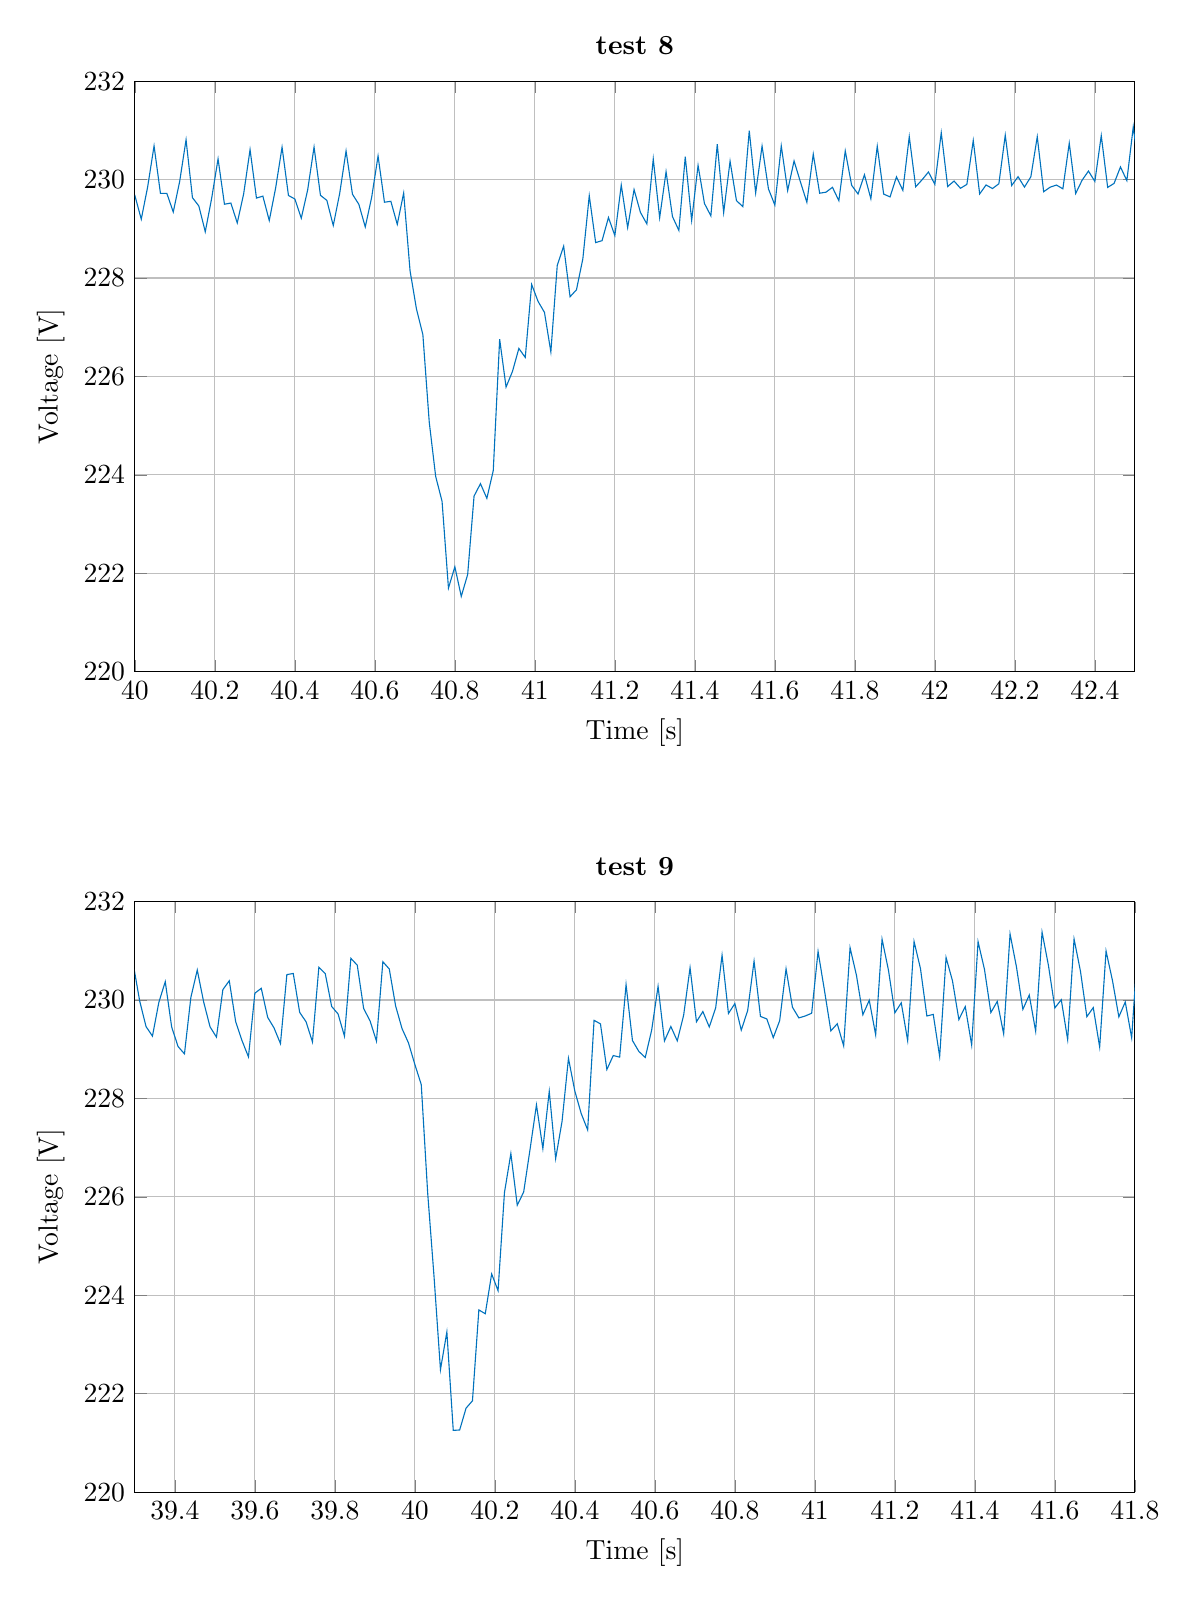
\begin{tikzpicture}

\begin{axis}[%
width=5in,
height=2.953in,
at={(1.142in,5.054in)},
scale only axis,
xmin=40,
xmax=42.5,
xlabel={Time [s]},
xmajorgrids,
ymin=220,
ymax=232,
ylabel={Voltage [V]},
ymajorgrids,
axis background/.style={fill=white},
title style={font=\bfseries},
title={test 8}
]
\addplot [color=mycolor1,solid,forget plot]
  table[row sep=crcr]{%
39.984	229.603470877899\\
40	229.676312165151\\
40.016	229.194592404445\\
40.032	229.851083466585\\
40.048	230.683399215717\\
40.064	229.717636105113\\
40.08	229.717555812167\\
40.096	229.339976231566\\
40.112	229.960646379741\\
40.128	230.807328790924\\
40.144	229.631249700769\\
40.16	229.462615543965\\
40.176	228.938668111253\\
40.192	229.618403762577\\
40.208	230.420002788047\\
40.224	229.498332285925\\
40.24	229.522259121853\\
40.256	229.118940303696\\
40.272	229.708381977131\\
40.288	230.607899346396\\
40.304	229.623700816022\\
40.32	229.662708842184\\
40.336	229.166611847126\\
40.352	229.830851260776\\
40.368	230.657161294545\\
40.384	229.676077579585\\
40.4	229.604519145093\\
40.416	229.214052887828\\
40.432	229.788124695872\\
40.448	230.660675877931\\
40.464	229.679216679488\\
40.48	229.576084955171\\
40.496	229.066190243604\\
40.512	229.713818042475\\
40.528	230.580372275807\\
40.544	229.701273828344\\
40.56	229.495895048248\\
40.576	229.036403827056\\
40.592	229.637823982224\\
40.608	230.478811857926\\
40.624	229.539215778015\\
40.64	229.557790416363\\
40.656	229.089090106648\\
40.672	229.725508041513\\
40.688	228.145404594434\\
40.704	227.371152330307\\
40.72	226.850369040369\\
40.736	225.067260056974\\
40.752	223.969460856129\\
40.768	223.461404083249\\
40.784	221.699266485029\\
40.8	222.131570394474\\
40.816	221.530826099908\\
40.832	221.974286665762\\
40.848	223.568702949398\\
40.864	223.819907384035\\
40.88	223.523161500473\\
40.896	224.085725173237\\
40.912	226.756008260959\\
40.928	225.783312586139\\
40.944	226.100211841222\\
40.96	226.568356565034\\
40.976	226.385444461583\\
40.992	227.867735253133\\
41.008	227.524076886023\\
41.024	227.301463433923\\
41.04	226.498090893529\\
41.056	228.259296523205\\
41.072	228.646499768057\\
41.088	227.618236175859\\
41.104	227.759826442425\\
41.12	228.391244177568\\
41.136	229.671443016876\\
41.152	228.71908324782\\
41.168	228.758127040357\\
41.184	229.227832642985\\
41.2	228.861627154676\\
41.216	229.887350830736\\
41.232	229.023929878925\\
41.248	229.795685136493\\
41.264	229.33118494774\\
41.28	229.09859024179\\
41.296	230.418491386258\\
41.312	229.223790810989\\
41.328	230.158365041501\\
41.344	229.247936698356\\
41.36	228.96640471732\\
41.376	230.46316409959\\
41.392	229.169599832963\\
41.408	230.287782796537\\
41.424	229.5132729945\\
41.44	229.262262303371\\
41.456	230.718135437436\\
41.472	229.330288803874\\
41.488	230.372353530648\\
41.504	229.57082589941\\
41.52	229.450031842589\\
41.536	230.992507802526\\
41.552	229.728135735208\\
41.568	230.680071665386\\
41.584	229.808742431885\\
41.6	229.481185974456\\
41.616	230.683176108015\\
41.632	229.776887479283\\
41.648	230.377988366188\\
41.664	229.949136633382\\
41.68	229.538143098871\\
41.696	230.515476007127\\
41.712	229.722096121419\\
41.728	229.743854409472\\
41.744	229.842070558922\\
41.76	229.569977799717\\
41.776	230.580894916615\\
41.792	229.882361673683\\
41.808	229.705823301768\\
41.824	230.096546979126\\
41.84	229.609340151519\\
41.856	230.676442997835\\
41.872	229.704401024046\\
41.888	229.647048799177\\
41.904	230.053889011409\\
41.92	229.780108104251\\
41.936	230.87219186443\\
41.952	229.85321463451\\
41.968	229.994507238923\\
41.984	230.153481093022\\
42	229.902072460373\\
42.016	230.950176514592\\
42.032	229.857294790684\\
42.048	229.969607424457\\
42.064	229.822524975388\\
42.08	229.900858393728\\
42.096	230.793576168335\\
42.112	229.707585385976\\
42.128	229.889868297599\\
42.144	229.817159821739\\
42.16	229.913663481962\\
42.176	230.901801716387\\
42.192	229.878122964753\\
42.208	230.057795538475\\
42.224	229.846409929028\\
42.24	230.056527835258\\
42.256	230.868996986354\\
42.272	229.752694692572\\
42.288	229.843738763543\\
42.304	229.887960583974\\
42.32	229.811367251382\\
42.336	230.739337163475\\
42.352	229.716234091412\\
42.368	229.98479013125\\
42.384	230.172405573965\\
42.4	229.961369708567\\
42.416	230.892717029205\\
42.432	229.840822133191\\
42.448	229.920944330145\\
42.464	230.255961366124\\
42.48	229.978071735042\\
42.496	231.070184973428\\
42.512	230.083005885533\\
};
\end{axis}

\begin{axis}[%
width=5in,
height=2.953in,
at={(1.142in,0.952in)},
scale only axis,
xmin=39.3,
xmax=41.8,
xlabel={Time [s]},
xmajorgrids,
ymin=220,
ymax=232,
ylabel={Voltage [V]},
ymajorgrids,
axis background/.style={fill=white},
title style={font=\bfseries},
title={test 9}
]
\addplot [color=mycolor1,solid,forget plot]
  table[row sep=crcr]{%
39.296	230.727674727276\\
39.312	229.981202868004\\
39.328	229.457943408347\\
39.344	229.265706941956\\
39.36	229.952824002461\\
39.376	230.371241393885\\
39.392	229.451135683451\\
39.408	229.053912691045\\
39.424	228.904455485639\\
39.44	230.050832434117\\
39.456	230.607392305223\\
39.472	229.959094929757\\
39.488	229.452486363607\\
39.504	229.24500543926\\
39.52	230.208520475751\\
39.536	230.39010517338\\
39.552	229.560514056165\\
39.568	229.171333515001\\
39.584	228.84313248636\\
39.6	230.136005943727\\
39.616	230.236943642993\\
39.632	229.647734656179\\
39.648	229.429612987181\\
39.664	229.113404588829\\
39.68	230.514649678157\\
39.696	230.537903912051\\
39.712	229.747831826677\\
39.728	229.556427768241\\
39.744	229.146525644521\\
39.76	230.664163036274\\
39.776	230.534257541437\\
39.792	229.867977391768\\
39.808	229.715248657584\\
39.824	229.264563800511\\
39.84	230.844853726698\\
39.856	230.706379389396\\
39.872	229.825190440191\\
39.888	229.574582463933\\
39.904	229.163776897185\\
39.92	230.77651062658\\
39.936	230.629707450441\\
39.952	229.874903326151\\
39.968	229.416249517909\\
39.984	229.1281644127\\
40	228.688345556258\\
40.016	228.27999196345\\
40.032	226.081928469266\\
40.048	224.372488674972\\
40.064	222.488244220438\\
40.08	223.253742313141\\
40.096	221.253989669401\\
40.112	221.26248286884\\
40.128	221.705604639858\\
40.144	221.855365636593\\
40.16	223.702071910459\\
40.176	223.623774061864\\
40.192	224.433278568218\\
40.208	224.092877065539\\
40.224	226.086884836244\\
40.24	226.878634274317\\
40.256	225.829185663526\\
40.272	226.096507567223\\
40.288	226.966686140891\\
40.304	227.867436949751\\
40.32	226.97964802137\\
40.336	228.141971506431\\
40.352	226.7769395201\\
40.368	227.534187332684\\
40.384	228.813697313019\\
40.4	228.14503771849\\
40.416	227.688661053867\\
40.432	227.359233913841\\
40.448	229.585552789871\\
40.464	229.513926628282\\
40.48	228.586163372013\\
40.496	228.870867989985\\
40.512	228.83831118413\\
40.528	230.310269216242\\
40.544	229.17511573334\\
40.56	228.953637976152\\
40.576	228.831244402814\\
40.592	229.385963604811\\
40.608	230.276119774119\\
40.624	229.167196768594\\
40.64	229.459610014286\\
40.656	229.169212650093\\
40.672	229.691680941362\\
40.688	230.65442292809\\
40.704	229.556540699227\\
40.72	229.764059235822\\
40.736	229.451547462859\\
40.752	229.837073122077\\
40.768	230.908704482791\\
40.784	229.724719501226\\
40.8	229.92675603694\\
40.816	229.385956229808\\
40.832	229.78390394529\\
40.848	230.787936595628\\
40.864	229.665723761356\\
40.88	229.613062867186\\
40.896	229.234390420322\\
40.912	229.578005866144\\
40.928	230.632103632788\\
40.944	229.851415951609\\
40.96	229.634802481323\\
40.976	229.674266015328\\
40.992	229.729550177645\\
41.008	230.984447863857\\
41.024	230.193701217114\\
41.04	229.371465627647\\
41.056	229.516064480832\\
41.072	229.066558669664\\
41.088	231.061921682067\\
41.104	230.499350537393\\
41.12	229.698975439632\\
41.136	229.992595783961\\
41.152	229.292362202773\\
41.168	231.233676800333\\
41.184	230.604958165953\\
41.2	229.73942241232\\
41.216	229.940801355312\\
41.232	229.172844378739\\
41.248	231.186933479321\\
41.264	230.638211722952\\
41.28	229.67422078605\\
41.296	229.705878957886\\
41.312	228.850000383342\\
41.328	230.861874922463\\
41.344	230.39017858562\\
41.36	229.601224287484\\
41.376	229.865493389104\\
41.392	229.08208145516\\
41.408	231.182950712769\\
41.424	230.621495199074\\
41.44	229.744375403367\\
41.456	229.969372716652\\
41.472	229.308900252964\\
41.488	231.341376565234\\
41.504	230.671123915275\\
41.52	229.808541265572\\
41.536	230.098640333025\\
41.552	229.364724857439\\
41.568	231.377207373361\\
41.584	230.699089706268\\
41.6	229.837639015292\\
41.616	230.004937935723\\
41.632	229.193571502076\\
41.648	231.237378589283\\
41.664	230.584263449081\\
41.68	229.659356572836\\
41.696	229.844581265617\\
41.712	229.04320922876\\
41.728	230.993287781312\\
41.744	230.39435493446\\
41.76	229.655882659834\\
41.776	229.959054676007\\
41.792	229.231414022103\\
41.808	231.158622555522\\
};
\end{axis}
\end{tikzpicture}%
\caption{Voltage disturbance on the output of the genset occuring from step of 40 to 50 kW load.}
\label{fig:test8-9-40to50kwstepvolt}
\end{figure}

\begin{figure}[H]
\centering
% This file was created by matlab2tikz.
%
%The latest updates can be retrieved from
%  http://www.mathworks.com/matlabcentral/fileexchange/22022-matlab2tikz-matlab2tikz
%where you can also make suggestions and rate matlab2tikz.
%
\definecolor{mycolor1}{rgb}{0.00000,0.44700,0.74100}%
%
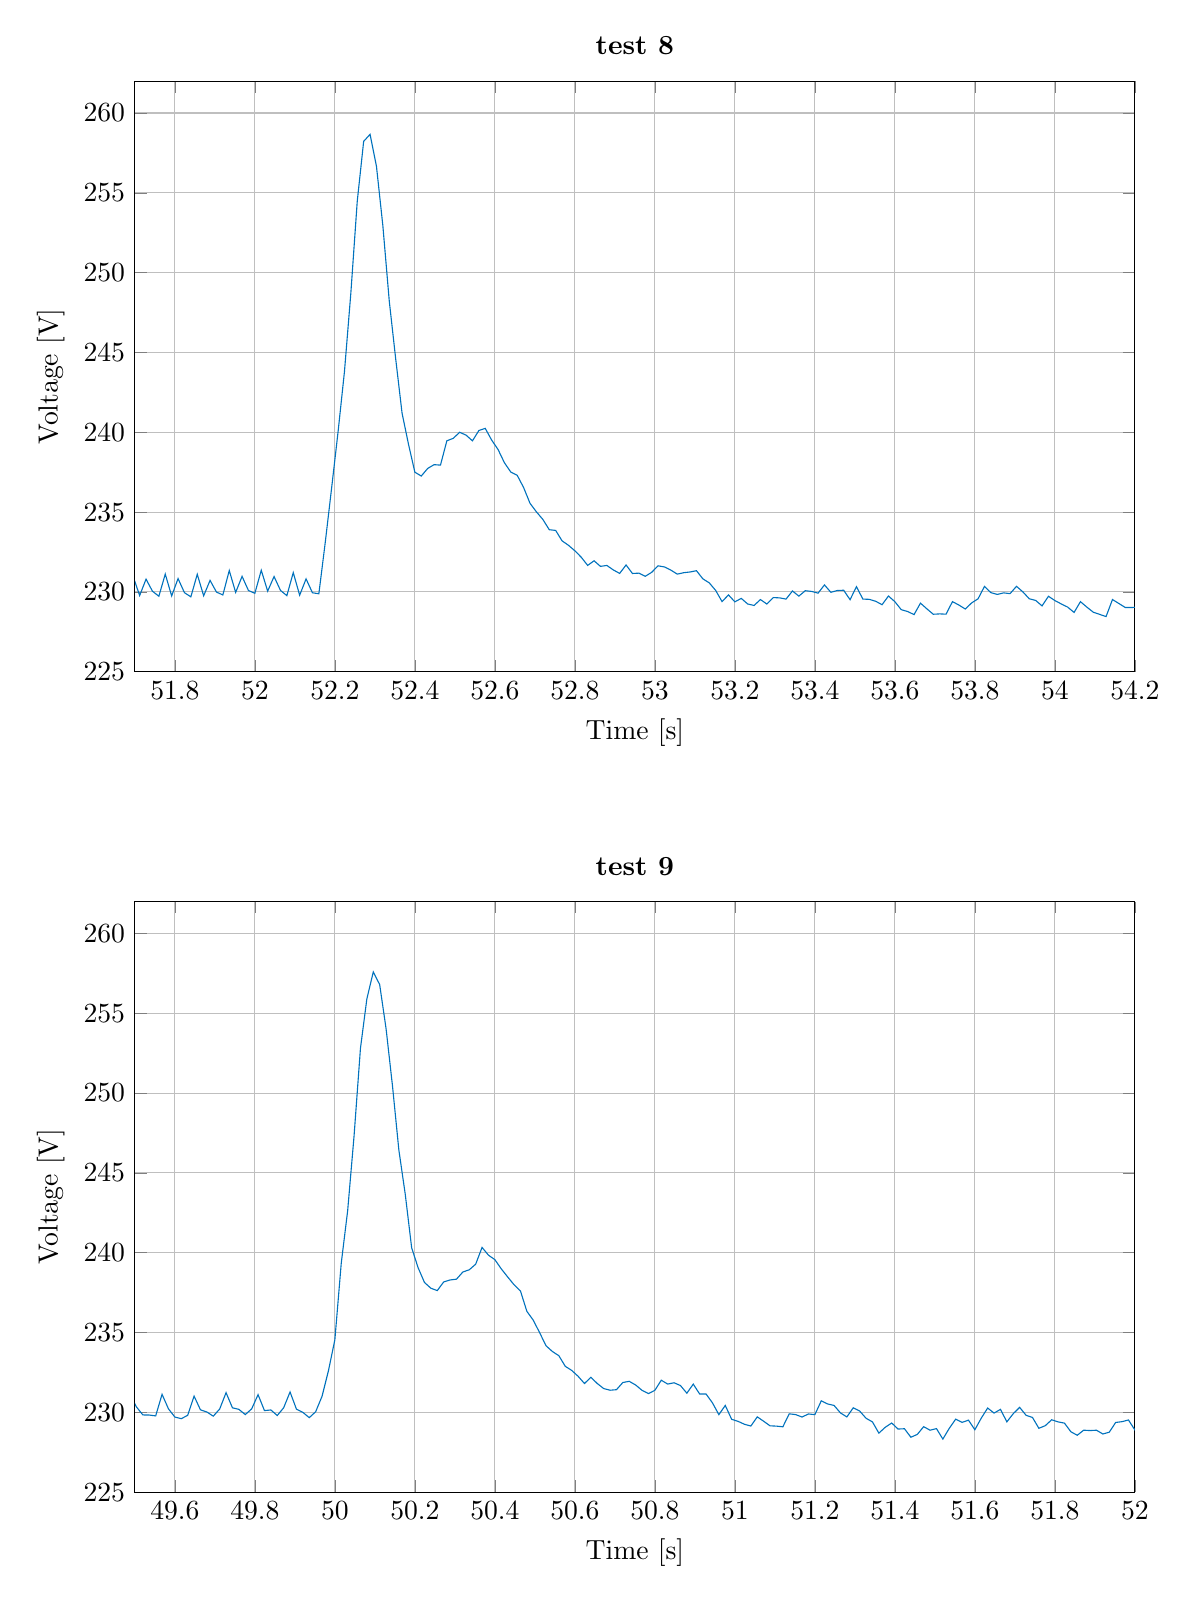
\begin{tikzpicture}

\begin{axis}[%
width=5in,
height=2.953in,
at={(1.142in,5.054in)},
scale only axis,
xmin=51.7,
xmax=54.2,
xlabel={Time [s]},
xmajorgrids,
ymin=225,
ymax=262,
ylabel={Voltage [V]},
ymajorgrids,
axis background/.style={fill=white},
title style={font=\bfseries},
title={test 8}
]
\addplot [color=mycolor1,solid,forget plot]
  table[row sep=crcr]{%
51.696	230.936732779869\\
51.712	229.771592019148\\
51.728	230.799750165026\\
51.744	230.041330364312\\
51.76	229.727924555831\\
51.776	231.115031297492\\
51.792	229.746840166115\\
51.808	230.831414157179\\
51.824	229.949793791506\\
51.84	229.690450668246\\
51.856	231.103183885909\\
51.872	229.754178033062\\
51.888	230.721292650257\\
51.904	229.988683821589\\
51.92	229.808102455342\\
51.936	231.338356801129\\
51.952	229.967843114256\\
51.968	230.973310142737\\
51.984	230.086469727026\\
52	229.911597282125\\
52.016	231.35637618068\\
52.032	230.046169368334\\
52.048	230.961997851653\\
52.064	230.095489962333\\
52.08	229.765260183157\\
52.096	231.208092129492\\
52.112	229.7922661647\\
52.128	230.814064255677\\
52.144	229.944910441015\\
52.16	229.883598057349\\
52.176	233.103467163448\\
52.192	236.530896273647\\
52.208	240.021860695048\\
52.224	243.801682128524\\
52.24	248.731677695758\\
52.256	254.478148537729\\
52.272	258.224784507178\\
52.288	258.665174278522\\
52.304	256.659488709315\\
52.32	252.939340831829\\
52.336	248.227608071287\\
52.352	244.619485865675\\
52.368	241.19758579741\\
52.384	239.259614817024\\
52.4	237.498010698501\\
52.416	237.257731659172\\
52.432	237.731298844162\\
52.448	237.970638039872\\
52.464	237.941856834171\\
52.48	239.466331220637\\
52.496	239.620885846535\\
52.512	239.999990928963\\
52.528	239.821526506901\\
52.544	239.462628297451\\
52.56	240.109557249938\\
52.576	240.242117387954\\
52.592	239.510929707029\\
52.608	238.920280619444\\
52.624	238.086298639956\\
52.64	237.503104705747\\
52.656	237.300468781156\\
52.672	236.529651571272\\
52.688	235.543776901736\\
52.704	235.010909443344\\
52.72	234.539558134396\\
52.736	233.896425074278\\
52.752	233.851329821898\\
52.768	233.198130571621\\
52.784	232.92053290154\\
52.8	232.575370060116\\
52.816	232.170346665768\\
52.832	231.65951379833\\
52.848	231.948154675142\\
52.864	231.599760681354\\
52.88	231.656180393033\\
52.896	231.378613068686\\
52.912	231.157809510803\\
52.928	231.68595414062\\
52.944	231.153990520613\\
52.96	231.173382603832\\
52.976	230.977492430834\\
52.992	231.224912752624\\
53.008	231.633311214377\\
53.024	231.561547700245\\
53.04	231.364258555558\\
53.056	231.113114876892\\
53.072	231.2020942548\\
53.088	231.247928779617\\
53.104	231.326413913924\\
53.12	230.817680460893\\
53.136	230.564485048448\\
53.152	230.093414316384\\
53.168	229.390855752201\\
53.184	229.811000915172\\
53.2	229.376405503898\\
53.216	229.593306743617\\
53.232	229.243149798697\\
53.248	229.149792698853\\
53.264	229.519048274897\\
53.28	229.238618465897\\
53.296	229.644715453057\\
53.312	229.625147435141\\
53.328	229.548649779037\\
53.344	230.057688398832\\
53.36	229.735864211732\\
53.376	230.073039975016\\
53.392	230.030205687935\\
53.408	229.921347451039\\
53.424	230.436152749929\\
53.44	229.973507771887\\
53.456	230.086564490068\\
53.472	230.10370520467\\
53.488	229.511759127843\\
53.504	230.326505452506\\
53.52	229.549444943934\\
53.536	229.533276804256\\
53.552	229.412062165267\\
53.568	229.198188299745\\
53.584	229.741706802242\\
53.6	229.388141880478\\
53.616	228.88619994636\\
53.632	228.769188538355\\
53.648	228.577489685904\\
53.664	229.296312186225\\
53.68	228.938590382745\\
53.696	228.599468196721\\
53.712	228.621323564953\\
53.728	228.604941351347\\
53.744	229.389469411606\\
53.76	229.177272157488\\
53.776	228.927849130193\\
53.792	229.310455615037\\
53.808	229.566693866833\\
53.824	230.341240869525\\
53.84	229.954899319145\\
53.856	229.841166078019\\
53.872	229.938612966906\\
53.888	229.891242645201\\
53.904	230.348673237045\\
53.92	230.002715509057\\
53.936	229.569190083158\\
53.952	229.464669897167\\
53.968	229.122214228278\\
53.984	229.726229138092\\
54	229.458109848735\\
54.016	229.246034149286\\
54.032	229.04848835729\\
54.048	228.712901721797\\
54.064	229.387334477315\\
54.08	229.046145108351\\
54.096	228.728657800801\\
54.112	228.59098098919\\
54.128	228.453625284899\\
54.144	229.521766260385\\
54.16	229.273952551101\\
54.176	229.022459324464\\
54.192	229.019017057087\\
54.208	229.054685690744\\
};
\end{axis}

\begin{axis}[%
width=5in,
height=2.953in,
at={(1.142in,0.952in)},
scale only axis,
xmin=49.5,
xmax=52,
xlabel={Time [s]},
xmajorgrids,
ymin=225,
ymax=262,
ylabel={Voltage [V]},
ymajorgrids,
axis background/.style={fill=white},
title style={font=\bfseries},
title={test 9}
]
\addplot [color=mycolor1,solid,forget plot]
  table[row sep=crcr]{%
49.488	231.109237128952\\
49.504	230.335402033574\\
49.52	229.835022801514\\
49.536	229.828609829488\\
49.552	229.773127645266\\
49.568	231.125821009866\\
49.584	230.216290773809\\
49.6	229.702290561964\\
49.616	229.600429346489\\
49.632	229.808313659376\\
49.648	231.015157372601\\
49.664	230.155704551112\\
49.68	230.01843670837\\
49.696	229.757232179027\\
49.712	230.20326091966\\
49.728	231.229014378745\\
49.744	230.280131631129\\
49.76	230.185730696904\\
49.776	229.856217392917\\
49.792	230.212941646154\\
49.808	231.1054043136\\
49.824	230.104745152132\\
49.84	230.146786032896\\
49.856	229.797649533345\\
49.872	230.284152158071\\
49.888	231.272378010333\\
49.904	230.195003106818\\
49.92	229.994186743015\\
49.936	229.664184019925\\
49.952	230.034541030786\\
49.968	231.004727592887\\
49.984	232.608849944352\\
50	234.542371559494\\
50.016	239.344171442226\\
50.032	242.630988831072\\
50.048	247.310191396818\\
50.064	252.8064985419\\
50.08	255.89892721461\\
50.096	257.584380630543\\
50.112	256.798544553788\\
50.128	254.038529033163\\
50.144	250.466146381598\\
50.16	246.432878685962\\
50.176	243.654406905154\\
50.192	240.306935516288\\
50.208	239.06611696505\\
50.224	238.133976279832\\
50.24	237.773601754535\\
50.256	237.624646932268\\
50.272	238.165671417421\\
50.288	238.289930924149\\
50.304	238.339662964796\\
50.32	238.789008568196\\
50.336	238.92878293401\\
50.352	239.276459871103\\
50.368	240.329805615155\\
50.384	239.842440180125\\
50.4	239.563374936438\\
50.416	238.986547952747\\
50.432	238.481097948783\\
50.448	237.989302406687\\
50.464	237.599527371688\\
50.48	236.325046954431\\
50.496	235.772505061222\\
50.512	234.983580422364\\
50.528	234.166398380655\\
50.544	233.805484516584\\
50.56	233.544792562438\\
50.576	232.880372883474\\
50.592	232.626525216477\\
50.608	232.258864540254\\
50.624	231.80399841188\\
50.64	232.189772298932\\
50.656	231.805483615009\\
50.672	231.488350295455\\
50.688	231.383174339905\\
50.704	231.41654938681\\
50.72	231.866735673339\\
50.736	231.94006710884\\
50.752	231.709434112708\\
50.768	231.374492052163\\
50.784	231.172649041166\\
50.8	231.377565393569\\
50.816	232.010750710373\\
50.832	231.769129925122\\
50.848	231.849437672981\\
50.864	231.675453288543\\
50.88	231.196614582357\\
50.896	231.765866895938\\
50.912	231.145144761924\\
50.928	231.145652791359\\
50.944	230.59149741134\\
50.96	229.852527489001\\
50.976	230.429037739168\\
50.992	229.559815108241\\
51.008	229.43277253525\\
51.024	229.249882615293\\
51.04	229.138739560105\\
51.056	229.713421698643\\
51.072	229.438431317274\\
51.088	229.151796263472\\
51.104	229.13362102083\\
51.12	229.090920267695\\
51.136	229.9046016762\\
51.152	229.856070686581\\
51.168	229.702801613336\\
51.184	229.896185838471\\
51.2	229.852441008415\\
51.216	230.716376578126\\
51.232	230.522149889848\\
51.248	230.42934793112\\
51.264	229.960945365147\\
51.28	229.709781821567\\
51.296	230.282393836991\\
51.312	230.078174299614\\
51.328	229.625069639994\\
51.344	229.397321997565\\
51.36	228.695447519802\\
51.376	229.061253408045\\
51.392	229.330734168075\\
51.408	228.951130719002\\
51.424	228.969367560691\\
51.44	228.438201751168\\
51.456	228.612361785419\\
51.472	229.098785756002\\
51.488	228.877763244495\\
51.504	228.977986348081\\
51.52	228.322244918868\\
51.536	228.994442628796\\
51.552	229.56810565875\\
51.568	229.366902892308\\
51.584	229.507758655956\\
51.6	228.908140674205\\
51.616	229.632830527364\\
51.632	230.266842165893\\
51.648	229.9508868619\\
51.664	230.182432665654\\
51.68	229.401563936876\\
51.696	229.912897173159\\
51.712	230.309350476062\\
51.728	229.812241422774\\
51.744	229.679142952203\\
51.76	228.99806029594\\
51.776	229.160903754459\\
51.792	229.531456847879\\
51.808	229.400216130573\\
51.824	229.321761868886\\
51.84	228.781124855013\\
51.856	228.560687871227\\
51.872	228.878671000103\\
51.888	228.854957964966\\
51.904	228.87771121858\\
51.92	228.640737898571\\
51.936	228.753874701362\\
51.952	229.362727545287\\
51.968	229.413841872984\\
51.984	229.51891856269\\
52	228.895546463599\\
52.016	229.295659123807\\
};
\end{axis}
\end{tikzpicture}%
\caption{Voltage disturbance on the output of the genset occuring from step of 50 to 10 kW load.}
\label{fig:test8-9-50to10kwstepvolt}
\end{figure}

\subsection*{Results:}




From \figref{fig:test8-9power} the steps in load is shown and the disturbance in frequency and voltage are illustrated on \figref{fig:test8-9freq} and \figref{fig:test8-9volt}. When the step is applied it can been seen on \figref{fig:test8-9freq} and \figref{fig:test8-9volt} that the governor and AVR is able to correct the disturbance and make the system stable. 

From \figref{fig:test8-9steadyfrequency10kw} to \figref{fig:test8-9-50to10kwstepvolt} steady state and step measurements is shown these will be used to compare the test where the controller is added to see if there are any change in in either stability or response time.




\subsection*{Conclusion}
It can be conclude that the governor and AVR is able to handle the disturbance that occur when a step is applied in load.